\documentclass[
twoside, % book layout
openright, % start new chapter on the right side
titlepage,
numbers=noenddot, % "Figure 2.3", not "Figure 2.3."
cleardoublepage=empty,
fontsize=11pt,
% draft,
% bindingoffset=0pt,
headings=optiontoheadandtoc,
american]{scrbook}


%%%%%%%%%%%%%%%%%%%%%%%%%%%%%%%%%%%%%%%%%%%%%%%%%%%%%%%%%%%%%%%%%%%%%%
%% Input preamble stuff

%%%%%%%%%%%%%%%%%%%%%%%%%%%%%%%%%%%%%%%%%%%%%%%%%%%%%%%%%%%%%%%%%%%%%%
%% Packages

\usepackage{scrhack}

\usepackage[ngerman,main=american]{babel}

\usepackage{calc}

\usepackage{printlen}

\usepackage{nicefrac}
\usepackage{xfrac}
\usepackage[super]{nth} %\nth{1}, \nth{2}, \nth{3}, \nth{4}

% SI units
\usepackage{eurosym}
\usepackage[binary-units=true]{siunitx}
\sisetup{
    % quotient-mode = fraction,
    per-mode = fraction,
    fraction-function=\sfrac,
    % product-units = single,
    % output-product={\,},
    unit-color = UNITCOLOR,
    % round-mode=places,
    % round-precision=2,
    % exponent-product = \cdot,
    % output-decimal-marker = {.},
    % fraction=sfrac,
    group-separator = {\,},
    group-minimum-digits = 3,
}
% \sisetup{}
\DeclareSIUnit \var { \si{\volt}\si{\ampere}r } %volt-ampere reactive - idle
% power
\DeclareSIUnit \EUR { \text{\euro} } %euro as unit
\DeclareSIUnit\year{a}

\usepackage{xargs}       % Use more than one optional parameter in a new commands

\usepackage{complexity}

\usepackage{pifont} % for \ding{55} -> cross

% Figures
\usepackage{graphicx}
\input{insbox}
\usepackage{wrapfig}
\usepackage{cutwin}

% \usepackage[redeflists]{IEEEtrantools}

% Table
\usepackage{tabularx}
\usepackage{multirow}
\usepackage{booktabs}
\def\sharedaffiliation{%
  \end{tabular}
  \begin{tabular}{c}
}
\usepackage{colortbl}
\usepackage{pdflscape}
% \usepackage{lscape}

% Quotes
\usepackage{csquotes}

\usepackage{timetravel}
\setcounter{equation}{70}
\setCounters{chapter,equation,section,figure}%algocfproc,theorem,algocf



\makeatletter%https://tex.stackexchange.com/questions/265841/small-overleftrightarrow
    \newcommand{\overleftrightsmallarrow}{\mathpalette{\overarrowsmall@\leftrightarrowfill@}}
    \newcommand{\overrightsmallarrow}{\mathpalette{\overarrowsmall@\rightarrowfill@}}
    \newcommand{\overleftsmallarrow}{\mathpalette{\overarrowsmall@\leftarrowfill@}}
% 
    \newcommand{\overarrowsmall@}[3]{%
    \vbox{%
      \ialign{%
        ##\crcr
        #1{\smaller@style{#2}}\crcr
        \noalign{\nointerlineskip}%
        $\m@th\hfil#2#3\hfil$\crcr
      }%
    }%
    }
    \def\smaller@style#1{%
    \ifx#1\displaystyle\scriptstyle\else
      \ifx#1\textstyle\scriptstyle\else
        \scriptscriptstyle
      \fi
    \fi
    }
\makeatother

%% New environment for research question
% \DeclareFloatingEnvironment{researchquestion}[Research Question][List of
% research questions]
% \crefformat{enumi}{#2Reseacrh Questions #1#3}
% \renewenvironment{researchquestion}
%   {\begin{enumerate}}
%   {\end{enumerate}}

%%%%%%%%%%%%%%%%%%%%%%%%%%%%%%%%%%%%%%%%%%%%%%%%%%%%%%%%%%%%%%%%%%%%%%
%% Indentation

\newlength{\myparindent}
\newlength{\myparskip}
\setlength{\myparindent}{1em}
\setlength{\myparskip}{0em}

\setlength{\parindent}{\myparindent}
\setlength{\parskip}{\myparskip}
\setlength{\parskip}{0pt plus1pt minus0pt}


%%%%%%%%%%%%%%%%%%%%%%%%%%%%%%%%%%%%%%%%%%%%%%%%%%%%%%%%%%%%%%%%%%%%%%
%% Colors

% \usepackage[dvipsnames]{xcolor}
\usepackage[table,x11names,dvipsnames,table]{xcolor}
\usepackage[most]{tcolorbox}

% Thesis, KIT, and power grid colors
\usepackage{transparent}

% Thesis colors
\definecolor{thesisblue}         {rgb}{0.337, 0.592, 0.773}
\definecolor{thesisblue-dark}    {rgb}{0.212, 0.471, 0.655}
\definecolor{thesisblue-light}   {rgb}{0.490, 0.710, 0.867}
\definecolor{thesisblue-vlight}  {rgb}{0.871, 0.937, 0.988}

\definecolor{thesisred}          {rgb}{0.776, 0.357, 0.396}
\definecolor{thesisred-dark}     {rgb}{0.663, 0.235, 0.271}
\definecolor{thesisred-light}    {rgb}{0.867, 0.502, 0.533}
\definecolor{thesisred-vlight}   {rgb}{0.984, 0.871, 0.878}

\definecolor{thesisgreen}        {rgb}{0.337, 0.765, 0.235}
\definecolor{thesisgreen-dark}   {rgb}{0.267, 0.612, 0.184}
\definecolor{thesisgreen-light}  {rgb}{0.443, 0.871, 0.341}
\definecolor{thesisgreen-vlight} {rgb}{0.710, 0.984, 0.643}

\definecolor{thesisyellow}       {rgb}{0.808, 0.659, 0.263}
\definecolor{thesisyellow-dark}  {rgb}{0.667, 0.529, 0.180}
\definecolor{thesisyellow-light} {rgb}{0.898, 0.765, 0.412}
\definecolor{thesisyellow-vlight}{rgb}{0.992, 0.933, 0.776}

\definecolor{black}              {rgb}{0,0,0}
\definecolor{black70}            {rgb}{0.30,0.30,0.30}
\definecolor{black50}            {rgb}{0.50,0.50,0.50}
\definecolor{black30}            {rgb}{0.70,0.70,0.70}
\definecolor{black15}            {rgb}{0.85,0.85,0.85}
\definecolor{black7}             {rgb}{0.95,0.95,0.95}

% Set major colors
\colorlet{primarycolor-dark}      {thesisblue-dark}
\colorlet{primarycolor}           {thesisblue}
\colorlet{primarycolor-light}     {thesisblue-light}
\colorlet{primarycolor-vlight}    {thesisblue-vlight}
\colorlet{secondarycolor-dark}    {thesisred-dark}
\colorlet{secondarycolor}         {thesisred}
\colorlet{secondarycolor-light}   {thesisred-light}
\colorlet{secondarycolor-vlight}  {thesisred-vlight}

\colorlet{stroke1}                {primarycolor-dark}
\colorlet{stroke2}                {secondarycolor-dark}

% Set document colors
\colorlet{captionlabel}{black}
\colorlet{footerpagenr}{black}
\colorlet{footerchapter}{stroke1}
\colorlet{footerchaptername}{black}
\colorlet{footersection}{stroke1}
\colorlet{footersectionname}{black}
\colorlet{chapternumber}{stroke1}
\colorlet{sectiontitlenumber}{black}
\colorlet{sectiontitle}{black}

% ACM already defined colors
\definecolor[named]{ACMBlue}{cmyk}{1,0.1,0,0.1}
\definecolor[named]{ACMYellow}{cmyk}{0,0.16,1,0}
\definecolor[named]{ACMOrange}{cmyk}{0,0.42,1,0.01}
\definecolor[named]{ACMRed}{cmyk}{0,0.90,0.86,0}
\definecolor[named]{ACMLightBlue}{cmyk}{0.49,0.01,0,0}
\definecolor[named]{ACMGreen}{cmyk}{0.20,0,1,0.19}
\definecolor[named]{ACMPurple}{cmyk}{0.55,1,0,0.15}
\definecolor[named]{ACMDarkBlue}{cmyk}{1,0.58,0,0.21}

%  
% \definecolor{orange}{HTML}{FF7F00}
% \definecolor{orange}{rgb}{1,0.5,0}
% \definecolor{orange}{RGB}{255,127,0}
% \definecolor{figChar}{cmyk}{0,0.90,0.86,0}

% KIT Colors
% KIT green
\definecolor{KITgreen}{rgb}{0 0.588 0.509}
\definecolor{KITgreen70}{rgb}{0.3 0.711 0.656}
\definecolor{KITgreen50}{rgb}{0.5 0.794 0.754}
\definecolor{KITgreen30}{rgb}{0.7 0.876 0.852}
\definecolor{KITgreen15}{rgb}{0.85 0.938 0.926}
% KIT palegreen
\definecolor{KITpalegreen}{rgb}{0.509,0.745,0.235}
\definecolor{KITpalegreen70}{rgb}{0.656,0.821,0.464}
\definecolor{KITpalegreen50}{rgb}{0.754,0.872,0.617}
\definecolor{KITpalegreen30}{rgb}{0.852,0.923,0.77}
\definecolor{KITpalegreen15}{rgb}{0.926,0.961,0.885}
% KIT yellow
\definecolor{KITyellow}{rgb}{0.98,0.901,0.078}
\definecolor{KITyellow70}{rgb}{0.986,0.931,0.354}
\definecolor{KITyellow50}{rgb}{0.99,0.95,0.539}
\definecolor{KITyellow30}{rgb}{0.994,0.97,0.723}
\definecolor{KITyellow15}{rgb}{0.997,0.985,0.861}
% KIT orange
\definecolor{KITorange}{rgb}{0.862,0.627,0.117}
\definecolor{KITorange70}{rgb}{0.903,0.739,0.382}
\definecolor{KITorange50}{rgb}{0.931,0.813,0.558}
\definecolor{KITorange30}{rgb}{0.958,0.888,0.735}
\definecolor{KITorange15}{rgb}{0.979,0.944,0.867}
% KIT brown
\definecolor{KITbrown}{rgb}{0.627,0.509,0.196}
\definecolor{KITbrown70}{rgb}{0.739,0.656,0.437}
\definecolor{KITbrown50}{rgb}{0.813,0.754,0.598}
\definecolor{KITbrown30}{rgb}{0.888,0.852,0.758}
\definecolor{KITbrown15}{rgb}{0.944,0.926,0.879}
% KIT red
\definecolor{KITred}{rgb}{0.627,0.117,0.156}
\definecolor{KITred70}{rgb}{0.739,0.382,0.409}
\definecolor{KITred50}{rgb}{0.813,0.558,0.578}
\definecolor{KITred30}{rgb}{0.888,0.735,0.747}
\definecolor{KITred15}{rgb}{0.944,0.867,0.873}
% KIT lilac
\definecolor{KITlilac}{rgb}{0.627,0,0.47}
\definecolor{KITlilac70}{rgb}{0.739,0.3,0.629}
\definecolor{KITlilac50}{rgb}{0.813,0.5,0.735}
\definecolor{KITlilac30}{rgb}{0.888,0.7,0.841}
\definecolor{KITlilac15}{rgb}{0.944,0.85,0.92}
% KIT blue
\definecolor{KITblue}{rgb}{0.274,0.392,0.666}
\definecolor{KITblue70}{rgb}{0.492,0.574,0.766}
\definecolor{KITblue50}{rgb}{0.637,0.696,0.833}
\definecolor{KITblue30}{rgb}{0.782,0.817,0.9}
\definecolor{KITblue15}{rgb}{0.891,0.908,0.95}
% KIT seablue
\definecolor{KITseablue}{rgb}{0.196,0.313,0.549}
\definecolor{KITseablue70}{rgb}{0.437,0.519,0.684}
\definecolor{KITseablue50}{rgb}{0.598,0.656,0.774}
\definecolor{KITseablue30}{rgb}{0.758,0.794,0.864}
\definecolor{KITseablue15}{rgb}{0.879,0.897,0.932}
% KIT cyanblue
\definecolor{KITcyanblue}{rgb}{0.313,0.666,0.901}
\definecolor{KITcyanblue70}{rgb}{0.519,0.766,0.931}
\definecolor{KITcyanblue50}{rgb}{0.656,0.833,0.95}
\definecolor{KITcyanblue30}{rgb}{0.794,0.9,0.97}
\definecolor{KITcyanblue15}{rgb}{0.897,0.95,0.985}
% KIT black
\definecolor{KITblack}{rgb}{0,0,0}
\definecolor{KITblack70}{rgb}{0.3,0.3,0.3}
\definecolor{KITblack50}{rgb}{0.5,0.5,0.5}
\definecolor{KITblack30}{rgb}{0.7,0.7,0.7}
\definecolor{KITblack15}{rgb}{0.85,0.85,0.85}

% Power Grid specific colors
\definecolor{FEASIBLE}{rgb}{0.739,0.3,0.629}
\definecolor{PHYSICAL}{rgb}{0.437,0.519,0.684}
\definecolor{KVL}{rgb}{0.437,0.519,0.684}
\definecolor{KCL}{rgb}{0.739,0.3,0.629}
% Problems
\definecolor{MTSF}{rgb}{0.509,0.745,0.235}
\definecolor{MPF}{rgb}{0.437,0.519,0.684}
\definecolor{MF}{rgb}{0.739,0.3,0.629}
\definecolor{OTS}{rgb}{0,0,0}
\definecolor{ROP}{rgb}{0,0,0}
\definecolor{ROP}{rgb}{0,0,0}
\definecolor{MFF}{rgb}{0,0,0}
\definecolor{OPF}{rgb}{0,0,0}
% 
\definecolor{HELMHOLTZblue}{rgb}{0.043,0.362,0.618}
\definecolor{HELMHOLTZgreen}{rgb}{0.549,0.7,0.19}
\definecolor{CHANGES}{rgb}{0.997,0.985,0.861}
% Elements
\definecolor{GENERATOR}{rgb}{0.437,0.519,0.684}
\definecolor{CONSUMER}{rgb}{0.739,0.3,0.629}
\definecolor{SUSCEPTANCE}{rgb}{0.862,0.627,0.117}
\definecolor{SWITCHE}{rgb}{0,0.588,0.509}
\definecolor{THETA}{rgb}{0.313,0.666,0.901}
\definecolor{CAPACITY}{rgb}{0.5,0.5,0.5}
\definecolor{DTP}{rgb}{0.627,0.117,0.156}

\colorlet{Table-Line-Marker}  {KITyellow15}
\colorlet{DUALGRAPH}          {THETA}
\colorlet{PRIMALGRAPH}        {KITblack50}
\colorlet{KVLCONFLICT}        {KITred70}
\colorlet{SUBSTATION}         {KITbrown70}
\colorlet{VOLTAGE}            {KITblue70}
\colorlet{CURRENT}            {KITred70}
\colorlet{REALPOWER}          {KITcyanblue70}
\colorlet{REACTIVEPOWER}      {KITcyanblue30}
\colorlet{COMPLEXPOWER}       {KITgreen70}
\colorlet{POWERANGLE}         {KITpalegreen70}
\colorlet{TIMESTAMP}          {KITblack70}
\colorlet{UNITCOLOR}          {KITblack70}
\colorlet{ColorTableRule}     {KITblack70}
\colorlet{ColorKclConflictMarker}       {KITred70}
\colorlet{ColorSusceptanceScalingMarker}{SUSCEPTANCE}
\colorlet{ColorFACTSedge}     {KITred70}

% Wind farm cabling
\colorlet{ColorTransmissionCable}{KITseablue}
\colorlet{ColorSubstation}       {KITbrown}
\colorlet{ColorCollectionPoint}  {ColorSubstation}
\colorlet{ColorTransportCableSmall}     {KITblack50}
\colorlet{ColorTransportCableMedium}    {KITblack70}
\colorlet{ColorTransportCableLarge}     {KITblack}
\colorlet{ColorCircuitProblem}          {KITgreen}
\colorlet{ColorSubstationProblem}       {KITorange}
\colorlet{ColorFullWindFarm}            {KITred}



%%%%%%%%%%%%%%%%%%%%%%%%%%%%%%%%%%%%%%%%%%%%%%%%%%%%%%%%%%%%%%%%%%%%%%
%% Link
\newcommandx{\screen}[1]{\textcolor{black}{#1}}%
\newcommandx{\screentextcolor}[2]{\textcolor{#1}{#2}}%
\colorlet{HiLi}{KITorange15}

%%%%%%%%%%%%%%%%%%%%%%%%%%%%%%%%%%%%%%%%%%%%%%%%%%%%%%%%%%%%%%%%%%%%%%
%% Highlight text background

\usepackage{soul}
\DeclareRobustCommand{\hlhili}[1]{{\sethlcolor{HiLi}\hl{#1}}}
\DeclareRobustCommand{\myhl}[2]{{\sethlcolor{#1}\hl{#2}}}


%%%%%%%%%%%%%%%%%%%%%%%%%%%%%%%%%%%%%%%%%%%%%%%%%%%%%%%%%%%%%%%%%%%%%%
%% ...

\newlength{\tmpa}
\newlength{\tmpb}
\newlength{\tmpc}


%%%%%%%%%%%%%%%%%%%%%%%%%%%%%%%%%%%%%%%%%%%%%%%%%%%%%%%%%%%%%%%%%%%%%%
%% Size and position of the text body

\newlength{\mybodywidth}
\newlength{\mybodyheight}
\newlength{\myoutermargin}
\newlength{\mytopmargin}
\setlength{\mybodywidth}{132.5mm}
\setlength{\mybodyheight}{195mm}
\setlength{\myoutermargin}{51.8mm}%+5mm}
\setlength{\mytopmargin}{38mm}

\newlength{\myinnermargin}
\newlength{\mybottommargin}
\setlength{\myinnermargin}{\paperwidth-\mybodywidth-\myoutermargin}
\setlength{\mybottommargin}{\paperheight-\mybodyheight-\mytopmargin}


%%%%%%%%%%%%%%%%%%%%%%%%%%%%%%%%%%%%%%%%%%%%%%%%%%%%%%%%%%%%%%%%%%%%%%
%% Position of the cut marks

\newlength{\cutmarktop}
\newlength{\cutmarkbottom}
\newlength{\cutmarkinner}
\newlength{\cutmarkouter}

\setlength{\cutmarktop}{7mm}
\setlength{\cutmarkbottom}{7mm}
\setlength{\cutmarkinner}{0mm}
\setlength{\cutmarkouter}{7mm}


%%%%%%%%%%%%%%%%%%%%%%%%%%%%%%%%%%%%%%%%%%%%%%%%%%%%%%%%%%%%%%%%%%%%%%
%% Position of the head and foot

\newcommand{\goldenratio}{1.618}

\newlength{\myheadsep} % distance from header to body
\setlength{\myheadsep}{(\mytopmargin-\cutmarktop) -
  (\mytopmargin-\cutmarktop) / \real{\goldenratio} - 1ex}

\newlength{\myfootskip} % distance from body to footer
\setlength{\myfootskip}{(\mybottommargin-\cutmarkbottom) /
  \real{\goldenratio} - 1ex}


%%%%%%%%%%%%%%%%%%%%%%%%%%%%%%%%%%%%%%%%%%%%%%%%%%%%%%%%%%%%%%%%%%%%%%
%% Margin position and width

\newlength{\mymargininnersep} % distance between margin and body
\newlength{\mymarginoutersep} % distance between margin and paper edge
\newlength{\mymarginwidth} % width of the margin
\setlength{\mymargininnersep}{7mm}
\setlength{\mymarginoutersep}{12mm}
\setlength{\mymarginwidth}{\myoutermargin - \mymargininnersep -
  \mymarginoutersep - \cutmarkouter}


%%%%%%%%%%%%%%%%%%%%%%%%%%%%%%%%%%%%%%%%%%%%%%%%%%%%%%%%%%%%%%%%%%%%%%
%% Applying the geometry

\usepackage[
paper=a4paper,
width=\mybodywidth,
height=\mybodyheight,
outer=\myoutermargin,
top=\mytopmargin,
headsep=\myheadsep,
footskip=\myfootskip,
marginparsep=\mymargininnersep,
marginparwidth=\mymarginwidth
% showframe
]{geometry}

%%%%%%%%%%%%%%%%%%%%%%%%%%%%%%%%%%%%%%%%%%%%%%%%%%%%%%%%%%%%%%%%%%%%%%
%% Comments and TODOs

% for new line use "\newline"
\usepackage[colorinlistoftodos,prependcaption,textsize=tiny]{todonotes}
% 
\newcommandx{\franzi}[2][1=]{\todo
[linecolor=red,backgroundcolor=red!25,bordercolor=red,#1]{{\textbf{
\underline{Franzi:}}}\newline#2}\xspace}

%%%%%%%%%%%%%%%%%%%%%%%%%%%%%%%%%%%%%%%%%%%%%%%%%%%%%%%%%%%%%%%%%%%%%%
%% Printing crop marks

\usepackage{tikz}
\setlength{\tmpa}{1mm}
\newcommand{\cropmarkeven}{%
  \begin{tikzpicture}[overlay,remember picture]%
    \node [inner sep=0,outer sep=0, anchor=north west] at (current
    page.north west) {%
      \begin{tikzpicture}[overlay,remember picture]%
        \draw (\cutmarkouter,0mm) -- (\cutmarkouter,-\cutmarktop+\tmpa);%
        \draw (0mm,-\cutmarktop) -- (\cutmarkouter-\tmpa,-\cutmarktop);%
      \end{tikzpicture}%
    };%
    \node [inner sep=0,outer sep=0, anchor=north east] at (current
    page.north east) {%
      \begin{tikzpicture}[overlay,remember picture]%
        \draw (0mm,-\cutmarktop) -- (-\cutmarkouter+\tmpa,-\cutmarktop);%
      \end{tikzpicture}%
    };%
    \node [inner sep=0,outer sep=0, anchor=south west] at (current
    page.south west) {%
      \begin{tikzpicture}[overlay,remember picture]%
        \draw (\cutmarkouter,0mm) -- (\cutmarkouter,\cutmarktop-\tmpa);%
        \draw (0mm,\cutmarktop) -- (\cutmarkouter-\tmpa,\cutmarktop);%
      \end{tikzpicture}%
    };%
    \node [inner sep=0,outer sep=0, anchor=south east] at (current
    page.south east) {%
      \begin{tikzpicture}[overlay,remember picture]%
        \draw (0mm,\cutmarktop) -- (-\cutmarkouter+\tmpa,\cutmarktop);%
      \end{tikzpicture}%
    };%
  \end{tikzpicture}
}
\newcommand{\cropmarkodd}{%
  \begin{tikzpicture}[overlay,remember picture]%
    \node [inner sep=0,outer sep=0, anchor=north west] at (current
    page.north west) {%
      \begin{tikzpicture}[overlay,remember picture]%
        \draw (0mm,-\cutmarktop) -- (\cutmarkouter-\tmpa,-\cutmarktop);%
      \end{tikzpicture}%
    };%
    \node [inner sep=0,outer sep=0, anchor=north east] at (current
    page.north east) {%
      \begin{tikzpicture}[overlay,remember picture]%
        \draw (-\cutmarkouter,0mm) -- (-\cutmarkouter,-\cutmarktop+\tmpa);%
        \draw (0mm,-\cutmarktop) -- (-\cutmarkouter+\tmpa,-\cutmarktop);%
      \end{tikzpicture}%
    };%
    \node [inner sep=0,outer sep=0, anchor=south west] at (current
    page.south west) {%
      \begin{tikzpicture}[overlay,remember picture]%
        \draw (0mm,\cutmarktop) -- (\cutmarkouter-\tmpa,\cutmarktop);%
      \end{tikzpicture}%
    };%
    \node [inner sep=0,outer sep=0, anchor=south east] at (current
    page.south east) {%
      \begin{tikzpicture}[overlay,remember picture]%
        \draw (-\cutmarkouter,0mm) -- (-\cutmarkouter,\cutmarktop-\tmpa);%
        \draw (0mm,\cutmarktop) -- (-\cutmarkouter+\tmpa,\cutmarktop);%
      \end{tikzpicture}%
    };%
  \end{tikzpicture}
}

\usepackage{everypage}
\usepackage[strict]{changepage}

\newcommand{\showcropmarks}{%
  \AddEverypageHook{%
    \checkoddpage%
    \ifoddpage%
    \cropmarkodd%
    \else%
    % \cropmarkeven%
    \fi%
  }}


%%%%%%%%%%%%%%%%%%%%%%%%%%%%%%%%%%%%%%%%%%%%%%%%%%%%%%%%%%%%%%%%%%%%%%
%% Header and footer format

\usepackage{fancyhdr}
\pagestyle{fancy} 

\fancypagestyle{plain}{%
  \fancyhf{} % clear header and footer

  % no header/footer line
  \renewcommand{\headrulewidth}{0pt}
  \renewcommand{\footrulewidth}{0pt}

  % set distances
  \fancyheadoffset[EL]{\myoutermargin}
  \fancyheadoffset[OR]{\myoutermargin}
  \fancyfootoffset[EL]{\myoutermargin}
  \fancyfootoffset[OR]{\myoutermargin}

  % page numbers
  \fancyfoot[EL]{%
    {\color{stroke1}\rule{\myoutermargin-\mymargininnersep}{0.5mm}}\\
    \begin{minipage}[b]{\myoutermargin-\mymargininnersep}%
      \raggedleft\color{footerpagenr}\textbf{\thepage}%
    \end{minipage}%
  }
  \fancyfoot[OR]{%
    {\color{stroke1}\rule{\myoutermargin-\mymargininnersep}{0.5mm}}\\
    \begin{minipage}[b]{\myoutermargin-\mymargininnersep}%
      \raggedright\color{footerpagenr}\textbf{\thepage}%
    \end{minipage}%
  }
}

\fancypagestyle{content}{%
  % use default page numbering
  \pagestyle{plain}

  % define header
  \renewcommand{\chaptermark}[1]{%
    \markboth{%
      \small\textsf{\color{footerchaptername}##1}%
    }{}%
  }
  \renewcommand{\sectionmark}[1]{%
    \markright{%
      \small\textsf{\color{footersectionname}##1}%
    }%
  } 
  \fancyhead[EL]{%
    \begin{minipage}[b]{\myoutermargin-\mymargininnersep}%
      \small%
      \raggedleft\textsf{\textbf{\color{footerchapter}\chaptername\ \thechapter}}
    \end{minipage}%
    \hspace{\mymargininnersep}\leftmark%
  }
  \fancyhead[OR]{%
    \rightmark\hspace{\mymargininnersep}%
    \begin{minipage}[b]{\myoutermargin-\mymargininnersep}%
      \small%
      \raggedright\textsf{\textbf{\color{footersection}Section\ \thesection}}
    \end{minipage}%
  }
}


%%%%%%%%%%%%%%%%%%%%%%%%%%%%%%%%%%%%%%%%%%%%%%%%%%%%%%%%%%%%%%%%%%%%%%
%% Caption format

\usepackage{caption}
\captionsetup{
  font=small,
  labelfont={bf,sf,color=captionlabel},
  format=plain,
  singlelinecheck=off
  %tableposition=top
}

\usepackage{floatrow}
\floatsetup[table]{capposition=top}
% \usepackage{colortbl}
% \usepackage[table]{xcolor}
% \usepackage{multirow}


%%%%%%%%%%%%%%%%%%%%%%%%%%%%%%%%%%%%%%%%%%%%%%%%%%%%%%%%%%%%%%%%%%%%%%
%% part format
% \RequirePackage{silence}
% \WarningFilter{scrreprt}{Usage of package `titlesec'}
% \WarningFilter{scrreprt}{Activating an ugly workaround}

\usepackage[noindentafter,explicit]{titlesec}

\assignpagestyle{\part}{empty}
\titleformat{\part}
[display]
{\Huge\sffamily}%
{}%
{-2\baselineskip}%
{%
  \setlength{\tmpa}{0.618\paperwidth}%
  \setlength{\tmpb}{0.382\paperheight}%
  \begin{tikzpicture}[overlay,remember picture]%
    \node [inner sep=0,outer sep=0, anchor=north] at (current
    page.north west) {%
      \begin{tikzpicture}[overlay,remember picture]%
        \draw[color=stroke1, line width=0.7mm] (\tmpa,0) -- (\tmpa,-\tmpb);%
      \end{tikzpicture}%
    };%
    \node (align) [align=right, below=\tmpb-2ex, inner sep=0, outer
    sep=0, anchor=north west] at (current page.north west){%
      \hspace{\tmpa}\hspace{0.5em}\partname\ \thepart\\[1ex]%
      \color{stroke1}#1%
    };%
  \end{tikzpicture}%
}%
[]


%%%%%%%%%%%%%%%%%%%%%%%%%%%%%%%%%%%%%%%%%%%%%%%%%%%%%%%%%%%%%%%%%%%%%%
%% Chapter format
% 
\let\oldchapter\chapter
\newcommand\Chapter[3]{%
% \renewcommand\chapter[3]{%
  \def\tempSubtitle{#2}
  \def\tempFooter{#3}
  % 
  \ifx\tempSubtitle\empty
    \def\tempTocEntry{#1}
    \def\tempHeadEntry{#1}
    \ifx\tempFooter\empty
      \def\tempHeader{\sffamily\fontsize{19.5}{19.5}\selectfont#1}
    \else
      \def\tempHeader{\sffamily\fontsize{19.5}{19.5}\selectfont#1#3}
    \fi
  \else
    \def\tempTocEntry{#1\hfil\hbox{}\protect\linebreak{\normalfont\itshape#2}}%
    % \def\tempTocEntry{#1\protect\linebreak{\normalfont\itshape#2}}%
    \def\tempHeadEntry{#2}
    \ifx\tempFooter\empty
      \def\tempHeader{\sffamily\fontsize{19.5}{19.5}\selectfont#1\\[0.0ex]\Large\itshape#2}
    \else
      \def\tempHeader{\sffamily\fontsize{19.5}{19.5}\selectfont#1#3\\[0.0ex]\Large\itshape#2}
    \fi
  \fi
  % 
  \oldchapter[%
    tocentry={\tempTocEntry},
    head={\tempHeadEntry}
  ]%
  {
    \ifx\tempSubtitle\empty
      \sffamily\fontsize{19.5}{19.5}\selectfont#1\hspace{-2mm}#3
    \else
      \sffamily\fontsize{19.5}{19.5}\selectfont#1\hspace{-2mm}#3
      \\[0.0ex]\Large\itshape#2
    \fi
  }%
}

\usepackage{xpatch}
\makeatletter
\providecommand*\@chaptersubtitle{}
\FamilyStringKey[.section]{KOMAarg}{chaptersubtitle}{\@chaptersubtitle}
\xpretocmd{\chapter}{\xdef\@chaptersubtitle{}}{}{\PatchFailed}
\xapptocmd\chapterlinesformat{%
  \ifstr{\@chaptersubtitle}{}{}
    {%
      \parbox[t]{\linewidth}
        {\raggedchaptersubtitle\usekomafont{chaptersubtitle}\@chaptersubtitle}%
      \par\nobreak
    }%
  }
  {}{\PatchFailed}
\xapptocmd\chapterlineswithprefixformat{%
  \ifstr{\@chaptersubtitle}{}{}
    {%
      \parbox[t]{\linewidth}
        {\raggedchaptersubtitle\usekomafont{chaptersubtitle}\@chaptersubtitle}%
      \par\nobreak
    }%
  }
  {}{\PatchFailed}
\makeatother
\newcommand\raggedchaptersubtitle{\raggedchapter}
\newkomafont{chaptersubtitle}{\normalsize}



% \assignpagestyle{\chapter}{plain}
\titlespacing{\chapter}{0mm}{0mm}{0mm}
\titleformat{\chapter}[display]%
{\sffamily\color{stroke1}\huge}% format
{}% label
{0pt}% sep
{%
  \begin{tikzpicture}[overlay,remember picture]%
    \node [right=\myinnermargin,below=\mytopmargin, inner sep=0, outer
    sep=0, anchor=north west] (numbernode) at (current page.north west){%
      \hspace{\myinnermargin}%
      \sffamily\fontsize{60}{60}\selectfont%
      \color{chapternumber}%
      \raggedchaptersubtitle%
      \thechapter%
    };%
    \node [inner sep=0,outer sep=0, anchor=north west] at (numbernode.south west) {%
      \begin{tikzpicture}[overlay,remember picture]%
        \draw[color=stroke1, line width=0.7mm] (\myinnermargin,-1ex) -- (\paperwidth,-1ex);%
      \end{tikzpicture}%
    };%
    \node (align) [align=right, right=\myinnermargin+\mybodywidth, inner sep=0, outer sep=0,
    anchor=east] at (numbernode.west) {%
      #1%
    };%
  \end{tikzpicture}%
}% before-code
[\bigskip]% after-code


\titleformat{name=\chapter,numberless}
[display]%
{\sffamily\color{stroke1}\huge}% format
{}% label
{0pt}% sep
{%
  \begin{tikzpicture}[overlay,remember picture]%
    \node [right=\myinnermargin,below=\mytopmargin, inner sep=0, outer
    sep=0, anchor=north west] (numbernode) at (current page.north west){%
      \hspace{\myinnermargin}%
      \sffamily\fontsize{60}{60}\selectfont%
      \color{white}%
      \thechapter%
    };%
    \node [inner sep=0,outer sep=0, anchor=north west] at (numbernode.south west) {%
      \begin{tikzpicture}[overlay,remember picture]%
        \draw[color=stroke1, line width=0.7mm] (\myinnermargin,-1ex) -- (\paperwidth,-1ex);%
      \end{tikzpicture}%
    };%
    \node (align) [align=left, right=\myinnermargin, inner sep=0, outer sep=0,
    anchor=south west] at (numbernode.south west) {%
      #1%
    };%
  \end{tikzpicture}%
}% before-code
[\bigskip]% after-code


%%%%%%%%%%%%%%%%%%%%%%%%%%%%%%%%%%%%%%%%%%%%%%%%%%%%%%%%%%%%%%%%%%%%%%
%% Section format

% \titleformat{\section}%
% [block]%
% {\Large\bfseries\sffamily}%
% {\color{sectiontitlenumber}\thesection\hspace{0.5em}}%
% {0pt}%
% {\color{sectiontitle}\raggedright}%
% []


%%%%%%%%%%%%%%%%%%%%%%%%%%%%%%%%%%%%%%%%%%%%%%%%%%%%%%%%%%%%%%%%%%%%%%
%% Subsection format

% \titleformat{\subsection}%
% [block]%
% {\large\bfseries\sffamily}%
% {\color{sectiontitlenumber}\thesubsection\hspace{0.5em}}%
% {0pt}%
% {\color{sectiontitle}\raggedright}%
% []


%%%%%%%%%%%%%%%%%%%%%%%%%%%%%%%%%%%%%%%%%%%%%%%%%%%%%%%%%%%%%%%%%%%%%%
%% Paragraph format

\titleformat{\paragraph}%
[runin]%
{\bfseries\sffamily}%
{}%
{0pt}%
{#1.}%
[]


%%%%%%%%%%%%%%%%%%%%%%%%%%%%%%%%%%%%%%%%%%%%%%%%%%%%%%%%%%%%%%%%%%%%%%
%% Biblatex and CV packages

\usepackage[utf8]{inputenc}

\usepackage{currvita}
\usepackage{csquotes}
\usepackage[
style=alphabetic,
% style=trad-alpha,
%style=numeric,
autocite=plain,
maxnames=100,
backend=biber,
natbib=true,
defernumbers,
safeinputenc,
backref=true,
backrefstyle=none,
sortcites,
maxcitenames=2,
% abbreviate=true 
% citetracker=true,
% sortcites=true, 
% sorting=ynt, 
% pagetracker=true,
% backref=true,
% minnames=1,
% maxbibnames=10,
% minbibnames=7,
% uniquelist=true,
% uniquename=allfull,
]{biblatex}
% \autocite, \textcite,\parencite
\patchcmd{\bibsetup}{\interlinepenalty=5000}{\interlinepenalty=10000}{}{}

% Set up back references.
\DefineBibliographyStrings{english}{%
  backrefpage = {cited on page}, % originally "cited on page"
  backrefpages = {cited on pages}, % originally "cited on pages"
}

\DeclareFieldFormat{pagerefformat}{#1}
% \DeclareFieldFormat{pagerefformat}{\small\color{stroke1}\mkbibemph{{#1}}}

\renewbibmacro*{pageref}{%
  \addperiod%
  \iflistundef{pageref}%
    {}%
    {\newline\footnotesize\printtext[pagerefformat]{%
       \ifnumgreater{\value{pageref}}{1}%
         {\bibstring{backrefpages}\ppspace}%
     {\bibstring{backrefpage}\ppspace}%
       \printlist[pageref][-\value{listtotal}]{pageref}\addperiod}}}

% Set up bibliography layout.
\DeclareNumChars*{:}
\renewcommand{\intitlepunct}{\addspace}
\renewcommand{\multicitedelim}{\addcomma\space}

\renewbibmacro{in:}{%
  \ifentrytype{article}{}{\printtext{\bibstring{in}\intitlepunct}}}

\renewbibmacro*{volume+number+eid}{
  \printfield{volume}
  \iffieldundef{number}{}{\addcolon}%
  \printfield{number}
  \setunit*{\addcomma\space}
  \printfield{eid}
}

\renewbibmacro*{editor+others}{%
  \ifboolexpr{
    test \ifuseeditor
    and
    not test {\ifnameundef{editor}}
  }
    {\printnames{editor}%
     \setunit{\space}%
     \usebibmacro{editor+othersstrg}%
     \clearname{editor}}
    {}}

\addbibresource{bibliography/article.bib}
\addbibresource{bibliography/book.bib}
\addbibresource{bibliography/thesis.bib}
\addbibresource{bibliography/internet.bib}
% \addbibresource{bibliography/list-of-publications.bib}

% \AtEveryCitekey{\ifciteseen{}{\defcounter{maxnames}{99}}}

\DeclareFieldFormat[article]{title}{\textbf{\color{stroke1}#1}}
\DeclareFieldFormat[inproceedings]{title}{\textbf{\color{stroke1}#1}}
\DeclareFieldFormat[thesis]{title}{\textbf{\color{stroke1}#1}}
\DeclareFieldFormat[book]{title}{\textbf{\color{stroke1}#1}}
\DeclareFieldFormat[unpublished]{title}{\textbf{\color{stroke1}#1}}
\DeclareFieldFormat[report]{title}{\textbf{\color{stroke1}#1}}
\DeclareFieldFormat[inbook]{chapter}{\textbf{\color{stroke1}#1}}
\DeclareFieldFormat[inbook]{title}{\textbf{\color{stroke1}#1}}
\DeclareFieldFormat{editortype}{\mkbibparens{#1}}
\DeclareFieldFormat[misc]{title}{\textbf{\color{stroke1}#1}}
\DeclareFieldFormat[manual]{title}{\textbf{\color{stroke1}#1}}

\DefineBibliographyStrings{english}{%
  andothers = {\textsc{et\,al\adddot}},
  editor  = {editor},
  editors = {editors},
  page    = {page},
  pages   = {pages},
  volume  = {volume},
}

\newtoggle{authorend}
\togglefalse{authorend}

\DeclareBibliographyDriver{article}{%
  \usebibmacro{bibindex}%
  \usebibmacro{begentry}%
  \iftoggle{authorend}{}{\usebibmacro{author/translator+others}}%
  \setunit{\labelnamepunct}\newblock
  \usebibmacro{title}%
  \newunit
  \printlist{language}%
  \newunit\newblock
  \usebibmacro{byauthor}%
  \newunit\newblock
  \usebibmacro{bytranslator+others}%
  \newunit\newblock
  \printfield{version}%
  \newunit\newblock
  \usebibmacro{journal}
  \setunit{\addnbspace}
  \usebibmacro{volume+number+eid}
  \newunit
  \usebibmacro{byeditor+others}%
  \newunit
  \usebibmacro{note+pages}%
  \setunit{\addcomma\space}
  \printfield{year}
  \newunit\newblock
  \iftoggle{bbx:isbn}
  {\printfield{issn}}
  {}%
  \newunit\newblock
  \usebibmacro{doi+eprint+url}%
  \newunit\newblock
  \usebibmacro{addendum+pubstate}%
  \setunit{\bibpagerefpunct}\newblock
  \usebibmacro{pageref}%
  \newunit\newblock
  \iftoggle{bbx:related}
  {\usebibmacro{related:init}%
    \usebibmacro{related}}
  {}%
  \usebibmacro{finentry}%
  \iftoggle{authorend}{\usebibmacro{author/translator+others}}{}%
}

\DeclareBibliographyDriver{inbook}{%
  \usebibmacro{bibindex}%
  \usebibmacro{begentry}%
  \iftoggle{authorend}{}{\usebibmacro{author/translator+others}}%
  \setunit{\labelnamepunct}\newblock
  \printfield{title}%
  \newunit
  \printlist{language}%
  \newunit\newblock
  \usebibmacro{byauthor}%
  \newunit\newblock
  \usebibmacro{in:}%
  \usebibmacro{maintitle+booktitle}%
  \newunit\newblock
  \usebibmacro{byeditor+others}%
  \newunit\newblock
  \printfield{edition}%
  \iffieldundef{volume}
  {\setunit{\addcomma\space}}
  {  \newunit\printfield{volume}%
    \printfield{part}\space\bibstring{ofseries}\space\printfield{series}\setunit{\addcomma\space}}%
  \printfield{pages}
  \newunit\newblock
  \printfield{note}%
  \newunit\newblock
  \usebibmacro{publisher+location+date}%
  \newunit\newblock
  \iftoggle{bbx:isbn}
  {\printfield{isbn}}
  {}%
  \newunit\newblock
  \usebibmacro{doi+eprint+url}%
  \newunit\newblock
  \usebibmacro{addendum+pubstate}%
  \setunit{\bibpagerefpunct}\newblock
  \usebibmacro{pageref}%
  \newunit\newblock
  \iftoggle{bbx:related}
  {\usebibmacro{related:init}%
    \usebibmacro{related}}
  {}%
  \usebibmacro{finentry}%
  \iftoggle{authorend}{\usebibmacro{author/translator+others}}{}%
}

\DeclareBibliographyDriver{book}{%
  \usebibmacro{bibindex}%
  \usebibmacro{begentry}%
  \usebibmacro{author/editor+others/translator+others}%
  \setunit{\labelnamepunct}\newblock
  \usebibmacro{maintitle+title}%
  \newunit
  \printlist{language}%
  \newunit\newblock
  \usebibmacro{byauthor}%
  \newunit\newblock
  \usebibmacro{byeditor+others}%
  \newunit\newblock
  \printfield{edition}%
  \newunit
  \iffieldundef{volume}
  {\setunit{\addcomma\space}}
  {  \newunit\printfield{volume}%
    \printfield{part}\space\bibstring{ofseries}\space\printfield{series}\setunit{\addcomma\space}}%
  %
  \newunit\newblock
  \printfield{note}%
  \newunit\newblock
  \usebibmacro{publisher+location+date}%
  \newunit
  \iflistundef{location}%
  {\setunit*{\addcomma\space}}%
  {\setunit*{\addcomma\space}}%
  \printlist{location}%
  {}
  \newunit
  \usebibmacro{chapter+pages}%
  \newunit
  \printfield{pagetotal}%
  \newunit\newblock
  \iftoggle{bbx:isbn}%
  {\printfield{isbn}}%
  {}
  \newunit\newblock
  \usebibmacro{doi+eprint+url}%
  \newunit\newblock
  \usebibmacro{addendum+pubstate}%
  \newunit\newblock
  \usebibmacro{pageref}%
  \usebibmacro{finentry}
}

\DeclareBibliographyDriver{inproceedings}{%
  \usebibmacro{bibindex}%
  \usebibmacro{begentry}%
  \iftoggle{authorend}{}{\usebibmacro{author/translator+others}}%
  \setunit{\labelnamepunct}\newblock
  \usebibmacro{title}%
  \newunit
  \printlist{language}%
  \newunit\newblock
  \usebibmacro{byauthor}%
  \newunit\newblock
  \usebibmacro{in:}%
  \usebibmacro{maintitle+booktitle}%
  \newunit\newblock
  \usebibmacro{event+venue+date}%
  \newunit\newblock
  \usebibmacro{byeditor+others}%
  \newunit\newblock
  \iffieldundef{volume}
  {}
  {\printfield{volume}%
    \printfield{part}\space\bibstring{ofseries}}
  \printfield{series}%
  \newunit\newblock
  \usebibmacro{chapter+pages}%
  \iflistundef{publisher}%
  {\setunit{\addcomma\space}}%
  {\newunit\newblock}%
  \usebibmacro{publisher+location+date}%
  \newunit\newblock
  \iftoggle{bbx:isbn}
  {\printfield{isbn}}
  {}%
  \newunit\newblock
  \usebibmacro{doi+eprint+url}%
  \newunit\newblock
  \usebibmacro{addendum+pubstate}%
  \setunit{\bibpagerefpunct}\newblock
  \usebibmacro{pageref}%
  \newunit\newblock
  \iftoggle{bbx:related}
  {\usebibmacro{related:init}%
    \usebibmacro{related}}
  {}%
  \usebibmacro{finentry}%
  \iftoggle{authorend}{\usebibmacro{author/translator+others}}{}%
}

\DeclareBibliographyDriver{thesis}{%
  \usebibmacro{bibindex}%
  \usebibmacro{begentry}%
  \iftoggle{authorend}{}{\usebibmacro{author}}%
  \setunit{\labelnamepunct}\newblock
  \usebibmacro{title}%
  \newunit
  \printlist{language}%
  \newunit\newblock
  \usebibmacro{byauthor}%
  \newunit\newblock
  \printfield{note}%
  \newunit\newblock
  \printfield{type}%
  \newunit
  \usebibmacro{institution+location+date}%
  \newunit\newblock
  \usebibmacro{chapter+pages}%
  \newunit
  \printfield{pagetotal}%
  \newunit\newblock
  \iftoggle{bbx:isbn}
  {\printfield{isbn}}
  {}%
  \newunit\newblock
  \usebibmacro{doi+eprint+url}%
  \newunit\newblock
  \usebibmacro{addendum+pubstate}%
  \setunit{\bibpagerefpunct}\newblock
  \usebibmacro{pageref}%
  \newunit\newblock
  \iftoggle{bbx:related}
  {\usebibmacro{related:init}%
    \usebibmacro{related}}
  {}%
  \usebibmacro{finentry}%
  \iftoggle{authorend}{\usebibmacro{author}}{}%
}

\DeclareBibliographyDriver{misc}{%
  \usebibmacro{bibindex}%
  \usebibmacro{begentry}%
  \iftoggle{authorend}{}{\usebibmacro{author/translator+others}}%
  \setunit{\labelnamepunct}\newblock
  \usebibmacro{title}%
  \newunit
  \printlist{language}%
  \newunit\newblock
  \usebibmacro{byauthor}%
  \newunit\newblock
  \printfield{note}%
  \newunit\newblock
  \printfield{type}%
  \space
  \printfield{number}%
  \newunit\newblock
  \usebibmacro{institution+location+date}%
  \newunit
  \usebibmacro{doi+eprint+url}%
  \newunit\newblock
  \usebibmacro{addendum+pubstate}%
  \setunit{\bibpagerefpunct}\newblock
  \usebibmacro{pageref}%
  \newunit\newblock
  \iftoggle{bbx:related}
  {\usebibmacro{related:init}%
    \usebibmacro{related}}
  {}%
  \usebibmacro{finentry}%
  \iftoggle{authorend}{\usebibmacro{author/translator+others}}{}%
}

% Copied from numeric.cbx to imitate numerical citations.
\providebool{bbx:subentry}
\newbibmacro*{citenum}{%Note: the original macro was called "cite". I did not redefine "cite", but instead defined a new macro "citenum", because the author-year citations use the "cite" macro too. "\renewbibmacro*{cite}" would have caused all the author-year citations to become numeric too.
  \printtext[bibhyperref]{%If you ever want to use hyperref
    \printfield{prefixnumber}%
    \printfield{labelnumber}%
    \ifbool{bbx:subentry}
    {\printfield{entrysetcount}}
    {}}}

% Copied from numeric.cbx to define a new numeric citation command for @online entries.
\DeclareCiteCommand{\conline}[\mkbibbrackets]
{\usebibmacro{prenote}}
{\usebibmacro{citeindex}%
  \usebibmacro{citenum}}%Note: this was originally "cite" but I changed it to "citenum" to avoid clashes with the author-year style.
{\multicitedelim}
{\usebibmacro{postnote}}


%%%%%%%%%%%%%%%%%%%%%%%%%%%%%%%%%%%%%%%%%%%%%%%%%%%%%%%%%%%%%%%%%%%%%%
%% Other packages 

\usepackage[T1]{fontenc}

\usepackage[final]{microtype}

\usepackage{amsmath}

\usepackage{amssymb}

\usepackage{amsthm}

\usepackage{thmtools}

\usepackage[
hidelinks,
% ocgcolorlinks=true,
% colorlinks=false,
%linkcolor=stroke1,
%urlcolor=stroke1,
%citecolor=stroke2,
linkbordercolor=primarycolor-vlight,
urlbordercolor=primarycolor-vlight,
citebordercolor=secondarycolor-vlight,
pdftex,
pdfauthor={Franziska Wegner},
pdftitle={Combinatorial Problems in Energy Networks}
]{hyperref}

% \usepackage[ocgcolorlinks]{ocgx2}
% \usepackage{ocgx2}
\usepackage{accents}
\usepackage{graphicx}

\usepackage{paralist}

\usepackage{booktabs}

\usepackage{multirow}

\usepackage{rotating}

\usepackage{xspace}

\usepackage[absolute,overlay]{textpos}

\usepackage[ttscale=.85]{libertine}

\usepackage[libertine,cmintegrals,cmbraces,vvarbb]{newtxmath}

\usepackage{timetravel}
\setCounters{theorem}

\usepackage{accents}

\usepackage{mathtools}
\DeclarePairedDelimiter{\ceil}{\lceil}{\rceil}

\usepackage{subcaption}
\captionsetup[subfigure]{justification=centering}

\usepackage[innercaption]{sidecap}
\columnsep=\mymargininnersep

\usepackage{pgfplots}
\usepackage{filecontents}
\pgfplotsset{compat=1.9}
\usepgfplotslibrary{external} 
\tikzexternalize[prefix=tikz/]
\tikzexternaldisable

\usepackage{environ}
\makeatletter
\newsavebox{\measure@tikzpicture}
\NewEnviron{scaletikzpicturetowidth}[1]{%
  \def\tikz@width{#1}%
  \def\tikzscale{1}\begin{lrbox}{\measure@tikzpicture}%
  \BODY
  \end{lrbox}%
  \pgfmathparse{#1/\wd\measure@tikzpicture}%
  \edef\tikzscale{\pgfmathresult}%
  \BODY
}
\makeatother


%%%%%%%%%%%%%%%%%%%%%%%%%%%%%%%%%%%%%%%%%%%%%%%%%%%%%%%%%%%%%%%%%%%%%%
%% Algorithm stuff

% \usepackage[algochapter, algo2e, figure, ruled, vlined, linesnumbered]
% {algorithm2e}
% \usepackage{listings}
\usepackage[titlenumbered, ruled, vlined, linesnumbered,resetcount]
{algorithm2e}%, dotocloa
\setCounters{algocf}%algocfproc,
% \setcounter{algorithm}{1}
\SetKwComment{Comment}{\color{KITblack30}$\triangleright$\ }{}
\SetCommentSty{small}
\SetKw{kwnot}{not}
\SetKw{kwand}{and}
\SetKw{kwdominates}{dominates}
\SetKwFunction{deleteMin}{delMin}
\SetKwFunction{deleteFirst}{popFirst}
\SetKwFunction{pushBack}{pushBack}
\SetKwFunction{update}{update}
\SetKwFunction{myinsert}{insert}
\SetKwFunction{getPaths}{getPaths}
\SetKwFunction{deleteDominatedLabels}{deleteDominatedLabels}
\SetKwFunction{isReachable}{isReachable}
\SetKwFunction{algodfs}{dfs}
\SetKwFunction{algoplanarembedding}{planarEmbeddingOf}
\SetKwFunction{algoGridEmbeddingOfPlanarGraph}{gridEmbeddingOf}
\SetKwFunction{algoContractGridGraphToEdge}{contractGridGraphToEdge}
\SetKwFunction{algoDecontractEdgeToGridGraph}{decontractEdgeToGridGraph}
\SetKwFunction{algoconstructDualGraphOf}{constructDualGraphOf}
\SetKwFunction{algoBipolarSubgraphOf}{bipolarSubgraphOf}
\SetKwFunction{algoDualGraphOf}{dualGraphOf}
\SetKwFunction{algoMinCostFlow}{minCostFlow}
\SetKwFunction{resolveConflict}{resolveKclConflict}
\SetKwFunction{sweepLineFlowAlgorithm}{sweepLineFlowAlgorithm}
\SetKwFunction{shortestPathGraph}{shortestPathGraph}
\SetKwFunction{algoRescalePowerFlow}{rescalePowerFlow}
% \DontPrintSemicolon
\SetKwFunction{topologicSort}{topologicSort}
\SetKwFunction{computeColors}{computeColors}
\SetKw{kwfrom}{from}
\SetKw{kwto}{to}
\SetKw{kwcontinue}{continue}



\newcommand{\assign}{\longleftarrow}

\SetAlFnt{\small}
\SetAlTitleFnt{\small}
\newcommand{\commentfont}[1]{{\color{black50}#1}}
\newcommand{\kwfont}[1]{\texttt{\color{stroke1}#1}}
\newcommand{\funcfont}[1]{\texttt{#1}}
\newcommand{\datafont}[1]{\texttt{#1}}

\SetCommentSty{commentfont}
\SetKwSty{kwfont}
\SetFuncSty{funcfont}
\SetDataSty{datafont}

\SetKwFunction{queueIsEmpty}{isEmpty}%
\SetKwFunction{queueIsNotEmpty}{isNotEmpty}%
\SetKwFunction{queueMinElement}{minElement}%
\SetKwFunction{queueDeleteMin}{deleteMin}%
\SetKwFunction{queueDeleteMax}{deleteMax}%
\SetKwFunction{queueInsert}{insert}%
\SetKwFunction{queueUpdate}{update}%
\SetKwFunction{setInsert}{insert}%
\SetKwFunction{setDeleteDominatedLabels}{deleteLabelsDominatedBy}%
\SetKw{KwNotDominates}{does not dominate}%

\makeatletter
\newcommand{\setalgotoprulecolor}[1]{\colorlet{toprulecolor}{#1}}
\let\old@algocf@pre@ruled\@algocf@pre@ruled
\renewcommand{\@algocf@pre@ruled}{\textcolor{toprulecolor}{\old@algocf@pre@ruled}}

\newcommand{\setalgobotrulecolor}[1]{\colorlet{bottomrulecolor}{#1}}
\let\old@algocf@post@ruled\@algocf@post@ruled
\renewcommand{\@algocf@post@ruled}{\textcolor{bottomrulecolor}{\old@algocf@post@ruled}}

\renewcommand{\algocf@caption@ruled}{\box\algocf@capbox\vspace{-3mm}
\textcolor{bottomrulecolor}{\old@algocf@post@ruled}}%
\makeatother

\setalgotoprulecolor{stroke1}
\setalgobotrulecolor{stroke1}

%%%%%%%%%%%%%%%%%%%%%%%%%%%%%%%%%%%%%%%%%%%%%%%%%%%%%%%%%%%%%%%%%%%%%%
%% Problem Environment

\makeatletter
% \renewcommand\arraystretch{1.5}
\newenvironment{problem}[2][]{%
  \def\problem@arg{#1}%
  \def\problem@framed{framed}%
  \def\problem@lined{lined}%
  \def\problem@doublelined{doublelined}%
  \ifx\problem@arg\@empty%
    \def\problem@hline{}%
  \else%
    \ifx\problem@arg\problem@doublelined%
      \def\problem@hline{\hline\hline}%
    \else%
      \def\problem@hline{\hline}%
      \def\problem@hrule{\hrule}%
    \fi%
  \fi%
  \ifx\problem@arg\problem@framed%
    \def\problem@table{\centering\tabularx{1\columnwidth}{|>
{\itshape}rX|c}}%
    \def\problem@title{\multicolumn{2}{|l|}{%
        \raisebox{-\fboxsep}{\textsc{#2}}%
      }}%
  \else
    \def\problem@table{\tabularx{1\columnwidth}{>{\bfseries}rXc}}%
    \def\problem@title{\multicolumn{2}{l}{%
        \raisebox{-\fboxsep}{\textsc{\large #2}}%
      }}%
  \fi%
  \bigskip\par\noindent%
  \renewcommand{\arraystretch}{1.2}%
    \problem@table%
      \problem@hline%
      \problem@title\\[2\fboxsep]\hspace*{0.5cm}%%
}{%
      % \\\problem@hline%
    \endtabularx%
    \problem@hrule
  \medskip\par%
}
\makeatother
%%%%%%%%%%%%%%%%%%%%%%%%%%%%%%%%%%%%%%%%%%%%%%%%%%%%%%%%%%%%%%%%%%%%%%
%% Diff Environment
\makeatletter
\providecommand*{\diff}%
{%
  \@ifnextchar^{\DIfF}{\DIfF^{}}
}%
\def\DIfF^#1{%
  \mathop{\mathrm{\mathstrut d}}%
  \nolimits^{#1}\gobblespace%
}
\def\gobblespace{%
  \futurelet\diffarg\opspace%
}
\def\opspace{%
  \let\DiffSpace\!%
  \ifx\diffarg(%
    \let\DiffSpace\relax
  \else
    \ifx\diffarg[%
      \let\DiffSpace\relax
    \else
      \ifx\diffarg\{%
        \let\DiffSpace\relax
      \fi\fi\fi\DiffSpace%
}
\makeatother
%%%%%%%%%%%%%%%%%%%%%%%%%%%%%%%%%%%%%%%%%%%%%%%%%%%%%%%%%%%%%%%%%%%%%%
%% Properties Environment
% \makeatletter
% \newenvironment{property}[1][]{%
% \textbf{Properties.}
% \begin{enumerate}
% }{%
% \end{enumerate}
% }%
% \makeatother


%%%%%%%%%%%%%%%%%%%%%%%%%%%%%%%%%%%%%%%%%%%%%%%%%%%%%%%%%%%%%%%%%%%%%%
%% Theorems

\theoremstyle{plain} %
\newtheorem{theorem}{Theorem}[chapter] %
\newtheorem{lemma}[theorem]{Lemma} %
\newtheorem{corollary}[theorem]{Corollary} %
\newtheorem{proposition}[theorem]{Proposition} %
\newtheorem{definition}[theorem]{Definition}
\newtheorem{observation}[theorem]{Observation}
\newtheorem{hypothesis}[theorem]{Hypothesis}
\newtheorem{question}[theorem]{Question}
\newtheorem{conjecture}[theorem]{Conjecture}

% \newtheoremstyle{mytheoremstyle}  % name
%     {0.25cm}                      % Space above
%     {0.25cm}                      % Space below
%     {}                            % Body font - \itshape
%     {}                            % Indent amount
%     {\bf}                         % Theorem head font - \scshape
%     {.}                           % Punctuation after theorem head
%     {.5em}                        % Space after theorem head
%     {}  % Theorem head spec (can be left empty, meaning ‘normal’)
% \theoremstyle{mytheoremstyle}
\newtheorem{reductionrule}[theorem]{Reduction Rule}
% \newtheorem{algorithm}[algocf]{Algorithm} 

%%%%%%%%%%%%%%%%%%%%%%%%%%%%%%%%%%%%%%%%%%%%%%%%%%%%%%%%%%%%%%%%%%%%%%
%% Clever referencing

\usepackage[nameinlink,capitalize]{cleveref}
\usepackage{crossreftools}%crthyperCref, \crthypercref, \crtcref, \crtCref
\newcommand{\crefrangeconjunction}{\screen{--}}
\creflabelformat{equation}{#2#1#3}

% Labeltypes of \cref
\Crefname{algorithm}{Algorithm}{Algorithms}%
\Crefname{equation}{Equation}{Equations}%
\Crefname{reductionrule}{Reduction Rule}{Reduction Rules}%
\Crefname{figure}{Figure}{Figures}%
% \Crefname{figure*}{Figure}{Figures}%
% \Crefname{plot}{Plot}{Plots}%
% \Crefname{subfigure}{Figure}{Figures}%
\Crefname{tabular}{Table}{Tables}%
\Crefname{chapter}{Chapter}{Chapters}%
\Crefname{section}{Section}{Sections}%
\Crefname{appendix}{Appendix}{Appendices}%
\Crefname{enumi}{Item}{Items}%
\Crefname{footnote}{Footnote}{Footnotes}%
\Crefname{theorem}{Theorem}{Theorems}%
\Crefname{lemma}{Lemma}{Lemmas}%
\Crefname{Lemma}{Lemma}{Lemmas}%
\Crefname{corollary}{Corollary}{Corollaries}%
\Crefname{observation}{Observation}{Observations}%
\Crefname{Observation}{Observation}{Observations}%
\Crefname{proposition}{Proposition}{Propositions}%
\Crefname{definition}{Definition}{Definitions}%
\Crefname{result}{Result}{Results}%
\Crefname{example}{Example}{Examples}%
\Crefname{remark}{Remark}{Remarks}%
\Crefname{note}{Note}{Notes}%
\Crefname{algorithm}{Algorithm}{Algorithm}%
\Crefname{line}{Line}{Lines}%
\Crefname{part}{Part}{Parts}%
\Crefname{hypothesis}{Hypothesis}{Hypotheses}%
\Crefname{question}{Question}{Questions}%
\Crefname{conjecture}{Conjecture}{Conjectures}%
% \Crefname{properties}{Property}{Properties}%
% 
% Use, e.g. Lemma x instead of Theorem x, though they use the same counter
\let\oldReductionrule\reductionrule
\renewcommand{\reductionrule}{%
  \crefalias{theorem}{reductionrule}% Theorem counter now looks like Reduction Rule
  \oldReductionrule
}
\let\oldLemma\lemma
\renewcommand{\lemma}{%
  \crefalias{theorem}{lemma}% Theorem counter now looks like Lemma
  \oldLemma
}
\let\oldObservation\observation
\renewcommand{\observation}{%
  \crefalias{theorem}{observation}% Theorem counter now looks like Observation
  \oldObservation
}
\let\oldCorollary\corollary
\renewcommand{\corollary}{%
  \crefalias{theorem}{corollary}% Theorem counter now looks like Corollary
  \oldCorollary
}
\let\oldDefinition\definition
\renewcommand{\definition}{% 
  \crefalias{theorem}{definition}% Theorem counter now looks like Definition
  \oldDefinition
}
\let\oldHypothesis\hypothesis
\renewcommand{\hypothesis}{% 
  \crefalias{theorem}{hypothesis}% Theorem counter now looks like Hypothesis
  \oldHypothesis
}
\let\oldQuestion\question
\renewcommand{\question}{% 
  \crefalias{theorem}{question}% Theorem counter now looks like Question
  \oldQuestion
}
\let\oldConjecture\conjecture
\renewcommand{\conjecture}{% 
  \crefalias{theorem}{conjecture}% Theorem counter now looks like Conjecture
  \oldConjecture
}
% \let\oldProperty\proeprty
% \renewcommand{\property}{% 
%   \crefalias{theorem}{property}% Theorem counter now looks like Property
%   \oldProperty
% }


%%%%%%%%%%%%%%%%%%%%%%%%%%%%%%%%%%%%%%%%%%%%%%%%%%%%%%%%%%%%%%%%%%%%%%
%% Acronym stuff
%% For update run: makeglossaries master

\usepackage[nopostdot,
            automake,
            % stylemods=longragged, % load glossary-longragged.sty and glossaries-extra-stylemods.sty
            style=super,
            % style=altlongragged4col,% set the glossary style
            toc
            % acronym
            ]{glossaries-extra}%,nonumberlist

% \setabbreviationstyle[acronym]{short}
\DeclareRobustCommand{\glossfirstformat}[1]{\textit{#1}}
\renewcommand*{\glsdisplayfirst}[4]{\glossfirstformat{#1#4}}

\setlength{\glspagelistwidth}{0.1\textwidth}%
\setlength{\glsdescwidth}{0.6\textwidth}%
% \renewcommand*{\glsgroupheading}[1]{\textbf{\glsgetgrouptitle{##1}\bigskip}\\}%
% \renewcommand*{\glossarypostamble}{\onecolumn}
% \newcommand*{\Agroupname}{}
% \newcommand*{\Ggroupname}{Greek letters}
\usepackage{tabu}
\newglossarystyle{mystyle}{%
  \renewenvironment{theglossary}{%
    \begin{longtabu} to \linewidth {
      X[0.25,L,b]
      X[0.40,L,b]
      X[3.5]% X[3.5,L]
      X[0.10,L]
      X[1.00,L]
    }
  }%
   % {\begin{longtabu} to \linewidth {p{0.05\linewidth}
   % p{0.05\linewidth}p{0.6\linewidth}p{0.1\linewidth}p{0.1\linewidth}}}%
   {\end{longtabu}}%% Set the table’s header: title row
  %\renewcommand*{\glossaryheader}{%
  % \bfseries Term & \bfseries Description & 
  % \bfseries Units & \bfseries Page List
  % \\\endhead}%
  % No table header:
  \renewcommand*{\glossaryheader}{}%
  % No heading between groups:
   % \renewcommand*{\glsgroupheading}[1]{\textbf{\glsgetgrouptitle{##1}}\\}%
  % Main (level 0) entries displayed in a row optionally numbered:
   \renewcommand*{\glossaryentryfield}[5]{%
      \glstarget{##1}{##2}% Name
      &
      & ##3% Description
      & \glsentryuseri{##1}% Units
      & ##5% Page list
      \\\vspace{2mm}% end of row
   }%
  % Similarly for sub-entries (no sub-entry numbers):
  \renewcommand*{\glossarysubentryfield}[6]{%
      % ignoring first argument (sub-level)
      &
      \glstarget{##2}{##3}% Name
      & ##4% Description
      & \glsentryuseri{##2}% Units
      & ##6% Page list
      \\% end of row
   }%
  % Nothing between groups:
  \renewcommand*{\glsgroupskip}{\indexspace}%
}

\newglossarystyle{unitsStyle}{%
  \renewenvironment{theglossary}{%
    \begin{longtabu} to \linewidth {
      X[0.15,L,b]
      X[0.40,L,b]
      X[4.50]
      % X[0.25,L]
      % X[0.75,L]
    }
  }%
   % {\begin{longtabu} to \linewidth {p{0.05\linewidth}
   % p{0.05\linewidth}p{0.6\linewidth}p{0.1\linewidth}p{0.1\linewidth}}}%
   {\end{longtabu}}%% Set the table’s header: title row
  %\renewcommand*{\glossaryheader}{%
  % \bfseries Term & \bfseries Description & 
  % \bfseries Units & \bfseries Page List
  % \\\endhead}%
  % No table header:
  \renewcommand*{\glossaryheader}{}%
  % No heading between groups:
   % \renewcommand*{\glsgroupheading}[1]{\textbf{\glsgetgrouptitle{##1}}\\}%
  % Main (level 0) entries displayed in a row optionally numbered:
   \renewcommand*{\glossaryentryfield}[5]{%
      \glstarget{##1}{##2}% Name
      &
      & ##3% Description
      % & \glsentryuseri{##1}% Units
      % & ##5% Page list
      \\\vspace{2mm}% end of row
   }%
  % Similarly for sub-entries (no sub-entry numbers):
  \renewcommand*{\glossarysubentryfield}[6]{%
      % ignoring first argument (sub-level)
      &
      \glstarget{##2}{##3}% Name
      & ##4% Description
      % & \glsentryuseri{##2}% Units
      % & ##6% Page list
      \\\vspace{1mm}% end of row
   }%
  % Nothing between groups:
  \renewcommand*{\glsgroupskip}{\indexspace}%
}

% Change the font used by entry names
% \renewcommand{\glsnamefont}[1]{\textbf{#1}}
% \renewcommand{\glsnamefont}[1]{\textsc{\mdseries #1}}
% \renewcommand{\glsnamefont}[1]{\mdseries #1}

% \newglossary[slg]       {symbols}       {not}       {ntn}       {Symbols}
% \setglossarystyle{tree}
\newglossary[modg]      {model}         {modd}      {modn}      {Model}
\newglossary[unitg]     {unit}          {unitd}     {unitn}     {Unit}
% \newglossary[pgmg]      {powergridmodel}{pgmd}      {pgmn}      {Power Grid Model}
% \newglossary[wfmg]      {windfarmmodel} {wfmd}      {wfmn}      {Wind Farm Model}

% Generate the glossary
\makeglossaries

%%%%%%%%%%%%%%%%%%%%%%%%%%%%%%%%%%%%%%%%%%%%%%%%%%%%%%%%%%%%%%%%%%%%%%
%% TikZ stuff

\usetikzlibrary{arrows}
\usetikzlibrary{decorations.text}
\usetikzlibrary{decorations.pathmorphing}
\usetikzlibrary{through}
\usetikzlibrary{intersections}
\tikzset{>=stealth'}

\tikzstyle{figure}=[font=\small]
\tikzstyle{vertex}=[circle, inner sep=0pt, minimum size=6pt, draw=black, fill=primarycolor-vlight]
\tikzstyle{bigvertex}=[vertex, minimum size=11pt]
\tikzstyle{chvertex}=[bigvertex]
\tikzstyle{textvertex}=[bigvertex, font=\footnotesize]
\tikzstyle{highlightedvertex}=[vertex, fill=secondarycolor-light]
\tikzstyle{highlightedchvertex}=[chvertex, fill=secondarycolor-light]
\tikzstyle{chargingstationvertex}=[double distance=1pt, fill=secondarycolor-light]
\tikzstyle{vertexhull}=[line width=14pt, rounded corners=2pt]
\tikzstyle{vertexhullboundary}=[vertexhull, line width=14.8pt]
\tikzstyle{chshortcutedges}=[edges, very thick, fill=secondarycolor, draw=primarycolor]
\tikzstyle{cell1vertex}=[vertex, fill=black30]
\tikzstyle{cell2vertex}=[vertex, fill=black15]
\tikzstyle{cell3vertex}=[vertex, fill=black50]
\tikzstyle{dualvertex}=[vertex, fill=secondarycolor-light]
\tikzstyle{dualtextvertex}=[textvertex, fill=secondarycolor-light]

\tikzstyle{edgelabel}=[inner sep=1pt, fill=white]
\tikzstyle{edges}=[shorten >=1pt, shorten <=1pt]
\tikzstyle{shortestpathedges}=[edges, line width=3pt, fill=secondarycolor-light, draw=secondarycolor-light]
\tikzstyle{internaledges}=[edges]
\tikzstyle{boundaryedges}=[internaledges, thick, densely dotted]
\tikzstyle{edgesbackground}=[line width=2pt, draw=white]
\tikzstyle{shortestpathedgesbackground}=[line width=4.5pt, draw=white]
\tikzstyle{dualedges}=[edges,thick,secondarycolor]

\tikzstyle{polygonalpath}=[thick, draw=primarycolor-dark]
\tikzstyle{polygonwindow}=[very thick,densely dotted]
\tikzstyle{polygonalarea}=[fill=primarycolor-vlight,draw=primarycolor-vlight]
\tikzstyle{polygon}=[polygonalpath, fill=primarycolor-vlight]
\tikzstyle{polygonhole}=[polygonalpath, fill=white]
\tikzstyle{outerpolygonalpath}=[thick]
\tikzstyle{triangulationedge}=[draw=black50]
\tikzstyle{point}=[circle, inner sep=0pt, minimum size=3pt, draw=black, fill=black]
\tikzstyle{specialpoint}=[point,fill=primarycolor]
\tikzstyle{minlinkpath}=[primarycolor,line width=2pt]
\tikzstyle{minlinkshortestpath}=[secondarycolor,very thick]
\tikzstyle{minlinkshortestpathmid}=[thesisyellow,very thick]
\tikzstyle{visibilitycone}=[primarycolor,very thick]
\pgfdeclareverticalshading{myshading}{100bp}{color(0bp)=(primarycolor-light); color(40bp)=(primarycolor-light); color(70bp)=(white); color(100bp)=(white)}
\pgfdeclareverticalshading{myshadingother}{100bp}{color(0bp)=(primarycolor-light); color(10bp)=(primarycolor-light); color(54bp)=(white); color(100bp)=(white)}
\tikzstyle{visibilityconearea}=[bottom color=primarycolor-light, top color=white,draw=white]
\tikzstyle{filledregionprimary}=[primarycolor-vlight]
\tikzstyle{filledregionsecondary}=[secondarycolor-vlight]

\tikzstyle{toplevelpartitionboundary}=[primarycolor-dark,line width=2.25pt]
\tikzstyle{botlevelpartitionboundary}=[secondarycolor-light, line width=1pt]
\tikzstyle{toplevelpartitiondescription}=[text=primarycolor-dark]
\tikzstyle{botlevelpartitiondescription}=[font=\footnotesize,text=secondarycolor-light]

\tikzstyle{function}=[draw=primarycolor,very thick,line cap=rect]
\tikzstyle{functionterm}=[text=primarycolor,edgelabel]
\tikzstyle{discontinuity}=[circle, inner sep=0pt, minimum size=3.5pt,very thick]
\tikzstyle{discontinuityblank}=[discontinuity,draw=primarycolor,fill=white]
\tikzstyle{discontinuityfilled}=[discontinuity,draw=primarycolor,fill=primarycolor]
\tikzstyle{plotgrid}=[color=black30,very thin,dash pattern=on 2pt off 1pt]
\tikzstyle{chargingfunction}=[function,draw=secondarycolor]
\tikzstyle{helperline}=[black]
\tikzstyle{breakpoint}=[fill,primarycolor,circle,inner sep=0pt,minimum size=3.5pt,very thick]

\tikzstyle{shrinkedface}=[thick,double distance=10pt,draw=primarycolor-dark, double=primarycolor-vlight]
\tikzstyle{reachablevertex}=[vertex, fill=white]
\tikzstyle{unreachablevertex}=[vertex, fill=black50]
\tikzstyle{passableedges}=[edges,black]
\tikzstyle{borderedges}=[edges,thick,densely dotted]
\tikzstyle{unreachableedges}=[edges,black]
\tikzstyle{reachableboundary}=[draw=primarycolor,line width=3pt]
\tikzstyle{unreachableboundary}=[draw=secondarycolor,line width=3pt]
\tikzstyle{visitededges}=[edges, line width=3pt, primarycolor-light]

\tikzstyle{plotpoint}=[fill=black,circle,inner sep=0pt,minimum size=3.5pt]
\tikzstyle{tangentline}=[shorten >=-20pt,shorten <= -15pt]

\tikzstyle{markSign} = [mark=*]
\tikzstyle{heuristicMarkSign} = [mark=o]
\tikzstyle{exactMarkSign} = [mark=*]
\tikzstyle{shortenLines} = [shorten <= 3.5pt,shorten >= 3.5pt]

\pgfdeclarelayer{background}
\pgfdeclarelayer{foreground}
\pgfsetlayers{background,main,foreground}

\pgfplotsset{
  /pgfplots/legend line with mark/.style={
    legend image code/.code={
        \draw[##1,no markers,shorten >= 3.5pt,line width=1pt]
         plot coordinates {
         (0cm,0cm)
         (0.3cm,0cm)
        };
        \draw[##1,only marks,markSign,line width=1pt]
         plot coordinates {
         (0.3cm,0cm)
        };
        \draw[##1,no markers,shorten <= 3.5pt,line width=1pt]
         plot coordinates {
         (0.3cm,0cm)
         (0.6cm,0cm)
        };
    }
  }
}

\pgfplotsset{
  /pgfplots/legend line with heuristic mark/.style={
    legend image code/.code={
        \draw[##1,no markers,shorten >= 3.5pt,line width=1pt]
         plot coordinates {
         (0cm,0cm)
         (0.3cm,0cm)
        };
        \draw[##1,only marks,heuristicMarkSign,line width=1pt]
         plot coordinates {
         (0.3cm,0cm)
        };
        \draw[##1,no markers,shorten <= 3.5pt,line width=1pt]
         plot coordinates {
         (0.3cm,0cm)
         (0.6cm,0cm)
        };
    }
  }
}

\pgfplotsset{
  /pgfplots/legend line with exact mark/.style={
    legend image code/.code={
        \draw[##1,no markers,shorten >= 3.5pt,line width=1pt]
         plot coordinates {
         (0cm,0cm)
         (0.3cm,0cm)
        };
        \draw[##1,only marks,exactMarkSign,line width=1pt]
         plot coordinates {
         (0.3cm,0cm)
        };
        \draw[##1,no markers,shorten <= 3.5pt,line width=1pt]
         plot coordinates {
         (0.3cm,0cm)
         (0.6cm,0cm)
        };
    }
  }
}

\newcommand{\substationsymbol}{
\protect\tikz \protect
\begin{tikzpicture}
\filldraw[fill=orange,draw=orange] rectangle (1pt,1pt);
\end{tikzpicture}
}

%%%%%%%%%%%%%%%%%%%%%%%%%%%%%%%%%%%%%%%%%%%%%%%%%%%%%%%%%%%%%%%%%%%%%%
%% Misc settings

\widowpenalties 2 10000 0
\clubpenalties 2 10000 0

\hyphenation{Karls-ruhe}
\hyphenation{Lem-ma}
\hyphenation{Open-Access}
\hyphenation{Trans-for-ma-tion}
\hyphenation{ca-pa-ci-ty}
\hyphenation{mul-ti-ple}
\hyphenation{trap-ped}
\hyphenation{para-dox}
\hyphenation{ap-prox-i-ma-tion}
\hyphenation{switch-es}
\hyphenation{poly-no-mi-al}
\hyphenation{re-pre-sen-ta-ti-on}
\hyphenation{so-lu-ti-on}
\hyphenation{tri-sub-graph}

\setlength{\tabcolsep}{1.0ex}

\providecommand\phantomsection{}
\newcommand{\plotscale}{0.8}
\newcommand{\plotscaleOne}{0.45}
\newcommand\plotsizeAppendix{0.89}
\newcommand\gapsizeAppendix{\vspace{-0.7cm}}
\newcommand\trimLeft{0}
\newcommand\trimBottom{0}
\newcommand\trimRight{0}
\newcommand\trimTop{8}

\newcommand{\forbidden}{\ensuremath{T}\xspace} % for tabu
\newcommand{\hittingSet}{\ensuremath{H}\xspace} % for tabu
\newcommand{\coloredgraph}{\ensuremath{\mathcal{G}}\xspace} % for tabu

\def\includeplot#1{
    % Solve the relative path problem by recursively included eps files from the gnuplot's tex files
    \let\igx\includegraphics
    %\def\includegraphics##1{\igx{plots/##1-eps-converted-to.pdf}}
    \def\includegraphics##1{\igx{windfarmplacement/plots/##1}}
%   \resizebox{\columnwidth}{!}{\input{plots/#1}}
\input{windfarmplacement/plots/#1}
}

% Notation / Abbreviations.
\newcommand{\leftish}{\ensuremath{\ell}\xspace}
\newcommand{\rightish}{\ensuremath{r}\xspace}
\newcommand{\eg}{e.\,g.\xspace}
\newcommand{\ie}{i.\,e.\xspace}
% \newcommand{\wlog}{w.\,l.\,o.\,g.\xspace}
\newcommand{\Wlog}{W.\,l.\,o.\,g.\xspace}
\newcommand{\wrt}{with respect to\xspace}
\newcommand{\cf}{c.\,f.\xspace}
\newcommandx{\MAX}[1]{\overline{#1}\xspace}
\newcommandx{\MIN}[1]{\underline{#1}\xspace}

% Operations.
\DeclareMathOperator{\mergeop}{merge}
\DeclareMathOperator{\linkop}{link}
\DeclareMathOperator{\shiftop}{shift}
\DeclareMathOperator{\extendop}{extend}
\DeclareMathOperator{\convertop}{convert}
\DeclareMathOperator{\id}{id}
\DeclareMathOperator{\boundop}{bound}
% \DeclareMathOperator*{\argmin}{arg\,min}
% \DeclareMathOperator*{\argmax}{arg\,max}
\DeclareMathOperator*{\argmax}{\arg\max}
\DeclareMathOperator*{\argmin}{\arg\min}

% General stuff and hacks.
\DeclareRobustCommand{\ubar}[1]{\ensuremath{\underaccent{\bar}{#1}}}
\newcommand{\obar}[1]{\ensuremath{\bar{#1}}}
\newcommand*{\minx}{\mathmakebox[\widthof{$\max$}][r]{\min}}
\newcommand{\mytilde}{\ensuremath{\operatorname{\hspace{2pt}\tilde{\protect\phantom{\protect\raisebox{1.0pt}{c}}}}\hspace{-9pt}}}
\newcommand{\inverse}{{\hspace{0.5pt}\protect\raisebox{0.5pt}{\protect\scalebox{0.6}[1.0]{$\scriptstyle-$}\hspace{-0.6pt}$\scriptscriptstyle1$}\hspace{-1pt}}}
\newcommandx{\transpose}[1]{\ensuremath{#1^\intercal}\xspace}
%Matrices
\newcommand{\adjacencyMatrix}{\ensuremath{\mathbf{A}}\xspace}%A
\newcommand{\adjacencyMatrixVector}{\ensuremath{\mathbf{a}}\xspace}%A
\newcommandx{\adjacencyMatrixEntry}[2]{\ensuremath{\mathbf{\adjacencyMatrix_{#1,#2}}}\xspace}
% 
\newcommand{\admittanceMatrix}{\ensuremath{\mathbf{Y}}\xspace}%Y
\newcommand{\admittanceMatrixElement}{\ensuremath{\mathbf{Y_{\edge}}}\xspace}%y
\newcommand{\admittanceMatrixNode}{\ensuremath{\mathbf{Y_n}}\xspace}%y
\newcommandx{\admittanceMatrixEntry}[2]{\ensuremath{
\mathbf{\admittanceMatrix_{#1,#2}}}\xspace}
% 
\newcommand{\polyhedron}{\ensuremath{P}\xspace}%P
\newcommand{\righthandsidevector}{\ensuremath{\realpower}\xspace}
\newcommandx{\frighthandsidevector}[1]{\ensuremath{\vv{\righthandsidevector_
{#1}}}\xspace}
\newcommand{\constraintmatrix}{\ensuremath{\mathbf{A}}\xspace}%A
\newcommandx{\constraintmatrixRowElement}[1]{\ensuremath{\mathbf{A}_{#1}}\xspace}%A
\newcommand{\treeAdmittanceProduct}{\ensuremath{\triangle_n}\xspace}%
\newcommand{\cycleMatrix}{\ensuremath{\mathbf{B}}\xspace}
\newcommand{\incidenceMatrix}{\ensuremath{\mathbf{I}}\xspace}
\newcommandx{\incidenceMatrixElement}[1]{\ensuremath{\vv{i_{#1}}}\xspace}
\newcommandx{\incidenceMatrixEntry}[2]{\ensuremath{\mathbf{\incidenceMatrix_{#1,#2}}}\xspace}
\newcommand{\cutsetMatrix}{\ensuremath{\mathbf{Q}}\xspace}
\newcommand{\laplaceMatrix}{\ensuremath{\mathbf{L}}\xspace}
\newcommandx{\laplaceMatrixEntry}[2]{\ensuremath{\mathbf{\ell_{#1,#2}}}\xspace}
\newcommand{\diagonalMatrix}{\ensuremath{\mathbf{D}}\xspace}

\newcommand{\rank}{\ensuremath{\mathrm{rk}}\xspace}
\newcommandx{\rankx}[1]{\ensuremath{\rank(#1)}\xspace}
% 
\newcommand{\nullity}{\ensuremath{n}\xspace}
\newcommandx{\nullityx}[1]{\ensuremath{\nullity(#1)}\xspace}
% 
\newcommand{\dimension}{\ensuremath{\mathrm{dim}}\xspace}
\newcommandx{\dimensionx}[1]{\ensuremath{\dimension(#1)}\xspace}
% 
\newcommand{\image}{\ensuremath{\mathrm{img}}\xspace}
\newcommandx{\fimage}[1]{\ensuremath{\image\left(#1\right)}\xspace}
% 
\newcommand{\kernel}{\ensuremath{\mathrm{ker}}\xspace}
\newcommandx{\fkernel}[1]{\ensuremath{\kernel\left(#1\right)}\xspace}
% 
\newcommand{\distance}{\ensuremath{d}\xspace}
\newcommand{\algo}{\ensuremath{\mathcal{A}}\xspace}
\newcommand{\solutionmap}{\ensuremath{\mathtt{SolutionMap}}\xspace}
\newcommand{\instancemap}{\ensuremath{\mathtt{InstanceMap}}\xspace}
\newcommand{\reversesolutionmap}{\ensuremath{\mathtt{ReverseSolutionMap}}\xspace}
\newcommandx{\fmagnitude}[1]{\ensuremath{\lvert{#1}\rvert}\xspace}
% Graph.
\usepackage{esvect}
\newcommand{\network}{\ensuremath{\mathcal{N}}\xspace}
\newcommand{\graph}{\ensuremath{G}\xspace}
\newcommand{\dualgraph}{\ensuremath{\graph^\star}\xspace}
\newcommand{\forest}{\ensuremath{\mathcal{T}}\xspace}
\newcommand{\tree}{\ensuremath{T}\xspace}
\newcommand{\treeSet}{\ensuremath{\mathcal{T}}\xspace}
\newcommand{\embedding}{\ensuremath{\mathcal{E}}\xspace}
\newcommand{\points}{\ensuremath{\mathcal{P}}\xspace}
\newcommand{\branches}{\ensuremath{B}\xspace}
\newcommand{\minor}{\ensuremath{H}\xspace}
\newcommand{\subgraph}{\ensuremath{H}\xspace}
\newcommand{\connectedComponent}{\ensuremath{C}\xspace}
\newcommand{\face}{\ensuremath{\cycle}\xspace}
% \newcommand{\blockpath}{\ensuremath{T_B}}
\newcommand{\blocks}{\ensuremath{B}\xspace}
\newcommand{\block}{\ensuremath{\beta}\xspace}%b
% \newcommand{\paralleledgemap}{\ensuremath{\mathrm{para}}\xspace}
\newcommand{\paralleledgeMap}{\ensuremath{\mathrm{\foneToOneMap{para}}}\xspace}
\newcommand{\bilinearmap}{\ensuremath{\mathrm{\foneToOneMap{bilin}}}\xspace}
% \newcommand{\bilinearmap}{\ensuremath{\mathrm{bilin}}\xspace}

% Vertices
\newcommand{\vertices}{\ensuremath{V}\xspace}
\newcommand{\factsbus}{\ensuremath{\vertices_F}\xspace}
\newcommandx{\ffactsbus}[1]{\ensuremath{\glssymbol{factsbus}^{c=#1}}\xspace}
\newcommand{\factsbranch}{\ensuremath{\edges_F}\xspace}
\newcommandx{\ffactsbranch}[1]{\ensuremath{\glssymbol{factsbranch}^{c=#1}}\xspace}
\newcommand{\generators}{\ensuremath{\vertices_G}\xspace}
\newcommand{\consumers}{\ensuremath{\vertices_D}\xspace}
\newcommand{\terminals}{\ensuremath{T}\xspace}
\newcommand{\sourceTerminals}{\ensuremath{\terminals_{\source}}\xspace}
\newcommand{\sinkTerminals}{\ensuremath{\terminals_{\sink}}\xspace}
\newcommand{\source}{\ensuremath{s}\xspace}
\newcommand{\sink}{\ensuremath{t}\xspace}
\newcommand{\target}{\ensuremath{t}\xspace}
\newcommand{\vertex}{\ensuremath{v}\xspace}
\newcommand{\vertexa}{\ensuremath{u}\xspace}
\newcommand{\vertexb}{\ensuremath{v}\xspace}
\newcommand{\vertexc}{\ensuremath{w}\xspace}
\newcommand{\vertexStar}{\ensuremath{c}\xspace}

% Circuit
\newcommand{\circuit}{\ensuremath{i}\xspace}
\newcommand{\cost}{\ensuremath{\gamma}\xspace}
\newcommandx{\fcost}[1]{\ensuremath{\cost_{#1}}\xspace}
\newcommand{\setPiecwisefct}{\ensuremath{F}\xspace}
\newcommandx{\fsetPiecwisefct}[1]{\ensuremath{\setPiecwisefct_{#1}}\xspace}
\newcommand{\loss}{\ensuremath{\ell}\xspace}
\newcommandx{\floss}[1]{\ensuremath{\loss_{#1}}\xspace}
\newcommand{\gencost}{\ensuremath{c_g}\xspace}
\newcommand{\losscost}{\ensuremath{c_\ell}\xspace}
\newcommand{\totalgenlosscost}{\ensuremath{c_\lambda}\xspace}

% Edges
\newcommandx{\makeUndirected}[1]{\ensuremath{\overleftrightsmallarrow{#1}}\xspace}
% 
\newcommand{\edges}{\ensuremath{E}\xspace}
\newcommand{\factsedge}{\ensuremath{\edges_F}\xspace}
\newcommandx{\foneToOneMap}[1]{\ensuremath{\mathrm{\mu}_{#1}}\xspace}
\newcommand{\oneToOneMap}{\ensuremath{\mathrm{\foneToOneMap{dual}}}\xspace}
\newcommand{\embeddingMap}{\ensuremath{\mathrm{\foneToOneMap{\glssymbol{embedding}}}}\xspace}
\newcommand{\undirectededges}{\ensuremath{\makeUndirected{\edges}}\xspace}
\newcommand{\undirectededge}{\ensuremath{\makeUndirected{e}}\xspace}
\newcommandx{\undirected}[2]{\ensuremath{\makeUndirected{(#1,#2)}}\xspace}
\newcommand{\edge}{\ensuremath{e}\xspace}
\newcommand{\dualedge}{\ensuremath{\edge^\star}\xspace}
\newcommand{\edgea}{\ensuremath{\edge_1}\xspace}
\newcommand{\edgeb}{\ensuremath{\edge_2}\xspace}
\newcommand{\cuts}{\ensuremath{H}\xspace}
\newcommand{\apath}{\ensuremath{\pi}\xspace}
\newcommand{\edgeCost}{\ensuremath{a}\xspace}

% Flow
\newcommand{\flow}{\ensuremath{f}\xspace}
\newcommand{\flowa}{\ensuremath{\flow_1}\xspace}
\newcommand{\flowb}{\ensuremath{\flow_2}\xspace}
\newcommand{\netflow}{\ensuremath{\flow_{\mathrm{net}}}\xspace}

%%%%%%%%%%%%% Others %%%%%%%%%%%%% 
\newcommand{\partition}{\ensuremath{P}\xspace}
\newcommand{\neighbor}{\ensuremath{N}\xspace}
\newcommand{\inneighbor}{\ensuremath{N^+}\xspace}
\newcommand{\outneighbor}{\ensuremath{N^-}\xspace}
\newcommand{\partitiona}{\ensuremath{\glssymbol{partition}_1}\xspace}
\newcommand{\partitionb}{\ensuremath{\glssymbol{partition}_2}\xspace}
\newcommand{\boolsubstation}{\ensuremath{z}\xspace}
\newcommand{\cycle}{\ensuremath{c}\xspace}
\newcommandx{\fcycle}[2]{\ensuremath{\cycle(#1,#2)}\xspace}
\newcommand{\cycles}{\ensuremath{C}\xspace}
\newcommand{\cutset}{\ensuremath{K}\xspace}
\newcommand{\cutsets}{\ensuremath{\mathcal{\cutset}}\xspace}
% 
\newcommand{\labels}{\ensuremath{L}\xspace}
\newcommand{\paretolabels}{\ensuremath{D}\xspace}
\newcommand{\lab}{\ensuremath{\mathrm{\ell}}\xspace}
\newcommand{\labnew}{\ensuremath{\lab_\mathrm{new}}\xspace}
\newcommand{\col}{\ensuremath{c}\xspace}
\newcommand{\colorlabels}{\ensuremath{C}\xspace}
\newcommand{\orderedlist}[1]{\ensuremath{\langle #1\rangle}\xspace} 

%%%%%%%%%%%%%%%%%%%%%%%%%%%%%%%%%%%%%%%%%%%%%%%%%%%%%%%%%%%%%%%%%%%%%%%%%%%%%
% Power Grid
%%%%%%%%%%%%%%%%%%%%%%%%%%%%%%%%%%%%%%%%%%%%%%%%%%%%%%%%%%%%%%%%%%%%%%%%%%%%%%
% Network tuple
\newcommand{\acnetworktuple}{
    \ensuremath{\glssymbol{network} = (}
        \ensuremath{\glssymbol{graph}=(\glssymbol{vertices},\glssymbol{edges}),}
        \glssymbol{generators},
        \glssymbol{consumers},
        \ensuremath{\glssymbol{capacity},}
        \glssymbol{resistance},
        \glssymbol{reactance},
        \glssymbol{susceptance},
        \glssymbol{conductance},
        \glssymbol{voltageangledifferencemin},
        \glssymbol{voltageangledifferencemax},
        \glssymbol{voltagemin},
        \glssymbol{voltagemax},
        \glssymbol{realpowergenerationmin},
        \glssymbol{realpowergenerationmax},
        \glssymbol{reactivepowergenerationmin},
        \glssymbol{reactivepowergenerationmax},
        \glssymbol{realpowerdemandmin},
        \glssymbol{realpowerdemandmax},
        \glssymbol{reactivepowerdemandmin},
        \glssymbol{reactivepowerdemandmax}
    \ensuremath{)}
    \xspace
}
\newcommand{\dcnetworktuple}{
    \ensuremath{\glssymbol{network} = (}
        \glssymbol{graph}, 
        \glssymbol{generators}, 
        \glssymbol{consumers}, 
        \ensuremath{\glssymbol{capacity},}
        \glssymbol{susceptance},
        \glssymbol{realpowergenerationmin}, 
        \glssymbol{realpowergenerationmax}, 
        \glssymbol{realpowerdemandmin},
        \glssymbol{realpowerdemandmax}
    \ensuremath{)}
    \xspace
}
\newcommand{\flownetworktuple}{
    \ensuremath{\glssymbol{network} = (}
        \glssymbol{graph}, 
        \source, 
        \sink, 
        \ensuremath{\glssymbol{capacity},}
        \glssymbol{realpowergenerationmin}, 
        \glssymbol{realpowergenerationmax}, 
        \glssymbol{realpowerdemandmin},
        \glssymbol{realpowerdemandmax}
    \ensuremath{)}
    \xspace
}
\newcommand{\rectangulardissection}{\ensuremath{\mathcal{R}}\xspace}
% Resistance
\newcommand{\resistance}{\ensuremath{r}\xspace}
\newcommand{\resistances}{\ensuremath{R}\xspace}
% Resistivity
\newcommand{\resistivity}{\ensuremath{\rho}\xspace}
% Reactances
\newcommand{\reactance}{\ensuremath{x}\xspace}
\newcommand{\reactances}{\ensuremath{X}\xspace}
% Susceptance
\newcommand{\susceptance}{\ensuremath{b}\xspace}
\newcommand{\linechargingsusceptance}{\ensuremath{b_{\mathrm{ch}}}\xspace}
\newcommand{\susceptances}{\ensuremath{B}\xspace}
% Conductance
\newcommand{\conductance}{\ensuremath{g}\xspace}
\newcommand{\conductances}{\ensuremath{G}\xspace}
% Conductivity
\newcommand{\conductivity}{\ensuremath{\sigma}\xspace}
% Impedance
\newcommand{\impedance}{\ensuremath{z}\xspace}
\newcommand{\impedances}{\ensuremath{Z}\xspace}
\newcommand{\impedancebase}{\ensuremath{\impedances_{\mathrm{base}}}\xspace}
% Admittance
\newcommand{\admittance}{\ensuremath{y}\xspace}
\newcommand{\linechargingadmittance}{\ensuremath{y_{\mathrm{ch}}}\xspace}
\newcommand{\admittances}{\ensuremath{Y}\xspace}
\newcommand{\admittancebase}{\ensuremath{\admittances_{\mathrm{base}}}\xspace}
% Transformer
\newcommand{\tapratio}{\ensuremath{\tau}\xspace}
% Frequency
\usepackage{fge}
\newcommand{\frequency}{\ensuremath{\fges}\xspace}%\tilde{f}
\newcommand{\angularfrequency}{\ensuremath{\omega}\xspace}%\tilde{f}
% Capacity
\DeclareMathOperator{\capacity}{\ensuremath{cap}\xspace}
\DeclareMathOperator{\capacitybf}{\ensuremath{\mathbfsf{cap}}\xspace}
\DeclareMathOperator{\mincapacity}{\ensuremath{\MIN{\glssymbol{capacity}}}\xspace}
\newcommand{\NOMcapacity}{\ensuremath{\glssymbol{capacity}}\xspace}
\newcommandx{\fcapacity}[3]{\ensuremath{\glssymbol{capacity}_{#1}(#2,#3)}\xspace}
\newcommandx{\fmincapacity}[2]{\ensuremath{\MIN{\capacity}_{#1}(#2)}\xspace}
\newcommand{\capacityTightness}{\ensuremath{\xi}\xspace}
\newcommand{\substationCapacityVariance}{\ensuremath{\delta}\xspace}
\newcommand{\shapeAspectRatio}{\ensuremath{\beta}\xspace}
\newcommand{\kNearestNeighbor}{\ensuremath{k}\xspace}
\newcommand{\edgeInclusionValue}{\ensuremath{\epsilon}\xspace}
\newcommand{\thermalConductivityCapacity}{\ensuremath{\tau}\xspace}
% Voltages
\newcommand{\voltage}{\ensuremath{v}\xspace}
\newcommand{\voltages}{\ensuremath{V}\xspace}
\newcommand{\voltagemin}{\ensuremath{\MIN{\voltage}}\xspace}
\newcommand{\voltagemax}{\ensuremath{\MAX{\voltage}}\xspace}
\newcommand{\vmagnitude}{\ensuremath{|\voltage|}\xspace}
\newcommand{\voltagebase}{\ensuremath{\voltages_{\mathrm{base}}}\xspace}
\newcommand{\voltagerms}{\ensuremath{\voltages_{\mathrm{RMS}}}\xspace}
% Current
\newcommand{\current}{\ensuremath{i}\xspace}
\newcommand{\currents}{\ensuremath{I}\xspace}
\newcommand{\currentmax}{\ensuremath{\MAX{\current}}\xspace}
\newcommand{\currentbase}{\ensuremath{\currents_{\mathrm{base}}}\xspace}
\newcommand{\currentrms}{\ensuremath{\currents_{\mathrm{RMS}}}\xspace}
% Voltage and current angle
\newcommand{\aangle}{\ensuremath{\theta}\xspace}
\newcommand{\vangle}{\ensuremath{\aangle^\voltage}\xspace}
\newcommand{\vanglemin}{\ensuremath{\MIN{\vangle}}\xspace}
\newcommand{\vanglemax}{\ensuremath{\MAX{\vangle}}\xspace}
\newcommand{\iangle}{\ensuremath{\aangle^\current}\xspace}
\newcommand{\vangleshift}{\ensuremath{\aangle^\voltage_\mathrm{shift}}\xspace}
\newcommand{\anglea}{\ensuremath{\vangle(\vertexa)}\xspace}
\newcommand{\angleb}{\ensuremath{\vangle(\vertexb)}\xspace}
\newcommand{\deltaangle}{\ensuremath{\Delta\vangle}\xspace}
\newcommand{\deltavangle}{\ensuremath{\Delta\vangle}\xspace}
\newcommand{\deltavanglemin}{\ensuremath{\MIN{\Delta\vangle}}\xspace}
\newcommand{\deltavanglemax}{\ensuremath{\MAX{\Delta\vangle}}\xspace}
\newcommand{\angledifference}{\ensuremath{\Delta}\xspace}
% Complex power
\newcommand{\complexpower}{\ensuremath{s}\xspace}
\newcommand{\complexpowers}{\ensuremath{S}\xspace}
\newcommand{\complexpowermax}{\ensuremath{\MAX{\complexpower}}\xspace}
\newcommand{\complexpowerbase}{\ensuremath{\complexpowers_{\mathrm{base}}}\xspace}
% Real (active) power
\newcommand{\supply}{\ensuremath{p}\xspace}
\newcommand{\realpower}{\ensuremath{p}\xspace}
\newcommand{\realpowers}{\ensuremath{P}\xspace}
\newcommand{\realpowersmin}{\ensuremath{\MIN{\realpowers}}\xspace}
\newcommand{\realpowermin}{\ensuremath{\MIN{\realpower}}\xspace}
\newcommand{\realpowergenerationmin}{\ensuremath{
\MIN{\realpower_g}}\xspace}
\newcommand{\realpowerdemandmin}{\ensuremath{
\MIN{\realpower_\demand}}\xspace}
\newcommand{\realpowerdemand}{\ensuremath{\realpower_\demand}\xspace}
\newcommand{\realpowersmax}{\ensuremath{\realpowers_{\max}}\xspace}
\newcommand{\realpowermax}{\ensuremath{\MAX{\realpower}}\xspace}
\newcommand{\realpowergenerationmax}{\ensuremath{\MAX{\realpower_{g}}}\xspace}
\newcommand{\realpowergeneration}{\ensuremath{\realpower_{g}}\xspace}
\newcommand{\realpowerdemandmax}{\ensuremath{\MAX{\realpower_{\demand}}}\xspace}
\newcommand{\realpowerbase}{\ensuremath{\realpowers_{\mathrm{base}}}\xspace}
% Reactive power
\newcommand{\reactivepower}{\ensuremath{q}\xspace}
\newcommand{\reactivepowers}{\ensuremath{Q}\xspace}
\newcommand{\reactivepowermin}{\ensuremath{\MIN{\reactivepower}}\xspace}
\newcommand{\reactivepowergenerationmin}{\ensuremath{
\MIN{\reactivepower_{g}}}\xspace}
\newcommand{\reactivepowerdemandmin}{\ensuremath{
\MIN{\reactivepower_{\demand}}}\xspace}
\newcommand{\reactivepowerdemand}{\ensuremath{\reactivepower_{\demand}}\xspace}
\newcommand{\reactivepowersmin}{\ensuremath{\MIN{\reactivepowers}}\xspace}
\newcommand{\reactivepowermax}{\ensuremath{\MAX{\reactivepower}}\xspace}
\newcommand{\reactivepowergeneration}{\ensuremath{
\reactivepower_{g}}\xspace}
\newcommand{\reactivepowergenerationmax}{\ensuremath{
\MAX{\reactivepower_{g}}}\xspace}
\newcommand{\reactivepowerdemandmax}{\ensuremath{
\MAX{\reactivepower_{\demand}}}\xspace}
\newcommand{\reactivepowersmax}{\ensuremath{\MAX{\reactivepowers}}\xspace}
\newcommand{\reactivepowerbase}{\ensuremath{\reactivepowers_{
\mathrm{base}}}\xspace}
% 
\newcommand{\excess}{\ensuremath{x}\xspace}
\newcommand{\excessSet}{\ensuremath{X}\xspace}
\newcommand{\minexcess}{\ensuremath{\MIN{\excess}}\xspace}
\newcommand{\maxexcess}{\ensuremath{\MAX{\excess}}\xspace}
% Demand
\newcommand{\demand}{\ensuremath{d}\xspace}
\newcommand{\mindemand}{\ensuremath{\MIN{\demand}}\xspace}
\newcommand{\maxdemand}{\ensuremath{\MAX{\demand}}\xspace}
% \newcommandx{\fdeltaangle}[3]{\ensuremath{\deltaangle_{#1}(#2,#3)}\xspace}
\newcommand{\paths}{\ensuremath{\Pi}\xspace}
\newcommand{\pathu}{\ensuremath{\pi}\xspace}
\newcommandx{\fpath}[3]{\ensuremath{\glssymbol{path}_{#1}(#2,#3)}\xspace}

\newcommand{\deltawye}{\ensuremath{\Delta\text{-}Y}\xspace}
\newcommand{\wyedelta}{\ensuremath{Y\text{-}\Delta}\xspace}
\newcommand{\timestamp}{\ensuremath{t}\xspace}
\newcommand{\timestamps}{\ensuremath{T}\xspace}
% Switch
\newcommand{\switch}{\ensuremath{z}\xspace}
\newcommand{\switched}{\ensuremath{S}\xspace}
% P-Q-V-model
\newcommand{\pqv}{\ensuremath{PQV}\xspace}
\newcommand{\iv}{\ensuremath{IV}\xspace}
% Buse Type codes
\newcommand{\vtbus}{\ensuremath{\mathsf{\voltages\vangle}}\xspace}
\newcommand{\qtbus}{\ensuremath{\mathsf{\reactivepowers\vangle}}\xspace}
\newcommand{\pqbus}{\ensuremath{\mathsf{\realpowers\reactivepowers}}\xspace}
\newcommand{\pvbus}{\ensuremath{\mathsf{\realpowers\voltages}}\xspace}
\newcommand{\cvbus}{\ensuremath{\mathsf{C\voltages}}\xspace}


%%%%%%%%%%%%%%%%%%%%%%%%%%%%%%%%%%%%%%%%%%%%%%%%%%%%%%%%%%%%%%%%%%%%%%%%%%%%%%
%%%%%%%%%%%%%%%%%%%%%%%%%%%%%%%%% Centrality %%%%%%%%%%%%%%%%%%%%%%%%%%%%%%%%%
%%%%%%%%%%%%%%%%%%%%%%%%%%%%%%%%%%%%%%%%%%%%%%%%%%%%%%%%%%%%%%%%%%%%%%%%%%%%%%
\newcommand{\sbc}{\ensuremath{\mathsf{\dtp B}}\xspace}
\newcommand{\sbcbf}{\ensuremath{\mathbfsf{\dtpbf B}}\xspace}
\newcommand{\SBC}{\textsc{\DTP Betweenness Centrality}\xspace}

\newcommand{\scu}{\ensuremath{\mathsf{S}}\xspace}
\newcommand{\scubf}{\ensuremath{\mathbfsf{S}}\xspace}
\newcommand{\SCu}{\textsc{Switching Centrality}\xspace}

%%%%%%%%%%%%%%%%%%%%%%%%%%%%%%%%%%%%%%%%%%%%%%%%%%%%%%%%%%%%%%%%%%%%%%%%%%%%%%
%%%%%%%%%%%%%%%%%%%%%%%%%%%%%%%%% Functions %%%%%%%%%%%%%%%%%%%%%%%%%%%%%%%%%%
%%%%%%%%%%%%%%%%%%%%%%%%%%%%%%%%%%%%%%%%%%%%%%%%%%%%%%%%%%%%%%%%%%%%%%%%%%%%%%
\DeclareMathOperator{\len}{\ensuremath{len}\xspace}
\DeclareMathOperator{\costsubstation}{\ensuremath{\totalcost_\mathrm{sub}}\xspace} %csub
\newcommand{\totalcost}{\ensuremath{c}\xspace} 
\DeclareMathOperator{\flowcost}{\ensuremath{cost}\xspace}
\DeclareMathOperator{\degree}{\ensuremath{deg}\xspace} % degree of a vertex

\newcommandx{\deriv}[3]{%
    \frac{\diff^{#1}#2}{\diff #3^{#1}}}%
\newcommandx{\pderiv}[3]{%
    \frac{\partial^{#1}#2}{\partial #3^{#1}}%
}

%%%%%%%%%%%%%%%%%%%%%%%%%%%%%%%%%%%%%%%%%%%%%%%%%%%%%%%%%%%%%%%%%%%%%%%%%%%%%%
%%%%%%%%%%%%%%%%%%%%%%%%%%%%%%%%%% Problems %%%%%%%%%%%%%%%%%%%%%%%%%%%%%%%%%%
%%%%%%%%%%%%%%%%%%%%%%%%%%%%%%%%%%%%%%%%%%%%%%%%%%%%%%%%%%%%%%%%%%%%%%%%%%%%%%
% \usepackage{lmodern}
\usepackage[T1]{fontenc}
\DeclareMathAlphabet{\mathbfsf}{\encodingdefault}{\sfdefault}{bx}{n}
\newcommand{\tens}[1]{\mathbfsf{#1}}
%
\newcommand{\problems}{\ensuremath{\mathcal{P}}\xspace}
%
% 
\newcommand{\edp}{EDP\xspace}   
\newcommand{\EDP}{\textsc{Economic Dispatch Problem}\xspace} 
% Alternating Current
\newcommand{\ac}{\ensuremath{\mathsf{AC}}\xspace}
\newcommand{\acbf}{\ensuremath{\mathbfsf{AC}}\xspace}
\newcommand{\ACu}{\textsc{Alternating Current}\xspace}
% 
% AC Optimal Power Flow
\newcommand{\acopf}{\ensuremath{\mathsf{\ac\opf}}\xspace}
\newcommand{\acopfbf}{\ensuremath{\mathbfsf{ACOPF}}\xspace}
\newcommand{\ACOPF}{\textsc{\ACu\ \OPF}\xspace}
% 
% AC Optimal Transmission Switching
\newcommand{\acots}{\ensuremath{\mathsf{\ac\ots}}\xspace}
\newcommand{\acotsbf}{\ensuremath{\mathbfsf{\acbf\otsbf}}\xspace}
%
% Alternating Direction Method of Multipliers
\newcommand{\admm}{\ensuremath{\mathrm{ADMM}}\xspace}
\newcommand{\admmbf}{\ensuremath{\mathbfsf{ADMM}}\xspace}
\newcommand{\ADMM}{alternating direction method of multipliers\xspace}
% 
% Capacitated Minimum Spanning Tree (CMST)
\newcommand{\cmst}{\ensuremath{\mathsf{CMST}}\xspace}
\newcommand{\cmstbf}{\ensuremath{\mathbfsf{CMST}}\xspace}
\newcommand{\CMST}{\textsc{Capacitated Minimum Spanning Tree}\xspace}
% 
% Combinatorial Optimization Problem
\newcommand{\cop}{\ensuremath{\mathsf{COP}}\xspace}
\newcommand{\copbf}{\ensuremath{\mathbfsf{COP}}\xspace}
\newcommand{\COP}{\textsc{Combinatorial Optimization Problem}\xspace}
% 
% Direct Current
\newcommand{\dc}{\ensuremath{\mathsf{DC}}\xspace}
\newcommand{\dcbf}{\ensuremath{\mathbfsf{DC}}\xspace}
\newcommand{\DC}{\textsc{Direct Current}\xspace}
% 
% DC Maximum Power Flow
\newcommand{\dcmpf}{\ensuremath{\dc\mathsf{MPF}}\xspace}
\newcommand{\dcmpfbf}{\ensuremath{\dcbf\tens{MPF}}\xspace}
\newcommand{\DCMPF}{\DC\textsc{Maximum Power Flow}\xspace}
% 
% DC Optimal Transmission Switching
\newcommand{\dcots}{\ensuremath{\mathsf{\dc\ots}}\xspace}
\newcommand{\dcotsbf}{\ensuremath{\mathbfsf{\dcbf\otsbf}}\xspace}
% 
% DC Optimal Power Flow (DCOPF)
\newcommand{\dcopf}{\ensuremath{\mathsf{\dc\opf}}\xspace}
\newcommand{\dcopfbf}{\ensuremath{\mathbfsf{DCOPF}}\xspace}
\newcommand{\DCOPF}{\textsc{\DC\ \OPF}\xspace}
% 
\newcommand{\dfs}{\ensuremath{\mathsf{DFS}}\xspace}
% 
% Dominating Theta Path (DTP)
\newcommand{\dtp}{\ensuremath{\mathsf{DTP}}\xspace}
\newcommand{\dtpbf}{\ensuremath{\mathbfsf{DTP}}\xspace}
\newcommand{\DTP}{\textsc{Dominating Theta Path}\xspace}
% 
% Flexible AC Transmission System
\newcommand{\facts}{FACTS\xspace}
\newcommand{\FACTS}{Flexible~\ac\ Transmission Systems\xspace}
% 
% Feasibility Problem
\newcommand{\feas}{\ensuremath{\mathsf{FEAS}}\xspace}
\newcommand{\feasbf}{\ensuremath{\mathbfsf{FEAS}}\xspace}
\newcommand{\FEAS}{\textsc{Feasibility Problem}\xspace}
% 
% Concerning flows
\newcommand{\flowvalue}{\ensuremath{F}\xspace}
\newcommand{\flowvaluebf}{\ensuremath{\mathbfsf{F}}\xspace}
% 
% Kirchhoff's Current Law
\newcommand{\kcl}{KCL\xspace}
\newcommand{\KCL}{Kirchhoff's Current Law\xspace}
% 
% Kirchhoff's Voltage Law
\newcommand{\kvl}{KVL\xspace}
\newcommand{\KVL}{Kirchhoff's Voltage Law\xspace}
% 
% Line Outage Distribution Factor
\newcommand{\lodf}{\ensuremath{\mathrm{LODF}}\xspace}
\newcommand{\lodfbf}{\ensuremath{\mathbfsf{LODF}}\xspace}
\newcommand{\LODF}{line outage distribution factor\xspace}
% 
% Linear Programming
\newcommand{\lp}{\ensuremath{\mathsf{LP}}\xspace}
\newcommand{\lpbf}{\ensuremath{\mathbfsf{LP}}\xspace}
\newcommand{\LP}{\textsc{Linear Programming}\xspace}
% 
% Maximum Spanning Tree
\newcommand{\maxst}{\ensuremath{\mathsf{MaxST}}\xspace}
\newcommand{\maxstbf}{\ensuremath{\mathbfsf{MaxST}}\xspace}
\newcommand{\MAXST}{\textsc{Maximum Spanning Tree}\xspace}
%
% Multicommodity Capacitated Network Design (MCND)
\newcommand{\mcnd}{\ensuremath{\mathsf{MCND}}\xspace}
\newcommand{\mcndbf}{\ensuremath{\mathbfsf{MCND}}\xspace}
\newcommand{\MCND}{\textsc{Multicommodity Capacitated Network Design}\xspace}
%
% Minimum Cost Flow
\newcommand{\mcf}{\ensuremath{\mathsf{MCF}}\xspace}
\newcommand{\mcfbf}{\ensuremath{\mathbfsf{MCF}}\xspace}
\newcommand{\MCF}{\textsc{Minimum Cost Flow}\xspace} 
%
% Minimum Cost Flow Problem
\newcommand{\mcfp}{\ensuremath{\mathsf{MCFP}}\xspace}
\newcommand{\mcfpbf}{\ensuremath{\mathbfsf{MCFP}}\xspace}
\newcommand{\MCFP}{\textsc{Minimum Cost Flow Problem}\xspace} 
% 
% Maximum Flow
\newcommand{\mf}{\ensuremath{\mathsf{MF}}\xspace}
\newcommand{\mfbf}{\ensuremath{\mathbfsf{MF}}\xspace}
\newcommand{\MF}{\text{maximum flow}\xspace} 
% 
% Maximum Flow Problem
\newcommand{\mfp}{\ensuremath{\mathsf{MFP}}\xspace}
\newcommand{\mfpbf}{\ensuremath{\mathbfsf{MFP}}\xspace}
\newcommand{\MFP}{\textsc{Maximum Flow Problem}\xspace} 
% 
% Minimum Cut
\newcommand{\mc}{\ensuremath{\mathsf{MC}}\xspace}
\newcommand{\mcbf}{\ensuremath{\mathbfsf{MC}}\xspace}
\newcommand{\MC}{\text{minimum cut}\xspace} 
% 
% Minimum Cut Problem
\newcommand{\mcp}{\ensuremath{\mathsf{MCP}}\xspace}
\newcommand{\mcpbf}{\ensuremath{\mathbfsf{MCP}}\xspace}
\newcommand{\MCP}{\textsc{Minimum Cut Problem}\xspace} 
% 
% Mixed-integer Linear Program
\newcommand{\milp}{\ensuremath{\mathsf{MILP}}\xspace}
\newcommand{\milpbf}{\ensuremath{\mathbfsf{MILP}}\xspace}
\newcommand{\MILP}{\textsc{Mixed-integer Linear Program}\xspace}
% 
% Mixed-integer NonLinear Programming
\newcommand{\minlp}{\ensuremath{\mathsf{MINLP}}\xspace}
\newcommand{\minlpbf}{\ensuremath{\mathbfsf{MINLP}}\xspace}
\newcommand{\MINLP}{\textsc{Mixed-integer NonLinear Programming}\xspace}
% 
% Maximum Power Flow
\newcommand{\mpf}{\ensuremath{\mathsf{MPF}}\xspace}
\newcommand{\mpfbf}{\ensuremath{\tens{MPF}}\xspace}
\newcommand{\MPF}{\text{maximum power flow}\xspace}
% 
% Maximum Power Flow
\newcommand{\mpfp}{\ensuremath{\mathsf{MPFP}}\xspace}
\newcommand{\mpfpbf}{\ensuremath{\tens{MPFP}}\xspace}
\newcommand{\MPFP}{\textsc{Maximum Power Flow Problem}\xspace}
% 
% Maximum Spanning Tree
\newcommand{\mst}{\ensuremath{\mathsf{MST}}\xspace}
\newcommand{\mstbf}{\ensuremath{\mathbfsf{MST}}\xspace}
\newcommand{\MST}{\textsc{Minimum Spanning Tree}\xspace}
% 
% Maximum Transmission Switching Flow
\newcommand{\mtsf}{\ensuremath{\mathsf{MTSF}}\xspace}
\newcommand{\mtsfbf}{\ensuremath{\mathbfsf{MTSF}}\xspace}
\newcommand{\MTSF}{\textsc{Maximum Transmission Switching Flow}\xspace}
% 
% Maximum Transmission Switching Flow Problem
\newcommand{\mtsfp}{\ensuremath{\mathsf{MTSFP}}\xspace}
\newcommand{\mtsfpbf}{\ensuremath{\mathbfsf{MTSFP}}\xspace}
\newcommand{\MTSFP}{\textsc{Maximum Transmission Switching Flow Problem}\xspace}
%
% Maximum Transmission Switching Flow - Decision Problem
\newcommand{\kmtsf}{\ensuremath{k}-\gls{mtsf}}
\newcommand{\kmtsfbf}{\ensuremath{k}-\mtsfbf}
\newcommand{\kMTSF}{\ensuremath{k}-\acrlong{mtsf}}
% 
\newcommand{\kmtsfp}{\ensuremath{k}-\gls{mtsfp}}
\newcommand{\kmtsfpbf}{\ensuremath{k}-\mtsfpbf}
\newcommand{\kMTSFP}{\ensuremath{k}-\acrlong{mtsfp}}
% 
% Minimum Number of Switches
\newcommand{\mns}{\ensuremath{\mathsf{MNS}}\xspace}
\newcommand{\mnsbf}{\ensuremath{\mathbfsf{MNS}}\xspace}
\newcommand{\MNS}{\textsc{Minimum Number of Switches}\xspace}
% 
% Minimum Number of Switches
\newcommand{\mnsp}{\ensuremath{\mathsf{MNSP}}\xspace}
\newcommand{\mnspbf}{\ensuremath{\mathbfsf{MNSP}}\xspace}
\newcommand{\MNSP}{\textsc{Minimum Number of Switches Problem}\xspace}
% 
% Optimal Transmission Switching (OTS)
\newcommand{\ots}{\ensuremath{\mathsf{OTS}}\xspace}
\newcommand{\otsbf}{\ensuremath{\mathbfsf{OTS}}\xspace}
\newcommand{\OTS}{\textsc{Optimal Transmission Switching}\xspace}
% 
% Optimal Transmission Switching Flow Problem (OTSP)
\newcommand{\otsp}{\ensuremath{\mathsf{OTSP}}\xspace}
\newcommand{\otspbf}{\ensuremath{\mathbfsf{OTSP}}\xspace}
\newcommand{\OTSP}{\textsc{Optimal Transmission Switching Problem}\xspace}
% 
% Maximum FACTS Flow
\newcommand{\mff}{\ensuremath{\mathsf{MFF}}\xspace}
\newcommand{\mffbf}{\ensuremath{\mathbfsf{MFF}}\xspace}
\newcommand{\MFF}{\textsc{Maximum~\facts\ Flow}\xspace}
% 
% Maximum FACTS Flow Problem
\newcommand{\mffp}{\ensuremath{\mathsf{MFFP}}\xspace}
\newcommand{\mffpbf}{\ensuremath{\mathbfsf{MFFP}}\xspace}
\newcommand{\MFFP}{\textsc{Maximum~\facts Flow Problem}\xspace}
%
% Minimum Number of FACTS
\newcommand{\mnf}{\ensuremath{\mathsf{MNF}}\xspace}
\newcommand{\mnfbf}{\ensuremath{\mathbfsf{MNF}}\xspace}
\newcommand{\MNF}{\textsc{Minimum Number of~\facts}\xspace}
%
% Minimum Number of FACTS Problem
\newcommand{\mnfp}{\ensuremath{\mathsf{MNFP}}\xspace}
\newcommand{\mnfpbf}{\ensuremath{\mathbfsf{MNFP}}\xspace}
\newcommand{\MNFP}{\textsc{Minimum Number of~\facts Problem}\xspace}
%
% Optimal FACTS Flow
\newcommand{\off}{\ensuremath{\mathsf{OFF}}\xspace}
\newcommand{\offbf}{\ensuremath{\mathbfsf{OFF}}\xspace}
\newcommand{\OFF}{\textsc{Optimal~\facts Flow}\xspace}
% 
% Optimal FACTS Flow Problem
\newcommand{\offp}{\ensuremath{\mathsf{OFFP}}\xspace}
\newcommand{\offpbf}{\ensuremath{\mathbfsf{OFFP}}\xspace}
\newcommand{\OFFP}{\textsc{Optimal~\facts Flow Problem}\xspace}
% 
% Optimal Power Flow (OPF)
\newcommand{\opf}{\ensuremath{\mathsf{OPF}}\xspace}
\newcommand{\opfbf}{\ensuremath{\mathbfsf{OPF}}\xspace}
\newcommand{\OPF}{\textsc{Optimal Power Flow}\xspace}
% 
% Optimal Power Flow (OPF)
\newcommand{\opfp}{\ensuremath{\mathsf{OPFP}}\xspace}
\newcommand{\opfpbf}{\ensuremath{\mathbfsf{OPFP}}\xspace}
\newcommand{\OPFP}{\textsc{Optimal Power Flow Problem}\xspace}
% 
% Power Flow
\newcommand{\pf}{\ensuremath{\mathsf{PF}}\xspace}
\newcommand{\pfbf}{\ensuremath{\tens{PF}}\xspace}
\newcommand{\PFu}{\textsc{Power Flow}\xspace}
% 
% Power Flow Problem (PFP)
\newcommand{\pfp}{\ensuremath{\mathsf{PFP}}\xspace}
\newcommand{\pfpbf}{\ensuremath{\tens{PFP}}\xspace}
\newcommand{\PFPu}{\textsc{Power Flow Problem}\xspace}
% 
% Power Transfer Distribution Factors
\newcommand{\ptdf}{\ensuremath{\mathrm{PTDF}}\xspace}
\newcommand{\ptdfbf}{\ensuremath{\mathbfsf{PTDF}}\xspace}
\newcommand{\PTDF}{power transfer distribution factors\xspace}
% 
% Quadratic Program
\newcommand{\qp}{\ensuremath{\mathrm{QP}}\xspace}
\newcommand{\qpbf}{\ensuremath{\mathbfsf{QP}}\xspace}
\newcommand{\QPu}{Quadratic Programming\xspace}
% 
% Restoration Order Problem
\newcommand{\rop}{\ensuremath{\mathsf{ROP}}\xspace}
\newcommand{\ropbf}{\ensuremath{\mathbfsf{ROP}}\xspace}
\newcommand{\ROP}{\textsc{Restoration Order Problem}\xspace}
% 
% Second Order Cone Programming
\newcommand{\sfp}{\ensuremath{\mathsf{SFP}}\xspace}
\newcommand{\sfpbf}{\ensuremath{\mathbfsf{SFP}}\xspace}
\newcommand{\SFP}{\textsc{Simultaneous Flow Problem}\xspace}
% 
% Second Order Cone Programming
\newcommand{\socp}{\ensuremath{\mathsf{SOCP}}\xspace}
\newcommand{\socpbf}{\ensuremath{\mathbfsf{SOCP}}\xspace}
\newcommand{\SOCP}{\textsc{Second Order Cone Programming}\xspace}
% 
% Shortest Path (SP)
\newcommand{\spp}{\ensuremath{\mathsf{SP}}\xspace}
\newcommand{\sppbf}{\ensuremath{\mathbfsf{SP}}\xspace}
\newcommand{\SPPu}{\textsc{Shortest Path}\xspace}
% 
% Shortest Path Problem
\newcommand{\sppp}{\ensuremath{\mathsf{SPP}}\xspace}
\newcommand{\spppbf}{\ensuremath{\mathbfsf{SPP}}\xspace}
\newcommand{\SPPPu}{\textsc{Shortest Path Problem}\xspace}
% 
% Shortest Path (SP)
\newcommand{\lpp}{\ensuremath{\mathsf{LP}}\xspace}
\newcommand{\lppbf}{\ensuremath{\mathbfsf{LP}}\xspace}
\newcommand{\LPPu}{\textsc{Longest Path}\xspace}
% 
% Shortest Path Problem
\newcommand{\lppp}{\ensuremath{\mathsf{LPP}}\xspace}
\newcommand{\lpppbf}{\ensuremath{\mathbfsf{LPP}}\xspace}
\newcommand{\LPPPu}{\textsc{Longest Path Problem}\xspace}
% 
% Voltage Normalized Lossless Real Power Flow (VNLP)
\newcommand{\sinac}{\ensuremath{\mathsf{VNLP}}\xspace}
\newcommand{\sinacbf}{\ensuremath{\mathbfsf{VNLP}}\xspace}
\newcommand{\SINAC}{\textsc{Voltage Normalized Lossless Real Power Flow}\xspace}
% 
% Voltage Normalized Lossless Real Power Flow Problem (VNLPP)
\newcommand{\sinacp}{\ensuremath{\mathsf{VNLPP}}\xspace}
\newcommand{\sinacpbf}{\ensuremath{\mathbfsf{VNLPP}}\xspace}
\newcommand{\SINACP}{\textsc{Voltage Normalized Lossless Real Power Flow
Problem}\xspace}
% 
% s-t-Rainbow Path
\newcommand{\strp}{\ensuremath{\text{$\source$-$\sink$-}\mathrm{RP}}\xspace}
\newcommand{\strpbf}{\ensuremath{\source-\sink-\mathbfsf{RP}}\xspace}
\newcommand{\STRP}{\textsc{Rainbow $\source$-$\sink$-Path}\xspace}
% 
% Subset Sum Problem
\newcommand{\ssp}{\ensuremath{\mathsf{SSP}}\xspace}
\newcommand{\sspbf}{\ensuremath{\mathbfsf{SSP}}\xspace}
\newcommand{\SSP}{\textsc{Subset Sum Problem}\xspace}
% 
% Transmission Network Expansion Planning
\newcommand{\tnep}{\ensuremath{\mathsf{TNEP}}\xspace}
\newcommand{\tnepbf}{\ensuremath{\mathbfsf{TNEP}}\xspace}
\newcommand{\TNEP}{\textsc{Transmission Network Expansion Planning}\xspace}
% 
% Transmission Network Expansion Planning Problem
\newcommand{\tnepp}{\ensuremath{\mathsf{TNEPP}}\xspace}
\newcommand{\tneppbf}{\ensuremath{\mathbfsf{TNEPP}}\xspace}
\newcommand{\TNEPP}{\textsc{Transmission Network Expansion Planning
Problem}\xspace}
% 
% Transmission System Operators
\newcommand{\tso}{TSO\xspace}
\newcommand{\TSO}{Transmission System Operators\xspace}
% 
\newcommand{\twoapprox}{\ensuremath{\mathsf{2-approx}}\xspace}
\newcommand{\twoapproxbf}{\ensuremath{\mathbfsf{2-approx}}\xspace}
\newcommand{\TWOAPPROX}{\textsc{2-Approximation}\xspace}
% 
% Unit Commitment Problem
\newcommand{\ucp}{\ensuremath{\mathsf{UCP}}\xspace}
\newcommand{\ucpbf}{\ensuremath{\mathbfsf{UCP}}\xspace}
\newcommand{\UCP}{\textsc{Unit Commitment Problem}\xspace}
% 
\newcommand{\vc}{\ensuremath{\mathsf{VC}}\xspace}
\newcommand{\vcp}{\ensuremath{\mathsf{VCP}}\xspace}
\newcommand{\vcpbf}{\ensuremath{\mathbfsf{VCP}}\xspace}
\newcommand{\VCP}{\textsc{Vertex Cover Problem}\xspace}
% 
\newcommand{\fvs}{\ensuremath{\mathsf{FVS}}\xspace}
\newcommand{\fvsp}{\ensuremath{\mathsf{FVSP}}\xspace}
\newcommand{\fvspbf}{\ensuremath{\mathbfsf{FVSP}}\xspace}
\newcommand{\FVSP}{\textsc{Feedback Vertex Set Problem}\xspace}
% 
\newcommand{\partitionp}{\ensuremath{\mathsf{PP}}\xspace}
\newcommand{\partitionpbf}{\ensuremath{\mathbfsf{PP}}\xspace}
\newcommand{\PartitionP}{\textsc{Partition Problem}\xspace}
% 
% Circuit Problem
\newcommand{\wcp}{\ensuremath{\mathsf{CP}}\xspace}
\newcommand{\wcpbf}{\ensuremath{\mathbfsf{CP}}\xspace}
\newcommand{\WCP}{\textsc{Circuit Problem}\xspace}
% 
% Substation Problem
\newcommand{\wsp}{\ensuremath{\mathsf{SP}}\xspace}
\newcommand{\wspbf}{\ensuremath{\mathbfsf{SP}}\xspace}
\newcommand{\WSP}{\textsc{Substation Problem}\xspace}
% 
% Full Farm Problem
\newcommand{\wffp}{\ensuremath{\mathsf{FFP}}\xspace}
\newcommand{\wffpbf}{\ensuremath{\mathbfsf{FFP}}\xspace}
\newcommand{\WFFP}{\textsc{Full Farm Problem}\xspace}
% 
% flexible Full Farm Problem
\newcommand{\wfffp}{\ensuremath{\mathsf{fFFP}}\xspace}
\newcommand{\wfffpbf}{\ensuremath{\mathbfsf{fFFP}}\xspace}
\newcommand{\WfFFP}{\textsc{flexible Full Farm Problem}\xspace}
% 
%%%%%%%%%%%%%%%%%%%%%%%%%%%%%%%%%%%%%%%%%%%%%%%%%%%%%%%%%%%%%%%%%%%%%%%%%%%%%%%
%%%%%%%%%%%%%%%%%%%%%%%%%%%%%%%%%%%%%%%%%%%%%%%%%%%%%%%%%%%%%%%%%%%%%%%%%%%%%%% 
% Others 
\newcommand{\tmp}{\mathrm{tmp}}
\newcommand{\twodots}{\mathinner {\ldotp \ldotp}}
\newcommand{\parent}{\ensuremath{\mathrm{parent}}}

%%%%%%%%%%%%%%%%%%%%%%%%%%%%%%%%%%%%%%%%%%%%%%%%%%%%%%%%%%%%%%%%%%%%%%%%%%%%%%
%%%%%%%%%%%%%%%%%%%%%%%%%%%%%%%%%%%% Sets %%%%%%%%%%%%%%%%%%%%%%%%%%%%%%%%%%%%
%%%%%%%%%%%%%%%%%%%%%%%%%%%%%%%%%%%%%%%%%%%%%%%%%%%%%%%%%%%%%%%%%%%%%%%%%%%%%%
% Naturals
\newcommand{\naturals}{\ensuremath{\mathbb{N}}\xspace}
% Rationals
\newcommand{\rationals}{\ensuremath{\mathbb{Q}}\xspace}
\newcommand{\posrationals}{\ensuremath{\rationals_{\ge 0}}\xspace}
% Reals
\newcommand{\reals}{\ensuremath{\mathbb{R}}\xspace}
\newcommand{\strictposreals}{\ensuremath{\reals_{>0}}\xspace}
\newcommand{\posreals}{\ensuremath{\reals_{\ge0}}\xspace}
\newcommand{\negreals}{\ensuremath{\reals_{\le0}}\xspace}
% Integer
\newcommand{\integers}{\ensuremath{\mathbb{Z}}\xspace}
% Interval
\newcommand{\interval}{\ensuremath{I}\xspace}
\newcommand{\intervals}{\ensuremath{\mathcal{I}}\xspace}
% Complex
\newcommand{\complexes}{\ensuremath{\mathbb{C}}\xspace}
\newcommand{\imgPart}{\ensuremath{\textbf{j}}\xspace}
% 
\newcommand{\determinant}{\ensuremath{\mathrm{det}}\xspace}
\newcommandx{\fdeterminant}[1]{\ensuremath{\determinant\left(#1\right)}\xspace}
\newcommandx{\imaginary}[1]{\ensuremath{\mathcal{I}\!\!m\!\left
(#1\right)}\xspace}
\newcommandx{\imaginarySmall}[1]{\ensuremath{\mathcal{I}\!\!m\left
(#1\right)}\xspace}
\newcommandx{\real}[1]{\ensuremath{\mathcal{R}\!e\!\left(#1\right)}\xspace}
\newcommandx{\conjugate}[1]{\ensuremath{{#1}^\star}\xspace}
\newcommandx{\realSmall}[1]{\ensuremath{\mathcal{R}\!e\left(#1\right)}\xspace}
\newcommandx{\fsin}[1]{\ensuremath{\sin\!\big(#1\big)}\xspace}
\newcommandx{\fcos}[1]{\ensuremath{\cos\!\big(#1\big)}\xspace}

% Complexity
\newcommand{\NPbf}{\ensuremath{\mathbfsf{NP}}}
\newcommand{\bigO}{\ensuremath{\mathcal{O}}}
\newcommand{\smallO}{\ensuremath{\mathcal{o}}}
\newcommand{\logO}{\ensuremath{\mathcal{\widetilde{O}}}}
\newcommand{\bigT}{\ensuremath{\Theta}}
\newcommand{\opt}{\ensuremath{\mathrm{OPT}}}
\newcommand{\optbf}{\ensuremath{\mathbfsf{OPT}}}

% Mathematical norms
\newcommandx{\norm}[2]{\ensuremath{\left\lVert#1\right\rVert_{#2}}}
\newcommand{\bnorm}[1]{\ensuremath{\norm{#1}{\glssymbol{susceptance}}}}
\newcommand{\leinsnorm}[1]{\ensuremath{\norm{#1}{\ell 1}}}

% Mathematical operators
\newcommand{\ringsum}{\ensuremath{\oplus}}


%%%%%%%%%%%%%%%%%%%%%%%%%%%%%%%%%%%%%%
%%%%%%%%%%%%% Simulated Annealing %%%%%%%%%%%%% 
%%%%%%%%%%%%%%%%%%%%%%%%%%%%%%%%%%%%%%
%% Turbines
% \newcommand{\turbines}{\ensuremath{\vertices_{T}}}
\newcommand{\turbines}{\ensuremath{\generators}\xspace}
\newcommand{\turbine}{\ensuremath{t}\xspace}
% Substations
% \newcommand{\substations}{\ensuremath{\vertices_{S}}}
\newcommand{\substations}{\ensuremath{\consumers}\xspace}
\newcommand{\substation}{\ensuremath{j}\xspace}
% Possible substations for fFFP
\newcommand{\possiblesubstations}{\ensuremath{\vertices_{L}}\xspace}
\newcommand{\locations}{\ensuremath{L}\xspace}


\newcommand{\temperature}{\ensuremath{T}}
\newcommand{\energy}{\ensuremath{\totalcost}\xspace} %usually E for energy, but E is already used for the set of edges 
%
%%%%%%%%%%%%% Solutions %%%%%%%%%%%%% 
\newcommand{\solutions}{\ensuremath{S}\xspace}
\newcommand{\solution}{\ensuremath{s}\xspace}
\newcommand{\solutiona}{\ensuremath{\glssymbol{solution}_1}\xspace}
\newcommand{\solutionb}{\ensuremath{\glssymbol{solution}_2}\xspace}
% Best Solution
\newcommand{\bestsolution}{\ensuremath{\overline{s}}\xspace}
\newcommand{\bestsolutiona}{\ensuremath{\glssymbol{bestsolution}_1}\xspace}
\newcommand{\bestsolutionb}{\ensuremath{\glssymbol{bestsolution}_2}\xspace}
%
%%%%%%%%%%%%% Probability %%%%%%%%%%%%% 
\newcommand{\probability}{\ensuremath{\mathcal{W}}\xspace}
%
%%%%%%%%%%%%% Representation %%%%%%%%%%%%% 
\newcommand{\representations}{\ensuremath{R}\xspace}
\DeclareMathOperator{\potential}{\ensuremath{\theta}\xspace}
%
%%%%%%%%%%%%% Activity %%%%%%%%%%%%% 
\newcommand{\activity}{\ensuremath{\mu}\xspace}
\newcommand{\activitythreshold}{\ensuremath{\overline{\mu}}\xspace}
%
%%%%%%%%%%%%% Instances %%%%%%%%%%%%% 
\newcommand{\instances}{\ensuremath{\mathcal{I}}\xspace}
\newcommand{\instance}{\ensuremath{I}\xspace}
\newcommand{\instancea}{\ensuremath{\glssymbol{instance}_1}\xspace}
\newcommand{\instanceb}{\ensuremath{\glssymbol{instance}_2}\xspace}
\newcommand{\instancec}{\ensuremath{\glssymbol{instance}_k}\xspace}
%
%%%%%%%%%%%%% Cable Types %%%%%%%%%%%%% 
\newcommand{\cabletypes}{\ensuremath{K}\xspace}
\newcommand{\cabletype}{\ensuremath{\kappa}\xspace}
\newcommand{\cabletypea}{\ensuremath{\glssymbol{cabletype}^{(1)}}\xspace}
\newcommand{\cabletypeb}{\ensuremath{\glssymbol{cabletype}^{(2)}}\xspace}
\newcommand{\cabletypec}{\ensuremath{\glssymbol{cabletype}^{(3)}}\xspace}


%%%%%%%%%%%%%%%%%%%%%%%%%%%%%%%%%%%%%%%%%%%%%%%%%%%%%%%%%%%%%%%%%%%%%%%%%%%%%%
%%%%%%%%%%%%%%%%%%%%%%%%%%%%%%%%%% Test Cases %%%%%%%%%%%%%%%%%%%%%%%%%%%%%%%%
%%%%%%%%%%%%%%%%%%%%%%%%%%%%%%%%%%%%%%%%%%%%%%%%%%%%%%%%%%%%%%%%%%%%%%%%%%%%%%
\usepackage{xifthen}%
\newcommand{\ifequals}[3]{\ifthenelse{\equal{#1}{#2}}{#3}{}}%
\newcommand{\case}[2]{#1 #2} % Dummy, so \renewcommand has something to overwrite...
\newenvironment{switchcase}[1]{\renewcommand{\case}{\ifequals{#1}}}{}%
% 
% Example: Pick case by ID
\newcommand{\nestacase}[2]{%
  \begin{switchcase}{#1}%
    \case{3}{\texttt{nesta\_case3\_lmbd}}%
    \case{4}{\texttt{nesta\_case4\_gs}}%
    \case{5}{\texttt{nesta\_case5\_pjm}}%
    \case{6c}{\texttt{nesta\_case6\_c}}%
    \case{6ww}{\texttt{nesta\_case6\_ww}}%
    \case{9}{\texttt{nesta\_case9\_wscc}}%
    \case{14}{\texttt{nesta\_case14\_ieee}}%
    \case{24}{\texttt{nesta\_case24\_ieee\_rts}}%
    \case{29}{\texttt{nesta\_case29\_edin}}%
    \case{30as}{\texttt{nesta\_case30\_as}}%
    \case{30fsr}{\texttt{nesta\_case30\_fsr}}%
    \case{30ieee}{\texttt{nesta\_case30\_ieee}}%
    \case{39}{\texttt{nesta\_case39\_epri}}%
    \case{57}{\texttt{nesta\_case57\_ieee}}%
    \case{73}{\texttt{nesta\_case73\_ieee\_rts}}%
    \case{89}{\texttt{nesta\_case89\_pegase}}%
    \case{118}{\texttt{nesta\_case118\_ieee}}%
    \case{162}{\texttt{nesta\_case162\_ieee\_dtc}}%
    \case{189}{\texttt{nesta\_case189\_edin}}%
    \case{300}{\texttt{nesta\_case300\_ieee}}%
    \case{2383}{\texttt{nesta\_case2383wp\_mp}}%
    \case{2736}{\texttt{nesta\_case2736sp\_mp}}%
    \case{2737}{\texttt{nesta\_case2737sop\_mp}}%
    \case{2746wop}{\texttt{nesta\_case2746wop\_mp}}%
    \case{2746wp}{\texttt{nesta\_case2746wp\_mp}}%
    \case{3012}{\texttt{nesta\_case3012wp\_mp}}%
    \case{3120}{\texttt{nesta\_case3120sp\_mp}}%
    \case{3375}{\texttt{nesta\_case3375wp\_mp}}%
    #2%
  \end{switchcase}%
}
% 
\newcommand{\tablecase}[1]{%
  % \footnotesize
  \begin{switchcase}{#1}%
    % \case{nestacase3lmbd}{\texttt{case3\_lmbd}}%
    % \case{nestacase4gs}{\texttt{case4\_gs}}%
    % \case{nestacase5pjm}{\texttt{case5\_pjm}}%
    % \case{nestacase6c}{\texttt{case6\_c}}%
    % \case{nestacase6ww}{\texttt{case6\_ww}}%
    % \case{nestacase9wscc}{\texttt{case9\_wscc}}%
    % \case{nestacase14ieee}{\texttt{case14\_ieee}}%
    % \case{nestacase24ieeerts}{\texttt{case24\_ieee\_rts}}%
    % \case{nestacase29edin}{\texttt{case29\_edin}}%
    % \case{nestacase30as}{\texttt{case30\_as}}%
    % \case{nestacase30fsr}{\texttt{case30\_fsr}}%
    % \case{nestacase30ieee}{\texttt{case30\_ieee}}%
    % \case{nestacase39epri}{\texttt{case39\_epri}}%
    % \case{nestacase57ieee}{\texttt{case57\_ieee}}%
    % \case{nestacase73ieeerts}{\texttt{case73\_ieee\_rts}}%
    % \case{nestacase89pegase}{\texttt{case89\_pegase}}%
    % \case{nestacase118ieee}{\texttt{case118\_ieee}}%
    % \case{nestacase162ieeedtc}{\texttt{case162\_ieee\_dtc}}%
    % \case{nestacase189edin}{\texttt{case189\_edin}}%
    % \case{nestacase300ieee}{\texttt{case300\_ieee}}%
    % \case{nestacase2383wpmp}{\texttt{case2383wp\_mp}}%
    % \case{nestacase2736spmp}{\texttt{case2736sp\_mp}}%
    % \case{nestacase2737sopmp}{\texttt{case2737sop\_mp}}%
    % \case{nestacase2746wopmp}{\texttt{case2746wop\_mp}}%
    % \case{nestacase2746wpmp}{\texttt{case2746wp\_mp}}%
    % \case{nestacase3012wpmp}{\texttt{case3012wp\_mp}}%
    % \case{nestacase3120spmp}{\texttt{case3120sp\_mp}}%
    % \case{nestacase3375wpmp}{\texttt{case3375wp\_mp}}%
    % 
    % \case{nestacase3lmbd}{\texttt{3\_lmbd}}%
    % \case{nestacase4gs}{\texttt{4\_gs}}%
    % \case{nestacase5pjm}{\texttt{5\_pjm}}%
    % \case{nestacase6c}{\texttt{6\_c}}%
    % \case{nestacase6ww}{\texttt{6\_ww}}%
    % \case{nestacase9wscc}{\texttt{9\_wscc}}%
    % \case{nestacase14ieee}{\texttt{14\_ieee}}%
    % \case{nestacase24ieeerts}{\texttt{24\_ieee\_rts}}%
    % \case{nestacase29edin}{\texttt{29\_edin}}%
    % \case{nestacase30as}{\texttt{30\_as}}%
    % \case{nestacase30fsr}{\texttt{30\_fsr}}%
    % \case{nestacase30ieee}{\texttt{30\_ieee}}%
    % \case{nestacase39epri}{\texttt{39\_epri}}%
    % \case{nestacase57ieee}{\texttt{57\_ieee}}%
    % \case{nestacase73ieeerts}{\texttt{73\_ieee\_rts}}%
    % \case{nestacase89pegase}{\texttt{89\_pegase}}%
    % \case{nestacase118ieee}{\texttt{118\_ieee}}%
    % \case{nestacase162ieeedtc}{\texttt{162\_ieee\_dtc}}%
    % \case{nestacase189edin}{\texttt{189\_edin}}%
    % \case{nestacase300ieee}{\texttt{300\_ieee}}%
    % \case{nestacase2383wpmp}{\texttt{2383wp\_mp}}%
    % \case{nestacase2736spmp}{\texttt{2736sp\_mp}}%
    % \case{nestacase2737sopmp}{\texttt{2737sop\_mp}}%
    % \case{nestacase2746wopmp}{\texttt{2746wop\_mp}}%
    % \case{nestacase2746wpmp}{\texttt{2746wp\_mp}}%
    % \case{nestacase3012wpmp}{\texttt{3012wp\_mp}}%
    % \case{nestacase3120spmp}{\texttt{3120sp\_mp}}%
    % \case{nestacase3375wpmp}{\texttt{3375wp\_mp}}%
% 
    \case{nestacase3lmbd}{\texttt{\hphantom{000}3\_lmbd}}%
    \case{nestacase0003lmbd}{\texttt{\hphantom{000}3\_lmbd}}%
    \case{nestacase4gs}{\texttt{\hphantom{000}4\_gs}}%
    \case{nestacase0004gs}{\texttt{\hphantom{000}4\_gs}}%
    \case{nestacase5pjm}{\texttt{\hphantom{000}5\_pjm}}%
    \case{nestacase0005pjm}{\texttt{\hphantom{000}5\_pjm}}%
    \case{nestacase6c}{\texttt{\hphantom{000}6\_c}}%
    \case{nestacase0006c}{\texttt{\hphantom{000}6\_c}}%
    \case{nestacase6ww}{\texttt{\hphantom{000}6\_ww}}%
    \case{nestacase0006ww}{\texttt{\hphantom{000}6\_ww}}%
    \case{nestacase9wscc}{\texttt{\hphantom{000}9\_wscc}}%
    \case{nestacase0009wscc}{\texttt{\hphantom{000}9\_wscc}}%
    \case{nestacase14ieee}{\texttt{\hphantom{00}14\_ieee}}%
    \case{nestacase0014ieee}{\texttt{\hphantom{00}14\_ieee}}%
    \case{nestacase24ieeerts}{\texttt{\hphantom{00}24\_ieee\_rts}}%
    \case{nestacase0024ieeerts}{\texttt{\hphantom{00}24\_ieee\_rts}}%
    \case{nestacase29edin}{\texttt{\hphantom{00}29\_edin}}%
    \case{nestacase0029edin}{\texttt{\hphantom{00}29\_edin}}%
    \case{nestacase30as}{\texttt{\hphantom{00}30\_as}}%
    \case{nestacase0030as}{\texttt{\hphantom{00}30\_as}}%
    \case{nestacase30fsr}{\texttt{\hphantom{00}30\_fsr}}%
    \case{nestacase0030fsr}{\texttt{\hphantom{00}30\_fsr}}%
    \case{nestacase30ieee}{\texttt{\hphantom{00}30\_ieee}}%
    \case{nestacase0030ieee}{\texttt{\hphantom{00}30\_ieee}}%
    \case{nestacase39epri}{\texttt{\hphantom{00}39\_epri}}%
    \case{nestacase0039epri}{\texttt{\hphantom{00}39\_epri}}%
    \case{nestacase57ieee}{\texttt{\hphantom{00}57\_ieee}}%
    \case{nestacase0057ieee}{\texttt{\hphantom{00}57\_ieee}}%
    \case{nestacase73ieeerts}{\texttt{\hphantom{00}73\_ieee\_rts}}%
    \case{nestacase0073ieeerts}{\texttt{\hphantom{00}73\_ieee\_rts}}%
    \case{nestacase89pegase}{\texttt{\hphantom{00}89\_pegase}}%
    \case{nestacase0089pegase}{\texttt{\hphantom{00}89\_pegase}}%
    \case{nestacase118ieee}{\texttt{\hphantom{0}118\_ieee}}%
    \case{nestacase0118ieee}{\texttt{\hphantom{0}118\_ieee}}%
    \case{nestacase162ieeedtc}{\texttt{\hphantom{0}162\_ieee\_dtc}}%
    \case{nestacase0162ieeedtc}{\texttt{\hphantom{0}162\_ieee\_dtc}}%
    \case{nestacase189edin}{\texttt{\hphantom{0}189\_edin}}%
    \case{nestacase0189edin}{\texttt{\hphantom{0}189\_edin}}%
    \case{nestacase300ieee}{\texttt{\hphantom{0}300\_ieee}}%
    \case{nestacase0300ieee}{\texttt{\hphantom{0}300\_ieee}}%
    \case{nestacase2383wpmp}{\texttt{2383wp\_mp}}%
    \case{nestacase2736spmp}{\texttt{2736sp\_mp}}%
    \case{nestacase2737sopmp}{\texttt{2737sop\_mp}}%
    \case{nestacase2746wopmp}{\texttt{2746wop\_mp}}%
    \case{nestacase2746wpmp}{\texttt{2746wp\_mp}}%
    \case{nestacase3012wpmp}{\texttt{3012wp\_mp}}%
    \case{nestacase3120spmp}{\texttt{3120sp\_mp}}%
    \case{nestacase3375wpmp}{\texttt{3375wp\_mp}}%
    % #2%
  \end{switchcase}%
}


\def\tikzTurbine{%
    {$\otimes$}\xspace%
}

\def\tikzSubstation{%
    {\protect\tikz\protect%
     \filldraw[fill=SUBSTATION,draw=SUBSTATION] rectangle (5pt,5pt);%
    }\xspace%
}

\def\tikzVertex{%
    {\protect\tikz\protect%
     \draw[line width=1pt,fill=white,draw=KITblack70] (0,0) circle (1ex);%
    }\xspace%
}

\def\tikzKclConflictMarker{%
    {\protect\tikz\protect%
     % \filldraw[fill=SUBSTATION,draw=SUBSTATION] rectangle (5pt,5pt);%
     % \draw[style=dashed] (2,.5) circle (0.5);%
     \draw[fill=ColorKclConflictMarker!50,draw=ColorKclConflictMarker] (0,0)
    circle (1ex);%
    }\xspace%
}

\def\tikzSusceptanceScaling{%
    {\protect\tikz\protect%
     \draw[fill=ColorSusceptanceScalingMarker!50,draw=ColorSusceptanceScalingMarker] (0,0)
    circle (1ex);%
    }\xspace%
}

\def\tikzStandardVertex{%
    {\protect\tikz\protect%
     \fill[KITblack70] (0.5ex,0.5ex) circle (0.5ex);%
    }\xspace%
}

\def\tikzPolytopePoint{%
    {\protect\tikz\protect%
     \draw[line width=1pt,fill=KITlilac70,draw=KITlilac70,fill opacity=0.2] 
        (0.5ex,0.5ex) circle (0.5ex);%
    }\xspace%
}

\def\tikzPolytopeLine{%
    {\protect\tikz\protect%
     \draw[line width=1pt,draw=KITpalegreen70,fill opacity=1.0, dashed, line
     cap=round, align=center] 
        (0ex,0ex) -- (3.5ex,0ex);% 
    }%
}

\def\tikzStandardVertexDual{%
    {\protect\tikz\protect%
     \fill[DUALGRAPH] (0.5ex,0.5ex) circle (0.5ex);%
    }\xspace%
}

\def\tikzPCC{%
    {\protect\tikz\protect%
     \fill[black] (0.5ex,0.5ex) circle (0.7ex);%
    }\xspace%
}

\DeclareRobustCommand\tikzTransportCable{
    \begin{tikzpicture}[inner sep=0pt]%
        % bottom
        \filldraw[fill=KITblack,draw=KITblack,rounded corners=1.25pt] 
                (0pt,0pt) rectangle (9pt,2.5pt);%
        % middle
        \filldraw[fill=KITblack70,draw=KITblack70,rounded corners=0.75pt] 
                (0pt,3.5pt) rectangle (9pt,5pt);%
        % top
        \filldraw[fill=KITblack50,draw=KITblack50,rounded corners=0.375pt]
                (0pt,6pt) rectangle (9pt,6.75pt);%
    \end{tikzpicture}\xspace%
}

\DeclareRobustCommand\tikzOneTransportCable{
    \begin{tikzpicture}[inner sep=0pt]%
        % bottom
        \filldraw[fill=white,draw=white,rounded corners=1.25pt] 
                (0pt,0pt) rectangle (9pt,1.5pt);%
        % middle
        \filldraw[fill=KITblack,draw=KITblack,rounded corners=1.25pt] 
                (0pt,2pt) rectangle (9pt,4.5pt);%
    \end{tikzpicture}\xspace%
}

\DeclareRobustCommand\tikzTransmissionCable{
    % \tikz \fill[black] (1ex,1ex) circle (1ex);
    \begin{tikzpicture}[inner sep=0pt]%
        % bottom
        \filldraw[fill=white,draw=white,rounded corners=1.25pt] 
                (0pt,0pt) rectangle (9pt,1.5pt);%
        % middle
        \filldraw[fill=KITseablue,draw=KITseablue,rounded corners=1.25pt] 
                (0pt,2pt) rectangle (9pt,4.5pt);%
    \end{tikzpicture}\xspace%
}

\makeatother

%%%%%%%%%%%%%%%%%%%%%%%%%%%%%%%%%%%%%%%%%%%%%%%%%%%%%%%%%%%%%%%%%%%%%%%%%%%%%%
%%%%%%%%%%%%%%%%%%%%%%%%%%%%%%%%%%% Glossary %%%%%%%%%%%%%%%%%%%%%%%%%%%%%%%%%
%%%%%%%%%%%%%%%%%%%%%%%%%%%%%%%%%%%%%%%%%%%%%%%%%%%%%%%%%%%%%%%%%%%%%%%%%%%%%%
% Define "ed" key:
 \glsaddkey*
  {longform}% key
  {\glsentrytext{\glslabel}}% default value
  {\glsentrylongform}% command analogous to \glsentrytext
  {\Glsentrylongform}% command analogous to \Glsentrytext
  {\glslongform}% command analogous to \glstext
  {\Glslongform}% command analogous to \Glstext
  {\GLSlongform}% command analogous to \GLStext

  \glsaddkey*
   {capitalform}% key
   {\glsentrytext{\glslabel}}% default value
   {\glsentrycapitalform}% command analogous to \glsentrytext
   {\Glsentrycapitalform}% command analogous to \Glsentrytext
   {\glscapitalform}% command analogous to \glstext
   {\Glscapitalform}% command analogous to \Glstext
   {\GLScapitalform}% command analogous to \GLStext

%%%%%%%%%%%%%%%%%%%%%%%%%%%%%%%%%%%%%%%%%%%%%%%%%%%%%%%%%%%%%%%%%%%%%%%%%%%%%%

%%%%%%%%%%%%%%%%%%%%%%%%%%%%%%%%%%%%%%%%%%%%%%%%%%%%%%%%%%%%%%%%%%%%%%%%%%%%%%
%%%%%%%%%%%%%%%%%%%%%%%%%%%%%%%%%%% Acronym %%%%%%%%%%%%%%%%%%%%%%%%%%%%%%%%%%
%%%%%%%%%%%%%%%%%%%%%%%%%%%%%%%%%%%%%%%%%%%%%%%%%%%%%%%%%%%%%%%%%%%%%%%%%%%%%%
% 
% A
\newacronym[longplural={\AC{s}}]    {ac}    {\ac}   {\ACu}
\newacronym[longplural={\ACu\OPF{s}}]    
                                    {acopf}    {\ac\opf}   {\ACu\OPF}
% B
\newacronym[]                       {bfs}   {BFS}  {breadth-first search}
% C
\newacronym[longplural={\CMST{s}}]  {cmst}  {\cmst} {\CMST}
% D
\newacronym[longplural={DAG{s}}]    {dag}   {DAG}   {directed acyclic graph}
\newacronym[longplural={\DC{s}}]    {dc}    {\dc}   {\DC}
\newacronym[longplural={\DCOPF{s}}] {dcopf} {\dcopf}{\DCOPF}
\newacronym[longplural={\DC\ \OTS{s}}]{dcots}{\dcots}{\DC\ \OTS}
\newacronym[]                       {dfs}   {DFS}  {depth-first search}
\newacronym[longplural={\DTP{s}}]   {dtp}   {\dtp}  {\DTP}
% E
\newacronym[longplural={\EDP{s}}]   {edp}   {\edp}  {\EDP}
\newacronym[]                       {eeg}   {EEG}  {EEG}
% F
\newacronym[longplural={\FACTS{s}}] {facts} {\facts}{\FACTS}
\newacronym[longplural={FCE{s}}]    {fce} {FCE}{flow control edge}
\newacronym[longplural={FCV{s}}]    {fcv} {FCV}{flow control vertex}
\newacronym[]                       {ferc}  {FERC}{Federal Energy Regulatory
Commission}

\newacronym[description={Fully Polynomial-Time Approximation Scheme},
            longplural={FPTAS{s}}]  {fptas} {FPTAS} {fully polynomial-time
                                                     approximation scheme}
\newacronym[longplural={\FEAS{s}}]  {feas}  {\feas} {\FEAS}
\newacronym[longplural={FPT{s}}]    {fpt}   {FPT}   {Fixed-parameter Tractable}
\newacronym[longplural={\fvsp{s}}]  {fvsp}  {\fvsp} {\FVSP}

% G
\newacronym[description={Genetic Algorithm}] 
                                    {ga} {GA}{genetic algorithm}
% H
\newacronym[description={High-Voltage Direct Current technology}] 
                                    {hvdc} {HVDC}{high-voltage direct current}
% I
\newacronym[longplural={IEEE{s}}]   {ieee}  {IEEE}  {Institute of Electrical and
                                                     Electronics Engineers}
\newacronym[longplural={ILP{s}}]    {ilp}   {ILP}{Integer Linear Programming}
\newacronym[description={Independent Power Producers},
            longplural={IPP{s}}]    {ipp}   {IPP}   {independent power
                                                     producers}
% K
\newacronym[longplural={\KCL{s}}]   {kcl}   {\kcl}  {\KCL}
\newacronym[longplural={\KVL{s}}]   {kvl}   {\kvl}  {\KVL}
% L
\newacronym[longplural={\LP{s}}]    {lp}    {\lp}   {\LP}
\newacronym[longplural={\LPPu{s}}]  {lpp}   {\lpp}  {\LPPu} 
\newacronym[longplural={\LPPPu{s}}] {lppp}  {\lppp} {\LPPPu} 
% M
\newacronym[longplural={\MCND{s}}]  {mcnd}  {\mcnd}     {\MCND}
\newacronym[longplural={\MILP{s}}]  {milp}  {\milp}     {\MILP}
\newacronym[longplural={\MAXST{s}}] {maxst} {\maxst}    {\MAXST}
\newacronym[longplural={\MCF{s}}]   {mcf}   {\mcf}      {\MCF}
\newacronym[longplural={\MCFP{s}}]  {mcfp}  {\mcfp}     {\MCFP}
\newacronym[longplural={\MC{s}}]    {mc}    {\mc}       {\MC}
\newacronym[longplural={\MCP{s}}]   {mcp}   {\mcp}      {\MCP}
\newacronym[longplural={\MF{s}}]    {mf}    {\mf}       {\MF}
\newacronym[longplural={\MFP{s}}]   {mfp}   {\mfp}      {\MFP}
\newacronym[longplural={\MFF{s}}]   {mff}   {\mff}      {\MFF}
\newacronym[longplural={\MFFP{s}}]  {mffp}  {\mffp}     {\MFFP}
\newacronym[longplural={\MNF{s}}]   {mnf}   {\mnf}      {\MNF}
\newacronym[longplural={\MNFP{s}}]  {mnfp}  {\mnfp}     {\MNFP}
\newacronym[longplural={\MPF{s}}]   {mpf}   {\mpf}      {\MPF}
\newacronym[longplural={\MPFP{s}}]  {mpfp}  {\mpfp}     {\MPFP}
\newacronym[longplural={\MST{s}}]   {mst}   {\mst}      {\MST}
\newacronym[longplural={\MTSF{s}}]  {mtsf}  {\mtsf}     {\MTSF}
\newacronym[longplural={\MTSFP{s}}]  {mtsfp}  {\mtsfp}     {\MTSFP}
\newacronym[longplural={\MNS{s}}]   {mns}   {\mns}      {\MNS}
\newacronym[longplural={\MNSP{s}}]   {mnsp}   {\mnsp}      {\MNSP}
% N
\newacronym[]                       {nesta} {NESTA} {NICTA Energy System
Test Case Archive}
\newacronym[]                       {nicta} {NICTA} {National Information and
Communications Technology Australia Ltd}
% O
\newacronym[]                       {ogdf}  {OGDF}      {Open Graph Drawing Framework} 
\newacronym[longplural={OFF{s}}]    {off}   {OFF}       {Optimal FACTS Flow} 
\newacronym[longplural={OFFP{s}}]   {offp}  {\offp}     {\OFFP}
\newacronym[longplural={\OPF{s}}]   {opf}   {\opf}      {\OPF} 
\newacronym[longplural={\OPFP{s}}]  {opfp}  {\opfp}     {\OPFP} 
\newacronym[longplural={\OTS{s}}]   {ots}   {\ots}      {\OTS} 
\newacronym[longplural={\OTSP{s}}]   {otsp}   {\otsp}      {\OTSP} 
% P
\newacronym[longplural={\PFu{s}}]   {pf}    {\pf}       {\PFu} 
\newacronym[longplural={PTAS{s}}]   {ptas}  {PTAS}      {Polynomial Time
Approximation Scheme}
% Q
\newacronym[longplural={\QPu{s}}]   {qp}    {\qp}       {\QPu} 
% R
\newacronym[longplural={RMS{s}}]    {rms}   {RMS}  {root-mean-squared} 
\newacronym[longplural={\ROP{s}}]   {rop}   {\rop}  {\ROP} 
\newacronym[]   {rts}   {RTS}  {reliability test system} 
% S
\newacronym[description={Simulated Annealing}]   
                                    {sa}    {SA}    {simulated annealing} 
\newacronym[longplural={\SINAC{s}}] {sinac} {\sinac}{\SINAC} 
\newacronym[longplural={\SFP{s}}]   {sfp}   {\sfp}  {\SFP} 
\newacronym[longplural={\SSP{s}}]   {ssp}   {\ssp}  {\SSP} 
\newacronym[longplural={\SPPu{s}}]  {spp}   {\spp}  {\SPPu} 
\newacronym[longplural={\SPPPu{s}}] {sppp}  {\sppp} {\SPPPu} 
\newacronym[longplural={\STRP{s}}]  {strp}  {\strp} {\STRP} 
% T
\newacronym[]                       {tdi}   {TDI}   {total dual integrality} 
\newacronym[longplural={\TNEP{s}}]  {tnep}  {\tnep} {\TNEP} 
\newacronym[]                       {tum}   {TUM}   {totally unimodular} 
\newacronym[description={\TSO}, longplural={\TSO{s}}]   
                                    {tso}   {\tso}  {transmission system operator} 
\newacronym[]                       {tsp}   {TSP}   {Traveling Salesman Problem} 
% U
\newacronym[longplural={\UCP{s}}]  {ucp}  {\ucp} {\UCP} 
\newacronym[longplural={UPFS{s}}]  {upfc}  {UPFC} {unified power flow
controller}
% V
\newacronym[longplural={\VCP{s}}]  {vcp}  {\vcp} {\VCP} 
\newacronym[description={A virtual power plant (VPP) is a collection of
heterogeneous independent power producers. The aggregated capacities of a VPP
are able to participate on the trading market.}] {vpp} {VPP} {virtual power
plant}
\newglossaryentry{gurobi}
{
   name={Gurobi Optimizer},
   longform={Gurobi},
   capitalform={Gurobi Optimizer},
   sort={gurobi},
   description={Gurobi is a solver that can solve optimization problems
   formulated as an~\acrlong{lp} (\gls{lp}) or an~\gls{milp} (\gls{milp}).}
}



\newglossaryentry{qt}
{
    name={QT},
    longform={Quality Threshold},
    capitalform={Quality Threshold},
    sort={qt},
    description={\glslongform{qt} is a clustering algorithm.},
    symbol={QT}
}


\newglossaryentry{problems}
{
    name={\ensuremath{\problems}},
    longform={problems},
    capitalform={Problems},
    sort={instances},
    % 
    description={ With the problem~\glssymbol{problems}, we abstract from
        specific problems such as~\acrlong{sppp} (\gls{sppp}). },
    % 
    symbol={\ensuremath{\problems}}
}



\newglossaryentry{pu}
{
    name={p.u.},
    longform={per-unit-system},
    capitalform={Per-unit-system},
    sort={pu},
    description={The per-unit-system (p.u.) is a normalization system used in
    the power system analyzes to simplify the calculation of the power flow
    while having heterogeneous networks.},
    symbol={p.u.} 
}

% activity threshold
% substation capacity tightness - ratio of maximum supply and demand

% Mathematical Model
\newglossaryentry{graph}
{
    name={\graph},
    sort={graph},
    type={model},
    % 
    description={ The topological structure of a power grid is a
    graph~$\glssymbol{graph}
    =
    (\glssymbol{vertices},\glssymbol{edges})$, where the
    set~\glssymbol{vertices} is the set of vertices and the
    set~\glssymbol{edges} is the set of edges. },
    %
    % Bidirected graph.
    symbol={\graph}
}

\newglossaryentry{embedding}
{
    name={\embedding},
    sort={embedding},
    parent={graph},
    type={model},
    % 
    description={A fixed planar embedding~\glssymbol{embedding} of a
    graph~\glssymbol{graph} into the plane
    with~$\glssymbol{graph}(\embedding)\cong\glssymbol{graph}$ (\ie,
    $\glssymbol{graph}(\embedding)$ is isomorphic to~\glssymbol{graph}) and a
    injective function~$\embeddingMap\colon
    \glssymbol{vertices}\to\reals\times\reals$ meaning there is a one-to-one
    correspondence between the vertices~\glssymbol{vertices} of the graph and
    the geometrical points~$\points$ of the plane embedding. },
    % 
    symbol={\embedding}
}

\newglossaryentry{dualgraph}
{
    name={\dualgraph},
    sort={dualgraph},
    parent={graph},
    type={model},
    % 
    description={ A dual graph~\glssymbol{dualgraph} of a planar
    graph~\glssymbol{graph} with a fixed planar embedding~\glssymbol{embedding}
    is a graph that has for each face of~\glssymbol{graph} a vertex and whenever
    two faces are incident to each other in graph~\glssymbol{graph} these two
    vertices representing the faces are connected by an edge in the dual
    graph~\glssymbol{dualgraph}. There is a one-to-one correspondence between
    the edges of the primal graph~\glssymbol{graph} and the edges of the dual
    graph~\glssymbol{dualgraph}. },
    % 
    symbol={\dualgraph}
}

\newglossaryentry{wyedeltagraph}
{
    name={\wyedelta graph},
    sort={graph-wye-delta},
    parent={graph},
    type={model},
    % 
    description={The \glssymbol{wyedelta} graph is a topological structure of
    the power grid that can be reduced to a vertex by the following reduction
    rules: degree 1 and self-loop deletion, series and parallel contraction, and
    \glssymbol{wyedelta} transformations.
    % 
    },
    % 
    symbol={\ensuremath{\graph_{\wyedelta}}}
}

\newglossaryentry{deltawye}
{
    name={\deltawye},
    sort={deltawye},
    longform={delta-wye},
    capitalform={Delta-wye},
    type={model},
    % 
    description={
    % 
    The delta-wye transformation transforms a triangle to a star by adding one
    vertex into the center and adding edges from the center to the already
    existing vertices.
    % 
    },
    % 
    symbol={\ensuremath{\deltawye}}
}

\newglossaryentry{wyedelta}
{
    name={\wyedelta},
    sort={wyedelta},
    longform={wye-delta},
    capitalform={Wye-delta},
    type={model},
    % 
    description={
    % 
    The wye-delta transformation transforms a star with three edges to a
    triangle by removing the star's center and its incident edges, and adding
    edges such that the remaining vertices build a complete graph that is a
    triangle.
    % 
    },
    % 
    symbol={\ensuremath{\wyedelta}}
}

\newglossaryentry{cubicgraph}
{
    name={cubic graph},
    sort={cubic graph},
    parent={graph},
    type={model},
    % 
    description={A cubic graph (also known as trivalent graph) is a 3-regular
    graph, where all vertices have a degree of three.
    % 
    },
    symbol={}
}

\newglossaryentry{3attachedsubgraph}
{
    name={3-attached subgraph},
    sort={graph-3-attached},
    parent={graph},
    type={model},
    % 
    description={A $3$-attached subgraph is a subgraph of~\glssymbol{graph} with
    three designated vertices~$\glssymbol{vertices}_3$ that are not directly
    connected to each other. In addition, removing~$\glssymbol{vertices}_3$
    from~\glssymbol{graph}---meaning~$\glssymbol{graph}-
    \glssymbol{vertices}_3$---results in at least two connected components one
    of which is called~$H'$. The induced subgraph of~$H'$ and~$\vertices_3$ is
    denoted by~$H$ that consists of an inner part~$H'$ and an outer
    part~$\glssymbol{graph}-H$ that both have at least a size
    of~$\fmagnitude{\glssymbol{vertices}} = 1$. If the size
    of~$\fmagnitude{\glssymbol{vertices}(H')}\geq 2$ it is called
    \emph{non-trivial}.
    % 
    },
    symbol={}
}

\newglossaryentry{trisubgraph}
{
    name={tri\-sub\-graph},
    sort={trisubgraph},
    parent={graph},
    type={model},
    % 
    description={Is a minimal non-trivial~\gls{3attachedsubgraph}.
    % 
    },
    symbol={}
}

\newglossaryentry{network}
{
    name={\network},
    sort={network},
    type={model},
    % 
    description={A network~\glssymbol{network} represents a power grid with 
    electrical parameters such as~$\dcnetworktuple$ for the~\gls{dc}-network.
    See~\cref{ch:foundations} for other example networks.},
    % 
    symbol={\network}
}

\newglossaryentry{vertices}
{
    name={\vertices},
    sort={vertices},
    parent={graph},
    type={model},
    % 
    description={The set~\glssymbol{vertices} of vertices (in the power grid
    denoted as buses) represent points such as transmission line junctions.
    % 
    },
    % 
    symbol={\vertices}
}

\newglossaryentry{generators}
{
    name={\generators},
    sort={generators},
    type={model},
    parent={network},
    % 
    description={The set~\glssymbol{generators} of generator vertices is a
    subset of the set~\vertices of vertices. It represents the set of sources.
    % 
    },
    % 
    symbol={\generators}
}

\newglossaryentry{consumers}
{
    name={\consumers},
    sort={consumers},
    type={model},
    parent={network},
    % 
    description={The set~\glssymbol{consumers} of consumer vertices is a subset
    of the set~\glssymbol{vertices} of vertices. It represents the set of
    sinks.
    % 
    },
    % 
    symbol={\consumers}
}

\newglossaryentry{edges}
{
    name={\edges},
    sort={edges},
    parent={graph},
    type={model},
    % 
    description={The set~\glssymbol{edges} of edges (in the power grid denoted
    as branches) represents curves that interconnect to points such as
    transmission lines or cables.},
    % 
    symbol={\edges}
}

\newglossaryentry{undirectededges}
{
    name={\ensuremath{\protect\undirectededges}},%
    sort={edgesUndirected},
    type={model},
    parent={graph},
    % 
    description={The set~\glssymbol{undirectededges} of undirected edges that is
    represented by unordered pairs of vertices~$
    \{\vertexa,\vertexc\}\in\glssymbol{undirectededges}(\glssymbol{graph})$.},
    % 
    symbol={\ensuremath{\protect\undirectededges}}%
}

\newglossaryentry{capacity}
{
    name={\ensuremath{\capacity}},
    sort={capacity},
    type={model},
    parent={network},
    % 
    description={The capacity is in general a function~$\glssymbol{capacity}
    \colon \glssymbol{undirectededges}\to\posreals$ representing the (thermal
    line) limits of an edge. For the wind farm cabling problem the capacity is a
    function~$
    \glssymbol{capacity} 
    \colon
    \glssymbol{cabletypes} 
    \to 
    \posreals 
    \cup 
    \{\infty\}$.
    % 
    },
    % 
    symbol={\ensuremath{\capacity}}
}

\newglossaryentry{mincapacity}
{
    name={\ensuremath{ \mincapacity }},
    sort={capacityMinimum},
    type={model},
    parent={network},
    description={The minimum capacity on a path~$\glssymbol{path}$.},
    symbol={\ensuremath{ \mincapacity }}
}

\newglossaryentry{gencostfct}
{
    name={\gamma},
    sort={generatorCostFunction},
    type={model},
    parent={network},
    % 
    description={The generator cost function~$\gamma(\vertexa)$ of a generator
    at a vertex~$\vertexa\in\glssymbol{generators}$.
    % 
    },
    % 
    symbol={\gamma}
}

\newglossaryentry{flow}
{
    name={\flow},
    sort={flow},
    type={model},
    % 
    description={The flow~\glssymbol{flow} is a function~$\glssymbol{flow}
    \colon \glssymbol{edges} \to \reals$ satisfying the skew-symmetry property.
    % 
    },
    % 
    symbol={\flow}
}

\newglossaryentry{netflow}
{
    name={\netflow},
    sort={netflow},
    type={model},
    parent={flow},
    % 
    description={The net flow~$\glssymbol{netflow}(\vertexa)$ at a
    vertex~$\vertexa\in\glssymbol{vertices}$ is defined by the sum of all incident
    edges~$\glssymbol{netflow}(\vertexa)\coloneqq\sum_{
    \{\vertexa,\vertexb\}\in\glssymbol{undirectededges}}\glssymbol{flow}
    (\vertexa,\vertexb)$.
    % 
    },
    % 
    symbol={\netflow}
}

\newglossaryentry{flowvalue}
{
    name={\flowvalue},
    sort={flowValue},
    type={model},
    parent={flow},
    % 
    description={The flow
    value~$\glssymbol{flowvalue}(\glssymbol{network},\glssymbol{flow})$ of a
    network~\glssymbol{network} and some flow~\glssymbol{flow} is defined
    by~$\glssymbol{flowvalue}(\glssymbol{network},\glssymbol{flow})\coloneqq\sum_{\vertexa\in\glssymbol{generators}}\glssymbol{netflow}(\vertexa)$.
    % 
    },
    % 
    symbol={\flowvalue}
}

\newglossaryentry{timestamp}
{
    name={\ensuremath{\timestamp}},
    sort={timestamp},
    type={model},
    % 
    description={A timestamp represents a point in time.
    % 
    },
    % 
    symbol={\ensuremath{\timestamp}}
}

\newglossaryentry{switched}
{
    name={\switched},
    sort={switched},
    type={model},
    % 
    description={Set of switched edges~\glssymbol{switched}
    with~$\glssymbol{switched}\subseteq\glssymbol{undirectededges}$. Note that
    for a static analysis with one timestamp the switch is in OFF-state for
    these edges. Roughly speaking the transmission line is temporary removed
    from the topology.
    % 
    },
    % 
    symbol={\switched}
}

\newglossaryentry{switch}
{
    name={\ensuremath{\switch(\vertexa,\vertexb)}},
    sort={switch},
    type={model},
    parent={switched},
    % 
    description={The function~$\switch\colon\undirectededges\to\{0,1\}$ 
    is~$\switch(\vertexa,\vertexb) = 0$ if an edge is switched and~$\switch
    (\vertexa,\vertexb) = 1$ otherwise.
    % 
    },
    % 
    symbol={\ensuremath{\switch}}
}

\newglossaryentry{numberdtps}
{
    name={\ensuremath{\sigma_{\dtp}(\source, \sink, \edge)}},
    sort={dtpnumber},
    type={model},
    % 
    description={The number of~\dtp{s} between~\source and~\sink.},
    % 
    symbol={\ensuremath{\sigma_{\dtp}(\source, \sink, \edge)}}
}

\newglossaryentry{optimalvalue}
{
    name={\ensuremath{\opt_\Pi}},
    sort={optimumValue},
    type={model},
    % 
    description={The optimum value of a problem~$\Pi$~(\eg, \gls{mtsf}) is
    denoted by~\glssymbol{optimalvalue}~(\eg, $\opt_{\gls{mtsf}}$).
    % 
    },
    % 
    symbol={\ensuremath{\opt_\Pi}}
}

\newglossaryentry{switchingcentrality}
{
    name={\ensuremath{ c_{\scu} }},
    sort={centralitySwitching},
    type={model},
    % 
    description={The switching centrality is denoted
    by~$\glssymbol{switchingcentrality}$.
    % 
    },
    % 
    symbol={\ensuremath{ c_{\scu} }}
}

\newglossaryentry{neighbor}
{
    name={\ensuremath{ \neighbor }},
    sort={neighbor},
    type={model},
    % 
    description={The set of neighbors---\ie, the neighborhood---of a
vertex~\vertexb is denoted by~$\glssymbol{neighbor}(\vertexb)=
\{\vertexa\in\glssymbol{vertices}\mid\{\vertexa,\vertexb\}\in
\glssymbol{undirectededges}\}$.
    % 
    },
    % 
    symbol={\ensuremath{ \neighbor }}
}

\newglossaryentry{inneighbor}
{
    name={\ensuremath{ \inneighbor }},
    sort={inneighbor},
    parent={neighbor},
    type={model},
    % 
    description={The neighborhood created by incoming edges is denoted
    by~$\glssymbol{inneighbor}(\vertexb)$.
    % 
    },
    % 
    symbol={\ensuremath{ \inneighbor }}
}

\newglossaryentry{outneighbor}
{
    name={\ensuremath{ \outneighbor }},
    sort={outneighbor},
    parent={neighbor},
    type={model},
    % 
    description={The neighborhood created by outgoing edges is
    denoted by~$\glssymbol{outneighbor}(\vertexb)$.
    % 
    },
    % 
    symbol={\ensuremath{ \outneighbor }}
}

\newglossaryentry{pathset}
{
    name={\ensuremath{ \paths(\vertexa,\vertexc) }},
    sort={pathSet},
    type={model},
    % 
    description={The set of all paths between two vertices~\vertexa and~\vertexc
    with~$\vertexa,\vertexc\in\glssymbol{vertices}$ is denoted by~\gls{pathset}.
    % 
    },
    % 
    symbol={\ensuremath{ \paths }}
}

\newglossaryentry{path}
{
    name={\ensuremath{ \pathu(\vertexa,\vertexc) }},
    sort={path},
    type={model},
    parent={pathset},
    % 
    description={A path starting at~\vertexa and ending at~\vertexc
    with~$\vertexa,\vertexc\in\glssymbol{vertices}$ is denoted by~\gls{path}.
    % 
    },
    % 
    symbol={\ensuremath{ \pathu }}
}

\newglossaryentry{dtppath}
{
    name={\ensuremath{ \fpath{\dtp}{\vertexa}{\vertexc} }},
    sort={dtpPath},
    type={model},
    parent={pathset},
    % 
    description={A~\dtp from~\vertexa to~\vertexb
    with~$\vertexa,\vertexc\in\glssymbol{vertices}$ is denoted by~\gls{dtppath}.
    % 
    },
    % 
    symbol={\ensuremath{ \fpath{\dtp}{\vertexa}{\vertexc} }}
}

\newglossaryentry{labels}
{
    name={\ensuremath{ \labels }},
    sort={labels},
    type={model},
    % 
    description={The set of nondominated labels at a
    vertex~$\vertexa\in\glssymbol{vertices}$ is denoted
    by~$\glssymbol{labels}$.
    % 
    },
    % 
    symbol={\ensuremath{ \labels }}
}

\newglossaryentry{paretolabels}
{
    name={\ensuremath{ \paretolabels(\vertexa) }},
    sort={paretoLabels},
    type={model},
    parent={labels},
    % 
    description={The Pareto set at vertex~$\vertexa\in\glssymbol{vertices}$.
    % 
    },
    % 
    symbol={\ensuremath{ \paretolabels }}
}

\newglossaryentry{label}
{
    name={\ensuremath{ \lab }},
    sort={label},
    type={model},
    parent={labels},
    % 
    description={A label~\glssymbol{label} includes the susceptance
    norm~$\bnorm{\glssymbol{path}}$ and the minimum
    capacity~$\glssymbol{mincapacity}(\glssymbol{path})$ of a path~$
    \glssymbol{path}$.
    % 
    },
    % 
    symbol={\ensuremath{ \lab }}
}

\newglossaryentry{priorityqueue}
{
    name={\ensuremath{ Q }},
    sort={priorityQueue},
    type={model},
    % 
    description={The priority queue is denoted by~\glssymbol{priorityqueue}.
    % 
    },
    % 
    symbol={\ensuremath{ Q }}
}

\newglossaryentry{factsbus}
{
    name={\ensuremath{ \factsbus }},
    sort={factsbus},
    type={model},
    % 
    description={The set of facts buses.
    % 
    A \emph{vertex hitting set} of~$\glssymbol{graph} =
    (\glssymbol{vertices},\glssymbol{edges})$ with respect to a class of
    graphs~$\mathcal G$ is a set of
    vertices~$\glssymbol{factsbus}\subseteq\glssymbol{vertices}$ such
    that~$\glssymbol{graph}-\glssymbol{factsbus} \in \mathcal G$.
    % 
    We call a subset of vertices~$\glssymbol{factsbus}^c$ $c$-pumpkin hitting
    set if there is a vertex
    subset~$\glssymbol{factsbus}^c\subseteq\glssymbol{vertices}(\glssymbol{graph})$
    such that~$
    \glssymbol{graph}-\glssymbol{factsbus}^c$ consists of no~$c$-pumpkin minor.
    % 
    },
    % 
    symbol={\ensuremath{ \factsbus }}
}

\newglossaryentry{factsbranch}
{
    name={\ensuremath{ \factsbranch }},
    sort={factsbranch},
    type={model},
    % 
    description={The set of facts buses.
    % 
    },
    % 
    symbol={\ensuremath{ \factsbranch }}
}

\newglossaryentry{dtpcentrality}
{
    name={\ensuremath{ c_{\sbc} }},
    sort={centralityBetweennessDtp},
    type={model},
    % 
    description={The~\dtp betweenness centrality is denoted by~$\glssymbol{dtpcentrality}$.
    % 
    },
    % 
    symbol={\ensuremath{ c_{\sbc} }}
}

\newglossaryentry{normalizedconstant}
{
    name={\ensuremath{ m_B }},
    sort={constantNormalizing},
    type={model},
    % 
    description={The normalizing constant for the betweenness centrality is
    denoted by~\glssymbol{normalizedconstant}.
    % 
    },
    % 
    symbol={\ensuremath{ m_B }}
}

\newglossaryentry{adjacencyMatrix}
{
    name={\ensuremath{ \adjacencyMatrix }},
    sort={matrixAdjacency},
    type={model},
    % 
    description={The \emph{oriented adjacency
    matrix}~$\glssymbol{adjacencyMatrix}\in\{-1, 0,
    1\}^{\fmagnitude{\glssymbol{vertices}}\times\fmagnitude{
    \glssymbol{vertices}}}$ represents the connections of a graph by vertex
    adjacencies meaning an entry in row~\vertexa and column~\vertexb is~$1$
    (respectively~$-1$) if there is an edge~$(\vertexa,\vertexb)\in
    \glssymbol{edges}(\glssymbol{graph})$ (respectively~$
    (\vertexb,\vertexa)\in\glssymbol{edges}(\glssymbol{graph})$). The entry
    is~$0$, if there is no such edge in the graph.
    % 
    }, 
    % 
    symbol={\ensuremath{\adjacencyMatrix }} 
    % 
}

\newglossaryentry{incidenceMatrix}
{
    name={\ensuremath{ \incidenceMatrix }},
    sort={matrixIncidence},
    type={model},
    % 
    description={
    The \emph{oriented incidence matrix}~$\incidenceMatrix\in\{-1,0,1\}^{
    \fmagnitude{\glssymbol{vertices}}\times\fmagnitude{\glssymbol{edges}}}$
    represents connections of a graph~\glssymbol{graph}. An entry in
    row~\vertexa and column~$(\vertexa,\vertexc)$ of the oriented incidence
    matrix~\glssymbol{incidenceMatrix} is~$1$ (respectively~$-1$) if there is
    an outgoing edge~$(\vertexa,\vertexc)$ (respectively incoming
    edge~$(\vertexc,\vertexa)$) at vertex~$\vertexa$, and~$0$ otherwise. An
    undirected version of the incidence matrix is defined
    by~$\incidenceMatrix\in\{0,1\}^{
    \fmagnitude{\glssymbol{vertices}}\times\fmagnitude{\glssymbol{edges}}}$,
    where an entry in row~\vertexa is~$1$ if there is an edge~$
    \{\vertexa,\vertexc\}\in\glssymbol{undirectededges}$.
    % 
    },
    % 
    symbol={\ensuremath{ \incidenceMatrix }} 
    % 
    }

\newglossaryentry{cycleMatrix}
{
    name={\ensuremath{ \cycleMatrix }},
    sort={matrixCircuit},
    type={model},
    % 
    description={
        The \emph{oriented circuit matrix}~$\glssymbol{cycleMatrix}\in
        \{-1,0,1\}^{
        \fmagnitude{\glssymbol{cycles}}\times \fmagnitude{\glssymbol{edges}}}$,
        where~\glssymbol{cycles} is the set of cycles. Assume we define a
        direction for each cycle. Thus, the matrix has a~$1$ entry if the edge
        is in the cycle and aligned with the cycle direction, $-1$ if it is
        opposite to the defined direction, and~$0$ otherwise.
        % 
    },
    symbol={\ensuremath{ \cycleMatrix }}
}

\newglossaryentry{cycles}
{
    name={\ensuremath{ \cycles }},
    sort={cycles},
    type={model},
    % 
    description={
        The set~\glssymbol{cycles} is called the set of cycles for a
        graph~\glssymbol{graph}.
    % 
    },
    symbol={\ensuremath{ \cycles }}
}

\newglossaryentry{cycle}
{
    name={\ensuremath{ \cycle }},
    sort={cycle},
    parent={cycles},
    type={model},
    % 
    description={
        A \emph{cycle} is a
        path~$\fpath{}{\source}{\sink}\in\paths(\source,\sink)$, where the first and the
        last vertex are identical meaning~$\source = \sink$. A cycle is called
        \emph{simple} if no vertex is visited twice with the exception of~$\source$
        and~$\sink$.
        % 
    },
    symbol={\ensuremath{ \cycle }}
}

\newglossaryentry{cutsetMatrix}
{
    name={\ensuremath{ \cutsetMatrix }},
    sort={matrixCutset},
    type={model},
    % 
    description={
        The \emph{oriented cut-set matrix}~$\cutsetMatrix\in\{-1, 0, 1\}^{
        \fmagnitude{\cutsets}\times\fmagnitude{\glssymbol{edges}}}$
        represents the graph~\glssymbol{graph} in terms of~$\cutsets$
        and~\glssymbol{edges}. The entry is~$1$ (respectively~$-1$) if the edge
        is in the cut-set and oriented in the predefined direction (respectively
        in the opposite direction), otherwise it is~$0$.
        % 
    },
    symbol={\ensuremath{ \cutsetMatrix }}
}
\newglossaryentry{susceptance}
{
    name={\susceptance},
    sort={function susceptance},
    type={model},
    parent={network},
    % 
    description={The susceptance is a function~$
    \glssymbol{susceptance} 
    \colon
    \glssymbol{undirectededges} 
    \to 
    \posreals$ 
    defined by~$
    \glssymbol{susceptance}(\vertexa,\vertexc)
    \coloneqq 
    -
    \nicefrac{
        \glssymbol{reactance}(\vertexa,\vertexc)
    }{
        (\glssymbol{resistance}(\vertexa,\vertexc)^2
        + 
        \glssymbol{reactance}(\vertexa,\vertexc)^2)
    }$ for all~$\{\vertexa,\vertexc\}\in\glssymbol{undirectededges}$. Note that
    for~\gls{dc} models it is simply the reciprocal of the
    reactance~\glssymbol{reactance}. Roughly speaking it represents how easy an
    electron is able to pass a material.
    % 
    },
    % 
    symbol={\susceptance}
}

\newglossaryentry{susceptancenorm}
{
    name={\ensuremath{ \bnorm{\fpath{}{\vertexa}{\vertexb}} } },
    sort={susceptance norm},
    type={model},
    % 
    description={The susceptance norm of a path~$
    \fpath{}{\vertexa}{\vertexb}
    $ is defined by~$
    \bnorm{\fpath{}{\vertexa}{\vertexb}}
    \coloneqq
    \sum_{\edge\in\fpath{}{\vertexa}{\vertexb}}
    \glssymbol{susceptance}(\edge)^{-1}
    $. The susceptance norm is a norm, since it fulfills the axioms given
    by~\textcite{Ban22}.
    % 
    },
    % 
    symbol={\ensuremath{ \bnorm{\fpath{}{\vertexa}{\vertexb}} } }
}

\newglossaryentry{conductance}
{
    name={\conductance},
    sort={function conductance},
    type={model},
    parent={network},
    % 
    description={The conductance~\glssymbol{conductance} is a
    function~$
    \glssymbol{conductance} 
    \colon
    \glssymbol{undirectededges} 
    \to 
    \reals
    $ defined by~$
    \glssymbol{conductance}(\vertexa,\vertexc) 
    \coloneqq 
    \nicefrac{
        \glssymbol{resistance}(\vertexa,\vertexc)
    }{  
        (\glssymbol{resistance}(\vertexa,\vertexc)^2 
        + 
        \glssymbol{reactance}(\vertexa,\vertexc)^2)
    }$ for all~$\{\vertexa,\vertexc\}\in\glssymbol{undirectededges}$. Note that
    for~\gls{dc} models it is simply the reciprocal of the
    resistance~\glssymbol{resistance}. Roughly speaking it represents how easy
    an electron is able to pass a material.
    % 
    },
    % 
    symbol={\conductance}
}

\newglossaryentry{resistance}
{
    name={\resistance},
    sort={function resistance},
    type={model},
    parent={network},
    % 
    description={The resistance is a
    function~$\glssymbol{resistance}\colon
    \glssymbol{undirectededges}\to\posreals\cup\{\infty\}$ representing the real
    part of the impedance. Note that for~\gls{dc} models it is simply the
    reciprocal of the~\glssymbol{conductance}. Roughly speaking it represents
    how easy an electron is able to pass a material.
    % 
    },
    % 
    symbol={\resistance}
}

\newglossaryentry{impedance}
{
    name={\impedance},
    sort={function impedance},
    type={model},
    parent={network},
    % 
    description={The impedance is a
    function~$\glssymbol{impedance}\colon\glssymbol{undirectededges}\to\complexes$
    defined by~$
        \glssymbol{impedance}(\vertexa,\vertexc) \coloneqq 
        \frac{1}{\glssymbol{admittance}(\vertexa,\vertexc)} 
    =
        \glssymbol{resistance}(\vertexa,\vertexc) 
    + 
        \imgPart\cdot\glssymbol{reactance}(\vertexa,\vertexc)
    $
    for all~$\{\vertexa,\vertexc\}\in\glssymbol{undirectededges}$.
    % 
    },
    % 
    symbol={\impedance}
}

\newglossaryentry{reactance}
{
    name={\reactance},
    sort={function reactance},
    type={model},
    parent={network},
    % 
    description={The reactance is a
    function~$\glssymbol{reactance}\colon
    \glssymbol{undirectededges}\to\posreals\cup\{\infty\}$ representing the
    imaginary part of the impedance. Note that for~\gls{dc} models it is simply
    the reciprocal of the~\glssymbol{susceptance}. Roughly speaking it
    represents how easy an electron is able to pass a material.
    % 
    },
    % 
    symbol={\reactance}
}

\newglossaryentry{admittance}
{
    name={\admittance},
    sort={function admittance},
    type={model},
    parent={network},
    % 
    description={
    % 
    The admittance is a
    function~$\glssymbol{admittance}\colon\glssymbol{undirectededges}\to\complexes$~(\cref{ch:foundations:sec:power-flow-analyses:eq:admittance}), where
    $\glssymbol{admittance}(\vertexa,\vertexb)$~(\cref{ch:foundations:sec:power-flow-analyses:eq:admittance}) is defined by
    the
    conductance~$\glssymbol{conductance}(\vertexa,\vertexb)$~(\cref{ch:foundations:sec:power-flow-analyses:eq:conductance})
    and the
    susceptance~$\glssymbol{susceptance}(\vertexa,\vertexb)$~(\cref{ch:foundations:sec:power-flow-analyses:eq:susceptance})
    that define how easy the current is able to flow through an element such as
    a transmission line~$\{\vertexa,\vertexb\}\in\glssymbol{undirectededges}$.
    % 
    },
    % 
    symbol={\admittance}
}

\newglossaryentry{complexpower}
{
    name={\complexpower},
    sort={complex power},
    type={model},
    % parent={network},
    % 
    description={The complex power
    function~$\complexpower\colon\vertices\to\complexes$ is the sum of the real
    and reactive power. For time varying models, the function is called
    instantaneous electric power, which is a
    function~$\glssymbol{complexpower}\colon\glssymbol{vertices}\times\reals\to\complexes$
    representing the instantaneous power at
    vertex~$\vertexa\in\glssymbol{vertices}$ for
    timestamp~$\timestamp\in\reals$. It is usually denoted by~$p$, but the
    additional parameter separates the constant
    term~$\glssymbol{complexpower}(\vertexa)$ clearly from the time varying
    term~$\glssymbol{complexpower}(\vertexa,\timestamp)$.
    % 
    },
    % 
    symbol={\complexpower}
}

\newglossaryentry{complexpowermax}
{
    name={\complexpowermax},
    sort={complex power maximum},
    type={model},
    % 
    description={The apparent power maximum~\glssymbol{complexpowermax} is a
    total thermal line limitation in terms of power. },
    % 
    symbol={\complexpowermax}
}

\newglossaryentry{currentmax}
{
    name={\currentmax},
    sort={current maximum},
    type={model},
    % 
    description={The current power maximum~\glssymbol{currentmax} is a total
    thermal line limitation in terms of current~\glssymbol{current}. },
    % 
    symbol={\currentmax}
}

\newglossaryentry{realpower}
{
    name={\realpower},
    sort={real power},
    type={model},
    % 
    description={The real power~$\glssymbol{realpower}$ is also called active power and
    represents the real part of the complex power~\glssymbol{complexpower}.
    % 
    },
    % 
    symbol={\realpower}
}

\newglossaryentry{realpowermax}
{
    name={\realpowermax},
    sort={real power maximum},
    type={model},
    % 
    description={The real power maximum~\glssymbol{realpowermax} is the real
    part of the thermal line limitation in terms of power.
    % 
    }, 
    % 
    symbol={\realpowermax}
}

\newglossaryentry{realpowermin}
{
    name={\realpowermin},
    sort={real power maximum},
    type={model},
    % 
    description={The real power minimum~\glssymbol{realpowermin} is the real
    part of the thermal line limitation in terms of power.
    % 
    }, 
    % 
    symbol={\realpowermin}
}

\newglossaryentry{realpowergeneration}
{
    name={\realpowergeneration},
    sort={real power generation},
    type={model},
    parent={network},
    % 
    description={The generators' real power output at vertex~$\vertexa \in
    \glssymbol{generators}$.},
    % 
    symbol={\realpowergeneration}
}

\newglossaryentry{realpowergenerationmax}
{
    name={\realpowergenerationmax},
    sort={real power generation maximum},
    type={model},
    parent={network},
    % 
    description={The generators' real power upper bound at vertex~$\vertexa \in
    \glssymbol{generators}$.
    % 
    },
    % 
    symbol={\realpowergenerationmax}
}

\newglossaryentry{realpowergenerationmin}
{
    name={\realpowergenerationmin},
    sort={real power generation minimum},
    type={model},
    parent={network},
    % 
    description={The generators' real power lower bound at vertex~$\vertexa \in
    \glssymbol{generators}$.
    % 
    },
    % 
    symbol={\realpowergenerationmin}
}

\newglossaryentry{realpowerdemand}
{
    name={\realpowerdemand},
    sort={real power demand},
    type={model},
    % parent={network},
    % 
    description={The demands' real power at vertex~$\vertexa \in
    \glssymbol{consumers}$.
    % 
    },
    % 
    symbol={\realpowerdemand}
}

\newglossaryentry{realpowerdemandmax}
{
    name={\realpowerdemandmax},
    sort={real power demand maximum},
    type={model},
    parent={network},
    % 
    description={The demands' real power upper bound at vertex~$\vertexa \in
    \glssymbol{consumers}$.
    % 
    },
    % 
    symbol={\realpowerdemandmax}
}

\newglossaryentry{realpowerdemandmin}
{
    name={\realpowerdemandmin},
    sort={real power demand minimum},
    type={model},
    parent={network},
    % 
    description={The demands' lower real power bound at vertex~$\vertexa \in
    \glssymbol{consumers}$.
    % 
    },
    % 
    symbol={\realpowerdemandmin}
}

\newglossaryentry{reactivepower}
{
    name={\reactivepower},
    sort={reactive power},
    type={model},
    % 
    description={The reactive power~\glssymbol{reactivepower} is also called
    phantom power and represents the imaginary part of the complex
    power~\glssymbol{complexpower}.
    % 
    },
    % 
    symbol={\reactivepower}
}

\newglossaryentry{reactivepowermax}
{
    name={\reactivepowermax},
    sort={reactive power maximum},
    type={model},
    parent={network},
    % 
    description={The reactive power maximum~\glssymbol{reactivepowermax} is the
    imaginary part of the thermal line limitation.
    % 
    }, 
    % 
    symbol={\reactivepowermax}
}

\newglossaryentry{reactivepowermin}
{
    name={\reactivepowermin},
    sort={reactive power minimum},
    type={model},
    parent={network},
    % 
    description={The reactive power minimum~\glssymbol{reactivepowermin} is the
    imaginary part of the thermal line limitation.
    % 
    }, 
    % 
    symbol={\reactivepowermin}
}

\newglossaryentry{reactivepowergeneration}
{
    name={\reactivepowergeneration},
    sort={reactive power generation},
    type={model},
    % 
    description={The generators' reactive power output at vertex~$\vertexa \in
    \glssymbol{generators}$.
    % 
    },
    % 
    symbol={\reactivepowergeneration}
}

\newglossaryentry{reactivepowergenerationmax}
{
    name={\reactivepowergenerationmax},
    sort={reactive power generation maximum},
    type={model},
    parent={network},
    % 
    description={The generators' reactive power upper bound at vertex~$\vertexa
    \in \glssymbol{generators}$.
    % 
    },
    % 
    symbol={\reactivepowergenerationmax}
}

\newglossaryentry{reactivepowergenerationmin}
{
    name={\reactivepowergenerationmin},
    sort={reactive power generation minimum},
    type={model},
    parent={network},
    % 
    description={The generators' reactive power lower bound at vertex~$\vertexa
    \in \glssymbol{generators}$.
    % 
    },
    % 
    symbol={\reactivepowergenerationmin}
}

\newglossaryentry{reactivepowerdemand}
{
    name={\reactivepowerdemand},
    sort={reactive power demand},
    type={model},
    % 
    description={The demands' reactive power demand at a consumer
    vertex~$\vertexa \in \glssymbol{consumers}$.
    % 
    },
    % 
    symbol={\reactivepowerdemand}
}

\newglossaryentry{reactivepowerdemandmax}
{
    name={\reactivepowerdemandmax},
    sort={reactive power demand maximum},
    type={model},
    parent={network},
    % 
    description={The demands' reactive power upper bound at vertex~$\vertexa \in
    \glssymbol{consumers}$.
    % 
    },
    % 
    symbol={\reactivepowerdemandmax}
}

\newglossaryentry{reactivepowerdemandmin}
{
    name={\reactivepowerdemandmin},
    sort={reactive power demand minimum},
    type={model},
    parent={network},
    % 
    description={The demands' reactive power lower bound at vertex~$\vertexa \in
    \glssymbol{consumers}$.
    % 
    },
    % 
    symbol={\reactivepowerdemandmin}
}

\newglossaryentry{current}
{
    name={\current},
    sort={current},
    type={model},
    % 
    description={ The current is a
    function~$\glssymbol{current}\colon\glssymbol{vertices}\to\reals$ that
    represents the electrons that move through an element per second an thus, is
    measured in Ampere~\gls{ampere}. The time varying function (in a dynamic
    network setting) of current is defined
    by~$\glssymbol{current}\colon\glssymbol{vertices}\times\reals\to\reals$ that
    represents the instantaneous
    current~$\glssymbol{current}(\vertexa,\glssymbol{timestamp})$ at
    vertex~$\vertexa\in\glssymbol{vertices}$ for
    timestamp~$\glssymbol{timestamp}\in\reals$.
    % 
    },
    %
    symbol={\current}
}

\newglossaryentry{currentrms}
{
    name={\currentrms},
    sort={currentrms},
    type={model},
    % 
    description={The~\acrlong{rms} (\gls{rms}) value of a current
    magnitude~$\fmagnitude{\glssymbol{current}(\vertexa)}$ at
    vertex~$\vertexa\in\glssymbol{vertices}$ is defined
    by~$\nicefrac{\fmagnitude{\glssymbol{current}(\vertexa)}}{
    \sqrt{2}}$. It
    represents the effective value of a sinusoid current waveform. Note that
    the~\gls{rms} value is only used for time varying sinusoid functions and not
    for~\gls{dc} or~\gls{ac} models, where we assume time invariance and thus,
    the functions become constant over time.
    % 
    },
    %
    symbol={\currentrms}
}

\newglossaryentry{angularfrequency}
{
    name={\angularfrequency},
    sort={angularfrequency},
    type={model},
    % 
    description={The velocity of the angle (here voltage
    angle~\glssymbol{voltageangle} and current angle~\glssymbol{currentangle})
    rotation is defined by the angular
    frequency~$\glssymbol{angularfrequency}\coloneqq\nicefrac{d\aangle}{d\timestamp}$.
    Thus, it describes how the phase changes of a sinusoid function. In a
    time-invariant setting, we have a constant rotation velocity
    meaning~$\glssymbol{angularfrequency}\coloneqq\nicefrac{d\aangle} {d\timestamp} =
    \gls{twopi}\glssymbol{frequency}$. In the Argand diagram
    (see~\cref{ch:foundations:fig:AC-voltage-current-angle-difference}) the
    rotation speed of the voltage vector~\glssymbol{voltage} and current
    vector~\glssymbol{current} (counter-clock-wise) is meant.
    % 
    },
    % 
    symbol={\angularfrequency}
}

\newglossaryentry{frequency}
{
    name={\frequency},
    sort={frequency},
    type={model},
    % 
    description={The frequency is defined
    by~$\glssymbol{frequency}\coloneqq\frac{1}{T}$, where~$T$ is the time to
    complete one cycle of~$\glssymbol{twopi}$ radians.
    % 
    },
    % 
    symbol={\frequency}
}

\newglossaryentry{currentangle}
{
    name={\iangle},
    sort={current angle},
    type={model},
    % 
    description={The current angle is a
    function~$\glssymbol{currentangle}\colon\glssymbol{vertices}\to\reals$ at a
    vertex~$\vertexa\in\glssymbol{vertices}$ that represents an initial
    potential at a vertex~\vertexa. The current angle~\glssymbol{currentangle}
    is the initial angle between the current vector and the x-axis in the Argand
    diagram (see~\cref{ch:foundations:fig:AC-voltage-current-angle-difference}).
    % 
    },
    % 
    symbol={\iangle}
}

\newglossaryentry{voltage}
{
    name={\voltage},
    sort={voltage},
    type={model},
    % 
    description={The voltage is a
    function~$\glssymbol{voltage}\colon\glssymbol{vertices}\to\reals$ that
    represents the push of current~\glssymbol{current} and is measured in Volt.
    Note that we will talk some times of a voltage drop at an
    element~$(\vertexa,\vertexc)\in\glssymbol{edges}$. Then voltage is a
    function~$\glssymbol{voltage}\colon\glssymbol{edges}\to\reals$. If we use
    the vertex based definition, we just neglect the reference point, which is
    ground~$0$.
    % 
    },
    %
    symbol={\voltage}
}

\newglossaryentry{voltagemin}
{
    name={\voltagemin},
    sort={voltage minimum},
    type={model},
    % 
    description={The voltage magnitude's~$\fmagnitude{\glssymbol{voltage}
    (\vertexa)}$ lower bound is denoted by~\glssymbol{voltagemin}.
    % 
    },
    %
    symbol={\voltagemin}
}

\newglossaryentry{voltagemax}
{
    name={\voltagemax},
    sort={voltage maximum},
    type={model},
    % 
    description={The voltage magnitude's~$\fmagnitude{\glssymbol{voltage}
    (\vertexa)}$ upper bound is denoted by~\glssymbol{voltagemax}.
    % 
    },%
    symbol={\voltagemax}
}

\newglossaryentry{voltagerms}
{
    name={\voltagerms},
    sort={voltagerms},
    type={model},
    % 
    description={The~\acrlong{rms} (\gls{rms}) value of a voltage
    magnitude~$\fmagnitude{\glssymbol{voltage}(\vertexa)}$ is defined
    by~$\nicefrac{\fmagnitude{\glssymbol{voltage}(\vertexa)}}{\sqrt{2}}$ at
    vertex~$\vertexa\in\glssymbol{vertices}$. It represents the effective value
    of the voltage. Note that the~\gls{rms} value is only used for time varying
    sinusoid functions.
    % 
    },
    %
    symbol={\voltagerms}
}

\newglossaryentry{voltageangle}
{
    name={\vangle},
    sort={voltage angle},
    type={model},
    % 
    description={The voltage angle (also called phase angle or theta angle) is a
    function~$\glssymbol{voltageangle}\colon\glssymbol{vertices}\to\reals$ at a
    vertex~\vertexa that represents a potential at a vertex~\vertexa. The
    voltage angle is the angle between the voltage vector and the x-axis in the
    Argand diagram
    (see~\cref{ch:foundations:fig:AC-voltage-current-angle-difference}).
    % 
    },
    % 
    symbol={\vangle}
}

\newglossaryentry{minvoltageangle}
{
    name={\ensuremath{\vanglemin}},
    sort={voltage angle minimum},
    type={model},
    parent={voltageangle},
    % 
    description={The voltage angle's lower bound is denoted
    by~$\glssymbol{vangle}_{\min}(\vertexa)$ at
    vertex~$\vertex\in\glssymbol{vertices}$.
    % 
    },
    % 
    symbol={\ensuremath{\vanglemin}}
}

\newglossaryentry{maxvoltageangle}
{
    name={\ensuremath{\vanglemax}},
    sort={voltage angle maximum},
    type={model},
    parent={voltageangle},
    % 
    description={The voltage angle's upper bound is denoted
    by~$\glssymbol{vangle}_{\max}(\vertexa)$ at
    vertex~$\vertex\in\glssymbol{vertices}$.
    % 
    },
    % 
    symbol={\ensuremath{\vanglemax}}
}

\newglossaryentry{voltageangleshift}
{
    name={\ensuremath{\vangleshift}},
    sort={voltage angle shift},
    type={model},
    parent={voltageangle},
    % 
    description={An additional voltage angle
    shift~$\glssymbol{voltageangleshift}(\vertexa,\vertexb)$ at an edge~$
    \{\vertexa,\vertexb\}\in\glssymbol{undirectededges}$ influences the voltage
    angle difference such that~$\glssymbol{voltageangle}(\vertexc)-
    \glssymbol{voltageangle}(\vertexa)-\glssymbol{voltageangleshift}
    (\vertexa,\vertexb)$. A electrical devices that causes such a shift is a
    transformer (phase shifter). Thus, this angle is often called transformer
    (phase shifter) final angle.
    % 
    },
    % 
    symbol={\ensuremath{\vangleshift}}
}

\newglossaryentry{tapratio}
{
    name={\ensuremath{\tapratio}},
    sort={tap ratio},
    type={model},
    % 
    description={The tap ratio (also known as turn ratio) is defined by~$\glssymbol{tapratio}(\vertexa,\vertexc)\coloneqq\nicefrac{\fmagnitude{
    \glssymbol{voltage}(\vertexc)}} {\fmagnitude{\glssymbol{voltage}(\vertexa)}} =
    \nicefrac{\glssymbol{voltage}(\vertexc)}{\glssymbol{voltage} (\vertexa)} = -
    \nicefrac{\glssymbol{current}(\vertexa, \vertexc)}{\glssymbol{current} (\vertexc, \vertexa)}$.
    % 
    },
    % 
    symbol={\ensuremath{\tapratio}}
}


\newglossaryentry{linechargingadmittance}
{
    name={\ensuremath{\linechargingadmittance}},
    sort={tap ratio},
    type={model},
    % 
    description={The line charging
    admittance~$\glssymbol{linechargingadmittance}(\vertexa,\vertexc)$ is a
    parameter of a transmission line.},
    % 
    symbol={\ensuremath{\linechargingadmittance}}
}

\newglossaryentry{linechargingsusceptance}
{
    name={\ensuremath{\linechargingsusceptance}},
    sort={tap ratio},
    type={model},
    % 
    description={ The line charging
    susceptance~$\glssymbol{linechargingsusceptance}(\vertexa,\vertexc)$ is a
    parameter of a transmission
    line~$\{\vertexa,\vertexc\}\in\glssymbol{undirectededges}$ as medium to long
    transmission lines tend to have an inherent capacitance. 
    % 
    },
    % 
    symbol={\ensuremath{\linechargingsusceptance}}
}

\newglossaryentry{voltageangledifference}
{
    name={\ensuremath{ \deltaangle }},
    sort={voltage angle difference},
    type={model},
    parent={voltageangle},
    % 
    description={The voltage angle difference of a particular
    edge~$(\vertexa,\vertexc)\in\glssymbol{edges}$ is defined by~$
    \glssymbol{voltageangledifference}(\vertexa,\vertexc)\coloneqq 
    \glssymbol{voltageangle}(\vertexc) - \glssymbol{voltageangle}(\vertexa)$.
    For a~\vertexa-\vertexb-path~$\fpath{}{\vertexa}{\vertexc}$ it is denoted
    by~$\glssymbol{voltageangledifference}(\fpath{}{\vertexa}{\vertexc})$.
    % 
    },
    % 
    symbol={\ensuremath{ \deltaangle }}
}

\newglossaryentry{voltageangledifferencemin}
{
    name={\ensuremath{ \deltavanglemin }},
    sort={voltage angle difference minimum},
    type={model},
    parent={voltageangle},
    % 
    description={The voltage angle difference's lower
    bound~\glssymbol{voltageangledifferencemin} restricts the flow.
    % 
    },
    % 
    symbol={\ensuremath{ \deltavanglemin }}
}

\newglossaryentry{voltageangledifferencemax}
{
    name={\ensuremath{ \deltavanglemax }},
    sort={voltage angle difference maximum},
    type={model},
    parent={voltageangle},
    % 
    description={The voltage angle difference's upper
    bound~\glssymbol{voltageangledifferencemax} restricts the flow.
    % 
    },
    % 
    symbol={\ensuremath{ \deltavanglemax }}
}

%%%%%%%%%%%%%%%%%%%%%%%%%%%%%%%%%% Problems %%%%%%%%%%%%%%%%%%%%%%%%%%%%%%%%%%

% Wind Farm
\newglossaryentry{fffp}
{
    name={\wfffp},
    longform={flexible full farm problem},
    capitalform={\WfFFP},
    sort={fffp},
    % type={windfarmmodel},
    % 
    description={The~\glslongform{fffp} represents the cabling of multiple
    collector systems with substation locations. In this problem layer the
    location of the substation is not fix and has to be computed, too. Note that
    the assignment of turbines is neither fixed to a circuit nor to a
    substation. The~\glslongform{sp} and~\glslongform{cp} are subproblems.
    See~\cref{ch:wfcp:fig:topological-description} for more information.},
    % 
    symbol={\wfffp}
}

\newglossaryentry{cp}
{
    name={\wcp},
    longform={\textsc{Circuit Problem}\xspace},
    capitalform={\WCP},
    sort={wfcp2Cp},
    parent={fffp},
    % type={windfarmmodel},
    description={\glscapitalform{cp} (\gls{cp}) is the smallest problem layer in
    the wind farm layout problem hierarchy. In this problem layer only the cable
    layout of a circuit---a connected component connected to a substation---is
    considered, where turbines are either connected to other turbines or to a
    preassigned substation. See~\cref{ch:wfcp:fig:topological-description} for
    more information.}, symbol={\wcp} }

\newglossaryentry{circuit}
{
    name={circuit},
    longform={circuit},
    capitalform={Circuit},
    sort={circuit},
    % type={windfarmmodel},
    description={The term~\emph{circuit} can have different meanings. In terms
    of bases it represents a simple cycle and in terms of wind farm cabling it
    represent one connected component that is assigned to a substation 
    (see~\cref{ch:wfcp:fig:topological-description}).},
    % 
    symbol={circuit} }

\newglossaryentry{collectorSystem}
{
    name={collector system},
    longform={collector system},
    capitalform={Collector System},
    sort={wfcp3CollectorSystem},
    parent={fffp},
    % type={windfarmmodel},
    % 
    description={The~\glslongform{collectorSystem} is a part of a wind farm,
    where multiple circuits are connected to one substation.
    A~\glslongform{collectorSystem} has a preassigned substation. }, 
    % 
    symbol={collector system} 
}

\newglossaryentry{sp}
{
    name={\wsp},
    longform={\textsc{Substation Problem}\xspace},
    capitalform={\WSP},
    sort={wfcp1Sp},
    parent={fffp},
    % 
    description={The~\glslongform{sp} is a cabling of multiple independent
    circuits with one preassigned substation. This represents the cable layout
    of a single collector system of a substation in the wind farm. Note that the
    turbines are not assigned to a circuit. Thus, the~\glslongform{cp} can be
    seen as a subproblem if the turbine to substation assignment is computed. 
    See~\cref{ch:wfcp:fig:topological-description} for more information.},
    % 
    symbol={\wsp}
}

\newglossaryentry{ffp}
{
    name={\wffp},
    longform={\textsc{Full Farm Problem}\xspace},
    capitalform={\WFFP},
    sort={wfcp0Ffp},
    parent={fffp},
    % 
    description={The~\glslongform{ffp} represents the cabling of multiple
    collector systems with fix substation locations. Note that the assignment of
    turbines is neither fixed to a circuit nor to a substation.
    The~\glslongform{sp} and~\glslongform{cp} are subproblems.
    See~\cref{ch:wfcp:fig:topological-description} for more information.},
    % 
    symbol={\wffp}
}

\newglossaryentry{pcc}
{
    name={PCC},
    longform={point of common connection},
    capitalform={Point of Common Connection},
    sort={pcc},
    % 
    description={The Point of Common Connection (\glssymbol{pcc}) represents the
    on-shore connection point to the mainland power grid. See~\cref{ch:wfcp:fig:topological-description} for more information.},
    % 
    symbol={PCC}
}

\newglossaryentry{temperature}
{
    name={\ensuremath{\temperature}},
    longform={temperature},
    capitalform={Temperature},
    sort={wfcpTemperature},
    type={model},
    % 
    description={The cooling schedule is a non-increasing monotone
    function~$\glssymbol{temperature}\colon\naturals\to (0,\infty)$, where~$
    \glssymbol{temperature}(\glssymbol{timestamp})$ is the temperature at
    time~\glssymbol{timestamp}. },
    % 
    symbol={\ensuremath{\temperature}}
}


% turbines and substations
% 
\newglossaryentry{instances}
{
    name={\ensuremath{\instances}},
    longform={instances},
    capitalform={Instances},
    sort={wfcpInstances},
    type={model},
    % 
    description={
        The set of instances~\glssymbol{instances}, where each
        instance~$\glssymbol{instance}\in\glssymbol{instances}$ is a
        tuple~$\instancec = (
        \glssymbol{solution}_{\glssymbol{timestamp}},
        \glssymbol{bestsolution},
        \glssymbol{temperature},
        \glssymbol{thermalConductivityCapacity},
        \glssymbol{activity})$.
    },
    % 
    symbol={\ensuremath{\instances}}
}

\newglossaryentry{instance}
{
    name={\ensuremath{\instance}},
    longform={instance},
    capitalform={instance},
    sort={wfcpInstance},
    parent={instances},
    type={model},
    % 
    description={An instance~$\glssymbol{instance}\in\glssymbol{instances}$ is a
        tuple~$\instancec = (
        \glssymbol{solution}_{\glssymbol{timestamp}},
        \glssymbol{bestsolution},
        \glssymbol{temperature},
        \glssymbol{thermalConductivityCapacity},
        \glssymbol{activity})$.
    },
    % 
    symbol={\ensuremath{\instance}}
}

\newglossaryentry{energy}
{
    name={\ensuremath{\Delta\energy}},
    longform={energy},
    capitalform={Energy},
    sort={wfcpEnergy},
    type={model},
    % 
    description={ The cost difference (or energy) of two solutions~\solutiona
        and~\solutionb is computed by~$
        \glssymbol{energy}
        =
        \glssymbol{windfarmTotalcost}(\glssymbol{solution}_{\glssymbol{timestamp}+1})
        -
        \glssymbol{windfarmTotalcost}(\glssymbol{solution}_{\glssymbol{timestamp}})
        $. 
    },
    % 
    symbol={\ensuremath{\Delta\energy}}
}

\newglossaryentry{cabletypes}
{
    name={\ensuremath{\cabletypes}},
    longform={cabletypes},
    capitalform={Cabletypes},
    sort={wfcpCabletypes},
    type={model},
    % 
    description={The set of cable types is denoted by~\glssymbol{cabletypes}.
    See~\glslongform{cabletype}~\glssymbol{cabletype} for a detailed
    specification of a cable type and for an example set of cable types
    see~\cref{ch:wfcp:tbl:fig:cabletypes}.},
    % 
    symbol={\ensuremath{\cabletypes}}
}

\newglossaryentry{cabletype}
{
    name={\ensuremath{\cabletype}},
    longform={cabletype},
    capitalform={cabletype},
    sort={wfcpCabletype},
    parent={cabletypes},
    type={model},
    % 
    description={A~\glslongform{cabletype} is denoted by~\glssymbol{cabletype}.
    Each cable type has a thermal limit~\glssymbol{capacity} and a cost per
    unit~\glssymbol{windfarmCableCost}, where the unit can be meter~\si{\metre}.
    See for example~\cref{ch:wfcp:tbl:fig:cabletypes}.
    },
    % 
    symbol={\ensuremath{\cabletype}}
}

\newglossaryentry{probability}
{
    name={\ensuremath{\probability}},
    longform={probability},
    capitalform={Probability},
    sort={wfcpProbability},
    type={model},
    % 
    description={ The probability~$\glssymbol{probability}\in\posreals$ and
        describes the probability of accepting a worse solution~$\solutionb$
        from~$\solutiona$ and is designed in such a way that probability of the
        acceptance of worse solutions is in the beginning higher and deceases
        over the time. All possible probabilities are assumed to
        be~$\sum_{\solutionb\in\glssymbol{solutions}
        (\solutiona)}\glssymbol{probability}_{
        \solutiona\solutionb}=1$.
    },
    % 
    symbol={\ensuremath{\probability}}
}

\newglossaryentry{solutions}
{
    name={\ensuremath{\solutions}},
    longform={solutions},
    capitalform={solutions},
    sort={wfcpSolutions},
    type={model},
    % 
    description={The set of solution is denoted by~\glssymbol{solutions}.
    % 
    We also define the neighborhood of solutions, where we denote that
    solution~$\solutiona$ is neighbor of solution~$\solutionb$
    by~$\solutiona\in\glssymbol{solutions}(\solutionb)$. This holds only if and
    only if~$\solutionb\in\glssymbol{solutions}(\solutiona)$.},
    % 
    symbol={\ensuremath{\solutions}}
}

\newglossaryentry{solution}
{
    name={\ensuremath{\solution}},
    longform={solution},
    capitalform={Solution},
    sort={wfcpSolution},
    parent={solutions},
    type={model},
    % 
    description={ A solution at time~\mbox{$\glssymbol{timestamp}\in\naturals$}
    is denoted
    by~$\glssymbol{solution}_{\glssymbol{timestamp}}\in\glssymbol{solutions}$,
    where each solution is a
    tupel~$\glssymbol{solution}_{\glssymbol{timestamp}}=(\glssymbol{network}^{\glssymbol{timestamp}},
    \glssymbol{flow})$
    with a flow network~\glssymbol{network} at time~$\glssymbol{timestamp}$, where
    the underlying graph~\glssymbol{graph} changes dependent on~$\glssymbol{timestamp}$ denoted
    by~$\glssymbol{graph}^{\glssymbol{timestamp}}=(
    \glssymbol{edges}^{\glssymbol{timestamp}}\subseteq\glssymbol{edges},\glssymbol{vertices})$.
    },
    % 
    symbol={\ensuremath{\solution}}
}

\newglossaryentry{bestsolution}
{
    name={\ensuremath{\bestsolution}},
    longform={bestsolution},
    capitalform={Best Solution},
    sort={wfcpInstances},
    parent={solutions},
    type={model},
    % 
    description={The best feasible solution found so far is denoted
    by~\glssymbol{bestsolution}.},
    % 
    symbol={\ensuremath{\bestsolution}}
}

\newglossaryentry{activity}
{
    name={\ensuremath{\activity}},
    longform={activity},
    capitalform={Activity},
    sort={wfcpActivity},
    type={model},
    % 
    description={The activity~\glssymbol{activity} is defined
    in~\cref{ch:wfcp:sa:eq:dynamic-cooling-schedule} and is used for the dynamic
    cooling schedule as an adjustment factor for the cooling curve. The cooling
    schedule is adjusted to different network sizes using the activity. },
    % 
    symbol={\ensuremath{\activity}}
}

\newglossaryentry{representations}
{
    name={\ensuremath{\representations}},
    longform={representations},
    capitalform={Representations},
    sort={wfcpRepresentations},
    type={model},
    % 
    description={The representation~\glssymbol{representations} is a
    tuple~$\glssymbol{representations}=(\glssymbol{potential},
    \glssymbol{cuts})$, where~\glssymbol{potential} is permutation function
    and~\glssymbol{cuts} is cut set.
    },
    % 
    symbol={\ensuremath{\representations}}
}

\newglossaryentry{potential}
{
    name={\ensuremath{\potential}},
    longform={potential},
    capitalform={potential},
    sort={wfcpPotential},
    type={model},
    % 
    description={The potential field is defined by a permutation
    function~$\glssymbol{potential}\colon\glssymbol{vertices}\to\glssymbol{vertices}$.
    },
    % 
    symbol={\ensuremath{\potential}}
}

\newglossaryentry{partition}
{
    name={\ensuremath{\partition}},
    longform={partition},
    capitalform={partition},
    sort={wfcpPartition},
    type={model},
    % 
    description={A partition is a subset of the set of vertices, \eg, a subset
    of a set of substation is denoted by~$\glssymbol{partition}\subsetneq
    \glssymbol{consumers}$.
    },
    % 
    symbol={\ensuremath{\partition}}
}

\newglossaryentry{possiblesubstations}
{
    name={\ensuremath{\possiblesubstations}},
    longform={possiblesubstations},
    capitalform={possiblesubstations},
    sort={wfcpPossiblesubstations},
    type={model},
    % 
    description={The set of possible substation position is denoted
    by~\glssymbol{possiblesubstations}. It is used in the~\glslongform{fffp}
    (\gls{fffp}), where the position of a set of
    substations~\glssymbol{consumers} is not fixed. },
    % 
    symbol={\ensuremath{\possiblesubstations}}
}

\newglossaryentry{len}
{
    name={\ensuremath{\len}},
    longform={len},
    capitalform={len},
    sort={wfcpLen},
    type={model},
    % 
    description={ A edge weight
    function~\mbox{$\glssymbol{len}\colon\glssymbol{edges}\to\posreals$} that
    represents the length of a cable. },
    % 
    symbol={\ensuremath{\len}}
}

\newglossaryentry{capacityTightness}
{
    name={\ensuremath{\capacityTightness}},
    longform={capacityTightness},
    capitalform={capacityTightness},
    sort={wfcpCapacityTightness},
    type={model},
    % 
    description={The substation capacities are characterized by the
    \emph{substation capacity tightness}~$\glssymbol{capacityTightness}$ that
    measures the the ratio of maximum supply and maximum demand. We call this
    ratio tight if~$\glssymbol{capacityTightness}=1$.},
    % 
    symbol={\ensuremath{\capacityTightness}}
}

\newglossaryentry{substationCapacityVariance}
{
    name={\ensuremath{\substationCapacityVariance}},
    longform={substationCapacityVariance},
    capitalform={substationCapacityVariance},
    sort={wfcpSubstationCapacityVariance},
    type={model},
    % 
    description={ The substation capacity
    variance~$\glssymbol{substationCapacityVariance}$ restricts the net flow
    interval at a substation (see~\cref{ch:wfcp:generator:eq:delta}). },
    % 
    symbol={\substationCapacityVariance}
}

\newglossaryentry{shapeAspectRatio}
{
    name={\shapeAspectRatio},
    longform={shapeAspectRatio},
    capitalform={shapeAspectRatio},
    sort={wfcpShapeAspectRatio},
    type={model},
    % 
    description={ The wind farm shape of the benchmark sets
    (\cref{ch:wfcp:sec:benchmark-generator}) is defined by an ellipse that is
    described by the aspect ratio~$\glssymbol{shapeAspectRatio}\in(0,1]$.  },
    % 
    symbol={\shapeAspectRatio}
}

\newglossaryentry{kNearestNeighbor}
{
    name={\kNearestNeighbor},
    longform={kNearestNeighbor},
    capitalform={kNearestNeighbor},
    sort={wfcpKNearestNeighbor},
    type={model},
    % 
    description={The~$\glssymbol{kNearestNeighbor}$-nearest neighbors
    ($\glssymbol{kNearestNeighbor}$-NN) is based on the euclidean distance.},
    % 
    symbol={\kNearestNeighbor}
}

\newglossaryentry{edgeInclusionValue}
{
    name={\edgeInclusionValue},
    longform={edgeInclusionValue},
    capitalform={edgeInclusionValue},
    sort={wfcpEdgeInclusionValue},
    type={model},
    % 
    description={ The~\glssymbol{edgeInclusionValue} is a scaling factor that is
    used in the case when a new generated point violates the minimum pairwise
    distance. Then the whole wind farm is scaled up by
    a~$\glssymbol{edgeInclusionValue}>0$.
    See~\cref{ch:wfcp:sec:benchmark-generator} for more information. },
    % 
    symbol={\edgeInclusionValue}
}

\newglossaryentry{thermalConductivityCapacity}
{
    name={\thermalConductivityCapacity},
    longform={thermalConductivityCapacity},
    capitalform={thermalConductivityCapacity},
    sort={wfcpThermalConductivityCapacity},
    type={model},
    parent={temperature},
    % 
    description={The thermal conductivity and capacity is represented by the
    factor~$\glssymbol{thermalConductivityCapacity}$ that has influence on the
    temperature's drop~\glssymbol{temperature}. 
    },
    % 
    symbol={\thermalConductivityCapacity}
}

\newglossaryentry{windfarmTotalcost}
{
    name={\ensuremath{\totalcost}},
    longform={total cost},
    capitalform={Total Cost},
    sort={wfcpTotalcost},
    type={model},
    % 
    description={ The total cost~\glssymbol{windfarmTotalcost} is defined by the
    costs of the transport and export cables and is defined in~\cref{ch:wfcp:eq:total-cost-FFP-free-substation-positioning}. },
    % 
    symbol={\ensuremath{\totalcost}}
}

\newglossaryentry{windfarmCableCost}
{
    name={\ensuremath{\cost}},
    longform={windfarmCost},
    capitalform={windfarmCost},
    sort={wfcpCableCost},
    parent={windfarmTotalcost},
    type={model},
    % 
    description={ A cable type is among other things defined by its cost. The
    cost function is defined by~$\glssymbol{windfarmCableCost}\colon
    \glssymbol{cabletypes}\to\posreals$ and is non-convex.
    },
    % 
    symbol={\ensuremath{\cost}}
}

\newglossaryentry{windfarmSubstationCost}
{
    name={\ensuremath{\costsubstation}},
    longform={substation fixed costs},
    capitalform={Substation Fixed Costs},
    sort={wfcpCostsubstation},
    parent={windfarmTotalcost},
    type={model},
    % 
    description={
    The fixed costs for laying an export cable and for placing a
    substation are denoted by~$\glssymbol{windfarmSubstationCost}$.
    },
    % 
    symbol={\ensuremath{\costsubstation}}
}

\newglossaryentry{cuts}
{
    name={\ensuremath{ \cuts }},
    sort={wfcpCuts},
    type={model},
    % 
    description={ The edge cut~\glssymbol{cuts} is a set of edges~$
        \glssymbol{undirectededges}'\subsetneq
        \glssymbol{undirectededges}$ such that~$\glssymbol{graph}' = 
        \glssymbol{graph} - \glssymbol{undirectededges}'$. 
        % 
    },
    symbol={\ensuremath{ \cuts }}
}

%%%%%%%%%%%%%%%%%%%%%%%%%%%%%%%%%%%%%%%%%%%%%%%%%%%%%%%%%%%%%%%%%%%%%%%%%%%%%%%
% Units
%%%%%%%%%%%%%%%%%%%%%%%%%%%%%%%%%%%%%%%%%%%%%%%%%%%%%%%%%%%%%%%%%%%%%%%%%%%%%%%

\newglossaryentry{pi}% Pi
{
    name={\ensuremath{\pi}},
    longform={pi},
    capitalform={Pi},
    symbol={\ensuremath{\pi}},
    sort={pi},
    type={unit},
    description={The ratio of a circle's circumference to its diameter.}
}

\newglossaryentry{twopi}% Pi
{
    name={\ensuremath{2\cdot\pi}},
    longform={two pi},
    capitalform={Two Pi},
    symbol={\ensuremath{2\pi}},
    parent={pi},
    sort={twopi},
    type={unit},
    description={A full period~$T$ that corresponds to a full cycle rotation of
    a vector in the Argand diagram that corresponds to~$\glssymbol{twopi}$ 
    (see~\cref{ch:foundations:fig:AC-voltage-current-angle-difference}).}
}

\newglossaryentry{ampere}% A
{
    name={\protect\si{\protect\ampere}},
    longform={ampere},
    capitalform={Ampere},
    sort={ampere},
    type={unit},
    % 
    description={The unit of electrical current is called~\emph{Ampere} (in
    short~\glssymbol{ampere}). It is one of the seven~\gls{si} base units and
    describes how much coulomb of current flows through a point per second
    (\si{\coulomb\per\second}).
    % 
    },
    % 
    symbol={\protect\si{\protect\coulomb}}
}

\newglossaryentry{coulomb}% C
{
    name={\protect\si{\protect\coulomb}},
    longform={coulomb},
    capitalform={Coulomb},
    sort={C},
    type={unit},
    % 
    description={The~\emph{Coulomb} corresponds to~$6.24\times 10^{18}$
    electrons and was introduced since the amount of one electron is simply to
    small. It is equal to the unit~\protect\si{\protect\ampere\second} and
    represents a~\gls{si} derived unit of electric charge. },
    % 
    symbol={\protect\si{\protect\coulomb}}
}

\newglossaryentry{joule}% J
{
    name={\protect\si{\protect\joule}},
    longform={joule},
    capitalform={Joule},
    sort={joule},
    type={unit},
    % 
    description={The unit of energy and thus, work is measured in~\emph{Joule}.
    From an electrical point of view it represents the electrical current
    density. It is a~\gls{si} derived unit measuring the (electrical) energy or
    work that is done~\ensuremath{
    % 
    \si[per-mode=fraction,fraction-function=\sfrac]{\newton\metre} 
    % 
    =\si[per-mode=fraction,fraction-function=\sfrac]{\volt\ampere\second} 
    % 
    =\si[per-mode=fraction,fraction-function=\sfrac]{\watt\second} 
    % 
    = \si[per-mode=fraction,fraction-function=\sfrac]
    {\sfrac{\kilogram~\metre\squared}{\second\squared}}
    % 
    }.
    % 
    },
    symbol={\protect\si{\protect\joule}}
}

\newglossaryentry{ohm}% Ohm
{
    name={\protect\si{\protect\ohm}},
    symbol={\si{\ohm}},
    sort={ohm},
    type={unit},
    % 
    description={The unit of electrical impedance~\impedance,
    resistance~\resistance, and reactance~\reactance is called~\emph{Ohm}. It is
    a derived~\gls{si} unit
    % 
    from~\protect\ensuremath{
    % 
    \protect\si{\volt\per\ampere} 
    % 
    = \si{\sfrac{\kilogram~\metre\squared}{\ampere\squared\second\cubed}}
    % 
    }.
    % 
    },
    % 
    symbol={\protect\si{\protect\ohm}}
}

\newglossaryentry{ohmmetre}% Om
{
    name={\protect\si{\protect\ohm\protect\metre}},
    longform={ohm metre},
    capitalform={Ohm Metre},
    sort={ohmmetre},
    type={unit},
    parent={ohm},
    % 
    description={The unit of resistivity~\resistivity is~\si{\ohm\metre}. It
    represents the property how well a material resists electric current. It is
    reciprocal to the electrical conductivity~\conductivity and is a
    derived~\gls{si} unit from~\ensuremath{
    % 
    \si{\sfrac{\kilogram\metre\cubed}{\ampere\squared\second\cubed}}
    % 
    }. Note that another definition is~\ensuremath{\resistivity:=\resistance
    \frac{A}{\ell}}, where~$A$ is the area (wired gauge) and~$\ell$ the length
    of the material.
    % 
    },
    % 1m \times 1m \times 1m solid cube contacts on oposite sides -|_|-
    % resistance between these contacts 1 ohm -> 1 ohm metre
    % 
    % intrinsic property -> always the same for same volume
    % resistance differs on length to area ratio, i.e., longer length means more
    % resistance, than higher gauge and smaller length
    symbol={\protect\si{\protect\sfrac{\protect\siemens}{\protect\metre}}}
}

\newglossaryentry{si}% SI
{
    name={SI},
    longform={international system of units},
    capitalform={International System of Units},
    sort={si},
    type={unit},
    % 
    description={The International System of Units (\gls{si}) is a metric system
    that helps to prevent conversion problems as it specify the seven base units
    that are ampere~\protect\si{\protect\ampere}, candela~\protect
    \si{\protect\candela}, kelvin~\protect\si{\protect\kelvin},
    kilogram~\protect\si{\protect\kilogram}, metre~\protect\si{\protect\metre},
    mole~\protect\si{\protect\mole}, and seconds~\protect\si{\protect\second}. },
    % 
    symbol={SI}
}

\newglossaryentry{siemens}% S
{
    name={\protect\si{\protect\siemens}},
    longform={siemens},
    capitalform={Siemens},
    sort={siemens},
    type={unit},
    % 
    description={The unit of electrical admittance~\admittance,
    conductance~\conductance, and susceptance~\susceptance is
    Siemens~\si{\siemens}. It is a derived~\gls{si} unit
    % 
    from~\ensuremath{
    \si{\sfrac{1}{\ohm}}
    % 
    = \si{\ampere\per\volt}
    % 
    = \si{\sfrac{\ampere\squared\second\cubed}{\kilogram~\metre\squared} }
    }.
    %
    It also shows that Siemens is reciprocal to Ohm.
    % increase of one volt increases voltages by one if 1 S
    },
    % 
    symbol={\protect\si{\protect\siemens}}
}

\newglossaryentry{siemenspermetre}% Wh
{
    name={\protect\si{\protect\sfrac{\protect\siemens}{\protect\metre}}},
    longform={siemens per metre},
    capitalform={Siemens per Metre},
    sort={siemenspermetre},
    type={unit},
    parent={siemens},
    % 
    description={The unit of conductivity~\conductivity is~\si
    [per-mode=fraction,fraction-function=\sfrac]{\siemens\per\metre}. It
    represents the property how well a material (conductor) conducts electric
    current. It is reciprocal to the electrical resistivity~\resistivity and is
    a derived SI unit from~\ensuremath{
    % 
    \si{\sfrac{\ampere\squared\second\cubed}{\kilogram~\metre\cubed}}
    % 
    }.
    % 
    },
    % 
    symbol={\protect\si{\protect\sfrac{\protect\siemens}{\protect\metre}}}
}

\newglossaryentry{volt}% V
{
    name={\protect\si{\protect\volt}},
    longform={volt},
    capitalform={Volt},
    sort={volt},
    type={unit},
    % 
    description={The unit of voltage~\voltage is called~\emph{Volt} representing
    a potential difference and a electromotive force in electrical circuits. It
    is a~\gls{si} derived unit measuring either the work that is done on one
    ampere or an alternative formulation the force that take effect on an
    electrical
    % 
    charge~\ensuremath{
    % 
    \si[per-mode=fraction,fraction-function=\sfrac]{\watt\per\ampere}
    % 
    = \si[per-mode=fraction,fraction-function=\sfrac]{\joule\per\coulomb} 
    % 
    =
    \si[per-mode=fraction,fraction-function=\sfrac]{{\newton\metre}\per{\ampere\second}}}.
    },
    % 
    symbol={\protect\si{\protect\volt}}
}

\newglossaryentry{watt}% W
{
    name={\protect\si{\protect\watt}},
    longform={watt},
    capitalform={Watt},
    sort={watt},
    type={unit},
    % 
    description={The unit of power such as real power~\realpower is measured
    in~\emph{Watt}. It is a~\gls{si} derived unit measuring the (electrical)
    energy conversion per second (representing a degree of efficiency) that is
    done~\ensuremath{
    % 
    \si[per-mode=fraction,fraction-function=\sfrac]{\joule\per\second} 
    % 
    = \si[per-mode=fraction,fraction-function=\sfrac]
    {\sfrac{\kilogram~\metre\squared}{\second\cubed}}
    % 
    }. Note that it is used for the real power. For the complex power and
    reactive power the units~\si{\volt\ampere} and~\si{\var} are used,
    respectively.
    % 
    },
    symbol={\protect\si{\protect\watt}}
}

\newglossaryentry{voltampere}% VA
{
    name={\protect\si{\protect\volt\protect\ampere}},
    longform={volt ampere},
    capitalform={Volt Ampere},
    sort={va},
    type={unit},
    % 
    description={ The unit of the complex and apparent power is Volt
    Ampere~\glssymbol{voltampere}. For more information
    see~\glscapitalform{watt}~\glssymbol{watt}.
    % 
    },
    % 
    symbol={\protect\si{\protect\volt\protect\ampere}}
}

\newglossaryentry{var}% VAr
{
    name={\protect\si{\protect\var}},
    longform={volt ampere reactive},
    capitalform={Volt Ampere Reactive},
    sort={var},
    type={unit},
    % 
    description={ The unit of the reactive power is Volt
    Ampere reactive~\glssymbol{var}. For more information
    see~\glscapitalform{watt}~\glssymbol{watt}.
    % 
    },
    % 
    symbol={\protect\si{\protect\var}}
}

\newglossaryentry{kv}% kV
{
    name={\protect\si{\protect\kV}},
    longform={kilovolt},
    capitalform={Kilovolt},
    sort={kv},
    parent={watt},
    type={unit},
    % 
    description={One~\si{\kV} corresponds to $1\,000$~\si{\volt}.},
    % 
    symbol={\protect\si{\protect\kV}}
}

\newglossaryentry{kw}% kW
{
    name={\protect\si{\protect\kW}},
    longform={kilowatt},
    capitalform={Kilowatt},
    sort={kw},
    parent={watt},
    type={unit},
    % 
    description={One~\si{\kW} corresponds to $1\,000$~\si{\watt}.},
    % 
    symbol={\protect\si{\protect\kW}}
}

\newglossaryentry{kwh}% kWh
{
    name={\protect\si{\protect\kWh}},
    longform={kilowatt hour},
    capitalform={Kilowatt Hour},
    sort={kwh},
    parent={watt},
    type={unit},
    % 
    description={One~\si{\kWh} corresponds to~$3.6$~\si{\mega\joule}. It
    basically describes that one~\gls{kw} is in average used over one hour of
    time. Note that this is a non-\gls{si} unit and mainly used for electricity
    bills.},
    % 
    symbol={\protect\si{\protect\kWh}}
}

\newglossaryentry{mw}% MW
{
    name={\protect\si{\protect\MW}},
    longform={megawatt},
    capitalform={Megawatt},
    sort={mw},
    parent={watt},
    type={unit},
    description={One~\si{\MW} corresponds to $1\,000\,000$~\gls{watt}.},
    symbol={\protect\si{\protect\MW}}
}

\newglossaryentry{mwh}% mWh
{
    name={\protect\si{\protect\mega\protect\watt\protect\hour}},
    longform={megawatt hour},
    capitalform={Megawatt Hour},
    sort={mwh},
    parent={watt},
    type={unit},
    description={One~\si{\mega\watt} corresponds to $10^{6}$~\si{\watt}.},
    symbol={\protect\si{\protect\mega\protect\watt\protect\hour}}
}

\newglossaryentry{miwh}% mWh
{
    name={\protect\si{\protect\milli\protect\watt\protect\hour}},
    longform={milliwatt hour},
    capitalform={Milliwatt Hour},
    sort={miwh},
    parent={watt},
    type={unit},
    description={One~\si{\milli\watt} corresponds to $10^{-3}$~\si{\watt} and
    thus, a~\si{\protect\milli\protect\watt\protect\hour} corresponds to
    3.6~\gls{joule}.},
    symbol={\protect\si{\protect\milli\protect\watt\protect\hour}}
}

\newglossaryentry{hertz}%
{
    name={\protect\si{\protect\hertz}},
    longform={hertz},
    capitalform={Hertz},
    sort={hertz},
    type={unit},
    description={One~\si{\hertz} corresponds to one~$\si{\second}^{-1}$. It
    is used in terms of frequencies.},
    symbol={\protect\si{\protect\hertz}}
}

% \newglossaryentry{boltzmannKonstante}% mWh
% {
%     name={\ensuremath{k_B}},
%     longform={Boltzmann-Constant},
%     capitalform={Boltzmann-Constant},
%     sort={boltzmann},
%     type={unit},
%     description={The boltzmann constant is a exact physical constant
%     with~$k_B = 1.380\, 649\cdot 10^{-23}\si{\joule\per\kelvin}$ and comes from
%     the statistical mechanic.
%     }, 
%     symbol={\ensuremath{k_B}}
% }
% 


% Units
\glsadd{ampere}
\glsadd{coulomb}
\glsadd{hertz}
\glsadd{joule}
\glsadd{kv}
\glsadd{kw}
\glsadd{kwh}
\glsadd{miwh}
\glsadd{mw}
\glsadd{mwh}
\glsadd{ohm}
\glsadd{ohmmetre}
\glsadd{pi}
\glsadd{si}
\glsadd{siemens}
\glsadd{siemenspermetre}
\glsadd{twopi}
\glsadd{var}
\glsadd{volt}
\glsadd{voltampere}
\glsadd{watt}




% \newglossaryentry{demand}
% {
%     name={\demand},
%     sort={function demand},
%     type={model},
%     parent={network},
%     % 
%     description={The demand~$\glssymbol{demand}(\vertexa)$ at vertex~$\vertexa \in
%     \glssymbol{consumers}$ represents the consumed power.
%     % 
%     },
%     % 
%     symbol={\demand}
% }

% \newglossaryentry{mindemand}
% {
%     name={\mindemand},
%     sort={demand minimum},
%     type={model},
%     parent={network},
%     % 
%     description={The term~\glssymbol{mindemand} represents the demands' lower
%     bound at vertex~$\vertexa \in \glssymbol{consumers}$.
%     % 
%     },
%     % 
%     symbol={\mindemand}
% }

% \newglossaryentry{maxdemand}
% {
%     name={\maxdemand},
%     sort={demand maximum},
%     type={model},
%     parent={network},
%     % 
%     description={The demands' upper bound at vertex~$\vertexa \in
%     \glssymbol{consumers}$.
%     % 
%     },
%     % 
%     symbol={\maxdemand}
% }

% \newglossaryentry{maxexcess}
% {
%     name={\maxexcess},
%     sort={excess maximum},
%     type={model},
%     parent={network},
%     % 
%     description={The term~\glssymbol{maxexcess} represents the generators' upper
%     bound at vertex~$\vertexa \in \glssymbol{generators}$.
%     % 
%     },
%     % 
%     symbol={\maxexcess}
% }

% \newglossaryentry{minexcess}
% {
%     name={\minexcess},
%     sort={function excess minimum},
%     type={model},
%     parent={network},
%     % 
%     description={The term~\glssymbol{minexcess} represents the generators' lower
%     bound at vertex~$\vertexa \in \glssymbol{generators}$.
%     % 
%     },
%     % 
%     symbol={\minexcess}
% }





% The selected style doesn't display the symbol
% so add it to the post-name hook:
% \newcommand*{\glsxtrpostnameunit}{ (\glsentrysymbol{\glscurrententrylabel})}


% Insert the symbol after commands like \gls but only on first use
% (and only for the "unit" category):

\newcommand*{\glsxtrpostlinkunit}{%
 \ifdefempty\glscustomtext{\glsxtrpostlinkAddSymbolOnFirstUse}{}}
% The above "post-link" hook occurs after the link-text produced by 
% \gls so it's place outside the \unitfont argument.

% \glsaddallunused

% Insert page/pages tag before location list:
% \GlsXtrEnablePreLocationTag{Used on page }{Used on page }
\input{tikztools}

%% Show crop marks (only for printed version)
% \showcropmarks

%%%%%%%%%%%%%%%%%%%%%%%%%%%%%%%%%%%%%%%%%%%%%%%%%%%%%%%%%%%%%%%%%%%%%%
%% Title

\title{Combinatorial Problems in Energy Networks}
\subtitle{Graph-theoretic Models and Algorithms} 
\author{Franziska Wegner}


%%%%%%%%%%%%%%%%%%%%%%%%%%%%%%%%%%%%%%%%%%%%%%%%%%%%%%%%%%%%%%%%%%%%%%
%% The document starts here
%% To update bibliography run: biber master
%% To update list of acronyms run: makeglossaries master
%% To recompute plots run: pdflatex -shell-escape master.tex

\begin{document}

% Preamble
\pagenumbering{roman} 

\newgeometry{margin=1in}
\begin{titlepage}
  \sffamily
  \begin{center}
    \hfill \vfil \bigskip
    \LARGE\textbf{Combinatorial Problems in Energy Networks}\\
    Graph-theoretic Models and Algorithms
    %
    \vfil%bigskip
    %
    \large zur Erlangung des akademischen Grades eines \\
    %
    \bigskip
    %
    % \Large Doktors der Ingenieurwissenschaften / \\
    %Doktors der Naturwissenschaften \vfil
    \Large Doktors der Naturwissenschaften \vfil
    %
    %\large der KIT-Fakultät für Informatik\\
    %des Karlsruher Instituts für Technologie (KIT)\\
    \large von der KIT-Fakultät für Informatik\\
    des Karlsruher Instituts für Technologie (KIT)\\
    % \vfil
    \bigskip\bigskip
    %
    % \textbf{vorgelegte} \\
    \textbf{genehmigte} \\
    \medskip
    \Large \textbf{Dissertation} \\
    \bigskip
    \large von \\
    \bigskip \Large \textbf{Franziska Wegner}\\ %%%%%%%%%%%%%%%% Voller Name
    \bigskip \large aus Potsdam %%%%%%%%%%%%%%%% Geburtsort
  \end{center}

  \vfil \large
  \begin{table}[h]
    \centering
    \large
    \begin{tabular}{ll}
      \sffamily Tag der mündlichen Prüfung: & \sffamily 12. Dezember 2019\\
      \sffamily Erste Gutachterin:          & \sffamily Prof. Dr. Dorothea Wagner\\
      \sffamily Zweite Gutachterin:          & \sffamily Prof. Dr. Sylvie
      Thi\'ebaux
    \end{tabular}
  \end{table}
\end{titlepage}

\restoregeometry

%%% Local Variables: 
%%% mode: latex
%%% TeX-master: "../master"
%%% End: 

\cleardoublepage
\newgeometry{margin=1in}
\begin{titlepage}
    \sffamily
    % 
    \vspace*{\fill}
    \begingroup
    \centering
    % 
    \glqq%
    Nach Wahrheit forschen,
    Sch\"onheit lieben,
    Gutes wollen,
    das Beste thun,
    das ist die Bestimmung des Menschen.%
    \grqq
    \tiny{~Moses Mendelssohn (1729--1786)}\\
    \endgroup
    \vspace*{\fill}
    % 
    I dedicate this work to my beloved parents and my beloved deceased brother
    Nico. 
\end{titlepage}
\restoregeometry
\cleardoublepage

\pagestyle{plain}
\assignpagestyle{\chapter}{plain}

\chapter*{Acknowledgements}
% 
This thesis would not have been possible without the help of different people. I
would like to thank Dorothea Wagner for giving me the opportunity to work in her
group and to take care of the funding. During that time I was part in different
projects such as the Helmholtz Program Storage and Cross-linked Infrastructure
(SCI), Energy System Integration (ESI), and as an associate in the GRK Energy
Status Data, where I learned a lot. In addition, I would like to thank my
reviewers Sylvie Thi\'ebaux and Dorothea Wagner for their comments and their
advises.

Working on such a complex topic alone would have been impossible and thus, I
would like to thank my coauthors Alban Grastien, Sebastian Lehmann, Thomas
Leibfried, Tamara Mchedlidze, Nico Meyer-Hübner, Martin Nöllenburg, Ignaz
Rutter, Peter Sanders, Dorothea Wagner, and Matthias Wolf for their discussions
and collaboration. I owe a big thanks to Andreas Gemsa, Sascha Gritzbach,
Matthias Wolf, and Philipp Bohnenstengel who proofread parts of my thesis. A
special thanks goes to Philipp, who read the whole thesis and fixed my ``-ly'',
and ``analysis'' problems, and found the ``conjured complex'' to be a bit
magical.

To get a broader knowledge, I was lucky to work on other topics, collaborate
with other groups, and learn from different colleagues. A special thanks here
goes to Moritz Baum from whom I learned how to collaborate on a paper and who
gave me very good advises. In addition, I would like to thank for the numerous
colleagues Moritz Baum, Thomas Bl\"asius, Johannes Garttner, Andreas Gemsa,
Sascha Gritzbach, S\"oren Hohmann, Heiko Maa{\ss}, Carina Mieth, Martin Pfeifer,
Ignaz Rutter, Philipp Staudt, Torsten Ueckerdt, Dorothea Wagner, Christof
Weinhardt, and Matthias Wolf with whom I was allowed to work together on
different papers in external projects.

Research is one thing, but we have also the responsibility to communicate our
knowledge in a better and more understandable way. I was very lucky to work with
Anna Caroline Hein on an article that describes our work in a more accessible
way. She taught me how to write an article for non-specialists and what are
common tools to spread our knowledge.

I thank the colleagues at~\gls{nicta} for the very good working atmosphere. I
learned a lot from the team about electrical flows and optimization. Major parts
of the switching paper were developed during that time and afterwards with
Matthias Wolf, from whom I learned theoretical techniques and who is a kind 
reviewer of my writings. Furthermore, I thank also my colleagues at the
institute from whom I learned a lot in algorithmics and theoretical computer
science. Especially, I would like to thank Spyros Kontogiannis, who was my first
temporary office mate in the ``exile'' office, and my office mates Benjamin
Niedermann and Matthias Wolf with whom I enjoyed the daily vending machine trips
and ``apple walks'' a lot. In addition, I recall the times with most of my
coworkers when we spent long nights at the institute, the Dibbelt ghost and its
hectic squeak of shoe soles, the weekends at work with the Italian course at the
Pizzahaus and the pizza ``Quattro Fromage'', the Saboteur counterpart, the
members of the Escorial committee, the Obstfreunde meetings, the soccer games
after work, the legendary ``Frauenwasserballweltmeisterschaft'' in Gernsbach,
and the illegal office chair race. I would like to thank especially these
colleagues that made long or bad days enjoyable.

There are people in the background that help out with all the administration and
technical belongings, which helped me to focus on my main work. This part was
perfectly done by Lilian Becker, Isabelle Junge, Ralf K\"olmel, Laurette
Lauffer, and Tanja Wehrmann, whom I would particularly like to thank.

Starting a thesis template from scratch would take a lot of time. I inherited
the template and improvements from Thomas Bl\"asius and Moritz Baum,
respectively. I would like to thank both, since it was super easy to add
additional fixes and ideas to the template.

In the end, I would like to thank my friends, my family, dedicated teachers
(especially Eva Pudewell and Jana Schreiber), inspiring research staff such as
Ingo Boersch that invested time for students from school, and all people who
brought me back on track and supported me over all this years. A special thanks
goes to Katja and Marius Rothe, Philipp Bohnenstengel, Moritz Baum, Anna
Caroline Hein, Andreas Gemsa, Thomas Bl\"asius, Benjamin Niedermann, and Cliff
M\"andl, who supported me mentally and emotionally very much.
% 
\cleardoublepage 

\oldchapter*{Abstract}
% 
In this thesis, we study combinatorial problems in energy networks with the
focus on power grids. At present we see a paradigm shift in power grids towards
renewable energy, while making use of the traditional power grid. This shift
changes the production pattern from a centralized way towards a distributed
production, leading to bottlenecks and other problems. We try to efficiently
exploit the existing infrastructure by analyzing the structure of and developing
algorithms for electrical flows, placement problems, and layout problems to
improve the existing power grid. We remark that the results of this work might
be applicable to other energy networks as well~\parencite{Gro19} and certain
phenomena such as the Braess's Paradox (\ie, for road network it means that
adding a road to the traffic network can cause longer travel times) indicate
that the provided techniques in this thesis could be used for traffic networks,
too.

One main task of this work was the identification of problem statements in
energy networks. We first translate the problems to graph-theoretical models
such that we are able to analyze the problems, study their complexity, develop
algorithms, and evaluate them using either existing data sets or generated data
if there are no publicly available suitable data sets. We develop algorithms
that provide in most cases quality guarantees on certain graph classes that can
be then used as good heuristics on general graphs. At first we focus on the
modeling of power grids and the behavior of electrical flows in power grids
using a linearized model that makes use of some simplifications. These
simplifications are based on realistic assumptions for high-voltage power grids
on which we lay our focus.

This thesis has four main content chapters. The first part focuses on algorithms
to compute electrical flows. We describe the mathematical structure and focus on
some major properties of electrical flows. Note that apart from solving a system
of linear equations or an exponential time algorithm there are no known
algorithms to compute electrical flows. One way to tackle this problem are
electrical preserving transformations. Electrical preserving transformations are
common techniques in the electrical flow analysis. Based on these
transformations, we will present a first algorithm for electrical flows
on~\source-\sink-planar biconnected graphs. In addition to that, we discuss
different representations and formulations of electrical flows that increase the
understanding of the electrical flow's behavior. We make use of these
representations to describe the balancing property by separating the quadratic
relationship of voltage and current. This leads us to the duality of the two
Kirchhoff laws and another algorithmic approach.

The second and third part of this thesis focus on the increasing of the
efficiency of the electrical network. We exploit the Braess' Paradox by
switching lines (\ie, temporarily removal of a line or cable) or by using an
edge weight scaling (\ie, susceptance scaling). We design novel algorithms that
improve the throughput of the power grid or decrease the overall operating
costs. These algorithms are the first that provide some quality guarantees or
bounds. Each of these parts includes simulations to evaluate the algorithms on a
realistic data set.

The last part of this thesis is about transmission network expansion planning on
a greenfield motivated by the wind farm cabling problem. Algorithmically, it
represents a layout problem. Within this part, we present a first proper model
formulation for this particular problem, give a benchmark generator, and design
a meta-heuristic approach to tackle the wind farm cabling problem that is then
evaluated on a generated data set.
% 
\cleardoublepage

\tableofcontents
\cleardoublepage

\pagestyle{content} 
\pagenumbering{arabic}

% Content chapters
%%%%%%%%%%%%%%%%%%%%%%%%%%%%%%%%%%%%%%%%%%%%%%%%%%%%%%%%%%%%%%%%%%%%%%%%%%%%%%%%
\Chapter{Introduction}{}{}
\label{ch:intro}
\glsresetall
%%%%%%%%%%%%%%%%%%%%%%%%%%%%%%%%%%%%%%%%%%%%%%%%%%%%%%%%%%%%%%%%%%%%%%%%%%%%%%%% 
% 
The power grid represents one of the major backbones of the human civilization.
It determines our supply chain, which includes important infrastructures such as
water supply and heating. \textcite{Els17} gives an impression---although
fictional---of how essential the power grid is and which parts of our daily life
are actually affected by a blackout. However, to sustain the basic human needs
we have to change towards a more sustainable and environmentally friendly
behavior in general and in power grids in particular. Thus, the future power
grid has to become more efficient to handle the increasing demand for energy as
well as the planned increasing number of generators that transform renewable
energies~\parencite{online:eeg2014}, \eg, wind into electrical energy. We call
these generators \emph{renewable energy producers}. Renewable energy producers
such as wind turbines are~\acrlong{ipp} (\gls{ipp}) that have a volatile power
production pattern---meaning that the amount of production is influenced by many
uncertainties such as the weather---that is totally different
from~\emph{conventional power generators} (\eg, nuclear and coal power plants),
where the production is stable.

The power grid has evolved historically and the traditional structure
interconnects few central conventional power generators with many consumers
(\cref{ch:intro:fig:power-grid-structure} left side) in such a way that the
demand of the consumers is always satisfied. Similar to the road network, where
we distinguish roads by their speed limits and size into rural roads, highways,
and motorways, we are able to distinguish the lines in the power grid depending
on the amount of power they are able to transfer. The power grid's hierarchical
structure in Germany consists of high (\SI{110}{\glssymbol{kv}}, \SI{220}{
\glssymbol{kv}}, and~\SI{380}{\glssymbol{kv}}), medium ($1$
to~$50$~\glssymbol{kv}), and low voltage layers (\SI{230}{\glssymbol{volt}}
and~\SI{400}{\glssymbol{volt}}; see~\cref{ch:intro:fig:power-grid-structure})
representing transmission and distribution power grids, respectively. In a
conventional power grid the power producers are connected to the high voltage
layer directly and the consumers are either connected to the medium voltage
layer (\eg, industries), or low voltage layer (\eg, households and small
industries). Within this hierarchical structure the power grid consists of edges
that are represented by power lines or cables that interconnect producers with
consumers. These edges are often denoted as elements (or branches) as they could
also represent power electronics such as transformers, resistors, and
conductors.
%  
\begin{figure}[t!]
    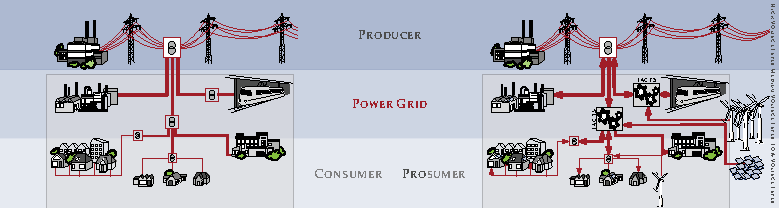
\includegraphics{intro/fig/power-grid-structure.pdf}%
    % 
    \caption[Change of the power grid hierarchical structure.]{Two exemplary
    power grids showing the conventional power grid (left) and the current
    development of the power grid (right). Both power grids consists of three
    voltage layers. On the~\myhl{KITseablue50}{high voltage layer} there are the
    conventional power plants (\eg, coal and nuclear power plants) as well as
    bigger collections of wind farms and~\acrlong{vpp}s located. The industrial
    consumers are usually located on the~\myhl{KITseablue30}{medium voltage
    layer} that mainly presents a distribution layer. In
    the~\myhl{KITseablue15}{low voltage layer}, we have the households and small
    industrial consumers. Note that on the right side, participants of the last
    two layer might have photovoltaics and wind turbines and are thus denoted by
    the term \emph{prosumers} (\ie, acting as producer and consumer
    simultaneously).%
    }%
    % 
    \label{ch:intro:fig:power-grid-structure}%
\end{figure} 

Renewable energy producers are often added to the medium and low voltage layer
(\cref{ch:intro:fig:power-grid-structure} right side). This eventually causes a
bidirectional power flow which the conventional power grid was not designed for.
This change in the power grid usage might cause instabilities and new critical
lines. Critical lines represent lines, which removal might cause a blackout. The
idea of the latter problem is exemplary shown in~\parencite{Wit16}. Offshore
wind farms in the North and Baltic Sea
(see~\cref{ch:intro:fig:north-sea-wind-farms}) provide another example for such
producers. In this particular case, the suitability of a location for such farms
highly depends on the wind profile and available space. Thus, the location for
wind farms is not as flexible as for conventional power plants. These offshore
wind farms produce---similar to conventional power plants---a high amount of
electrical energy that is not used on-site. However, it is largely required in
areas such as the Ruhr region, and southern regions of
Germany~\parencite{online:europe:project132:hvdc-line-a-north,online:europe:project235:HVDC_SuedLink_Brunsbuettel_Wilster-to-Grossgartach_Grafenrheinfeld,online:europe:TYNDP-2018-Projects-Sheets-166,online:europe:north-south-interconnections},
since a large number of industrial consumers are located there. Sending such an
amount of energy through the power grid causes new bottlenecks or is simply
impossible. Switching these wind farms off to sustain the grid safety is not a
desirable solution. Thus, to cope with these new challenges
the~\acrlong{tso}~(\gls{tso}) can follow at least two possible strategies.
% 
\crefformat{enumi}{#2\textup{Strategy~#1}#3}
\begin{enumerate}[(S1)]
    % 
    \item The expansion of the power grid by adding new transmission lines and
    \label{ch:intro:strategy:1}
    % 
    \item the installation of advanced control units such as~\acrlong{facts} 
    (\gls{facts}) and switches for a better utilization of the existing power
    grid.
    \label{ch:intro:strategy:2}
    % 
\end{enumerate}
% 
The mentioned power grid structure and strategies lead to the~\emph{dynamic}
and~\emph{static transmission design problem}~\parencite{Bin01a}.
\textcite{Bin01a} consider~\cref{ch:intro:strategy:1} as dynamic transmission
design problems~\parencite{Gal92,Cho06,Bin01a} under which long-term power
grid configuration such as~\acrlong{tnep} (\gls{tnep}) is encountered.
\gls{tnep}~\parencite{Hem13} is the design problem of adding new 
transmission lines or circuits under different objectives such as the cost
minimization of the new added transmission lines or maximization of the
throughput of the power grid. Adding new transmission lines decreases the total
power grid resistance~\parencite{Cof14a}, which results in less energy losses.
However, adding lines can also decrease the operation limit---meaning the
throughput---of the power grid, which becomes more clear in~\cref{ch:switching}.
% 
\begin{figure}[t!]
    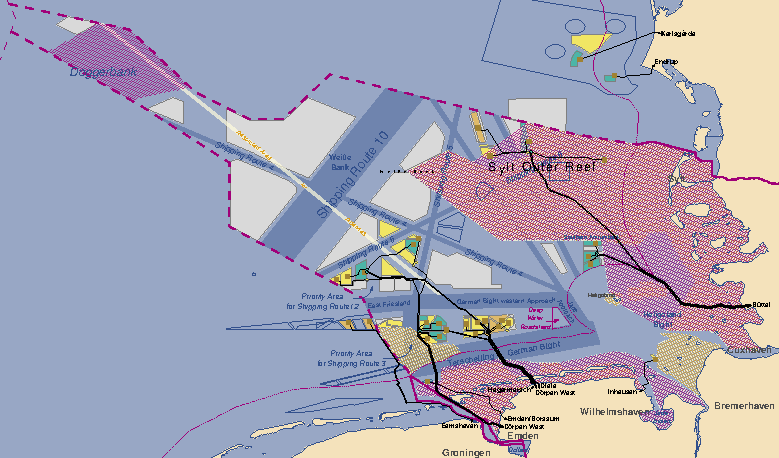
\includegraphics{windfarmplacement/figures/NorthSeaWindFarms.pdf}
    % 
    \caption[The offshore wind farms of the German Bight in the north sea.]{   
        The German offshore wind farms in the North Sea, where the
        \myhl{KITgreen50}{green}, \myhl{KITorange50}{orange}, \myhl{KITyellow50}
        {yellow}, and \myhl{KITblack15}{gray} areas represent wind farms that
        are \myhl{KITgreen50}{operating}, \myhl{KITorange50}{under
        construction}, \myhl{KITyellow50}{approved}, and \myhl{KITblack15}
        {planned}, respectively. There are many restricted zones that are
        prohibited for wind farm planning such as shipping routes, areas
        reserved for gas pipelines, \myhl{KITlilac30}{biota (violet hatched
        area)}, and \myhl{KITorange50}{bird sanctuaries (orange hatched area)}.
        A substation represents roughly speaking a collection point that
        collects the produced energy of wind turbines and forwards it. The
        connections from the last on-water substation to the first substation on
        the land-side (\eg, D{\"o}rpen West, Diele and B{\"u}ttel have
        substations) are usually implemented by~\acrlong{hvdc} (\gls{hvdc}).
        Note that this figure is a modification
        of~\parencite{online:offshore-wind-farm:german-bight}. }%
        % 
    \label{ch:intro:fig:north-sea-wind-farms}
\end{figure}
% 

Long-term power grid configuration has the major disadvantage that the planning
horizon is often in terms of
decades~\parencite{online:europe:TYNDP-2018-Projects-Sheets-166}, which is
counterproductive for the desired plan to change the power grid quickly in the
next few years~\parencite{online:eeg2014}. In addition, each expansion planning
is done for a certain topological scenario meaning a fixed power grid,
generation, and demand configuration. Different scenarios already occur with
different productions and consumptions. Thus, another strategy that covers
different scenarios and different topology changes is the placement of advanced
control units (\cref{ch:intro:strategy:2}). This is known as static design
problem, which is a subproblem of the dynamic design problem. The latter is less
cost intensive and represents a short-term configuration.

For~\cref{ch:intro:strategy:2} devices such as circuit breakers (known
as~\emph{switches}) and~\acrlong{facts} (\gls{facts}) are able to manipulate the
power flow by opening a circuit (switching a transmission line off) or rerouting
a certain fraction of power by changing the susceptance of a transmission line
in a device-specified interval, respectively. Both switches and~\gls{facts} are
able to reduce the generation cost while increasing the power grid operation
limit and satisfying the~$N-1$ criterion~\parencite{LiG13}. The~$N-1$ criterion
is a security and reliability criterion to ensure a stable operation while one
element is removed or has a failure. \textcite{Fis08} mentioned that switching
is already used by~\gls{tso}s in certain cases of emergency to decouple parts of
the grid, avoid abnormal voltage situations, or improve voltage profiles.
However, it is currently not used to extend the operability of the grid or
reduce costs and losses, since the~\gls{tso}s wish to interfere as little as
possible in the power grid to avoid instabilities.

Since power grids are one of the major backbones, their reliability is crucial.
A common and natural belief is that only~\gls{tnep} has the ability to maintain
and improve the reliability and operability of the power grid. However, placing
switches and~\gls{facts} is another way---though counterintuitive---to improve
the efficiency and reliability of the power grid. This counterintuitive behavior
is known as Braess's Paradox~\parencite{Bra68,Bra05} that is a common phenomenon
in many physical networks (see~\cref{ch:related-work:sec:braess-paradox}).
Furthermore, \textcite{Sch90} mentioned that both switches and~\gls{facts} have
the possibility to control over- and under-voltage situations, and line
overloads. Other papers confirm loss and cost reductions~\parencite{Sch90},
system security improvements~\parencite{Sch88}, and combinations of
all~\parencite{Hed11}.

In this work, we mainly focus on~\cref{ch:intro:strategy:2} by placing elements
such as switches or~\gls{facts} in such a way that we increase the operability
of the power grid and thus, the power grid's capacity. Note that increasing the
power grid capacity makes the power grid more reliable. Both electrical elements
can increase the maximum load. Switching provides a possibility to remove a
transmission line from the power grid temporarily. To the contrary, \gls{facts}
are control units that are able to influence the power flow in a certain range.
However,
\gls{facts} are also more expensive and complex. We will look
on~\cref{ch:intro:strategy:1} from the perspective of a plane grid with
generators and consumers, but no preinstalled interconnection. We motivate this
scenario by a wind farm planning problem denoted by wind farm cabling problem.
% 
%%%%%%%%%%%%%%%%%%%%%%%%%%%%%%%%%%%%%%%%%%%%%%%%%%%%%%%%%%%%%%%%%%%%%%%%%%%%%%%%
\section{Main Contributions}
\label{ch:intro:sec:contribution}
%%%%%%%%%%%%%%%%%%%%%%%%%%%%%%%%%%%%%%%%%%%%%%%%%%%%%%%%%%%%%%%%%%%%%%%%%%%%%%%%
% 
The contributions of this thesis are mainly covered by four parts. The first
part is about algorithms and structural results on electrical flows (also known
by the term~\emph{power flows}) and is called the~\acrlong{dc}~\acrlong{feas}.
The following two parts cover an overview of the results that concern the
efficient utilization of the existing power grid by placing switches (\ie,
discrete changes to the power grid) and~\acrlong{facts} (\gls{facts}; \ie,
continuous changes to the power grid), respectively. In the fourth part of this
work, the wind farm cabling results are outlined that
cover~\cref{ch:intro:strategy:1}.
%
%%%%%%%%%%%%%%%%%%%%%%%%%%%%%%%%%%%%%%%%%%%%%%%%%%%%%%%%%%%%%%%%%%%%%%%%%%%%%%%%
\paragraph{The Direct Current Feasibility Problem}
%%%%%%%%%%%%%%%%%%%%%%%%%%%%%%%%%%%%%%%%%%%%%%%%%%%%%%%%%%%%%%%%%%%%%%%%%%%%%%%%
% 
One main tool that we use in this thesis are electrical flows commonly known
under the term power flows. In this part, we will focus on the~\acrlong{dc}
\acrlong{feas} (\gls{dc}~\gls{feas}) that is an approximation of
the~\acrlong{ac}~\acrlong{feas} (\gls{ac}~\gls{feas})
(see~\cref{ch:foundations:sec:power-flow-analyses}). An algorithmic approach to
computing electrical flows will be our first contribution in this thesis and our
most fundamental result. We first give a mathematical description and structural
overview of the problem structure. This description is used to develop
algorithms for the electrical flow. One result shows that electrical flows do
not constitute~\acrlong{tum} (\gls{tum}) bases. However, we show a possible way
to solve the integer~\gls{dc}~\gls{feas}.

The first algorithm for~\gls{dc}~\gls{feas} is based on commonly known reduction
rules that will give us an algorithm that runs
in~$\bigO(\fmagnitude{\vertices}^3)$ time for an~\source-\sink planar power grid
(\ie, a power grid with one generator and one consumer). We give another
algorithmic idea for planar graphs that separates the quadratic relationship of
voltage and current by using two graphs and a mapping of their edges. In
addition to that, we are able to use a geometric interpretation of the problem
to improve the understanding for discrete and continuous changes. Note that for
linear systems the superposition principle holds in the physics and thus,
calculating~\gls{dc}~\gls{feas} for all generator and consumer pairs results in
an electrical flow for the whole power grid.
% 
% However, the last algorithm we
% develop is an efficient algorithm for the power flow calculation that runs
% in~$\bigO(\fmagnitude{\vertices})$ time on~\source-\sink power grid
% and~$\bigO(\fmagnitude{\vertices}^2)$ for general power grids.\franzi{Let's see
% if my intuition is correct}
%
%%%%%%%%%%%%%%%%%%%%%%%%%%%%%%%%%%%%%%%%%%%%%%%%%%%%%%%%%%%%%%%%%%%%%%%%%%%%%%%%
\paragraph{Discrete Changes in Power Grids}
%%%%%%%%%%%%%%%%%%%%%%%%%%%%%%%%%%%%%%%%%%%%%%%%%%%%%%%%%%%%%%%%%%%%%%%%%%%%%%%%
% 
The placement of switches represents a discrete change in the power grid and is
the first placement contribution we will focus on in this work. Note that a
discrete change represents a topology change. In particular, we address a
subproblem of the static design problem called~\acrlong{mtsfp}
(\acrshort{mtsfp}), which we model based on the~\acrshort{dc} electrical flow
(see~\cref{ch:switching:sec:model}). The problem's combinatorial nature makes it
hard to solve~\parencite{Leh14} and the current ways to tackle the problem are
exact but slow methods such as~\acrlong{milp}
(\acrshort{milp})~\parencite{Fis08} or even more complex
models~\parencite{6253283,HAGHIGHAT2015104}, or heuristics without provable
quality guarantees.
%
In contrast, we focus on structural properties and algorithms with provable
performance guarantees for the~\gls{mtsfp}. While it was known that~\gls{mtsfp}
is~\NP-hard in general~\parencite{Leh14}, we show that it is
% 
also~\NP-hard if the network contains only one generator and one consumer  
% 
(\source-\sink-networks). The latter is a generalization of another~\NP-hardness
proof given by~\textcite{Koc16}\footnote{We thank Thomas William Brown for
mentioning the paper of~\textcite{Koc16} to us after the conference talk of our 
paper~\parencite{Gra18}, since this work was not known to us.}.
For~\source-\sink-networks on restricted graph classes (including cacti) we
present an exact algorithm based on~\acrlong{dtp}{s} (\acrshort{dtp}s;
see~\cref{ch:switching:sec:exploit_structural_characteristics:subsec:dtp}).
These paths can be computed on general graphs and form the basis for a new
centrality measure resulting in a new algorithm that works well in practice.
% 
To the best of our knowledge, we are the first to provide an approximation and
an exact algorithm for~\gls{mtsfp} on special graph classes. Simulations on
the~\acrlong{nesta} (\gls{nesta}) benchmark set show that these algorithms
produce near-optimal results on most of the practical instances and thus, much
better solutions compared to the proven guarantee.
% 
%%%%%%%%%%%%%%%%%%%%%%%%%%%%%%%%%%%%%%%%%%%%%%%%%%%%%%%%%%%%%%%%%%%%%%%%%%%%%%%%
\paragraph{Continuous Changes in Power Grids}
%%%%%%%%%%%%%%%%%%%%%%%%%%%%%%%%%%%%%%%%%%%%%%%%%%%%%%%%%%%%%%%%%%%%%%%%%%%%%%%%
% 
Another way to use the grid more efficiently is by placing~\gls{facts}. Contrary
to switches that allow discrete changes, \gls{facts} represent a control unit
that change the electrical flow by scaling the susceptance. This represents
another static design problem and makes use of the existing power grid, too. We
assume that a flow control unit is an \emph{ideal}
\gls{facts}~\parencite{julieGriffin} controlling the electrical flow on its
branch without any restrictions. In the first work, we placed~\gls{facts} on
buses and in the follow-up, we considered ideal~\gls{facts} as elements that can
be only placed on branches. In general, the~\gls{facts} placement was shown to
be~\NP-hard~\parencite{Leh16}. Thus, most of the literature uses exact methods
such as~\acrlong{qp} (\acrshort{qp}) for the general formulation and for
ideal~\gls{facts} we will use an~\gls{milp}.

Using the well-known~\gls{ieee} power systems test
cases~\parencite{online:IEEEtestData,Zimmerman2011a,4075418,Bil70,online:TheUniversityOfEdinburgh:SchoolOfMathematics:PowerSystemsTestCaseArchive,
crow2015computational,Dem77,Gra03,780914,Jos16,6120344,5589973,4113721,Woo13},
we performed simulation experiments related to two key questions, which take
into account that the~\gls{facts} needed for implementing our flow control
vertices in the real power grid constitute a significant and expensive
investment and hence their number should be as small as possible. We investigate
the following two research questions. 
% 
% \crefformat{enumi}{#2\textup{Research Question~#1}#3}
\begin{enumerate}[(Q1)]
    \label{ch:intro:facts:researchQuestion}
    % 
    \item How many ideal~\acrshort{facts} are required and where do they have to
    be placed in order to obtain a lower bound for the operating costs?
    \label{ch:intro:question:numberFacts}
    %
    \item If the number of available ideal~\gls{facts} is given, do we still see
    a positive effect on the operating costs and on the operability of the grid
    during peak periods of the~grid?
    \label{ch:intro:question:costsOperability}
    % \item We consider the state of the grid, where the branch limits are approached
    % and ask whether a limited number of flow control units can decrease the
    % operation costs and extend the grid operability?
    % 
\end{enumerate}
% 
In our simulations we determine the minimum number of flow control units
necessary to achieve the same solution quality as in a power grid in which each
element is controllable and which clearly admits a best bound on what can be
achieved with the network topology. Interestingly, it turns out that a
relatively small number of ideal~\gls{facts} are sufficient for this. In fact,
we can prove a theorem stating a structural graph-theoretic property, which, if
met by the placement of flow control units, implies the optimality of the power
flow and serves as a theoretical explanation of the observed behavior. Research
Question~\ref{ch:intro:question:numberFacts} becomes increasingly relevant as
the consumption of electrical energy grows faster than the grid capacities.
The~\acrlong{opf} (\gls{opf}) minimizes the total generation costs of the power
grid while maintaining a feasible electrical flow. Our experiments indicate that
installing few ideal~\gls{facts} in a power grid is sufficient not only to
achieve lower costs compared to an~\gls{opf} solution, but also allows to
operate the grid at capacities for which no feasible~\gls{opf} solution exists
any more.
% 
%%%%%%%%%%%%%%%%%%%%%%%%%%%%%%%%%%%%%%%%%%%%%%%%%%%%%%%%%%%%%%%%%%%%%%%%%%%%%%%%
\paragraph{Transmission Network Expansion Planning on the Green Field}%
%%%%%%%%%%%%%%%%%%%%%%%%%%%%%%%%%%%%%%%%%%%%%%%%%%%%%%%%%%%%%%%%%%%%%%%%%%%%%%%%
% 
Wind farms are an important and powerful possibility to convert wind into
electricity. There are different challenges that come with the planning of wind
farms such as the placement of turbines, the configuration/profile of turbines
and substations, and the cabling of turbines. The configuration of the whole
farm is computationally too expensive and even the cabling with multiple cable
types is in general~\NP-hard (see~\cref{ch:related-work:sec:wind-farm-cabling}).
To solve this~\NP-hard problem, we use a heuristic approach called Simulated
Annealing (see~\cref{ch:wfcp:sec:simulated-annealing}). We structure the problem
into multiple layers that decrease the overall complexity of the problem. The
problem is decomposed into circuits, substation problem, and full wind farm
cabling problem. We created a first openly available wind farm benchmark set
that is generated randomly and therefore is less structured than the standard
wind farm.
% 
%%%%%%%%%%%%%%%%%%%%%%%%%%%%%%%%%%%%%%%%%%%%%%%%%%%%%%%%%%%%%%%%%%%%%%%%%%%%%%%%
\section{Thesis Outline}
\label{ch:intro:sec:outline}
%%%%%%%%%%%%%%%%%%%%%%%%%%%%%%%%%%%%%%%%%%%%%%%%%%%%%%%%%%%%%%%%%%%%%%%%%%%%%%%%
% 
We give a brief overview of the organization of this thesis. In particular, we
would like to emphasize that parts of this thesis appeared in previously
published proceedings, and reports~\parencite{Lei15b,Lei15,Mch15,Leh17,Gra18}.
% 
\begin{description}
    \item[\cref{ch:related-work}] To understand the state of the art, we give a
    literature overview that is related to our research and differentiate our
    work to the known literature. In the beginning, we give a short summary on
    results concerning (electrical) flows and the development of digital
    techniques to compute such flows. A synergy of techniques known from
    graph-theoretical and power grid analysis is given
    in~\cref{ch:related-work:sec:analyses} that will provide us with techniques
    to understand and analyze power grids. Since our focus is on combinatorial
    problems in power grids, we describe the paradox
    (see~\cref{ch:related-work:sec:braess-paradox}) that makes switching a
    possible way to extend the operability of the power grid. Note that a
    similar effect is observed with~\gls{facts}. We show that there are works
    describing the Braess's Paradox not only for power grids and present known
    theoretical results. As already mentioned, switching increases the
    operability of the power grid. In~\cref{ch:related-work:sec:switching}, we
    give an overview of known techniques to tackle the switching problem and
    show how we classify our work in the current literature. We analyze similar
    things for the~\gls{facts} placement in~\cref{ch:related-work:sec:facts} and
    for the wind farm cabling problem
    in~\cref{ch:related-work:sec:wind-farm-cabling}.
    % 
    \item[\cref{ch:foundations}] In this chapter, we introduce basic terms and
    notions that will be used in this thesis with regards to graph theory
    (see~\cref{ch:foundations:sec:graph-theory}), graph-theoretical flows
    (see~\cref{ch:foundations:sec:graph-theoretical-flows}), and electrical 
    flows (see~\cref{ch:foundations:sec:power-flow-analyses}). For the two
    latter sections, we define the feasibility problems and show the
    relationships between the different models.
    In~\cref{ch:foundations:sec:power-flow-analyses}, we do not only define the
    feasibility problems, but give a broad overview of the models, describe the
    assumptions, advantages and disadvantages of certain model assumptions as
    well as common problems and the complexity of the power flow analysis. 
    % 
    \item[\cref{ch:network-analysis}] To analyze networks, we describe
    that the electrical flow (see~\cref{ch:foundations:sec:power-flow-analyses})
    is a subproblem of many problems that optimize and analyze power grids. In
    the literature overview, we commonly see the usage of the mathematical
    formulation that is solved using a solver such as Gurobi~\parencite{gurobi}.
    However, in this chapter, we analyze the mathematical structure of
    the~\acrlong{dc} \acrlong{feas}. We develop some algorithms for the~\gls{dc}
    electrical flow using the developed structural knowledge of the problem and
    show that the matrices are separately~\acrlong{tum} (\gls{tum}). The whole
    system is not~\gls{tum}. The first algorithm is based on contraction rules
    with worse runtime than solving the system of linear equations of the
    mathematical formulation. Using a reformulation of the electrical flow, we
    are able to design another algorithmic approach that is much simpler.
    % 
    \item[\cref{ch:switching}] This chapter is published in~\parencite{Gra18}.
    Switching is one of the problems that show the existence of Braess's
    Paradox. We classified our work already
    in~\cref{ch:related-work:sec:switching}.
    % 
    % In~\cref{ch:related-work:sec:switching}, we classify our technique in the
    % context of related problems such as~\acrlong{ots} (\gls{ots}) and the
    % existing approaches to tackle this problem. 
    % 
    A fundamental problem definition of~\acrlong{otsp} (\gls{otsp})
    and~\acrlong{mtsfp} (\gls{mtsfp}) is given in~\cref{ch:switching:sec:model}
    describing the relationships between different problems. Several
    transformations of the network model are introduced
    in~\cref{ch:switching:sec:network_modeling}.
    In~\cref{ch:switching:sec:exploit_structural_characteristics}, we describe
    algorithms and structural properties of switching
    % 
    on~\source-\sink-networks as well as showing when it becomes~\NP-hard. A
    2-approximation on special graph structures is provided
    in~\cref{ch:switching:sec:approximation_algorithm_on_cacti}.
    In~\cref{ch:switching:sec:evaluation}, we evaluate our algorithms with
    methodical extensions. We conclude our work
    in~\cref{ch:switching:sec:conclusion} by summarizing the obtained results
    and outline future work including open problems.
    % 
    \item[\cref{ch:facts}] This chapter is published
    in~\parencite{Mch15,Lei15,Lei15b}. Whereas switching represents a discrete
    change in the power grid, \gls{facts} allow a change of the electrical flow
    within an interval by scaling parameters such as the susceptance. Thus, it
    represents another possibility to \textquote{rebalance} the electrical flow
    by changing line parameters that have temporary influence on the topology of
    the power grid. In this chapter, we show that \gls{facts} as well as
    switches are able to increase the operability of the power grid, while
    decreasing the overall generation costs. In addition, we give theoretical
    evidence that certain graph structures provide an optimal electrical flow
    that is equivalent to the min-cost flow.
    % 
    \item[\cref{ch:wfcp}] This chapter is
    published in~\parencite{Leh17}. A fundamental problem definition for the
    wind farm cabling problem is given in~\cref{ch:wfcp:sec:model}, where we
    introduce a first formal hierarchical structure definition of the wind farm
    problem; we further differentiate the full farm problem into the substation
    and circuit problem. The basic simulated annealing algorithm is introduced
    in~\cref{ch:wfcp:sec:simulated-annealing} and we give our methodical
    extensions to this algorithm for the wind farm cabling problem.
    In~\cref{ch:wfcp:sec:sec:simulations}, we evaluate our algorithm by using
    generated graphs as benchmark set. These benchmark sets are often harder
    than the current real world wind farms. We conclude our work
    in~\cref{ch:wfcp:sec:conclusion} by summarizing the obtained results and
    outline future work.
    % 
    \item[\cref{ch:conclusion}] This chapter summarizes the work we have done on
    the previously introduced placement problems in power grids that can
    influence the effect of the Braess's Paradox and thus, are able to improve
    the efficiency of power grids. However, this work is just a start to look at
    these problems from an algorithmic point of view and a lot of further
    investigations are necessary to improve existing algorithms and to
    understand these problems in more detail. Some ideas for possible future
    investigations are outlined in this chapter.
\end{description}

%%%%%%%%%%%%%%%%%%%%%%%%%%%%%%%%%%%%%%%%%%%%%%%%%%%%%%%%%%%%%%%%%%%%%%%%%%%%%%%%
\Chapter{Literature Overview}{}{}
\label{ch:related-work}
%%%%%%%%%%%%%%%%%%%%%%%%%%%%%%%%%%%%%%%%%%%%%%%%%%%%%%%%%%%%%%%%%%%%%%%%%%%%%%%%
% 
In this chapter, we give a literature overview of the state of the art that is
relevant for this thesis. We start with a brief literature summary with regards
to (electrical) flows. Note that we will discuss (electrical) flows formally in
more detail in~\cref{ch:foundations}. For now it suffices that an electrical
flow represents some physical flow that differs from a graph-theoretical flow in
the sense that it has some (roughly speaking) balancing properties that makes it
inefficient in most cases with regards to optimization criteria that we focus on
(\eg, maximizing the throughput). However, it reduces the overall energy loss
(see~\cref{ch:network-analyzes:eq:minimize-losses-quadratic-eq}) making it more
energy efficient. In addition, there are different approximation levels for
electrical flows that are used for certain scenarios, which we discuss in more
detail in~\cref{ch:foundations}. A common way to calculate electrical flows is
by using solvers that search for a feasible solution. However, this gives us
very little structural insights in how electrical flows work and thus, we give
an overview of common reduction and transformation rules from the literature
in~\cref{ch:related-work:sec:analyses} that make use of the superposition
principle for linear systems. Note that we use the term network analysis in the
context of calculating an electrical flow by using techniques that give more
insights into the problem structure.
% 
There is currently not much known about structural insights to solve electrical
flows using algorithms. We only found reduction and transformation rules that are
not much investigated for a more complex power grid analysis. The only problem
specific algorithm known is an exponential time
algorithm~\parencite{Ses61,Sha87}. 

A major contribution of this work are placement problems. Placement problems
exploit the structure in the sense that they modify the electrical flow such
that some objective is optimized such as the throughput. This optimization is
possible since the electrical flow has the property of balancing itself and
thus, does not represent the best possible flow for a given topology. A
literature overview on the behavior of electrical flows and the placement
problems we focus on is given in~\cref{ch:related-work:sec:braess-paradox}. For
the placement problems, we distinguish between discrete
(see~\cref{ch:related-work:sec:switching}) and continuous placement problems
(see~\cref{ch:related-work:sec:facts}), on which we give literature overviews by
considering the placement of switches and~\acrlong{facts} (\gls{facts}),
respectively. For transmission network expansion planning, we will focus on
literature for the wind farm planning with the focus on wind farm cabling
in~\cref{ch:related-work:sec:wind-farm-cabling}. In this literature overview, we
will see that there is little known about the problem with regards to structural
results. Since there are not a lot of structural results, there are not a lot of
algorithms to tackle electrical flows and because of that to tackle the
aforementioned placement problems using algorithms.
% 
%%%%%%%%%%%%%%%%%%%%%%%%%%%%%%%%%%%%%%%%%%%%%%%%%%%%%%%%%%%%%%%%%%%%%%%%%%%%%%%%
\section{Graph-theoretical Flows and Electrical Flows}
\label{ch:related-work:sec:gt-flows-power-flows}
%%%%%%%%%%%%%%%%%%%%%%%%%%%%%%%%%%%%%%%%%%%%%%%%%%%%%%%%%%%%%%%%%%%%%%%%%%%%%%%% 
% 
The graph-theoretical flow complies with the conservation of flow meaning that
the incoming flow is equal to the outgoing flow. This is similar to the
principle of conservation of energy. If maximized it is called~\acrlong{mfp}
(\gls{mfp};
\cref{ch:foundations:sec:graph-theoretical-flows:para:maximum-flow-problem}). If
each edge has a cost function, the problem of minimizing the total cost is
called~\acrlong{mcfp} (\gls{mcfp};
\cref{ch:foundations:sec:graph-theoretical-flows:para:minimum-cost-flow-problem}).
Both optimization variants are well known problems with efficient algorithms for
both~\gls{mfp}~\parencite{Gol14}
and~\gls{mcfp}~\parencite{Gol89,Edm72,Kle67,Orl97,Gol90}. The graph-theoretical
flow complies with the conservation of flow (\ie, incoming is equivalent to the
outgoing flow at each vertex) and the capacity constraints at each edge.
However, electrical flows that we also call \emph{power flows} have to obey some
physical laws. The physical relationship between current, voltage, and
resistance was first formalized by~\textcite{Kir47} in~\acrlong{kvl} (\gls{kvl})
and \acrlong{kcl} (\gls{kcl}). The latter is equivalent to the flow conservation
of graph-theoretical flows. The~\gls{kvl} represents a conservation of flow on
cycles and not on vertices. The latter law states that the flows in a cycle
(also known as mesh) sum up to zero. A base is a maximum independent set.
\citeauthor{Kir47} introduces for the~\gls{kvl} the concept of cycle bases,
which we will discuss in more detail in~\cref{ch:network-analysis}. He shows
which equations form a cycle base (\ie, a number of equations that suffice to
compute the~\gls{kvl}), and he reformulates the voltage law in terms of a cycle
base. This basically means that the number of equations for the~\gls{kvl} is
reduced from potentially exponentially many equations to polynomially many
equations while assuming simple graphs. Later, \textcite{Max65} describes the
electrical charge, electrical current, electrical field and magnetic field in
more detail. These works formalize the operation of power grids and thus, build
the foundation that is used in the power flow literature.
 
\paragraph{(Optimal) Electrical Flow Solution Techniques} 
% 
In the aforementioned paragraph, we described that an electrical flow complies
with the~\gls{kcl} and~\gls{kvl}. These laws constrain the electrical flow. A
usual question in power grids is if the demand can be fulfilled with the
currently available generation. This problem is called~\acrlong{feas}
(\gls{feas}). If we constraint the flow with the~\gls{kcl} and~\gls{kvl} law, we
call it the electrical flow feasibility problem. We will see
in~\cref{ch:foundations:sec:power-flow-analyses} that there are different
approximations for electrical flow and thus, different feasibility problems. In
the following, we will give a brief overview of existing solution techniques for
electrical flow feasibility problems in general. We will also mention the
\acrlong{opfp} (\gls{opfp}) that is an optimization problem that minimizes the
generation costs while complying with an electrical flow (here called power
flow).

There are different techniques to solve electrical flow feasibility problems.
One of the first surveys outlines digital techniques to solve the electrical
flow~\parencite{Sas67}. Another survey of electrical flow and optimal electrical
flow solution techniques is given by~\textcite{Huneault1991} outlining the first
automated digital solution technique by~\textcite{War56}, and the Gauss-Seidel
method introduced by~\citeauthor{Car62}~\parencite{Car62,Car79}, that is later
replaced by the Newton-Raphson method~\parencite{Pes68,Cos99}.
% 
% \citeauthor{Car62} also
% introduced the first~\acrlong{opf} (\gls{opf}) formulation.

The problem of generating the required amount of power while obtaining minimum
operation cost is called \emph{\acrlong{edp}} (\gls{edp}).
% 
% For the classical~\gls{edp} a integer non-linear program
% needs to be solved, which is~\NP-hard~\parencite{Jue10b}. 
% 
To cope with the~\gls{edp} while incorporating an electrical flow feasibility
problem is called the~\acrlong{opfp} (\gls{opfp}) that was introduced
by~\textcite{Car62}. The development of solution techniques on~\gls{opfp} is
summarized by~\textcite{SurveyOPF1,SurveyOPF2}.

\textcite{Sto74} reduces the memory consumption and running time for electrical
flow feasibility problems by introducing sparsity techniques for the admittance
matrix and compares it to other methods. The idea behind the approach
of~\citeauthor{Sto74} is that the power grid has a very sparse network
structure~\parencite[p.17]{Cai12} and thus, techniques that exploit the sparsity
improve the running time and memory consumption. A comparison of different power
formulations (see~\cref{ch:foundations:sec:power-flow-analyses:subsec:AC-Model})
is given by~\textcite{Cos08}. \textcite{Mol19} give a survey of relaxations and
approximations of the electrical flow equations.
In~\cref{ch:related-work:sec:analyses}, we outline some literature that mention
possible ways to analyze power grids. Note that as far as we know there is no
\textquote{purely} algorithmical approach to solve the power flow problem apart
from an exponential time algorithm~\parencite{Ses61,Sha87}. For linear systems
there are reduction and transformation rules known, which are not used so far to
create an algorithm for electrical flows. A literature overview including known
applications of these rules is given in the following.
% 
% The first method used for the AC load flow analyses was the also the
% Gauss-Seidel method.
% 
% - slow because of slow convergence~\parencite[p. 71]{wood1996power}
% - difficulties with negative reactance branches
% - each bus is treated independently
% -> each correction to one bus requires changes to the other buses
% 
% Another possibility to solve the problem is the newton-raphson method 
% based on the idea to calculate the correction (take all interactions into
% account) [reformulate]
% 
% Afterwards 
% - 1929 pf solved with analog network analyzern
% - Lagrangian techniques for the optimality cond. but neglegts variable bounds 
% (Squires 61)
% - Carpentier - optimality conditions for the OPF incl. variable bounds 
% (Kuhn-Tucker-Conditions) + first fully formulated OPF
% 
%%%%%%%%%%%%%%%%%%%%%%%%%%%%%%%%%%%%%%%%%%%%%%%%%%%%%%%%%%%%%%%%%%%%%%%%%%%%%%%%
\section{Reduction Rules for the Analysis of Power Grids}
\label{ch:related-work:sec:analyses}
%%%%%%%%%%%%%%%%%%%%%%%%%%%%%%%%%%%%%%%%%%%%%%%%%%%%%%%%%%%%%%%%%%%%%%%%%%%%%%%%
% 
\begin{figure}
    % 
    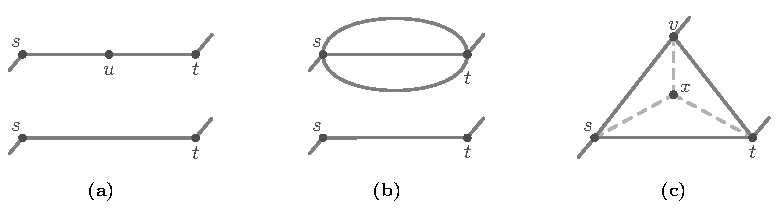
\includegraphics{relatedwork/figures/transformation.pdf}
    % 
    \caption[Common network reduction rules.]{Three different
    subgraphs that lead to different transformation rules each. These common
    transformation rules provide possibilities to reduce the network size. (a)
    In a series contraction a path with vertices of degree two can be contracted
    to a single edge. (b) In a parallel contraction multiple parallel edges can
    be contracted to a single edge. (c) The~\glssymbol{deltawye}-transformation
    (\glslongform{deltawye}; respectively \glssymbol{wyedelta}-transformation
    known as~\glslongform{wyedelta}) represent a possibility to increase
    (respectively decrease) the number of vertices and reduce (respectively
    increase) the number of triangles by one.
    % 
    }
    % 
    \label{ch:realted-work:fig:transformation}
\end{figure}
% 
In this work, we focus on a linear approximation of the electrical flow. Thus,
all equations, constraints, and objectives are linear functions. The goal of the
network analysis is to design algorithms that exploit the structure of the
problem such that these algorithms run in polynomial time in the input size.
There are different possibilities to analyze power grids. The common way to
compute electrical flows is to solve a set of linear equations using solvers
such as the~\gls{gurobi}~\parencite{online:Gurobi,gurobi}. However, the input
size has often a big influence on the running time to solve a problem. A
possibility to reduce the input size is to use reduction rules. However,
reduction rules in power grids include contraction and transformation rules.
Contraction rules are series
(see~\cref{ch:realted-work:fig:transformation}\screen{a}) and parallel
contractions (see~\cref{ch:realted-work:fig:transformation}\screen{b}) and
transformation rules are~\glssymbol{deltawye}- (\glslongform{deltawye}) and
\glssymbol{wyedelta}- (\glslongform{wyedelta}) transformations
(see~\cref{ch:realted-work:fig:transformation}\screen{c}). The latter rule
transforms a triangle to a star by adding one vertex into the center and adding
edges from the center to the already existing vertices, while removing the
original edges, and vice versa for the inverse transformation, respectively. The
generalization of the \glssymbol{deltawye}-
and~\glssymbol{wyedelta}-transformations are the star-mesh- (or star-polygon-)
transformations~\parencite{Lie73,Bed61}. Other common rules are self-loop and
degree-1 removals.

These reduction rules are applied on different problems in different fields of
research such as in statistical physics involving the evolution of crystal
lattice energy~\parencite{Bax16}, network
reliability~\parencite{Leh63,Sat93,Tra02}, knot theory~\parencite{Rei83,Tra02},
and graph theory~\parencite{Ake60,Cha17}. We start with some initial algorithmic
results on the transformation rules in the following.

\paragraph{Reducibility of Graphs and Complexity of Reduction Algorithms}
% 
The first more general structural observations concerning reduction rules are
by~\textcite{Ake60} and~\textcite{Leh63}. Both independently introduce the
conjecture that by using a combination of~\glssymbol{wyedelta}-
and~\glssymbol{deltawye}-transformations, as well as series and parallel
contractions the connected, two-terminal, undirected, planar graph can be
reduced to a single edge connecting the given
terminals~\parencite[pp.795ff.]{Leh63}. The latter conjecture is then
independently proven by~\textcite{Gru03} using a graph without terminals, and a
complicated and non-constructive proof by~\textcite{Epi66}.
Using~\glssymbol{deltawye}-
and~\glssymbol{wyedelta}-transformations~\citeauthor{Epi66} proves that any
polyhedral graph (\ie, an undirected graph that is a representation of a convex
polyhedron) can be reduced to a~$K_4$ (\ie, complete graph with four vertices).
The proofs of the conjecture is simplified by~\textcite{Tru89} using a
constructive proof incorporating graph minors. One major property used
in~\citeauthor{Tru89}'s proof is that planar graphs can be embedded as grid
graphs. \citeauthor{Tru89} provides a much simpler polynomial time algorithm for
planar graphs than the one by~\textcite{Feo85}.
\citeauthor{Tru89}'s~\parencite{Tru89} algorithm
requires~$\bigO(\fmagnitude{\glssymbol{vertices}}^2)$ space, but he did not
mentioned the running time of the algorithm. However, \textcite{Feo85} designed
a more complex algorithm that runs
in~$\bigO(\fmagnitude{\glssymbol{vertices}}^2)$ time and
needs~$\bigO(\fmagnitude{\glssymbol{vertices}})$ space. \textcite{Val79} showed
that the series, parallel, loop, and single degree reductions for
series-parallel-graphs can be done in~$\bigO(\fmagnitude{\glssymbol{vertices}})$
time. In addition, \textcite{Pol83} showed that every~\gls{wyedeltagraph} (\ie,
a graph that can be reduced to a vertex by the aforementioned reduction rules)
is planar. The term~$C_i$ (also known as~$i$-cyclic graph) represents a closed
walk of length~$i\in\naturals$ with~$i$ being the number of vertices. A planar
graph is a~\gls{wyedeltagraph} if and only if it is a~$(C_5+2K_1, K_2\times
C_4)$-free graph~\parencite{Pol83} or~$(K_5, K_{2,2,2}, C_8(1,4), K_2\times
C_5)$-free graph~\parencite{Arn90,Sat90}, respectively. To the extent of our
knowledge, it is unknown whether these algorithms are applicable to power grids
or not. Some application to graph-theoretical problems are given in the next
paragraph.
% 
\paragraph{Preservation of Optimization Properties}
% 
Regardless of the structural point of view, these transformations are used when
solving algorithmic problems. 
% 
Dependent on the problem, it is necessary to show that the transformation and
contraction rules preserve a solution space. This is roughly done
by~\textcite{Ake60} for the~\acrlong{mfp} (\gls{mfp}) and~\acrlong{sppp}
(\gls{sppp}).
% 
He used the transformations to simplify the network such that algorithmic
problems become easier to solve. \textcite{Ake60} applied the transformations to
solve~\gls{sppp} and~\gls{mfp} on undirected~$2$- and~$3$-terminal graphs while
preserving the optimal length or flow value. Interestingly, the transformations
shown in~\textcite{Ake60} also behave dually meaning that, \eg, the calculation
of the capacities of the series reduction is the calculation of the parallel
reduction in the dual problem. The duality of the transformations is shown
for example in~\textcite{Ake60}. Another work by~\textcite{Cha17} uses these
reduction rules to untangle planar curves meaning to simplify a planar graph
with a certain number of self-crossings. In the next paragraph, we show the
usage of the reduction rules with regards to network reliability. Within network
reliability there is a lot of literature available that gives structural results
on the hardness of the problem and uses methodology to tackle~\NP-hard problems,
which we will use for some placement problems.
% 
\paragraph{Preservation of Network Reliability}
% 
In network reliability these reductions rules are used extensively. Network
reliability studies the probability that at least one path connecting two
terminals operates successfully. The edges in such a network have success
probabilities. The problem of computing the all-terminal reliability for
arbitrary networks is known to be~\NP-hard~\parencite{Pro83,Val79a}. The hardness
remains even for planar graphs~\parencite{Ver05}. 
% 
% Application of the all-terminal reliability are given
% in~\parencite{Pol83,Pol90,Arn90,el1990two}
% \franzi{check again}. 
% 
\textcite{Leh63} showed that series, parallel, degree-1, and loop reductions
preserve reliability in the two-terminal and undirected network case. The
\glssymbol{deltawye}- and \glssymbol{wyedelta}-transformations for boolean functions
(also known as switching-functions) are introduced by~\textcite[Section
4]{Leh63}. However, he shows that these transformations do not calculate the
exact probability, but an approximation to it.
% 
% He used numerical transformation tables since the values were between~$0$
% and~$1$. 
% 
Since the problem is in general~\NP-hard, \textcite{Sat93} developed efficient
algorithms for special graph classes, which run
in~$\bigO(\fmagnitude{\glssymbol{vertices}}\log\fmagnitude{\glssymbol{vertices}})$
time.
% 
% , where~\glssymbol{vertices} represents the set of buses. 
% 
The latter work~\parencite{Sat93} uses the technique of forbidden minors (\ie, a
minor~\minor is a graph that can be extracted from a graph~\glssymbol{graph} by
applying vertex and edge deletions and edge contractions) to develop efficient
algorithms for reliability analysis on graph subclasses. \citeauthor{Sat93} not
only focused on the two terminal case, but on the $K$-terminal reliability that
focuses on the probability that there is a path between every pair of terminals.
Where~\textcite{Leh63} showed that not all transformations are reliability
preserving reductions, \textcite{Sat93} focused on reliability preserving
reductions and introduced a
\gls{trisubgraph}-Y-reduction. They focused on block-cut-trees, $3$-connected
graphs, and series-parallel graphs. For the latter graph structure they observed
that it depends on the distribution of the terminals whether the graph is
reducible or irreducible and thus, reliability preserving using the standard
reduction rules or not. The $K$-terminal reliability on
series-parallel-reducible networks can be computed
in~$\bigO(\fmagnitude{\glssymbol{edges}})$ time using series, parallel,
degree-1, and -2 contractions~\parencite[pp.827ff.]{Sat85}. However, for
series-parallel-irreducible graphs these reduction rules are not sufficient and
thus, \textcite{Sat85} designed a linear time algorithm using
the~\emph{polygon-to-chain reduction} that reduces two parallel
paths~$\fpath{1}{\source}{\sink}$ and~$\fpath{2}{\source}{\sink}$ with inner
vertices of degree-2 to one path having a length of $\max\{
\fmagnitude{\fpath{1}{\source}{\sink}},
\fmagnitude{\fpath{2}{\source}{\sink}} \}$. For basically series-parallel
directed graphs (\ie, graphs where the underlying graph is a series-parallel
graph)~\textcite{Agr84,Agr85} provide an $\bigO(\fmagnitude{\glssymbol{edges}})$
time algorithm to compute source-to-K-terminal reliability.
\textcite{Pol86,Pol90} show that for~$K_2\times C_4$-free graphs the reliability
can be computed in linear time and~\textcite{Pol92} show that the all-terminal
reliability of a~$(K_5, K_ {2,2,2})$-free graph can be computed
in~$\bigO(\fmagnitude{\glssymbol{vertices}}\log\fmagnitude{\glssymbol{vertices}})$
time. \textcite[p.13; Proposition~2]{Sat93} show that a~\gls{wyedeltagraph}
allows a~\gls{trisubgraph}-Y reduction resulting in a~\gls{wyedeltagraph}.

\paragraph{Further Results}
% 
There are results on reducibility for planar graphs, non-planar graphs, and
special graphs that we outline here. \textcite{Git91} proofs for reducibility
for graphs with no~$K_5$ minor and graphs with no~$K_{3,3}$ minor. The
reducibility for projective-planar graphs (\ie, a projective plane is an
extension of the euclidean space, where parallel edges intersect in a point and
thus, all edges intersect in some point) and graphs with crossing number one was
shown by~\textcite{Arc00}. For 4-terminal reducibility of planar graphs,
\textcite{Demasi:2015:FTP:2722129.2722244} show that a sufficiently
connected~\gls{cubicgraph} (\ie, a graph, where all vertices have a degree of
three) are reducible if and only if it does not contain a Petersen graph as
minor. Later \textcite{Wag15} presents a reducibility for almost-planar graphs
with the condition that all graphs in the reduction sequence remain
almost-planar. Other works define the reducibility with a set of forbidden
minors~\parencite{DBLP:journals/jgt/Yu04a,DBLP:journals/combinatorics/Yu06} and
design algorithm for 3-terminals, special cases of 4-terminal planar graphs,
$k$-cofacial terminals in planar graphs~\parencite{Git91,doi:10.1002/net.20399}.
% 
% \franzi{Read the work of~\citet{6316101} and incorporate it}
% 
%%%%%%%%%%%%%%%%%%%%%%%%%%%%%%%%%%%%%%%%%%%%%%%%%%%%%%%%%%%%%%%%%%%%%%%%%%%%%%%
% \begin{landscape}
%     \begin{table}
%         % 
%         % latex table generated in R 3.2.2 by xtable 1.8-0 package
% Wed Jan 27 11:17:04 2016
{\setlength{\tabcolsep}{0.3em}}
{\renewcommand{\arraystretch}{1}}% for the vertical padding
\small
% \begin{tabular}{p{2cm}p{3cm}p{3cm}p{3cm}p{3cm}p{3cm}}
\begin{tabular}{%
>{\centering\arraybackslash}m{3cm}%
>{\arraybackslash}m{2.5cm}%
>{\centering\arraybackslash}m{2cm}%
>{\arraybackslash}m{3.5cm}%
% >{\centering\arraybackslash}m{2cm}%
>{\arraybackslash}m{2cm}%
% >{\centering\arraybackslash}m{0.56cm}%
% >{\arraybackslash}m{2.3cm}%
% >{\centering\arraybackslash}m{0.56cm}%
% >{\arraybackslash}m{1.5cm}%
% >{\centering\arraybackslash}m{0.56cm}%
}%
% 
\toprule
  \multirow[c]{1}*{Graph Structure}     & 
  \multicolumn{1}{c}{Problem}           &
  \multicolumn{1}{c}{Complexity}        & 
  \multicolumn{1}{c}{Reduction Rules}   &
  % \multicolumn{1}{c}{Algorithm}         &
  \multicolumn{1}{c}{Cite}
  \\
%-------------------------------------------------------------------------------
%-------------------------------------------------------------------------------
% 
%-------------------------------------------------------------------------------
%-------------------------------------------------------------------------------
% 
%-------------------------------------------------------------------------------
%-------------------------------------------------------------------------------
 \midrule  
%-------------------------------------------------------------------------------
%-------------------------------------------------------------------------------
\rowcolor{Table-Line-Marker}
% 
    Arbitrary graphs 
    & All-terminal reliability 
    & \NP-hard 
    & -- 
    % & -- 
    & \parencite{Pro83,Sat90}
\\
    Planar graphs 
    & Reliability $R(\glssymbol{graph})$ 
    & \NP-hard 
    & -- 
    % & -- 
    & \parencite{Ver05} 
\\
\rowcolor{Table-Line-Marker}
% 
\rowcolor{Table-Line-Marker}
    Series-parallel reducible graph 
    & K-terminal reliability $R_K(\glssymbol{graph})$ 
    & $\bigO(\fmagnitude{\glssymbol{edges}})$ 
    & 
    \begin{tabular}[c]{@{}l@{}}
    Series, 
    \\ parallel, and 
    \\ degree-1
    \end{tabular} 
    % & -- 
    & -- 
\\
    Series-parallel irreducible graph 
    & K-terminal reliability $R_K(\glssymbol{graph})$ 
    & linear time 
    & 
    \begin{tabular}[c]{@{}l@{}}
        Polygone-to-chain, 
        \\ series, 
        \\ parallel, and 
        \\ degree-1
    \end{tabular} 
    % & -- 
    & \parencite{Sat85} 
\\
\rowcolor{Table-Line-Marker}
    Basically series-parallel digraph 
    & Source-to-K reliability
    & $\bigO(\fmagnitude{\glssymbol{edges}})$ 
    & -- 
    % & -- 
    & \parencite{Agr85} 
\\
    $K_2\times C_4$-free graph 
    & Reliability $R(\glssymbol{graph})$ 
    & linear time 
    & -- 
    % & -- 
    & \parencite{Pol83,Pol86} 
\\
% 
\rowcolor{Table-Line-Marker}
    $\Delta-Y$-graph 
    & Reliability~$R(\glssymbol{graph})$ 
    & $\bigO(\fmagnitude{\glssymbol{vertices}}^2)$ 
    & -- 
    % & -- 
    &  
\\
% 
    $(K_5,K_{2,2,2})$-free graph 
    & All-terminal reliability 
    & $\bigO(\fmagnitude{\glssymbol{vertices}}\log
    \fmagnitude{\glssymbol{vertices}})$
    & -- 
    % & -- 
    & \parencite{Pol92} 
\\
%--------------------------------------------------------------------------------------------------------------------------------------------------------------------------------------------------------------------------------------------------------------------
   \bottomrule
\end{tabular}%

%         % 
%         \caption[Overview of the results that make use of reduction rules.]
%         {Overview of the results that make use of reduction rules. This table
%         shows that different graph structures lead to different complexities.}
%         % 
%         \label{ch:switching:sec:complexity:tbl:complexity-overview}
%         % 
%     \end{table}
% \end{landscape}
%%%%%%%%%%%%%%%%%%%%%%%%%%%%%%%%%%%%%%%%%%%%%%%%%%%%%%%%%%%%%%%%%%%%%%%%%%%%%%%
% 
%%%%%%%%%%%%%%%%%%%%%%%%%%%%%%%%%%%%%%%%%%%%%%%%%%%%%%%%%%%%%%%%%%%%%%%%%%%%%%%%
\section{Braess's Paradox -- Effects that Influence the Power Grid Efficiency
and Stability}
\label{ch:related-work:sec:braess-paradox}
%%%%%%%%%%%%%%%%%%%%%%%%%%%%%%%%%%%%%%%%%%%%%%%%%%%%%%%%%%%%%%%%%%%%%%%%%%%%%%%%
% 
The main focus of this thesis is on placement problems with additional physical
properties. In the introduction (see~\cref{ch:intro}), we discuss two strategies
to improve the power grid efficiency. In contrast to our intuition, not only the
expansion of the power grid (\gls{tnep}; \cref{ch:intro:strategy:1}
in~\cref{ch:intro}), but also switching can be used to improve the efficiency of
the power grid. This implies that adding a new line to the power grid can also
decrease the throughput of the power grid or increase the overall generation
costs.

A similar phenomenon exists for road networks and is called Braess's
para\-dox \parencite{Bra68,Bra05}. Introducing a new road to the traffic network
might cause longer travel times~\parencite{You08}. The main reason is that every
participant wants to independently minimize its own travel time, while ignoring
the decision's effect on other travelers~\parencite{Pas97}. In addition,
\textcite{Pas97} show that the occurrence of the Braess's paradox highly depends
on the instance parameters, \ie, demand and congestion functions. Thus, the
paradox usually occurs within some bounds that make it possible that the network
might \textquote{grow in} and \textquote{grow out} of the paradoxical situation
with increasing (traffic) demand. 

\textcite{Coh91} describe the existence of the paradox in
mechanical~\parencite{Pet12} and electrical networks (for both
see~\parencite{Pen03}). Other works show that the paradox also appears in
oscillator networks~\parencite{Wit12}, where adding a line can cause
instabilities and even power outages, which confirms once more the existence of
the Braess's paradox in real power grids~\parencite[p.11]{Wit12}. Another
example for this exists in quantum physics~\parencite{Pal12}.

\textcite{Coh91} also emphasize the non-intuitive behavior of the Nash
equilibrium that arises in most physical networks. We know from~\textcite[p.4;
Section 3]{Dub86} that Nash Equilibria \textquote{tend to be inefficient in the
Pareto sense}. We will give an explanation of that
in~\cref{ch:network-analysis}. The Nash Equilibrium is a known fix point in Game
Theory and represents a state, where no player wants to change its choice. In
contrast, the Pareto optimum means that there is no possible better choice of
one player that does not decrease the payoff of another player. Thus, it is the
optimum with regards to a cost function. The Pareto front represents the set of
Pareto optima. However, the Pareto optimization plays a crucial role in the
multi-criteria optimization. We show an example for a Pareto front
in~\cref{ch:facts:sub:experiments-control-units:fig:plot-costs-losses}. An easy
example that shows Pareto optima and Nash Equilibriums is given
in~\textcite[p.5; Figures 2--4]{Dub86}.

Another theoretical insight given by~\textcite{Val06} explaining that the
Braess's paradox occurs very often in random graphs. Note that many of the
networks in the real world have properties similar to random
graphs~\parencite[p.xiii]{online:Hof19}. Thus, in~\cref{ch:switching}, we
exploit the Braess's paradox to improve the efficiency of the power grid,
whereas in the~\gls{tnep} problem, we have to add lines in a way that the
efficiency of the power grid increases and thus, the effect of the Braess's
paradox does not appear. The effect that the Braess's Paradox highly depends on
the instance parameters~\parencite{Pas97} is shown
in~\cref{ch:switching,ch:facts}, where we use switches and~\gls{facts} to
influence these parameters.
% 
%%%%%%%%%%%%%%%%%%%%%%%%%%%%%%%%%%%%%%%%%%%%%%%%%%%%%%%%%%%%%%%%%%%%%%%%%%%%%%%%
\subsection{Switching -- A Discrete Manipulation of the Power Grid Topology}
\label{ch:related-work:sec:switching}
%%%%%%%%%%%%%%%%%%%%%%%%%%%%%%%%%%%%%%%%%%%%%%%%%%%%%%%%%%%%%%%%%%%%%%%%%%%%%%%%
% 
Recall that switching is the process of temporarily removing a transmission line
from the power grid by using devices such as circuit breakers.
\citeauthor{Kir47} model this behavior by changing the resistance to
infinity~\parencite[p.501]{Kir47}.
% 
Switching was first analyzed as a negative effect in the power
grid~\parencite{GLAVITSCH198592} responsible for overloads, voltage drops, and
the loss of network stability.
%
\textcite{koglin1980overload} introduce transmission switching as a corrective
control action to reduce transmission line overloads. Later other positive
switching effects were recognized such as improving currents, decreasing loads
and angles, creating voltage drops, and changing the short-circuit
power~\parencite{GLAVITSCH198592,Hed11,744552}.

\textcite{1388507} and~\textcite{Fis08} introduce
the~\acrlong{otsp}~(\gls{otsp}) and its formulation based on
the~\acrlong{dcopf}~(\gls{dcopf})~\parencite{Cho06}, respectively.
The~\gls{otsp} using~\gls{dc}-constraints is called~\gls{dcots}.
\textcite{Fis08} observe that switching may improve the economic efficiency of
the~\acrlong{edp} (\gls{edp}). However, they could not find any general trend in
the physical characteristics of the switched lines.
%
Many models were presented that are more complex~\parencite{6646289,7285833} or
minimize either the
%
overload~\parencite{4334990,193839,486127},
% 
voltage problems~\parencite{4335192,ROLIM1995177},
% 
losses~\parencite{192895}, or 
% 
generation costs~\parencite{Fis08,ONeill2010}.
Others enhance the security~\parencite{Sch90,38969}, 
reliability~\parencite{6656013,7874194,7325581},
% 
economic seasonal~\parencite{6878486}, or 
% 
\acrlong{tnep}~(\gls{tnep}) costs~\parencite{5409537,VILLUMSEN2012377}.

\gls{dcots} is known to be~\NP-hard~\parencite{Leh14,Leh15a} 
% 
and solving it by running an~\acrlong{ilp} (\gls{ilp}) has impracticable running
times~\parencite{Fis08}. The complexity is reduced by limiting the solution set,
\ie, number of switches~\parencite{4558426,4957010,1525118}.
% 
Often a small number of switches is sufficient to reach the optimum. This is a
central property in most heuristics~\parencite{5463055,7038445,6164300} that use
a ranking of the transmission lines based on different criteria.
\textcite{7764208} show that switching lines with high congestion costs is a
reasonable criterion to reduce the overall cost. Other pre-screening techniques
rank the lines on their dual prices for each bus~\parencite{6191339}. Other
approaches are Evolutionary Algorithms~\parencite{916873,5352849},
branch-and-bound~\parencite{6955256}, and
partitioning~\parencite{7494647,LiG13,7038447}. \textcite{6938949} use a soft
rounding heuristic~\parencite[p.629]{Jue10aa} not fixing all variables to a
value but obtaining this by changing the objective function coefficient of the
binary variables.% , \ie, here an auxiliary induce function (AIF).

However, there is not a lot known with regards to structural exploits of the
power grid topology. \textcite{6169974,6799266} exploited the symmetry of
transmission lines for the switching problem by removing identical parallel
transmission lines. Different network parameters lead to a different system
performance and are connected in some sense to
switching~\parencite{BOMPARD20095,doi:10.1063/1.3077229,4438889}.
% 
{\hypersetup{citecolor=black}\citeauthor{6480106}}~\parencite{6069831,6480106,6039669} 
% 
use topological and electrical parameters as a heuristic. In addition, they
investigate parameters concerning~\gls{ots} such as resistance, reactance,
susceptance, vertex degree, thermal limits, and edge-betweenness
centrality~\cite{4438889} (number of shortest paths through an edge) but find no
statistically significant relationship.
% 
Recall that~\textcite{Pas97} show that the Braess's Paradox highly depends on
the instance parameters and that a single parameter evaluation lacks in this
particular case as it is influenced by multiple parameters such as
topology, susceptance, and capacity.
% 
In addition, there exist also screening and ranking systems based on network
flows~\parencite{4334990,486127}.

Most of the work so far tries to adapt~\gls{ots} to other problems, 
% 
reformulates the model, or analyzes it for different power grids. However, the
majority of the papers have problems to solve their models to optimality even on
small instances. Thus, most heuristics try to decrease the search space, a few
concentrate on structural aspects of power grids, while others try to find
correlations between power grid parameters and switching.
%
A common observation is that the effects of transmission switching are
relatively localized~\parencite{6069831,6039669,GLAVITSCH198592}. This
observation is debatable as it is made without solving the problem to optimality
and using test cases such as the \emph{reliability test system
1996}~\gls{rts}-96 test case that is three copies of the~24-bus power system 
linked together. However, in general there is no network property found to
distinguish the switched lines~\parencite{6039669}. Thus, current techniques do
not provide a deeper understanding of the problem structure. The latter will be
our contribution to the community for certain graph structures, which we give
in~\cref{ch:switching}.
% 
%%%%%%%%%%%%%%%%%%%%%%%%%%%%%%%%%%%%%%%%%%%%%%%%%%%%%%%%%%%%%%%%%%%%%%%%%%%%%%%%
\subsection{FACTS -- A Continuous Manipulation of the Power Grid Topology}
\label{ch:related-work:sec:facts}
%%%%%%%%%%%%%%%%%%%%%%%%%%%%%%%%%%%%%%%%%%%%%%%%%%%%%%%%%%%%%%%%%%%%%%%%%%%%%%%%
% 
Recall that the graph-theoretical flow is a flow mainly controlled by
the~\gls{kcl} and capacity constraints, whereas the electrical flow has to obey
physical laws. The graph-theoretical flow and the electrical flow give us, while
maximized (respectively when the generation cost is minimized), the upper and
lower bounds (respectively lower and upper bounds), respectively (more on that
in~\cref{ch:network-analysis}). In addition, \textcite{Pas97} show that
different instance parameters influence the effect of the Braess's Paradox.
Thus, changing the parameter helps to change the effect the Braess's Paradox has
on the network. With~\gls{facts} the idea is to exploit the network structure
such that the flow behaves more like a graph-theoretical flow and thus, closer
to the best bound. Recall that a similar approach is done by switching.

With the increasing availability and technological advancement of~\gls{facts}
researchers began to study the possible benefits of their installation in power
grids from different perspectives to approach the Research
Questions~\ref{ch:intro:question:numberFacts}--\ref{ch:intro:question:costsOperability}
(see~\cref{ch:intro:sec:contribution} on
Page~\pageref{ch:intro:facts:researchQuestion}).

From an economic perspective, it is of interest to support investment decisions
in power grid expansion planning by considering alternative investment
strategies that either focus on new transmission lines or allow mixed approaches
including~\gls{facts} placement. \textcite{bogr-rovfi-11} present a
least-squares Monte-Carlo method for evaluating investment strategies and argue
that~\gls{facts} allow for a more flexible, mixed strategy that fares
better under uncertainty. \citeauthor{ti-oidte-12} present an optimal
decision-making framework for comparing investment decisions,
including~\gls{facts}~\parencite{ti-oidte-12}.

From the perspective of operating a power grid, the main question is how many
ideal~\gls{facts} are required and where do they have to be placed in order
to optimize a certain criterion. \textcite{1397562} propose and experimentally
evaluate a genetic algorithm for allocating different types of~\gls{facts}
in a power grid in order to optimally support a deregulated energy market.
\textcite{gcg-olmtf-01} and~\textcite{1465551} study the placement
of~\gls{facts} with the goal of increasing the amount of energy that can be
transferred. \textcite{gcg-olmtf-01} present a genetic algorithm that
simultaneously optimizes the energy generation costs, transmission losses, line
overload, and the acquisition costs for~\gls{facts}. \textcite{1465551} use
evolutionary programming to place~\gls{facts} such that the total amount of
energy that can be transferred from producers to consumers is maximized. In
contrast to our setting, they may also increase the demands of consumers
arbitrarily. Contrary to these heuristic approaches~\textcite{lgkm-psp-03} use
mixed-integer linear programming to optimally increase the loadability of a
system by placing~\gls{facts} subject to limits on their number or cost.
Similar to our approach, they do not distinguish different types
of~\gls{facts} but rather assume \textquote{ideal}~\gls{facts} that
can control all transmission parameters of a branch.  However, they focus only
on loadability and do not consider generation costs and line losses. The latter
two objectives will be considered in our work.

All related work mentioned so far considers the~\gls{dc} model for electrical
networks as an approximation to the~\gls{ac} model (more on that
in~\cref{ch:foundations:sec:power-flow-analyses}) and aims at providing a
preliminary step in an actual planning process, where this approximation is
sufficient.  There are also a few attempts to solve the placement problem
for~\gls{facts} in the more realistic but also more complicated~\gls{ac}
models~\parencite{744495}. These models can be categorized as follows:
%
\begin{itemize}
    \item \gls{ac} models with sinusoidal loads (non-convex and non-linear
        formulation), 
    \label{ch:related-work:AC:1}
    % 
    \item \gls{ac} quadratic approximations (non-convex and quadratic
        formulation), 
    \label{ch:related-work:AC:2}
    % 
    \item \gls{ac} piece-wise-linearization (non-convex and integer linear
        programming formulation), and
    \label{ch:related-work:AC:3}
    % 
    \item \gls{ac} linearization (convex and linear formulation). 
    \label{ch:related-work:AC:4}
\end{itemize}
% 
\textcite{Sha03} develop an evaluation whether transmission lines are critical
and propose to place~\gls{facts} at critical lines in order to improve
voltage stability in the grid. \textcite{is-sonl-04} present a genetic algorithm
for~\gls{facts} placement in~\gls{ac} networks and experimentally
evaluate it in a case study. In contrast to these heuristic approaches,
\textcite{6507352} observe exact~\gls{opf} evaluation in a
relaxed~\gls{ac}-model. In this context, they place phase shifters to
exploit structural characteristics that are similar to our approach.
% 
%%%%%%%%%%%%%%%%%%%%%%%%%%%%%%%%%%%%%%%%%%%%%%%%%%%%%%%%%%%%%%%%%%%%%%%%%%%%%%%%
\section{The Wind Farm Cabling Problem}
\label{ch:related-work:sec:wind-farm-cabling}
%%%%%%%%%%%%%%%%%%%%%%%%%%%%%%%%%%%%%%%%%%%%%%%%%%%%%%%%%%%%%%%%%%%%%%%%%%%%%%%%
% 
\begin{figure}
    % 
    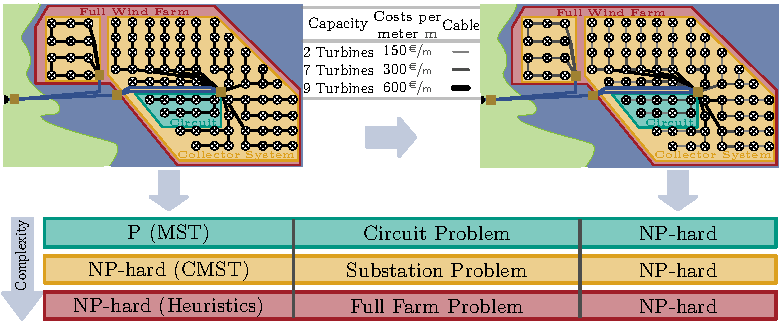
\includegraphics[page=1]{relatedwork/figures/windfarm-overview.pdf}
    % 
    \caption[The complexity of wind farm cabling problems.]{%
    The wind farm topology consists typically of turbines~\tikzTurbine and
    substations~\tikzSubstation. The complexity of cabling a wind farm differs
    depending on the cost function. If we assume unit costs---meaning we have
    only one cable type~\tikzOneTransportCable available---then the problem is
    slightly easier to solve (see left side) than when allowing multiple cable
    types~\tikzTransportCable (see right side). The different cable types are
    shown in the table. The complexity of the problem also increases dependent
    on the problem layers. The easiest layer is the~\glslongform{cp} (\gls{cp}),
    followed by the~\glslongform{sp} (\gls{sp}) and~\glslongform{ffp}
    (\gls{ffp}). }%
    % 
    \label{ch:related-work:sec:wind-farm-cabling:fig:windfarm-overview}
    % 
\end{figure}
% 
The amount of renewable energy producers started to increase significantly a few
years ago. However, there is not a lot of research done in the field of wind
farm planning. From an algorithmic point of view and using just a single cable
type, the~\glslongform{cp}~(\gls{cp}) can be solved using a~\acrlong{mst}
(\gls{mst}) algorithm~\parencite{Held1971, Gabow1986}, whereas
the~\glslongform{sp}~(\gls{sp}) can be solved
using~\acrlong{cmst}~(\gls{cmst})~\parencite{Vos09}. However,
\gls{cmst} is already~\NP-hard, but approximation algorithms and heuristics
exist for this type of problem~\parencite{5388449, Mar67, Vos09}. This is
visualized
in~\cref{ch:related-work:sec:wind-farm-cabling:fig:windfarm-overview}. We are
interested in the layout problem using multiple cable types with different
capacities and costs per meter, which is already \NP-hard for two cable types in
the~\glslongform{cp}. Using brute force for~$\fmagnitude{\cabletypes}$ different
cable types and~$\fmagnitude{\glssymbol{edges}}$ possible interconnections would
mean that there are~$\fmagnitude{\cabletypes}^{\fmagnitude{\glssymbol{edges}} }$
possible combinations to compute. However, to compute cabling layouts with
multiple cable types some work is done in the area of cluster-based,
\gls{mst}-based and genetic algorithms. \textcite{5740480} used
the~\glslongform{qt}~(\gls{qt}) Clustering algorithm to group the turbines into
collector systems or even groups within a collector system. They
evaluate---based on reliability, power losses and cabling costs---three
different layouts namely the radial, cluster-based, and mixed layout.

If the wind farm planning does not consider the cabling of turbines, but the
connection of entire offshore wind farms among themselves and to the mainland,
then the clustering approach based
on~$k$-mean~\parencite{Kanungo:2002:EKC:628329.628801} from~\textcite{Sve13}
tries to model and propose an algorithm for that kind of problem by taking
investment costs and operational costs with different stakeholders into account.

A more general attempt---not using clustering, but a~\gls{mst}-based
approach---was given by~\textcite{berzan}. It solves the circuit problem for
multiple cable types. 

In contrast, evolutionary algorithms present a very promising approach to solve
complex, multi-variable and multi-objective optimization problems with many
design variables (see~\cref{ch:wfcp}). Within evolutionary algorithms,
a~\acrlong{ga}~(\gls{ga}) is usually applied to problems with huge solution
space and discrete variables. There are~\gls{ga} approaches introducing
different encodings and solution methods for electrical systems integrating
different electrical components to be optimized such as type of turbine and
substation~\parencite{citeulike:7362179, 4957255, 5348118, 4152877, 6007042}.

A different modeling approach was proposed
by~\textcite{doi:10.3138/infor.50.2.095} including unsplittable electrical flows
into the~\acrlong{milp}~(\gls{milp}) for the wind farm design problem, which
forbids to split the incoming power from one cable.%4218649

In general, the cabling problem has a lot in common with transportation of
goods, where the cost of laying a cable does not necessarily depend on the
actual amount of power it transports. If the maximum power exceeds the capacity
(thermal limit) of a cable, a different and more expensive cable is deployed.
This raises the costs in a non-convex manner and makes it
\NP-hard~\parencite{20084889}. In transportation of goods, trucks and goods are
an analogous example of cables and power, respectively. Heuristical approaches
to solve the problem in logistics are Tabu Search~\parencite{Glover1999}, Ant
Colony Optimization~\parencite{Dorigo2001} and~\acrlong{sa}
(\gls{sa})~\parencite{Osman1996}. \citeauthor{20084889} solved
the~\acrlong{mcnd} (\gls{mcnd}) Problem in the field of logistics with
a~\gls{sa} approach. This algorithm serves as basis for our algorithm and
is improved for the wind farm cabling problem.

In contrast to the~\gls{ga} approaches, we are not interested in solving
the configuration, but the physical layout. Furthermore, the choice of
the~\gls{ga}'s cost function is debatable, since integrating the throughput
of a farm might be also important. Our model omits unsplittable flows, since it
increases the complexity of the problem without bringing an additional benefit
and distorts the electrical reality.

Most of the papers evaluate their algorithms on a small instance or on a small
set of benchmark data. Especially for evolutionary algorithms, this can lead to
a falsification of the results, since the configuration of the algorithm is
improved with regards to one specific data set, but might perform poorly on
others. Thus, we generate a test data benchmark set on which we perform our
simulations to avoid such effects and give a more general statement.
%%%%%%%%%%%%%%%%%%%%%%%%%%%%%%%%%%%%%%%%%%%%%%%%%%%%%%%%%%%%%%%%%%%%%%%%%%%%%%%%
\Chapter{Fundamentals}{}{}
\label{ch:foundations}
\glsresetall
%%%%%%%%%%%%%%%%%%%%%%%%%%%%%%%%%%%%%%%%%%%%%%%%%%%%%%%%%%%%%%%%%%%%%%%%%%%%%%%%
% 
In this chapter, we introduce fundamental terms concerning graph theory
(\cref{ch:foundations:sec:graph-theory}) and graph-theoretical flows
(\cref{ch:foundations:sec:graph-theoretical-flows}). For complexity theory, we
refer to the common literature~\parencite{Gar79,Aus99}. 
% 
The~\acrlong{feas} (\gls{feas}) checks whether for a given supply and demand
there is a feasible (electrical) flow. We give an overview of the different
feasibility problems in power grids
in~\cref{ch:foundations:sec:power-flow-analyses} that form the basis of any
problem in the power grid analysis. We start with
the~\acrlong{ac}~\acrlong{feas} (\gls{ac}~\gls{feas}) and its different
formulations in~\cref{ch:foundations:sec:power-flow-analyses:subsec:AC-Model}.
In the latter section, we define different functions that are used in this
thesis and give a short overview of the common transmission line representations
that are used in the literature. Furthermore, we give an idea of how we are able
to add more complex elements such as transformers and~\acrlong{facts}
(\gls{facts}) to the models without changing the models themselves, but a
component of the analysis.

\gls{ac}~\gls{feas} is~\NP-hard~\parencite{Ver10,Leh16}. Since~\gls{feas} is a
subproblem of all placement problems, we use an approximation
of~\gls{ac}~\gls{feas} that is polynomial time solvable to increase the
(structural) understanding.
In~\cref{ch:foundations:sec:power-flow-analyses:subsec:Lin-DC-Model}, we
introduce different assumptions that result in such a (linear) feasibility
problem commonly known as~\acrlong{dc} (\gls{dc}) \gls{feas}. While the model is
derived from an~\gls{ac} model, we will give the analogies to the~\gls{dc} model
of the~\gls{dc} network to understand the meaning of the name. A feasibility
problem that uses one assumption less than the~\gls{dc} feasibility problem is
denoted by the~\acrlong{sinac}~\gls{feas} (\gls{sinac}), which is described
in~\cref{ch:foundations:sec:power-flow-analyses:subsec:Sin-Model}. The problem
is known to be~\NP-hard~\parencite{Ver10,Bie19}. Afterwards, we discuss the
practicability of the simplifying model assumption
in~\cref{ch:foundations:sec:power-flow-analyses:subsec:AC-vs-DC-Model}.
% 
% At the end
% of this chapter, we give an overview of the experimental setup of the
% simulations of this thesis.
% 
%%%%%%%%%%%%%%%%%%%%%%%%%%%%%%%%%%%%%%%%%%%%%%%%%%%%%%%%%%%%%%%%%%%%%%%%%%%%%%%%
\section{Fundamental Graph-theoretic Terminology}
\label{ch:foundations:sec:graph-theory}
%%%%%%%%%%%%%%%%%%%%%%%%%%%%%%%%%%%%%%%%%%%%%%%%%%%%%%%%%%%%%%%%%%%%%%%%%%%%%%%%  
% 
The underlying power grid is in our case \emph{reciprocal} (also known
as bilateral), \ie, a bidirectional power flow is allowed, and it is common to
give each edge an orientation for notational convenience. Thus, 
the power grid's topological structure can be represented by a
\emph{(simple) undirected graph}~$\glssymbol{graph} =
(\glssymbol{vertices},\glssymbol{undirectededges})$ with a
set~$\glssymbol{vertices}(\glssymbol{graph})$ of \emph{vertices}, representing
buses in our case, and a
set~$\glssymbol{undirectededges}(\glssymbol{graph})\subseteq\binom{\glssymbol{vertices}}{2}$
of~\emph{edges} that is represented by unordered pairs of
vertices~$\undirectededge =
\{\vertexa,\vertexb\}\in\glssymbol{undirectededges}(\glssymbol{graph})$
representing electrical elements such as cables or lines. Note that buses
represent electrical junction points and that an edge can represent devices such
as transformers, circuit breakers, or~\gls{facts}; or simpler elements such as
inductors, resistors, or capacitors. Depending on the literature edges are
sometimes denoted as branches or circuits. The term \emph{simple} denotes that
there is at most one edge per vertex pair allowed.

Even though the underlying power grid is in our case \emph{reciprocal}, it is
common to give each edge an orientation for notational convenience. A
\emph{directed graph} is a tuple~$
  % 
  \glssymbol{graph} 
  = (\glssymbol{vertices},\glssymbol{edges})
  % 
$, where each edge in the set~$\glssymbol{edges}(\glssymbol{graph})$ of edges
has an orientation that is represented by an ordered pair of vertices~$
  % 
  \edge 
  =
  (\vertexa,\vertexb)
  \in
  \glssymbol{edges}(\glssymbol{graph})
  % 
$. If not ambiguous, for~$\glssymbol{vertices}(\glssymbol{graph})$,
$\glssymbol{undirectededges}(\glssymbol{graph})$, and
$\glssymbol{edges}(\glssymbol{graph})$ we simply write~\glssymbol{vertices},
\glssymbol{undirectededges}, and \glssymbol{edges}, respectively.

In general, power grids can have multiple edges between to vertices. There are
multi-graphs~$
  % 
  \glssymbol{graph} 
  = 
  (\glssymbol{vertices},\glssymbol{edges},\paralleledgeMap)
  % 
$ with the multiset~$
  % 
  \glssymbol{edges}
  \subseteq
  \glssymbol{vertices}
  \times
  \glssymbol{vertices}
  % 
$ of edges. Thus, there is a mapping~$
  % 
  \paralleledgeMap
  \colon
  \glssymbol{undirectededges}
  \to
  \{
    \{\vertexa,\vertexb\}
    \mid 
    \vertexa,
    \vertexb
    \in
    \glssymbol{vertices};
    \vertexa
    \not=
    \vertexb
  \}
  % 
$ identifying edges~$
  % 
  \undirectededge_i
  \colon
  \{\vertexa,\vertexb\}^i
  % 
$ with~$1\leq i\leq k$ being the~$k$ parallel edges (\ie, in our case
conductors) that belong to the same electricity link~$\{\vertexa,\vertexb\}$.
Note that in terms of power grids a multi-graph can be easily simplified to a
simple graph
(see~\cref{ch:network-analyzes:sec:reduction-transformation-rules}). Thus, if
not mentioned otherwise, we assume that our graphs are simple and for notational
simplicity use both the directed graph and the underlying undirected graph that
are distinguished by the notation of the edge set.

Vertices that have an edge in common are called \emph{adjacent} and are
\emph{neighbors}. The set of neighbors, \ie, the neighborhood, of a
vertex~\vertexb in an undirected graph is denoted by~$
    % 
    \glssymbol{neighbor}(\vertexb)
    =
    \{
        \vertexa
        \in
        \glssymbol{vertices}
        \mid
        \{\vertexa,\vertexb\}
        \in
        \glssymbol{undirectededges}
    \}
    % 
$. For a vertex~$\vertexb$ in a directed graph, we distinguish between incoming
edges~$(\vertexa,\vertexb)\in\glssymbol{edges}$ and outgoing edges~$
(\vertexb,\vertexc)\in\glssymbol{edges}$ for
all~$\vertexa,\vertexc\in\glssymbol{vertices}$. The neighborhood created by
incoming and outgoing edges is denoted by~$
    % 
    \glssymbol{inneighbor}(\vertexb)
    \coloneqq 
    \{ 
        \vertexa \in \glssymbol{vertices}
        \mid 
        (\vertexa, \vertexb)
        \in
        \glssymbol{edges} 
    \}
    % 
$ and~$
    % 
    \glssymbol{outneighbor}(\vertexb)
    \coloneqq 
    \{ 
        \vertexa \in \glssymbol{vertices}
        \mid 
        (\vertexb, \vertexa)
        \in
        \glssymbol{edges} 
    \}
    % 
$, respectively. A vertex that represents an endpoint of an edge is
\emph{incident} to that very edge. The \emph{degree} of a vertex~\vertexb
denotes the number of edges it is incident to. We distinguish between degree,
in-degree, and out-degree defined
by~$\fmagnitude{\glssymbol{neighbor}(\vertexb)}$,
$\fmagnitude{\glssymbol{inneighbor}(\vertexb)}$,
and~$\fmagnitude{\glssymbol{outneighbor}(\vertexb)}$, respectively.

\textcite[p.13]{Cai12} mention that power grids are planar. A graph is
called~\emph{planar} if it can be embedded into the plane without any edge
crossings, \ie, the edges have no common point, but the two vertices
representing the endpoints of an edge. However, note that there is usually more
than one embedding for a graph~\glssymbol{graph} that is planar. Thus, let us
assume a fixed~\emph{planar embedding}~\glssymbol{embedding} of a
graph~\glssymbol{graph} into the plane
with~$\glssymbol{graph}(\glssymbol{embedding})\cong\glssymbol{graph}$ (\ie,
$\glssymbol{graph}(\glssymbol{embedding})$ is isomorphic to~\glssymbol{graph})
and an injective
function~$\embeddingMap\colon\glssymbol{vertices}\to\reals\times\reals$ meaning
there is a correspondence between the vertices~\glssymbol{vertices} of the graph
and the geometrical points~$\points$ of the plane embedding. An edge
set~$\glssymbol{edges}(\glssymbol{graph})$ of~$\glssymbol{graph}(\embedding)$ is
a subset of a topological space~$\mathcal{T}$, where each edge
in~$\glssymbol{graph}(\embedding)$ is a Jordan curve in~$\mathcal{T}$ and the
incidences and adjacencies are defined accordingly~\parencite{Gro01}.
 
An \emph{induced} subgraph~$\glssymbol{graph} [ \glssymbol{vertices}' ]$ of a
graph~\glssymbol{graph} is a graph~$
    % 
    \subgraph
    =
    (
        \glssymbol{vertices}'
        \subseteq
        \glssymbol{vertices}(\glssymbol{graph}), 
        \{
            (\vertexa,\vertexb)
            \in
            \glssymbol{edges}
            (\glssymbol{graph})
            \mid
            \vertexa,
            \vertexb
            \in
            \glssymbol{vertices}'
        \} 
    )
    % 
$ whose vertices~$\glssymbol{vertices}'$ are a subset of~$\glssymbol{vertices}
(\glssymbol{graph})$ and that has exactly these edges that have both endpoints
in~$\glssymbol{vertices}'$. Note that this definition also applies to undirected
graphs with the set of edges~$\glssymbol{undirectededges}$. Note that a subgraph
that is not induced does not necessarily incorporate all edges, where both
endpoints are in~$\glssymbol{vertices}'$.
 
A \emph{path} from a vertex~\source to a vertex~\sink (or~\source-\sink-path) is
a sequence of edges~$
    % 
    \fpath{}{\source}{\sink} 
    \coloneqq 
    \big( 
        (\source,\vertex_1), 
        (\vertex_1,\vertex_2), 
        \dots,
        (\vertex_{k-1}, \vertex_k), 
        (\vertex_k, \sink) 
    \big)
    % 
$, where two successive edges have an endpoint in common. We call a path
\emph{simple} if no vertex is visited twice and thus, all vertices~$\source,
\vertex_1, \vertex_2,$ $\dots, \vertex_k, \sink$ are distinct. In general, there
is more than one path from~\source to~\sink. We denote the \emph{set of simple
paths} from~\source to~\sink by~$\glssymbol{pathset}(\source,\sink)$. A
\emph{cycle}~$\glssymbol{cycle}$ is a
path~$
    % 
    \fpath{}{\source}{\sink}
    % \in
    % \glssymbol{pathset}(\source,\sink)
    % 
$, where the first and the last vertex are identical meaning~$\source = \sink$.
A cycle is called \emph{simple} if all vertices are distinct with the exception
of~$\source$ and~$\sink$. A graph with no cycles is called \emph{acyclic}.

A \emph{connected component} is a subgraph, where there is a path between each
pair of vertices. Furthermore, we call a graph~\glssymbol{graph}
\emph{connected} if it has one connected component. A \emph{tree} is a connected
graph~$\tree = (\glssymbol{vertices}, \glssymbol{undirectededges})$ that has no
simple cycles. A tree~$\tree$ that connects all vertices of a connected graph~$
    % 
    \glssymbol{graph} 
    = (\glssymbol{vertices},\glssymbol{undirectededges})
    % 
$ is called a \emph{spanning tree} with~$
    % 
    \glssymbol{vertices}(\tree)
    =
    \glssymbol{vertices}(\glssymbol{graph})
    % 
$ and~$
    % 
    \glssymbol{undirectededges}(\tree)
    \subseteq
    \glssymbol{undirectededges}(\glssymbol{graph})
    % 
$ with~$
    % 
    \fmagnitude{\glssymbol{undirectededges}(\tree)} 
    =
    \fmagnitude{\glssymbol{vertices}} 
    - 
    1
    % 
$ being the number of edges. If graph~\glssymbol{graph} is not connected and
has~$k$ connected components then we construct a spanning tree for each
connected component. The set of spanning trees is called spanning forest~\forest
and thus, the number of edges in a spanning forest
is~$
    % 
    \fmagnitude{\glssymbol{vertices}}
    -
    k
    % 
$. Let~\forest be some fixed spanning forest in~\glssymbol{graph}. Edges of
graph~\glssymbol{graph} that are not branches of that spanning forest~\forest
are given by~$
    % 
    \glssymbol{undirectededges}(\glssymbol{graph})
    \setminus
    \glssymbol{undirectededges}(\forest)
    % 
$ and are called \emph{chords} with respect to~\forest. The number of chords is 
given by~$
    % 
    \fmagnitude{\glssymbol{undirectededges}}
    -
    \fmagnitude{\glssymbol{vertices}} 
    +
    k
    % 
$, where~$k$ is the number of connected components.

An \emph{edge cut-set}~$\cutset\subsetneq\glssymbol{undirectededges}$ is a set
of edges with~$\glssymbol{undirectededges}\setminus\cutset$ that decomposes the
graph~\glssymbol{graph} into at least two new components. In terms
of~\textcite{Whi32a} or~\textcite[p.27]{Ses61} this means that the
rank~$\rank(\glssymbol{graph})$ of the graph~\glssymbol{graph} reduces by at
least one. The \emph{rank} of a graph is defined
by~$\fmagnitude{\glssymbol{vertices}} - k$, where~$k$ is the number of connected
components. Note that cycles and cut-sets are closely related to each other as
shown in~\cref{ch:network-analysis}.

A graph can be represented in different ways as a matrix. Note that we represent
a \emph{matrix} with bold capital letters and \emph{vectors} with an overhead
arrow. The \emph{oriented adjacency matrix}~$
    % 
    \glssymbol{adjacencyMatrix}
    \in
    \{
        -1,0,1
    \}^{
        \fmagnitude{\glssymbol{vertices}}
        \times
        \fmagnitude{\glssymbol{vertices}}
    }
    % 
$ represents the connections of a graph by vertex adjacencies meaning an entry
in row~\vertexa and column~\vertexb is~$1$ (respectively~$-1$) if there is an
edge~$(\vertexa,\vertexb)\in\glssymbol{edges}(\glssymbol{graph})$
(respectively~$(\vertexb,\vertexa)\in\glssymbol{edges}(\glssymbol{graph})$). The
entry is~$0$, if there is no such edge in the graph.
% 
The \emph{oriented incidence matrix}~$
    % 
    \glssymbol{incidenceMatrix}
    \in
    \{-1,0,1\}^{
        \fmagnitude{\glssymbol{vertices}}
        \times
        \fmagnitude{\glssymbol{edges}}
    }
    % 
$ is another matrix that represents connections of a graph. An entry in
row~\vertexa and column~$\edge$ of the oriented incidence
matrix~\glssymbol{incidenceMatrix} is~$1$ (respectively~$-1$) if~\edge is an
incoming edge (respectively outgoing edge) at vertex~$\vertexa$, and~$0$
otherwise (see for
example~\cref{ch:network-analyzes:sec:mathematical-model:fig:TUM-proof} on
Page~\pageref{ch:network-analyzes:sec:mathematical-model:fig:TUM-proof}). The
following properties of the incidence matrix illustrate the importance of
spanning forests.
% 
% The incidence matrix has some nice properties and shows the
% importance of spanning forests.
% 
\begin{enumerate}[(\glssymbol{incidenceMatrix}--P1)]
\label{ch:foundations:incidence-matrix}
  % 
  \item The rank~$\rank(\glssymbol{incidenceMatrix})$ of the incidence
        matrix~\glssymbol{incidenceMatrix} is~$
            % 
            \fmagnitude{\glssymbol{vertices}}
            - k
            % 
        $, where~$k$ is the number of connected components~\parencite[p.62;
        Theorem 4-3]{Ses61}, and
        % 
        \label{ch:foundations:incidence-matrix:property-1}
  % 
  \item a square submatrix of the incidence matrix~\glssymbol{incidenceMatrix}
        of size~$
            % 
            \rank(\glssymbol{incidenceMatrix})
            \times
            \rank(\glssymbol{incidenceMatrix})
            % 
        $ is nonsingular (\ie, the determinant is either~$1$ or~$-1$) if and
        only if the submatrix's columns constitute a spanning forest~\forest,
        otherwise the determinant is~$0$~\parencite[p.69; Theorem 4-10]{Ses61}.
        % 
        \label{ch:foundations:incidence-matrix:property-2}
  % 
\end{enumerate}
% 
An example for incidence property
\glssymbol{incidenceMatrix}--P\ref{ch:foundations:incidence-matrix:property-2}
is given in~\cref{ch:network-analyzes:sec:mathematical-model:fig:TUM-proof} on
Page~\pageref{ch:network-analyzes:sec:mathematical-model:fig:TUM-proof}. Within
this example adding a cycle edge (\eg, edge~$g$) and removing a spanning tree
edge (\eg, edge~$d$) would destroy the consecutive one diagonal in the upper
left partition and thus, the determinant becomes~$0$. Note that the subgraph
with the latter configuration is disconnected.

Another possibility to represent the graph~\glssymbol{graph} is the
\emph{oriented circuit matrix}~$
    % 
    \glssymbol{cycleMatrix}
    \in
    \{-1,0,1\}^{
        \fmagnitude{\glssymbol{cycles}}
        \times 
        \fmagnitude{\glssymbol{edges}}
    }
    % 
$, where~\glssymbol{cycles} is the set of simple cycles. Assume we define a
direction for each cycle. The matrix has a~$1$-entry if the edge is in the cycle
and aligned with the cycle direction, $-1$ if it is opposite to the defined
direction, and~$0$ otherwise~(see for
example~\cref{ch:network-analyzes:sec:mathematical-model:fig:TUM-proof} on
Page~\pageref{ch:network-analyzes:sec:mathematical-model:fig:TUM-proof}). The
properties of the circuit matrix give a hint of the duality of the incidence and
circuit matrix that we describe in more detail
in~\cref{ch:network-analyzes:sec:mathematical-model}.
% 
\begin{enumerate}[(\glssymbol{cycleMatrix}--P1)]
  \item The rank~$\rank(\glssymbol{cycleMatrix})$ of a circuit
        matrix~\glssymbol{cycleMatrix} is~$
        % 
            \fmagnitude{\glssymbol{edges}} 
            -
            \fmagnitude{\glssymbol{vertices}} 
            + k
        % 
        $, where~$k$ is the number of connected components, and
        % 
        \label{ch:foundations:circuite-matrix:property-1}
        % 
  \item a square submatrix of~\glssymbol{cycleMatrix} of size~$\rank
        (\glssymbol{cycleMatrix})\times\rank(\glssymbol{cycleMatrix})$ is
        nonsingular if the submatrices columns constitute a set of chords
        that belong to a spanning forest~\forest.
  \label{ch:foundations:circuite-matrix:property-2}
\end{enumerate}
% 
Note that the circuit matrix property
\glssymbol{cycleMatrix}--P\ref{ch:foundations:circuite-matrix:property-2}
becomes clear
from~\cref{ch:network-analyzes:sec:mathematical-model:fig:TUM-proof} on
Page~\pageref{ch:network-analyzes:sec:mathematical-model:fig:TUM-proof}.
Swapping a chord with a spanning tree edge destroys the consecutive one diagonal
of the bottom right section. 

The \emph{oriented cut-set matrix}~$
    % 
    \glssymbol{cutsetMatrix}
    \in
    \{-1, 0, 1\}^{
        \fmagnitude{\cutsets}
        \times
        \fmagnitude{\glssymbol{edges}}
    }
    % 
$, where~$\cutsets$ is the set of cut-sets. The entry is~$1$ (respectively~$-1$)
if the edge is in the cut-set and oriented in the arbitrarily predefined
direction (respectively in the opposite direction), otherwise it is~$0$. The
\emph{oriented cut-set matrix}~\glssymbol{cutsetMatrix} has rank~$
    % 
    \rank(\glssymbol{cutsetMatrix}) 
    =
    \fmagnitude{\glssymbol{vertices}} - 1
    % 
$ for any connected graph.

Note that all previously shown matrices exist also in a nonoriented fashion that
represent undirected graphs with entries~$\{0,1\}$ representing if an element is
in the graph, \ie, $1$, or if it is not an element, \ie, $0$, of the
graph~\glssymbol{graph}.

The unnormalized Kirchhoff matrix---better known as Laplacian matrix---is
defined by~$
    % 
    \laplaceMatrix 
    \coloneqq
    \glssymbol{incidenceMatrix}~\transpose{\glssymbol{incidenceMatrix}} 
    =
    \diagonalMatrix 
    -
    \glssymbol{adjacencyMatrix}
    % 
$, where~\diagonalMatrix is the diagonal matrix with the
vertices' degrees. The relationship~$
    % 
    \glssymbol{incidenceMatrix}~\transpose{\glssymbol{incidenceMatrix}} 
    = 
    \diagonalMatrix 
    - 
    \glssymbol{adjacencyMatrix}
    % 
$ comes from the matrix multiplication, where the diagonal entries are the
scalar product of the row vector~$\adjacencyMatrixVector_i$ with its
transposed~$\transpose{\adjacencyMatrixVector_i}$,
where~$i\in\glssymbol{vertices}$. The latter means the scalar
product~$
    % 
    \adjacencyMatrixVector_i
    \cdot
    \transpose{\adjacencyMatrixVector_i}
    % 
$, which is equivalent to entry~$\diagonalMatrix_i$. Otherwise, the entries
are~$-1$ if two vertices have an edge in common, since we take the scalar
product of a row~$\adjacencyMatrixVector_{\vertexa}$
of~$\vertexa\in\glssymbol{vertices}$ with another transposed
row~$\transpose{\adjacencyMatrixVector_{\vertexc}}$
of~$\vertexc\in\glssymbol{vertices}$. The entries of both rows have a~$1$
or~$-1$ entry if they are incident to an edge. Thus, if both vertices are
incident to the same edge the scalar product is~$-1$. The latter is represented
by the subtraction of the adjacency matrix~\glssymbol{adjacencyMatrix}.
% 
%%%%%%%%%%%%%%%%%%%%%%%%%%%%%%%%%%%%%%%%%%%%%%%%%%%%%%%%%%%%%%%%%%%%%%%%%%%%%%%%
\section{Fundamentals in Graph-theoretic Flows}
\label{ch:foundations:sec:graph-theoretical-flows}
%%%%%%%%%%%%%%%%%%%%%%%%%%%%%%%%%%%%%%%%%%%%%%%%%%%%%%%%%%%%%%%%%%%%%%%%%%%%%%%%  
% 
Problems in different domains are modeled with graph-theoretic flows. We
usually distinguish between the \emph{\acrlong{mfp}}~(\gls{mfp}), and the
\emph{\acrlong{mcfp}} (\gls{mcfp}).

Assume a graph~\glssymbol{graph} as mentioned in the previous section with
additional properties of the edges and certain vertices that influence a flow.
Thus, they become part of the graph's description. The edge property is the
\emph{capacity} that are
functions~$
    % 
    \glssymbol{capacity}
    \colon
    \glssymbol{undirectededges}
    \to
    \posreals
    % 
$ associating each edge with a capacity. In terms of power grids, the capacity
represents a thermal line limit. In addition, we introduce two special vertices
to the topology of a graph that are denoted by \emph{source}~\source and
\emph{sink}~\sink with~$\source,\sink\in\glssymbol{vertices}$. These vertices
are usually called \emph{terminals}. Often such a graph is denoted as
\emph{capacitated source-sink-graph} that is a tuple~$
    % 
    \glssymbol{graph} =
    (
        \glssymbol{vertices},
        \glssymbol{edges},
        \glssymbol{capacity},
        \source, 
        \sink
    )
    % 
$. We prefer to distinguish between the pure topology that is
given by the tuple~$
    % 
    \glssymbol{graph} 
    = (
      \glssymbol{vertices},
      \glssymbol{edges}
      )
    % 
$ and the properties that have influence on the topology by introducing the
tuple~$
    % 
    \glssymbol{network} 
    = 
    (
        \glssymbol{graph} = (\glssymbol{vertices},\glssymbol{edges}),
        \source, 
        \sink, 
        \glssymbol{capacity}, 
        \glssymbol{realpowergenerationmin}, 
        \glssymbol{realpowergenerationmax}, 
        \glssymbol{realpowerdemandmin}, 
        \glssymbol{realpowerdemandmax}
    )
    % 
$
% 
with minimum and maximum
generation~$\glssymbol{realpowergenerationmin},\glssymbol{realpowergenerationmax}\colon
\{\source\}\to\posreals\cup\{\infty\}$, and minimum and maximum
demand~$\glssymbol{realpowerdemandmin},\glssymbol{realpowerdemandmax}\colon\{\sink\}\to\posreals\cup
\{\infty\}$. Note that the~$\glssymbol{realpower}$ will later stand for real
power, but this is of no importance in this section. We call such a tuple a
\emph{flow network}.

With these terms it is possible to describe flows. A \emph{flow} is a
function~$\glssymbol{flow}\colon\glssymbol{edges}\to\reals$ that maps each edge
to a value representing its flow. Recall that we give each edge an orientation
and thus, the graph is directed. In general, we allow a bidirectional flow on
each edge. The flow~\glssymbol{flow} satisfies the \emph{skew-symmetry}
property~$
\glssymbol{flow}(\vertexa,\vertexb) = - \glssymbol{flow}(\vertexb,\vertexa)$ for all~$
(\vertexa,\vertexb)\in\glssymbol{edges}$. The \emph{net
flow}~$\glssymbol{netflow}(\vertexa)$ describes the behavior of a flow at a
vertex~\vertexa and is defined by~$\glssymbol{netflow}(\vertexa)\coloneqq\sum_{
\{\vertexa,\vertexb\}\in\glssymbol{undirectededges}}\glssymbol{flow}(\vertexa,\vertexb)$ for
all~$\vertexa\in\glssymbol{vertices}$. It basically defines the difference of
incoming and outgoing flow. We distinguish between the net flow at the
source~\source
(\cref{ch:foundations:sec:graph-theoretical-flows:eq:flow-conservation-source}),
sink~\sink
(\cref{ch:foundations:sec:graph-theoretical-flows:eq:flow-conservation-sink}),
and all other
vertices~$\vertex\in\glssymbol{vertices}\setminus\{\source,\sink\}$
(\cref{ch:foundations:sec:graph-theoretical-flows:eq:flow-conservation}).
% 
\begin{align}%
    % 
    \glssymbol{netflow}(\vertexa) &= 0
    &\forall\vertexa\in\glssymbol{vertices}\setminus\{\source, \sink\},
    \label{ch:foundations:sec:graph-theoretical-flows:eq:flow-conservation}%
    \\%
    % 
    \glssymbol{realpowergenerationmin}(\source)\leq\glssymbol{netflow}
    (\source)&\leq\glssymbol{realpowergenerationmax}(\source),
    \label{ch:foundations:sec:graph-theoretical-flows:eq:flow-conservation-source}%
    \\%
    % 
    -\glssymbol{realpowerdemandmax}(\sink)\leq\glssymbol{netflow}(\sink)&\leq
    -\glssymbol{realpowerdemandmin}(\sink).
    \label{ch:foundations:sec:graph-theoretical-flows:eq:flow-conservation-sink}%
    % 
\end{align}%
% 
The~\crefrange{ch:foundations:sec:graph-theoretical-flows:eq:flow-conservation}
{ch:foundations:sec:graph-theoretical-flows:eq:flow-conservation-sink} that
describe the behavior at each vertex are known as \emph{conservation of flow}.
In the electrical engineering community these constraints are more commonly
known under the name~\acrlong{kcl} (\acrshort{kcl}) as we will see later in this
chapter.

The capacity~$\glssymbol{capacity} \colon \glssymbol{undirectededges} \to
\posreals$ is a function that represents a property of each edge that restricts
the flow on each edge
(see~\cref{ch:foundations:sec:graph-theoretical-flows:eq:capacity-constraints}).
% 
\begin{align}
    \fmagnitude{\glssymbol{flow}(\vertexa,\vertexb)} 
    &\leq \glssymbol{capacity}(\vertexa,\vertexb)
    &\forall(\vertexa,\vertexb)\in\glssymbol{edges}.
    \label{ch:foundations:sec:graph-theoretical-flows:eq:capacity-constraints}%
\end{align}
% 
Note that we allow negative flows and the skew symmetry describes the
interpretation of such flows meaning~$\glssymbol{flow}(\vertexa,\vertexc) = -
\glssymbol{flow}(\vertexc,\vertexa)$. We call a flow complying
with~\crefrange{ch:foundations:sec:graph-theoretical-flows:eq:flow-conservation}
{ch:foundations:sec:graph-theoretical-flows:eq:capacity-constraints}~a
\emph{feasible flow}. If the generation and demand bounds permit zero generation
and consumption, respectively, then a possible feasible flow~\glssymbol{flow}
can be the trivial solution with~$\glssymbol{flow}\equiv 0$. The decision
problem is defined in the following problem box.
% 
\begingroup
    \begin{problem}[framed]{Flow~\acrlong{feas} $\gls{feas}(\glssymbol{network})$ }%
    Instance: & A flow network~$\flownetworktuple$.\\
    % 
    Question: & Is there a feasible flow~\glssymbol{flow} complying with the
    constraints
    in~\crefrange{ch:foundations:sec:graph-theoretical-flows:eq:flow-conservation}{ch:foundations:sec:graph-theoretical-flows:eq:capacity-constraints}?
    % 
    % \label{problems:flow:feas}
\end{problem}%
    \label{ch:fundamentals:problems:FlowFEAS-Decision_Problem}
\endgroup
% 
We will see that the flow feasibility problem is a subproblem of all power flow
feasibility problems. A~\emph{one terminal-pair graph} is a graph with one
source~\source and one sink~\sink that are directly connected by an edge, which
is often used for circulation problems. The latter simulates a flow circulation
that simplifies the constraints
in~\crefrange{ch:foundations:sec:graph-theoretical-flows:eq:flow-conservation}
{ch:foundations:sec:graph-theoretical-flows:eq:flow-conservation-sink} to one
constraint of the form shown
in~\cref{ch:foundations:sec:graph-theoretical-flows:eq:flow-conservation} for
all vertices.
% 
\paragraph{The Maximum Flow Problem}
\label{ch:foundations:sec:graph-theoretical-flows:para:maximum-flow-problem}
% 
As mentioned above, the flow feasibility problem is a subproblem of many
problems that exist in ecology, economics, and information theory (see for
example~\textcite{Ahu93}). The flow~\gls{feas} is a decision problem and
the~\acrlong{mfp} (\gls{mfp}) is an optimization problem that maximizes the
throughput of the network. Note that we are always able to transform an
optimization problem into a decision problem. To formalize the problem, we
introduce the \emph{flow value}~$\glssymbol{flowvalue}(\glssymbol{network},
\glssymbol{flow})$ of a flow~\glssymbol{flow} and a flow
network~\glssymbol{network} that is defined by~$\glssymbol{netflow}(\source)$. A
feasible flow~\glssymbol{flow} that maximizes~$\glssymbol{netflow}(\source)$ is
called a~\acrlong{mf} and its value is given
by~$\opt_{\gls{mfp}}(\glssymbol{network})$. We define the optimization problem
as follows.
% 
\begingroup
    \begin{problem}[framed]{\acrlong{mfp} $\gls{mfp}(\glssymbol{network})$}%
  Instance: & A flow network~\flownetworktuple.\\
  % 
  Objective: & Is there a feasible flow~\glssymbol{flow} that maximizes the flow
  value~$\glssymbol{flowvalue}(\glssymbol{network}, \glssymbol{flow})$.
  % 
\end{problem}%
    \label{ch:fundamentals:problems:MF-Optimization_Problem}
\endgroup
% 
The~\gls{mfp} is a well known problem~\parencite[pp.19ff.]{Gol89b}. The dual 
problem is the~\acrlong{mcp} (\gls{mcp}) that asks for an edge cut-set with
minimum capacity. The max-flow min-cut theorem is proved by~\textcite{Dan57} and
shows the duality of both problems.
% 
\paragraph{The Minimum Cost Flow Problem}
\label{ch:foundations:sec:graph-theoretical-flows:para:minimum-cost-flow-problem}
% 
Another problem that incorporates the feasibility problem is the~\acrlong{mcfp}
(\gls{mcfp}), where we introduce for the flow on an
edge~$\edge\in\glssymbol{edges}$ a cost
function~$\cost_\edge\colon\reals\to\posreals$ representing the cost for a flow
of~$\glssymbol{flow}(\edge)$, where~$\cost_\edge$ is an even function, \ie,
$\cost_\edge(x) = \cost_\edge(-x)$. We require that the generations or
the demands have a positive lower bound meaning~$
\glssymbol{realpowergenerationmin}(\source)
 > 0$ or~$\glssymbol{realpowerdemandmin}(\sink) > 0$. The
 optimization problem is defined as follows.
% 
\begingroup
    \begin{problem}[framed]{\acrlong{mcfp} $\gls{mcfp}(\glssymbol{network})$ }%
  Instance: & A flow network~$\flownetworktuple$ and a cost
  function~$\cost_\edge$.\\
  % 
  Objective: & Find a feasible flow~\glssymbol{flow} such that the sum of the
  cost over all edges~$\sum_{
  \edge\in\glssymbol{edges}}\cost_\edge(\glssymbol{flow}(\edge))$ is minimized.
  % 
\end{problem}%
    \label{ch:fundamentals:problems:MCF-Optimization_Problem}
\endgroup
% 
The~\gls{mcfp} has the same constraints as the~\gls{mfp}, but a different
objective. The problem has two special cases in which it transforms to another
problem while fixing some of the constraints. If the capacities are set to
infinity~$\glssymbol{capacity}(\vertexa,\vertexb)=\infty$ for
all~$(\vertexa,\vertexb)\in\glssymbol{edges}$, then the problem becomes
a~\acrlong{sppp} (\gls{sppp}). However, if we would set the cost to
zero~$\cost_{(\vertexa,\vertexb)}(x) = 0$ for all~$x\in\reals$ and all edges~$
(\vertexa,\vertexb)\in\glssymbol{edges}$ the problem is equivalent
to~\gls{feas}.

There are different algorithms to tackle the~\gls{mcfp}. Since the~\gls{mcfp}
constitutes an~\gls{lp}, the simplex algorithm can be used. There is a special
network simplex algorithm~\parencite{Orl93,Orl97,Tar97} that can be used in this
case. Others are the cycle canceling~\parencite{Kle67}\parencite[p.6, p.10,
p.50]{Gol89b}, minimum mean cycle canceling~\parencite[p.875]{Gol89}, and cost
scaling~\parencite{Gol90}\parencite[Chapter 3]{Gol89b}, successive shortest path
and capacity scaling~\parencite{Edm72}\parencite[Chapter 5]{Gol89b}, and the
out-of-kilter algorithm~\parencite{Ful61,Dur67,Swa73}.

Note that a graph-theoretical flow is not necessarily a valid power flow, since
it neglects physical constraints. However, it represents a subproblem in the
power flow feasibility problem, which we see in the next section.
% 
%%%%%%%%%%%%%%%%%%%%%%%%%%%%%%%%%%%%%%%%%%%%%%%%%%%%%%%%%%%%%%%%%%%%%%%%%%%%%%%%
\section{The Power Flow Feasibility Problem}
\label{ch:foundations:sec:power-flow-analyses}
%%%%%%%%%%%%%%%%%%%%%%%%%%%%%%%%%%%%%%%%%%%%%%%%%%%%%%%%%%%%%%%%%%%%%%%%%%%%%%%%
% 
A power grid operates correctly if the total generation in the power grid is
equal to the total power consumption (also called demand). The
problem---checking whether the demand and generation sum up to zero under model
specific constraints---is called the~\acrlong{feas} (\gls{feas};
see~\cref{ch:foundations:fig:feasibility-problem}). In this section, we show
different models with their assumptions and constraints. 

The~\acrlong{feas} represents one of the most fundamental problems
the~\acrlong{tso} (\gls{tso}) has to tackle in the power grid. While operating
the power grid, the feasibility check can be done online using the grid
frequency (\cref{ch:foundations:fig:feasibility-problem}\screen{b}). The
European grid frequency~\frequency (nominal frequency)
is~\SI{50}{\glssymbol{hertz}}. Note that there are countries such as Japan that
run two frequencies, \ie~\SI{50}{
\glssymbol{hertz}}
and~\SI{60}{\glssymbol{hertz}}~\parencite{online:japans-incompatible-power-grid}.
Regions with different frequencies are connected via~\acrlong{hvdc} (\gls{hvdc})
lines. For the following example~\parencite{online:gridFrequency}, we assume a
nominal grid frequency of~\SI{50}{\glssymbol{hertz}}. The normal grid frequency
operation is in the range 
of~$[\SI{49.8}{\glssymbol{hertz}};\SI{50.2}{\glssymbol{hertz}}]$. Exceeding this
interval on the upper end means that there is more production than demand. A
usual reaction after~\SI{50.2}{\glssymbol{hertz}} is to shut down generators
that make use of renewable energies (\ie, solar panels) or reduce their power
injection; after~\SI{51.5}{\glssymbol{hertz}} all solar panels are shut down,
before reaching the critical value of~\SI{52.5}{\glssymbol{hertz}}, other
renewable generators and power plants are reduced or removed from the grid. On
the other end, the~\gls{tso} activates power reserves
at~\SI{49.8}{\glssymbol{hertz}}, in the range
of~$(\SI{48.7}{\glssymbol{hertz}};\SI{49.0}{\glssymbol{hertz}}]$ load shedding
(\ie, a~\acrshort{tso}-planed shutdown of parts of the power grid for grid
security reasons) of~$10-15\%$, in the range of
$(\SI{48.4}{\glssymbol{hertz}};\SI{48.7}{\glssymbol{hertz}}]$ load shedding
of~$20-30\%$, in the range of
$(\SI{48.1}{\glssymbol{hertz}};\SI{48.4}{\glssymbol{hertz}}]$ load shedding of
$35-50\%$, and in the range of~$(\SI{47.5}{\glssymbol{hertz}};\SI{48.1}{
\glssymbol{hertz}}]$ load shedding of~$50-70\%$ is
done~\parencite{online:gridFrequency}. After that the~\gls{tso} separates the
power plants from the power grid with resulting blackouts. The latter is done to
secure the grid equipment. So the total operating frequency range
is~$(\SI{47.5}{\glssymbol{hertz}},\SI{52.5}{\glssymbol{hertz}})$. After a
blackout the power grid has to be reconstructed. Thus, the~\gls{tso} is
confronted with the problem in which order the power grid elements have to be
added to the power grid without risking another blackout or risking any damage
to power grid equipment. The latter problem is denoted by~\acrlong{rop}
(\gls{rop}) that contains the~\acrlong{feas} (\gls{feas}), too.
% 
\begin{figure}[t!]
    % 
    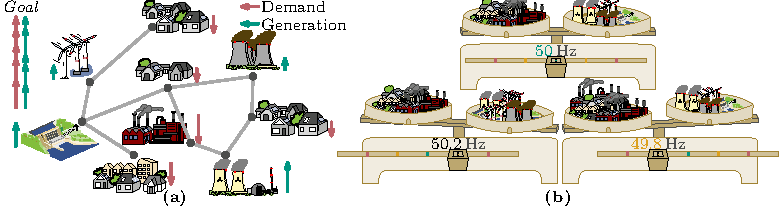
\includegraphics{foundations/figures/feasibility-problem.pdf}
    % 
    \caption[Simple description of the feasibility problem.]{The aim of the
    feasibility problem is to check whether the generation and demand are
    equivalent. This idea is shown by the two schematic sketches in (a) and (b).
    (a) gives a rough idea of the feasibility problem in terms of the power
    grid's generation and demand, (b) represents the same idea in the context of
    the (nominal) frequency of~\SI{50}{\glssymbol{hertz}} (top scale). The
    latter shows that any imbalance leads to a frequency that deviates from the
    nominal frequency in either way. If the generation is to high the frequency
    increases (bottom left scale). However, if the consumption is to high the
    frequency drops (bottom right scale).
    % 
    }%
    % 
    \label{ch:foundations:fig:feasibility-problem}
    % 
\end{figure}

Recall that the subproblem of any power grid analysis and thus, every placement
problem, is~\gls{feas}, \ie, whether there is a feasible power flow
for a given generation and demand. This problem is solved to check the
reliability of the power grid, to do short- and long-term planning (\ie,
placement problems; see~\cref{ch:switching,ch:facts}) and to solve other power
grid related problems. In this section, we will give an overview of the
different basic models, complexities, and relaxations.
% 
%%%%%%%%%%%%%%%%%%%%%%%%%%%%%%%%%%%%%%%%%%%%%%%%%%%%%%%%%%%%%%%%%%%%%%%%%%%%%%%%
\subsection{Alternating Current Power Flow Model}
\label{ch:foundations:sec:power-flow-analyses:subsec:AC-Model}
%%%%%%%%%%%%%%%%%%%%%%%%%%%%%%%%%%%%%%%%%%%%%%%%%%%%%%%%%%%%%%%%%%%%%%%%%%%%%%%%
% 
The~\acrlong{ac} (\gls{ac}) power flow models are the standard models for the
power flow analyses. Models are a description of the real-world that make
certain assumptions such that we have to explain why the models that we use are
reasonable for the problems that we tackle in this thesis. In this section, we
briefly introduce and describe~\gls{ac}~\gls{feas} that describes the power flow
in an~\gls{ac} power grid. We start with the dynamic~\gls{ac} model that is a
very precise model, but also a very complex model. Note that most placement
problems in power grids are long-term decisions. For long-term scenarios, it is
reasonable---since the power grid converges towards a stable state---to make an
assumption such that the~\gls{ac} model becomes time-independent
(see~\cref{ch:foundations:sec:power-flow-analyses:eq:complex-power-injection-resolution}).
The time-independent model is called~\emph{static}~\gls{ac} model. Using
different transformations, we derive different formulations
for~\gls{ac}~\gls{feas} shifting the non-convex and non-linear formulas in
different parts of the system of equations (see~\cref{tbl:ac-model-comparison}).
For problems that are long-term decisions these models are good approximations.
However, \gls{ac}~\gls{feas} is already~\NP-hard on star-shaped
networks~\parencite{Leh16}. In this work, we focus on high-voltage power grids
only, so we can make some assumption that lead to a linearization of~\gls{ac}
models. The linearization is called~\gls{dc}~\gls{feas}, which will be described
in the next section 
(\cref{ch:foundations:sec:power-flow-analyses:subsec:Lin-DC-Model}).

Typically, the theoretical structure of an~\gls{ac} model represents a
subproblem of different power grid problems that have to be solved within
different time ranges depending on the purpose. For instance, for power grid
planning (\ie, \acrlong{tnep}; in short~\gls{tnep}) the model has to be solved
every year~\parencite{Cai12}, whereas for day-ahead markets the particular model
has to be solved every day~\parencite{Cai12}. For the~\gls{ac} model there are
no known fast and robust solution techniques~\parencite{Cai12}, which is due to
the solver technologies not being able to guarantee global optimality since they
get stuck in local optima~\parencite[p.391;Chapter 18]{Fou96}.
% 
\begin{figure}[t!]
    % 
    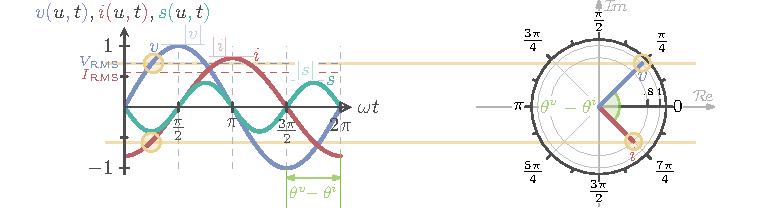
\includegraphics[page=1]{foundations/figures/ac-voltage-vs-current-angles.pdf}
    % 
    \caption[The relationship between voltage and current.]{
        The left side of the figure presents
        \textcolor{VOLTAGE}{voltage~$\textcolor{VOLTAGE}{\glssymbol{voltage}(
        \textcolor{TIMESTAMP}{\vertexa},\textcolor{TIMESTAMP}{\glssymbol{timestamp}})}$},
        \textcolor{CURRENT}
        {current~$\glssymbol{current}(\textcolor{TIMESTAMP}{\vertexa},
        \textcolor{TIMESTAMP}{\glssymbol{timestamp}})$},
        and~\textcolor{COMPLEXPOWER}{total instantaneous electric
        power}~$\textcolor{COMPLEXPOWER}{\glssymbol{complexpower}(\textcolor{TIMESTAMP}{\vertexa},\textcolor{TIMESTAMP}
        {\glssymbol{timestamp}})}$ in terms of trigonometric function for
        timestamp~$\textcolor{TIMESTAMP}{\glssymbol{timestamp}}\in\reals$ and
        vertex~$ \textcolor{TIMESTAMP} {\vertexa}\in\glssymbol{vertices}$. The
        Argand diagram is shown on the right side of the figure, where
        \textcolor{VOLTAGE}{voltage~$\glssymbol{voltage}(\textcolor{TIMESTAMP}{\vertexa},
        \textcolor{TIMESTAMP}{\glssymbol{timestamp}})$} and \textcolor{CURRENT}
        {current~$\glssymbol{current}(\textcolor{TIMESTAMP}{\vertexa},
        \textcolor{TIMESTAMP}{\glssymbol{timestamp}})$} are described by polar
        coordinates.
        % 
        The \textcolor{CURRENT}{current~$\glssymbol{current}(\textcolor{TIMESTAMP}{\vertexa},
        \textcolor{TIMESTAMP}{\glssymbol{timestamp}})$} is shifted
        by~\textcolor{POWERANGLE}{$\nicefrac{\gls{pi}}{2}$} to the right of
        \textcolor{VOLTAGE}{voltage~$\glssymbol{voltage}(\textcolor{TIMESTAMP}{\vertexa},
        \textcolor{TIMESTAMP}{\glssymbol{timestamp}})$} (\ie, voltage acts as
        reference point). The shift between voltage~$\glssymbol{voltage}(\textcolor{TIMESTAMP}{\vertexa},
        \textcolor{TIMESTAMP}{\glssymbol{timestamp}})$ and
        current~$\glssymbol{current}(\textcolor{TIMESTAMP}{\vertexa},
        \textcolor{TIMESTAMP}{\glssymbol{timestamp}})$ by~\textcolor{POWERANGLE}{$
        \glssymbol{voltageangle}-\glssymbol{currentangle}$}
        is also called~\textcolor{POWERANGLE}{power angle}. In the right diagram
        at timestamp~$\textcolor{TIMESTAMP}{\glssymbol{timestamp}} = 0$ the
        \textcolor{VOLTAGE}{voltage
        vector~$\glssymbol{voltage}(\textcolor{TIMESTAMP}{\vertexa},
        \textcolor{TIMESTAMP}{\glssymbol{timestamp}})$} completes a full cycle
        (\ie, a time period), whereas the \textcolor{CURRENT}{current
        vector~$\glssymbol{current}(\textcolor{TIMESTAMP}{\vertexa},
        \textcolor{TIMESTAMP}{\glssymbol{timestamp}})$} is on the negative
        imaginary axis and thus, lags behind the \textcolor{VOLTAGE}{voltage
        vector~$\glssymbol{voltage}(\textcolor{TIMESTAMP}{\vertexa},
        \textcolor{TIMESTAMP}{\glssymbol{timestamp}})$}
        by~\textcolor{POWERANGLE}{$\nicefrac{\gls{pi}}{2}$}. An inductive load
        could be a cause of that particular shift, since the
        \textcolor{VOLTAGE}{voltage~$\glssymbol{voltage}(\textcolor{TIMESTAMP}{\vertexa},
        \textcolor{TIMESTAMP}{\glssymbol{timestamp}})$} leads the
        \textcolor{CURRENT}{current~$\glssymbol{current}(\textcolor{TIMESTAMP}{\vertexa},
        \textcolor{TIMESTAMP}{\glssymbol{timestamp}})$}. The product of
        \textcolor{VOLTAGE}{voltage~$\glssymbol{voltage}(\textcolor{TIMESTAMP}{\vertexa},\textcolor{TIMESTAMP}{\glssymbol{timestamp}})$}
        and
        \textcolor{CURRENT}{current~$\glssymbol{current}(\textcolor{TIMESTAMP}{\vertexa},\textcolor{TIMESTAMP}{\glssymbol{timestamp}})$}
        is equivalent to the \textcolor{COMPLEXPOWER}{total instantaneous
        electric power}~$\textcolor{COMPLEXPOWER}{\glssymbol{complexpower}(
        \textcolor{TIMESTAMP}{\vertexa},\textcolor{TIMESTAMP}
        {\glssymbol{timestamp}})}$. Note that the magnitude of the
        total instantaneous
        electric power corresponds to the product of the~\acrlong{rms}
        (\gls{rms}) of the \textcolor{VOLTAGE}{voltage
        magnitude~$\fmagnitude{\glssymbol{voltage}(\textcolor{TIMESTAMP}{\vertexa})}$}
        denoted
        by~\textcolor{VOLTAGE}{\glssymbol{voltagerms}(\textcolor{TIMESTAMP}{\vertexa})}
        and the \textcolor{CURRENT}{current
        magnitude~$\fmagnitude{\glssymbol{current}(\textcolor{TIMESTAMP}{\vertexa})}$}
        denoted by~\textcolor{CURRENT}{
        \glssymbol{currentrms}(\textcolor{TIMESTAMP}{\vertexa})}. The derivation of this figure can be
        found
        in~\cref{ch:appendix:sec:fundamentals:sinusoid-plot-derivation}.
    %
    }%
    % 
    \label{ch:foundations:fig:AC-voltage-current-angle-difference}
    % 
\end{figure}
% 
\paragraph{Dynamic AC Model}
% 
The~\gls{ac} power flow in general consists of functions representing complex
current
injection~$\glssymbol{current}\colon\glssymbol{vertices}\times\reals\to\complexes$
and complex voltages injection~$\glssymbol{voltage}\colon
\glssymbol{vertices}\times\reals\to\complexes$ at a
vertex~$\vertexa\in\glssymbol{vertices}$ and timestamp~$\glssymbol{timestamp}\in\reals$ that are
sinusoid functions with amplitude~$\fmagnitude{\glssymbol{current}}$ and~$
\fmagnitude{\glssymbol{voltage}}$, respectively, angular
frequency~$\glssymbol{angularfrequency}\coloneqq\nicefrac{d\aangle}
{d\glssymbol{timestamp}}$ (\ie, \glssymbol{frequency} being the frequency; \eg,
\SI{50}{\glssymbol{hertz}} or~\SI{60}{\glssymbol{hertz}}), initial phases for
voltage and
current~$\glssymbol{voltageangle}\colon\glssymbol{vertices}\to\reals$
and~$\glssymbol{currentangle}\colon\glssymbol{vertices}\to\reals$, respectively,
and complex coefficients. 

The electrical power is defined by complex current~$\glssymbol{current}$ and
complex voltage~$\glssymbol{voltage}$ such that the complex
power~$\glssymbol{complexpower}(\vertexa,\glssymbol{timestamp})$ is defined
by~\cref{ch:foundations:sec:power-flow-analyses:eq:complex-power-vi}. 
% 
\begin{align}
    % 
    \glssymbol{complexpower}(\vertexa,\glssymbol{timestamp}) 
    % 
    &\coloneqq
    % 
    \glssymbol{voltage}(\vertexa,\glssymbol{timestamp})
    \cdot
    \conjugate{\glssymbol{current}(\vertexa,\glssymbol{timestamp})}
    &\qquad
    \forall
    \vertexa\in\glssymbol{vertices},
    \glssymbol{timestamp}\in\reals, 
    % 
    \label{ch:foundations:sec:power-flow-analyses:eq:complex-power-vi}
    % 
\end{align}
% 
where~$\conjugate{\glssymbol{current}(\vertexa,\glssymbol{timestamp})}$ is the complex
conjugate of the current. Since we use the complex conjugate of the current, we
get the relationship between voltage and current (see
also~\cref{ch:foundations:fig:AC-voltage-current-angle-difference}) that is the
difference between the voltage angle~\glssymbol{voltageangle} and the current
angle~\glssymbol{currentangle} meaning~$\glssymbol{voltageangle}-
\glssymbol{currentangle}$
(see~\cref{ch:foundations:sec:power-flow-analyses:eq:complex-power-injection-resolution}).
The latter difference is also called~\emph{power angle}. Thus, the function that
represents the complex power injection is defined
by~$\glssymbol{complexpower}\colon\glssymbol{vertices}\times\reals\to\complexes$.
% 
The real and imaginary part of a complex number~$z\in\complexes$ is denoted by~$
\real{z}$ and~$\imaginary{z}$, respectively. The voltage magnitude~$
\fmagnitude{\glssymbol{voltage}(\vertexa)}$
(\cref{ch:foundations:sec:power-flow-analyses:eq:voltage-magnitude}) represents
the wave crest (see left side
of~\cref{ch:foundations:fig:AC-voltage-current-angle-difference}) at
vertex~$\vertexa\in\glssymbol{vertices}$.
%
\begin{align}
    \fmagnitude{\glssymbol{voltage}(\vertexa)}
    &=
    \sqrt{\real{\glssymbol{voltage}(\vertexa,\glssymbol{timestamp})}^2 
    +
    \imaginary{\glssymbol{voltage}(\vertexa,\glssymbol{timestamp})}^2}.
    % 
    \label{ch:foundations:sec:power-flow-analyses:eq:voltage-magnitude}
\end{align}
% 
The current magnitude~$\fmagnitude{\glssymbol{current}(\vertexa)}$ is defined
accordingly
to~\cref{ch:foundations:sec:power-flow-analyses:eq:voltage-magnitude}. The
voltage and current magnitude are time independent,
since~\cref{ch:foundations:sec:power-flow-analyses:eq:voltage-magnitude} can be
written using trigonometric function~$\fmagnitude{\glssymbol{voltage}
(\vertexa)}\cdot$ $\sqrt{\cos^2
(\glssymbol{voltageangle}(\vertexa)+\glssymbol{angularfrequency}\glssymbol{timestamp})
+
\sin^2(\glssymbol{voltageangle}(\vertexa)+
\glssymbol{angularfrequency}\glssymbol{timestamp})}$, where the Pythagorean identity~$\sqrt{\cos^2
(\glssymbol{voltageangle}(\vertexa)+\glssymbol{angularfrequency}\glssymbol{timestamp}) +
\sin^2(\glssymbol{voltageangle}(\vertexa)+
\glssymbol{angularfrequency}\glssymbol{timestamp})} = 1$ follows from the complex plane
representation. 

% 
The idea behind this is that the assumption of time-invariance results in an
unchanging (\ie, constant) wave crest over time.
% 
If we assume that all functions are \emph{time-invariant}---having the same
behavior for the same input at any timestamp, \ie, the angular
frequency~$\nicefrac{d\aangle}{d\glssymbol{timestamp}} = \glssymbol{twopi}
\glssymbol{frequency}$ is constant---then we call them current and voltage
phasors. This allows us to use the phasor transform of Charles Proteus
Steinmetz~\parencite{Yan08,Rob12} such that we can use simple algebraic
equations on the phasors instead of differential equations of the sinusoid
signals. Note that the assumption of time-invariance might be acceptable for
some power flow analyses and planning problems. However, for smaller periods of
time such as the influence of switching processes on the grid stability this
assumption might not be suitable anymore. However, then we get into the range of
dynamic analyses~\parencite{Str18,Roh12,Tim14,Tim18}.

% 
We get the trigonometric relationship depicted
in~\cref{ch:foundations:sec:power-flow-analyses:eq:complex-power-injection-resolution}.
The derivation can be found
in~\cref{app:foundations:sec:power-flow-analyses:eq:complex-power-injection-resolution}.
%
\begin{subequations}
    \wormhole{bit:ch:foundations:sec:power-flow-analyses:eq:complex-power-injection-resolution} 
    \small
\begin{alignat}{2}
    \glssymbol{complexpower}(\vertexa,\timestamp) 
    &=
        \glssymbol{voltage}(\vertexa,\timestamp)
        \hspace{3.0cm}\cdot
        \conjugate{\glssymbol{current}(\vertexa,\timestamp)}
    \\
    &\begin{aligned}
        &=
        \hphantom{-\imgPart\cdot\big(}
        {\underbrace{
            \begin{aligned}
                \real{\glssymbol{voltage}(\vertexa,\timestamp)}
                \cdot
                \real{\glssymbol{current}(\vertexa,\timestamp)}
                +
                \imaginary{\glssymbol{voltage}(\vertexa,\timestamp)}
                \cdot
                \imaginary{\glssymbol{current}(\vertexa,\timestamp)}
            \end{aligned}
        }_{\eqqcolon\glssymbol{realpower}(\vertexa)}}%
        \\
        &\,\,\,\,-
        \imgPart\cdot
        {\underbrace{
            \begin{aligned}
                \big(
                    \real{\glssymbol{voltage}(\vertexa,\timestamp)}
                    \cdot
                    \imaginary{\glssymbol{current}(\vertexa,\timestamp)}
                    -
                    \imaginary{\glssymbol{voltage}(\vertexa,\timestamp)}
                    \cdot
                    \real{\glssymbol{current}(\vertexa,\timestamp)}
                \big)
            \end{aligned}
        }_{\eqqcolon\glssymbol{reactivepower}(\vertexa)}}%
    \end{aligned}%
    % 
    \label{ch:foundations:sec:power-flow-analyses:eq:complex-power:iv:rectangular}
    \\
    &=
        % \frac{1}{2}
        \fmagnitude{\glssymbol{voltage}(\vertexa)}
        \fmagnitude{\glssymbol{current}(\vertexa)} 
        \Big(
            \fcos{
                \glssymbol{voltageangle}(\vertexa) 
                + \angularfrequency\timestamp 
                - \glssymbol{currentangle}(\vertexa) 
                - \angularfrequency\timestamp
                } 
            +
            \imgPart\cdot
                \fsin{
                    \glssymbol{voltageangle}(\vertexa)  
                    + \angularfrequency\timestamp 
                    - \glssymbol{currentangle}(\vertexa)  
                    - \angularfrequency\timestamp
                    }
        \Big)
        \label{ch:foundations:sec:power-flow-analyses:eq:complex-power:iv:polar}
    \\
    &=
        \underbrace{
            % \frac{1}{2}
            \fmagnitude{\glssymbol{voltage}(\vertexa)}
            \fmagnitude{\glssymbol{current}(\vertexa)} 
            \fcos{\glssymbol{voltageangle}(\vertexa)
            - \glssymbol{currentangle}(\vertexa)} 
        }_{=\glssymbol{realpower}(\vertexa)}
        \hspace{16.7mm}+\hspace{0.5mm}
        \imgPart\cdot
        \underbrace{
            % \frac{1}{2}
            \fmagnitude{\glssymbol{voltage}(\vertexa)}
            \fmagnitude{\glssymbol{current}(\vertexa)}
            \fsin{\glssymbol{voltageangle}(\vertexa) - \glssymbol{currentangle}(\vertexa) } 
        }_{=\glssymbol{reactivepower}(\vertexa)}
        \label{ch:foundations:sec:power-flow-analyses:eq:complex-power:iv:polar:p:q}
    % 
\end{alignat}
    \label{ch:foundations:sec:power-flow-analyses:eq:complex-power-injection-resolution}
\end{subequations}
% 
Note that we have to use the~\acrlong{rms} (\gls{rms}) values
in~\cref{ch:foundations:sec:power-flow-analyses:eq:complex-power:iv:polar},
since $\fmagnitude{\glssymbol{voltage}(\vertexa)}\fmagnitude{\glssymbol{current}
(\vertexa)}$ would lead in a magnitude that is twice as high as of~$
\glssymbol{voltage}(\vertexa,\glssymbol{timestamp})\cdot\glssymbol{current}
(\vertexa,\glssymbol{timestamp})^\star$, which is graphically illustrated in~\cref{ch:foundations:fig:AC-voltage-current-angle-difference}. 
% 
To illustrate the time-varying power
in~\cref{ch:foundations:fig:AC-voltage-current-angle-difference}, we use the
concept of instantaneous electric power
(see~\cref{ch:appendix:sec:fundamentals:sinusoid-plot-derivation}), since the
complex power becomes time-independent
in~\cref{ch:foundations:sec:power-flow-analyses:eq:complex-power-injection-resolution}
and thus, constant. To illustrate the signals of the complex power a common way
is to use the real part of a signal (in our case the real part of the
current~\glssymbol{current} and voltage~\glssymbol{voltage},
see~\cref{ch:appendix:sec:fundamentals:sinusoid-plot-derivation} for more
details).

The penultimate step
in~\cref{ch:foundations:sec:power-flow-analyses:eq:complex-power-injection-resolution}
follows from the trigonometric addition and product formulas. In the last step,
the complex power equation becomes independent from time~\glssymbol{timestamp} and angle
frequency~\glssymbol{angularfrequency}. The intuition behind this is that in an
ideal~\gls{ac} network we start with the initial phase
angles~\glssymbol{voltageangle} and~\glssymbol{currentangle}, but the angular
frequency stays constant
meaning~$\glssymbol{angularfrequency}\coloneqq\nicefrac{d\aangle}{d\glssymbol{timestamp}} =
\glssymbol{twopi}\glssymbol{frequency}$. Thus, the rotation velocity is the same
for
both current and voltage. This simplifies the system such that it only depends
on the initial phases
(see~\cref{ch:foundations:fig:AC-voltage-current-angle-difference}) and leads
to a static analysis by using the resulting time-independent models that are
also called static models.
% 
\begin{figure}[t!]
    % 
    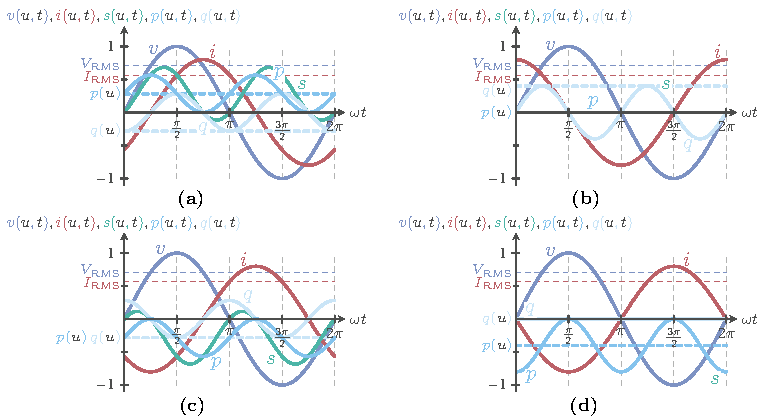
\includegraphics[page=1]{foundations/figures/ac-with-different-angles.pdf}
    % 
    \caption[Time varying~\gls{ac} sinusoid curves with different voltage angle
    differences.]{%
    % 
    The time varying sinusoid curves of
    \textcolor{VOLTAGE}{voltage~$\glssymbol{voltage}(\textcolor{TIMESTAMP}
    {\vertexa},\textcolor{TIMESTAMP}{\glssymbol{timestamp}})$}
    with
    magnitude~$\textcolor{VOLTAGE}{\fmagnitude{\glssymbol{voltage}(\textcolor{TIMESTAMP}
    {\vertexa}) }} = 1$ and effective
    value~$\textcolor{VOLTAGE}{\glssymbol{voltagerms}(\textcolor{TIMESTAMP}
    {\vertexa})} =
    \nicefrac{1}{\sqrt{2}}$, \textcolor{CURRENT}{current~$\glssymbol{current}(\textcolor{TIMESTAMP}
    {\vertexa},\textcolor{TIMESTAMP}{\glssymbol{timestamp}})$}
    with magnitude~$
    \textcolor{CURRENT}{\fmagnitude{\glssymbol{current}(\textcolor{TIMESTAMP}
    {\vertexa})}} = 0.8$ and effective
    value~$\textcolor{CURRENT}{\glssymbol{currentrms}(\textcolor{TIMESTAMP}
    {\vertexa})} =
    \nicefrac{0.8}{\sqrt{2}}$, \textcolor{COMPLEXPOWER}{total instantaneous
    electric
    power~$\glssymbol{complexpower}(\textcolor{TIMESTAMP}
    {\vertexa},\textcolor{TIMESTAMP}{\glssymbol{timestamp}})$}, its
    \textcolor{REALPOWER} {real
    part~$\glssymbol{realpower}(\textcolor{TIMESTAMP}{\vertexa},\textcolor{TIMESTAMP}{\glssymbol{timestamp}})$},
    and its \textcolor{REACTIVEPOWER}{imaginary part~$\glssymbol{reactivepower}(
    \textcolor{TIMESTAMP}{\vertexa},\textcolor{TIMESTAMP}{\glssymbol{timestamp}})$}
    are given for different voltage angle
    differences~\glssymbol{voltageangledifference}. The voltage angle
    differences are (a)~$\glssymbol{voltageangledifference} =
    \nicefrac{\gls{pi}}{4}$, (b)~$
    \glssymbol{voltageangledifference} = -\nicefrac{\gls{pi}}{2}$, (c)~$
    \glssymbol{voltageangledifference} = \nicefrac{3\gls{pi}}{4}$, and (d)~$
    \glssymbol{voltageangledifference} = \gls{pi}$. The 
    \textcolor{COMPLEXPOWER}{total instantaneous electric
    power~$\glssymbol{complexpower}(\textcolor{TIMESTAMP}
    {\vertexa},\textcolor{TIMESTAMP}{\glssymbol{timestamp}})$} is the sum of the
    \textcolor{REALPOWER}{real part~$\glssymbol{realpower}(\textcolor{TIMESTAMP}
    {\vertexa},\textcolor{TIMESTAMP}{\glssymbol{timestamp}})$} and the
    \textcolor{REACTIVEPOWER}{imaginary part~$\glssymbol{reactivepower}(
    \textcolor{TIMESTAMP} {\vertexa},\textcolor{TIMESTAMP}
    {\glssymbol{timestamp}})$} of the power. The same behavior is shown for
    the~\textcolor{COMPLEXPOWER}{complex
    power~$\glssymbol{complexpower}(\textcolor{TIMESTAMP}{\vertexa})$} and
    its~\textcolor{REALPOWER}{real power~$\glssymbol{realpower}(
    \textcolor{TIMESTAMP}{\vertexa})$} and~\textcolor{REACTIVEPOWER}{reactive
    power~$\glssymbol{reactivepower}(\textcolor{TIMESTAMP}{\vertexa})$}. (a)~A
    stable case is represented that is an operation of
    \textcolor{CURRENT}{current~\glssymbol{current}} and
    \textcolor{VOLTAGE}{voltage~\glssymbol{voltage}} within an angle shift
    of~$[-\nicefrac{\gls{pi}}{2};\nicefrac{\gls{pi}}{2}]$. (b)~One of the
    stability borders is~$-\nicefrac{\gls{pi}}{2}$, where the real part of the
    \textcolor{COMPLEXPOWER}{total instantaneous electric
    power~$\glssymbol{complexpower}(\textcolor{TIMESTAMP}
    {\vertexa},\textcolor{TIMESTAMP}{\glssymbol{timestamp}})$} is zero over
    \textcolor{TIMESTAMP}{time~$\glssymbol{timestamp}$}. (c)~With a voltage
    angle difference of~$\nicefrac{3\gls{pi}}{4}$ the power is within the
    instable section. All power curves are in the negative part. (d)~The
    \textcolor{CURRENT}{current~$\glssymbol{current}(\textcolor{TIMESTAMP}
    {\vertexa},\textcolor{TIMESTAMP}{\glssymbol{timestamp}})$} and
    \textcolor{VOLTAGE}{voltage~$\glssymbol{voltage}(\textcolor{TIMESTAMP}
    {\vertexa},\textcolor{TIMESTAMP}{\glssymbol{timestamp}})$} waves are in a
    state, where the waves cancel each other out. The reactive part of the total
    instantaneous electric power curve is zero and the real power part is
    negative. The derivation of this figure can be found
    in~\cref{ch:appendix:sec:fundamentals:sinusoid-plot-derivation}.
    % 
    }%
    % 
    \label{ch:foundations:fig:ac-with-different-angles}
    % 
\end{figure}
% Though the idealization of the angular frequency to a constant is for certain
% scenarios---as mentioned above---not suitable. 
\paragraph{Static AC Models}
% 
For general cases a common way to analyze power grids is to use a constant
angular frequency and analyze steady-state power grids that have one
fixed timestamp
per analysis. This will be our main focus in this work. However, the
idealization of the angular frequency to a constant is not suitable for certain
scenarios, as mentioned above. For this work it means that all previous
functions~$\mathbb{f}$ become time-independent~$\mathbb{f}\colon\mathbb{S}\to
\mathbb{F}$, where~$\mathbb{F}$ is a field and~$\mathbb{S}$ is the set we do the
mapping from such that for example the voltage function
becomes~$\glssymbol{voltage}\colon\glssymbol{vertices}\to\reals$.

\cref{ch:foundations:sec:power-flow-analyses:eq:complex-power:iv:polar} can be
rewritten to~$\glssymbol{complexpower}(\vertexa)\coloneqq\fmagnitude{\glssymbol{voltage}
(\vertexa)}\fmagnitude{\glssymbol{current}(\vertexa)}
e^{\imgPart\cdot(\glssymbol{voltageangle}(\vertexa) -
\glssymbol{currentangle}(\vertexa))}$ using Euler's formula. The
functions~$\glssymbol{realpower}\colon\glssymbol{vertices}\to\reals$
and~$\glssymbol{reactivepower}\colon\glssymbol{vertices}\to\reals$ represent the
\emph{real} and the \emph{reactive power}, respectively. This equation shows
very clearly the current angle~\glssymbol{currentangle} and voltage
angle~\glssymbol{voltageangle} that describe the real and reactive power on each
edge. \cref{ch:foundations:fig:AC-voltage-current-angle-difference} shows the
relationship of current~\glssymbol{current} and voltage~\glssymbol{voltage}. The
difference between voltage and current is the phase angle difference. The more
we increase the phase angle difference (\eg,
see~\cref{ch:foundations:fig:ac-with-different-angles} on
Page~\pageref{ch:foundations:fig:ac-with-different-angles}) between current and
voltage the smaller the real power gets until a certain point
(see~\cref{ch:foundations:fig:ac-with-different-angles}\screen{b}), where the
real power becomes zero. The case, where the wave crests of voltage and current
cancel each other out is shown
in~\cref{ch:foundations:fig:ac-with-different-angles}\screen{d}. Note that the
reactive power (also known as phantom power) increases while the real power
decreases, since current and voltage amplitudes do not decrease. The latter
basically describes the \emph{principle of conservation of energy}. The
described relationship between voltage, current, and power can be used to
maintain the voltage stability by changing real power demands. A decrease in
real power demand can be maintained by an increase in reactive power by changing
the phase angle difference between voltage and current. This mechanism helps to
maintain voltage on a certain level.

The complex power injection can be written in terms of real and reactive power
injection that represent decoupled parts
(see~\cref{ch:foundations:sec:power-flow-analyses:eq:complex-power-injection}
and its derivation
in~\cref{ch:foundations:sec:power-flow-analyses:eq:complex-power-injection-resolution}).
%   
\begin{align}
    \glssymbol{complexpower}(\vertexa) 
    % 
    = \real{\glssymbol{complexpower}(\vertexa)} 
    + \imgPart \cdot \imaginary{\glssymbol{complexpower}(\vertexa)} 
    % 
    = \glssymbol{realpower}(\vertexa) 
    + \imgPart \cdot \glssymbol{reactivepower}(\vertexa)
    % 
    \qquad
    \forall \vertexa\in\glssymbol{vertices}.
    % 
    \label{ch:foundations:sec:power-flow-analyses:eq:complex-power-injection}
\end{align}
% 
This relationship is shown
in~\cref{ch:foundations:fig:ac-with-different-angles}, where the total
instantaneous power~$\glssymbol{complexpower}(\vertexa,\glssymbol{timestamp})$
(respectively complex power~$\glssymbol{complexpower}(\vertexa)$) is the sum of
the real part~$\glssymbol{realpower} (\vertexa,\glssymbol{timestamp})$ and
imaginary part~$\glssymbol{reactivepower}(\vertexa,\glssymbol{timestamp})$ of
the power (respectively real power~$\glssymbol{realpower}(\vertexa)$ and
reactive power~$\glssymbol{reactivepower}(\vertexa)$). The total instantaneous
power curve~$\glssymbol{complexpower}(\vertexa,\glssymbol{timestamp})$
(respectively complex power~$\glssymbol{complexpower}(\vertexa)$) has the same
magnitude independent of the power angle. The latter emphasize the principle of
conservation of energy.

The real power~\glssymbol{realpower} is the power that is actually doing work
such as heating. However, reactive power is seldom consumed by consumers.
Exceptions are motors, generators and transformers that use a magnetic field
(inductive components) of industrial consumers that need reactive power. In
general reactive power is used to maintain the voltage stability. Increasing the
amount of reactive power increases the voltage that has to be kept in a certain
range. So reactive power is necessary for the power grid to have a more
efficient real power flow. The stability of the power grid is maintained by a
balance between real and reactive power and the latter depends highly on the
consumed real power.

We usually do a vertex-based analysis meaning that flows are usually modeled by
disturbance and injection at a vertex. We introduced for each vertex eight
variables denoted by~$\glssymbol{realpowergeneration}(\vertexa)$,
$\glssymbol{reactivepowergeneration}(\vertexa)$, $\glssymbol{realpowerdemand}
(\vertexa)$, $\glssymbol{reactivepowerdemand}(\vertexa)$,
$\glssymbol{voltage}(\vertexa)$, $\glssymbol{current}(\vertexa)$,
$\glssymbol{voltageangle}(\vertexa)$, and~$\glssymbol{currentangle}(\vertexa)$
for all~$\vertexa\in\glssymbol{vertices}$. However, we can always reformulate
current~$\glssymbol{current}$ and current angles~$\glssymbol{currentangle}$ in
terms of voltage~$\glssymbol{voltage}$ and voltage
angle~$\glssymbol{voltageangle}$ using Ohm's law and thus, we have just six
variables. We will see later that depending on the vertex type
(see~\cref{ch:foundations:tbl:load-flow-bus-specification}) or on the problem
some variables are given and thus, fixed to a certain value.

Up to now, we just looked at the power~\emph{injections} and not the
power~\emph{flows}. However, the complex, real, and reactive power flow, as well
as the complex current flow are defined by the
functions~$\glssymbol{complexpower}\colon\glssymbol{edges}\to\complexes$ (in
Volt Ampere; short~\SI{}{\gls{voltampere}}), $\glssymbol{realpower}\colon
\glssymbol{edges}\to\reals$ (in~\SI{}{\gls{watt}}),
$\glssymbol{reactivepower}\colon\glssymbol{edges}\to\reals$ (in Volt Ampere
Reactive; short~\SI{}{\gls{var}}), and~$\glssymbol{current}\colon
\glssymbol{edges}\to\complexes$ (in Ampere; short~\SI{}{\gls{ampere}}),
respectively. We distinguish between the injection at the source and sink vertex
of each edge, since there are power losses at each electrical element. 
% Depending
% on the problem statement, the above functions are usually unknown.
% 
\begin{figure}
    % 
    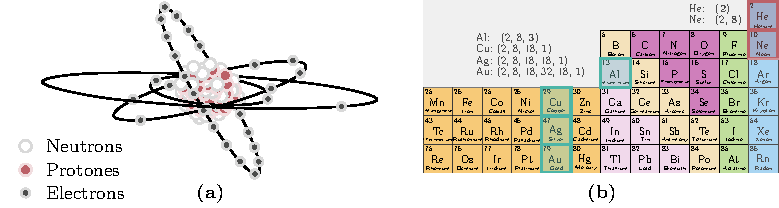
\includegraphics{foundations/figures/admittance.pdf}
    % 
    \caption[Relationship between conductivity and the material's atomic
    structure.]{Both (a) and (b) represent the atomic structure of one element
    and of multiple elements, respectively. The conductivity is dependent on the
    outermost shell denoted by valence shell. (a) The copper-$29$ isotope that
    has fully filled electron shells, but the valence shell (outermost shell).
    The valence shell has just one electron that is highly reactive. (b) Part of
    the description of the atomic structure of elements. The green marked
    elements represent common conductors and the red marked elements are strong
    insulators that are all in the last column.%
    }%
    % 
    \label{ch:foundations:sec:power-flow-analyses:fig:atomic-structure}
    % 
\end{figure}
% 
%%%%%%%%%%%%%%%%%%%%%%%%%%%%%%%%%%%%%%%%%%%%%%%%%%%%%%%%%%%%%%%%%%%%%%%%%%%%%%%%
\paragraph{Network Parameters}
\label{ch:foundations:network-parameters}
%%%%%%%%%%%%%%%%%%%%%%%%%%%%%%%%%%%%%%%%%%%%%%%%%%%%%%%%%%%%%%%%%%%%%%%%%%%%%%%%
% 
% 
The~\gls{ac}~network~\acnetworktuple is defined by the topological structure
that is given by the graph~$\glssymbol{graph} = (\glssymbol{vertices},
\glssymbol{edges})$,
the set~$\glssymbol{generators}\subseteq\glssymbol{vertices}$ of generators, the
set~$\glssymbol{consumers}\subseteq\glssymbol{vertices}$ of consumers,
% 
the resistance function~$\glssymbol{resistance}\colon
\glssymbol{undirectededges}\to\posreals\cup
\{\infty\}$,
% 
the reactance
function~$\glssymbol{reactance}\colon\glssymbol{undirectededges}\to\posreals\cup
\{\infty\}$,
% 
the susceptance
function~$\glssymbol{susceptance}\colon\glssymbol{undirectededges}\to\reals$~(\cref{ch:foundations:sec:power-flow-analyses:eq:susceptance}),
% 
the conductance function~$\glssymbol{conductance}\colon
\glssymbol{undirectededges}\to\reals$~(\cref{ch:foundations:sec:power-flow-analyses:eq:conductance}),
% 
the admittance
function~$\glssymbol{admittance}\colon\glssymbol{undirectededges}\to\complexes$~(\cref{ch:foundations:sec:power-flow-analyses:eq:admittance}),
% 
and the apparent power's thermal line limit
function~$\glssymbol{capacity}\colon\glssymbol{undirectededges}\to\reals$, which
can be either~$\glssymbol{currentmax}, \glssymbol{complexpowermax},
\glssymbol{realpowermax}$, or~$\glssymbol{reactivepowermax}$, and combinations
of them. The resistance~\glssymbol{resistance} and the
reactance~\glssymbol{reactance} are measured in Ohm~\gls{ohm}. The
admittance~$\glssymbol{admittance}(\vertexa,\vertexb)$~(\cref{ch:foundations:sec:power-flow-analyses:eq:admittance})
is defined by the
conductance~$\glssymbol{conductance}(\vertexa,\vertexb)$~(\cref{ch:foundations:sec:power-flow-analyses:eq:conductance})
and the
susceptance~$\glssymbol{susceptance}(\vertexa,\vertexb)$~(\cref{ch:foundations:sec:power-flow-analyses:eq:susceptance})
that defines how easy the current is able to flow through an element such as a
transmission line~$\{\vertexa,\vertexb\}\in\glssymbol{undirectededges}$. Note
that all three are measured in Siemens~\gls{siemens}. The conductivity of an
electrical element is mainly influenced by the conductance of the material,
length, and wire gauge. The conductance of the material is mainly influenced by
the atomic structure
(see~\cref{ch:foundations:sec:power-flow-analyses:fig:atomic-structure}).
Elements that have just one electron on the valence shell (\ie, outermost shell)
have a high conductivity such as copper, gold, and silver (Column 11 of the
periodic system;
see~\cref{ch:foundations:sec:power-flow-analyses:fig:atomic-structure}\screen{b}
green markers). However, elements that have a full valence shell are very good
insulators since the conductivity is very low, \eg, helium (last column of the
periodic system;
see~\cref{ch:foundations:sec:power-flow-analyses:fig:atomic-structure} red
markers). The admittance~\glssymbol{admittance},
impedance~\glssymbol{impedance}, conductance~\glssymbol{conductance}, and
susceptance~\glssymbol{susceptance} are defined
in~\crefrange{ch:foundations:sec:power-flow-analyses:eq:admittance}{ch:foundations:sec:power-flow-analyses:eq:susceptance}.
% 
\begin{align}
        \glssymbol{admittance}(\vertexa,\vertexc) 
&\coloneqq 
    \frac{1}{\glssymbol{impedance}(\vertexa,\vertexc)} =
    \glssymbol{conductance}(\vertexa,\vertexc) 
+ 
    \imgPart\cdot\glssymbol{susceptance}(\vertexa,\vertexc)
& \forall \{\vertexa,\vertexc\}\in\glssymbol{undirectededges},
% 
\label{ch:foundations:sec:power-flow-analyses:eq:admittance}
\\
    \glssymbol{impedance}(\vertexa,\vertexc) 
&\hphantom{:}=
    \frac{1}{\glssymbol{admittance}(\vertexa,\vertexc)} 
=
    \glssymbol{resistance}(\vertexa,\vertexc) 
+ 
    \imgPart\cdot\glssymbol{reactance}(\vertexa,\vertexc)
& \forall \{\vertexa,\vertexc\}\in\glssymbol{undirectededges},
% 
\label{ch:foundations:sec:power-flow-analyses:eq:impedance}
\\
    \glssymbol{conductance}(\vertexa,\vertexc) 
&\coloneqq
    \frac{\glssymbol{resistance}(\vertexa,\vertexc)}
    {\glssymbol{resistance}(\vertexa,\vertexc)^2 + \glssymbol{reactance}(\vertexa,\vertexc)^2}
& \forall \{\vertexa,\vertexc\}\in\glssymbol{undirectededges},
% 
\label{ch:foundations:sec:power-flow-analyses:eq:conductance}
\\
    \glssymbol{susceptance}(\vertexa,\vertexc) 
&\coloneqq 
    - \frac{\glssymbol{reactance}(\vertexa,\vertexc)}
    {\glssymbol{resistance}(\vertexa,\vertexc)^2 + \glssymbol{reactance}(\vertexa,\vertexc)^2}
& \forall \{\vertexa,\vertexc\}\in\glssymbol{undirectededges}.
% 
\label{ch:foundations:sec:power-flow-analyses:eq:susceptance}
\end{align}

Note that the admittance matrix~$\mathbf{\admittances}$ is defined by
the self-admittances representing the diagonal entries~$\glssymbol{admittance}
(\vertexa,\vertexa) = \glssymbol{admittance}(\vertexa,0) -
\sum_{\{\vertexa,\vertexc\}\in\glssymbol{undirectededges}}\glssymbol{admittance}
(\vertexa,\vertexc)$, where~$\glssymbol{admittance}(\vertexa,0)$ is the
admittance to ground, and the entries
of~\cref{ch:foundations:sec:power-flow-analyses:eq:admittance} that represent
the entries for the incident edge.
% 
%%%%%%%%%%%%%%%%%%%%%%%%%%%%%%%%%%%%%%%%%%%%%%%%%%%%%%%%%%%%%%%%%%%%%%%%%%%%%%%%
\paragraph{Power Grid Bounds}%
\label{ch:foundations:power-grid-bounds}
%%%%%%%%%%%%%%%%%%%%%%%%%%%%%%%%%%%%%%%%%%%%%%%%%%%%%%%%%%%%%%%%%%%%%%%%%%%%%%%%
% 
There are lower and upper bounds restricting the voltage angle
differences~$\glssymbol{voltageangledifferencemin}$
and~$\glssymbol{voltageangledifferencemax}$, the
voltages~\glssymbol{voltagemin}
and~\glssymbol{voltagemax}, the real power generation~
\glssymbol{realpowergenerationmin},
\glssymbol{realpowergenerationmax}, the reactive power
generation~\glssymbol{reactivepowergenerationmin},
\glssymbol{reactivepowergenerationmax},
the real power demand~\glssymbol{realpowerdemandmin},
\glssymbol{realpowerdemandmax}, and the reactive power
demand~\glssymbol{reactivepowerdemandmin},
\glssymbol{reactivepowerdemandmax}, respectively. The constraint of the voltage
angle difference (\cref{ch:foundations:eq-voltage-angle-difference-constraints})
restricts the power flow on each edge
(\cref{ch:foundations:sec:power-flow-analyses:eq:complex-power-injection-resolution}).
% 
\begin{subequations}
    \begin{alignat}{3}
        \glssymbol{voltageangledifferencemin}(\vertexa,\vertexc)
    &\leq
        \glssymbol{voltageangle}(\vertexa)
        &-&
        \glssymbol{voltageangle}(\vertexc)
    &\leq
        \glssymbol{voltageangledifferencemax}(\vertexa,\vertexc),
    % 
    \label{ch:foundations:sec:power-flow-analyses:eq:network:bounds:delta-voltageangle:polar}
    % 
    \\
    % 
        \glssymbol{voltageangledifferencemin}(\vertexa,\vertexc)
    &\leq
        \arctan
        \left(
            \frac{\imaginary{\glssymbol{voltage}(\vertexa)}}{\real{
            \glssymbol{voltage}(\vertexa)}}
        \right)
        &-&
        \arctan%
        \left(
            \frac{\imaginary{\glssymbol{voltage}(\vertexc)}}{\real{
            \glssymbol{voltage}(\vertexc)}}
        \right)
    &\leq
        \glssymbol{voltageangledifferencemax}(\vertexa,\vertexc),
    % 
    \label{ch:foundations:sec:power-flow-analyses:eq:network:bounds:delta-voltageangle:rectangular}
\end{alignat}
    \label{ch:foundations:eq-voltage-angle-difference-constraints}
\end{subequations}%
% 
for all~$\{\vertexa,\vertexc\}\in\glssymbol{undirectededges}$.
In~\cref{ch:foundations:sec:power-flow-analyses:eq:network:bounds:delta-voltageangle:rectangular},
we use the trigonometric relationship of the real part~$\real{
\glssymbol{voltage}(\vertexa)}$ and imaginary
part~$\imaginary{\glssymbol{voltage}(\vertexa)}$ that is defined by~$
\tan\big(\glssymbol{voltageangle}(\vertexa)\big) 
=
\nicefrac{
    \text{adjacent}
  }{
    \text{opposite}
  } 
= 
\nicefrac{
    \imaginary{\glssymbol{voltage}(\vertexa)}
  }{
    \real{\glssymbol{voltage}(\vertexa)}
  } 
= 
\nicefrac{
    \sin\big(\glssymbol{voltageangle}(\vertexa)\big)
  }{
    \cos\big(\glssymbol{voltageangle}(\vertexa)\big)
  }
$.
% 
The voltage angle difference is often restricted to the interval
of~$[-\nicefrac{\gls{pi}}{2};
\nicefrac{\gls{pi}}{2}]$ for stability reasons
(see~\cref{ch:foundations:fig:ac-with-different-angles} for different voltage
angle differences). If the balance between real power generation and demand
cannot be maintained (\ie, is not zero), then there is an issue in the angle
stability, \ie, the voltage angle difference cannot be maintained within the
stability interval. This in particular means the smaller the angle difference
the more balance between real power generation and demand exists. This is due to
the fact that the reactive power is used to compensate the lack of real power
generation and demand by shifting voltage and current using devices such as 
capacitor banks. \cref{ch:foundations:fig:ac-with-different-angles} explains why
exceeding the~$\nicefrac{\gls{pi}}{2}$ would lead to instabilities in the power
grid. Note that mainly generators are able to influence the voltage, power
curves, and the power angle
(see~\cref{ch:foundations:tbl:load-flow-bus-specification}). Thus, the network
stability is mainly driven by generators (including devices such as capacitor
banks). If the power angle exceeds the stability range the power curves shift
into the negative quadrant and the effective power values are negative, too
(see~\cref{ch:foundations:fig:ac-with-different-angles}\screen{b}--\screen{d}).
However, a power grid has a predefined flow direction and a negative real power
can be interpreted as a \textquote{backward power movement}
(see~\cref{ch:foundations:fig:ac-with-different-angles}\screen{a}).
% 
A rough idea of the latter is given by a simple~\gls{dc} circuit with a 
preinstalled diode. Note that a diode has a predefined direction making the
network nonreciprocal. The predefined direction defines the anode and cathode
for the battery connection. Connecting the battery in the wrong sense would lead
to a diode that does not flash.

In addition, the smaller the shift the less losses and the more stable the power
grid works.
In~\cref{ch:foundations:sec:power-flow-analyses:subsec:AC-vs-DC-Model}, we will
see that the differences are often smaller than~$\nicefrac{\gls{pi}}{6}$.
However, the voltage angle difference~$\glssymbol{voltageangledifference}$ also
correlates with the real power that flows from one vertex to another over the
power grid. The relationship becomes much clearer if we look at the
linearization of the~\gls{ac} model
in~\cref{ch:foundations:sec:power-flow-analyses:subsec:Lin-DC-Model}.

In some literature there is a constraint restricting the voltage
angles~$\glssymbol{voltageangle}(\vertexa)$ for
all~$\vertexa\in\glssymbol{vertices}$ themselves
(see~\cref{ch:foundations:sec:power-flow-analyses:eq:network:bounds:voltageangle}).
% 
\begin{equation}
    % \begin{align}
        \glssymbol{minvoltageangle}(\vertexa)
    \leq
        \glssymbol{voltageangle}(\vertexa)
    \leq
        \glssymbol{maxvoltageangle}(\vertexa)
    \qquad
    \forall
        \vertexa\in\glssymbol{vertices}.
    \label{ch:foundations:sec:power-flow-analyses:eq:network:bounds:voltageangle}
% \end{align}
\end{equation}
% 
The latter restricts the solution space and might exclude feasible solutions,
but does not represent a physical constraint. However, it improves the running
times to solve the feasibility problem and to fulfill assumptions such as the
stability range or later the
Assumption~\ref{ch:foundations:sec:power-flow-analyses:assumption:voltage-angle-difference}
in~\cref{ch:foundations:sec:power-flow-analyses:subsec:Lin-DC-Model}.

The voltage magnitude is bounded by
either~\cref{ch:foundations:sec:power-flow-analyses:eq:network:bounds:voltage-magnitude-min:polar},
or
by~\cref{ch:foundations:sec:power-flow-analyses:eq:network:bounds:voltage-magnitude-min:rectangular}
and~\cref{ch:foundations:sec:power-flow-analyses:eq:network:bounds:voltage-magnitude-max:rectangular}
depending on the formulation that is either polar or rectangular, respectively.
% 
\begin{subequations}
    \begin{alignat}{3}
        \fmagnitude{\glssymbol{voltagemin}(\vertexa)}\hphantom{)^2}
    &\leq
        &\fmagnitude{\glssymbol{voltage}(\vertexa)}
    &\leq&
        \fmagnitude{\glssymbol{voltagemax}(\vertexa)}\hphantom{)^2},
    % 
    \label{ch:foundations:sec:power-flow-analyses:eq:network:bounds:voltage-magnitude-min:polar}
    % 
    \\
        \glssymbol{voltagemin}(\vertexa)^2
    &\leq
        &\,\,\real{\glssymbol{voltage}(\vertexa)}^2
    +
        \imaginary{\glssymbol{voltage}(\vertexa)}^2,&&
    % 
    \label{ch:foundations:sec:power-flow-analyses:eq:network:bounds:voltage-magnitude-min:rectangular}
    % 
    \\
        &&\real{\glssymbol{voltage}(\vertexa)}^2 
    + 
        \imaginary{\glssymbol{voltage}(\vertexa)}^2\hphantom{,}
    &\leq&
        \glssymbol{voltagemax}(\vertexa)^2,
    % 
    \label{ch:foundations:sec:power-flow-analyses:eq:network:bounds:voltage-magnitude-max:rectangular}
\end{alignat}
\end{subequations}
% 
for all vertices~$\vertexa\in\glssymbol{vertices}$. This is mainly motivated by
the power grid elements that work within a certain voltage range. 
% 
% A usual range is~$\pm 5\%$ of the nominal voltage, where 
% 
Most elements perform poorly on the lower voltage end---\eg, inductive motors
over\-\mbox{heat---and} on the upper end the elements can get destroyed. The
thermal line limits can be represented in different ways that mainly depend on
the formulation. If the formulation uses current and
voltage, 
\cref{ch:foundations:sec:power-flow-analyses:eq:network:bounds:current-flow,ch:foundations:sec:power-flow-analyses:eq:network:bounds:current-flow:polar}
are used. Otherwise, if it uses real power, reactive power, and voltage
angles, 
\cref{ch:foundations:sec:power-flow-analyses:eq:network:bounds:complex-power-flow,ch:foundations:sec:power-flow-analyses:eq:network:bounds:complex-power:rectangular}
are used.
% 
\begin{subequations}
    \begin{alignat}{2}
    \{
        \glssymbol{current}(\vertexa,\vertexc)
        \in
        \complexes
    &\mid
        \real{\glssymbol{current}(\vertexa,\vertexc)}^2
    &+
        \imaginary{\glssymbol{current}(\vertexa,\vertexc)}^2
    &\leq
        \glssymbol{currentmax}(\vertexa,\vertexc)^2
    \},
    % 
    \label{ch:foundations:sec:power-flow-analyses:eq:network:bounds:current-flow}
    % 
    \\
    %
    &&
    \fmagnitude{\glssymbol{current}(\vertexa,\vertexc)} 
    &\leq 
    \glssymbol{currentmax}(\vertexa,\vertexc),
    %
    \label{ch:foundations:sec:power-flow-analyses:eq:network:bounds:current-flow:polar}
    % 
    \\
    % 
    \{ 
        \glssymbol{complexpower}(\vertexa,\vertexc)
        \in
        \complexes
    &\mid
        \real{\glssymbol{complexpower}(\vertexa,\vertexc)}^2 
    &+ 
        \imaginary{\glssymbol{complexpower}(\vertexa,\vertexc)}^2 
    % = 
    %     |\complexpower(\vertexa,\vertexc)|^2 
    &\leq
        \glssymbol{complexpowermax}(\vertexa,\vertexc)^2
    \},
    % 
    \label{ch:foundations:sec:power-flow-analyses:eq:network:bounds:complex-power-flow}
    \\
    %
    &&
    \fmagnitude{\glssymbol{complexpower}(\vertexa,\vertexc)} 
    &\leq 
    \glssymbol{complexpowermax}(\vertexa,\vertexc),
    %
    \label{ch:foundations:sec:power-flow-analyses:eq:network:bounds:complex-power:rectangular}
    %
\end{alignat}
\end{subequations}
% 
for all~$(\vertexa,\vertexc)\in\glssymbol{edges}$. Note that these
constraints are convex and quadratic as the geometric figure of its boundary is
a closed disk. In addition, the reactive power might increase the voltage
stability, but it also consumes bandwidth of the transmission line capacity.
Thus, to maximize the throughput of real power in the power grid the reactive
power has to be minimized such that the voltage stays in its range. Note that
increasing the real power decreases the losses.

The power injection constraints basically constrain the injection (\cref{ch:foundations:sec:power-flow-analyses:eq:network:bounds:real-power-injection,ch:foundations:sec:power-flow-analyses:eq:network:bounds:reactive-power-injection}) or
demand (\cref{ch:foundations:sec:power-flow-analyses:eq:network:bounds:real-power-disturbance,ch:foundations:sec:power-flow-analyses:eq:network:bounds:reactive-power-disturbance})
of a vertex depending on it being a generator or demand, respectively.
% 
\begin{subequations}
    \begin{align}
        \glssymbol{realpowergenerationmin}(\vertexa)
    &\leq
        \glssymbol{realpowergeneration}(\vertexa)
    \leq
        \glssymbol{realpowergenerationmax}(\vertexa) &
        \forall\vertexa\in\glssymbol{generators},
    % 
    \label{ch:foundations:sec:power-flow-analyses:eq:network:bounds:real-power-injection}
    \\
        \glssymbol{reactivepowergenerationmin}(\vertexa)
    &\leq
        \glssymbol{reactivepowergeneration}(\vertexa)
    \leq
        \glssymbol{reactivepowergenerationmax}(\vertexa) &
        \forall\vertexa\in\glssymbol{generators},
    % 
    \label{ch:foundations:sec:power-flow-analyses:eq:network:bounds:reactive-power-injection}
    \\
    % 
        \glssymbol{realpowerdemandmin}(\vertexa)
    &\leq
        \glssymbol{realpowerdemand}(\vertexa)
    \leq
        \glssymbol{realpowerdemandmax}(\vertexa)   & \forall\vertexa\in\glssymbol{consumers},
    % 
    \label{ch:foundations:sec:power-flow-analyses:eq:network:bounds:real-power-disturbance}
    \\
        \glssymbol{reactivepowerdemandmin}(\vertexa)
    &\leq
        \glssymbol{reactivepowerdemand}(\vertexa)
    \leq
        \glssymbol{reactivepowerdemandmax}(\vertexa)   &
        \forall\vertexa\in\glssymbol{consumers}.
    % 
    \label{ch:foundations:sec:power-flow-analyses:eq:network:bounds:reactive-power-disturbance}
\end{align}
    \label{ch:foundations:sec:power-flow-analyses:eq:injection-disturbance-bounds}
\end{subequations}
% 
The losses heavily depend on the voltage level
(\cref{ch:intro:fig:power-grid-structure}) and the amount of real power that
flow through an element.

Real power~\glssymbol{realpower} and voltage angles~\glssymbol{voltageangle}
strongly depend on each other, as well as reactive
power~\glssymbol{reactivepower} and voltage
magnitudes~$\fmagnitude{\glssymbol{voltage}}$
(see~\cref{ch:foundations:sec:power-flow-analyses:subsec:Lin-DC-Model}
Assumption~\ref{ch:foundations:sec:power-flow-analyses:assumption:voltage-magnitude}
with~\cref{ch:foundations:sec:power-flow-analyses:eq:assumption:vm}).
The~\realpowers-\glssymbol{voltageangle} and~\reactivepowers-\voltages problems
are weakly dependent on each other. Thus, the~\gls{ac} power flow is usually
solved in a decoupled way (see for example~\parencite{Gao18}). This is
reasonable if we follow the assumption that phase angle
differences~$\glssymbol{voltageangledifference}(\vertexa,\vertexb)$ are small
and high-voltage transmission lines are mainly reactive
meaning~$\glssymbol{resistance}
(\vertexa,\vertexb)\ll\glssymbol{reactance}(\vertexa,\vertexb)$ for all~$
\{\vertexa,\vertexb\}\in\glssymbol{undirectededges}$ (note that the latter
relationship is used in
Assumption~\ref{ch:foundations:sec:power-flow-analyses:assumption:negligible-resistance}
in~\cref{ch:foundations:sec:power-flow-analyses:subsec:Lin-DC-Model}). The
approach separates both subproblems and iterates between them. The decoupled
version decouples the~\gls{ac} power flow into two separate problems. However,
the full~\gls{ac} power flow includes both problems without these assumptions.
% 
\begin{table}[t!]
    \centering
    % latex table generated in R 3.2.2 by xtable 1.8-0 package
% Wed Jan 27 11:17:04 2016
{\setlength{\tabcolsep}{0.5em}}
{\renewcommand{\arraystretch}{1}}% for the vertical padding
\small
\begin{tabular}{
>{\centering\arraybackslash}m{1.6cm}
>{\centering\arraybackslash}m{0.2cm}
>{\centering\arraybackslash}m{2.25cm}
>{\centering\arraybackslash}m{2.25cm}
>{\centering\arraybackslash}m{0.5cm}
>{\centering\arraybackslash}m{2.85cm}
>{\centering\arraybackslash}m{0.6cm}
}
\toprule
%-------------------------------------------------------------------------------
  \multirow[c]{2}*{\textbf{Vertex Type}}     & 
  \multicolumn{4}{c}{\textbf{Variables}}  &
  \multirow[c]{2}*{\textbf{Comments}}     &
  \multirow[c]{2}*{\textbf{Code}}     \\
%-------------------------------------------------------------------------------
 \cmidrule(lr){2-5}
  & 
  \multicolumn{1}{c}{$\glssymbol{realpower}(\vertexa)$}     &
  \multicolumn{1}{c}{$\glssymbol{reactivepower}(\vertexa)$} & 
  \multicolumn{1}{c}{$\glssymbol{voltage}(\vertexa)$}   &
  \multicolumn{1}{c}{$\glssymbol{voltageangle}(\vertexa)$}       &
  \\
%-------------------------------------------------------------------------------
%-------------------------------------------------------------------------------
 \midrule  
%-------------------------------------------------------------------------------
   Load
   & \multicolumn{1}{c}{\textcolor{KITgreen}{\checkmark}}
   & \multicolumn{1}{c}{\textcolor{KITgreen}{\checkmark}}
   & \multicolumn{1}{c}{\textcolor{KITred}{\ding{55}}}
   & \multicolumn{1}{c}{\textcolor{KITred}{\ding{55}}}
   & \parbox{3cm}{Usual load representation}
   & \pqbus
  \\\addlinespace
%-------------------------------------------------------------------------------
  \rowcolor{Table-Line-Marker}
   Voltage Controlled 
   & \multicolumn{1}{c}{\textcolor{KITgreen}{\checkmark}} 
   & \multicolumn{1}{c}{\textcolor{KITred}{\ding{55}}} 
   & \multicolumn{1}{c}{\textcolor{KITgreen}{\checkmark}}
   & \multicolumn{1}{c}{\textcolor{KITred}{\ding{55}}} 
   & \parbox{3cm}{$\fmagnitude{\glssymbol{voltage}(\vertexa)}$ is held constant
   % no matter what~\reactances is
   }
   & \cvbus
  \\\addlinespace
%-------------------------------------------------------------------------------
   \vspace{1cm}\multirow{2}*{\shortstack[l]{Generator or\\ Synchronous\\
   Condenser}}
   & \multicolumn{1}{c}{\textcolor{KITgreen}{\checkmark}}
   & \multicolumn{1}{c}{\textcolor{KITred}{\ding{55}}}
   & \shortstack[l]{
      \multicolumn{1}{c}{\hspace*{-0.5cm}\textcolor{KITgreen}{\checkmark},}
      \\when \\$\glssymbol{reactivepowergenerationmin}(\vertexa)\! < \!
      \glssymbol{reactivepowergeneration}(\vertexa)\! < \!
      \glssymbol{reactivepowergenerationmax}(\vertexa)$
      }
   & \multicolumn{1}{c}{\textcolor{KITred}{\ding{55}}}
   &\vspace{-11mm}\multirow{2}*{\parbox{3cm}{\vspace{-4.5mm}
   Generator or synchronous 
   condenser ($\glssymbol{realpower}(\vertexa) = 0$) has~\si{\var} limits;
    % \hspace*{2.5mm}\reactivepowergenerationmin minimum~\si{\var} limit\\
    % \hspace*{2.5mm}\reactivepowergenerationmax maximum~\si{\var} limit\\
    $\fmagnitude{\glssymbol{voltage}(\vertexa)}$ is held as long
    as~\glssymbol{reactivepowergeneration}(\vertexa) and~\glssymbol{reactivepowerdemand}(\vertexa)
    are within limit}} &
    \vspace{1cm}\multirow{2}*{\pvbus}
  \\%
%-------------------------------------------------------------------------------
  \cmidrule(lr){2-5}
    & \textcolor{KITgreen}{\checkmark}
    & \shortstack[l]{
        \multicolumn{1}{c}{\hspace*{-0.9cm}\textcolor{KITgreen}{\checkmark},}\\
        when\\ 
        $-\glssymbol{reactivepowerdemandmax}(\vertexa)\! <\! 
        \glssymbol{reactivepowerdemand}(\vertexa) \!<\!
        -\glssymbol{reactivepowerdemandmin}(\vertexa)$
      }
    & \multicolumn{1}{c}{\textcolor{KITred}{\ding{55}}}
    & \multicolumn{1}{c}{\textcolor{KITred}{\ding{55}}}
    &% 
    &%bustype
   \\\addlinespace%
%-------------------------------------------------------------------------------
   \rowcolor{Table-Line-Marker}
   Fixed~\impedances to Ground
   & \multicolumn{1}{c}{\textcolor{KITred}{\ding{55}}}
   & \multicolumn{1}{c}{\textcolor{KITred}{\ding{55}}}
   & \multicolumn{1}{c}{\textcolor{KITred}{\ding{55}}}
   & \multicolumn{1}{c}{\textcolor{KITred}{\ding{55}}}
   & \parbox{3cm}{Only~\impedances is given}
   &%bustype
   \\\addlinespace%
%-------------------------------------------------------------------------------
   Reference, Slack & \multicolumn{1}{c}{\textcolor{KITred}{\ding{55}}} &
   \multicolumn{1}{c}{\textcolor{KITred}{\ding{55}}} &
   \multicolumn{1}{c}{\textcolor{KITgreen}{\checkmark}} &
   \multicolumn{1}{c}{\textcolor{KITgreen}{\checkmark}} &
   \parbox{3cm}{\emph{Swing bus} must adjust net power to hold voltage constant
   (essential for solution)} & 
   \vtbus
   \\%
%-------------------------------------------------------------------------------
    \rowcolor{Table-Line-Marker}
    Slack demand or tie
    & \multicolumn{1}{c}{\textcolor{KITred}{\ding{55}}}
    & \multicolumn{1}{c}{\textcolor{KITgreen}{\checkmark}}
    & \multicolumn{1}{c}{\textcolor{KITred}{\ding{55}}}
    & \multicolumn{1}{c}{\textcolor{KITgreen}{\checkmark}}
    & \parbox{3cm}{The \emph{tie} has no generation and demand attached}
    & \qtbus
    \\%
%-------------------------------------------------------------------------------
   \bottomrule
\end{tabular}

    % 
    \caption[Specification of the different power grid vertex types.]{This table
    is adopted from~\parencite[p.70; Figure~4.4]{wood1996power} and specifies
    the different vertex types in a power grid. The known variables at a
    vertex~$\vertexa\in\glssymbol{vertices}$ are marked by~\textcolor{KITgreen}
    {\checkmark} and the unknowns by~\textcolor{KITred}{\ding{55}}. Note that
    this table is for the~\pqv formulation of an~\gls{ac} model.    % The reference vertex is the vertex we
    % fix the voltage angle to a value.
    % 
    }
    % 
    \label{ch:foundations:tbl:load-flow-bus-specification}
\end{table}

Assuming that the demands are fixed, then out of the six variables~$
\glssymbol{voltageangledifference},\glssymbol{voltage}, 
\glssymbol{realpowergeneration}, \glssymbol{reactivepowergeneration},
\glssymbol{realpowerdemand}$, and~$\glssymbol{reactivepowerdemand}$ only four
remain. Each vertex specifies a certain type that is denoted by~\emph{vertex
type} that actually defines which variables are fixed. The common vertex types
are shown in~\cref{ch:foundations:tbl:load-flow-bus-specification}.
In~\cref{ch:network-analysis}, we describe the mathematical structure and
relationship of the linearized~\gls{ac} model. Within that structure it becomes
obvious why we chose exactly one vertex per connected component as slack vertex.
The basic idea is that a slack vertex represents a reference for the voltage
angles of the system and thus, choosing a voltage angle for that vertex defines
the voltage angles for all others.
In~\cref{ch:foundations:tbl:load-flow-bus-specification} there are exactly two
types that are able to work as slack vertex that are denoted by~\emph{slack}, or
\emph{slack demand}. The~\pqbus vertices are vertices without generation and
thus are, pure demand vertices. The~\pvbus is separated into two classes that
are both able to control voltage by adjusting the reactive power within certain
limits by either controlling the reactive power generation or demand. A source
of reactive power uses a capacitor such as a capacitor bank resulting in a
leading current flow by~$\nicefrac{\gls{pi}}{2}$ to voltage, whereas a sink of
reactive power uses an inductive device such as a coil resulting in a lacking
current flow by~$\nicefrac{\gls{pi}}{2}$. An example for the latter is given
in~\cref{ch:foundations:fig:AC-voltage-current-angle-difference}
and~\cref{ch:foundations:fig:ac-with-different-angles}. Note that reactive power
cannot be transmitted over long distances as the losses are too high. However,
the real and reactive power production is restricted by the generators operation
limits. If these limits are not sufficient to reach the voltage stability
additional equipment for reactive power is required. Another vertex that is able
to control voltage is the~\cvbus vertex that is either a special transformer
that is able to control its tap ratio or a~\gls{facts}.

The network parameters show the dependencies of the model and how complex it is
to maintain network stability in such networks. We already saw different
formulations of the complex~\gls{ac} model using either complex numbers or real
numbers with sinusoid functions. These non-linearities and the dependencies of
certain variables make the~\gls{ac} model hard to solve. In the following, we
describe the differences of these formulations.
% 
%%%%%%%%%%%%%%%%%%%%%%%%%%%%%%%%%%%%%%%%%%%%%%%%%%%%%%%%%%%%%%%%%%%%%%%%%%%%%%%%
\paragraph{Polar and Rectangular Formulations}
\label{ch:foundations:polar-rectangular-formulation}
%%%%%%%%%%%%%%%%%%%%%%%%%%%%%%%%%%%%%%%%%%%%%%%%%%%%%%%%%%%%%%%%%%%%%%%%%%%%%%%%
% 
In the previous part, we could see the different formulations of the voltage
angle differences and the power grid bounds. Depending on which formulation we
choose, we shift the complexity of the~\gls{ac} model to different parts as
shown in~\cref{tbl:ac-model-comparison}. We distinguish between
the~\emph{rectangular} and the~\emph{polar} formulation of the complex terms.

The polar formulation is given by the magnitude (\ie, length of the vector) and
the angle of its vector. We represented the complex power in its polar form
in~\cref{ch:foundations:sec:power-flow-analyses:eq:complex-power:iv:polar:p:q},
where~$\fmagnitude{\glssymbol{voltage}(\vertexa)}$ is the voltage magnitude
(also known as voltage amplitude) and~$\glssymbol{voltageangle}(\vertexa)$
represents the corresponding voltage angle.
% 
Contrary to that, the rectangular form of a complex number is given by the
real~$\real{\cdot}$ and imaginary part~$\imaginary{\cdot}$ of the complex number
representing the horizontal (x-axes) and vertical (y-axis) components in the
Argand diagram (\ie, geometric interpretation of a complex number;
see~\cref{ch:foundations:sec:power-flow-analyses:eq:complex-power:iv:rectangular}
and~\cref{ch:foundations:fig:AC-voltage-current-angle-difference} right side).
% 
In addition to that we are able to reformulate the power flow to calculate it in
terms of real power~\glssymbol{realpower}, reactive
power~\glssymbol{reactivepower}, and voltage~\glssymbol{voltage}. This
formulation is often denoted as~\pqv model
(see~\cref{app:foundations:sec:power-flow-analyses:eq:polar-pqv,app:foundations:sec:power-flow-analyses:eq:rectangular-pqv}).
Another alternative is the~\iv model that formulates the~\gls{ac} model in terms
of current~\glssymbol{current} and voltage~\glssymbol{voltage}
(see~\cref{app:foundations:sec:power-flow-analyses:eq:polar-iv,app:foundations:sec:power-flow-analyses:eq:rectangular-iv}).
We already saw parameter-dependent formulations in the power grid bounds part.

Note that the literature standard is the polar~\pqv
model~\parencite{wood1996power,Zimmerman2011} (see~\cref{app:foundations:sec:power-flow-analyses:eq:polar-pqv}).
% 
%%%%%%%%%%%%%%%%%%%%%%%%%%%%%%%%%%%%%%%%%%%%%%%%%%%%%%%%%%%%%%%%%%%%%%%%%%%%%%%%
\paragraph{PQV Formulations}
\label{ch:foundations:pqv-formulations}
%%%%%%%%%%%%%%%%%%%%%%%%%%%%%%%%%%%%%%%%%%%%%%%%%%%%%%%%%%%%%%%%%%%%%%%%%%%%%%%%
% 
The complex power injection at a vertex was introduced
in~\cref{ch:foundations:sec:power-flow-analyses:eq:complex-power:iv:polar:p:q}
using voltage and current as unknowns, which is denoted as~\iv formulation.
However, the formula can be restated to a complex power flow on an edge by
introducing the relationship that the current on an edge is defined
by~$
    % 
    \glssymbol{current}(\vertexa,\vertexc)
    \coloneqq
    \glssymbol{admittance}(\vertexa,\vertexc)
    \cdot
    \big(
        \glssymbol{voltage}(\vertexc) 
        - 
        \glssymbol{voltage}(\vertexa)
    \big)
    % 
$ for all~$(\vertexa,\vertexc)\in\glssymbol{edges}$. Using this relationship we
get~\cref{ch:foundations:sec:power-flow-analyses:eq:complex-power-flow:pqv} in
its rectangular formulation. The derivation can be found
in~\cref{app:foundations:sec:power-flow-analyses:eq:complex-power-flow-pqv-rectangular}.
% 
\begin{subequations}
    \small
\begin{alignat}{2}
    \glssymbol{complexpower}(\vertexa,\vertexc) 
    &=
    \glssymbol{voltage}(\vertexa)
    \cdot
    \glssymbol{current}(\vertexa,\vertexc)^\star 
    % 
    \label{ch:foundations:sec:power-flow-analyses:eq:complex-power-flow:pqv:rectangular:1}
    \\
    &= \glssymbol{voltage}(\vertexa)\cdot\glssymbol{admittance}
    (\vertexa,\vertexc)^\star\cdot
    \big(
        \glssymbol{voltage}(\vertexc)^\star
        - 
        \glssymbol{voltage}(\vertexa)^\star
    \big)
    % 
    \label{ch:foundations:sec:power-flow-analyses:eq:complex-power-flow:pqv:rectangular:2}
    \\
    &\begin{aligned}
        &\hphantom{=}
        \begin{rcases*}
            \!\!\!\!= \glssymbol{conductance}(\vertexa,\vertexc)
            \big(
                \real{\glssymbol{voltage}(\vertexa)}
                \real{\glssymbol{voltage}(\vertexc)}
                +
                \imaginary{\glssymbol{voltage}(\vertexa)}
                \imaginary{\glssymbol{voltage}(\vertexc)}
                -
                \real{\glssymbol{voltage}(\vertexa)}^2
                -
                \imaginary{\glssymbol{voltage}(\vertexa)}^2
            \big)
            \\
            +
            \glssymbol{susceptance}(\vertexa,\vertexc)
            \big(
                \real{\glssymbol{voltage}(\vertexc)}
                \imaginary{\glssymbol{voltage}(\vertexa)}
                -
                \real{\glssymbol{voltage}(\vertexa)}
                \imaginary{\glssymbol{voltage}(\vertexc)}
            \big)
        \end{rcases*} \eqqcolon \glssymbol{realpower}(\vertexa,\vertexc)
        \\
        &\,\,\,\,\hphantom{-}
        \begin{rcases*}
            \!\!\!\!+\imgPart
            \cdot
            \Big(
                \glssymbol{conductance}(\vertexa,\vertexc)
                \big(
                    \real{\glssymbol{voltage}(\vertexc)}
                    \imaginary{\glssymbol{voltage}(\vertexa)}
                    -
                    \real{\glssymbol{voltage}(\vertexa)}
                    \imaginary{\glssymbol{voltage}(\vertexc)}
                \big)
                \\
                % &\hspace{8mm}
                \!\!\!\!+
                \glssymbol{susceptance}(\vertexa,\vertexc)
                \big(
                    \real{\glssymbol{voltage}(\vertexa)}^2
                    +
                    \imaginary{\glssymbol{voltage}(\vertexa)}^2
                    -
                    \real{\glssymbol{voltage}(\vertexa)}
                    \real{\glssymbol{voltage}(\vertexc)}
                    -
                    \imaginary{\glssymbol{voltage}(\vertexa)}
                    \imaginary{\glssymbol{voltage}(\vertexc)}
                \big)
            \Big)
        \end{rcases*} \eqqcolon \glssymbol{reactivepower}(\vertexa,\vertexc)
        % 
        \label{ch:foundations:sec:power-flow-analyses:eq:complex-power-flow:pqv:rectangular}
        % 
    \end{aligned}
\end{alignat}
    \label{ch:foundations:sec:power-flow-analyses:eq:complex-power-flow:pqv}
\end{subequations}
% 
for all~$(\vertexa,\vertexc)\in\glssymbol{edges}$. The
rectangular~\cref{ch:foundations:sec:power-flow-analyses:eq:complex-power-flow:pqv:rectangular}
has only quadratic terms. It is possible to decompose the equation into the real
and reactive part of the complex power, which we already saw
in~\cref{ch:foundations:sec:power-flow-analyses:eq:complex-power:iv:polar:p:q,ch:foundations:sec:power-flow-analyses:eq:complex-power-injection}.
The real part can be transformed into the polar form
(see~\cref{ch:foundations:sec:power-flow-analyses:eq:real-power-flow:pqv:polar:full}).
% 
\begin{subequations}
    \begin{alignat}{2}
    \begin{split}
    \glssymbol{realpower}(\vertexa,\vertexc) 
    &= 
    \glssymbol{conductance}(\vertexa,\vertexc)
    \Big(
        \fmagnitude{\glssymbol{voltage}(\vertexa)}
        \fmagnitude{\glssymbol{voltage}(\vertexc)}
        \fcos{
            \glssymbol{voltageangle}(\vertexa) 
            - 
            \glssymbol{voltageangle}(\vertexc)
        }
        -
        \fmagnitude{\glssymbol{voltage}(\vertexa)}^2
    \Big)
    \\
    %%%%%%%%%%%%%%%%%%%%%%%%%%%%%%%%%%%%%%%%%%%%%%%%%%%%%%%%%%%%%%%%%%%%%%%%%%%
    &\,\,\,\,+ 
        \glssymbol{susceptance}(\vertexa,\vertexc)
        \fmagnitude{\glssymbol{voltage}(\vertexa)}
        \fmagnitude{\glssymbol{voltage}(\vertexc)}
        \fsin{
            \glssymbol{voltageangle}(\vertexa) 
            - 
            \glssymbol{voltageangle}(\vertexc) 
        }
    \end{split}
    %   
    \label{ch:foundations:sec:power-flow-analyses:eq:real-power-flow:pqv:polar}
    % 
\end{alignat}

    \label{ch:foundations:sec:power-flow-analyses:eq:real-power-flow:pqv:polar:full}
\end{subequations}
%
Similar, the reactive part can be transformed into the polar form (see~
\cref{ch:foundations:sec:power-flow-analyses:eq:reactive-power-flow:pqv:polar:full}).
% 
\begin{subequations}
    \begin{alignat}{2}
    \begin{split}
        \glssymbol{reactivepower}(\vertexa,\vertexc) 
        &= 
        \,\,\,\glssymbol{conductance}(\vertexa,\vertexc)
        \fmagnitude{\glssymbol{voltage}(\vertexa)}
        \fmagnitude{\glssymbol{voltage}(\vertexc)}
        \fsin{
            \glssymbol{voltageangle}(\vertexa) 
            - 
            \glssymbol{voltageangle}(\vertexc)
        }
    \\
        &\,\,\,\,-\glssymbol{susceptance}(\vertexa,\vertexc)
        \Big(
            \fmagnitude{\glssymbol{voltage}(\vertexa)}
            \fmagnitude{\glssymbol{voltage}(\vertexc)}
            \fcos{  
                \glssymbol{voltageangle}(\vertexa) 
                - 
                \glssymbol{voltageangle}(\vertexc) 
            }
            -
            \fmagnitude{\glssymbol{voltage}(\vertexa)}^2
        \Big)
    \end{split}
    % 
    \label{ch:foundations:sec:power-flow-analyses:eq:reactive-power-flow:pqv:polar}
    % 
\end{alignat}
    \label{ch:foundations:sec:power-flow-analyses:eq:reactive-power-flow:pqv:polar:full}
\end{subequations}
% 
The disadvantage of the polar formulations of the real and reactive power
in~\cref{ch:foundations:sec:power-flow-analyses:eq:real-power-flow:pqv:polar:full,ch:foundations:sec:power-flow-analyses:eq:reactive-power-flow:pqv:polar:full}
are the quadratic terms of the voltages and the trigonometric functions of the
voltage angle differences.
% 
%%%%%%%%%%%%%%%%%%%%%%%%%%%%%%%%%%%%%%%%%%%%%%%%%%%%%%%%%%%%%%%%%%%%%%%%%%%%%%%%
\paragraph{IV Formulation}
\label{ch:foundations:iv-formulations}
%%%%%%%%%%%%%%%%%%%%%%%%%%%%%%%%%%%%%%%%%%%%%%%%%%%%%%%%%%%%%%%%%%%%%%%%%%%%%%%%
% 
The~\gls{kcl} describes the flow of current at a vertex
(see~\cref{ch:foundations:sec:power-flow-analyses:eq:current-sum-at-vertex}). It
states that the net flow of current at each vertex is equal to zero that is
similar to the graph-theoretical conservation of flow shown
in~\cref{ch:foundations:sec:graph-theoretical-flows:eq:flow-conservation}.
% 
\begin{align}
    % 
    \glssymbol{current}(\vertexa) 
    \coloneqq
    \sum_{\vertexc\colon\{\vertexa,\vertexc\}\in\glssymbol{undirectededges}} 
    \glssymbol{current}(\vertexa,\vertexc)
    % 
    \qquad
    \forall\vertexa\in\glssymbol{vertices}.
    % 
    \label{ch:foundations:sec:power-flow-analyses:eq:current-sum-at-vertex}
    % 
\end{align}

The complex current can be restated in terms of voltages using Ohm's law. This
is shown
in~\cref{ch:foundations:sec:power-flow-analyses:eq:complex-current-ohm-voltage}
that is a linear function of complex voltages.
% 
\begin{align}
    \glssymbol{current}(\vertexa) 
    = 
    \glssymbol{admittance}(\vertexa,0)\cdot\glssymbol{voltage}(\vertexa)
    +
    \sum_{\{\vertexc\colon
    \{\vertexa,\vertexc\}\in\glssymbol{undirectededges}\mid\vertexa\not=\vertexc\}}
    \Big(
        \underbrace{
            \glssymbol{admittance}(\vertexa,\vertexc)
            (\glssymbol{voltage}(\vertexc) - \glssymbol{voltage}(\vertexa))
        }_{\eqqcolon\glssymbol{current}(\vertexa,\vertexc)}
    \Big)
    % 
    \qquad
    \forall\vertexa\in\glssymbol{vertices}
    % 
    \label{ch:foundations:sec:power-flow-analyses:eq:complex-current-ohm-voltage}
\end{align}
% 
The current injection~$\glssymbol{current}(\vertexa)$ at a
vertex~$\vertexa\in\glssymbol{vertices}$ is described by the voltage to
ground---using admittance to ground~$\glssymbol{admittance}(\vertexa,0)$---and
the current-based net flow. Note that the voltage to ground represents
disturbances at the vertex. The complex current flow can be rewritten into two
decoupled parts representing the real and imaginary part of the complex current
flow of an edge~$(\vertexa,\vertexc)\in\glssymbol{edges}$
(see~\cref{ch:foundations:sec:power-flow-analyses:eq:complex-current-flow-voltages}).
The derivation can be found
in~\cref{app:foundations:sec:power-flow-analyses:eq:complex-current-flow-rectangular}.
% 
\begin{align}
    \begin{array}{ll}  
    \glssymbol{current}(\vertexa,\vertexc) &= 
        \big(
            \glssymbol{conductance}(\vertexa,\vertexc) 
            + \imgPart\cdot\glssymbol{susceptance}(\vertexa,\vertexc)
        \big)
        \big(
            \glssymbol{voltage}(\vertexc) - \glssymbol{voltage}(\vertexa)
        \big)
    \\
    &=
        \Big(
            \glssymbol{conductance}(\vertexa,\vertexc) 
            + \imgPart\cdot\glssymbol{susceptance}(\vertexa,\vertexc)
        \Big)
        \Big(
            \real{\glssymbol{voltage}(\vertexc)} + \imgPart\cdot
            \imaginary{\glssymbol{voltage}
            (\vertexc)}
            - 
            \real{\glssymbol{voltage}(\vertexa)} - \imgPart\cdot
            \imaginary{\glssymbol{voltage}(\vertexa)}
        \Big)
    \\
    &
        \begin{aligned}
        =&
        &\underbrace{
            \glssymbol{conductance}(\vertexa,\vertexc)
            \big(
                \real{\glssymbol{voltage}(\vertexc)}-\real{\glssymbol{voltage}(\vertexa)}
            \big)
            -
            \glssymbol{susceptance}(\vertexa,\vertexc)
            \big(
                \imaginary{\glssymbol{voltage}(\vertexc)} - \imaginary{\glssymbol{voltage}(\vertexa)}
            \big)
        }_{\eqqcolon \realSmall{\glssymbol{current}(\vertexa,\vertexc)} }+
        \\
        &
        \imgPart\cdot
        \Big(
            &
            \underbrace{
                \glssymbol{conductance}(\vertexa,\vertexc)
                \big(
                    \imaginary{\glssymbol{voltage}(\vertexc)} - \imaginary{\glssymbol{voltage}(\vertexa)}
                \big)
                +
                \glssymbol{susceptance}(\vertexa,\vertexc)
                \big(
                    \real{\glssymbol{voltage}(\vertexc)} - \real{\glssymbol{voltage}(\vertexa)}
                \big)
            }_{\eqqcolon \imaginarySmall{\glssymbol{current}(\vertexa,\vertexc)} }
        \Big)
        \end{aligned}
\end{array}
    \label{ch:foundations:sec:power-flow-analyses:eq:complex-current-flow-voltages}
\end{align}
% 
More generally, we can write the problem of checking whether generation and
consumption agree as~\gls{ac}~\gls{feas}, which decision problem depends on the
formulation (see~\cref{tbl:ac-model-comparison}) and is defined in the following
problem box.
% 
\begingroup
    \begin{problem}[framed]{\acrlong{ac}~\acrlong{feas} $\acrshort{ac}~\gls{feas}
(\glssymbol{network})$}%
  Instance: & An \gls{ac} network~\acnetworktuple.\\
  % 
  Question: & Is there a feasible electrical flow complying with one of these
  model constraints in~\cref{tbl:ac-model-comparison}?
  % 
\end{problem}%
    \label{ch:fundamentals:problems:AC_FEAS-Decision_Problem}
\endgroup
% 
Summarizing the~\gls{ac}~\gls{feas} problem is a non-linear non-convex problem
that is under the assumption of time-invariance a model that is a good
approximation to a realistic power grid. Furthermore, it represents a subproblem
of all problems that have the power grid as an input.

\textcite{Leh16} discuss that the decoupled~\gls{ac} power flow model is weakly
\NP-hard on trees (stars). It represents a stronger result in terms of graph
classes, but includes real and reactive power as decoupled formulation. An
outline of the proof is given by~\textcite{Lav12}.
% 
%%%%%%%%%%%%%%%%%%%%%%%%%%%%%%%%%%%%%%%%%%%%%%%%%%%%%%%%%%%%%%%%%%%%%%%%%%%%%%%%
\paragraph{Normalization}%
\label{ch:foundations:sec:power-flow-analyses:normalization}
%%%%%%%%%%%%%%%%%%%%%%%%%%%%%%%%%%%%%%%%%%%%%%%%%%%%%%%%%%%%%%%%%%%%%%%%%%%%%%%%
% 
Note that for the power flow analysis it is common to normalize the system using
the~\glslongform{pu} (\glssymbol{pu}). The normalization is done for the complex power,
real power, reactive power, and voltage using the base units~\complexpowerbase,
\realpowerbase, \reactivepowerbase, and~\voltagebase, respectively. The other
units can be normalized by the bases derived from the previous power and voltage
base such that~$\currentbase = \nicefrac{\complexpowerbase}{\voltagebase}$,
$\impedancebase = \nicefrac{\voltagebase}{\currentbase}$, and~$\admittancebase =
\nicefrac{1}{\impedancebase}$.
% 
\begin{landscape}
\begin{table}[t!]
    \centering
    {\setlength{\tabcolsep}{0.3em}}
{\renewcommand{\arraystretch}{1}}% for the vertical padding
\small
% \begin{tabular}{p{2cm}p{3cm}p{3cm}p{3cm}p{3cm}p{3cm}}
\begin{tabular}{%
>{\centering\arraybackslash}m{2.4cm}%
>{\arraybackslash}m{1.9cm}%
>{\centering\arraybackslash}m{0.61cm}%
>{\arraybackslash}m{2cm}%
>{\centering\arraybackslash}m{0.61cm}%
>{\arraybackslash}m{2cm}%
>{\centering\arraybackslash}m{0.61cm}%
>{\arraybackslash}m{2cm}%
>{\centering\arraybackslash}m{0.61cm}%
>{\arraybackslash}m{1.5cm}%
>{\centering\arraybackslash}m{1.00cm}%
}%
% 
\toprule
  \multirow[c]{4}*{Constraints}   & 
  \multicolumn{4}{c}{Polar}       &
  \multicolumn{4}{c}{Rectangular} & 
  \multicolumn{1}{c}{DC}\\
%-------------------------------------------------------------------------------
%-------------------------------------------------------------------------------
 \cmidrule(lr){2-5}\cmidrule(lr){6-9}
  & 
  \multicolumn{2}{c}{PQV} &
  \multicolumn{2}{c}{IV}  &
  \multicolumn{2}{c}{PQV} & 
  \multicolumn{2}{c}{IV}  &
  \multicolumn{2}{c}{}
  \\
%-------------------------------------------------------------------------------
%-------------------------------------------------------------------------------
  \cmidrule(lr){2-3}\cmidrule(lr){4-5}\cmidrule(lr){6-7}\cmidrule(lr)
  {8-9}\cmidrule(lr){10-11}
   & 
   \multicolumn{1}{c}{Property}   &
   \multicolumn{1}{c}{Ref.}       &
   \multicolumn{1}{c}{Property}   & 
   \multicolumn{1}{c}{Ref.}       &
   \multicolumn{1}{c}{Property}   & 
   \multicolumn{1}{c}{Ref.}       &
   \multicolumn{1}{c}{Property}   & 
   \multicolumn{1}{c}{Ref.}       &
   \multicolumn{1}{c}{Property}   & 
   \multicolumn{1}{c}{Ref.}
   \\
%-------------------------------------------------------------------------------
%-------------------------------------------------------------------------------
 \midrule  
%-------------------------------------------------------------------------------
%-------------------------------------------------------------------------------
  \rowcolor{Table-Line-Marker}%
  \textbf{Network Flow}%
    & Quadratic equation and trigonometric functions%
    & 
    % \ref{ch:foundations:sec:power-flow-analyses:eq:complex-power-flow:pqv},
    \ref{ch:foundations:sec:power-flow-analyses:eq:real-power-flow:pqv:polar:full},
    \ref{ch:foundations:sec:power-flow-analyses:eq:reactive-power-flow:pqv:polar:full}.
    & Quadratic equation and trigonometric functions%
    & 
    based on
    \ref{ch:foundations:sec:power-flow-analyses:eq:complex-current-ohm-voltage},
    \ref{ch:foundations:sec:power-flow-analyses:eq:complex-current-flow-voltages}.
    & Quadratic equations%
    & 
    \ref{ch:foundations:sec:power-flow-analyses:eq:complex-power-flow:pqv:rectangular}.
    & Linear \mbox{constraints}%
    & 
    \ref{ch:foundations:sec:power-flow-analyses:eq:current-sum-at-vertex},
    \ref{ch:foundations:sec:power-flow-analyses:eq:complex-current-ohm-voltage},
    \ref{ch:foundations:sec:power-flow-analyses:eq:complex-current-flow-voltages}.
    & Linear equations
    & 
    \ref{ch:foundations:sec:power-flow-analyses:dc:eq:kvl}
    \\
  \textbf{Voltage Angle Difference}~$\deltaangle$  %line         
    & Linear \mbox{constraints}
    & 
    
    \ref{ch:foundations:sec:power-flow-analyses:eq:network:bounds:delta-voltageangle:polar}.
    & Linear \mbox{constraints}
    & 
    \ref{ch:foundations:sec:power-flow-analyses:eq:network:bounds:delta-voltageangle:polar}.
    & Non-convex \mbox{constraints} with trigonometric functions
    & 
    \ref{ch:foundations:sec:power-flow-analyses:eq:network:bounds:delta-voltageangle:rectangular}.
    & Non-convex \mbox{constraints} with trigonometric functions
    & 
    \ref{ch:foundations:sec:power-flow-analyses:eq:network:bounds:delta-voltageangle:rectangular}.
    & Linear \mbox{constraints}
    & 
    \ref{ch:foundations:sec:power-flow-analyses:dc:eq:angle-difference}.
    \\
  \rowcolor{Table-Line-Marker}
  \textbf{Vertices \& Edges}
    & Linear \mbox{constraints}
    & 
    \ref{ch:foundations:sec:power-flow-analyses:eq:network:bounds:voltage-magnitude-min:polar},
    \ref{ch:foundations:sec:power-flow-analyses:eq:injection-disturbance-bounds}.
    & Linear \mbox{constraints}
    & 
    \ref{ch:foundations:sec:power-flow-analyses:eq:network:bounds:voltage-magnitude-min:polar},
    \ref{ch:foundations:sec:power-flow-analyses:eq:network:bounds:current-flow},
    
    \ref{ch:foundations:sec:power-flow-analyses:eq:network:bounds:current-flow:polar},
    \ref{ch:foundations:sec:power-flow-analyses:eq:complex-power:iv:polar:p:q}
    ineq.
    & Quadratic inequalities (some non-convex)
    & 
    \ref{ch:foundations:sec:power-flow-analyses:eq:network:bounds:voltage-magnitude-min:rectangular},
    \ref{ch:foundations:sec:power-flow-analyses:eq:network:bounds:voltage-magnitude-max:rectangular},
    \ref{ch:foundations:sec:power-flow-analyses:eq:complex-power:iv:rectangular} %
    with %
    \ref{ch:foundations:sec:power-flow-analyses:eq:network:bounds:current-flow}.%
    & Quadratic inequalities (some non-convex)
    & 
    \ref{ch:foundations:sec:power-flow-analyses:eq:network:bounds:voltage-magnitude-min:rectangular},
    \ref{ch:foundations:sec:power-flow-analyses:eq:network:bounds:voltage-magnitude-max:rectangular},
    \ref{ch:foundations:sec:power-flow-analyses:eq:network:bounds:current-flow:polar}.%
    & Linear \mbox{constraints}
    & 
    \ref{ch:foundations:sec:power-flow-analyses:dc:eq:kcl}--\ref{ch:foundations:sec:power-flow-analyses:dc:eq:capacity}
    \\ 
  \textbf{Models}
    & \multicolumn{2}{c}{\cref{app:foundations:sec:power-flow-analyses:eq:polar-pqv} }
    & \multicolumn{2}{c}{\cref{app:foundations:sec:power-flow-analyses:eq:polar-iv} }
    & \multicolumn{2}{c}{\cref{app:foundations:sec:power-flow-analyses:eq:rectangular-pqv} }
    & \multicolumn{2}{c}{\cref{app:foundations:sec:power-flow-analyses:eq:rectangular-iv} }
    & \multicolumn{2}{c}{\crefrange{ch:foundations:sec:power-flow-analyses:dc:eq:kcl}{ch:foundations:sec:power-flow-analyses:dc:eq:angle-difference} }
    \\
%-------------------------------------------------------------------------------
%-------------------------------------------------------------------------------
%-------------------------------------------------------------------------------
   \bottomrule
\end{tabular}

    % 
    \caption[Comparison of the different~\acrshort{ac} models.]{This table is
    inspired by~\textcite{Cai12} from~\gls{ferc} that analyzed~\gls{acopf} and
    compares the different~\gls{ac} models. The columns represent different
    constraint types that are related with the network flow, voltage angle
    differences, and vertices. For each formulation, the property describes the
    complexity of the constraint and the Ref. represents the equation's
    reference number either in this chapter or for some of the complete models
    in the appendix. }
    % 
    \label{tbl:ac-model-comparison}
\end{table}
\end{landscape}
% 
%%%%%%%%%%%%%%%%%%%%%%%%%%%%%%%%%%%%%%%%%%%%%%%%%%%%%%%%%%%%%%%%%%%%%%%%%%%%%%%%
\paragraph{Transmission Line Representation}
\label{ch:foundations:sec:power-flow-analyses:transmission-line-representation}
%%%%%%%%%%%%%%%%%%%%%%%%%%%%%%%%%%%%%%%%%%%%%%%%%%%%%%%%%%%%%%%%%%%%%%%%%%%%%%%%
% 
We use transmission line representations (also known as branch or transmission
line models) to simplify the power flow analysis to a purely vertex-based
analysis using the admittances between adjacent vertices
(see~\cref{ch:foundations:sec:power-flow-analyses:eq:complex-power-flow:pqv:rectangular:2,ch:foundations:sec:power-flow-analyses:eq:complex-current-ohm-voltage}).%
\begin{figure}
    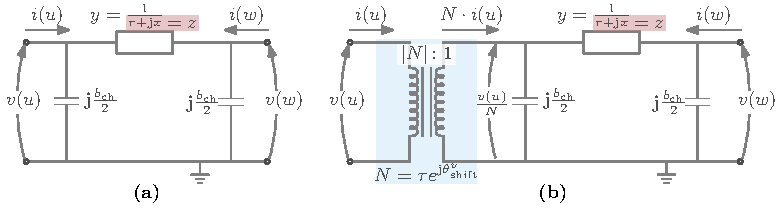
\includegraphics{foundations/figures/pi-equivalent-circuit.pdf}
    % 
    \caption[The Pi-equivalent circuit model for a transmission line]{The
    Pi-equivalent circuit represents a model of a transmission line with medium
    length. Note that this figure is partly adopted from~\textcite[p.17; Figure
    3-1]{Zimmerman2011}. (a)\&(b) The two capacitors model the transmission
    line charging~$\glssymbol{linechargingsusceptance}$, the
    impedance~\glssymbol{impedance} models the resistive behavior of a
    transmission line (red). (b) If the line represents a phase shift
    transformer then the transformer is modeled on one of the two end vertices
    (blue). The transformer (blue) is usually modeled at the vertex with the
    primary coil with a fix tap ratio~\glssymbol{tapratio} and in that
    particular case with a fix phase shift angle~\glssymbol{voltageangleshift}.
    The voltage~\glssymbol{voltage} and current~\glssymbol{current} change with
    respect to the number of windings~$\fmagnitude{N}$ on the side of the
    secondary coil. }
    % 
    \label{ch:foundations:sec:power-flow-analyses:fig:pi-equivalent-circuit}
    % 
\end{figure}
% 

For the model formulation of the previous part of this section, we used a single
line model and considered a transmission line model that is denoted
by~\emph{short transmission line representation} that neglects shunt elements
such as the shunt capacitance~\glssymbol{linechargingsusceptance} representing
the charging of a line
(see~\cref{ch:foundations:sec:power-flow-analyses:fig:pi-equivalent-circuit}).
The short transmission line representation approximates lines that are up to
80~\si{km} long by using a similar model as the RLC circuit, meaning resistance,
impedance, and capacitance are in series (see also Kirchhoff's~\nth{3}
postulate~\parencite[p.127]{Ses61}). Note that the assumption for the short
transmission line representation is reasonable, since the line charging is
negligible. Within the~\gls{ac} model terminology, we often model
the~\emph{shunt conductance} and~\emph{shunt susceptance} as elements connected
to the vertices. These elements are purely model-based theoretical elements used
to model elements such as transmission lines or synchronous condensers.
Depending on which transmission line representation is used, the shunt elements
are included or not.

For high voltage power grids it is more common to model the transmission lines
using the~\emph{medium line approximation} that includes a lumped shunt
admittance. There are two different models denoted by~\emph{pi representation}
% 
(see~\cref{ch:foundations:sec:power-flow-analyses:fig:pi-equivalent-circuit}\screen{(a)}) 
% 
and~\emph{T representation}. \textcite[p.75]{wood1996power} and applications
such as Matpower~\parencite[pp.16ff.]{Zimmerman2011} and
Pypower~\parencite{online:pypower} use the pi representation. However, there is
much more investigation in this topic as can be seen by~\textcite{CANO201771},
who introduce different transmission line representations. Note that the
standard pi representation does not include transformers (see the next
paragraph on transmission line elements).
% 
In~\cref{ch:foundations:sec:power-flow-analyses:fig:pi-equivalent-circuit}\screen{(b)},
% 
we can see the pi representation with a tap transformer. Note that there are
also~\emph{long line approximations} that are not considered in this work.
However, the pi representation is the standard model for medium length
transmission lines that are up to~$250$~\si{\km} long, which is a realistic
assumption for~\gls{ac} models. Note that most of the transmission lines are up
to 100~\si{\km} long~\parencite[p.112]{Nov12}.

The line charging
susceptance~$\glssymbol{linechargingsusceptance}(\vertexa,\vertexc)$ is a parameter of a
transmission line~$\{\vertexa,\vertexc\}\in\glssymbol{undirectededges}$ as
medium to long transmission lines tend to have an inherent capacitance. The pi
model provides us with the ability to introduce the
impedance~$\glssymbol{impedance}(\vertexa,\vertexc)$ and line charging
susceptance~$\glssymbol{linechargingsusceptance}(\vertexa,\vertexc)$ to the
admittances~$\glssymbol{admittance}(\vertexa,\vertexc)$ for all~$
\{\vertexa,\vertexc\}\in\glssymbol{undirectededges}$ and use the standard power
flow analysis as shown in the previous part of this section. The only difference
are the charge elements in the complex power equations
(see~\cref{ch:foundations:sec:power-flow-analyses:eq:complex-power-flow:pi-model}).
%
\begin{subequations}
    % \small
\begin{align}
    &\realpower(\vertexa,\vertexc) + \imgPart\cdot\reactivepower(\vertexa,\vertexc)
\\ 
% 
&=  \glssymbol{voltage}(\vertexa)
    \Big( 
        \big(
            \glssymbol{voltage}(\vertexa) - \glssymbol{voltage}(\vertexc)
        \big)
        \admittance(\vertexa,\vertexc)
    \Big)^\star 
    +
    \glssymbol{voltage}(\vertexa)
    \big(
        \glssymbol{voltage}(\vertexa)\linechargingadmittance(\vertexa, \vertexc)
    \big)^\star
\\%
%
&\begin{aligned}
&=  \fmagnitude{\glssymbol{voltage}(\vertexa)}e^{\imgPart\cdot\glssymbol{voltageangle}(\vertexa)} 
    \left( 
        \left(
            \fmagnitude{\glssymbol{voltage}(\vertexa)}e^{\imgPart\cdot\glssymbol{voltageangle}(\vertexa)} 
            - 
            \fmagnitude{\glssymbol{voltage}(\vertexc)}e^{\imgPart\cdot\glssymbol{voltageangle}(\vertexc)} 
        \right) 
        \left( 
            \conductance(\vertexa,\vertexc) 
            + 
            \imgPart\cdot\glssymbol{susceptance}(\vertexa,\vertexc) 
        \right) 
    \right)^\star 
    \\
    &\,\,\,\,- 
    \imgPart\cdot|\glssymbol{voltage}(\vertexa)|^2 \linechargingsusceptance(\vertexa,\vertexc)
\end{aligned}
\\%
% 
&\begin{aligned}
&=  \left( 
        \fmagnitude{\glssymbol{voltage}(\vertexa)}^2 
        - 
        \fmagnitude{\glssymbol{voltage}(\vertexa)}\cdot\fmagnitude{\glssymbol{voltage}(\vertexc)} 
        \cos 
        \left(
            \glssymbol{voltageangle}(\vertexa) - \glssymbol{voltageangle}(\vertexc)
        \right) 
        - 
        \imgPart\cdot\fmagnitude{\glssymbol{voltage}(\vertexa)}\fmagnitude{\glssymbol{voltage}(\vertexc)}
        \sin
        \left( 
            \glssymbol{voltageangle}(\vertexa) - \glssymbol{voltageangle}(\vertexc) 
        \right)
    \right) 
    \\
    &\times 
    \left(
            \conductance(\vertexa,\vertexc) 
            + 
            \imgPart\cdot\glssymbol{susceptance}(\vertexa,\vertexc) 
    \right)^\star 
    - \imgPart\cdot\fmagnitude{\glssymbol{voltage}(\vertexa)}^2 \linechargingsusceptance(\vertexa,\vertexc)
\end{aligned}
\end{align}
    \small
\begin{alignat}{2}
    &\glssymbol{realpower}(\vertexa,\vertexc) + \imgPart\cdot\glssymbol{reactivepower}(\vertexa,\vertexc)
\\ 
% 
&=  \glssymbol{voltage}(\vertexa)
    \Big( 
        \big(
            \glssymbol{voltage}(\vertexa) - \glssymbol{voltage}(\vertexc)
        \big)
        \glssymbol{admittance}(\vertexa,\vertexc)
    \Big)^\star 
    +
    \glssymbol{voltage}(\vertexa)
    \big(
        \glssymbol{voltage}(\vertexa)\glssymbol{linechargingadmittance}(\vertexa, \vertexc)
    \big)^\star
% \\%
% %
% &\begin{aligned}
% &=  \fmagnitude{\glssymbol{voltage}(\vertexa)}e^{\imgPart\cdot\glssymbol{voltageangle}(\vertexa)} 
%     \left( 
%         \left(
%             % \frac{1}{\imgPart\reactance\tapratio^2}
%             \fmagnitude{\glssymbol{voltage}(\vertexa)}
%             e^{\imgPart\cdot\glssymbol{voltageangle}(\vertexa)} 
%             - 
%             % \frac{1}{\tapratio\reactance e^{-\imgPart\cdot\glssymbol{voltageangle}shift} }
%             \fmagnitude{\glssymbol{voltage}(\vertexc)}
%             e^{\imgPart\cdot\glssymbol{voltageangle}(\vertexc)} 
%         \right) 
%         % \left( 
%         %     \conductance(\vertexa,\vertexc) 
%         %     + 
%         %     \imgPart\cdot\glssymbol{susceptance}(\vertexa,\vertexc) 
%         % \right) 
%         \glssymbol{linechargingadmittance}(\vertexa,\vertexc)
%     \right)^\star 
%     % \\
%     % &\,\,\,\,
%     - 
%     \imgPart\cdot\fmagnitude{\glssymbol{voltage}(\vertexa)}^2
%     \glssymbol{linechargingsusceptance}(\vertexa,\vertexc)
% \end{aligned}
\\%
% 
&\begin{aligned}
&=  \Big( 
        \fmagnitude{\glssymbol{voltage}(\vertexa)}^2 
        - 
        \fmagnitude{\glssymbol{voltage}(\vertexa)}\cdot\fmagnitude{\glssymbol{voltage}(\vertexc)} 
        \cos 
        \left(
            \glssymbol{voltageangle}(\vertexa) - \glssymbol{voltageangle}(\vertexc)
        \right) 
        - 
        \imgPart\cdot\fmagnitude{\glssymbol{voltage}(\vertexa)}\fmagnitude{\glssymbol{voltage}(\vertexc)}
        \sin
        \left( 
            \glssymbol{voltageangle}(\vertexa) - \glssymbol{voltageangle}(\vertexc) 
        \right)
    \Big) 
    \\
    &\,\,\,\,
    \cdot
    % \left(
    %         \conductance(\vertexa,\vertexc) 
    %         + 
    %         \imgPart\cdot\glssymbol{susceptance}(\vertexa,\vertexc) 
    % \right)^\star 
    \glssymbol{admittance}(\vertexa,\vertexc)^\star
    - \fmagnitude{\glssymbol{voltage}(\vertexa)}^2 \glssymbol{linechargingadmittance}(\vertexa,\vertexc)^\star
\end{aligned}
\end{alignat}
    \label{ch:foundations:sec:power-flow-analyses:eq:complex-power-flow:pi-model}
\end{subequations}
% 
for all~$(\vertexa,\vertexc)\in\glssymbol{edges}$. However, the admittance
changes a bit. Using the pi representation with transformer
(see~\cref{ch:foundations:sec:power-flow-analyses:fig:pi-equivalent-circuit}\screen{b}),
the admittance~\glssymbol{admittance} changes in the following way. Each
transformer has two different windings, one on the primary side and the other
one on the secondary side. We denote the ratio by turn ratio (or tap
ratio)~$\glssymbol{tapratio}(\vertexa,\vertexc)\coloneqq\nicefrac{\fmagnitude{
\glssymbol{voltage}(\vertexc)}} {\fmagnitude{\glssymbol{voltage}(\vertexa)}} =
\nicefrac{\glssymbol{voltage}(\vertexc)}{\glssymbol{voltage} (\vertexa)} = -
\nicefrac{\glssymbol{current}(\vertexa, \vertexc)}{\glssymbol{current} (\vertexc, \vertexa)}$ that can
be calculated by the voltage ratios of both sides.
The self-admittance is defined by~$\glssymbol{linechargingadmittance}
(\vertexa,\vertexa)\coloneqq\left(\glssymbol{admittance}(\vertexa,\vertexc) +
\imgPart\frac{\glssymbol{linechargingsusceptance}}{2}\right)\frac{1}{\glssymbol{tapratio}^2}$
and the edge admittance is defined by~$\glssymbol{linechargingadmittance}
(\vertexa,\vertexc)\coloneqq -\glssymbol{admittance}
(\vertexa,\vertexc)\frac{1}{\glssymbol{tapratio}
e^{-\imgPart\glssymbol{voltageangleshift}} }$. Note that the transformer
\emph{tap ratio}~\glssymbol{tapratio} only influences the admittance
at~\vertexa, but not at~\vertexc. However, the admittance for the edge is
symmetric apart from the sign of the exponent.

In the latter line model, we added a transformer that changed the admittance
entries only. Adding transformers or~\gls{facts} on an edge
$\{\vertexa,\vertexc\} \in \glssymbol{undirectededges}$ changes the entries of
the admittances~$\glssymbol{admittance}(\vertexa,\vertexc)$. However, it does
not influence the power grid analysis, which we describe in the following.
% 
% 
%%%%%%%%%%%%%%%%%%%%%%%%%%%%%%%%%%%%%%%%%%%%%%%%%%%%%%%%%%%%%%%%%%%%%%%%%%%%%%%%
\paragraph{Transmission Line Elements}
\label{ch:foundations:sec:power-flow-analyses:transmission-line-elements}
%%%%%%%%%%%%%%%%%%%%%%%%%%%%%%%%%%%%%%%%%%%%%%%%%%%%%%%%%%%%%%%%%%%%%%%%%%%%%%%%
% 
One possibility to model transformers or~\gls{facts} is by adjusting the entries
of the admittance matrix~$\mathbf{\admittances}$
(see~\cref{ch:foundations:sec:power-flow-analyses:eq:transmission-line-elements:admittance}).
Thus, it has no effect on the steps of the previously shown vertex-based
analysis. From~\citeauthor{Cai12}, we know that the matrix is usually
sparse~\parencite[p.17]{Cai12}. 
% 
% meaning~$\nicefrac{(\fmagnitude{\glssymbol{vertices}}+\fmagnitude{\glssymbol{edges}})}
% {\fmagnitude{\glssymbol{vertices}}^2}$
% 
The lowest density is given by a spanning forest and the highest density by a
complete graph. It is very uncommon for power grids to correspond to the latter
graph structure for more than three vertices.

An ideal in-phase transformer usually has two sides denoted by primary and
secondary side that we denote by~\vertexa and~\vertexc, respectively. Ideal
means that there is no resistance in the windings, no leaking flux, and no
hysteresis losses~\parencite[p.17]{Cai12}. Thus, the phases on both ends are
assumed to be equal meaning~$\glssymbol{voltageangle}(\vertexa) =
\glssymbol{voltageangle}(\vertexc)$. Recall from the previous paragraph that
each transformer has two different windings, one on the primary side and the
other one on the secondary side and that the turn ratio is defined by~$
\glssymbol{tapratio}(\vertexa,\vertexc)\coloneqq\nicefrac{\fmagnitude{
\glssymbol{voltage}(\vertexc)}} {\fmagnitude{\glssymbol{voltage}(\vertexa)}} =
\nicefrac{\glssymbol{voltage}(\vertexc)}{\glssymbol{voltage} (\vertexa)} = -
\nicefrac{\glssymbol{current}(\vertexa, \vertexc)}{\glssymbol{current} (\vertexc, \vertexa)}$ that can
be calculated by the voltage ratios of both sides. However, the voltage angles
at the primary and secondary coil change for a phase shift transformer. Thus, we
have an additional parameter that is called the phase angle
shift~\glssymbol{voltageangleshift} that changes the voltage angle difference
to~$\glssymbol{voltageangle}(\vertexa)
- \glssymbol{voltageangle}(\vertexc) -
  \glssymbol{voltageangleshift}(\vertexa,\vertexc)$. Thus, the ratios are
  defined by~$\nicefrac{\fmagnitude{\glssymbol{voltage}(\vertexc)}}{
\fmagnitude{\glssymbol{voltage}(\vertexa)}} =
\glssymbol{tapratio}(\vertexa,\vertexc)e^{\imgPart\glssymbol{voltageangleshift}
(\vertexa,\vertexc)}$ and~$\nicefrac{\glssymbol{current}(\vertexa,
\vertexc)}{\glssymbol{current}(\vertexc, \vertexa)} =
-\glssymbol{tapratio}(\vertexa,\vertexc)e^{-\imgPart\glssymbol{voltageangleshift}
(\vertexa,\vertexc)}$.
In~\cref{ch:foundations:sec:power-flow-analyses:eq:transmission-line-elements:admittance}
the entries of the admittance matrix~\admittanceMatrix for an edge~$
(\vertexa,\vertexc)\in\glssymbol{edges}$ are given for two different
transformers and the third setting is when there is no transformer (\ie,
standard pi representation).
% 
\begin{equation}
    \admittanceMatrix
    = 
    \begin{cases}
        \glssymbol{admittance}(\vertexa,\vertexc) \hspace{3.7cm}= 
        \glssymbol{admittance}'(\vertexa,\vertexc) &\text{No Transformer}
        \\
        \glssymbol{admittance}(\vertexa,\vertexc)\cdot \glssymbol{tapratio}
        (\vertexa,\vertexc)^2 \hspace{2.17cm}= \glssymbol{admittance}'(\vertexa,\vertexc)&
        \text{Ideal Transformer}
        \\
        \left\{
            \begin{array}{lll}
                \glssymbol{tapratio}(\vertexa,\vertexc)^2\glssymbol{admittance}
                (\vertexa,\vertexa) &= \glssymbol{admittance}'(\vertexa,\vertexa)&
                \\
                -\glssymbol{tapratio}(\vertexa,\vertexc) e^
                {-\imgPart\glssymbol{voltageangleshift}
                (\vertexa,\vertexc)}\glssymbol{admittance}
                (\vertexa,\vertexc) &= \glssymbol{admittance}'(\vertexa,\vertexc)&
                \\
                \glssymbol{admittance}(\vertexc,\vertexc) &= \glssymbol{admittance}'(\vertexc,\vertexc)&
                \\
                -\glssymbol{tapratio}(\vertexa,\vertexc)
                e^{\imgPart\glssymbol{voltageangleshift}(\vertexa,\vertexc)}
                \glssymbol{admittance}(\vertexc,\vertexa) &= \glssymbol{admittance}'(\vertexc,\vertexa)&
            \end{array}
        \right\}&\text{Phase Shift Transformer}
    \end{cases}%
    \label{ch:foundations:sec:power-flow-analyses:eq:transmission-line-elements:admittance}
\end{equation}%
% 
The self-admittances~$\glssymbol{admittance}(\vertexa,\vertexa)$ is defined by
the admittance-to-ground~$\glssymbol{admittance}(\vertexa,0)$ and the sum of the
admittances of all adjacent edges,
where~$\glssymbol{admittance}(\vertexa,\vertexc)$ is defined as above
(see~\cref{ch:foundations:sec:power-flow-analyses:eq:transmission-line-elements:self-admittance}).
%
\begin{equation}%
    \glssymbol{admittance}(\vertexa,\vertexa) = \glssymbol{admittance}(\vertexa,0) + \sum_{ 
    \vertexc\colon\{\vertexa,\vertexc\}\in\glssymbol{undirectededges} } \glssymbol{admittance}
    (\vertexa,\vertexc)\qquad\forall\vertexa\in\glssymbol{vertices}.
    % 
    \label{ch:foundations:sec:power-flow-analyses:eq:transmission-line-elements:self-admittance}
\end{equation}%
% 
This shows that the integration of transmission elements such as different line
types or transformers can be done by the admittances in the vertex-based
analysis. 
% 
% \begin{align*}
% % 
% \glssymbol{current}(\vertexa,\vertexc) =
% \tapratio(\vertexa,\vertexc)^2\admittance(\vertexa,\vertexc)\glssymbol{voltage}(\vertexa)- \tapratio
% (\vertexa,\vertexc)\admittance(\vertexa,\vertexc)\glssymbol{voltage}(\vertexc)\\
% % 
% \glssymbol{current}(\vertexc,\vertexa) =
% -\tapratio(\vertexa,\vertexc)\admittance(\vertexa,\vertexc)\glssymbol{voltage}(\vertexa)+ \admittance(\vertexa,\vertexc)\glssymbol{voltage}(\vertexc)
% % 
% \end{align*}
% % 
% For a phase shift transformer (PAR) with phase shift~\vangleshift we have
% % 
% \begin{align*}
% % 
% \frac{\glssymbol{voltage}(\vertexc)}{\glssymbol{voltage}(\vertexa)} = t(\vertexa,\vertexc) = \tapratio
% (\vertexa,\vertexc) e^{\imgPart\vangleshift}\\
% % 
% \frac{\glssymbol{current}(\vertexa,\vertexc)}{\glssymbol{current}(\vertexc,\vertexa)} = t
% (\vertexa,\vertexc)^\star = -\tapratio
% (\vertexa,\vertexc) e^{-\imgPart\vangleshift}
% % 
% \end{align*}
% % 
% In IV
% % 
% \begin{align*}
% % 
% \glssymbol{current}(\vertexa,\vertexc) = \tapratio(\vertexa,\vertexc)^2\admittance
% (\vertexa,\vertexc)\glssymbol{voltage}(\vertexa) - t(\vertexa,\vertexc)^\star\admittance
% (\vertexa,\vertexc)\glssymbol{voltage}(\vertexc)\\
% % 
% \glssymbol{current}(\vertexc,\vertexa) = -t(\vertexa,\vertexc)\admittance
% (\vertexa,\vertexc)\glssymbol{voltage}(\vertexa) + \admittance(\vertexa,\vertexc)\glssymbol{voltage}
% (\vertexc)
% % 
% \end{align*}
% 
%%%%%%%%%%%%%%%%%%%%%%%%%%%%%%%%%%%%%%%%%%%%%%%%%%%%%%%%%%%%%%%%%%%%%%%%%%%%%%%%  
\subsection{Linearized Alternating Current Power Flow Model}
\label{ch:foundations:sec:power-flow-analyses:subsec:Lin-DC-Model}
%%%%%%%%%%%%%%%%%%%%%%%%%%%%%%%%%%%%%%%%%%%%%%%%%%%%%%%%%%%%%%%%%%%%%%%%%%%%%%%%  
% 
The~\acrlong{ac} power flow models represent the standard models to analyze the
networks. However, they are non-linear, complex, and slow to compute. Since the
feasibility problem for the~\gls{ac} power flow model is already~\NP-hard on
trees~\parencite{Leh16}, an approximation of that model might be reasonable. We
go through the different steps of the approximation until we reach the
linearized~\gls{ac} power flow model that is often denoted as~\gls{dc} power
flow model. After reaching the~\gls{dc} power flow model, we will discuss the
analogies to the model for~\gls{dc} networks to understand the meaning of the
name. The~\gls{dc} assumptions of the power flow model are as follows.
% 
\crefformat{enumi}{#2\textup{\acrshort{dc}~Assumption~#1}#3\xspace}
\begin{enumerate}[({A}1)]%
    % 
    \item The series resistance is negligible, \ie, $\glssymbol{resistance}
    (\vertexa,\vertexc)\ll\glssymbol{reactance}(\vertexa,\vertexc)$ for all~$
\{\vertexa,\vertexc\}\in\glssymbol{undirectededges}$,%
    \label{ch:foundations:sec:power-flow-analyses:assumption:negligible-resistance}%
    % 
    \item the voltage angle differences~$\glssymbol{voltageangle}(\vertexa) -
    \glssymbol{voltageangle}(\vertexc)$ are
    small for all~$(\vertexa,\vertexc)\in\glssymbol{edges}$, and
    %
    \label{ch:foundations:sec:power-flow-analyses:assumption:voltage-angle-difference}%
    % 
    \item the voltage magnitudes are equal among all vertices' voltages,
    meaning~$\fmagnitude{\glssymbol{voltage}(\vertexa)} = \fmagnitude{\glssymbol{voltage}(\vertexc)}$
    for all~$\vertexa,\vertexc\in\glssymbol{vertices}$.
    %
    \label{ch:foundations:sec:power-flow-analyses:assumption:voltage-magnitude}%
\end{enumerate}%
% 
In
the~$\cref{ch:foundations:sec:power-flow-analyses:assumption:negligible-resistance}$, %
we assume that the ratio between
resistance~$\glssymbol{resistance}(\vertexa,\vertexc)$ and
reactance~$\glssymbol{reactance}(\vertexa,\vertexc)$ is very small such that we
may approximate the resistance to be~$\glssymbol{resistance}
(\vertexa,\vertexc)\approx 0$ for all
edges~$\{\vertexa,\vertexc\}\in\glssymbol{undirectededges}$. \textcite[p.20]
{Zimmerman2011} neglects the resistance~\glssymbol{resistance} and the line
charging capacitance~\glssymbol{linechargingsusceptance} meaning~$
\glssymbol{linechargingsusceptance}\approx 0$. This means that we assume that
the network is lossless as has no charging effects. Thus, all models using these
assumption are denoted as~\emph{lossless} models. If we apply this assumption to
the~\gls{ac} model this simplifies in particular the
conductance~$\glssymbol{conductance}(\vertexa,\vertexc)$
in~\cref{ch:foundations:sec:power-flow-analyses:eq:conductance} and the
susceptance~$\glssymbol{susceptance}(\vertexa,\vertexc)$
in~\cref{ch:foundations:sec:power-flow-analyses:eq:susceptance}
to~\cref{ch:foundations:sec:power-flow-analyses:eq:dc:conductance}
and~\cref{ch:foundations:sec:power-flow-analyses:eq:dc:susceptance} for all
edges~$\{\vertexa,\vertexc\}\in\glssymbol{undirectededges}$, respectively.
% 
\begin{align}%
        \glssymbol{conductance}(\vertexa,\vertexc) 
&\coloneqq
    \hphantom{-}
    \frac{
        \glssymbol{resistance}(\vertexa,\vertexc)
    }
    {
        \glssymbol{resistance}(\vertexa,\vertexc)^2 
        + 
        \glssymbol{reactance}(\vertexa,\vertexc)^2
    }
& \overset{\glssymbol{resistance} \approx 0}{=}& 
    0
& \forall \{\vertexa,\vertexc\}\in\glssymbol{undirectededges},
% 
\label{ch:foundations:sec:power-flow-analyses:eq:dc:conductance}
\\
    \glssymbol{susceptance}(\vertexa,\vertexc) 
&\coloneqq 
    -
    \frac{
        \glssymbol{reactance}(\vertexa,\vertexc)
    }
    {
        \glssymbol{resistance}(\vertexa,\vertexc)^2 
        + 
        \glssymbol{reactance}(\vertexa,\vertexc)^2
    }
& \overset{\glssymbol{resistance} \approx 0}{=}& 
    -
    \frac{
        1
    }
    {
        \glssymbol{reactance}(\vertexa,\vertexc)
    }
& \forall \{\vertexa,\vertexc\}\in\glssymbol{undirectededges}.
% 
\label{ch:foundations:sec:power-flow-analyses:eq:dc:susceptance}
\end{align}%
% 
Thus, the conductance~$\glssymbol{conductance}(\vertexa,\vertexc)$ is zero and the
susceptance~$\glssymbol{susceptance}(\vertexa,\vertexc)$ is purely reciprocal to the
reactance. This simplifies~\cref{ch:foundations:sec:power-flow-analyses:eq:real-power-flow:pqv:polar,ch:foundations:sec:power-flow-analyses:eq:reactive-power-flow:pqv:polar} to~\cref{ch:foundations:sec:power-flow-analyses:eq:assumption:resistance:1} and~\cref{ch:foundations:sec:power-flow-analyses:eq:assumption:resistance:2}, respectively.
% 
\begin{subequations}%
    \begin{align}
    \glssymbol{realpower}(\vertexa,\vertexc) 
    &\overset{(A\ref{ch:foundations:sec:power-flow-analyses:assumption:negligible-resistance})}{=} 
    \fmagnitude{\glssymbol{voltage}(\vertexa)}
    \fmagnitude{\glssymbol{voltage}(\vertexc)}
    \Big(
        \hphantom{-}\,\,\,
        \glssymbol{susceptance}(\vertexa,\vertexc)
        \sin
        \big( 
            \glssymbol{voltageangle}(\vertexa)
            -
            \glssymbol{voltageangle}(\vertexc) 
        \big) 
    \Big)
    \label{ch:foundations:sec:power-flow-analyses:eq:assumption:resistance:1}
\\
    \glssymbol{reactivepower}(\vertexa,\vertexc)
    &\overset{(A\ref{ch:foundations:sec:power-flow-analyses:assumption:negligible-resistance})}{=} 
    -
    \glssymbol{susceptance}(\vertexa,\vertexc)
    \Big(
        \fmagnitude{\glssymbol{voltage}(\vertexa)}
        \fmagnitude{\glssymbol{voltage}(\vertexc)}
        \cos
        \big( 
            \glssymbol{voltageangle}(\vertexa)
            -
            \glssymbol{voltageangle}(\vertexc) 
        \big) 
        - 
        \fmagnitude{\glssymbol{voltage}(\vertexa)}^2
    \Big) 
    % 
    \label{ch:foundations:sec:power-flow-analyses:eq:assumption:resistance:2}
\end{align}
    \label{ch:foundations:sec:power-flow-analyses:eq:assumption:resistance}
\end{subequations}%
% 
Recall from the transmission line representation
(see~\cref{ch:foundations:sec:power-flow-analyses:subsec:AC-Model}) that in
literature the standard representation of a transmission line is the pi
representation
(see~\cref{ch:foundations:sec:power-flow-analyses:fig:pi-equivalent-circuit}).

In
the~\cref{ch:foundations:sec:power-flow-analyses:assumption:voltage-angle-difference},
we assume that the voltage angle difference~$\glssymbol{voltageangle}(\vertexa)
- \glssymbol{voltageangle}(\vertexc)$ is small such that the cosine is
  approximately~$1$ (\ie, constant) and we are able to approximate the sine
  by~$\sin(x)\approx x$. The voltage angle difference---when assumed to be
  small---is at most~$30^\circ$ (\ie, $\nicefrac{\gls{pi}}{6}$) that corresponds
  to~$0.52$ radian. However, a typical value is~$15^\circ$ or even
  less~\parencite{Pur05}. Applying this assumption
  to~\cref{ch:foundations:sec:power-flow-analyses:eq:assumption:resistance:1}
  and~\cref{ch:foundations:sec:power-flow-analyses:eq:assumption:resistance:2}
  yields~\cref{ch:foundations:sec:power-flow-analyses:eq:assumption:vad:1}
  and~\cref{ch:foundations:sec:power-flow-analyses:eq:assumption:vad:2},
  respectively.
% 
\begin{subequations}%
    \begin{align}
    \glssymbol{realpower}(\vertexa,\vertexc) 
    &\overset{(A\ref{ch:foundations:sec:power-flow-analyses:assumption:voltage-angle-difference})}{=}
    \hphantom{-}
    \fmagnitude{\glssymbol{voltage}(\vertexa)}
    \fmagnitude{\glssymbol{voltage}(\vertexc)}
    % 
    \glssymbol{susceptance}(\vertexa,\vertexc)
    \big( 
        \glssymbol{voltageangle}(\vertexa)
        -
        \glssymbol{voltageangle}(\vertexc) 
    \big) 
    % 
    \label{ch:foundations:sec:power-flow-analyses:eq:assumption:vad:1}
\\
    \glssymbol{reactivepower}(\vertexa,\vertexc)
    &\overset{(A\ref{ch:foundations:sec:power-flow-analyses:assumption:voltage-angle-difference})}{=}
    -
    \fmagnitude{\glssymbol{voltage}(\vertexa)}
    \fmagnitude{\glssymbol{voltage}(\vertexc)}
    \glssymbol{susceptance}(\vertexa,\vertexc)
    +
    \fmagnitude{\glssymbol{voltage}(\vertexa)}^2
    \glssymbol{susceptance}(\vertexa,\vertexc)
    % 
    \label{ch:foundations:sec:power-flow-analyses:eq:assumption:vad:2}
\end{align}
    \label{ch:foundations:sec:power-flow-analyses:eq:assumption:vad}
\end{subequations}%
%
In
the~\cref{ch:foundations:sec:power-flow-analyses:assumption:voltage-magnitude}
the voltage magnitudes~$\fmagnitude{\glssymbol{voltage}(\vertexa)}$ for
all~$\vertexa\in\glssymbol{vertices}$ are assumed to be equal. Thus, we can
normalize all voltage magnitudes to 1~\glssymbol{pu}. The idea behind this
assumption is that the voltage range should be in a certain bound such that all
electrical devices work properly or (at least) are not damaged. The voltages
in~\glssymbol{pu} typically range in practice between~$0.95$~\glssymbol{pu}
and~$1.05$~\glssymbol{pu}~\parencite{Pur05}. Thus, the maximum voltage magnitude
difference is~$0.1$~\glssymbol{pu}.
% 
\begin{subequations}%
    \begin{align}
    \glssymbol{realpower}(\vertexa,\vertexc) 
    &\overset{(A\ref{ch:foundations:sec:power-flow-analyses:assumption:voltage-magnitude})}{=}
    % 
    \hphantom{-}
    \glssymbol{susceptance}(\vertexa,\vertexc)
    \big( 
        \glssymbol{voltageangle}(\vertexa)
        -
        \glssymbol{voltageangle}(\vertexc) 
    \big) 
    % 
    &\forall (\vertexa,\vertexc)\in\glssymbol{edges}
    % 
    \label{ch:foundations:sec:power-flow-analyses:eq:assumption:vm:1}
% \\
    % \glssymbol{reactivepower}(\vertexa,\vertexc)
    % &\overset{(A\ref{ch:foundations:sec:power-flow-analyses:assumption:voltage-magnitude})}{=}
    % - 2
    % % 
    % \glssymbol{susceptance}(\vertexa,\vertexc)
    % % 
    % &\forall (\vertexa,\vertexc)\in\glssymbol{edges}
    % 
    % \label{ch:foundations:sec:power-flow-analyses:eq:assumption:vm:2}
\end{align}
    \label{ch:foundations:sec:power-flow-analyses:eq:assumption:vm}
\end{subequations}%
%
Reformulating~\cref{ch:foundations:sec:power-flow-analyses:eq:assumption:vad:2}
into a vertex-based equation, since we do a vertex-based analysis, the reactive
power is given
in~\cref{ch:foundations:sec:power-flow-analyses:eq:how2neglectQinDC}
(derivation~\cref{app:foundations:sec:power-flow-analyses:eq:how-to-neglect-reactance-in-a-DC-network}).
% 
\begin{subequations}%
    \small
\begin{align}
    \glssymbol{reactivepower}(\vertexa)
    &
    \!\!
    \overset{(A
    \ref{ch:foundations:sec:power-flow-analyses:assumption:voltage-magnitude})
    }{=}
    \!\!
    - 
    \glssymbol{susceptance}(\vertexa,\vertexa)
    - 
    \sum_{\vertexc\colon\{\vertexa,\vertexc\}\in\glssymbol{undirectededges}}
    \glssymbol{susceptance}(\vertexa,\vertexc)
    \left(
        \fmagnitude{\glssymbol{voltage}(\vertexc)} 
        -
        \fmagnitude{\glssymbol{voltage}(\vertexa)}
    \right)
    % 
    &
    \forall\vertexa\in\glssymbol{vertices}
    % 
    \label{ch:foundations:sec:power-flow-analyses:eq:how2neglectQinDC:4}
\end{align}
    \label{ch:foundations:sec:power-flow-analyses:eq:how2neglectQinDC}
\end{subequations}%
% 
A similar transformation can be done for the real power yielding a similar
equation including the sum over all adjacent edges, but with the phase angle
differences. Note that the real and reactive power both depend on the
susceptance, but are either dependent on the voltage angle difference or on the
voltage magnitude differences, respectively. From the maximum value of the
voltage angle difference and the voltage magnitude difference, we know
that~$\glssymbol{realpower}\gg \glssymbol{reactivepower}$, which implies that we
can neglect the reactive power. The net flow at a
vertex~$\vertexa\in\glssymbol{vertices}$ is defined by~$\netflow
(\vertexa)\coloneqq\sum_{\vertexc\colon\{\vertexa,\vertexc\}\in\glssymbol{undirectededges}}
\glssymbol{realpower}(\vertexa,\vertexc)$.
% 
\begin{align}
% 
% \sum_{\vertexc\colon\{\vertexa,\vertexc\}\in\glssymbol{undirectededges}}
% \glssymbol{realpower}(\vertexa,\vertexc) 
\netflow(\vertexa)
&= 
0
&\forall\vertexa\in\glssymbol{vertices}
\setminus
(\glssymbol{generators}\cup\glssymbol{consumers})
% 
\label{ch:foundations:sec:power-flow-analyses:dc:eq:kcl}
\\
% 
-\glssymbol{realpowerdemandmax}(\vertexa)
\leq
\netflow(\vertexa)
&\leq
-\glssymbol{realpowerdemandmin}(\vertexa)
&\forall\vertexa\in\glssymbol{consumers}
% 
\label{ch:foundations:sec:power-flow-analyses:dc:eq:demand}
\\
% 
\glssymbol{realpowergenerationmin}(\vertexa)
\leq
\netflow(\vertexa)
&\leq
\glssymbol{realpowergenerationmax}(\vertexa)
&\forall
\vertexa\in\glssymbol{generators}
% 
\label{ch:foundations:sec:power-flow-analyses:dc:eq:generation}
\\
% 
\fmagnitude{\glssymbol{realpower}(\vertexa,\vertexc)}
&\leq
\glssymbol{capacity}(\vertexa,\vertexc)
&\forall
(\vertexa,\vertexc)\in\glssymbol{edges}
% 
\label{ch:foundations:sec:power-flow-analyses:dc:eq:capacity}
\\
% 
\glssymbol{susceptance}(\vertexa,\vertexc)
\cdot
\left( \glssymbol{voltageangle}(\vertexa) - \glssymbol{voltageangle}(\vertexc) -
\glssymbol{voltageangleshift}
\right) 
&= 
\glssymbol{realpower}(\vertexa,\vertexc) 
&\forall
(\vertexa,\vertexc)\in\glssymbol{edges}
% 
\label{ch:foundations:sec:power-flow-analyses:dc:eq:kvl}
\\
% 
\glssymbol{voltageangledifferencemin}(\vertexa,\vertexc)
\leq
% \deltavangle(\vertexa,\vertexc)
\glssymbol{voltageangle}(\vertexa) - \glssymbol{voltageangle}(\vertexc)
&\leq
\glssymbol{voltageangledifferencemax}(\vertexa,\vertexc)
&\forall
(\vertexa,\vertexc)\in\glssymbol{edges}
% 
\label{ch:foundations:sec:power-flow-analyses:dc:eq:angle-difference}
\end{align}
% 
The above~\crefrange{ch:foundations:sec:power-flow-analyses:dc:eq:kcl}
{ch:foundations:sec:power-flow-analyses:dc:eq:angle-difference} describe a
linearization of the~\gls{ac} model. The~\gls{dc} \acrlong{feas} is a linear
convex model that can be solved
in~$\bigO(\fmagnitude{\glssymbol{vertices}}^{2.5})$ time~\parencite{Vai89,Bar75}
and its decision problem is defined in the following box.
% 
\begingroup
    \begin{problem}[framed]{\acrlong{dc}~\acrlong{feas} $\gls{dc}~\feas
(\glssymbol{network})$}%
  Instance: & A \gls{dc} network~\dcnetworktuple.\\
  %
  Question: & Is there a feasible electrical flow complying with
  the~\crefrange{ch:foundations:sec:power-flow-analyses:dc:eq:kcl}
  {ch:foundations:sec:power-flow-analyses:dc:eq:angle-difference}?
  % 
\end{problem}%
    \label{ch:fundamentals:problems:DC_FEAS-Decision_Problem}
\endgroup
%
Note that the~$\gls{dc}~\feas(\glssymbol{network})$ constitutes a system of
linear equations that can be solved in polynomial-time.
% 
%%%%%%%%%%%%%%%%%%%%%%%%%%%%%%%%%%%%%%%%%%%%%%%%%%%%%%%%%%%%%%%%%%%%%%%%%%%%%%%%
\paragraph{Analogies to the DC Model}%
\label{ch:foundations:sec:power-flow-analyses:analogies-to-the-dc-model}
%%%%%%%%%%%%%%%%%%%%%%%%%%%%%%%%%%%%%%%%%%%%%%%%%%%%%%%%%%%%%%%%%%%%%%%%%%%%%%%%
% 
The~\gls{dc} model is defined by Ohm's Law
(\cref{ch:foundations:sec:power-flow-analyses:eq:dc:ohms-law:1}), which states
that voltage and current are directly proportional to each other. The
resistance is usually a known value representing the constant of
proportionality. The latter can be seen as a property of a conductor that is
(usually) fixed.
% 
\begin{align}
% 
\currents(\vertexa,\vertexc)
&\coloneqq
    \frac{
        \voltages(\vertexa,\vertexc)
    }{
        \resistances(\vertexa,\vertexc)
    } 
% 
\label{ch:foundations:sec:power-flow-analyses:eq:dc:ohms-law:1}
\\%
% 
&\hphantom{:}= 
    \conductances(\vertexa,\vertexc)
    \cdot
    \voltages(\vertexa,\vertexc)
% 
\label{ch:foundations:sec:power-flow-analyses:eq:dc:ohms-law:2}
\end{align}
% 
In the linearized~\gls{ac} model, the real power flow~$\glssymbol{realpower}
(\vertexa,\vertexc)$ behaves like the current~$\currents(\vertexa,\vertexc)$ in
the~\gls{dc} network
(see~\cref{ch:foundations:sec:power-flow-analyses:eq:dc:ohms-law:eq:1,ch:foundations:sec:power-flow-analyses:eq:dc:ohms-law:eq:2}).
In addition, the
susceptance~$\glssymbol{susceptance}(\vertexa,\vertexc)\coloneqq-\nicefrac{1}{\glssymbol{reactance}(\vertexa,\vertexc)}$
behaves like the electrical conductance~$\conductances
(\vertexa,\vertexc)\coloneqq\nicefrac{1}{\resistances(\vertexa,\vertexc)}$. The
voltage angle difference~$\glssymbol{voltageangledifference}
(\vertexa,\vertexc)$ behaves like the voltage~$\voltages(\vertexa,\vertexc)$ in
the~\gls{dc} network.
% 
\begin{align}
\glssymbol{realpower}(\vertexa,\vertexc)
&= 
    \glssymbol{susceptance}(\vertexa,\vertexc)
    \cdot
    \glssymbol{voltageangledifference}(\vertexa,\vertexc)
\label{ch:foundations:sec:power-flow-analyses:eq:dc:ohms-law:eq:1}
% 
\\
% 
\currents(\vertexa,\vertexc)
&= 
    \conductances(\vertexa,\vertexc)
    \cdot
    \voltages(\vertexa,\vertexc)
% 
\label{ch:foundations:sec:power-flow-analyses:eq:dc:ohms-law:eq:2}
% 
\end{align}
% 
In literature it is common to use capital letters, since in an ideal~\gls{dc}
model voltage, current and power do not change over time
(see~\cref{ch:foundations:sec:power-flow-analyses:fig:ac-vs-dc-plots}\screen{a}),
neglecting temperature and other influences over time.
% 
%%%%%%%%%%%%%%%%%%%%%%%%%%%%%%%%%%%%%%%%%%%%%%%%%%%%%%%%%%%%%%%%%%%%%%%%%%%%%%%%  
\subsection{The Voltage Normalized Lossless Real Power Flow Model -- A 
Model between AC and DC Model}
\label{ch:foundations:sec:power-flow-analyses:subsec:Sin-Model}
%%%%%%%%%%%%%%%%%%%%%%%%%%%%%%%%%%%%%%%%%%%%%%%%%%%%%%%%%%%%%%%%%%%%%%%%%%%%%%%%  
% 
In~\cref{ch:foundations:sec:power-flow-analyses:subsec:AC-Model}, we discussed
nonlinear power flow models (\gls{ac} power flow models) that are also
non-convex. The nonlinear and non-convex model makes the~\acrlong{feas}
(\gls{feas}) difficult to solve to optimality as most nonlinear solvers provide
locally optimal solutions, since they get stuck in a local optima. Thus, a
common way is to simplify the model.
In~\cref{ch:foundations:sec:power-flow-analyses:subsec:Lin-DC-Model}, we showed
how to simplify the~\gls{ac} model by linearizing it to the so called~\gls{dc}
model. Though it is not the model for the~\gls{dc} network, we could show the
analogies to it that make algorithms for the linearized~\gls{ac} model
applicable to~\gls{dc} networks.

\textcite[pp.60; Equation 1]{Don05} and~\textcite[p.1791; Equation 3.1]{Pin10}
introduced another power flow model that is either called
\emph{\textquote{lossless} model} or \emph{Sin model}. However, we denote it
as~\acrlong{sinac} (\gls{sinac}) model for a clear description and
distinction from the other models. It represents a hybrid model between
the~\gls{ac} and~\gls{dc} model. This model is not as general as
the~\gls{ac} model as it
incorporates~\cref{ch:foundations:sec:power-flow-analyses:assumption:negligible-resistance}
and~\mbox{$\cref{ch:foundations:sec:power-flow-analyses:assumption:voltage-magnitude}$,}
but more general than the~\gls{dc} model as it
neglects~$\cref{ch:foundations:sec:power-flow-analyses:assumption:voltage-angle-difference}$.
From~$\cref{ch:foundations:sec:power-flow-analyses:assumption:negligible-resistance}$,
the model is often denoted by the term \textquote{lossless}. By
introducing~\cref{ch:foundations:sec:power-flow-analyses:assumption:voltage-magnitude}
(\ie, fixing all---\ie, for all~\vertexa in~\glssymbol{vertices}---voltage
magnitudes~$\fmagnitude{\glssymbol{voltage}(\vertexa)}$ to 1~\gls{pu}), we
know from~\cref{ch:foundations:sec:power-flow-analyses:subsec:Lin-DC-Model} that
the reactive power becomes negligible.

As the previous models do, the~\gls{sinac} model incorporates the conservation
of flow (\gls{kcl};
\cref{ch:foundations:sec:power-flow-analyses:eq:model:lossless-feas:KCL-intermediate-vertex,ch:foundations:sec:power-flow-analyses:eq:model:lossless-feas:KCL-generator-vertex,ch:foundations:sec:power-flow-analyses:eq:model:lossless-feas:KCL-consumer-vertex}),
the power flow equation (\gls{kvl}-like;
\cref{ch:foundations:sec:power-flow-analyses:eq:model:lossless-feas:kvl}), and
the voltage angle difference bounds
(\cref{ch:foundations:sec:power-flow-analyses:eq:model:lossless-feas:steady-state-stability}).
The latter constraints model the steady-state
stability~\parencite[p.113]{Ver10}. Recall that~$\netflow
(\vertexa)\coloneqq\sum_{\vertexc\colon\{\vertexa,\vertexc\}\in\glssymbol{undirectededges}}
\glssymbol{realpower}(\vertexa,\vertexc)$.
% 
\begin{subequations}%
    \begin{align}
% 
\glssymbol{netflow}(\vertexa) 
&= 
0 
&\forall\vertexa\in\glssymbol{vertices}\setminus(
\glssymbol{generators}\cup\glssymbol{consumers}),
% 
\label{ch:foundations:sec:power-flow-analyses:eq:model:lossless-feas:KCL-intermediate-vertex}
% 
\\
% 
\glssymbol{realpowergenerationmin}(\vertexa)\leq\glssymbol{netflow}
(\vertexa)&\leq\glssymbol{realpowergenerationmax}(\vertexa)
&\forall\vertexa\in\glssymbol{generators},
\label{ch:foundations:sec:power-flow-analyses:eq:model:lossless-feas:KCL-generator-vertex}\\%
% 
-\glssymbol{realpowerdemandmax}(\vertexa)\leq\glssymbol{netflow}(\vertexa)&\leq
-\glssymbol{realpowerdemandmin}
(\vertexa)
&\forall\vertexa\in\glssymbol{consumers}.
\label{ch:foundations:sec:power-flow-analyses:eq:model:lossless-feas:KCL-consumer-vertex}%
% 
\\
%
\glssymbol{susceptance}(\vertexa,\vertexc)\cdot
\sin\big(
    \glssymbol{voltageangle}(\vertexa)-\glssymbol{voltageangle}(\vertexc)
\big) 
&= 
\glssymbol{flow}(\vertexa,\vertexc)
&\forall(\vertexa,\vertexc)\in\glssymbol{edges}
% 
\label{ch:foundations:sec:power-flow-analyses:eq:model:lossless-feas:kvl}
\\
% 
\fmagnitude{
    \glssymbol{voltageangle}(\vertexa)-\glssymbol{voltageangle}(\vertexc)
}
&\leq 
\frac{\gls{pi}}{2} 
&\forall(\vertexa,\vertexc)\in\glssymbol{edges}
\label{ch:foundations:sec:power-flow-analyses:eq:model:lossless-feas:steady-state-stability}
% 
\\
\fmagnitude{\glssymbol{flow}(\vertexa,\vertexc)}&\leq\glssymbol{capacity}
(\vertexa,\vertexc)&\forall
(\vertexa,\vertexc)\in\glssymbol{edges}
\label{ch:foundations:sec:power-flow-analyses:eq:model:lossless-feas:capacity}
% 
\end{align}
    \label{ch:foundations:sec:power-flow-analyses:eq:model:lossless-feas}
\end{subequations}%
% 
Recall that we look at the real part~$\real{\cdot}$ of the power flow model and
that the angle differences are restricted to~$\left[-\nicefrac{\gls{pi}}{2};
\nicefrac{\gls{pi}}{2}\right]$.
The~\crefrange{ch:foundations:sec:power-flow-analyses:eq:model:lossless-feas:kvl}
{ch:foundations:sec:power-flow-analyses:eq:model:lossless-feas:capacity} can be
reformulated
to~\cref{ch:foundations:sec:power-flow-analyses:eq:model:lossless-feas:reformulation:1,ch:foundations:sec:power-flow-analyses:eq:model:lossless-feas:reformulation:2},
respectively. Note
that~\cref{ch:foundations:sec:power-flow-analyses:eq:model:lossless-feas:reformulation:1}
is just a reformulation
of~\cref{ch:foundations:sec:power-flow-analyses:eq:model:lossless-feas:kvl}.
Since the sine for~$\pm\nicefrac{\gls{pi}}{2}$ (voltage angle difference restriction;
\cref{ch:foundations:sec:power-flow-analyses:eq:model:lossless-feas:steady-state-stability})
is~$\pm 1$ the voltage angle difference is the minimum of~$1$ and~$
\glssymbol{reactance}(\vertexa,\vertexc)\cdot\glssymbol{capacity}(\vertexa,\vertexc)$.
% 
\begin{align}
% 
\glssymbol{voltageangle}(\vertexa) - \glssymbol{voltageangle}(\vertexc) &=
\arcsin\big(\glssymbol{reactance}
(\vertexa,\vertexc)\cdot\glssymbol{flow}(\vertexa,\vertexc)\big) & 
(\vertexa,\vertexc)\in\glssymbol{edges},
% 
\label{ch:foundations:sec:power-flow-analyses:eq:model:lossless-feas:reformulation:1}
% 
\\
% 
\fmagnitude{\glssymbol{voltageangle}(\vertexa)-\glssymbol{voltageangle}
(\vertexc)}&\leq \arcsin(\min\{1,\glssymbol{reactance}
(\vertexa,\vertexc)\cdot\glssymbol{capacity}(\vertexa,\vertexc)\}) & 
(\vertexa,\vertexc)\in\glssymbol{edges}.
%
\label{ch:foundations:sec:power-flow-analyses:eq:model:lossless-feas:reformulation:2}
% 
\end{align}
% 
\cref{ch:foundations:sec:power-flow-analyses:eq:model:lossless-feas:reformulation:2}
incorporates the voltage angle differences
(\cref{ch:foundations:sec:power-flow-analyses:eq:model:lossless-feas:steady-state-stability})
and the capacity constraint
(\cref{ch:foundations:sec:power-flow-analyses:eq:model:lossless-feas:capacity}).
\textcite[p.114; Lemma 4.2.1 \& Theorem 4.2.2]{Ver10} showed the uniqueness of a
feasible power flow in the~\gls{sinac}-model.
% 
% with the assumption for~$
% \glssymbol{voltageangle}(\vertexa)
% - \glssymbol{voltageangle} (\vertexc) - h (\vertexa,\vertexc,\glssymbol{flow}
%   (\vertexa,\vertexc) )$ that the
%   function~$h\colon\glssymbol{vertices}\times\glssymbol{vertices}\times\reals\to\reals$
%   is skew-symmetric and strictly monotonic increasing, and that the
%   capacity~$\glssymbol{capacity} (\vertexa,\vertexc)\geq0$. 
% 
Note that in general the power grid has no hard capacities. The thermal line
limits for the calculation is usually to maintain the safety of the lines such
that they are not overheating. Since the power flows are unique, we can neglect
the capacity constraints for the~\acrlong{feas}. Note that we prove and use the
same observation in~\cref{ch:network-analysis} in a different way. When
neglecting the capacity constraint the right-hand side
of~\cref{ch:foundations:sec:power-flow-analyses:eq:model:lossless-feas:reformulation:2}
becomes~$\arcsin(1)$. The decision problem of the~\gls{sinac} is defined in the
following problem box.
% 
\begingroup
    \begin{problem}[framed]{\acrlong{sinac}~\acrlong{feas}}%
  % 
  Instance: & A~\gls{sinac} network~\dcnetworktuple.\\
  % 
  Question: & Is there a feasible electrical flow complying
  with~\crefrange{ch:foundations:sec:power-flow-analyses:eq:model:lossless-feas:KCL-intermediate-vertex}{ch:foundations:sec:power-flow-analyses:eq:model:lossless-feas:capacity}?
  % 
  % 
\end{problem}%
    \label{ch:fundamentals:problems:SINAC_FEAS-Decision_Problem}
\endgroup
% 
Note that the model is non-linear and non-convex~\parencite{Ver10}.
% 
On general graphs, \textcite{Ver10} shows that the capacitated version
of~\gls{sinac} is \NP-complete
(see~\cref{ch:foundations:sec:power-flow-analyses:subsec:Sin-Model}). In this
work they do a reduction from one-in-three 3-SAT, where each clause has exactly
one true literal. \textcite{Bie19} extended that to strong
\NP-hardness. 

For the~\gls{sinac} model 
(\cref{ch:foundations:sec:power-flow-analyses:subsec:Sin-Model}), the
feasibility problem can be solved in polynomial time in the size of the network
and~$\nicefrac{1}{\epsilon}$ for graphs with bounded tree-width and any given
tolerance~$\epsilon$.
% 
%%%%%%%%%%%%%%%%%%%%%%%%%%%%%%%%%%%%%%%%%%%%%%%%%%%%%%%%%%%%%%%%%%%%%%%%%%%%%%%%  
\subsection{Alternating vs. Direct Current Model}
\label{ch:foundations:sec:power-flow-analyses:subsec:AC-vs-DC-Model}
%%%%%%%%%%%%%%%%%%%%%%%%%%%%%%%%%%%%%%%%%%%%%%%%%%%%%%%%%%%%%%%%%%%%%%%%%%%%%%%%  
% 
\begin{figure}
[t!]%TODO :
% https://opentextbc.ca/physicstestbook2/chapter/reactance-inductive-and-capacitive/
    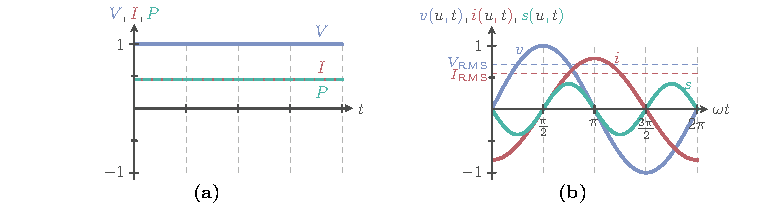
\includegraphics{foundations/figures/ac-vs-dc.pdf}
    % 
    \caption[Difference between the~\gls{ac} and~\gls{dc} model]{The
        plots for~\gls{ac} and~\gls{dc} models differ in their
        \screentextcolor{COMPLEXPOWER}{power}, \screentextcolor{CURRENT}
        {current} and
        \screentextcolor{VOLTAGE}{voltage} curves. (a) The curves of the
        linearized~\acrshort{ac} model can be interpreted like the curves of
        the~\gls{dc} model as constant functions over time. Thus,
        % 
        \screentextcolor{COMPLEXPOWER}{power~$P$}, 
        % 
        \screentextcolor{CURRENT}{current~$I$},
        % 
        and \screentextcolor{VOLTAGE}{voltage~$V$} 
        % 
        are time-independent functions. 
        (b) The~\gls{ac} model consists of sinusoid functions. The 
        % 
        \screentextcolor{COMPLEXPOWER}{instantaneous power~$
        \glssymbol{complexpower}(
        \screentextcolor{TIMESTAMP}{\vertexa}, \screentextcolor{TIMESTAMP}
        {\glssymbol{timestamp}})$},
        % 
        \screentextcolor{CURRENT}{current~$\glssymbol{current}(
        \screentextcolor{TIMESTAMP}{\vertexa}, \screentextcolor{TIMESTAMP}
        {\glssymbol{timestamp}})$},
        and
        % 
        \screentextcolor{VOLTAGE}{voltage~$\glssymbol{voltage}(
        \screentextcolor{TIMESTAMP}{\vertexa}, \screentextcolor{TIMESTAMP}
        {\glssymbol{timestamp}})$} are functions over time. The~\acrlong{rms} (\gls{rms})
        of voltage~\glssymbol{voltagerms} and current~\glssymbol{currentrms} are
        represented by the dashed-colored horizontal lines.}
    % 
    \label{ch:foundations:sec:power-flow-analyses:fig:ac-vs-dc-plots}
\end{figure}
% 
Historically, the question of whether~\gls{ac} or~\gls{dc} would be used arose
in the 1800s. There was a competition between two companies of Thomas Edison and
George Westinghouse that developed and spread the use of~\gls{dc} and~\gls{ac},
respectively. This competition is also known as \textquote{war of the currents}.
In the end~\gls{ac} imposed, since the first transformers were invented
for~\gls{ac}, allowing a simple change in voltage level and long distance
transmission as well as usage of electricity in households. The first long
distance transmission of three-phase~\gls{ac} was in 1891. It is impressive that
the first pure~\gls{dc} transformer was invented in 1976, since technologies
such as semiconductors had been developed. Nowadays, the question arises in
terms of distribution systems~\parencite{Ham07}.

However, if we look at the current power grid, we mainly have an~\gls{ac} power
grid with a few~\gls{hvdc} lines. So we focus on the question of whether our
model assumptions are reasonable and when the errors would become significant.
Recall that the~\gls{dc} power flow model introduces three assumptions (\gls{dc}
Assumptions~\ref{ch:foundations:sec:power-flow-analyses:assumption:negligible-resistance}--\ref{ch:foundations:sec:power-flow-analyses:assumption:voltage-magnitude})
that simplify the~\gls{ac} power flow to a~\gls{dc} power flow model. The
question of when the~\gls{dc} model is useful, thus, depends on three
parameters: resistance of the lines, voltage angle differences, and voltage
magnitude deviations. An evaluation that tests the three assumptions is given
by~\textcite{Pur05}.

The~\gls{tso}{s} usually say that the resistance of the transmission network is
negligible. This statement is basically covered
in~$\cref{ch:foundations:sec:power-flow-analyses:assumption:negligible-resistance}$.
The transmission network in Germany has voltages of 110~\gls{kv}, 220~\gls{kv},
and 380~\gls{kv}. These voltage layers define the high voltage level. The higher
the voltage the lower the current and thus, the lower the influence of the
resistance
(see~\cref{ch:foundations:sec:power-flow-analyses:eq:complex-power-flow:pqv:rectangular:2,ch:foundations:sec:power-flow-analyses:eq:dc:ohms-law:1}).
So our expectation would be that this assumption mainly depends on the voltage
level and on the line resistances. \textcite[p.4]{Pur05} show that for the
Belgian grid with voltage levels of~$70$~\gls{kv}, $150$~\gls{kv},
$220$~\gls{kv}, and~$380$~\gls{kv} the~$\nicefrac{\reactances}{\resistances}$
ratio ranges from~$0.8$ for the~$70$~\gls{kv} voltage level to~$12.5$ for
the~$380$~\gls{kv} voltage level. The real power estimation error (that
increases with increasing resistance) for these voltage levels is less
than~$5\%$ and for the~$380~\gls{kv}$ power grid drops below~$2.5\%$. Both
errors are small and thus, the resistance for
such~$\nicefrac{\reactances}{\resistances}$ ratios in high voltage levels is
negligible.% This particularly means that for high-voltage levels the resistance is
% the main factor.\franzi{Was wollte ich damit sagen???}

The~\cref{ch:foundations:sec:power-flow-analyses:assumption:voltage-angle-difference}
assumes that the voltage angle difference is small enough such that the sine
function is negligible. The system's stability is guaranteed in the range of~$
[-\nicefrac{\gls{pi}}{2};\nicefrac{\gls{pi}}{2}]$. However, $30^\circ$ or~$[ -
\nicefrac{\gls{pi}}{6};\nicefrac{\gls{pi}}{6} ]$ is the range where the sine can be
approximated by~$\sin(x) = x$. Thus, if the difference is within this range, the
real power error should be small. \textcite[p.2]{Pur05} evaluate for the Belgian
power grid with voltages ranging from~$70$~\gls{kv} to~$380$~\gls{kv} that the
highest voltage angle difference was~$7^\circ$ and in~$94\%$ of the lines it was
less than~$2^\circ$. One explanation is that the inductive and conductive
properties of an edge are quite small. However, the lines inductive property is
usually slightly higher, though for long distances the capacitive property
increases (see the transmission line representation section
in~\cref{ch:foundations:sec:power-flow-analyses:subsec:AC-Model} on
Page~\pageref{ch:foundations:sec:power-flow-analyses:transmission-line-representation}).

The last
assumption---\cref{ch:foundations:sec:power-flow-analyses:assumption:voltage-magnitude}\!\!---is
about a flat voltage profile, \eg, all voltages are equal to~$1$~\glssymbol{pu}.
If there is a voltage deviation then this would automatically lead to a voltage
difference that is simply not modeled in the~\gls{dc} model. The real power
error increases with increasing voltage deviation~\parencite[p.4; Figure
7]{Pur05}. Thus, a flat voltage profile is important but difficult to establish
in power grids.  %\franzi{flat voltage profile means that the standard deviation
% < 0.01}

This particularly means that the most critical assumption is the flat voltage
profile. The others can be at least established quite well in a high voltage
power grid. However, flat voltage profiles are difficult to establish and thus,
the results have to be carefully interpreted in terms of an~\gls{ac} power
grid. However, this discussion also shows that the more complex Sin-model
including the sine function might be a more realistic model, but that the
assumption is not critical for the real power error and thus, it might increase
the complexity unnecessarily. However, from a theoretical perspective this
model is quite interesting as the feasibility problem is already strongly
\NP-hard~\textcite{Bie19}.
% 
%%%%%%%%%%%%%%%%%%%%%%%%%%%%%%%%%%%%%%%%%%%%%%%%%%%%%%%%%%%%%%%%%%%%%%%%%%%%%%%%
\paragraph{Problems}%
\label{ch:foundations:sec:power-flow-analyses:problems}%
%%%%%%%%%%%%%%%%%%%%%%%%%%%%%%%%%%%%%%%%%%%%%%%%%%%%%%%%%%%%%%%%%%%%%%%%%%%%%%%%
% 
The~\gls{ac} feasibility problem is a subproblem of many
optimization problems such as the~\acrlong{tnep} (\gls{tnep}) problem, 
the~\acrlong{otsp} (\gls{otsp}) and
the~\acrlong{mpfp} (\gls{mpfp}).

% the~\acrlong{edp} (\gls{edp}), the~\acrlong{ucp} (\gls{ucp})
The~\acrlong{edp} (\gls{edp}) minimizes the total cost represented by the sum of
all generator cost functions~\cost. It is the simplest problem formulation that
checks whether demand and supply match by abstracting from the power grid and
incorporates the energy balance equation, and the generator constraints
(see~\cref{ch:foundations:sec:power-flow-analyses:eq:network:bounds:real-power-injection,ch:foundations:sec:power-flow-analyses:eq:network:bounds:reactive-power-injection}).
After adding the power grid specifics, the problem is called either~\gls{ac}
or~\gls{dc}~\acrlong{opfp} (\gls{opfp}). All the problems mentioned so far have
continuous variables only.
% 
In terms of planning problems, we introduce integer or binary variables. The
most commonly known problems for finding an optimal topology are~\gls{tnep},
\gls{otsp}, and \gls{mtsfp}.
%  
% % 
% %%%%%%%%%%%%%%%%%%%%%%%%%%%%%%%%%%%%%%%%%%%%%%%%%%%%%%%%%%%%%%%%%%%%%%%%%%%%%%%%
% \section{Experimental Setup}\label{ch:foundations:sec:experimental-setup}
% %%%%%%%%%%%%%%%%%%%%%%%%%%%%%%%%%%%%%%%%%%%%%%%%%%%%%%%%%%%%%%%%%%%%%%%%%%%%%%%%  

% \paragraph{Methodology} TODO
% -c++
% -gcc and flags


% \paragraph{Benchmark Data} TODO
% - Table about the Instance, Electrical network, Number of Vertices and number of
% edges


% % 
% \begin{table}[t!]
%     \centering
%     \input{foundations/tables/tbl-benchmarkCases-powerGrid.tex}
%     % 
%     \caption{
%     Overview of the~\gls{ieee} instances used in this work. The table shows the
%     instance name, the power grid it represents, the number of vertices~$
%     \fmagnitude{\glssymbol{vertices}}$, the number of edges~$\fmagnitude{\glssymbol{edges}}$, the
%     number of generators~$\fmagnitude{\generators}$, and the number of~$
%     \fmagnitude{\consumers}$.
%     % 
%     }
%     % 
%     \label{ch:foundations:tbl:load-flow-bus-specification}
% \end{table}

% \paragraph{Implementation Details} TODO
%%%%%%%%%%%%%%%%%%%%%%%%%%%%%%%%%%%%%%%%%%%%%%%%%%%%%%%%%%%%%%%%%%%%%%%%%%%%%%%%
\Chapter{
% 
    The Direct Current Feasibility Problem
% 
}{
% 
    An Algorithmic Approach to Computing Electrical Flows
% 
}{
% 
    \footnote{I would like to thank especially Matthias Wolf and Torsten
    Ueckerdt for questions, discussions, and comments. In addition, I
    would like to thank Marc Timme for some initial conversations, his time,
    and that he encouraged me (more or less) to write this chapter. }
% 
}
\label{ch:network-analysis}
\glsresetall
%%%%%%%%%%%%%%%%%%%%%%%%%%%%%%%%%%%%%%%%%%%%%%%%%%%%%%%%%%%%%%%%%%%%%%%%%%%%%%%% 
%
The~\acrlong{ac}~\acrlong{feas} (\gls{ac} \gls{feas};
see~\cref{ch:foundations:sec:power-flow-analyses:subsec:AC-Model})
and~\acrlong{dc}~\acrlong{feas} (\gls{dc} \gls{feas};
see~\cref{ch:foundations:sec:power-flow-analyses:subsec:Lin-DC-Model}) are
subproblems of most power grid related problems such as switching
(see~\cref{ch:switching}) and ideal~\gls{facts} placement (see~\cref{ch:facts}).
In this chapter, we formalize the operation of the power grid in such a way that
we are able to develop algorithmic approaches for the electrical flow
computation. With the latter formulations, we are able to develop better
algorithms for problems that incorporate the electrical flow computation as a
subproblem. Recall that one of the first persons who increased the knowledge
in~\gls{dc}~\gls{feas} was Kirchhoff~\parencite{Kir47}, who formalized the
electrical flow and introduced structural properties.

In~\cref{ch:foundations:sec:power-flow-analyses}, we described different models
and approximations to analyze the network by calculating the power flow, which
we call more generally electrical flow. In this chapter, we focus on
the~\acrlong{dc} \acrlong{feas} (\gls{dc}~\gls{feas}; commonly known
as~\acrlong{pf}; in short~\gls{pf}) and the~\gls{dc}~\acrlong{mpfp}
(\gls{dc}~\gls{mpfp}). We describe their mathematical models using different
formulations and give some structural insights that will be important to develop
algorithms for~\gls{dc}~\gls{feas} and~\gls{dc}~\gls{mpfp}
(see~\cref{ch:foundations:sec:power-flow-analyses:subsec:Lin-DC-Model}). Note
that one of the first algorithms---though with exponential running time---to
compute electrical flows uses spanning trees
(see~\cref{ch:network-analyzes:sec:mathematical-model:lem:current_edge_from_a_to_b};
\parencite{Ses61,Sha87}). We describe the latter
algorithm~\parencite{Ses61,Sha87} briefly
in~\cref{ch:network-analyzes:sec:mathematical-model}. This algorithm was used
by~\textcite{Fel13} to construct a squaring of a
rectangle~\parencite[pp.17ff.]{Fel13}. \citeauthor{Fel13} shows that the flow of
a graph that represents such a squaring of a rectangle is equivalent to a
solution of an integer~\gls{dc}~\gls{feas}, meaning all flows have to be
integral. Since this problem uses integral electrical flows (\ie, the flow is a
function~$
    % 
    \glssymbol{flow}
    \colon
    \glssymbol{edges}
    \to
    \integers
    % 
$), we usually cannot apply an~\gls{lp}
from~\cref{ch:foundations:sec:power-flow-analyses:subsec:Lin-DC-Model}, but have
to use an~\gls{ilp}. In general solving~\gls{ilp}s is~\NP-hard~\parencite[p.245;
MP1]{Gar79}. However, if the solution space has some properties, it is possible
to solve it with other techniques and algorithms in polynomial time. One
possibility would be to relax the variables of~\gls{dc}~\gls{feas}, which means
that a solution of an~\gls{lp} yields an integral solution. However, we show
that this technique does not necessarily result in an integral flow. However, if
we do not have a fixed generation, a fixed demand, and neglect the capacities,
meaning~$\glssymbol{capacity}\equiv\infty$, but ask for a generation and demand
such that we get integral electrical flows, we can make use of some properties
of the solution space. 
% This particular result shows us that there are integral
% electrical flows, which we will use for the runtime estimations.
% 
% However, we show that this is possible for that particular case,
% since the corners of the polytope (\ie, of the solution space) are on integral
% coordinates and get a~$\bigO(\fmagnitude{\glssymbol{vertices}}^{2.5})$
% algorithm~\parencite{Vai89,Bar75} for general graphs and
% an~$\bigO(\fmagnitude{\glssymbol{vertices}})$ algorithm for planar graphs.

In~\cref{ch:network-analyzes:sec:reduction-transformation-rules}, we first give
an overview over known transformation and contraction rules. In the end
of~\cref{ch:network-analyzes:sec:reduction-transformation-rules}, we give an
algorithm for the~\source-\sink-\gls{dc}~\gls{feas} and -\gls{mpfp} on planar
biconnected graphs that runs in~$\bigO(\fmagnitude{\glssymbol{vertices}}^3)$
time. Recall that~\gls{dc}~\gls{feas} and~\gls{mpfp} can be formulated as a
linear system of equations and an~\gls{lp}, respectively, that can be solved 
in~$\bigO(\fmagnitude{\glssymbol{edges}}^{2.5})$ time~\parencite{Vai89,Bar75}.
% 
Thus, using the contraction and transformation rules in the fashion described
in~\cref{ch:network-analyzes:sec:reduction-transformation-rules} does not yield
an algorithm that has a better running time than the known mathematical methods.
However, it gives some structural information.

While restricting our graphs to biconnected planar \source-\sink-graphs, we
develop an algorithm that transforms the formulation given
in~\cref{ch:foundations:sec:power-flow-analyses}
and~\cref{ch:network-analyzes:sec:mathematical-model} to an equivalent
formulation of~\emph{simultaneous flows}
(\cref{ch:network-analyzes:simultaneous-flow-representation}). For this
formulation, we are able to develop an algorithmic approach for~\source-\sink-
\gls{dc}~\gls{feas} and -\gls{mpf} algorithm for biconnected graphs
(\cref{ch:network-analyzes:sec:algorithm}) that can be extended to an algorithm
for multiple sources and multiple sinks on planar graphs by using the
superposition principle for linear physical systems.
% 
% 
%%%%%%%%%%%%%%%%%%%%%%%%%%%%%%%%%%%%%%%%%%%%%%%%%%%%%%%%%%%%%%%%%%%%%%%%%%%%%%%
\section[A Mathematical Model for the Feasibility Problem of Electrical Flows]{
A Mathematical Model for the \protect\linebreak{Feasibility Problem of Electrical Flows}} 
% 
\label{ch:network-analyzes:sec:mathematical-model}
%%%%%%%%%%%%%%%%%%%%%%%%%%%%%%%%%%%%%%%%%%%%%%%%%%%%%%%%%%%%%%%%%%%%%%%%%%%%%%%
% 
\textcite[p.13]{Cai12} give the structural hint that power grids are often
planar. Note that this might not be true in general. In addition, power grids
are quite sparse.
% 
The electrical network's topology is described by a bidirected
graph~$\glssymbol{graph} = (\glssymbol{vertices},\glssymbol{edges})$,
where~\glssymbol{vertices} is the set of vertices representing the buses (\ie,
line junctions), and~\glssymbol{edges} is the set of edges representing the
lines or cables (the conventional name is branch). Though the underlying graph
is undirected~\parencite[p.13]{Cai12}, we are always able to direct its
edges~$\{\vertexa,\vertexc\}\in
\glssymbol{undirectededges}$ by inserting two edges in opposite direction~$
(\vertexa,\vertexc), (\vertexc,\vertexa)\in\glssymbol{edges}$. Introducing the
direction is motivated by the electrical network's direction that is usually
defined by the voltage or current source representing the~\emph{reference}
vertex (also known as~\emph{slack} or~\emph{datum};
see~\cref{ch:foundations:tbl:load-flow-bus-specification} on
Page~\pageref{ch:foundations:tbl:load-flow-bus-specification}). The direction is
used for notational convenience and for electrical networks that
are~\emph{nonreciprocal}. Nonreciprocal electrical networks have components on
their edge that have a predefined direction such as diodes. However, in our case
the electrical network is reciprocal (also known as \emph{bilateral}) and thus,
the flow on each edge is allowed to flow in both directions. The underlying
graph is undirected, and we define for notational convenience the
set~\glssymbol{undirectededges} of undirected edges
by~$
    % 
    \glssymbol{undirectededges} 
    = 
    \{
        \undirectededge
        \mid
        \edge
        \in
        \glssymbol{edges}
    \}
    % 
$, \ie, $
% 
\makeUndirected{(\vertexa,\vertexc)} 
= 
\makeUndirected{(\vertexc,\vertexa)} 
= 
\{\vertexa,\vertexc\}
% 
$.

Each edge has a thermal limit and a susceptance that are represented by the
functions~$\glssymbol{capacity}\colon\glssymbol{undirectededges}\to\reals$
and~$\glssymbol{susceptance}\colon\glssymbol{undirectededges}\to\reals$,
respectively. The set~\glssymbol{generators} of generators represents the energy
sources and the demands are represented by a set~\glssymbol{consumers} of
consumers. Without loss of generality, we assume
that~$
    % 
    \glssymbol{generators}
    \cap
    \glssymbol{consumers}
    =
    \emptyset
    % 
$ and~$
    % 
    \glssymbol{generators}
    \cup
    \glssymbol{consumers}
    \subseteq
    \glssymbol{vertices}
    % 
$. An \emph{electrical network} is defined by a tuple~$\dcnetworktuple$ with
minimum and maximum generation~$
    % 
    \glssymbol{realpowergenerationmin},
    \glssymbol{realpowergenerationmax}
    \colon
    \glssymbol{vertices}
    \to
    \posreals
    \cup
    \{\infty\}
    % 
$, and minimum and maximum demand~$
    % 
    \glssymbol{realpowerdemandmin},
    \glssymbol{realpowerdemandmax}
    \colon
    \glssymbol{vertices}
    \to
    \posreals
    \cup\{\infty\}
    % 
$, respectively. In general, we distinguish between \emph{bounded} (\ie, $
    % 
    \vertexa
    \in
    \glssymbol{generators}
    \colon
    \glssymbol{realpowergenerationmax}(\vertexa)
    <
    \infty
    % 
$ and $
    % 
    \vertexa
    \in
    \glssymbol{consumers}
    \colon
    \glssymbol{realpowerdemandmax}(\vertexa)
    <
    \infty
    % 
$), \emph{unbounded} (\ie, $
    % 
    \glssymbol{realpowergenerationmax}
    \equiv
    \glssymbol{realpowerdemandmax}
    \equiv
    \infty
    % 
$), and \emph{exact} (\ie, $
    % 
    % \vertexa
    % \in
    % \glssymbol{generators}
    % \colon
    \glssymbol{realpowergenerationmin}%(\vertexa) 
    \equiv
    \glssymbol{realpowergenerationmax}%(\vertexa)
    % 
$ and~$
    % 
    % \vertexa
    % \in
    % \glssymbol{consumers}
    % \colon
    \glssymbol{realpowerdemandmin}%(\vertexa)
    \equiv
    \glssymbol{realpowerdemandmax}%(\vertexa)
    % 
$) networks.

The power is defined by current and voltage functions. These functions over time
map an edge and a point in time to voltage and current values
(see~\cref{ch:foundations:sec:power-flow-analyses:subsec:AC-Model}). However, in
this work we focus on \emph{steady-state} systems that are invariant and thus,
bind the functions to one particular timestamp. The latter means that all
functions become time independent.
%
A \emph{flow} is a function~$
    % 
    \glssymbol{flow}
    \colon
    \glssymbol{edges}
    \to
    \reals,
    (\vertexa,\vertexc)
    \mapsto
    \glssymbol{flow}(\vertexa,\vertexc)
    % 
$. A flow complies with the skew-symmetry
property~$
    % 
    \glssymbol{flow}(\vertexa,\vertexc) 
    = 
    -\glssymbol{flow}(\vertexc,\vertexa)
    % 
$ for all~$(\vertexa,\vertexc)\in\glssymbol{edges}$. The \emph{net flow} at a
vertex~$\vertexa\in\glssymbol{vertices}$ is defined by~$
    % 
    \glssymbol{netflow}(\vertexa)
    \coloneqq
    \sum_{
        \{\vertexa,\vertexc\}
        \in
        \glssymbol{undirectededges}
    }
    \glssymbol{flow}(\vertexa,\vertexc)
    % 
$. We define the \emph{flow value}~$
    % 
    \glssymbol{flowvalue}(\glssymbol{network},\glssymbol{flow})
    % 
$ to be the sum of all generator excesses~$
    % 
    \sum_{
        \vertexa
        \in
        \glssymbol{generators}
    }
    \glssymbol{netflow}(\vertexa)
    % 
$.

The behavior of voltage and current in the classical physics are described by
the Kirchhoff's laws~\parencite{Kir47}\parencite[p.120; Definition 6-1]{Ses61}.
Since we are interested in power flows while using a linearization of
an~\acrshort{ac} power flow (known as~\gls{dc}~\gls{feas}), we map~\gls{dc}
currents~$\current$ to real power~$
\glssymbol{realpower}$, which we denote by~$\glssymbol{flow}$
and~\gls{dc} voltage~$\voltage$ to voltage angle
differences~$\glssymbol{voltageangledifference}$ 
(see~\cref{ch:foundations:sec:power-flow-analyses:subsec:Lin-DC-Model} on
Page~\pageref{ch:foundations:sec:power-flow-analyses:analogies-to-the-dc-model}).
% 
%%%%%%%%%%%%%%%%%%%%%%%%%%%%%%%%%%%%%%%%%%%%%%%%%%%%%%%%%%%%%%%%%%%%%%%%%%%%%%%%
\paragraph{\acrlong{kcl} (\gls{kcl})}%
\label{ch:network-analyzes:sec:mathematical-model:kcl-flow}%
%%%%%%%%%%%%%%%%%%%%%%%%%%%%%%%%%%%%%%%%%%%%%%%%%%%%%%%%%%%%%%%%%%%%%%%%%%%%%%%%
% 
The first law is called the \emph{\acrlong{kcl}}~(\gls{kcl};
\crefrange{ch:network-analyzes:sec:mathematical-model:eq:KCL-intermediate-vertex}{ch:network-analyzes:sec:mathematical-model:eq:KCL-consumer-vertex})
and describes that the power entering a vertex~$\vertexa\in\glssymbol{vertices}$
is equal to the power exiting~\vertexa. This is equivalent to the conservation
of flow in graph theory.
%
\begin{align}%
% 
\glssymbol{netflow}(\vertexa) &= 0
&\forall\vertexa\in\glssymbol{vertices}\setminus
(\glssymbol{generators}\cup\glssymbol{consumers}),
\label{ch:network-analyzes:sec:mathematical-model:eq:KCL-intermediate-vertex}
\\%
% 
\glssymbol{realpowergenerationmin}(\vertexa)
\leq\glssymbol{netflow}(\vertexa)
&\leq\glssymbol{realpowergenerationmax}(\vertexa) 
&\forall\vertexa\in\glssymbol{generators},
\label{ch:network-analyzes:sec:mathematical-model:eq:KCL-generator-vertex}
\\%
% 
-\glssymbol{realpowerdemandmax}(\vertexa)
\leq\glssymbol{netflow}(\vertexa)
&\leq
-\glssymbol{realpowerdemandmin}(\vertexa)
&\forall\vertexa\in\glssymbol{consumers}.
\label{ch:network-analyzes:sec:mathematical-model:eq:KCL-consumer-vertex}%
% 
\end{align}%
%
The~\crefrange{ch:network-analyzes:sec:mathematical-model:eq:KCL-intermediate-vertex}{ch:network-analyzes:sec:mathematical-model:eq:KCL-consumer-vertex}
constrain the flow on the edges incident to a
vertex~$\vertexa\in\glssymbol{vertices}$. We distinguish between intermediate
vertices
(\cref{ch:network-analyzes:sec:mathematical-model:eq:KCL-intermediate-vertex}),
vertices with a generator
(\cref{ch:network-analyzes:sec:mathematical-model:eq:KCL-generator-vertex})
having an excess of power, and vertices with a consumer
(\cref{ch:network-analyzes:sec:mathematical-model:eq:KCL-consumer-vertex})
having a demand (disturbance) in power. Recall
from~\cref{ch:foundations:sec:power-flow-analyses:subsec:Lin-DC-Model} that the
latter equations
(\crefrange{ch:network-analyzes:sec:mathematical-model:eq:KCL-intermediate-vertex}{ch:network-analyzes:sec:mathematical-model:eq:KCL-consumer-vertex})
are equivalent
to~\crefrange{ch:foundations:sec:power-flow-analyses:dc:eq:kcl}{ch:foundations:sec:power-flow-analyses:dc:eq:angle-difference}.
Note that as long as we only consider the~\gls{kcl}, we can always connect
generator vertices~$\vertexa\in\glssymbol{generators}$ with a super
source~\source using~$\glssymbol{realpowergenerationmax}(\vertexa)$ as capacity,
and demand vertices~$\vertexa\in\glssymbol{consumers}$ with a super sink~\sink
using~$\glssymbol{realpowerdemandmax}(\vertexa)$ as capacity. This results in a
single-source and single-sink flow that is a notational simplification.
% 
% To model the lower generation and demand
% \franzi{matthias:? Either more detailed or don't mention it at all. Not here},
% we use the transformation shown by~\textcite[p.~343; Lemma~4.2]{Gra18}. 
% 
Note that we can connect the super source~\source and super sink~\sink
with each other resulting in a circulation problem. 

Though, the aforementioned formulation is our standard way to describe
the~\gls{kcl}, we need the algebraic formulation of the~\gls{kcl} to get some
structural insights. We assume from now on---if not stated otherwise---that we
have an exact network. Thus,
\cref{ch:network-analyzes:sec:mathematical-model:eq:KCL-generator-vertex,ch:network-analyzes:sec:mathematical-model:eq:KCL-consumer-vertex}
become~\cref{ch:network-analyzes:sec:mathematical-model:eq:kcl-matrix-writing:2,ch:network-analyzes:sec:mathematical-model:eq:kcl-matrix-writing:3}
with~$
    % 
    \glssymbol{realpowergeneration}
    \equiv
    \glssymbol{realpowergenerationmin}
    \equiv
    \glssymbol{realpowergenerationmax}
    % 
$ and~$
    % 
    \glssymbol{realpowerdemand}
    \equiv
    \glssymbol{realpowerdemandmin}
    \equiv
    \glssymbol{realpowerdemandmax}
    % 
$, respectively. Recall from~\cref{ch:foundations:sec:graph-theory} that an
oriented incidence matrix (also known as connection matrix) represents the
graph's connections in terms of the vertex-edge incidence relations, \ie, an
entry in row~\vertexa and column~\edge is~$1$ (respectively~$-1$) if edge~\edge
is an incoming (respectively outgoing) edge, and~$0$ otherwise. The properties
of such a matrix are given in~\cref{ch:foundations:sec:graph-theory}.
The~\crefrange{ch:network-analyzes:sec:mathematical-model:eq:KCL-intermediate-vertex}{ch:network-analyzes:sec:mathematical-model:eq:KCL-consumer-vertex}
can be restated using the oriented incidence
matrix~$
    % 
    \glssymbol{incidenceMatrix}
    \in
    \{-1,0,1\}^{
        \fmagnitude{
            \glssymbol{vertices}
        }
        \times
        \fmagnitude{
            \glssymbol{edges}
        }
    }
    % 
$ and the vector of flows~$
    \vv{
        \glssymbol{flow}
    }
    \in
    \reals^{
        \fmagnitude{
            \glssymbol{edges}
        }
    }
    % 
$ with~$
    % 
    \vv{
        \glssymbol{flow}
    } 
    \coloneqq
    \big(
        \glssymbol{flow}(\vertexa,\vertexc)
    \big)_{ 
        (\vertexa,\vertexc)
        \in
        \glssymbol{edges}
    % 
}$. The~\gls{kcl} in matrix form is given
in~\crefrange{ch:network-analyzes:sec:mathematical-model:eq:kcl-matrix-writing:1}{ch:network-analyzes:sec:mathematical-model:eq:kcl-matrix-writing:3}.
%
\begin{align}
    % 
    \glssymbol{incidenceMatrix}_{
        \glssymbol{vertices}
        \setminus
        (
            \glssymbol{generators}
            \cup
            \glssymbol{consumers}
        )
    } 
    \vv{
        \glssymbol{flow}
    } 
    &= 
    \vv{0},
    % 
    \label{ch:network-analyzes:sec:mathematical-model:eq:kcl-matrix-writing:1}
    % 
    \\
    % 
    \glssymbol{incidenceMatrix}_{
        \glssymbol{generators}
    } 
    \vv{
        \glssymbol{flow}
    }
    &= 
    \vv{
        \glssymbol{realpowergeneration}
    },
    % 
    \label{ch:network-analyzes:sec:mathematical-model:eq:kcl-matrix-writing:2}
    \\
    % 
    \glssymbol{incidenceMatrix}_{
        \glssymbol{consumers}
    }
    \vv{
        \glssymbol{flow}
    } 
    &=
    \vv{\glssymbol{realpowerdemand}},
    % 
    \label{ch:network-analyzes:sec:mathematical-model:eq:kcl-matrix-writing:3}
    % 
\end{align}
%
where~$\vv{0}$ is the zero vector of size~$
% 
\fmagnitude{
    \glssymbol{vertices}
    \setminus
    (
        \glssymbol{generators}
        \cup
        \glssymbol{consumers}
    )
}
% 
$,
$
% 
\glssymbol{incidenceMatrix}_{
    \glssymbol{vertices}
    \setminus
    (
        \glssymbol{generators}
        \cup
        \glssymbol{consumers}
    )
}
% 
$ is a submatrix of the incidence matrix~\glssymbol{incidenceMatrix} constituted
by the vertices that are neither generators nor consumers. Similar notion is
used for the submatrix of the generators and consumers
in~\cref{ch:network-analyzes:sec:mathematical-model:eq:kcl-matrix-writing:2}
and~\cref{ch:network-analyzes:sec:mathematical-model:eq:kcl-matrix-writing:3}.
Note when~$
    % 
    (\source,\sink)
    \in
    \glssymbol{edges}
    % 
$ the flow vector~$\vv{\glssymbol{flow}}$ would have a fixed entry with~$
    % 
    \vv{
        \glssymbol{flow}
    }_{(\source,\sink)} 
    =
    \sum_{\vertexa\in\generators}
    \glssymbol{realpowergeneration}(\vertexa) 
    =
    \sum_{\vertexc\in\consumers}
    \glssymbol{realpowerdemand}(\vertexc)
    % 
$ 
and~\cref{ch:network-analyzes:sec:mathematical-model:eq:kcl-matrix-writing:1} is
sufficient.
\crefrange{ch:network-analyzes:sec:mathematical-model:eq:kcl-matrix-writing:1}
{ch:network-analyzes:sec:mathematical-model:eq:kcl-matrix-writing:3} constitute
an incidence matrix~$
    % 
    \glssymbol{incidenceMatrix}
    \in
    \reals^{
        \fmagnitude{\glssymbol{vertices}
    } 
    \times 
    \fmagnitude{
        \glssymbol{edges}
    } 
    % 
}$ with~$
    % 
    \glssymbol{incidenceMatrix}
    \coloneqq 
    \transpose{
        (
            \glssymbol{incidenceMatrix}_{
                \glssymbol{vertices}
                \setminus
                (
                    \glssymbol{generators}
                    \cup
                    \glssymbol{consumers}
                )
            },   
            \glssymbol{incidenceMatrix}_{
                \glssymbol{generators}
            },
            \glssymbol{incidenceMatrix}_{
                \glssymbol{consumers}
            }
        )
    }
    % 
$ and right-hand side vector~$
    % 
    \frighthandsidevector{ \glssymbol{incidenceMatrix} }
    \in
    \reals^{ \fmagnitude{\glssymbol{vertices}} }
    % 
$ with~$
    \frighthandsidevector{ \glssymbol{incidenceMatrix} }
    \coloneqq
    \transpose{
        (
            \vv{0},
            \vv{\glssymbol{realpowergeneration}},
            \vv{\glssymbol{realpowerdemand}}
        )
    }
$. 
% 
The whole system of linear equations is given
in~\cref{ch:network-analyzes:sec:mathematical-model:eq:kcl-matrix-writing}.
% 
\begin{equation}
    \glssymbol{incidenceMatrix} 
    \cdot 
    \vv{\glssymbol{flow}} 
    = 
    \frighthandsidevector{ \glssymbol{incidenceMatrix} }. 
    % 
    \label{ch:network-analyzes:sec:mathematical-model:eq:kcl-matrix-writing}
    % 
\end{equation}
% 
The system~$
% 
\glssymbol{incidenceMatrix}
\cdot
\vv{ \glssymbol{flow} }
=
\frighthandsidevector{ \glssymbol{incidenceMatrix} }
% =
% \transpose{(\vv{0},\vv{\realpowergeneration},\vv{\realpowerdemand})}
% 
$ represents a translation of the solution set~$
    % 
    \glssymbol{incidenceMatrix}
    \cdot
    \vv{ \glssymbol{flow} }
    =
    \vv{0}
    %
$. 
% 
The latter equation is also called \emph{homogeneous equation} (or homogeneous
problem) and has always the trivial solution~$
    % 
    \vv{\glssymbol{flow}} 
    = 
    \vv{0}
    % 
$. 
% Note that the rows of the incidence matrix~$
%      % 
%     \glssymbol{incidenceMatrix}_{
%             \glssymbol{vertices}
%             \setminus
%             (
%                 \glssymbol{generators}
%                 \cup
%                 \glssymbol{consumers}
%             )
%         } 
%     % 
% $ are linearly independent if the homogeneous equation has only the trivial
% solution. 
% 
If we have a solution~$\vv{\glssymbol{flow}}_{\mathrm{nh}}$ for the
nonhomogeneous system then the whole solution space can be described
by~$
    \vv{\glssymbol{flow}}_{\mathrm{nh}} 
    +  
    \{ 
        \vv{\glssymbol{flow}}_{\mathrm{h}}
    \mid
        \vv{\glssymbol{flow}}_{\mathrm{h}}
        \in
        \reals^{\fmagnitude{\gls{edges}}},
        \glssymbol{incidenceMatrix}
        \cdot
        \vv{\glssymbol{flow}}_{\mathrm{h}}
        =
        \vv{0}
    \}
    % 
$,
where~$\vv{\glssymbol{flow}}_{\mathrm{h}}$ is a solution vector of the
homogeneous system.
%
%%%%%%%%%%%%%%%%%%%%%%%%%%%%%%%%%%%%%%%%%%%%%%%%%%%%%%%%%%%%%%%%%%%%%%%%%%%%%%%% 
\paragraph{\gls{kcl} Flow}
\label{ch:network-analyzes:sec:mathematical-model:paragraph:kcl-flow}
%%%%%%%%%%%%%%%%%%%%%%%%%%%%%%%%%%%%%%%%%%%%%%%%%%%%%%%%%%%%%%%%%%%%%%%%%%%%%%%%
% 
We call a flow~\glssymbol{flow} complying with the~\gls{kcl} as
a~\emph{\gls{kcl} flow}. Recall that we can interpret vectors in the euclidean
space geometrically as a line segment from the origin with magnitude and
direction. Two vectors are orthogonal to each other if the angle~$\alpha$
between them is~$90^\circ$ and~$\cos (\nicefrac{\glssymbol{pi}}{2}) = 0$. Thus,
the dot product is zero meaning~$
    % 
    % \glssymbol{incidenceMatrix}
    \incidenceMatrixElement{\vertexa}
    \cdot
    \vv{\glssymbol{flow}} 
    = 
    \vv{0}
    % 
$, since~$
    % 
    \incidenceMatrixElement{\vertexa}
    \vv{\glssymbol{flow}} 
    =
    \norm{
        \incidenceMatrixElement{\vertexa}
    }{2}
    % 
    \norm{
        \vv{\glssymbol{flow}}
    }{2}
    \cos(\alpha)
    % 
$ for all vertices~$\vertexa\in\glssymbol{vertices}$. If we have~$
    % 
    \glssymbol{incidenceMatrix}
    \cdot
    \vv{\glssymbol{flow}} 
    = 
    \vv{0}
    % 
$ this implies that every vector~$\incidenceMatrixElement{\vertexa}$ in the
vector space (here a row~\vertexa in~$\glssymbol{incidenceMatrix}$) is
orthogonal to the vector~$\vv{\glssymbol{flow}}$.
% 
%%%%%%%%%%%%%%%%%%%%%%%%%%%%%%%%%%%%%%%%%%%%%%%%%%%%%%%%%%%%%%%%%%%%%%%%%%%%%%%%
\paragraph{Properties of the Incidence Matrix}
\label{ch:network-analyzes:sec:mathematical-model:paragraph:property-incidence-matrix}
%%%%%%%%%%%%%%%%%%%%%%%%%%%%%%%%%%%%%%%%%%%%%%%%%%%%%%%%%%%%%%%%%%%%%%%%%%%%%%%%
% 
Note
that~\cref{ch:network-analyzes:sec:mathematical-model:eq:kcl-matrix-writing:1}
means that the incidence matrix~\glssymbol{incidenceMatrix} and the vector~$
\vv{\glssymbol{flow}}$ are orthogonal to each other---meaning every row vector
of~\glssymbol{incidenceMatrix} is orthogonal to~$\vv{\glssymbol{flow}}$. Note
that this implies that the vectors are also linear independent, since there is
no scalar that makes~$\vv{
\glssymbol{flow}}$ colinear to one of the vertices
in~\glssymbol{incidenceMatrix}. The latter is equivalent to~$
% 
\vv{\glssymbol{flow}}
\in
\fkernel{\glssymbol{incidenceMatrix}}
% 
$ with~$
% 
\fkernel{\glssymbol{incidenceMatrix}}
\coloneqq
\{
    \vv{
        \glssymbol{flow}
    } 
    \in 
    \reals^{ \fmagnitude{ \glssymbol{edges} } }
    \mid
    \glssymbol{incidenceMatrix}
    \cdot
    \vv{\glssymbol{flow}} 
    = 
    \vv{0}
\}
\subseteq
\reals^{\fmagnitude{\glssymbol{edges}}}
% 
$. 

% 
\begin{wrapfigure}{l}{4.5cm}%
    % 
    \vspace{-4mm}
    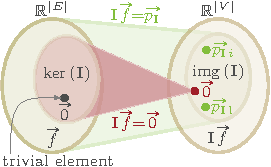
\includegraphics[scale=1,page=1]{networkAnalyzes/figures/ImageAndKernelOfALinearMappingIncidenceMatrix.pdf}
    % 
    \vspace{-5mm}%
    \caption[The image and kernel of the incidence
    matrix~\glssymbol{incidenceMatrix}.]{%
    % 
    The image~$\fimage{\glssymbol{incidenceMatrix}}$ and kernel~$\fkernel{
    \glssymbol{incidenceMatrix}}$ of the incidence
    matrix~\glssymbol{incidenceMatrix} for the linear map~$
        % 
        \glssymbol{incidenceMatrix}
        \colon
        \reals^{
            \fmagnitude{\glssymbol{edges}}
        }
        \to
        \reals^{
            \fmagnitude{\glssymbol{vertices}}
        }
        % 
    $.
    %
    }%
    % 
    \label{ch:network-analysis:fig:kernel-and-image-incidenceMatrix}%
    \vspace{-2mm}%
    % 
\end{wrapfigure}%
% 
\noindent Note that a \emph{trivial element} of the kernel is the neutral
element, \ie, in the vector space this is the zero vector~$\vv{0}$
(see~\cref{ch:network-analysis:fig:kernel-and-image-incidenceMatrix} left side).
If the kernel consists of the neutral element only then the linear map is
injective.
% 
% The dimension or size of the kernel, thus, describes the degree by which we
% fail the injectivity.
% 
From~\textcite[p.66; Theorem 4--3]{Ses61}, we know that the rank of the
matrix~\glssymbol{incidenceMatrix} is~$
% 
\rankx{ \glssymbol{incidenceMatrix} }
=
\fmagnitude{ \glssymbol{vertices} } 
- 
k
% 
$ with~$k$ being the number of connected components.
% 
The idea is that summing up the rows leads to one row of zeros per connected
component, since every column of the incidence
matrix~\glssymbol{incidenceMatrix}---representing an edge---consists of exactly
one~$1$ entry and one~$-1$ entry, which gives us~$
    % 
    \rankx{\glssymbol{incidenceMatrix}} 
    \leq 
    \fmagnitude{ \glssymbol{vertices} }
    - k
    % 
$
(see~\cref{ch:network-analyzes:sec:mathematical-model:fig:TUM-proof}\screen{b}
on Page~\pageref{ch:network-analyzes:sec:mathematical-model:fig:TUM-proof} as 
example). The aforementioned structure of the incidence
matrix~\glssymbol{incidenceMatrix} leads to an upper triangle matrix for each
connected component that cannot be reduced further leading to~$
    % 
    \rankx{\glssymbol{incidenceMatrix}} 
    \geq 
    \fmagnitude{ \glssymbol{vertices} } 
    - k
    % 
$ and thus, $
    % 
    \rankx{\glssymbol{incidenceMatrix}} 
    = 
    \fmagnitude{ \glssymbol{vertices} } 
    - k
    % 
$.
% 
Recall that the rank of the incidence matrix~\glssymbol{incidenceMatrix} (\ie,
$\rankx{\glssymbol{incidenceMatrix}}$) corresponds to the number of edges in a
spanning forest. To determine the nullity~$
    % 
    \nullityx{\glssymbol{incidenceMatrix}} 
    \coloneqq 
    \dimensionx{\fkernel{\glssymbol{incidenceMatrix}}}
    % 
$ of the incidence matrix~\glssymbol{incidenceMatrix}, we introduce
the~\emph{rank-nullity theorem}.
% 
\begin{theorem}[Rank-nullity Theorem]
    For any matrix~$\constraintmatrix\in\reals^{r\times c}$ with~$r$ rows
    and~$c$ columns the rank~$\rank(\constraintmatrix)$ and
    nullity~$\nullity(\constraintmatrix)$ sum up to the number of columns.
    % 
    $$
        \rankx{\constraintmatrix} 
        + 
        \nullityx{\constraintmatrix} 
        = 
        c.
    $$
    % 
    The generalization to linear maps~$
        % 
        \constraintmatrix
        \colon 
        \reals^{ \fmagnitude{C} } 
        \to
        \reals^{ \fmagnitude{R} }
        % 
    $ is given by
    % 
    $$
        \dimensionx{\fimage{\constraintmatrix}} 
        + 
        \dimensionx{\fkernel{\constraintmatrix}} 
        =
        \dimensionx{ \reals^{ \fmagnitude{C} } }
        =
        \fmagnitude{C}.
    $$
    % 
    \label{ch:network-analysis:def:rank-nullity-theorem}
    % 
\end{theorem}
%
The incidence matrix~\glssymbol{incidenceMatrix} can be viewed as a linear map~$
    % 
    \glssymbol{incidenceMatrix}
    \colon
    \reals^{
        \fmagnitude{
            \glssymbol{edges}
        }
    }
    \to
    \reals^{
        \fmagnitude{
            \glssymbol{vertices}
        }
    }
    % 
$ with $
    % 
    \vv{\glssymbol{flow}}
    \mapsto
    \glssymbol{incidenceMatrix}
    \cdot
    \vv{\glssymbol{flow}}
    % 
$. The kernel~$\fkernel{\glssymbol{incidenceMatrix}}$ and
image~$\fimage{\glssymbol{incidenceMatrix}}$ of the incidence
matrix~\glssymbol{incidenceMatrix} are given
in~\cref{ch:network-analysis:eq:incidence-matrix-image-and-kernel}.
% 
\begin{subequations}% 
\begin{align}%
    % 
    \fkernel{\glssymbol{incidenceMatrix}}
    &
    \coloneqq 
    \{
        \vv{\glssymbol{flow}}
        \in
        \reals^{\fmagnitude{\glssymbol{edges}}}
        \mid 
        \glssymbol{incidenceMatrix}
        \cdot
        \vv{\glssymbol{flow}} 
        = 
        \vv{0}
    \} 
    &
    \subseteq
    \reals^{\fmagnitude{\glssymbol{edges}}}
    % 
    \label{ch:network-analysis:eq:incidence-matrix-kernel}
    % 
    \\
    % 
    \fimage{\glssymbol{incidenceMatrix}}
    &
    \coloneqq 
    \{
        \frighthandsidevector{\glssymbol{incidenceMatrix}}
        \in
        \reals^{\fmagnitude{\glssymbol{vertices}}}
        \mid 
        \exists
        \vv{\glssymbol{flow}}
        \in
        \reals^{\fmagnitude{\glssymbol{edges}}}
        \colon 
        \glssymbol{incidenceMatrix}
        \cdot
        \vv{\glssymbol{flow}} 
        = 
        \frighthandsidevector{\glssymbol{incidenceMatrix}}
    \} 
    &
    \subseteq
    \reals^{\fmagnitude{\glssymbol{vertices}}}
    % 
    \label{ch:network-analysis:eq:incidence-matrix-image}
    % 
\end{align}%
\label{ch:network-analysis:eq:incidence-matrix-image-and-kernel}
% 
\end{subequations}% 
%
A kernel~$\fkernel{\glssymbol{incidenceMatrix}}$ of the incidence
matrix~\glssymbol{incidenceMatrix} is a set~$\fkernel{
\glssymbol{incidenceMatrix}}$ of vectors~$\vv{\glssymbol{flow}}$ such that the
homogeneous system~$
    % 
    \glssymbol{incidenceMatrix}
    \cdot
    \vv{ \glssymbol{flow} }
    = 
    \vv{0}
    % 
$ holds for all vectors in that set 
(see~\cref{ch:network-analysis:fig:kernel-and-image-incidenceMatrix} red area
and text). The image~$\fimage{\glssymbol{incidenceMatrix}}$ of the incidence
matrix are all vectors~$\frighthandsidevector{\glssymbol{incidenceMatrix}}$ for
which a solution exist 
(see~\cref{ch:network-analysis:fig:kernel-and-image-incidenceMatrix} green area
and text).
 
Using the rank-nullity theorem 
(see~\cref{ch:network-analysis:def:rank-nullity-theorem}) we get the dimension
of the kernel (\ie, the nullity when talking about matrices)
of~$
    % 
    \dimensionx{\fkernel{\glssymbol{incidenceMatrix}}}
    =
    \dimensionx{\glssymbol{edges}}
    -
    \dimensionx{\fimage{\glssymbol{incidenceMatrix}}}
    =
    \fmagnitude{\glssymbol{edges}} 
    - 
    \fmagnitude{\glssymbol{vertices}} 
    + k
    % 
$ 
%
that corresponds to the number of chords (\ie, edges not on a spanning forest).
A common way to construct the incidence matrix~\glssymbol{incidenceMatrix}
(see~\cref{ch:foundations} on Page~\pageref{ch:foundations:incidence-matrix}) of
row size~$\fmagnitude{\glssymbol{vertices}} - k$ is to define one
vertex~$\vertexa\in\glssymbol{generators}$ per connected component as slack%

% 
\begin{wrapfigure}{l}{3.5cm}%
    % 
    % \vspace{-4mm}
    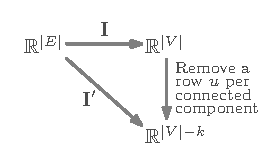
\includegraphics[scale=1,page=1]{networkAnalyzes/figures/NotesOnTheIncidenceProperty.pdf}
    % 
    % \vspace{-4mm}%
    \caption[Linear maps of the incidence matrix~\glssymbol{incidenceMatrix}.]{%
    Linear maps of the incidence matrix~\glssymbol{incidenceMatrix}
    and~$\glssymbol{incidenceMatrix}'$, where~$k$ is the number of connected
    components.
    %
    }%
    % 
    \label{ch:network-analysis:fig:mapping-incidenceMatrix}%
    % \vspace{-2mm}%
    % 
\end{wrapfigure}%
%
\noindent vertex and remove its row~$\vertexa$ (see
example~\cref{ch:network-analyzes:sec:mathematical-model:fig:TUM-proof}
\screen{b} on Page~\pageref{ch:network-analyzes:sec:mathematical-model:fig:TUM-proof},
where we remove vertex~$3$). From the property of the incidence
matrix~\glssymbol{incidenceMatrix} we know that every square submatrix
of~\glssymbol{incidenceMatrix} has a determinant that is either~$-1$, $0$,
or~$1$. Since every square non-singular submatrix of the incidence
matrix~\glssymbol{incidenceMatrix} of
size~$(\fmagnitude{\glssymbol{vertices}}-k)\times(\fmagnitude{
\glssymbol{vertices}}-k)$ that is the maximum square submatrix that constitutes
a spanning tree is unimodular (\ie, the determinant takes~$\pm 1$ values only)
and all determinants are either~$0, 1$, or~$-1$, the incidence
matrix~\glssymbol{incidenceMatrix} is \acrlong{tum} (in short~\gls{tum}).

\noindent If not noted otherwise, if we speak from now on of the incidence
matrix~\glssymbol{incidenceMatrix}, we mean the reduced incidence matrix that
has~$\fmagnitude{\glssymbol{vertices}}-k$ rows and thus, is defined by~$
    % 
    \glssymbol{incidenceMatrix}
    \in
    \{-1,0,1\}^{
        (
            \fmagnitude{\glssymbol{vertices}}-k
        )
        \times
        \fmagnitude{\glssymbol{edges}}
    }
    % 
$ (see~\cref{ch:network-analysis:fig:mapping-incidenceMatrix}).
% 
% 
%%%%%%%%%%%%%%%%%%%%%%%%%%%%%%%%%%%%%%%%%%%%%%%%%%%%%%%%%%%%%%%%%%%%%%%%%%%%%%%%
\paragraph{Feasible Flows and Thermal Line Limit}
\label{ch:network-analyzes:sec:mathematical-model:paragraph:capacity}
%%%%%%%%%%%%%%%%%%%%%%%%%%%%%%%%%%%%%%%%%%%%%%%%%%%%%%%%%%%%%%%%%%%%%%%%%%%%%%%%
% 
As already mentioned each edge has a natural limit of flow it is able to carry.
This is usually modeled by the capacity constraint that basically models the
thermal line limit
(\cref{ch:network-analyzes:sec:mathematical-model:eq:capacity-constraint}).
%
\begin{align}
    % 
    \fmagnitude{\glssymbol{flow}(\vertexa,\vertexc)}
    \leq
    \glssymbol{capacity}(\vertexa,\vertexc)
    \qquad
    \forall(\vertexa,\vertexc)\in\glssymbol{edges}.
    % 
    \label{ch:network-analyzes:sec:mathematical-model:eq:capacity-constraint}
\end{align}
%
We denote a flow~\glssymbol{flow} complying with the capacity constraints
as~\emph{feasible flow}. A~\gls{kcl} flow (see~\gls{kcl} flow on
Page~\pageref{ch:network-analyzes:sec:mathematical-model:paragraph:kcl-flow})
complying with the capacity constraint is thus called a~\emph{feasible~\gls{kcl}
flow}.
% 
\paragraph{\acrlong{kvl} (\gls{kvl})}
\label{ch:network-analyzes:sec:mathematical-model:paragraph:kvl}
% 
Kirchhoff's second law is known as~\emph{\acrlong{kvl}} (\gls{kvl}) and
describes the voltage angles in a~\emph{cycle} (also known as \emph{mesh}). A
cycle is a path~$
    % 
    \glssymbol{path}(\source,\sink) 
    \coloneqq
    \big(
        (\source,\vertexa_1), 
        (\vertexa_1,\vertexa_2), 
        \dots,
        (\vertexa_i,\sink)
    \big)
    % 
$, where at least~$\source = \sink$, otherwise it would not be closed. Cycles
have by definition an even degree.
% 
% and~$\vertexa_1, \vertexa_2,$ $\dots,$ $\vertexa_i,
% \source$ are distinct. 
% 
The set~\glssymbol{cycles} of cycles includes all cycles of a
graph~\glssymbol{graph}, which can be exponentially many in general. Note that
we distinguish between cycles and \emph{circuits}. A circuit has a degree
of~$2$. Thus, circuits are the same as simple cycles.
\acrlong{kvl} states that the voltages in a cycle sum up to zero
(\cref{ch:network-analyzes:sec:mathematical-model:eq:kvl-matrix-writing}).
Recall from~\cref{ch:foundations:sec:power-flow-analyses:subsec:Lin-DC-Model}
that in~\gls{dc}~\gls{feas} the voltages are substituted by the voltage angle
differences~\gls{voltageangledifference} and the
resistances~$\glssymbol{resistance}$ by~$\nicefrac{1}{\glssymbol{susceptance}}$.
The~\gls{kvl}-like equation is given
by~$
    % 
    \sum_{(\vertexa,\vertexc)\in\glssymbol{cycles}}
    \glssymbol{susceptance}(\vertexa,\vertexc)
    \cdot
    \left(
        \glssymbol{voltageangle}(\vertexc) 
        -
        \glssymbol{voltageangle}(\vertexa) 
        -
        \glssymbol{voltageangleshift}(\vertexa,\vertexc)
    \right) 
    = 
    0
    % 
$. In this section, we assume that~$
    % 
    \glssymbol{voltageangleshift}(\vertexa,\vertexc) = 0
    % 
$, \ie, we assume that there are no phase transformers or~\gls{facts} (see the
discussion in~\cref{ch:foundations:sec:power-flow-analyses:subsec:AC-Model}). In
terms of linear algebra, we can rewrite the latter by using the circuit
matrix~\glssymbol{cycleMatrix} and the~$\vv{\glssymbol{voltageangledifference}}$
vector
(\cref{ch:network-analyzes:sec:mathematical-model:eq:kvl-matrix-writing}).
% 
The oriented circuit
matrix~$
    \glssymbol{cycleMatrix}
    \in
    \{-1,0,1\}^{
        \fmagnitude{\glssymbol{cycles}}
        \times
        \fmagnitude{\glssymbol{edges}}
    }
    % 
$ is a matrix, where each row~\cycle represents a
cycle~$\cycle\in\glssymbol{cycles}$ and a column~\edge represents an
edge~$\edge\in\glssymbol{edges}$. The entry of~\glssymbol{cycleMatrix} is
either~$1$ (respectively~$-1$) when an edge~$\edge$ is in cycle~$\cycle$ in
direction (respectively opposite) with some predefined direction %~$\mathcal D$
for each cycle~$\cycle\in\glssymbol{cycles}$, or~$0$ if the edge is not in the
cycle~$\cycle$. The~\gls{kvl} using the circuit matrix is defined
in~\cref{ch:network-analyzes:sec:mathematical-model:eq:kvl-matrix-writing}.
%
\begin{align}
    \glssymbol{cycleMatrix}\vv{\glssymbol{voltageangledifference}} = \vv{0}, 
    % 
    \label{ch:network-analyzes:sec:mathematical-model:eq:kvl-matrix-writing}
\end{align}
%
where~$\glssymbol{cycleMatrix}\in\{-1,0,1\}^{\fmagnitude{\glssymbol{cycles}}\times\fmagnitude{\glssymbol{edges}}}$~\parencite[p.91]{Ses61}
is the oriented circuit matrix (\eg,
see~\cref{ch:network-analyzes:sec:mathematical-model:fig:TUM-proof} a or b on
Page~\pageref{ch:network-analyzes:sec:mathematical-model:fig:TUM-proof}; bottom
partition), and~$\vv{
\glssymbol{voltageangledifference}}\in\reals^{\fmagnitude{
\glssymbol{edges}}}$
with~$\glssymbol{voltageangledifference}\coloneqq
(\glssymbol{voltageangle}(\vertexc) -
\glssymbol{voltageangle}(\vertexa))_{(\vertexa,\vertexc)\in\glssymbol{edges}}$
is a vector of voltage angle differences at an edge
with~$\vv{\glssymbol{voltageangledifference}}\in\fkernel{\glssymbol{cycleMatrix}}$,
and~$\vv{0}$ is the zero vector of size~$\fmagnitude{\glssymbol{cycles}}$. The
formulation
in~\cref{ch:network-analyzes:sec:mathematical-model:eq:kvl-matrix-writing}
represents a homogeneous equation and thus, has always the trivial
solution~$\vv{\glssymbol{voltageangledifference}} = \vv{0}$. 
% Recall that the set
% of cycles includes potentially exponential many cycles, since~$\sum_{\ell = 2}^
% {\fmagnitude{\glssymbol{edges}}} \binom{\fmagnitude{\glssymbol{edges}}}{\ell} = -
% \fmagnitude{\glssymbol{edges}} + 2^{\fmagnitude{\glssymbol{edges}}}-1$. 
% 
\paragraph{Properties of the Circuit Matrix}
\label{ch:network-analyzes:sec:mathematical-model:paragraph:circuit-matrix-properties}
% 
Recall that the set~\glssymbol{cycles} of cycles includes potentially
exponentially many cycles. However, it suffices to work with a base of the cycle
space~\parencite[pp.498ff.]{Kir47} and thus, the circuit
matrix~\glssymbol{cycleMatrix} will only incorporate a fundamental cycle base in
this work. 

If we speak of the circuit matrix~\glssymbol{cycleMatrix} and we did not mention
anything else, we speak of the circuit matrix that only has fundamental cycles
as row vectors.
% 
\begin{definition}[Base]
    % 
    A~\emph{base} in a vector space is a maximum independent set of vectors that
    suffice to span the vector space.
    % 
    \label{ch:network-analyzes:sec:mathematical-model:def:base}
    % 
\end{definition}
% 
In general there are multiple bases that span the same vector space, which we
will see soon. Note that all bases have the same size~\parencite[p.514;
Theorem~6]{Whi35}.
% 
% A simple cycle is a minimal dependent set that contributes at least one edge
% to a base~\parencite[p.511; Theorem 2]{Whi35}. This means that a simple cycle is
% not in a base, since a base represents the maximum independent set.
% 
\begin{definition}[Fundamental Cycle Base]
    % 
    Let~$
        % 
        \glssymbol{graph} = ( \glssymbol{vertices}, \glssymbol{edges} )
        % 
    $ be a graph, let~$
        % 
        \tree = ( \glssymbol{vertices}, \glssymbol{edges} )
        % 
    $ be a spanning forest, and let~$
        % 
        \glssymbol{edges}_{\mathrm{chords}}
        \coloneqq
        \glssymbol{edges}(\glssymbol{graph})
        \setminus
        \glssymbol{edges}(\tree)
        % 
    $ be a set of chords. A walk from one endpoint~\vertexa of the
    chord~$(\vertexa, \vertexc)$ to the other endpoint~\vertexc using the
    spanning forest branches~$\glssymbol{edges}(\tree)$ defines a cycle that
    differs from the other cycles in~$\glssymbol{cycleMatrix}$ by at least the
    chord edge~$(\vertexa,\vertexc)$. 
    % 
    A \emph{fundamental cycle base} is defined by a spanning forest (by a
    spanning tree if the graph is connected), and a cycle in that base is
    defined by a chord (\ie, non-tree edge). 
    % 
    % A \emph{fundamental cycle base} is a set of chords (\ie, non-tree edge) that
    % can be constructed from a spanning tree~$\tree$. \franzi{Todo}
    % 
    \label{ch:network-analyzes:sec:mathematical-model:def:fundamental-cycle}
    % 
\end{definition}
% 
Note that a spanning forest has~$
    % 
    \fmagnitude{\glssymbol{vertices}} - k
    % 
$ edges---also denoted as tree branches---and~$
    % 
    \fmagnitude{\glssymbol{edges}} 
    -
    \fmagnitude{\glssymbol{vertices}} 
    + k
    % 
$ chords, where~$k$ is the number of connected components. The rank of the
circuit matrix is~$
    % 
    \rankx{\glssymbol{cycleMatrix}} 
    = 
    \fmagnitude{\glssymbol{edges}} 
    -
    \fmagnitude{\glssymbol{vertices}} 
    + k
    % 
$~\parencite[p.66;Theorem 4-5]{Ses61} and
the nullity is~$
    % 
    \nullityx{\glssymbol{cycleMatrix}} 
    = 
    \fmagnitude{\glssymbol{vertices}}
    - k
    % 
$~\parencite[p.64;Corollary 4-4]{Ses61}. In general, the circuit
matrix~\glssymbol{cycleMatrix} does not have a determinant of~$\pm
1$~\parencite{Oka55}\parencite[p.12; Lemma 3.3]{Kav09}. 

The circuit matrix~\glssymbol{cycleMatrix} is a linear map~$
    % 
    \glssymbol{cycleMatrix}
    \colon
    \reals^{
        \fmagnitude{
            \glssymbol{edges}
        }
    }
    \to
    \reals^{
        \fmagnitude{
            \glssymbol{cycles}
        }
    }
    % 
$ with~$
    % 
    \vv{
        \glssymbol{voltageangledifference}
    }
    \mapsto
    \glssymbol{cycleMatrix}
    \cdot    
    \vv{
        \glssymbol{voltageangledifference}
    }
    % 
$. The kernel~$\kernel(\glssymbol{cycleMatrix})$ and
image~$\image(\glssymbol{cycleMatrix})$ of the circuit
matrix~\glssymbol{cycleMatrix} are defined 
in~\cref{ch:network-analysis:eq:circuit-matrix-image-and-kernel} and
illustrated in~\cref{ch:network-analysis:fig:kernel-and-image-circuiteMatrix}
by the red or green area, respectively.
% 
\begin{subequations}
% 
\begin{align}
    % 
    \fkernel{
        \glssymbol{cycleMatrix}
    }
    &
    \coloneqq 
    \{
        \vv{
            \glssymbol{voltageangledifference}
        }
        \in
        \reals^{
            \fmagnitude{
                \glssymbol{edges}
            }
        }
        \mid 
        \glssymbol{cycleMatrix}
        \cdot
        \vv{\glssymbol{voltageangledifference}} 
        = 
        \vv{0}
    \} 
    &
    \subseteq
    \reals^{
        \fmagnitude{
            \glssymbol{edges}
        }
    }
    % 
    \label{ch:network-analysis:eq:circuit-matrix-kernel}
    % 
    \\
    % 
    \fimage{
        \glssymbol{cycleMatrix}
    }
    &
    \coloneqq 
    \{
        \frighthandsidevector{\glssymbol{cycleMatrix}}
        \in
        \reals^{
            \fmagnitude{
                \glssymbol{cycles}
            }
        }
        \mid 
        \exists
        \vv{
            \glssymbol{voltageangledifference}
        }
        \in
        \reals^{
            \fmagnitude{
                \glssymbol{edges}
            }
        }
        \colon 
        \glssymbol{cycleMatrix}
        \cdot
        \vv{
            \glssymbol{voltageangledifference}
        } 
        = 
        \frighthandsidevector{\glssymbol{cycleMatrix}}
    \} 
    &
    \subseteq 
    \reals^{
        \fmagnitude{
            \glssymbol{cycles}
        }
    }
    % 
    \label{ch:network-analysis:eq:circuit-matrix-image}
    % 
\end{align}
\label{ch:network-analysis:eq:circuit-matrix-image-and-kernel}
\end{subequations}
% 
A kernel~$\fkernel{\glssymbol{cycleMatrix}}$ of the circuit
matrix~$\glssymbol{cycleMatrix}$ is a set~$\fkernel{\glssymbol{cycleMatrix}}$ of
vectors~$\vv{\glssymbol{voltageangledifference}}$ such that the%

\begin{wrapfigure}{l}{4.5cm}%
    % 
    % \vspace{-4mm}
    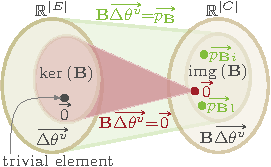
\includegraphics[scale=1,page=1]{networkAnalyzes/figures/ImageAndKernelOfALinearMapping.pdf}
    % 
    \vspace{-5mm}%
    \caption[The image and kernel of the circuit
    matrix~\glssymbol{cycleMatrix}.]{%
    % 
    The image~$\fimage{\glssymbol{cycleMatrix}}$ and kernel~$\fkernel{
    \glssymbol{cycleMatrix}}$ of the circuit matrix~\glssymbol{cycleMatrix} for
    the linear map~$
        % 
        \glssymbol{cycleMatrix}
        \colon
        \reals^{
            \fmagnitude{\glssymbol{edges}}
        }
        \to
        \reals^{
            \fmagnitude{\glssymbol{cycles}}
        }
        % 
    $.
    %
    }%
    % 
    \label{ch:network-analysis:fig:kernel-and-image-circuiteMatrix}%
    \vspace{-2mm}%
    % 
\end{wrapfigure}%
% 
\noindent homogeneous system~$
    % 
    \glssymbol{cycleMatrix}
    \cdot
    \vv{\glssymbol{voltageangledifference}} 
    =
    \vv{0}
    % 
$ holds for all vectors in that set
(see~\cref{ch:network-analysis:fig:kernel-and-image-circuiteMatrix} red area and
text). The image~$\fimage{
\glssymbol{cycleMatrix}}$ of the circuit matrix are all vectors~$
\frighthandsidevector{\glssymbol{cycleMatrix}}$ for which a solution exist 
(see~\cref{ch:network-analysis:fig:kernel-and-image-circuiteMatrix} green area
and text).

% , but a determinant
% of~$\pm 2^i$ with~$i\in\naturals$ and~$i$ being fix for a circuit
% matrix~\glssymbol{cycleMatrix}~\parencite{Oka55}. 
\noindent Using the rank-nullity theorem
(see~\cref{ch:network-analysis:def:rank-nullity-theorem}) 
we get the dimension of the kernel (nullity when talking about matrices) 
of~$
    % 
    \dimensionx{\fkernel{\glssymbol{cycleMatrix}}}
    =
    \dimensionx{\glssymbol{edges}}
    -
    \dimensionx{\fimage{\glssymbol{cycleMatrix}}}
    =
    \fmagnitude{\glssymbol{edges}} 
    - 
    \fmagnitude{\glssymbol{edges}} 
    +
    \fmagnitude{\glssymbol{vertices}} 
    - k
    =
    \fmagnitude{\glssymbol{vertices}} 
    - k
    % 
$.
 
\noindent However, \textcite{Ced55} showed that for a fundamental system of
circuits---that is used in our case---the determinant can only take values
of~$-1$, $0$, or $1$ for every square submatrix and~$\pm 1$ for a set of chords
that represents a maximal square matrix
(see~\cref{ch:network-analyzes:sec:mathematical-model:fig:TUM-proof}\screen{a}
or~\screen{b} bottom right partition). As for the incidence
matrix~\glssymbol{incidenceMatrix} above this means that the
matrix~\glssymbol{cycleMatrix} is~\gls{tum}.
% 
\begin{lemma}[\gls{tum} bases]
    The incidence matrix~\glssymbol{incidenceMatrix} and the
    circuit matrix~\glssymbol{cycleMatrix} are~\gls{tum} bases.
    % 
    \label{ch:network-analyzes:sec:mathematical-model:lem:I-and-B-TUM-sep}
\end{lemma}
%
\paragraph{Relationship between Incidence and Circuit Matrix}
\label{ch:network-analyzes:sec:mathematical-model:paragraph:relationsship-i-c-m}
% 
We get the relationship between the incidence matrix~\glssymbol{incidenceMatrix}
and the circuit matrix~\glssymbol{cycleMatrix}
in~\cref{ch:network-analyzes:sec:mathematical-model:eq:AB-orthogonality}.
% 
\begin{align}
    \glssymbol{incidenceMatrix}
    \transpose{\glssymbol{cycleMatrix}} 
    = 
    \mathbf{0}
    \quad
    % 
    \text{and}
    % 
    \quad
    \glssymbol{cycleMatrix}
    \transpose{\glssymbol{incidenceMatrix}} 
    = 
    \mathbf{0},
    % 
    \label{ch:network-analyzes:sec:mathematical-model:eq:AB-orthogonality}
\end{align}
% 
where~$\mathbf{0}$ is a matrix with zeros only of
dimension~$\fmagnitude{\glssymbol{vertices}}\times\fmagnitude{\glssymbol{cycles}}$
(respectively~$\fmagnitude{\glssymbol{cycles}}\times\fmagnitude{\glssymbol{vertices}}$).
Thus, the incidence matrix~\glssymbol{incidenceMatrix} is orthogonal to the
circuit matrix~\glssymbol{cycleMatrix}. One way to prove that is given
by~\textcite[p.66; Theorem 4-6]{Ses61} that uses the property of circuits that
have a degree of~$\degree(\vertexa) = 2$ at all
vertices~$\vertexa\in\glssymbol{vertices}$.
% 
Again note that both matrices~\glssymbol{incidenceMatrix}
and~\glssymbol{cycleMatrix} are orthogonal to each other (\ie, every vector
of~\glssymbol{incidenceMatrix} is orthogonal to every vector
in~\glssymbol{cycleMatrix}). Note that this also means that the vectors are
linear independent to each other. By doing a vertex transformation, we are able
to describe the voltage angle difference~$\glssymbol{voltageangledifference}
(\vertexa,\vertexc)$ vector by voltage angles~$\glssymbol{voltageangle}
(\vertexa)$ and~$\glssymbol{voltageangle}(\vertexc)$ for all
edges~$(\vertexa,\vertexc)\in\glssymbol{edges}$. However, this simple
transformation is based on the connection
that~$
    % 
    \glssymbol{cycleMatrix}
    \vv{\glssymbol{voltageangledifference}} 
    = 
    \vv{0}
    % 
$ and based on the relationship shown
in~\cref{ch:network-analyzes:sec:mathematical-model:eq:AB-orthogonality}.
% 
The connection given
in~\cref{ch:network-analyzes:sec:mathematical-model:eq:AB-orthogonality} allows
us to describe~$\vv{\glssymbol{voltageangledifference}}$ by the
linear combination of the tree branches~$
    % 
    \vv{\glssymbol{voltageangledifference}} 
    =
    \transpose{\glssymbol{incidenceMatrix}}
    \vv{\glssymbol{voltageangle}}
    % 
$ for each connected component (compare
also~\cref{ch:foundations:sec:power-flow-analyses:eq:assumption:vm:1,ch:network-analyzes:sec:mathematical-model:eq:kvl-ohm-function-writing}),
where~$
    % 
    \vv{\glssymbol{voltageangle}}
    \in 
    \reals^{\fmagnitude{\glssymbol{vertices}}-k}
    % 
$ with~$k$ representing the number of connected components~\parencite[Theorem
6-6, p. 123]{Ses61}. This means, we can find~$
    % 
    \glssymbol{cycleMatrix}
    \vv{\glssymbol{voltageangledifference}} 
    = 
    \vv{0}
    % 
$, which is equivalent of finding a~$
    % 
    \glssymbol{cycleMatrix}
    \transpose{\glssymbol{incidenceMatrix}}
    \vv{\glssymbol{voltageangle}} 
    = 
    \vv{0}
    % 
$. Since we know
from~\cref{ch:network-analyzes:sec:mathematical-model:eq:AB-orthogonality}
that~$
    % 
    \glssymbol{cycleMatrix}
    \transpose{\glssymbol{incidenceMatrix}} 
    =
    \mathbf{0}
    % 
$ this equation holds independent of the voltage angle
vector~$\vv{\glssymbol{voltageangle}}$. In addition, we would like to know when
there is a~$
    % 
    \vv{\glssymbol{voltageangle}}
    \in
    \reals^{
        \fmagnitude{\glssymbol{vertices}}
    }
    % 
$ such that~$
    % 
    \vv{\glssymbol{voltageangledifference}} 
    = 
    \transpose{
        \glssymbol{incidenceMatrix}
    }
    % \cdot
    \vv{\glssymbol{voltageangle}}
    % 
$. The latter is equivalent to the question of when~$
    % 
    \vv{\glssymbol{voltageangledifference}}
    \in
    \fimage{
        \transpose{\glssymbol{incidenceMatrix}}
    }
    % 
$. We have to show when~$
    % 
    \fkernel{\glssymbol{cycleMatrix}}
    \subseteq
    \fimage{\transpose{\glssymbol{incidenceMatrix}}}
$. This is the case when we chose the same spanning tree to construct both
matrices. Note that it suffices to compute the voltage angle differences along
a spanning tree, since the others result from these voltage angles.
% 
\paragraph{\gls{kvl} Flow}
\label{ch:network-analyzes:sec:mathematical-model:paragraph:kvl-flow}
% 
Applying the latter to Ohm's law gives us the typical equation
known from literature
(\cref{ch:network-analyzes:sec:mathematical-model:eq:kvl-ohm-function-writing}).
%
\begin{align}
    \glssymbol{susceptance}(\vertexa,\vertexc)
    \cdot
    \big(\glssymbol{voltageangle}(\vertexc)
    -
    \glssymbol{voltageangle}(\vertexa)
    \big) = \glssymbol{flow}(\vertexa,\vertexc).
    % 
    \label{ch:network-analyzes:sec:mathematical-model:eq:kvl-ohm-function-writing}
\end{align}
%
A flow~\glssymbol{flow} complying
with~\cref{ch:network-analyzes:sec:mathematical-model:eq:kvl-ohm-function-writing}
is called~\emph{\gls{kvl} flow} and if it complies with the capacity constraint
it is called~\emph{feasible~\gls{kvl} flow}. 

Using the aforementioned relationship
(\cref{ch:network-analyzes:sec:mathematical-model:eq:kvl-ohm-function-writing}),
we can
reformulate~\cref{ch:network-analyzes:sec:mathematical-model:eq:kvl-matrix-writing}
such that we replace voltage angle
differences~$\vv{\glssymbol{voltageangledifference}}$ by
flows~$\vv{\glssymbol{flow}}$. Note that~$
    % 
    \glssymbol{susceptance}(\vertexa,\vertexc)
    = 
    \nicefrac{ 1 }{ \glssymbol{reactance}(\vertexa,\vertexc) }
    % 
$ and that~\textquote{$\circ$} is the Schur product (or entrywise product). 
% 
\begin{subequations}
% 
\begin{align}
    % 
    \vv{\glssymbol{flow}} 
    = 
    \vv{\glssymbol{susceptance}} 
    \circ 
    \vv{\glssymbol{voltageangledifference}} 
    % 
    &\Leftrightarrow
    % 
    \hspace{2.35mm}
    \vv{\glssymbol{voltageangledifference}} 
    = 
    \vv{\glssymbol{reactance}} 
    \circ 
    \vv{\glssymbol{flow}} 
    \\
    \glssymbol{cycleMatrix}
    \vv{\glssymbol{voltageangledifference}} 
    = 
    \vv{0}\hspace{10mm}
    % 
    &\Leftrightarrow
    % 
        \underbrace{
            \left(
                \glssymbol{cycleMatrix}
                \circ    
                    (
                        \mathbb{1}^{ 
                            \fmagnitude{\glssymbol{edges}} 
                            \times 
                            1 
                        }
                        \cdot
                        \transpose{ \vv{\glssymbol{reactance}} }
                    )
            \right)
        }_{
            \eqqcolon
            \glssymbol{cycleMatrix}'
        }
    \cdot
    \vv{\glssymbol{flow}} 
    = 
    \vv{0}
    % 
    \label{ch:network-analyzes:sec:mathematical-model:eq:voltage-angle-diff-replacement-to-flows}
    % 
\end{align}
\label{ch:network-analyzes:sec:mathematical-model:eq:voltage-angle-diff-replacement-to-flows:allg}
\end{subequations}
% 
Since~$\vv{\glssymbol{reactance}}$ is a vector of constant values, we just
multiply the entries in the circuit matrix~$\glssymbol{cycleMatrix}$ by~$\vv{
\glssymbol{reactance}}$ resulting in a new circuit matrix~$
\glssymbol{cycleMatrix}'$, which results in~\cref{ch:network-analyzes:sec:mathematical-model:eq:voltage-angle-diff-replacement-to-flows:main}.
% 
\begin{align}
    \glssymbol{cycleMatrix}'
    \cdot
    \vv{\glssymbol{flow}}
    =
    \vv{0}
    % 
    \label{ch:network-analyzes:sec:mathematical-model:eq:voltage-angle-diff-replacement-to-flows:main}
    % 
\end{align}
% 
% 
\paragraph{Feasible Electrical Flow}
\label{ch:network-analyzes:sec:mathematical-model:paragraph:feasible-electrical-flow}
% 
In the following, we define feasible electrical flows that represent solutions
to~\gls{dc}~\gls{feas}.
% 
\begin{definition}[Feasible Electrical Flow]
    A~\gls{kvl} flow that is also a~\gls{kcl} flow is called~\emph{electrical
    flow} and if it complies to the capacity constraint, too, it is
    called a~\emph{feasible electrical flow}.
    % 
    \label{ch:network-analyzes:sec:mathematical-model:def:kvl-kcl-feasible-flow}
\end{definition}
% 
\gls{dc}~\gls{feas} and~\gls{dc}~\gls{mpfp} constitute a system of linear
equations and an~\gls{lp}, respectively. In the following, we summarize the
problem definitions of~\gls{dc}~\gls{feas} and~\gls{mpfp}.
% 
\begingroup
    %%%%%%%%%%%%%%%%%%%%%%%%%%%%%%%%%%% Problem %%%%%%%%%%%%%%%%%%%%%%%%%%%%%%%%%%%%
\begin{problem}[framed]{\acrlong{dc} \acrlong{feas} \gls{dc}-\gls{feas}$
(\glssymbol{network})$}%
  Instance: & An exact bounded network~\dcnetworktuple, \ie,
  $
  % \forall\vertex\in\glssymbol{generators}
  % \colon
  \glssymbol{realpowergeneration}
  \equiv
  \glssymbol{realpowergenerationmin}
  \equiv
  \glssymbol{realpowergenerationmax}$
  and~$
  % \forall
  % \vertex\in\glssymbol{consumers}
  % \colon
  \glssymbol{realpowerdemand}
  \equiv
  \glssymbol{realpowerdemandmin}
  \equiv
  \glssymbol{realpowerdemandmax}
  % 
  $.
  \\
  % 
  Question: & Is there a feasible electrical flow~\glssymbol{flow}
  (see~\cref{ch:network-analyzes:sec:mathematical-model:eq:kcl-matrix-writing,ch:network-analyzes:sec:mathematical-model:eq:kvl-matrix-writing,ch:network-analyzes:sec:mathematical-model:eq:capacity-constraint})?
  % ch:network-analyzes:sec:mathematical-model:eq:kvl-ohm-function-writing
\end{problem}%
    \label{ch:networkAnalysis:problems:DC_FEAS_Exact-Decision_Problem}
\endgroup
% 
A feasible electrical flow that maximizes the flow value~$
\glssymbol{flowvalue}(\glssymbol{network},\glssymbol{flow})
\coloneqq 
\sum_{\vertexa\in\glssymbol{generators}}
\glssymbol{netflow}(\vertexa)
$
is called~$\gls{mpfp}(\glssymbol{network})$ and its value is denoted
by~$\opt_{\gls{mpfp}}(\glssymbol{network})$. The optimization problem is stated
in the following.
%
\begingroup
    %%%%%%%%%%%%%%%%%%%%%%%%%%%%%%%%%%% Problem %%%%%%%%%%%%%%%%%%%%%%%%%%%%%%%%%%%%
\begin{problem}[framed]{\acrlong{dc} \acrlong{mpfp}~\gls{dc}-\gls{mpfp}%
$(\glssymbol{network})$}%
  Instance: & A network~\dcnetworktuple.\\
  % 
  Objective: & Find a feasible electrical flow~\glssymbol{flow}
  (see~\cref{ch:network-analyzes:sec:mathematical-model:eq:kcl-matrix-writing,ch:network-analyzes:sec:mathematical-model:eq:kvl-matrix-writing,ch:network-analyzes:sec:mathematical-model:eq:capacity-constraint}) 
  % ch:network-analyzes:sec:mathematical-model:eq:kvl-ohm-function-writing
  such that the flow value~$\glssymbol{flowvalue}(\glssymbol{network})$ is
  maximum among all choices of~\glssymbol{flow}.
\end{problem}%
    \label{ch:networkAnalysis:problems:DC_MPF-Decision_Problem}
\endgroup
%
\paragraph{Algorithms to Solve~DC~FEAS}%
\label{ch:network-analyzes:sec:mathematical-model:paragraph:algos-dc-feas}%
% 
Possibilities to get a feasible power flow are to formulate the system of linear
equations or~\gls{lp} and run it using a solver such as
Gurobi~\parencite{gurobi}, or to apply the following algorithm.
% 
\begin{lemma}[{{\textcite[p.36; Lemma 1]{Sha87}}}]
    Let every edge of~\glssymbol{graph} have a resistance~$\resistance\equiv 1$.
    Let~$\tree$ denote the number of spanning trees and
    let~$
        % 
        \tree(\source,\vertexa\rightarrow\vertexc,\sink)
        % 
    $ be the number of spanning trees that contain the
    edge~$(\vertexa,\vertexc)$ in that particular direction meaning the spanning
    tree has a path from~\source to~\sink that visits vertex~\vertexa first and
    then vertex~\vertexc by using the edge~$
        % 
        (\vertexa,\vertexc)
        \in
        \glssymbol{edges}
        % 
    $. Let~$
        % 
        \glssymbol{realpowergeneration}
        \equiv
        \glssymbol{realpowerdemand}
        \equiv 
        1
        % 
    $ and let~$
        % 
        \glssymbol{flow}(\vertexa,\vertexc)
        =
        \nicefrac{
            \big(
                \tree(\source,\vertexa\rightarrow\vertexc,\sink)
                -
                \tree(\source,\vertexc\rightarrow\vertexa,\sink)
            \big)
        }{
            \tree
        } 
        % 
    $. Then~\glssymbol{flow} is a feasible electrical flow in~\glssymbol{graph}.
    % 
    % Then~$\glssymbol{flow}(\vertexa,\vertexc)$ is the flow on the edge~$
    % (\vertexa,\vertexc)\in\glssymbol{edges}$ oriented from~\vertexa to~\vertexc.
    % 
    \label{ch:network-analyzes:sec:mathematical-model:lem:current_edge_from_a_to_b}
    % 
\end{lemma}
% 
The generalization---where we have no unit resistances~\glssymbol{resistance}, 
but arbitrary ones---given by~\textcite[p.38]{Sha87} was already given
by~\textcite[pp.155ff.]{Ses61}. Instead of just using the number of spanning
trees, we calculate for each spanning tree the product of the admittances of the
branches of that spanning tree and sum over all spanning trees. The proof of the
lemma uses the Binet-Cauchy-Theorem~\parencite[p.32]{Ses61}. Note that a graph
can have exponentially many spanning trees and computing the flow for each edge
using this techniques is quite inefficient, but provides an exponential time
algorithm to compute the electrical flow of the power grid.
% 
%%%%%%%%%%%%%%%%%%%%%%%%%%%%%%%%%%%%%%%%%%%%%%%%%%%%%%%%%%%%%%%%%%%%%%%%%%%%%%%%
\subsection{Properties of Electrical Flows}%
\label{ch:network-analyzes:sec:mathematical-model:properties-elec-flows}%
%%%%%%%%%%%%%%%%%%%%%%%%%%%%%%%%%%%%%%%%%%%%%%%%%%%%%%%%%%%%%%%%%%%%%%%%%%%%%%%%
% 
Note that we use a base for the columns of the incidence and circuit matrix
denoted by~\glssymbol{incidenceMatrix} and~\glssymbol{cycleMatrix},
respectively, where all equations are linear independent. Since the whole system
of equations has full rank the solution to a feasible electrical flow is unique,
which we show in the following.
%
\begin{lemma}[Uniqueness of \gls{dc} Electrical Flows]
    % 
    There is a unique solution to~\gls{dc} electrical flows if we have exact
    bounds.
    % 
    % lower bounds for generation~$\realpowergenerationmin$ and
    % demand~$\realpowerdemandmin$ are unbounded, and if such a solution exists.
    % 
    \label{ch:network-analyzes:sec:mathematical-model:lem:unique-flow}
    % 
\end{lemma}
% 
\begin{proof}
%
Recall that the incidence matrix~\glssymbol{incidenceMatrix} with~$
    % 
    \glssymbol{incidenceMatrix} 
    \in
    \reals^{
    (\fmagnitude{\glssymbol{vertices}} 
    - k)
    \times
    \fmagnitude{\glssymbol{edges}}}
    % 
$ and the circuit matrix~\glssymbol{cycleMatrix} with~$
    % 
    \glssymbol{cycleMatrix}
    \in
    \reals^{
    ( \fmagnitude{\glssymbol{edges}} 
    - \fmagnitude{\glssymbol{vertices}} 
    + k)
    \times
    \fmagnitude{\glssymbol{edges}}}
    % 
$ are bases. Since both matrices are bases the vectors are linear independent
in each matrix (\ie, this is a property of a base shown
in~\cref{ch:network-analyzes:sec:mathematical-model:eq:kvl-matrix-writing,ch:network-analyzes:sec:mathematical-model:eq:kcl-matrix-writing:1}).
% 
We now define a matrix~\constraintmatrix by~$
    % 
    \constraintmatrix 
    \coloneqq
    \binom{
        \glssymbol{incidenceMatrix}
    }{
        \glssymbol{cycleMatrix}'
    }
    % 
$ with~$\glssymbol{cycleMatrix}'$ from~\cref{ch:network-analyzes:sec:mathematical-model:eq:voltage-angle-diff-replacement-to-flows:main},
where~$
    % 
    \constraintmatrix
    \in
    \reals^{\fmagnitude{\glssymbol{edges}}\times\fmagnitude{\glssymbol{edges}}}
    % 
$ can be generalized to a linear map~$
    % 
    \constraintmatrix
    \colon
    \reals^{ \fmagnitude{ \glssymbol{edges} } }%
    \to
    \reals^{ \fmagnitude{ \glssymbol{edges} } }%
    % 
$ with~$
    % 
    \vv{ \glssymbol{flow} }%
    \mapsto%
    \constraintmatrix%
    \cdot%
    \vv{\glssymbol{flow}}%
    % 
$. Thus, the system of equations is defined by~$
    % 
    \constraintmatrix
    \cdot
    \vv{\glssymbol{flow}} 
    = 
    \frighthandsidevector{\constraintmatrix} 
    \coloneqq 
    \binom{
        \frighthandsidevector{\glssymbol{incidenceMatrix}}
    }{
        \vv{0}
    }
    % 
$ with vector~$\vv{0}$ of size~$
% 
\fmagnitude{\glssymbol{cycles}}
% 
$.
% 
The kernel~$\fkernel{\constraintmatrix}$ and the
image~$\fimage{\constraintmatrix}$ of matrix~\constraintmatrix are defined
in~\cref{ch:network-analysis:eq:constraintmatrix-matrix-image-and-kernel}.
%
\begin{subequations}
% 
\begin{align}
    % 
    \fkernel{\constraintmatrix}
    &
    \coloneqq 
    \{
        \vv{\glssymbol{flow}}
        \in
        \reals^{\fmagnitude{\glssymbol{edges}}}
        \mid 
        \constraintmatrix
        \cdot
        \vv{\glssymbol{flow}} 
        = 
        \vv{0}
    \} 
    &
    \subseteq
    \reals^{\fmagnitude{\glssymbol{edges}}}
    % 
    \label{ch:network-analysis:eq:constraintmatrix-matrix-kernel}
    % 
    \\
    % 
    \fimage{\constraintmatrix}
    &
    \coloneqq 
    \{
        \frighthandsidevector{\constraintmatrix} 
        \in
        \reals^{\fmagnitude{\glssymbol{edges}}}
        \mid 
        \exists
        \vv{\glssymbol{flow}}
        \in
        \reals^{\fmagnitude{\glssymbol{edges}}}
        \colon 
        \constraintmatrix
        \cdot
        \vv{\glssymbol{flow}} 
        = 
        \frighthandsidevector{\constraintmatrix} 
    \} 
    &
    \subseteq
    \reals^{\fmagnitude{\glssymbol{edges}}}
    % 
    \label{ch:network-analysis:eq:constraintmatrix-matrix-image}
    % 
\end{align}
\label{ch:network-analysis:eq:constraintmatrix-matrix-image-and-kernel}
\end{subequations} 
% 
From~\cref{ch:network-analyzes:sec:mathematical-model:eq:AB-orthogonality}, we
know that~$
    % 
    \glssymbol{incidenceMatrix} 
    \transpose{\glssymbol{cycleMatrix}} 
    =
    \mathbf{0}
    $ and~$
    \glssymbol{cycleMatrix} 
    \transpose{\glssymbol{incidenceMatrix}}
    =
    \mathbf{0}
    % 
$, which means that the dimension of the image of~\constraintmatrix is the sum
of the dimension of the images of the incidence matrix~\glssymbol{incidenceMatrix}
and circuit matrix~\glssymbol{cycleMatrix} given by~$
    % 
    \dimensionx{\fimage{\constraintmatrix}} 
    = 
    \dimensionx{\fimage{\incidenceMatrix}} 
    +
    \dimensionx{\fimage{\cycleMatrix}}  
    =
    \fmagnitude{\glssymbol{vertices}} - k
    +
    \fmagnitude{\glssymbol{edges}} - \fmagnitude{\glssymbol{vertices}} + k
    =
    \fmagnitude{\glssymbol{edges}}
    % 
$.
Using the rank-nullity theorem
(see~\cref{ch:network-analysis:def:rank-nullity-theorem}), we know that the
dimension of the kernel is~$\dimensionx{\fkernel{\constraintmatrix } } = 0$. 
Thus, \constraintmatrix as linear map is injective.
% 
% Now
% we consider two cases:
% % 
% \begin{compactenum}
%     \item If~$
%         \frighthandsidevector{\constraintmatrix} 
%         \not\in
%         \fimage{\constraintmatrix}
%     $, then the system has no solution.
%     % 
%     \item If~$
%         \frighthandsidevector{\constraintmatrix} 
%         \in
%         \fimage{\constraintmatrix}
%     $ there are two cases
%         \begin{compactenum}
%             \item $\dimensionx{\fimage{\constraintmatrix}} 
%                     < 
%                     \dimensionx{\glssymbol{edges}},$
%             \item $\dimensionx{\fimage{\constraintmatrix}} 
%                     = 
%                     \dimensionx{\glssymbol{edges}}.$
%         \end{compactenum}
% \end{compactenum}
% 
The dimension of the image of~\constraintmatrix is~$\fmagnitude{\edges}$, which
means that the matrix has full rank. We conclude that the system has a unique
non-trivial solution (see~\cref{ch:network-analyzes:fig:polytope-simple-example}).
% 
\end{proof}
%
% 
\begin{wrapfigure}{l}{6.5cm}% 
    \vspace{-0.6cm}
    % 
    \resizebox{6.35cm}{!}{%
\begin{tikzpicture}
\usepgfplotslibrary{fillbetween}
\usetikzlibrary{patterns}
\usetikzlibrary{intersections}
% pure inductive load
\begin{axis}[
    width=8.5cm,
    height=6.115cm,
    axis x line=middle, % center
    axis y line=middle, %none
    axis on top,
    domain=-4:7,
    xticklabels={$-4$, $-3$, $-2$, $-1$, $0$, $1$, $2$, $3$, $4$}, %\empty,
    xtick={-4.0, -3.0, -2.0, -1.0, 0, 1.0, 2.0, 3.0, 4.0},
    yticklabels={$-3$, $-2$, $-1$, $0$, $1$, $2$, $3$}, %
    ytick={-3.0, -2.0, -1.0, 0, 1.0, 2.0, 3.0},
    x tick style={color=KITblack70, thick,line cap=round},
    y tick style={color=KITblack70, thick,line cap=round},
    minor y tick num=1,
    minor x tick num=1,
    samples=1001,
    xlabel={$x$},
    ylabel={$y$},
    legend pos=outer north east,
    xmin=-4.0-0.5,
    xmax=4.0+0.5,
    ymin=-3.0-0.5,
    ymax=3.0+0.5,
    axis line style={KITblack70, thick}, %line cap=round, 
    x tick label style={font=\color{KITblack70}},
    y tick label style={font=\color{KITblack70}},
every axis x label/.style={
    at={(ticklabel* cs:1.0)},
    anchor=west,
},
every axis y label/.style={
    at={(ticklabel* cs:0.98)},
    anchor=south,
},
    x label style={font=\color{KITblack70}},
    y label style={font=\color{KITblack70}},
    % set clip=false to avoid clipping of nodes
    clip=false,
]
%
% Gray vertical lines
% 
    \def \xMin {-5.0}
    \def \xMax {5.0}
    \def \yMin {-4.0}
    \def \yMax {4.0}
%
% y cut at one
%
    \def \yBounded {1}
    % 
    \addplot[name path=fctYmax, mark=none, draw=none, line cap=round] 
    coordinates {(\xMin, 3.0 ) (\xMax, 3.0 )};
    % 
    \addplot[name path=fctYmin, mark=none, draw=none, line cap=round] 
    coordinates {(\xMin, -3.0 ) (\xMax, -3.0 )};
    % 
    \addplot[name path=fctXmin, mark=none, draw=none, line cap=round] 
    coordinates {(-4.0, \yMin ) (-4.0, \yMax )};
    % 
    \addplot[name path=fctXmax, mark=none, draw=none, line cap=round] 
    coordinates {(4.0, \yMin ) (4.0, \yMax )};
    % 
%
% Functions Representing the Simple "Hyperplanes", i.e., Straights
%
    \def \fctRed { -1 * x + 3 }
    \def \fctBlue { 1 * x - 1 }
    \def \fctDarkGreen { 3/2 * x + 3 }
    \def \fctLightGreen { -1/2 * x - 2 }
    % 
    % \newcommand{\drawge}{-- (rel axis cs:1,0) -- (rel axis cs:1,1) -- (rel axis cs:0,1) \closedcycle}
    % \newcommand{\drawle}{-- (rel axis cs:1,1) -- (rel axis cs:1,0) -- (rel
    % axis cs:0.01,0) \closedcycle}
    % 
    \addplot [name path=fctRed, domain = -0.5:5.1, ultra thick, KITred70, line
    cap=round] 
    {\fctRed} node[above,right,pos=1.0] {$ y = -x + 3$}; 
    % 
    \addplot [name path=fctBlue, domain = -2.5:4.1, ultra thick, KITseablue70,
    line cap=round] 
    {\fctBlue} node[above,right,pos=1.0] {$ y = x - 1$}; 
    % 
    \addplot [name path=fctDarkGreen, domain = -4.1:0.5, ultra thick,
    KITgreen70, line cap=round, fill=black]
    {\fctDarkGreen} 
    node[above,right,pos=0.98] 
    {$y = \nicefrac{3}{2} x + 3$};
    % 
    \addplot [name path=fctLightGreen, domain = -5.0:3.1, ultra thick,
    KITcyanblue70, line cap=round] 
    {\fctLightGreen} 
    node[above,right,pos=1.0] 
    {$y = -\nicefrac{x}{2} - 2$};
    %
    \addplot [line width=1pt,fill=KITcyanblue70,draw=none,fill opacity=0.08] 
    fill between[
            of=fctLightGreen and fctYmax,
            soft clip={domain=-5:5},
    ];
    % \addplot [draw=none, fill=KITseablue70,fill
    % opacity=0.908, domain=-4.5:\xMax]{\fctLightGreen} \drawge; 
    % \addplot [draw=none, fill=KITgreen70,fill
    % opacity=0.908, domain=-4.4:\xMax]{\fctDarkGreen} \drawle;
    % \addplot [draw=none, fill=KITgreen70,fill
    % opacity=0.908, domain=-4:\xMax]{\fctDarkGreen} \drawle; 
    % \addplot [draw=none, pattern=north west lines, pattern color=blue!40, domain=-10:12]
    %          {-5+2*x} \drawge;
    % \addplot [draw=none, pattern=horizontal lines, pattern color=blue!40, domain=-10:10]
    %          {3/2+x/2} \drawle; 
    % 
    \addplot [line width=1pt,fill=KITseablue70,draw=none,fill opacity=0.08] 
    fill between[
            of=fctBlue and fctXmin,
            soft clip={domain=-5:5},
    ];
    % 
    \addplot [line width=1pt,fill=KITred70,draw=none,fill opacity=0.08] 
    fill between[
            of=fctRed and fctYmin,
            soft clip={domain=-5:5},
    ];
    % 
    \addplot [line width=1pt,fill=KITgreen70,draw=none,fill opacity=0.08] 
    fill between[
            of=fctDarkGreen and fctXmax,
            soft clip={domain=-5:5},
    ];
    % 
    % 
%
% Cut Area of the four functions
%
    \addplot [line width=1pt,fill=orange,draw=none,fill opacity=0.2] 
    coordinates{
        (0,3) 
        (2,1) 
        (-2/3,-5/3) 
        (-5/2,3/2*-5/2+3)
    } node[above,pos=0.3,orange] {$\polyhedron$};
    % 
    \addplot [line width=1pt,fill=KITlilac70,draw=KITlilac70,fill opacity=0.2] 
    (-2/3,-5/3) circle (1ex);%
    %
    \addplot[mark=none, KITpalegreen, dashed, line cap=round] 
    coordinates {(\xMin, \yBounded ) (4.0, \yBounded )}
    node[right,pos=1.0]{$y$ is fixed to~$1$};
%
\end{axis}
\end{tikzpicture}
}%
    % 
    % \vspace{-0.05cm}
    % 
    \caption[A simple polytope example.]{The \textcolor{orange!60}
    {Polytope~\polyhedron} constituted by~$
    % 
     \textcolor{KITgreen70}{y \leq \nicefrac{3}{2} x + 3}$,
    % 
    $\textcolor{KITseablue70}{y \geq x - 1}$, 
    % 
    $\textcolor{KITred70}{y \leq -x + 3}$, and~$
    % 
     \textcolor{KITcyanblue70}{y \geq -\nicefrac{x}{2} - 2}$. 
    % 
    If~$\textcolor{KITpalegreen70}{y = 1}$, we reduce the solution space
    to~$x\in[-\nicefrac{4}{3}, 2]$. However, if~$y = -\nicefrac{5}{3}$ the
    solution is unique~$x = -\nicefrac{2}{3}$. So a unique solution corresponds
    to one point~\tikzPolytopePoint.
    % 
    % 
    }%
    \vspace{-0.4cm}
    % 
    \label{ch:network-analyzes:fig:polytope-simple-example}%
\end{wrapfigure}%
%  
Note that the system has no non-trivial solution if the generations and demands
are exact and the capacities are chosen in such a way that these generations and
demands cannot be fulfilled. In the following, we extend the system by capacity
constraints discussed
in~\cref{ch:network-analyzes:sec:mathematical-model:eq:capacity-constraint}.% We ask if the system with the capacity constraints has still full rank.
% 

The capacity constraint can be reformulated in a matrix writing by~$
    % 
    {\mathbb 1}^{
        \fmagnitude{ \glssymbol{edges} } 
        \times
        \fmagnitude{ \glssymbol{edges} } 
    }
    \cdot
    \vv{\glssymbol{flow}}
    \leq
    \vv{\glssymbol{capacity}}
    % 
$, where~$
    % 
    {\mathbb 1}^{ 
        \fmagnitude{\glssymbol{edges} } 
        \times 
        \fmagnitude{\glssymbol{edges} } 
    }
    % 
$ is the identity matrix of size~$
    % 
    \fmagnitude{ \glssymbol{edges} }
    \times
    \fmagnitude{ \glssymbol{edges} }
    % 
$ and the vector of capacities is~$
    % 
    \vv{ \glssymbol{capacity} } 
    \in 
    \reals^{
        \fmagnitude{
            \glssymbol{edges}
        }
    }
    % 
$. With the capacity constraint we get a matrix~$
    % 
    \constraintmatrix' 
    = 
    \transpose{
    (
        \glssymbol{incidenceMatrix}, 
        \glssymbol{cycleMatrix}', 
        {\mathbb1}^{
            \fmagnitude{\glssymbol{edges} } 
            \times
            \fmagnitude{\glssymbol{edges} } 
        }
    )
    }
    % 
$ of size~$
    % 
    \constraintmatrix'
    \in
    \reals^{
        ( 2\fmagnitude{\glssymbol{edges}} )
        \times
        \fmagnitude{\glssymbol{edges}}
    } 
    % 
$ with~$\glssymbol{cycleMatrix}'$ 
from~\cref{ch:network-analyzes:sec:mathematical-model:eq:voltage-angle-diff-replacement-to-flows:main}.
Note that the additional submatrix has no influence on the dimension of the
image meaning~$
    % 
    \dimensionx{\fimage{\constraintmatrix'}} 
    = 
    \fmagnitude{\glssymbol{edges}}
    % 
$, \ie, using the rank-nullity-theorem
(\cref{ch:network-analysis:def:rank-nullity-theorem}), we get the dimension of
the kernel~$
    % 
    \dimensionx{\fkernel{\constraintmatrix}} = 0
    % 
$. The matrix remains to have a full rank, but we have inequality constraints.
With exact supplies (\ie, $
    % 
    \glssymbol{realpowergeneration}
    \equiv
    \glssymbol{realpowergenerationmin}
    \equiv
    \glssymbol{realpowergenerationmax}
    % 
$) and exact demands (\ie, $
    % 
    \glssymbol{realpowerdemand}
    \equiv
    \glssymbol{realpowerdemandmin}
    \equiv
    \glssymbol{realpowerdemandmax}
    % 
$) the capacity constraints have only influence on the feasibility of a
solution, since~$
    % 
    \constraintmatrix 
    \cdot 
    \vv{\glssymbol{flow}} 
    = 
    \frighthandsidevector{\constraintmatrix} 
    % 
$ gives us a unique solution the inequality~$
    % 
    \mathbb{1}^{ 
        \fmagnitude{\glssymbol{edges}} 
        \times 
        \fmagnitude{\glssymbol{edges}} 
    }
    \cdot
    \vv{\glssymbol{flow}}
    \leq
    \vv{\glssymbol{capacity}}
    % 
$ might lead to a polytope that does not include that solution.

If we apply upper bounds~$\frighthandsidevector{\constraintmatrix\uparrow}$
with~$
    % 
    \glssymbol{realpowergenerationmax}, 
    \glssymbol{realpowerdemandmax}
    \in
    \posreals
    % 
$, and lower bounds~$\frighthandsidevector{\constraintmatrix\downarrow}$ with~$
    % 
    \glssymbol{realpowergenerationmin}, 
    \glssymbol{realpowerdemandmin}
    \in
    \posreals
    % 
$ for the generations and demands, we get the following system of
inequalities.
% 
\begin{subequations}
\begin{align}
    % 
    \hphantom{-}\constraintmatrix
    \cdot
    \vv{\glssymbol{flow}} 
    % 
    &\leq
    % 
    \hphantom{-}\frighthandsidevector{\constraintmatrix\uparrow} 
    % 
    \label{ch:network-analysis:eq:upper-bounds}
    % 
    \\
    % 
    -\constraintmatrix
    \cdot
    \vv{\glssymbol{flow}} 
    % 
    &\leq
    % 
    -\frighthandsidevector{\constraintmatrix\downarrow} 
    % 
    \label{ch:network-analysis:eq:lower-bounds}
    % 
\end{align}
\label{ch:network-analysis:eq:lower-and-upper-bounds}
\end{subequations}
% 
Without capacities, if we set the bound for each~$
\frighthandsidevector{\constraintmatrix}$
between~$
    % 
    \frighthandsidevector{\constraintmatrix\uparrow}
    % 
$ and~$
    % 
    \frighthandsidevector{\constraintmatrix\downarrow} 
    % 
$ (see~\cref{ch:network-analysis:eq:lower-and-upper-bounds}) to exact, we would
get a unique solution. Otherwise, this set of solution can be represented by a
polytope that is no longer just a point, but defined by the faces~$\cuts_{i}$
that build a convex hull. However, while maximized, we can simply use the upper
bound vector~$\frighthandsidevector{\constraintmatrix\uparrow}$. Thus, the
solution for the~\gls{mpfp} is still unique. Note that this is no longer true
when we add capacity constraints.
% 
\begin{lemma}[Uniqueness of~\gls{mpfp}]
    % 
    There is a unique solution to (feasible)~\gls{dc} electrical flows, when
    maximized as long as there are no capacity constraints.
    % 
\end{lemma}

% 
\begin{wrapfigure}{l}{4.5cm}%
    % 
    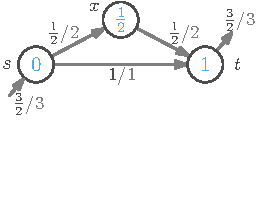
\includegraphics[scale=1,page=1]{networkAnalyzes/figures/tum_counter_example.pdf}
    % 
    \caption[\gls{tum} counter example.]{% 
        % 
        A~\gls{tum} counter example with three vertices with
        \textcolor{THETA}{voltage angles~\glssymbol{voltageangle}} that are
        written in the vertices, flows~\glssymbol{flow} and
        capacities~\glssymbol{capacity} are written on the edges~$
            % 
            \textcolor{KITblack70}{\glssymbol{flow}}
            /
            \textcolor{CAPACITY}{\glssymbol{capacity}}
            % 
        $. This example shows that flows are not necessarily integral, since the
        edges~$
            % 
            (\source, x), 
            (x,\sink)
            \in
            \glssymbol{edges}
            % 
        $ have each a flow of~$\textcolor{KITblack70}{\nicefrac{1}{2}}$.
        % \vspace{-15mm}
        % 
    }%
    %
    \label{ch:network-analyzes:fig:tum-counter-example}%
    % 
\end{wrapfigure}%
% 
Another application, where the rank of the matrix can be used is to check
whether a network with a given set of sensors is observable (\ie, all other
variables can be calculated by the measured ones). \textcite[p.487;(47)]{Kal59}
uses the property that if a set of vectors is linear independent then the system
becomes observable. Note that another way to prove the uniqueness was given
by~\textcite[p.114; Lemma 4.2.1]{Ver10} and~\textcite[p.361]{Roc84}.

\noindent A system of linear inequalities represents a convex polytope~$
    % 
    \polyhedron
    =
    \{
        \vv{\glssymbol{flow}} \in \reals^{\fmagnitude{ \glssymbol{edges} } }
        \mid
        \constraintmatrix
        \vv{ \glssymbol{flow} }
        \leq
        \frighthandsidevector{\constraintmatrix} 
    \}
    % 
$. Let~$\cuts_{i}$ be a hyperplane defined by~$
    % 
    \cuts_{i} 
    \coloneqq 
    \{
        \vv{\glssymbol{flow}}
        \in
        \reals^{ \fmagnitude{ \glssymbol{edges} } }
        \mid
        \constraintmatrix_i
        \cdot
        \vv{\glssymbol{flow}}
        =
        \frighthandsidevector{\constraintmatrix}_i 
    \}
    % 
$ that represents the~$i^{\mathrm{th}}$ row with~$
    % 
    1
    \leq 
    i
    \leq
    \fmagnitude{\glssymbol{edges}}
    % 
$. The cuts of a convex polytope~\polyhedron with each hyperplane~$\cuts_{i}$ is
given by~$
    % 
    \{
        \polyhedron
        \cap
        \cuts_{i}
        \mid
        1 \leq i \leq \fmagnitude{\glssymbol{edges}}
    \}
    % 
$ and represents the set of faces that form a \emph{convex hull}. 

Consider any objective then an optimal solution of a convex polytope~\polyhedron
is on the vertices of~\polyhedron. Thus, if the vertices of a convex
polytope~\polyhedron lie on integral coordinates than~\polyhedron is called
an~\emph{integral polytope}. If all square submatrices of~\constraintmatrix have
a determinant of~$-1, 0,$ or~$1$ then~\constraintmatrix is~\gls{tum}. This in
particular means that the polytope of such a~\gls{tum} matrix is integral
independent on the vector~$
    % 
    \frighthandsidevector{\constraintmatrix}
    % 
$.

Recall that we know that the incidence
matrix~\glssymbol{incidenceMatrix} and circuit matrix~\glssymbol{cycleMatrix}
are each~\gls{tum} by itself
(see~\cref{ch:network-analyzes:sec:mathematical-model:lem:I-and-B-TUM-sep}). In
the following, we prove that the whole system~$
    % 
    \constraintmatrix 
    \coloneqq 
    \binom{ 
        \glssymbol{incidenceMatrix} 
    }{ 
        \glssymbol{cycleMatrix} 
    }
    % 
$ is not~\gls{tum} and thus, the convex polytope is not necessarily integral.
% 
\begin{lemma}
% 
The bases of the incidence matrix~\glssymbol{incidenceMatrix} and the circuit
matrix~\glssymbol{cycleMatrix} are each~\gls{tum}. However, the whole system
of linear equations~$
% 
\constraintmatrix 
\coloneqq 
\binom{ 
    \glssymbol{incidenceMatrix} 
}{ 
    \glssymbol{cycleMatrix} 
}
% 
$ to compute a feasible electrical flow using the~\gls{kcl}
(\cref{ch:network-analyzes:sec:mathematical-model:eq:kcl-matrix-writing})
and~\gls{kvl}
(\cref{ch:network-analyzes:sec:mathematical-model:eq:kvl-matrix-writing}) is
not~\gls{tum}.
% 
\label{ch:network-analyzes:sec:mathematical-model:lem:pf-matrix-is-tum}
% 
\end{lemma}
% 
\begin{proof}
    % 
    A counter example is shown
    in~\cref{ch:network-analyzes:fig:tum-counter-example} that basically
    describes why a feasible electrical flow~\glssymbol{flow} is not integral
    for every right hand-side vector~$\frighthandsidevector{\constraintmatrix}$.
    % 
\end{proof}%

The~\gls{kcl}
(see~\cref{ch:network-analyzes:sec:mathematical-model:eq:kcl-matrix-writing})
and the~\gls{kvl}
(see~\cref{ch:network-analyzes:sec:mathematical-model:eq:kvl-matrix-writing}) do
not incorporate network elements in any sense---\ie, these equations are purely
topological~\parencite[p.127; Section 6-3]{Ses61}---the vector of voltage angle
differences~$\vv{\glssymbol{voltageangledifference}}$ can be replaced by the
flow vector~$\vv{\glssymbol{flow}}$. 

\begin{figure}
    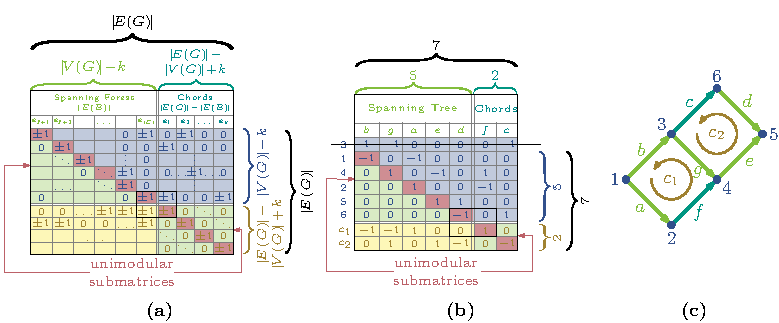
\includegraphics{networkAnalyzes/figures/Tum-proof.pdf}
     % 
    \caption[The combined incidence and circuit matrix structure.]{The structure
    of the matrix~$
    % 
        \constraintmatrix 
        \coloneqq 
        \binom{
            \textcolor{KITseablue}{\glssymbol{incidenceMatrix}}
        }{
            \textcolor{KITbrown}{\glssymbol{cycleMatrix}}
        }
    % 
    $ that is a construction of the \textcolor{KITseablue}{incidence
    matrix~\glssymbol{incidenceMatrix}} (top partition) and
    \textcolor{KITbrown}{circuit matrix~\glssymbol{cycleMatrix}} (bottom
    partition). The~\textcolor{KITpalegreen}{left partition} of
    size~$\textcolor{KITpalegreen}{\fmagnitude{\glssymbol{vertices}}-k}$,
    with~$k$ being the number of connected components (for (b) and (c) with one
    connected component~$k=1$), represents
    some~\textcolor{KITpalegreen}{spanning forest} (for $k=1$
    a~\textcolor{KITpalegreen}{spanning tree}) of the graph~\glssymbol{graph}.
    The~\textcolor{KITgreen}{right partition} represents the edges that are not
    in the~\textcolor{KITpalegreen}{spanning forest} of the left partition (also
    called~\textcolor{KITgreen}{chords}). The latter partition has a size
    of~$
        \textcolor{KITgreen}{%
            \fmagnitude{\glssymbol{edges}}%
            -
            \fmagnitude{\glssymbol{vertices}}%
            + k
        }%
        % 
    $. The green areas have entries that are all zero and the main diagonal with
    entries all~$\pm 1$ is marked in red. The general structure is given in (a)
    and a small example is given in (b) with the corresponding graph in (c).}%
    % 
    \label{ch:network-analyzes:sec:mathematical-model:fig:TUM-proof}%
\end{figure}
% 
Let~$\tree$ be a spanning tree in~$\glssymbol{graph}$. The
matrix~$
    % 
    \constraintmatrix
    \coloneqq
    \binom{
        % 
        \glssymbol{incidenceMatrix}_{%
            \glssymbol{edges}(\tree)%
        }\quad\glssymbol{incidenceMatrix}_{%
            \glssymbol{edges}(\glssymbol{graph})%
            \setminus%
            \glssymbol{edges}(\tree)%
        }% 
        % 
    }{
        % 
        \glssymbol{cycleMatrix}_{%
            \glssymbol{edges}(\tree)%
        }\quad\glssymbol{cycleMatrix}_{%
            \glssymbol{edges}(\glssymbol{graph})%
            \setminus%
            \glssymbol{edges}(\tree)%
        }%
        % 
    }
    % 
$ can be decomposed into two parts column-wise represented by the partitions
that are the set~$\glssymbol{edges}(\tree)$ of spanning tree edges
(see~\cref{ch:network-analyzes:sec:mathematical-model:fig:TUM-proof}\screen{a}
left top and bottom partition) and the set~$
    % 
    \glssymbol{edges}(\glssymbol{graph})
    \setminus
    \glssymbol{edges}(\tree)
    % 
$ of chords
(see~\cref{ch:network-analyzes:sec:mathematical-model:fig:TUM-proof}\screen{a}
right top and bottom partitions) for some arbitrary but fixed spanning
tree~\tree. The partition of the rows into two parts is given by construction~$
    % 
    \constraintmatrix
    =
    \binom{
        \glssymbol{incidenceMatrix}
    }{
        \glssymbol{cycleMatrix}
    }
    % 
$. Recall that all maximum square non-singular submatrices (\ie, matrices that
have a nonzero determinant) of the incidence
matrices~\glssymbol{incidenceMatrix} of size~$
    % 
    (\fmagnitude{\glssymbol{vertices}}-1)
    \times
    (\fmagnitude{\glssymbol{vertices}}-1)
    % 
$ are formed by some spanning tree~$\tree\in\mathcal T$ and submatrices of 
the
circuit matrix~\glssymbol{cycleMatrix} of size~$
    % 
    (\fmagnitude{\glssymbol{edges}} - \fmagnitude{\glssymbol{vertices}} + 1)
    \times
    (\fmagnitude{\glssymbol{edges}} - \fmagnitude{\glssymbol{vertices}} + 1)
    % 
$ that are formed by a set of chords, are unimodular (\ie, the
determinant is~$\pm 1$; 
see~\cref{ch:network-analyzes:sec:mathematical-model:fig:TUM-proof} top left
and bottom right partition, respectively). The structure allows us to permute
the entries such that the main diagonal has only~$\pm 1$ entries 
(see~\cref{ch:network-analyzes:sec:mathematical-model:fig:TUM-proof}\screen{a}
and~\screen{b} for example). We describe in the following how we permute the
matrix~\constraintmatrix.

We can order the rows and columns of the incidence
matrix~\glssymbol{incidenceMatrix} that are in the spanning tree partition
(see~\cref{ch:network-analyzes:sec:mathematical-model:fig:TUM-proof}\screen{a}
and~\screen{b} top left partition) such that entries below the diagonal are all
zero in that partition. This particular form of a matrix is denoted by the term
\emph{upper triangular matrix}. A property of the incidence
matrix~\glssymbol{incidenceMatrix} is that it has at most two non-zero entries
per column. In addition, the number of leaves~$
    % 
    \mathcal{L}
    \coloneqq
    {\{
        \vertexa
        \in
        \glssymbol{vertices}
        \mid
        \degree(\vertexa) 
        = 
        1
    \}}
    % 
$ in a spanning tree depend on the degree of the vertices meaning~$
    % 
    \fmagnitude{\mathcal{L}} 
    \geq
    \max_{\vertexa\in\glssymbol{vertices}}
    \degree (\vertexa)
    % 
$, which means that there is always enough space to the right of the diagonal.
To construct an upper triangular matrix in~\constraintmatrix
(see~\cref{ch:network-analyzes:sec:mathematical-model:fig:TUM-proof}\screen{a}),
we perform a~\acrlong{bfs} (\gls{bfs}). The~\gls{bfs} processes the inner
vertices of the spanning tree first and at the end all leaves. Using the
aforementioned observation of the number of leaves, we know that there is always
enough space to the right of the main diagonal. For the chord partition of the
circuit matrix~\glssymbol{cycleMatrix}, we are always able to adjust the entries
such that the lower and upper triangle of the matrix have zero entries only
(\cref{ch:network-analyzes:sec:mathematical-model:fig:TUM-proof}\screen{a}
and~\screen{b}; bottom right partition).
% 
We describe the~\gls{bfs} in the following.
 
Let~\tree be an arbitrary but fixed spanning tree and
let~\glssymbol{cycleMatrix} be the base of the columns of the circuit matrix
constructed from spanning tree~\tree. We start at some
vertex~$\vertexa\in\glssymbol{vertices}(\glssymbol{graph})$
(see~\cref{ch:network-analyzes:sec:mathematical-model:fig:TUM-proof}\screen{c}
vertex~$3$) and process its incident edges~$
    % 
    \{\vertexa,\vertexb\}
    \in
    \glssymbol{undirectededges}(\tree)
    % 
$. We add the columns of the incident edges to an empty
matrix~$\constraintmatrix'$ and the adjacent vertices~$
    % 
    \vertexb
    \in
    \glssymbol{vertices}(\glssymbol{graph})
    % 
$ as row. We proceed the aforementioned procedure with the next row's
vertex~\vertexb. Afterwards, we add the cycles~$\cycle\in\cycles$ that are in
the circuit matrix base~$\cycleMatrix$. Since each cycle in the base contributes
one nonzero chord entry, we add for each cycle the corresponding chord column~$
    % 
    \undirectededge
    \in
    \glssymbol{undirectededges}(\glssymbol{graph})
    \setminus
    \glssymbol{undirectededges}(\tree)
    % 
$. The resulting matrix is of the form~$
    % 
    \constraintmatrix'%
    \coloneqq%
    \binom{%
        % 
        \glssymbol{incidenceMatrix}_{%
            \glssymbol{edges}(\tree)%
        }\quad\glssymbol{incidenceMatrix}_{%
            \glssymbol{edges}(\glssymbol{graph})%
            \setminus%
            \glssymbol{edges}(\tree)%
        }% 
        % 
    }{%
        % 
        \glssymbol{cycleMatrix}_{%
            \glssymbol{edges}(\tree)%
        }\quad\glssymbol{cycleMatrix}_{%
            \glssymbol{edges}(\glssymbol{graph})%
            \setminus%
            \glssymbol{edges}(\tree)%
        }%
        % 
    }
    % 
$. We can conclude this discussion with the following lemma.
% 
\begin{lemma}
    % 
    Let~$
        % 
        \constraintmatrix 
        = 
        \binom{
            \glssymbol{incidenceMatrix}
        }{  
            \glssymbol{cycleMatrix}
        }
        % 
    $ be the matrix formed by the incidence matrix~\glssymbol{incidenceMatrix}
    and circuit matrix~\glssymbol{cycleMatrix}. The matrix's columns and rows
    can be permuted such that we get the form shown
    in~\cref{ch:network-analyzes:sec:mathematical-model:fig:TUM-proof}\screen{a}.
    % 
\end{lemma}
% 
To investigate the~\gls{tum} property, we take a look at the intersections of
the matrix~\constraintmatrix that are represented by all four partitions
(see~\cref{ch:network-analyzes:sec:mathematical-model:fig:TUM-proof}\screen{a}).
Thus, we distinguish between the following three main cases.
% 
\begin{compactenum}[\hspace*{3mm}\textbf{Case} 1\textbf{:}]
    % 
    \item The intersection between the chord and spanning tree partition of
    \label{ch:network-analyzes:sec:mathematical-model:cases:1}
    % 
    \begin{compactenum}[\hspace*{-11mm}(a)]
        % 
        \item the incidence matrix~\glssymbol{incidenceMatrix} (\cref{ch:network-analyzes:sec:mathematical-model:fig:TUM-proof}\screen{a}
        \&~\screen{b}; top left and top right partition),
        % 
        \label{ch:network-analyzes:sec:mathematical-model:cases:1a}
        % 
        \item the circuit matrix~\glssymbol{cycleMatrix} 
        (\cref{ch:network-analyzes:sec:mathematical-model:fig:TUM-proof}\screen{a}
        \&~\screen{b}; bottom left and bottom right partition).
        % 
        \label{ch:network-analyzes:sec:mathematical-model:cases:1b}
        % 
    \end{compactenum}
    % 
    \item The intersection between the incidence matrix~\glssymbol{incidenceMatrix}
    and the circuit matrix~\glssymbol{cycleMatrix} of
    \label{ch:network-analyzes:sec:mathematical-model:cases:2}
    % 
    \begin{compactenum}[\hspace*{-11mm}(a)]
        % 
        \item the spanning tree partition 
        (\cref{ch:network-analyzes:sec:mathematical-model:fig:TUM-proof}\screen{a}
        \&~\screen{b}; top left and bottom left partition), 
        % 
        \label{ch:network-analyzes:sec:mathematical-model:cases:2a}
        % 
        \item the chord partition 
        (\cref{ch:network-analyzes:sec:mathematical-model:fig:TUM-proof}\screen{a}
        \&~\screen{b}; top right and bottom right partition).
        % 
        \label{ch:network-analyzes:sec:mathematical-model:cases:2b}
        % 
    \end{compactenum}
    % 
    \item The intersection of all four partitions.
    \label{ch:network-analyzes:sec:mathematical-model:cases:3}
    % 
\end{compactenum}
% 
Since each matrix is~\gls{tum} by itself
Case~\ref{ch:network-analyzes:sec:mathematical-model:cases:1} is unproblematic
(see~\cref{ch:network-analyzes:sec:mathematical-model:lem:I-and-B-TUM-sep}). In
Case~\ref{ch:network-analyzes:sec:mathematical-model:cases:2}, we are already
able to find a square submatrix with determinant unequal~$\pm 1$ or~$0$
(see~\cref{ch:network-analyzes:sec:mathematical-model:fig:TUM-proof}\screen{b}
row~$5$ columns~$e$ and~$d$). 
% 
% In Case~\ref{ch:network-analyzes:sec:mathematical-model:cases:1a}, it is
% possible to get a submatrix where both diagonals are all~$\pm 1$. The latter
% case happens when there are multi-edges in the graph. These multi-edges have the
% property of being anti-symmetric and thus, the determinant is~$0$. For
% Case~\ref{ch:network-analyzes:sec:mathematical-model:cases:1b}, it is only
% possible that one diagonal is~$\pm 1$, since the chord matrix's triangles have
% only zero entries.
% 
% Now we come to Case~\ref{ch:network-analyzes:sec:mathematical-model:cases:2}. We
% start with the intersection of the two spanning tree partitions
% (Case~\ref{ch:network-analyzes:sec:mathematical-model:cases:2a}; left matrix
% partition
% in~\cref{ch:network-analyzes:sec:mathematical-model:fig:TUM-proof}\screen{a}).
% We mentioned above that we are always able to construct an incidence
% matrix~\glssymbol{incidenceMatrix} in such a way that the main diagonal of the
% matrix is~$\pm 1$ and that we get a triangle that has zero entries only either
% above or below the main diagonal
% (see~\cref{ch:network-analyzes:sec:mathematical-model:fig:TUM-proof}\screen{a}
% or~\screen{b}; green triangle in the top left partition). Thus, the only case
% where we get a diagonal is by using the last~$\pm 1$ entry of the main diagonal
% close to the intersection. However, since the other diagonal is always zero
% (since the triangle of~\glssymbol{incidenceMatrix} is all zero) these matrices
% are always unimodular. The same argument can be used for the chord section
% (Case~\ref{ch:network-analyzes:sec:mathematical-model:cases:2b}), since the
% chord partition of the circuit matrix has~$\pm 1$ on the main diagonal only.
% 
In Case~\ref{ch:network-analyzes:sec:mathematical-model:cases:3} it is also
possible to construct a graph such that there is a submatrix, where the
determinant is~$2$ (see the example
in~\cref{ch:network-analyzes:sec:mathematical-model:fig:TUM-proof}\screen{a}
and~\screen{b}). Inverting the direction of all cycles or edges has no influences
on the determinant. Same holds for
Case~\ref{ch:network-analyzes:sec:mathematical-model:cases:2}. Note that
inverting the direction of the edges does not help, since the direction changes
in the incidence and circuit matrix and thus, it only changes the sign of the
determinant.

Assume that a flow is a function~$
    % 
    \glssymbol{flow}
    \colon
    \glssymbol{edges}
    \to
    \integers
    % 
$ that is an integral flow, we get a system of integral equations (IE). Such
integral systems of equations or~\gls{ilp}s are usually a hint that the
underlying problem is~\NP-hard~\parencite[p.245; MP1]{Gar79}. A relaxation of
the function~\glssymbol{flow} (\ie, mapping to~\reals instead of~\integers) does
not necessarily yield an integral solution, since the polytope vertices do not
lie on integral coordinates 
(see~\cref{ch:network-analyzes:sec:mathematical-model:lem:pf-matrix-is-tum}).

Thus, with this technique we are not able to solve the problem
by~\textcite[pp.17ff.; Theorem~4.1]{Fel13} in polynomial time. However,
in~\cref{ch:network-analyzes:sec:scalability-power-flow} we see a technique that
leads to an integral electrical flow. Another possibility would be to restrict
the algorithm in~\cref{ch:network-analyzes:sec:algorithm} to integral flows
only.
% 
%%%%%%%%%%%%%%%%%%%%%%%%%%%%%%%%%%%%%%%%%%%%%%%%%%%%%%%%%%%%%%%%%%%%%%%%%%%%%%%%
\subsection{Scalability of Electrical Flows}
\label{ch:network-analyzes:sec:scalability-power-flow}
%%%%%%%%%%%%%%%%%%%%%%%%%%%%%%%%%%%%%%%%%%%%%%%%%%%%%%%%%%%%%%%%%%%%%%%%%%%%%%%%
% 
As already mentioned by~\textcite[p.114]{Gol89} a lot of flow algorithms use
scaling techniques. Whether it is the scaling of the capacity---introduced
by~\textcite{Edm72}---or the scaling of the excess that was introduced
by~\textcite{Ahu89}. For electrical flows, we will use scaling, too.
% 
The following scaling lemma follows directly
from~\cref{ch:network-analyzes:sec:mathematical-model:eq:KCL-intermediate-vertex,ch:network-analyzes:sec:mathematical-model:eq:KCL-generator-vertex,ch:network-analyzes:sec:mathematical-model:eq:KCL-consumer-vertex,ch:network-analyzes:sec:mathematical-model:eq:kvl-ohm-function-writing}.
% 
\begin{lemma}[Scaling]
    Every non-zero electrical
    flow~$\glssymbol{flow}'\colon\glssymbol{edges}\to\reals_{>0}$ can be
    rescaled to a feasible electrical flow~\glssymbol{flow} by applying a
    scaling factor~$\chi$, where
    % 
    {
    \small
    \begin{equation*}
            \MIN{\chi}%0
        \coloneqq
            \max
            \left(
                \max_{\vertexa\in\glssymbol{consumers}}
                \frac{
                    \glssymbol{realpowerdemandmin}(\vertexa)
                }{
                    \glssymbol{realpowerdemand}(\vertexa)
                },
                % 
                \max_{\vertexa\in\glssymbol{generators}}
                \frac{
                    \glssymbol{realpowergenerationmin}(\vertexa)
                }{
                    \glssymbol{realpowergeneration}(\vertexa)
                },
            \right)
        \leq
            \chi 
        \leq
            \min
            \left(
                \min_{\edge'\in\glssymbol{edges}}
                \frac{\glssymbol{capacity}(\edge')}{\glssymbol{flow}'(\edge')},
                % 
                \min_{\vertexa\in\glssymbol{consumers}}
                \frac{
                    \glssymbol{realpowerdemandmax}(\vertexa)
                }{
                    \glssymbol{realpowerdemand}(\vertexa)
                },
                % 
                \min_{\vertexa\in\glssymbol{generators}}
                \frac{
                    \glssymbol{realpowergenerationmax}(\vertexa)
                }{
                    \glssymbol{realpowergeneration}(\vertexa)
                }
            \right)
        \eqqcolon 
            \MAX{\chi}
    \end{equation*}
    }
    % 
    to~$\glssymbol{flow}(\edge) = \glssymbol{flow}'(\edge)\cdot~\chi$ for
    all~$\edge\in\glssymbol{edges}$.
    % 
    \label{ch:network-analyzes:sec:mathematical-model:lem:rescalling-an-pf}
\end{lemma}
% 
\begin{proof}
    Assume~$\vv{\glssymbol{flow}}'$ is an electrical flow
    complying~\cref{ch:network-analyzes:sec:mathematical-model:eq:kcl-matrix-writing,ch:network-analyzes:sec:mathematical-model:eq:kvl-matrix-writing}
    or
    alternatively~\cref{ch:network-analyzes:sec:mathematical-model:eq:KCL-intermediate-vertex,ch:network-analyzes:sec:mathematical-model:eq:KCL-generator-vertex,ch:network-analyzes:sec:mathematical-model:eq:KCL-consumer-vertex,ch:network-analyzes:sec:mathematical-model:eq:kvl-ohm-function-writing}.
    Multiplying~$\vv{\glssymbol{flow}}'$ by a scalar~$\chi$ yields in a
    flow~$\chi\cdot\vv{\glssymbol{flow}}' = \vv{\glssymbol{flow}}$ that is still
    an electrical flow, since it is only a scaling of an unrestricted vector.
    The latter means that
    multiplying~\cref{ch:network-analyzes:sec:mathematical-model:eq:kcl-matrix-writing,ch:network-analyzes:sec:mathematical-model:eq:kvl-matrix-writing}
    (assuming~$
    \glssymbol{voltageangledifference}\equiv\glssymbol{flow}$) by a scalar 
    (standard operation on a field) yields in a magnitude increase of all
    vectors including~$\vv{\glssymbol{flow}}$. However, to scale an electrical
    flow to a feasible electrical flow the flow has to comply with the capacity
    constraints 
    (\cref{ch:network-analyzes:sec:mathematical-model:eq:capacity-constraint}).
    
    For~$\chi \leq \MAX{\chi}$ we have
    % 
    \begin{align*}
        % 
        \glssymbol{flow}(\edge) 
        &= 
            \chi 
            \cdot 
            \glssymbol{flow}'(\edge)
        \\
        &\leq 
            \MAX{\chi} 
            \cdot 
            \glssymbol{flow}'(\edge)
        \\
        &= 
            \min_{\edge'\in\glssymbol{edges}} 
            \frac{
                \glssymbol{capacity}(\edge')
            }{
                \glssymbol{flow}'(\edge')  
            }
            \cdot
            \glssymbol{flow}'(\edge)
        \\
        &\leq
            \frac{
                \glssymbol{capacity}(\edge)
            }{
                \glssymbol{flow}'(\edge)  
            }
            \cdot
            \glssymbol{flow}'(\edge)
        \\
        &=
            \glssymbol{capacity}(\edge).
        % 
    \end{align*}
    % 
    Note that we included the maximum generation and demand~$
        % 
        \glssymbol{realpowergeneration} 
        = 
        \chi
        \cdot
        \glssymbol{realpowergeneration}'(\vertexa)
        \leq
        \MAX{\chi}
        \cdot
        \glssymbol{realpowergeneration}'(\vertexa)
        =
        \min_{\vertexa\in\glssymbol{generators}} 
        \nicefrac{
            \glssymbol{realpowergenerationmax}(\vertexa)
        }{
            \glssymbol{realpowergeneration}'(\vertexa)    
        }
        \cdot
        \glssymbol{realpowergeneration}'(\vertexa)    
        =
        \glssymbol{realpowergenerationmax}(\vertexa)
        % 
    $.
    % 
    % Thus, the scalar~$\chi$ is restricted by~$\chi\cdot\glssymbol{flow}'
    % (\edge)\leq\glssymbol{capacity}(\edge)$
    % meaning~$\chi\leq\nicefrac{\glssymbol{capacity}
    % (\edge)}{\glssymbol{flow}'(\edge)}$ for all~$\edge\in\glssymbol{edges}$.
    % This restricts the maximum scalar~$\MAX{\chi}$ for scaling by the smallest
    % value of~$\nicefrac{\glssymbol{capacity} (\edge)}{\glssymbol{flow}'(\edge)}$
    % for all~$\edge\in\glssymbol{edges}$. A scaling that is always feasible
    % is~$\chi = 0$
    % (see~\cref{ch:network-analyzes:sec:mathematical-model:eq:kcl-matrix-writing,ch:network-analyzes:sec:mathematical-model:eq:kvl-matrix-writing}), 
    % which represents a lower bound. Thus, $
    %     \vv{\glssymbol{flow}}
    %     =
    %     \vv{\glssymbol{flow}}'
    %     \cdot
    %     \chi
    % $ represents a feasible electrical flow
    % with~$0\leq\chi\leq\MAX{\chi}$.
\end{proof}
% 
Note that the last lemma would be much simpler if we make the bounded network to
an unbounded network. For this we will
use~\cref{lem:bounded_unbounded_mtsf_transformation} on
Page~$\pageref{lem:bounded_unbounded_mtsf_transformation}$ (see
also~\cref{ch:switching:sec:network_modeling:fig:bounded_unbounded_mtsf_transformation}).
% 
\begin{lemma}[Scaling Restatement]
    % 
    Let~$\dcnetworktuple$ be a power grid with minimum and maximum generations
    and demands. We model the upper and lower bounds of the generations and
    demands in the same fashion as
    in~\cref{lem:bounded_unbounded_mtsf_transformation}
    (\cref{ch:switching:sec:network_modeling:fig:bounded_unbounded_mtsf_transformation}~on
    page~\pageref{ch:switching:sec:network_modeling:fig:bounded_unbounded_mtsf_transformation}) 
    as lower and upper capacities. The edge capacities are~$
        % 
        \MIN{\glssymbol{capacity}}
        \equiv
        0
        % 
    $ and~$
        % 
        \MAX{\glssymbol{capacity}}
        \equiv
        \glssymbol{capacity}
        % 
    $. Every non-zero electrical flow~$
        % 
        \glssymbol{flow}'
        \colon
        \glssymbol{edges}
        \to
        \reals_{>0}
        % 
    $ can be rescaled to a feasible electrical flow~\glssymbol{flow} by applying
    a scaling factor~$\chi$, where
    % 
    {
    \small
    \begin{equation*}
            \MIN{\chi}%0
        \coloneqq
            \max_{\edge'\in\glssymbol{undirectededges}}
            \frac{
                \MIN{\glssymbol{capacity}}(\edge')
            }{
                \glssymbol{flow}'(\edge')
            }
        \leq
            \chi 
        \leq
            \min_{\edge'\in\glssymbol{undirectededges}}
            \frac{
                \MAX{\glssymbol{capacity}}(\edge')
            }{
                \glssymbol{flow}'(\edge')
            }
            % 
        \eqqcolon 
            \MAX{\chi}
    \end{equation*}
    }
    % 
    to~$\glssymbol{flow}(\edge) = \glssymbol{flow}'(\edge)\cdot~\chi$ for
    all~$\edge\in\glssymbol{edges}$.
    % 
    \label{ch:network-analyzes:sec:mathematical-model:lem:rescalling-an-pf}
\end{lemma}
% 
We can use the latter two results to up scale or down scale electrical flows.
% 
An~\source-\sink-network is a network with one
generator~$
    % 
    \{\source\}
    \eqqcolon
    \glssymbol{generators}
    % 
$ (\ie,
$\fmagnitude{\glssymbol{generators}} = 1$) and one consumer~$
    % 
    \{\sink\}
    \eqqcolon
    \glssymbol{consumers}
    % 
$ (\ie, $
    % 
    \fmagnitude{\glssymbol{consumers}}
    =
    1
    % 
$). Since there is a unique solution to a feasible electrical
flow~\glssymbol{flow}
(see~\cref{ch:network-analyzes:sec:mathematical-model:lem:unique-flow}) and we
can rescale every electrical flow by a factor~$\chi$
(\cref{ch:network-analyzes:sec:mathematical-model:lem:rescalling-an-pf}), we
chose an edge with the maximum violation of the capacity constraint, compute the
factor~$\MAX{\chi}$, and scale the flow on all edges in the network down
according to~$\MAX{\chi}$. The next lemma follows directly
from~\cref{ch:network-analyzes:sec:mathematical-model:lem:rescalling-an-pf},
since~$\MAX{\chi}$ is the largest possible scaling such that~$\vv{
\glssymbol{flow}}$ yields a feasible electrical flow. This flow represents the
maximum possible feasible electrical flow for an \source-\sink-network that is
equivalent to a~\gls{dc}~\acrlong{mpf} (\gls{dc}~\gls{mpf}). Note that
for~\source-\sink-networks there is only one controllable generator that means
the~\gls{mpf} is unique, too.
%
\begin{lemma}
    For an~\source-\sink-network~\glssymbol{network} any non-zero electrical
    flow~$\glssymbol{flow}'\colon\glssymbol{edges}\to\reals_{>0}$ can be
    rescaled to an~\acrshort{mpf} by using a scaling factor of~$\overline{\chi}$
    (see~\cref{ch:network-analyzes:sec:mathematical-model:lem:rescalling-an-pf}).
    % 
    \label{ch:network-analyzes:sec:mathematical-model:lem:rescalling-to-mpf}
    % 
\end{lemma}
% 
Note that for multiple generators the~\gls{mpf} is not necessarily unique,
since different real power generations~\glssymbol{realpowergeneration} can lead
to the same optimal value~$\opt_{\gls{mpfp}}(\glssymbol{network})$.

%%%%%%%%%%%%%%%%%%%%%%%%%%%%%%%%%%%%%%%%%%%%%%%%%%%%%%%%%%%%%%%%%%%%%%%%%%%%%%%% 
\subsection{Integral Electrical Flows}
\label{ch:network-analyzes:sec:mathematical-model:subsec:integral-power-flows}
%%%%%%%%%%%%%%%%%%%%%%%%%%%%%%%%%%%%%%%%%%%%%%%%%%%%%%%%%%%%%%%%%%%%%%%%%%%%%%%%
% 
In general, we can assume that the parameters of a~\gls{dc} power
grid~\glssymbol{network}, such as the susceptance~\glssymbol{susceptance}, are
rational~$\rationals$ and thus, the equations constitute a rational polytope,
since the cuts of the hyperplanes can only constitute rational numbers
(see~\cref{ch:network-analyzes:sec:mathematical-model:def:rational-polytope}).
% 
\begin{definition}[Rational Polytope; {{\textcite[p.61]{Sch03}}}]
    A system of linear inequalities of the
    form~$
    \{
        \vv{\glssymbol{flow}}
        \in
        \reals^m
        \mid
        \constraintmatrix
        \vv{\glssymbol{flow}}
        \leq
        \frighthandsidevector{\constraintmatrix}\}
    $,
    where~$
    \constraintmatrix
    \in
    \rationals^{n\times m}
    % 
    $ and~$
    % 
    \frighthandsidevector{\constraintmatrix}
    \in
    \rationals^{n}
    % 
    $, is called a~\emph{rational system of linear inequalities}. A rational
    system of linear inequalities constitutes a rational polytope. The latter
    means that all vertices of the polytope lie on rational coordinates. Such a
    rational polytope represents the convex hull of a finite set of rational
    vectors.
    % 
    \label{ch:network-analyzes:sec:mathematical-model:def:rational-polytope}
\end{definition}% 
% 
Naturally, feasible electrical flows are not integral
(see~\cref{ch:network-analyzes:sec:mathematical-model:lem:pf-matrix-is-tum}),
which means that feasible electrical flows are not integral for every right-hand
side vector~$\frighthandsidevector{ \constraintmatrix }$.
% 
Let~\glssymbol{flow} be a feasible electrical flow. If we neglect the capacity
constraints
(see~\cref{ch:network-analyzes:sec:mathematical-model:eq:capacity-constraint};
or equivalently define~$
    % 
    \glssymbol{capacity}
    \equiv
    \infty
    % 
$) and relax the generation and demand constraints.
% 
% , we are able to scale~\glssymbol{flow} to an
% integral electrical flow using the technique
% of~\cref{ch:network-analyzes:sec:mathematical-model:lem:rescalling-an-pf}.
% 
Assuming that the flow~$\glssymbol{flow}\in\rationals$ then we can rescale the
flow to an integral flow using the least common multiplier (LCM) and the
technique presented
in~\cref{ch:network-analyzes:sec:mathematical-model:lem:rescalling-an-pf}.
% 
% However, one may notice that
% by using the scaling argument, we neglect the capacity constraints, and relax
% the demand, and generation constraints. This relaxation leads us to integral
% electrical flow. We can get such a flow by using an arbitrary (feasible)
% electrical flow and scale it such that all flows are integral electrical flows
% using~\cref{ch:network-analyzes:sec:mathematical-model:lem:rescalling-an-pf}.
% Note that we ignore the capacity constraints
% (\cref{ch:network-analyzes:sec:mathematical-model:eq:capacity-constraint}).
% 
% Thus, if we assume that we model the generations and demands by an additional
% edge with corresponding capacities at the generators and demands, respectively,
% then we are always able to get a feasible integral electrical flow
% with~$\mincapacity(\source_{\vertexa},\vertexa)=\glssymbol{realpowergeneration}
% (\vertexa)$ for all~$\vertexa\in\glssymbol{generators}$
% and~$\mincapacity(\vertexa,\sink_{\vertexa})=\glssymbol{realpowerdemand}(\vertexa)$
% for all~$\vertexa\in\glssymbol{consumers}$ and upper bounds for the capacities
% of~$\MAX{\glssymbol{capacity}}\equiv\infty$.
% 
\begin{theorem}[Integral Electrical Flow]
    If there is a (nonzero) solution to an electrical flow~$\glssymbol{flow}$
    with~$\glssymbol{flow}\in\rationals$ then there is a nonzero integral
    electrical flow that can be reached by scaling.
    % 
    \label{ch:network-analyzes:sec:mathematical-model:thm}
\end{theorem}
%
Unfortunately, the scaling to integral electrical flows
(\cref{ch:network-analyzes:sec:mathematical-model:thm}) does not answer the
question of the worst case size of integral electrical flows. This highly
depends on the right-hand side vector.
% 
% 
%
% In our algorithm (see~\cref{ch:network-analyzes:sec:algorithm}) and the above
% question of if there exist any electrical flow on~\glssymbol{network} that is
% integral and has polynomial size, we can neglect capacities and thus, real power
% generation and demands, since we can always rescale the network according these
% capacities if necessary. 
% Note, if the zero flow is the only electrical flow then there is no electrical
% flow for~\glssymbol{network}.
% 
% \noindent In this section, we are basically interested in the following two
% questions.
% 
% \begin{compactenum}[(Q1)]
%     \item Is there a right hand side vector~$
%         \frighthandsidevector{\constraintmatrix}$ such that there is an
%         integral electrical flow vector~$\vv{\glssymbol{flow}}$ for a given
%         matrix~\constraintmatrix?
%     \item What is the size of a minimum integral solution~\glssymbol{flow}?
% \end{compactenum}
% % 
% We answered the first question by a scaling argument. However, the first
% question represents a generalization of~\gls{tum}, which represents a subproblem
% for every~\gls{ilp}. To answer the second question, we introduce~\acrlong{tdi}
% (\gls{tdi}), which represents a generalization of~\gls{tum}.
% % 
% \begin{definition}[Total Dual Integrality~(\gls{tdi}); {{\textcite[p.195;Section~7;Theorem 7.1']{Edm77}}}]
%     % 
%     A rational
%     system~$\constraintmatrix\vv{\flow}\leq\frighthandsidevector{\constraintmatrix}$
%     is \emph{total dual integral~(\gls{tdi})} if
%     $$\min(
%         \transpose{\vv{y}}
%         \frighthandsidevector{\constraintmatrix} 
%         \mid
%         \transpose{\vv{y}}
%         \constraintmatrix 
%         = 
%         \transpose{\vv{c}}, 
%         \vv{y} 
%         \geq 
%         \vv{0}
%     ) = \max(
%         \transpose{\vv{c}} 
%         \vv{\flow}
%         \mid
%         \constraintmatrix
%         \vv{\flow}
%         \leq
%         \frighthandsidevector{\constraintmatrix}
%     )$$
%     has an integral optimum dual solution~$\overline{y}$ for all
%     integral~$\transpose{c}\in\integers^n$ for which the dual program is finite.
%     % 
%     \label{ch:network-analyzes:sec:mathematical-model:def:TDI}
% \end{definition}
% %
% This basically means that~\gls{tdi} is a property of the whole system~$
% \constraintmatrix
% \vv{\flow}
% \leq
% \frighthandsidevector{\constraintmatrix}
% $ and not as for~\gls{tum} of the matrix~$\constraintmatrix$ itself. In the
% second question, we search for the \textquote{smallest} vector~$
% \frighthandsidevector{\constraintmatrix}$ such
% that the whole system is~\gls{tdi}. Scaling represents an affine transformation
% and~\gls{tdi} is a cutting with affine hyperplanes. 

% Recall from~\cref{ch:network-analyzes:sec:mathematical-model} and the proof
% of~\cref{ch:network-analyzes:sec:mathematical-model:lem:unique-flow} that our
% linear system of equation~\constraintmatrix has full rank. Thus, the
% polytope~\polyhedron is full-dimensional with~$\dimensionx{\polyhedron} =
% \fmagnitude{\glssymbol{edges}}$.
% Using~\cref{ch:network-analyzes:sec:mathematical-model:def:TDI-properties}, we
% see that our system of equations is~\gls{tdi}
% (see~\cref{ch:network-analyzes:sec:mathematical-model:def:TDI-properties}).
% % 
% \begin{lemma}[{{\textcite[p.12--4; Theorem~12.12]{online:Paf13}}}]
%     Let~\polyhedron be a rational polytope.
%     \begin{compactenum}
%         \item Then there is a~\gls{tdi} system~$\constraintmatrix
%         \vv{\glssymbol{flow}}\leq
%         \frighthandsidevector{\constraintmatrix}$ for an
%         integral matrix~$\constraintmatrix$ that defines~\polyhedron.
%         % 
%         \item Vector~$\frighthandsidevector{\constraintmatrix}$ can be chosen to
%         be integral if and only if~\polyhedron is integral.
%         % 
%         \item If~\polyhedron is full-dimensional, then there is a unique
%         minimal~\gls{tdi} system defining~\polyhedron.
%     \end{compactenum}
%     % 
%     \label{ch:network-analyzes:sec:mathematical-model:def:TDI-properties}
% \end{lemma}
% 
% \begin{corollary}[{{\textcite[p.12--4; Corollary~12.13]{online:Paf13}}}]
%     A rational polyhedron~\polyhedron is integral if and only if there is a
%     \gls{tdi}-system~$\constraintmatrix\vv{\flow}\leq\righthandsidevector$ with
%     integral~$\righthandsidevector$ that defines it.
%     % 
%     \label{ch:network-analyzes:sec:mathematical-model:lem:rational-P-integral}
% \end{corollary}
% 
% So far we just characterized our system to be~\gls{tdi}. The following lemma
% restricts the size of our integral solution.
% % 
% \begin{lemma}[{{\textcite[p.12--5; Corollary~12.15]{online:Paf13}}}]
%     If a rational system~$\constraintmatrix\vv{\flow} =
%     \frighthandsidevector{\constraintmatrix}$ of linear equations has an
%     integral solution, then it has one of size polynomially bounded in the size
%     of~\constraintmatrix and~\frighthandsidevector{\constraintmatrix}.
%     % 
%     \label{ch:network-analyzes:sec:mathematical-model:lem:rational-P-poly-size}
% \end{lemma}
% % 
% With that we answered the second question and conclude this section with the
% following result.
% % 
% \begin{theorem}[Polynomial Bounded Integral Flow]
%     The integral electrical flow is polynomially bounded in~\constraintmatrix
%     and~\frighthandsidevector{\constraintmatrix}.
%     % 
%     \label{ch:network-analyzes:sec:mathematical-model:lem:integral-e-flow-poly-size}
% \end{theorem}
%
%%%%%%%%%%%%%%%%%%%%%%%%%%%%%%%%%%%%%%%%%%%%%%%%%%%%%%%%%%%%%%%%%%%%%%%%%%%%%%%% 
\subsection{Planar Graphs}
\label{ch:network-analyzes:sec:mathematical-model:subsec:planar-graphs}
%%%%%%%%%%%%%%%%%%%%%%%%%%%%%%%%%%%%%%%%%%%%%%%%%%%%%%%%%%%%%%%%%%%%%%%%%%%%%%%%
%
We will focus on planar graph in this chapter, which we will introduce in this
section.
%
\begin{figure}
    % 
    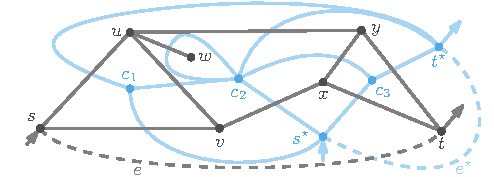
\includegraphics{networkAnalyzes/figures/Dual-Graph.pdf}
    % 
    \caption[Combinatorial dual graphs.]{A plane single-source~\source and
    single-sink~\sink graph~\textcolor{PRIMALGRAPH}{\glssymbol{graph}}
    (\textcolor{PRIMALGRAPH}{dark gray vertices~\tikzStandardVertex} and edges)
    and its combinatorial dual
    graph~\textcolor{DUALGRAPH}{\glssymbol{dualgraph}}
    (\textcolor{DUALGRAPH}{cyan blue vertices~\tikzStandardVertexDual} and
    edges). Adding the~\textcolor{PRIMALGRAPH}{edge~\edge}
    (\textcolor{PRIMALGRAPH}{dark gray dashed line}) divides the outer face into
    two faces representing the faces that include the dual
    source~$\textcolor{DUALGRAPH}{\source^\star}$ and dual
    sink~$\textcolor{DUALGRAPH}{\sink^\star}$ of the~\textcolor{DUALGRAPH}{dual
    graph}. Note that since we have a one-to-one correspondence of the edges,
    adding the edge~\textcolor{PRIMALGRAPH}{\edge} in~\textcolor{PRIMALGRAPH}
    {\glssymbol{graph}} is symmetrical to adding the
    edge~$\textcolor{DUALGRAPH}{\edge^\star}$
    in~\textcolor{DUALGRAPH}{\glssymbol{dualgraph}}.}
    % 
    \label{ch:network-analyzes:sec:mathematical-model:fig:graph-and-the-dual}
    % 
\end{figure}
% 
\textcite[p.13]{Cai12} mention that power grids are planar. A graph is
called~\emph{planar} if it can be embedded into the plane without any edge
crossings, \ie, the edges have no common point, but the two vertices
representing the endpoints of an edge. However, note that there is usually more
than one embedding for a graph~\glssymbol{graph} that is planar. Thus, let us
assume a fixed~\emph{planar embedding}~\glssymbol{embedding} of a
graph~\glssymbol{graph} into the plane
with~$\glssymbol{graph}(\glssymbol{embedding})\cong\glssymbol{graph}$ (\ie,
$\glssymbol{graph}(\glssymbol{embedding})$ is isomorphic to~\glssymbol{graph})
and an injective
function~$\embeddingMap\colon\glssymbol{vertices}\to\reals\times\reals$ meaning
there is a correspondence between the vertices~\glssymbol{vertices} of the graph
and the geometrical points~$\points$ of the plane embedding. An edge
set~$\glssymbol{edges}(\glssymbol{graph})$ of~$\glssymbol{graph}(\embedding)$ is
a subset of a topological space~$\mathcal{T}$, where each edge
in~$\glssymbol{graph}(\embedding)$ is a Jordan curve in~$\mathcal{T}$ and the
incidences and adjacencies are defined accordingly~\parencite{Gro01}.

For power grids such an embedding is usually given by the geographical location
of the network components, where~$\points$ represents the locations of the buses
in terms of latitude and longitude. In addition, we assume a
network~\dcnetworktuple with~$\fmagnitude{\glssymbol{generators}} = 1$
and~$\fmagnitude{\glssymbol{consumers}} = 1$. The vertices that represent the
single generator and single demand are denoted by source~\source and sink~\sink,
respectively.

For plane graphs, we have the concept of duality, which we will link with the
results of duality given
in~\cref{ch:network-analyzes:sec:mathematical-model:subsec:matroids-independence-systems}.
The geometric dual of a plane~\emph{primal graph}~\glssymbol{graph} is called
the~\emph{dual graph}~\glssymbol{dualgraph}. An example is given
in~\cref{ch:network-analyzes:sec:mathematical-model:fig:graph-and-the-dual}. To
construct a dual graph, we introduce the concept of a \emph{face}. We denote
faces by~\face. An \emph{inner face} is a region that is bounded by edges and
vertices in graph~\glssymbol{graph}. We say that these edges are incident to the
face.
% 
The \emph{outer face} is the unbounded region
(see~\cref{ch:network-analyzes:sec:mathematical-model:fig:graph-and-the-dual}
face~$\cycle_\sink$). The dual graph~\glssymbol{dualgraph} is constructed by
introducing a vertex for each face and connecting two vertices if the faces have
an edge in common. Note that we introduce an edge in the dual
graph~\glssymbol{dualgraph} for each edge in the primal graph~\gls{graph}.
% 
% Note that edges where both sides are incident to the same face introduce
% self-loops to the graph
% (see~\cref{ch:network-analyzes:sec:mathematical-model:fig:graph-and-the-dual}
% face~$\cycle_2$ and edge~$\{\vertexa,\vertexc\}$). 
% 
% Note that a self-loop shows that a face represents more than a cycle. However,
% in most cases we can simply
% apply~\cref{ch:network-analyzes:sec:mathematical-model:sim:loop_contraction} to
% reduce the graph. 
Note that a face might represent more than just a cycle, \eg, if
vertex~$\vertexc$
in~\cref{ch:network-analyzes:sec:mathematical-model:fig:graph-and-the-dual} is a
graph itself.
%
%%%%%%%%%%%%%%%%%%%%%%%%%%%%%%%%%%%%%%%%%%%%%%%%%%%%%%%%%%%%%%%%%%%%%%%%%%%%%%%% 
\subsection{Matroids and Independence Systems}
\label{ch:network-analyzes:sec:mathematical-model:subsec:matroids-independence-systems}
%%%%%%%%%%%%%%%%%%%%%%%%%%%%%%%%%%%%%%%%%%%%%%%%%%%%%%%%%%%%%%%%%%%%%%%%%%%%%%%%
% 
% The first two Kirchhoff's laws
% in~\cref{ch:network-analyzes:sec:mathematical-model:eq:kcl-matrix-writing,ch:network-analyzes:sec:mathematical-model:eq:kvl-matrix-writing},
% respectively, focus on the network topology only and do not consider any
% individual behavior of the electrical components (modeled on an edge) such as
% resistors.
% % 
% To cover the electrical components, the third Kirchhoff's law~
% \parencite{Kir47}\parencite[p. 127]{Ses61}
% incorporates these components in a more general sense. However, the third law is
% not relevant to this work and therefore not described formally here. The three
% laws describe the independence of the topology (\ie, \gls{kcl} and~\gls{kvl})
% and the network components (see~\textcite{Kir47}).
% 
% 
A lot of model transformations, properties, and relationships that we use in the
following with regard to matroids (see the postulates of~\textcite[p.510;
Theorem 1]{Whi35}) are based on the discussion by~\textcite{Ses61}
and~\textcite{Whi35,Whi31}. A matroid~\parencite{Whi35} represents a
generalization of a graph~\parencite{Whi31}.
% 
A \emph{matroid} is an abstraction of the independence term that is used in
different fields such as graph theory and geometry. Though different matroids
are considered in different fields, the consensus stays the same. We recall the
definition of a \emph{matroid} by~\textcite[pp.279]{Kor00} (first version was
given by~\textcite[p.510]{Whi35}). A \emph{matroid} is an ordered
pair~$(U,\mathcal{I})$, where~$U$ is the universe
and~$\mathcal{I}\subseteq\mathcal{P}(U)$ is an \emph{independence system}, which
satisfies the following three axioms.
% 
\begin{enumerate}[\textbf{Axiom}~1.]%
    \item $\emptyset\in\mathcal{I}$ (neutral element).
    \label{ch:network-analyzes:sec:mathematical-model:matroid:1}
    % 
    \item If $I\in\mathcal{I}$ and~$I'\subseteq I$ then~$I'\in\mathcal{I}$ 
    (monotonicity).%reflexivity 
    \label{ch:network-analyzes:sec:mathematical-model:matroid:2}
    % 
    \item If~$I_1, I_2\in\mathcal{I}$ with~$\fmagnitude{I_1} < \fmagnitude{I_2}$
    % and~$I_1\cap I_2\not=\emptyset$ 
    then there is an~$e\in (I_2\setminus I_1)$ such
    that~$I_1\cup\{e\}\in\mathcal{I}$ (augmentation).%transitivity
    % 
    \label{ch:network-analyzes:sec:mathematical-model:matroid:3}
\end{enumerate}
% 
Note that the Axiom~\ref{ch:network-analyzes:sec:mathematical-model:matroid:1}
and Axiom~\ref{ch:network-analyzes:sec:mathematical-model:matroid:2} represent
axioms that also hold for any independence system. However, the
Axiom~\ref{ch:network-analyzes:sec:mathematical-model:matroid:3} makes it a
matroid that is a generalization of the term linear independence.
% 
\textcite{Whi35} defines a~\emph{base} as a maximal independent submatroid and
a \emph{cycle} as a minimal dependent submatroid. 
%
\begin{definition}[{{\textcite[p.509]{Whi35}}}]
    A subgraph of a graph is independent if it contains no cycles. 
\end{definition}
% 
In this work, we use an important mathematical principle called \emph{duality}.
In different research areas it has different meanings. However, for us it
basically means that if there is a bijection between the edges (\ie, columns)
in~\glssymbol{incidenceMatrix} and the edges in~\glssymbol{cycleMatrix} and for
a submatroid~$\glssymbol{incidenceMatrix}'$ of~\glssymbol{incidenceMatrix} and
the corresponding dual~$\glssymbol{cycleMatrix}'$ in~$\glssymbol{cycleMatrix}$,
we have the relationship~$\rankx{\glssymbol{cycleMatrix}'} = \rankx{
\glssymbol{cycleMatrix}} - \nullityx{\glssymbol{incidenceMatrix}'}$, 
then~\glssymbol{incidenceMatrix} is a dual of~\glssymbol{cycleMatrix}
and~\glssymbol{cycleMatrix} is a dual
of~\glssymbol{incidenceMatrix}~\parencite[pp.521ff.]{Whi35}. The latter is called
\emph{involution} implying that the dual of the dual
of~\glssymbol{incidenceMatrix} is~\glssymbol{incidenceMatrix} itself. Though
\textquote{every matroid has a dual}~\parencite[p.522; Theorem~22]{Whi35} the
concept applies from a graph-theoretical perspective to plane graphs only. Only
plane graphs have a dual graph.

The following theorems state very central results that are used in this work.
% 
\begin{theorem}[{{\textcite[p.527; Theorem 31]{Whi35}}}]
    %
    For any graph~\glssymbol{graph} the matroids corresponding to its incidence
    matrix~\glssymbol{incidenceMatrix} and its circuit
    matrix~\glssymbol{cycleMatrix} are duals.
    %
    \label{ch:network-analyzes:sec:mathematical-model:thm:matrix-and-its-circuit-matrix-are-duals}
    % 
\end{theorem}
% 
For graphs we restricted the duality to plane graphs, since there is only a dual
graph if the primal graph is planar. For matroids this restriction does not hold
and thus, if we do not restrict ourself to the plane (\ie, sphere with
genus~$0$) but other surfaces with genus greater~$0$, we can still embed a
non-planar graph on a more complex surface without any crossing by making use of
the holes. An example is the embedding of the~$K_5$ on a torus (\ie, surface of
genus~$1$). Note that we focus on planar graph and genus~$0$.
% However, we focus on planar graph and genus 0. The primal matroid is
% the base of the incidence matrix and the dual matroid is the base of the circuit
% matrix.
 
The aforementioned duality
(see~\cref{ch:network-analyzes:sec:mathematical-model:thm:matrix-and-its-circuit-matrix-are-duals})
applies to the matroids~\glssymbol{incidenceMatrix} and~\glssymbol{cycleMatrix}.
% Recall that matroids are generalizations of graphs and thus, all results on
% matroids can be applied on graphs, too.
% 
%
The next theorem follows from
Axiom~\ref{ch:network-analyzes:sec:mathematical-model:matroid:2} and the
aforementioned discussion of the incidence matrix.
%
\begin{theorem}[{{\textcite[p.510; Theorem 1]{Whi35}}}]
    A set~$\glssymbol{incidenceMatrix}'\subseteq\glssymbol{incidenceMatrix}$
    is independent if and only if it is contained in a base, or, if and only if
    it contains no cycles.
\label{ch:network-analyzes:sec:mathematical-model:thm:basis-contain-no-cylces}
\end{theorem}
% 
% Recall that we talk about plane graphs and that only plane graphs have duals
% (see~\cref{ch:network-analyzes:sec:mathematical-model:subsec:planar-graphs}).
The next lemma follows
from~\cref{ch:network-analyzes:sec:mathematical-model:thm:matrix-and-its-circuit-matrix-are-duals}
and is illustrated
in~\cref{ch:network-analyzes:sec:mathematical-model:fig:graph-and-the-dual}.
%
\begin{lemma}[{{\textcite[p.85; Corollary 4-24]{Ses61}}}]
    % 
    If~$\glssymbol{graph}_1$ and~$\glssymbol{graph}_2$ are dual graphs, the
    incidence matrix of either
    graph is a circuit matrix of the other (with the proper rank, and each row
    representing a cycle); that is
    $$ \glssymbol{incidenceMatrix}_1 = \glssymbol{cycleMatrix}_2\text{ and }
    \glssymbol{incidenceMatrix}_2 = \glssymbol{cycleMatrix}_1.$$
    % 
    \label{ch:network-analyzes:sec:mathematical-model:cor:incidence-circuit-matrix-duals}
    % 
\end{lemma}
%
The lemma concludes the duality and is extensively used in this chapter
(see~\cref{ch:network-analyzes:sec:algorithm,ch:network-analyzes:simultaneous-flow-representation}).
% 
%
% 
\begin{figure}[t!]
    % 
    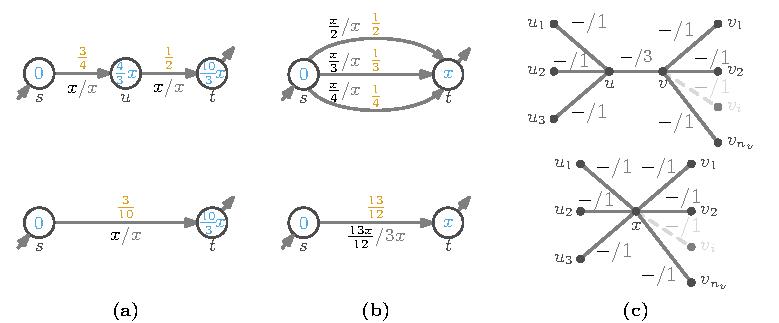
\includegraphics{networkAnalyzes/figures/Series-Parallel-Transformation.pdf}
    % 
    \caption[The series-parallel-contraction and contraction of superfluous
    edges.]{ Three example graphs in which we label each
    vertex~$\vertexa\in\glssymbol{vertices}$ that is represented by a
    cycle~\tikzVertex with a~\textcolor{THETA}{voltage
    angle~$\glssymbol{voltageangle}(\vertexa)$}. If the voltage angles are not
    important, we just use standard bullets~\tikzStandardVertex. On the edges,
    we write the flow~\glssymbol{flow} and the edge's
    capacity~\glssymbol{capacity} in the form~$\glssymbol{flow} /
    \textcolor{CAPACITY}{\glssymbol{capacity}}$. If
    the~\textcolor{SUSCEPTANCE}{susceptance~\glssymbol{susceptance}} is
    important for the transformation, we write it on the edge.

    The series-parallel-contraction and contraction of superfluous edges
    in energy networks simplifies the graph structure. (a) In a
    series-contraction a path is contracted to a single edge. (b) In a
    parallel-contraction multiple parallel edges (multi-edges) are contracted to
    one edge.
    % 
    (c)~A scenario where shortening of superfluous edges
    (\cref{ch:network-analyzes:sec:mathematical-model:sim:edge_shortening}) is
    reasonable. This figure is adapted from~\parencite[p.313; Figure~4]{Ake60}.
    The upper figure is an example, where the capacity of edge~$
    \glssymbol{capacity}(\vertexa,\vertexb)\geq\min\big(\sum_{
    \{\vertexa_i,\vertexa\}\in\glssymbol{edges}}\glssymbol{capacity}(\vertexa_i,\vertexa),\sum_{
    \{\vertexb_i,\vertexb\}\in\glssymbol{edges}}\glssymbol{capacity}(\vertexb_i,\vertexb)\big)$.
    In the bottom figure the resulting graph after contracting the superfluous
    edge~$\{\vertexa,\vertexb\}$
    to a vertex~$x$ is shown. 
    }
    % 
    \label{ch:network-analyzes:sec:mathematical-model:fig:SeriesParallelContraction}
\end{figure}
%
% 
%%%%%%%%%%%%%%%%%%%%%%%%%%%%%%%%%%%%%%%%%%%%%%%%%%%%%%%%%%%%%%%%%%%%%%%%%%%%%%%
\section{Electrical Preserving Transformations}
\label{ch:network-analyzes:sec:reduction-transformation-rules}
%%%%%%%%%%%%%%%%%%%%%%%%%%%%%%%%%%%%%%%%%%%%%%%%%%%%%%%%%%%%%%%%%%%%%%%%%%%%%%%
%
In this section, we introduce some standard reduction rules used in literature
that lead in the end to an algorithm to solve the~\gls{dc}~\gls{feas}. Most
transformations make use of the superposition principle for linear power grids,
\eg, the~\deltawye- and~\wyedelta-transformations. The superposition principle
holds (\ie, used for the superposition of, \eg, forces), since the constraint
matrix~\constraintmatrix is a linear map and thus, superposition becomes a
simple addition of linear equations (\ie, standard operation in a
field~$\mathbb{F}$). Though we give rules to compute the
capacity~\glssymbol{capacity}, these formulas can be dependent on the actual
flow
(see~\cref{ch:network-analyzes:sec:mathematical-model:sim:deltawye_transformation}).
Computing any electrical flow becomes trivial if we contract the graph to one
edge since on trees the electrical flow is equivalent to a graph-theoretical
flow~\parencite{Lei15b}\parencite[p.9; Lemma~4]{Leh15a}.

Recall that we have a unique electrical flow in~\source-\sink-graphs
(see~\cref{ch:network-analyzes:sec:mathematical-model:lem:unique-flow}), we can
scale it to a multiple such that it complies with the capacity constrains
(\cref{ch:network-analyzes:sec:mathematical-model:eq:capacity-constraint}).
Thus, we are able to neglect the capacity constraints and rescale the electrical
flow afterwards such that the capacity constraints are fulfilled
using~\cref{ch:network-analyzes:sec:mathematical-model:lem:rescalling-to-mpf}.
From
the~\cref{ch:network-analyzes:sec:mathematical-model:eq:KCL-intermediate-vertex,ch:network-analyzes:sec:mathematical-model:eq:KCL-generator-vertex,ch:network-analyzes:sec:mathematical-model:eq:KCL-consumer-vertex,ch:network-analyzes:sec:mathematical-model:eq:kvl-ohm-function-writing},
we have only one component that has a crucial influence on the electrical flow
and that is the susceptance~\glssymbol{susceptance}. The susceptance represents
a ratio that can be interpreted as how many electrons go through a path. Thus,
the notion of electrical preserving is purely susceptance based.
% 
\begin{definition}[Electrical Preserving Transformation]
    % 
    Let~\glssymbol{flow} be a given flow and let~$\glssymbol{voltageangle}
    (\vertexa)$ be the voltage angles before the transformation for
    all~$\vertexa\in\glssymbol{vertices}(\glssymbol{graph})$ with regard
    to~\glssymbol{flow}. An electrical preserving transformation~$\mathcal{T}$
    on~\glssymbol{network} is a function~$
    % 
        \mathcal{T}
        \colon 
            % \glssymbol{vertices} 
            % \times
            % \glssymbol{undirectededges}
            \mathcal M (\glssymbol{network})
            % \times
            % \glssymbol{susceptance} 
        \to %\glssymbol{vertices}
            %\times
            %\glssymbol{undirectededges}
            \mathcal M (\glssymbol{network})
            % \times
            % \glssymbol{susceptance}
    % 
    $ with~$
    % 
        (
        \glssymbol{graph} 
        =
        (
        \glssymbol{vertices},
        \glssymbol{undirectededges}
        ),
        \glssymbol{susceptance}
        ) 
        \mapsto 
        (
        \glssymbol{graph}'
        =
        (
            \glssymbol{vertices}',
            \glssymbol{undirectededges}'
        ),
        \glssymbol{susceptance}'
        )
    % 
    $ and new voltage angle assignments~$
        % 
        \glssymbol{voltageangle}'(\vertexa)
        % 
    $ for all~$\vertexa\in\glssymbol{vertices}'$ such that the susceptances are
     transformed in such a way that for the flow~\glssymbol{flow} we have~$
        %
        \glssymbol{voltageangle}'(\vertexa) 
        =
        \glssymbol{voltageangle}(\vertexa)
        % 
    $ for all vertices~$
        % 
        \vertexa
        \in
        (
            \glssymbol{vertices}
            \cap
            \glssymbol{vertices}'
        )
        % 
    $.
    % An electrical preserving transformation results in a susceptance that
    % preserves the initial susceptance ratio for each vertex pair that takes
    % part on the transformation.
    % 
    \label{ch:network-analyzes:sec:mathematical-model:def:electrical-preserving}
\end{definition}
% 
% However, if we have a network with a single generator and a single consumer it
% follows
% from~\cref{ch:network-analyzes:sec:mathematical-model:lem:rescalling-to-mpf}
% that we can neglect the capacities
% (see~\cref{ch:network-analyzes:sec:mathematical-model:eq:capacity-constraint}),
% since the flow can be post scaled and apply any electrical flow. 
% 
Transformation rules are useful to simplify the network and compute network
parameter more efficiently. Examples are the effective values, \eg, effective
resistance, conductance/susceptance, the \textquote{effect of earth admittances
on the balance of a Wheatstone bridge and earth capacity effects
in~\gls{ac}}~\parencite{Ros24,But21}, and the effective unbalanced
capacity~\parencite[p.916]{Ros24}.

For edges that operate in series---meaning they represent a path---where there
is no generator or demand vertex in between, we know that the
flow~$\glssymbol{flow}$ on each edge along the path is the same. Lets assume a
path with two edges~$
    % 
    \{\vertexa,\vertexb\},
    \{\vertexb,\vertexc\}
    \in
    \glssymbol{undirectededges}
    % 
$. Since all mappings are linear and we work on a field~$\mathbb F$
(\ie, here it is~\reals), we get the following relationship~$
    % 
    \nicefrac{
        \big(
            \glssymbol{voltageangledifference}_1(\vertexa,\vertexb)
            + 
            \glssymbol{voltageangledifference}_2(\vertexb,\vertexc)
        \big)
    }{ 
        \glssymbol{flow}
    }
    =
    \nicefrac{1}{ \glssymbol{susceptance}_1(\vertexa,\vertexb) }
    +
    \nicefrac{1}{ \glssymbol{susceptance}_2(\vertexb,\vertexc) }
    =
    \nicefrac{1}{ \glssymbol{susceptance}(\vertexa,\vertexc) }
    % 
$ with~$
    % 
    \glssymbol{flow}(\vertexa,\vertexb) 
    = 
    \glssymbol{flow}(\vertexb,\vertexc) 
    = 
    \glssymbol{flow}
    % 
$, which we will generalize in the following rule.
% 
\begin{reductionrule}[Series Contraction]
    % 
    Let~$\fpath{}{\vertexa}{\vertexc}$ be a simple terminal-free path (\ie, for
    internal vertices of the path holds
    that~$\vertex\in\glssymbol{vertices}\setminus\big
    (\{\vertexa,\vertexc\}\cup\glssymbol{generators}\cup\glssymbol{consumers}\big)$)
    whose internal vertices~$\vertex\in\fpath{}{\vertexa}{\vertexc}$ with
    $\vertex\not=\vertexa,\vertexc$ have degree~$\degree(\vertex) = 2$. Then, 
    such a path~$\fpath{}{\source}{\sink}\coloneqq\big( (\source,\vertexa_1),
    (\vertexa_1,\vertexa_2),\dots, (\vertexa_i,\sink) \big)$ is equivalent to
    one
    edge~$(\source,\sink)$~(see~\cref{ch:network-analyzes:sec:mathematical-model:fig:SeriesParallelContraction}\screen{a})
    with the susceptance, voltage angle difference, and capacity being 
    % 
    \begin{subequations}
    \begin{align}
        \glssymbol{susceptance}(\vertexa,\vertexc) 
        &= 
        {\left(\sum_{\edge\in\fpath{}{\vertexa}{\vertexc}}\glssymbol{susceptance}(\edge)^
        {-1}\right)}^{-1},\\
        % 
        \glssymbol{voltageangledifference}(\vertexa,\vertexc)
        &= \frac{\min_{\edge\in\glssymbol{path}(\vertexa,\vertexc)}\glssymbol{capacity}
        (\edge)}
        {\glssymbol{susceptance}(\vertexa,\vertexc)},\\
        % 
        \glssymbol{capacity}(\vertexa,\vertexc)
        &=
        \glssymbol{susceptance}(\vertexa,\vertexc) 
        \cdot
        \glssymbol{voltageangledifference}(\vertexa,\vertexc),
    \end{align}
    \end{subequations}
    % 
    respectively.
    % 
    \label{ch:network-analyzes:sec:mathematical-model:sim:series_contraction}
    % 
\end{reductionrule}
% 
For multiple parallel edges between two vertices~$\vertexa, \vertexb \in 
\glssymbol{vertices}(\glssymbol{graph})$, we can make the observation that the
voltage
angles~$
    \glssymbol{voltageangle}(\vertexa)
$ and
$
    \glssymbol{voltageangle}(\vertexb)
$ are the same for each edge. Thus, the voltage angle difference~$
    % 
    \glssymbol{voltageangledifference}(\vertexa,\vertexb)
    % 
$ is the same. Since we work on a field~$\mathbb{F}$ and have linear maps only,
we do a simple addition operation on a field such that we get~$
    % 
    \nicefrac{
        \big(
        \glssymbol{flow}\left( \{\vertexa,\vertexb\}^1 \right) 
        + 
        \glssymbol{flow}\left( \{\vertexa,\vertexb\}^2 \right)
        \big)
    }{
        \glssymbol{voltageangledifference}(\vertexa,\vertexb)
    } 
    % 
    = 
    % 
    \glssymbol{susceptance}(\{\vertexa,\vertexb\}^1) 
    +
    \glssymbol{susceptance}(\{\vertexa,\vertexb\}^2)
    =
    \glssymbol{susceptance}(\vertexa,\vertexb)
    % 
$ for two parallel edges~$
    % 
    \{\vertexa,\vertexb\}^1, 
    \{\vertexa,\vertexb\}^2
    \in 
    \glssymbol{undirectededges}
    % 
$. We generalize this to multiple edges in the following rule.
% 
\begin{reductionrule}[Parallel Contraction]
    Let~$
        p
        \colon
        \glssymbol{undirectededges}
        \to
        \{
            \{\vertexa,\vertexb\}
            \mid
            \vertexa,
            \vertexb
            \in
            \glssymbol{vertices};
            \vertexa
            \not\eq
            \vertexb
        \}
    % 
    $ with~$
        % 
        % \left\{ 
        \{\vertexa,\vertexb\}^i
        % \right\}
        \mapsto 
        \{\vertexa,\vertexb\} 
        % 
    $ with~$1\leq i\leq k$ being~$k$ parallel edges. Let the parallel edges be~$
        % 
        \edge_i
        \colon
        \{\vertexa,
        \vertexb\}^i
        \in
        \glssymbol{undirectededges}
        % 
    $ with~$1\leq i\leq k$, \ie, $p(\edge_i) = p(\edge_{i+1})$ for all~$1\leq
    i\leq k-1$. These parallel edges are equivalent to one
    edge~(see~\cref{ch:network-analyzes:sec:mathematical-model:fig:SeriesParallelContraction}\screen{b})
    with the susceptance~\glssymbol{susceptance}, voltage angle
    difference~\glssymbol{voltageangledifference}, and
    capacity~\glssymbol{capacity} being
    % 
    \begin{subequations}
    \begin{align}
        % 
        \glssymbol{susceptance}(\vertexa,\vertexb) 
        &= 
        \sum_{
            \{\vertexa,\vertexb\}^i
            \in
            \glssymbol{undirectededges}
        }
        \glssymbol{susceptance}
        \left(
            \{\vertexa,\vertexb\}^i
        \right),
        % 
        \\%
        % 
        \glssymbol{voltageangledifference}(\vertexa,\vertexb)
        ~&=~ 
        \min_{
            \{\vertexa,\vertexb\}^i
            \in
            \glssymbol{undirectededges}
        } 
        \left(
            \glssymbol{voltageangledifference}
            \left(
                \left\{
                    \vertexa,\vertexb
                \right\}^i
            \right)
        \right),
        % 
        \\%
        % 
        \fcapacity{}{\vertexa}{\vertexb}
        &=
        \glssymbol{susceptance}(\vertexa,\vertexb) 
        \cdot
        \glssymbol{voltageangledifference}(\vertexa,\vertexb),
        % 
    \end{align}
    \end{subequations}
    % 
    respectively.
    % 
    \label{ch:network-analyzes:sec:mathematical-model:sim:parallel_contraction}
    % 
\end{reductionrule}%
% 
Every vertex~$\vertex\in\glssymbol{vertices}$ has a voltage
angle~$\glssymbol{voltageangle}(\vertex)$ that can be interpreted as a
potential. For a self-loop the voltage angles at both ends are the same and
thus, the flow~\glssymbol{flow} on the self-loop is zero
(see~\cref{ch:network-analyzes:sec:mathematical-model:eq:kvl-ohm-function-writing}).
% 
\begin{reductionrule}[Self-loop Contraction]%
    % 
    Let~$
        % 
        p
        \colon
        \glssymbol{undirectededges}
        \to
        \{
            \{\vertexa,\vertexb\}
            \mid
            \vertexa,
            \vertexb
            \in
            \glssymbol{vertices}
            % ;
            % \vertexa = \vertexb
        \}
        % 
    $
    be a function with~$
        % 
        \{\vertexa,\vertexa\} 
        \mapsto
        \{\vertexa\}
        % 
    $, where~$p(\edge)=
    \{\vertexa\}$ with~$\edge\in\glssymbol{undirectededges}$ is
    a self-loop with both ends of edge~\edge ending in~\vertexa. Then the
    edge~\edge can be removed without any electrical effect, but with one edge
    less
    (see~\cref{ch:network-analyzes:sec:mathematical-model:eq:kvl-ohm-function-writing}
    with the additional note that both voltage angles are the same and thus, the
    difference is zero).
    % 
    \label{ch:network-analyzes:sec:mathematical-model:sim:loop_contraction}
    % 
\end{reductionrule}%
% 
\begin{reductionrule}[Degree-1 Contraction]%
    % 
    Let~$
        % 
        \vertexa
        \in
        \glssymbol{vertices}
        \setminus
        (\glssymbol{generators}\cup\glssymbol{consumers})
        % 
    $ be a vertex with degree~$\degree(\vertexa) = 1$ with its only edge~$
    (\vertexa,\vertexb)$. Then~\vertexa can be removed.
    % 
    \label{ch:network-analyzes:sec:mathematical-model:sim:degree_1_contraction}%
    % 
\end{reductionrule}%
% 
% If the edge~$%
%     % 
%     \{\vertexa,\vertexb\}\in\glssymbol{undirectededges}%
%     % 
% $ of the degree-$1$ vertex~\vertexa is superfluous in the sense that $
%     %
%     \sum_{
%         \{\vertexb,\vertexc\}
%         \in
%         \glssymbol{undirectededges}
%         \setminus
%         \{\{\vertexa,\vertexb\}\} 
%     }
%     \glssymbol{capacity}(\vertexb,\vertexc)
%     \leq
%     \glssymbol{capacity}(\vertexa,\vertexb)
%     % 
% $ then~$\vertexa\in\glssymbol{vertices}$ suffices (meaning that it can be also a
% generator or consumer).
% 
The next reduction rule can be used for shortest paths and graph-theoretical
flows. However, in general it is not applicable for electrical networks. We
remark that in the next section we only work with shortest paths and
graph-theoretical flows.
%
\begin{reductionrule}[Shortening of Superfluous Edges~{{\parencite[p. 313; Rule 3]
{Ake60}}}]
    % 
    Let~$\vertexa\in\glssymbol{vertices}$ and let~$
    \{\vertexa,\vertexc\}\in\glssymbol{undirectededges}$ be an incident
    edge with capacity~$$
        \fcapacity{}{\vertexa}{\vertexc}
        \geq
        \min
        \left(
            \sum_{
                \{\vertexa,\vertexb\}
                \in
                \glssymbol{undirectededges}
                \setminus
                \{
                    \{\vertexa,\vertexc\}
                \}
            }
            \fcapacity{}{\vertexa}{\vertexb}, 
            \sum_{
                \{\vertexc,\vertexb\}
                \in
                \glssymbol{undirectededges}
                \setminus
                \{
                    \{\vertexa,\vertexc\}
                \}
            }
            \fcapacity{}{\vertexc}{\vertexb}
        \right)$$
    (see~\cref{ch:network-analyzes:sec:mathematical-model:fig:SeriesParallelContraction}\screen{c}
    top) then we can contract vertices~\vertexa and~\vertexb to a new
    vertex~$x$
    (see~\cref{ch:network-analyzes:sec:mathematical-model:fig:SeriesParallelContraction}\screen{c}
    bottom).
    % 
    \label{ch:network-analyzes:sec:mathematical-model:sim:edge_shortening}
    % 
\end{reductionrule}
% 
A more general example of the latter transformation is applied on~\parencite[p.
316; Figure 7]{Ake60} in the third transformation.

% 
\begin{figure}[t!]
    % 
    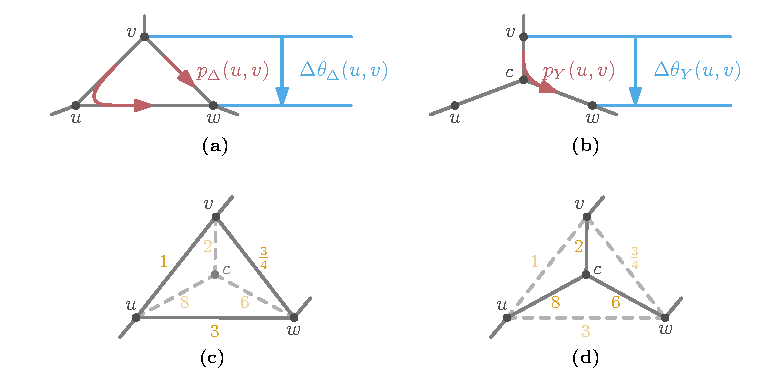
\includegraphics{networkAnalyzes/figures/Delta-Wye-Transformation.pdf}
    % 
    \caption[The delta-wye- and wye-delta-transformations.]{The delta-wye-
    (\cref{ch:network-analyzes:sec:mathematical-model:sim:deltawye_transformation})
    and wye-delta-transformations
    (\cref{ch:network-analyzes:sec:mathematical-model:sim:wyedelta_transformation})
    represent possible transformation rules in electrical networks. In this
    example, we have a graph with three (respectively four)
    vertices~\tikzStandardVertex. If we explicitly compute the susceptances we
    write the \textcolor{SUSCEPTANCE}{susceptance~\glssymbol{susceptance}} on
    each edge. (a)~The triangle~$\Delta$ can be transformed to a star~$Y$.
    Recall that we have only linear maps and work on a field~$\mathbb F$
    (here~\reals). Thus, we can superpose the paths that is a simple addition
    operation, \eg, $ (\vertexb,\vertexc)$ is equal to the series circuit
    of~$(\vertexb,\vertexa)$ and~$(\vertexa,\vertexc)$, which is parallel
    to~$(\vertexb,\vertexc)$ meaning~$
        % 
        \big(
            (\vertexb,\vertexa),
            (\vertexa,\vertexc)
        \big)
        ||
        (\vertexb,\vertexc)
        % 
    $.
    This electrical addition can be done for the \textcolor{SUSCEPTANCE}
    {susceptances~\glssymbol{susceptance}} and \textcolor{KITred70}{electrical
    (\eg, power) flows~$\glssymbol{realpower}$}. The voltage angle (potential)
    difference stays the same~$
        % 
        \textcolor{THETA}{\glssymbol{voltageangledifference}}
        % 
    $. (b)~This star~$Y$ can be transformed to a triangle~$\Delta$ and can use
    similar properties as described in~\mbox{(a)}.
    (c)~The~\deltawye-transformation increases the number of vertices by one and
    decreases the number of cycles by one. (d)~The~\wyedelta-transformation
    increases the number of cycles by one and decreases the number of vertices
    by one.}
    % 
    \label{ch:network-analyzes:sec:mathematical-model:fig:DeltaWyeTransformation}
    % 
\end{figure}
% 
The next graph transformations are more complex and were first introduced
by~\textcite{Ken99}. The~\deltawye-Transformation (also known as Delta-Wye- or
Triangle-Star-Transformation) and~\wyedelta-Transformation are inversions to
each other.
% 
\begin{reductionrule}[\deltawye-Transformation]
    % 
    Let~\vertexa, \vertexb, and~\vertexc form a complete graph with the edge
    set~$\glssymbol{undirectededges}_{\Delta}\subseteq\glssymbol{undirectededges}$
    (see~\cref{ch:network-analyzes:sec:mathematical-model:fig:DeltaWyeTransformation}\screen{a}).
    This delta~$\Delta$ can be transformed to a wye~$Y$ by adding a new
    vertex~\vertexStar representing the center of the wye~$Y$
    to~$\glssymbol{vertices}$ and new edges to the triangle's vertices~$
        % 
        \glssymbol{undirectededges}
        \cup
        \big\{
            \{\vertexStar,\vertexa\}
            \mid
            \{\vertexa,\vertexb\}
            \in
            \glssymbol{undirectededges}_{\Delta}
        \big\}
        \setminus
        \glssymbol{undirectededges}_{\Delta}
        % 
    $
    (see~\cref{ch:network-analyzes:sec:mathematical-model:fig:DeltaWyeTransformation}\screen{b}).
    % 
    \begin{subequations}
        \begin{align}
        %
        \glssymbol{susceptance}(\vertexa,\vertexStar)%
        &= 
        \frac{
            \glssymbol{susceptance}(\vertexa,\vertexb)%
            \cdot
            \glssymbol{susceptance}(\vertexa,\vertexc)%
            +
            \glssymbol{susceptance}(\vertexa,\vertexb)%
            \cdot
            \glssymbol{susceptance}(\vertexb,\vertexc)%
            +
            \glssymbol{susceptance}(\vertexa,\vertexc)%
            \cdot
            \glssymbol{susceptance}(\vertexb,\vertexc)%
        }{
            \glssymbol{susceptance}(\vertexb,\vertexc)%
        }\\%
        %
        \glssymbol{capacity}(\vertexa, \vertexStar) 
        &= 
        \glssymbol{capacity}(\vertexa,\vertexb) 
        + 
        \glssymbol{capacity}(\vertexa,\vertexc) 
        - 
        \big(%
            \glssymbol{flow}(\vertexb,\vertexStar)%
            -%
            \glssymbol{flow}(\vertexc, \vertexStar)%
        \big)%
        %
        \end{align}
    \end{subequations}
    % 
    \label{ch:network-analyzes:sec:mathematical-model:sim:deltawye_transformation}%
    % 
\end{reductionrule}
% 
The inverse rule of the~\deltawye-transformation is denoted
by~\wyedelta-Transformation.
% 
\begin{reductionrule}[\wyedelta-Transformation]
    Let~$
        % 
        \vertexStar
        \in
        \glssymbol{vertices}
        \setminus
        (\glssymbol{generators}\cup\glssymbol{consumers})
        % 
    $ be a vertex with a degree of~$\degree(\vertexStar) = 3$
    (see~\cref{ch:network-analyzes:sec:mathematical-model:fig:DeltaWyeTransformation}\screen{b}
    and~\screen{d}). Thus, vertex~\vertexStar forms the center of a wye~$Y$ with
    neighbors~\vertexa, \vertexb, and~\vertexc. The transformation of the
    wye~$Y$ results in a equivalent network that is a delta~$\Delta$ by~$
        % 
        \glssymbol{undirectededges}''
        \cup
        \big\{
            \{\vertexa,\vertexb\}
            \mid
            \{\vertexStar,\vertexa\}
            \in
            \glssymbol{undirectededges},
            \{\vertexStar,\vertexb\}
            \in
            \glssymbol{undirectededges}~\text{with}~\vertexa
            \not\eq
            \vertexb
        \big\}
        \setminus
        \big\{
            \{\vertexStar,\vertexa\}
            \in
            \glssymbol{undirectededges}
        \big\}
        % 
    $ and~$
        % 
        \glssymbol{vertices}
        \setminus
        \{\vertexStar\}
        % 
    $
    (see~\cref{ch:network-analyzes:sec:mathematical-model:fig:DeltaWyeTransformation}%
    \screen{a} and~\screen{c}) with the susceptances
    % 
    \begin{align}
        % 
        \glssymbol{susceptance}(\vertexa,\vertexb) 
        &= 
        \frac{
            \glssymbol{susceptance}(\vertexa,\vertexStar)
            \cdot
            \glssymbol{susceptance}(\vertexb,\vertexStar)
        }{
            \glssymbol{susceptance}(\vertexa,\vertexStar) 
            + 
            \glssymbol{susceptance}(\vertexb,\vertexStar) 
            + 
            \glssymbol{susceptance}(\vertexc,\vertexStar)
        }.
        % 
    \end{align}
    % 
    \label{ch:network-analyzes:sec:mathematical-model:sim:wyedelta_transformation}
    % \franzi{How to transform the capacity?}
\end{reductionrule}
% 
The basic idea of the latter transformation is that we remove a
vertex~\vertexStar that is the center of a wye~$Y$ and connect all its neighbors
by an edge. Note that the previous transformation removes a vertex from the
graph, which reduces the size of the network. The next transformation is a
generalization
of~\cref{ch:network-analyzes:sec:mathematical-model:sim:wyedelta_transformation}.

Note that a star of arbitrary degree~$\deg(\vertexStar)$, where~\vertexStar is
the center of a star, is a more general notation for wye and in this case a
\emph{polygon} is a complete graph~$K_{\deg(\vertexStar)}$ representing a
generalization of a triangle (\ie, $K_3$).
% 
% TODO: N(c) independent?
%  
\begin{reductionrule}[Star-Polygon-Transformation~{{\parencite[p.916]{Ros24}}}]
    % 
    Let~$\vertexStar\in\glssymbol{vertices}\setminus(\glssymbol{generators}\cup
    \glssymbol{consumers})$ be a vertex with a degree of~$\degree(\vertexStar)$.
    Thus, vertex~\vertexStar forms the center of a star with
    neighbors~$\neighbor(\vertexStar)$. Transforming a star into a polygon
    by~$
        % 
        \glssymbol{edges}'
        =
        \glssymbol{edges}
        \cup
        \big\{
            \{\vertexa,\vertexb\}
            \mid
            \vertexa 
            \in
            \neighbor(\vertexStar), 
            \vertexb 
            \in
            \neighbor(\vertexStar)~\text{with}~\vertexa
            \not\eq
            \vertexb
        \big\}
        \setminus
        \big\{
            \{\vertexStar,\vertexa\}
            \in
            \glssymbol{edges}
            \mid
            % \forall
            \vertexa
            \in
            \neighbor(\vertexStar)
        \big\}
        % 
    $
    and~$
        % 
        \glssymbol{vertices}' 
        = 
        \glssymbol{vertices}
        \setminus
        \{\vertexStar\}
        % 
    $, we get the susceptances
    % 
    \begin{align}
        \glssymbol{susceptance}(\vertexa,\vertexb) 
        &= 
        \frac{
        \glssymbol{susceptance}(\vertexa,\vertexStar)
        \cdot
        \glssymbol{susceptance}(\vertexb,\vertexStar)
        }{
            \sum_{
                \{\vertexa,\vertexStar\}
                \in
                \glssymbol{edges}
            }
            \glssymbol{susceptance}(\vertexa,\vertexStar)
        }
        \qquad
        \forall
        \vertexa,\vertexb
        \in
        \neighbor(\vertexStar).%
    \end{align}
    % 
    % the transformation has no general inverse without additional constraints
    % - by polygon they mean a complete graph
    % \franzi{Check: \parencite{Lie73,Bed61,CURTIS1998115}}
    % \cite{shew1947xxvii} inverse transformation under Wheatstone's condition
    \label{ch:network-analyzes:sec:mathematical-model:sim:star-polygon-transformation}
\end{reductionrule}
% 
One of the first applications is given by~\textcite{But21} on the earth capacity
effects. \textcite[p.917; Figure 3]{Ros24} calculates the effective conductance
between two terminals using the next transformation. \textcite[p.917; Figure
4]{Ros24} calculates the effect on the balance of Wheatstone bridges by the
earth admittance between two terminals using the latter transformation.% Similar
% results exist for double-bridge networks and Wagner double bridge/Wien
% bridges~\franzi{?}.

Note that if there is already an
edge~$\{\vertexa,\vertexb\}\in\glssymbol{undirectededges}$, we can apply in
addition
to~\cref{ch:network-analyzes:sec:mathematical-model:sim:star-polygon-transformation}
a parallel contraction in form
of~\cref{ch:network-analyzes:sec:mathematical-model:sim:parallel_contraction}.
We now reference two other reduction rules for the sake of completeness.
%
\begin{reductionrule}[Polygon-to-Chain-Reduction~{{\parencite{Sat85}}}]
    % 
    See~\textcite{Sat85} for more information.
    % 
    \label{ch:network-analyzes:sec:mathematical-model:sim:polygon_to_chain_reduction}
    % 
\end{reductionrule}
% 
% - \textcite{1086780} formulated an open question 
% - one \textcite{Bed61} provided a necessary relationship that takes
% the product of the admittances of the two parallel branches and equating it with
% the product of the admittances of the two diagonal branches of the
% quadrilateral
% -> sufficiency requires that every one in th edet satisfy the condition

% - Idea: Basically checks symmetry required by \textcite[p.916;(1)]{Ros24}
%
\begin{reductionrule}[Trisubgraph-Y-Reduction~{{\parencite{Sat93}}}]
    % 
    See~\textcite{Sat93} for more information.
    % 
    \label{ch:network-analyzes:sec:mathematical-model:sim:polygon_to_chain_reduction}
    % 
\end{reductionrule}
% 
We denote a graph~\glssymbol{graph} to be \emph{$k$-edge reducible} if there is
a series of application of reduction rules 
(\cref{ch:network-analyzes:sec:mathematical-model:sim:series_contraction,ch:network-analyzes:sec:mathematical-model:sim:parallel_contraction,ch:network-analyzes:sec:mathematical-model:sim:deltawye_transformation,ch:network-analyzes:sec:mathematical-model:sim:wyedelta_transformation})
such that the resulting graph has only~$k$ remaining edges.
% 
\begin{theorem}[{{\textcite{Epi66}}}]
    % 
    Every biconnected plane \source-\sink-graph with an~$(\source,\sink)$-edge
    is $1$-edge reducible.
    % 
    \label{ch:network-analyzes:sec:mathematical-model:thm:epifanov}
    % 
\end{theorem}
%
\begin{wrapfigure}{l}{4.5cm}%
    % 
    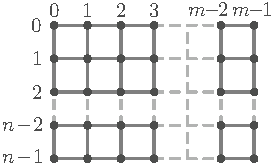
\includegraphics[scale=1,page=1]{networkAnalyzes/figures/GridGraph.pdf}
    % 
    \caption[A grid graph.]{%
    % 
    A grid graph~\glssymbol{graph} of size~$n\times m$ with~$n, m \geq 2$.
    %
    }%
    % 
    \label{ch:network-analysis:fig:grid-graph}%
    % 
\end{wrapfigure}% 
% 
\noindent To understand the next result, we define grid graphs and minors. A
(square)~\emph{grid graph}~$
    % 
    \glssymbol{graph}_{\mathrm{grid}} 
    = 
    (
    \glssymbol{vertices}_{\mathrm{grid}},
    \glssymbol{edges}_{\mathrm{grid}}
    )
    % 
$ (also known as lattice graph) is a plane graph, where each edge has unit
length and is drawn either by a horizontal or a vertical straight curve. The
grid points are crossings represented by vertices
(\cref{ch:network-analysis:fig:grid-graph}). A~\emph{minor} is a graph that can
be obtained from a graph~\glssymbol{graph} by contracting edges and by deleting
vertices and edges.

\noindent We use the following results to provide a first algorithm
for~\gls{dc}~\gls{feas} and~\gls{mpfp} on
plane~\source-\sink-graphs~\glssymbol{graph}.
%%%%%%%%%%%%%%%%%%%%%%%%%%%%%%%%%% ALGORITHM %%%%%%%%%%%%%%%%%%%%%%%%%%%%%%%%%%%
%
% \wormhole{bit:ch:switching:sec:exploit_structural_characteristics:subsec:dtp:alg:shortest_theta_path}
% \def\HiLi{\leavevmode\rlap{\hbox to \hsize{\color{HiLi}\leaders\hrule
% height .9\baselineskip depth 1.3ex\hfill}}}
\begin{algorithm}[tb!]%
\SetAlgoLined
%%%%%%%%%%%%%%%%%%%%%%%%%%%%%%%%%%
% 
\KwData{A network~\dcnetworktuple with~$\fmagnitude{\glssymbol{generators}} = 1$ (\ie,
$\{\source\} = \glssymbol{generators}$), $\fmagnitude{\glssymbol{consumers}} = 1$ 
(\ie, $\{\sink\} = \glssymbol{consumers}$), 
$\realpowergeneration = \realpowergenerationmin = \realpowergenerationmax$, 
and $\realpowerdemand = \realpowerdemandmin = \realpowerdemandmax$.}
% 
\KwResult{Flow~$\glssymbol{flow}(\vertexa,\vertexc)$ for all $
(\vertexa,\vertexc)\in\glssymbol{edges}$, flow value~$\glssymbol{flowvalue}(\glssymbol{flow},\glssymbol{network})$, and
voltage angles~$\glssymbol{voltageangle} (\vertexa)$
with~$\vertexa\in\glssymbol{vertices}$.}
% 
% INITIALIZATION %%%%%%%%%%%%%%%%%%%%%%%%%%%%%%%%%%%%%%%%%%%%%%%%%%%%%%%%%%%%
% 
$\embedding\hspace{4mm} = \algoplanarembedding(\glssymbol{graph})$
\hspace*{-1mm}%
\label{ch:network-analyzes:algo:stpf:planarEmbedding}
\Comment*{\color{KITblack30} PQ-Tree; see~\cref{ch:network-analyzes:sec:planar-embedding-dual-graph-construction}}%
% 
$\embedding_{\mathrm{grid}} 
= 
\algoGridEmbeddingOfPlanarGraph(\glssymbol{graph}(\embedding))$
\label{ch:network-analyzes:algo:stpf:gridEmbedding}
\Comment*{\color{KITblack30} see~\cref{ch:network-analyzes:sec:mathematical-model:lemma:embedding-into-a grid}}%
% 
$
\big( 
    \gls{network} = \gls{network}_0
    ,\dots
    ,\gls{network}_k 
        = \big( 
            (\{\source,\sink\}, \{\edge'\})
            , \{\source\}
            , \{\sink\}
            ,\gls{capacity}'
            ,\gls{susceptance}'
            ,\realpowergeneration
            ,\realpowerdemand) 
          \big)
\big) \allowbreak
\hspace*{5mm}= 
\algoContractGridGraphToEdge(\gls{network}(\embedding_{\mathrm{grid}}))$
\label{ch:network-analyzes:algo:stpf:contractGridGraphToEdge}%
\Comment*{\color{KITblack30} see~\cref{ch:network-analyzes:sec:mathematical-model:lem:grid-graph-deltawye-reducible}}%
$\gls{flow}(\edge') = \realpowergeneration = \realpowerdemand$
\label{ch:network-analyzes:algo:stpf:flowAssignment}%
\;
% 
$
    \glssymbol{flow}
    \hspace{5mm}=
    \algoDecontractEdgeToGridGraph((\gls{network}_0,\dots,\gls{network}_k),\flow(\edge'))
$
\label{ch:network-analyzes:algo:stpf:decontractGridGraphToEdge}%
\;
% 
$
    \gls{flow} 
    \hspace{5mm}= 
    \algoRescalePowerFlow(\gls{network},\gls{flow})$%
\label{ch:network-analyzes:algo:stpf:rescaling}%
\Comment*{\color{KITblack30} see~\cref{ch:network-analyzes:sec:mathematical-model:lem:rescalling-an-pf}}%
% 
\Return~\glssymbol{flow}\;
%
%%%%%%%%%%%%%%%%%%%%%%%%%%%%%%%%%%
%
\caption{\source-\sink Planar~\gls{dc}~\gls{feas}(\glssymbol{network})
 \&~\source-\sink Planar~\gls{mpfp}(\glssymbol{network})}
\label{ch:network-analyzes:algo:s-t-power-flow-transformation-algorithm}% 
\end{algorithm}% 
%%%%%%%%%%%%%%%%%%%%%%%%%%%%%%%%%%%%%%%%%%%%%%%%%%%%%%%%%%%%%%%%%%%%%%%%%%%%%%%%
% 
\begin{lemma}[{{\parencite[p.144; Lemma~6]{Tru89}}}]
    % 
    Every plane graph is a minor of some grid graph.
    % 
    \label{ch:network-analyzes:sec:mathematical-model:lem:plane-graph-grid-graphs}
    % 
\end{lemma}
% 
Let a grid graph~$
    % 
    \glssymbol{graph}_{\mathrm{grid}} 
    = 
    (
    \glssymbol{vertices}_{\mathrm{grid}},
    \glssymbol{edges}_{\mathrm{grid}}
    )
    % 
$ be a graph that is numbered column-wise from left to right with~$1, \dots, m$
and row-wise from top to bottom with~$1, \dots, n$
(see~\cref{ch:network-analysis:fig:grid-graph}).
% 
Similar to~\textcite{Tru89}, we define an \emph{extended grid graph}~$
\glssymbol{graph}_{\mathrm{ex}}^\ell$ as a graph on a grid with~$\ell \geq 2$, 
where~$\ell \in \naturals$ represents the number of columns and rows with~$0
\leq i \leq \ell-1$. Since the grid is quadratic, we have~$\ell^2$ vertices, and
edges connecting a vertex~$\vertex_{i,0}$ on the left border at row~$i$
% 

\begin{wrapfigure}{r}{4.25cm}%
    % 
    \vspace*{-0.75cm}
    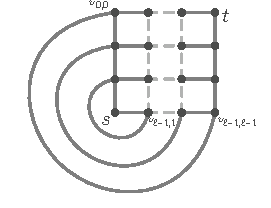
\includegraphics[scale=1,page=1]{networkAnalyzes/figures/ExtendedGridGraph.pdf}
    % 
    \caption[An extended grid graph.]{%
        % 
        An extended grid graph~$\glssymbol{graph}_{\mathrm{ex}}^\ell$ with
        a grid of dimension~$\ell\times\ell$ and~$\ell^2$ vertices.
        %
        \vspace*{-1.0cm}
    }%
    % 
    \label{ch:network-analysis:fig:extended-grid-graph}%
    % 
\end{wrapfigure}% 
% 
\noindent column~$0$ of the grid to a vertex~$\vertex_{\ell-1,i}$ on the bottom
border (see~\cref{ch:network-analysis:fig:extended-grid-graph}) such that either
the source~\source or the sink~\sink is located on the inner face
(in~\cref{ch:network-analysis:fig:extended-grid-graph} the source~\source is on
the inner face). We illustrated such a
graph~$\glssymbol{graph}_{\mathrm{ex}}^\ell$
in~\cref{ch:network-analysis:fig:extended-grid-graph}.
% 
\begin{lemma}[{{\parencite[p.145; Lemma~13]{Tru89}}}]
    % 
    Any plane graph~\glssymbol{graph} with~$(\source,\sink)\in\glssymbol{edges}$
    and with one of the two terminals (\ie, source~\source or sink~\sink) on the
    outer face, is a minor of some extended grid
    graph~$\glssymbol{graph}_{\mathrm{ex}}^\ell$ with~$\ell \geq 2$.
    % 
    \label{ch:network-analyzes:sec:mathematical-model:lem:plane-graph-grid-graphs}
    % 
\end{lemma}
% 
Note that it is always possible to use the inverse of all reduction rules
but~\cref{ch:network-analyzes:sec:mathematical-model:sim:star-polygon-transformation}.
In the following, we try to embed the graph~\glssymbol{graph} such that the
embedding has the form of an extended grid graph. We need the concept of a face
in the following
(\cref{ch:network-analyzes:sec:mathematical-model:subsec:planar-graphs}). For a
plane graph~\glssymbol{graph} a face~\cycle is a region that is bounded by the
edges and vertices of~\glssymbol{graph}. Two faces are incident if they share at
least one edge.
% 
\begin{lemma}
    % 
    Any plane \source-\sink-electrical-network~\glssymbol{network} with at least
    one terminal on the outer face can be embedded into a grid
    in~$\bigO(\fmagnitude{\glssymbol{vertices}})$ time.
    % 
    \label{ch:network-analyzes:sec:mathematical-model:lemma:embedding-into-a grid}
    % 
\end{lemma}
% 
\begin{figure}[t!]
    % 
    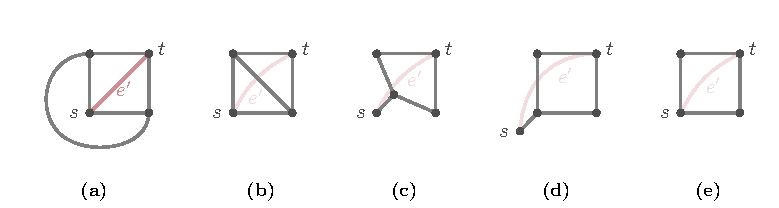
\includegraphics{networkAnalyzes/figures/Delta-Wye-Reducibility-Case-1.pdf}
    % 
    \caption[The delta-wye-reducibility of the smallest extended grid graph.]{A
    graph with four vertices, five edges, and one additional edge~$\edge' =
    (\source,\sink) \in \glssymbol{edges}$. The shown steps represent the
    reduction of the smallest possible extended grid
    graph~$\glssymbol{graph}_{\mathrm{ex}}^\ell$ with~$\ell = 2$. The steps are
    given in~\textcite{Tru89} for graphs in general. From (a) to (b) we just
    swap the outer edge to the inner face. From (b) to (c), we do a triangle to
    star transformation
    (see~\cref{ch:network-analyzes:sec:mathematical-model:sim:deltawye_transformation})
    of the lower left triangle. In the last step from (d) to (e), we do a series
    contraction
    (see~\cref{ch:network-analyzes:sec:mathematical-model:sim:series_contraction})
    and contract the edge in the bottom left with~$\edge'$. To contract the
    remaining graph to one edge~$\edge'=\{\source,\sink\}$, we do two series
    contractions and one parallel contraction.
    % 
    }
    %
    % Delta-Wye-Reducibility case 1 
    \label{ch:network-analyzes:sec:mathematical-model:fig:delta-wye-reducibility-case-1}
    % 
\end{figure}
% 
\begin{proof}
Note that the maximum degree of a grid graph~$
    % 
    \glssymbol{graph}_{\mathrm{grid}} 
    = 
    (
    \glssymbol{vertices}_{\mathrm{grid}},
    \glssymbol{edges}_{\mathrm{grid}}
    )
    % 
$ is at most~$4$. Thus, we split all vertices~$
    % 
    \vertex \in \glssymbol{vertices}(\glssymbol{graph})
    % 
$ with degree of at least~$
    % 
    \degree(\vertex)\geq 5
    % 
$. With~$\degree(\vertex)\leq 2 n_\vertex + 2$, we split them into~$
    % 
    n_\vertex 
    =
    \ceil{\nicefrac{\degree(\vertex)-2}{2}}
    =
    \ceil{\nicefrac{\degree(\vertex)}{2}}-1
    % 
$ vertices~$\vertex_i$ with $1\leq i \leq n_\vertex$ with~$
    % 
    \glssymbol{vertices}_{\vertex} 
    \coloneqq
    \left\{
        % \bigcup_{1\leq i \leq n_\vertex}
        \vertex_i
        \mid
        1\leq i \leq n_\vertex,
        \vertex\in\glssymbol{vertices} \colon
        \degree(\vertex) \geq 5
    \right\}
    % 
$ such that~$
    % 
    \glssymbol{vertices}_{\mathrm{grid}} 
    = 
    % \left\{
        \bigcup_{
            \{
                \vertex
                \in
                \glssymbol{vertices}
                \mid
                \degree(\vertex) \geq 5
            \}
        }
        \glssymbol{vertices}_{\vertex} 
    \cup
    \left(
        \glssymbol{vertices}(\glssymbol{graph})
        \setminus
        \{\vertex\}
    \right)
    % 
$ and~$
    % 
    \glssymbol{edges}_{\mathrm{grid}} 
    = 
    \glssymbol{edges}(\glssymbol{graph})
    \cup
    \big\{
        \{\vertex_i, \vertex_{i+1}\}
        \mid
        \vertex_i, \vertex_{i+1}\in\glssymbol{vertices}_{\vertex},
        \forall
        \vertex
        \in
        \glssymbol{vertices}_{\mathrm{grid}} 
        \setminus
        \glssymbol{vertices}(\glssymbol{graph})
    \big\}
    % 
$ with susceptance~$
    % 
    \glssymbol{susceptance}(\edge)
    =
    \infty
    % 
$ with~$
    % 
    \edge
    \in
    \glssymbol{edges}_{\mathrm{grid}}
    \setminus
    \glssymbol{edges}(\glssymbol{graph})
    % 
$. We set the susceptance to infinity such that~$
    % 
    \glssymbol{voltageangledifference}(\vertex_i,\vertex_{i+1})
    =
    \nicefrac{
        \glssymbol{flow}(\vertex_i,\vertex_{i+1})
    }{
        \glssymbol{susceptance}(\vertex_i,\vertex_{i+1})
    }
    =
    \nicefrac{
        \glssymbol{flow}(\vertex_i,\vertex_{i+1})
    }{
        \infty
    }
    \approx
    0
    % 
$ meaning that the voltage angles~$\glssymbol{voltageangle}(\vertex_i)$ are the
same for all~$\vertex_i\in\glssymbol{vertices}_{\vertex}$ with~$1\leq i\leq
n_{\vertex}$. Since the average degree of a finite plane graph is strictly less
than~$6$, we get~$2$ new vertices per vertex on average and thus, we
have~$\bigO(\fmagnitude{\glssymbol{vertices}})$ vertices.

Assume an arbitrary planar embedding of~$\glssymbol{graph}_{\mathrm{grid}}$.
Thus, we choose an inner face~$\cycle_{\source_1}$ that is incident to the
vertex~\source and choose a cut in the dual graph~$S\subseteq\glssymbol{edges}$
between~$\cycle_{\source_1}$ and the outer face~$\cycle_{o}$. Let~$
    % 
    \glssymbol{graph}_{\mathrm{grid}}' 
    =
    (
        \glssymbol{vertices}_{\mathrm{grid}}',
        \glssymbol{edges}_{\mathrm{grid}}'
    )
    % 
$ be a new graph with vertex set~$
    % 
    \glssymbol{vertices}' 
    =
    \glssymbol{vertices}
    \cup
    \{\source'\}
    % 
$ and edge set~$
    % 
    \glssymbol{edges}(\glssymbol{graph}') 
    =
    \glssymbol{edges}(\glssymbol{graph})
    \cup
    \big\{
        \{\source,\source'\}
    \big\}
    \setminus 
    S
    % 
$ with~$\glssymbol{susceptance} (\source,\source') = \infty$. This graph can be
embedded in~$
    % 
    \bigO(
        \fmagnitude{\glssymbol{vertices}}
    )
    % 
$ time into a grid of size at
most~$
    % 
    \fmagnitude{\glssymbol{vertices}}
    \times
    \fmagnitude{\glssymbol{vertices}}
    % 
$ using, \eg, the algorithm of~\textcite{Bie98}. Thus, we need~$
    % 
    \bigO(\fmagnitude{\glssymbol{vertices}}^2)
    % 
$ space.
This takes~$\bigO(\fmagnitude{\glssymbol{vertices}})$ time.
% 
\end{proof}
% 
% -Sch\"affter showed that is possible to draw any graph onto a~$2n\times 2n$ grid
% with at most 2 bends per edge "Drawing graphs on rectangular grids"
% - graphs with max degree 3 can be embedded in an 
% % $\ceil{\frac{n}{2}}\times\ceil{\frac{n}{2}}$ grid with~$\ceil{\frac{n}{2}}+2$ bends
% if the graph is planar it can be embedded in an $n\times n$ grid with $2n+4$
% bends if biconnected and $2.4n+2$ bends otherwise [23,25]
% - choose an arbitrary planar embedding of \glssymbol{graph}
% - choose an incident face of t as outer-face
% - choose a vertex s not = t on the outer-face
% - obtain a st-ordering
% 
We note that the outer edges that make the grid graph into an extended grid
graph
can be added by applying the following steps: 
% 
We add the remaining edges in~$S$. We place~$\source'$ on the bottom left
corner. Each time we add an edge~$
    % 
    \{\vertexa,\vertexb\}
    \in
    \glssymbol{undirectededges}
    % 
$ we check if~$\vertexa_{i_{\vertexa},0} = \vertexb_{\ell-1,i_{\vertexb}}$. If
neither is true then we add~$i_{\vertexb} - i_{\vertexa}$ new rows 
if~$i_{\vertexa}<i_{\vertexb}$ or new columns if~$i_{\vertexb}<i_{\vertexa}$.

Every plane electrical network can be embedded into a grid by using the
aforementioned algorithm. Thus, we make use of the following lemma.
% 
\begin{lemma}[{{\parencite[pp.142ff.; Theorem~2 \& Lemma~14]{Tru89}}}]
    % 
    Every (extended) grid graph with one source and one sink is 1-edge
    reducible.
    % 
    \label{ch:network-analyzes:sec:mathematical-model:lem:grid-graph-deltawye-reducible}
    % 
\end{lemma}
% 
So far we explained the different parts of the algorithm. Note that we assume a
plane~\source-\sink-graph~\glssymbol{graph} for the
algorithm. The algorithm (see~\cref{ch:network-analyzes:algo:s-t-power-flow-transformation-algorithm}) works as follows.
From~\cref{ch:network-analyzes:sec:mathematical-model:lemma:embedding-into-a
grid,ch:network-analyzes:sec:mathematical-model:lem:grid-graph-deltawye-reducible},
we know that any plane graph can be embedded into a grid
(see~\cref{ch:network-analyzes:algo:s-t-power-flow-transformation-algorithm}~\cref{ch:network-analyzes:algo:stpf:gridEmbedding})
and that every grid graph can be contracted to a single edge~$\edge'$
(see~\cref{ch:network-analyzes:algo:s-t-power-flow-transformation-algorithm}~\cref{ch:network-analyzes:algo:stpf:contractGridGraphToEdge}
and~\cref{ch:network-analyzes:sec:mathematical-model:fig:delta-wye-reducibility-case-1}).
In each~\deltawye-reduction, we compute the susceptances by the aforementioned
rules
(see~\cref{ch:network-analyzes:sec:mathematical-model:sim:deltawye_transformation,ch:network-analyzes:sec:mathematical-model:sim:wyedelta_transformation}).
% 
In the decontraction step
(see~\cref{ch:network-analyzes:algo:s-t-power-flow-transformation-algorithm}~\cref{ch:network-analyzes:algo:stpf:decontractGridGraphToEdge}),
we compute based on the given susceptances on the different contraction levels
the voltage angles~$\gls{voltageangle}(\vertexa)$
with~$\vertexa\in\gls{vertices}_i$ and the flow for each contraction level~$i$.
We start with~$\gls{network}_k$ consisting of a single edge~$\edge'$,
over~$\gls{network}_{k-1}$, and in the end we compute the voltage angles and the
flow for the original network~$\gls{network}_0$. For each level transition, we
apply the reverse of the applied transformation rules given
in~\cref{ch:network-analyzes:sec:mathematical-model:sim:series_contraction,ch:network-analyzes:sec:mathematical-model:sim:parallel_contraction,ch:network-analyzes:sec:mathematical-model:sim:loop_contraction,ch:network-analyzes:sec:mathematical-model:sim:degree_1_contraction,ch:network-analyzes:sec:mathematical-model:sim:deltawye_transformation,ch:network-analyzes:sec:mathematical-model:sim:wyedelta_transformation}.
% 
Note from~\cref{ch:network-analyzes:sec:mathematical-model:lem:rescalling-an-pf}
on 
Page~\pageref{ch:network-analyzes:sec:mathematical-model:lem:rescalling-an-pf}
that the capacities can be neglected, since we are always able to rescale a 
nontrivial electrical flow. This rescaling is not necessary
for~\gls{dc}~\gls{feas}, since a capacity violation would imply a non-existing
feasible electrical flow. However, assume that we apply an arbitrary flow
on~$\edge'$
(see~\cref{ch:network-analyzes:algo:s-t-power-flow-transformation-algorithm}~\cref{ch:network-analyzes:algo:stpf:flowAssignment})
resulting in an electrical flow that is not necessarily feasible, since the
capacity constraint might be violated. To fix the violation, we
use~\cref{ch:network-analyzes:sec:mathematical-model:lem:rescalling-to-mpf} on
Page~\pageref{ch:network-analyzes:sec:mathematical-model:lem:rescalling-to-mpf}
on the decontracted graph~\glssymbol{graph} with flow~\glssymbol{flow} to
rescale the flow to a feasible, \eg~\gls{mpf} 
(see~\cref{ch:network-analyzes:algo:s-t-power-flow-transformation-algorithm}~\cref{ch:network-analyzes:algo:stpf:rescaling}).
From~\textcite{Tru89}, we get the following running time.
% 
\begin{figure}[t!]
    % 
    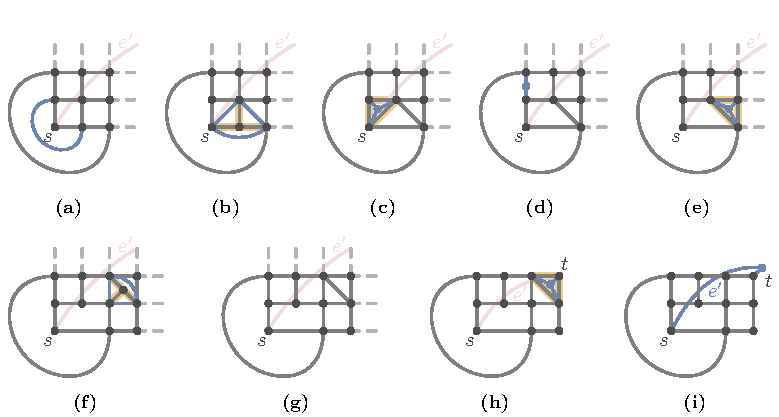
\includegraphics{networkAnalyzes/figures/Delta-Wye-Reducibility-Case-2.pdf}
    % 
    \caption[The delta-wye-reducibility of a general extended grid graph.]{A
    general extended grid graph~$\glssymbol{graph}_{\mathrm{ex}}^\ell$
    with~$\ell^2$ vertices. Blue edges and blue vertices represent the edges and
    vertices of the transformation and replace the orange marked edges. The
    steps are basically given by~\textcite{Tru89} for graphs in general. From
    (a) to (b) we use the steps already shown
    in~\cref{ch:network-analyzes:sec:mathematical-model:fig:delta-wye-reducibility-case-1}.
    % 
    }    % Delta-Wye-Reducibility case 2
    \label{ch:network-analyzes:sec:mathematical-model:fig:delta-wye-reducibility-case-2}
    % 
\end{figure}

\begin{lemma}
    % 
    The algorithm runs in~$\bigO(\fmagnitude{\glssymbol{vertices}}^3)$ time. 
    % and
    % needs~$\bigO(\fmagnitude{\glssymbol{vertices}}^2)$ space.
    % 
    \label{ch:network-analyzes:sec:mathematical-model:obs:arbitrary-capacities}
    % 
\end{lemma}
% 
% Algo decontraction notes:\\
% - note that the voltage angles in a parallel decontraction stay the same as the
% edge itself\\
% - In a series contraction however these angles do not change either, but the
% inner vertices get a voltage angle between the outer ones\\
% - the voltage angles at the triangle vertices stay the same in
% \deltawye-contraction and thus \wyedelta-decontraction do not change voltage
% angles at all\\
% - in the \wyedelta-contraction and thus, \deltawye-decontraction we have to
% calculate the center new, but in  single-source and single-sink graphs the
% voltage angle is equivalent to one of the triangle ones, since the flow is
% zero\\
The contraction step of the
algorithm~\cref{ch:network-analyzes:algo:s-t-power-flow-transformation-algorithm}~\cref{ch:network-analyzes:algo:stpf:contractGridGraphToEdge}
is illustrated
in~\cref{ch:network-analyzes:sec:mathematical-model:fig:delta-wye-reducibility-case-1,ch:network-analyzes:sec:mathematical-model:fig:delta-wye-reducibility-case-2}
for an extended grid graph.
% 
\begin{lemma}
    A planar~\source-\sink-graph~\glssymbol{graph} can always be contracted to one
    edge by a series of reduction rules (see~\parencite{Tru89}).
    % 
    \label{ch:network-analyzes:sec:mathematical-model:con:planar-graph-single-edge}
\end{lemma}
% 
For the reverse operation, we remark that the voltage angles in a parallel and
series contraction do not change. For the series contraction, we have to compute
the voltage angles for the inner vertices
using~\cref{ch:network-analyzes:sec:mathematical-model:eq:kvl-ohm-function-writing}.
For the~\deltawye- and~\wyedelta-transformation, the voltage angles at the three
outer vertices do not change. For the center of the star, we have to compute the
voltage angle
using~\cref{ch:network-analyzes:sec:mathematical-model:eq:kvl-ohm-function-writing}.
The reconstruction steps can be done during the recursive return. If the
capacities are violated, we rescale the flow~\glssymbol{flow}
using~\cref{ch:network-analyzes:sec:mathematical-model:lem:rescalling-an-pf}.
From the previous discussion follows the next theorem.
% 
\begin{theorem}
    The algorithm computes a feasible electrical flow for a
    planar~\source-\sink-graph~\glssymbol{graph}.
    % 
    \label{ch:network-analyzes:sec:mathematical-model:thm:algo-pf-1}
\end{theorem}
% 
% \franzi{Cholesky Factorization}
% \franzi{Conjugate Gradient and Precondioned Conjugate Gradient -> Improve
% Preconditioners by using the structure from this and the section before }
% \franzi{
%     * We can probably improve the bounds for linear solvers, since we know what preconditioners they would like to have
%     * They use as preconditioners minimum fundamental weighted bases. 
%     * From the structure we observed in the beginning, we know that the fundamental is not necessary. 
%     * Thus, we do not need to solve an NP-hard problem, but one that is easy to solve and where polynomial time algorithm exist such as Horton and the improvements from Mehlhorn.
% }
% 
%%%%%%%%%%%%%%%%%%%%%%%%%%%%%%%%%%%%%%%%%%%%%%%%%%%%%%%%%%%%%%%%%%%%%%%%%%%%%%%
\section{Representations and Formulations of Electrical Flows}
\label{ch:network-analyzes:sec:representations}
%%%%%%%%%%%%%%%%%%%%%%%%%%%%%%%%%%%%%%%%%%%%%%%%%%%%%%%%%%%%%%%%%%%%%%%%%%%%%%%
% 
\textcite[p.13]{Cai12} mention that power grids are planar
(see~\cref{ch:network-analyzes:sec:mathematical-model:subsec:planar-graphs}) and
undirected. Recall from~\cref{ch:foundations:sec:graph-theory} that we can
transform any undirected graph to a directed graph, which we do for notational
conveniences. The planarity of graph~\glssymbol{graph} is a crucial property of
the network~\glssymbol{network} for this section. In addition, we assume that
the graph~\glssymbol{graph} is biconnected.
% 
%%%%%%%%%%%%%%%%%%%%%%%%%%%%%%%%%%%%%%%%%%%%%%%%%%%%%%%%%%%%%%%%%%%%%%%%%%%%%%%% 
\subsection{The Duality Concept for Graphs}
\label{ch:network-analyzes:sec:duality-concept}
%%%%%%%%%%%%%%%%%%%%%%%%%%%%%%%%%%%%%%%%%%%%%%%%%%%%%%%%%%%%%%%%%%%%%%%%%%%%%%%%
% 
Using the duality of the incidence matrix~\glssymbol{incidenceMatrix} and
circuit matrix~\glssymbol{cycleMatrix} that was shown
in~\cref{ch:network-analyzes:sec:mathematical-model:subsec:matroids-independence-systems},
we translate the algebraic duality of the two matrices into a graph theoretical
duality
(\cref{ch:network-analyzes:sec:mathematical-model:subsec:planar-graphs}). Recall
that a base of a
matroid~(see~\cref{ch:network-analyzes:sec:mathematical-model:def:base}) is a
maximum independent set. The complement of a base in the primal
graph~\glssymbol{graph} is the base in the dual graph~\glssymbol{dualgraph}
(see~\cref{ch:network-analyzes:sec:mathematical-model:cor:incidence-circuit-matrix-duals}).
% 
\begin{theorem}[{{\parencite[p.522; Theorem 23]{Whi35}}}]
    % 
    Let~$\glssymbol{embedding}$ be a planar embedding of a
    graph~\glssymbol{graph}. The graphs~\glssymbol{graph}
    and~\glssymbol{dualgraph} are duals if and only if there is a bijection~$
        % 
        \oneToOneMap
        \colon
        \glssymbol{edges}(\glssymbol{graph}) 
        \to
        \glssymbol{edges}(\glssymbol{dualgraph})
        % 
    $ between their edges such that bases in one correspond to base complements
    in the other.
    % 
    \label{ch:network-analyzes:sec:mathematical-model:thm:Matroids-one-to-one-corrspondence}
    % 
\end{theorem}
% 
The construction
in~\cref{ch:network-analyzes:sec:mathematical-model:subsec:planar-graphs}
implies a bijection of edges in the primal graph~\glssymbol{graph} to edges in
its dual graph~\glssymbol{dualgraph}.
% 
It is called a combinatorial dual in terms of the Whitney duality (bijection of
edges; and a set of edges forming a cut corresponds to a cycle
in the combinatorial dual). Note that the dual of a dual
graph~\glssymbol{dualgraph} is isomorphic to the primal graph~\gls{graph} as
long as~\glssymbol{graph} is connected.

From~\crefrange{ch:network-analyzes:sec:mathematical-model:eq:KCL-intermediate-vertex}{ch:network-analyzes:sec:mathematical-model:eq:KCL-consumer-vertex}, we know
that a feasible~\gls{kcl} flow on the primal graph~\gls{graph} is equivalent to
a graph theoretical flow in the primal graph~\gls{graph}.
% 
It follows
from~\cref{ch:network-analyzes:sec:mathematical-model:cor:incidence-circuit-matrix-duals}
that a feasible~\gls{kvl} flow corresponds to a graph theoretical flow in the
dual graph. Thus, we get the following lemma.
% 
\begin{lemma}
    % 
    A feasible~\gls{kvl} flow~$\glssymbol{flow}_{\glssymbol{graph}}$ in the
    primal graph~\glssymbol{graph} is equivalent to a feasible~\gls{kcl}
    flow~$\glssymbol{flow}_{\glssymbol{dualgraph}}$ in the corresponding dual
    graph~\glssymbol{dualgraph}.
    % 
    \label{ch:network-analyzes:sec:mathematical-model:lem:KVL-flow-in-dual}
    % 
\end{lemma}
% 
Note that we can apply any flow~\glssymbol{flow} on a self-loop~$
    % 
    \edge 
    =
    (\vertexa,\vertexa)
    % 
$, since it is redundant. Thus, we get the following observation.
% 
\begin{observation}
    % 
    Let the primal graph~\glssymbol{graph} be a tree. Thus, there is only one
    face that is equivalent to the outer-face~$\cycle_t$. The dual graph
    consists of self-loops only. Let~\glssymbol{flow} be any feasible flow
    on~\glssymbol{graph}. Then, flow~\glssymbol{flow} is also a feasible
    electrical flow.
    % 
    \label{ch:network-analyzes:sec:mathematical-model:eq:bnorm}
    % 
\end{observation}
%
Recall from~\cref{ch:network-analyzes:sec:reduction-transformation-rules} that
every self-loop can be removed
(see~\cref{ch:network-analyzes:sec:mathematical-model:sim:loop_contraction}).
The aforementioned observation is a geometrical explanation for planar graphs of
the results of~\textcite[p.9; Lemma 4]{Leh15a} and~\textcite{Lei15b} that on
trees any graph-theoretical flow is also electrical feasible.

We note that a series contraction
(see~\cref{ch:network-analyzes:sec:mathematical-model:sim:series_contraction})
in~\glssymbol{graph} is an equivalent transformation to the parallel contraction
(see~\cref{ch:network-analyzes:sec:mathematical-model:sim:parallel_contraction})
in the dual graph~\glssymbol{dualgraph}. We highlight that by the following
structural observation.
% 
\begin{observation}
    The series contraction in the primal graph~\glssymbol{graph} is equivalent to the parallel
    contraction in its dual~\glssymbol{dualgraph} and vice versa.
    \label{ch:network-analyzes:sec:mathematical-model:obs:parallel-series-duality}
\end{observation}
% 
\begin{observation}
    The~\deltawye-transformation in the primal graph~\glssymbol{graph} is equivalent to
    the~\wyedelta-transformation in the dual graph~\glssymbol{dualgraph} and
    vice versa.
    \label{ch:network-analyzes:sec:mathematical-model:obs:deltawye-wyedelta-duality}
\end{observation}
% 
In the following section, we will make use of the duality by reformulating the
problem.
% 
%%%%%%%%%%%%%%%%%%%%%%%%%%%%%%%%%%%%%%%%%%%%%%%%%%%%%%%%%%%%%%%%%%%%%%%%%%%%%%%%
% 
\begin{figure}[t!]
    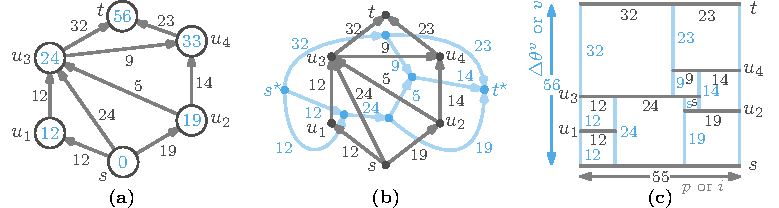
\includegraphics[page=1]{networkAnalyzes/figures/AnalogiesFlowDualSquares.pdf}
    % 
    \caption[Different representation for the power flow feasibility problem.]
    {We use the example graph of~\textcite[p.18]{Fel13}. The susceptances
    are~$\textcolor{SUSCEPTANCE}{\glssymbol{susceptance} \equiv 1}$, the
    feasible electrical flow~$\textcolor{PRIMALGRAPH}{\glssymbol{flow}(\edge)}$
    is written on each edge~$\edge\in\glssymbol{edges}$, and we neglect the
    capacities meaning~$\textcolor{CAPACITY}{\glssymbol{capacity}\equiv\infty}$.
    (a) The example graph's feasible electrical flow is in this case the minimum
    integer feasible electrical flow~\textcolor{PRIMALGRAPH}{\glssymbol{flow}}
    and the corresponding voltage
    angles~\textcolor{THETA}{\glssymbol{voltageangle}}. (b) The
    flow~\textcolor{PRIMALGRAPH}{\glssymbol{flow}} and the voltage angle
    differences~\textcolor{THETA}{\glssymbol{voltageangledifference}} can be
    separated into two graphs, which are the primal graph~\textcolor{KITblack50}
    {\glssymbol{graph}} and its dual
    graph~\textcolor{DUALGRAPH}{\glssymbol{dualgraph}}, respectively. (c) Since
    the susceptances are~$\textcolor{SUSCEPTANCE}{\glssymbol{susceptance} \equiv
    1}$ a similar representation is a squaring of
    a~$\textcolor{PRIMALGRAPH}{55}\times\textcolor{DUALGRAPH}{56}$ rectangle,
    where the \textcolor{PRIMALGRAPH}{width} and the
    \textcolor{DUALGRAPH}{height} of each square is represented by the flow in
    the \textcolor{PRIMALGRAPH}{primal} and \textcolor{DUALGRAPH}{dual graph},
    respectively. Each vertex in the \textcolor{PRIMALGRAPH}{primal} and
    \textcolor{DUALGRAPH}{dual graph} represents a
    \textcolor{PRIMALGRAPH}{horizontal} or \textcolor{DUALGRAPH}{vertical
    segment}, respectively. For clarity we labeled the vertices for the primal
    graph only, since otherwise this figure seems overloaded. An edge represents
    a side of a square. }
    % 
    \label{ch:network-analyzes:fig:AnalogiesFlowDualSquares}
    % 
\end{figure}
% 
% 
%%%%%%%%%%%%%%%%%%%%%%%%%%%%%%%%%%%%%%%%%%%%%%%%%%%%%%%%%%%%%%%%%%%%%%%%%%%%%%%% 
\subsection{Simultaneous Flow Representation}
\label{ch:network-analyzes:simultaneous-flow-representation}
%%%%%%%%%%%%%%%%%%%%%%%%%%%%%%%%%%%%%%%%%%%%%%%%%%%%%%%%%%%%%%%%%%%%%%%%%%%%%%%%
% 
We use the aforementioned duality and structure of the problem to
reformulate~\gls{dc}~\gls{feas} in terms of the~\emph{\acrlong{sfp}}
(\gls{sfp}). For~\gls{sfp} the graphs are not necessarily duals, but share some
edges.
% 
\begingroup
    %%%%%%%%%%%%%%%%%%%%%%%%%%%%%%%%%%% Problem %%%%%%%%%%%%%%%%%%%%%%%%%%%%%%%%%%%%
\begin{problem}[framed]{
% 
\acrlong{sfp}~\footnote{After showing our results to Guido Br\"uckner, he
mentioned the~\gls{sfp} generalization to us. We would like to thank him for
that generalization of the biconnected
planar~\source-\sink-\gls{dc}~\gls{feas}-problem.}~$\gls{sfp}(
\glssymbol{network})$
% 
}%
% 
% 
  Instance: & Two graphs~$\glssymbol{graph}_1$ and~$\glssymbol{graph}_2$,
  subsets $
    % 
    \glssymbol{edges}_1
    \subseteq
    \glssymbol{edges}(\glssymbol{graph}_1)
    % 
  $ and~$
    % 
    \glssymbol{edges}_2
    \subseteq
    \glssymbol{edges}(\glssymbol{graph}_2)
    % 
  $, and a bijection~$
    % 
    % \oneToOneMap
    \foneToOneMap{\gls{sfp}}
    \colon 
    \glssymbol{edges}_1 
    \to
    \glssymbol{edges}_2$.
  % 
  \\
  % 
  Question: & Are there nonzero~\gls{kcl}-feasible flows~$
    % 
    \glssymbol{flow}_{\glssymbol{graph}_1}
    % 
  $ and~$
    % 
    \glssymbol{flow}_{\glssymbol{graph}_2}
    % 
  $ in~$\glssymbol{graph}_1$ and~$\glssymbol{graph}_2$  
  % 
  % with~$\glssymbol{flowvalue}(\glssymbol{graph}_1)\not=0$ and~$
  % \glssymbol{flowvalue}(\glssymbol{graph}_2)\not=0$ 
  %  
  such that for every edge~$\edge\in\glssymbol{edges}_1$ we have~$
    % 
    \glssymbol{flow}_{\glssymbol{graph}_1}(\edge) 
    =
    \glssymbol{flow}_{\glssymbol{graph}_2}(\foneToOneMap{\gls{sfp}}(\edge))
    % 
  $?
\end{problem}%
%%%%%%%%%%%%%%%%%%%%%%%%%%%%%%%%%%%%%%%%%%%%%%%%%%%%%%%%%%%%%%%%%%%%%%%%%%%%%%%%
    \label{ch:networkAnalysis:problems:SimultaneousFlowProblem-Decision_Problem}
\endgroup
%
The reformulation of~\gls{dc}~\gls{feas} separates the
constraints---meaning~\gls{kcl} and~\gls{kvl}---by the usage of two graphs,
which we define in the following. Recall that our graph is planar and
biconnected, and that we denote by~$\oneToOneMap\colon \glssymbol{edges}
(\glssymbol{graph}(\glssymbol{embedding}))\to \glssymbol{edges}(
\glssymbol{dualgraph})$ the bijection of the edges
with~$\edge_i\mapsto\oneToOneMap(\edge_i) = \edge_i^\star$. An
edge~$(\vertexa,\vertexc) = \edge_i \in\glssymbol{graph}$ corresponds to an edge
$(\cycle_1,\cycle_2)=\edge_i^\star\in\glssymbol{dualgraph}$ and vice versa if
and only if $\edge_i$ is incident to both faces~$\cycle_1$ and~$\cycle_2$, and
$\edge_i^\star$ is incident to the faces~\vertexa and~\vertexc. Since there is
no unique embedding of a biconnected planar graph the mapping is not unique.
This means that the bijection is always related to some planar embedding of
graph~\glssymbol{graph}.

Without loss of generality, we assume that flow~$\glssymbol{flow}$ is a
function~$\glssymbol{flow}\colon\glssymbol{edges}\to\integers$. Recall that we
can always rescale~\glssymbol{flow} to a feasible electrical flow that is
non-integral (meaning~$\glssymbol{flow}\colon\glssymbol{edges}\to\reals$) by
using the scaling
from~\cref{ch:network-analyzes:sec:mathematical-model:lem:rescalling-an-pf}.

From~\cref{ch:network-analyzes:sec:mathematical-model:thm:matrix-and-its-circuit-matrix-are-duals},
we know that a graph's base of the incidence matrix and the corresponding base
of the circuit matrix are duals. Given a graph and its dual, we know
from~\cref{ch:network-analyzes:sec:mathematical-model:cor:incidence-circuit-matrix-duals}
that the incidence matrix of either graphs is equivalent to the circuit matrix
of the other, whereby equivalent means here that an edge-cut at a vertex in one
graph represents a simple cycle in the other graph and vice versa. The latter
means that for a spanning tree~\tree in graph~\glssymbol{graph} the set~$
    % 
    \glssymbol{edges}' 
    = 
    \glssymbol{edges}(\glssymbol{graph})
    \setminus
    \glssymbol{edges}(\tree)
    % 
$ of chords in one graph corresponds to a set~$
    \glssymbol{edges}'' 
    =
    \{
        \oneToOneMap(\edge)
        \mid
        \edge
        \in
        \glssymbol{edges}'
    \}
    % 
$ of edges in the dual graph, where~$\glssymbol{edges}''$ constitutes a tree.
Now,
\cref{ch:network-analyzes:sec:mathematical-model:thm:Matroids-one-to-one-corrspondence}
and~\cref{ch:network-analyzes:sec:mathematical-model:lem:KVL-flow-in-dual} can
be used to transform~\gls{dc}~\gls{feas} in terms of simultaneous flows. An edge
cut~\glssymbol{cuts} at vertex~$
% 
\vertexa
\in
\glssymbol{vertices}(\glssymbol{dualgraph})
% 
$ with~$
% 
\glssymbol{cuts}(\vertexa)
=
\{
    \edge
    \in
    \glssymbol{undirectededges}(\glssymbol{dualgraph})
    \mid
    \vertexa
    \in
    \edge
\}
% 
$ is a cycle~\glssymbol{cycle} in the biconnected planar
graph~$\glssymbol{graph}$. A conservation of flow at~\vertexa means that the
incoming flow is equivalent to the outgoing flow. For the corresponding
cycle~\glssymbol{cycle} this means that flows along the cycle sum up to zero.
Note that a flow direction in~\glssymbol{graph} corresponds to a flow direction
in~\glssymbol{dualgraph} and vice versa.

The following problem is equivalent to~\gls{dc}~\gls{feas} on~\source-\sink
plane graphs.
%
\begingroup
    %%%%%%%%%%%%%%%%%%%%%%%%%%%%%%%%%%% Problem %%%%%%%%%%%%%%%%%%%%%%%%%%%%%%%%%%%%
\begin{problem}[framed]{\source-\sink Planar~\gls{dc}~\gls{feas}(\glssymbol{network})
 % \&~\source-\sink Planar~\gls{mpfp}(\glssymbol{network}) 
 % 
 % $\source-\sink P~\gls{dc}~\gls{feas}(\glssymbol{network})$
 % $\source-\sink P~\gls{mpfp}(\glssymbol{network})$
 % 
 }%
  Instance: & A plane~\source-\sink-graph~\glssymbol{graph}, its
  dual graph~\glssymbol{dualgraph}, and the corresponding
  bijection~$\oneToOneMap\colon \glssymbol{edges}(\glssymbol{graph}) \to
  \glssymbol{edges}(\glssymbol{dualgraph})$.
  \\
  % 
  Question: & Are there simultaneous flows on~\glssymbol{graph}
  and~\glssymbol{dualgraph} such that~$
  % 
  \glssymbol{flow}_{\glssymbol{graph}}(\edge) 
  = 
  \glssymbol{flow}_{\glssymbol{dualgraph}}
  \big(
    \oneToOneMap(\edge)
  \big)
  \cdot
  \glssymbol{susceptance}(\edge)
  % 
  $ for all~$\edge\in\glssymbol{edges}(\glssymbol{graph})$?
\end{problem}%
    \label{ch:networkAnalysis:problems:DC_FEAS_simultaneous_flow-Decision_Problem}
\endgroup
% 
In the objective of the reformulated \source-\sink planar~\gls{dc}~\gls{feas}
and~\gls{dc}~\gls{mpfp}, we can easily see that this is a restatement
of~\cref{ch:network-analyzes:sec:mathematical-model:eq:kvl-ohm-function-writing}
by replacing the phase angle difference~$\glssymbol{voltageangledifference}
(\vertexa,\vertexc)\coloneqq\glssymbol{voltageangle}(\vertexc)-
\glssymbol{voltageangle}(\vertexa)$ with the flow in the dual
graph~$\glssymbol{flow}_{\glssymbol{dualgraph}}(\oneToOneMap(\edge))$ with~$\edge =
(\vertexa,\vertexc)\in\glssymbol{edges}$. An example for the reformulation is
given in~\cref{ch:network-analyzes:fig:AnalogiesFlowDualSquares}\screen{b}.
In~\cref{ch:network-analyzes:fig:AnalogiesFlowDualSquares}\screen{a}
and~\screen{b} an electrical flow with its unique voltage angle assignment and
its translation to simultaneous flows is shown, respectively. Using simultaneous
flows~\cref{ch:network-analyzes:sec:mathematical-model:eq:kvl-ohm-function-writing}
becomes~\cref{ch:network-analyzes:eq:KVL-reformulation}.
% 
\begin{equation}
    \glssymbol{flow}_{\glssymbol{graph}}(\edge) 
    =
    \glssymbol{flow}_{\glssymbol{dualgraph}} 
    \big(\oneToOneMap(\edge)\big)
    \cdot
    \glssymbol{susceptance}(\edge)
    % 
    \qquad\qquad
    \forall \edge \in \glssymbol{edges}
    % 
    \label{ch:network-analyzes:eq:KVL-reformulation}
\end{equation}
% 
Roughly speaking, the susceptance~\glssymbol{susceptance} represents a gear
ratio between the primal graph's flow~$\glssymbol{flow}_{\glssymbol{graph}}$ and
the dual graph's flow~$\glssymbol{flow}_{\glssymbol{dualgraph}}$. 
% 
\begin{theorem}
    A flow~\glssymbol{flow} in~\glssymbol{graph} is an electrical flow if and
    only if the primal flow~$\glssymbol{flow}_{
    \glssymbol{graph}}\equiv\glssymbol{flow}$ and the
    flow~$\glssymbol{flow}_{\glssymbol{dualgraph}}$ in the dual
    graph~\glssymbol{dualgraph} comply the flow conservation (\gls{kcl}) and if
    for every edge~$\edge\in\glssymbol{edges}$ the flow
    complies~$\glssymbol{flow}_{\glssymbol{graph}}(\edge) =
    \glssymbol{flow}_{\glssymbol{dualgraph}}\big(\oneToOneMap
    (\edge)\big)\cdot\glssymbol{susceptance}(\edge)$.
    % 
    \label{ch:network-analyzes:thm:electrical-flow-based-definition}
\end{theorem}
% 
\begin{proof}
    The left-hand side
    of~\cref{ch:network-analyzes:thm:electrical-flow-based-definition:1}
    and~\cref{ch:network-analyzes:thm:electrical-flow-based-definition:2} comes
    from~\cref{ch:network-analyzes:sec:mathematical-model:eq:kcl-matrix-writing}
    and~\cref{ch:network-analyzes:sec:mathematical-model:eq:kvl-matrix-writing},
    respectively. Recall that we can
    reformulate~\cref{ch:network-analyzes:sec:mathematical-model:eq:kvl-matrix-writing}
    with~$
        % 
        \glssymbol{cycleMatrix}(\glssymbol{graph})
        \cdot
        \vv{\glssymbol{voltageangledifference}} 
        =
        \vv{0}
        % 
    $ in terms of flows
    using~\cref{ch:network-analyzes:sec:mathematical-model:eq:voltage-angle-diff-replacement-to-flows:allg}
    with~$
        % 
        \glssymbol{cycleMatrix}'(\glssymbol{graph})
        \cdot
        \vv{\glssymbol{flow}} 
        =
        \vv{0}
        % 
    $.
    From~\cref{ch:network-analyzes:sec:mathematical-model:cor:incidence-circuit-matrix-duals},
    we know that the incidence matrix~\glssymbol{incidenceMatrix} and the
    circuit matrix~\glssymbol{cycleMatrix} are duals meaning~$
        % 
        \glssymbol{incidenceMatrix}(\glssymbol{graph}) 
        = 
        \glssymbol{cycleMatrix}'(\glssymbol{dualgraph})
        % 
    $ and~$
        % 
        \glssymbol{cycleMatrix}'(\glssymbol{graph}) 
        = 
        \glssymbol{incidenceMatrix}(\glssymbol{dualgraph})
        % 
    $. Using the duality, we get
    for~\cref{ch:network-analyzes:sec:mathematical-model:eq:kcl-matrix-writing}
    and~\cref{ch:network-analyzes:sec:mathematical-model:eq:kvl-matrix-writing}
    the following.
    % 
    % 
    % From~\cref{ch:network-analyzes:sec:mathematical-model:thm:Matroids-one-to-one-corrspondence}
    % and~\cref{ch:network-analyzes:sec:mathematical-model:thm:basis-contain-no-cylces}
    % follows the equivalence given for the incidence
    % matrix~$\glssymbol{incidenceMatrix}(\glssymbol{graph})$ and the circuit
    % matrix~$\glssymbol{cycleMatrix}(\glssymbol{graph})$ of the primal
    % graph~\glssymbol{graph} 
    % in~\cref{ch:network-analyzes:thm:electrical-flow-based-definition:1}
    % and~\cref{ch:network-analyzes:thm:electrical-flow-based-definition:2},
    % respectively.
    % 
    \begin{subequations}
    \begin{align}
        % 
        \glssymbol{incidenceMatrix}(\glssymbol{graph})\cdot 
        \hspace{1mm}
        \vv{\glssymbol{flow}_{\glssymbol{graph}}}
        &=
        % \frighthandsidevector{\glssymbol{incidenceMatrix}}
        \vv{0}
        % 
        &\Leftrightarrow&\hspace{0.5cm}
        % 
        \glssymbol{cycleMatrix}(\glssymbol{dualgraph})\cdot
        \vv{\glssymbol{voltageangledifference}_{\glssymbol{dualgraph}}}
        &=
        \vv{0}
        % 
        \label{ch:network-analyzes:thm:electrical-flow-based-definition:1}
        % 
        \\
        % 
        \glssymbol{cycleMatrix}(\glssymbol{graph})\cdot
        \vv{\glssymbol{voltageangledifference}_{\glssymbol{graph}}}
        &=
        \vv{0}
        % 
        &\Leftrightarrow&\hspace{0.5cm}
        % 
        \glssymbol{incidenceMatrix}(\glssymbol{dualgraph})\cdot 
        \hspace{1mm}
        \vv{\glssymbol{flow}_{\glssymbol{dualgraph}}}
        &=
        % \frighthandsidevector{\glssymbol{incidenceMatrix}}
        \vv{0}
        % 
        \label{ch:network-analyzes:thm:electrical-flow-based-definition:2}
        % 
    \end{align}
    \label{ch:network-analyzes:thm:electrical-flow-based-definition}
    \end{subequations}
    % 
    % We define~$
    % % 
    %     \glssymbol{voltageangledifference}
    %     \equiv
    %     \glssymbol{flow}_{\glssymbol{dualgraph}}
    % % 
    % $. From the aforementioned equivalence and
    % using~\cref{ch:network-analyzes:sec:mathematical-model:eq:voltage-angle-diff-replacement-to-flows:allg},
    % we get the following relationship.
    % 
    % \begin{align}
    %     \glssymbol{incidenceMatrix}(\glssymbol{graph})
    %     \cdot
    %     \vv{\glssymbol{flow}}_{\glssymbol{graph}}
    %     &=
    %     \glssymbol{cycleMatrix}(\glssymbol{dualgraph})
    %     \cdot
    %     \vv{\glssymbol{voltageangledifference}}_{\glssymbol{dualgraph}}
    %     % 
    %     \label{ch:network-analyzes:sec:mathematical-model:eq:thm:1.48:a}
    %     \\
    %     &=
    %     \glssymbol{cycleMatrix}(\glssymbol{dualgraph})
    %     \cdot
    %     (
    %         \vv{x}
    %         \circ
    %         \vv{\glssymbol{flow}}_{\glssymbol{graph}}
    %     )
    %     % 
    %     \label{ch:network-analyzes:sec:mathematical-model:eq:thm:1.48:b}
    %     \\
    %     \glssymbol{incidenceMatrix}(\glssymbol{graph})
    %     &=
    %     \glssymbol{cycleMatrix}(\glssymbol{dualgraph})
    %     \circ    
    %     (
    %         \mathbb{1}^{ 
    %             \fmagnitude{\glssymbol{edges}} 
    %             \times 
    %             1 
    %         }
    %         \cdot
    %         \transpose{ \vv{\glssymbol{reactance}} }
    %     )
    %     % 
    %     \label{ch:network-analyzes:sec:mathematical-model:eq:thm:1.48:c}
    %     \\
    %     \glssymbol{incidenceMatrix}(\glssymbol{graph})
    %     &=
    %     \glssymbol{cycleMatrix}'(\glssymbol{dualgraph})
    %     % 
    %     \label{ch:network-analyzes:sec:mathematical-model:eq:thm:1.48:d}
    % \end{align}
% 
% 
    % From the aforementioned equation, we get the following
    % 
    % get the relationships of the flows
    % and voltage angle differences 
    % in~\cref{ch:network-analyzes:thm:electrical-flow-based-definition:4-5}. 
    % 
    % \cref{ch:network-analyzes:sec:mathematical-model:eq:voltage-angle-diff-replacement-to-flows:allg}
    %
    % \begin{subequations}
    % \begin{align}
    %     \glssymbol{flow}_{\glssymbol{graph}}(\edge) 
    %     &=
    %     \glssymbol{voltageangledifference}_{\glssymbol{dualgraph}}(\oneToOneMap(\edge)) 
    %     % 
    %     &\forall \edge \in \glssymbol{edges}(\glssymbol{graph})
    %     % 
    %     \label{ch:network-analyzes:thm:electrical-flow-based-definition:3}
    %     % 
    %     \\
    %     \glssymbol{flow}_{\glssymbol{dualgraph}}(\edge) 
    %     &=
    %     \glssymbol{voltageangledifference}_{\glssymbol{graph}}(\oneToOneMap^{-1}
    %     (\edge))
    %     % 
    %     &\forall \edge \in \glssymbol{edges}(\glssymbol{dualgraph})
    %     % 
    %     \label{ch:network-analyzes:thm:electrical-flow-based-definition:4}
    %     % 
    % \end{align}
    % \label{ch:network-analyzes:thm:electrical-flow-based-definition:4-5}
    % \end{subequations}
    % 
    % The aforementioned relationship is similar to the findings of~\textcite
    % [p.404, Section 3]{For56} introducing the duality between maximum flows and
    % shortest paths in which a minimum cut in~\glssymbol{graph} corresponds to a
    % shortest path in the dual graph~\glssymbol{dualgraph}. However, in our case
    % this relationship means that all paths are shortest paths. We discuss this
    % in more detail in~\cref{ch:network-analyzes:sec:balancing-property}.
    % 
    From~\cref{ch:network-analyzes:sec:mathematical-model:eq:kvl-ohm-function-writing}
    and~\cref{ch:network-analyzes:thm:electrical-flow-based-definition:2} we
    get~\cref{ch:network-analyzes:thm:electrical-flow-based-definition:5-6}.
    % 
    \begin{subequations}
    \begin{align}
        \glssymbol{flow}_{\glssymbol{graph}}(\edge) 
        &= 
        \glssymbol{susceptance}(\edge)\cdot
        \glssymbol{voltageangledifference}_{\glssymbol{graph}}(\edge)
        % 
        \label{ch:network-analyzes:thm:electrical-flow-based-definition:5}
        \\
        \glssymbol{flow}_{\glssymbol{graph}}(\edge) 
        &= 
        \glssymbol{susceptance}(\edge)\cdot
        \glssymbol{flow}_{\glssymbol{dualgraph}}(\oneToOneMap(\edge)) 
        % 
        \label{ch:network-analyzes:thm:electrical-flow-based-definition:6}
    \end{align}
    \label{ch:network-analyzes:thm:electrical-flow-based-definition:5-6}
    \end{subequations}
    % 
    % \cref{ch:network-analyzes:thm:electrical-flow-based-definition:6} concludes
    % our proof. 
    The illustration of the relationship is given
    in~\cref{ch:network-analyzes:fig:AnalogiesSusceptanceScaling}.
\end{proof}
% 
Another equivalent representation is given
in~\cref{ch:network-analyzes:fig:AnalogiesFlowDualSquares}\screen{c}, which we
describe in the following.
% 
%%%%%%%%%%%%%%%%%%%%%%%%%%%%%%%%%%%%%%%%%%%%%%%%%%%%%%%%%%%%%%%%%%%%%%%%%%%%%%%% 
\subsection{Rectangular Representation}
\label{ch:network-analyzes:rectangular-representation}
%%%%%%%%%%%%%%%%%%%%%%%%%%%%%%%%%%%%%%%%%%%%%%%%%%%%%%%%%%%%%%%%%%%%%%%%%%%%%%%%
% 
Another representation of simultaneous flows was given by~\textcite[p.18]{Fel13}
and is shown
in~\cref{ch:network-analyzes:fig:AnalogiesFlowDualSquares}\screen{c}. We note
that this is basically an adopted idea of~\textcite{Ros86} that use a similar
construction for rectilinear planar layouts but do not use it for a squaring of
an outer rectangle.
% 
This representation is in general denoted by \emph{rectangular
dissection}~\rectangulardissection. Within this representation a vertex is
either a horizontal or vertical line segment dependent on whether the vertex is
in the primal graph~\glssymbol{graph} or dual graph~\glssymbol{dualgraph}.
In~\cref{ch:network-analyzes:fig:AnalogiesFlowDualSquares}\screen{c}, a
horizontal segment corresponds to a vertex in the primal graph~\glssymbol{graph}
and a vertical segment corresponds to a vertex in the dual
graph~\glssymbol{dualgraph}. We illustrate the latter
in~\cref{ch:network-analyzes:fig:AnalogiesFlowDualSquares}\screen{c} for the
primal graph by labeling the segments with the corresponding
vertices~$\source,\vertexa_1,\vertexa_2,\vertexa_3,\vertexa_4,\sink\in
\glssymbol{vertices}$. An edge represents a side of a square. Dependent on the
graph a flow on that edge affects either the horizontal or vertical side ratio
(\ie, the width or height of a rectangle).

\citeauthor{Fel13} shows that a special case of simultaneous flow can be
represented by squaring of an outer rectangle. The case
in~\cref{ch:network-analyzes:fig:AnalogiesFlowDualSquares}\screen{c} shows such
a special case, where all inner partitions of an outer rectangle are squares.
The reason for that is that the susceptance~\glssymbol{susceptance} is~$
\glssymbol{susceptance}\equiv 1$ and thus,
\cref{ch:network-analyzes:eq:KVL-reformulation} becomes~$
% 
\glssymbol{flow}_{\glssymbol{graph}}(\edge) 
=
\glssymbol{flow}_{\glssymbol{dualgraph}}
\big(\oneToOneMap(\edge)\big)
% 
$ for all~$\edge\in\glssymbol{edges}$. 

However, a more general definition that is closer to power grids would be to
allow arbitrary susceptances~$\glssymbol{susceptance}(\undirectededge)$
with~$\undirectededge\in\glssymbol{undirectededges}$. Than the representation is
not a \emph{squaring} of an outer rectangle. Meaning that the inner partitions
are not necessary squares, but can be rectangles with differing aspect ratio
dependent on the susceptance~\glssymbol{susceptance}. An example is given
in~\cref{ch:network-analyzes:fig:AnalogiesSusceptanceScaling}.

Note that
from~\cref{ch:network-analyzes:sec:mathematical-model:lem:KVL-flow-in-dual} we
know that a feasible flow in the primal graph~\glssymbol{graph} models the
actual (power) flow that is equivalent to a current flow~\glssymbol{current}
(see~\cref{ch:foundations:sec:power-flow-analyses:analogies-to-the-dc-model} on
Page~\pageref{ch:foundations:sec:power-flow-analyses:analogies-to-the-dc-model})
and that a feasible flow in the dual graph~\glssymbol{dualgraph} models the
voltage angle differences~$\glssymbol{voltageangledifference}$ that is
equivalent to the voltage drops~$\glssymbol{voltage}$
(see~\cref{ch:foundations:sec:power-flow-analyses:analogies-to-the-dc-model} on
Page~\pageref{ch:foundations:sec:power-flow-analyses:analogies-to-the-dc-model}).
Recall that a flow~$
\glssymbol{flow}_{\glssymbol{graph}}$ in the primal
graph~\glssymbol{graph} represents one side of the rectangle
(in~\cref{ch:network-analyzes:fig:AnalogiesSusceptanceScaling}\screen{c} this
would be the width) and the~$\glssymbol{flow}_{\glssymbol{dualgraph}}$ in the
dual graph~\glssymbol{dualgraph} represents the other side of the rectangle
(in~\cref{ch:network-analyzes:fig:AnalogiesSusceptanceScaling}\screen{c} this
would be the height). Thus, the surface of a rectangle represents the
power~$\glssymbol{realpower}$, which explains the quadratic relationship
(see~\cref{ch:network-analyzes:obs:quadratic-relationship}).
%
\begin{lemma}
    The primal graph~\glssymbol{graph} and the dual graph~\glssymbol{dualgraph}
    model the quadratic relationship between voltage~\glssymbol{voltage}
    and current~\glssymbol{current} meaning~$\glssymbol{realpower} =
    \glssymbol{voltage}\cdot\glssymbol{current}$
    (see~\cref{ch:foundations:sec:power-flow-analyses:eq:complex-power-vi}).
    % 
    \label{ch:network-analyzes:obs:quadratic-relationship}
    % 
\end{lemma}
% 
\textcite[p.8]{Fel13} restricted~\rectangulardissection to the case, where there
is no point where four rectangles meet each other. However,
in~\cref{ch:network-analyzes:fig:AnalogiesSusceptanceScaling}\screen{c} we can
see that this is possible and does not cause any problem. Such a representation
can be also seen as a segment contact representation. We refer for the latter
representation to~\textcite{Fel13}.
% 
% To draw squarings of a rectangle without demands this might lead to
% exponential size drawings showing that the given graph represents a bad
% squaring. 
% Note that constructing a squaring is in general~\NP-hard~\parencite{Oer14} as it
% falls in the category of switching (see~\cref{ch:switching}) and~\gls{tnep}.

For a given graph the drawing of a squaring of rectangles is unique, which
follows from~\cref{ch:network-analyzes:sec:mathematical-model:lem:unique-flow}.
% 
In~\cref{ch:network-analyzes:sec:bipolar-orientation}, we will see that a
bipolar orientation exists if the graph is biconnected. The embedding of
biconnected planar graph is not unique, since we can switch for example the
order of parallel paths. However,
from~\cref{ch:network-analyzes:sec:mathematical-model:lem:unique-flow} we know
that the flows are unique.
% 
\begin{lemma}[Unique Partition of a Rectangular Representation]
    The rectangles of a rectangular representation have unique minimum integral
    sizes. The embedding of these rectangles can vary.
    % 
    \label{ch:network-analyzes:lem:unique-partition-rectangular-representation}
\end{lemma}
% 
This concludes a very important property of simultaneous flows and a rectangular
representation. 
% In addition, we can restrict the size of such a drawing by the
% result given in~\cref{ch:network-analyzes:sec:mathematical-model:lem:integral-e-flow-poly-size}.
% 
% \begin{lemma}
%     The size of the rectangular representation is polynomial in the input size. 
%     % 
%     \label{ch:network-analyzes:sec:representation:rectangular:lem:size}
% \end{lemma}
% 
These representations separates the quadratic relationship and help to
understand important properties of electrical flows, which we will see in the
next section. In the following, we will discuss the balancing property that will
be used as a criteria for termination and basically describes the conflict
resolution in each graph.
% 
\begin{figure}
    % 
    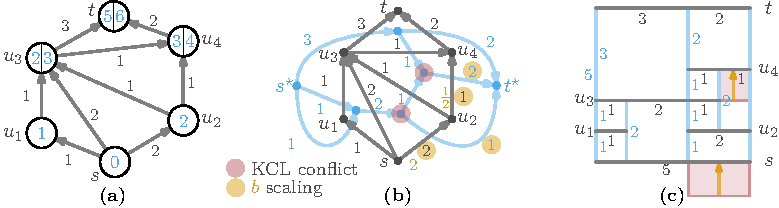
\includegraphics[page=1]{networkAnalyzes/figures/AnalogiesSusceptanceScaling.pdf}
    % 
    \caption[The geometric interpretation of a susceptance scaling.]{We use the
    example graph of~\textcite[p.18]{Fel13} that is also used
    in~\cref{ch:network-analyzes:fig:AnalogiesFlowDualSquares}. The
    \textcolor{SUSCEPTANCE}{susceptances}
    are~$\textcolor{SUSCEPTANCE}{\glssymbol{susceptance}\equiv 1}$ and we
    neglect the \textcolor{CAPACITY}{capacities} meaning~$\textcolor{CAPACITY}{
    \glssymbol{capacity}\equiv\infty}$. We write the flows~\glssymbol{flow} on
    the edges or on the rectangle's side. (a) We apply some feasible
    flow~\textcolor{PRIMALGRAPH}{\glssymbol{flow}} (\ie, complying the~\gls{kcl}
    and capacity constraints only)
    on~\textcolor{PRIMALGRAPH}{graph~\glssymbol{graph}}. The feasible
    flow~\textcolor{PRIMALGRAPH}{\glssymbol{flow}} is not a feasible electrical
    flow, since the voltage angles (distance
    labels))~\textcolor{THETA}{\glssymbol{voltageangle}} at the
    vertices~\tikzVertex are not unique. The latter can be seen in the double
    assignments at~$\vertexa_3,\vertexa_4,\sink\in\glssymbol{vertices}$. Thus,
    the~\gls{kvl} is violated. (b) It is always possible to transform a feasible
    flow~\textcolor{PRIMALGRAPH}{\glssymbol{flow}} into a feasible electrical
    flow~$\textcolor{PRIMALGRAPH}{\glssymbol{flow}'}$ by scaling the
    susceptances~$\textcolor{SUSCEPTANCE}{\glssymbol{susceptance}}$ at certain
    edges such that the
    ratio~$\nicefrac{\textcolor{PRIMALGRAPH}{\glssymbol{flow}}}
    {\textcolor{DUALGRAPH}{\glssymbol{voltageangledifference}}} \equiv
    \nicefrac{\textcolor{PRIMALGRAPH}{\glssymbol{flow}_{\glssymbol{graph}}}}{
    \textcolor{DUALGRAPH}{\glssymbol{flow}_{\glssymbol{dualgraph}}}}
    \equiv \textcolor{SUSCEPTANCE}{\glssymbol{susceptance}}$ changes the flow~$
    \textcolor{DUALGRAPH}{\glssymbol{flow}_{\glssymbol{dualgraph}}}$ in such a
    way that it becomes feasible (\ie, complying~\gls{kcl} and thus, \gls{kvl})
    as long as the \textcolor{SUSCEPTANCE}{susceptance~\glssymbol{susceptance}}
    is not restricted
    meaning~$\textcolor{SUSCEPTANCE}{\glssymbol{susceptance}\in[0,\infty]}$. (c)
    In the geometric setting a \textcolor{SUSCEPTANCE}{susceptance} scaling
    represents an aspect ratio scaling (indicated by the
    \textcolor{SUSCEPTANCE}{arrows $\uparrow$}). The bottom right box would
    exceed the outer rectangle by one unit without the susceptance scaling
    of~$\textcolor{SUSCEPTANCE}{2}$. Without the susceptance scaling of~$
    \textcolor{SUSCEPTANCE}{\nicefrac{1} {2}}$ there would be a gap of one unit
    in the right center.}
    % 
    \label{ch:network-analyzes:fig:AnalogiesSusceptanceScaling}
\end{figure}
% 
%%%%%%%%%%%%%%%%%%%%%%%%%%%%%%%%%%%%%%%%%%%%%%%%%%%%%%%%%%%%%%%%%%%%%%%%%%%%%%%
\section{The Balancing Property}
\label{ch:network-analyzes:sec:balancing-property}
%%%%%%%%%%%%%%%%%%%%%%%%%%%%%%%%%%%%%%%%%%%%%%%%%%%%%%%%%%%%%%%%%%%%%%%%%%%%%%%
% 
Electrical flows have a property of balancing meaning the flows do not congest
certain edges but spread the load over multiple paths from~\source to~\sink.
Note that this is the main difference to graph-theoretical flows that
try---while maximized---to congest all edges as much as possible. The balancing
property of electrical flows is equivalent to flows that minimize the total
losses (\cref{ch:network-analyzes:eq:minimize-losses-quadratic-eq}).
% 
\begin{equation}
    % 
    \min~\sum_{\edge\in\glssymbol{undirectededges}}
    \nicefrac{\glssymbol{flow}(\edge)^2}{\glssymbol{susceptance}(\edge)},
    % 
    \label{ch:network-analyzes:eq:minimize-losses-quadratic-eq}
\end{equation}
% 
which is a quadratic function~\parencite[p.275; Section~2.2, Energy
Equation]{Chr11}. In this section, we describe this property in terms of
simultaneous flows using algorithmic properties that exploit the aforementioned
structure (see~\cref{ch:network-analyzes:obs:quadratic-relationship})

\textcite[p.404; Section~3]{For56} introduced the duality between maximum flows
and shortest paths in which a minimum cut in~\glssymbol{graph} corresponds to a
shortest path in the dual graph~\glssymbol{dualgraph}. To use shortest paths, we
first introduce a distance metric for power grids. The distance between two
vertices is usually the length of an edge or time to pass that edge. The
distance in an electrical network, is given by the potential
difference~$
    % 
    \glssymbol{voltageangle}(\vertexc) 
    -
    \glssymbol{voltageangle}(\vertexa)
    % 
$ that is the voltage angle difference~$
    % 
    \glssymbol{voltageangledifference}(\vertexa,\vertexc)
    % 
$.
 
For a given flow~\glssymbol{flow} the voltage angle difference on
any~\vertexa-\vertexc-path~$\fpath{}{\vertexa}{\vertexc}$ is given
in~\cref{ch:network-analyzes:sec:mathematical-model:eq:actual-voltage-angle-difference}
and is derived
from~\cref{ch:network-analyzes:sec:mathematical-model:eq:kvl-ohm-function-writing}.
We now give a generalization of the voltage angle difference~$
\glssymbol{voltageangledifference}$ that is original defined on edges to the
voltage angle difference on paths that is a distance
function~$\glssymbol{voltageangledifference}\colon\glssymbol{pathset}\to\mathbb{F}$,
where~$
\mathbb{F}$ is a field (\eg, \reals) and~$\glssymbol{pathset}$ is a set of
paths. Note that the equations that are build
from~\cref{ch:network-analyzes:sec:mathematical-model:eq:actual-voltage-angle-difference}
constitute a matrix and the generalization is a simple sum of the rows that
result
in~\cref{ch:network-analyzes:sec:mathematical-model:eq:kvl-ohm-function-writing}.
%
\begin{equation}
    \glssymbol{voltageangledifference}(\fpath{}{\vertexa}{\vertexc})
    \coloneqq
    \sum_{(i,j)\in\fpath{}{\vertexa}{\vertexc}}\frac{\glssymbol{flow}(i,j)}
    {\glssymbol{susceptance}(i,j)},
    % 
    \label{ch:network-analyzes:sec:mathematical-model:eq:actual-voltage-angle-difference}
\end{equation}
% 
for a path~$\fpath{}{\vertexa}{\vertexc}\in\glssymbol{pathset}$
with~$\vertexa,\vertexc\in\glssymbol{vertices}$. 
% 
For electrical flows the metric is~$\nicefrac{\glssymbol{flow}(\edge)}{
\glssymbol{susceptance}(\edge)}$ deduced from~\cref{ch:network-analyzes:sec:mathematical-model:eq:actual-voltage-angle-difference}.
% 
The~\acrlong{sppp} (\gls{sppp}) computes a path with minimum length~$
\fpath{\gls{spp}}{\source}{\sink}\coloneqq$
$\min_{\fpath{}{\source}{\sink}\in\glssymbol{pathset}} $
$\sum_{\edge\in\fpath{}{\source}{\sink}}$
$\nicefrac{\glssymbol{flow}(\edge)}{\glssymbol{susceptance}(\edge)}
$. Contrary, the~\acrlong{lppp} (\gls{lppp}) computes a
path that has the longest distance between two vertex pairs~$
\fpath{\gls{lpp}}{\source}{\sink}\coloneqq $
$\max_{\fpath{}{\source}{\sink}\in\glssymbol{pathset}}$
$\sum_{\edge\in\fpath{}{\source}{\sink}}$
$\nicefrac{\glssymbol{flow}(\edge)}{\glssymbol{susceptance}(\edge)}$.  

From the previous section (see
especially~\cref{ch:network-analyzes:sec:mathematical-model:eq:kvl-matrix-writing,ch:network-analyzes:sec:mathematical-model:eq:kvl-ohm-function-writing})
we know that the voltage angle assignments are unique and thus, we get the
following observation that is illustrated
in~\cref{ch:network-analyzes:fig:LongestVsShortestPathAnalogies}.

The distance between to vertices~$\vertexa,\vertexc\in\glssymbol{vertices}$
with~$(\vertexa,\vertexc)\in\glssymbol{edges}$ is given by the voltage angle
difference~$
% 
\glssymbol{voltageangledifference}(\vertexa,\vertexc) 
\coloneqq
\glssymbol{voltageangle}(\vertexc) - \glssymbol{voltageangle}(\vertexa)
% 
$ with voltage angles~\glssymbol{voltageangle} that can be interpreted as 
distance labels. The voltage angle difference (\ie, the electrical distance)
for a path~$\glssymbol{path}(\source,\sink)$ is given by~$
\glssymbol{voltageangledifference}(\glssymbol{path}(\source,\sink))
\!=\!
\sum_{(\vertexa,\vertexc)\in\glssymbol{path} (\source,\sink)}\! 
\glssymbol{voltageangledifference}(\vertexa,\vertexc) 
\!=\!
\sum_{(\vertexa,\vertexc)\in\glssymbol{path}(\source,\sink)}\! 
\nicefrac{\glssymbol{flow}(\vertexa,\vertexc)}{
\glssymbol{susceptance}(\vertexa,\vertexc)}
$.
% 
\begin{lemma}[Balancing Flow Property]
    Given a primal graph~\glssymbol{graph} and its dual
    graph~\glssymbol{dualgraph}, for which the shortest path~$
    % 
        \fpath{
            \gls{spp}
        }{\source}{\sink}
        \in
        \glssymbol{pathset}(\glssymbol{graph})
    % 
    $ in~\glssymbol{graph} (respectively longest path~$
        % 
        \fpath{
            \gls{lpp}
        }{\source}{\sink}
        \in
        \glssymbol{pathset}(\glssymbol{graph})
        % 
    $) can differ to the shortest path~$
    % 
        \fpath{
            \gls{spp}
        }{\source}{\sink}
        \in
        \glssymbol{pathset}(\glssymbol{dualgraph})
    % 
    $ 
    in~\glssymbol{dualgraph} (respectively longest path~$
        % 
        \fpath{
            \gls{lpp}
        }{\source}{\sink}
        \in
        \glssymbol{pathset}(\glssymbol{dualgraph})
        % 
    $). A flow~\glssymbol{flow} is an electrical flow if and only if the longest
    and shortest path have the same length~$
    % 
        \glssymbol{voltageangledifference}(\fpath{\gls{spp}}{\source}{\sink})
        = 
        \glssymbol{voltageangledifference}(\fpath{\gls{lpp}}{\source}{\sink})
    % 
    $ in~$\glssymbol{graph}$
    with~$\source,\sink\in\glssymbol{vertices}(\glssymbol{graph})$ and~$
    % 
        \glssymbol{voltageangledifference}(
            \fpath{\gls{spp}}{\source^\star}{\sink^\star}
        )
        = 
        \glssymbol{voltageangledifference}(
            \fpath{\gls{lpp}}{\source^\star}{\sink^\star}
        )
    % 
    $ in~$\glssymbol{dualgraph}$
    with~$\source^\star,\sink^\star\in\glssymbol{vertices}(\glssymbol{dualgraph})$
    (\wrt~the distance
    metric~$\nicefrac{\glssymbol{flow}}{\glssymbol{susceptance}}$).
    % 
    \label{ch:network-analyzes:lem:balancing-flow-property}
\end{lemma}
% 
\begin{proof}
    $\Rightarrow\colon$ 
    % 
    First we show the one direction, where~\glssymbol{flow} is a feasible
    electrical flow, which implies that the length of all paths is equivalent~$
        \glssymbol{voltageangledifference}(\fpath{\gls{spp}}{\source}{\sink})
        =
        \glssymbol{voltageangledifference}(\fpath{\gls{lpp}}{\source}{\sink})
    $.

    Let~\glssymbol{flow} be a feasible electrical flow. 
    If~$
        % 
        \glssymbol{voltageangledifference}(\fpath{\gls{spp}}{\source}{\sink}) 
        \neq
        \glssymbol{voltageangledifference}(\fpath{\gls{lpp}}{\source}{\sink}) 
        % 
    $ in~\glssymbol{graph} with~$
    \source,
    \sink
    \in
    \glssymbol{vertices}(\glssymbol{graph})
    % 
    $ then there is no unique voltage angle
    assignment~$\glssymbol{voltageangle}(\vertexa)$ for all~$\vertexa\in
    \glssymbol{vertices}(\glssymbol{graph})$. This implies that~\glssymbol{flow}
    does not comply with the~\gls{kvl}
    (see~\cref{ch:network-analyzes:sec:mathematical-model:eq:kvl-ohm-function-writing}).
    If~$
        % 
        \glssymbol{voltageangledifference}(\fpath{\gls{spp}}{\source^\star}
        {\sink^\star})
        \neq
        \glssymbol{voltageangledifference}(\fpath{\gls{lpp}}{\source^\star}{\sink^\star})
        % 
    $ in~\glssymbol{dualgraph} with~$
    \source^\star,
    \sink^\star
    \in
    \glssymbol{vertices}(\glssymbol{dualgraph})
    % 
    $ then there is no unique voltage angle assignment in~\glssymbol{dualgraph} 
    (see~\cref{ch:network-analyzes:thm:electrical-flow-based-definition}), 
    % 
    which means that~\glssymbol{flow} does not comply with the~\gls{kcl}
    (see~\crefrange{ch:network-analyzes:sec:mathematical-model:eq:kcl-matrix-writing:1}{ch:network-analyzes:sec:mathematical-model:eq:kcl-matrix-writing:3}).
    Any one of the two cases would be a contradiction to~\glssymbol{flow} being
    a feasible electrical flow
    (see~\cref{ch:network-analyzes:sec:mathematical-model:def:kvl-kcl-feasible-flow}).

    $\Leftarrow\colon$
    With the other direction, we show that if~$
        % 
        \glssymbol{voltageangledifference}(\fpath{\gls{spp}}{\source}{\sink})
        =
        \glssymbol{voltageangledifference}(\fpath{\gls{lpp}}{\source}{\sink})
        % 
    $ then this implies that~\glssymbol{flow} is a feasible electrical flow.
    % 
    Given two paths from~\source to~\sink denoted by~$
        % 
        \fpath{1}{\source}{\sink},
        \fpath{2}{\source}{\sink}
        \in
        \glssymbol{pathset}
        % 
    $ that merge at vertex~$x$, meaning~$
        % 
        \fpath{1}{x}{\sink} 
        = 
        \fpath{2}{x}{\sink} 
        \eqqcolon 
        \glssymbol{path}
        % 
    $. In addition, we have given the distance metric~$
        % 
        \nicefrac{
            \glssymbol{flow}(\vertexa,\vertexc)
        }{
            \glssymbol{susceptance}(\vertexa,\vertexc)
        }
        % 
    $ then from~$
    % 
        \glssymbol{voltageangledifference}\big(\fpath{1}{\source}{\sink}\big)
        =
        \glssymbol{voltageangledifference}\big(\fpath{2}{\source}{\sink}\big)
    % 
    $ using the distance metric follows 
    % 
    \begin{align*}
        % 
        \sum_{(\vertexa,\vertexc)\in\fpath{1}{\source}{\sink}}
        \frac{
            \glssymbol{flow}(\vertexa,\vertexc)
        }{
            \glssymbol{susceptance}(\vertexa,\vertexc)
        }
        &=
        \sum_{(\vertexa,\vertexc)\in\fpath{2}{\source}{\sink}}
        \frac{
            \glssymbol{flow}(\vertexa,\vertexc)
        }{
            \glssymbol{susceptance}(\vertexa,\vertexc)
        }.
    \end{align*}
    % 
    We define the voltage angles on the source~\source and sink~\sink to
    be~$\glssymbol{voltageangle} (\source)\coloneqq 0$, and~$
    % 
        \glssymbol{voltageangle}(\sink)
        \coloneqq 
        \glssymbol{voltageangledifference}
        \big(
            \fpath{1}{\source}{\sink}
        \big)
        =
        \glssymbol{voltageangledifference}
        \big(
            \fpath{2}{\source}{\sink}
        \big)
    % 
    $. 

    \begin{align*}
        \glssymbol{voltageangle}(\source) 
        + 
        \sum_{ (\vertexa,\vertexc) \in \fpath{1}{\source}{x} }
        \frac{
            \glssymbol{flow}(\vertexa,\vertexc)
        }{
            \glssymbol{susceptance}(\vertexa,\vertexc)
        }
        +
        \glssymbol{path}
        =
        \glssymbol{voltageangle}(\sink)
        \\
        \glssymbol{voltageangle}(\source) 
        + 
        \sum_{ (\vertexa,\vertexc) \in \fpath{2}{\source}{x} }
        \frac{
            \glssymbol{flow}(\vertexa,\vertexc)
        }{
            \glssymbol{susceptance}(\vertexa,\vertexc)
        }
        +
        \glssymbol{path}
        =
        \glssymbol{voltageangle}(\sink)
    \end{align*}

    Since~$\glssymbol{path} = \fpath{1}{x}{\sink} = \fpath{2}{x}{\sink}$,
    $\glssymbol{voltageangle} (\source) = 0$, and the voltage angle~$
    % 
        \glssymbol{voltageangle}(\sink) 
        = 
        \glssymbol{voltageangledifference}
        \big(
            \fpath{1}{\source}{\sink}
        \big)
        = 
        \glssymbol{voltageangledifference}
        \big(
            \fpath{2}{\source}{\sink}
        \big)
    % 
    $. It follows that 
    \begin{align*}
        % 
        \sum_{(\vertexa,\vertexc)\in\fpath{1}{\source}{x}}
        \frac{
            \glssymbol{flow}(\vertexa,\vertexc)
        }{
            \glssymbol{susceptance}(\vertexa,\vertexc)
        }
        &=
        \sum_{(\vertexa,\vertexc)\in\fpath{2}{\source}{x}}
        \frac{
            \glssymbol{flow}(\vertexa,\vertexc)
        }{
            \glssymbol{susceptance}(\vertexa,\vertexc)
        }
        &=
        \glssymbol{voltageangle}(\sink) 
        -
        \glssymbol{voltageangle}(\source)
        -
        \glssymbol{path} 
        .
    \end{align*}
    % 
    Thus, the distances from the source~\source to the vertex~$x$ are the same
    meaning~$
    % 
        \glssymbol{voltageangledifference}\big(\fpath{1}{\source}{x}\big)
        $
        $
        =
        \glssymbol{voltageangledifference}\big(\fpath{2}{\source}{x}\big)
        \eqqcolon 
        \glssymbol{voltageangle}(x)
    % 
    $.
    % 
    We can recursively proceed, which gives us the following equality. 
    % 
    \begin{align*}
        % 
        \sum_{(\vertexa,\vertexc)\in\fpath{1}{\source}{x}}
        \glssymbol{voltageangledifference}(\vertexa,\vertexc)
        &=
        \sum_{(\vertexa,\vertexc)\in\fpath{2}{\source}{x}}
        \glssymbol{voltageangledifference}(\vertexa,\vertexc)
        % 
    \end{align*}
    % 
    This relationship is known
    from~\cref{ch:network-analyzes:sec:mathematical-model:eq:kvl-ohm-function-writing} 
    and restated by~$
    % 
        \glssymbol{voltageangledifference}(\vertexa,\vertexc)
        \coloneqq
        \big(
            \glssymbol{voltageangle}(\vertexc) 
            - 
            \glssymbol{voltageangle}(\vertexa)
        \big) 
        = \frac{
            \glssymbol{flow}(\vertexa,\vertexc)
        }{
            \glssymbol{susceptance}(\vertexa,\vertexc)
        }
    % 
    $.
    % 
    The phase angles on each side cancel each other out, but the source~\source
    and the sink~\sink.
    % 
    \begin{align*}
        \begin{aligned}
            \big(
                \glssymbol{voltageangle}(\vertexa_1) 
                - \glssymbol{voltageangle}(\source)
            \big)
            &+
            \big(
                \glssymbol{voltageangle}(\vertexa_2) 
                - 
                \glssymbol{voltageangle}(\vertexa_1)
            \big)
            &+&
            \big(
                \glssymbol{voltageangle}(\vertexa_3) 
                - 
                \glssymbol{voltageangle}(\vertexa_2)
            \big)
            +
            \dots
            \\
            % +
            \dots
            &+
            \big(
                \glssymbol{voltageangle}(\vertexa_n) 
                - 
                \glssymbol{voltageangle}(\vertexa_{n-1})
            \big)
            &+&
            \big(
                \glssymbol{voltageangle}(\vertexa_{\sink}) 
                - 
                \glssymbol{voltageangle}(\vertexa_n)
            \big)
            =
            \big(
                \glssymbol{voltageangle}({\sink}) 
                - 
                \glssymbol{voltageangle}({\source})
            \big)
        \end{aligned}
    \end{align*}
    % 
    Since the source~\source and the sink~\sink are for both
    paths~$\fpath{1}{\source}{\sink},\fpath{2}{\source}
    {\sink}\in\glssymbol{pathset}$ the same and both paths have the same
    distance~$
    % 
        \glssymbol{voltageangledifference}\big(\fpath{1}{\source}{\sink}\big)
        =
        \glssymbol{voltageangledifference}\big(\fpath{2}{\source}{\sink}\big)
    % 
    $ the voltage angle assignments are unique. We get
    $
    % \glssymbol{flow}(\source,\sink)
    % =
    % \glssymbol{susceptance}(\source,\sink)
    \big(
        \glssymbol{voltageangle}(\sink) 
        - 
        \glssymbol{voltageangle}(\source)
    \big) 
    =
    \sum_{(\vertexa,\vertexc)\in\fpath{1}{\source}{\sink}}
    \frac{
        \glssymbol{flow}(\vertexa,\vertexc)
    }{
        \glssymbol{susceptance}(\vertexa,\vertexc)
    }
    =
    \sum_{(\vertexa,\vertexc)\in\fpath{2}{\source}{\sink}}
    \frac{
        \glssymbol{flow}(\vertexa,\vertexc)
    }{
        \glssymbol{susceptance}(\vertexa,\vertexc)
    }
    = \frac{
        \glssymbol{flow}(\source,\sink)
    }{
        \glssymbol{susceptance}(\source,\sink)
    }.
    $

    % % 
    % From~\cref{ch:network-analyzes:sec:mathematical-model:eq:kvl-ohm-function-writing}
    % we know that~$
    % \glssymbol{voltageangledifference}(\vertexa,\vertexc)
    % \coloneqq
    % \big(
    %     \glssymbol{voltageangle}(\vertexc) 
    %     - 
    %     \glssymbol{voltageangle}(\vertexa)
    % \big) 
    % = \frac{
    %     \glssymbol{flow}(\vertexa,\vertexc)
    % }{
    %     \glssymbol{susceptance}(\vertexa,\vertexc)
    % }$. 
\end{proof}

\begin{figure}[t!]
    % 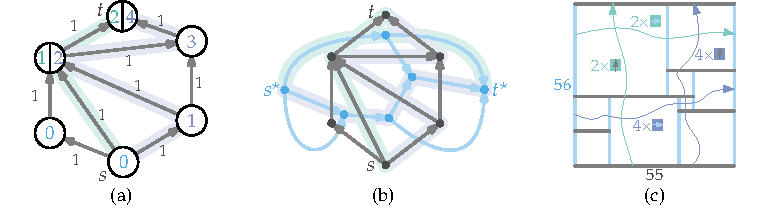
\includegraphics[page=1]{networkAnalyzes/figures/LongestVsShortestPathAnalogies.pdf}
    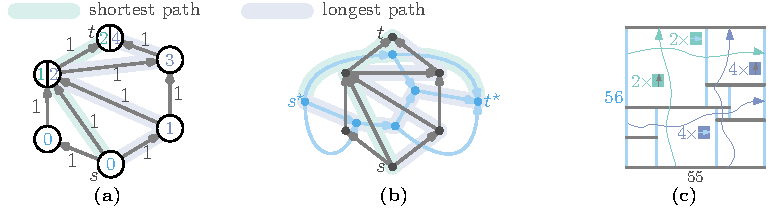
\includegraphics[page=1]{networkAnalyzes/figures/Property-of-Balancing.pdf}
    % 
    \caption[The property of balancing.]{We use the example graph
    of~\textcite[p.18]{Fel13}. The~\textcolor{SUSCEPTANCE}{susceptances
    are~$\glssymbol{susceptance}\equiv 1$} and we neglect the capacities
    meaning~\textcolor{CAPACITY}{$\glssymbol{capacity}\equiv\infty$}. (a)
    Assuming unit distances the \textcolor{KITgreen70}{shortest
    path~$\fpath{\gls{spp}}{\source}{\sink}$} and \textcolor{KITblue70}{longest
    path~$\fpath{\gls{lpp}}{\source}{\sink}$} in the original graph with the
    corresponding distance labels at the vertices have length
    \textcolor{KITgreen70}{2} and \textcolor{KITblue70}{4}, respectively. (b)
    The \textcolor{KITgreen70}{shortest} and \textcolor{KITblue70}{longest} path
    in the~\textcolor{PRIMALGRAPH}{primal graph~\glssymbol{graph}}
    and~\textcolor{DUALGRAPH}{dual graph~\glssymbol{dualgraph}} have the same
    length. However, adding an edge from~\source to~\sink describes that this is
    not always the case. (c) The \textcolor{KITgreen70}{shortest path~$
    \fpath{\gls{spp}}{\source}{\sink}$} and
    \textcolor{KITblue70}{longest path~$\fpath{\gls{lp}}{\source}{\sink}$}
    describe the \textcolor{KITgreen70}{minimum} and \textcolor{KITblue70}
    {maximum} number of rectangles (here squares) that are stacked in either
    directions.}
    % 
    \label{ch:network-analyzes:fig:LongestVsShortestPathAnalogies}
\end{figure}
% 
The intuition that electricity follows the path of the least resistance and
tries to balance itself leads us to a~\emph{balanced flow}, where all paths have
the same length from any vertex to any other vertex. First, we introduce
shortest paths for power grids that represent one part of the intuition namely
the path with the least resistance. Note that vertex label differences always
sum up to zero and thus, these labels, too. Recall that this is exactly the same
behavior as
in~\cref{ch:network-analyzes:sec:mathematical-model:eq:kvl-ohm-function-writing}
for the voltage angles.
% 
A vertex~\vertex that
violates~\crefrange{ch:network-analyzes:sec:mathematical-model:eq:kcl-matrix-writing:1}{ch:network-analyzes:sec:mathematical-model:eq:kcl-matrix-writing:3}
has an excess~$\glssymbol{netflow}(\vertex)\not= 0$. The excess represents the
amount of flow that has to be reduced or increased in~\vertex's incoming or
outgoing flow, respectively. From the duality of the~\acrlong{mfp}
and~\acrlong{sppp}~\parencite[p.404; Section~3]{For56} and the aforementioned
discussion on the duality of the~\gls{kcl} and~\gls{kvl} constraints, we get the
following observation.
%
\begin{observation}
A feasible~\gls{kvl} flow can be computed by a shortest path in the primal
graph~\glssymbol{graph}.
% 
\label{ch:network-analyzes:sec:mathematical-model:lem:KVL-voltage-angles}
\end{observation}
% 
Note that a feasible~\gls{kvl} flow is not restricted to shortest paths as long
as the voltage angle assignment is unique. Contrary a feasible~\gls{kcl} flow
can be computed by a shortest path in the dual graph~\glssymbol{dualgraph}. This
provides us a deeper understanding of why shortest paths work in some cases
quite well~\parencite{Gra18}.
% 
In addition, the maximum flow values of the primal
graph~$\glssymbol{flowvalue}(\glssymbol{graph})$ and dual
graph~$\glssymbol{flowvalue}(\glssymbol{dualgraph})$ represent upper bounds for
the maximum feasible electrical flow.
% 
\begin{lemma}%
    A~\acrlong{mf} (\gls{mf}) in graph~\glssymbol{graph} and its dual
    graph~\glssymbol{dualgraph} represent two upper bounds for
    the~\acrlong{mpfp} (\gls{mpfp}).
\end{lemma}%
% 
However, the electrical flow does not always reach a~\gls{mf}. We discuss this
in more detail in~\cref{ch:switching,ch:facts}. 
% 
We use the balancing property in the next section to tackle~\gls{kcl} conflicts.
% 
%%%%%%%%%%%%%%%%%%%%%%%%%%%%%%%%%%%%%%%%%%%%%%%%%%%%%%%%%%%%%%%%%%%%%%%%%%%%%%%
\section{An Algorithm for Electrical Flows on s-t Planar Graphs}
\label{ch:network-analyzes:sec:algorithm}
%%%%%%%%%%%%%%%%%%%%%%%%%%%%%%%%%%%%%%%%%%%%%%%%%%%%%%%%%%%%%%%%%%%%%%%%%%%%%%%
% 
In this section, we discuss an algorithm for s-t planar graphs
for~\gls{dc}~\gls{feas} and~\gls{mpfp}. For the algorithm, we mainly use the
duality concepts of the aforementioned sections and the reformulation
of~\gls{dc}~\gls{feas} using simultaneous flow on~\glssymbol{graph}
and~\glssymbol{dualgraph}
(\cref{ch:network-analyzes:simultaneous-flow-representation}).

The basic idea of the algorithm is that we switch between the primal
graph~\glssymbol{graph} and the dual graph~\glssymbol{dualgraph} and fix each
time the~\gls{kcl} property of the flow that might lead to~\gls{kcl} conflict in
its dual graph. The property of balancing
(see~\cref{ch:network-analyzes:sec:balancing-property}) is used to describe how
we fix~\gls{kcl} conflicts and that the algorithm terminates. 
% The integrality of
% an electrical flow is then used to show that the algorithm terminates.
In~\cref{ch:network-analyzes:algo:s-t-power-flow-algorithm}, we show the
algorithm to compute an electrical flow in an~\source-\sink biconnected planar
graph. In the following, we will describe each part of the algorithm in more
detail.
% 
%%%%%%%%%%%%%%%%%%%%%%%%%%%%%%%%%% ALGORITHM %%%%%%%%%%%%%%%%%%%%%%%%%%%%%%%%%%%
%
\wormhole{bit:ch:switching:sec:exploit_structural_characteristics:subsec:dtp:alg:shortest_theta_path}
\def\HiLi{\leavevmode\rlap{\hbox to \hsize{\color{HiLi}\leaders\hrule
height .9\baselineskip depth 1.3ex\hfill}}}
\begin{algorithm}[tb!]%
\SetAlgoLined
%%%%%%%%%%%%%%%%%%%%%%%%%%%%%%%%%%
% 
\KwData{A network~\dcnetworktuple with~$\fmagnitude{\glssymbol{generators}} = 1$ (\ie,
$\{\source\} = \glssymbol{generators}$), $\fmagnitude{\glssymbol{consumers}} = 1$ 
(\ie, $\{\sink\} = \glssymbol{consumers}$), $\underline{\glssymbol{capacity}}\equiv 0$, and~$
\overline{\glssymbol{capacity}}\equiv\infty$.}
% 
\KwResult{Flow~$\glssymbol{flow}(\vertexa,\vertexc)$ for all $
(\vertexa,\vertexc)\in\glssymbol{edges}$, flow value~$\glssymbol{flowvalue}(\glssymbol{flow},\glssymbol{network})$, and
voltage angles~$\glssymbol{voltageangle} (\vertexa)$
with~$\vertexa\in\glssymbol{vertices}$.}
% 
% INITIALIZATION %%%%%%%%%%%%%%%%%%%%%%%%%%%%%%%%%%%%%%%%%%%%%%%%%%%%%%%%%%%%
$\glssymbol{graph} =
\algoBipolarSubgraphOf(\glssymbol{graph},\source,\sink)$\hspace*{-1mm}%
\label{ch:network-analyzes:algo:stpf:bipolarSubgraph}
\Comment*{\color{KITblack30} see~\cref{ch:network-analyzes:sec:bipolar-orientation}}%
% 
$\embedding = \algoplanarembedding(\glssymbol{graph})$\hspace*{-1mm}%
\label{ch:network-analyzes:algo:stpf:planarEmbedding}
\Comment*{\color{KITblack30} PQ-Tree; see~\cref{ch:network-analyzes:sec:planar-embedding-dual-graph-construction}}%
% 
$\big(
    \glssymbol{dualgraph}, 
    \glssymbol{susceptance}^\star, 
    \oneToOneMap
        \colon
        \glssymbol{edges}(\glssymbol{graph})
        \to
        \glssymbol{edges}(\glssymbol{dualgraph})
\big) 
= 
\algoconstructDualGraphOf(
    \glssymbol{graph}(\embedding),
    \glssymbol{susceptance}
)$\hspace*{-1mm}%
\label{ch:network-analyzes:algo:stpf:constructDualGraph:1}
% \Comment*{\color{KITblack30} Bijective fct.~\oneToOneMap}%
\Comment*{\color{KITblack30}\cref{ch:network-analyzes:sec:planar-embedding-dual-graph-construction}}
% 
\Comment{\color{KITblack30} Augment flow along an incident edge at
 source~\source}%
$\glssymbol{flow}\equiv 0$;~$\glssymbol{flow}(\source,\vertexa) = 1$ for
some edge~$(\source,\vertexa)\in\glssymbol{edges}
(\glssymbol{graph})$\;
\label{ch:network-analyzes:algo:stpf:initialFlow}
% 
$(\subgraph, \glssymbol{susceptance}, \source, \sink) = (\glssymbol{graph},
\glssymbol{susceptance}, \source, \sink)$\;
\label{ch:network-analyzes:algo:stpf:GraphRenaming}
% 
$\excessSet = \{\vertexa\in\glssymbol{vertices}(\subgraph)\mid\glssymbol{netflow}(\vertexa)\not=0\}$\;
\label{ch:network-analyzes:algo:stpf:set-of-vertices-with-excess:1}
% 
% LOOP UNTIL QUEUE IS EMPTY %%%%%%%%%%%%%%%%%%%%%%%%%%%%%%%%%%%%%%%%%%%%%%%%%
\While(\Comment*[f]{\color{KITblack30}Check~\gls{kcl} property in \subgraph})
{$\excessSet\not=\emptyset$}
{ % while
    $\glssymbol{flow}_{\subgraph}$ = \resolveConflict{\subgraph, \excessSet,
    \glssymbol{susceptance}, \source, \sink, $\glssymbol{flow}_{\subgraph}$
    }\hspace*{-1mm}%
    \label{ch:network-analyzes:algo:stpf:ResolveKclConflict}\;
    % \Comment*{\color{KITblack30}
    % see~\cref{ch:network-analyzes:algo:resolve-kcl-Conflict}
    % }%
    % 
    $(\subgraph^\star, \glssymbol{susceptance}^\star, \source^\star,
    \sink^\star) = (\subgraph, \glssymbol{susceptance}, \source, \sink)$;
    % 
    $(\subgraph, \glssymbol{susceptance}, \source, \sink) 
    = 
    \algoDualGraphOf(\subgraph^\star, \glssymbol{susceptance}^\star,
    \source^\star, \sink^\star)$\;
    % 
    \label{ch:network-analyzes:algo:stpf:constructDualGraph:2}
    % 
    $\glssymbol{flow}_\subgraph(\edge) = \glssymbol{flow}_{\subgraph^\star}(\oneToOneMap(\edge))\cdot\glssymbol{susceptance}
    (\edge)$\;
    \label{ch:network-analyzes:algo:stpf:flowOneToOneMapping:2}
 %    \Comment{\color{KITblack30} Invariant squares with same aspect ratio, \ie,
 % flow on the edge and dual edge have the same value }%
    % 
    $\excessSet = \{\vertexa\in\glssymbol{vertices}(\subgraph)\mid
    \glssymbol{netflow}
    (\vertexa)\not=0\}$\hspace*{-1mm}%
    \label{ch:network-analyzes:algo:stpf:set-of-vertices-with-excess:2}
    \Comment*{\color{KITblack30} New~\gls{kcl} conflicts in the dual graph}%
}
%%%%%%%%%%%%%%%%%%%%%%%%%%%%%%%%%%
% \caption{\source-\sink-\PFu~(\gls{pf}) Algorithm}%
\caption{\source-\sink Planar~\gls{dc}~\gls{feas}(\glssymbol{network})
 \&~\source-\sink Planar~\gls{mpfp}(\glssymbol{network})}
\label{ch:network-analyzes:algo:s-t-power-flow-algorithm}% 
\end{algorithm}% 
% 
%%%%%%%%%%%%%%%%%%%%%%%%%%%%%%%%%%%%%%%%%%%%%%%%%%%%%%%%%%%%%%%%%%%%%%%%%%%%%%%
\subsection{Bipolar Orientation}
\label{ch:network-analyzes:sec:bipolar-orientation}
%%%%%%%%%%%%%%%%%%%%%%%%%%%%%%%%%%%%%%%%%%%%%%%%%%%%%%%%%%%%%%%%%%%%%%%%%%%%%%%
% 
In this section, we focus on the function~$\algoBipolarSubgraphOf(
\glssymbol{graph},\source,\sink)$
in~\cref{ch:network-analyzes:algo:stpf:bipolarSubgraph}
of~\cref{ch:network-analyzes:algo:s-t-power-flow-algorithm}. 
% 
Each simultaneous flow has a specific direction, which is naturally given by an
electrical flow that is in general a~\acrlong{dag} (\gls{dag}). Another
interpretation can be given from the rectangular representation that has
a~\gls{dag} as a visibility graph~\parencite[pp.12f.]{Fel13}. The latter means
that there is an edge between two vertices if there is a segment between them.
See for
example~\cref{ch:network-analyzes:fig:AnalogiesFlowDualSquares}\screen{c},
where the horizontal segments~$\vertexa_3$ and~$\sink$ are visible to each
other, since there is a vertical segment that connects both segments directly.
The visibility graph is given
in~\cref{ch:network-analyzes:fig:AnalogiesFlowDualSquares}\screen{b}, where we
represent the visibility of~$\vertexa_3$ and~\sink by an edge~$
(\vertexa_3,\sink)$. So if we define a visibility direction, \eg, from bottom to
top (horizontal segment visibility) and from left to right (vertical segment
visibility), we get two directed acyclic visibility graphs as shown
in~\cref{ch:network-analyzes:fig:AnalogiesFlowDualSquares}\screen{b}. Note that
the \acrlong{dag}s (\gls{dag}s) are either called bipolar
orientation~\parencite{Fra95} or~\source-\sink-numbering~\parencite{Eve76}. Such
a numbering gives each vertex~$\vertexa\in\glssymbol{vertices}$ a number within
the range of~$[\source=1,\dots,\fmagnitude{\glssymbol{vertices}}=\sink]$, which
represents a topological order of the vertices.
%
\begin{observation}[Bipolar Duals~{{\parencite[p.13]{Fel13}}}]
    A bipolar orientation in the primal graph~\glssymbol{graph} implies a
    bipolar orientation in the dual graph~\glssymbol{dualgraph}.
\end{observation}
% 
To see the latter, observation let us assume a directed edge~$
(\vertexa_1,\vertexa_2)\in\glssymbol{edges}(\glssymbol{graph})$. This edge is incident to two
faces~$\cycle_1,\cycle_2\in\glssymbol{vertices}(\glssymbol{dualgraph})$. Looking in the direction of
the edge~$(\vertexa_1,\vertexa_2)$, meaning that we look from~$\vertexa_1$
to~$\vertexa_2$ then the face~$\cycle_1$ is to the left of that edge
and~$\cycle_2$ is to the right of that edge. Since we have a bijection of the
edges there is an edge~$
\{\cycle_1,\cycle_2\}\in\glssymbol{undirectededges}(\glssymbol{dualgraph})$. We
define that a direction from~$\vertexa_1$ to~$\vertexa_2$ implies a direction
from~$\cycle_1$ to~$\cycle_2$ and thus, a direction from left to right. Thus, if
there is a bipolar orientation for graph~\glssymbol{graph} this implies a
bipolar orientation for its dual graph~\glssymbol{dualgraph} by definition. An
illustration is given
in~\cref{ch:network-analyzes:fig:AnalogiesFlowDualSquares,ch:network-analyzes:fig:AnalogiesSusceptanceScaling}
b.
% 
\begin{observation}[Biconnectivity Assumption~{{\parencite[p.13]{Fel13}}}]
    If graph~\glssymbol{graph} has a bipolar orientation then it is biconnected.
\end{observation}
% 
Calculating a bipolar orientation takes~$\bigO(\fmagnitude{
\glssymbol{vertices}})$ time~\parencite{Fel13}. An overview of the graph classes
that fulfill the latter property are given by~\textcite[p.212; Theorem 6.19]
{Bat98}. The most interesting classes to us are planar \source-\sink-graphs,
series-parallel digraphs, and planar bipartite digraphs.
% 
%%%%%%%%%%%%%%%%%%%%%%%%%%%%%%%%%%%%%%%%%%%%%%%%%%%%%%%%%%%%%%%%%%%%%%%%%%%%%%%
\subsection{Planar Embedding and Dual Graph Construction}
\label{ch:network-analyzes:sec:planar-embedding-dual-graph-construction}
%%%%%%%%%%%%%%%%%%%%%%%%%%%%%%%%%%%%%%%%%%%%%%%%%%%%%%%%%%%%%%%%%%%%%%%%%%%%%%%
%
Recall that we assume that graph~\glssymbol{graph} is planar. To compute a
planar embedding~\glssymbol{embedding}, we use
in~$\algoplanarembedding(\glssymbol{graph})$
(\cref{ch:network-analyzes:algo:s-t-power-flow-algorithm}
in~\cref{ch:network-analyzes:algo:stpf:planarEmbedding}) a linear-time planarity
testing algorithm~\parencite{Hop74}\parencite[p.345]{Ros86}. These algorithms
construct circular lists in~$\bigO(\fmagnitude{\glssymbol{vertices}})$ that
represent for each vertex an ordered list of its incident edges in clock-wise
order. The latter represents a set of rotations, which we will use to construct
the dual graph~\glssymbol{dualgraph}. This can be done by selecting any edge~$
\{\vertexa,\vertexc\}\in\glssymbol{undirectededges}$ and traverse it in one
direction such as from~$\vertexa$ to~$\vertexc$. Then select the next edge
clockwise at~$\vertexc\in\glssymbol{vertices}$. We proceed this method until we
reach~$\vertexa$. The walk represents a traversal of a face, where~$
(\vertexa,\vertexc)$ represents one boundary edge. We traverse the edge in the
other direction meaning~$(\vertexc,\vertexa)$ that gives us the boundary edges
of the other face that is incident to
edge~$\{\vertexa,\vertexc\}\in\glssymbol{undirectededges}$. We proceed with an
edge that was not traversed in both direction and apply the aforementioned
method. This extracts for each edge the left face~$\cycle_{\leftish}$ and right
face~$\cycle_{\rightish}$ with~$
    % 
    \cycle_{\leftish},
    \cycle_{\rightish}
    \in
    \glssymbol{vertices}(\glssymbol{dualgraph})
    % 
$ and within that, we construct implicitly the edge~$
    % 
    \{
    \cycle_{\leftish}, 
    \cycle_{\rightish}
    \}
    \in
    \glssymbol{undirectededges}(\glssymbol{dualgraph})
    % 
$. The dual graph~\glssymbol{dualgraph} of a graph~\glssymbol{graph} can be
constructed in~$\bigO(\fmagnitude{\glssymbol{vertices}})$.

Since we use the same construction as~\textcite[pp.344ff.; Section~2]{Ros86}, we
assume that the graph is biconnected for the aforementioned construction.
Otherwise, we add---similar to~\textcite[p.345]{Ros86}---dummy edges such
that~\glssymbol{graph} stays planar and becomes biconnected, which is possible
in~$\bigO(\fmagnitude{\glssymbol{vertices}})$. After the construction of the
layout, we will remove the dummy edges, otherwise we would get an electrical
flow for another graph than the input graph.
% 
In addition, to simplify the translation from one graph into the other one, we
define the susceptance~$\glssymbol{susceptance}(\edge)$
for~$\edge\in\glssymbol{undirectededges}(\glssymbol{graph})$ for the dual
graph~$\glssymbol{dualgraph}$ by~$
    % 
    \glssymbol{susceptance}^\star(\oneToOneMap(\edge))
    \coloneqq
    \nicefrac{1}{\glssymbol{susceptance}(\edge)}
    % 
$. This is necessary
for~\cref{ch:network-analyzes:algo:stpf:flowOneToOneMapping:2}
in~\cref{ch:network-analyzes:algo:s-t-power-flow-algorithm}.
%
% \begin{algorithm}[tb!]%
% \SetAlgoLined
% %%%%%%%%%%%%%%%%%%%%%%%%%%%%%%%%%%
% % 
% \KwData{A directed \source-\sink-graph~$\subgraph$,
% $\excessSet\subseteq\glssymbol{vertices}$
% with~$\glssymbol{netflow}(\vertexa)\neq 0$ for all~$\vertexa\in\excessSet$, one
% source~$\source$, one sink~$\sink$, and flows~$\glssymbol{flow}
% (\vertexa,\vertexc)$ with~$(\vertexa,\vertexc)\in\glssymbol{edges}$.}%
% \KwResult{Modified flow~$\glssymbol{flow}(\vertexa,\vertexc)$ for all $
% (\vertexa,\vertexc)\in\glssymbol{edges}(\subgraph)$.}
% % 
% % INITIALIZATION %%%%%%%%%%%%%%%%%%%%%%%%%%%%%%%%%%%%%%%%%%%%%%%%%%%%%%%%%%%%
% % 
% \While(\Comment*[f]{\color{KITblack30}Check~\gls{kcl} property in \subgraph})
% {$\excessSet\not=\emptyset$}
% { % while
%     $\vertexa\in\excessSet$;~$\excessSet\setminus\vertexa$\; 
%     % 
%     % if
%     \uIf(\Comment*[f]{\color{KITblack30} Invariant all paths from~\vertexa
%     to~\sink have the same length})
%     {$\vertexa\in\terminals_{\source}$\label{ch:network-analyzes:algo:resolve-kcl-Conflict:temp-source}}%$\glssymbol{netflow}(\vertexa) > 0$
%     {
%         $\subgraph' = \shortestPathGraph(\vertexa, \terminals_{\sink})$\;
%         % \label{ch:network-analyzes:algo:stpf:PositiveExcess}
%     }
%     \ElseIf(\Comment*[f]{\color{KITblack30} Invariant all paths from~\source
%     to~\vertexa have the same length}) 
%     {$\vertexa\in\terminals_{\sink}$\label{ch:network-analyzes:algo:resolve-kcl-Conflict:temp-sink}}%$\netflow(\vertexa) < 0$ 
%     {
%         $\subgraph' = \shortestPathGraph(\vertexa, \terminals_{\source})$\;
%     %     \label{ch:network-analyzes:algo:stpf:NegativeExcess}
%     }
%     % 
%     % 
%     $\glssymbol{flow} = \sweepLineFlowAlgorithm(\vertexa,\glssymbol{netflow}
%     (\vertexa),\subgraph', \glssymbol{flow})$
%     \Comment*{\color{KITblack30}Modified~\gls{bfs}}
% }
% % 
% %%%%%%%%%%%%%%%%%%%%%%%%%%%%%%%%%%
% \caption{\texttt{resolveKclConflict}}%
% \label{ch:network-analyzes:algo:resolve-kcl-Conflict}%
% \end{algorithm}% 
%
%%%%%%%%%%%%%%%%%%%%%%%%%%%%%%%%%%%%%%%%%%%%%%%%%%%%%%%%%%%%%%%%%%%%%%%%%%%%%%%%
\subsection{KCL Conflict Resolution}
\label{ch:network-analyzes:sec:kcl-conflict-resolution}
%%%%%%%%%%%%%%%%%%%%%%%%%%%%%%%%%%%%%%%%%%%%%%%%%%%%%%%%%%%%%%%%%%%%%%%%%%%%%%%%
% 
% 
Recall that an \source-\sink electrical flow on planar graphs is a simultaneous
flow on~\glssymbol{graph} and~\glssymbol{dualgraph} with a
weighting~$\glssymbol{susceptance}(\edge)$ for all~$\edge\in\glssymbol{edges}$
that represents the susceptance of an edge
(see~\cref{ch:network-analyzes:thm:electrical-flow-based-definition}). For now,
we assume that the source~\source and the sink~\sink lie on the outer face. From
the previous step we have given a plane graph~\glssymbol{graph} (\ie, a planar
graph with a planar embedding) and its dual graph~\glssymbol{dualgraph}. We
assume that the given bipolar direction represents the direction of an
electrical flow. \Wlog we neglect the mapping step by assuming that~$
\glssymbol{flow}_{\glssymbol{graph}}
\equiv
\glssymbol{susceptance}\cdot\glssymbol{flow}_{\glssymbol{dualgraph}}
\equiv\glssymbol{flow}$ meaning a change in~$\glssymbol{flow}_{
\glssymbol{graph}}$ represents a direct change
in~$\glssymbol{flow}_{\glssymbol{dualgraph}}$ without applying an explicit
mapping step.

Let the initial flow be~$\glssymbol{flow}\equiv 0$. The distance labeling is a
function~$\glssymbol{voltageangle}\colon\glssymbol{vertices}\to\posreals$ such
that the initial labels are~$\glssymbol{voltageangle} \equiv 0$. To find an
electrical flow---meaning a feasible electrical flow with
capacities~$\glssymbol{capacity}\equiv\infty$---in a plane graph we use the
duality between the incidence matrix~\glssymbol{incidenceMatrix} and circuit
matrix~\glssymbol{cycleMatrix} described in the aforementioned section
(\cref{ch:network-analyzes:sec:mathematical-model:cor:incidence-circuit-matrix-duals}).
Initially, we apply one unit of flow to an~\source incident edge~$
(\source,\vertexa)\in\glssymbol{edges}$.
% 
Recall that the net flow is defined by~$
    % 
    \glssymbol{netflow}(\vertexa) 
    \coloneqq
    \sum_{\{\vertexa,\vertexc\}\in\glssymbol{undirectededges}}
    \glssymbol{flow}(\vertexa,\vertexc)
    % 
$ for all~$\vertexa\in\glssymbol{vertices}$. 
% 
Applying a unit flow yields either in an excess at~\vertexa or if not, we
switch the graphs (\cref{ch:network-analyzes:algo:s-t-power-flow-algorithm}
in~\cref{ch:network-analyzes:algo:stpf:constructDualGraph:2}).
% 
If there is an excess at a
vertex~$\vertexa\in\glssymbol{vertices}\setminus
\{\source,\sink\}$ then~$\glssymbol{netflow}(\vertexa) \neq 0$. Thus, a conflict
can be expressed by the net flow
(see~\cref{ch:network-analyzes:sec:algorithm:def:kcl-kvl-conflict}).
% 
\begin{definition}[\gls{kcl} \& \gls{kvl} Conflict]
    A~\gls{kcl} or a~\gls{kvl} conflict at a
    vertex~$\vertexa\in\glssymbol{vertices}$ is defined by a net flow with an
    excess unequal zero~$\glssymbol{netflow}(\vertexa) \neq 0$ in the primal
    graph~\glssymbol{graph} or dual graph~\glssymbol{dualgraph}, respectively.
    We distinguish between the following cases dependent on the net flow~$
    \glssymbol{netflow}(\vertexa)$.
    % 
    \begin{compactenum}[\hspace*{1cm}(CC--1) ]
        \item $\glssymbol{netflow}(\vertexa) > 0$: Vertex~\vertexa is defined as
        temporary source~$\vertexa_{\source}\in\terminals_{\source}$, and
        \label{ch:network-analyzes:CC:1}
        % 
        \item $\glssymbol{netflow}(\vertexa) < 0$: Vertex~\vertexa is defined as
        temporary sink~$\vertexa_{\sink}\in\terminals_{\sink}$.
        \label{ch:network-analyzes:CC:2}
    \end{compactenum}
    % 
    \label{ch:network-analyzes:sec:algorithm:def:kcl-kvl-conflict}
\end{definition}
% 
% Within the algorithm, we detect the appropriate conflict in~\cref{ch:network-analyzes:algo:resolve-kcl-Conflict} either for
% CC--\ref{ch:network-analyzes:CC:1}
% in~\cref{ch:network-analyzes:algo:resolve-kcl-Conflict:temp-source}
% % 
% or for 
% CC--\ref{ch:network-analyzes:CC:2}
% in~\cref{ch:network-analyzes:algo:resolve-kcl-Conflict:temp-sink}. 
% 
From the previous discussion we know that a conflict resolution in
graph~\glssymbol{graph} creates a conflict in its dual
graph~\glssymbol{dualgraph} and vice versa until the flow~\glssymbol{flow}
corresponds to an electrical flow.

One na{\"i}ve implementation to solve the~\gls{kcl} conflict would be to define
the excess vertices as local source or local sink and run an ordinary flow
algorithm. However, using this na{\"i}ve implementation would skip a feasible
solution. The latter approach can lead to an algorithm that does not terminate
at all. We made the following observation, which is illustrated
in~\cref{ch:network-analyzes:sec:algorithm:fig:geometric-interpretation-of-a-kcl-conflict}.
% 
\begin{observation}[Resolve~\gls{kcl} Conflicts]
    In each~$\texttt{resolveConflict}$ step, we have to minimize the total
    resizing of the outer rectangle, since a too large increase might skip a
    valid solution.
    % 
    \label{ch:network-analyzes:sec:mathematical-model:obs:resolve-kcl-conflict}
\end{observation}
% 
This observation leads us to the definition of a minimum conflict resolution.
Recall that a~\gls{kcl} resolution means a~\gls{kvl} resolution in the dual
graph. Resolving a~\gls{kvl} conflict leads to an alignment of the length of the
longest path~$\fpath{\gls{lpp}}{\source}{\sink}$ and the shortest
path~$\fpath{\gls{spp}}{\source} {\sink}$ in the dual graph.
% 
%
\begin{figure}[t!]
    % 
    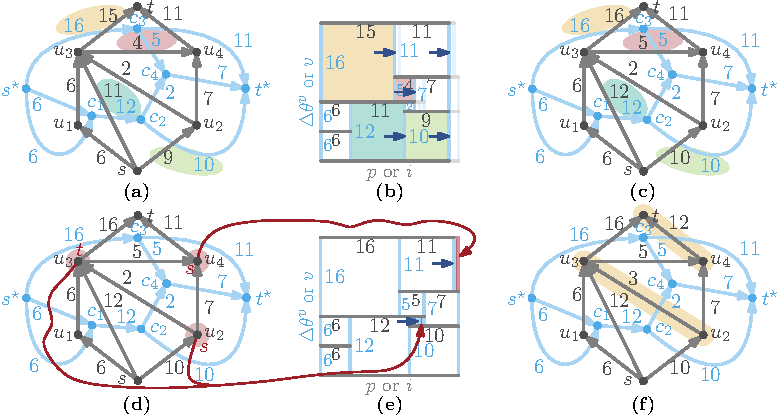
\includegraphics{networkAnalyzes/figures/geometric-interpretation-of-a-kcl-conflict.pdf}
    %
    \caption[KCL Conflict Resolution.]{A \textcolor{PRIMALGRAPH}{primal
    graph~\glssymbol{graph}} and its \textcolor{DUALGRAPH}{dual
    graph~\glssymbol{dualgraph}} that have each six vertices, nine edges, one
    source and one sink are shown in (a), (c), (d), and (f). A geometrical
    representation of both graphs is given in (b) and (e). Each edge in either
    graphs represents a line segment in the appropriate color and the flow on an
    edge defines the aspect ratio of a rectangle, \eg, the
    edges~$\textcolor{DUALGRAPH}{(\cycle_3,\sink^\star)}$ and~$
    \textcolor{PRIMALGRAPH}{(\vertexa_4,\sink)}$ describe
    the~\textcolor{DUALGRAPH}{height} and~\textcolor{PRIMALGRAPH}{width} of the
    upper right rectangle, respectively. (a) A change in flow in the dual graph
    causes a mapping, which effect is shown in (b) and (c). (b) The mapping
    causes a rescaling of some rectangles sides, \ie, in this case the width of
    four rectangles are changed. The outer hull changes from a rectangle to a
    non-rectangle (shown in the background). (c) After the mapping step the
    one-to-one-correspondence is retained. (d) In this case the mapping result
    in a~\gls{kcl} conflict (red) in the primal
    graph~\textcolor{PRIMALGRAPH}{\gls{graph}}. (e) Resizing the two rectangles
    resolves the conflict. (f) The flow on the edges~$(\vertexa_2,\vertexa_3),
    (\vertexa_4,\sink)\in\glssymbol{edges}(\glssymbol{graph})$ resolves the
    conflict. }
    % 
    \label{ch:network-analyzes:sec:algorithm:fig:geometric-interpretation-of-a-kcl-conflict}
\end{figure}
% 
% 
\begin{definition}[Minimal Conflict Resolution]
    % 
    The shortest path~$\glssymbol{path}_{\gls{spp}}$ and the longest
    path~$\glssymbol{path}_{\gls{lpp}}$ are defined by~$
    % 
        \fpath{\gls{spp}}{\source}{\sink}
        \coloneqq
        \argmin_{ \fpath{}{\source}{\sink} \in \glssymbol{pathset} } 
        \sum_{\edge\in\fpath{}{\source}{\sink}}
        \nicefrac{
            \glssymbol{flow}(\edge)
        }{
            \glssymbol{susceptance}(\edge)
        }
    % 
    $ with a length of $
        % 
        \glssymbol{voltageangledifference}(\fpath{\gls{spp}}{\source}{\sink})
        % 
    $ and~$
        % 
        \fpath{\gls{lpp}}{\source}{\sink}
        \coloneqq \argmax_{\fpath{}{\source}{\sink} \in \glssymbol{pathset} } 
        % 
    $ 
    % 
    $
    % 
        \sum_{\edge\in\fpath{}{\source}{\sink}}
        \nicefrac{\glssymbol{flow}(\edge)}{\glssymbol{susceptance}(\edge)}
    % 
    $ with a length of $
        % 
        \glssymbol{voltageangledifference}(\fpath{\gls{lpp}}{\source}{\sink})
        % 
    $, respectively. A conflict resolution in one graph causes a flow change in
    either graphs and thus, the minimum conflict resolution is defined
    in~\glssymbol{graph} and~\glssymbol{dualgraph} by:
    % 
    \begin{compactenum}[\hspace*{1cm}(CR--1)]
    % 
    \item
    Let~$\fpath{\gls{spp}}{\source^\star}{\sink^\star},\fpath{\gls{lpp}}{\source^\star}
    {\sink^\star}\in\glssymbol{pathset}(\glssymbol{dualgraph})$ then a conflict
    resolution in~$\glssymbol{dualgraph}$ is of minimum size if and only
    if~$    
        % 
        \glssymbol{voltageangledifference}(
            \fpath{\gls{spp}}{\source^\star}{\sink^\star}
        ) 
        = 
        \glssymbol{voltageangledifference}(
            \fpath{\gls{lpp}}{\source^\star}{\sink^\star}
        )
        % 
    $.
    % 
    \label{ch:network-analyzes:CR:1}
    % 
    \item
    Let~$
        % 
        \fpath{\gls{lpp}}{\source}{\sink}
        \in
        \glssymbol{pathset}(\glssymbol{graph})
        % 
    $, and
    let~$
        % 
        \glssymbol{voltageangledifference}'(
            \glssymbol{path}_{\gls{lpp}}(\source,\sink)
        )
        % 
    $ and~$
        % 
        \glssymbol{voltageangledifference}(
            \glssymbol{path}_{\gls{lpp}}(\source,\sink))
        % 
    $ be the longest path before and after the change. Then a conflict
    resolution in~$\glssymbol{graph}$ is minimum if and only if the change of
    the longest path~$
    % 
    \Delta_{\gls{lpp}}(\source,\sink)
    \coloneqq
    \glssymbol{voltageangledifference}'(\glssymbol{path}_{\gls{lpp}}(\source,\sink))
    -
    \glssymbol{voltageangledifference}(\glssymbol{path}_{\gls{lpp}}(\source,\sink))
    % 
    $
    is minimized~$
    \min\Delta_{\gls{lpp}}(\source,\sink)
    $.
    % 
    \label{ch:network-analyzes:CR:2}
    % 
    \end{compactenum}
    % 
    We call a conflict resolution minimum if and only
    if~\mbox{CR--\ref{ch:network-analyzes:CR:1}} and
    \mbox{CR--\ref{ch:network-analyzes:CR:2}} holds.
    % 
    \label{ch:network-analyzes:CR}
    % 
\end{definition}
% 
% \begin{proof}
    The conflict resolution~CR--\ref{ch:network-analyzes:CR:1} does not change
    the length of the longest path, but adjusts the length of the shortest path
    to the longest path resulting in a~\gls{kvl} feasible flow. The only
    conflict resolution that changes the length of the longest path
    is~CR--\ref{ch:network-analyzes:CR:2}. However, this represents the smallest
    possible change, since we chose the smallest change of the longest path
    among all choices of changes.% \end{proof}

This can be formulated as an~\gls{lp}, where~CR--\ref{ch:network-analyzes:CR:2}
is an objective and~CR--\ref{ch:network-analyzes:CR:1} is a constraint.
CR--\ref{ch:network-analyzes:CR:1} is illustrated
in~\cref{ch:network-analyzes:sec:algorithm:fig:geometric-interpretation-of-a-kcl-conflict}\screen{d--f},
where the width of the outer rectangle does not change, which is equivalent to
not changing longest path. CR--\ref{ch:network-analyzes:CR:2} is shown
in~\cref{ch:network-analyzes:sec:algorithm:fig:geometric-interpretation-of-a-kcl-conflict}\screen{a--c},
where we solved a conflict in the dual graph~\glssymbol{dualgraph}, which leads
in the mapping step to a change of the width (\ie, change in the longest path of
the primal graph~\glssymbol{graph}).
% 
We now use the aforementioned definition (see~\cref{ch:network-analyzes:CR}) for
a minimum conflict resolution to formulate an algorithm for the conflict
resolution step~\resolveConflict{$\subgraph,
\excessSet, \source, \sink,$ $\glssymbol{flow}_{\subgraph}$}. The set
of~\gls{kcl} conflicts is given by~$
    % 
    \excessSet 
    \coloneqq 
    \{
        \vertexa
        \in
        \glssymbol{vertices}(\subgraph)
        \mid
        \glssymbol{netflow}(\vertexa)
        \neq 
        0
    \}
    % 
$, where~\subgraph is either~\glssymbol{graph} or~\glssymbol{dualgraph}. The
conflict resolution CR--\ref{ch:network-analyzes:CR:1} implies that the edges
for the conflict resolution should lie on
path~$
    % 
    \fpath{ }{\source^\star}{\sink^\star}
    % 
$ with~$
    % 
    \fpath{ }{\source^\star}{\sink^\star} 
    < 
    \fpath{ \gls{lpp} }{\source^\star}{\sink^\star}
    % 
$ of~$
    % 
    \subgraph^{\star} 
    =
    \algoDualGraphOf(\subgraph, \source, \sink)
    % 
$. Thus, a possibility is to compute the shortest path graph
in~$\subgraph^\star$. We save all edges in a set of candidate
edges~$\glssymbol{edges}'$.
% 
% Since the length of~$\fpath{\gls{lpp}}{\source}
% {\sink}$ should not change, but the length of~$\fpath{\gls{spp}}{\source}
% {\sink}$ should be adjusted to the length of the longest path, it suffices to
% select two terminals. 
% 
We define excesses accordingly by~$
    % 
    \source, 
    \vertexa_{\source} 
    \in 
    T_{\source}
    % 
$ and~$
    \sink, 
    \vertexa_{\sink} 
    \in
    T_{\sink}
$.

The conflict resolution~CR--\ref{ch:network-analyzes:CR:2} corresponds to a
minimum change of the longest path in~\subgraph. We have to evenly distribute
the flow excess at each vertex~$
    % 
    \vertexa
    \in
    \excessSet
    \subseteq
    \glssymbol{vertices}
    % 
$ along all paths. Since we wish to minimize~$
    % 
    \Delta_{\gls{lpp}}(\source,\sink)
    \coloneqq
    \glssymbol{voltageangledifference}(\glssymbol{path}_{\gls{lpp}}'(\source,\sink))
    -
    \glssymbol{voltageangledifference}(\glssymbol{path}_{\gls{lpp}}(\source,\sink))
    % 
$, we increase the flow only at edges on the shortest paths~$
    % 
    \fpath{\gls{spp}}{\source'}{\sink'}
    % 
$ in the dual graph until either~$\source'$ or~$\sink'$ are saturated.

We augment iteratively one unit of flow along the shortest~\source-\sink-path
from~$
    % 
    \source' 
    \in 
    T_{\source}\setminus\source
    % 
$ to~$
    % 
    \sink' 
    \in 
    T_{\sink}\setminus\sink
    % 
$ using the metric~$
    % 
    \nicefrac{
        \glssymbol{flow}
    }{
        \glssymbol{susceptance}
    }
    % 
$ until all~$
    % 
    \source'
    \in 
    T_{\source}, 
    \sink'
    \in 
    T_{\sink}
    % 
$ have~$\glssymbol{netflow}(\vertexa) = 0$ with~$
    % 
    \vertexa
    \in
    (
        T_{\source}
        \cup 
        T_{\sink}
    )
    \setminus
    \{\source,\sink\}
    % 
$.
% 
% The sweep line algorithm~$\sweepLineFlowAlgorithm(\vertexa,\glssymbol{netflow}
% (\vertexa),\subgraph', \glssymbol{flow})$
% (see~\cref{ch:network-analyzes:algo:sweepline-algorithm}) is a simple
% modification of a~\gls{bfs} along the shortest path graph from u to t' and
% at each vertex in the BFS we split the flow according to the number of
% outgoing incident edges
% (see~\cref{ch:network-analyzes:algo:sweepline-algorithm}
% in~\cref{ch:network-analyzes:algo:sweepline-algorithm:split}).
% 
% \begin{algorithm}[tb!]%
% \SetAlgoLined
% %%%%%%%%%%%%%%%%%%%%%%%%%%%%%%%%%%
% % 
% \KwData{A directed \source-\sink-graph~$\subgraph$, one source~$\source$, one
% sink~$\sink$, an initial excess~$e'$, and flows~$\glssymbol{flow}
% (\vertexa,\vertexc)$ with~$(\vertexa,\vertexc)\in\glssymbol{edges}$.}%
% \KwResult{Modified flow~$\glssymbol{flow}(\vertexa,\vertexc)$ for all $
% (\vertexa,\vertexc)\in\glssymbol{edges}(\subgraph)$.}
% % 
% % INITIALIZATION %%%%%%%%%%%%%%%%%%%%%%%%%%%%%%%%%%%%%%%%%%%%%%%%%%%%%%%%%%%%
% $\netflow(\vertexa) = e'$\; % vertexa is initial source
% % 
% % LOOP UNTIL QUEUE IS EMPTY %%%%%%%%%%%%%%%%%%%%%%%%%%%%%%%%%%%%%%%%%%%%%%%%%
% \While(\Comment*[f]{\color{KITblack30}Sweep line Resolution of a~\gls{kcl}
% conflict for an~\source-\sink-pair in~\subgraph})% basically a simple BFS search
% % BFS search
% {$\mathcal{Q}\not=\emptyset$}
% { % while
%     $\vertexa = \mathcal{Q}.\deleteFirst()$\;
%     $\flow(\vertexa,\vertexc)
%             = 
%             \flow(\vertexa,\vertexc)
%             + 
%             \frac{\lceil\netflow(\vertexa)\rceil}{\fmagnitude{\outneighbor(\vertexa)}} 
%             \qquad\forall 
%             \vertexc\colon(\vertexa,\vertexc)\in\edges(\subgraph)$\;
%             \label{ch:network-analyzes:algo:sweepline-algorithm:split}
%     % 
%     $\mathcal{Q}.\pushBack(\vertexa)\qquad\forall\vertexa\in\outneighbor
%     (\vertexa)$\;
% }
% 
% %%%%%%%%%%%%%%%%%%%%%%%%%%%%%%%%%%
% \caption{\texttt{sweepLineFlowAlgorithm}}%
% \label{ch:network-analyzes:algo:sweepline-algorithm}%
% \end{algorithm}% 
% 
\begin{conjecture}
    \Cref{ch:network-analyzes:algo:s-t-power-flow-algorithm} computes a
    correct \source-\sink electrical flow of minimum integral size.
    % 
    \label{ch:network-analyzes:lem:minimum-integer-flow}%
\end{conjecture}
% 
% \begin{proof}
We give an idea how we think the proof could work.
% 
    Let~$\glssymbol{flow}(\edge)$ be a minimal integral electrical flow. Let~$
    \glssymbol{flow}'(\edge)$ be some flow with~$ %
        \glssymbol{flow}'(\edge) 
        \leq 
        \glssymbol{flow}(\edge)
        % 
    $ for all~$\edge\in\glssymbol{edges}$ and the flow~$\glssymbol{flow}'$
    fulfills the~\gls{kvl}. We claim that there is a~$
        % 
        \glssymbol{flow}''(\edge)
        =
        \glssymbol{flow}(\edge)
        % 
    $ for all~$\edge\in\glssymbol{edges}$. Assume that there is an edge~$
        % 
        \glssymbol{flow}''(\vertexa,\sink) 
        = 
        \glssymbol{flow}'(\vertexa,\sink) 
        + 1
        >
        \glssymbol{flow}(\vertexa,\sink) 
        % 
    $ meaning the flow would skip a minimal integral solution. This would mean
    that there is another path from~\vertexa to~\sink with~$
    \glssymbol{flow}'''$. Since~$
        % \glssymbol{flow}'(\vertexa,\sink) 
        % = 
        \min_{\fpath{}{\vertexa}{\sink}\in\glssymbol{pathset} } 
        \sum_{(\vertexa,\vertexb)\in\fpath{}{\vertexa}{\sink}}
        \frac{ 
            \glssymbol{flow}(\vertexa,\vertexb) 
        }{ 
            \glssymbol{susceptance}(\vertexa,\vertexb) 
        }
        =
        \min_{\fpath{}{\vertexa}{\sink}\in\glssymbol{pathset} } 
        \sum_{(\vertexa,\vertexb)\in\fpath{}{\vertexa}{\sink}}
        \glssymbol{voltageangledifference}(\vertexa,\sink)
    $ this represents a contradiction.

    % We proof the correctness of the lemma by induction. 
    % 
    We assume that the conjecture is correct for any \source-\sink plane
    graph~\glssymbol{graph} as long as~\glssymbol{graph} constitutes an
    electrical flow. Assuming a graph with~$
    \fmagnitude{\glssymbol{undirectededges}} = 1$ then applying a flow
    of~$\glssymbol{flow}(\source,\sink) = 1$ along an edge incident to~\source
    (which is here the only edge~$ (\source,\sink)$) results in a feasible
    flow~$\glssymbol{flow}_{\glssymbol{graph}}$ in~$\glssymbol{graph}$ and in a
    feasible flow~$\glssymbol{flow}_{\glssymbol{dualgraph}}$
    in~$\glssymbol{dualgraph}$ accordingly.

    Now, we assume an arbitrary \source-\sink plane graph~\glssymbol{graph}. The
    construction of the graph is correct
    (see~\cref{ch:network-analyzes:sec:planar-embedding-dual-graph-construction}).
    Since we resolve each conflict optimal meaning using the minimum number of
    changes in each conflict resolution (see~\cref{ch:network-analyzes:CR}) and
    we push only flow in the predefined direction, we get an order of increasing
    flows and using the minimum conflict resolution does not skip a solution.
    Since we know that
    \glssymbol{graph} has an electrical flow the algorithm terminates.
    % 
    % \franzi{This whole thing reminds me on Benders decomposition, structure is
    % very similar. (Maybe) establish connection to it. }
    % 
    % 
% \end{proof}
% 
% The algorithm terminates in polynomial time, since~\gls{dc}~\gls{feas}
% constitutes a rational polytope this is proven
% in~\cref{ch:network-analyzes:sec:mathematical-model:lem:integral-e-flow-poly-size}.
% 

% 
% Superposition and scaling gives us an electrical flow for multiple sources and
% sinks.
% 
% For Max power flow maybe dynamic programming.
% 
% \begin{figure}
%     % 
%     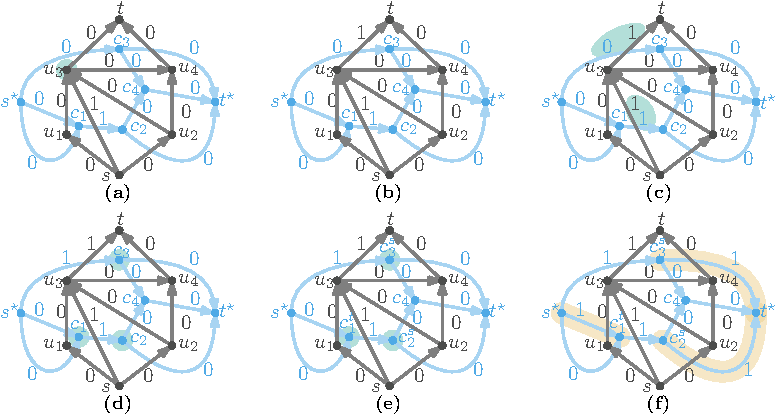
\includegraphics{networkAnalyzes/figures/AlgorithmicSteps.pdf}
%     % 
%     \caption[Example that shows the main steps of the algorithm.]{An example
%     showing the main steps of the algorithm to compute a
%     electrical flow~\glssymbol{flow} on a graph~\glssymbol{graph}. Note that
%     this is the exact same example provided by~\textcite[p.18]{Fel13}. (a)
%     Augmenting~$1$ unit along the shortest path from~\source to~\sink. (b)
%     Mapping step with~$\glssymbol{flow}_{\glssymbol{dualgraph}}(\edge) =
%     \glssymbol{flow}_{\glssymbol{graph}} (\oneToOneMap(\edge))$ for
%     all~$\edge\in\glssymbol{edges}$. (c) \gls{kcl} conflict
%     meaning~$\glssymbol{netflow}(\vertexa)\neq 0$ for
%     some~$\vertexa\in\glssymbol{vertices}$. (d) Define temporary sources and
%     sinks. (e) Compute flow from~$\glssymbol{generators}\coloneqq
%     \{\source,\vertexa_{\source},\vertexb_{\source}\}$
%     to~$\glssymbol{consumers}\coloneqq\{\vertexc_ {\sink},\sink\}$, where
%     temporary terminals have fixed demand and supply. (f) Resulting electrical
%     flow~\glssymbol{flow}.
%     % 
%     }
%     % 
%     \label{ch:network-analyzes:sec:mathematical-model:fig:algorithm}%
% \end{figure}
% 
%%%%%%%%%%%%%%%%%%%%%%%%%%%%%%%%%%%%%%%%%%%%%%%%%%%%%%%%%%%%%%%%%%%%%%%%%%%%%%%%
\section{Conclusion}
% \label{}
%%%%%%%%%%%%%%%%%%%%%%%%%%%%%%%%%%%%%%%%%%%%%%%%%%%%%%%%%%%%%%%%%%%%%%%%%%%%%%%%
% 
This chapter provides a thorough analysis of electrical flows. In the beginning,
we showed different properties of electrical flows as well as methods that are
essential in the first place to design an electrical flow algorithm for planar
graphs and matroids. We give a first algorithm for~\source-\sink electrical
flows that uses electrical preserving transformations and has a running time
of~$
    % 
    \bigO(\fmagnitude{\glssymbol{vertices}}^3)
    % 
$. This is better than the known exponential time algorithm mentioned
in~\cref{ch:network-analyzes:sec:mathematical-model:lem:current_edge_from_a_to_b}.
Even though both algorithms are constructive and exploit some structure, there
is a comparable computation of electrical flows that needs polynomial time for
arbitrary networks. To give electrical flows more structure, we present
different graph-theoretic representations. These representations help us to
separate the quadratic relationship and lead to the balancing property, which
will be used in an algorithmic approach that computes~\source-\sink electrical
flows by using two graphs that are dual
(see~\cref{ch:network-analyzes:sec:algorithm}).

There are still some open conjectures and research questions that we would like
to investigate. One of the first questions, we try to investigate is the running
time and correctness of~\cref{ch:network-analyzes:algo:s-t-power-flow-algorithm}
that depends on the unknown minimum integral generation and demand vector. For
arbitrary susceptances~\glssymbol{susceptance} the resolution can have
exponential size. However, if we restrict the resolution to some ratio, we might
be able to restrict the vector and the running time.

Recall that one assumption on our graphs is that they are planar. On general
graphs that cannot be embedded planar on a plane surface (\ie, surface with
genus 0), we do not have the concept of faces. However, if we chose a surface
with higher genus that allows a plane embedding of the graph, we can make use of
the aforementioned algorithms. Thus, we raise the following conjecture.
% 
\begin{conjecture}
    % 
    \footnote{We thank Peter Sanders for the discussion on that topic. In
    addition, we like to thank Thomas William Brown for mentioning and
    describing Cohomology to us.}
    % 
    \Cref{ch:network-analyzes:algo:s-t-power-flow-algorithm} or the algorithm
    from~\cref{ch:network-analyzes:sec:mathematical-model:thm:algo-pf-1}
    are~\gls{fpt} in the genus.
    % 
\end{conjecture}
% 
We note that computing all~\source-\sink electrical flows, adding them, and
scaling them leads to a multi-source multi-sink electrical flow algorithm that
is not very efficient. Though it might be in general inefficient, it is worth
investing these algorithms for dynamic power grids that make use of the
\source-\sink-decompositions while starting with some initial electrical flow.
%
%%%%%%%%%%%%%%%%%%%%%%%%%%%%%%%%%%%%%%%%%%%%%%%%%%%%%%%%%%%%%%%%%%%%%%%%%%%%%%%%
% \chapter[Discrete Control Units]{Discrete Control Units\footnote{This
% chapter is partly published in~\parencite{Gra18}.}}
\Chapter{Discrete Control Units}{Switching -- A Temporary Removal
of Links and
Cables}{\hspace{2mm}\footnote{This chapter is partly published in~
\parencite{Gra18}.}}
\label{ch:switching}
\glsresetall
% Switching in Power Grids
%%%%%%%%%%%%%%%%%%%%%%%%%%%%%%%%%%%%%%%%%%%%%%%%%%%%%%%%%%%%%%%%%%%%%%%%%%%%%%%%
%
Future power grids will change towards efficient and environmentally friendly
energy operation while handling increasing demands and renewable energy
sources~\parencite{969970}. Renewable energy sources are often added to the
medium and low voltage layer, leading to a bidirectional power flow which the
power grid was not originally designed for. The bidirectional flow dynamically
causes new critical lines and instabilities in the power grid and this effect is
amplified by the increasing demand.
% 
Thus, the network operators have to adapt their power grid to the new challenges
by either expanding it (\ie, adding lines) or operating it more efficiently and
flexibly by adding control units.

This leads to the \emph{dynamic} and \emph{static transmission design
problem}~\parencite{Bin01a}. Dynamic transmission
design~\parencite{Gal92,Cho06,Bin01a} is a long-term power grid configuration
denoted by~\acrlong{tnep}~(\gls{tnep}) that adds new transmission lines and
circuits to the existing power grid. Although adding lines to the power grid
decreases the aggregated grid resistance~\parencite{Pot12,Cof14a}, it may
decrease the operational limit (\ie, a state of power grid congestion is reached
earlier).
%
However, it is hard to determine the best power grid topology over a long
time horizon for different scenarios. Thus, a subproblem of the dynamic design
%
problem---though less expensive---is the static design problem, which
considers the placement of new electrical devices and represents a short-term
solution.

For the latter, devices such as circuit breakers (known as~\emph{switches})
or~\gls{facts} (\acrlong{facts}) are able to manipulate the power flow by
opening a circuit (switching a line off) or routing a certain fraction of power
by changing the susceptance at a transmission line, respectively. Switches
and~\gls{facts} do not intrinsically cause security and reliability
problems~\parencite{LiG13}. However, they are able to reduce the generation
costs, while still satisfying the~$N-1$ criterion (\ie, power grid elements
remain in operation while one element is removed or has a failure)
% 
and extending the operability~\parencite{Bin01b,Lei15b,LiG13}. While
transmission system operators~(\gls{tso}{s}) already use switching in certain
cases of emergency to decouple parts of the grid, avoid abnormal voltage
conditions or improve voltage profiles~\parencite{Fis08}, it is not used to
extend the operability of the grid or reduce costs and losses,
since~\gls{tso}{s} wish to interfere as little as possible with the power
grid~\footnote{From a conversation with the~\gls{tso} TransnetBW.}. However,
these interventions are mainly done by rules of thumb, experience or ad-hoc
reactions. Our approach tries to structure and improve these interventions.

Note that the reliability of the power grid is very important and one would
intuitively assume that only~\gls{tnep} can maintain the power grid's
reliability and efficiency. However, both switches and~\gls{facts} provide
possible control methods for over- and under-voltage situations, line
overloads~\parencite{Gra06}, loss and cost reductions~\parencite{Sch90},
improving system security~\parencite{Sch88}, and combinations of
all~\parencite{Hed11}.
% % 
In addition, in~\cref{ch:facts} we show that placing \emph{ideal}~\gls{facts}
such that the remaining graph is a cactus or tree gives us a
% 
cost-equivalent power flow to the minimum cost flow representing a global
optimum. Furthermore, the results in~\cref{ch:facts} show that placing
ideal~\gls{facts} in the power grid often increases the operability while
lowering the costs. Similar observations were made for
switching~\parencite{Hedman2011}.
%
Note that ideal~\gls{facts} are more powerful than a combination
of~\gls{facts} and switches as they can control the power flow without
limitations.

In contrast to~\gls{facts} and~\gls{tnep}, transmission switching is a
cost-effective way to implement controllability~\parencite{7764210} while using
the existing power grid. Most efficiency gains arise while switching branches
during peak periods~\parencite{6069831} though efficiency is not part of the
objective.
% 
Focusing on increasing the operability during peak periods leads towards
the~\acrlong{mfp}~(\gls{mfp}) and in terms of power grids towards
the~\acrlong{mpfp}~(\gls{mpfp}). Note that the gap between the~\acrlong{mpf}
(\gls{mpf}) and~\acrlong{mf}~(\gls{mf}) can be large as~\acrlong{kvl}
(\gls{kvl}) restricts the flow on cycles. Adding switches decreases the gap and
leads to the~\acrlong{mtsfp}~(\gls{mtsfp}).
\gls{mtsfp} tries to use switches to maximize the possible network capacity.
Networks with more available capacity are more
reliable~\parencite{hedman2010optimal}.
% 
Note that~\gls{ac}-feasibility (\ie, deciding whether there is a generator
dispatch such that the demand can be satisfied) is already~\NP-hard on
trees~\parencite{Leh16}. Thus, we use a linearization of the~\gls{ac} power
flow, denoted by~\gls{dc} power flow
(see~\cref{ch:foundations:sec:power-flow-analyses:subsec:Lin-DC-Model}), where
the feasibility is easy to decide. However, \gls{mtsfp} using~\gls{dc} is
% 
already~\NP-hard (see~\cref{ch:switching:sec:complexity}).
% 
%%%%%%%%%%%%%%%%%%%%%%%%%%%%%%%%%%%%%%%%%%%%%%%%%%%%%%%%%%%%%%%%%%%%%%%%%%%%%%%
\section[A Mathematical Model for the Placement of Discrete Control Units]{
A Mathematical Model for the \protect\linebreak{Placement of Discrete Control Units}} 
% 
\label{ch:switching:sec:model}
%%%%%%%%%%%%%%%%%%%%%%%%%%%%%%%%%%%%%%%%%%%%%%%%%%%%%%%%%%%%%%%%%%%%%%%%%%%%%%%
% 
The general feasibility models were introduced in~\cref{ch:foundations} and a
deeper discussion of the~\gls{dc} feasibility problem was given
in~\cref{ch:network-analysis}. The problem we introduce in this section is a
Combinatorial Optimization Problem. Note that an optimal solution for switching
problems is a subset of the edges~\glssymbol{edges}, where the
set~\glssymbol{edges} of edges represents the set of transmission lines,
transformers, phase shifters, and other line-based electrical equipment in a
power grid. Every undirected graph can be represented by a directed graph by
replacing an undirected edge by two directed edges in either direction. The
latter is called a~\emph{bidirected graph}.
% 
Let~$
\glssymbol{graph}
% 
= 
% 
(
% 
\glssymbol{vertices},
% 
\glssymbol{edges}
% 
)
$ be a bidirected graph with
a set of
vertices~\glssymbol{vertices} (also called buses) representing generator
vertices~$
\glssymbol{generators}
% 
\subseteq
\glssymbol{vertices}$, consumer
vertices~$
\glssymbol{consumers}
% 
\subseteq
\glssymbol{vertices}$, and intermediate
vertices~$\glssymbol{vertices}\setminus(
\glssymbol{generators}\cup\glssymbol{consumers})$
such
that~$\glssymbol{generators}\cap\glssymbol{consumers}=\emptyset$.
%
For simplicity, we use~$
% 
\glssymbol{undirectededges}
% 
$ to denote the underlying undirected
edge set, and for~$\edge\in\glssymbol{edges}$ we denote by~$\undirectededge\in
\glssymbol{undirectededges}$ the underlying undirected edge, \ie, $\undirected{
\vertexa}{\vertexb} = \undirected{\vertexb}{\vertexa}$.
The power grid is modeled as a  
% 
network~$\glssymbol{network} =
(\glssymbol{graph},
\glssymbol{generators},
\glssymbol{consumers},
\glssymbol{capacity}, 
\glssymbol{susceptance}, 
\realpowerdemandmin
% \glssymbol{mindemand}
)$ 
% 
with a capacity function~$\glssymbol{capacity}\colon\edges\to\posreals$
representing the
thermal line limit of an edge, the
susceptance~$\glssymbol{susceptance}\colon\glssymbol{edges}\to\posreals$,
% 
and the demands' lower bounds~$\realpowerdemandmin\colon\consumers\to\posreals$.
% 
%%%%%%%%%%%%%%%%%%%%%%%%%%%%%%%%%%%%% FIGURE %%%%%%%%%%%%%%%%%%%%%%%%%%%%%%%%%%%
\begin{figure}[t!]%
    \centering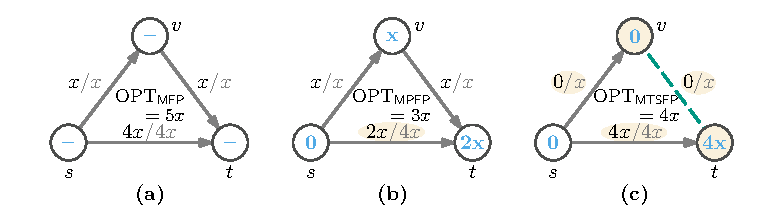
\includegraphics{switchplacement/figures/simple_switching_example_comparing_mf_mpf_mtsf.pdf}
    %
    \caption[A simple switching example that compares~\gls{mf}, 
    \gls{mpf}, and~\gls{mtsf}.]{%
    A network~\glssymbol{network} with three vertices and edges,
    capacities~\screentextcolor{KITblack50}{$\glssymbol{capacity}(\vertexa,\vertexb)$}
    \mbox{(\screentextcolor{KITblack50}{gray})}, one generator~$
    \glssymbol{generators}=\{\source\}$, one consumer~$\glssymbol{consumers} = 
    \{\sink\}$,
    susceptance~$\glssymbol{susceptance} \equiv 1$ for
    all~$(\vertexa,\vertexb)\in\glssymbol{edges}$, and voltage
    angles~\screentextcolor{THETA}{\vangle} (\screentextcolor{THETA}{blue}) for
    electrically feasible flows. The successive differences are marked
    (\hlhili{orange}). (a)~The~$\gls{mfp}(\glssymbol{network})$ is the problem
    that tries to congest all edges and has a value of~$\opt_{\gls{mfp}} = 5x$.
    (b)~The~$\gls{mpfp}(\glssymbol{network})$ with~$\opt_{\gls{mpfp}} = 3x$ is
    restricted by the path with the lowest capacity. (c)~Removing an edge with
    the lowest capacity (\screentextcolor{KITgreen}{dashed line}) helps to
    approach the~\gls{mf}. However, the value of~$\opt_{\gls{mtsfp}}$ is~$4x$. }%
    % 
    \label{ch:switching:sec:model:fig:simple_switching_example}%
\end{figure}%
%%%%%%%%%%%%%%%%%%%%%%%%%%%%%%%%%%%%%%%%%%%%%%%%%%%%%%%%%%%%%%%%%%%%%%%%%%%%%%%%
%

A flow is a function~$\glssymbol{flow}\colon\glssymbol{edges}\to\reals$ that satisfies
the
%
skew-symmetry property~$\glssymbol{flow}(\vertexa,\vertexb) = -\glssymbol{flow}(\vertexb,\vertexa)$
for all~$(\vertexa,\vertexb)\in\glssymbol{edges}$. 
%
Moreover, it has to satisfy the following flow conservation 
property~(\cref{ch:switching:sec:model:eq:flow_conservation,ch:switching:sec:model:eq:unlimited_demand_constraint,ch:switching:sec:model:eq:unlimited_generation_constraints}).
% 
For a vertex~$\vertexa\in\glssymbol{vertices}$ the~\emph{net flow} is denoted
by~$\glssymbol{netflow}(\vertexa) \coloneqq
\sum_{\{\vertexa,\vertexb\}\in\glssymbol{undirectededges}}\glssymbol{flow} 
(\vertexa,\vertexb)$.
%
Similar to~\acrlong{kcl} (\gls{kcl},
see~\cref{ch:switching:sec:model:eq:flow_conservation}) the conservation of flow
describes the flow at each vertex including the consumption or outflow to other
network layers, which is bounded by~$\realpowerdemandmin\geq 0$ and often
denoted as
demand~(\cref{ch:switching:sec:model:eq:unlimited_demand_constraint}), and
the generation limits
(\cref{ch:switching:sec:model:eq:unlimited_generation_constraints}).
%
% %%%%%%%%%%%%%%%%%%%%%%%%%%%%%%%%%%% EQUATIONS %%%%%%%%%%%%%%%%%%%%%%%%%%%%%%%%%%
\begin{align}%
\glssymbol{netflow}(\vertexa) &= 0 & \forall\vertexa\in
\glssymbol{vertices}\setminus
(\glssymbol{generators}\cup\glssymbol{consumers}),
\label{ch:switching:sec:model:eq:flow_conservation}\\%
%
-\infty\leq\glssymbol{netflow}(\vertexa) &\leq-\realpowerdemandmin(\vertexa) &
\forall\vertexa\in\glssymbol{consumers} ,
\label{ch:switching:sec:model:eq:unlimited_demand_constraint}\\%
%
0\leq\glssymbol{netflow}(\vertexa) &\leq \infty &
\forall\vertexa\in\glssymbol{generators}.%
\label{ch:switching:sec:model:eq:unlimited_generation_constraints}%
\end{align}%
%
A flow~\glssymbol{flow} is~\emph{feasible} if it obeys the thermal limits given
by the capacity constraints
(\cref{ch:switching:sec:model:eq:capacity_constraints}).

\begin{equation}%
  \fmagnitude{\glssymbol{flow}(\vertexa,\vertexb)}\leq\glssymbol{capacity}
  (\vertexa,\vertexb)
  \qquad\forall(\vertexa,\vertexb)\in\glssymbol{edges}.
  % 
  \label{ch:switching:sec:model:eq:capacity_constraints}%
\end{equation}%
% 
The~\emph{flow value}~$\glssymbol{flowvalue}(\glssymbol{network},\glssymbol{flow})$ of a
flow~\glssymbol{flow} on~\glssymbol{network} is defined
by~$\sum_{\vertexa\in\glssymbol{generators}}\glssymbol{netflow}(\vertexa)$. A
feasible flow~\glssymbol{flow} on~\glssymbol{network}
maximizing~$\glssymbol{flowvalue}(\glssymbol{network},\glssymbol{flow})$ is
called a~\acrlong{mf}~(\gls{mf}) and the problem of finding such a flow is
denoted by~$\gls{mfp}(\glssymbol{network})$. Its value is denoted
by~$\opt_{\gls{mfp}}(\glssymbol{network}) \coloneqq \max_{\glssymbol{flow}}
\glssymbol{flowvalue}(\glssymbol{network},\glssymbol{flow})$
(see~\cref{ch:switching:sec:model:fig:simple_switching_example}\screen{a}).%

However, a feasible flow neglects some physical constraints of a power flow
denoted as~\acrlong{kvl} (\gls{kvl}, \cref{ch:switching:sec:model:eq:KVL_dc_approx}).
%
%%%%%%%%%%%%%%%%%%%%%%%%%%%%%%%%%%% EQUATIONS %%%%%%%%%%%%%%%%%%%%%%%%%%%%%%%%%
\begin{align}%
  \glssymbol{susceptance}(\vertexa,\vertexb)\cdot (\glssymbol{voltageangle}(\vertexa) - \glssymbol{voltageangle}(\vertexb) -
  \glssymbol{voltageangleshift}(\vertexa,\vertexb)) &= \glssymbol{flow}(\vertexa,\vertexb)
  &\hspace*{-2mm}\forall
  (\vertexa,\vertexb)&\in\glssymbol{edges},%
  \label{ch:switching:sec:model:eq:KVL_dc_approx}%
  \\
  %
  \vanglemin(\vertexa) 
  \leq \hspace*{1.4mm}\glssymbol{voltageangle}(\vertexa)\hspace*{1.3mm} &
  \leq \vanglemax(\vertexa)&\forall\vertexa&\in\glssymbol{vertices},%
  \label{ch:switching:sec:model:eq:theta_bound}%
\end{align}%
% 
where the voltage angle is a
function~$\glssymbol{voltageangle}\colon\glssymbol{vertices}\to\reals$
describing the potential at each vertex. In general, absolute voltage angles are
used, \ie, the angle of one vertex---often the slack---is set to zero and the
others are determined from it~\cite[see][p. 40]{bollobas1998modern}. A deeper
discussion of the latter is available
in~\cref{ch:network-analyzes:sec:mathematical-model}. The voltage
angle~$\glssymbol{voltageangle}(\vertexa)$ of a
vertex~$\vertexa\in\glssymbol{vertices}$ is often limited
to~$\fmagnitude{\glssymbol{voltageangle}(\vertexa)}\leq 0.6$~radians
(see~\cref{ch:switching:sec:model:eq:theta_bound}) to improve the running
time~\parencite{Fis08,6345550}, but this may result in non-optimal solutions or
no solution at all. Note that the voltage angle differences are already covered
by the capacity
constraint~(\cref{ch:switching:sec:model:eq:capacity_constraints}) and thus, the
constraint is not mentioned here. In addition, in most~\gls{ieee} examples and
related works~$\glssymbol{voltageangleshift}\equiv 0$ representing the
transformer (phase shifter) final angle. The latter means that we assume to have
neither~\gls{facts} nor phase shift transformers on the lines. Thus, we neglect
them in the following.
% 
%%%%%%%%%%%%%%%%%%%%%%%%%%%%%%%%%%%%% FIGURE %%%%%%%%%%%%%%%%%%%%%%%%%%%%%%%%%%%
\begin{figure}[t!]%
    \centering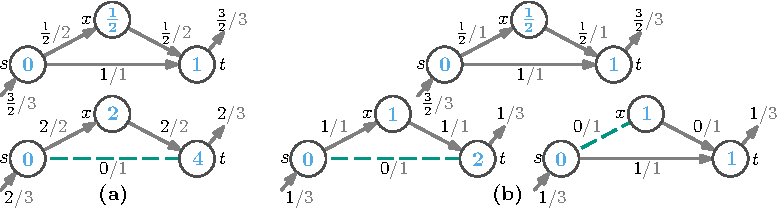
\includegraphics{switchplacement/figures/not_benefitial_simple_switching_example.pdf}
    %
    \caption[The Braess's Paradox highly depends on the network's parameters.]{%
    The Braess's Paradox highly depends on the network's parameter. A general
    observation on that was already given by~\textcite{Pas97}. This example
    network consists of three vertices, three edges, one generator, one load,
    susceptances~$\glssymbol{susceptance} \equiv 1$, and different capacity~$
    \textcolor{CAPACITY}{\glssymbol{capacity}(\edge)}$ settings
    (\textcolor{CAPACITY}{gray}) for all~$\edge\in\glssymbol{edges}$. (a) The
    capacities are chosen in such a way that switching is beneficial in that
    particular network~\glssymbol{network}. The~\gls{mpfp} has a value
    of~$\opt_{\gls{mpfp}}(\glssymbol{network}) = \nicefrac{3}{2}$, whereas
    the~\gls{mtsfp} has a value of~$\opt_{\gls{mtsfp}}(
    \glssymbol{network}) = 2$. (b) The capacities of the edges~$(\source,x)$
    and~$ (x,\sink)$ are set to~$1$. This small reconfiguration makes switching
    not beneficial anymore, since the~\gls{mpfp} has a value
    of~$\opt_{\gls{mpfp}} = \nicefrac{3}{2}
    =
    \opt_{\gls{mtsfp}}$ and any switching has a value of~$1$. }%
    %
    \label{ch:switching:sec:model:fig:when_switching_is_not_benefitial}%
\end{figure}%
%%%%%%%%%%%%%%%%%%%%%%%%%%%%%%%%%%%%%%%%%%%%%%%%%%%%%%%%%%%%%%%%%%%%%%%%%%%%%%%%
%

We call a feasible flow complying
with~\cref{ch:switching:sec:model:eq:KVL_dc_approx,ch:switching:sec:model:eq:theta_bound}
a \emph{feasible electrical flow}. A feasible electrical 
flow~\glssymbol{flow} on~\glssymbol{network}
% 
%
that maximizes~$\glssymbol{flowvalue}(\glssymbol{network},\glssymbol{flow})$ 
%
is called a maximum power flow~($\gls{mpf}$). The
corresponding problem is called the~\acrlong{mpfp}~(\gls{mpfp}) and is denoted
by~$\gls{mpfp}(\glssymbol{network})$.
%
%
The value of~$\gls{mpfp}(\glssymbol{network})$ is denoted
by~$\opt_{\gls{mpfp}}(\glssymbol{network})$ and is defined
by~$\max_{\glssymbol{flow}}\glssymbol{flowvalue}(\glssymbol{network},
\glssymbol{flow})$
(see~\cref{ch:switching:sec:model:fig:simple_switching_example}\screen{b}).
% 

For a subset~$\glssymbol{switched}\subseteq\glssymbol{undirectededges}$ we
consider the graph~$\glssymbol{graph}-\glssymbol{switched}$ and the
corresponding network~$\glssymbol{network}-\glssymbol{switched}$ where the
functions~\glssymbol{capacity} and~\glssymbol{susceptance} are restricted
to~$\glssymbol{edges}\setminus\glssymbol{switched}$.
%
We call~\glssymbol{switched} the set of switched edges (\ie, the switch is in
OFF-state for these edges). Typically not all possible switchings are feasible.
Feasibility in this context means that there is an electrically feasible flow
in~$\glssymbol{network}-\glssymbol{switched}$.
%
%
The problem of maximizing the flow value in~\glssymbol{network} while allowing
edges to be switched is called~\acrlong{mtsfp}~(\gls{mtsfp}) and its value is
denoted by~$\opt_{\gls{mtsfp}}(\glssymbol{network})
\coloneqq
% 
\max_{\glssymbol{switched}\subseteq\glssymbol{undirectededges}}
\opt_{\gls{mpfp}}(\glssymbol{network}-\glssymbol{switched})$ (see~\cref{ch:switching:sec:model:fig:simple_switching_example}\screen{c}). Such a flow
% 
obeys~\cref{ch:switching:sec:model:eq:flow_conservation,ch:switching:sec:model:eq:unlimited_demand_constraint,ch:switching:sec:model:eq:unlimited_generation_constraints,ch:switching:sec:model:eq:capacity_constraints_switching,ch:switching:sec:model:eq:linearized_switching_geq,ch:switching:sec:model:eq:linearized_switching_leq}. 
% 
Note that switching is not always beneficial as shown in~\cref{ch:switching:sec:model:fig:when_switching_is_not_benefitial}\screen{b}.
%
\begingroup
    %%%%%%%%%%%%%%%%%%%%%%%%%%%%%%%%%%% Problem %%%%%%%%%%%%%%%%%%%%%%%%%%%%%%%%%%%%
\begin{problem}[framed]{\acrlong{mtsfp}~$\gls{mtsfp}(\glssymbol{network})$}%
    Instance: & A network~\glssymbol{network}.\\
    % 
    Objective: & Find a
    set~$\glssymbol{switched}\subseteq\glssymbol{undirectededges}$ of switched
    edges such
    that~$\opt_{\gls{mpfp}}(\glssymbol{network}-\glssymbol{switched})$ is maximum
    among all choices of switched edges~\glssymbol{switched}.
\end{problem}%
    \label{ch:switching:problems:MTSF-Optimization_problem}
\endgroup
%
To model switching an edge we introduce a
function~$\glssymbol{switch}\colon\glssymbol{edges}\to\{0,1\}$, which is~$0$ if
an edge is switched and~$1$ otherwise.
%
To enforce the switching, the flow must be zero on the switched edges. We
therefore replace~\cref{ch:switching:sec:model:eq:capacity_constraints} with
\cref{ch:switching:sec:model:eq:capacity_constraints_switching}. This change is
not yet sufficient, since the KVL
(\cref{ch:switching:sec:model:eq:KVL_dc_approx}) shall only apply to the
non-switched edges. Hence, we modify this equation 
to~\cref{ch:switching:sec:model:eq:KVL_quadratic_switching}.%
%
%%%%%%%%%%%%%%%%%%%%%%%%%%%%%%%%%%% EQUATION %%%%%%%%%%%%%%%%%%%%%%%%%%%%%%%%%%
\begin{align}%
    \hspace*{-2.5mm}b(\vertexa,\vertexb)\!\cdot\! \switch(\vertexa,\vertexb)\cdot 
    (\glssymbol{voltageangle}
    (\vertexa) - \glssymbol{voltageangle}(\vertexb))
    &= \glssymbol{flow}(\vertexa,\vertexb) &\forall 
    (\vertexa,\vertexb)\in\glssymbol{edges},\hspace*{-1mm}
    \label{ch:switching:sec:model:eq:KVL_quadratic_switching}\\%
    %
    \fmagnitude{\glssymbol{flow}(\vertexa,\vertexb)}&\leq 
    \glssymbol{switch}(\vertexa,\vertexb)\cdot
    \glssymbol{capacity}(\vertexa,\vertexb)
    \hspace*{-1mm} &
    \forall(\vertexa,\vertexb)\in\glssymbol{edges}.\hspace*{-1mm}
    % 
    \label{ch:switching:sec:model:eq:capacity_constraints_switching}%
\end{align}%
%
\cref{ch:switching:sec:model:eq:KVL_quadratic_switching} can be linearized by
either adding two big-$M$ constraints
(\cref{ch:switching:sec:model:eq:linearized_switching_geq,ch:switching:sec:model:eq:linearized_switching_leq})
or one indicator constraints
(\cref{ch:switching:sec:model:eq:indicator_constraint}), where~$M$ is a suitably
large constant.
%
\begin{align}%
  \hspace*{-3mm}\glssymbol{susceptance}(\vertexa,\vertexb)\cdot
  (\glssymbol{voltageangle}(\vertexa) - \glssymbol{voltageangle}(\vertexb)) &+
  (1 - \glssymbol{switch}(\vertexa,\vertexb) ) M\geq
  \glssymbol{flow}(\vertexa,\vertexb)\hspace*{-2mm} &\forall
  (\vertexa,\vertexb)\in\glssymbol{edges},\hspace*{-1mm}
  \label{ch:switching:sec:model:eq:linearized_switching_geq}\\%
  %
  \hspace*{-3mm}\glssymbol{susceptance}(\vertexa,\vertexb)\cdot (
  \glssymbol{voltageangle}(\vertexa) - \glssymbol{voltageangle}(\vertexb)) &-
  (1 - \glssymbol{switch}(\vertexa,\vertexb) ) M\leq \glssymbol{flow}(\vertexa,\vertexb)\hspace*{-2mm} &\forall 
  (\vertexa,\vertexb)\in\glssymbol{edges},\hspace*{-1mm}
  \label{ch:switching:sec:model:eq:linearized_switching_leq}\\%
  % 
  \hspace*{-1mm}\glssymbol{switch}(\vertexa,\vertexb) = 1 \Rightarrow \glssymbol{susceptance}
  (\vertexa,\vertexb)\cdot(
  \glssymbol{voltageangle}(\vertexb) - \glssymbol{voltageangle}(\vertexa) )
  &\hphantom{- (1 - \glssymbol{switch}(\vertexa,\vertexb) ) M .} =
  \glssymbol{flow}(\vertexa,\vertexb) &\forall
  (\vertexa,\vertexb)\in\glssymbol{edges}.\hspace*{-1mm}
  \label{ch:switching:sec:model:eq:indicator_constraint}
  % 
\end{align}%
%
The parameter~$M$ must be reasonably large to not impose any implicit voltage
angle difference limit at the edge~$(\vertexa,\vertexb)\in\glssymbol{edges}$. In
general, one can choose~$M$ for each
edge~$(\vertexa,\vertexb)\in\glssymbol{edges}$ by~$M{(\vertexa,\vertexb)}$ equal
to~$\max\left\{\sum_{\edge\in\pi(\vertexa,\vertexb)}\glssymbol{susceptance}(\edge)^{-1}
\glssymbol{capacity} (\edge)\right\}$,
%
%
where the maximum ranges over all simple paths~$\fpath{}{\vertexa}{\vertexb}$
from~\vertexa to~\vertexb. It then suffices to set $M
=\max_{(\vertexa,\vertexb)\in\glssymbol{edges}}M{(\vertexa,\vertexb)}$~
\parencite{Bin01a}. However, it is \NP-hard to calculate the longest path
\parencite{Karger1997}. It is simpler to set~$M(\vertexa,\vertexb) =
\glssymbol{susceptance}(\vertexa,\vertexb) \cdot $
$\sum_{\edge\in\glssymbol{edges}}
\nicefrac{\glssymbol{capacity}(\edge)}
{\glssymbol{susceptance}(\edge)}$. If we restrict the voltage
angle~\glssymbol{voltageangle} to~$0.6$ radians
in~\cref{ch:switching:sec:model:eq:theta_bound}, which is
common~\parencite{6345550,5401077}, we can use~$M{(\vertexa,\vertexb)} =
1.2\cdot\fmagnitude{\glssymbol{susceptance}(\vertexa,\vertexb)}$. Note that this
decreases the solution space and possibly removes feasible and optimal
solutions. Thus, this restriction can improve the running time, but might lead
to other results and is thus debatable, from a physical point of view.
% 
In general, we have lower and upper bounds for
generators~$
\realpowergenerationmin,
\realpowergenerationmax
\colon
\glssymbol{generators}
\to
\posreals
\cup\{\infty\}$,
and demands~$
\realpowerdemandmin,
\realpowerdemandmax
\colon
\glssymbol{consumers}
\to
\posreals
\cup
\{\infty\}$ for~$\vertexa\in\glssymbol{consumers}$ such
that~\cref{ch:switching:sec:model:eq:unlimited_demand_constraint,ch:switching:sec:model:eq:unlimited_generation_constraints}
become~\cref{ch:switching:sec:model:eq:demand_constraint,ch:switching:sec:model:eq:generation_constraints},
respectively, and the network is defined by~$\dcnetworktuple$. A network with
these additional bounds is called~\emph{bounded}.
%
% %%%%%%%%%%%%%%%%%%%%%%%%%%%%%%%%%%% EQUATIONS %%%%%%%%%%%%%%%%%%%%%%%%%%%%%%%%%%
\begin{align}%
  -\realpowerdemandmax(\vertexa)\leq\glssymbol{netflow}(\vertexa) &\leq 
  -\realpowerdemandmin(\vertexa) & \forall\vertexa\in\glssymbol{consumers}
  \label{ch:switching:sec:model:eq:demand_constraint}\\%
  %
  \realpowergenerationmin(\vertexa)\leq\glssymbol{netflow}(\vertexa) &\leq 
  \realpowergenerationmax(\vertexa) & \forall\vertexa\in\glssymbol{generators}
  \label{ch:switching:sec:model:eq:generation_constraints}%
\end{align}%
%
A~$\gls{mtsf}$ obeying the latter constraints is a \emph{bounded~\gls{mtsf}}.
Note that fixing the demands~$\realpowerdemandmin (\vertexa) =
\realpowerdemandmax(\vertexa) = \realpowerdemand(\vertexa)$ and
generations~$\realpowergenerationmin(\vertexa) = \realpowergenerationmax
(\vertexa) = \realpowergeneration(\vertexa)$ leads to
a~\acrlong{dc}~\acrlong{feas} (\gls{dc}~\gls{feas}) also known as~\acrlong{pf}
(\gls{pf}) that is the search for a feasible electrical flow by given demands
and generations. We discussed the latter problem in more detail
in~\cref{ch:network-analysis}.

Suppose every generator~$\vertexa\in\glssymbol{generators}$ has its own
generation cost function~$\gamma_\vertexa\colon\reals\to\posreals$ representing
the cost for generating the power~$\glssymbol{netflow}(\vertexa)$.
%
The problem of minimizing the generation costs of all
generators~$\vertexa\in\glssymbol{generators}$ while maintaining a 
feasible electrical flow in a bounded network with $\realpowerdemandmin(\vertexa) = 
\realpowerdemandmax(\vertexa) = \realpowerdemand(\vertexa)$ (\ie,
% 
\cref{ch:switching:sec:model:eq:flow_conservation,ch:switching:sec:model:eq:capacity_constraints,ch:switching:sec:model:eq:capacity_constraints,ch:switching:sec:model:eq:KVL_dc_approx,ch:switching:sec:model:eq:theta_bound,ch:switching:sec:model:eq:demand_constraint,ch:switching:sec:model:eq:generation_constraints})
% 
is called~\acrlong{opfp}~$\gls{opfp}(\glssymbol{network})$. The
value of~$\gls{opfp}(\glssymbol{network})$ is denoted by~$\opt_{\gls{opfp}}(
\glssymbol{network}) = \min \sum_{\vertexa\in\glssymbol{generators}}
\fcost{\vertexa}(\glssymbol{netflow}(\vertexa))$. The problem of finding
a flow with value~$\opt_{\gls{opfp}}(\glssymbol{network})$
by allowing edges to be switched (\ie,
% 
\cref{ch:switching:sec:model:eq:flow_conservation,ch:switching:sec:model:eq:theta_bound,ch:switching:sec:model:eq:capacity_constraints_switching,ch:switching:sec:model:eq:linearized_switching_geq,ch:switching:sec:model:eq:linearized_switching_geq,ch:switching:sec:model:eq:demand_constraint,ch:switching:sec:model:eq:generation_constraints})
% 
is called~\acrlong{otsp}~$\gls{otsp}(\glssymbol{network})$ with 
value~$\opt_{\gls{otsp}}(\glssymbol{network})=
\min_{\glssymbol{switched}\subseteq\glssymbol{undirectededges}}\opt_{
\gls{opfp}}(
\glssymbol{network}\!-\!
\glssymbol{switched})$ with~$\glssymbol{switched}$ being the set of switched
edges.
% 
\begingroup
    %
%%%%%%%%%%%%%%%%%%%%%%%%%%%%%%%%%%% Problem %%%%%%%%%%%%%%%%%%%%%%%%%%%%%%%%%%%%
\begin{problem}[framed]{\acrlong{otsp}~$\gls{otsp}(\glssymbol{network})$}%
  % 
  Instance: & A network~\glssymbol{network}.\\%
  % 
  Objective: & Find a set~$\glssymbol{switched}\subseteq\glssymbol{edges}$ and
  an electrically feasible flow~\glssymbol{flow} in~$
  \glssymbol{network}-\glssymbol{switched}$ such that the sum of the generation
  costs~$\sum_{\vertexa\in\glssymbol{generators}}\gamma_\vertexa\left(
  \glssymbol{netflow}(\vertexa)\right)$ is minimized.%
  %
\end{problem}%
    \label{ch:switching:problems:OTS-Optimization_problem}
\endgroup
%
Note that neither the~\gls{mtsfp} nor the~\gls{otsp} minimize the number of
switches. This would result in a~$\min$-$\max$-problem  that is harder to solve
than the presented basic variants
(see~\cref{ch:switching:sec:problem-definition} on
Page~\pageref{ch:switching:sec:problem-definition}). From~\textcite[Lemma
4]{Leh15a} it further follows that the~\gls{mtsfp} and
the~\acrlong{mffp}~(\gls{mffp}) are polynomial-time solvable on trees. Thus, for
trees we get the following relationship.
% 
$$\opt_{\gls{mpfp}}(\glssymbol{network}) 
= \opt_{\gls{mtsfp}}(\glssymbol{network})
= \opt_{\gls{mffp}}(\glssymbol{network})
= \opt_{\gls{mfp}}(\glssymbol{network}).
% 
\label{ch:switching:structure:tree}
$$
% 
If it is clear, which network is being referred to, we may omit the explicit
reference~\glssymbol{network} and write~$\glssymbol{problems}$
and~$\opt_{\glssymbol{problems}}$ instead
of~$\glssymbol{problems}(\glssymbol{network})$
and~$\opt_{\glssymbol{problems}}(\glssymbol{network})$,
where~$\glssymbol{problems}$ is a particular problem~(\eg,
\gls{mtsfp}). The common constraints of~\gls{mtsfp} and~\gls{otsp} are the base
constraints for
the~\acrlong{rop}~(\gls{rop})~\parencite{van2011vehicle,COFFRIN2015144}
and~\gls{tnep}~\parencite{Hem13}.
% 
%%%%%%%%%%%%%%%%%%%%%%%%%%%%%%%%%%%%%%%%%%%%%%%%%%%%%%%%%%%%%%%%%%%%%%%%%%%%%%%
\begin{landscape}
    \begin{table}
        % 
        % latex table generated in R 3.2.2 by xtable 1.8-0 package
% Wed Jan 27 11:17:04 2016
% \vspace{-1.5cm}
{\setlength{\tabcolsep}{0.3em}}
{\renewcommand{\arraystretch}{1}}% for the vertical padding
% \footnotesize
\begin{tabular}{
  l>{\centering\arraybackslash}%
  m{1.5cm}>{\centering\arraybackslash}%
  m{3.0cm}>{\centering\arraybackslash}%
  m{1.7cm}cccc>{\centering\arraybackslash}%
  m{2.7cm}>{\centering\arraybackslash}%
  m{2.7cm}>{\centering\arraybackslash}%
  m{1.1cm}cc%
}%
\toprule
  & 
  & \multicolumn{6}{c}{\textbf{Network Properties}}
  & \multicolumn{2}{c}{\textbf{Complexity} }
  & \multicolumn{3}{c}{\textbf{Algorithms}}
  \\
%-------------------------------------------------------------------------------
%-------------------------------------------------------------------------------
 \cmidrule(lr){3-8}\cmidrule(lr){9-10}\cmidrule(lr){11-13}
  & \multirow[c]{-2}*{\textbf{Problem}}
  & \multicolumn{1}{c}{Graph Structure}
  & \multicolumn{1}{c}{Example}
  & \screentextcolor{GENERATOR}{$\fmagnitude{\glssymbol{generators}}$} 
  & \screentextcolor{CONSUMER}{$\fmagnitude{\glssymbol{consumers}}$}
  & \screentextcolor{SUSCEPTANCE}{$\glssymbol{susceptance}$}
  & \screentextcolor{CAPACITY}{$\glssymbol{capacity}$}
  & \multicolumn{1}{c}{Hardness}
  & \multicolumn{1}{c}{Reference}
  & \multicolumn{1}{c}{Name} 
  & \multicolumn{1}{c}{\screentextcolor{SUSCEPTANCE}{$\glssymbol{susceptance}$}}
  & \multicolumn{1}{c}{\screentextcolor{CAPACITY}{$\glssymbol{capacity}$}}
  \\
%-------------------------------------------------------------------------------
%-------------------------------------------------------------------------------
 \midrule\addlinespace
%-------------------------------------------------------------------------------
%-------------------------------------------------------------------------------
\rowcolor{Table-Line-Marker}
%-------------------------------------------------------------------------------
1\label{ch:switching:sec:exploit_structural_characteristics:tbl:tree}
& \gls{mtsfp} and~\gls{otsp}
& tree graphs
& \raisebox{-0.5cm}[0pt][0pt]{
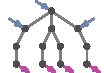
\includegraphics{switchplacement/figures/graph_structure-tree.pdf}%
}
& \screentextcolor{GENERATOR}{$\infty$}
& \screentextcolor{CONSUMER}{$\infty$}
& \screentextcolor{SUSCEPTANCE}{--}
& \screentextcolor{CAPACITY}{--}
& polynomial-time solvable
& 
\cref{ch:network-analyzes:sec:mathematical-model:lem:pf-matrix-is-tum}, 
\cref{ch:facts:thm:fvs},
\cref{ch:foundations:sec:graph-theoretical-flows} p.\ 
\pageref{ch:foundations:sec:graph-theoretical-flows:para:maximum-flow-problem}
& \gls{mf} & \screentextcolor{SUSCEPTANCE}{$\infty$} &
\screentextcolor{CAPACITY}{$\infty$}
\\\addlinespace\addlinespace
% 
2\label{ch:switching:sec:exploit_structural_characteristics:tbl:penrose_minor}
& \gls{mtsfp} and~\gls{otsp}
& penrose-minor-free graphs
& \raisebox{-0.5cm}[0pt][0pt]{
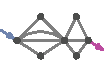
\includegraphics{switchplacement/figures/graph_structure-penrose_minor_free_graph.pdf}}
& \screentextcolor{GENERATOR}{1}
& \screentextcolor{CONSUMER}{1}
& \screentextcolor{SUSCEPTANCE}{--}
& \screentextcolor{CAPACITY}{--}
& polynomial-time solvable
& \cref{ch:switching:sec:exploit_structural_characteristics,ch:switching:sec:computing_one_dtp}
& \gls{dtp}
& \screentextcolor{SUSCEPTANCE}{$\infty$}
& \screentextcolor{CAPACITY}{$\infty$}
\\\addlinespace\addlinespace
% 
\rowcolor{Table-Line-Marker}
%-------------------------------------------------------------------------------
& \gls{mtsfp}
& series-parallel
& % --
& % --
& % --
& \screentextcolor{SUSCEPTANCE}{$\infty$}
& \screentextcolor{CAPACITY}{$\infty$}
& % --
& \parencite{Koc16}
& % --
& % --
& % --
\\
% 
\rowcolor{Table-Line-Marker}
%-------------------------------------------------------------------------------
\multirow{-2}*{3}
\label{ch:switching:sec:exploit_structural_characteristics:tbl:series_parallel}
& and~\gls{otsp}% \acrshort{mtsf} and~\acrshort{ots}
& graphs % series-parallel graphs
& \multirow{-2}*{\raisebox{-0.5cm}[0pt][0pt]{%{-\totalheight}
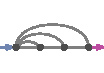
\includegraphics{switchplacement/figures/graph_structure-series_parallel_graph.pdf}}}
& \multirow{-2}*{\screentextcolor{GENERATOR}{1}}
& \multirow{-2}*{\screentextcolor{CONSUMER}{1}}
& \cellcolor{KITpalegreen15}\screentextcolor{SUSCEPTANCE}{$\infty$}
& \cellcolor{KITpalegreen15}\screentextcolor{CAPACITY}{$1$}
& \multirow{-2}*{\NP-hard}
& \cellcolor{KITpalegreen15}\cref{ch:switching:sec:complexity}
& \multirow{-2}*{--}
& \multirow{-2}*{\screentextcolor{SUSCEPTANCE}{--}} 
& \multirow{-2}*{\screentextcolor{CAPACITY}{--}}
\\\addlinespace\addlinespace
% 
4\label{ch:switching:sec:exploit_structural_characteristics:tbl:cactus}
& \gls{mtsfp} and~\gls{otsp}
& cacti with maximum degree of~$3$
& \raisebox{-0.5cm}[0pt][0pt]{%{-\totalheight}
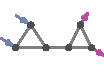
\includegraphics{switchplacement/figures/graph_structure-cacti_graph.pdf}}
& \screentextcolor{GENERATOR}{$\infty$}
& \screentextcolor{CONSUMER}{$\infty$}
& \screentextcolor{SUSCEPTANCE}{1}
& \screentextcolor{CAPACITY}{$\infty$}
& \NP-hard
& \parencite{Leh14}
& \gls{maxst} (see~\cref{ch:switching:sec:approximation_algorithm_on_cacti})
& \screentextcolor{SUSCEPTANCE}{--}
& \screentextcolor{CAPACITY}{--}
\\\addlinespace\addlinespace
% 
\rowcolor{Table-Line-Marker}
%-------------------------------------------------------------------------------
5\label{ch:switching:sec:exploit_structural_characteristics:tbl:2_level_tree}
& \gls{mtsfp} and~\gls{otsp}
& 2-level trees
& \raisebox{-0.5cm}[0pt][0pt]{%{-\totalheight}
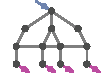
\includegraphics{switchplacement/figures/graph_structure-two_level_tree.pdf}}
& \screentextcolor{GENERATOR}{1}
& \screentextcolor{CONSUMER}{$\infty$}
& \screentextcolor{SUSCEPTANCE}{$\infty$}
& \screentextcolor{CAPACITY}{$\infty$}
& \NP-hard
& \parencite{Leh14}
& --
& \screentextcolor{SUSCEPTANCE}{--}
& \screentextcolor{CAPACITY}{--}
\\\addlinespace\addlinespace
% 
6\label{ch:switching:sec:exploit_structural_characteristics:tbl:plane_graph}
& \gls{mtsfp} and~\gls{otsp}
& planar graph with~$\max$ degree of~$3$
& \raisebox{-0.5cm}[0pt][0pt]{%{-\totalheight}
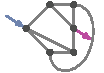
\includegraphics{switchplacement/figures/graph_structure-plane_graph.pdf}}
& \screentextcolor{GENERATOR}{1}
& \screentextcolor{CONSUMER}{1}
& \screentextcolor{SUSCEPTANCE}{$\infty$}
& \screentextcolor{CAPACITY}{1}
& strongly~\NP-hard
& \parencite{Leh14}
& --
& \screentextcolor{SUSCEPTANCE}{--}
& \screentextcolor{CAPACITY}{--}
\\\addlinespace\addlinespace
% 
\rowcolor{Table-Line-Marker}
%-------------------------------------------------------------------------------
& \gls{mtsfp}
& % --
& % --
& \screentextcolor{GENERATOR}{2}
& \screentextcolor{CONSUMER}{2}
& % --
& % --
& % --
& \parencite{Leh14}
& % --
& % --
& % --
\\
% 
\rowcolor{Table-Line-Marker}
%-------------------------------------------------------------------------------
\multirow{-2}*{7}
\label{ch:switching:sec:exploit_structural_characteristics:tbl:arbitrary_graph}
& \cellcolor{KITpalegreen15}\gls{otsp} 
& \multirow{-2}*{arbitrary graphs}
& \multirow{-2}*{\raisebox{-0.5cm}[0pt][0pt]{%{-\totalheight}
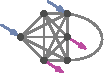
\includegraphics{switchplacement/figures/graph_structure-arbitrary_graph.pdf}}}
& \cellcolor{KITpalegreen15}\screentextcolor{GENERATOR}{1}
& \cellcolor{KITpalegreen15}\screentextcolor{CONSUMER}{$\infty$}
& \multirow{-2}*{\screentextcolor{SUSCEPTANCE}{$\infty$}}
& \multirow{-2}*{\screentextcolor{CAPACITY}{$\infty$}}
& \multirow{-2}*{non-\APX}
& \cellcolor{KITpalegreen15}\parencite{Leh14}
& \multirow{-2}*{--}
& \multirow{-2}*{\screentextcolor{SUSCEPTANCE}{--}} 
& \multirow{-2}*{\screentextcolor{CAPACITY}{--}}
\\\addlinespace\addlinespace
% 
%-------------------------------------------------------------------------------
%-------------------------------------------------------------------------------
   \bottomrule
\end{tabular}

        % 
        \vspace*{-2.0cm}
        % 
        \caption[Overview of results on the complexity of switching.]{Overview
        of known results on the complexity of the~\gls{mtsfp} and~\gls{otsp}.
        The complexity increases from top to bottom as shown in the hardness
        column. Note that the major aspects that influence the complexity of the
        problem are the graph structure of~\glssymbol{graph}, the number of
        \screentextcolor{GENERATOR} {generators~\glssymbol{generators}}, the
        number of
        \screentextcolor{CONSUMER}{consumers~\glssymbol{consumers}}, the
        \screentextcolor{SUSCEPTANCE}{susceptance~\glssymbol{susceptance}}, and the
        \screentextcolor{CAPACITY}{capacity~$\glssymbol{capacity}$}. If there
        are multiple results or if the results differ for~\gls{mtsfp}
        and~\gls{otsp}, we colored the relating entries
        in~\myhl{KITpalegreen15}{green}.}
        % 
        \label{ch:switching:sec:complexity:tbl:complexity-overview}
        % 
    \end{table}
\end{landscape}
% 
%%%%%%%%%%%%%%%%%%%%%%%%%%%%%%%%%%%%%%%%%%%%%%%%%%%%%%%%%%%%%%%%%%%%%%%%%%%%%%%%
\section{Complexity Considerations of using Discrete Control Units}
\label{ch:switching:sec:complexity}
%%%%%%%%%%%%%%%%%%%%%%%%%%%%%%%%%%%%%%%%%%%%%%%%%%%%%%%%%%%%%%%%%%%%%%%%%%%%%%%%
% 
In~\cref{ch:switching:sec:model}, we showed that switching introduces a
quadratic constraint
(see~\cref{ch:switching:sec:model:eq:KVL_quadratic_switching}). Note that models
with quadratic constraints and linear objectives are in
general~\NP-hard~\parencite[278]{Sah74}. The proof uses a reduction from
the~\acrlong{ssp} (\gls{ssp}; see~\textcite[p.245; MP2]{Gar79}
and~\textcite[p.447; MP5]{Aus99} for more information).
% 
However, the quadratic constraint can be replace by a big-M constraint
(see~\cref{ch:switching:sec:model:eq:linearized_switching_geq,ch:switching:sec:model:eq:linearized_switching_leq})
or an indicator constraint
(see~\cref{ch:switching:sec:model:eq:indicator_constraint}). Thus, we lose the
bilinearity and the constraint becomes linear.
% 
%%%%%%%%%%%%%%%%%%%%%%%%%%%%%%%%%%%%%%%%%%%%%%%%%%%%%%%%%%%%%%%%%%%%%%%%%%%%%%%%
\paragraph{Problem Definitions}
\label{ch:switching:sec:problem-definition}
%%%%%%%%%%%%%%%%%%%%%%%%%%%%%%%%%%%%%%%%%%%%%%%%%%%%%%%%%%%%%%%%%%%%%%%%%%%%%%%%
% 
In~\cref{ch:switching:sec:model}, we already defined the optimization
problems~\gls{mtsfp} and~\gls{otsp}. However, in this section we give a finer
granularity of the problem definitions concerning switching to increase the
understanding of the different problems that can be tackled.
% 
The first problem considers switching with a fixed number of preinstalled
switches---meaning~$\gls{switched}\subseteq
\gls{undirectededges}$ is already given---and is
called~$\gls{mtsfp}(\glssymbol{network},\glssymbol{switched})$ and its
value is defined by~$
\opt_{\gls{mtsfp}}(\glssymbol{network},\glssymbol{switched}) \coloneqq
\max_{\{\glssymbol{switch}(\edge)\in\{0,1\}\mid\edge\in
\glssymbol{switched}\}}\allowbreak
\opt_{\gls{mpfp}}(\glssymbol{network}-\bigcup\{\edge\mid\edge\in
\glssymbol{switched}\land\glssymbol{switch}(\edge)=0\})$. The problem is defined
in the following.
% 
\begingroup
    %%%%%%%%%%%%%%%%%%%%%%%%%%%%%%%%%%% Problem %%%%%%%%%%%%%%%%%%%%%%%%%%%%%%%%%%%%
\begin{problem}[framed]{\gls{mtsf}~Problem with Fixed Switches~$\gls{mtsfp}
(\glssymbol{network},\glssymbol{switched})$} 
    % 
    Instance: & A network~\glssymbol{network} and a
    set~$\glssymbol{switched}\subseteq\glssymbol{undirectededges}$.
    \\
    % 
    Objective: & Find a switching~$\glssymbol{switch}(\edge)\in\{0,1\}$ for
    all~$\edge\in\glssymbol{switched}$ such that~$\opt_{\gls{mpfp}}
    (\glssymbol{network}-\{\edge\mid\edge\in
    \glssymbol{switched}\land\glssymbol{switch}(\edge)=0\})$ is maximum among
    all choices of~$\glssymbol{switch}$.
    % 
\end{problem} 
%%%%%%%%%%%%%%%%%%%%%%%%%%%%%%%%%%%%%%%%%%%%%%%%%%%%%%%%%%%%%%%%%%%%%%%%%%%%%%%%
    \label{ch:switching:problems:MTSF_fixed_number_switches-optimization-problem}
\endgroup
% 
The next problem definition will be the first placement problem that relaxes the
definition in the sense that only the number of switches is fixed
by~$k\in\naturals$ with~$\fmagnitude{\glssymbol{switched}} = k$, but the
placement of the switches---meaning the
set~$\glssymbol{switched}\subseteq\glssymbol{undirectededges}$---is unknown.
Thus, we are interested in a maximum possible flow for a
network~\glssymbol{network} and a fixed number of switches~$
\fmagnitude{\glssymbol{switched}} = k$. The problem is called~$\gls{mtsfp}(
\glssymbol{network},k)$ and its value is defined by~$
% 
\opt_{\gls{mtsfp}}(\glssymbol{network},k)
\coloneqq
\max_{
  \glssymbol{switched}\subseteq\glssymbol{undirectededges}
}
\opt_{\gls{mpfp}}(\glssymbol{network}-\glssymbol{switched})
% 
$ with~$\fmagnitude{\glssymbol{switched}} = k$.%
%
\begingroup
    %%%%%%%%%%%%%%%%%%%%%%%%%%%%%%%%%%% Problem %%%%%%%%%%%%%%%%%%%%%%%%%%%%%%%%%%%%
\begin{problem}[framed]{\mtsf~Problem with~$k$-Switches~$\gls{mtsfp}(\glssymbol{network},k)$}
    % 
    Instance: & A network~\glssymbol{network} and a parameter~$k\in\naturals$.
    \\
    % 
    Objective: & Find a set~$\glssymbol{switched}\subseteq
    \glssymbol{undirectededges}$ of switches
    with~$\fmagnitude{\glssymbol{switched}} = k$ such that~$\opt_{\gls{mpfp}}
    (\glssymbol{network}-\glssymbol{switched})$ is maximum among all choices
    of~\glssymbol{switched}.
    % 
\end{problem} 
%%%%%%%%%%%%%%%%%%%%%%%%%%%%%%%%%%%%%%%%%%%%%%%%%%%%%%%%%%%%%%%%%%%%%%%%%%%%%%%%
    \label{ch:switching:problems:MTSF_with_k_switches-Optimization_problem}
\endgroup
% 
Assume that we have no limitation on the number of switches---meaning the number
of switches can be~$\fmagnitude{\glssymbol{switched}} =
\fmagnitude{\glssymbol{undirectededges}}=k$. Thus, the problem to find a maximum
power
flow in network~$\glssymbol{network}$ by allowing as many switches as possible
(\ie, some~$k\in\naturals$) is called~$
% 
  \gls{mtsfp}(\glssymbol{network})
% 
$ with value~$
% 
\opt_{\gls{mtsfp}}(\glssymbol{network})
\coloneqq
\max_{k}\opt_{\gls{mtsfp}}(\glssymbol{network},k)
% 
$.
% 
\begingroup
    %%%%%%%%%%%%%%%%%%%%%%%%%%%%%%%%%%% Problem %%%%%%%%%%%%%%%%%%%%%%%%%%%%%%%%%%%%
\begin{problem}[framed]{\acrlong{mtsfp}~$\gls{mtsfp}(\glssymbol{network})$}%
    Instance: & A network~\glssymbol{network}.\\
    % 
    Objective: & Find a
    set~$\glssymbol{switched}\subseteq\glssymbol{undirectededges}$ of switched
    edges such
    that~$\opt_{\gls{mpfp}}(\glssymbol{network}-\glssymbol{switched})$ is maximum
    among all choices of switched edges~\glssymbol{switched}.
\end{problem}%
    \label{ch:switching:problems:MTSF_with_k_switches-Optimization_problem:2}
\endgroup
% 
The latter problem allows as many switches as necessary to obtain a best
possible power flow. However, when there is only one generator and one demand
the maximum number of switches~$\fmagnitude{\glssymbol{switched}}$ is restricted
by~$\fmagnitude{\glssymbol{vertices}}-1$ that represents a tree. Removing more
edges would lead---independent on the generation limits---to an infeasible
solution, since some demands are cut-off from any generator. If we have multiple
generators and demands the maximum number would be restricted by a
forest~$\fmagnitude{\glssymbol{vertices}}-k$, where~$k$ represents the number of
connected components. Note that the number of connected components can be
still~$k=1$.

In general an desirable investigation is the minimum number of
switches---meaning the smallest~$k$---such that we get the same value
as~$\opt_{\gls{mtsfp}}(\glssymbol{network})$. This problem is called~$
% 
\opt_{\gls{mnsp}}(\glssymbol{network})
\coloneqq
\min_{
  \opt_{\gls{mtsfp}}(\glssymbol{network},k)
  =
  \opt_{\gls{mtsfp}
}(\network)} k
% 
$ with the value~$\opt_{\gls{mtsfp}}(\glssymbol{network})$. 
% 
\begingroup
    %%%%%%%%%%%%%%%%%%%%%%%%%%%%%%%%%%% Problem %%%%%%%%%%%%%%%%%%%%%%%%%%%%%%%%%%%%
\begin{problem}[framed]{\acrlong{mnsp}
    under~\gls{mtsf}~$\gls{mnsp}(\glssymbol{network},k)$} 
    % 
    Instance: & A network~\glssymbol{network} and~$k\in\naturals$.\\
    % 
    Question: & Is it possible to remove a set of edges~$
    \glssymbol{switched}\subseteq\glssymbol{edges}$
    such that $k = \fmagnitude{\glssymbol{switched}}$ is minimum among all
    choices of~$\opt_{\gls{mtsfp}}(\glssymbol{network})$?
    % 
\end{problem} 
%%%%%%%%%%%%%%%%%%%%%%%%%%%%%%%%%%%%%%%%%%%%%%%%%%%%%%%%%%%%%%%%%%%%%%%%%%%%%%%%
    \label{ch:switching:problems:MNS_under_MTSF-Optimization_problem}
\endgroup
% 
Note that similar definitions can be made for the~\gls{otsp}. An overview of the
switching related problems is given
in~\cref{app:problems:discrete-placement-problems}.
% 
\paragraph{Decision Problems}
% 
\gls{mtsfp} is an optimization problem that involves searching for the best
solution from some large set of solutions. Any optimization problem can be
transformed into a decision problem by asking whether the optimum value is at
least or at most~$k$ for some~$k\in\reals$. We denote the corresponding decision
problem for~$\gls{mtsfp}(\glssymbol{network})$ by~\kmtsfp.
%
\begingroup
    %%%%%%%%%%%%%%%%%%%%%%%%%%%%%%%%%%% Problem %%%%%%%%%%%%%%%%%%%%%%%%%%%%%%%%%%%%
\begin{problem}[framed]{\kMTSFP~\kmtsfp$(\glssymbol{network},k)$} 
    Instance: & A network~\glssymbol{network} and
    $k\in\posrationals$.\\
    % 
    Question: & Is it possible to remove a set of edges~\glssymbol{switched} such
    that there is an electrically feasible flow~\glssymbol{flow} in
    $\glssymbol{network}-\glssymbol{switched}$ with flow
    value~$\glssymbol{flowvalue}( \glssymbol{network} - 
    \glssymbol{switched}, \glssymbol{flow}) \geq k$?%
    % 
\end{problem} 
%%%%%%%%%%%%%%%%%%%%%%%%%%%%%%%%%%%%%%%%%%%%%%%%%%%%%%%%%%%%%%%%%%%%%%%%%%%%%%%%
    \label{ch:switching:problems:MNS_under_MTSF-Decision_Problem}
\endgroup
% 
Note that decision problems are often used to show that a particular problem
is~\NP-hard. We will use this problem
in~\cref{ch:switching:sec:complexity:subsec:np_hardness_Source_Sink_MTSF_capacity1}
to show that~$\gls{mtsfp}(\glssymbol{network})$ is~\NP-hard. An overview of the
switching decision problems can be found
in~\cref{app:problems:discrete-placement-problems}.
% 
%%%%%%%%%%%%%%%%%%%%%%%%%%%%%%%%%%%%%%%%%%%%%%%%%%%%%%%%%%%%%%%%%%%%%%%%%%%%%%%%
\subsection{Literature Overview}
\label{ch:switching:sec:complexity:subsec:overview}
%%%%%%%%%%%%%%%%%%%%%%%%%%%%%%%%%%%%%%%%%%%%%%%%%%%%%%%%%%%%%%%%%%%%%%%%%%%%%%%%
% 
We will see
in~\cref{ch:switching:sec:exploit_structural_characteristics:def:penrose-graph}
(see
also~\cref{ch:switching:sec:exploit_structural_characteristics:subsec:dtp_analyses,ch:switching:sec:exploit_structural_characteristics:fig:forbidden_minor})
that for single-source single-sink penrose-minor-free graphs
(see~\cref{ch:switching:sec:complexity:tbl:complexity-overview}--\screen{1})
the~$\gls{mtsfp}(\glssymbol{network})$ is poly\-no\-mi\-al-time solvable. We
will look at this structure
in~\cref{ch:switching:sec:exploit_structural_characteristics:subsec:dtp}.
However, \textcite{Koc16} showed that for arbitrary
susceptance~\glssymbol{susceptance} and capacity~$\glssymbol{capacity}$ this
problem is already~\NP-hard\footnote{We found out about that proof after the
publication of the later proof in~
\parencite{Gra18} thanks to Thomas William Brown.}.
In~\cref{ch:switching:sec:complexity:subsec:np_hardness_Source_Sink_MTSF_capacity1},
we will provide a different reduction that is also a generalization of the proof
of~\textcite{Koc16}. Contrary to series-parallel graphs, cactus graphs have the
special property that the cycles in a cactus do not share an edge. Thus, the
dependencies on the voltage angles of a vertex decrease. Though, for
single-source single-sink this problem is polynomial-time solvable, it becomes
already~\NP-hard for an arbitrary number of generators and consumers
(see~\cref{ch:switching:sec:complexity:tbl:complexity-overview}--\screen{3}).
\textcite[pp.8ff.; Section 5]{Leh14} motivated another non-standard graph
structure from the disaster management. The idea is that after a blackout
a~\gls{tso} will try to recover the power grid by establishing a tree-like
structure. The graph structure is denoted by N-level tree
(see~\cref{ch:switching:sec:complexity:tbl:complexity-overview}--\screen{4}),
which has a generator at the root and consumers at the leaves. For each level
there is a total order of the vertices that also defines the intra-level
neighbors of a vertex. The tree allows intra-level connections to direct
neighbors. Note that these intra-level connections cause cycles that share edges
with other cycles. Thus, this structure is more complex than a cactus. The next
graph structure that is more complex are planar graphs (see~
\cref{ch:switching:sec:complexity:tbl:complexity-overview}--\screen{5}) for
which \textcite[p.13; Section 7]{Leh14} show that the problem is strongly
\NP-hard for planar graphs with maximum degree of 3, one generator, one
consumer, and having unit capacities. Naturally this problems stays \NP-hard for
arbitrary graphs, but it is not possible for any~$\epsilon > 0$ to find an
approximation algorithm within a factor of~$2^{\bigO((\log n)^
{1-\epsilon})}$~\parencite[pp.10ff.]{Leh14}~\parencite[pp.95ff.]{Karger1997}.
% 
%%%%%%%%%%%%%%%%%%%%%%%%%%%%%%%%%%%%%%%%%%%%%%%%%%%%%%%%%%%%%%%%%%%%%%%%%%%%%%%
\subsection{NP-hardness of Source-Sink-MTSF on Series-Parallel-Graphs}
\label{ch:switching:sec:complexity:subsec:np_hardness_Source_Sink_MTSF_capacity1}
%%%%%%%%%%%%%%%%%%%%%%%%%%%%%%%%%%%%%%%%%%%%%%%%%%%%%%%%%%%%%%%%%%%%%%%%%%%%%%% 
% 
First we prove that~\gls{mtsfp} is in~\NP\ by providing a polynomial time
algorithm that is denoted by~$\mathtt{valid}(\glssymbol{network},
\glssymbol{switched})$. The polynomial algorithm specifies whether the set of
switched edges~\glssymbol{switched} is a valid solution for an
instance~\glssymbol{network}. It is not hard to determine that an
instance~\glssymbol{network} and a solution~\glssymbol{switched} are properly
defined (\cref{ch:switching:sec:model}). Checking whether a
switching~\glssymbol{switched} provides an electrically feasible flow that is at
least~$k$ can be done by~\acrlong{lp} (\gls{lp}) in polynomial time
(see~\cref{ch:switching:sec:model}).

To show that~\kmtsfp\ is also~\NP-hard we reduce the~\acrlong{ssp} to~\kmtsfp.
% 
%%%%%%%%%%%%%%%%%%%%%%%%%%%%%%%%%%%% FIGURE %%%%%%%%%%%%%%%%%%%%%%%%%%%%%%%%%%%
\begin{figure}[tb!]
    \centering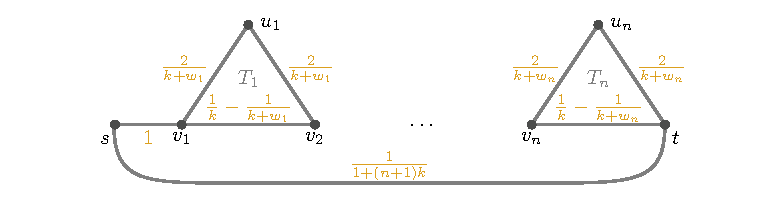
\includegraphics[page=1]
    {switchplacement/figures/hardness_proof.pdf}
    %
    \vspace*{1.3mm}
    \caption[A network constructed from~\gls{ssp}.]{A
    network~\glssymbol{network} constructed from an instance of~\gls{ssp}
    having one source~$\source\in\glssymbol{generators}$ (\ie, $
    \fmagnitude{\glssymbol{generators}}\equiv 1$) and one
    sink~$\sink\in\glssymbol{consumers}$ (\ie, $
    \fmagnitude{\glssymbol{consumers}}\equiv 1$).
    All edges $ (\vertexa,\vertexb)\in\glssymbol{edges}$ have
    a~\screentextcolor{CAPACITY}{capacity}
    of~\screentextcolor{CAPACITY}{$\glssymbol{capacity}\equiv1$} and the
    \screentextcolor{SUSCEPTANCE}{susceptances~\glssymbol{susceptance}}
    are shown next to the edges.}
    %
    \label{ch:switching:sec:complexity:fig:reduction}
\end{figure}
%
%
\begingroup
    \begin{problem}[framed]{\acrlong{ssp}~$\gls{ssp}(W,k)$}
    Instance: & A finite set of numbers~$W=\{w_1,w_2,\dots,w_n\}$
    with~$w_i\in\naturals$ and a~$k\in\naturals$.\\ %
    Question: & Is there a set of elements~$x_1,\dots,x_n\in\{0,1\}$ such that 
    %
    $\sum_{j=1}^{n}w_jx_j = k$?
\end{problem}
    \label{ch:switching:problems:subset-sum-decision-problem}
\endgroup
%
\begin{lemma}
    \kmtsfp\ is~\NP-complete even if there is only one source and one sink in
    the network and all edge capacities are~$1$.
\end{lemma}
% 
\begin{proof}
  We show the~\NP-hardness by reducing~\gls{ssp} to this
  restricted~\gls{mtsfp}-variant in polynomial time. Since~\gls{ssp} is
  % 
  weakly~\NP-complete~\parencite{Gar79}, \gls{mtsfp} is~\NP-hard, too.
 %
 Given an~\gls{ssp}-instance~$(W, k)$ we construct an instance
 of~\gls{mtsfp} that allows a flow of~$2$ if and only if there is a solution
 of the~\gls{ssp}-instance. We may assume without loss of generality that
 no element of~$W$ is larger than~$k$ as these elements are never part of any
 solution. In the constructed network~\glssymbol{network} there is one
 source~$\{\source\}\eqqcolon\glssymbol{generators}$ (\ie, $
 \fmagnitude{\glssymbol{generators}}\equiv 1$) and one sink~$
 \{\sink\}\eqcolon\glssymbol{consumers}$ (\ie, $
 \fmagnitude{\glssymbol{consumers}}\equiv 1$;
 see~\cref{ch:switching:sec:complexity:fig:reduction}). All
 edges~$\edge\in\glssymbol{edges}$ have
 capacity~$\glssymbol{capacity} \equiv 1$. There is one edge from~\source to~\sink
 with susceptance~$\nicefrac{1}{(1+(n+1)k)}$, where~$n=\fmagnitude{W}$. For each
 element~$w_i\in W$ we build a triangle with vertices~$\vertex_i$, $\vertexa_i$,
 and~$\vertex_ {i+1}$. We
 set~$\glssymbol{susceptance}(\vertex_i,\vertexa_i)\coloneqq
 \glssymbol{susceptance}
 (\vertexa_i,\vertex_{i+1})\coloneqq\nicefrac{2}{(k+w_i)}$
 and~$\glssymbol{susceptance}(\vertex_i,\vertex_{i+1})\coloneq\nicefrac{1}{k} -
 \nicefrac{1}{(k+w_i)}$. Note that the triangles for~$w_i$ and~$w_{i+1}$ have
 the vertex~$\vertex_{i+1}$ in common. We set~$v_{n+1}=t$ and add the
 edge~$(\source,\vertex_1)$ with
 susceptance~$\glssymbol{susceptance}(\source,\vertex_1) = 1$. Note that the
 edge~$(\source,\vertex_1)$ is necessary when we do not switch any triangle,
 since this would exceed the flow of one in the upper part.
 
 To achieve a flow of~$2$ in the network both edges incident to~\source must be
 saturated. In particular, the flow through the chain of triangles is~$1$
 and~$\glssymbol{voltageangledifference}(\source,\sink)=1+(n+1)k$. Consider the
 triangle~$T_i$ for the element~$w_i\in W$. In this triangle~$v_i$ acts as a
 source and~$\vertex_{i+1}$ as a sink. There are two paths from~$\vertex_i$
 to~$\vertex_{i+1}$ in~$T_i$: The direct path consisting only of the
 edge~$(\vertex_i,\vertex_{i+1})$ and the path via~$u_i$. In any solution
 to~\glssymbol{network} at most one of these paths may be switched as otherwise
 the total flow in~\glssymbol{network} is at most~$1$. If no edge in~$T_i$ is
 switched
 (\cref{ch:switching:sec:complexity:fig:switching_triangles_hardness}\screen{a}),
 we obtain~$\glssymbol{voltageangledifference}(\vertex_i,\vertex_{i+1})\equiv k$
 for one unit flowing through~$T_i$. If the edge~$(\vertex_i,\vertex_{i+1})$ is
 switched
 (\cref{ch:switching:sec:complexity:fig:switching_triangles_hardness}\screen{b}),
 we have~$\glssymbol{voltageangledifference}( \vertex_i, \vertex_{i+1} ) = k +
 w_i$. If an edge incident to~$\vertexa_i$ is switched
 (\cref{ch:switching:sec:complexity:fig:switching_triangles_hardness}\screen{c}),
 the flow on~$(\vertex_i,\vertex_{i+1})$ must be equal to~$1$ and we get
% 
%%%%%%%%%%%%%%%%%%%%%%%%%%%%%%%%%%%% FIGURE %%%%%%%%%%%%%%%%%%%%%%%%%%%%%%%%%%%
\begin{figure}[tb!]
    \centering
    % 
    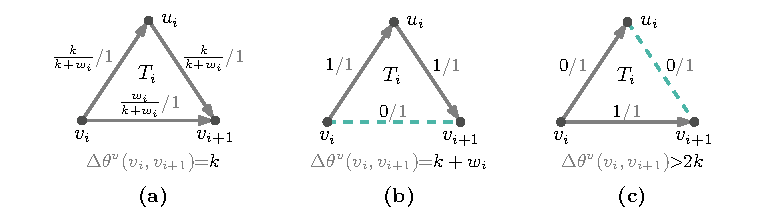
\includegraphics[page=1,trim={0 0.5mm 0 0}, clip]
    {switchplacement/figures/switching_triangles_in_hardness_proof.pdf}
    % 
    \caption[Possible ways to switch in a triangle in a network constructed
    from~\gls{ssp}]{ Possible ways to switch the triangles~$T_i$ in a
    network~\glssymbol{network} with corresponding angle differences and flows.
    (a)~If no edges are switched the angle difference is~$k$. (b)~If the
    edge~$(v_i,v_{i+1})$ is \screentextcolor{KITgreen70}{switched}, the angle
    difference is~$k+w_i$. (c)~If an edge incident to~$u_i$ is
    \screentextcolor{KITgreen70}{switched},
    the angle difference is larger than~$2k$. }
    % 
    \label{ch:switching:sec:complexity:fig:switching_triangles_hardness}
\end{figure}
 % 
 \begin{align*}
  \glssymbol{voltageangledifference}(\vertex_i,\vertex_{i+1})
   = \frac{1}{\frac{1}{k} - \frac{1}{k+w_i}}
   = \frac{k(k+w_i)}{w_i}
   = \frac{k^2}{w_i} + k
   > 2k.
 \end{align*}
 % 
 Note that in any
 case~$\glssymbol{voltageangledifference}(\vertexb_i,\vertexb_{i+1})\geq k$. If
 in any triangle~$T_i$ an edge incident to~$\vertexa_i$ is switched, we have
 % 
 \begin{align*}
  \glssymbol{voltageangledifference}(\source,\sink)
  &= \glssymbol{voltageangledifference}(\source,v_1) + \sum_{i=1}^n 
  \glssymbol{voltageangledifference}(\vertex_i,\vertex_{i+1}) \\
  &> 1 + (n-1)k + 2k
  = 1+ (n+1)k,
 \end{align*}
 % 
 which contradicts~$\glssymbol{voltageangledifference}(\source,\sink)=1+(n+1)k$.
 Hence, only the edges~$(\vertex_i,\vertex_{i+1})$ for~$i=1,\dots,n$ may be
 switched.
 
 If there is a set~\glssymbol{switched} of edges in~\glssymbol{network} such
 that removing them from the network yields a maximum flow~\glssymbol{flow}
 in~$\glssymbol{network}-\glssymbol{switched}$ with
 throughput~$\glssymbol{flowvalue}(\network, \glssymbol{flow}) \equiv 2$, we can
 construct a solution to the corresponding~\gls{ssp}-instance as follows.
 Let~$x_i = 1$ if~$(v_i,v_{i+1})\in
 \glssymbol{switched}$ and~$x_i=0$ otherwise. By the argumentation above we
 have~$\glssymbol{voltageangledifference}(\vertex_i,\vertexb_{i+1}) = k + w_i$
 if~$x_i = 1$ and~$\glssymbol{voltageangledifference}
 (\vertexb_i,\vertexb_{i+1})=k$ otherwise. Hence, we have
 % 
 \begin{align*}
 1+(n+1)k
 &=\glssymbol{voltageangledifference}(\source,\sink)\\
 &= \glssymbol{voltageangledifference}(\source,v_1) 
 + 
 \sum_{i=1}^n\glssymbol{voltageangledifference}(v_i,v_{i+1})\\
 &= 1 + \sum_{i=1}^n(k+x_i w_i)\\
 &= 1 + nk +\sum_{i=1}^n x_i w_i.
 \end{align*}
 % 
 and therefore~$\sum_{i=1}^n x_i w_i = k$ as required by
 the~\gls{ssp}-instance.
 
 If the~\gls{ssp}-instance has a solution, \ie, $\sum_{i=1}^n x_i w_i = k$
 for a suitable assignment of the~$x_i$, we define~$\glssymbol{switched} \coloneqq
 \{
 (\vertexb_i,\vertexb_{i+1}) \mid x_i=1\}$. We claim that after switching these
 edges the remaining network~$\glssymbol{network}-\glssymbol{switched}$ admits a
 power flow with value~$2$. Setting~$\glssymbol{voltageangle}(\source)=0$
 and~$\glssymbol{voltageangle}(\vertexb_i) = 1 + \sum_{j=1}^{i-1}(k + x_i w_i)$
 induces a feasible electrical flow of~$1$ on the triangle chain by the
 arguments above. We further note that
 % 
 \begin{align*}
 \glssymbol{voltageangledifference}(\source,\sink)
 &= \glssymbol{voltageangledifference}(\source,\vertexb_1) + \sum_{i=1}^n\glssymbol{voltageangledifference}(\vertexb_i,\vertexb_{i+1})\\
 &= 1 + \sum_{i=1}^n(k+x_iw_i)\\
 &= 1 + nk + \sum_{i=1}^n x_i w_i\\
 &= 1 + (n+1)k.
 \end{align*}
 % 
 Hence, we have~$\glssymbol{flow}(\source,\sink)\equiv 1$ and the total flow
 in~$\glssymbol{network}-\glssymbol{switched}$ is~$2$.
 
 The size of the constructed network is linear in~$\fmagnitude{W}$ and all
 parameters are polynomial in~$k$. Hence, the reduction from~\gls{ssp}
 to~\gls{mtsfp} runs in polynomial time. Since~\gls{ssp}
 is~\NP-complete~\parencite{Gar79}, this reduction implies that~\gls{mtsfp}
 is~\NP-hard even if we restrict ourselves to networks with unit capacities and
 only one source and one sink.
\end{proof}
% 
%
%%%%%%%%%%%%%%%%%%%%%%%%%%%%%%%%%%%%%%%%%%%%%%%%%%%%%%%%%%%%%%%%%%%%%%%%%%%%%%%
\section{Network Modeling}\label{ch:switching:sec:network_modeling}
%%%%%%%%%%%%%%%%%%%%%%%%%%%%%%%%%%%%%%%%%%%%%%%%%%%%%%%%%%%%%%%%%%%%%%%%%%%%%%%
%
The model presented in~\cref{ch:switching:sec:model} places no restriction on
the network. Our algorithms and proofs are often simpler if the underlying
network has a specific form.
% 
%%%%%%%%%%%%%%%%%%%%%%%%%%%%%%%%%%%% FIGURE %%%%%%%%%%%%%%%%%%%%%%%%%%%%%%%%%%%%
\begin{figure}[t!]%
% 
\centering
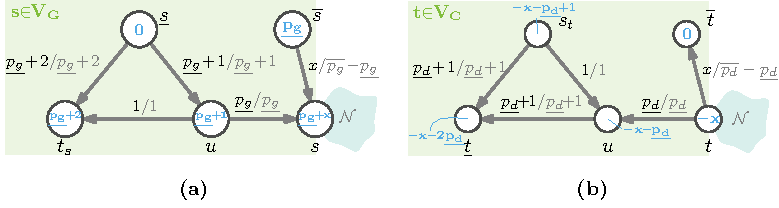
\includegraphics{switchplacement/figures/bounded_unbounded_mtsf_transformation.pdf}%
%
\caption[The transformation of an unbounded into a bounded network.]{
  A bounded network can be transformed to an unbounded network by
  adding substructures to its generator and consumer vertices. (a)~A
  \myhl{KITpalegreen15}{generator~$\source\in\glssymbol{generators}$} in a
  bounded~\gls{mtsfp} can be transformed to a generator in an
  unbounded~\gls{mtsfp} by modifying
  the~\myhl{KITcyanblue15}{network~$\glssymbol{network}$} at the source.
  Thereby, a generator with non-zero lower bound generation can be replaced by a
  construction of a cycle with generator~$\underline{\source}$ and
  consumer~$\sink_{\source}$ forcing a generation
  of~\glssymbol{realpowergenerationmin} on edge~$(\vertexa,\source)$, and a
  generator~$\overline{\source}$ allowing a generation in total of up
  to~\glssymbol{realpowergenerationmax} at vertex~\source.
  (b)~For~\myhl{KITpalegreen15}{consumers~\sink} to model the upper bound it
  suffices to add an edge~$(\overline{\sink},\sink)$ and a minimum demand
  of~\glssymbol{realpowerdemandmin} to~$\overline{\sink}$. To model the lower
  bound, a triangle that configures the voltage angles in such a fashion that
  there is a feasible power flow only if at least the lower demand is satisfied.
  % 
  }
  % 
\label{ch:switching:sec:network_modeling:fig:bounded_unbounded_mtsf_transformation}%
\end{figure}%
%%%%%%%%%%%%%%%%%%%%%%%%%%%%%%%%%%%%%%%%%%%%%%%%%%%%%%%%%%%%%%%%%%%%%%%%%%%%%%%%

Without loss of generality we may assume that in the network
$\glssymbol{network} \coloneqq$ (\glssymbol{graph},
\glssymbol{generators},\glssymbol{consumers}, $\glssymbol{capacity}$,
\glssymbol{susceptance},
\realpowerdemandmin) all generators and consumers are degree\nobreakdash-1
vertices. We achieve this by adding an edge with infinite capacity and a
susceptance of~$1$ between each generator or
consumer~$\vertexb\in(\glssymbol{generators}\cup\glssymbol{consumers})$ and a new
vertex~$\vertexa_{\vertexb}$. The new vertex~$\vertexa_{\vertexb}$ then acts as a
generator or consumer and~\vertexb becomes an intermediate vertex. We use this
assumption especially
in~\cref{ch:switching:sec:exploit_structural_characteristics}, where we restrict
our network to certain graph classes.

We can shrink the network~\glssymbol{network} by contracting degree-2 vertices.
For this we introduce the \emph{susceptance norm} of a path
$\fpath{}{\vertexa}{\vertexb}$, which is defined as
%
\begin{equation}%
    \bnorm{\fpath{}{\vertexa}{\vertexb}}
    \coloneqq
    \sum_{\edge\in\fpath{}{\vertexa}{\vertexb}}
    \glssymbol{susceptance}(\edge)^{-1},
    % 
    \label{eq:bnorm}%
\end{equation}%
% 
and gives us a distance metric on power grids. 
% 
The susceptance norm is a norm, since it fulfills the axioms given
by~\textcite{Ban22}.
% 
\begin{enumerate}
    \item $\norm{\vv{x}}{}\hspace{7.2mm}\equiv 0$ if and only if $\vv{x}\equiv
    \vv{0}$
    (neutral element),
    \item $\norm{ s \cdot \vv{x} }{}\hspace{3mm}\equiv \fmagnitude{s}\cdot\norm{\vv{x}}{}$ 
    \hspace*{21.5mm}(absolute homogeneity),
    \item $\norm{\vv{x}+\vv{y}}{}\leq\norm{\vv{x}}{} + \norm{\vv{y}}{}$ 
    \hspace*{16.5mm}(triangular inequality).
\end{enumerate}
% 
Applying the following lemma we
can simplify~\glssymbol{network} by contracting paths to single edges.
%
%%%%%%%%%%%%%%%%%%%%%%%%%%%%%%%%%% LEMMA %%%%%%%%%%%%%%%%%%%%%%%%%%%%%%%%%
\begin{lemma}%
  A simple path~$\pathu$ in~\glssymbol{network} whose internal vertices have
  degree 2 in~\glssymbol{network} and are neither generators nor consumers is
  equivalent to a single edge~\edge with capacity~$\glssymbol{capacity}
  (\edge)\coloneqq\min_{(\vertexa,\vertexb)\in\pathu}\glssymbol{capacity}
  (\vertexa,\vertexb)$
  and susceptance~$\glssymbol{susceptance}(\edge)\coloneqq\nicefrac{1}{
\bnorm{\pathu}}$.%
\label{ch:switching:sec:network_modeling:lem:series_contraction}
\end{lemma}%
%
Note that if we assume that all generator and consumer vertices have degree 1,
they are never internal vertices of any simple path. Note
that~\cref{ch:switching:sec:network_modeling:lem:series_contraction} is
equivalent to the
transformation~\cref{ch:network-analyzes:sec:mathematical-model:sim:series_contraction}
presented in~\cref{ch:network-analyzes:sec:reduction-transformation-rules}.

\textcite{Leh14,Leh15a} showed that the bounded~\gls{mtsfp} is~\NP-hard on
cacti (\ie, a graph consisting of edge disjoint cycles). We can transform a
bounded~\gls{mtsfp} with network~\dcnetworktuple to an
unbounded~\gls{mtsfp}. We model the upper bounds by adding
edges~$(\vertexa,\vertexb)$ with appropriate capacities at
vertices~$\vertexa\in(\glssymbol{generators}\cup\glssymbol{consumers})$. To
model a
% 
non-zero lower generation bound~$\glssymbol{realpowergenerationmin}$ at a
generator, we replace it by the construction shown
in~\cref{ch:switching:sec:network_modeling:fig:bounded_unbounded_mtsf_transformation}\screen{a},
which is based on a structure used by~\textcite{Leh14}. The cycle with
generator~$\underline{\source}$ and consumer~$\sink_{\source}$
with~$\glssymbol{realpowerdemandmin}(\sink_\source) =
\glssymbol{realpowergenerationmin} + 2$ forces a flow
of~$\glssymbol{realpowergenerationmin}$ on the edge~$(\vertexa,\source)$ and the
generator~$\overline{\source}$ is able to add the remaining generation capacity.
Note that the cycle can be omitted if~$\glssymbol{realpowergenerationmin} \equiv
0$. For consumers we just add an edge~$(\overline{\sink},\sink)$ with a capacity
of~\glssymbol{realpowerdemandmax} to model the upper bound. In addition, the
minimum demand is modeled by a triangle for which the voltage angle
configuration enforces a minimum demand of~\glssymbol{realpowerdemandmin}
(\cref{ch:switching:sec:network_modeling:fig:bounded_unbounded_mtsf_transformation}\screen{b}).
%
\begin{lemma}%
  Every bounded~\gls{mtsfp} can be transformed into an
  unbounded~\gls{mtsfp} on a network with size linear
  in~$\fmagnitude{\glssymbol{vertices}}$ and~$\fmagnitude{\glssymbol{edges}}$.
  % 
  \label{lem:bounded_unbounded_mtsf_transformation}%
\end{lemma}%
%%%%%%%%%%%%%%%%%%%%%%%%%%%%%%%%%%%% FIGURE %%%%%%%%%%%%%%%%%%%%%%%%%%%%%%%%%%%%
\begin{figure}[t!]%
  \centering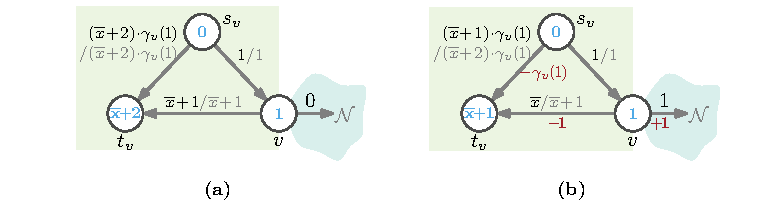
\includegraphics{switchplacement/figures/ots_mtsf_transformation.pdf}
  %
  \caption[Transformation from an~\gls{otsp}- to an~\gls{mtsfp}-instance.]{
    Transforming an~\gls{otsp}-instance to an~\gls{mtsfp}-instance is
    possible by adding triangles at consumer vertices. The
    edge~$\edge=(\source_\vertex,\sink_\vertex)$ and the other two edges have
    susceptances~$\glssymbol{susceptance}(\edge)=\cost_\vertex(1)$ and~$1$,
    respectively. (a)~The maximum flow in a triangle is obtained by injecting no
    power to the network~\glssymbol{network} from~\vertex. (b)~Per injected unit
    of flow from~\vertex to~\glssymbol{network}, there is a decrease in flow
    value by~$\cost_\vertex(1)$ (\textcolor{KITred}{red}) in a triangle.}
  % 
  \label{fig:ots_mtsf_transformation}%
\end{figure}%
%
%
\textcite[Lemma 2]{Leh14} show that
every~\gls{mtsfp}-instance can be transformed to an equivalent
\gls{otsp}-instance while maintaining the network structure. The idea is
basically that we pay for each unit a consumer is not used to its maximum
capacity~\glssymbol{realpowerdemandmax}
meaning~$\glssymbol{realpowerdemandmax}(\vertexa)-\glssymbol{netflow}
(\vertexa)\neq 0$ and we
pay~$\fmagnitude{\glssymbol{realpowerdemandmax}(\vertexa)-\glssymbol{netflow}
(\vertexa)}$ units. This transformation is done by defining a generator cost
function~$\gamma\colon\glssymbol{generators}\cup\glssymbol{generators}'\to\posreals$
with~$\vertexa\in\glssymbol{generators}'$ if~$\vertexa\in\glssymbol{consumers}$
and~$\gamma_\vertexa (1)\equiv 1$ with~$\vertexa\in\glssymbol{generators}'$
and~$\gamma_\vertexa(1)\equiv 0$ for all~$\vertexa\in\glssymbol{generators}$. In
addition, the consumptions are fixed
meaning~$\glssymbol{realpowerdemandmin}(\vertexa) =
\glssymbol{realpowerdemandmax}(\vertexa) =
\glssymbol{realpowerdemand}(\vertexa)$ for all~$\vertexa\in\glssymbol{consumers}$. Thus, while
maximizing the power flow a generator~$\vertexa\in\glssymbol{generators}'$
produces~$\glssymbol{realpowerdemandmax}(\vertexa)-\glssymbol{netflow}(\vertexa)$ units of
flow.

We present the reverse transformation for
\gls{otsp} with linear cost functions. Let~\dcnetworktuple be a bounded
network, where each consumer~$\vertex\in\glssymbol{consumers}$ has a fixed
demand~$\glssymbol{realpowerdemand}(\vertex) =
\glssymbol{realpowerdemandmin}(\vertex) =
\glssymbol{realpowerdemandmax}(\vertex)$. At each
generator~$\vertex\in\glssymbol{generators}$ with cost~$\cost_{\vertex}(1)$ per
generated unit of power we add a triangle consisting of~\vertex, another
generator~$\source_{\vertex}$ and a consumer~$\sink_{\vertex}$ as shown
in~\cref{fig:ots_mtsf_transformation}. The
edge~$(\source_\vertex,\sink_\vertex)$ has susceptance~$\cost_{\vertex}(1)$ and
the other two edges have susceptance~$1$. We denote the resulting network
by~$\glssymbol{network}'$.
%
If~$\vertex$ injects no power into the original network
(\cref{fig:ots_mtsf_transformation}\screen{a}), all its generated power flows
along~$(\vertex, \sink_\vertex)$ to~$\sink_\vertex$. The flow in this triangle
is then maximized by sending $1$ unit from $\source_{\vertex}$ via~\vertex to
$\sink_\vertex$ and $(\maxexcess_\vertex+2)\cdot\cost_{\vertex}(1)$ units
directly on $(\source_\vertex, \sink_\vertex)$. Per unit of flow injected
by~\vertex into the original network, the angle difference
$\glssymbol{voltageangledifference}(\vertex, \sink_{\vertex})$ decreases by~$1$
(\cref{fig:ots_mtsf_transformation}\screen{b}). Therefore,
$\glssymbol{voltageangledifference}(\source_\vertex, \sink_\vertex)$ also
decreases by $1$ and the flow~$\glssymbol{flow}(\source_\vertex,
\sink_{\vertex})$ by~$\cost_\vertex(1)$. Hence, a feasible flow
in~$\glssymbol{network}$ with cost~$k$ can be transformed to a feasible flow
in~$\glssymbol{network}'$ with flow value~$M-k$, where~$
M
=
\sum_{\vertex\in\glssymbol{generators}}
\left((\glssymbol{realpowergenerationmax}(\vertex)+2)\cdot\cost_\vertex(1)
+
\glssymbol{realpowergenerationmax}(\vertex) + 1\right)
% 
$. This leads to the following lemma.
% 
\begin{lemma}
    \label{lem:ots_msf_transformation}
    For every~\gls{otsp}-instance~\dcnetworktuple with fixed
    demands~$\glssymbol{realpowerdemand}(\vertex) =
    \glssymbol{realpowerdemandmin}(\vertex) =
    \glssymbol{realpowerdemandmax}(\vertex)$ and linear cost
    functions~$\cost_{\vertex}$ for each
    consumer~$\vertex\in\glssymbol{consumers}$ there is
    an~\gls{mtsfp}-instance~$\glssymbol{network}'$ and a
    constant~$M\in\posreals$ such that for every~$k\in\posreals$ we
    have~$\opt_{\gls{otsp}}(\glssymbol{network})\le k$ if and only
    if~$\opt_{\gls{mtsfp}}(\glssymbol{network}')\ge M-k$. Moreover, the size
    of~$\glssymbol{network}'$ is linear in the size of~\glssymbol{network}.
% 
\end{lemma}
% 
The previous lemma and the result of~\textcite[Lemma 2]{Leh14} provide a
possibility to interchangeably apply algorithms found for~\gls{mtsfp}
to~\gls{otsp} (and vice versa) by a simple graph transformation.

% 
%%%%%%%%%%%%%%%%%%%%%%%%%%%%%%%%%%%%%%%%%%%%%%%%%%%%%%%%%%%%%%%%%%%%%%%%%%%%%%%
\section{MTSF on Source-Sink-Networks}
\label{ch:switching:sec:exploit_structural_characteristics}
%%%%%%%%%%%%%%%%%%%%%%%%%%%%%%%%%%%%%%%%%%%%%%%%%%%%%%%%%%%%%%%%%%%%%%%%%%%%%%%
%
\textcite{Fis08} found in their experiments that \emph{Wheatstone Bridges}
\parencite{905717} (bridges or short-cut edges in a cycle with four edges) can
be associated with \emph{Braess's Paradox}~\parencite{Bra05,Pal12,Nag10}, in
which adding a line to a network (even with zero cost) can increase the cost of
using that network
(see~\cref{ch:related-work:sec:braess-paradox}).
These structures are often removed by switches in their results. In the
following, we denote Wheatstone Bridges by
%
\emph{cycle
chords}~\parencite[p.~225]{online:ISGCI:Information_System_on_Graph_Class_Inclusions:V2_0,west_introduction_2000},
since a \emph{bridge} in a graph is an edge whose removal disconnects the graph,
which is not what we mean here.
%
The structure---meaning cycle and chord together---is denoted by \emph{diamond
graph}. An observation of~\textcite{Fis08} is the following.
%
%%%%%%%%%%%%%%%%%%%%%%%%%%%%%%%%%%   LEMMA %%%%%%%%%%%%%%%%%%%%%%%%%%%%%%%%
\begin{observation}
    The~\gls{otsp} and thus the~\gls{mtsfp} try to remove an edge
    set~\gls{switched} in such a way that the remaining graph is often
    chordless.
    % 
    \label{obs:wheatstone_bridges}
\end{observation}
%
We will show in this section that~\cref{obs:wheatstone_bridges} does not apply
in general. However, \textcite{Fis08} empirically show on their test case that
this is often the case. \textcite{Lei15b} prove that placing ideal~\gls{facts}
in such a way that the remaining grid is a tree results in a~\gls{mpf}, which is
equivalent to the~\gls{mf}. This observation indicates that the power flow is
equivalent to the graph theoretical flow on trees as only determined by the
conservation of flow
(\gls{kcl},~\cref{ch:switching:sec:model:eq:flow_conservation})~\parencite[see][Lemma~4]{Leh15a}.
However, power grids are meshed (\ie, they contain cycles) for reliability
reasons. Each mesh in a power grid has to obey the~\gls{kvl}
(\cref{ch:switching:sec:model:eq:KVL_dc_approx}), meaning the sum of all voltage
angle differences is zero. These additional constraints are not only the
difference to a graph-theoretical flow, but make most of the problems hard to
solve even in the~\gls{dc} model. In addition, they lead to~Braess's Paradox and
make switching beneficial
(see~\cref{ch:related-work:sec:braess-paradox}).

The idea is to reach a graph-theoretical flow by exploiting the network
structure~\glssymbol{network}. The upper and lower bound for~\gls{mtsf}
are given by~$\opt_{\gls{mfp}}$ and~$\opt_{\gls{mpfp}}$, respectively.
%
%%%%%%%%%%%%%%%%%%%%%%%%%%%%%%%%%%%% LEMMA %%%%%%%%%%%%%%%%%%%%%%%%%%%%%%%%%%%%
\begin{lemma}
    $\opt_{\gls{mpfp}}\leq\opt_{\gls{mtsfp}}\leq\opt_{\gls{mfp}}$.
    % 
    \label{lem:opt_relation_mpf_msf_mf}
\end{lemma}
%
Transmission switching problems formulated as~\gls{milp} models have highly
coupled constraints~(see~\cref{ch:switching:sec:model}). Cycles
add~\gls{kvl} constraints (\cref{ch:switching:sec:model:eq:KVL_dc_approx})
to the problem, which are highly coupled with each other as the sum over the
voltage angle differences in each cycle has to be zero
(\cref{ch:switching:sec:model:fig:simple_switching_example}). Thus, we get the
following observation.
%s
%%%%%%%%%%%%%%%%%%%%%%%%%%%%%%%%%% OBSERVATION %%%%%%%%%%%%%%%%%%%%%%%%%%%%%%%%%
\begin{observation}%
  The relation~$\opt_{\gls{mpfp}} < \opt_{\gls{mfp}}$ can only be caused
  by cycles.
  %
  \label{obs:complex_cycles}
\end{observation}%
%
In this section we study~\gls{mtsfp} on networks that have only one 
generator vertex~\source and one consumer vertex~\sink. We call such 
networks~\emph{\source-\sink-networks}.
% 
Let~$\paths(\vertexa,\vertexb)$ denote
the set of all paths between two vertices~\vertexa and~\vertexb. We denote
the smallest capacity of any edge on a
path~$\pathu\in\paths(\vertexa,\vertexb)$ by
%
%%%%%%%%%%%%%%%%%%%%%%%%%%%%%%%%%%%%  EQUATI%%%%%%%%%%%%%%%%%%%%%%%%%%%%%%%%%%%
\begin{align}%
    \fmincapacity{}{\pathu}\coloneqq
    \min_{(\vertexa,\vertexb)\in\pathu}
    \fcapacity{}{\vertexa}{\vertexb}.
    % 
    \label{eq:edge_min_capacity}
    % 
\end{align}%
%  

From~\cref{ch:switching:sec:model:eq:capacity_constraints,ch:switching:sec:model:eq:KVL_dc_approx}
we get the following function to calculate the maximum voltage angle difference
on any~\vertexa-\vertexb-path~$\fpath{}{\vertexa}{\vertexb}\in\paths
(\vertexa,\vertexb)$.
% 
\begin{align}
    % 
    \glssymbol{voltageangledifference}(\fpath{}{\vertexa}{\vertexb})&
    \coloneqq\!
    \bnorm{\fpath{}{\vertexa}{\vertexb}}\cdot\fmincapacity{}{\fpath{}
      {\vertexa}{\vertexb}}.
    % 
    \label{eq:update_function}
    % 
\end{align}
% 
% 
For~$\fpath{1}{\vertexa}{\vertexb},$
$\fpath{2}{\vertexa}{\vertexb}\in\paths(\vertexa,\vertexb)$ we
define~$\fpath{1}{\vertexa}{\vertexb}\leq\fpath{2}{\vertexa}{\vertexb}$
if and only if~$\glssymbol{voltageangledifference}(\fpath{1}{\vertexa}{\vertexb})$ 
$\leq\glssymbol{voltageangledifference}(\fpath{2}{\vertexa}{\vertexb})$.
% 
%%%%%%%%%%%%%%%%%%%%%%%%%%%%%%%%%%%%%%%%%%%%%%%%%%%%%%%%%%%%%%%%%%%%%%%%%%%%%%%%
\subsection{The Dominating Theta Path (DTP)}
\label{ch:switching:sec:exploit_structural_characteristics:subsec:dtp}
%%%%%%%%%%%%%%%%%%%%%%%%%%%%%%%%%%%%%%%%%%%%%%%%%%%%%%%%%%%%%%%%%%%%%%%%%%%%%%%%
% 
The intuition that electricity follows the path of the least resistance leads us
towards shortest paths. However, in power grids the shortest path is not always
the restricting path.%
%
%%%%%%%%%%%%%%%%%%%%%%%%%%%%%%%%%%%% FIGURE %%%%%%%%%%%%%%%%%%%%%%%%%%%%%%%%%%%%
\begin{figure}[tb!]
    \centering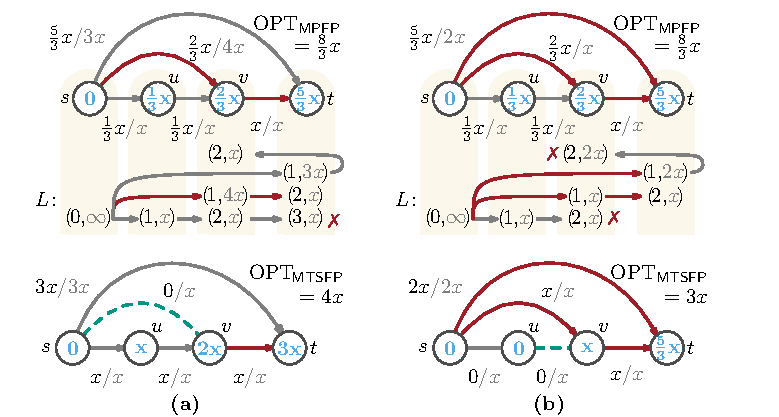
\includegraphics{switchplacement/figures/comparing_delta_theta_path.pdf}
    %
    \caption[An example and counterexample for the~\gls{dtp} calculation.]
    {%
    A network~\glssymbol{network} with four vertices and five edges, one
    generator~$\glssymbol{generators}=\{\source\}$, one
    consumer~$\glssymbol{consumers}=\{\sink\}$,
    capacities~\screentextcolor{KITblack50}{$\capacity(\vertexa,\vertexb)$}
    \mbox{(\screentextcolor{KITblack50}{gray})}, susceptance~$\glssymbol{susceptance}
    (\vertexa,\vertexb)=1$ for all $(\vertexa,\vertexb)\in\glssymbol{edges}$,
    and voltage angles~\screentextcolor{THETA}{$\vangle(\vertexa)$}
    (\screentextcolor{THETA}{blue} in the vertices) for all
    vertices~$\vertexa\in\vertices$. Note for the label calculation that the
    underlying graph~\graph is undirected. The algorithm computing the~\gls{dtp}
    saves a set of labels~\myhl{HiLi!50}{$\glssymbol{labels}$} for each vertex
    starting at vertex~\source with label~$(0,\infty)$. The 
    \screentextcolor{KITred}{red edges} represent the~\gls{dtp} from~\source
    to~\sink. (a)~The cross~\screentextcolor{KITred}{\ding{55}} means that the
    label~$(3,x)$ is dominated by the label~$(2,x)$ at vertex~\sink. In
    addition, it is not sufficient to compare only the voltage angle
    differences~\glssymbol{voltageangledifference}, since we would drop
    the~\gls{dtp} path~$[\source, (\source,\vertexb),\vertexb]$ at
    vertex~\vertexb, which would lead to incorrect results. Switching
    edge~$(\source,\vertexb)$ (\screentextcolor{KITgreen}{green dashed edge})
    results in a solution of the~\gls{mtsfp}. (b)~The~\gls{dtp} is not always
    unique. In addition, for general graphs the switched edge of the~\gls{mtsfp}
    is not always on the~\gls{dtp}. }%
    % 
    \label{fig:comparing_delta_theta_path} 
\end{figure}
% 
An~\source-\sink-network is often restricted (dominated) by the path with
the smallest voltage angle difference. However, it does not seem feasible to
give a general bound for that. %
The smallest voltage angle difference between a vertex~\vertexa and a
vertex~\vertexb is denoted by~$\glssymbol{voltageangledifferencemin}(\vertexa,\vertexb) \coloneqq
\min\glssymbol{voltageangledifference}\left(\fpath{}{\vertexa}
{\vertexb}\right)$ with $
\fpath{}{\vertexa}{\vertexb}\in\paths(\vertexa,\vertexb)$. 
% 
% 
We call the path that minimizes~$\glssymbol{voltageangledifference}(\fpath{}{\vertexa}{\vertexb})$
\acrlong{dtp} (\gls{dtp}) and denote it by~$\fpath{\dtp}{\vertexa}
{\vertexb}$. Its
value is
denoted by~$\opt_{\gls{dtp}}(\vertexa,\vertexb)$. 
%  
%
We are mainly interested in~\source-\sink-paths, since the power flows from
generators~\source to consumers~\sink.
% 
%%%%%%%%%%%%%%%%%%%%%%%%%%%%%%%%%% ALGORITHM %%%%%%%%%%%%%%%%%%%%%%%%%%%%%%%%%%%
%
% \wormhole{bit:ch:switching:sec:exploit_structural_characteristics:subsec:dtp:alg:shortest_theta_path}
\def\HiLi{\leavevmode\rlap{\hbox to \hsize{\color{HiLi}\leaders\hrule
height .9\baselineskip depth 1.3ex\hfill}}}
\begin{algorithm}[tb!]%
\SetAlgoLined
  % 
  % 
  \KwData{A network~$\glssymbol{network} = 
  (\glssymbol{graph},\glssymbol{generators},\glssymbol{consumers},\glssymbol{capacity},\glssymbol{susceptance})$.}
  % 
  \KwResult{$\fpath{\glssymbol{dtp}}{\source}{\sink}$,
  $\glssymbol{voltageangledifferencemin}(\source,t)$, and
  $\glssymbol{paretolabels}(\vertex)$ with~$\vertex\in\glssymbol{vertices}$.}
  % 
  % INITIALIZATION %%%%%%%%%%%%%%%%%%%%%%%%%%%%%%%%%%%%%%%%%%%%%%%%%%%%%%%%%%%%
  $\glssymbol{paretolabels}(\vertexa) \coloneqq \glssymbol{labels}(\vertexa)
  \coloneqq
  \emptyset \hspace{1em}\forall\vertexa\in\glssymbol{vertices}$%
  \Comment*{\color{KITblack30}Initialization}%
  \label{alg:initialization_begin}
  
  $\glssymbol{priorityqueue}\coloneqq\emptyset$\;
  
  $\glssymbol{labels}(\source) \coloneqq \left\{(0, \infty)\right\}$%
  \Comment*{\color{KITblack30} Special label for source~$\source$}%
  \label{ch:switching:sec:exploit_structural_characteristics:subsec:dtp:alg:shortest_theta_path:line:source_init}

  \screen{\HiLi}
  $\glssymbol{priorityqueue}.\myinsert\big((0,\infty),\source,\mathrm{key}((0,\infty))\big)$\; 
  \label{alg:initialization_end}
  %
  % LOOP UNTIL QUEUE IS EMPTY %%%%%%%%%%%%%%%%%%%%%%%%%%%%%%%%%%%%%%%%%%%%%%%%%
  \While(\Comment*[f]{\color{KITblack30}Visit all
  vertices}){$\glssymbol{priorityqueue}\not=\emptyset$} { % while
    % $\vertices:=\vertices\setminus\{\vertexa\}$\;
    %
    $(\glssymbol{label},\vertexa,\mathrm{key}) \coloneqq \glssymbol{priorityqueue}.\deleteMin()$\;
    \label{ch:switching:sec:exploit_structural_characteristics:subsec:dtp:alg:shortest_theta_path:line:min_key}
    $\glssymbol{paretolabels}(\vertexa) \coloneqq
    \glssymbol{paretolabels}(\vertexa) \cup \{
    \glssymbol{label} \}$\;
    \label{ch:switching:sec:exploit_structural_characteristics:subsec:dtp:alg:shortest_theta_path:line:paretolabels}
    % UPDATE ADJACENT VERTICES %%%%%%%%%%%%%%%%%%%%%%%%%%%%%%%%%%%%%%%%%%%%%%%%
    \For(\Comment*[f]{\color{KITblack30}Check adjacent vertices}){$\forall
    \{\vertexa,\vertexb\}\in\glssymbol{undirectededges}$
    \label{alg:check_adjacent_vertices}}{
    % 
      % MODIFIED UPDATE FUNCTION %%%%%%%%%%%%%%%%%%%%%%%%%%%%%%%%%%%%%%%%%%%%%%
      $\fmincapacity{}{\fpath{}{\source}{\vertexa,\vertexb}} \coloneqq
      \min\left(\glssymbol{label}[1],
      \capacity(\vertexa,\vertexb)
      \right)$\;
      % 
      \def\HiLi{\leavevmode\rlap{\hbox to \hsize{\color{HiLi}\leaders\hrule
      height 1.\baselineskip depth 1.70ex\hfill}}}
      \screen{\HiLi}
      $\labnew(\vertexb)\coloneqq\left(\glssymbol{label} [0]
            +\frac{1}{\glssymbol{susceptance}(\vertexa,\vertexb)},\fmincapacity{}{
                  \fpath{}{\source}{\vertexa,\vertexb}}\right)$\;
      % 
      \label{ch:switching:sec:exploit_structural_characteristics:subsec:dtp:alg:shortest_theta_path:line:update_function_alg}
      %
      % DECIDE WETHER UPDATE OR NOT %%%%%%%%%%%%%%%%%%%%%%%%%%%%%%%%%%%%%%%%%
      \def\HiLi{\leavevmode\rlap{\hbox to \hsize{\color{HiLi}\leaders\hrule
      height .8\baselineskip depth 1.3ex\hfill}}}
      \screen{\HiLi}
      \If{$\isReachable(\glssymbol{vertices}\setminus\{\vertexb\},\glssymbol{label},\source)$
        \label{ch:switching:sec:exploit_structural_characteristics:subsec:dtp:alg:shortest_theta_path:line:check_reachability}}
      {
        \uIf{$\labnew(\vertexb)\in\glssymbol{labels}(\vertexb)$
          \label{ch:switching:sec:exploit_structural_characteristics:subsec:dtp:alg:shortest_theta_path:line:check}}{
          $\parent(\labnew(\vertexb)) \coloneqq \parent(\labnew(\vertexb)) \cup 
          \{\glssymbol{label}\}$\;
        }
        \ElseIf{\kwnot $\glssymbol{labels}(\vertexb)$ \kwdominates $\labnew(\vertexb)$ 
          \label{ch:switching:sec:exploit_structural_characteristics:subsec:dtp:alg:shortest_theta_path:line:check_dominance}}
        {
          $\glssymbol{labels}(\vertexb).\deleteDominatedLabels(\labnew(\vertexb))$\;
          $\glssymbol{priorityqueue}.\deleteDominatedLabels(\labnew(\vertexb), \vertexb)$\;
            \label{ch:switching:sec:exploit_structural_characteristics:subsec:dtp:alg:shortest_theta_path:line:delete_dominated_Q}
          $\glssymbol{labels}(\vertexb).\myinsert(\labnew(\vertexb))$\;
            \label{ch:switching:sec:exploit_structural_characteristics:subsec:dtp:alg:shortest_theta_path:line:insert_L}
          $\glssymbol{priorityqueue}.\myinsert(\labnew(\vertexb),\vertexb,
            \mathrm{key}(\labnew(\vertexb)))$\;
            \label{ch:switching:sec:exploit_structural_characteristics:subsec:dtp:alg:shortest_theta_path:line:insert_Q}
          $\parent(\labnew(\vertexb)) \coloneqq \{\glssymbol{label}\}$\;
        } % else if
      } % if
    } % for
  } \vspace{-2mm} % while
  \Return{\hspace{-.08cm}$
    \left (
      \begin{tabular}{l}
      $\!\!\!\!\!\!~\fpath{\glssymbol{dtp}}{\source}{\sink}\coloneqq\getPaths
      (\source,\sink),\,\,$\Comment{
      \color{KITblack30}Build paths from \parent\hphantom{-}\!\!\!\!\!}\\ 
      $\!\!\!\!\glssymbol{voltageangledifferencemin}(\source,t)\coloneqq 
      \min_{\glssymbol{label}\in\glssymbol{paretolabels}(\sink)}\{\glssymbol{label}
      [0]\cdot\glssymbol{label} [1]\},\!\!\!$\\      % $\tree_{\dtp}:=\parent(\cdot),$ 
      $\!\!\!\glssymbol{paretolabels}(\cdot)$
      \end{tabular}
    \right )
  $
  }\;
  \caption{\acrlong{dtp}~(\gls{dtp}) Algorithm}%
\label{ch:switching:sec:exploit_structural_characteristics:subsec:dtp:alg:shortest_theta_path}%
\end{algorithm}% 
% 

Note that, unlike shortest paths, a~\gls{dtp} from~\source to~\sink via another
vertex~\vertexb and a~\gls{dtp} from~\source to~\vertexb may have no common
edges. For example in the top part
of~\cref{fig:comparing_delta_theta_path}\screen{a} a~\gls{dtp} to~\vertexb goes
via~\vertexa, but not the~\gls{dtp} to~\sink. To compute a~\gls{dtp} we
therefore minimize over two objectives~$\bnorm{\cdot}$
and~$\glssymbol{mincapacity}(\cdot)$. For this we perform a multi-objective
search, where we search for Pareto-optimal solutions, \ie, we look for paths
that are not dominated by other paths with regards to the objective functions
(in our case the susceptance norm~$\bnorm{\cdot}$ and minimum
capacity~$\glssymbol{mincapacity}(\cdot)$). Note that in general multi-objective
search is already~\NP-hard for two objective functions~\parencite{Gar79}
(see~\cref{ch:switching:sec:exploit_structural_characteristics:subsec:dtp:fig:non_poly_number_of_labels}).
%
\begin{definition}[Label Domination Criteria]
    % 
    Each~\source-\vertexa-path~$\pathu$ in~\glssymbol{network} defines a
    label~$\lab=(\bnorm{\pathu},\glssymbol{mincapacity}(\pathu))$ at~\vertexa.
    % 
    A label~$(\bnorm{\pathu_1}, \glssymbol{mincapacity}(\pathu_1))$
    \emph{dominates} another label~$(\bnorm{\pathu_2},
    \glssymbol{mincapacity}(\pathu_2))$ if
    $\bnorm{\pathu_1}\leq\bnorm{\pathu_2}$ and
    $\glssymbol{mincapacity}(\pathu_1)\le\glssymbol{mincapacity}(\pathu_2)$. 
    % 
\end{definition}
% 
% 
The Pareto set~$\glssymbol{paretolabels}(\vertexa)$ of labels at a
vertex~$\vertexa\in\glssymbol{vertices}$ is then defined as the set of
nondominated labels of all~\source-\vertexa-paths
(\cref{ch:switching:sec:exploit_structural_characteristics:subsec:dtp:alg:shortest_theta_path:line:paretolabels}).
%
These Pareto sets can be computed by a natural extension of Dijkstra's algorithm
(see~\cref{ch:switching:sec:exploit_structural_characteristics:subsec:dtp:alg:shortest_theta_path})
known as the
% 
\emph{multi-criteria shortest-path} algorithm~\parencite{MARTINS1984236}. At
each vertex~$\vertexa\in\glssymbol{vertices}$ a set of nondominated labels~$
\glssymbol{labels}(\vertexa)$
% 
is stored. Note that in general, each label may correspond to 
% 
multiple~\source-\vertexa-paths. As it is necessary to represent all these
paths, we store for each label a set of~\parent-pointers. The latter point to
labels that correspond to paths shortened by one vertex. The merging of labels
ensures the polynomial size of label sets.

%
The labels in the priority queue~\glssymbol{priorityqueue} are compared
by~$\bnorm{\cdot}$.
% 
% 
At the beginning of each iteration a label with the minimum susceptance norm is
extracted from~\glssymbol{priorityqueue}. This label belongs to a
vertex~\vertexa. Then, new labels for all neighbors of~\vertexa are computed
(\cref{ch:switching:sec:exploit_structural_characteristics:subsec:dtp:alg:shortest_theta_path:line:update_function_alg}). First, it is checked
whether there is a path~$\fpath{}{\source}{\vertexa}$ that corresponds to~
\glssymbol{label} and does not contain the neighbor~\vertexb
(\cref{ch:switching:sec:exploit_structural_characteristics:subsec:dtp:alg:shortest_theta_path:line:check_reachability},
\cref{ch:switching:sec:exploit_structural_characteristics:subsec:reachibility_test}). Extending this path to~\vertexb then
still gives a simple path. If the computed label already exists
in~$\glssymbol{labels}(\vertexb)$, the~\parent-pointers are updated. Otherwise,
if it is not dominated, it is added to~$\glssymbol{labels}(\vertexb)$
and~\glssymbol{priorityqueue}
(\cref{ch:switching:sec:exploit_structural_characteristics:subsec:dtp:alg:shortest_theta_path:line:insert_L,ch:switching:sec:exploit_structural_characteristics:subsec:dtp:alg:shortest_theta_path:line:insert_Q}).
Before that, all labels dominated by the new labels are removed. Here, only
labels at the same vertex are considered, \ie, in
\cref{ch:switching:sec:exploit_structural_characteristics:subsec:dtp:alg:shortest_theta_path:line:delete_dominated_Q} only the dominated labels
at~\vertexb are removed.
%
\begin{lemma}%
\cref{ch:switching:sec:exploit_structural_characteristics:subsec:dtp:alg:shortest_theta_path} computes a correct~\acrlong{dtp}~(\gls{dtp}).
\label{lem:correctDTP}
\end{lemma}%
% 
Note that the proof for the next lemma is based on the proof for the 
\emph{multi-criteria shortest-path} algorithm by~\textcite{MARTINS1984236}.
% 
\begin{proof}
    At any step of~\cref{ch:switching:sec:exploit_structural_characteristics:subsec:dtp:alg:shortest_theta_path} there is a set of
    labels~$\glssymbol{labels}(\vertexa)$ associated with each vertex
    $\vertexa\in\glssymbol{vertices}$. We first show that at any step no label
    in~$\glssymbol{labels}(\vertexa)$ is dominated by any other label in the same
    set.
    %
    % Base case
    %
    After the initialization there is only one label. Hence, it is not
    dominated. 
    %
    % Induction step 
    %
    %%%%%%%%%%%%%%%%%%%%%%%%%%%%%%%%%% FIGURE %%%%%%%%%%%%%%%%%%%%%%%%%%%%%%%%%%
    \begin{figure}
    % 
    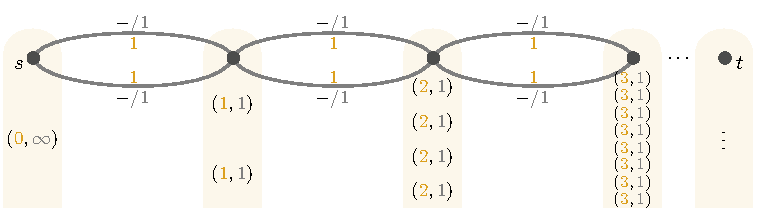
\includegraphics[page=1]{switchplacement/figures/DTP_non_poly_num_labels.pdf}
    % 
    \caption[An example, where the~\gls{dtp} produces exponential many labels.]
    {%
    An example, where the~\gls{dtp} produces exponential many labels. The edges
    are given with
    the~\textcolor{SUSCEPTANCE}{susceptances~\glssymbol{susceptance}} and
    \textcolor{CAPACITY}{capacities~\glssymbol{capacity}}. The sets of labels
    are marked at the vertices. The number of labels increases from the
    source~\source for each vertex in the chain exponentially by either choosing
    the upper or lower edge.
    }%
    % 
    \label{ch:switching:sec:exploit_structural_characteristics:subsec:dtp:fig:non_poly_number_of_labels}
    % 
    \end{figure}
     
    Suppose that there are no dominated labels in any label set before an iteration.
    We show that this property still holds after the iteration.
    First, a label~$(\bnorm{\fpath{}{\source}{\vertexa}},$ 
    $\glssymbol{mincapacity}(\fpath{}{\source}{\vertexa}))$ with the 
    minimum susceptance norm among all labels in~\glssymbol{priorityqueue} is
    dequeued (\cref{ch:switching:sec:exploit_structural_characteristics:subsec:dtp:alg:shortest_theta_path:line:min_key}). This label
    corresponds to a path~$\fpath{}{\source}{\vertexa}$ from~\source 
    to~\vertexa. Then, the labels for neighbors of~\vertexa are computed
    (\cref{ch:switching:sec:exploit_structural_characteristics:subsec:dtp:alg:shortest_theta_path:line:update_function_alg} based
    on~\cref{eq:update_function}). Since these labels are only added if they are
    not dominated and labels dominated by them are removed
    from~$\glssymbol{labels}(\vertexb)$, the label sets still do not contain
    dominated labels. Moreover, the new labels also correspond to simple paths
    as it is tested whether~\vertex already lies
    on~$\fpath{}{\source}{\vertexa}$. Note that previously extracted labels
    from~\glssymbol{priorityqueue} are not removed since their susceptance norm
    is less than the one of~$\lab_\textrm{new}(\vertexb)$. In particular, all
    labels extracted from~\glssymbol{priorityqueue} will be present in the final
    label sets.

    Secondly, we prove that in the end we have~$\glssymbol{paretolabels}
    (\vertexb)\subseteq\glssymbol{labels}(\vertexb)$ for
    all~$\vertexb\in\glssymbol{vertices}$. Assume that this was not the case.
    Then, there is a label~$\lab\in\glssymbol{paretolabels}(\vertexb)$ that is
    not included in~$\glssymbol{labels} (\vertexb)$ for
    some~$\vertexb\in\glssymbol{vertices}$. We pick such a label with the
    minimum susceptance norm. This label corresponds to a path~$\pathu(\source,
    \vertexb)$. Denote the vertex before~\vertexb by~\vertexa. 
    Since the subpath~$\pathu(\source, \vertexa)$ from~$\source$ to~$\vertexa$ has~$
    \bnorm{\pathu(\source,\vertexa)} < \bnorm{\pathu(\source,\vertexb)}$, the 
    label for this subpath is present in~$\glssymbol{labels}(\vertexa)$. But in the
    iteration in which this label was processed, all neighbors of~\vertexa were
    explored. In particular, the label~\lab for~\vertexb was computed and added
    to~$\glssymbol{labels}(\vertexb)$. Moreover, it was never removed
    from~$\glssymbol{labels}(\vertexb)$ later, since it is not dominated. This
    contradicts the existence of~\lab.
    % 
    Since~$\glssymbol{paretolabels}(\vertexa)\subseteq\glssymbol{labels}(\vertexa)$
    and~$\glssymbol{labels}(\vertexa)$ contains no dominated labels, we
    conclude~$\glssymbol{paretolabels}(\vertexa)=\glssymbol{labels}(\vertexa)$.
    The~\gls{dtp} is then computed by minimizing
    over~$\glssymbol{labels}(\sink)$.
\end{proof}
% 
%%%%%%%%%%%%%%%%%%%%%%%%%%%%%%%%%% FIGURE %%%%%%%%%%%%%%%%%%%%%%%%%%%%%%%%%%
\begin{figure}[tb!]
    \centering
    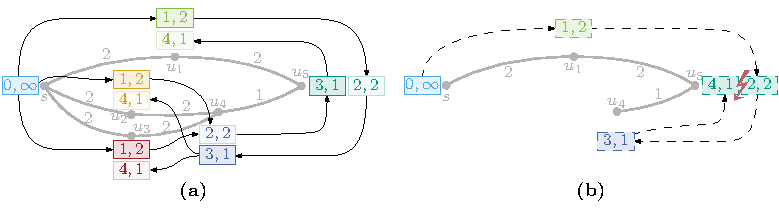
\includegraphics{switchplacement/figures/dtp_labels_to_colored_dag.pdf}
    %
    \caption[The directed label graph after an {\gls{dtp}}-algorithm
    execution.]{%
    A network~\glssymbol{network} and the corresponding directed graph on
    the labels computed during the execution of the {\gls{dtp}}-algorithm.
    All edges~$(\vertexa,\vertexb)\in\glssymbol{edges}$ have
    susceptance~$\textcolor{SUSCEPTANCE}{\glssymbol{susceptance}\equiv 1}$.
    Two labels have the same color if and only if they belong to the same
    vertex in~\glssymbol{network}. (a) To test whether the label~$(4,1)$
    at~$\vertexa_3$ shall be inserted into the graph, we search for a
    rainbow path from the label at~\source to the new label~$(4,1)$. The
    slightly colored labels produce no~\gls{dtp} from that particular
    vertex. (b) The rainbow path avoids cycles and ensures that the paths
    remain simple. 
    }%
    % 
    \label{ch:switching:sec:exploit_structural_characteristics:fig:dtp_labels_to_colored_dag}
\end{figure}
% 
A counterexample for monotone voltage angle paths is given in~\cref{ch:switching:sec:exploit_structural_characteristics:fig:labels_and_does_not_lie_on_monoton_theta_paths} 
confirming~\cref{ch:switching:sec:exploit_structural_characteristics:lem:dtp-monotony}.
%
\begin{lemma}
    The~\acrlong{dtp} (\gls{dtp}) is not necessarily on a monotone voltage
    angle path.
    % 
    \label{ch:switching:sec:exploit_structural_characteristics:lem:dtp-monotony}
\end{lemma}  
% 
%%%%%%%%%%%%%%%%%%%%%%%%%%%%%%%%%%%%%%%%%%%%%%%%%%%%%%%%%%%%%%%%%%%%%%%%%%%%%%%%
\subsection{DTP without Merging the Labels}
\label{ch:switching:sec:exploit_structural_characteristics:subsec:DTP_without_label_merging}
%%%%%%%%%%%%%%%%%%%%%%%%%%%%%%%%%%%%%%%%%%%%%%%%%%%%%%%%%%%%%%%%%%%%%%%%%%%%%%%%
% 
The~\cref{ch:switching:sec:exploit_structural_characteristics:subsec:dtp:alg:shortest_theta_path}
for the~\gls{dtp} can be implemented using the merging of equivalent labels or
without merging. Neglecting the merging of labels would mean that we
remove~\cref{ch:switching:sec:exploit_structural_characteristics:subsec:dtp:alg:shortest_theta_path:line:check_reachability}
that avoids cycles
and~\cref{ch:switching:sec:exploit_structural_characteristics:subsec:dtp:alg:shortest_theta_path:line:check}
that merges the labels. Thus, the reachability check is neglected, but we have
to add cycle checks that are also done by the reachability test
(see~\cref{ch:switching:sec:exploit_structural_characteristics:subsec:reachibility_test}).
The implementation stores a set of visited vertices~$\glssymbol{vertices}'$ for
every label. Using a simple union operation on these set, we are able to check
for cycles. In worst-case we have to
save~$\bigO(\fmagnitude{\glssymbol{vertices}})$ elements per vertex in that set.
Thus, a label consists in that case of~$(\bnorm{\cdot}, \glssymbol{mincapacity}
(\cdot),\glssymbol{vertices}')$. Note that this method can lead to exponential
many labels as exemplified
in~\cref{ch:switching:sec:exploit_structural_characteristics:subsec:dtp:fig:non_poly_number_of_labels}.
However, the reachability test leads to an exponential running time
(see~\cref{ch:switching:sec:exploit_structural_characteristics:subsec:reachibility_test,ch:switching:sec:exploit_structural_characteristics:eq:runtime_exp_DTP}).% %%%%%%%%%%%%%%%%%%%%%%%%%%%%%%%%%%%%%%%%%%%%%%%%%%%%%%%%%%%%%%%%%%%%%%%%%%%%%%%%
\subsection{Reachability Test}
\label{ch:switching:sec:exploit_structural_characteristics:subsec:reachibility_test}
%%%%%%%%%%%%%%%%%%%%%%%%%%%%%%%%%%%%%%%%%%%%%%%%%%%%%%%%%%%%%%%%%%%%%%%%%%%%%%%%
% 
\cref{ch:switching:sec:exploit_structural_characteristics:subsec:dtp:alg:shortest_theta_path}
repeatedly tests whether the new labels correspond to simple paths in the
network
(\cref{ch:switching:sec:exploit_structural_characteristics:subsec:dtp:alg:shortest_theta_path:line:check_reachability}
of
\cref{ch:switching:sec:exploit_structural_characteristics:subsec:dtp:alg:shortest_theta_path}).
For this it is checked whether the label at vertex~\source is reachable
from~\vertexa via
\parent-pointers from the label~\glssymbol{label} when all labels at~\vertexb
are ignored. The labels and the pointers together form a directed acyclic graph,
where the labels have the same color if and only if they belong to the same
vertex in network~\glssymbol{network}
(see~\cref{ch:switching:sec:exploit_structural_characteristics:fig:dtp_labels_to_colored_dag}).
We call a path whose vertices all have different colors a \emph{rainbow path}.
%
%%%%%%%%%%%%%%%%%%%%%%%%%%%%%%%%%%%% FIGURE %%%%%%%%%%%%%%%%%%%%%%%%%%%%%%%%%%%%
\begin{figure}[t!]
  \centering
  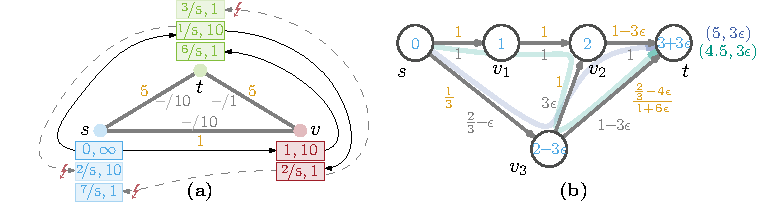
\includegraphics{switchplacement/figures/labels_and_does_not_lie_on_monoton_theta_paths.pdf}
  %
  \caption[\gls{dtp} problematic cases.]{%
  The graphs represent two problematic cases. (a) An example that shows that it
  does not suffice that the labels consist
  of~$(\bnorm{\cdot},\glssymbol{mincapacity}(\cdot))$, but has to include the
  set of visited vertices~$\glssymbol{vertices}'$. (b) Shows an example that
  the~\gls{dtp} is not necessarily on a monotone voltage angle path. Let~$0 <
  \epsilon \ll \nicefrac{2}{3}$ then the green path represents the~\gls{dtp}
  from~\source to~\sink. }%
  % 
  \label{ch:switching:sec:exploit_structural_characteristics:fig:labels_and_does_not_lie_on_monoton_theta_paths}
\end{figure}
%
\begingroup
    %%%%%%%%%%%%%%%%%%%%%%%%%%%%%%%%%%% Problem %%%%%%%%%%%%%%%%%%%%%%%%%%%%%%%%%%%%
\begin{problem}[framed]{\acrlong{strp}~$\gls{strp}(
\glssymbol{graph},c,\source,\sink)$}
    Instance: & A directed acyclic graph~$\glssymbol{graph} =
    (\glssymbol{vertices},\glssymbol{edges})$, a
    coloring~$\col\colon\glssymbol{vertices}\to\naturals$, and $\source,
    \target\in\glssymbol{vertices}$.\\
    % 
    Question: & Is there an~\source-\target-path~$\pathu$ in~\glssymbol{graph}
    such that all vertices of~$\pathu$ have different colors?
\end{problem} 
    \label{ch:switching:problems:Rainbow_s_t_path-Decision_Problem}
\endgroup
%
An algorithm to test whether there is a~\acrlong{strp} (\gls{strp}) in
undirected graphs was presented by~\textcite[Theorem~11]{Uch13}. It runs
in~$\bigO(k2^k \fmagnitude{\glssymbol{edges}}\fmagnitude{\glssymbol{vertices}})$
time, where~$k$ is the number of colors, $\fmagnitude{\glssymbol{edges}}$ the
number of edges, and~$\fmagnitude{\glssymbol{vertices}}$ the number of vertices
in~\glssymbol{graph}. We give a different algorithm for directed graphs, which
can be implemented to run in~$\bigO(k2^k\fmagnitude{\glssymbol{edges}})$ time.
The main work is done
by~\cref{ch:switching:sec:exploit_structural_characteristics:alg:compute_colors}.
It additionally gets a set~$\forbidden$ of forbidden colors as input and ignores
all vertices of these colors. To decide whether there is a rainbow path from a
vertex~\source to a vertex~\target, we initially set~\forbidden to~$\emptyset$.
We compute for each vertex~\vertex a set of
colors~$\colorlabels_\forbidden(\vertex)$. A color~\col is in the
set~$\colorlabels_\forbidden(\vertex)$ if and only if any
rainbow~\source-\vertex-path~$\fpath{}{\source}{\vertex}$ contains a vertex with
color~\col with the additional constraint that no vertex of~$\fpath{}{\source}
{\vertex}$ is colored with a color in~$\forbidden$
(in~\cref{ch:switching:sec:exploit_structural_characteristics:alg:compute_colors}~\cref{ch:switching:sec:exploit_structural_characteristics:alg:compute_colors:5,ch:switching:sec:exploit_structural_characteristics:alg:compute_colors:6}).
For each vertex~\vertexb and all its incoming edges~$(\vertexa,\vertexb)$ we
recursively compute all necessary colors for the rainbow paths to $\vertexa$
such that~$\col(\vertexb)$ is forbidden. The
set~$\colorlabels_\forbidden(\vertexb)$ is then equal to the intersection of
these color sets together with~$\col(\vertexb)$. Throughout the algorithm we
use~$\naturals$ to indicate that there is no rainbow path with the given
restrictions.

During the
execution~\cref{ch:switching:sec:exploit_structural_characteristics:alg:compute_colors}
may be called several times with the same parameters. To speed up the
computation one may store the results instead of recomputing them every time.
Further, we find a relation between~$\colorlabels_\forbidden(\vertex)$
and~$\colorlabels_{\forbidden'}(\vertex)$ for a vertex~\vertex and two sets of
forbidden colors~\forbidden and~$\forbidden'$. If every color of a vertex
before~\vertex in the topological order is either both in~\forbidden
and~$\forbidden'$ or neither in~\forbidden nor~$\forbidden'$, we
have~$\colorlabels_\forbidden(\vertex) =
\colorlabels_{\forbidden'}(\vertex)$. In particular, if no vertex
before~$\vertex$ is colored by any color in~$\forbidden$, we
have~$\colorlabels_\forbidden(\vertex)=\colorlabels_\emptyset(\vertex)$. This
property can also be used to reduce the number of recursive calls.

Alternatively, the set of colors~$\colorlabels_\forbidden(\vertex)$ at a
vertex~\vertex can be computed by traversing all paths from~\source to~\vertex,
checking if no two vertices are colored the same and finally taking the common
colors of all rainbow paths. This may be faster if there are only
few~\source-\vertex-paths or if many of the paths can be eliminated quickly
because they are not rainbow paths.
% 
%%%%%%%%%%%%%%%%%%%%%%%%%%%%%%%%%% ALGORITHM %%%%%%%%%%%%%%%%%%%%%%%%%%%%%%%%%%%
\begin{algorithm}[tb!]
    \SetAlgoLined
    % 
    \KwData{%
        A directed label network~$\coloredgraph=(\glssymbol{graph}=
        (\glssymbol{vertices},\glssymbol{edges}),\col, \source)$,
        where~$\col\colon\glssymbol{vertices}\to\naturals$ is the coloring
        and~$\source\in\glssymbol{vertices}$ is the fixed source of the network,
        $\vertexb\in\glssymbol{vertices}$, and a
        set~$\forbidden\subseteq\naturals$ of forbidden colors. }
    % 
    \KwResult{%
        The intersection of the colors of all rainbow 
        \source-\vertexb-paths, or~$\naturals$ if there are no such paths. }

    \lIf(\Comment*[f]{\color{KITblack30}Not a rainbow path?})
        {$\col(\vertexb)\in\forbidden$}%
    {%
        \Return{\naturals}
        \label{ch:switching:sec:exploit_structural_characteristics:alg:compute_colors:1}
    } % if
    \lIf(\Comment*[f]{\color{KITblack30}Base case})
        {$\source=\vertexb$}%
    {%
        \Return{$\{\col(\source)\}$}%
        \label{ch:switching:sec:exploit_structural_characteristics:alg:compute_colors:2}
    } % if
    $\colorlabels_\forbidden(\vertexb) \coloneq \naturals$\;
    \label{ch:switching:sec:exploit_structural_characteristics:alg:compute_colors:3}
    %  
    \For(\Comment*[f]{\color{KITblack30}All incoming edges into~\vertexb}){
        $(\vertexa,\vertexb)\in\edges$
    }{
        $C'\coloneqq\computeColors\left(\coloredgraph, \vertexa, 
        \forbidden\cup\{\col(\vertexb)\}\right)$\Comment*
        {\color{KITblack30}Incoming cut}
        \label{ch:switching:sec:exploit_structural_characteristics:alg:compute_colors:5}
        % 
        $\colorlabels_\forbidden(\vertexb) \coloneqq 
        \colorlabels_\forbidden(\vertexb) \cap C'$\;
        \label{ch:switching:sec:exploit_structural_characteristics:alg:compute_colors:6}
    } % for
    $\colorlabels_\forbidden(\vertexb) \coloneqq \colorlabels_\forbidden
    (\vertexb) \cup \{\col(\vertexb)\}$\;
    \label{ch:switching:sec:exploit_structural_characteristics:alg:compute_colors:8}
    % 
    \Return{$\colorlabels_\forbidden(\vertexb)$}\;
    \label{ch:switching:sec:exploit_structural_characteristics:alg:compute_colors:9}
    % 
    \caption{computeColors}
    % 
    \label{ch:switching:sec:exploit_structural_characteristics:alg:compute_colors}
\end{algorithm}
% 
%%%%%%%%%%%%%%%%%%%%%%%%%%%%%%%%%%%%%%%%%%%%%%%%%%%%%%%%%%%%%%%%%%%%%%%%%%%%%%%%
%%%%%%%%%%%%%%%%%%%%%%%%%%%%%%%%%%%%%%%%%%%%%%%%%%%%%%%%%%%%%%%%%%%%%%%%%%%%%%%%
\subsection{Analyses of the DTP}
\label{ch:switching:sec:exploit_structural_characteristics:subsec:dtp_analyses}
%%%%%%%%%%%%%%%%%%%%%%%%%%%%%%%%%%%%%%%%%%%%%%%%%%%%%%%%%%%%%%%%%%%%%%%%%%%%%%%%
% 
Examples of this algorithm are shown 
% 
in the upper part of~\cref{fig:comparing_delta_theta_path}\screen{a}
and~\screen{b}. Note that there are at most~$\fmagnitude{\glssymbol{edges}}$
different values of~$\glssymbol{mincapacity}(\cdot)$
since there are at most~$\fmagnitude{\glssymbol{edges}}$ different labels saved per vertex
assuming that we merge and have a penrose-minor free graph with direction. This
bound is tight. Consider for example two vertices with~$\fmagnitude{\glssymbol{edges}}$
parallel lines, where line~$i$ has capacity~$i$ and
susceptance~$\nicefrac{1}{i}$.
%
\begin{lemma}
  For each~$\vertexa\in\glssymbol{vertices}$ we have~$\fmagnitude{
    \glssymbol{labels}(\vertexa)}\le\fmagnitude{\glssymbol{edges}}$.
  \label{ch:switching:sec:exploit_structural_characteristics:lem:label_set_bound}
\end{lemma}
%
Note that for arbitrary graphs the labels are of the form~$(\bnorm{\cdot},
\glssymbol{mincapacity}(\cdot),\glssymbol{vertices}')$, which results in
exponential many
labels. The non-negativity of the susceptance norm and capacity implies that
processed labels~$\glssymbol{paretolabels}(\cdot)$ will not be removed. This is
denoted as \emph{label setting}. In contrast, negativity would imply that there
may exist a path such that processed labels have to be updated by labels of
vertices on the negative path. In addition, all adjacent labels of the updated
labels have to be corrected and so forth. Algorithms working like this are
called \emph{label correcting} and do not perform as efficiently as label
setting algorithms.
% 
The running time
of~\cref{ch:switching:sec:exploit_structural_characteristics:subsec:dtp:alg:shortest_theta_path}
depends on the subroutine \texttt{isReachable} for which no polynomial bound is
known. Note that these tests are easy for labels that correspond to exactly one
path, \ie, labels that were not merged. On realistic power grid instances the
algorithm performs well since merging is rare.
% 
If we use a Fibonacci-heap~\glssymbol{priorityqueue} to store labels, the
operation~\myinsert is in~$\bigO(1)$, \deleteMin is amortized in~$\bigO(\log
\fmagnitude{\glssymbol{vertices}})$~\parencite{715934}, \deleteDominatedLabels is
in~$\bigO(\fmagnitude{\glssymbol{edges}})$, and~\isReachable
(see~\cref{ch:switching:sec:exploit_structural_characteristics:subsec:reachibility_test})
runs in~$\bigO (2^{\fmagnitude{\glssymbol{vertices}}} 
\fmagnitude{\glssymbol{vertices}}\cdot\fmagnitude{\glssymbol{edges}})$
time. The initialization is in~$\bigO(\fmagnitude{\glssymbol{vertices}})$ time
(\crefrange{alg:initialization_begin}{alg:initialization_end}). There
are~$\bigO(\fmagnitude{\glssymbol{vertices}}\cdot\fmagnitude{\glssymbol{edges}})$
\deleteMin operation, since every vertex can have up
to~$\fmagnitude{\glssymbol{edges}}$ labels. There
arise~$\bigO(\fmagnitude{\glssymbol{edges}}^2)$ operations of all other methods, since we
do these operation for all incident
edges~$\sum_{\vertexa\in\glssymbol{vertices}}
\deg(\vertexa) = 2\fmagnitude{\glssymbol{edges}}$~\parencite{Eul36}
(\cref{alg:check_adjacent_vertices}) and each vertex can have at
most~$\fmagnitude{\glssymbol{edges}}$ labels. Thus, the algorithm runs in time% 
% 
% 
\begin{align}
T\coloneq&\,\bigO\big(\fmagnitude{\glssymbol{vertices}}\cdot
\fmagnitude{\glssymbol{edges}}\cdot
T_{\deleteMin}
  + \fmagnitude{\glssymbol{edges}}^2\cdot \notag\\ &\left( T_{\myinsert} + T_{\isReachable}
    + T_{\deleteDominatedLabels} \right)
\big)\\
% 
=&\,\bigO\left(\fmagnitude{\glssymbol{vertices}}\cdot\fmagnitude{\glssymbol{edges}}\cdot
\log \fmagnitude{\glssymbol{vertices}} +
  2^{\fmagnitude{\glssymbol{vertices}}}\fmagnitude{
  \glssymbol{vertices}}\cdot\fmagnitude{\glssymbol{edges}}^3\right).
  % 
  \label{ch:switching:sec:exploit_structural_characteristics:eq:runtime_exp_DTP}
  %
%
\end{align}
% 
The following lemma results directly from the previous discussion.
% 
\begin{lemma}
  
\cref{ch:switching:sec:exploit_structural_characteristics:subsec:dtp:alg:shortest_theta_path}
runs in~$\bigO\left(2^{\fmagnitude{\glssymbol{vertices}}}\fmagnitude{\glssymbol{vertices}}\cdot\fmagnitude{\glssymbol{edges}}^3\right)$ time.
\end{lemma}
% 
% 
On general graphs we cannot assume that the switched edges are either tight
edges (\ie, bottleneck edges that are congested) or on the~\gls{dtp}
(in~\cref{fig:comparing_delta_theta_path}\screen{b} edge~$(\vertexa,\vertexb)$
is not on the~\gls{dtp}).
% 
%
In the following, we restrict our graph classes of the
network~\glssymbol{network} to~\source-\sink-networks (\ie, there is only
one~$\source\in\glssymbol{generators}$ and one~$\sink\in\glssymbol{consumers}$)
and try to solve the~\gls{mtsfp} on them. We identify structures, where
it is easy to switch. The following lemma shows at which point it is beneficial
to switch on simple cycles.
%
%%%%%%%%%%%%%%%%%%%%%%%%%%%%%%%%%%%% LEMMA %%%%%%%%%%%%%%%%%%%%%%%%%%%%%%%%%%%%
\begin{lemma}
  Let~\glssymbol{network} be a simple cycle with one generator~\source and one
  consumer~\sink, and let~$
  \fpath{}{\source}{\sink}\in\paths(\source,\sink)\setminus\fpath{\gls{dtp}}
  {\source}{\sink}$. The Braess's Paradox exists if and only
  if~$~\opt_{\gls{mpfp}}(\fpath{}{\source}{\sink})$ $>
  \opt_{\gls{mpfp}}(\glssymbol{network})$.
  % 
  \label{ch:switching:sec:exploit_structural_characteristics:lem:braess-paradox-path-cycle}
\end{lemma}
%  
%
\begin{proof}
%
It suffices to show that removing
edge~$\edge_{\min}(\fpath{\gls{dtp}}{\source}{\sink})\coloneqq
\argmin_{\edge\in\fpath{\gls{dtp}}{\source}{\sink}}\capacity(\edge)$ results
in~$\opt_{\gls{mpfp}}(\glssymbol{network}-\{\edge_{\min}\}) > \opt_{
\gls{mpfp}} (\glssymbol{network})$ and thus,
it holds~$\opt_{\gls{mtsfp}}(\glssymbol{network}) > \opt_{\gls{mpfp}}(
\glssymbol{network})$.
% 
The flow on the path~$\fpath{}{\source}{\sink}$ is defined by the
ratio~$\nicefrac{
\glssymbol{voltageangledifference}(\fpath{}{\source}{\sink})}{\bnorm{\fpath{}{\source}{\sink}}
}$ (\cref{ch:switching:sec:model:eq:KVL_dc_approx,eq:bnorm}). 
% 
The smallest voltage angle difference~$\glssymbol{voltageangledifferencemin}(\source,\sink)$
restricts the flow on the other path~$
\fpath{}{\source}{\sink}$. Thus, the term~$\nicefrac{
\glssymbol{voltageangledifferencemin}(\source,\sink)}{\bnorm{\fpath{}{\source}{\sink}}
}$ is the maximum possible flow on path~$\fpath{}{\source}{\sink}$.
%
% 
The value $\opt_{\gls{mpfp}}(\fpath{}{\source}
{\sink}) > \opt_{\gls{mpfp}}(\glssymbol{network})$ holds if and only if
% 
\begin{align*}
\frac{\glssymbol{voltageangledifference}(\fpath{}{\source}{\sink})}{\bnorm{\fpath{}{\source}{\sink}}} 
%
& >
%
\glssymbol{voltageangledifferencemin}(\source,\sink)
\cdot
\frac{\bnorm{\fpath{}{\source}{\sink}}
+ 
\bnorm{\fpath{\gls{dtp}}{\source}{\sink}}}
%
{\bnorm{\fpath{}{\source}{\sink}}
\cdot\bnorm{\fpath{\gls{dtp}}{\source}{\sink}}}.
%
% 
\end{align*}
Thus, switching an edge~$\edge_{\min}$
on~$\fpath{\gls{dtp}}{\source}{\sink}$
increases the total flow on the cycle and makes switching beneficial.
\end{proof}
% 
% 
We now generalize this result to a more complex graph class. Following the
construction in~\cref{ch:switching:sec:network_modeling}, we assume that all
generator and consumer vertices have degree~$1$. A diamond graph is a simple
graph on four vertices and five edges consisting of two triangle facets
identified along an edge. Moreover, we denote its degree-$3$ vertices as
\emph{girdle} vertices and its degree-2 vertices as its \emph{tip} vertices.
Furthermore, we call the combination of a \emph{kite} and a \emph{dart} graph
representing both diamond graphs with an additional edge on one of the tip and
the girdle vertices, respectively, a \emph{penrose} graph
(\cref{ch:switching:sec:exploit_structural_characteristics:fig:forbidden_minor}).
These additional edges basically represent either a generator edge or a consumer
edge, but not both the same. We emphasize this by the following definition.
% 
%%%%%%%%%%%%%%%%%%%%%%%%%%%%%%%%%%%% FIGURE %%%%%%%%%%%%%%%%%%%%%%%%%%%%%%%%%%%%
\begin{figure}[t!]
  \centering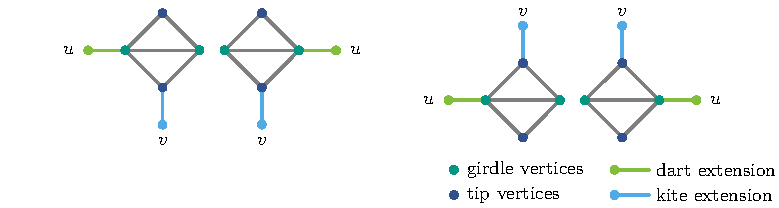
\includegraphics{switchplacement/figures/forbidden_minor.pdf}
  %
  \caption[A description of penrose-minors.]{All cases show penrose-minors,
  where~\vertexa and~\vertexb are either generators or consumers, but not both
  the same. They are a combination of a \screentextcolor{KITcyanblue}{kite
  graph} (\ie, diamond graph with an additional edge on one of the
  \screentextcolor{KITseablue}{tip vertices}) and
  a~\screentextcolor{KITpalegreen}{dart graph} (\ie, diamond graph with an
  additional edge on one of the
  \screentextcolor{KITgreen}{girdle vertices}).  
  }%
  \label{ch:switching:sec:exploit_structural_characteristics:fig:forbidden_minor}
\end{figure}
% 
\begin{definition}[Penrose Graph]
    A \emph{penrose} graph is a kite graph with an additional edge incident to
    one of the girdle vertices, or similarly, a dart graph with an additional
    edge on one of the tip vertices.
    % 
    \label{ch:switching:sec:exploit_structural_characteristics:def:penrose-graph}
\end{definition}
% 
A \emph{minor} of a network~\glssymbol{network} is obtained
from~\glssymbol{network} by contracting and deleting edges, as well as deleting
isolated vertices (\ie, vertices without incident edges).
% 
A~\emph{penrose-minor-free graph} is a graph 
% 
without a penrose graph as a minor.
%

In the following, we consider penrose-minor-free graphs with one
generator~\source and one consumer~\sink. Note that each block, \ie, a maximal
biconnected subgraph, of such graphs consist of one or more parallel paths. The
start and end vertices of the paths act as generator and consumer for the block.
Note that the blocks can be considered separately. Let~\block be a block
and~\vertexa and~\vertexc the start and end vertices of its paths. The flow
value~\glssymbol{flowvalue} of an~\gls{mpf} from~\vertexa to~\vertexc is
%
%%%%%%%%%%%%%%%%%%%%%%%%%%%%%%%%%%% EQUATION %%%%%%%%%%%%%%%%%%%%%%%%%%%%%%%%%%%
% 
$
% 
%
%
\glssymbol{flowvalue} = 
%%%%%%%
\glssymbol{voltageangledifferencemin}(\vertexa, \vertexc)
%
\cdot
%
\sum_{\pathu\in\glssymbol{pathset}(\vertexa,\vertexc)} 
\frac{1}{\bnorm{\pathu}}.%
%
$
%
To increase the flow value, either of the factors has to be increased. Switching
cannot increase the sum, but only the angle difference on the~\gls{dtp}. Thus,
the following result holds.
% 
\begin{lemma}
    Switching on~penrose-minor-free graphs is only beneficial
    on~\gls{dtp}{s}.
    % 
    \label{ch:switching:sec:exploit_structural_characteristics:lem:switching_in_DTP}
\end{lemma}
% 
From~\cref{ch:switching:sec:exploit_structural_characteristics:lem:switching_in_DTP}
we know that we only need to consider edges on a~\gls{dtp} for switching.
In~\cref{ch:switching:sec:exploit_structural_characteristics:alg:msf_series_parallel_structures}
for each block~\block\ we remove the edge with the smallest capacity
on~$\fpath{\gls{dtp}}{\source}{\sink}$ in~\block and update
the~$\gls{dtp}(\source,\sink)$. If we get a better value
for~\glssymbol{flowvalue}, we save it. We repeat this procedure until there is
no path from~\source to~\sink.
% 
The correctness of~\cref{ch:switching:sec:exploit_structural_characteristics:alg:msf_series_parallel_structures} follows directly 
from the correctness of the~\gls{dtp}-Algorithm 
(\cref{ch:switching:sec:exploit_structural_characteristics:subsec:dtp:alg:shortest_theta_path}) and~\cref{ch:switching:sec:exploit_structural_characteristics:lem:switching_in_DTP}.
% 
\begin{theorem}
  
\cref{ch:switching:sec:exploit_structural_characteristics:alg:msf_series_parallel_structures}
  computes a correct~\gls{mtsf} on penrose-minor-free graphs with one generator
  and one consumer.
  % 
  \label{ch:switching:sec:exploit_structural_characteristics:lem:algo2_correct_msf_on_st_diamond_graphs}
\end{theorem}
%
% 
%%%%%%%%%%%%%%%%%%%%%%%%%%%%%%%%%% ALGORITHM %%%%%%%%%%%%%%%%%%%%%%%%%%%%%%%%%%%
\wormhole{bit:ch:switching:sec:exploit_structural_characteristics:alg:msf_series_parallel_structures}
\def\HiLi{\leavevmode\rlap{\hbox to \hsize{\color{KITyellow15}\leaders\hrule
height .9\baselineskip depth 1.5ex\hfill}}}
\begin{algorithm}[tb!]%
\SetAlgoLined
  % 
  \SetKwFunction{blockCutTree}{blockCutTree}
  % 
  \KwData{A network~$\glssymbol{network} = 
  (\glssymbol{graph},\glssymbol{generators},\glssymbol{consumers},\glssymbol{capacity},\glssymbol{susceptance})$.}
  % 
  \KwResult{$\dtp(\source,t)$,
  $\parent\colon\glssymbol{vertices}\to\glssymbol{vertices}$, and
  $\lab\colon\glssymbol{vertices}\!\to\posreals\times\posreals$.}
  % 
  % INITIALIZATION %%%%%%%%%%%%%%%%%%%%%%%%%%%%%%%%%%%%%%%%%%%%%%%%%%%%%%%%%%%%
  $\glssymbol{switched} \coloneqq \emptyset$\;
  $\blocks\ \coloneqq \blockCutTree(\glssymbol{network})$
  \Comment*{\color{KITblack30}Biconnected components}
  $(\pathu_{\glssymbol{dtp}}, \deltaangle_{\min}, \parent, \glssymbol{labels}(\cdot)) \coloneqq \dtp
  (\glssymbol{network})$\Comment*
  {
  \color{KITblack30}see {\hypersetup{linkcolor=KITblack30}
  \cref{ch:switching:sec:exploit_structural_characteristics:subsec:dtp:alg:shortest_theta_path}}}
  \For{$\block\in\blocks$}
  {
    $\glssymbol{switched}' \coloneqq \emptyset$\;
    \While{$\glssymbol{labels}(\sink)\ne\emptyset$}
    {
      %
      $\glssymbol{switched}' 
      \coloneqq 
      \glssymbol{switched}'
      \cup
      \edge_{\min}(\fpath{\glssymbol{dtp}}{\source}{\sink})$\;
      % 
      \If
      {$\opt_{\gls{mpfp}}(\block-\glssymbol{switched}')\geq\opt_{\gls{mpfp}}
      (\block-
      \glssymbol{switched})$}
      {
        $\glssymbol{switched} \coloneqq \glssymbol{switched} \cup 
        \glssymbol{switched}'$\Comment*{\color{KITblack30}Save switched
        lines in~\glssymbol{switched}}
      }
      $(\pathu_{\dtp}, \glssymbol{voltageangledifference}_{\min}, \parent, \lab)
      \coloneqq
      \dtp
      (\block-\glssymbol{switched}')$\Comment*{
      \color{KITblack30}Update}
    }
  }%for  
  \Return{$\left(\opt_{\gls{mpfp}}(\glssymbol{network}-\glssymbol{switched}),\glssymbol{switched}\right)$}\;
  \caption{\gls{mtsf}\ Algorithm for Penrose-Minor-Free~\glssymbol{network}}%
  \label{ch:switching:sec:exploit_structural_characteristics:alg:msf_series_parallel_structures}%
\end{algorithm}%
%
Switching is~\NP-hard in series-parallel graphs, which generalize
penrose-minor graphs, and leads to the next lemma that was proven in~\cref{ch:switching:sec:complexity:subsec:np_hardness_Source_Sink_MTSF_capacity1}.
% 
\begin{lemma}
    \gls{mtsfp} is~\NP-hard even if there is only one source and one sink in
    the network and all edge capacities are~$1$.
\end{lemma}

A general observation in power grids is that shortest paths are somehow
connected to switching a line, since the betweenness centrality is negatively
correlated to switching lines~\parencite{4438889}.
% 
Though switched edges on general graphs are not always on~\gls{dtp}{s},
\cref{ch:switching:sec:exploit_structural_characteristics:subsec:dtp:alg:shortest_theta_path} gives us a new criterion focusing on switching by
using~\gls{dtp}{s} instead of the shortest paths. We define
the~\gls{dtp} centrality based on the number of~\gls{dtp}{s} through
an edge.
% 
\begin{definition}
% 
    Let~\glssymbol{network} be a power grid. The~\gls{dtp} betweenness
    centrality~$c_{\sbc}\colon\glssymbol{edges}\to\posreals$ is defined by
    \begin{equation}
        c_{\sbc}(\edge) \coloneqq 
        \frac{1}{m_B}\sum_{\source\in\glssymbol{vertices}}
        \sum_{\sink\in\glssymbol{vertices}\setminus\{\source\}}
        \frac{\sigma_{\gls{dtp}}(\source, \sink, \edge)}{\sigma_{\gls{dtp}}(\source,
        \sink)},
    \end{equation}
    where~$\sigma_{\gls{dtp}}(\source, \sink, \edge)$ is the number
    of~\gls{dtp}{s} between~\source and~\sink that use~\edge,
    $\sigma_{\gls{dtp}}(\source,
    \sink)$ is the total number of~\gls{dtp}{s} from~\source to~\sink 
    and~$m_B = \fmagnitude{\glssymbol{vertices}}
    (\fmagnitude{\glssymbol{vertices}} - 1)$ is a normalizing constant.
    % 
    \label{ch:switching:sec:exploit_structural_characteristics:def:dtp_betweenness_centrality}
    % 
\end{definition}
% 
% 
For directed and undirected graphs, the normalization factor is the same, since
the algorithm operates on the directed label graph. However, we normalize the
number of~\gls{dtp}{s} already by the number of~\gls{dtp}{s} between~\source
and~\sink. Note that in power grids we do not necessarily check all pairs of
vertices, but the paths between all
generators~$\source\in\glssymbol{generators}$ and
consumers~$\sink\in\glssymbol{consumers}$. Thus, we define the following
centrality that differs in the base---meaning generators and consumers instead
of all vertices---and normalization constant.
% 
\begin{definition}%
    % 
    Let~\glssymbol{network} be a power grid. The switching
    centrality~$c_{\scu}\colon\glssymbol{edges}\to\posreals$ is defined by%
    \begin{equation}%
        c_{\scu}(\edge) \coloneqq
        \frac{1}{m_B}\sum_{\source\in\glssymbol{generators}}
        \sum_{\sink\in\glssymbol{consumers}}
        \frac{\sigma_{\gls{dtp}}(\source, \sink,
        \edge)}{\sigma_{\gls{dtp}}
        (\source,
     \sink)},%
    \end{equation}%
    where~$\sigma_{\gls{dtp}}(\source, \sink, \edge)$ is the number
    of~\gls{dtp}-paths between~\source and~\sink that use edge~\edge,
    $\sigma_{\gls{dtp}}(\source, \sink)$ is the total number of~\gls{dtp}-paths
    from~\source to~\sink
    and~$m_B=\fmagnitude{\glssymbol{generators}}\cdot\fmagnitude{\glssymbol{consumers}}$
    is a normalizing constant.%
    % 
    \label{ch:switching:sec:exploit_structural_characteristics:def:s_t_dtp_betweenness_centrality}%
    % 
\end{definition}%
% 
% 
%%%%%%%%%%%%%%%%%%%%%%%%%%%%%%%%%%%%%%%%%%%%%%%%%%%%%%%%%%%%%%%%%%%%%%%%%%%%%%%%
%%%%%%%%%%%%%%%%%%%%%%%%%%%%%%%%%%%%%%%%%%%%%%%%%%%%%%%%%%%%%%%%%%%%%%%%%%%%%%%%
\section{Computing one DTP in Polynomial Time}
\label{ch:switching:sec:computing_one_dtp}
%%%%%%%%%%%%%%%%%%%%%%%%%%%%%%%%%%%%%%%%%%%%%%%%%%%%%%%%%%%%%%%%%%%%%%%%%%%%%%%%
% 
\begin{figure}[t!]
    % 
    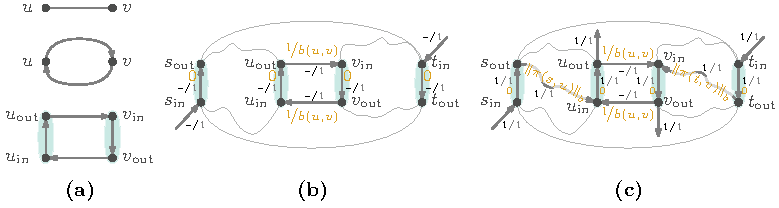
\includegraphics{switchplacement/figures/polynomial_dtp_direct_edges.pdf}
    % 
    \caption[Necessary graph transformation to calculate a polynomial algorithm.]
    {The necessary graph transformations to calculate a~\gls{dtp} in polynomial
    time. (a) The transformation from an undirected graph to a directed graph
    that is bidirected by transforming edge~$\{\vertexa,\vertexb\}$ to two
    directed edges~$(\vertexa,\vertexb), (\vertexb,\vertexa)$. To have a vertex
    disjoint path, each vertex~\vertexa is split into two
    vertices~$\vertexa_{\mathrm{in}},\vertexa_{\mathrm{out}}$ with one
    additional edge~$(\vertexa_{\mathrm{in}},\vertexa_{\mathrm{out}})$. (b) The
    transformed network~$\glssymbol{network}''$ with
    capacities~$\glssymbol{capacity}\equiv 1$ and edges
    costs~$\gamma(\vertexa_{\mathrm{out}},\vertexb_{\mathrm{in}}) =
    \nicefrac{1}{\glssymbol{susceptance}(\vertexa_{\mathrm{out}},\vertexb_{
    \mathrm{in}})}$ for an external edge
    and~$\gamma(\vertexa_{\mathrm{in}},\vertexa_{\mathrm{out}}) = 0$ for a
    vertex internal edge. (c) The resulting minimum-cost flow~\glssymbol{flow}
    for an edge~$\edge_{\min} = (\vertexa,\vertexb)$. }%
    % 
    \label{ch:switching:sec:computing_one_dtp:fig:poly-alg}
    % 
\end{figure}
% 
The previous algorithm computes all~\gls{dtp}{s} between two vertices~\vertexa
and~\vertexb, but has an exponential running time or uses exponential space
dependent on the implementation. In this section, we present a polynomial time
algorithm to calculate the~\gls{dtp}. However, instead of calculating
all~\gls{dtp}{s} between two vertices~\vertexa and~\vertexb this algorithm
computes only one~\gls{dtp}. Thus, it cannot be used for the centrality
measurement. Recall
from~\cref{ch:switching:sec:exploit_structural_characteristics:subsec:dtp} that
a label~$(\bnorm{\fpath{}{\source}{\vertexa}},
\glssymbol{mincapacity}(\fpath{}{\source}{\vertexa}))$ consists of the
susceptance norm---representing the electrical distance---and the minimum
capacity along a path~$\fpath{}{\source}{\vertexa}$. Thus, fixing the edge with
the smallest capacity and calculating a shortest path from that particular edge
to the source and sink vertex using the susceptance norm~$\bnorm{\cdot}$ is
equivalent to the bicriterial shortest path.
% 
%%%%%%%%%%%%%%%%%%%%%%%%%%%%%%%%%% ALGORITHM %%%%%%%%%%%%%%%%%%%%%%%%%%%%%%%%%%%
% \begin{algorithm}[tb!]
%   \SetAlgoLined
%   \SetKwFunction{kwfTodo}{todo}
%   \SetKwFunction{isMarked}{isMarked}
%   \SetKwFunction{kwfUnmark}{unmark}
%   \SetKwFunction{kwfMark}{mark}
%   \SetKwFunction{kwfPush}{push\_back}
%   \SetKwFunction{kwfParent}{parent}
%   \SetKwFunction{kwfDelMin}{delMin}
%   \SetKwFunction{kwfInsert}{insert}
%   \SetKwFunction{kwfSplit}{split}
%   \SetKw{kwfrom}{from}
%   \SetKw{kwto}{to}
%   \SetKw{kwcontinue}{continue}
%   \SetKw{kwfalse}{false}
%   \SetKw{kwtrue}{true}
%   % 
%   \KwData{ A directed graph~$\graph=
%   (\vertices,\edges, \susceptance)$ with transformed edge weights~$\susceptance$,
%   a source~$\source\in\vertices$, and a shortest path tree~$T$ of~$\graph$.}
%   % 
%   \KwResult{Shortest Pairs of Disjoint Paths.}
%   % 
%   % INITIALIZATION %%%%%%%%%%%%%%%%%%%%%%%%%%%%%%%%%%%%%%%%%%%%%%%%%%%%%%%%%%%%
%   $\labels(\vertexa)\coloneq\emptyset; p(\vertexa) \coloneq q(\vertexa) \coloneq
%   \mathrm{NULL};
% \hspace{1em}\forall\vertexa\in\vertices$%
%   \Comment*{\color{KITblack30}Initialization}%
%   \label{alg:initialization_begin}
%   $d(\vertexa) \coloneq \infty\hspace{1em}\forall\vertexa\in\vertices\setminus
%   \{\source\}$\;
%   $d(\source)  \coloneq 0$\;
%   $S \coloneq T$\;
%   % $$\;
%   % 
%   % USING DIJKSTRAS ALGORITHM AND MAINTAINING UNLABELED SUBTREES %%%%%%%%%%%%%%
%   \While(\Comment*[f]{\color{KITblack30}Dijkstra's Algorithm})
%   {$Q\not=\emptyset$}
%   { % while
%     $(d, \vertexb, key) \coloneq Q.\kwfDelMin()$\; 
%     % Splitting S into new Subtrees S'(u) with u unlabled neighbor of v
%     $\{S'(\vertexa)\}_{\vertexa\in
%     N(\vertexb)} \coloneq \kwfSplit(S,\vertexb)$\;
%     % Calculate distances d() and p(), q()
%     \For(\Comment*[f]{\color{KITblack30}Calculate distances and set pointer})
%     {$(\vertexa,\vertexc)\in\edges\setminus T \land \vertexa,\vertexc\in S \land 
%       (\vertexa = \vertexb \lor S'(\vertexa) \not= S'(\vertexc))$}{
%       \If{$d(\vertexb) + \frac{1}{\susceptance(\vertexa,\vertexc)} < d(\vertexc)$}{
%         $d(\vertexc) \coloneq d(\vertexb) + \frac{1}{\susceptance(\vertexa,\vertexc)}$\;
%         $p(\vertexc) \coloneq \vertexa$; $q(\vertexc) \coloneq \vertexb$\;
%         $Q.\kwfInsert(\vertexc,d(\vertexc))$\;
%       }  
%     } % for
%   } % while
%   % 
%   % CONSTRUCTING PATHS %%%%%%%%%%%%%%%%%%%%%%%%%%%%%%%%%%%%%%%%%%%%%%%%%%%%%%%%
%   % Initialization
%   \Comment{\color{KITblack30}Constructing Paths}
%   $\kwfMark(\vertexa) := \kwfalse\hspace{1em}\forall\vertexa\in\vertices$\;
%   $path = \emptyset$\;
%   \While(\Comment*[f]{\color{KITblack30}Constructing Paths Initialization})
%   {$\vertexc\not=\source$}
%   { % while
%     $\vertexc \coloneq \sink$\;
%     $\kwfMark (\vertexa) \coloneq \kwtrue$\;
%     $\vertexc \coloneq q(\vertexc)$
%   }
%   % Backward search
%   \While(\Comment*[f]{\color{KITblack30}Backward search})
%   {$\vertexc\not=\source$}
%   { % while
%     \uIf{$\isMarked(\vertexc)$}{
%       $\kwfMark(\vertexc) \coloneq \kwfalse$\;
%       $path.\kwfPush(p(\vertexc),\vertexc)$\;
%       $\vertexc \coloneq p(\vertexc)$\;
%     } % if
%     \Else{
%       $y \coloneq T.\kwfParent(\vertexc)$\;
%       $path.\kwfPush(y,\vertexc)$\;
%       $\vertexc \coloneq y$\;
%     }
%   }
% %       \Return{$\colorlabels_\forbidden(\vertexb)$}
%   \caption{Shortest Pair of Disjoint Paths~\citep{NET:NET3230140209}}
%   \label{ch:switching:sec:exploit_structural_characteristics:alg:disjoint_paths}
% \end{algorithm}
% 
Assume that one knows an edge~$\edge_{\min}$ on the~\gls{dtp} from~\source
to~\sink with the minimum capacity. We then need to find a
shortest~\source-\sink-path~\pathu via~$\edge_{\min}$, where all edges
of~\pathu\ have capacity at least~$\glssymbol{capacity}(\edge_{\min})$.
Let~$\glssymbol{network}'$ be the network obtained from~\glssymbol{network} when
all edges with capacity smaller than~$\glssymbol{capacity}(\edge_{\min})$ are
removed. Searching for a shortest~\source-\sink-path via~$\edge_{\min}$ is then
equivalent to searching two disjoint paths~$\pathu_1$ and~$\pathu_2$
from~\source and~\sink to the endpoints of~$\edge_{\min}$
in~$\glssymbol{network}'$ such that~$\bnorm{\pathu_1}+\bnorm{\pathu_{2}}$ is
minimum.

These paths can be found by running a minimum-cost flow algorithm in a suitable
graph, which is obtained in the following way. First, we denote the endpoints
of~$\edge_{\min}$ by~\vertexa and~\vertexb, and remove~$\edge_{\min}$. We
replace each undirected edge by directed edges in both directions (bidirected
graph). Finally, each vertex~\vertexc is split into two
vertices~$\vertexc_\mathrm{in}$ and~$\vertexc_\mathrm{out}$, which are joined by
the directed edge $(\vertexc_\mathrm{in},\vertexc_\mathrm{out})$. We call these
edges \emph{internal}. The incoming and outgoing edges of~\vertexc are then
placed at~$\vertexc_\mathrm{in}$ and~$\vertexc_\mathrm{out}$, respectively. All
edges of the resulting graph get a capacity of~$1$. The cost of the internal
edges is set to~$0$. All other edges correspond to an edge~$\edge$ in the input
network, and we set their costs to
$\nicefrac{1}{\glssymbol{susceptance}(\edge)}$. The
vertices~$\source_\mathrm{out}$ and~$\sink_\mathrm{out}$ produce one unit of
flow each, while~$\vertexa_\mathrm{in}$ and~$\vertexb_\mathrm{in}$ consume one
unit each. We call the resulting network~$\glssymbol{network}''$.

Let~$\glssymbol{flow}$ be a minimum-cost flow from~\vertexa to~\vertexb with
flow value~$2$. We can decompose~$\glssymbol{flow}$ into two unit flows
from~$\source_\mathrm{in}$ and~$\sink_\mathrm{in}$, which correspond to disjoint
paths~$\pathu_1$ and~$\pathu_2$ from~\source and~\sink to the endpoints~\vertexa
and~\vertexb (\ie, endpoints of the removed edge~$\edge_{\min}$).
% 
\begin{lemma}
    The shortest~\source-\sink-path~\pathu via~$\edge_{\min}$
    in~$\glssymbol{network}_{\glssymbol{capacity}(\edge_{\min})}$ has
    susceptance
    norm~$\bnorm{\pathu}=\flowcost(\glssymbol{flow})+\bnorm{\edge_{\min}}$. If
    the edge on~\pathu with the minimum capacity is known, \pathu can be
    computed in polynomial time.
    % 
    \label{ch:switching:sec:exploit_structural_characteristics:lem:min_cost_flow_dtp}
\end{lemma}
% 
\begin{proof}
    Constructing $\glssymbol{network}''$ as described above and computing the minimum-cost
    flow~$\glssymbol{flow}$ is possible in polynomial time. The
    flow~\glssymbol{flow} can be
    decomposed into two unit flows, \eg, by running a depth-first search. The
    edge capacities of~$1$ ensure that these two flows follow two edge-disjoint
    paths. Since each vertex of~$\glssymbol{network}''$ has only one incoming or one
    outgoing edge, these paths are vertex-disjoint as well. Further, they
    correspond to two paths~$\pathu_1$ and~$\pathu_2$ in~$\glssymbol{network}'$,
    where~$\pathu_1$ connects~\source with an endpoint of~$\edge_{\min}$
    and~$\pathu_2$ connects~\sink with the other endpoint of~$\edge_{\min}$.
    Together with~$\edge_{\min}$ we hence obtain an
    \source-\sink-path~\paths via~$\edge_{\min}$ 
    with~$\bnorm{\pathu}=\flowcost(\glssymbol{flow})+\bnorm{\edge_{\min}}$. The last
    property follows immediately from the definition of the costs
    in~$\glssymbol{network}''$. As~$\glssymbol{flow}$ has minimum cost, the
    constructed path~\pathu has
    minimum susceptance norm among all~\source-\sink-paths
    via~$\bnorm{\pathu}=\flowcost(\glssymbol{flow})+\bnorm{\edge_{\min}}$
    in~$\glssymbol{network}'$.
\end{proof}

Since we assumed that~$\edge_{\min}$ was an edge with minimum capacity on
a~\gls{dtp} between~\source and~\sink, the path~\pathu is a~\gls{dtp}.
However, $\edge_{\min}$ is unknown. We therefore repeat this procedure for each
edge in the network and pick the path with the smallest angle difference.
\cref{ch:switching:sec:exploit_structural_characteristics:lem:min_cost_flow_dtp}
then guarantees that this results in a~\gls{dtp}.
% 
%%%%%%%%%%%%%%%%%%%%%%%%%%%%%%%%%%%%%%%%%%%%%%%%%%%%%%%%%%%%%%%%%%%%%%%%%%%%%%%
%%%%%%%%%%%%%%%%%%%%%%%%%%%%%%%%%%%%%%%%%%%%%%%%%%%%%%%%%%%%%%%%%%%%%%%%%%%%%%%
\section{Approximation Algorithm on Cacti}
\label{ch:switching:sec:approximation_algorithm_on_cacti}
%%%%%%%%%%%%%%%%%%%%%%%%%%%%%%%%%%%%%%%%%%%%%%%%%%%%%%%%%%%%%%%%%%%%%%%%%%%%%%%
%
%%%%%%%%%%%%%%%%%%%%%%%%%%%%%%%%%% ALGORITHM %%%%%%%%%%%%%%%%%%%%%%%%%%%%%%%%%%%
\begin{algorithm}[tb!]
\SetAlgoLined
  % 
  \KwData{A network~$\glssymbol{network} = 
  (\glssymbol{graph},\glssymbol{generators},\glssymbol{consumers},\glssymbol{capacity},\glssymbol{susceptance})$.}
  % 
  \KwResult{ $\opt_{\gls{mpfp}}(\glssymbol{network}-\glssymbol{switched})$, and
  switched edges~$\glssymbol{switched}$. }
  % 
  $\glssymbol{switched} = \emptyset$\;
  $\glssymbol{cycles}$ = \algodfs($\glssymbol{network}$)\;
  % 
  \For{$\glssymbol{cycle}\in\glssymbol{cycles}$}{%
      $\glssymbol{switched} = \glssymbol{switched}
      \cup
      \{\argmin_{\forall\edge\in\glssymbol{cycle}}(\glssymbol{capacity}(\edge))\}$\;
  }
  % 
  \Return{$\left(\opt_{\gls{mfp}}(\glssymbol{network}-\glssymbol{switched}),\glssymbol{switched}\right)$}\;
  \caption{Factor~$2$-Approximation Algorithm for Cacti}
  \label{ch:switching:sec:approximation_algorithm_on_cacti:alg:factor_2_approximation}
\end{algorithm}
%
% 
\textcite{Leh14} showed that the bounded~\gls{mtsfp} on cacti is~\NP-hard by
using a reduction from subset sum. Subset sum is weakly~\NP-hard and a fully
polynomial-time approximation scheme (\gls{fptas})
exists~\parencite{krps-fptasSubsetSum-2003}.
% 
In this section, we present an approximation algorithm for~\gls{mtsfp} on
cacti with approximation factor 2. Recall
from~\cref{ch:switching:sec:network_modeling} that it is always possible to
transform a bounded~\gls{mtsfp} into an unbounded~\gls{mtsfp}
(\cref{lem:bounded_unbounded_mtsf_transformation}).

In the following, we assume that our underlying graph~\glssymbol{graph}
of~\glssymbol{network} is a cactus. Unlike
in~\cref{ch:switching:sec:exploit_structural_characteristics} we allow multiple
generators and consumers.
% 
The basic idea for our algorithm
(\cref{ch:switching:sec:approximation_algorithm_on_cacti:alg:factor_2_approximation})
is to remove from each cycle the edge with the smallest capacity. Since we
presume that~\glssymbol{network} is a cactus, cycles are independent concerning
the voltage angle difference, since they do not share an edge. Cycle detection
can be done via a~\acrlong{dfs}~(\gls{dfs})
in~$\bigO(\fmagnitude{\glssymbol{vertices}})$ time,
where~$\fmagnitude{\glssymbol{vertices}}$ is the number of vertices. Finding
the edge with minimum capacity in each cycle is done during the~\gls{dfs}.
% 
% 
Note that the remaining structure is a tree that is equivalent to
a~\acrlong{maxst} (\gls{maxst}). The running time of~\gls{maxst} is in
general~$\bigO(\fmagnitude{\glssymbol{edges}}~\alpha(\fmagnitude{\glssymbol{edges}},
\fmagnitude{\glssymbol{vertices}}))$~\parencite{Cha00}, where~$\alpha$ is the
inverse of the Ackermann function (\ie, $\alpha$ grows very slowly). Note
that~\gls{maxst} on cacti runs also in~$\bigO
(\fmagnitude{\glssymbol{vertices}})$ time.
% 
The maximum flow on trees can be realized
in~$\bigO(\fmagnitude{\glssymbol{vertices}})$ time by using the pseudoflow
algorithm~\parencite{Hoc08}. Thus, the algorithm runs
in~$\bigO(\fmagnitude{\glssymbol{vertices}})$ time.
%
%%%%%%%%%%%%%%%%%%%%%%%%%%%%%%%%%%%% LEMMA %%%%%%%%%%%%%%%%%%%%%%%%%%%%%%%%%%%%
\begin{lemma}
    Let~$\glssymbol{network}=
    (\glssymbol{graph},\glssymbol{generators},\glssymbol{consumers},\glssymbol{capacity},\glssymbol{susceptance})$
    be a power grid and let~\glssymbol{switched} be the set
    $\argmin_{\forall\edge\in\glssymbol{cycle}}$ $\glssymbol{capacity}(\edge)$
    of switched edges for all cycles~$\glssymbol{cycle}\in\glssymbol{cycles}$.
    Then there exist a feasible electrical flow~$\glssymbol{flow}'$
    on~$\glssymbol{network}-\glssymbol{switched}$ such
    that~$\glssymbol{flowvalue}(\glssymbol{flow}')=
    \nicefrac{1}{2}~\opt_{\gls{mf}}(\glssymbol{network})$.% 
    %
    \label{ch:switching:sec:approximation_algorithm_on_cacti:lem:half_flow}
\end{lemma}
%
\begin{proof}
Let~$\glssymbol{flow}^\star$ be a~\gls{mf} with value~$\opt_{\gls{mfp}}$
on~\glssymbol{network}. By reducing the flow on each edge by one half
(see~\cref{ch:switching:sec:approximation_algorithm_on_cacti:eq:half_flow}), we
get a flow~\glssymbol{flow} on~\glssymbol{network} with a value of~$\nicefrac{1}
{2}~\opt_{\gls{mf}}$.
Applying~\cref{ch:switching:sec:approximation_algorithm_on_cacti:alg:factor_2_approximation}
% 
returns a set of switched edges~$\glssymbol{switched} =
\bigcup_{\glssymbol{cycle}\in\glssymbol{cycles}}
\argmin_{\forall\edge\in\glssymbol{cycle}}\glssymbol{capacity} (\edge)$.
% 
We decompose each cycle~$\glssymbol{cycle}\in\glssymbol{cycles}$ into an
edge~$\edge_{\min}$ having the smallest capacity on the cycle~\glssymbol{cycle}
(\cref{ch:switching:sec:approximation_algorithm_on_cacti:eq:capacity_flow_behavior})
and into the remaining part denoted as path~$\pathu$. Since the flow
on~$\edge_{\min}$ is~$\nicefrac{1}{2}\glssymbol{flow}^\star(\edge_{\min})$ it
can be rerouted on the remaining part~$\pathu$ of~\glssymbol{cycle}
(\cref{ch:switching:sec:approximation_algorithm_on_cacti:eq:rerouted_flow}). We
denote the rerouted flow by~$\glssymbol{flow}'$. For any~$\edge\in\pathu$ we
have
%
%%%%%%%%%%%%%%%%%%%%%%%%%%%%%%%%%%% EQUATION %%%%%%%%%%%%%%%%%%%%%%%%%%%%%%%%%%
\begin{align}
  \fmagnitude{\glssymbol{flow}(\edge)} = 
  \fmagnitude{\nicefrac{1}{2}~\glssymbol{flow}^\star(\edge)}&
  \leq\nicefrac{1}{2}~\glssymbol{capacity}(\edge),& 
  %
  \label{ch:switching:sec:approximation_algorithm_on_cacti:eq:half_flow}\\
  %%%%%%%%%%%%%%%%%%%%%%%%%%%%%%%%%%%%%%%%%%%%%%
  %
  %%%%%%%%%%%%%%%%%%%%%%%%%%%%%%%%%%%%%%%%%%%%%%
  \fmagnitude{\glssymbol{flow}(\edge_{\min})}
  \leq\nicefrac{1}{2}~\glssymbol{capacity}(\edge_{\min}) &\leq
  \nicefrac{1}{2}~\glssymbol{capacity}(\edge),&
  %
  \label{ch:switching:sec:approximation_algorithm_on_cacti:eq:capacity_flow_behavior} 
  \\
  %%%%%%%%%%%%%%%%%%%%%%%%%%%%%%%%%%%%%%%%%%%%%%
  \fmagnitude{\glssymbol{flow}'(\edge)} =
  \fmagnitude{\glssymbol{flow}(\edge_{\min}) + 
  \glssymbol{flow}(\edge)}&\leq\glssymbol{capacity}(\edge).&
  % 
  \label{ch:switching:sec:approximation_algorithm_on_cacti:eq:rerouted_flow}
\end{align}
% 
\end{proof}
%
% 
\begingroup
% \tikzset{font={\fontsize{8pt}{12}\selectfont}}
\begin{center}%
    \begin{figure}[t!]%
        \begin{subfigure}[b]{.498\textwidth}%
            \centering%
            \resizebox {\columnwidth} {!} {%
                \includegraphics{switchplacement/plots/plot-SwitchingBetweenness_nesta_case189_edin-dtpbc-mpf-cutY-StandAlone.pdf}%
            }%
            \label{ch:switching:sec:evaluation:plot:a:SwitchingBetweenness_nesta_case189_edin_dtpbc_mpf_cutY}%
            \caption{}%
        \end{subfigure}%
        \hfill%
        \begin{subfigure}[b]{.498\textwidth}%
            \centering%
            \resizebox {\columnwidth} {!} {%
                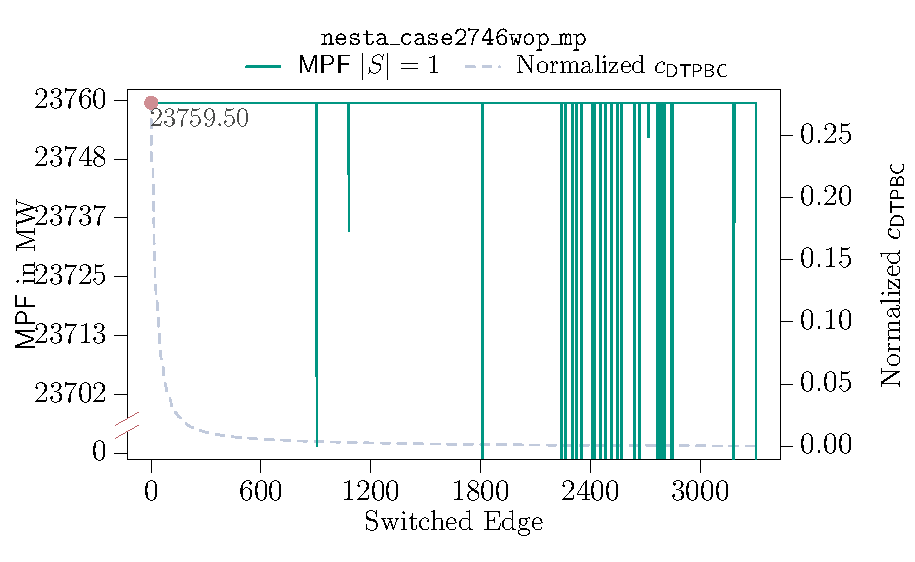
\includegraphics{switchplacement/plots/plot-SwitchingBetweenness_nesta_case2746wop_mp-dtpbc-mpf-cutY-StandAlone.pdf}%
            }%
            \label{ch:switching:sec:evaluation:plot:a:SwitchingBetweenness_nesta_case2746sp_mp_dtpbc_mpf_cutY}%
            \caption{}%
        \end{subfigure}%
        % 
    
        % 
        \hspace{-0.3cm}
        \begin{subfigure}[b]{.498\textwidth}%
            \centering%
            \resizebox {.865\columnwidth} {!} {
                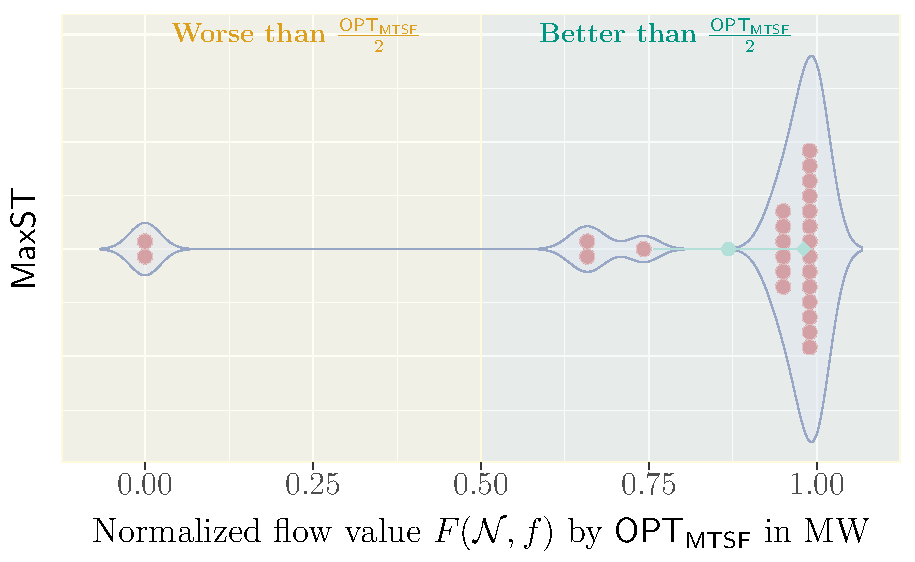
\includegraphics{switchplacement/plots/plot-maxst-vs-mtsf-violin-swarm-StandAlone.pdf}
                \label{ch:switching:sec:evaluation:plot:twoApproximation_violin}%
            }
            \caption{}%
        \end{subfigure}%
        % 
        \hfill%
        % 
        \begin{subfigure}[b]{.498\textwidth}%
            \centering%
            \resizebox {\columnwidth} {!} {
                \includegraphics{switchplacement/plots/plot_dtp_betweenness_centrality_all_quantiles-StandAlone.pdf}
                % 
                \label{ch:switching:sec:evaluation:plot:dtp_betweenness_centrality_all_quantiles}%
            }%
            \caption{}%
            \label{ch:switching:sec:evaluation:fig:simulations:dtp}
        \end{subfigure}%
        % 
        %
        \caption[Simulation results for switching.]{Simulation evaluation using
        the data
        from~\cref{ch:switching:sec:evaluation:tbl:MTSF_MPF_PF_MF_long}~for~(c)
        and aggregating the results
        from~\crefrange{fig:Switching_Betweenness_Centrality_Plot_Cut_Y_3_to_24}
        {fig:Switching_Betweenness_Centrality_Plot_Cut_Y_162_to_3012} into (d)
        including (a) and (b). (a) and (b) show the
        \texttt{nesta\_case189\_edin} and \texttt{2746wop\_mp}, respectively,
        with the gray dashed line being the centrality of the edges (x-axis) and
        the green line the~\gls{mpf}~(y-axis). (c)~The~$2$-approximation on
        cacti using~\gls{maxst} is tested on arbitrary graphs. The global
        optimum~$\opt_{\gls{maxst}}$ is reached at~$1$ and the proven factor for
        cacti is at~$\nicefrac{1}{2}$. The green left (with range) and right
        point show the mean and median, respectively. (d)~The aggregated data
        are normalized with regards to the edges and~\gls{mpf}
        using~$\fmagnitude{\glssymbol{edges}}$ and the~\gls{mpf} of each of the
        network. The edges are ranked from highest to lowest~$c_{\sbc}$. The
        quantiles show that 32~\% of the test cases give worse results than the
        green line while switching an edge with low centrality.}%
        % 
        \label{ch:switching:sec:evaluation:fig:simulations}
    \end{figure}
\end{center}
\endgroup
% 
Recall that~$\opt_{\gls{mfp}}$ is an upper bound for~$\opt_{\gls{mtsfp}}$ and
that~\gls{mfp} and~\gls{mtsfp} are equal on trees. Thus,
from~\cref{ch:switching:sec:approximation_algorithm_on_cacti:lem:half_flow}
follows~\cref{ch:switching:sec:approximation_algorithm_on_cacti:thm:cacti_2_approximation}. %the next
% 
% 
%%%%%%%%%%%%%%%%%%%%%%%%%%%%%%%%%%%% THEOREM %%%%%%%%%%%%%%%%%%%%%%%%%%%%%%%%%%
\begin{theorem}
\label{ch:switching:sec:approximation_algorithm_on_cacti:thm:cacti_2_approximation}
% 
\cref{ch:switching:sec:approximation_algorithm_on_cacti:alg:factor_2_approximation}
is a factor~$2$-approximation algorithm for the~\gls{mfp} and~\gls{mtsfp} problem
on cacti.
\end{theorem}
% 
Note that an approximation ratio of~$\nicefrac{1}{2}$ does not provide a good
guarantee in the worst case. However, compared to other heuristics it gives
guarantees and can be used as an initial step for heuristics.
% 
% \clearpage
%%%%%%%%%%%%%%%%%%%%%%%%%%%%%%%%%%%%%%%%%%%%%%%%%%%%%%%%%%%%%%%%%%%%%%%%%%%%%%%
\section{Simulations}  
\label{ch:switching:sec:evaluation}
%%%%%%%%%%%%%%%%%%%%%%%%%%%%%%%%%%%%%%%%%%%%%%%%%%%%%%%%%%%%%%%%%%%%%%%%%%%%%%%
% 
We simulated\footnote{\href{https://i11www.iti.kit.edu/projects/mtsf/index}{https://i11www.iti.kit.edu/projects/mtsf/index}} 
% 
our~\gls{dtp}~betweenness centrality and 2-approximation algorithms for
penrose-minor-free graphs and cacti, respectively, on arbitrary graphs.
% 
By arbitrary graph we mean the~\gls{nesta} benchmark sets~\parencite{Cof14b},
which are based on the~\gls{ieee} benchmark
% 
sets~\parencite{online:IEEEtestData,Zimmerman2011a,4075418,Bil70,online:TheUniversityOfEdinburgh:SchoolOfMathematics:PowerSystemsTestCaseArchive,crow2015computational,Dem77,Gra03,780914,
Jos16,6120344,5589973,4113721,Woo13} and 
incorporate 
% 
realistic data such as thermal line limits. Note that we run our simulations on
arbitrary power grids, since there are not a lot of benchmark sets presenting
cacti namely \nestacase{3}, \texttt{4\_gs}, and~\texttt{9\_wscc} 
% 
% 
or~\source-\sink-networks available.
% 
%
Recall from~\cref{ch:switching:sec:model} that we have a disjoint set of
generators and consumers. This theoretical assumption cannot be found in any
benchmark set and realistic power grid. Thus, we have to modify the data in such
a way that we still provide a realistic benchmark set and comply with the
assumptions to avoid infinite generator production at buses having both
generators and consumers
(see~\cref{ch:switching:sec:model:eq:unlimited_generation_constraints,ch:switching:sec:model:eq:unlimited_demand_constraint}).
In addition, we only allow to consume a real power demand~$p_d$ at a real power
generator (see bus data's column three in the~\gls{ieee} Common Data
Format~\parencite{4075293}). All other consumers have an infinite maximum demand
(\cref{ch:switching:sec:model:eq:demand_constraint}). The results for the
problems in~\cref{ch:switching:sec:model} are shown
in~\cref{ch:switching:sec:evaluation:tbl:MTSF_MPF_PF_MF_long}.

For the 2-approximation, we use~\gls{maxst}
(\cref{ch:switching:sec:approximation_algorithm_on_cacti}) on different
benchmark data sets and compare the results with the~\gls{milp}
from~\cref{ch:switching:sec:model}. The algorithm~\gls{maxst} gives very good
results even though operating on arbitrary graphs
(see~\cref{ch:switching:sec:evaluation:tbl:MTSF_MPF_PF_MF_long}). Nearly
all---meaning~$93~\%$---of the results are better than the approximation factor
and~$82~\%$ are at most~$7~\%$ from the optimum value~$\opt_{\gls{mtsfp}}$
(see~\cref{ch:switching:sec:evaluation:fig:simulations}\screen{c}). Note
that~$36~\%$ of the results even reach the optimal value (cases equal
to~$\opt_{\gls{mtsfp}}$ have gray markers
in~\cref{ch:switching:sec:evaluation:tbl:MTSF_MPF_PF_MF_long}). Thus, the
expected quality on arbitrary graphs is much better than the proven
approximation ratio of~$2$ on cacti
(\cref{ch:switching:sec:approximation_algorithm_on_cacti}). There are two cases
worse than the approximation factor, because there is no feasible power flow for
the resulting networks~$\glssymbol{network}-\gls{switched}_{\gls{maxst}}$. There
are three cases in which the number of switched lines in the $2$-approximation
is greater than~$\opt_{\gls{mtsfp}}$. %Note that we do not optimize the number of
%switches.

The~\gls{dtp} is exact for~\source-\sink-penrose-minor-free graphs. There is no
benchmark case providing this structure. However, since the~\gls{dtp} represents
a distance measure, which marks interesting paths for switching, we introduced
the~\gls{dtp}-betweenness centrality
in~\cref{ch:switching:sec:exploit_structural_characteristics:def:dtp_betweenness_centrality}.
To estimate the relation of the power flow and the different edges having
different centrality values~$c_\sbc$ for the different benchmark cases with
different assorted characteristics, we calculated the~\gls{mpf} for the network
after removing a single edge~\edge with centrality~$c_\sbc(\edge)$ from the
network and decreasingly order the normalized edges by the centrality. Note that
we normalized the~\gls{mpf} and edge index by the network's~$\opt_{\gls{mpfp}}$
value and~$\fmagnitude{\gls{edges}}$, respectively. The normalization is
necessary to aggregate all cases
from~\crefrange{fig:Switching_Betweenness_Centrality_Plot_Cut_Y_3_to_24}
{fig:Switching_Betweenness_Centrality_Plot_Cut_Y_162_to_3012} into one plot.
The~$32~\%$ and~$35~\%$ quantiles
in~\cref{ch:switching:sec:evaluation:fig:simulations}\screen{d} show cut points
where the~\gls{mpf} decreases while switching an edge. These quantiles show
that~$32~\%$ of the test cases at low centrality result in worse results than
the plotted line. This effect happens mainly with edges having a small~$c_\sbc$
(\ie, the normalized edge index is close to~$1$). For the~$35~\%$ quantile there
are only deflections at edges with low centrality. Note, that the line at zero
represents~\nestacase{57}, \nestacase{2383}, and~\nestacase{3012}, where
switching of an edge leads to a network with no feasible~\gls{mpf}. Note that
deflection at edges with low centrality motivates the algorithm also
for~\gls{rop}, since edges with low centrality are more essential for the power
grid to get into a stable operation and should be considered first.
%
\begin{landscape}
    \begin{table}
        \centering
        \caption[Switching Results using the~\gls{nesta} Benchmark Sets.]{
        The~\gls{pf}, \gls{mpf}, \gls{mtsf} and~\gls{ots} models
        from~\cref{ch:switching:sec:model} are evaluated on the~\gls{nesta}
        benchmark sets~\parencite{Cof14b}. The
        parameters~$\fmagnitude{\glssymbol{vertices}}$, $
        \fmagnitude{\glssymbol{edges}}$, 
        and~$\fmagnitude{\glssymbol{switched}_{\glssymbol{problems}}}$ represent
        the number of vertices, edges and switched edges for a
        problem~$\glssymbol{problems}$, respectively, and the optimal solutions
        are given in~$\opt_{\glssymbol{problems}}$. Since~\gls{otsp}
        minimizes the cost, the flow value~$\flowvalue_{\gls{otsp}}$ is
        shown, too. The maximum possible generation is given in the last column
        (marked~\myhl{KITred15}{red} if it is larger than
        the~$\opt_{\gls{mfp}}$). The~\myhl{KITyellow15}{yellow} rows mark
        the interesting cases where~$\opt_{\gls{mpfp}}$ is smaller than
        the~$\opt_{\gls{mtsfp}}$. }
        %     
        %     
        %      However, the
        %     five cases in which the~$\opt_\mtsf$ is smaller than the~$\opt_\mf$ are
        %     marked~\myhl{KITblue15}{blue}. The cases in which the~$\opt_\maxst$
        %     (see~\cref{ch:switching:sec:approximation_algorithm_on_cacti})
        %     and~$\opt_\mpf$ are equal to~$\opt_\mtsf$ are
        %     marked~\myhl{KITblack!10}{gray}. In addition, there are three cases in
        %     which the number of switched lines in the~$\switched_\maxst$ is greater
        %     than in the~$\switched_\mtsf$ shown as~\myhl{KITgreen15}{green}. }
        % 
            \label{ch:switching:sec:evaluation:tbl:MTSF_MPF_PF_MF_long}
        % latex table generated in R 3.2.2 by xtable 1.8-0 package
% Fri Jan 26 22:50:42 2018
% \small
\footnotesize
\setlength{\tabcolsep}{4pt}
% \setlength\minrowclearance{3pt}
\begin{tabular}{lrrrrrrrrrrrrr}
  \toprule
  NESTA Case 
  &\hspace{-3mm} $\fmagnitude{\glssymbol{vertices}}$ 
  &\hspace{-3mm} $\fmagnitude{\glssymbol{edges}}$
  &\hspace{-3mm} $\fmagnitude{\glssymbol{switched}_{\gls{mtsfp}}}$ 
  &\hspace{-3mm} $\fmagnitude{\glssymbol{switched}_{\gls{otsp}}}$ 
  &\hspace{-3mm} $\fmagnitude{\glssymbol{switched}_{\gls{maxst}}}$ 
  &\hspace{-3mm} $\opt_{\gls{otsp}}$ in \$ 
  &\hspace{-3mm} $\flowvalue_{\gls{otsp}}$ 
  &\hspace{-3mm} $\opt_{\gls{pf}}$ 
  &\hspace{-3mm} $\opt_{\gls{mpfp}}$ 
  &\hspace{-3mm} $\opt_{\gls{mtsfp}}$ 
  &\hspace{-3mm} $\opt_{\gls{maxst}}$ 
  &\hspace{-3mm} $\opt_{\gls{mfp}}$ 
  &\hspace{-3mm} $\max$ Gen \\
 \midrule
\rowcolor{KITyellow15}\tablecase{nestacase3lmbd} &   3 &   3 & 1 & 1 & 1 &       5\,638.97 & 315 &      315.00 &      353.53 &  4\,000.00 & \cellcolor{KITblack!10} 4\,000.00 &  4\,000.00 &  4\,000.00 \\ 
  \tablecase{nestacase4gs} &   4 &   4 & \cellcolor{KITgreen15}0 & 1 & \cellcolor{KITgreen15}1 &           109.99 & 500 &      500.00 & \cellcolor{KITblack!10}     969.00 &      969.00 &      719.00 &      969.00 & \cellcolor{KITred15} 1\,639.00 \\ 
  \tablecase{nestacase5pjm} &   5 &   6 & \cellcolor{KITgreen15}0 & 1 & \cellcolor{KITgreen15}3 &      14\,991.30 & 1000 &  1\,000.00 & \cellcolor{KITblack!10} 1\,448.39 & \cellcolor{KITcyanblue15} 1\,448.39 &  1\,356.00 & \cellcolor{KITcyanblue15} 1\,530.00 &  1\,530.00 \\ 
  \tablecase{nestacase6c} &   6 &   7 & 4 & 1 & 4 &            22.77 & 107.5 &      107.50 & \cellcolor{KITblack!10}     370.00 &      370.00 &      248.00 &      370.00 & \cellcolor{KITred15} 1\,002.00 \\ 
  \rowcolor{KITyellow15}\tablecase{nestacase6ww} &   6 &  11 & 6 & 6 & 6 &       3\,046.41 & 210 &      210.00 &      332.80 & \cellcolor{KITcyanblue15}     360.00 & \cellcolor{KITblack!10}     360.00 & \cellcolor{KITcyanblue15}     470.00 & \cellcolor{KITred15}     530.00 \\ 
  \tablecase{nestacase9wscc} &   9 &   9 & 6 & 0 & 2 &       5\,216.03 & 315 &      315.00 & \cellcolor{KITblack!10}     770.00 &      770.00 & \cellcolor{KITblack!10}     770.00 &      770.00 & \cellcolor{KITred15}     820.00 \\ 
  \tablecase{nestacase14ieee} &  14 &  20 & 15 & 7 & 10 &           231.41 & 259 &      259.00 & \cellcolor{KITblack!10}     425.00 &      425.00 & \cellcolor{KITblack!10}     425.00 &      425.00 &      425.00 \\ 
  \tablecase{nestacase24ieeerts} &  24 &  38 & 28 & 10 & 18 &      61\,001.20 & 2850 &  2\,850.00 & \cellcolor{KITblack!10} 3\,405.00 &  3\,405.00 & \cellcolor{KITblack!10} 3\,405.00 &  3\,405.00 &  3\,405.00 \\ 
  \rowcolor{KITyellow15}\tablecase{nestacase29edin} &  29 &  99 & \cellcolor{KITgreen15}55 & 54 & \cellcolor{KITgreen15}79 &      29\,669.40 & 56325.9 & 56\,325.90 & 81\,597.50 & \cellcolor{KITcyanblue15}81\,603.40 & 76\,158.80 & \cellcolor{KITcyanblue15}82\,384.80 & 82\,384.80 \\ 
  \tablecase{nestacase30as} &  30 &  41 & 32 & 10 & 15 &           767.60 & 283.4 &      283.40 & \cellcolor{KITblack!10}     435.00 &      435.00 & \cellcolor{KITblack!10}     435.00 &      435.00 &      435.00 \\ 
  \tablecase{nestacase30fsr} &  30 &  41 & 30 & 14 & 15 &           565.21 & 189.2 &      189.20 & \cellcolor{KITblack!10}     335.00 &      335.00 &      322.20 &      335.00 &      335.00 \\ 
  \tablecase{nestacase30ieee} &  30 &  41 & 34 & 12 & 19 &           152.67 & 283.4 &      283.40 & \cellcolor{KITblack!10}     390.00 &      390.00 &      252.00 &      390.00 & \cellcolor{KITred15}     884.00 \\ 
  \tablecase{nestacase39epri} &  39 &  46 & 35 & 7 & 17 &      95\,578.30 & 6254.23 &  6\,254.23 & \cellcolor{KITblack!10} 7\,227.00 &  7\,227.00 & \cellcolor{KITblack!10} 7\,227.00 &  7\,227.00 & \cellcolor{KITred15} 7\,367.00 \\ 
  \tablecase{nestacase57ieee} &  57 &  80 & 75 & 25 & 40 &       1\,125.14 & 1250.8 &  1\,250.80 & \cellcolor{KITblack!10} 1\,377.00 &  1\,377.00 & \cellcolor{KITblack!10} 1\,377.00 &  1\,377.00 &  1\,377.00 \\ 
  \tablecase{nestacase73ieeerts} &  73 & 120 & 87 & 34 & 56 &     183\,004.00 & 8550 &  8\,550.00 & \cellcolor{KITblack!10}10\,215.00 & 10\,215.00 & \cellcolor{KITblack!10}10\,215.00 & 10\,215.00 & 10\,215.00 \\ 
  \tablecase{nestacase89pegase} &  89 & 210 & 145 & 70 & 142 &       5\,733.37 & 5733.37 &  5\,733.37 & \cellcolor{KITblack!10} 9\,921.23 &  9\,921.23 &  9\,718.23 &  9\,921.23 &  9\,921.23 \\ 
  \tablecase{nestacase118ieee} & 118 & 186 & 150 & --- & 92 & --- & --- &  4\,242.00 & \cellcolor{KITblack!10} 7\,119.00 & \cellcolor{KITcyanblue15} 7\,119.00 &  6\,830.00 & \cellcolor{KITcyanblue15} 7\,134.00 &  7\,134.00 \\ 
  \tablecase{nestacase162ieeedtc} & 162 & 284 & 269 & 77 & 154 &       3\,904.81 & 7239.06 &  7\,239.06 & \cellcolor{KITblack!10} 8\,296.00 &  8\,296.00 &  7\,931.00 &  8\,296.00 & \cellcolor{KITred15} 9\,685.00 \\ 
  \tablecase{nestacase189edin} & 189 & 206 & 71 & 62 & 62 &           783.95 & 1367.83 &  1\,367.83 & \cellcolor{KITblack!10} 2\,987.00 &  2\,987.00 & \cellcolor{KITblack!10} 2\,987.00 &  2\,987.00 & \cellcolor{KITred15} 3\,012.00 \\ 
  \tablecase{nestacase300ieee} & 300 & 411 & 290 & --- & 185 & --- & --- & 23\,527.20 & \cellcolor{KITblack!10}31\,568.00 & \cellcolor{KITcyanblue15}31\,568.00 & 30\,504.00 & \cellcolor{KITcyanblue15}31\,735.00 & \cellcolor{KITred15}32\,492.00 \\ 
  \tablecase{nestacase2736spmp} & 2736 & 3269 & 2518 & 545 & 1307 &     991\,228.00 & 18074.5 & 18\,074.50 & \cellcolor{KITblack!10}20\,246.70 & 20\,246.70 & 20\,010.70 & 20\,246.70 & 20\,246.70 \\ 
  \tablecase{nestacase2737sopmp} & 2737 & 3269 & 2536 & 630 & 1305 &     621\,780.00 & 11267.2 & 11\,267.20 & \cellcolor{KITblack!10}14\,677.90 & 14\,677.90 & 14\,537.20 & 14\,677.90 & 14\,677.90 \\ 
  \tablecase{nestacase2746wopmp} & 2746 & 3307 & 2547 & 649 & 1349 &     861\,568.00 & 18960 & 18\,960.00 & \cellcolor{KITblack!10}23\,759.50 & 23\,759.50 & --- & 23\,759.50 & 23\,759.50 \\ 
  \tablecase{nestacase2746wpmp} & 2746 & 3279 & 2487 & 594 & 1318 & 1\,261\,620.00 & 24873 & 24\,873.00 & \cellcolor{KITblack!10}27\,618.70 & 27\,618.70 & --- & 27\,618.70 & 27\,618.70 \\ 
  \tablecase{nestacase3120spmp} & 3120 & 3693 & 2793 & --- & 1513 & --- & --- & 21\,181.50 & \cellcolor{KITblack!10}25\,406.00 & 25\,406.00 & 24\,856.50 & 25\,406.00 & 25\,406.00 \\ 
   \bottomrule
\end{tabular}% table
    \end{table}
\end{landscape}
%
% 
%%%%%%%%%%%%%%%%%%%%%%%%%%%%%%%%%%%%%%%%%%%%%%%%%%%%%%%%%%%%%%%%%%%%%%%%%%%%%%%
%%%%%%%%%%%%%%%%%%%%%%%%%%%%%%%%%%%%%%%%%%%%%%%%%%%%%%%%%%%%%%%%%%%%%%%%%%%%%%%
\section{Conclusion}    
\label{ch:switching:sec:conclusion}
%%%%%%%%%%%%%%%%%%%%%%%%%%%%%%%%%%%%%%%%%%%%%%%%%%%%%%%%%%%%%%%%%%%%%%%%%%%%%%%
% 
This paper is the first to provide algorithms with provable guarantees
for~\gls{mtsfp} on certain graph structures and shrinks the gap between theory
and practice. In addition, it provides an extensive theoretical analysis of
the~\gls{mtsfp}, builds connections to related problems and shows how to
simplify the network including the transformations from a bounded to an 
unbounded~\gls{mtsfp}, and the equivalence of~\gls{otsp} and~\gls{mtsfp}. We
introduce an exact algorithm for networks with one generator and one consumer
for certain network structures and show when it becomes~\NP-hard
on~\source-\sink-networks. On that base, we define a new centrality measure
based on~\acrlong{dtp}{s} (\gls{dtp}{s}) representing
% 
the~\source-\sink-path with the smallest voltage angle difference. For multiple
generators and sinks in the network, we give a~$2$-approximation for cacti. At
the end, the complementing evaluation rounds off the theoretical results. The
simulations show very good results on the~\gls{nesta} benchmark set with
arbitrary graph structures, \ie, the results are in nearly all cases either
optimal or very close to the optimum.

However, there are many open problems. It is unknown if the reachability test
can be done in polynomial time and, if not, if there is still a polynomial time
algorithm for~\gls{dtp} (see discussion
in~\cref{ch:switching:sec:exploit_structural_characteristics:subsec:reachibility_test}).
Another open question is if there is a~\gls{ptas} on cacti. The current
idea is a rounding based algorithm. There are many other open problems such as
the complexity and the existence of algorithms while fixing a set of edges as
% 
non-switchable (motivated by~\gls{tnep}), as well as minimizing or
constraining the number of switches. In addition, we used a linearization of
the~\gls{ac}-model denoted by~\gls{dc}-model. Though, we could not
easily transfer our results directly to~\gls{ac}-power grids, the general
idea can be applied as a heuristic since it is based on the fact that the power
flow uses the path with the smallest resistance, which makes sense also with
the~\gls{ac}-model. However, the evaluation of that will be part of our
future research.
% 
%%%%%%%%%%%%%%%%%%%%%%%%%%%%%%%%%%%%%%%%%%%%%%%%%%%%%%%%%%%%%%%%%%%%%%%%%%%%%%%%
% \chapter[Continuous Control Units]{Continuous Control Units\footnote{This
% chapter is partly published in~\parencite{Lei15,Lei15b,Mch15}.}}
% 
\Chapter{Continuous Control Units}{Ideal FACTS Placement -- A Susceptance
Scaling Approach}{\hspace{2mm}\footnote{This chapter is partly published
in~\parencite{Lei15,Lei15b,Mch15}.}}
\label{ch:facts}
\glsresetall
%%%%%%%%%%%%%%%%%%%%%%%%%%%%%%%%%%%%%%%%%%%%%%%%%%%%%%%%%%%%%%%%%%%%%%%%%%%%%%%%
% 
Future power grids will offer enhanced controllability due to the increased
availability of power flow control units such as~\gls{facts} and switches.
Contrary to switches that offer a discrete decision, \gls{facts} allow to
manipulate the power flow continuously by changing a line parameter in a certain
range. As the installation of control units in the power grid is an expensive
investment, we are interested in using few controllers to achieve high
controllability. In particular, two questions arise: How many flow control units
are necessary to obtain globally optimal power flows? And if fewer flow control
units are available, what can we achieve with them?

Using steady state~\gls{ieee} benchmark data sets, we explore experimentally
that a small number of controllers placed at certain grid buses (\ie, vertices)
or lines (\ie, edges) already suffices to achieve globally optimal power flows.
With globally optimal power flows, we mean power flows that have the same value
as the minimum cost flows using a graph-theoretical flow. We present a
graph-theoretical explanation for this behavior. To answer the second question
we perform a set of experiments that explore the existence and costs of feasible
power flow solutions at increased loads with respect to the number of flow
control units in the grid. We observe that adding a small number of flow control
units reduces the flow costs and extends the existence of feasible solutions at
increased load.
%
The central task of any electrical power infrastructure is the reliable and
cost-efficient supply of electrical energy to industry and population on a
national or even continental scale. Future power grids and their usage are
subject to fundamental changes due to the shift towards renewable distributed
energy production and the installation of new power flow control units, which
offer increased control, but make the grid operation more demanding. Not only do
these changes lead to a much larger number of independent power producers
(\gls{ipp}), which are highly distributed in the network, but they also
cause very different patterns of energy flow. For example, regions with
off-shore wind farms may sometimes produce enough energy to supply remote
consumers, but at other times they are consumers themselves. In particular, this
may require long-distance energy transmission and frequent flow direction
changes. Most of the existing power grids, however, were not designed for such
transmission patterns. The current strategy to cope with these changes is to
either extend the grid with additional transmission lines, or to install
advanced control units to facilitate better utilization of the existing
infrastructure.
% 
\clearpage
\crefformat{enumi}{#2\textup{Strategy~#1}#3}
\begin{enumerate}[(S1)]

    \item Extending the grid with additional transmission lines. 
    \label{ch:facts:strategy1}
    % 
    \item Installing control units such as~\acrlong{facts}
    (\gls{facts})~\cite{206621} to enhance the grid utilization.
    \label{ch:facts:strategy2}
\end{enumerate}
% 
In this chapter, we consider the latter option and study the advantageous
effects of making selected vertices or edges of a power grid controllable,
both in terms of the minimum number of controllable units needed for achieving
maximum flow control and in terms of the operation costs and the existence of
feasible power flows at critical line capacities. We discuss the placement of
control units on vertices and edges, which we call \emph{\acrlong{fcv}}
(\gls{fcv}) and \emph{\acrlong{fce}} (\gls{fce}), respectively.

In abstract terms, we assume that a~\emph{flow-control unit} that is a
\gls{fcv} is able to flexibly distribute the entire power flow at the
placed vertex among its incident edges, as long as Kirchhoff's current
law---that is equivalent to the~\emph{flow-conservation property} meaning the
in-flow to the vertex equals its out-flow---is satisfied. In terms of
\gls{fce}, we assume that a flow-control unit can only flexibly control the
power flow on one edge by changing the voltage angle difference for that
particular edge (see~\cref{ch:facts:analogies-susceptance-scaling}\screen{b}
and~\screen{c}). These flow control units can be realized using power
electronics devices known as~\emph{\acrlong{facts}} (\gls{facts}), which
are a class of power systems that have the capabilities to control various
electrical parameters~\parencite{206621,gh-ufact-00}. More specifically for
\gls{fcv}, since we are interested in controlling the real power flow on
the edges incident to a particular vertex that has a \gls{fcv}, we can realize
our flow control units by installing on each (but one) incident edge a
\emph{\acrlong{upfc}} (\gls{upfc}), which is a~\gls{facts} that is able to
control the voltage magnitude and angle and consequently has control of the real
and reactive power flow on the particular edge by changing the voltage angle
difference~\parencite{Nor97,gh-ufact-00}. In terms of \gls{fce}s, this would be
a~\gls{upfc} on that particular edge. Recall that in~\cref{ch:network-analysis},
we introduced the geometrical interpretation of a feasible electrical flow.
A~\gls{facts} is able to change the voltage angle difference, which can be
modeled by a continuously changeable susceptance~\glssymbol{susceptance}. In the
geometrical setting this basically means that we are able to change the aspect
ratio of a rectangle by resizing it in one dimension (\eg, in our examples it
represents the height; see~\cref{ch:facts:analogies-susceptance-scaling}).

One of the most important tasks in operating a power grid is to control the
energy production of each power generator such that supply and demand are
balanced and the resulting power flow does not exceed the thermal line limits of
the power lines. Among all solutions we are interested in one that minimizes the
total energy production and transmission cost. This is called
\emph{\acrlong{edp}} (\gls{edp}). The~\acrlong{opfp} (\gls{opfp})
solves~\gls{edp} in power grids without~\gls{facts}~\parencite{Car62}. The
methods to solve~\gls{opfp} have subsequently been refined and generalized, see
the recent surveys by~\textcite{SurveyOPF1,SurveyOPF2}. However, the
standard~\gls{opfp} does not incorporate flow control units and cannot exploit
the extended flow control possibilities to obtain globally optimal solutions.
Recall from~\cref{ch:foundations:sec:power-flow-analyses:subsec:AC-Model} that
electrical elements such as~\gls{facts} can be modeled by the admittance matrix
and incorporated into the standard flow analysis. However, it usually models
fixed parameters for the electrical elements. In addition, the standard
objective does not incorporate these components or flow control in general.

Hence, we propose in~\cref{ch:facts:sec:power-flow-models} a new hybrid 
\gls{dc}-based model for power flows in power grids that combines traditional
grid elements (\ie, vertices and edges) with some flow-control units
(meaning~\gls{fcv}s and \gls{fce}s). In order to answer our questions on the
effects of installing flow control units, we solve the~\gls{edp} in our hybrid
model using a linear programming (\gls{lp}) formulation. Our~\gls{lp} combines a
standard graph-theoretical network flow model, which already satisfies
Kirchhoff's current law at all vertices, with additional constraints for
Kirchhoff's voltage law in those parts of the grid that are not equipped with
flow control units. Thus we are able to obtain feasible electrical flows that
minimize, similarly to~\gls{opfp}, the overall flow costs in terms of generation
and transmission costs.
% 
\begin{figure}
    % 
    \includegraphics{networkAnalyzes/figures/AnalogiesSusceptanceScaling.pdf}
    % 
    \caption[Geometric interpretation of the susceptance scaling.]{%
    We use the example graph of~\textcite[p.18]{Fel13} that was already used
    in~\cref{ch:network-analysis} to show the geometric analogies for
    the~\gls{facts} placement. A~\gls{facts} placement basically represents a
    susceptance scaling. (a) Shows a feasible flow that is not a feasible
    electrical flow, since the \textcolor{THETA}{voltage
    angles~$\glssymbol{voltageangle} (\vertexa)$} at each
    vertex~$\vertexa\in\glssymbol{vertices}$ are not unique. This is illustrated
    at vertices~$\vertexa_3, \vertexa_4, \sink \in \glssymbol{vertices}$, where
    for example vertex~$\vertexa_3$ has two voltage angle labels~$
    \textcolor{THETA}{\glssymbol{voltageangle}_1(\vertexa_{3}) = 2}$ and~$
    \textcolor{THETA}{\glssymbol{voltageangle}_2(\vertexa_{3}) = 3}$. (b) The
    corresponding flows are shown in the \textcolor{PRIMALGRAPH}{primal
    graph~\glssymbol{graph}} and the \textcolor{DUALGRAPH}{dual
    graph~\glssymbol{dualgraph}} (see~\cref{ch:network-analysis} for more
    information). The flows on the two graphs do not map on the associated
    edges. A mapping of the primal flow would result in~\gls{kcl}
    conflicts~\tikzKclConflictMarker in the \textcolor{DUALGRAPH}{dual
    graph~\glssymbol{dualgraph}}. Applying the shown susceptance
    scaling~\tikzSusceptanceScaling results in a feasible electrical flow. 
    (c)~This is the geometric interpretation
    (see~\cref{ch:network-analyzes:rectangular-representation} for more
    information) of the \textcolor{SUSCEPTANCE}{susceptance scaling}, where each
    edge corresponds to a rectangle. A susceptance scaling is a scaling of a
    rectangle's aspect ratio by resizing it in one dimension (here we define it
    as a height scaling). The scaling reduces the height of the bottom right
    square of size~$\textcolor{DUALGRAPH}{2} \times \textcolor{PRIMALGRAPH}{2}$
    to a rectangle of size~$\textcolor{DUALGRAPH}{1} \times
    \textcolor{PRIMALGRAPH}{2}$ and the center right square of
    size~$\textcolor{DUALGRAPH}{1} \times \textcolor{PRIMALGRAPH}{1}$ to a
    rectangle of size~$\textcolor{DUALGRAPH}{2}
    \times \textcolor{PRIMALGRAPH}{1}$. The mentioned susceptance scaling
    removes the conflicts that are highlighted by the red areas.%
    }%
    %
    \label{ch:facts:analogies-susceptance-scaling}%
    % 
\end{figure}

Using the well-known~\gls{ieee} power systems test cases, we performed
simulation experiments related to two key questions, which take into account
that the~\gls{facts} needed for realizing our flow control units in reality
constitute a significant and expensive investment and hence their number should
be as small as possible.
%
\crefformat{enumi}{#2\textup{Question~#1}#3}%
\begin{enumerate}[(Q1)]%
    % 
    \item How many flow control units are required and where do they have to be
    placed in order to obtain a lower bound for the operating costs?
    \label{ch:facts:quest:main1}
    % 
    \item If the number of available flow control units is given, do we still
    see a positive effect on the operating costs and on the operability of the
    grid during peak periods of the~grid?
    \label{ch:facts:quest:main2}
    % 
\end{enumerate}%
% 
\begin{figure}[t]
    % 
    \includegraphics[page=1]{factsplacement/figures/FeedbackSetsVertexBased.pdf}
    % 
    \caption[Different vertex and edge hitting sets for the~\gls{ieee} 14
    system.]{%
    The~\gls{ieee} $14$ bus benchmark case is a graph~\glssymbol{graph} with
    $14$ vertices and~$20$ edges~\parencite{online:IEEEtestData}. The vertices
    (respectively edges) in the \textcolor{KITred70}{vertex hitting
    set~$\glssymbol{factsbus}^c$} (respectively \textcolor{KITred70}{edge
    hitting set~$\glssymbol{factsbranch}^c$}) are marked
    red~\textcolor{KITred70}{$\Large\bullet$}. Edges that are affected by a
    vertex hitting set have a \textcolor{KITblack50}{light gray color} and the
    remaining graph that we call \emph{native power grid}  has a
    \textcolor{KITblack70} {dark gray color}. (a)~The $1$-pumpkin hitting set
    (\ie, vertex cover) has~$\textcolor{KITred70}{\fmagnitude{\ffactsbus{1}} =
    8}$ vertices and the remaining graph~\glssymbol{graph} is empty. (b)~The
    $2$-pumpkin hitting set (\ie, feedback vertex set)
    has~$\textcolor{KITred70}{\fmagnitude{\ffactsbus{2}} = 3}$ vertices and the
    remaining graph is a forest. (c)~The $3$-pumpkin hitting set (\ie, diamond
    hitting set) has only~$\textcolor{KITred70}{\fmagnitude{\ffactsbus{3}} = 2}$
    vertices and the remaining graph is a cactus graph. (d)--(f) Represent the
    same results as (a)--(c), but on edges and the set is denoted by~$
    \glssymbol{factsbranch}^c$. We get the
    following sizes for the hitting set
    sizes~$\textcolor{KITred70}{\fmagnitude{\ffactsbranch{1}} = 7}$,
    $\textcolor{KITred70}{\fmagnitude{\ffactsbranch{2}} = 7}$, and
    $\textcolor{KITred70}{\fmagnitude{\ffactsbranch{3}} = 3}$.
    %
    }%
    % 
    \label{ch:facts:fig:feedback-sets-vertex-based}
    % 
\end{figure}
% 
In~\cref{ch:facts:sec:hybridmodel} we address the first question. In our
simulations we determine the minimum number of flow control vertices necessary
to achieve the same solution quality as in a power grid in which each vertex is
controllable and which clearly admits an upper bound on what can be achieved
with the network topology.
% 
% a globally optimal solution. 
% 
Interestingly, it turns out that a relatively small number of flow control units
are sufficient for this. In fact, we can prove a theorem stating a structural
graph-theoretic property, which, if met by the placement of flow control units,
implies the optimality of the power flow and serves as a theoretical explanation
of the observed behavior.
\Cref{ch:facts:sec:grid-control-when-approaching-capacity-limits} deals with the
second question of operating a power grid close to its capacity limits, which
becomes increasingly relevant as the consumption of electrical energy grows
faster than the grid capacities. Our experiments indicate that installing few
flow control units in a power grid is sufficient not only to achieve lower costs
compared to a solution of~\gls{opfp}, but also allows to operate the grid at
capacities for which no feasible solution of~\gls{opfp} exists any more.
%
%%%%%%%%%%%%%%%%%%%%%%%%%%%%%%%%%%%%%%%%%%%%%%%%%%%%%%%%%%%%%%%%%%%%%%%%%%%%%%%%
\section{Preliminaries}%
\label{ch:facts:sec:preliminaries}%
%%%%%%%%%%%%%%%%%%%%%%%%%%%%%%%%%%%%%%%%%%%%%%%%%%%%%%%%%%%%%%%%%%%%%%%%%%%%%%%%
% 
In this section we recall some basic notions from graph theory. Although, for
technical reasons, the graphs we use for modeling power grids are directed, when
considering the topology of the network, we always consider the underlying
undirected graph. Thus, in the following let~$
    % 
    \glssymbol{graph} 
    = (
    \glssymbol{vertices},
    \glssymbol{undirectededges})
    % 
$ be an undirected graph (see~\cref{ch:foundations:sec:graph-theory}).

The graph~\glssymbol{graph} is \emph{connected} if it contains a path between
any two vertices. A \emph{connected component} of~\glssymbol{graph} is a maximal
connected subgraph of~\glssymbol{graph} (maximal with respect to inclusion). A
\emph{cactus} is a graph where every edge is contained in at most one cycle. A
\emph{tree} is a connected graph that does not contain a cycle. A~\emph{forest}
consists of multiple connected components, where each connected component
constitutes a tree.

\begin{wrapfigure}{l}{4.7cm}%
    % 
    \includegraphics[scale=1,page=1]{factsplacement/figures/cutvertex.pdf}%
    % 
    \caption[A cutvertex decomposes the network.]{%
    A cutvertex~\vertex decomposes the network~\glssymbol{network} into at least
    two networks~$\glssymbol{network}_i$ and~$\glssymbol{network}_j$.
    %
    }%
    % 
    \label{ch:facts:fig:cutvertex}
    % 
\end{wrapfigure}%
%
A \emph{cut vertex} (also known as articulation point) is a vertex of a graph
whose removal increases the number of connected components
(see~\cref{ch:facts:fig:cutvertex}). Note from~\cref{ch:facts:fig:cutvertex}
that any path from vertex~$\vertexa_{i}$ to vertex~$\vertexc_{i}$ passes through
the cut vertex~\vertex. A \emph{biconnected component} is a maximal subgraph
that does not have a cut vertex. Biconnected components are also called
nonseparable graphs. Such nonseparable graphs with at least three edges have the
following properties: The nullity~$\nullity > 0$
(see~\cref{ch:network-analyzes:sec:mathematical-model:paragraph:property-incidence-matrix}),
$\degree(\vertex)\geq 2$ for all vertices~$\vertex\in\glssymbol{vertices}$, and
each edge lies on a cycle. The decomposition of a graph into its nonseparable
graphs is unique~\parencite[p.38]{Ses61}. Note that a biconnected component of a
forest is either \emph{trivial} in the sense that it consists of a single
vertex, or it consists of a single edge. Similarly, a biconnected component of a
cactus is trivial, a single edge, or a cycle. 

In the following we introduce two special hitting sets that are
the~\acrlong{vcp} (\gls{vcp}) and the~\acrlong{fvsp} (\gls{fvsp}), which we will
generalize in the next paragraph.
%
% Problem VC
\begingroup
    %%%%%%%%%%%%%%%%%%%%%%%%%%%%%%%%%%% Problem %%%%%%%%%%%%%%%%%%%%%%%%%%%%%%%%%%%%
\begin{problem}[framed]{\acrlong{vcp}~$\gls{vcp}(\glssymbol{graph},k)$}%
    % 
    Instance: & A graph~$\glssymbol{graph} = (\glssymbol{vertices},
    \glssymbol{undirectededges})$, and parameter~$k\in\naturals$.\\
    % 
    Question: & Is there a vertex cover~$\vc(\glssymbol{graph})$ of size at
    most~$k$ such that one endpoint of each edge~$
    \{\vertexa,\vertexc\}
    \in
    \glssymbol{undirectededges}
    % 
    $ belongs to a subset of~$
    \glssymbol{factsbus}^{c = 1} 
    \subseteq 
    \glssymbol{vertices}
    % 
    $ with~$
    \fmagnitude{\glssymbol{factsbus}^{c = 1}} 
    \leq 
    k
    $?
    % 
\end{problem}%
    \label{ch:facts:problem:vertex-cover}
\endgroup
%
% Problem FVC
\begingroup
    %
%%%%%%%%%%%%%%%%%%%%%%%%%%%%%%%%%%% Problem %%%%%%%%%%%%%%%%%%%%%%%%%%%%%%%%%%%%
\begin{problem}[framed]{\acrlong{fvsp}~$\gls{fvsp}(\glssymbol{graph},k)$}%
    % 
    Instance: & A graph~$\glssymbol{graph} = (\glssymbol{vertices},
    \glssymbol{undirectededges})$, and parameter~$k\in\naturals$.\\
    % 
    Question: & Is there a feedback vertex set~$\fvs(\glssymbol{graph})$ of
    size at most~$k$ such that at least one vertex of each
    cycle~$
    \glssymbol{cycle}
    \in
    \glssymbol{cycles}
    % 
    $ belongs to a subset of~$
    \glssymbol{factsbus}^{c = 2} 
    \subseteq 
    \glssymbol{vertices}
    % 
    $ with~$
    \fmagnitude{\glssymbol{factsbus}^{c = 2}} 
    \leq 
    k
    $?
    % 
\end{problem}%
    \label{ch:facts:problem:feedback-vertex-set}
\endgroup
% 

A \emph{vertex hitting set} of~$
\glssymbol{graph} 
= (
\glssymbol{vertices},
\glssymbol{edges})$ with respect to a class of graphs~$\mathcal G$ is a set of
vertices~$\glssymbol{factsbus}\subseteq\glssymbol{vertices}$ such
that~$\glssymbol{graph}-\glssymbol{factsbus} \in \mathcal G$. We will only be
interested in hitting sets with respect to forests and cacti. The former is also
called \emph{feedback vertex set}. Naturally, one is interested in finding a
set~$\glssymbol{factsbus}$ that is as small as possible. A generalization of
vertex

\begin{wrapfigure}{l}{4.7cm}%
    \includegraphics[scale=1,page=1]{factsplacement/figures/forbiddenMinors.pdf}%
    \caption{%
    Forbidden~$c$-pumpkin minors for different values of~$c$
    with~$c\in\naturals_{> 0}$.
    %
    }%
    \label{ch:facts:fig:forbidden-pumpkin-minors}%
\end{wrapfigure}%
% 
\noindent%
cover and feedback vertex set is called $c$-pumpkin hitting set. A
\emph{minor}~$\minor$ of a graph~\glssymbol{graph} is a graph that can be
obtained from~\glssymbol{graph} by deletion of vertices and edges or by
contraction of edges. A graph that has no c-pumpkin minor for~$c = 1$ is an
empty graph (\ie, vertex cover;
see~\cref{ch:facts:fig:feedback-sets-vertex-based}\screen{a}), for~$c = 2$ is a
forest (\ie, feedback vertex set;
see~\cref{ch:facts:fig:feedback-sets-vertex-based}\screen{b}), and for~$c = 3$
is a cactus (\ie, diamond hitting set;
see~\cref{ch:facts:fig:feedback-sets-vertex-based}\screen{c}). We call a subset
of vertices~$\glssymbol{factsbus}^c$ $c$-pumpkin hitting set if there is a
vertex
subset~$
\glssymbol{factsbus}^c
\subseteq
\glssymbol{vertices}(\glssymbol{graph})
$ such that~$
\glssymbol{graph}
-
\glssymbol{factsbus}^c
% 
$ consists of no~$c$-pumpkin minor
(see~\cref{ch:facts:fig:forbidden-pumpkin-minors} for different~$c$-minors). In
addition, we try to minimize the size of the $c$-pumpkin hitting set. The
general problem definition is given below.
%
%%%%%%%%%%%%%%%%%%%%%%%%%%%%%%%%%%% Problem %%%%%%%%%%%%%%%%%%%%%%%%%%%%%%%%%%%%
\begingroup
    %%%%%%%%%%%%%%%%%%%%%%%%%%%%%%%%%%% Problem %%%%%%%%%%%%%%%%%%%%%%%%%%%%%%%%%%%%
\begin{problem}[framed]{$c$-Pumkin Hitting Set Problem~$p$-$c$-Hit(%
$\glssymbol{graph},c,k$)~\parencite{Jor11a,Jor11b}}%
    Instance: & A graph~\glssymbol{graph}, parameter~$c\in\naturals_{>0}$, 
    and~$k\in\naturals$.\\
    % 
    Question: & Is there a~$c$-pumpkin hitting
    set~$\glssymbol{factsbus}^c\subseteq\glssymbol{vertices}$
    of size~$\fmagnitude{\glssymbol{factsbus}^c}\leq k$ such
    that~$\glssymbol{graph}-\glssymbol{factsbus}^c$
    consists of no~$c$-pumpkin minor?
    % 
\end{problem}%
% 
% 
% \begin{problem}[framed]{$c$-Pumkin Hitting Set Problem
% ($p$-$c$-Hit)~\parencite{Jor11a,Jor11b}}%
%     Instance: & A graph~\glssymbol{graph}, and parameter~$c\in\naturals_{>0}$
%     and~$k\in\naturals$.\\
%     % 
%     Objective: & Find a~$c$-pumpkin hitting set~$\factsbus^c\subseteq\vertices$
%     of size~$\fmagnitude{\factsbus^c}\leq k$ such that~$\graph-\factsbus^c$
%     consists of no~$c$-pumpkin minor.
% \end{problem}%
    \label{ch:facts:problem:c-pumkin-hitting-set}
\endgroup
% 
Note that the problem of finding a $c$-pumpkin hitting set is already~\NP-hard
for all~$c\geq 1$~\parencite{Jor11a,Jor11b}. Analogous to vertex hitting set, we
define the~\emph{edge hitting
set}~$\glssymbol{factsbranch}\subseteq\glssymbol{edges}$ such
that~$\glssymbol{graph} - \glssymbol{factsbranch}\in\mathcal\graph$ and a
$c$-pumpkin hitting set is denoted
by~$\glssymbol{factsbranch}^c\subseteq\glssymbol{edges}(
\glssymbol{graph})$.
% 
\paragraph{An Exact Model for (Special) Hitting Sets}
% 
In general a \emph{set system} (also known as hypergraph or range space) is a
tuple~$(\glssymbol{vertices},S)$, where~\glssymbol{vertices} is the set of
elements such as vertices and~$S$ is the set of subsets of~\glssymbol{vertices}
that is not necessarily a power set meaning~$\mathcal P(\glssymbol{vertices})$.
The latter would imply an exponential size of~$S$ with~$\fmagnitude{S} =
2^{\fmagnitude{\glssymbol{vertices}}}$. A \emph{hitting
set}~$\glssymbol{factsbus}\subseteq\glssymbol{vertices}$ is a set that has at
least one element in each subset of~$S$ meaning~$\glssymbol{factsbus}\cap
S_i\ne\emptyset$ for all~$S_i\in S$ with~$i\in\naturals$
(see~\cref{ch:facts:lp:hitting-set:eq:hitting-set-constraint}) and thus, a
hitting set highly depends on the definition of the set~$S$. One possibility to
define the set of subsets is~$
S 
= 
\bigcup_{\edge_i\in\glssymbol{edges}}
\{
S_i\cap\glssymbol{vertices}
\mid 
S_i 
=  
\edge_i,
\edge_i
=
\{\vertexa,\vertexb\}
\}$, which represent the set of subsets for vertex cover. The hitting set
problem is defined by~\cref{ch:facts:lp:hitting-set}.
% 
\begin{subequations}%
    \begin{align}
    & \underset{}{\text{minimize}}\hspace{-2cm} 
    & \sum_{\vertex\in\vertices} \switch(\vertex),& &
    \label{ch:facts:lp:hitting-set:eq:objective}
    \\
    & \text{subject to}\hspace{-3cm}& &
    \nonumber
    \\%
    &&\sum_{\vertex\in S_i} \switch(\vertex) &\geq 1
    &\forall S_i\in S,
    \label{ch:facts:lp:hitting-set:eq:hitting-set-constraint}
    %
\end{align}%
    \label{ch:facts:lp:hitting-set}%
\end{subequations}%
% 
where~$\glssymbol{switch}\colon\glssymbol{vertices}\to\{0,1\}$ is a decision
variable that is~$\glssymbol{switch}(\vertex) = 1$ if~\vertex is in the hitting
set~$\vertex\in\glssymbol{factsbus}$ and~$0$ otherwise. The latter represents
basically the integrality constraint that explains why this is an~\gls{ilp}. The
solution to the above defined~\gls{ilp} dependent on~$S$ is a hitting
set~$\ffactsbus{1}$ that is a~$1$-pumpkin hitting set (\ie, vertex
cover)~\parencite[p.60]{Cyg15}.

Now, we are interested in hitting sets such that the remaining graph has
no~$c$-pumpkin minor. Thus, we have to generalize the definition of~$S$ with
subsets~$S_i\in S$ such that~$S_i$ is a connected component (also known as
block) that is not~$c$-pumpkin minor free. We are looking for all such connected
components. This is quite similar to the~\acrlong{tsp} (\gls{tsp}) approach that
is generating subtour elimination constraints meaning if the tour does not have
the correct length then the tour represents a subtour that is excluded from the
solution set. However, we add a restriction to the structure of~$S_i$ that is a
connected component that has at least one~$c$-pumpkin minor. Thus, in each
solver callback we add new sets~$S_i$ with~$ S_i
\subseteq
\glssymbol{vertices}
\setminus
\bigcup_{\vertex\in\glssymbol{vertices}}
\{\vertex
\mid
\glssymbol{switch}(\vertex)=1
\}$. For~$c$-pumpkins with~$c = 2$ or~$c = 3$ we use block-cut trees to identify
the set of maximum biconnected components and check by the ratio of the number
of vertices to the number of edges whether each new connected component~$\block$
is large enough. This means that for~$c = 2$, we have~$\fmagnitude{
\glssymbol{vertices} (\block)}-1 <
\fmagnitude{\glssymbol{edges}(\block)}$ that excludes trees and for~$c = 3$ we
have~$
\fmagnitude{\glssymbol{vertices}(\block)} 
<
\fmagnitude{\glssymbol{edges}(\block)}
$ that excludes simple cycles. This can be extend to any~$c\in\naturals$
(see~\cref{ch:facts:fig:forbidden-pumpkin-minors}).
%
% \begin{subequations}
%     \begin{align}
    & \underset{}{\text{minimize}}\hspace{-2cm} 
    & \sum_{\vertex\in\vertices} \switch(\vertex),&
    % 
    \label{ch:facts:lp:pumpkin-hitting-set:eq:objective}
\\
    & \text{subject to}\hspace{-3cm}& &
    \nonumber
\\%
    & & \sum_{\vertex\in S_i} \switch(\vertex) &\geq 1
    & \forall S_i\in S,
    % 
    \label{ch:facts:lp:pumpkin-hitting-set:eq:hitting-set-constraint}
\\
    & & \sum_{\vertex\in S_i} \fmagnitude{\edges(\block)} &\geq 
    \fmagnitude{\vertices(\block)}-1+c
    & \block\subsetneq S, \block\neq\emptyset,
    % 
    \label{ch:facts:lp:pumpkin-hitting-set:eq:subtour-exclusion}
    %
\end{align}
%     \label{ch:facts:lp:pumpkin-hitting-set}
% \end{subequations}
% 
The substructure exclusion leads to exponentially many constraints. Thus, a
common way to solve this~\gls{ilp} is by using techniques such as column
generation.
% 
%
%%%%%%%%%%%%%%%%%%%%%%%%%%%%%%%%%%%%%%%%%%%%%%%%%%%%%%%%%%%%%%%%%%%%%%%%%%%%%%%%
\section[A Hybrid Mathematical Model for the Placement of Continuous Control Units]{
A Hybrid Mathematical Model for the \protect\linebreak{Placement of Continuous Control Units}} 
% 
\label{ch:facts:sec:model} 
%%%%%%%%%%%%%%%%%%%%%%%%%%%%%%%%%%%%%%%%%%%%%%%%%%%%%%%%%%%%%%%%%%%%%%%%%%%%%%%%
%
In this section we introduce three graph-theoretic flow models for optimal power
flows. We propose a~\emph{hybrid model} that combines the flow model and the
electrical flow model in order to handle power grids with flow control units.
Our models are based on the~\gls{dc} power grid model~\parencite{Ham07,
Zimmerman2011a,sja-dcpfr-09}, which is commonly used as an approximation
of~\gls{ac} grids~\parencite{Pur05,ocs-acdc-04}. An overview of the
simplifications is given
in~\cref{ch:foundations:sec:power-flow-analyses:subsec:Lin-DC-Model}. We model a
power grid~\glssymbol{network} as a graph~$\glssymbol{graph} =
(\glssymbol{vertices}, \glssymbol{edges})$, where~\glssymbol{vertices} is the
set of vertices and~$\glssymbol{edges}\subseteq \binom{\glssymbol{vertices}}{2}$
is the set of edges. The underlying power grid is an undirected graph. We model
the undirected graph using a directed graph by replacing the undirected edges~$
\{\vertexa,\vertexb\}$ by two directed
edges~$(\vertexa,\vertexb),(\vertexb,\vertexa)\in\glssymbol{edges}$ that are
directed to either vertices of the original edge. However, in some cases we
neglect for the notational convenience the orientation and use the undirected
edge that is denoted by~$\undirectededge\in\glssymbol{undirectededges}$,
where~\undirectededge is the undirected edge of~\edge. The vertices represent
the buses, some of which may be special generator and consumer vertices, and the
edges represent the branches, which may be transmission lines between the
incident vertices or transformers. There is a
subset~$\glssymbol{generators}\subseteq\glssymbol{vertices}$ of the vertices
that represent generator vertices. We define the
functions~$\glssymbol{realpowergenerationmin},\glssymbol{realpowergenerationmax}\colon\glssymbol{generators}\to\posreals$
that represent the minimum and maximum supply for each generator, respectively.
In this chapter, we assume that the lower generation bound is zero
meaning~$\glssymbol{realpowergenerationmin}\equiv 0$. Further, there is a
subset~$\glssymbol{consumers} \subseteq \glssymbol{vertices} \setminus
\glssymbol{generators}$ of consumer vertices. We define the
functions~$
\glssymbol{realpowerdemandmin},
\glssymbol{realpowerdemandmax}
\colon
\glssymbol{consumers}
\to
\reals
\cup
\{\infty\}$ that represents the minimum and maximum real power demand,
respectively. We assume that the demands are fixed
meaning~$\glssymbol{realpowerdemandmin}(\vertexa) =
\glssymbol{realpowerdemandmax}(\vertexa) =
\glssymbol{realpowerdemand}(\vertexa)$ for each consumer~$\vertexa \in
\glssymbol{consumers}$. Without loss of generality, we assume
that~$\glssymbol{generators}\cap\glssymbol{consumers} = \emptyset$.
% 
%%%%%%%%%%%%%%%%%%%%%%%%%%%%%%%%%%%%%%%%%%%%%%%%%%%%%%%%%%%%%%%%%%%%%%%%%%%%%%%%
\subsection{The Objective Function}
\label{ch:facts:sec:model:objective-function}
%%%%%%%%%%%%%%%%%%%%%%%%%%%%%%%%%%%%%%%%%%%%%%%%%%%%%%%%%%%%%%%%%%%%%%%%%%%%%%%%
% 
Each generator~$\vertexa\in\glssymbol{generators}$ is equipped with a convex cost
function~$\fcost{\vertexa}\colon\reals\to\posreals$ with~$\fcost{\vertexa} > 0$
that is assumed to be piecewise linear
(see~\cref{ch:facts:eq:generatorcostfunction}).
% 
\begin{equation}
    \fcost{\vertexa}(x) 
    = 
    \max\{a_i x + c_i \mid(a_i, c_i)\in \fsetPiecwisefct{\vertexa}\},
    % 
    \label{ch:facts:eq:generatorcostfunction}
\end{equation}
% 
where~$\fsetPiecwisefct{\vertexa}$ is the set of all piecewise linear functions
of~$\fcost{\vertexa}$ and~$a_i \leq a_{i+1}$ for~$i\in\naturals$. 

Each edge~$\edge \in \glssymbol{edges}$ has a thermal line limit that is modeled by a
capacity function~$\glssymbol{capacity} \colon \glssymbol{edges} \to \reals$ restricting the real
power. Further, each edge causes a certain loss of power depending on the
physical edge parameters and the actual power flow on that edge. These losses
are again approximated as a convex, piecewise linear
function~$\floss{\edge}\colon\reals\to\posreals$ for each edge~$\edge \in
\glssymbol{edges}$ (see~\cref{ch:facts:eq:losscostfunction}).
% 
\begin{equation}
    \floss{\edge}(x) = \max\{a_i x + c_i \mid(a_i, c_i)\in \fsetPiecwisefct{\edge}\},
    \label{ch:facts:eq:losscostfunction} 
\end{equation}
% 
where~$\fsetPiecwisefct{\edge}$ is the set of all piecewise linear functions
of~$\ell_\edge$ and~$a_i \leq a_{i+1}$ for~$i\in\naturals$.

A~\emph{flow}~\glssymbol{flow} in a power grid~\glssymbol{network} is a
function~$\glssymbol{flow} \colon
\glssymbol{vertices} \times \glssymbol{vertices} \to \reals$ that complies with the skew symmetry
property~$\glssymbol{flow}(\vertexa,\vertexb) = -\glssymbol{flow}(\vertexb,\vertexa)$ for
all~$\vertexa, \vertexb \in \glssymbol{vertices}$.
% 
For every vertex~\vertexa in~$\glssymbol{vertices}(\glssymbol{graph})$, we
define its \emph{net out-flow} $\glssymbol{netflow}(\vertexa) \coloneq
\sum_{\{\vertexa,\vertexb\}
\in\undirectededges}
\glssymbol{flow}(\vertexa,\vertexb)$.
% 
For a flow~\glssymbol{flow}, we further define two types of cost functions. The total
\emph{generator cost} is a function~$\gencost\colon\reals\to\posreals$ that is
defined in~\cref{ch:facts:eq:total-generator-cost} and the total \emph{line
loss} is a function~$\losscost\colon\reals\to\posreals$ that is defined
in~\cref{ch:facts:eq:total-loss-cost}.
% 
\begin{align}
    \gencost(\glssymbol{flow}) 
    &= 
    \sum_{\vertexa \in \glssymbol{generators}} \fcost{\vertexa} ( \glssymbol{netflow}(\vertexa) ),
    % 
    \label{ch:facts:eq:total-generator-cost}
    \\
    % 
    \losscost(\glssymbol{flow}) 
    &= 
    \sum_{(\vertexa,\vertexb) \in \glssymbol{edges}} 
    \floss{(\vertexa,\vertexb)}(\fmagnitude{\glssymbol{flow}(\vertexa,\vertexb)})\,.
    % 
    \label{ch:facts:eq:total-loss-cost}
    % 
\end{align}
% 
To obtain the overall cost for a flow~\glssymbol{flow}, we weight these two
terms with~$\lambda\in [0,1]$ such that the objective function represents a
multi-criteria objective (see~\cref{ch:facts:eq:objective}) weighted
with~$\lambda$.
% 
\begin{equation}
    \totalgenlosscost(\glssymbol{flow}) = \lambda \cdot \gencost(\glssymbol{flow}) + (1-\lambda) \cdot
    \losscost(\glssymbol{flow}).
    \label{ch:facts:eq:objective}
\end{equation}
% 
Our goal is to minimize this objective function~\totalgenlosscost in different
models.
%
%%%%%%%%%%%%%%%%%%%%%%%%%%%%%%%%%%%%%%%%%%%%%%%%%%%%%%%%%%%%%%%%%%%%%%%%%%%%%%%%
\subsection{Power Flow Models}%
\label{ch:facts:sec:power-flow-models}%
%%%%%%%%%%%%%%%%%%%%%%%%%%%%%%%%%%%%%%%%%%%%%%%%%%%%%%%%%%%%%%%%%%%%%%%%%%%%%%%%
%
The most basic model is the \emph{flow model}, where~\glssymbol{flow} has to satisfy the
constraints given in
the~\crefrange{ch:facts:eq:conservation}{ch:facts:eq:capacity}.
% 
We call a flow satisfying these constraints \emph{feasible}.
\Cref{ch:facts:eq:capacity} models the thermal line limits or real power
capacities of all edges and is called \emph{capacity constraint}.
\Cref{ch:facts:eq:conservation} models the zero net out-flow for intermediate
vertices, \ie, vertices that are neither generators nor consumers.
\Cref{ch:facts:eq:consumer} models that all consumer demands are satisfied and
is called \emph{demand constraint}. Finally, \cref{ch:facts:eq:generator}
models that all generators respect their production limits and is called
\emph{generator constraint}.
The~\crefrange{ch:facts:eq:conservation}{ch:facts:eq:generator} are called
\emph{flow conservation constraints}.
% 
\begin{align}
    % 
    \glssymbol{netflow} ( \vertex ) & =  0 & \vertex \in \glssymbol{vertices} \setminus 
    ( \glssymbol{generators} \cup \glssymbol{consumers} ),
    \label{ch:facts:eq:conservation}\\
    % 
    \glssymbol{netflow} ( \vertex ) & =   -\glssymbol{realpowerdemand}(\vertex) & \vertex \in
    \glssymbol{consumers},
    \label{ch:facts:eq:consumer}\\
    % 
    0 \le \glssymbol{netflow} ( \vertex ) & \le \glssymbol{realpowergenerationmax}(\vertex) & 
    \vertex \in \glssymbol{generators},
    \label{ch:facts:eq:generator}\\
    % 
    \fmagnitude{\glssymbol{flow} ( \vertexa, \vertexb )} 
    & 
    \leq 
    \glssymbol{capacity}( \vertexa, \vertexb )
    &  
    \forall (\vertexa, \vertexb) \in \glssymbol{edges}.
    \label{ch:facts:eq:capacity}
\end{align}
% 
The flow model (\ie, \crefrange{ch:facts:eq:conservation}{ch:facts:eq:capacity})
neglects some physical properties of electrical flows, in particular Kirchhoff's
voltage law.  Thus, the computed power flows can only be applied to power grids
where every vertex is a control vertex.  In contrast, the~\emph{electrical flow
model}, \eg, according to~\textcite{Zimmerman2011a}, models the power flow using
the same set of constraints as the flow model, but additionally requires the
existence of a suitable voltage angle assignment~$\glssymbol{voltageangle}
\colon \glssymbol{vertices} \to
\reals$ such that for each edge~$
\{ \vertexa, \vertexb \}\in\glssymbol{undirectededges}$ the power flow specific
constraint
holds (see~\cref{ch:facts:eq:electricalflowintro}). The power flow constraint
basically represents~\KVL (\kvl) that is combined with Ohm's law. More
details can be found in~\cref{ch:network-analysis}.
% 
\begin{equation}
    \glssymbol{flow}(\vertexa,\vertexb) 
    = 
    \glssymbol{susceptance}(\vertexa,\vertexb) 
    (
        \glssymbol{voltageangle}(\vertexb)
        - 
        \glssymbol{voltageangle}(\vertexa)
    ),
  % 
  \label{ch:facts:eq:electricalflowintro}
  % 
\end{equation}
% 
where the \emph{susceptance}~$\glssymbol{susceptance}(\vertexa,\vertexb)$ is a
function~$\glssymbol{susceptance}\colon\glssymbol{edges}\to\reals$. This is
equivalent to restricting the model to feasible flows that also satisfy
the~\gls{kvl}, or, in other words, no flow control units are used. This yields a
model that matches the situation in the traditional power grid existing today.
We call a feasible flow~\glssymbol{flow}~a~\emph{feasible electrical flow} if
there exists a voltage angle assignment~$\glssymbol{voltageangle}$
satisfying~\cref{ch:facts:eq:electricalflowintro}. We are now able to give a
complete definition of the power grid by the tuple~$\glssymbol{network} = (
\glssymbol{graph}=(\glssymbol{vertices},\glssymbol{edges}),
\glssymbol{generators},
\glssymbol{consumers},
\glssymbol{capacity},
\glssymbol{susceptance}, 
\fcost{\vertexa\in\glssymbol{generators}},
\floss{\edge\in\glssymbol{edges}},
\glssymbol{realpowergenerationmin}, 
\glssymbol{realpowergenerationmax}, 
\glssymbol{realpowerdemand})$.

Recall from the introduction that flow control vertices (\gls{fcv}s) and flow
control edges (\gls{fce}s) can be technically realized by~\mbox{\gls{upfc}s},
which are~\gls{facts}. Ideal~\gls{facts} as introduced
by~\textcite{julieGriffin} are often used to simplify the modeling
of~\gls{facts} by using a linear model and assuming a complete and independent
control of the real and reactive power. Our flow control units are
ideal~\gls{facts} that control the power flow to all incident edges in terms of
\gls{fcv}s and the power flow on that particular edge in terms of~\gls{fce}s.
The flow model---in contrast to the electrical model---assumes flow control
units at each vertex or each edge, whereas the electrical model assumes no
immediate control of the power flow. Instead, the grid is balanced by changing
the generator outputs only.  In the following, we propose a~\emph{hybrid model}
that combines the flow model and the electrical flow model in order to handle
power grids with flow control vertices (resp. edges) at a subset of selected
vertices (resp. edges).
%
%%%%%%%%%%%%%%%%%%%%%%%%%%%%%%%%%%%%%%%%%%%%%%%%%%%%%%%%%%%%%%%%%%%%%%%%%%%%%%%%
\subsection{Flow Control Units on Vertices}%
\label{ch:facts:sec:flow-control-units-on-vertices}%
%%%%%%%%%%%%%%%%%%%%%%%%%%%%%%%%%%%%%%%%%%%%%%%%%%%%%%%%%%%%%%%%%%%%%%%%%%%%%%%%
% 
In this section, we focus on continuous flow control units that are placed on
vertices. As mentioned above, we call them flow control vertices (in
short~\gls{fcv}s). Let~$\glssymbol{factsbus} \subseteq\glssymbol{vertices}$ be a
subset of vertices of~\glssymbol{graph}.  We denote
by~$\glssymbol{graph}_{\glssymbol{factsbus}}$ the power network obtained
from~\glssymbol{graph} by considering all vertices in~\glssymbol{factsbus} as
flow control vertices.  We call any subgraph~$
\glssymbol{graph}' 
=
\glssymbol{graph} [ \glssymbol{vertices}' ] $ induced by a
subset~$
\glssymbol{vertices}'
\subseteq
\glssymbol{vertices}
\setminus
\glssymbol{factsbus}$ of the vertices without controllers a \emph{native power
grid} of~\glssymbol{graph}.  A flow~\glssymbol{flow} on~\glssymbol{graph} is a
\emph{feasible electrical flow} for a native power
grid~$\glssymbol{graph}'\subseteq\glssymbol{graph}$ if there exists a voltage
angle assignment~$\glssymbol{voltageangle}\colon\glssymbol{vertices}\to\reals$
such that every edge in~$\glssymbol{graph}'$
satisfies~\cref{ch:facts:eq:electricalflowintro}. In this case we
call~\glssymbol{voltageangle} a \emph{feasible (voltage) angle assignment}
for~$\glssymbol{graph}'$.

A feasible flow~\glssymbol{flow} is a \emph{feasible electrical flow
for~$\glssymbol{graph}_{\glssymbol{factsbus}}$} if and only if~\glssymbol{flow}
is a feasible electrical flow for the \emph{maximal native power grid}~$
\glssymbol{graph}
-
\glssymbol{factsbus} 
=
\glssymbol{graph} 
[ 
\glssymbol{vertices}
\setminus
\glssymbol{factsbus} 
] 
$. Intuitively, this models the fact that a power flow
in~$\glssymbol{graph}_{\glssymbol{factsbus}}$ must be a feasible flow and that
it satisfies the Kirchhoff's voltage law in the maximum native power grid.

Obviously, if~$\glssymbol{factsbus}\subseteq\glssymbol{factsbus}'$
and~\glssymbol{flow} is a feasible electrical flow
for~$\glssymbol{graph}_{\glssymbol{factsbus}}$, then~\glssymbol{flow} is also a
feasible electrical flow for~$\glssymbol{graph}_{\glssymbol{factsbus}'}$. Hence
the minimum value of the cost~$\totalgenlosscost$ does not increase when adding
more flow control buses.

We note that each of the models can easily be expressed as a~\acrlong{lp}
(\gls{lp}), and thus in all three models an optimal solution can be
computed efficiently~\parencite{Baz04}; see~\cref{ch:facts:lp:FCV-and-FCE}.
However, the flow model can be reduced to a special minimum cost network flow
problem, for which efficient exact optimization algorithms
exist~\parencite{Goldberg19971}. We describe this reduction in
the~\cref{ch:facts:sec:model-mincost-flow}.

We present the problem formulation as an~\acrlong{ilp} (\gls{ilp}) formulation
(see~\cref{ch:facts:lp:FCV-and-FCE}). Though~\cref{ch:facts:lp:FCV-and-FCE} has
only linear constraints---which would imply that we have an~\gls{ilp}---the
objective function has two piecewise linear cost functions, where the decision
of which piece we select is done by an integer variable. Thus, the whole program
is an~\gls{ilp}. In the~\gls{ilp}, we minimize the generation costs~$\gencost$
and losses~$\losscost$ shown in~\cref{ch:facts:lp:FCV:eq:objective} under flow
and electrical constraints. The main flow constraints comprise the conservation
of flow (\cref{ch:facts:lp:FCV:eq:conservation}), demand and generator
constraints (\cref{ch:facts:lp:FCV:eq:demand,ch:facts:lp:FCV:eq:generator}), and
capacity constraints (\cref{ch:facts:lp:FCV:eq:capacity}). Whereas the
electrical constraints describe the electrical feasibility for the native power
grid shown in~\cref{ch:facts:lp:FCV:eq:electricalfeasible}. Recall that each
consumer~$\vertexa\in\glssymbol{consumers}$ has a fixed power
demand~$\glssymbol{realpowerdemand}(\vertexa)\in\reals$
and~$\glssymbol{factsbus}\subseteq\glssymbol{vertices}$ is the set of flow
control vertices.
% 
\begin{subequations}
    \begin{align}
    & \underset{\glssymbol{flow}}{\text{minimize}}\hspace{-2cm} 
    & \totalgenlosscost(\glssymbol{flow})\,=\,
    & \lambda 
    \cdot
    \gencost(\glssymbol{flow}) 
    + 
    (1-\lambda)
    \cdot 
    \losscost(\glssymbol{flow})
    \label{ch:facts:lp:FCV:eq:objective}
\\
% 
& \text{subject to}\hspace{-3cm}&
\nonumber
\\
    & & 
    % \sum_{
    %     \{\vertexb,\vertexa\} 
    %     \in 
    %     \glssymbol{undirectededges}
    % } 
    \glssymbol{netflow}(\vertexb)\,=\,
    &  0 
    &
    & & & 
    \forall
    \vertexb 
    \in 
    \glssymbol{vertices} 
    \setminus (
    \glssymbol{generators} 
    \cup 
    \glssymbol{consumers}
    )
    % 
    \label{ch:facts:lp:FCV:eq:conservation}
\\
    & & \glssymbol{flow}(\vertexa, \vertexb )\,=\,
    & \glssymbol{susceptance}(\vertexa, \vertexb) 
    (\glssymbol{voltageangle}(\vertexa) 
    - 
    \glssymbol{voltageangle}(\vertexb))
    & & & & 
    % 
    \hspace{-1cm}
    \begin{cases}
        \forall \{\vertexa,\vertexb\}\in~\glssymbol{edges} \text{ s.t. }
        \vertexa,\vertexb
        \notin
        \glssymbol{factsbus}~\text{for~\gls{fcv}s}
        \\
        \forall \{\vertexa,\vertexb\} 
        \in 
        \glssymbol{edges} 
        \setminus
        \glssymbol{factsbranch}
        \hspace{1.35cm}~\text{for~\gls{fce}s}
    \end{cases}
    % 
    \label{ch:facts:lp:FCV:eq:electricalfeasible}
\\
    & & 
    % \sum_{\{\vertexb,\vertexa\} 
    % \in 
    % \glssymbol{edges}} 
    \hspace{1.2cm}
    \glssymbol{netflow}(\vertexb)\,=\,
    &  
    -\glssymbol{realpowerdemand}(\vertexb) 
    & & & & 
    \vertexb \in \glssymbol{consumers}
    % 
    \label{ch:facts:lp:FCV:eq:demand}
\\ 
    & & 0\,\leq\,
    & 
    % \sum_{\{\vertexb,\vertexa\}\in \glssymbol{edges}} 
    \glssymbol{netflow}(\vertexb)
    \,\le\,
    \glssymbol{realpowergenerationmax}(\vertexb) 
    & & & & 
    \vertexb 
    \in 
    \glssymbol{generators} 
    \label{ch:facts:lp:FCV:eq:generator}
\\
    & & %-\glssymbol{capacity}(\edge)\,\leq\,
    & 
    \fmagnitude{\glssymbol{flow} ( \vertexa, \vertexb )}\,\leq\, 
    \glssymbol{capacity}(\vertexa, \vertexb)
    & & & &
    \forall (\vertexa, \vertexb) \in \glssymbol{edges}.
    % 
    \label{ch:facts:lp:FCV:eq:capacity}
% 
\end{align}
    \label{ch:facts:lp:FCV-and-FCE}
\end{subequations}
% 
However, note that the~\gls{ilp} represents the hybrid model, which solves the
feasibility problem only. A proper problem definition and an overview of related
problems will be given in~\cref{ch:facts:sec:complexity}. In addition, different
possibilities to place control units are given
in~\cref{ch:facts:sec:hybridmodel}. The latter will make extensive use of the
above formulation.
% 
%%%%%%%%%%%%%%%%%%%%%%%%%%%%%%%%%%%%%%%%%%%%%%%%%%%%%%%%%%%%%%%%%%%%%%%%%%%%%%%%
\subsection{Flow Control Units on Edges}%
\label{ch:facts:sec:flow-control-units-on-edges}%
%%%%%%%%%%%%%%%%%%%%%%%%%%%%%%%%%%%%%%%%%%%%%%%%%%%%%%%%%%%%%%%%%%%%%%%%%%%%%%%%
% 
We define analogously to the set of \emph{flow control vertices} (\gls{fcv}s)
the set of \emph{flow control edges} (\gls{fce}s) that is denoted
by~$\glssymbol{factsbranch}\subseteq\glssymbol{edges}$. \gls{fce}s are edges
with ideal~\gls{facts} controlling flow on them. We denote
by~$\glssymbol{graph}_{\glssymbol{factsbranch}}$ the subgraph
of~\glssymbol{graph} that contains all edges of~\glssymbol{factsbranch} and
their incident vertices.

In the standard \emph{flow model} the flow on all edges can be manipulated, \ie,
it is like having a~\gls{facts} on every edge in a power grid. In case of
\gls{fce}s this means~$\glssymbol{factsbranch} = \glssymbol{edges}$. The
standard flow model asks to find a flow, \ie, it
neglects~\cref{ch:facts:eq:electricalflowintro}. In the \emph{\gls{dc} flow
model}~\parencite{Zimmerman2011a} the flow on edges cannot be controlled, which
translates to~$\glssymbol{factsbranch} = \emptyset$ in case of \gls{fce}s. The
\emph{\gls{dc} flow model} requires to find a feasible electrical flow, \ie,
\cref{ch:facts:eq:electricalflowintro} satisfied for all
edges~$\edge\in\glssymbol{edges}\setminus\glssymbol{factsbranch}$. The
\emph{hybrid model} is formalized in~\cref{ch:facts:lp:FCV-and-FCE} as
an~\gls{lp}, the flow model and the~\gls{dc} flow model are combined and it is
required to find a flow on~$\glssymbol{graph}_{\glssymbol{factsbus}}$ such
that~\cref{ch:facts:eq:electricalflowintro} holds only for edges that are not
in~\glssymbol{factsbranch}.

Since an \emph{ideal~\gls{facts}}~\parencite{julieGriffin} is technically
realized on transmission lines, it is more realistic to consider \gls{fce}s
instead of \gls{fcv}s. However, we can easily translate the described models
designed for \gls{fcv}s to models on \gls{fce}s by simply
replacing~\glssymbol{factsbus} by~\glssymbol{factsbranch}
and~$\glssymbol{graph}_{\glssymbol{factsbus}}$
by~$\glssymbol{graph}_{\glssymbol{factsbranch}}$ and vice versa
(see~\cref{ch:facts:lp:FCV:eq:electricalfeasible}).

Recall that the~\gls{edp} is the problem of generating the required amount of
power while obtaining minimum operation cost and meeting the constraints
in~\crefrange{ch:facts:eq:conservation}{ch:facts:eq:generator}. The objective
function~$\totalgenlosscost(\glssymbol{flow})$ describing the operation cost is
a weighted function of generator costs~$\gencost(\glssymbol{flow})$ and
transmission line losses~$\losscost(\glssymbol{flow})$, where~$\lambda\in[0,1]$
is the weight factor
(see~\cref{ch:facts:eq:objective,ch:facts:lp:FCV:eq:objective}). The overall
optimization problem is given in~\cref{ch:facts:lp:FCV-and-FCE} as an~\gls{lp}.
% 
%%%%%%%%%%%%%%%%%%%%%%%%%%%%%%%%%%%%%%%%%%%%%%%%%%%%%%%%%%%%%%%%%%%%%%%%%%%%%%%%
\subsection{Reduction to MinCostFlow}
\label{ch:facts:sec:model-mincost-flow}
%%%%%%%%%%%%%%%%%%%%%%%%%%%%%%%%%%%%%%%%%%%%%%%%%%%%%%%%%%%%%%%%%%%%%%%%%%%%%%%%
%
Let~$
\glssymbol{network} 
= (
\glssymbol{graph} = (\glssymbol{vertices},\glssymbol{edges}), 
\source, 
\sink, 
\glssymbol{capacity},
\edgeCost)
$ be a \emph{\source-\sink flow network} consisting of a directed
\mbox{(multi-)} graph~\glssymbol{graph}, two dedicated source and sink
vertices~$\source, \sink \in \glssymbol{vertices}$, edge capacities $
\glssymbol{capacity}\colon
\glssymbol{edges} 
\to 
\posreals$, and edge costs~$
\edgeCost 
\colon 
\glssymbol{edges} 
\to 
\posreals$. A \emph{flow}~\glssymbol{flow} in~\glssymbol{network} is a
function~$\glssymbol{flow} \colon \glssymbol{edges} \to
\posreals$ and it is called~\emph{feasible} if it satisfies the capacity
constraint in~\cref{ch:facts:eq:capacity} and a flow conservation constraint
similar to~\cref{ch:facts:eq:conservation} that is given
in~\cref{ch:facts:sec:min-cost:flow-conservation}.
% 
\begin{equation}%\label{ch:facts:eq:flow}
    % 
    \sum_{(\vertexa, \vertexb) \in \glssymbol{edges}} 
    % 
    \glssymbol{flow} ( \vertexa, \vertexb ) 
    - 
    \sum_{(\vertexb, \vertexa) \in \glssymbol{edges}} 
    \glssymbol{flow}(\vertexb, \vertexa) 
    = 
    0 
    \qquad \forall
    \vertexb \in \glssymbol{vertices} 
    \setminus 
    \{ \source, \sink \}.
    % 
    \label{ch:facts:sec:min-cost:flow-conservation}
    % 
\end{equation}
% 
The \emph{flow value}~$\glssymbol{flowvalue}(\glssymbol{network})$ of a
flow~\glssymbol{flow} is the total flow from~\source to~\sink, \ie,
$
\glssymbol{flowvalue}(\glssymbol{network}) 
=
\sum_{(\vertexa, \sink) \in \glssymbol{edges}} 
\glssymbol{flow}(\vertexa, \sink) 
= 
\sum_{ (\source, \vertexa) \in \glssymbol{edges}} 
\glssymbol{flow} (\source, \vertexa)
$. A feasible flow~\glssymbol{flow} with maximum value is called a \emph{maximum
flow} in~\glssymbol{network} and denoted by~$\mf(\glssymbol{network})$. For a
given flow value~$x$ the \emph{min-cost~\source-\sink flow problem} is to find a
feasible flow~\glssymbol{flow} of
value~$\glssymbol{flowvalue}(\glssymbol{network}) = x$ such that the
cost~$
c_{\glssymbol{network}}(\glssymbol{flow}) 
= 
\sum_{\edge \in \glssymbol{edges}}
\edgeCost(\edge) 
\cdot 
\glssymbol{flow}(\edge)$ is minimized.
%
% Problem
\begingroup
    %%%%%%%%%%%%%%%%%%%%%%%%%%%%%%%%%%% Problem %%%%%%%%%%%%%%%%%%%%%%%%%%%%%%%%%%%%
\begin{problem}[framed]{Min-cost s-t Flow Problem}%
    Instance: & A network~\glssymbol{network}, parameter~$x\in\reals$, 
    and~$k\in\posreals$.\\
    % 
    Question: & Is there a feasible flow~\glssymbol{flow} of
    value~$\glssymbol{flowvalue}(\glssymbol{network}) = x$ such
    that~$c_{\glssymbol{network}}(\glssymbol{flow})\leq k$?
    % 
    \label{problems:facts:min-cost-s-t-flow-problem}
    % 
\end{problem}%
% 
% \begin{problem}[framed]{Min-cost s-t Flow Problem}%
%    Instance: & A network~\glssymbol{network}, parameter~$x\in\reals$, 
%    and~$k\in\posreals$.\\
%    % 
%    Objective: & Find a feasible flow~\glssymbol{flow} of value~$\glssymbol{flow}value(\glssymbol{network}) = x$
%    such that~$c_{\glssymbol{network}}(\glssymbol{flow})\leq k$.
% \end{problem}%
    \label{ch:facts:problem:min-cost-s-t-flow-problem-decision-problem}
\endgroup
% 
In~\cref{ch:foundations:sec:graph-theoretical-flows}, we discussed some
approaches to tackle the problem. In order to transform the
graph~$\glssymbol{graph} = ( \glssymbol{vertices}, \glssymbol{edges} )$ of a
power grid into an~\source-\sink flow network~\glssymbol{network}, we first add
a new source vertex~\source and a new sink vertex~\sink to~\glssymbol{vertices}.
Each generator~$\vertexa \in \glssymbol{generators}$ is connected by a directed
edge~$(\source,\vertexa)$ with capacity~$\glssymbol{capacity} (\source,\vertexa)
= \glssymbol{realpowergenerationmax}(\vertexa)$ to the source~\source. Each
consumer~$\vertexa \in \glssymbol{consumers}$ is connected by a directed edge~$
(\vertexa,\sink)$ with capacity~$\glssymbol{capacity} (\vertexa,\sink) =
\glssymbol{realpowerdemand}(\vertexa)$ to the sink~\sink. Further, we replace
each original undirected edge~$\{ \vertexa,\vertexb \} \in \glssymbol{edges}$ by
two directed edges~$(\vertexa,\vertexb)$ and~$(\vertexb,\vertexa)$, whose
capacities~$\glssymbol{capacity}(\vertexa, \vertexb) =
\glssymbol{capacity}(\vertexb, \vertexa)$ are given by their common thermal
limit~$\glssymbol{capacity}( \{ \vertexa, \vertexb \} )$. Recall from the
introduction of~\cref{ch:facts:sec:model} that this represents a bidirected
graph.

%
\begin{figure}
    \includegraphics[page=1]{factsplacement/figures/MFF-minimal-example.pdf}
    % 
    \caption[The influence of susceptance scaling.]{A small example graph with
    three vertices, three edges, one source~\source, and one sink~\sink. We
    label each vertex~$\vertexa\in\glssymbol{vertices}$ that is represented by a
    cycle~\tikzVertex with a~\textcolor{THETA}{voltage
    angle~$\glssymbol{voltageangle}(\vertexa)$}. On the edges, we write the
    flow~\glssymbol{flow} and the edge's capacity~\glssymbol{capacity} in the
    form~$\glssymbol{flow} / \textcolor{CAPACITY}{\glssymbol{capacity}}$. Note
    that the \textcolor{SUSCEPTANCE}{susceptance} on the black edges is fixed
    to~$\textcolor{SUSCEPTANCE}{\glssymbol{susceptance}\equiv 1}$ and when
    placing~\textcolor{ColorFACTSedge} {\gls{facts} (red edges)} the
    \textcolor{SUSCEPTANCE}{susceptance} is in the
    range~\textcolor{SUSCEPTANCE}{$\glssymbol{susceptance}(\edge)\in [0.75;
    1.25]$} for all~$\edge\in\glssymbol{factsbranch}$. (a) The top graph shows
    an~$\gls{mpf}(\glssymbol{network})$ with a value
    of~$\opt_{\gls{mpfp}}(\glssymbol{network}) = 3x$. The bottom graph shows
    a~$\gls{mf}(\glssymbol{network})$ with a value of~$\opt_{\gls{mfp}}
    (\glssymbol{network}) = 5x$. (b) Different placement of~\gls{facts} and
    their best \textcolor{SUSCEPTANCE}{susceptance scaling} for this situation
    result in different values for the resulting flow. However, the best
    placement is shown in the bottom right yielding
    a~$\gls{mff}(\glssymbol{network})$ with a value
    of~$\opt_{\gls{mffp}}(\glssymbol{network}) = \nicefrac{13}{3} \cdot x$.}
    % 
    \label{ch:facts:fig:MFF-minimal-example}
\end{figure}
% 
Next, we define the edge costs. It is well known that a convex, piecewise linear
edge cost function~$h$ can easily be modeled in a flow network by replacing the
respective edge~$(\vertexa, \vertexb)$ with as many copies as the linear pieces
of the cost function. The edge capacities are defined by the differences between
consecutive breakpoints of~$h$ and sum up to~$\glssymbol{capacity}(\vertexa,
\vertexb)$; the individual costs correspond to the costs as defined by the
linear pieces between the breakpoints. Thus for ease of presentation we refrain
from explicitly modeling convex piecewise linear cost functions
in~\glssymbol{network}. We rather assume that the flow cost~$z_\lambda$ is given
for each edge~$ (\vertexa,\vertexb)\in\glssymbol{edges}$ with~$\vertexa \ne
\source$ and~$\vertexb \ne
\sink$ by the weighted loss function~$
z_\lambda((\vertexa,\vertexb),\glssymbol{flow})
\coloneqq 
(1-\lambda) 
\cdot 
\ell_{\{\vertexa,\vertexb\}}
(\glssymbol{flow}(\vertexa,\vertexb)) 
% 
$, where $\lambda$ is the weight parameter of~\cref{ch:facts:eq:objective}. The
edges~$(\source,\vertexa)$ from the source~\source to a
generator~$\vertexa\in\glssymbol{generators}$ have
cost~$z_\lambda((\source,\vertexa),\glssymbol{flow}) \coloneqq \lambda \cdot
\fcost{\vertexa}( \glssymbol{flow} ( \source, \vertexa ) )$ and the edges
incident to the sink~\sink have cost~$0$. Then the objective function to be
minimized is~$z_\lambda ( \glssymbol{flow} ) \coloneqq \sum_{\edge \in
\glssymbol{edges}} z_\lambda (
\edge,\glssymbol{flow} )$. Finally, we set the target flow value~$x$ to the total
demand~$\sum_{\vertexa\in \glssymbol{consumers}}
\glssymbol{realpowerdemand}(\vertexa)$ of all consumers. By construction, every
feasible minimum-cost flow in~\glssymbol{network} is a feasible minimum-cost
flow in the underlying power grid~\glssymbol{graph} and vice versa.
% 
%%%%%%%%%%%%%%%%%%%%%%%%%%%%%%%%%%%%%%%%%%%%%%%%%%%%%%%%%%%%%%%%%%%%%%%%%%%%%%%%
\section{Complexity} 
\label{ch:facts:sec:complexity}
%%%%%%%%%%%%%%%%%%%%%%%%%%%%%%%%%%%%%%%%%%%%%%%%%%%%%%%%%%%%%%%%%%%%%%%%%%%%%%%%
%
In the above section we gave no restriction on the control unit's ability. The
latter means that a~\gls{facts} is able to adjust the flow arbitrarily. However,
a realistic~\gls{facts} is only able to adjust the voltage angle difference
within a limited range. Since the proposed hybrid model does not incorporate a
limitation of the power flow scaling, we could instead use the~\gls{dc}-model
and allow to adjust the
susceptances~$\glssymbol{susceptance}(\vertexa,\vertexb)$ arbitrarily, where
either~$\vertexa$ or~$\vertexb$ is in~$\glssymbol{factsbus}$ for~\gls{fcv}s
or~$(\vertexa,\vertexb)\in\glssymbol{factsbranch}$ for~\gls{fce}s. The
limitation for adjusting the voltage angle difference can be modeled by a real
interval~$\interval_{\edge}\in\intervals(\posreals)$ that depends on the
edge~\edge, where~$\intervals (\posreals)$ is the set of all real intervals
and~$\intervals(\posreals)$ is a semiring (\ie, a ring without additive inverse)
of sets. Thus, the interval~$\interval_{\edge}$ is a subset of~\reals that is
defined by the two elements~$x$ and~$y$ with~$x,y\in\interval_{\edge}$
and~$z\in\reals$ such that~$x\leq z\leq y$, which implies
that~$z\in\interval_{\edge}$. The difference now is that either edges incident
to a vertex~\glssymbol{factsbus} for~\gls{fcv}s or all edges
in~$\edge\in\glssymbol{factsbranch}$ for~\gls{fce}s have a variable
susceptance~$%
\glssymbol{susceptance}
\colon
\glssymbol{edges}
\to
\intervals(\posreals)$,
$ 
(\vertexa,\vertexb)
\mapsto
\intervals(\posreals)
$ with~$\vertexa$ or~$\vertexb$ in~\glssymbol{factsbus},
or~$%
\glssymbol{susceptance}
\colon
\glssymbol{factsbranch}
\to
\intervals(\posreals)
% 
$, respectively. An example that shows different scalings for a triangle graph
is given in~\cref{ch:facts:fig:MFF-minimal-example}.
\Cref{ch:facts:fig:MFF-minimal-example} shows different susceptance scaling
of the same graph that lead to different power flows by either allowing more
flow, but fixing the voltage angles, changing the voltage angles and fixing the
flows, or both.

This modeling would change the linear program~\cref{ch:facts:lp:FCV-and-FCE} to
a quadratic program, since~\cref{ch:facts:lp:FCV:eq:electricalfeasible} is a
quadratic constraint with variables~\glssymbol{flow}, \glssymbol{voltageangle},
and~\glssymbol{susceptance}. More precisely, it represents a bilinear
constraint. In~\cref{ch:facts:eq:bilinear} we use a bilinear form,
where~$\bilinearmap\colon\glssymbol{vertices}\times
\glssymbol{vertices}\to\reals$ with~$(\vertexa,\vertexb)\mapsto\glssymbol{susceptance}
(\vertexa,\vertexb) \cdot ( \glssymbol{voltageangle}(\vertexb) - \glssymbol{voltageangle}(\vertexa) )$.
The latter bilinear form is skew-symmetric.
% 
\begin{subequations}
    \begin{align}
    \glssymbol{flow}(\vertexa,\vertexb) 
    &= 
    \glssymbol{susceptance}(\vertexa,\vertexb) 
    (\glssymbol{voltageangle}(\vertexb) 
    - \glssymbol{voltageangle}(\vertexa))
    % 
    \label{ch:facts:eq:bilinear:1}
\\
    \glssymbol{flow}(\vertexa,\vertexb) 
    &= 
    \glssymbol{susceptance}(\vertexa,\vertexb)\cdot\glssymbol{voltageangle}(\vertexb)
    -
    \glssymbol{susceptance}(\vertexa,\vertexb)\cdot\glssymbol{voltageangle}
    (\vertexa)
    % 
    \label{ch:facts:eq:bilinear:2}
% \\
%     \glssymbol{flow}(\vertexa,\vertexb) 
%     &=
%     \bilinearmap(\glssymbol{susceptance}(\vertexa,\vertexb),
%     \glssymbol{voltageangle}(\vertexb))
%     -
%     \bilinearmap(\glssymbol{susceptance}(\vertexa,\vertexb),
%     \glssymbol{voltageangle}(\vertexa))
%     % 
%     \label{ch:facts:eq:bilinear:3}
\\
    \glssymbol{flow}(\vertexa,\vertexb) 
    &=
    \bilinearmap(\glssymbol{susceptance}(\vertexa,\vertexb),
    \glssymbol{voltageangle}(\vertexb)
    - \glssymbol{voltageangle}(\vertexa))
    % 
    \label{ch:facts:eq:bilinear:4}
\end{align}
    \label{ch:facts:eq:bilinear}
\end{subequations}
% 
Thus, we have one quadratic constraint (\ie, the~\gls{kvl} combined with
Ohm's law). However, the other constraints and---in terms of maximizing the
throughput---also the objective stays linear. 
% 
In the first problem, we assume a given placement of the~\gls{facts} and are
just interested in the susceptance scaling, which is~\NP-hard under the
condition that there are quadratic constraints and the objective is linear
[Sahni,1974]. The proof uses a reduction from the~\PartitionP. For more precise
information about the complexity of quadratic programming refer
to~\textcite[p.245; MP2]{Gar79} and~\textcite[p.447; MP5]{Aus99}.
%
% Problem
\begingroup
    %%%%%%%%%%%%%%%%%%%%%%%%%%%%%%%%%%% Problem %%%%%%%%%%%%%%%%%%%%%%%%%%%%%%%%%%%%
\begin{problem}[framed]{\MFFP 
with~\glssymbol{factsbranch}~$\mffp(\glssymbol{network},\glssymbol{factsbranch})$}%
    Instance:  & A network~\glssymbol{network}, and a
    set~$\glssymbol{factsbranch}\subseteq\glssymbol{edges}$.\\
    % 
    Objective: & Find a susceptance
    setting~$\glssymbol{susceptance}\in\interval_{\edge}$ for
    all~$\edge\in\glssymbol{factsbranch}$ such
    that~$\opt_{\gls{mpfp}}(\glssymbol{network})$ is maximum among all choices
    of~\glssymbol{susceptance}.
\end{problem}%
    \label{ch:facts:problem:maximum-facts-flow-problem-with-Ef-optimization-problem}
\endgroup
%
% Note that for the minimum cost flow
% the objective function is piecewise-linear.
% 
%%%%%%%%%%%%%%%%%%%%%%%%%%%%%%%%%%%%%%%%%%%%%%%%%%%%%%%%%%%%%%%%%%%%%%%%%%%%%%%%
\paragraph{Problem Definitions}
\label{ch:facts:sec:complexity:problem-definition}
%%%%%%%%%%%%%%%%%%%%%%%%%%%%%%%%%%%%%%%%%%%%%%%%%%%%%%%%%%%%%%%%%%%%%%%%%%%%%%%%
% 
We can now give different level of granularity for the problem definition of
the~\acrlong{mffp} (\gls{mffp}). Recall
from~\cref{ch:network-analysis} the~\acrlong{mpfp}~$\gls{mpfp}(
\glssymbol{network})$ and its value~$\opt_{\gls{mpfp}}(\glssymbol{network})$.
For simplicity and for consistency reasons, we only consider~\gls{fce}s.
However, all formulations can be translated to~\gls{fcv}s, too. The first
placement problem~$\gls{mffp}(\glssymbol{network},k)$ considers the problem with
a fixed number of~\facts---meaning~$\fmagnitude{\glssymbol{factsbranch}} =
k$---and is defined by~$\opt_{\gls{mffp}}(\glssymbol{network}, k) \coloneqq
\max_{\glssymbol{factsbranch}\subseteq\glssymbol{edges},\glssymbol{susceptance}\in
\interval_{\glssymbol{susceptance}}}\opt_{\gls{mpfp}}(\glssymbol{network})$
with~$\fmagnitude{\glssymbol{factsbranch}} = k$. The optimization problem is
defined as follows.
%
\begingroup
    %%%%%%%%%%%%%%%%%%%%%%%%%%%%%%%%%%% Problem %%%%%%%%%%%%%%%%%%%%%%%%%%%%%%%%%%%%
\begin{problem}[framed]{\MFFP with~$k$-\facts~$\mffp(\glssymbol{network},k)$}%
    % 
    Instance:  & A network~\glssymbol{network}, and parameter~$k\in\naturals$.\\
    % 
    Objective: & Find a set~$\glssymbol{factsbranch}\subseteq\glssymbol{edges}$
    of~\gls{facts} with~$\fmagnitude{\glssymbol{factsbranch}} = k$ and a
    susceptance setting~$\glssymbol{susceptance}\in\interval_{\edge}$ for
    all~$\edge\in\glssymbol{factsbranch}$ such
    that~$\opt_{\gls{mpfp}}(\glssymbol{network})$ is maximum among all choices
    of~\glssymbol{factsbranch} and~\glssymbol{susceptance}.
    % 
    \label{problems:facts:MFF:N-k}
    % 
\end{problem}%
    \label{ch:facts:problems:maximum-facts-flow-with-k-facts-optimization-problem}
\endgroup
% 
Note that if~$\fmagnitude{\glssymbol{factsbranch}} =
\fmagnitude{\glssymbol{edges}} = k$ and the susceptance is defined
in~$\glssymbol{susceptance}(\edge)\in[0,\infty]$ for
all~$\edge\in\glssymbol{factsbranch}$ the value
of~$\opt_{\gls{mffp}}(\glssymbol{network},k) =
\opt_{\gls{mfp}} (\glssymbol{network})$. Assume, we have no limitation on the
number of~\facts we can place. The problem to get the maximum possible flow for
a network~\glssymbol{network} by allowing as many~\gls{facts} as possible (\ie,
some $k$) is called~$\gls{mffp}(\gls{network})$ and its value is denoted
by~$\opt_{
\gls{mffp}}(
\glssymbol{network})\coloneqq\max_{k}
\opt_{\gls{mffp}}(\glssymbol{network},k)$. The problem is defined as follows.
%
\begingroup
    %%%%%%%%%%%%%%%%%%%%%%%%%%%%%%%%%%% Problem %%%%%%%%%%%%%%%%%%%%%%%%%%%%%%%%%%%%
\begin{problem}[framed]{\MFFP~$\mffp(\glssymbol{network})$}%
    % 
    Instance:  & A network~\glssymbol{network}.\\
    % 
    Objective: & Find a set~$\glssymbol{factsbranch}\subseteq\glssymbol{edges}$
    of \gls{facts} with~$\fmagnitude{\glssymbol{factsbranch}} = k$, $0\leq k\leq
    \fmagnitude{\edges}$, and a susceptance
    setting~$\glssymbol{susceptance}\in\interval_{\edge}$ for
    all~$\edge\in\glssymbol{factsbranch}$ such
    that~$\opt_{\mpfp}(\glssymbol{network})$ is maximum among all choices
    of~\glssymbol{factsbranch}, \glssymbol{susceptance}, and~$k$.
    % 
\end{problem}%
    \label{ch:facts:problems:maximum-facts-flow-optimization-problem}
\endgroup
% 
In the simulations, where we allow a susceptance range
of~$\glssymbol{susceptance} (\edge)\in[0,\infty]$, we will see that a small
number of control units suffices to get~$\opt_{\gls{mfp}}(\glssymbol{network})$.
However, dependent on the susceptance interval~$\interval_{\edge}$ and the
network's underlying graph structure,
the~$\opt_{\gls{mffp}}(\glssymbol{network})$ does not necessarily have the same
value as the~$\opt_{\gls{mfp}}(\glssymbol{network})$ meaning~$
\opt_{\gls{mffp}}(\glssymbol{network})
\leq
\opt_{\gls{mfp}}(\glssymbol{network})
$.%

In the simulations, we will be interested in the problem of finding the minimum
number of control units, which we call~$\gls{mnfp}(\glssymbol{network})$. Its
value is denoted by~$
\opt_{\gls{mnfp}}(\glssymbol{network}) 
\coloneqq
\min_{\opt_{\gls{mffp}}(\glssymbol{network},k) 
= 
\opt_{\gls{mffp}}(\glssymbol{network})} k
% 
$.
%
\begingroup
    %%%%%%%%%%%%%%%%%%%%%%%%%%%%%%%%%%% Problem %%%%%%%%%%%%%%%%%%%%%%%%%%%%%%%%%%%%
\begin{problem}[framed]{\MNFP~$\mnfp(\glssymbol{network})$}%
    Instance:  & A network~\glssymbol{network}, and a
    parameter~$k\in\naturals$.\\
    % 
    Objective: & Find a set~$\glssymbol{factsbranch}\subseteq\glssymbol{edges}$
    of~\facts and a susceptance
    setting~$\glssymbol{susceptance}\in\interval_{\edge}$
    with~$\edge\in\glssymbol{factsbranch}$ such that~$k =
    \fmagnitude{\glssymbol{factsbranch}}$ is minimum among all choices
    of~$\opt_{\gls{mffp}}(\glssymbol{network})$.
    % 
    % 
\end{problem}%
    \label{ch:facts:problems:minimum-number-of-facts}
\endgroup
% 
From~\cref{lem:opt_relation_mpf_msf_mf}, we know the bounds of~\gls{mtsfp}. A
similar relationship holds for the~\gls{mffp}, which we describe
in~\cref{lem:opt_relation_mpf_mff_mf}.
% 
%%%%%%%%%%%%%%%%%%%%%%%%%%%%%%%%%%%% LEMMA %%%%%%%%%%%%%%%%%%%%%%%%%%%%%%%%%%%%
\begin{lemma}
    % 
    $\opt_{\gls{mpfp}}(\gls{network})
    \leq
    \opt_{\gls{mffp}}(\gls{network})
    \leq
    \opt_{\gls{mfp}}(\gls{network})$.
    % 
    \label{lem:opt_relation_mpf_mff_mf}
    % 
\end{lemma}
% 
In addition, we can give the following relationship between the aforementioned
problems that is given by the problem definition itself.
%
%%%%%%%%%%%%%%%%%%%%%%%%%%%%%%%%%%%% LEMMA %%%%%%%%%%%%%%%%%%%%%%%%%%%%%%%%%%%%
\begin{lemma}
  $\gls{mpfp}(\glssymbol{network})\subseteq
  % \gls{mff}(\glssymbol{network},\glssymbol{factsbranch})\subseteq
  \gls{mffp}(\glssymbol{network},k)\subseteq
  \gls{mffp}(\glssymbol{network})\subseteq
  \gls{mnfp}(\glssymbol{network})$.
  % 
  \label{lem:problem_relation_mff_mnf}
\end{lemma}
% 
Note that the~\gls{kvl} constraint is a bilinear constraint that can be
reformulated as shown
in~\crefrange{ch:facts:eq:bilinear:1}{ch:facts:eq:bilinear:4}
% 
%%%%%%%%%%%%%%%%%%%%%%%%%%%%%%%%%%%%%%%%%%%%%%%%%%%%%%%%%%%%%%%%%%%%%%%%%%%%%%%%
\paragraph{Overview}
\label{ch:facts:sec:complexity:overview}
%%%%%%%%%%%%%%%%%%%%%%%%%%%%%%%%%%%%%%%%%%%%%%%%%%%%%%%%%%%%%%%%%%%%%%%%%%%%%%%%
%
For trees
(see~\cref{ch:switching:sec:complexity:tbl:complexity-overview}--\screen{1}) any
of the aforementioned problems is polynomial time solvable, since we
reach~$\opt_{\gls{mfp}}(\gls{network})$ without any control units. We will
discuss this in more detail in~\cref{ch:facts:sub:hybridtheory}. While
increasing the structural complexity of a graph by allowing cycles,
\textcite[pp.10ff.; Theorem 4]{Leh15a} show that the problem is already~\NP-hard
for cacti with maximum degree of~$3$ by reduction from~\SSP (\ssp;
see~\cref{ch:switching:sec:complexity:subsec:np_hardness_Source_Sink_MTSF_capacity1}).
In~\cref{ch:switching:sec:complexity:tbl:complexity-overview}--\screen{3}, we
give a short overview. For the most general graph structure---meaning an
arbitrary graph---the problem is strongly~\NP-hard. The latter was shown
by~\textcite[pp. 7; Theorem 1]{Leh15a} by reduction from~\emph{exact cover by
3-set problem} (\ie, given a set~$U$ and a set of subsets~$M\subseteq
\mathcal{P}(U)$ with~$\fmagnitude{M}=3$ the decision problem is whether there is
a set~$M'\subseteq M$ such that~$\bigcup\{X\mid X\in M'\} = U$) and an overview
on that is given
in~\cref{ch:switching:sec:complexity:tbl:complexity-overview}--\screen{5}. Note
that~\textcite{Leh15a} implemented this by a choice network and focused on the
problem~$\mffp(\glssymbol{network},\glssymbol{factsbranch})$, where the position
of the~\gls{facts} is predefined.
%
%%%%%%%%%%%%%%%%%%%%%%%%%%%%%%%%%%%%%%%%%%%%%%%%%%%%%%%%%%%%%%%%%%%%%%%%%%%%%%%
\begin{landscape}
    \begin{table}
        % 
        % latex table generated in R 3.2.2 by xtable 1.8-0 package
% Wed Jan 27 11:17:04 2016
{\setlength{\tabcolsep}{0.3em}}
{\renewcommand{\arraystretch}{1}}% for the vertical padding
% \small
\begin{tabular}{%
  l>{\centering\arraybackslash}%
  m{1.5cm}>{\centering\arraybackslash}%
  m{3.0cm}>{\centering\arraybackslash}%
  m{1.7cm}cccc>{\centering\arraybackslash}%
  m{2.7cm}>{\centering\arraybackslash}%
  m{2.7cm}>{\centering\arraybackslash}%
  m{1.1cm}cc%
}%
\toprule
  & \multirow[c]{2}*{\textbf{Problem}}
  & \multicolumn{6}{c}{\textbf{Network Properties}}
  & \multicolumn{2}{c}{\textbf{Complexity} }
  & \multicolumn{3}{c}{\textbf{Algorithms}}
  \\
%-------------------------------------------------------------------------------
%-------------------------------------------------------------------------------
 \cmidrule(lr){3-8}\cmidrule(lr){9-10}\cmidrule(lr){11-13}
  &
  & \multicolumn{1}{c}{Graph Structure}
  & \multicolumn{1}{c}{Example}
  & \screentextcolor{GENERATOR}{$\fmagnitude{\generators}$} 
  & \screentextcolor{CONSUMER}{$\fmagnitude{\consumers}$}
  & \screentextcolor{SUSCEPTANCE}{$\susceptance$}
  & \screentextcolor{CAPACITY}{$\capacity$}
  & \multicolumn{1}{c}{Hardness}
  & \multicolumn{1}{c}{Reference}
  & \multicolumn{1}{c}{Name} 
  & \multicolumn{1}{c}{\screentextcolor{SUSCEPTANCE}{$\susceptance$}}
  & \multicolumn{1}{c}{\screentextcolor{CAPACITY}{$\capacity$}}
  \\
%-------------------------------------------------------------------------------
%-------------------------------------------------------------------------------
 \midrule\addlinespace
%-------------------------------------------------------------------------------
%-------------------------------------------------------------------------------
\rowcolor{Table-Line-Marker}
%-------------------------------------------------------------------------------
1\label{ch:facts:sec:exploit_structural_characteristics:tbl:tree}
& \acrshort{mffp} and~\acrshort{offp}
& tree graphs
& \raisebox{-0.5cm}[0pt][0pt]{
\includegraphics{switchplacement/figures/graph_structure-tree.pdf}%
}
& \screentextcolor{GENERATOR}{$\infty$}
& \screentextcolor{CONSUMER}{$\infty$}
& \screentextcolor{SUSCEPTANCE}{--}
& \screentextcolor{CAPACITY}{--}
& polynomial-time solvable
& \cref{ch:network-analyzes:sec:mathematical-model:lem:pf-matrix-is-tum},
\cref{ch:facts:thm:fvs}, 
\cref{ch:foundations:sec:graph-theoretical-flows} p.\
\pageref{ch:foundations:sec:graph-theoretical-flows:para:maximum-flow-problem}
& \acrshort{mf}
& \screentextcolor{SUSCEPTANCE}{$\infty$}
& \screentextcolor{CAPACITY}{$\infty$}
\\\addlinespace\addlinespace
% 
2\label{ch:switching:sec:exploit_structural_characteristics:tbl:series_parallel}
& \acrshort{mffp} and~\acrshort{offp}
& series-parallel graphs
& 
\raisebox{-0.5cm}[0pt][0pt]{%
  \includegraphics{switchplacement/figures/graph_structure-series_parallel_graph.pdf}%
}%
& \screentextcolor{GENERATOR}{$\infty$}
& \screentextcolor{CONSUMER}{$\infty$}
& \screentextcolor{SUSCEPTANCE}{$\infty$}
& \screentextcolor{CAPACITY}{$\infty$}
& --%\NP-hard
& --%\parencite[pp. 10; Theorem 4]{Leh15a}
& --
& \screentextcolor{SUSCEPTANCE}{--}
& \screentextcolor{CAPACITY}{--}
\\\addlinespace\addlinespace
% 
\rowcolor{Table-Line-Marker}
%-------------------------------------------------------------------------------
3\label{ch:facts:sec:exploit_structural_characteristics:tbl:cactus}
& \acrshort{mffp} and~\acrshort{offp}
& cacti with maximum degree of~$3$
& \raisebox{-0.5cm}[0pt][0pt]{%{-\totalheight}
\includegraphics{switchplacement/figures/graph_structure-cacti_graph.pdf}}
& \screentextcolor{GENERATOR}{$\infty$}
& \screentextcolor{CONSUMER}{$\infty$}
& \screentextcolor{SUSCEPTANCE}{$\infty$}
& \screentextcolor{CAPACITY}{$\infty$}
& \NP-hard
& \parencite[pp.10; Theorem 4]{Leh15a}
& --
& \screentextcolor{SUSCEPTANCE}{--}
& \screentextcolor{CAPACITY}{--}
\\\addlinespace\addlinespace
% 
4\label{ch:switching:sec:exploit_structural_characteristics:tbl:plane_graph}
& \acrshort{mffp} and~\acrshort{offp}
& planar graph with~$\max$ degree of~$3$
& \raisebox{-0.5cm}[0pt][0pt]{%
  \includegraphics{switchplacement/figures/graph_structure-plane_graph.pdf}
}%
& \screentextcolor{GENERATOR}{$\infty$}
& \screentextcolor{CONSUMER}{$\infty$}
& \screentextcolor{SUSCEPTANCE}{$\infty$}
& \screentextcolor{CAPACITY}{$\infty$}
& --
& --
& --
& \screentextcolor{SUSCEPTANCE}{--}
& \screentextcolor{CAPACITY}{--}
\\\addlinespace\addlinespace
% 
\rowcolor{Table-Line-Marker}
%-------------------------------------------------------------------------------
5
\label{ch:facts:sec:exploit_structural_characteristics:tbl:arbitrary_graph}
& \acrshort{mffp} and~\acrshort{offp}
& arbitrary graphs
& \raisebox{-0.5cm}[0pt][0pt]{%{-\totalheight}
\includegraphics{switchplacement/figures/graph_structure-arbitrary_graph.pdf}%
}%
& \screentextcolor{GENERATOR}{$\infty$}
& \screentextcolor{CONSUMER}{$\infty$}
& \screentextcolor{SUSCEPTANCE}{$\infty$}
& \screentextcolor{CAPACITY}{$\infty$}
& strongly~\NP-hard
& \parencite[pp.7; Theorem 1]{Leh15a}
& --
& \screentextcolor{SUSCEPTANCE}{--}
& \screentextcolor{CAPACITY}{--}
\\\addlinespace\addlinespace
% 
%-------------------------------------------------------------------------------
%-------------------------------------------------------------------------------
   \bottomrule
\end{tabular}

        % 
        \caption[Overview of results on the complexity of FACTS
        placement.] {Overview of known results on the complexity of
        the~\gls{mff} and~\gls{off} problem. The complexity increases
        from top to bottom as shown in the hardness column. Note that the main
        points that influence the complexity of the problem are the graph
        structure of~\glssymbol{graph}, the number of \screentextcolor{GENERATOR}
        {generators~$\glssymbol{generators}$}, the number of \screentextcolor{CONSUMER}
        {consumers~$\glssymbol{consumers}$}, the
        \screentextcolor{SUSCEPTANCE}{susceptance~\glssymbol{susceptance}}, and the
        \screentextcolor{CAPACITY}{capacity~$\glssymbol{capacity}$}. 
        % If there are multiple
        % results or if the results differ for~\gls{mtsf} and~\gls{ots},
        % we colored the relating entries in~\myhl{KITpalegreen15}{green}.
        }%
        % 
        \label{ch:switching:sec:complexity:tbl:complexity-overview}
        % 
    \end{table}
\end{landscape}
%
% %%%%%%%%%%%%%%%%%%%%%%%%%%%%%%%%%%%%%%%%%%%%%%%%%%%%%%%%%%%%%%%%%%%%%%%%%%%%%%%%
% \paragraph{NP-hardness of Source-Sink-MFF on Series-Parallel-Graphs}
% \label{ch:facts:sec:complexity:overview}
% %%%%%%%%%%%%%%%%%%%%%%%%%%%%%%%%%%%%%%%%%%%%%%%%%%%%%%%%%%%%%%%%%%%%%%%%%%%%%%%%
% %
% For the $\mff(\glssymbol{network}, \glssymbol{factsbranch})$, we can simply adapt the proof
% in~\cref{ch:switching:sec:complexity:subsec:np_hardness_Source_Sink_MTSF_capacity1}
% by allowing a susceptance range from~$[0,x]$ on the~$(\vertex_i,\vertex_{i+1})$
% edges, where~$x$ is the original susceptance~\glssymbol{susceptance}. Then~$0$ would
% basically present a switching on that particular edge. Note that the total
% susceptance of the path over~$\vertexa_i$ is given
% by~$$\glssymbol{susceptance}(\apath(\vertex_i, \vertexa, \vertex_{i+1})) 
% = \frac{1}{\frac{1}{\frac{2}{k+w_i}} 
% + \frac{1}{\frac{2}{k + w_i}}} = \frac{1}{k + w_i}.$$ The susceptance of an
%   edge~$(\vertex_i,\vertex_{i+1})$ is within the
%   interval~$\interval_{\edge}\in[0,\nicefrac{1}{k}-\nicefrac{1} {k+w_i}]$.
% % 
% Since the~$\lim_{\glssymbol{susceptance}(\vertex_{i},\vertex_{i+1})\rightarrow 0}\frac{1}
% {k+w_i} + \frac{1}{k} - \frac{1}{k+w_i} = \frac{1}{k+w_i}$ the voltage angle
% difference is given by~$\lim_{\glssymbol{susceptance}(\vertex_{i},\vertex_{i+1})\rightarrow
% 0}\deltaangle(\vertex_i, \vertex_{i+1}) = k + w_i$. Note that the
% susceptance~$\glssymbol{susceptance}(\source, \sink)$ is fixed to~$\nicefrac{1}{1+(n+1)k}$
% and the total voltage angle difference is~$\deltaangle(\source, \sink) = 1 + (n
% + 1) k$. Thus, 
% 
% 
\begin{figure}[t!]
    % 
    \includegraphics[page=1]{factsplacement/figures/geometric-shifting-example.pdf}
    % 
    \caption[Different interpretations for the~\gls{kvl} conflict and
    resolution.]{The graph
    from~\cref{ch:facts:analogies-susceptance-scaling}~\parencite[p.18; Figure
    18]{Fel13}, where we split the~\textcolor{KVLCONFLICT}{\gls{kvl} conflict}
    step (a) that is a~\gls{kcl} conflict in the \textcolor{DUALGRAPH}{dual
    graph~\glssymbol{dualgraph}} from the susceptance scaling step (b). If not
    described otherwise, we have unit
    susceptances~\textcolor{SUSCEPTANCE}{\glssymbol{susceptance}}
    with~$\textcolor{SUSCEPTANCE}{\glssymbol{susceptance} \equiv 1}$. In (a)
    the~\textcolor{KVLCONFLICT}{\gls{kvl} conflict} is visible in all three
    representations. Whether it is the left graph that shows the conflict by
    non-unique~\textcolor{THETA}{voltage angle~\glssymbol{voltageangle}}
    assignments, or in the middle representation with
    the~\textcolor{KVLCONFLICT}{\gls{kcl} conflicts} in the
    \textcolor{DUALGRAPH}{dual graph~\glssymbol{dualgraph}}, or the
    \textcolor{KVLCONFLICT}{rectangle conflicts} in the geometric representation
    on the right side. However, the susceptance scalings shown in (b) and
    indicated with the~\textcolor{KITorange}{arrows~$\uparrow$} for the
    geometric interpretation in the right most figure in~(a) fix these conflicts
    in all three representations.}
    % 
    \label{ch:facts:fig:geometric-shifting-example}
    % 
\end{figure}
%   
%%%%%%%%%%%%%%%%%%%%%%%%%%%%%%%%%%%%%%%%%%%%%%%%%%%%%%%%%%%%%%%%%%%%%%%%%%%%%%%%
\section{Planar Problem Reinterpretation}
\label{ch:facts:sec:planar}
%%%%%%%%%%%%%%%%%%%%%%%%%%%%%%%%%%%%%%%%%%%%%%%%%%%%%%%%%%%%%%%%%%%%%%%%%%%%%%%%
% 
Recall from~\cref{ch:switching:sec:network_modeling} that we defined a single
source and single sink planar power flow in terms of simultaneous flows in the
primal graph~\glssymbol{graph} and dual graph~\glssymbol{dualgraph}. The
definition of simultaneous flows is given
in~\cref{ch:network-analyzes:simultaneous-flow-representation}. We adjust the
problem formulation for~\gls{facts} in the following, while allowing a
susceptance range of~$[0,\infty]$ for all edges~$\edge\in\glssymbol{edges}$.
% 
\begingroup
    %%%%%%%%%%%%%%%%%%%%%%%%%%%%%%%%%%% Problem %%%%%%%%%%%%%%%%%%%%%%%%%%%%%%%%%%%%
\begin{problem}[framed]{\source-\sink-\gls{dc}~\acrlong{feas} with
\gls{facts}~\source-\sink-\gls{dc}-\gls{feas}-\gls{facts}$(\glssymbol{graph},
\glssymbol{dualgraph},\oneToOneMap)$}%
  Instance: & A plane~\source-\sink-graph~$\glssymbol{graph}$ and its
  dual~$\glssymbol{dualgraph}$,
  subsets~$\glssymbol{edges}_1\subseteq\glssymbol{edges}(\glssymbol{graph})$
  and~$\glssymbol{edges}_2\subseteq\glssymbol{edges} (\glssymbol{dualgraph})$,
  and a bijection~$\oneToOneMap\colon
  \glssymbol{edges}_1 \to \glssymbol{edges}_2$.\\
  % 
  Objective: & Find~\gls{kcl}-feasible flows~$\glssymbol{flow}_{\glssymbol{graph}}$
  and~$\glssymbol{flow}_{\glssymbol{dualgraph}}$ in~$\glssymbol{graph}$
  and~$\glssymbol{dualgraph}$
  with~$\glssymbol{flowvalue}(\glssymbol{graph})\not=0$ and~$
  \glssymbol{flowvalue}(\glssymbol{dualgraph})\not=0$ such that
  for every edge~$\edge\in\glssymbol{edges}$ we
  have~$\glssymbol{flow}_{\glssymbol{graph}}(\edge) =
  \glssymbol{flow}_{\glssymbol{dualgraph}}(\oneToOneMap(\edge))$.
  % 
  % 
\end{problem}%
%%%%%%%%%%%%%%%%%%%%%%%%%%%%%%%%%%%%%%%%%%%%%%%%%%%%%%%%%%%%%%%%%%%%%%%%%%%%%%%%
    \label{ch:facts:problems:facts-simultaneous-flow-problem}
\endgroup
%
Instead of demanding that the bijection of the flows holds for all edges, we
relax this property to edges
in~$\glssymbol{edges}\setminus\glssymbol{factsbranch}$.
In~\cref{ch:facts:fig:geometric-shifting-example}, we apply a feasible
flow~\glssymbol{flow} on the primal graph~\glssymbol{graph} and show that an
adjustment of the susceptances transforms~\glssymbol{flow} into a feasible power
flow. However, the assumption to~$[0,\infty]$ is quite strong. Thus, restricting
the height scaling would lead to the same formulation as
in~\cref{ch:network-analysis}.
%
%%%%%%%%%%%%%%%%%%%%%%%%%%%%%%%%%%%%%%%%%%%%%%%%%%%%%%%%%%%%%%%%%%%%%%%%%%%%%%%%
\section{Placing Flow Control Buses} 
\label{ch:facts:sec:hybridmodel}
%%%%%%%%%%%%%%%%%%%%%%%%%%%%%%%%%%%%%%%%%%%%%%%%%%%%%%%%%%%%%%%%%%%%%%%%%%%%%%%%
% 
In this section we seek to answer the question of how many flow control buses are
necessary to obtain a globally optimal solution. Recall that the flow model is a
relaxation of the physical model and uses fewer constraints. Therefore, optimal
solutions in the flow model are at least as good as in the physical model.

Given a power grid~$\glssymbol{graph} = ( \glssymbol{vertices},
\glssymbol{edges} )$, we say that making the vertices in~\glssymbol{factsbus}
flow control vertices achieves~\emph{full control} if the objective value of an
optimal energy flow for the grid~$\glssymbol{graph}_{\glssymbol{factsbus}}$ is
the same as the objective value of an optimal solution in the flow model (or
equivalently in the hybrid network~$\glssymbol{graph}_{\glssymbol{vertices}}$,
where every vertex is a flow control vertex). Our experiments indicate that in
the~\gls{ieee} instances a small fraction of the vertices is often sufficient to
achieve full control as was already indicated
in~\cref{ch:facts:analogies-susceptance-scaling}. Afterwards we give a
graph-theoretical explanation of this behavior.
%
%%%%%%%%%%%%%%%%%%%%%%%%%%%%%%%%%%%%%%%%%%%%%%%%%%%%%%%%%%%%%%%%%%%%%%%%%%%%%%%%
\subsection{Experiments}
\label{ch:facts:sub:experiments-control-units}
%%%%%%%%%%%%%%%%%%%%%%%%%%%%%%%%%%%%%%%%%%%%%%%%%%%%%%%%%%%%%%%%%%%%%%%%%%%%%%%%
% 
%
\begin{table}[tb!]
    \centering\small
    % 
    \begin{tabular}{lrrrr}
        \toprule
        \multicolumn{1}{c}{case} & \multicolumn{1}{c}{$\fmagnitude{\glssymbol{vertices}}$}
        & \multicolumn{1}{c}{$\fmagnitude{\glssymbol{edges}}$} &
        \multicolumn{1}{c}{$\fmagnitude{\glssymbol{generators}}$} &
        \multicolumn{1}{c}{$\glssymbol{realpowerdemand}$} \\
        \midrule
        \texttt{case6} &   6 &  11 &   3 & 210.00 \\ 
        \texttt{case9} &   9 &   9 &   3 & 315.00 \\ 
        \texttt{case14} &  14 &  20 &   5 & 259.00 \\ 
        \texttt{case30} &  30 &  41 &   6 & 189.20 \\ 
        \texttt{case39} &  39 &  46 &  10 & 6254.23 \\ 
        \texttt{case57} &  57 &  78 &   7 & 1250.80 \\ 
        \texttt{case118} & 118 & 179 &  54 & 4242.00 \\ 
        \bottomrule
    \end{tabular}
    % 
    \caption[\gls{ieee} Benchmark Set Structure.]{\gls{ieee} benchmark
    set with~$\fmagnitude{\glssymbol{vertices}}$, $\fmagnitude{\glssymbol{edges}}$,
    $\fmagnitude{\glssymbol{generators}}$, and $\glssymbol{realpowerdemand}$ representing number of
    buses, number of transmission lines, number of generators and total power
    demand, respectively.}
    \label{ch:facts:tab:examples}
\end{table}
%
For our evaluation we use the~\gls{ieee} benchmark data sets
\parencite{online:IEEEtestData,Zimmerman2011} shown
in~\cref{ch:facts:tab:examples}. There each case is named according to the
number of buses~$\fmagnitude{\glssymbol{vertices}}$.  The number of generators
and the number of edges are denoted by~$\fmagnitude{\glssymbol{generators}}$
and~$\fmagnitude{\glssymbol{edges}}$, respectively.

To obtain piecewise linear functions for generator costs~$\fcost{\vertexa}$ for
all~$\vertexa\in\glssymbol{generators}$ and line losses~$\floss{\edge}$ for
all~$\edge\in\glssymbol{edges}$, we simply sample the cost functions using a specified
number of sampling points. Note further that our approach requires convex cost
functions, but this is fine in practice~\parencite{wood1996power}; in particular
the functions are convex for the~\gls{ieee} benchmark instances.

% >cat /proc/cpuinfo
We performed our experiments on an AMD Opteron 6172 processor running openSUSE
12.2. Our implementation is written in Python 2.7.3 and uses
PYPOWER~\parencite{online:pypower}, a Python port of
MATPOWER~\parencite{Zimmerman2009,Zimmerman2011a}, for computing solutions for
the~\gls{opfp}. For computing solutions and minimizing the number of control
buses in our hybrid model we use the (integer) linear programming solver Gurobi
6.0.0~\parencite{online:Gurobi}.
% 
\begin{figure}[t!]%
    \centering
    \begin{subfigure}[t]{.492\textwidth}
     \centering
         \includegraphics[width=\plotscale\linewidth, page=4,trim=0cm 0cm 0cm
         0cm]{factsplacement/plots/plotCostsVsLosses.pdf}
     \caption{Total costs~\gencost and losses~\losscost for the~\gls{ieee}
     benchmark data with 30 buses, where the square cross marks the solution
     computed by~\gls{opf}.}
     \label{ch:facts:sub:experiments-control-units:fig:plot-costs-losses}
    \end{subfigure}
    %
    \hfill
    \begin{subfigure}[t]{.492\textwidth}
     \centering
         \includegraphics[width=\plotscale\linewidth, page=1,trim=0cm 0cm 0cm 0cm]{factsplacement/plots/plotCostsVsLossesNormalized.pdf}
     \caption{Relative costs and losses for the~\gls{ieee} benchmark data
     sets.}
     \label{ch:facts:fig:plot-costs-losses-normalized}
    \end{subfigure}
    %
    \caption[Trade-off of generator costs~\gencost and losses~\losscost]{Trade-off
        of generator costs~\gencost and losses~\losscost normalized to the
        maximum generator cost ($\lambda = 0$) and the maximum loss ($\lambda =
        1)$ as~$\lambda$ varies from~$0$ to~$1$.}
\end{figure}

First, we observe that the value of~$\lambda$, which controls the weighting of
costs and losses in the objective value, has a significant effect on the
objective values of generator costs and line losses.
\Cref{ch:facts:sub:experiments-control-units:fig:plot-costs-losses} shows the
trade-off for the~\gls{ieee} instance \texttt{case30} (the plots for the
other instances can be found in~\cref{ch:appendix:sec:facts:simulations}).
The~\gls{opf} solution, which ignores losses, is typically at the far end
of the spectrum with high losses and is comparable to our solution
with~$\lambda = 1$.  As can be seen
in~\cref{ch:facts:fig:plot-costs-losses-normalized}, where the costs and losses
are normalized to the maximum cost and the maximum loss per instance, the same
trade-off behavior is present in all instances.  It thus makes sense to allow
the operator of a power grid to choose the value of~$\lambda$ in order to model
the true operation costs.

On the other hand, it may then be the case that the number of flow control
vertices to achieve full control of the network varies depending on the choice
of~$\lambda$. \Cref{ch:facts:fig:plot-controller-weight} shows for different
values of~$\lambda$ the relative number of control vertices necessary to achieve
full control in each of the instances. In most cases less than 15\% of all
vertices need to be controllers to achieve full control.  For the cases with 6
vertices and 14 vertices this percentage is slightly bigger, which is mainly an
artifact stemming from the small total size.  As can be seen, the required
number of units is relatively stable but drops to zero for~$\lambda = 1$, \ie,
when only the generator costs are considered. This is due to the fact that
all~\gls{ieee} instances have basically unlimited line capacities and thus
do not restrict the possible flows.

\begin{figure}[tb!]%
    \centering
    \includegraphics[width=\plotscaleOne\linewidth, trim=0cm 0cm 0cm 0cm]{factsplacement/plots/plotControllerVsWeight.pdf}
    \caption[Comparison of the relative number of controller.]{Relative number
    of controllers for achieving full control in the~\gls{ieee} instances
    as~$\lambda$ varies from~$0$ to~$1$.}%
    \label{ch:facts:fig:plot-controller-weight}%
\end{figure}%

In order to make a useful prediction on the number of vertices required for full
control that applies to all choices of~$\lambda$, in the following we take for
each instance the maximum of the smallest possible number of vertices to achieve
full control over all values of~$\lambda$ and refer to this as the number of
vertices for achieving full control of the instance.  This conservative choice
ensures that the numbers we compute are certainly an upper bound for achieving
full control, independent of the actual choice of~$\lambda$.
%
%%%%%%%%%%%%%%%%%%%%%%%%%%%%%%%%%%%%%%%%%%%%%%%%%%%%%%%%%%%%%%%%%%%%%%%%%%%%%%%%
\subsection{Structure of Optimal Solutions}
\label{ch:facts:sub:hybridtheory}
%%%%%%%%%%%%%%%%%%%%%%%%%%%%%%%%%%%%%%%%%%%%%%%%%%%%%%%%%%%%%%%%%%%%%%%%%%%%%%%%
%
As we have seen in our experimental evaluation, often a small number of flow
control vertices is sufficient to ensure that solutions in the hybrid model are
the same as in the flow model.  In the following we provide a theoretical
explanation of this property and link it to structural properties of power
grids. \textcite{6507352} give similar structural results on spanning trees, but
using a different model.

A first observation is that flow control vertices influence all incident edges.
Thus, if every edge is incident to a flow control vertex, \ie, the
set~$\glssymbol{factsbus}^c$ is a~\emph{vertex cover} of~\glssymbol{graph} (\ie,
$c = 1$), no edge in the network is affected by the
constraint~\cref{ch:facts:eq:electricalflowintro}). Then the flow model and the
hybrid model are equivalent and full control is achieved. However, it is
generally not true that power grids admit small vertex covers; as shown
in~\cref{ch:facts:fig:barchart-cases-controller}, all instances require more
than 40\% of their vertices for a vertex cover. In the following, we show a much
stronger result, namely that it suffices for becoming independent
of~\cref{ch:facts:eq:electricalflowintro} that the native power
grid~$\glssymbol{graph}-{\glssymbol{factsbus}^c}$ is an acyclic network (\ie, $c
= 2$).  Moreover, if~$\lambda = 1$, (line losses are neglected) and edge
capacities are ignored, it even suffices
that~$\glssymbol{graph}-{\glssymbol{factsbus}^c}$ is a so-called \emph{cactus}
graph, in which every edge is part of at most one cycle (\ie, $c = 3$).
%
\begin{figure}[t!]
    \centering
%       trim = left, bottom, right, top
    \includegraphics[width=\plotscaleOne\linewidth, trim = 0cm 0cm 0cm 0cm]{factsplacement/plots/plotBarchartCasesVsController.pdf}
    \caption[Comparison of the size of different~$c$-pumpkin hitting sets.]
    {Comparison of the number of vertices which need to be removed from
    the network to get a tree (\ie, $2$-pumpkin hitting set) or a cactus (\ie,
    $3$-pumpkin hitting set), with the worst number of controllers to have full
    control in the network (\ie, equivalent costs to the graph-theoretical
    flow).}
      % 
    \label{ch:facts:fig:barchart-cases-controller}
\end{figure}
%
\begin{lemma} 
    Let~$\subgraph = (\glssymbol{vertices}, \glssymbol{edges})$ be a native
    power grid and let~\vertex be a vertex whose removal disconnects~\subgraph
    into connected components with vertex sets~$\connectedComponent_1, \dots,
    \connectedComponent_k$. Then a flow~\glssymbol{flow} is a feasible
    electrical flow for~\subgraph if and only if it is a feasible electrical
    flow for~$\subgraph_i =
    \subgraph [ \connectedComponent_i \cup \{ \vertex \}]$ for~$i = 1, \dots, k$.
    % 
    \label{ch:facts:lem:decompose-powergrid-cutvertex}
\end{lemma}
%
\begin{proof}
    Clearly, if~$\glssymbol{voltageangle}(\vertexa)$ is a feasible voltage angle assignment
    for all~$\vertexa\in\glssymbol{vertices}(\subgraph)$,
    then its restriction to~$\connectedComponent_i \cup \{ \vertex \}$ is a
    feasible angle assignment for~$\subgraph_i$. Conversely, assume
    that~$\glssymbol{voltageangle}_i$ is a feasible angle assignment for~$\subgraph_i$.
    Define~${\glssymbol{voltageangle}_i}' = \glssymbol{voltageangle}_i -
    \glssymbol{voltageangle}_i (\vertex)$. Since for every edge in~$\subgraph_i$
    the voltage angles of the endpoints are changed by the same value,
    ${\glssymbol{voltageangle}}'$ is a feasible voltage angle assignment
    for~$\subgraph_i$. Further, ${\glssymbol{voltageangle}_i}'(\vertex) = 0$ for
    every~$\subgraph_i$, which means that the function~$\glssymbol{voltageangle}
    \colon
    \glssymbol{vertices}\to \reals$, where~$\glssymbol{voltageangle}(\vertexa)\mapsto
    {\glssymbol{voltageangle}_i}'(\vertexa)$ for~$\vertexa \in
    \connectedComponent_i$ is well-defined. Note that the restriction
    of~\glssymbol{voltageangle} to any of the~$\subgraph_i$ coincides
    with~${\glssymbol{voltageangle}_i}'$.  Since every edge of~\subgraph belongs
    to exactly one of the~$\subgraph_i$, it follows
    that~\glssymbol{voltageangle} is a feasible voltage angle assignment
    for~\subgraph.
\end{proof}
%
Iteratively applying~\cref{ch:facts:lem:decompose-powergrid-cutvertex}
yields the following.
%
\begin{corollary}
    A flow in a native power grid is electrically feasible if and only if it is
    electrically feasible for each biconnected component of the power grid.
    % 
    \label{ch:facts:cor:electrical-feasible-blocks}
\end{corollary}

We observe that if~$\glssymbol{graph} - \glssymbol{factsbus}^c$ is a forest
(\ie, $c = 2$), then each biconnected component~\subgraph consists of a single
edge~$\{ \vertexa, \vertexb
\}$. Then~$\glssymbol{voltageangle} (\vertexa) =
\nicefrac{\glssymbol{flow}(\vertexa,\vertexb)}{
\glssymbol{susceptance}(\vertexa,\vertexb)}$ and~$\glssymbol{voltageangle}
(\vertexb) = 0$ are feasible voltage angles for any flow~\glssymbol{flow}
in~$\glssymbol{graph} -
\ffactsbus{2}$. Thus, we conclude with the following theorem.
%
\begin{theorem}
    Let~\subgraph be a native power grid that is a forest. Then every
    flow~\glssymbol{flow} is a feasible electrical flow on~\subgraph.
    % 
    \label{ch:facts:thm:fvs}
\end{theorem}
%
Thus, when~\glssymbol{factsbus} is a \emph{feedback vertex set} of~\glssymbol{graph}, \ie,
$\glssymbol{graph}-\ffactsbus{2}$ is a forest, then every flow on~\glssymbol{graph} is a feasible
electrical flow for~$\glssymbol{graph}-\ffactsbus{2}$, and thus any feasible flow
for~$\glssymbol{graph}_{\ffactsbus{2}}$ is electrically feasible for~$\glssymbol{graph}_{
\ffactsbus{2}}$. It follows that the flow model and the hybrid model are
equivalent in this case. In particular, whenever~\glssymbol{factsbus} is a feedback vertex
set, instead of solving the~\gls{lp} for the hybrid model, we can rather
assume the flow model and compute an optimal solution using a, potentially more
efficient, flow algorithm.  It follows from~\cref{ch:facts:thm:fvs} that this
solution is optimal also in the hybrid model.

\Cref{ch:facts:fig:barchart-cases-controller} shows for each of our instances
the relative number of vertices necessary to obtain a vertex cover (\ie, $c =
1$), a feedback vertex set (\ie, $c = 2$) with respect to forests, and the
number of vertices necessary to obtain full control.  In all instances a vertex
cover is two to three times larger than a feedback vertex set (for forests) and
the vertex set necessary for full control. Comparing the relative number of
controllers for full control with the size of a feedback vertex sets shows that
the number to get an optimal placement is in many cases smaller than the size of
a feedback vertex set. Thus, in the optimal solutions, the native power grid
does not always represent a forest, but can also include cycles. A closer
inspection showed that this is in particular the case for instances that are
operated far from their capacity limits.

We now consider what happens when cycles exist in a native power grid.  To this
end, we start with the simplest case of a power grid that consists of a single
cycle~\connectedComponent.  We say that two flows~\glssymbol{flow} and
$\glssymbol{flow}'$ on a network~$\glssymbol{graph} = (\glssymbol{vertices},
\glssymbol{edges})$ are \emph{equivalent} if for each vertex~$\vertex \in
\glssymbol{vertices}$ we have~$\glssymbol{netflow}(\vertex) =
\glssymbol{netflow}'(\vertex)$.
%
\begin{lemma}
  Let~\connectedComponent be a native power grid that is a cycle.  For every
  flow~\glssymbol{flow} there exists a unique equivalent
  flow~$\glssymbol{flow}'$ that is a feasible electrical flow
  for~\connectedComponent.
  % 
  \label{ch:facts:lem:cycle-equivalent-flow}
\end{lemma}
%
\begin{proof}
  Let~$\vertex_1,\dots,\vertex_n$ be the vertices of~\connectedComponent as they
  occur along the cycle, \ie, $\glssymbol{flow}(\vertex_i,\vertex_j)= 0$
  unless~$\vertex_i$ and~$\vertex_j$ are neighbors on the cycle.
  % 
%  $i$ and $j$ differ by at most~$1$ modulo $n$.  
  %  
  Assume we wish to change the amount of flow from~$\vertex_1$ to~$\vertex_2$ by
  a fixed amount~$\Delta$ and obtain an equivalent flow.  The net out-flow
  conservation at the vertices then uniquely determines the change of flow along
  the remaining edges. Hence, every flow~$\glssymbol{flow}'$ equivalent
  to~\glssymbol{flow} is obtained from~\glssymbol{flow} by choosing some
  amount~$\Delta$ and setting~$\glssymbol{flow}'(\vertex_i,\vertex_{i+1}) =
  \glssymbol{flow}(\vertex_i, \vertex_{i+1}) + \Delta$ and~$\glssymbol{flow}'(\vertex_{i+1},
  \vertex_i) = \glssymbol{flow} ( \vertex_{i+1}, \vertex_i) -
  \Delta$, where~$\vertex_{n+1} = \vertex_1$.

  Now the existence of a suitable offset~$\Delta$ and the associated feasible
  voltage angles can be expressed as a linear system of equations. Namely, for
  edge~$(\vertex_i, \vertex_{i+1})$ with~$i = 1, \dots, n$ and~$\vertex_{n+1}
  = \vertex_1$, we have the following equation.
  % 
  \begin{equation*}
      \glssymbol{susceptance} ( \vertex_i,\vertex_{i+1}) 
      \cdot
      \glssymbol{voltageangle}(\vertex_i) 
      - 
      \glssymbol{susceptance}(\vertex_i,\vertex_{i+1}) 
      \cdot
      \glssymbol{voltageangle}(v_{i+1}) 
      - 
      \Delta 
      = 
      \glssymbol{flow}(\vertex_i,\vertex_{i+1})\,.
  \end{equation*}
%
%
It is readily seen that the~$n$ equations are linearly independent, and hence a
solution exists.  
% LGS in Appendix zeigen??
% \iffalse
  \begin{figure*}[h]
    \centering
    $
    \begin{pmatrix}
      \glssymbol{susceptance}(\vertex_1,\vertex_2) & 
      - \glssymbol{susceptance}(\vertex_1,\vertex_2) &
      0 & 
      \dots & 
      -1
      \\ 
      0 &  
      \glssymbol{susceptance}(\vertex_2,\vertex_3) &
      -\glssymbol{susceptance}(\vertex_2,\vertex_3) & 
      \dots & 
      -1
      \\ 
      0 &  
      \multicolumn{2}{c}{\dots} &
      \ddots & 
      \vdots
      \\ 
      -\glssymbol{susceptance}(\vertex_n,\vertex_1) & 
      \multicolumn{2}{c}{\dots} & 
      \glssymbol{susceptance}(\vertex_n,\vertex_1) & -1
    \end{pmatrix}
    \begin{pmatrix}
      \glssymbol{voltageangle}(\vertexa_1)\\
      \glssymbol{voltageangle}(\vertexa_2)\\
      \vdots\\
      \glssymbol{voltageangle}(\vertexa_n)\\
      \Delta
    \end{pmatrix}
    =
    \begin{pmatrix}
      \glssymbol{flow}(\vertex_1,\vertex_2)\\
      \glssymbol{flow}(\vertex_2,\vertex_3)\\
      \vdots\\
      \glssymbol{flow}(\vertex_n,\vertex_1)\\
    \end{pmatrix}
    $
  \end{figure*}
% \fi
Moreover, dividing each of the equations by~$\glssymbol{susceptance}(\vertex_i,
\vertex_{i+1})$ and summing them up yields $-\sum_{i=1}^n
\nicefrac{1}{\glssymbol{susceptance}(\vertex_i,\vertex_{i+1})}\Delta = \sum_{i=1}^n
\nicefrac{\glssymbol{flow}(\vertex_i,\vertex_{i+1})}{\glssymbol{susceptance}(\vertex_i, \vertex_{i+1}
)}$, which shows that the value~$\Delta$ is uniquely determined.
\end{proof}
%
Note however, that the equivalent flow~$\glssymbol{flow}'$ whose existence is guaranteed~by
\crthyperCref{ch:facts:lem:cycle-equivalent-flow} does not necessarily satisfy
the capacity constraints (see~\cref{ch:facts:eq:capacity}). Also the evaluation
of~$\glssymbol{flow}'$ in terms of line losses may change. If neither of these is a
limiting factor, e.g., if~$\lambda = 1$ and line capacities are sufficiently
large, we can show a stronger version of~\cref{ch:facts:thm:fvs}.  Recall that a
cactus is a graph where every edge belongs to at most one cycle.
%
\begin{theorem}
  Let~$\glssymbol{graph}_{\glssymbol{factsbus}^c}$ be a power grid with flow
  control vertices at the vertices in~$\glssymbol{factsbus}^c$ such that the
  maximum native power grid~$\glssymbol{graph}-\glssymbol{factsbus}^c$ is a
  cactus (\ie, $c = 3$) and every edge of~$\glssymbol{graph}-\ffactsbus{3}$ that
  lies on a cycle has infinite capacity. For any feasible flow~\glssymbol{flow}
  there exists an equivalent feasible flow~$\glssymbol{flow}'$ that is a
  feasible electrical flow for~$\glssymbol{graph}_{\ffactsbus{3}}$.
  \label{ch:facts:thm:cactus}
\end{theorem}
%
\begin{proof}
    We first construct an equivalent flow~$\glssymbol{flow}'$ as follows.  For
    each biconnected component~\connectedComponent
    of~$\glssymbol{graph}-\ffactsbus{3}$ that is a cycle, we consider the
    restriction~$\glssymbol{flow}_\connectedComponent$ of~\glssymbol{flow}
    to~\connectedComponent. By~\cref{ch:facts:lem:cycle-equivalent-flow}, there
    exists a unique flow~$\glssymbol{flow}_{\connectedComponent}'$ equivalent
    to~$\glssymbol{flow}_\connectedComponent$ that is electrically feasible
    for~\connectedComponent. We now define flow
    % 
    \begin{equation*}
      \glssymbol{flow}'(\vertexa,\vertexb) =
      \begin{cases}
        \glssymbol{flow}'_{\connectedComponent} ( \vertexa, \vertexb ) & \text{if }
        \vertexa,\vertexb \text{ are on a cycle } \connectedComponent,\\
        \glssymbol{flow} ( \vertexa, \vertexb) & \text{otherwise.}
      \end{cases}
    \end{equation*}
    % 
    Note that changing the flow~\glssymbol{flow} along the edges of a
    cycle~\connectedComponent to the values determined
    by~$\glssymbol{flow}_{\connectedComponent}'$ preserves the net out-flow at
    every vertex, and hence~$\glssymbol{flow}'$ is a flow equivalent
    to~\glssymbol{flow}.  We claim that~$\glssymbol{flow}'$ is a feasible
    electrical flow. To see this, observe that each block
    of~$\glssymbol{graph}-\ffactsbus{3}$ is either a single edge or a
    cycle~\connectedComponent.  In the former case, $\glssymbol{flow}'$ is
    trivially feasible on the block. In the latter, we have
    that~$\glssymbol{flow}'$ coincides on~\connectedComponent
    with~$\glssymbol{flow}_{\connectedComponent}'$, which is a feasible
    electrical flow.
    By~\cref{ch:facts:cor:electrical-feasible-blocks}~$\glssymbol{flow}'$ is a
    feasible electrical flow.
\end{proof}
%
Let~$\edge_1, \dots, \edge_k$ be the edges of a cycle
in~$\glssymbol{graph}_{\ffactsbus{3}}$ and~$\glssymbol{flow}_i$ be a flow on an
edge~$\edge_i$ in cycle~\connectedComponent. We abbreviate the
susceptance~$\glssymbol{susceptance} ( \edge_i )$ on an edge in a cycle
by~$\glssymbol{susceptance}_i$. The maximum susceptance is denoted
by~$\glssymbol{susceptance}_{\max}$ with~$\glssymbol{susceptance}_{\max} =
\max_{1\leq i\leq k}(\glssymbol{susceptance}_i)$ for all~$i = 1, \dots, k$. The
minimum susceptance~$\glssymbol{susceptance}_{\min}$ is defined analogously. In
practice, the requirement for infinite capacity in~\cref{ch:facts:thm:cactus} is
unnecessary. In fact, we can bound the sufficiently large capacities
of~\cref{ch:facts:thm:cactus} by rearranging the equation of the proof
of~\cref{ch:facts:lem:cycle-equivalent-flow} such that the change of flow is
bounded by the ratio of maximum to minimum susceptance times the average flow in
the cycle~\connectedComponent that is
% 
% \[\Delta = -\frac{\sum_{i = 1}^{n} \frac{f(v_i,v_{i+1})}{B(v_i,v_{i+1})}}{\sum_{i=1}^{n} \frac{1}{B(v_i, v_{i+1})}}\leq\frac{B_{max}}{B_{min}}\cdot \frac{\left(\sum_{i = 1}^{n} f_i\right)}{n}.\] 
% 
\begin{equation}
% 
\Delta = -\frac{\sum_{i = 1}^{k} \frac{\glssymbol{flow}_i}{\glssymbol{susceptance}_i}}{\sum_{i=1}^{k}
\frac{1}{\glssymbol{susceptance}_i}}\leq\frac{\glssymbol{susceptance}_{\max}}{\glssymbol{susceptance}_{\min}}\cdot
\frac{\left(\sum_{i = 1}^{k} \glssymbol{flow}_i\right)}{k}.
% 
\label{ch:facts:eq:delta-for-cacti}
% 
\end{equation}
% 
We refer back to~\cref{ch:facts:fig:barchart-cases-controller}, which in
addition to the previously mentioned parameters also shows the size of a minimum
diamond hitting set (\ie, $c = 3$, where the native power grid represents a
cactus). In all cases the number of vertices for full control is between the
sizes of $c$-pumpkin hitting sets with~$c$ equal to 2 (\ie, forests) and 3 (\ie,
cacti). For the cases 14, 57 and 118, the minimum number of controllers for
achieving full control indeed results in a native power grid that forms a cactus
(\ie, $c = 3$), although they do not necessarily achieve the smallest hitting
number due to some influence of line capacities.
%
%%%%%%%%%%%%%%%%%%%%%%%%%%%%%%%%%%%%%%%%%%%%%%%%%%%%%%%%%%%%%%%%%%%%%%%%%%%%%%%%
\section{Grid Operation Under Increasing Loads} 
\label{ch:facts:sec:grid-control-when-approaching-capacity-limits}
%%%%%%%%%%%%%%%%%%%%%%%%%%%%%%%%%%%%%%%%%%%%%%%%%%%%%%%%%%%%%%%%%%%%%%%%%%%%%%%%
%
In the previous section we have seen that typically selecting a small fraction
of the vertices as flow control vertices suffices to achieve full control in the
network. In this section we study what happens when even fewer flow control
vertices are available and whether few flow control vertices allow a better
utilization of the existing infra-structure in the presence of increasing loads.
% as they may occur in the future.

To measure the controllability in the presence of very few flow control
vertices, we simulate a load increase by a factor~$\rho$ in the power grid by
decreasing all line capacities by the factor~$\nicefrac{1}{\rho}$. This has the
effect that the overall demand remains constant and thus any change of costs is
due to flow redirections.  It is then expected that, once the load increases,
the network without flow control vertices will require significantly higher
operating costs, since the main criterion for determining the generator outputs
becomes the overall feasibility of the flow rather than the cost-efficient
generation of the energy.  At some point, the load increases to a level where,
by means of changing only the generator outputs, a feasible energy flow cannot
be found.  We compare the operation costs to solutions in power grids with a
small number of flow control vertices.  Specifically, our plots show two things.
First, the operation costs for various small numbers of flow control vertices
and, second, the operation costs and the number of flow control vertices
necessary for achieving full control in the network with respect to the load
increase factor~$\rho$.

Of course these operation costs again vary depending on the value of~$\lambda$.
Since most related work ignores line losses, we consider only the case~$\lambda
= 1$, \ie, only generation costs are taken into account.  Varying~$\lambda$
changes the objective value, but it does not influence the existence of
solutions with a certain number of flow control vertices.  Recall from the plot
in~\cref{ch:facts:fig:plot-controller-weight} that, if the load increase~$\rho$
is small, full control can be achieved without flow control vertices 
for~$\lambda = 1$.
%
\begin{figure}[t!]
    \centering
    % 
    \includegraphics[width=\plotscaleOne\linewidth, page=7]{factsplacement/plots/plotCapacityReductionVsCostsController.pdf}
    % 
    \caption[Operation costs of \texttt{case57}.]{Operation costs of
    \texttt{case57} for~\gls{opf} and the hybrid model with~$1$ and~$2$
    control vertices with respect to the load factor~$\rho$.}
    % 
    \label{ch:facts:fig:plot-capacity-cost-controller}
\end{figure}
%
In the~\gls{ieee} instances all lines have very large capacities, often
much larger than even the total demand in the network, \eg,
the thermal line limit~$\glssymbol{capacity}$ of each edge is~\SI{9900}{
\gls{mw}}, whereas the total demand is~$\glssymbol{realpowerdemand} =
\SI{259}{\gls{mw}}$ in the \texttt{case14} and~$\glssymbol{realpowerdemand} =
\SI{1250.8}{\gls{mw}}$ in the \texttt{case57}. To better highlight the
interesting parts, similar to the work by~\textcite{lgkm-psp-03}, we first scale
all line capacities such that the smallest capacity is equal to the total demand
of the consumers as given in~\cref{ch:facts:tab:examples}. This changes neither
the existence nor the cost of solutions.  We increase the load until the flow
model becomes infeasible; at this point a feasible solution cannot be achieved
by adding flow control vertices and adding additional lines to the network
becomes unavoidable.

\Cref{ch:facts:fig:plot-capacity-cost-controller} shows the results of our
experiment for the power grid \texttt{case57}. To improve readability, all costs
have been rescaled by the total demand in the network, and thus give the cost
per~\gls{mwh}. The black curve shows the operation cost with sufficient
control vertices for full control. The dotted staircase curve shows the number
of flow control vertices that are necessary to achieve full control. Moreover,
for each number of flow control vertices from~$1$ up to the number required at
the point when further load increase makes the instance infeasible, we show the
optimal operation costs with this number of flow control vertices. Finally, the
bold gray curve shows the operation cost with~\gls{opf}, \ie, without any
control vertices. The plots for the other~\gls{ieee} instances % exhibit a similar behavior and
can be found in~\cref{ch:facts:app:grid-control-when-approaching-capacity-limits}.

As expected, increasing loads result in increasing operation costs.
Interestingly, very few control vertices suffice for increasing the maximal
feasible operation point. This is emphasized by the curve for two control
vertices in~\cref{ch:facts:fig:plot-capacity-cost-controller}, which continues
to a load increase of factor~$23.09$, whereas~\gls{opf} works only for up
to an increase of roughly~$17.27$ and exhibits a significant increase in
operation costs at higher loads. In contrast, when using flow control vertices,
the costs start to increase much later and more moderately. Interestingly, the
solution with one control vertex remains roughly equivalent to the solution with
two control vertices until shortly before the end of its feasibility range. This
example shows that control vertices indeed increase the feasible operation point
and also decrease the corresponding operation costs even if there are only very
few controllers available.
% 
%%%%%%%%%%%%%%%%%%%%%%%%%%%%%%%%%%%%%%%%%%%%%%%%%%%%%%%%%%%%%%%%%%%%%%%%%%%%%%%%
\section{Evaluation of Placing Flow Control Edges}
\label{ch:facts-branches:sec:flowcontrolbranches}
%%%%%%%%%%%%%%%%%%%%%%%%%%%%%%%%%%%%%%%%%%%%%%%%%%%%%%%%%%%%%%%%%%%%%%%%%%%%%%%%
%
\begin{figure}[t!]%
    \centering
    \begin{subfigure}[t]{.492\textwidth}
        \centering
%       trim = left, bottom, right, top
        \includegraphics[width=\textwidth, page=1, trim=0cm 0cm 0cm 0cm]
        {factsplacement/figures/case14_05.pdf}
        \caption{}
        % \vspace*{-0.5cm}}
        \label{ch:facts:fig:graph-subgrids}
    \end{subfigure}%
%   \hspace*{0.2cm}
    \hfill
    % \begin{minipage}[b]{0.47\linewidth}%
    \begin{subfigure}[t]{.492\textwidth}
        \centering
%       trim = left, bottom, right, top
        \includegraphics[width=\textwidth, page=1, trim=0cm 1.5cm 0cm 0cm]{factsplacement/figures/plotBarchartCasesVsController.pdf}
        \caption{}
        \label{ch:facts:fig:structural-results}
    \end{subfigure}%
    \caption[Minimum number of controllers to reach full control.]{
    (a) \gls{ieee} benchmark \texttt{case14} including the minimum numbers of
            controllers for \mbox{$\lambda = 0.5$}, where the bold normal lines
            represent~$\glssymbol{graph}-\glssymbol{factsbranch}$ and the bold
            dashed lines represent \gls{fce}s~$\glssymbol{factsbranch}$.
    (b) Comparing of the minimum feedback set sizes for forests and
        cacti with the necessary number of \gls{fce}s for full control.
        Cases 9 and 39 need zero \gls{fce}s, which is equivalent
        to~\cref{ch:facts:fig:barchart-cases-controller}.
    }
\end{figure}
% 
In this section, we transfer our previous theoretical
results from~\cref{ch:facts:sub:hybridtheory} to \gls{fce}s. Thereby, we answer
Question~\ref{ch:facts:quest:main1}: How many \gls{fce}s are necessary to
achieve the lower bound for the operation cost, which happens in case each line
is a \gls{fce}. We call this operation cost a \emph{full control cost}.

In~\cref{ch:facts:fig:graph-subgrids} the graph of the~\gls{ieee}
\texttt{case14} with the different subgrids is shown for the placement of
\gls{fce}s, that induces the operation cost equal to the full control cost. We
observe that the subgrid~$\glssymbol{graph}-\glssymbol{factsbranch}^c$
(graph~\glssymbol{graph} where the edges of~\glssymbol{factsbranch} are removed)
forms a \emph{cactus} (\ie, $c = 3$; graph where each edge lies in at most one
cycle). In other examples, we observed
that~$\glssymbol{graph}-\glssymbol{factsbranch}^c$ can be even simpler, forming
a \emph{forest} (\ie, $c = 2$; a graph without any cycle). If
$\glssymbol{graph}-\glssymbol{factsbranch}^c$ is a cactus (resp. forest)
and~$\glssymbol{factsbranch}^c$ is the smallest such set,
set~$\glssymbol{factsbranch}^c$ is called \emph{minimum diamond \emph{(resp.}
forest\emph{)} hitting set}.

In our experiments, summarized in~\cref{ch:facts:fig:structural-results}, we
compared the number of \gls{fce}s necessary for achieving the full control cost
to the size of minimum forest and diamond hitting sets. In
\texttt{case6}-\texttt{case30} the number of edges for the full control cost is
between the minimum size of a forest hitting set and that of a diamond hitting
set. In addition, \texttt{case6}, \texttt{case9} and \texttt{case30} achieve
full control cost with \gls{fce} size equal to the size of a diamond hitting
set. For \texttt{case39}, full control is achieved with fewer \gls{fce}s than
the diamond hitting set size. Unfortunately computing the optimal number of
\gls{fce}s for the larger~\gls{ieee} test cases is prohibitively
expensive with our current integer linear programming formulation.

The following two theorems provide theoretical evidence for our empirical
observations. They explain why the number of \gls{fce}s to achieve full
control cost and the size of minimum diamond/forest hitting set are related.
This relation and the fact that power grids are not dense networks, \ie, their
forest hitting set is not large, suggests that the relatively small number of
\gls{fce}s are enough to achieve the full control cost. \textcite{6507352}
give similar structural results on spanning trees, but using a different model.
% 
\begin{theorem}
    Let~$\glssymbol{graph}-\glssymbol{factsbranch}^c$ be a forest (\ie, $c =
    2$). Then every flow~\glssymbol{flow} is a feasible electrical flow
    on~$\glssymbol{graph}_{\ffactsbranch{2}}$.
\end{theorem}
% 
\begin{theorem}
    Let~$\glssymbol{graph}_{\glssymbol{factsbranch}^c}$ be a power grid with
    \gls{fce}s at the edges in~$\glssymbol{factsbranch}^c$ such
    that~$\glssymbol{graph}-\glssymbol{factsbranch}^c$ is a cactus (\ie, $c =
    3$) and every edge of~$\glssymbol{graph}-\ffactsbranch{3}$ that lies on a
    cycle has infinite line limits (or suitably bounded,
    see~\cref{ch:facts:eq:delta-for-cacti}). For any flow~\glssymbol{flow} there
    exists a flow~$\glssymbol{flow}'$ with identical cost that is electrically
    feasible for~$\glssymbol{graph}_{\glssymbol{factsbranch}}$.
\end{theorem}
% 
The proofs for these theorems can be directly derived
from~\cref{ch:facts:sub:hybridtheory} by replacing the set of flow control
vertices~$\glssymbol{factsbus}^c$ with the set of flow control
edges~$\glssymbol{factsbranch}^c$.
%
\begin{figure}[tbp!]%
    \centering
    \begin{subfigure}[t]{.492\textwidth}
        \centering
%       trim = left, bottom, right, top
        \includegraphics[width=\textwidth, page=1, trim=0cm 0cm 0cm 0cm]{factsplacement/figures/plotCapacityReductionVsCostsController.pdf}
    \end{subfigure}
%
    \hfill
    \begin{subfigure}[t]{.492\textwidth}
        \centering
%       trim = left, bottom, right, top
        \includegraphics[width=\textwidth, page=2, trim=0cm 0cm 0cm 0cm]{factsplacement/figures/plotCapacityReductionVsCostsController.pdf}
    \end{subfigure}
    
    \vspace*{0.5cm}
    \begin{subfigure}[t]{.492\textwidth}
        \centering
%       trim = left, bottom, right, top
        \includegraphics[width=\textwidth, page=3, trim=0cm 0cm 0cm 0cm]{factsplacement/figures/plotCapacityReductionVsCostsController.pdf}
    \end{subfigure}
%
    \hfill
    \begin{subfigure}[t]{.492\textwidth}
        \centering
%       trim = left, bottom, right, top
        \includegraphics[width=\textwidth, page=4, trim=0cm 0cm 0cm 0cm]{factsplacement/figures/plotCapacityReductionVsCostsController.pdf}
    \end{subfigure}
    
    \vspace*{0.5cm}
    \begin{subfigure}[t]{.492\textwidth}
        \centering
%       trim = left, bottom, right, top
        \includegraphics[width=\textwidth, page=5, trim=0cm 0cm 0cm 0cm]
        {factsplacement/figures/plotCapacityReductionVsCostsController.pdf}
    \end{subfigure}
%
    \hfill
    \begin{subfigure}[t]{.492\textwidth}
        \centering
%       trim = left, bottom, right, top
        \includegraphics[width=\textwidth, page=6, trim=0cm 0cm 0cm 0cm]{factsplacement/figures/plotCapacityReductionVsCostsController.pdf}
    \end{subfigure}
    % 
    \caption[Overview of operation costs while placing~\gls{facts}.]
    {Overview of operation costs for~\texttt{case6} to~\texttt{case57}
    for~\gls{opfp} ($0$~\gls{fce}s) and the hybrid model with respect
    to load increase factor~$\rho$, where~$k$ is the upper bound
    for~\gls{fce}s. The numbers on the curves represent the number
    of~\gls{fce}s for that specific curve. Cases 9 and 39 need
    zero~\gls{fce}s, equivalent to the results for~\gls{fcv}s.}
    \label{ch:facts:figure:appendix}
\end{figure}
%
%%%%%%%%%%%%%%%%%%%%%%%%%%%%%%%%%%%%%%%%%%%%%%%%%%%%%%%%%%%%%%%%%%%%%%%%%%%%%%%%
\section{Effect of FCEs in Comparision to FCVs}
\label{ch:facts-branches:sec:effect-of-fcls-in-comparison-to-FCBs}
%%%%%%%%%%%%%%%%%%%%%%%%%%%%%%%%%%%%%%%%%%%%%%%%%%%%%%%%%%%%%%%%%%%%%%%%%%%%%%%%
%
In this section we evaluate~\cref{ch:facts:quest:main2}. For this reason, we
increase the load by a factor~$\rho$ until the model becomes infeasible. For the
hybrid model this happens when adding more \gls{fce}s does not extend the
operability.

\cref{ch:facts:figure:appendix} show the experimental results for the~\gls{ieee}
power grids~\texttt{case6} to~\texttt{case57}. The behavior is the same as
for~\gls{fcv}s meaning that the operation cost and the range of operability
increase when increasing the load factor~$\rho$. Interestingly, the number
of~\gls{fce}s does not increase substantially. For the \texttt{case14} there is
a maximum of three~\gls{fce}s necessary instead of two~\gls{fcv}s and for
the~\texttt{case57} the number of maximum~\gls{fce}s remains the same as
for~\gls{fcv}s. Similar behavior can be observed for the remaining cases. Recall
that~\gls{fcv}s control flow on all incident edges, which can be realized by
placing~\gls{facts} on all of these edges. Thus, in case of~\gls{fcv}s the
number of necessary~\gls{facts} actually depends on the degree of the vertices
holding the~\gls{fcv}s and results in large number of~\gls{facts} as indicated
in~\cref{ch:facts:tab:comparison}.
%
\begin{table}[tb!]
    \centering
    % 
    \caption[Comparison of the~\gls{fcv} and~\gls{fce} Model.]
    {Comparison of the previous model using~\gls{fcv}s and the current model
    using~\gls{fce}s. To compute the number of~\gls{facts} in case
    of~\gls{fcv}s, we compute the total number of edges incident to the vertices
    holding~\gls{fcv}s.}
    % 
    \label{ch:facts:tab:comparison}
    % 
    \begin{tabular}{@{}clrrrrr@{}}
\toprule
\multicolumn{2}{c}{{\textbf{Dependency of Con-\hspace*{0.3cm}}}}
& \multicolumn{1}{c}{{\textbf \texttt{case6}}} 
& \multicolumn{1}{c}{\hspace*{0.1cm}{\textbf \texttt{case9}}} 
& \multicolumn{1}{c}{\hspace*{0.1cm}{\textbf \texttt{case14}}} 
& \multicolumn{1}{c}{\hspace*{0.1cm}{\textbf \texttt{case30}}} 
& \multicolumn{1}{c}{\hspace*{0.1cm}{\textbf \texttt{case39}}} 
\\
\multicolumn{2}{c}{{\textbf{trol Units Number\hspace*{0.3cm}}}}
& \multicolumn{1}{c}{{\textbf \texttt{}}} 
& \multicolumn{1}{c}{\hspace*{0.1cm}{\textbf \texttt{}}} 
& \multicolumn{1}{c}{\hspace*{0.1cm}{\textbf \texttt{}}} 
& \multicolumn{1}{c}{\hspace*{0.1cm}{\textbf \texttt{}}} 
& \multicolumn{1}{c}{\hspace*{0.1cm}{\textbf \texttt{}}} 
\\ 
\midrule
\multirow{3}{*}{\acrshort{fce}s\hspace*{0.2cm}} 
& Feedback Edge Set        
& 6  
& 1                                   
& 7                                 
& 12                               
& 8  
\\
& Diamond Hitting Set    
& 4                             
& 0 
& 3
& 5
& 3
\\
& Full Control
& 4
& 0
& 6
& 5
& 0
\\ \midrule
\multirow{6}{*}{\acrshort{fcv}s\hspace*{0.2cm}} 
& Feedback Edge Set
& 2
& 1
& 3
& 5
& 4
\\
& \acrshort{facts}
& 9
& 2
& 11
& 21
& 15
\\ \cmidrule(l){2-7} 
& Diamond Hitting Set
& 1
& 0
& 2
& 2
& 2
\\
& \acrshort{facts}
& 5
& 0
& 8
& 10
& 5
\\ \cmidrule(l){2-7} 
& Full Control
& 2
& 1
& 2
& 5
& 4
\\
& \acrshort{facts}
& 9
& 3
& 8
& 23
& 15
\\ \bottomrule
\end{tabular}
\end{table}
%
%%%%%%%%%%%%%%%%%%%%%%%%%%%%%%%%%%%%%%%%%%%%%%%%%%%%%%%%%%%%%%%%%%%%%%%%%%%%%%%%
\section{Conclusion}    
\label{facts:sec:conclusion}
%%%%%%%%%%%%%%%%%%%%%%%%%%%%%%%%%%%%%%%%%%%%%%%%%%%%%%%%%%%%%%%%%%%%%%%%%%%%%%%%
%
Assuming the existence of special vertices that control the flow on all their
incident transmission lines, we have presented a hybrid model for including some
flow control vertices.  In this model, we have shown that relatively few control
vertices suffice for achieving full control. Further, we scaled the load of the
network and showed that even fewer flow control vertices improve the loadability
and have a lower cost increase compared to~\gls{opf}. 

A more realistic assumption is the placement of flow control units on edges,
which we call~\gls{fce}s. Here, we were able to transfer the results of~\gls{fcv}s and
make some similar observations.

Our work shows the benefits of augmenting power grids with flow control devices.
Using our theoretical model, we were able to explain our empirical observations
on controller placement with graph-theoretical means. While this also explains
previous observations of~\textcite{gcg-olmtf-01}, the main drawback is that the
model is based on several strong, simplifying assumptions such as neglecting
line losses.

% Future work should consider more realistic power grid models both in terms of
% the control units, which are placed on transmission lines rather than vertices,
% and using the~\gls{ac} power grid model.
%
%%%%%%%%%%%%%%%%%%%%%%%%%%%%%%%%%%%%%%%%%%%%%%%%%%%%%%%%%%%%%%%%%%%%%%%%%%%%%%%%
% \chapter[Wind Farm Cabling Problem]{Wind Farm Cabling Problem\footnote{This
% chapter is partly published in~\parencite{Leh17,Weg17}.}}
% 
\Chapter{Transmission Network Expansion Planning}{The Wind Farm
Cabling Problem -- A Greenfield Approach}{
\footnote{This chapter is partly published in~\parencite{Leh17,Weg17}.}}
% 
\label{ch:wfcp}
\glsresetall
%%%%%%%%%%%%%%%%%%%%%%%%%%%%%%%%%%%%%%%%%%%%%%%%%%%%%%%%%%%%%%%%%%%%%%%%%%%%%%%%
% 
Sustainability is an important aspect of the goal of improving and preserving
the existence of human society. Accordingly, renewable energy sources play an
important role. The renewable energy act~\acrshort{eeg}~2017 aims for~40\%
to~45\% of electricity to be produced from renewable energy producers to gross
electricity consumption until~2025 and~55\% to~60\%
until~2035~\parencite{online:juris-eeg2017-zweck-und-ziel-des-gesetzes}. Thus,
it is expected that the current trend of adding renewable energy producers, will
continue~\parencite{online:eeg2014,
online:iwr-offshore-windindustrie-future-europe-data, 969970}.

Wind farms transform wind energy into electrical energy and present an important
and one of the most promising renewable energy producers (\cref{ch:intro}) for
today's and future power grid. In contrast to traditional power plants, which
produce the power in a centralized way
(see~\cref{ch:intro:fig:power-grid-structure} on
Page~\pageref{ch:intro:fig:power-grid-structure}), wind farms aggregate the
power of multiple wind turbines, each injecting power at around~$33$~\gls{kv}
(medium voltage level), \eg, the Hornsea Project One offshore wind farm is
planned to have up to~$240$ turbines~\parencite{online:hornsea-project-one}. As
the number of wind turbines increases, algorithms for planning a wind farm
cabling have to handle this amount of wind turbines. If we consider for instance
a wind turbine of~$3.6$~\gls{mw} then the number of wind turbines increases
worldwide from 2014 to 2015 by~$38$\%
(see~\cref{ch:wfcp:tbl:windfarm-world-statistic}). The biggest planned offshore
wind farm so far with approximately~$300$ turbines is the Hornsea Project
Three~\parencite{online:hornsea-project-three}. In total, the European grid has
3\,344 connected turbines on 82 offshore wind
farms~\parencite{online:wind-europe-key-trend-H1-2016}. The onshore wind farms
Terra-Gen with 617 turbines and Gansu with more than~$3\,500$ turbines represent
two of the largest onshore wind farm projects in North America and China,
respectively.
% 
\Cref{ch:wfcp:tbl:windfarm-world-statistic} shows that the annual potential of
offshore power production compared to the current annual electricity consumption
worldwide is about~$80$\% larger~\parencite{969970}. Thus, satisfying a
reasonable portion of the annual consumption of electricity with wind energy
seems to be possible and reducing the cabling costs is important to reduce the
trade-off between usage and expenses for wind farms~\parencite{4523827}.
% 
Since it is expected that the trend of adding renewable energy sources, such as
wind turbines, will continue and accelerate~\parencite{online:eeg2014,
online:iwr-offshore-windindustrie-future-europe-data, 969970}, the number of
wind turbines and wind farms will increase. This gives an indicator for
realistic instance sizes.

In this chapter, we focus on network planning for wind farms due to a high
potential of cost savings~\parencite{5427895} and a rapidly increasing number of
planned projects~\parencite{online:offshore-windfarm-db,
online:iwr-offshore-windindustrie-future-europe-data}.
% 
The design process of a wind farm includes a variety of decisions that influence
the construction and operation costs~\cite{doi:10.1080/09398368.2006.11463608}.
Typical layout and design factors are presented in~\cite{5275322} such as the
turbine locations, terrain, landowner requirements, and wind profiles, to name a
few. A large fraction of the investment is needed for the cables, cable laying
and substations~\cite{5427895}. Thus, reducing the cabling costs reduces the
trade-off between usage and expenses of wind farms~\cite{4523827}. We focus on
network planning for wind farms due to a high potential of cost
savings~\cite{5427895} and an increasing number of planned
projects~\cite{online:offshore-windfarm-db,
online:iwr-offshore-windindustrie-future-europe-data}.
% 
\begin{table}[t!]
    \centering
    % 
    \caption[Installed offshore wind farm power]{The roughly installed offshore
    wind power (status February
    2016)\parencite{online:iwr-offshore-windindustrie-current-world-data,
    online:iwr-offshore-windindustrie-future-europe-data} increases
    significantly from 2014 to 2015. The number of
    turbines~$\fmagnitude{\glssymbol{generators}}$ is based on the total power
    and assumes that all wind turbines have a power rating
    of~\SI{3.6}{\gls{mw}}, which matches today's dominating Siemens SWT-3.6
    turbines. In the last three columns the annual consumption of electricity
    (El. Cons.) and total energy consumption (Tot. E.) is compared to the
    potential offshore wind energy (Max. Pot.), respectively~\parencite{Gar93,
    online:Enerdata2016}.}
    % 
    \label{ch:wfcp:tbl:windfarm-world-statistic}
    % 
    \setlength{\tabcolsep}{1.5ex}
    % 
    % latex table generated in R 3.2.2 by xtable 1.8-0 package
% Wed Jan 27 11:17:04 2016
% {\setlength{\tabcolsep}{0.0em}}
% \setlength{\tabcolsep}{-2pt}   % set length to -2pt
\addtolength{\tabcolsep}{-0.5pt} % reduce space by -2pt
{\renewcommand{\arraystretch}{2}}% for the vertical padding
% 
% \small
%
\begin{tabular}{%
  l>{\centering\arraybackslash}%
  % 
  r>{\centering\arraybackslash}%
  r>{\centering\arraybackslash}%
  % 
  r>{\centering\arraybackslash}%
  r>{\centering\arraybackslash}%
  % 
  r>{\centering\arraybackslash}%
  r>{\centering\arraybackslash}%
  % 
  r%
}%
%-------------------------------------------------------------------------------
\toprule
%-------------------------------------------------------------------------------
& \multicolumn{2}{c}{2015}
& \multicolumn{2}{c}{2014}
& \multicolumn{2}{c}{2015}  
& \multicolumn{1}{c}{---}
\\
%-------------------------------------------------------------------------------
%-------------------------------------------------------------------------------
&
&
%
&
&
%
& \multicolumn{1}{c}{El. Cons.}
& \multicolumn{1}{c}{Tot. E.}	
%
& \multicolumn{1}{c}{Max. Pot.}
\\
%-------------------------------------------------------------------------------
%-------------------------------------------------------------------------------
\cmidrule(lr){2-3}\cmidrule(lr){4-5}\cmidrule(lr){6-7}\cmidrule(lr){8-8}  
& in \SI{}{\MW}
& $\fmagnitude{\glssymbol{generators}}$ 
%
& in \SI{}{\MW} 
& $\fmagnitude{\glssymbol{generators}}$ 
%
& \multicolumn{1}{c}{in~\SI{}{\tera\watt\hour\per\year}} 
& \multicolumn{1}{c}{in~\SI{}{\tera\watt\hour\per\year}}
% 
& \multicolumn{1}{c}{in~\SI{}{\tera\watt\hour\per\year}} 
\\
%-------------------------------------------------------------------------------
%-------------------------------------------------------------------------------
 \midrule  
%-------------------------------------------------------------------------------
%-------------------------------------------------------------------------------
\rowcolor{Table-Line-Marker}
\textbf{World}%
& \SI{12100}{}%
& \SI{3362}{}%
& \SI{8800}{}%
& \SI{2444}{}%
& \SI{20568}{}%
& \SI{160240}{}%
& \SI{36990}{}%
\\ 
%-------------------------------------------------------------------------------
\textbf{Europe}%
& \SI{11000}{}%
& \SI{3056}{}%
& \SI{8050}{}%
& \SI{2237}{}%
& \SI{3291}{}%
& \SI{20930}{}%
& \SI{8480}{}%
\\
%------------------------------------------------------------------------------- 
\rowcolor{Table-Line-Marker}
\hspace{2mm}UK%
& \SI{5100}{}%
& \SI{1417}{}%
& \SI{4500}{}%
& \SI{1250}{}%
& \SI{312}{}%
& \SI{2080}{}%
& \SI{986}{}%
\\
%------------------------------------------------------------------------------- 
\hspace{2mm}Germany%
& \SI{3300}{}%
& \SI{917}{}%
& \SI{1050}{}%
& \SI{292}{}%
& \SI{521}{}%
& \SI{3550}{}%
& \SI{237}{}%
\\%
%-------------------------------------------------------------------------------
\rowcolor{Table-Line-Marker}
\hspace{2mm}Denmark	
& \SI{1300}{}
& \SI{362}{}
& \SI{1300}{} 	
& \SI{362}{}
& ---
& ---
& \SI{550}{}%
\\%
%-------------------------------------------------------------------------------
\textbf{North}
& 
& 
& 
& 
& 
& 
&
\\%
%-------------------------------------------------------------------------------
  \multirow[b]{-2}{*}{\textbf{America}}
& \multirow[c]{-2}{*}{\SI{0}{}}%
& \multirow[c]{-2}{*}{---}%
& \multirow[c]{-2}{*}{\SI{0}{}}%
& \multirow[c]{-2}{*}{---}%
& \multirow[c]{-2}{*}{\SI{4342}{}}%
& \multirow[c]{-2}{*}{\SI{28450}{}}%
& \multirow[c]{-2}{*}{\SI{9860}{}}%
\\%
%-------------------------------------------------------------------------------
\rowcolor{Table-Line-Marker}%
\textbf{South}
& 
& 
& 
& 
& 
& 
& 
\\ 
%-------------------------------------------------------------------------------
\rowcolor{Table-Line-Marker}%
  \multirow[b]{-2}{*}{\textbf{America}}%
& \multirow[c]{-2}{*}{\SI{0}{}}%
& \multirow[c]{-2}{*}{---}%
& \multirow[c]{-2}{*}{\SI{0}{}}%
& \multirow[c]{-2}{*}{---}%
& \multirow[c]{-2}{*}{\SI{1279}{}}%
& \multirow[c]{-2}{*}{\SI{9850}{}}%
& \multirow[c]{-2}{*}{\SI{5660}{}}%
\\ 
%-------------------------------------------------------------------------------
\textbf{Asia}%
& \SI{1100}{}%
& \SI{306}{}%
& \SI{710}{}%
& \SI{198}{}%
& \SI{8608}{}%
& \SI{65420}{}%
& \SI{7210}{}%
\\%
%-------------------------------------------------------------------------------
\rowcolor{Table-Line-Marker}%
\textbf{Australia}%
& \SI{0}{}%
& ---
& \SI{0}{}%
& ---%
& \SI{220}{}%
& \SI{1470}{}%
& \SI{4110}{}%
\\%
%-------------------------------------------------------------------------------
%-------------------------------------------------------------------------------
\bottomrule
%-------------------------------------------------------------------------------
\end{tabular}

\end{table}

\begin{figure}[t!]
    \centering
    % 
    \includegraphics[page=1,scale=1]
    {windfarmplacement/figures/windparklayerCROP.pdf}
    % 
    \caption[The description of the wind farm topology.]{The wind farm topology
    typically consists of wind turbines~\tikzTurbine and
    substations~\mbox{\tikzSubstation.} The latter are connected with
    consecutive substations using the \mbox{transmission
    system\tikzTransmissionCable}. The last substation represents the \emph{grid
    point}~\tikzSubstation---building the access to the (usually)
    high-voltage~\gls{ac} power grid---building the interface to
    the~\gls{pcc}~\tikzPCC. Wind turbines forming a connected component are
    called circuit. Multiple circuits connected to a substation constitute a
    collector system. Cables interconnecting turbines and connecting turbines
    with substations are called
    \mbox{\emph{transport cables}\tikzTransportCable}. Both shown collector
    systems are the Alpha Ventus (left) and Borkum Riffgrund I (right) with~12
    (\SI{60}{\gls{mw}}) and~78 turbines (\SI{312}{\gls{mw}}),
    respectively.}
    % 
    \label{ch:wfcp:fig:topological-description}
\end{figure}
%
Wind farms are organized in a hierarchical fashion;
compare~\cref{ch:wfcp:fig:topological-description,ch:related-work:sec:wind-farm-cabling:fig:windfarm-overview}.
Turbines in a wind farm are usually grouped into \emph{circuits} representing
connected components attached to a \emph{collector point}, which represents a
substation. Circuits are combined at a substation to a local wind turbine grid
known as \emph{collector system}. Each collector system is connected to a
collector point and from there using a transmission system, possibly via
multiple substations~\parencite{online:BARD1substation}, to a unique substation
representing the \emph{grid access point} of the wind farm. The grid access
point is connected to the grid itself via the \emph{\glslongform{pcc}}
(\gls{pcc}). The wind farm network usually forms a tree network (\ie, it is
acyclic)~\cite{online:bard-offshore-1}, sometimes a cactus network (\ie, each
edge is contained in at most one cycle)~\cite{online:trianel-windpark-borkum-1}
or less commonly a meshed network~\cite{online:global-tech-1}. During the
construction of on- or offshore wind farms the cabling of turbines and
substations represents one important design question, while the location of the
wind turbines is already fixed. Within this design question, typical cabling
problem layers are the cabling of turbines within a circuit with one or multiple
cable types known as~\emph{\glslongform{cp}} (\gls{cp}), the cabling of multiple
independent circuits with one substation to a collector system, known
as~\emph{\glslongform{sp}} (\gls{sp}), and the cabling during the consideration
of multiple---not necessarily fixed---substations known
as~\emph{\glslongform{ffp}} (\gls{ffp}).
% 
\begin{figure}[t!]
    \includegraphics[page=1,scale=1]
    {windfarmplacement/figures/wind-farm-minimal-example.pdf}
    % 
    \caption[A circuit cabling example showing different cabling.]{The circuit
    of a wind farm in this small example has five wind turbines~\tikzTurbine,
    one substation~\tikzSubstation, and four possible cable
    types~\tikzTransportCable and one additional option to lay no cable type
    at all. Each cable type has a maximum capacity of power it is able to carry,
    which is shown in the table on the upper right corner. Since we assume that
    each turbine produces the same amount of power, we define the capacity in
    terms of connected turbines to a particular cable. (a) The circuit with
    its~$15$ possible cabling connections that represent a complete graph. Every
    possible connection has a certain length that is shown at each connection.
    (b) A~\acrlong{mst} (\gls{mst}) of this circuit has costs of
    about~\SI{800}{\EUR}. (c) A circuit that is cabled using a simple cycle has
    costs of about~\SI{3000}{\EUR}. (d) One best possible cabling costs
    about~\SI{662}{\EUR} and constitutes a star-shaped cabling.}
    % 
    \label{ch:wfcp:fig:wind-farm-minimal-example}
\end{figure}
% 
A simple example that describes different cabling for~\gls{sp} with their costs
is given in~\cref{ch:wfcp:fig:wind-farm-minimal-example}. It also shows that a
redundant cabling design has a significant impact on the overall costs and
that---when allowing multiple cable types---the minimum spanning tree does not
necessarily present an optimal solution to the wind farm cabling problem
(see~\cref{ch:related-work:sec:wind-farm-cabling:fig:windfarm-overview}).

We study the problem of computing a cabling in a wind farm with minimum costs
allowing different cable types and provide a model formulation using three
different levels of granularity, where the highest level represents the whole
wind farm. This is a greenfield approach for~\acrlong{tnep} (\gls{tnep}).
% 
The algorithmic issues for wind farm planning with multiple cable types are in
general~\NP-hard (see Section~\ref{ch:related-work}). To solve this~\NP-hard
problem, we propose to use~\acrlong{sa} (\gls{sa}), a well-known heuristic
approach~\parencite[pp.532ff., Section 5]{Osman1996}.
% 
We introduce a first formal hierarchical structure definition of the wind farm
problem. To evaluate our algorithm, we demonstrate on a large variety of
benchmark sets the performance of our simulated annealing algorithm. In the
following section we formalize the problem structure.
%
%%%%%%%%%%%%%%%%%%%%%%%%%%%%%%%%%%%%%%%%%%%%%%%%%%%%%%%%%%%%%%%%%%%%%%%%%%%%%%%%
%%%%%%%%%%%%%%%%%%%%%%%%%%%%%%%%%%%%%%%%%%%%%%%%%%%%%%%%%%%%%%%%%%%%%%%%%%%%%%%%
\section[A Mathematical Model for the Wind Farm Cabling Problem]{A Mathematical
Model for the \protect\linebreak{Wind Farm Cabling Problem}}
\label{ch:wfcp:sec:model}
%%%%%%%%%%%%%%%%%%%%%%%%%%%%%%%%%%%%%%%%%%%%%%%%%%%%%%%%%%%%%%%%%%%%%%%%%%%%%%%%
%
The cable layout problem for a wind farm considers mul\-ti\-ple---not
necessarily fixed---substations and different cable types.  A \emph{cable
layout} of a wind farm determines which entities are connected by cables, and
for each of them a \emph{cable type}. A \emph{valid} cable layout for a wind
farm interconnects turbines and turbines with substations in such a way that, in
the end, all turbines are connected through a path to a substation.  Further, a
valid cable layout has to support a power flow from the turbines to the
collector point in such a way that (i)~the thermal limits of the cables are
respected, and (ii)~the substation capacities are satisfied. Our goal is to find
a valid cable layout that minimizes the construction costs, which depend on the
lengths and the chosen cable types.
% 
%%%%%%%%%%%%%%%%%%%%%%%%%%%%%%%%%%%%%%%%%%%%%%%%%%%%%%%%%%%%%%%%%%%%%%%%%%%%%%%%
\paragraph{Cable Specific Definitions}
\label{ch:wfcp:sec:model:para:cable-specific-definition}
%%%%%%%%%%%%%%%%%%%%%%%%%%%%%%%%%%%%%%%%%%%%%%%%%%%%%%%%%%%%%%%%%%%%%%%%%%%%%%%%
% 
Before we model the wind farm cabling problem, we need some preliminaries.
Let~$\glssymbol{cabletypes}$ denote a set of cable types and
let~$\glssymbol{capacity}, \glssymbol{windfarmCableCost} \colon$ $
\glssymbol{cabletypes} \to \posreals \cup \{\infty\}$ denote two functions that
assign to each cable type~$\glssymbol{cabletype} \in \glssymbol{cabletypes}$ a
maximum capacity~$\capacity(\glssymbol{cabletype})$ and a
cost~$\glssymbol{windfarmCableCost}(\glssymbol{cabletype})$ per unit of length.
For~$\glssymbol{cabletype}_{1},\glssymbol{cabletype}_{2} \in
\glssymbol{cabletypes}$ we define~$\glssymbol{cabletype}_{1} <
\glssymbol{cabletype}_{2}$ if and only
if~\mbox{$\glssymbol{capacity}(\glssymbol{cabletype}_{1}) <
\glssymbol{capacity}(\glssymbol{cabletype}_{2})$}
and~$\glssymbol{windfarmCableCost}(\glssymbol{cabletype}_{1}) <
\glssymbol{windfarmCableCost}(\glssymbol{cabletype}_{2})$.  Without loss of
generality, we assume that~$<$ is a strict total ordering
on~$\glssymbol{cabletypes}$ (it never makes sense to use a more expensive cable
with same or lower capacity). We further assume that there exist two special
cable types~$\glssymbol{cabletype}_{0},
\glssymbol{cabletype}_{{\infty}} \in \glssymbol{cabletypes}$ with~$
\glssymbol{capacity}(\glssymbol{cabletype}_{0}) 
=
\glssymbol{windfarmCableCost}(\glssymbol{cabletype}_{0}) 
= 
0$ and~$
\glssymbol{capacity}(\glssymbol{cabletype}_{\infty}) 
=
\glssymbol{windfarmCableCost}(\glssymbol{cabletype}_{\infty}) 
= 
\infty
$, where the former allows to easily model connections that are not used and the
latter is used to make every instance feasible, though possibly with infinite
costs.
% 
%%%%%%%%%%%%%%%%%%%%%%%%%%%%%%%%%%%%%%%%%%%%%%%%%%%%%%%%%%%%%%%%%%%%%%%%%%%%%%%%
\paragraph{Topology and Flows}
\label{ch:wfcp:sec:model:para:topology-and-flows}
%%%%%%%%%%%%%%%%%%%%%%%%%%%%%%%%%%%%%%%%%%%%%%%%%%%%%%%%%%%%%%%%%%%%%%%%%%%%%%%%
% 
A bidirected graph is a graph~$\glssymbol{graph} = (\glssymbol{vertices},
\glssymbol{edges})$ with vertex set~$\glssymbol{vertices}$ and edge
set~$\glssymbol{edges}$ that contains each edge in both directions.  We
use~$\glssymbol{undirectededges}$ to denote the underlying undirected edge set,
and for~$\edge \in \glssymbol{edges}$ we denote by~$\undirectededge \in
\glssymbol{undirectededges}$ the underlying undirected edge, i.e.,
$\makeUndirected{(\vertexa,\vertexb)} = \makeUndirected{(\vertexb, \vertexa)} =
\{\vertexa, \vertexb\}$. A \emph{flow} on a bidirected graph~$\glssymbol{graph}
= (\glssymbol{vertices}, \glssymbol{edges})$ is a function~$\glssymbol{flow}
\colon \glssymbol{edges} \to \reals$ satisfying the skew-symmetry property~$
\glssymbol{flow}(\vertexa, \vertexb) =  -\glssymbol{flow}(\vertexb,\vertexa)$
for all~\mbox{$(\vertexa,\vertexb) \in \glssymbol{edges}$}. We denote the
\emph{net out-flow} of each vertex~$\vertexa$ in~$\glssymbol{vertices}$
as~$\glssymbol{netflow}(\vertexa)=\sum_{(\vertexa,\vertexb) \in
\glssymbol{edges}}\glssymbol{flow}(\vertexa,\vertexb)$.
% 
%%%%%%%%%%%%%%%%%%%%%%%%%%%%%%%%%%%%%%%%%%%%%%%%%%%%%%%%%%%%%%%%%%%%%%%%%%%%%%%%
\paragraph{Wind Farm Cabling Model}
\label{ch:wfcp:sec:model:para:wind-farm-cabling-model}
%%%%%%%%%%%%%%%%%%%%%%%%%%%%%%%%%%%%%%%%%%%%%%%%%%%%%%%%%%%%%%%%%%%%%%%%%%%%%%%%
% 
We are now ready to present our model of the general wind farm cabling problem
called \glscapitalform{ffp} (\gls{ffp}).  An instance of this problem is given
by a weighted, bidirected graph~$
\glssymbol{graph} 
= (
\glssymbol{vertices},
\glssymbol{edges}, 
\glssymbol{len}
)$, where the vertex set~$\glssymbol{vertices} = \glssymbol{consumers} \cup
\glssymbol{generators}$ is the union of the set~$\glssymbol{consumers}$ of
substations and the set~$\glssymbol{generators}$ of turbines, the
set~$\glssymbol{edges}$ of edges models the possible connections in the wind
farm, and~$\glssymbol{len} \colon
\glssymbol{undirectededges} \to \posreals$ defines the lengths of the
connections. Further, we are given a set~$\glssymbol{cabletypes}$ of cable types
and for each turbine~$\vertexa \in \glssymbol{generators}$ the amount~$
\glssymbol{realpowergeneration}
(\vertexa)
\in \posreals$ of power it supplies with fixed minimum, maximum, and
current power generation with~$
\glssymbol{realpowergenerationmin}(\vertexa)
= 
\glssymbol{realpowergenerationmax}(\vertexa) 
= 
\glssymbol{realpowergeneration}(\vertexa)$, respectively. In addition, there is
for each~$
\vertexc
\in
\glssymbol{consumers}$ its minimum, maximum, and current 
capacity~$
\glssymbol{realpowerdemandmin}(\vertexc),
\glssymbol{realpowerdemandmax}(\vertexc),
\glssymbol{realpowerdemand}(\vertexc) 
\in 
\posreals$. We assume that the minimum substation capacity is zero meaning~$
\glssymbol{realpowerdemandmin} \equiv 0$.
 
A solution to such an instance is a
pair~$(\glssymbol{cabletype},\glssymbol{flow})$ where~$\glssymbol{cabletype}
\colon \glssymbol{undirectededges} \to \glssymbol{cabletypes}$ is a cable
assignment and~$\glssymbol{flow}$ is a flow on~$\glssymbol{graph}$ satisfying
the~\emph{conservation of flow} and the \emph{edge capacity} constraints.  The
conservation of flow
(\crefrange{ch:wfcp:eq:total-net-flow}{ch:wfcp:eq:substation-net-flow})
describes the flow at each vertex including the production of wind turbines
(\cref{ch:wfcp:eq:turbine-net-flow}) and capacity restrictions at substations
(\cref{ch:wfcp:eq:substation-net-flow}). The capacity restrictions of
substations should be in general described by~$\sum_{(\vertexa,
\vertexb)\in\glssymbol{edges}}\max\big(0,\glssymbol{flow}
(\vertexa,\vertexb)\big)\leq\glssymbol{realpowerdemand}(\vertexb)$ for
all~$\vertexb\in\glssymbol{consumers}$. However, we assume that there is no
positive flow leaving any substation (\cref{ch:wfcp:eq:substation-net-flow}).
The edge capacity constraints (\cref{ch:wfcp:eq:capacity-constraint}) require
that the flow on each edge respects the thermal limits of the chosen cable type.
% 
%
\begin{align}
    % 
    \sum_{\vertexa\in\glssymbol{vertices}} 
    &\glssymbol{netflow}(\vertexa)  
    &=\,\,      
    & 0,
    \label{ch:wfcp:eq:total-net-flow}
    \\
    & \glssymbol{netflow}(\vertexa)  
    &=\,\,      
    &-\glssymbol{realpowergeneration}(\vertexa) %\supply_{\vertexa} 
    &\vertexa\in\glssymbol{generators},%\turbines       
    \label{ch:wfcp:eq:turbine-net-flow}
    \\
    & \glssymbol{netflow}(\vertexa)  
    & \leq\,\,   
    & \glssymbol{realpowerdemand}(\vertexa)%\demand_{\vertexa} 
    & \vertexa\in\glssymbol{consumers},%\substations
    \label{ch:wfcp:eq:substation-net-flow}
    \\
    & \fmagnitude{\glssymbol{flow}(\edge)}
    & \leq\,\,   
    & \glssymbol{capacity}(\glssymbol{cabletype}(\makeUndirected{\edge})) 
    & \edge \in \glssymbol{edges}.
    \label{ch:wfcp:eq:capacity-constraint}
    % 
\end{align}
% 
% 
We call a pair~$(\glssymbol{cabletype},\glssymbol{flow})$ satisfying these
properties \emph{valid}. The total cost~$\glssymbol{windfarmTotalcost}(
\glssymbol{cabletype},
\glssymbol{flow})$ is given
in~\cref{ch:wfcp:eq:total-cost-FFP-free-substation-positioning}.
% 
\begin{equation}
    \glssymbol{windfarmTotalcost}(\glssymbol{cabletype},\glssymbol{flow}) 
    = 
    \sum_{\makeUndirected{\edge} \in \glssymbol{undirectededges}} 
    \left(
    \glssymbol{windfarmCableCost}(\glssymbol{cabletype}(\makeUndirected{\edge}))
    \cdot
    \glssymbol{len}(\makeUndirected{\edge})
    \right).
    % 
    \label{ch:wfcp:eq:total-cost-FFP-free-substation-positioning}
\end{equation}
% 
Our goal is to find a valid pair~$(
\glssymbol{cabletype}^\star,\glssymbol{flow}^\star)$ of minimum total cost
for~\gls{ffp} with input~$
\glssymbol{network} 
= 
(\glssymbol{graph},
\glssymbol{cabletypes},
\glssymbol{capacity}, 
\glssymbol{windfarmCableCost},%\cost,
\glssymbol{realpowergeneration},%\mathbf{\supply}, 
\glssymbol{realpowerdemand}%\mathbf{\demand}
)$.
% 
% 
We denote the optimum cost of such a solution
by~$
    \opt_{\gls{ffp}}(\glssymbol{network})
    \coloneqq
    \min
    \glssymbol{windfarmTotalcost}(\glssymbol{cabletype},\glssymbol{flow})
$.
% 
\begingroup
    \begin{problem}[framed]{\glscapitalform{ffp}~$\gls{ffp}(\glssymbol{network})$}%
    Instance: & A network corresponding to the whole wind farm~$
    \glssymbol{network} 
    = 
    (\glssymbol{graph},
    \glssymbol{cabletypes},
    \glssymbol{capacity}, 
    \glssymbol{windfarmCableCost},%
    \glssymbol{realpowergeneration},%
    \glssymbol{realpowerdemand}%
    )$.
    \\
    % 
    Objective: & Find a valid pair~$(\glssymbol{cabletype},\glssymbol{flow})$
    that minimizes the total
    cost~$\glssymbol{windfarmTotalcost}(\glssymbol{cabletype},\glssymbol{flow})$
    while
    complying with~\crefrange{ch:wfcp:eq:total-net-flow}
    {ch:wfcp:eq:capacity-constraint}.
    % 
\end{problem}%
    \label{ch:wfcp:problems:wfcp-full-farm-problem}
\endgroup

We note that our model only requires~$\glssymbol{flow}$ to be a
\emph{combinatorial flow}, \ie, it satisfies Kirchhoff's current law
(\gls{kcl}), and not necessarily an \emph{electrical flow} (power flow)
satisfying also Kirchhoff's voltage law (\gls{kvl}). However, this is not a
restriction in our setting.  First of all, our heuristics mainly produce tree
networks, and it is known that in this setting every combinatorial flow is also
a power flow (see~\cref{ch:facts:thm:fvs} on 
Page~\pageref{ch:facts:thm:fvs}). While our mixed-integer linear
program can also produce network topologies that are not trees, this happens
only rarely.
% ; see Appendix~\ref{sec:examples-simulation}
% and the structure is typically such that the flows are still valid
% power flows
%
% 
\begin{figure}[tb!]
    \begin{subfigure}{.45\textwidth}
      \vspace{0.41cm}
      \setlength{\tabcolsep}{0.2em}
\aboverulesep=0ex
\belowrulesep=0ex
\arrayrulecolor{ColorTableRule}
\centering
\begin{tabular}{c|c|c}
% 
\toprule
	Cable type 
	& Capacity~$\glssymbol{capacity}$
	& Cost per unit~$\glssymbol{windfarmCableCost}$ \\
\midrule
%-------------------------------------------------------------------------------
%-------------------------------------------------------------------------------
\rowcolor{Table-Line-Marker}
%-------------------------------------------------------------------------------
	1 	& 5 		& 20 \\
%-------------------------------------------------------------------------------
%-------------------------------------------------------------------------------
	2 	& 8 		& 25 \\
%-------------------------------------------------------------------------------
%-------------------------------------------------------------------------------
\rowcolor{Table-Line-Marker}
%-------------------------------------------------------------------------------
	3 	& 12 	& 27 \\
%-------------------------------------------------------------------------------
%-------------------------------------------------------------------------------
	4 	& 15 	& 41 \\
%-------------------------------------------------------------------------------
%-------------------------------------------------------------------------------
\bottomrule
%-------------------------------------------------------------------------------
%-------------------------------------------------------------------------------
\end{tabular}
  
      \vspace{0.4cm}
      \caption{}
      \label{ch:wfcp:tbl:cabletypes}
    \end{subfigure}
    \hfill
    \begin{subfigure}{.45\textwidth}
      \hspace{0.5cm}
      \includegraphics{windfarmplacement/figures/cable-types-stair-case-function.pdf}
      \caption{}
      \label{ch:wfcp:fig:cabletypes}
    \end{subfigure}
    % 
    \caption[An example set of cable types.]{The cable types for our experiments
    are based on~\textcite{berzan}. The cost for a cable on an edge is the
    product of the cost per length~\glssymbol{windfarmCableCost} (\eg, in
    Euro~\si{\EUR\per\metre}) and the euclidean distance (\eg, in meter~
    \si{\metre}). Note that each cable has a certain capacity~
    \glssymbol{capacity} (\eg, using real
    power in Watt~\si{\glssymbol{watt}}). (a) The cable types in tabular form.
    (b) The diagram's x-axis represents the cable capacity (\eg, in terms of
    real power in~\gls{watt}) and its y-axis represents the costs~$
    \glssymbol{windfarmCableCost}$ (\eg, in~$\si{\EUR\per\metre}$). The cable
    types in a diagram illustrate the non-convex staircase cost function. If the
    line ends with a dark filled cycle the value is included and otherwise it is
    not.}
    % 
    \label{ch:wfcp:tbl:fig:cabletypes}
\end{figure}
%  
%%%%%%%%%%%%%%%%%%%%%%%%%%%%%%%%%%%%%%%%%%%%%%%%%%%%%%%%%%%%%%%%%%%%%%%%%%%%%%%%
\paragraph{Transformation to a Minimum Cost Flow Problem}
\label{ch:wfcp:sec:model:para:transformation-to-min-cost}
%%%%%%%%%%%%%%%%%%%%%%%%%%%%%%%%%%%%%%%%%%%%%%%%%%%%%%%%%%%%%%%%%%%%%%%%%%%%%%%%
% 
In the following we transform this problem into a minimum cost flow problem on
the input graph~$\glssymbol{graph}$, but with non-convex staircase cost
functions (see~\cref{ch:wfcp:fig:cabletypes}).  For this, we first observe that, given a flow~$
\glssymbol{flow}$
on~$\glssymbol{graph}$
satisfying~\crefrange{ch:wfcp:eq:total-net-flow}{ch:wfcp:eq:substation-net-flow},
it is easy to construct a cable assignment~$\glssymbol{cabletype}$ of minimum
cost such that~$(\glssymbol{cabletype}, \glssymbol{flow})$ is valid.  Namely,
for each edge~$\makeUndirected{
\edge}\in \glssymbol{undirectededges}$, we
define~$
\glssymbol{cabletype}_{\glssymbol{flow}}(\makeUndirected{\edge}) 
= 
\min 
\{ 
\glssymbol{cabletype} \in \glssymbol{cabletypes} 
\mid 
\fmagnitude{\glssymbol{flow}(\edge)} 
\le
\glssymbol{capacity}(\glssymbol{cabletype})
\}
$, \ie, $\glssymbol{cabletype}_{\glssymbol{flow}}(\makeUndirected{\edge})$ is
the cable type with the smallest capacity (and by our assumption
on~$\glssymbol{cabletypes}$ also with the smallest cost) whose capacity is large
enough so that~\cref{ch:wfcp:eq:capacity-constraint} is satisfied
for~$\glssymbol{flow}$.  Note that the cost associated with edge~$
\makeUndirected{\edge}
=
\{\vertexa, \vertexb\}
$ then is~$
\glssymbol{windfarmCableCost}(\glssymbol{cabletype}_{\glssymbol{flow}}
(\undirectededge))
\cdot
\glssymbol{len}(\undirectededge)
$. Thus, by using for each edge~$
\edge \in \glssymbol{edges}
$ the cost function~$
\glssymbol{windfarmCableCost}_{\edge}
\colon 
\reals
\to 
\posreals$ as
% 
\begin{equation}
    % \totalcost_\edge(x) 
    \glssymbol{windfarmCableCost}_{\edge}(x)
    = 
    \min
    \{
    \glssymbol{windfarmCableCost}(\glssymbol{cabletype}) 
    \mid
    \glssymbol{cabletype} 
    \in 
    \glssymbol{cabletypes}, 
    \fmagnitude{x} 
    \le
    \glssymbol{capacity}(\glssymbol{cabletype})
    \} 
    \cdot 
    \glssymbol{len}(\edge), 
    % 
    \label{ch:wfcp:eq:totalcost-edge}
\end{equation}
% 
the problem becomes equivalent to
a minimum-cost flow problem~$
\glssymbol{network}%_{\gls{ffp}} 
= (
\glssymbol{graph},
\glssymbol{windfarmCableCost}_\edge,%\totalcost_\edge, 
\glssymbol{realpowergeneration}, %\mathbf{\supply}, 
\glssymbol{realpowerdemand} %\mathbf{\demand}
)$ on the bidirected graph~$
\glssymbol{graph} 
= (
\glssymbol{vertices},
\glssymbol{edges}
)$ where the cost of~$x$ units of flow along an edge
is~$\glssymbol{windfarmCableCost}_\edge(x)$. %\totalcost_\edge(x)
% 
An optimal solution is a flow~$\glssymbol{flow}^\star$ minimizing~$
\sum_{\edge\in\glssymbol{edges}}
\glssymbol{windfarmCableCost}_\edge(\glssymbol{flow}^\star(\edge))$. As above,
we denote the optimal cost by~$\opt_{\gls{ffp}}(\glssymbol{network})$.
% 
% 
\begingroup
    \begin{problem}[framed]{\acrlong{mcfp}~$\gls{mcfp}_{\gls{ffp}}(\glssymbol{network})$
}%
    Instance: & A flow network~$
    \glssymbol{network} 
    = (
    \glssymbol{graph},
    \glssymbol{windfarmCableCost}_\edge, 
    \glssymbol{realpowergeneration}, %\mathbf{\supply}, 
    \glssymbol{realpowerdemand} %\mathbf{\demand}
    )$. %and a cost function~$\glssymbol{windfarmCableCost}_\edge$.
    \\
    % 
    Objective: & Find a feasible flow~\glssymbol{flow} such that the sum of the
    cost over all edges~$
    \sum_{\edge\in\glssymbol{edges}}
    \glssymbol{windfarmCableCost}_\edge(\glssymbol{flow}(\edge))
    $ is minimized.
    % 
\end{problem}%
    \label{ch:wfcp:problem:wfcp-minimum-cost-flow-problem}
\endgroup

We note that, generally,~$\glssymbol{windfarmCableCost}_\edge$ forms a
stair-case function, and thus this problem is~\NP-hard~\parencite{20084889} and
that this transformation generalizes to the case where an individual set of
cable types~$\glssymbol{cabletypes}_{\makeUndirected{\edge}}$ is specified for
each edge~$\makeUndirected{\edge}\in\glssymbol{undirectededges}$.  In our
simulations we use the same set of cable types for all edges. Further, factors
such as wind strength and turbulences affect all turbines with the same maximum
power rating in the wind farm equally~\parencite{online:offshore-windfarm-db}.
Thus, a nominal power can be used to dimension the cabling and~$
\glssymbol{realpowergeneration}(\vertexa) = 1$ can be set for
all~$\vertexa\in\glssymbol{generators}$.

The optimization of the transmission system's export cables is not considered
for the~\gls{ffp}, since it is separately improvable. However, if the
substations are flexible, export cables have to be considered. We call that
problem flexible~\gls{ffp}~(\gls{fffp}) and its optimum value is denoted
by~$\opt_{\gls{fffp}}(\glssymbol{network}(k))$. Hierarchical-wise we consider
two special cases: the~\glscapitalform{sp}~(\gls{sp}) and
the~\glscapitalform{cp} (\gls{cp}) regarding the cabling layout of a single
collector system with~$\opt_{\gls{sp}}(\glssymbol{network})$ and circuit
with~$\opt_{\gls{cp}}(\glssymbol{network})$, respectively. Note that the problem
is the same, but the network changes.
%
For the wind farm cabling problem hierarchy holds that 
\[
\opt_{\gls{ffp}}(\glssymbol{network})
\leq
\sum_{\substation \in \glssymbol{consumers}} 
\opt_{\gls{sp}}(\glssymbol{network}(\substation))
\leq 
\sum_{\substation \in \glssymbol{consumers}}
\sum_{\circuit \in \naturals}
\opt_{\gls{cp}}(\glssymbol{network}(\substation, \circuit)).
\]
Note that the~\gls{cp} is already~\NP-hard~\parencite{20084889}. 
% 
In order to provide a good solution, we need a heuristic which is described in
the following section.
% 
%%%%%%%%%%%%%%%%%%%%%%%%%%%%%%%%%%%%%%%%%%%%%%%%%%%%%%%%%%%%%%%%%%%%%%%%%%%%%%%%
%%%%%%%%%%%%%%%%%%%%%%%%%%%%%%%%%%%%%%%%%%%%%%%%%%%%%%%%%%%%%%%%%%%%%%%%%%%%%%%%
\section{Simulated Annealing-based Approach}
\label{ch:wfcp:sec:simulated-annealing}
%%%%%%%%%%%%%%%%%%%%%%%%%%%%%%%%%%%%%%%%%%%%%%%%%%%%%%%%%%%%%%%%%%%%%%%%%%%%%%%%
%
%
\begin{table}[t!]
    \caption[Values of the generated benchmark data set.]{The generated
    benchmark sets for our simulations. The
    sets~$\glssymbol{network}_1 \dots \glssymbol{network}_4$ are the sets with a
    restricted edge set~$\glssymbol{edges}$ resembling realistic wind farms in
    the sense of allowed cabling. The benchmark set~$\glssymbol{network}_5$
    represents a complete graph vertex-equivalent to~$\glssymbol{network}_3$.
    The parameters~$\glssymbol{shapeAspectRatio},
    \glssymbol{generators},
    \glssymbol{consumers},
    \glssymbol{capacityTightness}, %substationCapacityTightness
    \glssymbol{substationCapacityVariance},
    \glssymbol{kNearestNeighbor}$, and~$\glssymbol{edgeInclusionValue}$
    represent the shape aspect ratio, set of turbines, set of substations,
    substation capacity tightness, substation capacity
    variance,~$\glssymbol{kNearestNeighbor}$-nearest neighbor, and value for the
    inclusion of shortcut edges~$\glssymbol{edges}'$, respectively.}
    % 
    \label{ch:wfcp:tbl:benchmark-sets}
    % 
    \footnotesize
\setlength{\tabcolsep}{0.2em}
{\renewcommand{\arraystretch}{3}}% for the vertical padding
\aboverulesep=0ex
\belowrulesep=0ex
\arrayrulecolor{ColorTableRule}
\centering
\begin{tabular}{
m{2.7cm}
|%!{\vrule width 1pt}
>{\raggedleft}m{0.4cm}
>{\raggedleft}m{0.4cm}
|
>{\raggedleft}m{0.4cm}
>{\raggedleft}m{0.7cm}%
|
>{\raggedleft}m{0.4cm}
>{\raggedleft}m{0.4cm}
|
>{\raggedleft}m{0.5cm}
>{\raggedleft}m{0.5cm}
|
>{\raggedleft}m{0.5cm}
% >{\raggedleft}m{0.4cm}
c
|
c
|
c
% >{\raggedleft}m{0.6cm}
c
|
>{\raggedleft}m{0.7cm}
c
|
c
}
\toprule
	\multirow{2}{3cm}{Benchmark Set}
		& \multicolumn{2}{c|}{$\glssymbol{shapeAspectRatio}$}
		& \multicolumn{2}{c|}{$\fmagnitude{\glssymbol{generators}}$}
		& \multicolumn{2}{c|}{$\fmagnitude{\glssymbol{consumers}}$}
		& \multicolumn{2}{c|}{$\nicefrac{\fmagnitude{\glssymbol{generators}}}
		{\fmagnitude{\glssymbol{consumers}}}$}
		& \multicolumn{2}{c|}{$\glssymbol{capacityTightness}$}
		& \multirow{2}{0.3cm}{\centering $\glssymbol{substationCapacityVariance}$}
		& \multirow{2}{0.3cm}{\centering $\glssymbol{kNearestNeighbor}$} 
		& \multirow{2}{0.3cm}{\centering $\glssymbol{edgeInclusionValue}$}
		& \multirow{2}{0.5cm}{$\fmagnitude{\glssymbol{network}_i}$}
		& run
		& \multirow{2}{0.3cm}{$\glssymbol{temperature}_0$}
	\\[-2pt]
		& \tiny $\min$ & \tiny $\max$
		& \tiny $\min$ & \tiny $\max$
		& \tiny $\min$ & \tiny $\max$
		& \tiny $\min$ & \tiny $\max$
		& \tiny $\min$ & \tiny $\max$
		& & &
		&  & \tiny$\left[\frac{\si{\minute}}
		{\glssymbol{network}_i}\right]$ &
	\\\midrule
%-------------------------------------------------------------------------------
%-------------------------------------------------------------------------------
\rowcolor{Table-Line-Marker}
%-------------------------------------------------------------------------------
	$\glssymbol{network}_1$ small/single
		& 0.7 & 1
		& 10 & 80
		& 1 & 1
		& -- & --
		& -- & --
		& --
		& 6 & 1.1
		& 500
		& 2
		& 0.01
	\\
%-------------------------------------------------------------------------------
%-------------------------------------------------------------------------------
	$\glssymbol{network}_2$ small
		& 0.7 & 1
		& 10 & 80
		& 2 & 7
		& 10 & 20
		& 0.83 & 1
		& 0
		& 6 & 1.1
		& 500
		& 2
		& 0.01
	\\
%-------------------------------------------------------------------------------
%-------------------------------------------------------------------------------
\rowcolor{Table-Line-Marker}
%-------------------------------------------------------------------------------
	$\glssymbol{network}_3$ medium
		& 0.5 & 1
		& 80 & 200
		& 4 & 10
		& 10 & 20
		& 0.83 & 1
		& 0
		& 6 & 1.1
		& \SI{1000}{}
		& 30
		& 0.01
	\\
%-------------------------------------------------------------------------------
%-------------------------------------------------------------------------------
	$\glssymbol{network}_4$ large
		& 0.4 & 1
		& 200 & \SI{1000}{}
		& 10 & 40
		& 10 & 50
		& 0.83 & 1
		& 0
		& 6 & 1.1
		& \SI{1000}{}
		& 30
		& 0.01
	\\\midrule
%-------------------------------------------------------------------------------
%-------------------------------------------------------------------------------
\rowcolor{Table-Line-Marker}
%-------------------------------------------------------------------------------
	$\glssymbol{network}_5$ medium/complete
		& 0.5 & 1
		& 80 & 200
		& 4 & 10
		& 10 & 20
		& 0.83 & 1
		& 0
		& $(\fmagnitude{\glssymbol{vertices}}-1)$ 
		& --
		& \SI{1000}{}
		& 30
		& 0.01
	\\\bottomrule
\end{tabular}

\end{table}
% 
%
The layout problem for multiple cable types is~\NP-hard~\parencite{20084889}.
Thus, this optimization problem becomes impracticable using combinatorial
methods as the problem size grows.  However, meta-heuristics such
as~\acrlong{sa}~(\gls{sa})~\parencite{Kirkpatrick83optimizationby, Cerny1985}
are promising probabilistic approaches---especially for large search
spaces---even though they do not necessarily find an optimum, but often a very
good solution. \gls{sa} is often used for optimization problems where the search
space is discrete such as the cabling problem. The Metropolis
algorithm~\cite{Metropolis1953} and the cooling schedule represent two
characteristic methods of the~\gls{sa} algorithm. The~\gls{sa} approach
calculates a finite set of solutions~$\glssymbol{solutions}$ (since the number
of iteration is finite). A solution at
time~\mbox{$\glssymbol{timestamp}\in\naturals$} is denoted
by~$\glssymbol{solution}_{\glssymbol{timestamp}}\in\glssymbol{solutions}$, where
each solution is a tuple~$
\glssymbol{solution}_{\glssymbol{timestamp}}
=
(\glssymbol{network}^{\glssymbol{timestamp}},
\glssymbol{flow}^{\glssymbol{timestamp}})
$
with a flow network~$\glssymbol{network}$ at time~$\glssymbol{timestamp}$, where
the underlying graph~$\glssymbol{graph}$ changes dependent
on~$\glssymbol{timestamp}$ denoted
by~$\glssymbol{graph}^{\glssymbol{timestamp}}=(\vertices,
\glssymbol{edges}^{\glssymbol{timestamp}})$ with
$\glssymbol{edges}^{\glssymbol{timestamp}}\subseteq\glssymbol{edges}$. By
using~\cref{ch:wfcp:eq:totalcost-edge}, we have a real-valued cost function for
our~\gls{sa} approach, which is defined in~\cref{ch:wfcp:sa:eq:totalcost-edge}.
% 
\begin{equation}
    \glssymbol{windfarmTotalcost}(\glssymbol{solution}_{\glssymbol{timestamp}})
    =
    \sum_{\edge\in\glssymbol{edges}^{\glssymbol{timestamp}}}
    \glssymbol{windfarmCableCost}_\edge(\glssymbol{flow}(\edge)). 
    % 
    \label{ch:wfcp:sa:eq:totalcost-edge}
\end{equation}
% 
We call a solution \emph{feasible} if the flow~$\glssymbol{flow}$ is feasible
and the graph~$\glssymbol{graph}^{\glssymbol{timestamp}}$ is connected. The
global optimum for problem~$\glssymbol{problems}$ (see~\cref{ch:wfcp:sec:model})
minimizing
the total cost~$\totalcost(\glssymbol{solution}^{\star})$ is a feasible
solution~$\glssymbol{solution}^{\star}=(\glssymbol{network}^\star,
\glssymbol{flow}^\star)$
with~$\glssymbol{solution}^{\star}\in\glssymbol{solutions}$ and
cost~$\opt(\glssymbol{solution}^{\star})$. For each
edge~$\undirectededge\in\glssymbol{undirectededges}$, we denote the
\emph{neighborhood}~$\glssymbol{neighbor}_{\glssymbol{graph}}(\undirectededge)$
as the set of \emph{adjacent} edges that are connected to either
endpoints~$\vertexa,\vertexb$ of~$\undirectededge =\{\vertexa, \vertexb\}$
with~$
\glssymbol{neighbor}_{\glssymbol{graph}}(\undirectededge)
\subsetneq
\glssymbol{undirectededges}
-
\{\undirectededge\}$ (an
edge~$\makeUndirected{\edgea}\in\glssymbol{neighbor}_{\glssymbol{graph}}(\makeUndirected{\edgeb})$
if and only
if~$\makeUndirected{\edgeb}\in\glssymbol{neighbor}_{\glssymbol{graph}}(\makeUndirected{\edgea})$).
We write~$\glssymbol{neighbor}(\undirectededge)$ instead
of~$\glssymbol{neighbor}_{\glssymbol{graph}}(\undirectededge)$ if the underlying
graph~$\glssymbol{graph}$ is unambiguous. In a similar fashion, we define the
neighborhood of solutions, where we denote that
solution~$\solutiona\in\glssymbol{solutions}$ is neighbor of
solution~$\solutionb\in\glssymbol{solutions}$
by~$\solutiona\in\glssymbol{solutions}(\solutionb)$. The \emph{cooling schedule}
is a non-increasing monotone
function~$\glssymbol{temperature}\colon\naturals\to(0,\infty)$,
where~$\glssymbol{temperature}(\glssymbol{timestamp})$ is the temperature at
time~$\glssymbol{timestamp}$. The cooling of an object at
time~$\glssymbol{timestamp}\in\naturals$ (\cref{ch:wfcp:sa:eq:cooling-schedule})
is also influenced by the thermal conductivity and capacity represented by the
factor~$\glssymbol{thermalConductivityCapacity}$.
% 
\begin{equation}
    \glssymbol{temperature}(\glssymbol{timestamp}+1)
    =
    (1-\glssymbol{thermalConductivityCapacity})
    \cdot
    \glssymbol{temperature}(\glssymbol{timestamp})
    % 
    \label{ch:wfcp:sa:eq:cooling-schedule}
\end{equation}
% 
It influences the
probability~$\glssymbol{probability}_{\solutiona\solutionb}\in\posreals$ of
accepting a worse solution~$\solutionb$ from~$\solutiona$. All possible
probabilities are assumed to be~$
\sum_{\solutionb\in\glssymbol{solutions}(\solutiona)}
\glssymbol{probability}_{\solutiona\solutionb}
=
1$. We introduce a \emph{dynamic cooling schedule} in the following.
In~\cref{ch:wfcp:sa:eq:dynamic-cooling-schedule}, we define
the~\emph{activity}~$\glssymbol{activity}_{\glssymbol{timestamp}}$.
% 
\begin{equation}
    \glssymbol{activity}_{\glssymbol{timestamp}+1} 
    =
    \alpha_{\mathrm{smooth}}
    \glssymbol{probability}_{\mathrm{Norm}} 
    + 
    (1-\alpha_{\mathrm{smooth}})
    \glssymbol{activity}_{\glssymbol{timestamp}},
    % 
    \label{ch:wfcp:sa:eq:dynamic-cooling-schedule}% achtung eigentlich eher eine
    % activity
\end{equation}
% 
where the initial activity~$\glssymbol{activity}_{\glssymbol{timestamp} = 0} =
1$, the impact of the current probability fluctuations and the normalized
probability are denoted by $\alpha_{\mathrm{smooth}}$ and~$$
\glssymbol{probability}_{\mathrm{Norm}}
[
\glssymbol{solution}_{\glssymbol{timestamp}+1}
\mid
\glssymbol{solution}_{\glssymbol{timestamp}+1}
\in
\glssymbol{solutions}(\glssymbol{solution}_{\glssymbol{timestamp}})
]
\approx
\exp(
\nicefrac{
        -\glssymbol{energy}
    }{
        \glssymbol{temperature}(\glssymbol{timestamp})
        \glssymbol{windfarmTotalcost}(\glssymbol{solution}_{\glssymbol{timestamp}})
    }),
$$ respectively, where~$
\glssymbol{energy}
=
\glssymbol{windfarmTotalcost}(\glssymbol{solution}_{\glssymbol{timestamp}+1})
-
\glssymbol{windfarmTotalcost}(\glssymbol{solution}_{\glssymbol{timestamp}})
$ represents the cost difference between the present and the next cost value
(often considered as energy). Thus, we adjust the cooling schedule
in~\cref{ch:wfcp:sa:eq:cooling-schedule} to a dynamic cooling schedule~$
\glssymbol{temperature}(\glssymbol{timestamp}+1)
= ( 
1 
- 
\glssymbol{activity}\glssymbol{thermalConductivityCapacity} 
)
\cdot
\glssymbol{temperature}(\glssymbol{timestamp})$.

An~\gls{sa} algorithm always starts with an initial
solution~$\glssymbol{solution}_{\glssymbol{timestamp} = 0}\in
\glssymbol{solutions}$. The set
of instances
is denoted by~$\glssymbol{instances}$. Further, we denote as an
\emph{instance}~$\glssymbol{instance}\in\glssymbol{instances}$ a sequence of
solutions starting with an arbitrary but fixed
solution~$\glssymbol{solution}_{\glssymbol{timestamp} = 0}$, where~$
\glssymbol{instance}=(\glssymbol{solution}_{\glssymbol{timestamp}},
\glssymbol{bestsolution}, \glssymbol{temperature})$,
with~$\glssymbol{bestsolution}$ representing the best feasible solution found so
far. Note that the standard~\gls{sa} approach holds only one instance. The
encoding is a representation of a solution
candidate~$\glssymbol{solution}_{\glssymbol{timestamp}}\in\glssymbol{solutions}$.
Our representation~$\glssymbol{representations}=(\glssymbol{potential},
\glssymbol{cuts})$ is a tuple representing a \emph{potential
field}~$\glssymbol{potential}\colon\glssymbol{vertices}\to\naturals$,
$\vertexa\mapsto x$ with~$x\in\{1,\dots,\fmagnitude{\gls{vertices}}\}$
representing a strict order on the set of turbines using the distance
function~$\glssymbol{len}(\{\vertexa,\substation\})$,
and \emph{edge cuts}~$\glssymbol{cuts}\subsetneq
\glssymbol{edges}$ with~$\glssymbol{graph}=\glssymbol{graph}-\glssymbol{cuts}$
representing the edges that are not considered as possible cable routes
(see~\cref{ch:wfcp:fig:sa-representation}\screen{a}). The potential field
avoids to lay cables to vertices having a smaller potential.
% 
\begin{figure}[t!]
    \centering
    % 
    \includegraphics[page=1]{windfarmplacement/figures/representation-acm}
    % 
    \caption[The~\acrlong{sa} representation used within this work.]{Given an
    example graph~$\glssymbol{graph} = (\glssymbol{vertices},
    \glssymbol{edges})$ with vertex set~\mbox{$\glssymbol{vertices}=
    \{1,\dots,10\}$}, with a substation~$\substation\in\glssymbol{consumers}$
    represented by squares~\tikzSubstation, set of
    turbines~$\glssymbol{generators}$ represented by cycles~\tikzTurbine and set
    of edges~$\glssymbol{edges}$ represented by gray lines. (a)~The encoded
    graph~$\glssymbol{graph}$ is shown in the initial representation, where the
    cut set~$\glssymbol{cuts}$ is represented by the green dashed lines and the
    potential field~\textcolor{THETA}{\glssymbol{potential}} is represented by
    the indices in the vertices. (b)~The intermediate path representation used
    by the evaluation, where for each
    turbine~$\vertexa\in\glssymbol{generators}$ the path to the
    substation~$\vertexc\in\glssymbol{consumers}$ is shown
    with~$\fpath{}{\vertexa}{\vertexc} = \big(\vertex_0=\vertexa,
    \vertex_1, \dots,\vertex_\ell=\vertexc\big)$, where~$\{\vertex_{i},
    \vertex_{i+1}\}\in\glssymbol{undirectededges}$ for~$i=0,1,\dots,\ell$.
    (c)~The cables are labeled with the maximum cable flow, which depends on the
    number of attached turbines. (d)~The different cable types are represented
    by different diameters and colors presenting different cable types for the
    transport cables~\tikzTransportCable. Note that this is an adoption
    from~\textcite{LehMT16}.}
    % 
    \label{ch:wfcp:fig:sa-representation}
\end{figure}
% 

The set of turbines closest to substation~$\substation$ is denoted
by~$\glssymbol{generators}^{\substation}$. The
turbines~$\vertexa\in\glssymbol{generators}^{\substation}$ are ordered by
distance~$\glssymbol{len}(\{\vertexa,\substation\})$ for
each~$\substation\in\glssymbol{consumers}$ separately and their rank represents
the initial potential~$\glssymbol{potential}(\vertexa)$ and~$\glssymbol{cuts}$
is empty. To evaluate the result, the total
cost~$\glssymbol{windfarmTotalcost}(\glssymbol{solution})$ of a solution
candidate~$\glssymbol{solution}$ is calculated. However, the
representation~$\glssymbol{representations}$ does not provide a solution in the
from~$\glssymbol{solution}=(\glssymbol{network},
\glssymbol{flow})$.
Therefore, we decode~$\glssymbol{representations}$ to a path representation
(see~\cref{ch:wfcp:fig:sa-representation}\screen{b}), in which we define for each
turbine~$\vertexa\in\glssymbol{generators}^{\substation}$ a simple
path~$\fpath{}{\vertexa}{\substation} = \big(\vertex_0=\vertexa,
\vertex_1, \dots,\vertex_\ell=\substation\big)$, where~$\{\vertex_{i},
\vertex_{i+1}\}\in\glssymbol{undirectededges}$ for~$i=0,1,\dots,\ell$. The
result is used to calculate the flow by~$
\glssymbol{flow}(\vertex_i,\vertex_{i+1})
=
-\sum_{\vertex_i\in\fpath{}{\vertexa}{\substation}} 
\glssymbol{realpowergeneration}(\vertexa)
$ for all~$\vertexa\in \glssymbol{generators}$ and~$\substation\in
\glssymbol{consumers}$ (see~\cref{ch:wfcp:fig:sa-representation}\screen{c}). If
the flow~$\glssymbol{flow}$ is valid, a solution~$
\glssymbol{solution}
=(
\glssymbol{network},
\glssymbol{flow})$ exists (see~\cref{ch:wfcp:fig:sa-representation}\screen{d}).

For the wind farm planning we introduce new methods to the
\emph{diversification}---increasing the~\gls{sa} search space exploration---and
\emph{intensification}---improving a solution---phase to improve the solution
quality. In the diversification, the standard~\gls{sa} algorithm iteratively
mutates and evaluates one solution at a time. To increase the diversity of the
search space exploration, we allow multiple independent instances~$
\instancec
= (
\glssymbol{solution}^k_{\glssymbol{timestamp}},
\glssymbol{bestsolution}^{\,k},
\glssymbol{temperature}^k,
\glssymbol{thermalConductivityCapacity}^k,
\glssymbol{activity}^k
)$ of~\gls{sa} computations with~$\instancec\in\glssymbol{instances}$ each
starting with a different random seed~$k$. An \emph{activity
threshold}~$\activitythreshold$ stops a sequence of solutions once it stagnates
and falls below that activity. Further, we introduce a counter tracking the
number of iterations and resetting the instance to the best feasible
solution~$\glssymbol{bestsolution}^{\,k}$ or apply \emph{branching}
at~$\glssymbol{bestsolution}^{\,k}$. Further, we
restrict~$\fmagnitude{\glssymbol{instances}}$ to stabilize the computation time
per instance and call instances~\emph{mature} for removal, when they reach a
minimum number of mutations. Due to the fact that different solutions with
similar good energy levels provide good partial solutions, we
use~\emph{crossings} to generate new solutions based on the best parts of two
solutions. From the biological evolution, crossing provides a technique known
from evolutionary computing. We use only solutions~$\glssymbol{solution}_1,
\glssymbol{solution}_2\in\glssymbol{solutions}$ that have a high
compatibility, \ie, small minimum
cuts~$\flowvalue(\glssymbol{solution}_1,\glssymbol{solution}_2)$ among all
solutions in~\glssymbol{solutions}. To compute such a minimum cut, we use a
complete graph~$\gls{graph}_{\glssymbol{solution}_1,\glssymbol{solution}_2} = (
\gls{consumers},\binom{\fmagnitude{\gls{consumers}}}{2})$ with edge
capacities~$\gls{capacity}\colon\gls{edges}\to\naturals$, $
(\vertexa,\vertexb)\mapsto\fmagnitude{\gls{generators}^\vertexa
(\glssymbol{solution}_1)\cap\gls{generators}^\vertexb(\glssymbol{solution}_2)}$, 
with~$\vertexa,\vertexb\in\gls{consumers}$, and~$\gls{generators}^x(
\glssymbol{solution}_i)$ being the set of all turbines connected to
substation~$x\in\gls{consumers}$ of solution~$
\glssymbol{solution}_i\in\solutions$. The assignment of the potential
function~$\glssymbol{potential}$ of two solutions becomes fuzzy within the
cut region of the two partitions. Thus, we assign~$
\glssymbol{potential}(\vertex) 
= 
\ceil{
    \nicefrac{
        \left(
        \glssymbol{potential}_{\glssymbol{solution}_1}(\vertex)
        +
        \glssymbol{potential}_{\glssymbol{solution}_2}(\vertex)
        \right)
    }{2}
}$, sort the vector of potentials, and use the indices of the vector as new
potentials. For an edge~$\edge\colon(\vertexa,\vertexb)$
with~$
% 
    \vertexa,\vertexb
    \in
    \gls{generators}^x(\gls{solution}_1)
    \cap
    \gls{generators}^x(\gls{solution}_2)
% 
$ and~$x\in\gls{consumers}$, \ie both vertices are assigned to the same
substation in both solutions, we have~$\edge\in\gls{cuts}$
if~$\edge\in\gls{cuts}_{\gls{solution}_1}\cup\cuts_{
\gls{solution}_2}$. With the symmetric case, we get two new representation. 

The intensification method mutates a
representation~$\glssymbol{representations}$ by modifying either the potential
field~$\glssymbol{potential}$ or the set of cuts~$\glssymbol{cuts}$. We use
\emph{swapping} techniques to change the potential field. Either we swap the
potential of two distinct vertices~$\vertexa,\vertexb\in
\glssymbol{generators}$ randomly or we change the potential field with regard to
a potential change of a vertex~$\vertexa$. The cut-based modification is another
method using random edges. Whether we add or remove an edge to the set of
cuts~$\glssymbol{cuts}$ depends on the cardinality of~$\glssymbol{cuts}$ set
to~$\bigO(
\sqrt{\fmagnitude{\glssymbol{vertices} } })$.
%
% 
%%%%%%%%%%%%%%%%%%%%%%%%%%%%%%%%%%%%%%%%%%%%%%%%%%%%%%%%%%%%%%%%%%%%%%%%%%%%%%%%
%%%%%%%%%%%%%%%%%%%%%%%%%%%%%%%%%%%%%%%%%%%%%%%%%%%%%%%%%%%%%%%%%%%%%%%%%%%%%%%%
\section{Benchmark Generation}
\label{ch:wfcp:sec:benchmark-generator}
%%%%%%%%%%%%%%%%%%%%%%%%%%%%%%%%%%%%%%%%%%%%%%%%%%%%%%%%%%%%%%%%%%%%%%%%%%%%%%%%
%
For our thorough evaluation, we have to generate wind farms of different sizes as 
there are no published benchmark sets or generators for wind farms so far. 
In addition, current wind farms provide only a limited size and complexity. 

We introduce numerical parameters which characterize a typical wind farm. We
define the shape of a wind farm to be an ellipse described by the aspect
ratio~$\beta\in(0,1]$. The size of the shape is set such that its area is equal
to~$\fmagnitude{\glssymbol{generators}}$. Placing the turbines within this shape
is done using poisson disc
sampling~\parencite{Bridson:2007:FPD:1278780.1278807}, a random point placement
strategy in which all points are tightly placed within a minimum distance to
each other (in our case~$1$). If the new randomly generated point violates the
minimum pairwise distance, the whole farm is scaled up by an~$\epsilon>0$. The
substations are placed in the same way with a minimum pairwise distance
of~$\sqrt{\nicefrac{\fmagnitude{\glssymbol{generators}}}{\fmagnitude{
\glssymbol{consumers}}}}$.

The substation capacities are characterized by the \emph{substation capacity
tightness}~$\glssymbol{capacityTightness}$
(see~\cref{ch:wfcp:generator:eq:gamma}), which roughly states how flexible
turbines can be shifted to different substations without violating the
substation capacity~\glssymbol{realpowerdemandmax}. If the substation capacity
is tight meaning~$\glssymbol{capacityTightness} = 1$ then there is no
flexibility at all and our assumption is that it is hard to find any feasible
solution.
%
\begin{equation}
    \sum_{\vertexa\in\glssymbol{consumers}}
    \glssymbol{netflow}(\vertexa) 
    = 
    \frac{
        \sum_{\vertexb\in\glssymbol{generators}}
        \glssymbol{realpowergeneration}(\vertexb)
    }{
        \glssymbol{capacityTightness}
    }
    % 
    \label{ch:wfcp:generator:eq:gamma}
\end{equation}
%
The \emph{substation capacity variance}~$
\glssymbol{substationCapacityVariance}$ restricts the net flow at each
substation and thus, defines~$\glssymbol{realpowerdemandmin}$
and~$\glssymbol{realpowerdemandmax}$ (see~\cref{ch:wfcp:generator:eq:delta}).
%
\begin{equation}
    % 
    \glssymbol{netflow}(\vertexa)
    \in
    \left[\,
    % 
        (1-\glssymbol{substationCapacityVariance})\, 
        \frac{
            \fmagnitude{\glssymbol{generators}}
        }{
            \glssymbol{capacityTightness}\fmagnitude{\glssymbol{consumers}}
        },\;
    % 
        \glssymbol{substationCapacityVariance}\,
        \frac{
            \fmagnitude{\glssymbol{generators}}
        }{
            \glssymbol{capacityTightness}
            \fmagnitude{\glssymbol{consumers}}
        }\, 
    \right]
    \quad\forall\vertexa\in\glssymbol{consumers}
    % 
    \label{ch:wfcp:generator:eq:delta}
\end{equation}
%
We call the substation capacity~\emph{tight} if~$\glssymbol{capacityTightness}=1$ as the supply meets
the substation capacity. However, the individual substation capacities are
chosen randomly in this interval while making sure that their sum is equal
to~$\nicefrac{\sum_{\vertexb\in\glssymbol{generators}}
\glssymbol{realpowergeneration}(\vertexb)}{\glssymbol{capacityTightness}}$. Since~$\glssymbol{graph}$
is a complete graph our generator has the ability to connect all pairs of
vertices (except for export cable in the transmission system). However, we apply
a preprocessing in which we assume that direct connections over long distances
(dependent on the cable types~$\glssymbol{cabletypes}$) are uncommon, which is a
valid assumption for real world instances. Given a set of vertices we add for
each vertex~$\vertexa\in\glssymbol{vertices}$ edges to the~$k$-nearest neighbors
($k$-NN) based on the euclidean distance. In addition, we add shortcut edges
between any vertex pair having no edge in~$\glssymbol{undirectededges}$ but are
fairly near to each other, which is described
by~\cref{ch:wfcp:generator:eq:kNN}.
%
\begin{equation}
    \glssymbol{undirectededges}' 
    \coloneqq 
    \lbrace\{\vertexa,\vertexc\}
    \notin
    \glssymbol{undirectededges}
    \colon
    \glssymbol{len}(\vertexa,\vertexb)
    +
    \glssymbol{len}(\vertexb,\vertexc)
    >
    \glssymbol{edgeInclusionValue}
    \cdot
    \glssymbol{len}(\vertexa,\vertexc)
    \rbrace,
    % 
    \label{ch:wfcp:generator:eq:kNN}
\end{equation}
%
where~$\{\vertexa,\vertexb\},\{\vertexb,\vertexc\}\in
\glssymbol{undirectededges}$. We denoted the set of edges
by~$\glssymbol{undirectededges}=\glssymbol{undirectededges}\cup\glssymbol{undirectededges}'$.

Even thought the generator is able to handle distinct sets of cable types for
each edge, we generate graphs using the same set of cables for all edges, which
is standard in practice. Throughout our experiments, we use the cables
from~\textcite{berzan} obtaining their data from domain experts
(see~\cref{ch:wfcp:tbl:fig:cabletypes}).
% 
\begin{figure}[tb!]
    % 
    \begin{subfigure}{.48\textwidth}
        \scalebox{.75}{\includeplot{tau-performance-influence}}
        \vspace*{-0.465cm}\caption{}
        \label{fig:tau-performance-influence}
    \end{subfigure}\hfill%
    \begin{subfigure}{.48\textwidth}
        \scalebox{.75}{\includeplot{tightness-performance-influence}}
        \vspace*{-0.465cm}\caption{}
        \label{fig:tightness-performance-influence}
    \end{subfigure}

    \begin{subfigure}{.48\textwidth}
        \scalebox{.75}{\includeplot{cooling-schedule-SA-performance}}
        \vspace*{-0.465cm}\caption{}
        \label{fig:cooling-schedule-SA-performance}
    \end{subfigure}\hfill%
    \begin{subfigure}{.48\textwidth}
        \scalebox{.75}{\includeplot{multi-SA-instances-performance}}
        \vspace*{-0.465cm}\caption{}
        \label{fig:multi-SA-instances-performance}
    \end{subfigure}
    % 
    \caption[Comparison of our~\gls{sa} algorithm with
    the~\gls{milp}.]{Comparison of our~\gls{sa} algorithm with the~\gls{milp}.
    (a)~The value of~$\glssymbol{thermalConductivityCapacity}$ has to be chosen
    in relation to the network size. (b)~A tighter substation capacity decreases
    the performance of our~\gls{sa} approach, where
    for~$\glssymbol{capacityTightness}<0.83$ it is better. (c)~Different cooling
    schedules have different influence on the quality.
    (d)~Multi-instance~\gls{sa} performs better for networks~$\leq 450$.}
    \label{fig:SA-plots}
\end{figure}
%
%%%%%%%%%%%%%%%%%%%%%%%%%%%%%%%%%%%%%%%%%%%%%%%%%%%%%%%%%%%%%%%%%%%%%%%%%%%%%%%%
%%%%%%%%%%%%%%%%%%%%%%%%%%%%%%%%%%%%%%%%%%%%%%%%%%%%%%%%%%%%%%%%%%%%%%%%%%%%%%%%
\section{Simulations}
\label{ch:wfcp:sec:sec:simulations}
%%%%%%%%%%%%%%%%%%%%%%%%%%%%%%%%%%%%%%%%%%%%%%%%%%%%%%%%%%%%%%%%%%%%%%%%%%%%%%%%
%
In this section we run simulations of our~\gls{sa} approach and compare
instances with similar turbine to substation ratio. In an analysis we compare
the performance influence of the benchmark data on our~\gls{sa} heuristic
and~\acrlong{milp} (\gls{milp}) based on~\cref{ch:wfcp:sec:model} subject to
different criteria such as instance size~$\fmagnitude{\glssymbol{vertices}}$,
number of substations~$\fmagnitude{\glssymbol{consumers}}$ and the
\emph{substation capacity tightness} measuring the ratio of maximum supply and
demand. Our code is written in C++14, based on OGDF~2015.05~\parencite{Chi13},
Gurobi~6.5~\parencite{gurobi}, Qt 5.5; compiled with the GCC 4.8.3 with
\texttt{-O3 -march=native}. The experiment runs on a 64-\si{\bit} with four
12-core CPU of AMD~6172, clocked at~\SI{2.1}{\giga\hertz},
with~\SI{256}{\giga\byte} RAM running OpenSUSE~13.2.

In order to ensure comparability, all simulations are evaluated in single-thread
mode. The upper bound of the~\gls{milp} after~1 hour serves as our
\emph{reference solution}. For our experiments, we use the benchmark
sets~$\glssymbol{network}_\ell$ with $\ell=\{1,\dots,5\}$
(see~\cref{ch:wfcp:tbl:benchmark-sets}) generated by benchmark generator for
wind farms; see~\cref{ch:wfcp:sec:benchmark-generator}. In general we use the
benchmark sets~$\glssymbol{network}_1$ to~$\glssymbol{network}_4$, since they
work on a restricted set of edges. Note that this is already a heuristic
restriction of the solution space and thus improves the running time for both
the~\gls{milp} and the~\gls{sa} algorithm. For the small benchmark
sets~$\glssymbol{network}_1$ and~$\glssymbol{network}_2$ with shorter running
times the parameter~$\glssymbol{thermalConductivityCapacity}=10^{-5}$ represents
a good value for the cooling schedule. Whereas for the longer running
times~$\glssymbol{thermalConductivityCapacity}=10^{-6}$ results in better
solutions as the temperature is reduced more slowly. By default, the~\gls{sa}
algorithm uses a single~\gls{sa} instance, a dynamic cooling schedule and no
crossings.

For the MILP we observe different gaps after one hour running time dependent on
the wind farm size. For small networks~$\glssymbol{network}_1$
and~$\glssymbol{network}_2$, the average gap was about~$22~\%$, for
networks~$\glssymbol{network}_3$ it was \mbox{$30-31~\%$}, and
for~$\glssymbol{network}_4$ it reaches~$32~\%$. Benchmark instances with up to
13 turbines are solvable to optimality in less than an hour.

Note that the parameter~$\glssymbol{thermalConductivityCapacity}$ influences the
cooling schedule and is relevant to achieve good results
(see~\cref{fig:tau-performance-influence}). However, our~\gls{sa} algorithm
performs for~$\glssymbol{network}_1$ with one substation better than
the~\gls{milp} for~$48.2~\%$ of all benchmarks with a better average relative
cost of~$0.44~\%$. In all other cases it performs~$1.77~\%$ worse than the MILP.
Note that our~\gls{sa} algorithm takes only~$\SI{2}{\minute}$ for small networks
(see~\cref{ch:wfcp:tbl:benchmark-sets}). However, for multiple substations our
algorithm outperforms the MILP in about half of all benchmarks with a better
average relative cost of~$0.29~\%$. For the other cases it performs~$0.41~\%$
worse. The network size influences the time each iteration of the~\gls{sa}
algorithm takes,
\ie an increasing network size results in a decreasing number of iterations for
the same amount of time. For the medium and large benchmark
sets~$\glssymbol{network}_3$ with up to $200$ and~$\glssymbol{network}_4$ with
up to~$500$ turbines, both evaluated with
value~$\glssymbol{thermalConductivityCapacity} = 10^{-6}$, our~\gls{sa}
outperforms the MILP in~$7.9~\%$ of the cases due to a too short intensification
time. Thus, we increase~$\glssymbol{thermalConductivityCapacity}$ to at
least~$10^{-5}$ (see~\cref{fig:tau-performance-influence}).

The complexity of the problem can be increased by the substation capacity
tightness~$\glssymbol{capacityTightness}$
(see~\cref{fig:tightness-performance-influence}).
For~$\glssymbol{capacityTightness}=0.83$ the capacities can be up to~$20~\%$
more than the turbine supply and for~$\glssymbol{capacityTightness}=1$ there is
no variability in the number of turbines per collector system. For medium
benchmark networks and parameter
value~$\glssymbol{thermalConductivityCapacity}=8\cdot10^{-5}$ the simulations
show that the instances are more difficult to solve
for~$\glssymbol{capacityTightness}=1$, whereas more flexibility
($\glssymbol{capacityTightness}=0.83$) improves the results. Our algorithm finds
better solution for instances with~$\glssymbol{capacityTightness}<0.85$ than
the~\gls{milp}, where for~$\glssymbol{capacityTightness}>0.95$ the~\gls{milp} is
better on average.
% 
For the dynamic cooling schedule a larger value
for~$\glssymbol{thermalConductivityCapacity}$ is better, since the factor~$\mu$
drastically decreases the resulting temperature difference. By comparing the
dynamic with the standard static cooling schedule, we use
\mbox{$2^k\cdot 10^{-5}$} and~$2^k \cdot 10 ^{-7}$ with~\mbox{$k \in
\{0, 1,\dots, 7\}$}, respectively. In addition, we use for each
group~$\fmagnitude{\turbines}$ the
value~$\glssymbol{thermalConductivityCapacity}$ minimizing the average relative
performance of our algorithm. The results are shown
in~\cref{fig:cooling-schedule-SA-performance}. However, the difference between
the standard and dynamic cooling schedule is never larger than~$0.1~\%$.
In~\cref{fig:cooling-schedule-SA-performance} the dynamic cooling schedule is
more applicable for networks with up to 200 turbines, while the standard cooling
schedule is slightly better for larger networks. The dynamic cooling schedule
has a slight advantage when not
optimizing~$\glssymbol{thermalConductivityCapacity}$.

For all previous simulations, our~\gls{sa} algorithm runs one instance. Multiple
instances (see~\cref{fig:multi-SA-instances-performance}) increase the
diversification, but the total running time is distributed among all~\gls{sa}
instances in~$\instances$ resulting in a shorter intensification phase. The
results of the experiments are aggregated
using~$\glssymbol{thermalConductivityCapacity}=8\cdot 10^{-5}$ for small
and~$\glssymbol{thermalConductivityCapacity}=16\cdot 10^{-5}$ for large
instances. For small networks multiple~\gls{sa} instances are better, but for
larger instances few~\gls{sa} instances should be used. The reason is that the
diversification phase explores more of the search space with multiple~\gls{sa}
instances, but the intensification phase for large networks is too short to find
or improve good solutions.
%
%%%%%%%%%%%%%%%%%%%%%%%%%%%%%%%%%%%%%%%%%%%%%%%%%%%%%%%%%%%%%%%%%%%%%%%%%%%%%%%%
%%%%%%%%%%%%%%%%%%%%%%%%%%%%%%%%%%%%%%%%%%%%%%%%%%%%%%%%%%%%%%%%%%%%%%%%%%%%%%%%
\section{Conclusion}    
\label{ch:wfcp:sec:conclusion}
%%%%%%%%%%%%%%%%%%%%%%%%%%%%%%%%%%%%%%%%%%%%%%%%%%%%%%%%%%%%%%%%%%%%%%%%%%%%%%%%
%
In this chapter, we introduced the wind farm cabling problem and provided model
formulations for the four hierarchical layers. Since the cabling problem is
already~\NP-hard for the smallest problem layer, we introduced a novel simulated
annealing (\gls{sa}) to cope with the wind farms cabling problem. In this
context, we introduce different criteria and strategies to adapt the
standard~\gls{sa} algorithm to the cabling problem. In an extensive experimental
study, we compared our~\gls{sa} algorithm, induced by different criteria and
strategies, with the~\acrlong{milp}~(\gls{milp}) by using various benchmark data
sets, which we generated to enable comparability and to overcome the
shortcomings of the current literature. The latter used a small set of
small-sized networks, which can lead to falsifications of the results, since the
configuration of the algorithm is improved with regards to one specific data
set. We are the first that work on a great variety of benchmark data sets. In
our simulations we studied the influence of different wind farm properties on
our algorithm and~\gls{milp}. Our~\gls{sa} algorithm demonstrates excellent
performance on a variety of benchmark sets and outperforms the~\gls{milp} in
benchmark instances with up to $450$ turbines in a smaller fraction of time. It
is worth noting that we will do some future endeavors in improving our tuning
parameters and adapting the~\gls{sa} algorithm by improving and adding
strategies and tuning parameters.

%%%%%%%%%%%%%%%%%%%%%%%%%%%%%%%%%%%%%%%%%%%%%%%%%%%%%%%%%%%%%%%%%%%%%%%%%%%%%%%%
\chapter[Conclusion]{Conclusion}\label{ch:conclusion}
%%%%%%%%%%%%%%%%%%%%%%%%%%%%%%%%%%%%%%%%%%%%%%%%%%%%%%%%%%%%%%%%%%%%%%%%%%%%%%%%
% 
In this thesis, we identified a bunch of problems in energy networks. We
analyzed the problems and networks such that we were able to design algorithms
that give certain guarantees or bounds. In addition, we evaluated the algorithms
on the~\gls{ieee} benchmark data set or on self-generated instances. In this
chapter, we briefly recapitulate the main results of this thesis
in~\cref{ch:conclusion:sec:summary}. There are still many ideas and open
questions, which we were not able to tackle during that time. Thus, we give an
outlook of what can be done in the future by outlining a few of the remaining
ideas and open problems in~\cref{ch:conclusion:sec:outlook}.
% 
%%%%%%%%%%%%%%%%%%%%%%%%%%%%%%%%%%%%%%%%%%%%%%%%%%%%%%%%%%%%%%%%%%%%%%%%%%%%%%%%
\section{Summary}\label{ch:conclusion:sec:summary}
%%%%%%%%%%%%%%%%%%%%%%%%%%%%%%%%%%%%%%%%%%%%%%%%%%%%%%%%%%%%%%%%%%%%%%%%%%%%%%%%
%
One of the most fundamental problems that is part of nearly all problems that
incorporate the power grid is the feasibility problem for electrical flows. We
gave a first comprehensive analysis of electrical flows. We showed the duality
of the two Kirchhoff's laws known as~\acrlong{kcl} and~\acrlong{kvl} that
separates the relationship between current and voltage by using two graphs. We
also show different possible representations that increase the understanding of
electrical flows leading to different properties in electrical networks. We
think that one of the most interesting properties is the balancing property that
basically shows that all paths from one vertex to another vertex have the same
length.
% 
We developed first algorithms for the feasibility problem on
\source-\sink-planar biconnected graphs that can be seen as a \source-\sink
electrical flow decomposition. Using the superposition principle, we can compute
all \source-\sink electrical flows and combine them into one electrical flow.
The algorithmic idea that uses the duality has the potential to be used in
dynamic scenarios, since a topology change does not need a full new
recomputation of the flow, but can start from an already existing solution.

The second content chapter is about~\acrlong{mtsf} (\gls{mtsf}) that can be seen
as a discrete manipulation of the electrical network topology. We are the first
that develop algorithms with provable guarantees on certain graph structures and
shrink the gap between theory and practice. With the theoretical analysis of
this problem, we are able to build connections to related problems. We showed
network simplifications including transformations from the bounded to the
unbounded~\gls{mtsf} and the equivalence between~\acrlong{ots} (\gls{ots})
and~\gls{mtsf}. We introduced exact algorithms for networks with one generator
and one demand for certain graph structures. We also show when the problem
becomes already \NP-hard on~\source-\sink networks. Though the algorithms are
only designed for special graph structures, we evaluate them on general power
grids. For the \source-\sink algorithm, which we called~\acrlong{dtp}
(\gls{dtp}), we defined a new centrality. The results of the centrality seem to
give a hint on which edges are critical, since there are edges where the
electrical network degenerates and we realized that these edges are the ones
with a low centrality.

The third chapter is about the continuous manipulation of the electrical network
topology. We motivate this by placing~\gls{facts} either at vertices or at
edges. For that problem, we present a hybrid model for including flow control
vertices or edges. We were able to show that it suffices to place a relatively
small number of flow control units to reach the same solution as the
graph-theoretical flow solution that is equivalent to placing these units
everywhere. In addition to that, we even saw that fewer flow control buses
improve the loadability and even have lower cost increase compared
to~\acrlong{opf} (\gls{opf}). We were able to explain our empirical observations
on controller placement with graph-theoretical means.

We focused in the last part of this work on transmission network expansion
planning on the green field. This particular problem represents a layout problem
and was motivated by the wind farm cabling problem. We assumed that the turbines
have fixed positions and that there are multiple cables types. We want to find a
cabling of the wind farm such that the overall cabling costs are minimized. This
is in general an~\NP-hard problem. We give a first proper model and decompose the
wind farm cabling problem into multiple subproblems, each remaining~\NP-hard for
multiple cable types. We developed a meta-heuristic known as~\acrlong{sa}
algorithm, which we compare to the~\gls{milp} by using various benchmark sets
that we generated to enable comparability and to overcome the shortcoming of the
current literature. We could see good results in the simulations for medium to
large wind farms.


%%%%%%%%%%%%%%%%%%%%%%%%%%%%%%%%%%%%%%%%%%%%%%%%%%%%%%%%%%%%%%%%%%%%%%%%%%%%%%%%
\section{Outlook}\label{ch:conclusion:sec:outlook}
%%%%%%%%%%%%%%%%%%%%%%%%%%%%%%%%%%%%%%%%%%%%%%%%%%%%%%%%%%%%%%%%%%%%%%%%%%%%%%%%

For the electrical flow feasibility problem there remain several further
investigations and proofs to explain the properties of such an electrical flow
in depth. Furthermore, it would be interesting to evaluate whether the
assumptions we make---meaning biconnectivity and planarity---are reasonable
assumptions for the problem. We think that planarity should be a reasonable
assumption following the statement of~\textcite[p.13]{Cai12} and even the
biconnectivity assumption for an~\source-\sink subgraph should be reasonable,
since the electrical flow takes a path with the least resistance. However, it
might lead to some error, which will be interesting to evaluate in simulations.

For~\acrlong{mtsf} (\gls{mtsf}), which is a discrete manipulation of the power
grid topology, it is unknown to us whether the reachability test can be done in
polynomial time and if not, whether there is a polynomial time algorithm that
finds all~\acrlong{dtp}s (\gls{dtp}s) from one source~\source to one sink~\sink.
Another open question to us is whether there is a~\acrlong{ptas} (\gls{ptas}) on
cacti. It would be also interesting to see whether the complexity changes and
whether there are algorithms when we define a set of edges as non-switchable
(motivated by~\gls{tnep}). Other interesting problems are the minimization and
the constraining of the number of switches.

For the manipulation of the power grid topology using control units a complexity
analysis would give the problem more structure and would increase the
understanding of the problem. It would be even interesting if we can adopt the
methods and algorithm from~\gls{mtsf} such that they work for the susceptance
scaling, too. It is also unknown to us if the bilinearity will help us to some
extent.

For both problems it would be interesting if the recent findings in the
electrical flow feasibility also help in developing better algorithms for the
discrete and continuous manipulation in power grids. In addition, a comparison
to more realistic network models such as~\gls{ac} model is another main
evaluation.

For the wind farm cabling there are many open questions concerning complexity
and algorithms that give certain guarantees. In addition, so far we completely
omit electrical flows in the wind farm cabling, since we more or less assume
that the resulting networks are tree-like and thus, a graph-theoretical flow is
a reasonable assumption. It would be worth investigating whether the results are
electrically feasible and to incorporate electrical flows in general.
% 

% References
\cleardoublepage
\pagestyle{plain}

% https://sourceforge.net/projects/biblatex-biber/files/biblatex-biber/
\renewcommand*{\bibfont}{\small}
\emergencystretch=1em
\printbibheading
\addcontentsline{toc}{chapter}{Bibliography}
% \nocite{*}% TODO comment in
\printbibliography[heading=none]% TODO comment in
%\renewcommand*{\bibfont}{\normalsize}
\cleardoublepage

\phantomsection
\addcontentsline{toc}{chapter}{\listfigurename}
\listoffigures 
\cleardoublepage

\phantomsection
\addcontentsline{toc}{chapter}{\listtablename}
\listoftables
\cleardoublepage

\phantomsection
\chapter*{Glossary}
\addcontentsline{toc}{chapter}{Glossary}
\renewcommand{\glossarysection}[2][]{\qquad}
% 
\section*{Acronyms and Abbreviations} % TODO comment in
\printglossary[type=\acronymtype,style={mystyle}] % prints just the list of acronyms


\newpage
\section*{Model}
\printglossary[type=model,style={mystyle}] % TODO comment in
% 
\section*{Units}
\printglossary[type=unit,style={unitsStyle}] %% TODO comment in
\cleardoublepage

% Appendix
\appendix
%%%%%%%%%%%%%%%%%%%%%%%%%%%%%%%%%%%%%%%%%%%%%%%%%%%%%%%%%%%%%%%%%%%%%%%%%%%%%%%%
\chapter{Problem Definitions}
\label{app:problems}
%%%%%%%%%%%%%%%%%%%%%%%%%%%%%%%%%%%%%%%%%%%%%%%%%%%%%%%%%%%%%%%%%%%%%%%%%%%%%%%%
\newcommand\gapsizeProblems{\vspace{0.5cm}}
%%%%%%%%%%%%%%%%%%%%%%%%%%%%%%%%%%%%%%%%%%%%%%%%%%%%%%%%%%%%%%%%%%%%%%%%%%%%%%%%
\section{Flow Feasibility Problems}
\label{app:problems:flow-feasibility-problems}
%%%%%%%%%%%%%%%%%%%%%%%%%%%%%%%%%%%%%%%%%%%%%%%%%%%%%%%%%%%%%%%%%%%%%%%%%%%%%%%%
% 
All feasibility problems check if there is a feasible electrical flow such that
the demand can be satisfied. From the combinatorial nature of the problems it
makes more sense to formulate the problems as decision problems.

The next problem definition is introduced 
in~\cref{ch:fundamentals:problems:FlowFEAS-Decision_Problem}
on Page~\pageref{ch:fundamentals:problems:FlowFEAS-Decision_Problem}.
% 
\begin{problem}[framed]{Flow~\acrlong{feas} $\gls{feas}(\glssymbol{network})$ }%
    Instance: & A flow network~$\flownetworktuple$.\\
    % 
    Question: & Is there a feasible flow~\glssymbol{flow} complying with the
    constraints
    in~\crefrange{ch:foundations:sec:graph-theoretical-flows:eq:flow-conservation}{ch:foundations:sec:graph-theoretical-flows:eq:capacity-constraints}?
    % 
    % \label{problems:flow:feas}
\end{problem}%

\gapsizeProblems
The next problem definition is introduced 
in~\cref{ch:fundamentals:problems:AC_FEAS-Decision_Problem} on
Page~\pageref{ch:fundamentals:problems:AC_FEAS-Decision_Problem}.
% 
\begin{problem}[framed]{\acrlong{ac}~\acrlong{feas} $\acrshort{ac}~\gls{feas}
(\glssymbol{network})$}%
  Instance: & An \gls{ac} network~\acnetworktuple.\\
  % 
  Question: & Is there a feasible electrical flow complying with one of these
  model constraints in~\cref{tbl:ac-model-comparison}?
  % 
\end{problem}%

\gapsizeProblems
The next problem definition is introduced 
in~\cref{ch:fundamentals:problems:DC_FEAS-Decision_Problem} on
Page~\pageref{ch:fundamentals:problems:DC_FEAS-Decision_Problem}.
% 
\begin{problem}[framed]{\acrlong{dc}~\acrlong{feas} $\gls{dc}~\feas
(\glssymbol{network})$}%
  Instance: & A \gls{dc} network~\dcnetworktuple.\\
  %
  Question: & Is there a feasible electrical flow complying with
  the~\crefrange{ch:foundations:sec:power-flow-analyses:dc:eq:kcl}
  {ch:foundations:sec:power-flow-analyses:dc:eq:angle-difference}?
  % 
\end{problem}%

\gapsizeProblems
The next problem definition is introduced 
in~\cref{ch:networkAnalysis:problems:DC_FEAS_Exact-Decision_Problem} on
Page~\pageref{ch:networkAnalysis:problems:DC_FEAS_Exact-Decision_Problem}.
% 
%%%%%%%%%%%%%%%%%%%%%%%%%%%%%%%%%%% Problem %%%%%%%%%%%%%%%%%%%%%%%%%%%%%%%%%%%%
\begin{problem}[framed]{\acrlong{dc} \acrlong{feas} \gls{dc}-\gls{feas}$
(\glssymbol{network})$}%
  Instance: & An exact bounded network~\dcnetworktuple, \ie,
  $
  % \forall\vertex\in\glssymbol{generators}
  % \colon
  \glssymbol{realpowergeneration}
  \equiv
  \glssymbol{realpowergenerationmin}
  \equiv
  \glssymbol{realpowergenerationmax}$
  and~$
  % \forall
  % \vertex\in\glssymbol{consumers}
  % \colon
  \glssymbol{realpowerdemand}
  \equiv
  \glssymbol{realpowerdemandmin}
  \equiv
  \glssymbol{realpowerdemandmax}
  % 
  $.
  \\
  % 
  Question: & Is there a feasible electrical flow~\glssymbol{flow}
  (see~\cref{ch:network-analyzes:sec:mathematical-model:eq:kcl-matrix-writing,ch:network-analyzes:sec:mathematical-model:eq:kvl-matrix-writing,ch:network-analyzes:sec:mathematical-model:eq:capacity-constraint})?
  % ch:network-analyzes:sec:mathematical-model:eq:kvl-ohm-function-writing
\end{problem}%

\gapsizeProblems
The next problem definition is introduced 
in~\cref{ch:fundamentals:problems:SINAC_FEAS-Decision_Problem} on
Page~\pageref{ch:fundamentals:problems:SINAC_FEAS-Decision_Problem}.
% 
\begin{problem}[framed]{\acrlong{sinac}~\acrlong{feas}}%
  % 
  Instance: & A~\gls{sinac} network~\dcnetworktuple.\\
  % 
  Question: & Is there a feasible electrical flow complying
  with~\crefrange{ch:foundations:sec:power-flow-analyses:eq:model:lossless-feas:KCL-intermediate-vertex}{ch:foundations:sec:power-flow-analyses:eq:model:lossless-feas:capacity}?
  % 
  % 
\end{problem}%

\gapsizeProblems
The next problem definition is introduced 
in~\cref{ch:networkAnalysis:problems:SimultaneousFlowProblem-Decision_Problem}
on
Page~\pageref{ch:networkAnalysis:problems:SimultaneousFlowProblem-Decision_Problem}.
% 
%%%%%%%%%%%%%%%%%%%%%%%%%%%%%%%%%%% Problem %%%%%%%%%%%%%%%%%%%%%%%%%%%%%%%%%%%%
\begin{problem}[framed]{
% 
\acrlong{sfp}~\footnote{After showing our results to Guido Br\"uckner, he
mentioned the~\gls{sfp} generalization to us. We would like to thank him for
that generalization of the biconnected
planar~\source-\sink-\gls{dc}~\gls{feas}-problem.}~$\gls{sfp}(
\glssymbol{network})$
% 
}%
% 
% 
  Instance: & Two graphs~$\glssymbol{graph}_1$ and~$\glssymbol{graph}_2$,
  subsets $
    % 
    \glssymbol{edges}_1
    \subseteq
    \glssymbol{edges}(\glssymbol{graph}_1)
    % 
  $ and~$
    % 
    \glssymbol{edges}_2
    \subseteq
    \glssymbol{edges}(\glssymbol{graph}_2)
    % 
  $, and a bijection~$
    % 
    % \oneToOneMap
    \foneToOneMap{\gls{sfp}}
    \colon 
    \glssymbol{edges}_1 
    \to
    \glssymbol{edges}_2$.
  % 
  \\
  % 
  Question: & Are there nonzero~\gls{kcl}-feasible flows~$
    % 
    \glssymbol{flow}_{\glssymbol{graph}_1}
    % 
  $ and~$
    % 
    \glssymbol{flow}_{\glssymbol{graph}_2}
    % 
  $ in~$\glssymbol{graph}_1$ and~$\glssymbol{graph}_2$  
  % 
  % with~$\glssymbol{flowvalue}(\glssymbol{graph}_1)\not=0$ and~$
  % \glssymbol{flowvalue}(\glssymbol{graph}_2)\not=0$ 
  %  
  such that for every edge~$\edge\in\glssymbol{edges}_1$ we have~$
    % 
    \glssymbol{flow}_{\glssymbol{graph}_1}(\edge) 
    =
    \glssymbol{flow}_{\glssymbol{graph}_2}(\foneToOneMap{\gls{sfp}}(\edge))
    % 
  $?
\end{problem}%
%%%%%%%%%%%%%%%%%%%%%%%%%%%%%%%%%%%%%%%%%%%%%%%%%%%%%%%%%%%%%%%%%%%%%%%%%%%%%%%%

\gapsizeProblems
The next problem definition is introduced 
in~\cref{ch:networkAnalysis:problems:DC_FEAS_simultaneous_flow-Decision_Problem}
on
Page~\pageref{ch:networkAnalysis:problems:DC_FEAS_simultaneous_flow-Decision_Problem}.
% 
%%%%%%%%%%%%%%%%%%%%%%%%%%%%%%%%%%% Problem %%%%%%%%%%%%%%%%%%%%%%%%%%%%%%%%%%%%
\begin{problem}[framed]{\source-\sink Planar~\gls{dc}~\gls{feas}(\glssymbol{network})
 % \&~\source-\sink Planar~\gls{mpfp}(\glssymbol{network}) 
 % 
 % $\source-\sink P~\gls{dc}~\gls{feas}(\glssymbol{network})$
 % $\source-\sink P~\gls{mpfp}(\glssymbol{network})$
 % 
 }%
  Instance: & A plane~\source-\sink-graph~\glssymbol{graph}, its
  dual graph~\glssymbol{dualgraph}, and the corresponding
  bijection~$\oneToOneMap\colon \glssymbol{edges}(\glssymbol{graph}) \to
  \glssymbol{edges}(\glssymbol{dualgraph})$.
  \\
  % 
  Question: & Are there simultaneous flows on~\glssymbol{graph}
  and~\glssymbol{dualgraph} such that~$
  % 
  \glssymbol{flow}_{\glssymbol{graph}}(\edge) 
  = 
  \glssymbol{flow}_{\glssymbol{dualgraph}}
  \big(
    \oneToOneMap(\edge)
  \big)
  \cdot
  \glssymbol{susceptance}(\edge)
  % 
  $ for all~$\edge\in\glssymbol{edges}(\glssymbol{graph})$?
\end{problem}%
% 
% 
% 
%%%%%%%%%%%%%%%%%%%%%%%%%%%%%%%%%%%%%%%%%%%%%%%%%%%%%%%%%%%%%%%%%%%%%%%%%%%%%%%%
\section{Flow Optimization Problems}
\label{app:problems:flow-optimization-problems}
%%%%%%%%%%%%%%%%%%%%%%%%%%%%%%%%%%%%%%%%%%%%%%%%%%%%%%%%%%%%%%%%%%%%%%%%%%%%%%%%
% 
The next problem definition is introduced 
in~\cref{ch:fundamentals:problems:MF-Optimization_Problem} on
Page~\pageref{ch:fundamentals:problems:MF-Optimization_Problem}.
% 
\begin{problem}[framed]{\acrlong{mfp} $\gls{mfp}(\glssymbol{network})$}%
  Instance: & A flow network~\flownetworktuple.\\
  % 
  Objective: & Is there a feasible flow~\glssymbol{flow} that maximizes the flow
  value~$\glssymbol{flowvalue}(\glssymbol{network}, \glssymbol{flow})$.
  % 
\end{problem}%

\gapsizeProblems
The next problem definition is introduced 
in~\cref{ch:fundamentals:problems:MCF-Optimization_Problem} on
Page~\pageref{ch:fundamentals:problems:MCF-Optimization_Problem}.
% 
\begin{problem}[framed]{\acrlong{mcfp} $\gls{mcfp}(\glssymbol{network})$ }%
  Instance: & A flow network~$\flownetworktuple$ and a cost
  function~$\cost_\edge$.\\
  % 
  Objective: & Find a feasible flow~\glssymbol{flow} such that the sum of the
  cost over all edges~$\sum_{
  \edge\in\glssymbol{edges}}\cost_\edge(\glssymbol{flow}(\edge))$ is minimized.
  % 
\end{problem}%

\gapsizeProblems
The next problem definition is introduced 
in~\cref{ch:networkAnalysis:problems:DC_MPF-Decision_Problem} on
Page~\pageref{ch:networkAnalysis:problems:DC_MPF-Decision_Problem}.
% 
%%%%%%%%%%%%%%%%%%%%%%%%%%%%%%%%%%% Problem %%%%%%%%%%%%%%%%%%%%%%%%%%%%%%%%%%%%
\begin{problem}[framed]{\acrlong{dc} \acrlong{mpfp}~\gls{dc}-\gls{mpfp}%
$(\glssymbol{network})$}%
  Instance: & A network~\dcnetworktuple.\\
  % 
  Objective: & Find a feasible electrical flow~\glssymbol{flow}
  (see~\cref{ch:network-analyzes:sec:mathematical-model:eq:kcl-matrix-writing,ch:network-analyzes:sec:mathematical-model:eq:kvl-matrix-writing,ch:network-analyzes:sec:mathematical-model:eq:capacity-constraint}) 
  % ch:network-analyzes:sec:mathematical-model:eq:kvl-ohm-function-writing
  such that the flow value~$\glssymbol{flowvalue}(\glssymbol{network})$ is
  maximum among all choices of~\glssymbol{flow}.
\end{problem}%
% 
%%%%%%%%%%%%%%%%%%%%%%%%%%%%%%%%%%%%%%%%%%%%%%%%%%%%%%%%%%%%%%%%%%%%%%%%%%%%%%%%
\section{Discrete Placement Problems}
\label{app:problems:discrete-placement-problems}
%%%%%%%%%%%%%%%%%%%%%%%%%%%%%%%%%%%%%%%%%%%%%%%%%%%%%%%%%%%%%%%%%%%%%%%%%%%%%%%%
% 
The next problem definition is introduced 
in~\cref{ch:switching:problems:MTSF-Optimization_problem} on
Page~\pageref{ch:switching:problems:MTSF-Optimization_problem}.
% 
%%%%%%%%%%%%%%%%%%%%%%%%%%%%%%%%%%% Problem %%%%%%%%%%%%%%%%%%%%%%%%%%%%%%%%%%%%
\begin{problem}[framed]{\acrlong{mtsfp}~$\gls{mtsfp}(\glssymbol{network})$}%
    Instance: & A network~\glssymbol{network}.\\
    % 
    Objective: & Find a
    set~$\glssymbol{switched}\subseteq\glssymbol{undirectededges}$ of switched
    edges such
    that~$\opt_{\gls{mpfp}}(\glssymbol{network}-\glssymbol{switched})$ is maximum
    among all choices of switched edges~\glssymbol{switched}.
\end{problem}%

\gapsizeProblems
The next problem definition is introduced 
in~\cref{ch:switching:problems:MNS_under_MTSF-Decision_Problem} on
Page~\pageref{ch:switching:problems:MNS_under_MTSF-Decision_Problem}.
% 
%%%%%%%%%%%%%%%%%%%%%%%%%%%%%%%%%%% Problem %%%%%%%%%%%%%%%%%%%%%%%%%%%%%%%%%%%%
\begin{problem}[framed]{\kMTSFP~\kmtsfp$(\glssymbol{network},k)$} 
    Instance: & A network~\glssymbol{network} and
    $k\in\posrationals$.\\
    % 
    Question: & Is it possible to remove a set of edges~\glssymbol{switched} such
    that there is an electrically feasible flow~\glssymbol{flow} in
    $\glssymbol{network}-\glssymbol{switched}$ with flow
    value~$\glssymbol{flowvalue}( \glssymbol{network} - 
    \glssymbol{switched}, \glssymbol{flow}) \geq k$?%
    % 
\end{problem} 
%%%%%%%%%%%%%%%%%%%%%%%%%%%%%%%%%%%%%%%%%%%%%%%%%%%%%%%%%%%%%%%%%%%%%%%%%%%%%%%%

\gapsizeProblems
The next problem definition is introduced 
in~\cref{ch:switching:problems:OTS-Optimization_problem} on
Page~\pageref{ch:switching:problems:OTS-Optimization_problem}.
% 
%
%%%%%%%%%%%%%%%%%%%%%%%%%%%%%%%%%%% Problem %%%%%%%%%%%%%%%%%%%%%%%%%%%%%%%%%%%%
\begin{problem}[framed]{\acrlong{otsp}~$\gls{otsp}(\glssymbol{network})$}%
  % 
  Instance: & A network~\glssymbol{network}.\\%
  % 
  Objective: & Find a set~$\glssymbol{switched}\subseteq\glssymbol{edges}$ and
  an electrically feasible flow~\glssymbol{flow} in~$
  \glssymbol{network}-\glssymbol{switched}$ such that the sum of the generation
  costs~$\sum_{\vertexa\in\glssymbol{generators}}\gamma_\vertexa\left(
  \glssymbol{netflow}(\vertexa)\right)$ is minimized.%
  %
\end{problem}%

\gapsizeProblems
The next problem definition is introduced 
in~\cref{ch:switching:problems:MTSF_fixed_number_switches-optimization-problem}
on
Page~\pageref{ch:switching:problems:MTSF_fixed_number_switches-optimization-problem}.
% 
%%%%%%%%%%%%%%%%%%%%%%%%%%%%%%%%%%% Problem %%%%%%%%%%%%%%%%%%%%%%%%%%%%%%%%%%%%
\begin{problem}[framed]{\gls{mtsf}~Problem with Fixed Switches~$\gls{mtsfp}
(\glssymbol{network},\glssymbol{switched})$} 
    % 
    Instance: & A network~\glssymbol{network} and a
    set~$\glssymbol{switched}\subseteq\glssymbol{undirectededges}$.
    \\
    % 
    Objective: & Find a switching~$\glssymbol{switch}(\edge)\in\{0,1\}$ for
    all~$\edge\in\glssymbol{switched}$ such that~$\opt_{\gls{mpfp}}
    (\glssymbol{network}-\{\edge\mid\edge\in
    \glssymbol{switched}\land\glssymbol{switch}(\edge)=0\})$ is maximum among
    all choices of~$\glssymbol{switch}$.
    % 
\end{problem} 
%%%%%%%%%%%%%%%%%%%%%%%%%%%%%%%%%%%%%%%%%%%%%%%%%%%%%%%%%%%%%%%%%%%%%%%%%%%%%%%%

\gapsizeProblems
The next problem definition is introduced 
in~\cref{ch:switching:problems:MTSF_with_k_switches-Optimization_problem} on
Page~\pageref{ch:switching:problems:MTSF_with_k_switches-Optimization_problem}.
% 
%%%%%%%%%%%%%%%%%%%%%%%%%%%%%%%%%%% Problem %%%%%%%%%%%%%%%%%%%%%%%%%%%%%%%%%%%%
\begin{problem}[framed]{\mtsf~Problem with~$k$-Switches~$\gls{mtsfp}(\glssymbol{network},k)$}
    % 
    Instance: & A network~\glssymbol{network} and a parameter~$k\in\naturals$.
    \\
    % 
    Objective: & Find a set~$\glssymbol{switched}\subseteq
    \glssymbol{undirectededges}$ of switches
    with~$\fmagnitude{\glssymbol{switched}} = k$ such that~$\opt_{\gls{mpfp}}
    (\glssymbol{network}-\glssymbol{switched})$ is maximum among all choices
    of~\glssymbol{switched}.
    % 
\end{problem} 
%%%%%%%%%%%%%%%%%%%%%%%%%%%%%%%%%%%%%%%%%%%%%%%%%%%%%%%%%%%%%%%%%%%%%%%%%%%%%%%%

\gapsizeProblems
The next problem definition is introduced 
in~\cref{ch:switching:problems:MNS_under_MTSF-Optimization_problem} on
Page~\pageref{ch:switching:problems:MNS_under_MTSF-Optimization_problem}.
% 
%%%%%%%%%%%%%%%%%%%%%%%%%%%%%%%%%%% Problem %%%%%%%%%%%%%%%%%%%%%%%%%%%%%%%%%%%%
\begin{problem}[framed]{\acrlong{mnsp}
    under~\gls{mtsf}~$\gls{mnsp}(\glssymbol{network},k)$} 
    % 
    Instance: & A network~\glssymbol{network} and~$k\in\naturals$.\\
    % 
    Question: & Is it possible to remove a set of edges~$
    \glssymbol{switched}\subseteq\glssymbol{edges}$
    such that $k = \fmagnitude{\glssymbol{switched}}$ is minimum among all
    choices of~$\opt_{\gls{mtsfp}}(\glssymbol{network})$?
    % 
\end{problem} 
%%%%%%%%%%%%%%%%%%%%%%%%%%%%%%%%%%%%%%%%%%%%%%%%%%%%%%%%%%%%%%%%%%%%%%%%%%%%%%%%
% 
%%%%%%%%%%%%%%%%%%%%%%%%%%%%%%%%%%%%%%%%%%%%%%%%%%%%%%%%%%%%%%%%%%%%%%%%%%%%%%%%
\section{Continuous Placement Problems}
\label{app:problems:continuous-placement-problems}
%%%%%%%%%%%%%%%%%%%%%%%%%%%%%%%%%%%%%%%%%%%%%%%%%%%%%%%%%%%%%%%%%%%%%%%%%%%%%%%%
The next problem definition is introduced 
in~\cref{ch:facts:problem:min-cost-s-t-flow-problem-decision-problem} on
Page~\pageref{ch:facts:problem:min-cost-s-t-flow-problem-decision-problem}.
% 
%%%%%%%%%%%%%%%%%%%%%%%%%%%%%%%%%%% Problem %%%%%%%%%%%%%%%%%%%%%%%%%%%%%%%%%%%%
\begin{problem}[framed]{Min-cost s-t Flow Problem}%
    Instance: & A network~\glssymbol{network}, parameter~$x\in\reals$, 
    and~$k\in\posreals$.\\
    % 
    Question: & Is there a feasible flow~\glssymbol{flow} of
    value~$\glssymbol{flowvalue}(\glssymbol{network}) = x$ such
    that~$c_{\glssymbol{network}}(\glssymbol{flow})\leq k$?
    % 
    \label{problems:facts:min-cost-s-t-flow-problem}
    % 
\end{problem}%
% 
% \begin{problem}[framed]{Min-cost s-t Flow Problem}%
%    Instance: & A network~\glssymbol{network}, parameter~$x\in\reals$, 
%    and~$k\in\posreals$.\\
%    % 
%    Objective: & Find a feasible flow~\glssymbol{flow} of value~$\glssymbol{flow}value(\glssymbol{network}) = x$
%    such that~$c_{\glssymbol{network}}(\glssymbol{flow})\leq k$.
% \end{problem}%

\gapsizeProblems
The next problem definition is introduced 
in~\cref{ch:facts:problem:maximum-facts-flow-problem-with-Ef-optimization-problem}
on
Page~\pageref{ch:facts:problem:maximum-facts-flow-problem-with-Ef-optimization-problem}.
% 
%%%%%%%%%%%%%%%%%%%%%%%%%%%%%%%%%%% Problem %%%%%%%%%%%%%%%%%%%%%%%%%%%%%%%%%%%%
\begin{problem}[framed]{\MFFP 
with~\glssymbol{factsbranch}~$\mffp(\glssymbol{network},\glssymbol{factsbranch})$}%
    Instance:  & A network~\glssymbol{network}, and a
    set~$\glssymbol{factsbranch}\subseteq\glssymbol{edges}$.\\
    % 
    Objective: & Find a susceptance
    setting~$\glssymbol{susceptance}\in\interval_{\edge}$ for
    all~$\edge\in\glssymbol{factsbranch}$ such
    that~$\opt_{\gls{mpfp}}(\glssymbol{network})$ is maximum among all choices
    of~\glssymbol{susceptance}.
\end{problem}%

\gapsizeProblems
The next problem definition is introduced 
in~\cref{ch:facts:problems:maximum-facts-flow-with-k-facts-optimization-problem}
on
Page~\pageref{ch:facts:problems:maximum-facts-flow-with-k-facts-optimization-problem}.
% 
%%%%%%%%%%%%%%%%%%%%%%%%%%%%%%%%%%% Problem %%%%%%%%%%%%%%%%%%%%%%%%%%%%%%%%%%%%
\begin{problem}[framed]{\MFFP with~$k$-\facts~$\mffp(\glssymbol{network},k)$}%
    % 
    Instance:  & A network~\glssymbol{network}, and parameter~$k\in\naturals$.\\
    % 
    Objective: & Find a set~$\glssymbol{factsbranch}\subseteq\glssymbol{edges}$
    of~\gls{facts} with~$\fmagnitude{\glssymbol{factsbranch}} = k$ and a
    susceptance setting~$\glssymbol{susceptance}\in\interval_{\edge}$ for
    all~$\edge\in\glssymbol{factsbranch}$ such
    that~$\opt_{\gls{mpfp}}(\glssymbol{network})$ is maximum among all choices
    of~\glssymbol{factsbranch} and~\glssymbol{susceptance}.
    % 
    \label{problems:facts:MFF:N-k}
    % 
\end{problem}%

\gapsizeProblems
The next problem definition is introduced 
in~\cref{ch:facts:problems:maximum-facts-flow-optimization-problem}
on
Page~\pageref{ch:facts:problems:maximum-facts-flow-optimization-problem}.
% 
%%%%%%%%%%%%%%%%%%%%%%%%%%%%%%%%%%% Problem %%%%%%%%%%%%%%%%%%%%%%%%%%%%%%%%%%%%
\begin{problem}[framed]{\MFFP~$\mffp(\glssymbol{network})$}%
    % 
    Instance:  & A network~\glssymbol{network}.\\
    % 
    Objective: & Find a set~$\glssymbol{factsbranch}\subseteq\glssymbol{edges}$
    of \gls{facts} with~$\fmagnitude{\glssymbol{factsbranch}} = k$, $0\leq k\leq
    \fmagnitude{\edges}$, and a susceptance
    setting~$\glssymbol{susceptance}\in\interval_{\edge}$ for
    all~$\edge\in\glssymbol{factsbranch}$ such
    that~$\opt_{\mpfp}(\glssymbol{network})$ is maximum among all choices
    of~\glssymbol{factsbranch}, \glssymbol{susceptance}, and~$k$.
    % 
\end{problem}%

\gapsizeProblems
The next problem definition is introduced
in~\cref{ch:facts:problems:minimum-number-of-facts} on
Page~\pageref{ch:facts:problems:minimum-number-of-facts}.
% 
%%%%%%%%%%%%%%%%%%%%%%%%%%%%%%%%%%% Problem %%%%%%%%%%%%%%%%%%%%%%%%%%%%%%%%%%%%
\begin{problem}[framed]{\MNFP~$\mnfp(\glssymbol{network})$}%
    Instance:  & A network~\glssymbol{network}, and a
    parameter~$k\in\naturals$.\\
    % 
    Objective: & Find a set~$\glssymbol{factsbranch}\subseteq\glssymbol{edges}$
    of~\facts and a susceptance
    setting~$\glssymbol{susceptance}\in\interval_{\edge}$
    with~$\edge\in\glssymbol{factsbranch}$ such that~$k =
    \fmagnitude{\glssymbol{factsbranch}}$ is minimum among all choices
    of~$\opt_{\gls{mffp}}(\glssymbol{network})$.
    % 
    % 
\end{problem}%

\gapsizeProblems
The next problem definition is introduced
in~\cref{ch:facts:problems:facts-simultaneous-flow-problem} on
Page~\pageref{ch:facts:problems:facts-simultaneous-flow-problem}.
% 
%%%%%%%%%%%%%%%%%%%%%%%%%%%%%%%%%%% Problem %%%%%%%%%%%%%%%%%%%%%%%%%%%%%%%%%%%%
\begin{problem}[framed]{\source-\sink-\gls{dc}~\acrlong{feas} with
\gls{facts}~\source-\sink-\gls{dc}-\gls{feas}-\gls{facts}$(\glssymbol{graph},
\glssymbol{dualgraph},\oneToOneMap)$}%
  Instance: & A plane~\source-\sink-graph~$\glssymbol{graph}$ and its
  dual~$\glssymbol{dualgraph}$,
  subsets~$\glssymbol{edges}_1\subseteq\glssymbol{edges}(\glssymbol{graph})$
  and~$\glssymbol{edges}_2\subseteq\glssymbol{edges} (\glssymbol{dualgraph})$,
  and a bijection~$\oneToOneMap\colon
  \glssymbol{edges}_1 \to \glssymbol{edges}_2$.\\
  % 
  Objective: & Find~\gls{kcl}-feasible flows~$\glssymbol{flow}_{\glssymbol{graph}}$
  and~$\glssymbol{flow}_{\glssymbol{dualgraph}}$ in~$\glssymbol{graph}$
  and~$\glssymbol{dualgraph}$
  with~$\glssymbol{flowvalue}(\glssymbol{graph})\not=0$ and~$
  \glssymbol{flowvalue}(\glssymbol{dualgraph})\not=0$ such that
  for every edge~$\edge\in\glssymbol{edges}$ we
  have~$\glssymbol{flow}_{\glssymbol{graph}}(\edge) =
  \glssymbol{flow}_{\glssymbol{dualgraph}}(\oneToOneMap(\edge))$.
  % 
  % 
\end{problem}%
%%%%%%%%%%%%%%%%%%%%%%%%%%%%%%%%%%%%%%%%%%%%%%%%%%%%%%%%%%%%%%%%%%%%%%%%%%%%%%%%
% 
%%%%%%%%%%%%%%%%%%%%%%%%%%%%%%%%%%%%%%%%%%%%%%%%%%%%%%%%%%%%%%%%%%%%%%%%%%%%%%%%
\section{Others}
\label{app:problems:other:problems}
%%%%%%%%%%%%%%%%%%%%%%%%%%%%%%%%%%%%%%%%%%%%%%%%%%%%%%%%%%%%%%%%%%%%%%%%%%%%%%%%
% 
The next problem definition is introduced
in~\cref{ch:switching:problems:subset-sum-decision-problem} on
Page~\pageref{ch:switching:problems:subset-sum-decision-problem}.
% 
\begin{problem}[framed]{\acrlong{ssp}~$\gls{ssp}(W,k)$}
    Instance: & A finite set of numbers~$W=\{w_1,w_2,\dots,w_n\}$
    with~$w_i\in\naturals$ and a~$k\in\naturals$.\\ %
    Question: & Is there a set of elements~$x_1,\dots,x_n\in\{0,1\}$ such that 
    %
    $\sum_{j=1}^{n}w_jx_j = k$?
\end{problem}

\gapsizeProblems
The next problem definition is introduced
in~\cref{ch:switching:problems:Rainbow_s_t_path-Decision_Problem} on
Page~\pageref{ch:switching:problems:Rainbow_s_t_path-Decision_Problem}.
% 
%%%%%%%%%%%%%%%%%%%%%%%%%%%%%%%%%%% Problem %%%%%%%%%%%%%%%%%%%%%%%%%%%%%%%%%%%%
\begin{problem}[framed]{\acrlong{strp}~$\gls{strp}(
\glssymbol{graph},c,\source,\sink)$}
    Instance: & A directed acyclic graph~$\glssymbol{graph} =
    (\glssymbol{vertices},\glssymbol{edges})$, a
    coloring~$\col\colon\glssymbol{vertices}\to\naturals$, and $\source,
    \target\in\glssymbol{vertices}$.\\
    % 
    Question: & Is there an~\source-\target-path~$\pathu$ in~\glssymbol{graph}
    such that all vertices of~$\pathu$ have different colors?
\end{problem} 

\gapsizeProblems
The next problem definition is introduced
in~\cref{ch:facts:problem:c-pumkin-hitting-set} on
Page~\pageref{ch:facts:problem:c-pumkin-hitting-set}.
% 
%%%%%%%%%%%%%%%%%%%%%%%%%%%%%%%%%%% Problem %%%%%%%%%%%%%%%%%%%%%%%%%%%%%%%%%%%%
\begin{problem}[framed]{$c$-Pumkin Hitting Set Problem~$p$-$c$-Hit(%
$\glssymbol{graph},c,k$)~\parencite{Jor11a,Jor11b}}%
    Instance: & A graph~\glssymbol{graph}, parameter~$c\in\naturals_{>0}$, 
    and~$k\in\naturals$.\\
    % 
    Question: & Is there a~$c$-pumpkin hitting
    set~$\glssymbol{factsbus}^c\subseteq\glssymbol{vertices}$
    of size~$\fmagnitude{\glssymbol{factsbus}^c}\leq k$ such
    that~$\glssymbol{graph}-\glssymbol{factsbus}^c$
    consists of no~$c$-pumpkin minor?
    % 
\end{problem}%
% 
% 
% \begin{problem}[framed]{$c$-Pumkin Hitting Set Problem
% ($p$-$c$-Hit)~\parencite{Jor11a,Jor11b}}%
%     Instance: & A graph~\glssymbol{graph}, and parameter~$c\in\naturals_{>0}$
%     and~$k\in\naturals$.\\
%     % 
%     Objective: & Find a~$c$-pumpkin hitting set~$\factsbus^c\subseteq\vertices$
%     of size~$\fmagnitude{\factsbus^c}\leq k$ such that~$\graph-\factsbus^c$
%     consists of no~$c$-pumpkin minor.
% \end{problem}%

\gapsizeProblems
The next problem definition is introduced
in~\cref{ch:facts:problem:vertex-cover} on
Page~\pageref{ch:facts:problem:vertex-cover}.
% 
%%%%%%%%%%%%%%%%%%%%%%%%%%%%%%%%%%% Problem %%%%%%%%%%%%%%%%%%%%%%%%%%%%%%%%%%%%
\begin{problem}[framed]{\acrlong{vcp}~$\gls{vcp}(\glssymbol{graph},k)$}%
    % 
    Instance: & A graph~$\glssymbol{graph} = (\glssymbol{vertices},
    \glssymbol{undirectededges})$, and parameter~$k\in\naturals$.\\
    % 
    Question: & Is there a vertex cover~$\vc(\glssymbol{graph})$ of size at
    most~$k$ such that one endpoint of each edge~$
    \{\vertexa,\vertexc\}
    \in
    \glssymbol{undirectededges}
    % 
    $ belongs to a subset of~$
    \glssymbol{factsbus}^{c = 1} 
    \subseteq 
    \glssymbol{vertices}
    % 
    $ with~$
    \fmagnitude{\glssymbol{factsbus}^{c = 1}} 
    \leq 
    k
    $?
    % 
\end{problem}%

\gapsizeProblems
The next problem definition is introduced
in~\cref{ch:facts:problem:feedback-vertex-set} on
Page~\pageref{ch:facts:problem:feedback-vertex-set}.
%
%
%%%%%%%%%%%%%%%%%%%%%%%%%%%%%%%%%%% Problem %%%%%%%%%%%%%%%%%%%%%%%%%%%%%%%%%%%%
\begin{problem}[framed]{\acrlong{fvsp}~$\gls{fvsp}(\glssymbol{graph},k)$}%
    % 
    Instance: & A graph~$\glssymbol{graph} = (\glssymbol{vertices},
    \glssymbol{undirectededges})$, and parameter~$k\in\naturals$.\\
    % 
    Question: & Is there a feedback vertex set~$\fvs(\glssymbol{graph})$ of
    size at most~$k$ such that at least one vertex of each
    cycle~$
    \glssymbol{cycle}
    \in
    \glssymbol{cycles}
    % 
    $ belongs to a subset of~$
    \glssymbol{factsbus}^{c = 2} 
    \subseteq 
    \glssymbol{vertices}
    % 
    $ with~$
    \fmagnitude{\glssymbol{factsbus}^{c = 2}} 
    \leq 
    k
    $?
    % 
\end{problem}%

\gapsizeProblems
The next problem definition is introduced
in~\cref{ch:wfcp:problems:wfcp-full-farm-problem} on
Page~\pageref{ch:wfcp:problems:wfcp-full-farm-problem}.
% 
\begin{problem}[framed]{\glscapitalform{ffp}~$\gls{ffp}(\glssymbol{network})$}%
    Instance: & A network corresponding to the whole wind farm~$
    \glssymbol{network} 
    = 
    (\glssymbol{graph},
    \glssymbol{cabletypes},
    \glssymbol{capacity}, 
    \glssymbol{windfarmCableCost},%
    \glssymbol{realpowergeneration},%
    \glssymbol{realpowerdemand}%
    )$.
    \\
    % 
    Objective: & Find a valid pair~$(\glssymbol{cabletype},\glssymbol{flow})$
    that minimizes the total
    cost~$\glssymbol{windfarmTotalcost}(\glssymbol{cabletype},\glssymbol{flow})$
    while
    complying with~\crefrange{ch:wfcp:eq:total-net-flow}
    {ch:wfcp:eq:capacity-constraint}.
    % 
\end{problem}%

\gapsizeProblems
The next problem definition is introduced
in~\cref{ch:wfcp:problem:wfcp-minimum-cost-flow-problem} on
Page~\pageref{ch:wfcp:problem:wfcp-minimum-cost-flow-problem}.
% 
\begin{problem}[framed]{\acrlong{mcfp}~$\gls{mcfp}_{\gls{ffp}}(\glssymbol{network})$
}%
    Instance: & A flow network~$
    \glssymbol{network} 
    = (
    \glssymbol{graph},
    \glssymbol{windfarmCableCost}_\edge, 
    \glssymbol{realpowergeneration}, %\mathbf{\supply}, 
    \glssymbol{realpowerdemand} %\mathbf{\demand}
    )$. %and a cost function~$\glssymbol{windfarmCableCost}_\edge$.
    \\
    % 
    Objective: & Find a feasible flow~\glssymbol{flow} such that the sum of the
    cost over all edges~$
    \sum_{\edge\in\glssymbol{edges}}
    \glssymbol{windfarmCableCost}_\edge(\glssymbol{flow}(\edge))
    $ is minimized.
    % 
\end{problem}%
% 
%%%%%%%%%%%%%%%%%%%%%%%%%%%%%%%%%%%%%%%%%%%%%%%%%%%%%%%%%%%%%%%%%%%%%%%%%%%%%%%%
%%%%%%%%%%%%%%%%%%%%%%%%%%%%%%%%%%%%%%%%%%%%%%%%%%%%%%%%%%%%%%%%%%%%%%%%%%%%%%%%
\chapter{Fundamentals}
\label{ch:appendix:sec:fundamentals}
%%%%%%%%%%%%%%%%%%%%%%%%%%%%%%%%%%%%%%%%%%%%%%%%%%%%%%%%%%%%%%%%%%%%%%%%%%%%%%%%
%
\renewcommand{\theequation}{\thechapter.\arabic{equation}}
%
%%%%%%%%%%%%%%%%%%%%%%%%%%%%%%%%%%%%%%%%%%%%%%%%%%%%%%%%%%%%%%%%%%%%%%%%%%%%%%%% 
\section{Instantaneous Curves} 
\label{ch:appendix:sec:fundamentals:sinusoid-plot-derivation}
%%%%%%%%%%%%%%%%%%%%%%%%%%%%%%%%%%%%%%%%%%%%%%%%%%%%%%%%%%%%%%%%%%%%%%%%%%%%%%%% 
% 
%
\begin{subequations}
    \small
\begin{alignat}{3}
% 
% RMS of Voltage and Current
\glssymbol{currentrms}(\vertexa) 
&= 
\fmagnitude{\glssymbol{current}(\vertexa)} 
\cdot 
\frac{1}{\sqrt{2}}
\\
\glssymbol{voltagerms}(\vertexa) 
&= 
\fmagnitude{\glssymbol{voltage}(\vertexa)} 
\cdot 
\frac{1}{\sqrt{2}} 
\\
% 
% Voltage and Current Functions
\glssymbol{current}(\vertexa,\glssymbol{timestamp}) 
&= 
\fmagnitude{\glssymbol{current}(\vertexa)} 
\cdot 
\sin(
    \glssymbol{angularfrequency}\glssymbol{timestamp} 
    - 
    \glssymbol{currentangle}(\vertexa)
    )
\\
% 
\glssymbol{voltage}(\vertexa,\glssymbol{timestamp}) 
&= 
\fmagnitude{\glssymbol{voltage}(\vertexa)} 
\cdot 
\sin(
    \glssymbol{angularfrequency}\glssymbol{timestamp} 
    - 
    \glssymbol{voltageangle}(\vertexa)
)
\\
% 
% 
% Complex Power, Real Power, and Reactive Power
% 
% P = RMS(|v|) . RMS(|i|) . cos(\vangle - \iangle)
\begin{split}
    \glssymbol{realpower}(\vertexa)  
    &= 
    \currentrms(\vertexa)
    \cdot
    \voltagerms(\vertexa)
    \cdot
    \cos(
        \glssymbol{voltageangle}(\vertexa) 
        -
        \glssymbol{currentangle}(\vertexa) 
    )
    \\
    &= 
    \frac{1}{2} 
    \fmagnitude{\glssymbol{voltage}(\vertexa)} 
    \fmagnitude{\glssymbol{current}(\vertexa)}
    \cdot
    \cos(
        \glssymbol{voltageangle}(\vertexa) 
        - 
        \glssymbol{currentangle}(\vertexa) 
    )
\end{split}
\\
% Q = RMS(|v|) . RMS(|i|) . sin(\vangle - \iangle)
\begin{split}
    \glssymbol{reactivepower}(\vertexa) 
    &= 
    \currentrms(\vertexa)
    \voltagerms(\vertexa)
    \cdot
    \sin(\glssymbol{voltageangle}(\vertexa) -
         \glssymbol{currentangle}(\vertexa))
    \\
    &= 
    \frac{1}{2}
    \fmagnitude{\glssymbol{voltage}(\vertexa)} 
    \fmagnitude{\glssymbol{current}(\vertexa)}
    \cdot
    \sin(\glssymbol{voltageangle}(\vertexa) -
         \glssymbol{currentangle}(\vertexa))
\end{split}
\\
% % q(t) = Q . sin( 2 . ( t + \iangle) )
\glssymbol{reactivepower}(\vertexa,\glssymbol{timestamp}) 
&= 
-\glssymbol{reactivepower}(\vertexa)
\cdot
\sin(
    2
    \cdot
    (
        \glssymbol{angularfrequency}\glssymbol{timestamp} 
        - 
        (\glssymbol{voltageangle}(\vertexa) - \glssymbol{currentangle}(\vertexa)) 
    )
)
\\
% p(t) = P . (1 + cos( 2 . ( t + \iangle) ) )
\glssymbol{realpower}(\vertexa,\glssymbol{timestamp}) 
&=
\glssymbol{realpower}(\vertexa) 
\cdot 
    (
    1 
    + 
    \cos(
        2\cdot
        (
        \glssymbol{angularfrequency}\glssymbol{timestamp} 
        - 
        (\glssymbol{voltageangle}(\vertexa) - \glssymbol{currentangle}(\vertexa)) 
    ))
)
\\
% 
% s(t) = v(t) . i(t)
\glssymbol{complexpower}(\vertexa,\glssymbol{timestamp}) 
&= 
\glssymbol{voltage}(\vertexa,\glssymbol{timestamp}) 
\cdot
\glssymbol{current}(\vertexa,\glssymbol{timestamp})
\\
\glssymbol{complexpower}(\vertexa,\glssymbol{timestamp}) 
&= 
\glssymbol{realpower}(\vertexa,\glssymbol{timestamp}) 
+
\glssymbol{reactivepower}(\vertexa,\glssymbol{timestamp})
% 
\end{alignat}
    \label{app:foundations:sec:complex-real-reactive-power}
\end{subequations}
% 
\clearpage
% 
%%%%%%%%%%%%%%%%%%%%%%%%%%%%%%%%%%%%%%%%%%%%%%%%%%%%%%%%%%%%%%%%%%%%%%%%%%%%%%%% 
\section{Complex Power Injection}
\label{ch:appendix:sec:fundamentals:sec:complex-power-injection}
%%%%%%%%%%%%%%%%%%%%%%%%%%%%%%%%%%%%%%%%%%%%%%%%%%%%%%%%%%%%%%%%%%%%%%%%%%%%%%%%
% 
The complete derivation of the trigonometric relationship
from~\cref{ch:foundations:sec:power-flow-analyses:eq:complex-power-injection-resolution}
on
Page~\pageref{ch:foundations:sec:power-flow-analyses:eq:complex-power-injection-resolution}
is given
in~\cref{app:foundations:sec:power-flow-analyses:eq:complex-power-injection-resolution}.
We emphasize the decoupled parts of the real power~\glssymbol{realpower} and
reactive power~\glssymbol{reactivepower}.
% 
\begin{subequations}
    \small
\begin{alignat}{2}
    \glssymbol{complexpower}(\vertexa,\glssymbol{timestamp}) 
    &=
        \glssymbol{voltage}(\vertexa,\glssymbol{timestamp})
        \hspace{2.90cm}\cdot
        \glssymbol{current}(\vertexa,\glssymbol{timestamp})^\star
    \\
    % 
    &=
    \big(   
        \real{\glssymbol{voltage}(\vertexa,\glssymbol{timestamp})}
        + 
        \imgPart\imaginary{\glssymbol{voltage}(\vertexa,\glssymbol{timestamp})}
    \big)
    \cdot
    \big(   
        \real{\glssymbol{current}(\vertexa,\glssymbol{timestamp})}
        - 
        \imgPart\cdot\imaginary{\glssymbol{current}(\vertexa,\glssymbol{timestamp})}
    \big)
    \\
    &\begin{aligned}
        &=\hphantom{-\imgPart\cdot\big(}
        {\underbrace{
            \begin{aligned}
                \real{\glssymbol{voltage}(\vertexa,\glssymbol{timestamp})}
                \cdot
                \real{\glssymbol{current}(\vertexa,\glssymbol{timestamp})}
                +
                \imaginary{\glssymbol{voltage}(\vertexa,\glssymbol{timestamp})}
                \cdot
                \imaginary{\glssymbol{current}(\vertexa,\glssymbol{timestamp})}
            \end{aligned}
        }_{\eqqcolon\glssymbol{realpower}(\vertexa)}}%
        \\
        &\,\,\,\,-
        \imgPart\cdot
        {\underbrace{
            \begin{aligned}
                \big(
                    \real{\glssymbol{voltage}(\vertexa,\glssymbol{timestamp})}
                    \cdot
                    \imaginary{\glssymbol{current}(\vertexa,\glssymbol{timestamp})}
                    -
                    \imaginary{\glssymbol{voltage}(\vertexa,\glssymbol{timestamp})}
                    \cdot
                    \real{\glssymbol{current}(\vertexa,\glssymbol{timestamp})}
                \big)
            \end{aligned}
        }_{\eqqcolon\glssymbol{reactivepower}(\vertexa)}}%
    \end{aligned}%
    % 
    \label{app:foundations:sec:power-flow-analyses:eq:complex-power:iv:rectangular}
    \\
    &\begin{aligned}
        &=
        \hphantom{\,\,\,\,\,\,\imgPart\cdot}
        \fmagnitude{\glssymbol{voltage}(\vertexa)}\fmagnitude{\glssymbol{current}(\vertexa)}
        \fcos{\glssymbol{voltageangle}(\vertexa) + \glssymbol{angularfrequency}\glssymbol{timestamp}}
        % \cdot
        \fcos{\glssymbol{currentangle}(\vertexa) + \glssymbol{angularfrequency}\glssymbol{timestamp}}
        \\
        &\,\,\,\,+
        \hphantom{\,\,\,\imgPart\cdot}
        \fmagnitude{\glssymbol{voltage}(\vertexa)}
        \fmagnitude{\glssymbol{current}(\vertexa)}
        \fsin{\glssymbol{voltageangle}(\vertexa) + \glssymbol{angularfrequency}\glssymbol{timestamp}}
        % \cdot
        \fsin{\glssymbol{currentangle}(\vertexa) + \glssymbol{angularfrequency}\glssymbol{timestamp}}
        % 
        \\
        % 
        &\,\,\,\,-
        \imgPart
        \cdot
        \fmagnitude{\glssymbol{voltage}(\vertexa)}
        \fmagnitude{\glssymbol{current}(\vertexa)}
        \fcos{\glssymbol{voltageangle}(\vertexa) + \glssymbol{angularfrequency}\glssymbol{timestamp}}
        % \cdot
        \fsin{\glssymbol{currentangle}(\vertexa) + \glssymbol{angularfrequency}\glssymbol{timestamp}}
        \\
        &\,\,\,\,+
        \imgPart
        \cdot
        \fmagnitude{\glssymbol{voltage}(\vertexa)}
        \fmagnitude{\glssymbol{current}(\vertexa)}
        \fsin{\glssymbol{voltageangle}(\vertexa) + \glssymbol{angularfrequency}\glssymbol{timestamp}}
        % \cdot
        \fcos{\glssymbol{currentangle}(\vertexa) + \glssymbol{angularfrequency}\glssymbol{timestamp}}
    \end{aligned}
    \\
    &=
        \fmagnitude{\glssymbol{voltage}(\vertexa)}
        \fmagnitude{\glssymbol{current}(\vertexa)} 
        \Big(
            \fcos{
                \glssymbol{voltageangle}(\vertexa) 
                + \glssymbol{angularfrequency}\glssymbol{timestamp} 
                - \glssymbol{currentangle}(\vertexa) 
                - \glssymbol{angularfrequency}\glssymbol{timestamp}
                } 
            +
            \imgPart\cdot
                % \fmagnitude{\glssymbol{voltage}(\vertexa)}
                % \fmagnitude{\glssymbol{current}(\vertexa)}
                \fsin{
                    \glssymbol{voltageangle}(\vertexa)  
                    + \glssymbol{angularfrequency}\glssymbol{timestamp} 
                    - \glssymbol{currentangle}(\vertexa)  
                    - \glssymbol{angularfrequency}\glssymbol{timestamp}
                    }
        \Big)
        \label{app:foundations:sec:power-flow-analyses:eq:complex-power:iv:polar}
    \\
    &=
        \underbrace{
            \fmagnitude{\glssymbol{voltage}(\vertexa)}
            \fmagnitude{\glssymbol{current}(\vertexa)} 
            \fcos{\glssymbol{voltageangle}(\vertexa)
            - \glssymbol{currentangle}(\vertexa)} 
        }_{=\glssymbol{realpower}(\vertexa)}
        \hspace{16.7mm}+\,
        \imgPart\cdot
        \underbrace{
            \fmagnitude{\glssymbol{voltage}(\vertexa)}
            \fmagnitude{\glssymbol{current}(\vertexa)}
            \fsin{\glssymbol{voltageangle}(\vertexa) - \glssymbol{currentangle}(\vertexa) } 
        }_{=\glssymbol{reactivepower}(\vertexa)}
        \label{app:foundations:sec:power-flow-analyses:eq:complex-power:iv:polar:p:q}
    % 
\end{alignat}
    \label{app:foundations:sec:power-flow-analyses:eq:complex-power-injection-resolution}
\end{subequations}
% 
\clearpage
% 
%%%%%%%%%%%%%%%%%%%%%%%%%%%%%%%%%%%%%%%%%%%%%%%%%%%%%%%%%%%%%%%%%%%%%%%%%%%%%%%% 
\section{Complex Power Flow}
\label{app:fundamentals:sec:complex-power-flow}
%%%%%%%%%%%%%%%%%%%%%%%%%%%%%%%%%%%%%%%%%%%%%%%%%%%%%%%%%%%%%%%%%%%%%%%%%%%%%%%%
% 
The complete derivation of the complex power flow on an edge
from~\cref{ch:foundations:sec:power-flow-analyses:eq:complex-power-flow:pqv} on
Page~\pageref{ch:foundations:sec:power-flow-analyses:eq:complex-power-flow:pqv}
is given
in~\cref{app:foundations:sec:power-flow-analyses:eq:complex-power-flow-pqv-rectangular}.
% 
\begin{subequations}
    \small
\begin{alignat}{2}
    \glssymbol{complexpower}(\vertexa,\vertexc) 
    &=
    \glssymbol{voltage}(\vertexa)
    \cdot
    \glssymbol{current}(\vertexa,\vertexc)^\star 
    % 
    \label{app:foundations:sec:power-flow-analyses:eq:complex-power-flow:pqv:rectangular:1}
    \\
    &= \glssymbol{voltage}(\vertexa)\cdot\glssymbol{admittance}
    (\vertexa,\vertexc)^\star\cdot
    \big(
        \glssymbol{voltage}(\vertexc)^\star
        - 
        \glssymbol{voltage}(\vertexa)^\star
    \big)
    % 
    \label{app:foundations:sec:power-flow-analyses:eq:complex-power-flow:pqv:rectangular:2}
    \\
    &\begin{aligned}
        &= 
        \big(
            \real{\glssymbol{voltage}(\vertexa)} 
            + 
            \imgPart\cdot\imaginary{\glssymbol{voltage}(\vertexa)}
        \big)
        % \cdot
        \big(
            \glssymbol{conductance}(\vertexa,\vertexc) 
            - 
            \imgPart\cdot\glssymbol{susceptance}(\vertexa,\vertexc)
        \big)
        \\
        &\,\,\,\,
        \cdot
        \big(
            \real{\glssymbol{voltage}(\vertexc)} 
            - 
            \imgPart\cdot\imaginary{\glssymbol{voltage}(\vertexc)}
            -
            \real{\glssymbol{voltage}(\vertexa)}
            +
            \imgPart\cdot\imaginary{\glssymbol{voltage}(\vertexa)}
        \big)
    \end{aligned}\nonumber
    \\
    &\begin{aligned}
        &= 
        \Big(
            \real{\glssymbol{voltage}(\vertexa)}\conductance(\vertexa,\vertexc) 
            +
            \imaginary{\glssymbol{voltage}(\vertexa)}\susceptance(\vertexa,\vertexc)
            -
            \imgPart 
            \big(
                \real{\glssymbol{voltage}(\vertexa)}\glssymbol{susceptance}(\vertexa,\vertexc)
                -
                \imaginary{\glssymbol{voltage}(\vertexa)}\glssymbol{conductance}(\vertexa,\vertexc)
            \big)
        \Big)
        \\
        &\,\,\,\,
        \cdot
        \big(
            \real{\glssymbol{voltage}(\vertexc)}
            -
            \imgPart\cdot\imaginary{\glssymbol{voltage}(\vertexc)}
            -
            \real{\glssymbol{voltage}(\vertexa)}
            +
            \imgPart\cdot\imaginary{\glssymbol{voltage}(\vertexa)}
        \big)
    \end{aligned}\nonumber
    \\
    &\begin{aligned}
        &=
        \glssymbol{conductance}(\vertexa,\vertexc)
        \real{\glssymbol{voltage}(\vertexa)}
        \real{\glssymbol{voltage}(\vertexc)}
        -
        \imgPart\cdot
        \glssymbol{conductance}(\vertexa,\vertexc)
        \real{\glssymbol{voltage}(\vertexa)}
        \imaginary{\glssymbol{voltage}(\vertexc)}
        \\
        &\,\,\,\,
        -
        \glssymbol{conductance}(\vertexa,\vertexc)
        \real{\glssymbol{voltage}(\vertexa)}^2
        +
        \imgPart\cdot
        \glssymbol{conductance}(\vertexa,\vertexc)
        \real{\glssymbol{voltage}(\vertexa)}
        \imaginary{\glssymbol{voltage}(\vertexa)}
        \\
        &\,\,\,\,
        -
        \imgPart\cdot
        \glssymbol{susceptance}(\vertexa,\vertexc)
        \real{\glssymbol{voltage}(\vertexa)}
        \real{\glssymbol{voltage}(\vertexc)}
        -
        \glssymbol{susceptance}(\vertexa,\vertexc)
        \real{\glssymbol{voltage}(\vertexa)}
        \imaginary{\glssymbol{voltage}(\vertexc)}
        \\
        &\,\,\,\,
        +
        \imgPart\cdot
        \glssymbol{susceptance}(\vertexa,\vertexc)
        \real{\glssymbol{voltage}(\vertexa)}^2
        +
        \glssymbol{susceptance}(\vertexa,\vertexc)
        \real{\glssymbol{voltage}(\vertexa)}
        \imaginary{\glssymbol{voltage}(\vertexa)}
        \\
        &\,\,\,\,
        +
        \imgPart\cdot
        \glssymbol{conductance}(\vertexa,\vertexc)
        \real{\glssymbol{voltage}(\vertexc)}
        \imaginary{\glssymbol{voltage}(\vertexa)}
        +
        \glssymbol{conductance}(\vertexa,\vertexc)
        \imaginary{\glssymbol{voltage}(\vertexa)}
        \imaginary{\glssymbol{voltage}(\vertexc)}
        \\
        &\,\,\,\,
        -
        \imgPart\cdot
        \glssymbol{conductance}(\vertexa,\vertexc)
        \real{\glssymbol{voltage}(\vertexa)}
        \imaginary{\glssymbol{voltage}(\vertexa)}
        -
        \glssymbol{conductance}(\vertexa,\vertexc)
        \imaginary{\glssymbol{voltage}(\vertexa)}^2
        \\
        &\,\,\,\,
        +
        \glssymbol{susceptance}(\vertexa,\vertexc)
        \real{\glssymbol{voltage}(\vertexc)}
        \imaginary{\glssymbol{voltage}(\vertexa)}
        -
        \imgPart\cdot
        \glssymbol{susceptance}(\vertexa,\vertexc)
        \imaginary{\glssymbol{voltage}(\vertexa)}
        \imaginary{\glssymbol{voltage}(\vertexc)}
        \\
        &\,\,\,\,
        -
        \glssymbol{susceptance}(\vertexa,\vertexc)
        \real{\glssymbol{voltage}(\vertexa)}
        \imaginary{\glssymbol{voltage}(\vertexa)}
        +
        \imgPart
        \glssymbol{susceptance}(\vertexa,\vertexc)
        \imaginary{\glssymbol{voltage}(\vertexa)}^2
    \end{aligned}\nonumber
    \\
    &\begin{aligned}
        &\hphantom{=}
        \begin{rcases*}
            \!\!\!\!= \glssymbol{conductance}(\vertexa,\vertexc)
            \big(
                \real{\glssymbol{voltage}(\vertexa)}
                \real{\glssymbol{voltage}(\vertexc)}
                +
                \imaginary{\glssymbol{voltage}(\vertexa)}
                \imaginary{\glssymbol{voltage}(\vertexc)}
                -
                \real{\glssymbol{voltage}(\vertexa)}^2
                -
                \imaginary{\glssymbol{voltage}(\vertexa)}^2
            \big)
            \\
            +
            \glssymbol{susceptance}(\vertexa,\vertexc)
            \big(
                \real{\glssymbol{voltage}(\vertexc)}
                \imaginary{\glssymbol{voltage}(\vertexa)}
                -
                \real{\glssymbol{voltage}(\vertexa)}
                \imaginary{\glssymbol{voltage}(\vertexc)}
            \big)
        \end{rcases*} \eqqcolon \realpower(\vertexa,\vertexc)
        \\
        &\,\,\,\,\hphantom{-}
        \begin{rcases*}
            \!\!\!\!+\imgPart
            \cdot
            \Big(
                \glssymbol{conductance}(\vertexa,\vertexc)
                \big(
                    \real{\glssymbol{voltage}(\vertexc)}
                    \imaginary{\glssymbol{voltage}(\vertexa)}
                    -
                    \real{\glssymbol{voltage}(\vertexa)}
                    \imaginary{\glssymbol{voltage}(\vertexc)}
                \big)
                \\
                % &\hspace{8mm}
                \!\!\!\!+
                \glssymbol{susceptance}(\vertexa,\vertexc)
                \big(
                    \real{\glssymbol{voltage}(\vertexa)}^2
                    +
                    \imaginary{\glssymbol{voltage}(\vertexa)}^2
                    -
                    \real{\glssymbol{voltage}(\vertexa)}
                    \real{\glssymbol{voltage}(\vertexc)}
                    -
                    \imaginary{\glssymbol{voltage}(\vertexa)}
                    \imaginary{\glssymbol{voltage}(\vertexc)}
                \big)
            \Big)
        \end{rcases*} \eqqcolon \glssymbol{reactivepower}(\vertexa,\vertexc)
        \label{app:foundations:sec:power-flow-analyses:eq:complex-power-flow:pqv:rectangular}
    \end{aligned}
\end{alignat}
    \label{app:foundations:sec:power-flow-analyses:eq:complex-power-flow-pqv-rectangular}
\end{subequations}
% 
\clearpage
% 
%%%%%%%%%%%%%%%%%%%%%%%%%%%%%%%%%%%%%%%%%%%%%%%%%%%%%%%%%%%%%%%%%%%%%%%%%%%%%%%% 
\section{Complex Current Flow}
\label{app:fundamentals:sec:complex-current-flow}
%%%%%%%%%%%%%%%%%%%%%%%%%%%%%%%%%%%%%%%%%%%%%%%%%%%%%%%%%%%%%%%%%%%%%%%%%%%%%%%% 
% 
The complete derivation of the complex current flow on an edge
from~\cref{ch:foundations:sec:power-flow-analyses:eq:complex-current-flow-voltages}
on
Page~\pageref{ch:foundations:sec:power-flow-analyses:eq:complex-current-flow-voltages}
is given
in~\cref{app:foundations:sec:power-flow-analyses:eq:complex-current-flow-rectangular}.
% 
\begin{align}
    \begin{array}{ll}  
    \glssymbol{current}(\vertexa,\vertexc) &= 
        \big(
            \glssymbol{conductance}(\vertexa,\vertexc) 
            + \imgPart\cdot\glssymbol{susceptance}(\vertexa,\vertexc)
        \big)
        \big(
            \glssymbol{voltage}(\vertexc) - \glssymbol{voltage}(\vertexa)
        \big)
    \\
    &=
        \Big(
            \glssymbol{conductance}(\vertexa,\vertexc) 
            + \imgPart\cdot\susceptance(\vertexa,\vertexc)
        \Big)
        \Big(
            \real{\glssymbol{voltage}(\vertexc)} + \imgPart\cdot\imaginary{\glssymbol{voltage}
            (\vertexc)}
            - 
            \real{\glssymbol{voltage}(\vertexa)} - \imgPart\cdot\imaginary{\glssymbol{voltage}(\vertexa)}
        \Big)
    \\
    &
        \begin{aligned}
        =&&\glssymbol{conductance}(\vertexa,\vertexc)\cdot\real{\glssymbol{voltage}(\vertexc)}
        &+&
        \imgPart\cdot
        &\glssymbol{conductance}(\vertexa,\vertexc)\cdot\imaginary{\glssymbol{voltage}(\vertexc)}
        &-
        \\
        % &\hphantom{=\,\,}
        &&\glssymbol{conductance}(\vertexa,\vertexc)\cdot\real{\glssymbol{voltage}(\vertexa)\,}
        &-&
        \imgPart\cdot
        &\glssymbol{conductance}(\vertexa,\vertexc)\cdot\imaginary{\glssymbol{voltage}(\vertexa)\,}
        &+
        \\
        % &\hphantom{=\,\,}
        &\imgPart\cdot
        &\glssymbol{susceptance}(\vertexa,\vertexc)\cdot\real{\glssymbol{voltage}(\vertexc)}
        &+&
        \imgPart^2\cdot
        &\glssymbol{susceptance}(\vertexa,\vertexc)\cdot\imaginary{\glssymbol{voltage}(\vertexc)}
        &-
        \\
        % &\hphantom{=\,\,}
        &\imgPart\cdot
        &\glssymbol{susceptance}(\vertexa,\vertexc)\cdot\real{\glssymbol{voltage}(\vertexa)\,}
        &-&
        \imgPart^2\cdot
        &\glssymbol{susceptance}(\vertexa,\vertexc)\cdot\imaginary{\glssymbol{voltage}(\vertexa)\,}
        &
        \end{aligned}
    \\
    &
        \begin{aligned}
        =&
        &\underbrace{
            \glssymbol{conductance}(\vertexa,\vertexc)
            \big(
                \real{\glssymbol{voltage}(\vertexc)}-\real{\glssymbol{voltage}(\vertexa)}
            \big)
            +
            \glssymbol{susceptance}(\vertexa,\vertexc)
            \big(
                \imaginary{\glssymbol{voltage}(\vertexa)} - \imaginary{\glssymbol{voltage}(\vertexc)}
            \big)
        }_{\eqqcolon \realSmall{\glssymbol{current}(\vertexa,\vertexc)} }+
        \\
        &
        \imgPart\cdot
        \Big(
            &
            \underbrace{
                \glssymbol{conductance}(\vertexa,\vertexc)
                \big(
                    \imaginary{\glssymbol{voltage}(\vertexc)} - \imaginary{\glssymbol{voltage}(\vertexa)}
                \big)
                +
                \glssymbol{susceptance}(\vertexa,\vertexc)
                \big(
                    \real{\glssymbol{voltage}(\vertexc)} - \real{\glssymbol{voltage}(\vertexa)}
                \big)
            }_{\eqqcolon \imaginarySmall{\glssymbol{current}(\vertexa,\vertexc)} }
        \Big)
        \end{aligned}
\end{array}
    \label{app:foundations:sec:power-flow-analyses:eq:complex-current-flow-rectangular}
\end{align}
% 
% 
% 
% 
% 
% 
% 
% 
\clearpage
%%%%%%%%%%%%%%%%%%%%%%%%%%%%%%%%%%%%%%%%%%%%%%%%%%%%%%%%%%%%%%%%%%%%%%%%%%%%%%%% 
\section{Formulations}
\label{app:fundamentals:sec:formulations}
%%%%%%%%%%%%%%%%%%%%%%%%%%%%%%%%%%%%%%%%%%%%%%%%%%%%%%%%%%%%%%%%%%%%%%%%%%%%%%%% 
%
%%%%%%%%%%%%%%%%%%%%%%%%%%%%%%%%%%%%%%%%%%%%%%%%%%%%%%%%%%%%%%%%%%%%%%%%%%%%%%%% 
\subsection{Polar PQV Formulation} 
%%%%%%%%%%%%%%%%%%%%%%%%%%%%%%%%%%%%%%%%%%%%%%%%%%%%%%%%%%%%%%%%%%%%%%%%%%%%%%%% 
% 
The real and reactive parts of the complex power flow equation
from~\cref{app:foundations:sec:power-flow-analyses:eq:complex-power-flow:pqv:rectangular}
are transformed separately to the polar form. The real power PQV formulation is
used
in~\cref{ch:foundations:sec:power-flow-analyses:eq:real-power-flow:pqv:polar} on
Page~\pageref{ch:foundations:sec:power-flow-analyses:eq:real-power-flow:pqv:polar}.
The reactive power PQV formulation is used
in~\cref{ch:foundations:sec:power-flow-analyses:eq:reactive-power-flow:pqv:polar}
on Page~\pageref{ch:foundations:sec:power-flow-analyses:eq:reactive-power-flow:pqv:polar}.
% 
\begin{subequations}
    \small
\begin{alignat}{3}
    &\begin{aligned}
        \nonumber
        \hspace{-20mm}\glssymbol{realpower}(\vertexa,\vertexc)&= 
        \,\,\,\glssymbol{conductance}(\vertexa,\vertexc)
        \Big(
            \real{\glssymbol{voltage}(\vertexa)} 
            \real{\glssymbol{voltage}(\vertexc)}
            +
            \imaginary{\glssymbol{voltage}(\vertexa)} 
            \imaginary{\glssymbol{voltage}(\vertexc)}
            -
            \real{\glssymbol{voltage}(\vertexa)}^2
            -
            \imaginary{\glssymbol{voltage}(\vertexa)}^2
        \Big)\hspace{-4mm}
    \\%[2.5mm]%
    %%%%%%%%%%%%%%%%%%%%%%%%%%%%%%%%%%%%%%%%%%%%%%%%%%%%%%%%%%%%%%%%%%%%%%%%%%%
    &\,\,\,\,+
        \glssymbol{susceptance}(\vertexa,\vertexc)
        \Big(
            \real{\glssymbol{voltage}(\vertexc)}
            \imaginary{\glssymbol{voltage}(\vertexa)}
            -
            \real{\glssymbol{voltage}(\vertexa)}
            \imaginary{\glssymbol{voltage}(\vertexc)}
        \Big)
    \end{aligned}%
    \\\nonumber%
    %%%%%%%%%%%%%%%%%%%%%%%%%%%%%%%%%%%%%%%%%%%%%%%%%%%%%%%%%%%%%%%%%%%%%%%%%%%
    &\begin{aligned}
    &= 
        \glssymbol{conductance}(\vertexa,\vertexc)
        \Big(
            \fmagnitude{\glssymbol{voltage}(\vertexa)}
            \fmagnitude{\glssymbol{voltage}(\vertexc)}
            \fcos{ 
                \glssymbol{voltageangle}(\vertexa) 
                + 
                \glssymbol{angularfrequency}
                \glssymbol{timestamp} 
            }
            \fcos{ 
                \glssymbol{voltageangle}(\vertexc) 
                + 
                \glssymbol{angularfrequency}
                \glssymbol{timestamp} 
            }
            \\
    &\hspace{12mm}+
            \fmagnitude{\glssymbol{voltage}(\vertexa)}
            \fmagnitude{\glssymbol{voltage}(\vertexc)}
            \fsin{ 
                \glssymbol{voltageangle}(\vertexa) 
                + 
                \glssymbol{angularfrequency}
                \glssymbol{timestamp} 
            }
            \fsin{ 
                \glssymbol{voltageangle}(\vertexc) 
                + 
                \glssymbol{angularfrequency}
                \glssymbol{timestamp} 
            }
            \\
    &\hspace{12mm}-
            \fmagnitude{\glssymbol{voltage}(\vertexa)}^2 
            \underbrace{
            \big(
                \cos^2
                \left(
                    \glssymbol{voltageangle}(\vertexa) 
                    + 
                    \glssymbol{angularfrequency}
                    \glssymbol{timestamp} 
                \right)
                +
                \sin^2
                \left(
                    \glssymbol{voltageangle}(\vertexa) 
                    + 
                    \glssymbol{angularfrequency}
                    \glssymbol{timestamp} 
                \right)
            \big)
            }_{=1}
        \Big)
    \\
    %%%%%%%%%%%%%%%%%%%%%%%%%%%%%%%%%%%%%%%%%%%%%%%%%%%%%%%%%%%%%%%%%%%%%%%%%%%
    &\,\,\,\,+ 
        \glssymbol{susceptance}(\vertexa,\vertexc)
        \Big(
            \fmagnitude{\glssymbol{voltage}(\vertexa)}
            \fmagnitude{\glssymbol{voltage}(\vertexc)}
            \fcos{
                \glssymbol{voltage}(\vertexc) 
                + 
                \glssymbol{angularfrequency}
                \glssymbol{timestamp} 
            }
            \fsin{
                \glssymbol{voltage}(\vertexa) 
                + 
                \glssymbol{angularfrequency}
                \glssymbol{timestamp} 
            }
            \\
    &\hspace{14mm}-
            \fmagnitude{\glssymbol{voltage}(\vertexa)}
            \fmagnitude{\glssymbol{voltage}(\vertexc)}
            \fcos{
                \glssymbol{voltage}(\vertexa) 
                + 
                \glssymbol{angularfrequency}
                \glssymbol{timestamp} 
            }
            \fsin{
                \glssymbol{voltage}(\vertexc) 
                + 
                \glssymbol{angularfrequency}
                \glssymbol{timestamp} 
            }
        \Big)
    \end{aligned}
    \\
    %%%%%%%%%%%%%%%%%%%%%%%%%%%%%%%%%%%%%%%%%%%%%%%%%%%%%%%%%%%%%%%%%%%%%%%%%%%
    &\begin{aligned}
    &= 
        \glssymbol{conductance}(\vertexa,\vertexc)
        \Big(
            \fmagnitude{\glssymbol{voltage}(\vertexa)}
            \fmagnitude{\glssymbol{voltage}(\vertexc)}
            \fcos{
                \glssymbol{voltageangle}(\vertexa) 
                - 
                \glssymbol{voltageangle}(\vertexc)
            }
            -
            \fmagnitude{\glssymbol{voltage}(\vertexa)}^2
        \Big)
    \\
    %%%%%%%%%%%%%%%%%%%%%%%%%%%%%%%%%%%%%%%%%%%%%%%%%%%%%%%%%%%%%%%%%%%%%%%%%%%
    &\,\,\,\,+ 
        \glssymbol{susceptance}(\vertexa,\vertexc)
        \fmagnitude{\glssymbol{voltage}(\vertexa)}
        \fmagnitude{\glssymbol{voltage}(\vertexc)}
        \fsin{
            \glssymbol{voltageangle}(\vertexa) 
            - 
            \glssymbol{voltageangle}(\vertexc) 
        }
    \end{aligned}
    % 
    \label{app:foundations:eq:polar-pqv-real-power}
%%%%%%%%%%%%%%%%%%%%%%%%%%%%%%%%%%%%%%%%%%%%%%%%%%%%%%%%%%%%%%%%%%%%%%%%%%%%%%%
%%%%%%%%%%%%%%%%%%%%%%%%%%%%%%%%%%%%%%%%%%%%%%%%%%%%%%%%%%%%%%%%%%%%%%%%%%%%%%%
%%%%%%%%%%%%%%%%%%%%%%%%%%%%%%%%%%%%%%%%%%%%%%%%%%%%%%%%%%%%%%%%%%%%%%%%%%%%%%%
    \\
    &\begin{aligned}
        \nonumber
        \hspace{-20mm}\glssymbol{reactivepower}(\vertexa,\vertexc)&= 
        \,\,\,\glssymbol{conductance}(\vertexa,\vertexc)
        \Big(
            \real{\glssymbol{voltage}(\vertexc)} 
            \imaginary{\glssymbol{voltage}(\vertexa)}
            -
            \real{\glssymbol{voltage}(\vertexa)} 
            \imaginary{\glssymbol{voltage}(\vertexc)}
        \Big)
    \\
    %%%%%%%%%%%%%%%%%%%%%%%%%%%%%%%%%%%%%%%%%%%%%%%%%%%%%%%%%%%%%%%%%%%%%%%%%%%
    &\,\,\,\,+ \glssymbol{susceptance}(\vertexa,\vertexc)
        \Big(
            \real{\glssymbol{voltage}(\vertexa)}^2
            +
            \imaginary{\glssymbol{voltage}(\vertexa)}^2
            -
            \real{\glssymbol{voltage}(\vertexa)}
            \real{\glssymbol{voltage}(\vertexc)}
            -
            \imaginary{\glssymbol{voltage}(\vertexa)}
            \imaginary{\glssymbol{voltage}(\vertexc)}
        \Big)
    \end{aligned}
    \\\nonumber%
    %%%%%%%%%%%%%%%%%%%%%%%%%%%%%%%%%%%%%%%%%%%%%%%%%%%%%%%%%%%%%%%%%%%%%%%%%%%
    &\begin{aligned}
        &= 
        \,\,\,\glssymbol{conductance}(\vertexa,\vertexc)
        \Big(
            \fmagnitude{\glssymbol{voltage}(\vertexa)}
            \fmagnitude{\glssymbol{voltage}(\vertexc)}
            \fcos{ 
                \glssymbol{voltageangle}(\vertexc) 
                + 
                \glssymbol{angularfrequency}
                \glssymbol{timestamp} 
            }
            \fsin{ 
                \glssymbol{voltageangle}(\vertexa) 
                + 
                \glssymbol{angularfrequency}
                \glssymbol{timestamp} 
            }
            \\
        &\hspace{13mm}-
            \fmagnitude{\glssymbol{voltage}(\vertexa)}
            \fmagnitude{\glssymbol{voltage}(\vertexc)}
            \fcos{ 
                \glssymbol{voltageangle}(\vertexa) 
                + 
                \glssymbol{angularfrequency}
                \glssymbol{timestamp} 
            }
            \fsin{ 
                \glssymbol{voltageangle}(\vertexc) 
                + 
                \glssymbol{angularfrequency}
                \glssymbol{timestamp} 
            }
        \Big)
    \\
    %%%%%%%%%%%%%%%%%%%%%%%%%%%%%%%%%%%%%%%%%%%%%%%%%%%%%%%%%%%%%%%%%%%%%%%%%%%
    &\,\,\,\,+ \glssymbol{susceptance}(\vertexa,\vertexc)
        \Big(
            \fmagnitude{\glssymbol{voltage}(\vertexa)}^2
            \underbrace{
            \big(
                \cos^2
                \left( 
                    \glssymbol{voltageangle}(\vertexa) 
                    + 
                    \glssymbol{angularfrequency}
                    \glssymbol{timestamp}
                \right)
                +
                \sin^2
                \left( 
                    \glssymbol{voltageangle}(\vertexa) 
                    + 
                    \glssymbol{angularfrequency}
                    \glssymbol{timestamp}
                \right)
            \big)
            }_{=1}
            \\
            &\hspace{14mm}-
            \fmagnitude{\glssymbol{voltage}(\vertexa)}
            \fmagnitude{\glssymbol{voltage}(\vertexc)}
            \fcos{
                \glssymbol{voltageangle}(\vertexa) 
                + 
                \glssymbol{angularfrequency}
                \glssymbol{timestamp} 
            }
            \fcos{
                \glssymbol{voltageangle}(\vertexc) 
                + 
                \glssymbol{angularfrequency}
                \glssymbol{timestamp} 
            }
            \\
            &\hspace{14mm}-
            \fmagnitude{\glssymbol{voltage}(\vertexa)}
            \fmagnitude{\glssymbol{voltage}(\vertexc)}
            \fsin{
                \glssymbol{voltageangle}(\vertexa) 
                + 
                \glssymbol{angularfrequency}
                \glssymbol{timestamp} 
            }
            \fsin{
                \glssymbol{voltageangle}(\vertexc) 
                + 
                \glssymbol{angularfrequency}
                \glssymbol{timestamp} 
            }
        \Big)
    \end{aligned}
    \\
    %%%%%%%%%%%%%%%%%%%%%%%%%%%%%%%%%%%%%%%%%%%%%%%%%%%%%%%%%%%%%%%%%%%%%%%%%%%
    &\begin{aligned}
        &= 
        \,\,\,\glssymbol{conductance}(\vertexa,\vertexc)
        \fmagnitude{\glssymbol{voltage}(\vertexa)}
        \fmagnitude{\glssymbol{voltage}(\vertexc)}
        \fsin{
            \glssymbol{voltageangle}(\vertexa) 
            - 
            \glssymbol{voltageangle}(\vertexc)
        }
        \\
        &\,\,\,\,-\glssymbol{susceptance}(\vertexa,\vertexc)
        \Big(
            \fmagnitude{\glssymbol{voltage}(\vertexa)}
            \fmagnitude{\glssymbol{voltage}(\vertexc)}
            \fcos{  
                \glssymbol{voltageangle}(\vertexa) 
                - 
                \glssymbol{voltageangle}(\vertexc) 
            }
            -
            \fmagnitude{\glssymbol{voltage}(\vertexa)}^2
        \Big)
    \end{aligned}
    % 
    \label{app:foundations:eq:polar-pqv-reactive-power}
%%%%%%%%%%%%%%%%%%%%%%%%%%%%%%%%%%%%%%%%%%%%%%%%%%%%%%%%%%%%%%%%%%%%%%%%%%%%%%%
%%%%%%%%%%%%%%%%%%%%%%%%%%%%%%%%%%%%%%%%%%%%%%%%%%%%%%%%%%%%%%%%%%%%%%%%%%%%%%%
%%%%%%%%%%%%%%%%%%%%%%%%%%%%%%%%%%%%%%%%%%%%%%%%%%%%%%%%%%%%%%%%%%%%%%%%%%%%%%%
    \\
        \fmagnitude{\glssymbol{voltagemin}(\vertexa)}
    &\leq
        \fmagnitude{\glssymbol{voltage}(\vertexa)}
    \hspace{12mm}
    \leq
        \fmagnitude{\glssymbol{voltagemax}(\vertexa)},
    % 
    \label{app:foundations:eq:polar-pqv-voltage-bounds}
%%%%%%%%%%%%%%%%%%%%%%%%%%%%%%%%%%%%%%%%%%%%%%%%%%%%%%%%%%%%%%%%%%%%%%%%%%%%%%%
%%%%%%%%%%%%%%%%%%%%%%%%%%%%%%%%%%%%%%%%%%%%%%%%%%%%%%%%%%%%%%%%%%%%%%%%%%%%%%%
%%%%%%%%%%%%%%%%%%%%%%%%%%%%%%%%%%%%%%%%%%%%%%%%%%%%%%%%%%%%%%%%%%%%%%%%%%%%%%%
    \\
    \glssymbol{voltageangledifferencemin}(\vertexa,\vertexc)
    &\leq
        \glssymbol{voltageangle}(\vertexa)
        -
        \glssymbol{voltageangle}(\vertexc)
    \leq
        \glssymbol{voltageangledifferencemax}(\vertexa,\vertexc).
    % 
    \label{app:foundations:eq:polar-pqv-voltage-angle-difference-bounds}
\end{alignat}
    \label{app:foundations:sec:power-flow-analyses:eq:polar-pqv}
\end{subequations}
% 
\clearpage
% 
%%%%%%%%%%%%%%%%%%%%%%%%%%%%%%%%%%%%%%%%%%%%%%%%%%%%%%%%%%%%%%%%%%%%%%%%%%%%%%%% 
\subsection{Rectangular PQV Formulation} 
%%%%%%%%%%%%%%%%%%%%%%%%%%%%%%%%%%%%%%%%%%%%%%%%%%%%%%%%%%%%%%%%%%%%%%%%%%%%%%%% 
% 
The real part
in~\cref{app:foundations:eq:rectangular-pqv:network-equation:real-power} and the
reactive part
in~\cref{app:foundations:eq:rectangular-pqv:network-equation:reactive-power} are
come from~\cref{app:foundations:sec:power-flow-analyses:eq:complex-power-flow:pqv:rectangular}.
%
\begin{subequations}
    \small
\begin{alignat}{2}
    \left.
    \begin{aligned}
        &
        \glssymbol{realpower}(\vertexa,\vertexc)
        +
        \imgPart\cdot
        \glssymbol{reactivepower}(\vertexa,\vertexc)
        \\
        &
        \glssymbol{voltage}(\vertexa)
        \cdot
        \conjugate{\glssymbol{current}(\vertexa,\vertexc)}
        \\
        &
        \glssymbol{voltage}(\vertexa)
        \cdot
        (
        \conjugate{\glssymbol{voltage}(\vertexc)}
        \cdot
        \conjugate{\glssymbol{admittance}(\vertexa,\vertexc)}
        )
    \end{aligned}
    \right\}
    &=
    \glssymbol{complexpower}(\vertexa,\vertexc)
    % 
    \label{app:foundations:eq:rectangular-pqv:network-equation}
    \\
    \glssymbol{conductance}(\vertexa,\vertexc)
    \left(
    \begin{aligned}
        \real{\glssymbol{voltage}(\vertexa)}
        \real{\glssymbol{voltage}(\vertexc)}
        \\
        +
        \imaginary{\glssymbol{voltage}(\vertexa)}
        \imaginary{\glssymbol{voltage}(\vertexc)}
        \\
        -
        \real{\glssymbol{voltage}(\vertexa)}^2
        -
        \imaginary{\glssymbol{voltage}(\vertexa)}^2
    \end{aligned}
    \right)
    -
    \glssymbol{susceptance}(\vertexa,\vertexc)
    \left(
    \begin{aligned}
        \real{\glssymbol{voltage}(\vertexa)}
        \imaginary{\glssymbol{voltage}(\vertexc)}
        \\
        -
        \real{\glssymbol{voltage}(\vertexc)}
        \imaginary{\glssymbol{voltage}(\vertexa)}
    \end{aligned}
    \right)
    &=
    \glssymbol{realpower}(\vertexa,\vertexc)
    % 
    \label{app:foundations:eq:rectangular-pqv:network-equation:real-power}
    \\
    -\glssymbol{conductance}(\vertexa,\vertexc)
    \left(
    \begin{aligned}
        \real{\glssymbol{voltage}(\vertexa)}
        \imaginary{\glssymbol{voltage}(\vertexc)}
        \\
        -
        \real{\glssymbol{voltage}(\vertexc)}
        \imaginary{\glssymbol{voltage}(\vertexa)}
    \end{aligned}
    \right)
    -
    \glssymbol{susceptance}(\vertexa,\vertexc)
    \left(
    \begin{aligned}
        \real{\glssymbol{voltage}(\vertexa)}
        \real{\glssymbol{voltage}(\vertexc)}
        \\
        +
        \imaginary{\glssymbol{voltage}(\vertexa)}
        \imaginary{\glssymbol{voltage}(\vertexc)}
        \\
        -
        \real{\glssymbol{voltage}(\vertexa)}^2
        -
        \imaginary{\glssymbol{voltage}(\vertexa)}^2
    \end{aligned}
    \right)
    &=
    \glssymbol{reactivepower}(\vertexa,\vertexc)
    % 
    \label{app:foundations:eq:rectangular-pqv:network-equation:reactive-power}
    \\
    \fmagnitude{\glssymbol{realpower}(\vertexa,\vertexc)}
    &\leq
    \glssymbol{realpowermax}(\vertexa,\vertexc)
    % 
    \label{app:foundations:eq:rectangular-pqv:real-power-bounds}
    \\
    \fmagnitude{\glssymbol{reactivepower}(\vertexa,\vertexc)}
    &\leq
    \glssymbol{reactivepowermax}(\vertexa,\vertexc)
    % 
    \label{app:foundations:eq:rectangular-pqv:reactive-power-bounds}
    \\
    \fmagnitude{\glssymbol{complexpower}(\vertexa,\vertexc)} 
    &\leq 
    \glssymbol{complexpowermax}(\vertexa,\vertexc)
    % 
    \label{app:foundations:eq:rectangular-pqv:complex-power-bounds}
    \\
    \real{\glssymbol{voltage}(\vertexa)}^2 + \imaginary{\glssymbol{voltage}(\vertexa)}^2 
    &\leq
    \glssymbol{voltagemax}(\vertexa)^2
    % 
    \label{app:foundations:eq:rectangular-pqv:voltage-max-bounds}
    \\
    \glssymbol{voltagemin}(\vertexa)^2 
    \leq 
    \real{\glssymbol{voltage}(\vertexa)}^2 
    + 
    \imaginary{\glssymbol{voltage}(\vertexa)}^2
    &
    \hphantom{\leq\glssymbol{voltagemax}(\vertexa)^2}
    % 
    \label{app:foundations:eq:rectangular-pqv:voltage-min-bounds}
    \\
        \glssymbol{voltageangledifferencemin}(\vertexa,\vertexc)
    \leq
        \arctan
        \left(
            \frac{\real{\glssymbol{voltage}(\vertexa)}}{\imaginary{\glssymbol{voltage}(\vertexa)}}
        \right)
        -
        \arctan%
        \left(
            \frac{\real{\glssymbol{voltage}(\vertexc)}}{\imaginary{\glssymbol{voltage}(\vertexc)}}
        \right)
    &\leq
        \glssymbol{voltageangledifferencemax}(\vertexa,\vertexc),
    % 
    \label{app:foundations:eq:rectangular-pqv:voltage-angle-difference-bounds}
\end{alignat}
    \label{app:foundations:sec:power-flow-analyses:eq:rectangular-pqv}
\end{subequations}
% 
\clearpage
% 
%%%%%%%%%%%%%%%%%%%%%%%%%%%%%%%%%%%%%%%%%%%%%%%%%%%%%%%%%%%%%%%%%%%%%%%%%%%%%%%% 
\subsection{Polar IV Formulation} 
%%%%%%%%%%%%%%%%%%%%%%%%%%%%%%%%%%%%%%%%%%%%%%%%%%%%%%%%%%%%%%%%%%%%%%%%%%%%%%%% 
% 
The~\cref{app:foundations:sec:power-flow-analyses:eq:polar-iv} comes
from~\cref{ch:foundations:sec:power-flow-analyses:eq:complex-current-ohm-voltage,ch:foundations:sec:power-flow-analyses:eq:complex-current-flow-voltages}.
% 
\begin{subequations}
    \small
\begin{alignat}{2}
% 
    \begin{aligned}
        \glssymbol{current}(\vertexa) = 
        &
        \hphantom{-\,}\glssymbol{conductance}(\vertexa,0)
        \fmagnitude{\glssymbol{voltage}(\vertexa)}
        \fcos{\glssymbol{voltageangle}(\vertexa)}
        +
        \sum_{\{\vertexa,\vertexc\}\in\gls{undirectededges}}
        \glssymbol{conductance}(\vertexa,\vertexc)
        \big(
            \fmagnitude{\glssymbol{voltage}(\vertexc)}\fcos{\glssymbol{voltageangle}(\vertexc)}
            -
            \fmagnitude{\glssymbol{voltage}(\vertexa)}\fcos{\glssymbol{voltageangle}(\vertexa)}
        \big)
        \\
        &-
        \glssymbol{susceptance}(\vertexa,0)
        \fmagnitude{\glssymbol{voltage}(\vertexa)}
        \fsin{\glssymbol{voltageangle}(\vertexa)}
        -
        \sum_{\{\vertexa,\vertexc\}\in\gls{undirectededges}}
        \glssymbol{susceptance}(\vertexa,\vertexc)
        \big(
            \fmagnitude{\glssymbol{voltage}(\vertexc)}\fsin{\glssymbol{voltageangle}(\vertexc)}
            -
            \fmagnitude{\glssymbol{voltage}(\vertexa)}\fsin{\glssymbol{voltageangle}(\vertexa)}
        \big)
        \\
        &+\imgPart
        \Big(
            \glssymbol{conductance}(\vertexa,0)
            \fmagnitude{\glssymbol{voltage}(\vertexa)}
            \fsin{\glssymbol{voltageangle}(\vertexa)}
            +
            \sum_{\{\vertexa,\vertexc\}\in\gls{undirectededges}}
            \glssymbol{conductance}(\vertexa,\vertexc)
            \big(
                \fmagnitude{\glssymbol{voltage}(\vertexc)}\fsin{\glssymbol{voltageangle}(\vertexc)}
                -
                \fmagnitude{\glssymbol{voltage}(\vertexa)}\fsin{\glssymbol{voltageangle}(\vertexa)}
            \big)
            \\&\hphantom{+\imgPart}
            +
            \glssymbol{susceptance}(\vertexa,0)
            \fmagnitude{\glssymbol{voltage}(\vertexa)}
            \fcos{\glssymbol{voltageangle}(\vertexa)}
            +
            \sum_{\{\vertexa,\vertexc\}\in\gls{undirectededges}}
            \glssymbol{susceptance}(\vertexa,\vertexc)
            \big(
                \fmagnitude{\glssymbol{voltage}(\vertexc)}\fcos{\glssymbol{voltageangle}(\vertexc)}
                -
                \fmagnitude{\glssymbol{voltage}(\vertexa)}\fcos{\glssymbol{voltageangle}(\vertexa)}
            \big)
        \Big),
    \end{aligned}
    \hspace{-2cm}
    % 
    \label{app:foundations:eq:polar-iv:network-equation}
    \\
    \underbrace{
        \fmagnitude{\glssymbol{voltage}(\vertexa)}
        \fmagnitude{\glssymbol{current}(\vertexa)}
        \fcos{\glssymbol{voltageangle}(\vertexa) - \glssymbol{currentangle}
        (\vertexa)}
    }_{\eqqcolon\glssymbol{realpower}(\vertexa)}
    &
    \leq\glssymbol{realpowermax}(\vertexa),
    % 
    \label{app:foundations:eq:polar-iv:real-power-max-bounds}
    \\
    \glssymbol{realpowermin}(\vertexa)
    \leq
    \underbrace{
        \fmagnitude{\glssymbol{voltage}(\vertexa)}
        \fmagnitude{\glssymbol{current}(\vertexa)}
        \fcos{\glssymbol{voltageangle}(\vertexa) - \glssymbol{currentangle}
        (\vertexa)},
    }_{\eqqcolon\glssymbol{realpower}(\vertexa)}
    &
    \hphantom{\leq\glssymbol{realpowermax}(\vertexa)}
    % 
    \label{app:foundations:eq:polar-iv:real-power-min-bounds}
    \\
    \underbrace{
        \fmagnitude{\glssymbol{voltage}(\vertexa)}
        \fmagnitude{\glssymbol{current}(\vertexa)}
        \fsin{\glssymbol{voltageangle}(\vertexa) - \glssymbol{currentangle}
        (\vertexa)}
    }_{\eqqcolon\glssymbol{reactivepower}(\vertexa)}
    &
    \leq\glssymbol{reactivepowermax}(\vertexa),
    % 
    \label{app:foundations:eq:polar-iv:reactive-power-max-bounds}
    \\
    \glssymbol{reactivepowermin}(\vertexa)
    \leq
    \underbrace{
        \fmagnitude{\glssymbol{voltage}(\vertexa)}
        \fmagnitude{\glssymbol{current}(\vertexa)}
        \fsin{\glssymbol{voltageangle}(\vertexa) - \glssymbol{currentangle}
        (\vertexa)},
    }_{\eqqcolon\glssymbol{reactivepower}(\vertexa)}
    &
    \hphantom{\leq\glssymbol{reactivepowermax}(\vertexa)}
    % 
    \label{app:foundations:eq:polar-iv:reactive-power-min-bounds}
    \\
        \fmagnitude{\glssymbol{voltagemin}(\vertexa)}
    \leq
        \fmagnitude{\glssymbol{voltage}(\vertexa)}
    &\leq
        \fmagnitude{\glssymbol{voltagemax}(\vertexa)},
    % 
    \label{app:foundations:eq:polar-iv:voltage-bounds}
    \\
        \glssymbol{voltageangledifferencemin}(\vertexa,\vertexc)
    \leq
        \glssymbol{voltageangle}(\vertexa)
        -
        \glssymbol{voltageangle}(\vertexc)
    &\leq
        \glssymbol{voltageangledifferencemax}(\vertexa,\vertexc).
    % 
    \label{app:foundations:eq:polar-iv:voltage-angle-difference-bounds}
% 
\end{alignat}
    \label{app:foundations:sec:power-flow-analyses:eq:polar-iv}
\end{subequations}
% 
\clearpage
%
%%%%%%%%%%%%%%%%%%%%%%%%%%%%%%%%%%%%%%%%%%%%%%%%%%%%%%%%%%%%%%%%%%%%%%%%%%%%%%%% 
\subsection{Rectangular IV Formulation} 
%%%%%%%%%%%%%%%%%%%%%%%%%%%%%%%%%%%%%%%%%%%%%%%%%%%%%%%%%%%%%%%%%%%%%%%%%%%%%%%% 
% 
\begin{subequations}
    \small
\begin{alignat}{2}
    \begin{aligned}
        \glssymbol{current}(\vertexa)
        =&\hphantom{-\,\,}
        \glssymbol{conductance}(\vertexa,0)
        \real{\glssymbol{voltage}(\vertexa)} 
        +
        \sum_{\{\vertexa,\vertexc\}\in\gls{undirectededges}}
        \glssymbol{conductance}(\vertexa,\vertexc)
        \big(
            \real{\glssymbol{voltage}(\vertexc)} 
            - 
            \real{\glssymbol{voltage}(\vertexa)}
        \big)
        \\
        &-
        \glssymbol{susceptance}(\vertexa,0)
        \imaginary{\glssymbol{voltage}(\vertexa)}
        -
        \sum_{\{\vertexa,\vertexc\}\in\gls{undirectededges}}
        \glssymbol{susceptance}(\vertexa,\vertexc)
        \big(
            \imaginary{\glssymbol{voltage}(\vertexc)}
            -
            \imaginary{\glssymbol{voltage}(\vertexa)}
        \big)
        \\
        &+
        \imgPart\cdot
        \Big(
            \glssymbol{conductance}(\vertexa,0)
            \imaginary{\glssymbol{voltage}(\vertexa)}
            +
            \sum_{\{\vertexa,\vertexc\}\in\gls{undirectededges}}
            \glssymbol{conductance}(\vertexa,\vertexc)
            \big(
                \imaginary{\glssymbol{voltage}(\vertexc)}
                -
                \imaginary{\glssymbol{voltage}(\vertexa)}
            \big)
            \\
            &\hphantom{\imgPart\cdot\Big(}
            +
            \glssymbol{susceptance}(\vertexa,0)
            \real{\glssymbol{voltage}(\vertexa)}
            +
            \sum_{\{\vertexa,\vertexc\}\in\gls{undirectededges}}
            \glssymbol{susceptance}(\vertexa,\vertexc)
            \big(
                \real{\glssymbol{voltage}(\vertexc)}
                -
                \real{\glssymbol{voltage}(\vertexa)}
            \big)
        \Big)
    \end{aligned}
    % 
    \label{app:foundations:eq:rectangular-iv:network-equation}
    \\
    \underbrace{
    \begin{aligned}
        %&
        \real{\glssymbol{voltage}(\vertexa)}
        \cdot
        \real{\glssymbol{current}(\vertexa)} 
        % \\
        + %& 
        \imaginary{\glssymbol{voltage}(\vertexa)}
        \cdot
        \imaginary{\glssymbol{current}(\vertexa)}
    \end{aligned}
    }_{\eqqcolon\glssymbol{realpower}(\vertexa)}
    &
    \leq\glssymbol{realpowermax}(\vertexa)
    % 
    \label{app:foundations:eq:rectangular-iv:real-power-max-bounds}
    \\
    \glssymbol{realpowermin}(\vertexa) 
    \leq
    \underbrace{ 
    \begin{aligned}
        % &
        \real{\glssymbol{voltage}(\vertexa)}
        \cdot
        \real{\glssymbol{current}(\vertexa)} 
        % \\
        + %&
        \imaginary{\glssymbol{voltage}(\vertexa)}
        \cdot
        \imaginary{\glssymbol{current}(\vertexa)}
    \end{aligned}
    }_{=\glssymbol{realpower}(\vertexa)}
    &\hphantom{\leq\glssymbol{realpowermax}(\vertexa)}
    % 
    \label{app:foundations:eq:rectangular-iv:real-power-min-bounds}
    \\
    \underbrace{ 
    \begin{aligned}
        % &
        \imaginary{\glssymbol{voltage}(\vertexa)}
        \cdot
        \real{\glssymbol{current}(\vertexa)}
        % \\
        - %&
        \real{\glssymbol{voltage}(\vertexa)}
        \cdot
        \imaginary{\glssymbol{current}(\vertexa)}
    \end{aligned}
    }_{\eqqcolon\glssymbol{reactivepower}(\vertexa)}
    % 
    &\leq\glssymbol{reactivepowermax}(\vertexa)
    % 
    \label{app:foundations:eq:rectangular-iv:reactive-power-max-bounds}
    \\
    \glssymbol{reactivepowermin}(\vertexa)
    \leq
    \underbrace{ 
    \begin{aligned}
        % &
        \imaginary{\glssymbol{voltage}(\vertexa)}
        \cdot
        \real{\glssymbol{current}(\vertexa)}
        % \\
        - %&
        \real{\glssymbol{voltage}(\vertexa)}
        \cdot
        \imaginary{\glssymbol{current}(\vertexa)}
    \end{aligned}
    }_{=\glssymbol{reactivepower}(\vertexa)}
    % 
    &\hphantom{\leq\glssymbol{reactivepowermax}(\vertexa)}
    % 
    \label{app:foundations:eq:rectangular-iv:reactive-power-min-bounds}
    \\
    \real{\glssymbol{voltage}(\vertexa)}^2
    +
    \imaginary{\glssymbol{voltage}(\vertexa)}^2
    &\leq
    \glssymbol{voltagemax}(\vertexa)^2
    % 
    \label{app:foundations:eq:rectangular-iv:voltage-max-bounds}
    \\
    \glssymbol{voltagemin}(\vertexa)^2
    \leq
    \real{\glssymbol{voltage}(\vertexa)}^2
    +
    \imaginary{\glssymbol{voltage}(\vertexa)}^2
    &
    \hphantom{\leq\glssymbol{voltagemax}(\vertexa)^2}
    % 
    \label{app:foundations:eq:rectangular-iv:voltage-min-bounds}
    \\
    \fmagnitude{\glssymbol{current}(\vertexa,\vertexc)}
    &\leq
    \glssymbol{currentmax}(\vertexa,\vertexc)
    % 
    \label{app:foundations:eq:rectangular-iv:current-bounds}
    \\
        \glssymbol{voltageangledifferencemin}(\vertexa,\vertexc)
    \leq
        \arctan
        \left(
            \frac{\real{\glssymbol{voltage}(\vertexa)}}{\imaginary{\glssymbol{voltage}(\vertexa)}}
        \right)
        -
        \arctan%
        \left(
            \frac{\real{\glssymbol{voltage}(\vertexc)}}{\imaginary{\glssymbol{voltage}(\vertexc)}}
        \right)
    &\leq
        \glssymbol{voltageangledifferencemax}(\vertexa,\vertexc),
    % 
    \label{app:foundations:eq:rectangular-iv:voltage-angle-difference-bounds}
\end{alignat}
    \label{app:foundations:sec:power-flow-analyses:eq:rectangular-iv}
\end{subequations}
% 
\clearpage
% 
%%%%%%%%%%%%%%%%%%%%%%%%%%%%%%%%%%%%%%%%%%%%%%%%%%%%%%%%%%%%%%%%%%%%%%%%%%%%%%%% 
\subsection{DC Assumption 3}
%%%%%%%%%%%%%%%%%%%%%%%%%%%%%%%%%%%%%%%%%%%%%%%%%%%%%%%%%%%%%%%%%%%%%%%%%%%%%%%% 
% 
\begin{subequations}
    \small
\begin{align}
    \glssymbol{reactivepower}(\vertexa)
    &= 
    - \fmagnitude{\glssymbol{voltage}(\vertexa)}^2 
    \left(
        \glssymbol{susceptance}(\vertexa,\vertexa)
        +
        \sum_{\vertexc\in\glssymbol{vertices}\setminus\{\vertexa\}}
            \glssymbol{susceptance}(\vertexa,\vertexc)
    \right)
    +
    \sum_{\vertexc\in\glssymbol{vertices}\setminus\{\vertexa\}}
        \fmagnitude{\glssymbol{voltage}(\vertexa)}
        \fmagnitude{\glssymbol{voltage}(\vertexc)}
        \Big(
            \glssymbol{susceptance}(\vertexa,\vertexc)
        \Big)
    % 
    \label{app:foundations:sec:power-flow-analyses:eq:how2neglectQinDC:1}
    \\
    &=
    - 
    \fmagnitude{\glssymbol{voltage}(\vertexa)}^2 
    \glssymbol{susceptance}(\vertexa,\vertexa)
    - 
    \left(
        \sum_{\vertexc\in\glssymbol{vertices}\setminus\{\vertexa\}}
        \fmagnitude{\glssymbol{voltage}(\vertexa)}^2 
        \glssymbol{susceptance}(\vertexa,\vertexc)
        -
        \fmagnitude{\glssymbol{voltage}(\vertexa)}
        \fmagnitude{\glssymbol{voltage}(\vertexc)}
        \glssymbol{susceptance}(\vertexa,\vertexc) 
    \right)
    % 
    \label{app:foundations:sec:power-flow-analyses:eq:how2neglectQinDC:2}
    \\
    &=
    - 
    \fmagnitude{\glssymbol{voltage}(\vertexa)}^2 
    \glssymbol{susceptance}(\vertexa,\vertexa)
    - 
    \left(
        \sum_{\vertexc\in\glssymbol{vertices}\setminus\{\vertexa\}}
        \fmagnitude{\glssymbol{voltage}(\vertexa)}
        \glssymbol{susceptance}(\vertexa,\vertexc)
        \left(
            \fmagnitude{\glssymbol{voltage}(\vertexa)} 
            -
            \fmagnitude{\glssymbol{voltage}(\vertexc)}
        \right)
    \right)
    % 
    \label{app:foundations:sec:power-flow-analyses:eq:how2neglectQinDC:3}
    \\
    &
    \!\!
    \overset{(A
    \ref{ch:foundations:sec:power-flow-analyses:assumption:voltage-magnitude})
    }{=}
    \!\!
    - 
    \glssymbol{susceptance}(\vertexa,\vertexa)
    - 
    \left(
        \sum_{\vertexc\in\glssymbol{vertices}\setminus\{\vertexa\}}
        \glssymbol{susceptance}(\vertexa,\vertexc)
        \left(
            \fmagnitude{\glssymbol{voltage}(\vertexa)} 
            -
            \fmagnitude{\glssymbol{voltage}(\vertexc)}
        \right)
    \right)
    \label{app:foundations:sec:power-flow-analyses:eq:how2neglectQinDC:4}
\end{align}
    \label{app:foundations:sec:power-flow-analyses:eq:how-to-neglect-reactance-in-a-DC-network}
\end{subequations}
% 
\clearpage
% 
%%%%%%%%%%%%%%%%%%%%%%%%%%%%%%%%%%%%%%%%%%%%%%%%%%%%%%%%%%%%%%%%%%%%%%%%%%%%%%%%
%%%%%%%%%%%%%%%%%%%%%%%%%%%%%%%%%%%%%%%%%%%%%%%%%%%%%%%%%%%%%%%%%%%%%%%%%%%%%%%%
\chapter{Discrete Changes to the Power Grid}
\label{ch:appendix:sec:switching:simulations}
%%%%%%%%%%%%%%%%%%%%%%%%%%%%%%%%%%%%%%%%%%%%%%%%%%%%%%%%%%%%%%%%%%%%%%%%%%%%%%%%
% 
This section is an extension of the~\cref{ch:switching} in which we consider
discrete changes to the power grid topology with the focus on transmission
switching. In~\cref{ch:switching:sec:evaluation}, we evaluate two different
algorithms and present for the~\gls{dtp} betweenness centralities two networks
in~\cref{ch:switching:sec:evaluation:fig:simulations}\screen{a\&b}. In this
section, we extend this to other power grid sizes and structures such that we
have a broader evaluation.
\cref{ch:switching:sec:evaluation:fig:simulations}\screen{d} illustrates the
compressed representation.

In this section, we test the influence of switching edges one by one with
different~\acrlong{dtp} (\gls{dtp}) betweenness centralities and their influence
on the~\acrlong{mpf} (\gls{mpf}). For each test case, we compute the~\gls{dtp}
betweenness centrality for each edge and the~\gls{mpf} when only this edge is
switched. The results of these simulations are shown in~\cref{fig:Switching_Betweenness_Centrality_Plot_Cut_Y_3_to_24,%
fig:Switching_Betweenness_Centrality_Plot_Cut_Y_29_to_89,%
fig:Switching_Betweenness_Centrality_Plot_Cut_Y_162_to_3012}. 
% 
We sort the edges from highest to lowest centrality. The centrality of the
edges is shown as a dashed curve. The solid curve represents the value of
the~\gls{mpf} if the edge is switched. We can see that for many edges
switching them does not influence the value of the~\gls{mpf}. The edges
where switching them decreases the value are often those with medium to low
centrality values (see in particular \texttt{nesta\_case14\_ieee},
\texttt{nesta\_case30\_ieee} and \texttt{nesta\_case300\_ieee}). Switching edges
with high centrality (relative to the other edges in the network) still keeps a
large flow value. For a combination of all the results refer
to~\cref{ch:switching:sec:evaluation:fig:simulations}\screen{d}.

%%%%%%%%%%%%%%%%%%%%%%%%%%%%%%%%%%%%%%%%%%%%%%%%%%%%%%%%%%%%%%%%%%%%%%%%%%%%%%%%
\newpage
%
\begingroup
\tikzset{every picture/.style={scale=0.43}}%font=\relsize{#1}
\tikzset{font={\fontsize{8pt}{12}\selectfont}}
\begin{figure}[H]%
  \begin{subfigure}[t]{.5\textwidth}%
    \centering%
    % Created by tikzDevice version 0.10.1 on 2018-01-31 10:28:02
% !TEX encoding = UTF-8 Unicode
\begin{tikzpicture}[x=1pt,y=1pt]
\definecolor{fillColor}{RGB}{255,255,255}
\path[use as bounding box,fill=fillColor,fill opacity=0.00] (0,0) rectangle (440.85,271.01);
\begin{scope}
\path[clip] (  0.00,  0.00) rectangle (440.85,271.01);
\definecolor{drawColor}{RGB}{193,202,220}

\path[draw=drawColor,line width= 0.8pt,dash pattern=on 4pt off 4pt ,line join=round,line cap=round] ( 72.86,221.20) --
	(218.62, 55.82) --
	(364.39, 55.82);
\end{scope}
\begin{scope}
\path[clip] (  0.00,  0.00) rectangle (440.85,271.01);
\definecolor{drawColor}{RGB}{0,0,0}

\path[draw=drawColor,line width= 0.4pt,line join=round,line cap=round] ( 61.20, 49.20) --
	(376.05, 49.20) --
	(376.05,227.81) --
	( 61.20,227.81) --
	( 61.20, 49.20);
\end{scope}
\begin{scope}
\path[clip] (  0.00,  0.00) rectangle (440.85,271.01);
\definecolor{drawColor}{RGB}{0,0,0}

\path[draw=drawColor,line width= 0.4pt,line join=round,line cap=round] (376.05, 72.35) -- (376.05,221.20);

\path[draw=drawColor,line width= 0.4pt,line join=round,line cap=round] (376.05, 72.35) -- (382.05, 72.35);

\path[draw=drawColor,line width= 0.4pt,line join=round,line cap=round] (376.05, 97.16) -- (382.05, 97.16);

\path[draw=drawColor,line width= 0.4pt,line join=round,line cap=round] (376.05,121.97) -- (382.05,121.97);

\path[draw=drawColor,line width= 0.4pt,line join=round,line cap=round] (376.05,146.78) -- (382.05,146.78);

\path[draw=drawColor,line width= 0.4pt,line join=round,line cap=round] (376.05,171.58) -- (382.05,171.58);

\path[draw=drawColor,line width= 0.4pt,line join=round,line cap=round] (376.05,196.39) -- (382.05,196.39);

\path[draw=drawColor,line width= 0.4pt,line join=round,line cap=round] (376.05,221.20) -- (382.05,221.20);

\node[text=drawColor,anchor=base west,inner sep=0pt, outer sep=0pt, scale=  1.00] at (385.65, 68.91) {0.4};

\node[text=drawColor,anchor=base west,inner sep=0pt, outer sep=0pt, scale=  1.00] at (385.65, 93.72) {0.5};

\node[text=drawColor,anchor=base west,inner sep=0pt, outer sep=0pt, scale=  1.00] at (385.65,118.52) {0.6};

\node[text=drawColor,anchor=base west,inner sep=0pt, outer sep=0pt, scale=  1.00] at (385.65,143.33) {0.7};

\node[text=drawColor,anchor=base west,inner sep=0pt, outer sep=0pt, scale=  1.00] at (385.65,168.14) {0.8};

\node[text=drawColor,anchor=base west,inner sep=0pt, outer sep=0pt, scale=  1.00] at (385.65,192.95) {0.9};

\node[text=drawColor,anchor=base west,inner sep=0pt, outer sep=0pt, scale=  1.00] at (385.65,217.75) {1.0};
\end{scope}
\begin{scope}
\path[clip] (  0.00,  0.00) rectangle (440.85,271.01);
\definecolor{drawColor}{RGB}{0,150,130}

\path[draw=drawColor,line width= 0.8pt,line join=round,line cap=round] (118.89,238.60) -- (134.91,238.60);
\definecolor{drawColor}{RGB}{193,202,220}

\path[draw=drawColor,line width= 0.8pt,dash pattern=on 4pt off 4pt ,line join=round,line cap=round] (224.63,238.60) -- (240.65,238.60);
\definecolor{drawColor}{RGB}{0,0,0}

\node[text=drawColor,anchor=base,inner sep=0pt, outer sep=0pt, scale=  0.89] at (218.62,249.28) {\texttt{nesta\_case3\_lmbd}};

\node[text=drawColor,anchor=base west,inner sep=0pt, outer sep=0pt, scale=  0.89] at (142.92,235.54) {$\mathsf{MPF}~|S|=1$};

\node[text=drawColor,anchor=base west,inner sep=0pt, outer sep=0pt, scale=  0.89] at (248.66,235.54) {Normalized~$c_\mathsf{DTPBC}$};
\end{scope}
\begin{scope}
\path[clip] (  0.00,  0.00) rectangle (440.85,271.01);
\definecolor{drawColor}{RGB}{0,0,0}

\path[draw=drawColor,line width= 0.4pt,line join=round,line cap=round] ( 61.20, 55.82) -- ( 61.20,221.49);

\path[draw=drawColor,line width= 0.4pt,line join=round,line cap=round] ( 61.20, 55.82) -- ( 55.20, 55.82);

\path[draw=drawColor,line width= 0.4pt,line join=round,line cap=round] ( 61.20, 88.95) -- ( 55.20, 88.95);

\path[draw=drawColor,line width= 0.4pt,line join=round,line cap=round] ( 61.20,122.09) -- ( 55.20,122.09);

\path[draw=drawColor,line width= 0.4pt,line join=round,line cap=round] ( 61.20,155.22) -- ( 55.20,155.22);

\path[draw=drawColor,line width= 0.4pt,line join=round,line cap=round] ( 61.20,188.36) -- ( 55.20,188.36);

\path[draw=drawColor,line width= 0.4pt,line join=round,line cap=round] ( 61.20,221.49) -- ( 55.20,221.49);

\node[text=drawColor,anchor=base east,inner sep=0pt, outer sep=0pt, scale=  1.00] at ( 51.60, 52.37) {270};

\node[text=drawColor,anchor=base east,inner sep=0pt, outer sep=0pt, scale=  1.00] at ( 51.60, 85.51) {282};

\node[text=drawColor,anchor=base east,inner sep=0pt, outer sep=0pt, scale=  1.00] at ( 51.60,118.64) {294};

\node[text=drawColor,anchor=base east,inner sep=0pt, outer sep=0pt, scale=  1.00] at ( 51.60,151.78) {306};

\node[text=drawColor,anchor=base east,inner sep=0pt, outer sep=0pt, scale=  1.00] at ( 51.60,184.91) {318};

\node[text=drawColor,anchor=base east,inner sep=0pt, outer sep=0pt, scale=  1.00] at ( 51.60,218.05) {330};
\end{scope}
\begin{scope}
\path[clip] (  0.00,  0.00) rectangle (440.85,271.01);
\definecolor{drawColor}{RGB}{255,255,255}
\definecolor{fillColor}{RGB}{255,255,255}

\path[draw=drawColor,line width= 0.4pt,line join=round,line cap=round,fill=fillColor] ( 55.69, 47.17) rectangle ( 66.71, 53.42);
\definecolor{drawColor}{RGB}{188,97,104}

\path[draw=drawColor,line width= 0.4pt,line join=round,line cap=round] ( 55.69, 44.04) -- ( 66.71, 50.29);

\path[draw=drawColor,line width= 0.4pt,line join=round,line cap=round] ( 55.69, 50.29) -- ( 66.71, 56.54);
\end{scope}
\begin{scope}
\path[clip] ( 61.20, 49.20) rectangle (376.05,227.81);
\definecolor{drawColor}{RGB}{0,150,130}

\path[draw=drawColor,line width= 0.8pt,line join=round,line cap=round] ( 72.86,148.41) --
	(218.62,221.20) --
	(364.39, 55.82);
\end{scope}
\begin{scope}
\path[clip] ( 61.20, 49.20) rectangle (376.05,227.81);
\definecolor{fillColor}{RGB}{207,142,147}

\path[fill=fillColor] (218.62,221.20) circle (  3.15);
\end{scope}
\begin{scope}
\path[clip] ( 61.20, 49.20) rectangle (376.05,227.81);
\definecolor{drawColor}{gray}{0.30}

\node[text=drawColor,anchor=base,inner sep=0pt, outer sep=0pt, scale=  0.90] at (241.95,210.04) {329.89};
\end{scope}
\begin{scope}
\path[clip] (  0.00,  0.00) rectangle (440.85,271.01);
\definecolor{drawColor}{RGB}{0,0,0}

\path[draw=drawColor,line width= 0.4pt,line join=round,line cap=round] ( 72.86, 49.20) -- (364.39, 49.20);

\path[draw=drawColor,line width= 0.4pt,line join=round,line cap=round] ( 72.86, 49.20) -- ( 72.86, 43.20);

\path[draw=drawColor,line width= 0.4pt,line join=round,line cap=round] (170.04, 49.20) -- (170.04, 43.20);

\path[draw=drawColor,line width= 0.4pt,line join=round,line cap=round] (267.21, 49.20) -- (267.21, 43.20);

\path[draw=drawColor,line width= 0.4pt,line join=round,line cap=round] (364.39, 49.20) -- (364.39, 43.20);

\node[text=drawColor,anchor=base,inner sep=0pt, outer sep=0pt, scale=  1.00] at ( 72.86, 30.00) {1};

\node[text=drawColor,anchor=base,inner sep=0pt, outer sep=0pt, scale=  1.00] at (170.04, 30.00) {2};

\node[text=drawColor,anchor=base,inner sep=0pt, outer sep=0pt, scale=  1.00] at (267.21, 30.00) {2};

\node[text=drawColor,anchor=base,inner sep=0pt, outer sep=0pt, scale=  1.00] at (364.39, 30.00) {3};

\node[text=drawColor,anchor=base,inner sep=0pt, outer sep=0pt, scale=  0.95] at (218.62, 15.60) {Switched Edge};

\node[text=drawColor,rotate= 90.00,anchor=base,inner sep=0pt, outer sep=0pt, scale=  0.95] at ( 16.80,138.51) {$\mathsf{MPF}$ in~$\mathrm{MW}$};

\node[text=drawColor,rotate= 90.00,anchor=base,inner sep=0pt, outer sep=0pt, scale=  0.95] at (433.65,138.51) {Normalized~$c_\mathsf{DTPBC}$};
\end{scope}
\end{tikzpicture}
%
    \label{fig:SwitchingBetweenness_nesta_case3_lmbd_dtpbc_mpf_cutY}%
  \end{subfigure}%
  \hfill%
  \begin{subfigure}[t]{.5\textwidth}%
    \centering%
    % Created by tikzDevice version 0.10.1 on 2018-01-31 10:28:27
% !TEX encoding = UTF-8 Unicode
\begin{tikzpicture}[x=1pt,y=1pt]
\definecolor{fillColor}{RGB}{255,255,255}
\path[use as bounding box,fill=fillColor,fill opacity=0.00] (0,0) rectangle (440.85,271.01);
\begin{scope}
\path[clip] (  0.00,  0.00) rectangle (440.85,271.01);
\definecolor{drawColor}{RGB}{193,202,220}

\path[draw=drawColor,line width= 0.8pt,dash pattern=on 4pt off 4pt ,line join=round,line cap=round] ( 72.86,221.20) --
	(170.04,138.51) --
	(267.21,138.51) --
	(364.39, 55.82);
\end{scope}
\begin{scope}
\path[clip] (  0.00,  0.00) rectangle (440.85,271.01);
\definecolor{drawColor}{RGB}{0,0,0}

\path[draw=drawColor,line width= 0.4pt,line join=round,line cap=round] ( 61.20, 49.20) --
	(376.05, 49.20) --
	(376.05,227.81) --
	( 61.20,227.81) --
	( 61.20, 49.20);
\end{scope}
\begin{scope}
\path[clip] (  0.00,  0.00) rectangle (440.85,271.01);
\definecolor{drawColor}{RGB}{0,0,0}

\path[draw=drawColor,line width= 0.4pt,line join=round,line cap=round] (376.05, 72.35) -- (376.05,221.20);

\path[draw=drawColor,line width= 0.4pt,line join=round,line cap=round] (376.05, 72.35) -- (382.05, 72.35);

\path[draw=drawColor,line width= 0.4pt,line join=round,line cap=round] (376.05, 97.16) -- (382.05, 97.16);

\path[draw=drawColor,line width= 0.4pt,line join=round,line cap=round] (376.05,121.97) -- (382.05,121.97);

\path[draw=drawColor,line width= 0.4pt,line join=round,line cap=round] (376.05,146.78) -- (382.05,146.78);

\path[draw=drawColor,line width= 0.4pt,line join=round,line cap=round] (376.05,171.58) -- (382.05,171.58);

\path[draw=drawColor,line width= 0.4pt,line join=round,line cap=round] (376.05,196.39) -- (382.05,196.39);

\path[draw=drawColor,line width= 0.4pt,line join=round,line cap=round] (376.05,221.20) -- (382.05,221.20);

\node[text=drawColor,anchor=base west,inner sep=0pt, outer sep=0pt, scale=  1.00] at (385.65, 68.91) {0.20};

\node[text=drawColor,anchor=base west,inner sep=0pt, outer sep=0pt, scale=  1.00] at (385.65, 93.72) {0.25};

\node[text=drawColor,anchor=base west,inner sep=0pt, outer sep=0pt, scale=  1.00] at (385.65,118.52) {0.30};

\node[text=drawColor,anchor=base west,inner sep=0pt, outer sep=0pt, scale=  1.00] at (385.65,143.33) {0.35};

\node[text=drawColor,anchor=base west,inner sep=0pt, outer sep=0pt, scale=  1.00] at (385.65,168.14) {0.40};

\node[text=drawColor,anchor=base west,inner sep=0pt, outer sep=0pt, scale=  1.00] at (385.65,192.95) {0.45};

\node[text=drawColor,anchor=base west,inner sep=0pt, outer sep=0pt, scale=  1.00] at (385.65,217.75) {0.50};
\end{scope}
\begin{scope}
\path[clip] (  0.00,  0.00) rectangle (440.85,271.01);
\definecolor{drawColor}{RGB}{0,150,130}

\path[draw=drawColor,line width= 0.8pt,line join=round,line cap=round] (118.89,238.60) -- (134.91,238.60);
\definecolor{drawColor}{RGB}{193,202,220}

\path[draw=drawColor,line width= 0.8pt,dash pattern=on 4pt off 4pt ,line join=round,line cap=round] (224.63,238.60) -- (240.65,238.60);
\definecolor{drawColor}{RGB}{0,0,0}

\node[text=drawColor,anchor=base,inner sep=0pt, outer sep=0pt, scale=  0.89] at (218.62,249.28) {\texttt{nesta\_case4\_gs}};

\node[text=drawColor,anchor=base west,inner sep=0pt, outer sep=0pt, scale=  0.89] at (142.92,235.54) {$\mathsf{MPF}~|S|=1$};

\node[text=drawColor,anchor=base west,inner sep=0pt, outer sep=0pt, scale=  0.89] at (248.66,235.54) {Normalized~$c_\mathsf{DTPBC}$};
\end{scope}
\begin{scope}
\path[clip] (  0.00,  0.00) rectangle (440.85,271.01);
\definecolor{drawColor}{RGB}{0,0,0}

\path[draw=drawColor,line width= 0.4pt,line join=round,line cap=round] ( 61.20, 93.80) -- ( 61.20,200.86);

\path[draw=drawColor,line width= 0.4pt,line join=round,line cap=round] ( 61.20, 93.80) -- ( 55.20, 93.80);

\path[draw=drawColor,line width= 0.4pt,line join=round,line cap=round] ( 61.20,200.86) -- ( 55.20,200.86);

\node[text=drawColor,anchor=base east,inner sep=0pt, outer sep=0pt, scale=  1.00] at ( 51.60, 90.35) {600};

\node[text=drawColor,anchor=base east,inner sep=0pt, outer sep=0pt, scale=  1.00] at ( 51.60,197.41) {700};
\end{scope}
\begin{scope}
\path[clip] (  0.00,  0.00) rectangle (440.85,271.01);
\definecolor{drawColor}{RGB}{255,255,255}
\definecolor{fillColor}{RGB}{255,255,255}

\path[draw=drawColor,line width= 0.4pt,line join=round,line cap=round,fill=fillColor] ( 55.69, 52.69) rectangle ( 66.71, 58.94);
\definecolor{drawColor}{RGB}{188,97,104}

\path[draw=drawColor,line width= 0.4pt,line join=round,line cap=round] ( 55.69, 49.56) -- ( 66.71, 55.82);

\path[draw=drawColor,line width= 0.4pt,line join=round,line cap=round] ( 55.69, 55.82) -- ( 66.71, 62.07);
\end{scope}
\begin{scope}
\path[clip] ( 61.20, 49.20) rectangle (376.05,227.81);
\definecolor{drawColor}{RGB}{0,150,130}

\path[draw=drawColor,line width= 0.8pt,line join=round,line cap=round] ( 72.86,221.20) --
	(170.04, 55.82) --
	(267.21, 70.36) --
	(364.39,220.89);
\end{scope}
\begin{scope}
\path[clip] ( 61.20, 49.20) rectangle (376.05,227.81);
\definecolor{fillColor}{RGB}{207,142,147}

\path[fill=fillColor] ( 72.86,221.20) circle (  3.15);
\end{scope}
\begin{scope}
\path[clip] ( 61.20, 49.20) rectangle (376.05,227.81);
\definecolor{drawColor}{gray}{0.30}

\node[text=drawColor,anchor=base,inner sep=0pt, outer sep=0pt, scale=  0.90] at ( 96.18,210.04) {719.00};
\end{scope}
\begin{scope}
\path[clip] (  0.00,  0.00) rectangle (440.85,271.01);
\definecolor{drawColor}{RGB}{0,0,0}

\path[draw=drawColor,line width= 0.4pt,line join=round,line cap=round] ( 72.86, 49.20) -- (364.39, 49.20);

\path[draw=drawColor,line width= 0.4pt,line join=round,line cap=round] ( 72.86, 49.20) -- ( 72.86, 43.20);

\path[draw=drawColor,line width= 0.4pt,line join=round,line cap=round] (131.17, 49.20) -- (131.17, 43.20);

\path[draw=drawColor,line width= 0.4pt,line join=round,line cap=round] (189.47, 49.20) -- (189.47, 43.20);

\path[draw=drawColor,line width= 0.4pt,line join=round,line cap=round] (247.78, 49.20) -- (247.78, 43.20);

\path[draw=drawColor,line width= 0.4pt,line join=round,line cap=round] (306.08, 49.20) -- (306.08, 43.20);

\path[draw=drawColor,line width= 0.4pt,line join=round,line cap=round] (364.39, 49.20) -- (364.39, 43.20);

\node[text=drawColor,anchor=base,inner sep=0pt, outer sep=0pt, scale=  1.00] at ( 72.86, 30.00) {1};

\node[text=drawColor,anchor=base,inner sep=0pt, outer sep=0pt, scale=  1.00] at (131.17, 30.00) {2};

\node[text=drawColor,anchor=base,inner sep=0pt, outer sep=0pt, scale=  1.00] at (189.47, 30.00) {2};

\node[text=drawColor,anchor=base,inner sep=0pt, outer sep=0pt, scale=  1.00] at (247.78, 30.00) {3};

\node[text=drawColor,anchor=base,inner sep=0pt, outer sep=0pt, scale=  1.00] at (306.08, 30.00) {3};

\node[text=drawColor,anchor=base,inner sep=0pt, outer sep=0pt, scale=  1.00] at (364.39, 30.00) {4};

\node[text=drawColor,anchor=base,inner sep=0pt, outer sep=0pt, scale=  0.95] at (218.62, 15.60) {Switched Edge};

\node[text=drawColor,rotate= 90.00,anchor=base,inner sep=0pt, outer sep=0pt, scale=  0.95] at ( 16.80,138.51) {$\mathsf{MPF}$ in~$\mathrm{MW}$};

\node[text=drawColor,rotate= 90.00,anchor=base,inner sep=0pt, outer sep=0pt, scale=  0.95] at (433.65,138.51) {Normalized~$c_\mathsf{DTPBC}$};
\end{scope}
\end{tikzpicture}
%
    \label{plot:SwitchingBetweenness_nesta_case4_gs_dtpbc_mpf_cutY}%
  \end{subfigure}%

  \begin{subfigure}[t]{.5\textwidth}%
    \centering%
    % Created by tikzDevice version 0.10.1 on 2018-01-31 10:28:32
% !TEX encoding = UTF-8 Unicode
\begin{tikzpicture}[x=1pt,y=1pt]
\definecolor{fillColor}{RGB}{255,255,255}
\path[use as bounding box,fill=fillColor,fill opacity=0.00] (0,0) rectangle (440.85,271.01);
\begin{scope}
\path[clip] (  0.00,  0.00) rectangle (440.85,271.01);
\definecolor{drawColor}{RGB}{193,202,220}

\path[draw=drawColor,line width= 0.8pt,dash pattern=on 4pt off 4pt ,line join=round,line cap=round] ( 72.86,221.20) --
	(131.17,221.20) --
	(189.47,221.20) --
	(247.78,138.51) --
	(306.08,138.51) --
	(364.39, 55.82);
\end{scope}
\begin{scope}
\path[clip] (  0.00,  0.00) rectangle (440.85,271.01);
\definecolor{drawColor}{RGB}{0,0,0}

\path[draw=drawColor,line width= 0.4pt,line join=round,line cap=round] ( 61.20, 49.20) --
	(376.05, 49.20) --
	(376.05,227.81) --
	( 61.20,227.81) --
	( 61.20, 49.20);
\end{scope}
\begin{scope}
\path[clip] (  0.00,  0.00) rectangle (440.85,271.01);
\definecolor{drawColor}{RGB}{0,0,0}

\path[draw=drawColor,line width= 0.4pt,line join=round,line cap=round] (376.05, 55.82) -- (376.05,221.20);

\path[draw=drawColor,line width= 0.4pt,line join=round,line cap=round] (376.05, 55.82) -- (382.05, 55.82);

\path[draw=drawColor,line width= 0.4pt,line join=round,line cap=round] (376.05, 97.16) -- (382.05, 97.16);

\path[draw=drawColor,line width= 0.4pt,line join=round,line cap=round] (376.05,138.51) -- (382.05,138.51);

\path[draw=drawColor,line width= 0.4pt,line join=round,line cap=round] (376.05,179.85) -- (382.05,179.85);

\path[draw=drawColor,line width= 0.4pt,line join=round,line cap=round] (376.05,221.20) -- (382.05,221.20);

\node[text=drawColor,anchor=base west,inner sep=0pt, outer sep=0pt, scale=  1.00] at (385.65, 52.37) {0.0};

\node[text=drawColor,anchor=base west,inner sep=0pt, outer sep=0pt, scale=  1.00] at (385.65, 93.72) {0.1};

\node[text=drawColor,anchor=base west,inner sep=0pt, outer sep=0pt, scale=  1.00] at (385.65,135.06) {0.2};

\node[text=drawColor,anchor=base west,inner sep=0pt, outer sep=0pt, scale=  1.00] at (385.65,176.41) {0.3};

\node[text=drawColor,anchor=base west,inner sep=0pt, outer sep=0pt, scale=  1.00] at (385.65,217.75) {0.4};
\end{scope}
\begin{scope}
\path[clip] (  0.00,  0.00) rectangle (440.85,271.01);
\definecolor{drawColor}{RGB}{0,150,130}

\path[draw=drawColor,line width= 0.8pt,line join=round,line cap=round] (118.89,238.60) -- (134.91,238.60);
\definecolor{drawColor}{RGB}{193,202,220}

\path[draw=drawColor,line width= 0.8pt,dash pattern=on 4pt off 4pt ,line join=round,line cap=round] (224.63,238.60) -- (240.65,238.60);
\definecolor{drawColor}{RGB}{0,0,0}

\node[text=drawColor,anchor=base,inner sep=0pt, outer sep=0pt, scale=  0.89] at (218.62,249.28) {\texttt{nesta\_case5\_pjm}};

\node[text=drawColor,anchor=base west,inner sep=0pt, outer sep=0pt, scale=  0.89] at (142.92,235.54) {$\mathsf{MPF}~|S|=1$};

\node[text=drawColor,anchor=base west,inner sep=0pt, outer sep=0pt, scale=  0.89] at (248.66,235.54) {Normalized~$c_\mathsf{DTPBC}$};
\end{scope}
\begin{scope}
\path[clip] (  0.00,  0.00) rectangle (440.85,271.01);
\definecolor{drawColor}{RGB}{0,0,0}

\path[draw=drawColor,line width= 0.4pt,line join=round,line cap=round] ( 61.20, 83.86) -- ( 61.20,197.32);

\path[draw=drawColor,line width= 0.4pt,line join=round,line cap=round] ( 61.20, 83.86) -- ( 55.20, 83.86);

\path[draw=drawColor,line width= 0.4pt,line join=round,line cap=round] ( 61.20,140.59) -- ( 55.20,140.59);

\path[draw=drawColor,line width= 0.4pt,line join=round,line cap=round] ( 61.20,197.32) -- ( 55.20,197.32);

\node[text=drawColor,anchor=base east,inner sep=0pt, outer sep=0pt, scale=  1.00] at ( 51.60, 80.42) {900};

\node[text=drawColor,anchor=base east,inner sep=0pt, outer sep=0pt, scale=  1.00] at ( 51.60,137.14) {1050};

\node[text=drawColor,anchor=base east,inner sep=0pt, outer sep=0pt, scale=  1.00] at ( 51.60,193.87) {1200};
\end{scope}
\begin{scope}
\path[clip] (  0.00,  0.00) rectangle (440.85,271.01);
\definecolor{drawColor}{RGB}{255,255,255}
\definecolor{fillColor}{RGB}{255,255,255}

\path[draw=drawColor,line width= 0.4pt,line join=round,line cap=round,fill=fillColor] ( 55.69, 52.69) rectangle ( 66.71, 58.94);
\definecolor{drawColor}{RGB}{188,97,104}

\path[draw=drawColor,line width= 0.4pt,line join=round,line cap=round] ( 55.69, 49.56) -- ( 66.71, 55.82);

\path[draw=drawColor,line width= 0.4pt,line join=round,line cap=round] ( 55.69, 55.82) -- ( 66.71, 62.07);
\end{scope}
\begin{scope}
\path[clip] ( 61.20, 49.20) rectangle (376.05,227.81);
\definecolor{drawColor}{RGB}{0,150,130}

\path[draw=drawColor,line width= 0.8pt,line join=round,line cap=round] ( 72.86, 55.82) --
	(131.17,127.25) --
	(189.47,132.81) --
	(247.78,155.61) --
	(306.08,221.20) --
	(364.39,193.03);
\end{scope}
\begin{scope}
\path[clip] ( 61.20, 49.20) rectangle (376.05,227.81);
\definecolor{fillColor}{RGB}{207,142,147}

\path[fill=fillColor] (306.08,221.20) circle (  3.15);
\end{scope}
\begin{scope}
\path[clip] ( 61.20, 49.20) rectangle (376.05,227.81);
\definecolor{drawColor}{gray}{0.30}

\node[text=drawColor,anchor=base,inner sep=0pt, outer sep=0pt, scale=  0.90] at (329.40,210.04) {1263.14};
\end{scope}
\begin{scope}
\path[clip] (  0.00,  0.00) rectangle (440.85,271.01);
\definecolor{drawColor}{RGB}{0,0,0}

\path[draw=drawColor,line width= 0.4pt,line join=round,line cap=round] ( 72.86, 49.20) -- (364.39, 49.20);

\path[draw=drawColor,line width= 0.4pt,line join=round,line cap=round] ( 72.86, 49.20) -- ( 72.86, 43.20);

\path[draw=drawColor,line width= 0.4pt,line join=round,line cap=round] (145.74, 49.20) -- (145.74, 43.20);

\path[draw=drawColor,line width= 0.4pt,line join=round,line cap=round] (218.62, 49.20) -- (218.62, 43.20);

\path[draw=drawColor,line width= 0.4pt,line join=round,line cap=round] (291.50, 49.20) -- (291.50, 43.20);

\path[draw=drawColor,line width= 0.4pt,line join=round,line cap=round] (364.39, 49.20) -- (364.39, 43.20);

\node[text=drawColor,anchor=base,inner sep=0pt, outer sep=0pt, scale=  1.00] at ( 72.86, 30.00) {1};

\node[text=drawColor,anchor=base,inner sep=0pt, outer sep=0pt, scale=  1.00] at (145.74, 30.00) {2};

\node[text=drawColor,anchor=base,inner sep=0pt, outer sep=0pt, scale=  1.00] at (218.62, 30.00) {4};

\node[text=drawColor,anchor=base,inner sep=0pt, outer sep=0pt, scale=  1.00] at (291.50, 30.00) {5};

\node[text=drawColor,anchor=base,inner sep=0pt, outer sep=0pt, scale=  1.00] at (364.39, 30.00) {6};

\node[text=drawColor,anchor=base,inner sep=0pt, outer sep=0pt, scale=  0.95] at (218.62, 15.60) {Switched Edge};

\node[text=drawColor,rotate= 90.00,anchor=base,inner sep=0pt, outer sep=0pt, scale=  0.95] at ( 16.80,138.51) {$\mathsf{MPF}$ in~$\mathrm{MW}$};

\node[text=drawColor,rotate= 90.00,anchor=base,inner sep=0pt, outer sep=0pt, scale=  0.95] at (433.65,138.51) {Normalized~$c_\mathsf{DTPBC}$};
\end{scope}
\end{tikzpicture}
%
    \label{plot:SwitchingBetweenness_nesta_case5_pjm_dtpbc_mpf_cutY}%
  \end{subfigure}%
  \hfill%
  \begin{subfigure}[t]{.5\textwidth}%
    \centering%
    % Created by tikzDevice version 0.10.1 on 2018-01-31 10:28:39
% !TEX encoding = UTF-8 Unicode
\begin{tikzpicture}[x=1pt,y=1pt]
\definecolor{fillColor}{RGB}{255,255,255}
\path[use as bounding box,fill=fillColor,fill opacity=0.00] (0,0) rectangle (440.85,271.01);
\begin{scope}
\path[clip] (  0.00,  0.00) rectangle (440.85,271.01);
\definecolor{drawColor}{RGB}{193,202,220}

\path[draw=drawColor,line width= 0.8pt,dash pattern=on 4pt off 4pt ,line join=round,line cap=round] ( 72.86,221.20) --
	(121.45,179.85) --
	(170.04,138.51) --
	(218.62, 97.16) --
	(267.21, 97.16) --
	(315.80, 55.82) --
	(364.39, 55.82);
\end{scope}
\begin{scope}
\path[clip] (  0.00,  0.00) rectangle (440.85,271.01);
\definecolor{drawColor}{RGB}{0,0,0}

\path[draw=drawColor,line width= 0.4pt,line join=round,line cap=round] ( 61.20, 49.20) --
	(376.05, 49.20) --
	(376.05,227.81) --
	( 61.20,227.81) --
	( 61.20, 49.20);
\end{scope}
\begin{scope}
\path[clip] (  0.00,  0.00) rectangle (440.85,271.01);
\definecolor{drawColor}{RGB}{0,0,0}

\path[draw=drawColor,line width= 0.4pt,line join=round,line cap=round] (376.05, 66.15) -- (376.05,221.20);

\path[draw=drawColor,line width= 0.4pt,line join=round,line cap=round] (376.05, 66.15) -- (382.05, 66.15);

\path[draw=drawColor,line width= 0.4pt,line join=round,line cap=round] (376.05, 97.16) -- (382.05, 97.16);

\path[draw=drawColor,line width= 0.4pt,line join=round,line cap=round] (376.05,128.17) -- (382.05,128.17);

\path[draw=drawColor,line width= 0.4pt,line join=round,line cap=round] (376.05,159.18) -- (382.05,159.18);

\path[draw=drawColor,line width= 0.4pt,line join=round,line cap=round] (376.05,190.19) -- (382.05,190.19);

\path[draw=drawColor,line width= 0.4pt,line join=round,line cap=round] (376.05,221.20) -- (382.05,221.20);

\node[text=drawColor,anchor=base west,inner sep=0pt, outer sep=0pt, scale=  1.00] at (385.65, 62.71) {0.15};

\node[text=drawColor,anchor=base west,inner sep=0pt, outer sep=0pt, scale=  1.00] at (385.65, 93.72) {0.20};

\node[text=drawColor,anchor=base west,inner sep=0pt, outer sep=0pt, scale=  1.00] at (385.65,124.73) {0.25};

\node[text=drawColor,anchor=base west,inner sep=0pt, outer sep=0pt, scale=  1.00] at (385.65,155.74) {0.30};

\node[text=drawColor,anchor=base west,inner sep=0pt, outer sep=0pt, scale=  1.00] at (385.65,186.74) {0.35};

\node[text=drawColor,anchor=base west,inner sep=0pt, outer sep=0pt, scale=  1.00] at (385.65,217.75) {0.40};
\end{scope}
\begin{scope}
\path[clip] (  0.00,  0.00) rectangle (440.85,271.01);
\definecolor{drawColor}{RGB}{0,150,130}

\path[draw=drawColor,line width= 0.8pt,line join=round,line cap=round] (118.89,238.60) -- (134.91,238.60);
\definecolor{drawColor}{RGB}{193,202,220}

\path[draw=drawColor,line width= 0.8pt,dash pattern=on 4pt off 4pt ,line join=round,line cap=round] (224.63,238.60) -- (240.65,238.60);
\definecolor{drawColor}{RGB}{0,0,0}

\node[text=drawColor,anchor=base,inner sep=0pt, outer sep=0pt, scale=  0.89] at (218.62,249.28) {\texttt{nesta\_case6\_c}};

\node[text=drawColor,anchor=base west,inner sep=0pt, outer sep=0pt, scale=  0.89] at (142.92,235.54) {$\mathsf{MPF}~|S|=1$};

\node[text=drawColor,anchor=base west,inner sep=0pt, outer sep=0pt, scale=  0.89] at (248.66,235.54) {Normalized~$c_\mathsf{DTPBC}$};
\end{scope}
\begin{scope}
\path[clip] (  0.00,  0.00) rectangle (440.85,271.01);
\definecolor{drawColor}{RGB}{0,0,0}

\path[draw=drawColor,line width= 0.4pt,line join=round,line cap=round] ( 61.20, 61.79) -- ( 61.20,209.39);

\path[draw=drawColor,line width= 0.4pt,line join=round,line cap=round] ( 61.20, 61.79) -- ( 55.20, 61.79);

\path[draw=drawColor,line width= 0.4pt,line join=round,line cap=round] ( 61.20, 98.69) -- ( 55.20, 98.69);

\path[draw=drawColor,line width= 0.4pt,line join=round,line cap=round] ( 61.20,135.59) -- ( 55.20,135.59);

\path[draw=drawColor,line width= 0.4pt,line join=round,line cap=round] ( 61.20,172.49) -- ( 55.20,172.49);

\path[draw=drawColor,line width= 0.4pt,line join=round,line cap=round] ( 61.20,209.39) -- ( 55.20,209.39);

\node[text=drawColor,anchor=base east,inner sep=0pt, outer sep=0pt, scale=  1.00] at ( 51.60, 58.34) {100};

\node[text=drawColor,anchor=base east,inner sep=0pt, outer sep=0pt, scale=  1.00] at ( 51.60, 95.24) {162};

\node[text=drawColor,anchor=base east,inner sep=0pt, outer sep=0pt, scale=  1.00] at ( 51.60,132.14) {225};

\node[text=drawColor,anchor=base east,inner sep=0pt, outer sep=0pt, scale=  1.00] at ( 51.60,169.04) {288};

\node[text=drawColor,anchor=base east,inner sep=0pt, outer sep=0pt, scale=  1.00] at ( 51.60,205.95) {350};
\end{scope}
\begin{scope}
\path[clip] (  0.00,  0.00) rectangle (440.85,271.01);
\definecolor{drawColor}{RGB}{255,255,255}
\definecolor{fillColor}{RGB}{255,255,255}

\path[draw=drawColor,line width= 0.4pt,line join=round,line cap=round,fill=fillColor] ( 55.69, 52.69) rectangle ( 66.71, 58.94);
\definecolor{drawColor}{RGB}{188,97,104}

\path[draw=drawColor,line width= 0.4pt,line join=round,line cap=round] ( 55.69, 49.56) -- ( 66.71, 55.82);

\path[draw=drawColor,line width= 0.4pt,line join=round,line cap=round] ( 55.69, 55.82) -- ( 66.71, 62.07);
\end{scope}
\begin{scope}
\path[clip] ( 61.20, 49.20) rectangle (376.05,227.81);
\definecolor{drawColor}{RGB}{0,150,130}

\path[draw=drawColor,line width= 0.8pt,line join=round,line cap=round] ( 72.86,221.20) --
	(121.45,221.20) --
	(170.04,221.20) --
	(218.62, 62.60) --
	(267.21,221.20) --
	(315.80, 55.82) --
	(364.39,220.67);
\end{scope}
\begin{scope}
\path[clip] ( 61.20, 49.20) rectangle (376.05,227.81);
\definecolor{fillColor}{RGB}{207,142,147}

\path[fill=fillColor] ( 72.86,221.20) circle (  3.15);
\end{scope}
\begin{scope}
\path[clip] ( 61.20, 49.20) rectangle (376.05,227.81);
\definecolor{drawColor}{gray}{0.30}

\node[text=drawColor,anchor=base,inner sep=0pt, outer sep=0pt, scale=  0.90] at ( 96.18,210.04) {370.00};
\end{scope}
\begin{scope}
\path[clip] (  0.00,  0.00) rectangle (440.85,271.01);
\definecolor{drawColor}{RGB}{0,0,0}

\path[draw=drawColor,line width= 0.4pt,line join=round,line cap=round] ( 72.86, 49.20) -- (364.39, 49.20);

\path[draw=drawColor,line width= 0.4pt,line join=round,line cap=round] ( 72.86, 49.20) -- ( 72.86, 43.20);

\path[draw=drawColor,line width= 0.4pt,line join=round,line cap=round] (131.17, 49.20) -- (131.17, 43.20);

\path[draw=drawColor,line width= 0.4pt,line join=round,line cap=round] (189.47, 49.20) -- (189.47, 43.20);

\path[draw=drawColor,line width= 0.4pt,line join=round,line cap=round] (247.78, 49.20) -- (247.78, 43.20);

\path[draw=drawColor,line width= 0.4pt,line join=round,line cap=round] (306.08, 49.20) -- (306.08, 43.20);

\path[draw=drawColor,line width= 0.4pt,line join=round,line cap=round] (364.39, 49.20) -- (364.39, 43.20);

\node[text=drawColor,anchor=base,inner sep=0pt, outer sep=0pt, scale=  1.00] at ( 72.86, 30.00) {1};

\node[text=drawColor,anchor=base,inner sep=0pt, outer sep=0pt, scale=  1.00] at (131.17, 30.00) {2};

\node[text=drawColor,anchor=base,inner sep=0pt, outer sep=0pt, scale=  1.00] at (189.47, 30.00) {3};

\node[text=drawColor,anchor=base,inner sep=0pt, outer sep=0pt, scale=  1.00] at (247.78, 30.00) {5};

\node[text=drawColor,anchor=base,inner sep=0pt, outer sep=0pt, scale=  1.00] at (306.08, 30.00) {6};

\node[text=drawColor,anchor=base,inner sep=0pt, outer sep=0pt, scale=  1.00] at (364.39, 30.00) {7};

\node[text=drawColor,anchor=base,inner sep=0pt, outer sep=0pt, scale=  0.95] at (218.62, 15.60) {Switched Edge};

\node[text=drawColor,rotate= 90.00,anchor=base,inner sep=0pt, outer sep=0pt, scale=  0.95] at ( 16.80,138.51) {$\mathsf{MPF}$ in~$\mathrm{MW}$};

\node[text=drawColor,rotate= 90.00,anchor=base,inner sep=0pt, outer sep=0pt, scale=  0.95] at (433.65,138.51) {Normalized~$c_\mathsf{DTPBC}$};
\end{scope}
\end{tikzpicture}
%
    \label{plot:SwitchingBetweenness_nesta_case6_c_dtpbc_mpf_cutY}%
  \end{subfigure}%

  \begin{subfigure}[t]{.5\textwidth}%
    \centering%
    % Created by tikzDevice version 0.10.1 on 2018-01-31 10:28:43
% !TEX encoding = UTF-8 Unicode
\begin{tikzpicture}[x=1pt,y=1pt]
\definecolor{fillColor}{RGB}{255,255,255}
\path[use as bounding box,fill=fillColor,fill opacity=0.00] (0,0) rectangle (440.85,271.01);
\begin{scope}
\path[clip] (  0.00,  0.00) rectangle (440.85,271.01);
\definecolor{drawColor}{RGB}{193,202,220}

\path[draw=drawColor,line width= 0.8pt,dash pattern=on 4pt off 4pt ,line join=round,line cap=round] ( 72.86,221.20) --
	(102.01,179.85) --
	(131.17,179.85) --
	(160.32,179.85) --
	(189.47,138.51) --
	(218.62,138.51) --
	(247.78, 97.16) --
	(276.93, 97.16) --
	(306.08, 97.16) --
	(335.23, 97.16) --
	(364.39, 55.82);
\end{scope}
\begin{scope}
\path[clip] (  0.00,  0.00) rectangle (440.85,271.01);
\definecolor{drawColor}{RGB}{0,0,0}

\path[draw=drawColor,line width= 0.4pt,line join=round,line cap=round] ( 61.20, 49.20) --
	(376.05, 49.20) --
	(376.05,227.81) --
	( 61.20,227.81) --
	( 61.20, 49.20);
\end{scope}
\begin{scope}
\path[clip] (  0.00,  0.00) rectangle (440.85,271.01);
\definecolor{drawColor}{RGB}{0,0,0}

\path[draw=drawColor,line width= 0.4pt,line join=round,line cap=round] (376.05, 55.82) -- (376.05,210.86);

\path[draw=drawColor,line width= 0.4pt,line join=round,line cap=round] (376.05, 55.82) -- (382.05, 55.82);

\path[draw=drawColor,line width= 0.4pt,line join=round,line cap=round] (376.05, 86.82) -- (382.05, 86.82);

\path[draw=drawColor,line width= 0.4pt,line join=round,line cap=round] (376.05,117.83) -- (382.05,117.83);

\path[draw=drawColor,line width= 0.4pt,line join=round,line cap=round] (376.05,148.84) -- (382.05,148.84);

\path[draw=drawColor,line width= 0.4pt,line join=round,line cap=round] (376.05,179.85) -- (382.05,179.85);

\path[draw=drawColor,line width= 0.4pt,line join=round,line cap=round] (376.05,210.86) -- (382.05,210.86);

\node[text=drawColor,anchor=base west,inner sep=0pt, outer sep=0pt, scale=  1.00] at (385.65, 52.37) {0.00};

\node[text=drawColor,anchor=base west,inner sep=0pt, outer sep=0pt, scale=  1.00] at (385.65, 83.38) {0.05};

\node[text=drawColor,anchor=base west,inner sep=0pt, outer sep=0pt, scale=  1.00] at (385.65,114.39) {0.10};

\node[text=drawColor,anchor=base west,inner sep=0pt, outer sep=0pt, scale=  1.00] at (385.65,145.40) {0.15};

\node[text=drawColor,anchor=base west,inner sep=0pt, outer sep=0pt, scale=  1.00] at (385.65,176.41) {0.20};

\node[text=drawColor,anchor=base west,inner sep=0pt, outer sep=0pt, scale=  1.00] at (385.65,207.42) {0.25};
\end{scope}
\begin{scope}
\path[clip] (  0.00,  0.00) rectangle (440.85,271.01);
\definecolor{drawColor}{RGB}{0,150,130}

\path[draw=drawColor,line width= 0.8pt,line join=round,line cap=round] (118.89,238.60) -- (134.91,238.60);
\definecolor{drawColor}{RGB}{193,202,220}

\path[draw=drawColor,line width= 0.8pt,dash pattern=on 4pt off 4pt ,line join=round,line cap=round] (224.63,238.60) -- (240.65,238.60);
\definecolor{drawColor}{RGB}{0,0,0}

\node[text=drawColor,anchor=base,inner sep=0pt, outer sep=0pt, scale=  0.89] at (218.62,249.28) {\texttt{nesta\_case6\_ww}};

\node[text=drawColor,anchor=base west,inner sep=0pt, outer sep=0pt, scale=  0.89] at (142.92,235.54) {$\mathsf{MPF}~|S|=1$};

\node[text=drawColor,anchor=base west,inner sep=0pt, outer sep=0pt, scale=  0.89] at (248.66,235.54) {Normalized~$c_\mathsf{DTPBC}$};
\end{scope}
\begin{scope}
\path[clip] (  0.00,  0.00) rectangle (440.85,271.01);
\definecolor{drawColor}{RGB}{0,0,0}

\path[draw=drawColor,line width= 0.4pt,line join=round,line cap=round] ( 61.20, 51.35) -- ( 61.20,200.71);

\path[draw=drawColor,line width= 0.4pt,line join=round,line cap=round] ( 61.20, 51.35) -- ( 55.20, 51.35);

\path[draw=drawColor,line width= 0.4pt,line join=round,line cap=round] ( 61.20,101.13) -- ( 55.20,101.13);

\path[draw=drawColor,line width= 0.4pt,line join=round,line cap=round] ( 61.20,150.92) -- ( 55.20,150.92);

\path[draw=drawColor,line width= 0.4pt,line join=round,line cap=round] ( 61.20,200.71) -- ( 55.20,200.71);

\node[text=drawColor,anchor=base east,inner sep=0pt, outer sep=0pt, scale=  1.00] at ( 51.60, 47.90) {0};

\node[text=drawColor,anchor=base east,inner sep=0pt, outer sep=0pt, scale=  1.00] at ( 51.60, 97.69) {267};

\node[text=drawColor,anchor=base east,inner sep=0pt, outer sep=0pt, scale=  1.00] at ( 51.60,147.48) {293};

\node[text=drawColor,anchor=base east,inner sep=0pt, outer sep=0pt, scale=  1.00] at ( 51.60,197.26) {320};
\end{scope}
\begin{scope}
\path[clip] (  0.00,  0.00) rectangle (440.85,271.01);
\definecolor{drawColor}{RGB}{255,255,255}
\definecolor{fillColor}{RGB}{255,255,255}

\path[draw=drawColor,line width= 0.4pt,line join=round,line cap=round,fill=fillColor] ( 55.69, 68.96) rectangle ( 66.71, 75.22);
\definecolor{drawColor}{RGB}{188,97,104}

\path[draw=drawColor,line width= 0.4pt,line join=round,line cap=round] ( 55.69, 65.84) -- ( 66.71, 72.09);

\path[draw=drawColor,line width= 0.4pt,line join=round,line cap=round] ( 55.69, 72.09) -- ( 66.71, 78.34);
\end{scope}
\begin{scope}
\path[clip] ( 61.20, 49.20) rectangle (376.05,227.81);
\definecolor{drawColor}{RGB}{0,150,130}

\path[draw=drawColor,line width= 0.8pt,line join=round,line cap=round] ( 72.86,214.69) --
	(102.01,179.67) --
	(111.10,  0.00);

\path[draw=drawColor,line width= 0.8pt,line join=round,line cap=round] (149.96,  0.00) --
	(160.32,218.72) --
	(189.47, 55.82) --
	(218.62,221.20) --
	(229.06,  0.00);

\path[draw=drawColor,line width= 0.8pt,line join=round,line cap=round] (301.86,  0.00) --
	(306.08, 67.19) --
	(335.23,194.75) --
	(364.39,211.52);
\end{scope}
\begin{scope}
\path[clip] ( 61.20, 49.20) rectangle (376.05,227.81);
\definecolor{fillColor}{RGB}{207,142,147}

\path[fill=fillColor] (218.62,221.20) circle (  3.15);
\end{scope}
\begin{scope}
\path[clip] ( 61.20, 49.20) rectangle (376.05,227.81);
\definecolor{drawColor}{gray}{0.30}

\node[text=drawColor,anchor=base,inner sep=0pt, outer sep=0pt, scale=  0.90] at (241.95,210.04) {330.97};
\end{scope}
\begin{scope}
\path[clip] (  0.00,  0.00) rectangle (440.85,271.01);
\definecolor{drawColor}{RGB}{0,0,0}

\path[draw=drawColor,line width= 0.4pt,line join=round,line cap=round] (102.01, 49.20) -- (335.23, 49.20);

\path[draw=drawColor,line width= 0.4pt,line join=round,line cap=round] (102.01, 49.20) -- (102.01, 43.20);

\path[draw=drawColor,line width= 0.4pt,line join=round,line cap=round] (179.75, 49.20) -- (179.75, 43.20);

\path[draw=drawColor,line width= 0.4pt,line join=round,line cap=round] (257.49, 49.20) -- (257.49, 43.20);

\path[draw=drawColor,line width= 0.4pt,line join=round,line cap=round] (335.23, 49.20) -- (335.23, 43.20);

\node[text=drawColor,anchor=base,inner sep=0pt, outer sep=0pt, scale=  1.00] at (102.01, 30.00) {2};

\node[text=drawColor,anchor=base,inner sep=0pt, outer sep=0pt, scale=  1.00] at (179.75, 30.00) {5};

\node[text=drawColor,anchor=base,inner sep=0pt, outer sep=0pt, scale=  1.00] at (257.49, 30.00) {7};

\node[text=drawColor,anchor=base,inner sep=0pt, outer sep=0pt, scale=  1.00] at (335.23, 30.00) {10};

\node[text=drawColor,anchor=base,inner sep=0pt, outer sep=0pt, scale=  0.95] at (218.62, 15.60) {Switched Edge};

\node[text=drawColor,rotate= 90.00,anchor=base,inner sep=0pt, outer sep=0pt, scale=  0.95] at ( 16.80,138.51) {$\mathsf{MPF}$ in~$\mathrm{MW}$};

\node[text=drawColor,rotate= 90.00,anchor=base,inner sep=0pt, outer sep=0pt, scale=  0.95] at (433.65,138.51) {Normalized~$c_\mathsf{DTPBC}$};
\end{scope}
\end{tikzpicture}
%
  \label{plot:SwitchingBetweenness_nesta_case6_ww_dtpbc_mpf_cutY}%
  \end{subfigure}%
  \hfill%
  \begin{subfigure}[t]{.5\textwidth}%
    \centering%
    % Created by tikzDevice version 0.10.1 on 2018-01-31 10:28:56
% !TEX encoding = UTF-8 Unicode
\begin{tikzpicture}[x=1pt,y=1pt]
\definecolor{fillColor}{RGB}{255,255,255}
\path[use as bounding box,fill=fillColor,fill opacity=0.00] (0,0) rectangle (440.85,271.01);
\begin{scope}
\path[clip] (  0.00,  0.00) rectangle (440.85,271.01);
\definecolor{drawColor}{RGB}{193,202,220}

\path[draw=drawColor,line width= 0.8pt,dash pattern=on 4pt off 4pt ,line join=round,line cap=round] ( 72.86,221.20) --
	(109.30,193.63) --
	(145.74,193.63) --
	(182.18,166.07) --
	(218.62,110.94) --
	(255.06,110.94) --
	(291.50,110.94) --
	(327.95, 83.38) --
	(364.39, 55.82);
\end{scope}
\begin{scope}
\path[clip] (  0.00,  0.00) rectangle (440.85,271.01);
\definecolor{drawColor}{RGB}{0,0,0}

\path[draw=drawColor,line width= 0.4pt,line join=round,line cap=round] ( 61.20, 49.20) --
	(376.05, 49.20) --
	(376.05,227.81) --
	( 61.20,227.81) --
	( 61.20, 49.20);
\end{scope}
\begin{scope}
\path[clip] (  0.00,  0.00) rectangle (440.85,271.01);
\definecolor{drawColor}{RGB}{0,0,0}

\path[draw=drawColor,line width= 0.4pt,line join=round,line cap=round] (376.05, 50.30) -- (376.05,223.95);

\path[draw=drawColor,line width= 0.4pt,line join=round,line cap=round] (376.05, 50.30) -- (382.05, 50.30);

\path[draw=drawColor,line width= 0.4pt,line join=round,line cap=round] (376.05, 75.11) -- (382.05, 75.11);

\path[draw=drawColor,line width= 0.4pt,line join=round,line cap=round] (376.05, 99.92) -- (382.05, 99.92);

\path[draw=drawColor,line width= 0.4pt,line join=round,line cap=round] (376.05,124.72) -- (382.05,124.72);

\path[draw=drawColor,line width= 0.4pt,line join=round,line cap=round] (376.05,149.53) -- (382.05,149.53);

\path[draw=drawColor,line width= 0.4pt,line join=round,line cap=round] (376.05,174.34) -- (382.05,174.34);

\path[draw=drawColor,line width= 0.4pt,line join=round,line cap=round] (376.05,199.15) -- (382.05,199.15);

\path[draw=drawColor,line width= 0.4pt,line join=round,line cap=round] (376.05,223.95) -- (382.05,223.95);

\node[text=drawColor,anchor=base west,inner sep=0pt, outer sep=0pt, scale=  1.00] at (385.65, 46.86) {0.10};

\node[text=drawColor,anchor=base west,inner sep=0pt, outer sep=0pt, scale=  1.00] at (385.65, 71.67) {0.15};

\node[text=drawColor,anchor=base west,inner sep=0pt, outer sep=0pt, scale=  1.00] at (385.65, 96.47) {0.20};

\node[text=drawColor,anchor=base west,inner sep=0pt, outer sep=0pt, scale=  1.00] at (385.65,121.28) {0.25};

\node[text=drawColor,anchor=base west,inner sep=0pt, outer sep=0pt, scale=  1.00] at (385.65,146.09) {0.30};

\node[text=drawColor,anchor=base west,inner sep=0pt, outer sep=0pt, scale=  1.00] at (385.65,170.90) {0.35};

\node[text=drawColor,anchor=base west,inner sep=0pt, outer sep=0pt, scale=  1.00] at (385.65,195.70) {0.40};

\node[text=drawColor,anchor=base west,inner sep=0pt, outer sep=0pt, scale=  1.00] at (385.65,220.51) {0.45};
\end{scope}
\begin{scope}
\path[clip] (  0.00,  0.00) rectangle (440.85,271.01);
\definecolor{drawColor}{RGB}{0,150,130}

\path[draw=drawColor,line width= 0.8pt,line join=round,line cap=round] (118.89,238.60) -- (134.91,238.60);
\definecolor{drawColor}{RGB}{193,202,220}

\path[draw=drawColor,line width= 0.8pt,dash pattern=on 4pt off 4pt ,line join=round,line cap=round] (224.63,238.60) -- (240.65,238.60);
\definecolor{drawColor}{RGB}{0,0,0}

\node[text=drawColor,anchor=base,inner sep=0pt, outer sep=0pt, scale=  0.89] at (218.62,249.28) {\texttt{nesta\_case9\_wscc}};

\node[text=drawColor,anchor=base west,inner sep=0pt, outer sep=0pt, scale=  0.89] at (142.92,235.54) {$\mathsf{MPF}~|S|=1$};

\node[text=drawColor,anchor=base west,inner sep=0pt, outer sep=0pt, scale=  0.89] at (248.66,235.54) {Normalized~$c_\mathsf{DTPBC}$};
\end{scope}
\begin{scope}
\path[clip] (  0.00,  0.00) rectangle (440.85,271.01);
\definecolor{drawColor}{RGB}{0,0,0}

\path[draw=drawColor,line width= 0.4pt,line join=round,line cap=round] ( 61.20, 66.02) -- ( 61.20,227.10);

\path[draw=drawColor,line width= 0.4pt,line join=round,line cap=round] ( 61.20, 66.02) -- ( 55.20, 66.02);

\path[draw=drawColor,line width= 0.4pt,line join=round,line cap=round] ( 61.20, 98.23) -- ( 55.20, 98.23);

\path[draw=drawColor,line width= 0.4pt,line join=round,line cap=round] ( 61.20,130.45) -- ( 55.20,130.45);

\path[draw=drawColor,line width= 0.4pt,line join=round,line cap=round] ( 61.20,162.67) -- ( 55.20,162.67);

\path[draw=drawColor,line width= 0.4pt,line join=round,line cap=round] ( 61.20,194.89) -- ( 55.20,194.89);

\path[draw=drawColor,line width= 0.4pt,line join=round,line cap=round] ( 61.20,227.10) -- ( 55.20,227.10);

\node[text=drawColor,anchor=base east,inner sep=0pt, outer sep=0pt, scale=  1.00] at ( 51.60, 62.57) {0};

\node[text=drawColor,anchor=base east,inner sep=0pt, outer sep=0pt, scale=  1.00] at ( 51.60, 94.79) {620};

\node[text=drawColor,anchor=base east,inner sep=0pt, outer sep=0pt, scale=  1.00] at ( 51.60,127.01) {740};

\node[text=drawColor,anchor=base east,inner sep=0pt, outer sep=0pt, scale=  1.00] at ( 51.60,159.23) {860};

\node[text=drawColor,anchor=base east,inner sep=0pt, outer sep=0pt, scale=  1.00] at ( 51.60,191.44) {980};

\node[text=drawColor,anchor=base east,inner sep=0pt, outer sep=0pt, scale=  1.00] at ( 51.60,223.66) {1100};
\end{scope}
\begin{scope}
\path[clip] (  0.00,  0.00) rectangle (440.85,271.01);
\definecolor{drawColor}{RGB}{255,255,255}
\definecolor{fillColor}{RGB}{255,255,255}

\path[draw=drawColor,line width= 0.4pt,line join=round,line cap=round,fill=fillColor] ( 55.69, 77.81) rectangle ( 66.71, 84.06);
\definecolor{drawColor}{RGB}{188,97,104}

\path[draw=drawColor,line width= 0.4pt,line join=round,line cap=round] ( 55.69, 74.68) -- ( 66.71, 80.93);

\path[draw=drawColor,line width= 0.4pt,line join=round,line cap=round] ( 55.69, 80.93) -- ( 66.71, 87.18);
\end{scope}
\begin{scope}
\path[clip] ( 61.20, 49.20) rectangle (376.05,227.81);
\definecolor{drawColor}{RGB}{0,150,130}

\path[draw=drawColor,line width= 0.8pt,line join=round,line cap=round] ( 72.86,138.51) --
	(109.30,138.51) --
	(145.74,138.51) --
	(182.18,138.51) --
	(206.60,  0.00);

\path[draw=drawColor,line width= 0.8pt,line join=round,line cap=round] (303.53,  0.00) --
	(327.95,138.51) --
	(364.39,138.51);
\end{scope}
\begin{scope}
\path[clip] ( 61.20, 49.20) rectangle (376.05,227.81);
\definecolor{fillColor}{RGB}{207,142,147}

\path[fill=fillColor] ( 72.86,138.51) circle (  3.15);
\end{scope}
\begin{scope}
\path[clip] ( 61.20, 49.20) rectangle (376.05,227.81);
\definecolor{drawColor}{gray}{0.30}

\node[text=drawColor,anchor=base,inner sep=0pt, outer sep=0pt, scale=  0.90] at ( 96.18,135.62) {770.00};
\end{scope}
\begin{scope}
\path[clip] (  0.00,  0.00) rectangle (440.85,271.01);
\definecolor{drawColor}{RGB}{0,0,0}

\path[draw=drawColor,line width= 0.4pt,line join=round,line cap=round] (109.30, 49.20) -- (327.95, 49.20);

\path[draw=drawColor,line width= 0.4pt,line join=round,line cap=round] (109.30, 49.20) -- (109.30, 43.20);

\path[draw=drawColor,line width= 0.4pt,line join=round,line cap=round] (218.62, 49.20) -- (218.62, 43.20);

\path[draw=drawColor,line width= 0.4pt,line join=round,line cap=round] (327.95, 49.20) -- (327.95, 43.20);

\node[text=drawColor,anchor=base,inner sep=0pt, outer sep=0pt, scale=  1.00] at (109.30, 30.00) {2};

\node[text=drawColor,anchor=base,inner sep=0pt, outer sep=0pt, scale=  1.00] at (218.62, 30.00) {5};

\node[text=drawColor,anchor=base,inner sep=0pt, outer sep=0pt, scale=  1.00] at (327.95, 30.00) {8};

\node[text=drawColor,anchor=base,inner sep=0pt, outer sep=0pt, scale=  0.95] at (218.62, 15.60) {Switched Edge};

\node[text=drawColor,rotate= 90.00,anchor=base,inner sep=0pt, outer sep=0pt, scale=  0.95] at ( 16.80,138.51) {$\mathsf{MPF}$ in~$\mathrm{MW}$};

\node[text=drawColor,rotate= 90.00,anchor=base,inner sep=0pt, outer sep=0pt, scale=  0.95] at (433.65,138.51) {Normalized~$c_\mathsf{DTPBC}$};
\end{scope}
\end{tikzpicture}
%
    \label{plot:SwitchingBetweenness_nesta_case9_wscc_dtpbc_mpf_cutY}%
  \end{subfigure}%

  \begin{subfigure}[t]{.5\textwidth}%
    \centering%
    % Created by tikzDevice version 0.10.1 on 2018-01-31 10:27:18
% !TEX encoding = UTF-8 Unicode
\begin{tikzpicture}[x=1pt,y=1pt]
\definecolor{fillColor}{RGB}{255,255,255}
\path[use as bounding box,fill=fillColor,fill opacity=0.00] (0,0) rectangle (440.85,271.01);
\begin{scope}
\path[clip] (  0.00,  0.00) rectangle (440.85,271.01);
\definecolor{drawColor}{RGB}{193,202,220}

\path[draw=drawColor,line width= 0.8pt,dash pattern=on 4pt off 4pt ,line join=round,line cap=round] ( 72.86,221.20) --
	( 88.20,154.26) --
	(103.55,154.26) --
	(118.89,126.69) --
	(134.23,118.82) --
	(149.58, 99.13) --
	(164.92, 99.13) --
	(180.26, 99.13) --
	(195.61, 91.25) --
	(210.95, 91.25) --
	(226.30, 83.38) --
	(241.64, 83.38) --
	(256.98, 79.44) --
	(272.33, 71.57) --
	(287.67, 67.63) --
	(303.01, 63.69) --
	(318.36, 63.69) --
	(333.70, 63.69) --
	(349.04, 55.82) --
	(364.39, 55.82);
\end{scope}
\begin{scope}
\path[clip] (  0.00,  0.00) rectangle (440.85,271.01);
\definecolor{drawColor}{RGB}{0,0,0}

\path[draw=drawColor,line width= 0.4pt,line join=round,line cap=round] ( 61.20, 49.20) --
	(376.05, 49.20) --
	(376.05,227.81) --
	( 61.20,227.81) --
	( 61.20, 49.20);
\end{scope}
\begin{scope}
\path[clip] (  0.00,  0.00) rectangle (440.85,271.01);
\definecolor{drawColor}{RGB}{0,0,0}

\path[draw=drawColor,line width= 0.4pt,line join=round,line cap=round] (376.05, 83.77) -- (376.05,227.10);

\path[draw=drawColor,line width= 0.4pt,line join=round,line cap=round] (376.05, 83.77) -- (382.05, 83.77);

\path[draw=drawColor,line width= 0.4pt,line join=round,line cap=round] (376.05,119.61) -- (382.05,119.61);

\path[draw=drawColor,line width= 0.4pt,line join=round,line cap=round] (376.05,155.44) -- (382.05,155.44);

\path[draw=drawColor,line width= 0.4pt,line join=round,line cap=round] (376.05,191.27) -- (382.05,191.27);

\path[draw=drawColor,line width= 0.4pt,line join=round,line cap=round] (376.05,227.10) -- (382.05,227.10);

\node[text=drawColor,anchor=base west,inner sep=0pt, outer sep=0pt, scale=  1.00] at (385.65, 80.33) {0.1};

\node[text=drawColor,anchor=base west,inner sep=0pt, outer sep=0pt, scale=  1.00] at (385.65,116.16) {0.2};

\node[text=drawColor,anchor=base west,inner sep=0pt, outer sep=0pt, scale=  1.00] at (385.65,151.99) {0.3};

\node[text=drawColor,anchor=base west,inner sep=0pt, outer sep=0pt, scale=  1.00] at (385.65,187.83) {0.4};

\node[text=drawColor,anchor=base west,inner sep=0pt, outer sep=0pt, scale=  1.00] at (385.65,223.66) {0.5};
\end{scope}
\begin{scope}
\path[clip] (  0.00,  0.00) rectangle (440.85,271.01);
\definecolor{drawColor}{RGB}{0,150,130}

\path[draw=drawColor,line width= 0.8pt,line join=round,line cap=round] (118.89,238.60) -- (134.91,238.60);
\definecolor{drawColor}{RGB}{193,202,220}

\path[draw=drawColor,line width= 0.8pt,dash pattern=on 4pt off 4pt ,line join=round,line cap=round] (224.63,238.60) -- (240.65,238.60);
\definecolor{drawColor}{RGB}{0,0,0}

\node[text=drawColor,anchor=base,inner sep=0pt, outer sep=0pt, scale=  0.89] at (218.62,249.28) {\texttt{nesta\_case14\_ieee}};

\node[text=drawColor,anchor=base west,inner sep=0pt, outer sep=0pt, scale=  0.89] at (142.92,235.54) {$\mathsf{MPF}~|S|=1$};

\node[text=drawColor,anchor=base west,inner sep=0pt, outer sep=0pt, scale=  0.89] at (248.66,235.54) {Normalized~$c_\mathsf{DTPBC}$};
\end{scope}
\begin{scope}
\path[clip] (  0.00,  0.00) rectangle (440.85,271.01);
\definecolor{drawColor}{RGB}{0,0,0}

\path[draw=drawColor,line width= 0.4pt,line join=round,line cap=round] ( 61.20, 87.92) -- ( 61.20,210.95);

\path[draw=drawColor,line width= 0.4pt,line join=round,line cap=round] ( 61.20, 87.92) -- ( 55.20, 87.92);

\path[draw=drawColor,line width= 0.4pt,line join=round,line cap=round] ( 61.20,149.43) -- ( 55.20,149.43);

\path[draw=drawColor,line width= 0.4pt,line join=round,line cap=round] ( 61.20,210.95) -- ( 55.20,210.95);

\node[text=drawColor,anchor=base east,inner sep=0pt, outer sep=0pt, scale=  1.00] at ( 51.60, 84.48) {100};

\node[text=drawColor,anchor=base east,inner sep=0pt, outer sep=0pt, scale=  1.00] at ( 51.60,145.99) {250};

\node[text=drawColor,anchor=base east,inner sep=0pt, outer sep=0pt, scale=  1.00] at ( 51.60,207.50) {400};
\end{scope}
\begin{scope}
\path[clip] (  0.00,  0.00) rectangle (440.85,271.01);
\definecolor{drawColor}{RGB}{255,255,255}
\definecolor{fillColor}{RGB}{255,255,255}

\path[draw=drawColor,line width= 0.4pt,line join=round,line cap=round,fill=fillColor] ( 55.69, 52.69) rectangle ( 66.71, 58.94);
\definecolor{drawColor}{RGB}{188,97,104}

\path[draw=drawColor,line width= 0.4pt,line join=round,line cap=round] ( 55.69, 49.56) -- ( 66.71, 55.82);

\path[draw=drawColor,line width= 0.4pt,line join=round,line cap=round] ( 55.69, 55.82) -- ( 66.71, 62.07);
\end{scope}
\begin{scope}
\path[clip] ( 61.20, 49.20) rectangle (376.05,227.81);
\definecolor{drawColor}{RGB}{0,150,130}

\path[draw=drawColor,line width= 0.8pt,line join=round,line cap=round] ( 72.86,221.20) --
	( 88.20,221.20) --
	(103.55,221.20) --
	(118.89,221.20) --
	(134.23,221.20) --
	(149.58, 59.77) --
	(164.92,221.20) --
	(180.26,221.20) --
	(195.61,221.20) --
	(210.95,221.20) --
	(226.30,221.20) --
	(241.64,221.20) --
	(256.98, 82.80) --
	(272.33,221.20) --
	(287.67, 55.82) --
	(303.01, 67.23) --
	(318.36,221.20) --
	(333.70,221.20) --
	(349.04, 58.28) --
	(364.39,221.20);
\end{scope}
\begin{scope}
\path[clip] ( 61.20, 49.20) rectangle (376.05,227.81);
\definecolor{fillColor}{RGB}{207,142,147}

\path[fill=fillColor] ( 72.86,221.20) circle (  3.15);
\end{scope}
\begin{scope}
\path[clip] ( 61.20, 49.20) rectangle (376.05,227.81);
\definecolor{drawColor}{gray}{0.30}

\node[text=drawColor,anchor=base,inner sep=0pt, outer sep=0pt, scale=  0.90] at ( 96.18,210.04) {425.00};
\end{scope}
\begin{scope}
\path[clip] (  0.00,  0.00) rectangle (440.85,271.01);
\definecolor{drawColor}{RGB}{0,0,0}

\path[draw=drawColor,line width= 0.4pt,line join=round,line cap=round] (134.23, 49.20) -- (364.39, 49.20);

\path[draw=drawColor,line width= 0.4pt,line join=round,line cap=round] (134.23, 49.20) -- (134.23, 43.20);

\path[draw=drawColor,line width= 0.4pt,line join=round,line cap=round] (249.31, 49.20) -- (249.31, 43.20);

\path[draw=drawColor,line width= 0.4pt,line join=round,line cap=round] (364.39, 49.20) -- (364.39, 43.20);

\node[text=drawColor,anchor=base,inner sep=0pt, outer sep=0pt, scale=  1.00] at (134.23, 30.00) {5};

\node[text=drawColor,anchor=base,inner sep=0pt, outer sep=0pt, scale=  1.00] at (249.31, 30.00) {12};

\node[text=drawColor,anchor=base,inner sep=0pt, outer sep=0pt, scale=  1.00] at (364.39, 30.00) {20};

\node[text=drawColor,anchor=base,inner sep=0pt, outer sep=0pt, scale=  0.95] at (218.62, 15.60) {Switched Edge};

\node[text=drawColor,rotate= 90.00,anchor=base,inner sep=0pt, outer sep=0pt, scale=  0.95] at ( 16.80,138.51) {$\mathsf{MPF}$ in~$\mathrm{MW}$};

\node[text=drawColor,rotate= 90.00,anchor=base,inner sep=0pt, outer sep=0pt, scale=  0.95] at (433.65,138.51) {Normalized~$c_\mathsf{DTPBC}$};
\end{scope}
\end{tikzpicture}
%
    \label{plot:SwitchingBetweenness_nesta_case14_ieee_dtpbc_mpf_cutY}%
  \end{subfigure}%
  \hfill
  \begin{subfigure}[t]{.5\textwidth}
    \centering
    % Created by tikzDevice version 0.10.1 on 2018-01-31 10:27:37
% !TEX encoding = UTF-8 Unicode
\begin{tikzpicture}[x=1pt,y=1pt]
\definecolor{fillColor}{RGB}{255,255,255}
\path[use as bounding box,fill=fillColor,fill opacity=0.00] (0,0) rectangle (440.85,271.01);
\begin{scope}
\path[clip] (  0.00,  0.00) rectangle (440.85,271.01);
\definecolor{drawColor}{RGB}{193,202,220}

\path[draw=drawColor,line width= 0.8pt,dash pattern=on 4pt off 4pt ,line join=round,line cap=round] ( 72.86,221.20) --
	( 80.74,207.02) --
	( 88.62,181.03) --
	( 96.50,157.41) --
	(104.38,143.23) --
	(112.26,129.06) --
	(120.14,129.06) --
	(128.01,121.97) --
	(135.89,117.24) --
	(143.77,107.79) --
	(151.65,103.07) --
	(159.53,103.07) --
	(167.41,103.07) --
	(175.29,100.70) --
	(183.17,100.70) --
	(191.05, 98.34) --
	(198.93, 95.98) --
	(206.80, 91.25) --
	(214.68, 88.89) --
	(222.56, 84.17) --
	(230.44, 81.80) --
	(238.32, 79.44) --
	(246.20, 77.08) --
	(254.08, 72.35) --
	(261.96, 69.99) --
	(269.84, 69.99) --
	(277.72, 62.90) --
	(285.60, 62.90) --
	(293.47, 60.54) --
	(301.35, 58.18) --
	(309.23, 55.82) --
	(317.11, 55.82) --
	(324.99, 55.82) --
	(332.87, 55.82) --
	(340.75, 55.82) --
	(348.63, 55.82) --
	(356.51, 55.82) --
	(364.39, 55.82);
\end{scope}
\begin{scope}
\path[clip] (  0.00,  0.00) rectangle (440.85,271.01);
\definecolor{drawColor}{RGB}{0,0,0}

\path[draw=drawColor,line width= 0.4pt,line join=round,line cap=round] ( 61.20, 49.20) --
	(376.05, 49.20) --
	(376.05,227.81) --
	( 61.20,227.81) --
	( 61.20, 49.20);
\end{scope}
\begin{scope}
\path[clip] (  0.00,  0.00) rectangle (440.85,271.01);
\definecolor{drawColor}{RGB}{0,0,0}

\path[draw=drawColor,line width= 0.4pt,line join=round,line cap=round] (376.05, 55.82) -- (376.05,218.83);

\path[draw=drawColor,line width= 0.4pt,line join=round,line cap=round] (376.05, 55.82) -- (382.05, 55.82);

\path[draw=drawColor,line width= 0.4pt,line join=round,line cap=round] (376.05, 88.42) -- (382.05, 88.42);

\path[draw=drawColor,line width= 0.4pt,line join=round,line cap=round] (376.05,121.02) -- (382.05,121.02);

\path[draw=drawColor,line width= 0.4pt,line join=round,line cap=round] (376.05,153.63) -- (382.05,153.63);

\path[draw=drawColor,line width= 0.4pt,line join=round,line cap=round] (376.05,186.23) -- (382.05,186.23);

\path[draw=drawColor,line width= 0.4pt,line join=round,line cap=round] (376.05,218.83) -- (382.05,218.83);

\node[text=drawColor,anchor=base west,inner sep=0pt, outer sep=0pt, scale=  1.00] at (385.65, 52.37) {0.00};

\node[text=drawColor,anchor=base west,inner sep=0pt, outer sep=0pt, scale=  1.00] at (385.65, 84.98) {0.05};

\node[text=drawColor,anchor=base west,inner sep=0pt, outer sep=0pt, scale=  1.00] at (385.65,117.58) {0.10};

\node[text=drawColor,anchor=base west,inner sep=0pt, outer sep=0pt, scale=  1.00] at (385.65,150.18) {0.15};

\node[text=drawColor,anchor=base west,inner sep=0pt, outer sep=0pt, scale=  1.00] at (385.65,182.79) {0.20};

\node[text=drawColor,anchor=base west,inner sep=0pt, outer sep=0pt, scale=  1.00] at (385.65,215.39) {0.25};
\end{scope}
\begin{scope}
\path[clip] (  0.00,  0.00) rectangle (440.85,271.01);
\definecolor{drawColor}{RGB}{0,150,130}

\path[draw=drawColor,line width= 0.8pt,line join=round,line cap=round] (118.89,238.60) -- (134.91,238.60);
\definecolor{drawColor}{RGB}{193,202,220}

\path[draw=drawColor,line width= 0.8pt,dash pattern=on 4pt off 4pt ,line join=round,line cap=round] (224.63,238.60) -- (240.65,238.60);
\definecolor{drawColor}{RGB}{0,0,0}

\node[text=drawColor,anchor=base,inner sep=0pt, outer sep=0pt, scale=  0.89] at (218.62,249.28) {\texttt{nesta\_case24\_ieee}};

\node[text=drawColor,anchor=base west,inner sep=0pt, outer sep=0pt, scale=  0.89] at (142.92,235.54) {$\mathsf{MPF}~|S|=1$};

\node[text=drawColor,anchor=base west,inner sep=0pt, outer sep=0pt, scale=  0.89] at (248.66,235.54) {Normalized~$c_\mathsf{DTPBC}$};
\end{scope}
\begin{scope}
\path[clip] (  0.00,  0.00) rectangle (440.85,271.01);
\definecolor{drawColor}{RGB}{0,0,0}

\path[draw=drawColor,line width= 0.4pt,line join=round,line cap=round] ( 61.20, 51.91) -- ( 61.20,217.88);

\path[draw=drawColor,line width= 0.4pt,line join=round,line cap=round] ( 61.20, 51.91) -- ( 55.20, 51.91);

\path[draw=drawColor,line width= 0.4pt,line join=round,line cap=round] ( 61.20, 93.40) -- ( 55.20, 93.40);

\path[draw=drawColor,line width= 0.4pt,line join=round,line cap=round] ( 61.20,134.89) -- ( 55.20,134.89);

\path[draw=drawColor,line width= 0.4pt,line join=round,line cap=round] ( 61.20,176.39) -- ( 55.20,176.39);

\path[draw=drawColor,line width= 0.4pt,line join=round,line cap=round] ( 61.20,217.88) -- ( 55.20,217.88);

\node[text=drawColor,anchor=base east,inner sep=0pt, outer sep=0pt, scale=  1.00] at ( 51.60, 48.47) {0};

\node[text=drawColor,anchor=base east,inner sep=0pt, outer sep=0pt, scale=  1.00] at ( 51.60, 89.96) {3212};

\node[text=drawColor,anchor=base east,inner sep=0pt, outer sep=0pt, scale=  1.00] at ( 51.60,131.45) {3275};

\node[text=drawColor,anchor=base east,inner sep=0pt, outer sep=0pt, scale=  1.00] at ( 51.60,172.94) {3338};

\node[text=drawColor,anchor=base east,inner sep=0pt, outer sep=0pt, scale=  1.00] at ( 51.60,214.43) {3400};
\end{scope}
\begin{scope}
\path[clip] (  0.00,  0.00) rectangle (440.85,271.01);
\definecolor{drawColor}{RGB}{255,255,255}
\definecolor{fillColor}{RGB}{255,255,255}

\path[draw=drawColor,line width= 0.4pt,line join=round,line cap=round,fill=fillColor] ( 55.69, 67.23) rectangle ( 66.71, 73.48);
\definecolor{drawColor}{RGB}{188,97,104}

\path[draw=drawColor,line width= 0.4pt,line join=round,line cap=round] ( 55.69, 64.10) -- ( 66.71, 70.35);

\path[draw=drawColor,line width= 0.4pt,line join=round,line cap=round] ( 55.69, 70.35) -- ( 66.71, 76.60);
\end{scope}
\begin{scope}
\path[clip] ( 61.20, 49.20) rectangle (376.05,227.81);
\definecolor{drawColor}{RGB}{0,150,130}

\path[draw=drawColor,line width= 0.8pt,line join=round,line cap=round] ( 72.86,221.20) --
	( 80.74,221.20) --
	( 88.62,221.20) --
	( 96.50,221.20) --
	(104.38,221.20) --
	(112.26,221.20) --
	(120.14,221.20) --
	(128.01,221.20) --
	(135.89,221.20) --
	(143.77,221.20) --
	(151.65,221.20) --
	(159.53,105.02) --
	(167.41,221.20) --
	(175.29,221.20) --
	(183.17,221.20) --
	(191.05, 55.82) --
	(198.93,221.20) --
	(206.80,221.20) --
	(214.68,221.20) --
	(222.56,221.20) --
	(230.44,221.20) --
	(231.21,  0.00);

\path[draw=drawColor,line width= 0.8pt,line join=round,line cap=round] (245.43,  0.00) --
	(246.20,221.20) --
	(254.08,221.20) --
	(261.96,221.20) --
	(269.84,221.20) --
	(277.72,221.20) --
	(285.60,221.20) --
	(293.47,221.20) --
	(301.35,102.74) --
	(309.23,221.20) --
	(317.11,221.20) --
	(324.99,174.53) --
	(332.87,174.53) --
	(340.75,221.20) --
	(348.63,221.20) --
	(356.51,221.20) --
	(364.39,221.20);
\end{scope}
\begin{scope}
\path[clip] ( 61.20, 49.20) rectangle (376.05,227.81);
\definecolor{fillColor}{RGB}{207,142,147}

\path[fill=fillColor] ( 72.86,221.20) circle (  3.15);
\end{scope}
\begin{scope}
\path[clip] ( 61.20, 49.20) rectangle (376.05,227.81);
\definecolor{drawColor}{gray}{0.30}

\node[text=drawColor,anchor=base,inner sep=0pt, outer sep=0pt, scale=  0.90] at ( 96.18,210.04) {3405.00};
\end{scope}
\begin{scope}
\path[clip] (  0.00,  0.00) rectangle (440.85,271.01);
\definecolor{drawColor}{RGB}{0,0,0}

\path[draw=drawColor,line width= 0.4pt,line join=round,line cap=round] ( 64.98, 49.20) -- (301.35, 49.20);

\path[draw=drawColor,line width= 0.4pt,line join=round,line cap=round] ( 64.98, 49.20) -- ( 64.98, 43.20);

\path[draw=drawColor,line width= 0.4pt,line join=round,line cap=round] (183.17, 49.20) -- (183.17, 43.20);

\path[draw=drawColor,line width= 0.4pt,line join=round,line cap=round] (301.35, 49.20) -- (301.35, 43.20);

\node[text=drawColor,anchor=base,inner sep=0pt, outer sep=0pt, scale=  1.00] at ( 64.98, 30.00) {0};

\node[text=drawColor,anchor=base,inner sep=0pt, outer sep=0pt, scale=  1.00] at (183.17, 30.00) {15};

\node[text=drawColor,anchor=base,inner sep=0pt, outer sep=0pt, scale=  1.00] at (301.35, 30.00) {30};

\node[text=drawColor,anchor=base,inner sep=0pt, outer sep=0pt, scale=  0.95] at (218.62, 15.60) {Switched Edge};

\node[text=drawColor,rotate= 90.00,anchor=base,inner sep=0pt, outer sep=0pt, scale=  0.95] at ( 16.80,138.51) {$\mathsf{MPF}$ in~$\mathrm{MW}$};

\node[text=drawColor,rotate= 90.00,anchor=base,inner sep=0pt, outer sep=0pt, scale=  0.95] at (433.65,138.51) {Normalized~$c_\mathsf{DTPBC}$};
\end{scope}
\end{tikzpicture}
%
    \label{plot:SwitchingBetweenness_nesta_case24_ieee_rts_dtpbc_mpf_cutY}%
  \end{subfigure}%
% 
  \caption{Results of the simulations for the~\gls{dtp} betweenness centrality
  on \texttt{nesta\_case3\_lmbd} to \texttt{nesta\_case24\_ieee\_rts}.
  }%
  % 
  \label{fig:Switching_Betweenness_Centrality_Plot_Cut_Y_3_to_24}%
\end{figure}%
%

%%%%%%%%%%%%%%%%%%%%%%%%%%%%%%%%%%%%%%%%%%%%%%%%%%%%%%%%%%%%%%%%%%%%%%%%%%%%%%%%
\newpage
%
\begin{figure}[H]%
  %
  \begin{subfigure}[t]{.5\textwidth}%
    \centering%
    % Created by tikzDevice version 0.10.1 on 2018-01-31 10:28:08
% !TEX encoding = UTF-8 Unicode
\begin{tikzpicture}[x=1pt,y=1pt]
\definecolor{fillColor}{RGB}{255,255,255}
\path[use as bounding box,fill=fillColor,fill opacity=0.00] (0,0) rectangle (440.85,271.01);
\begin{scope}
\path[clip] (  0.00,  0.00) rectangle (440.85,271.01);
\definecolor{drawColor}{RGB}{193,202,220}

\path[draw=drawColor,line width= 0.8pt,dash pattern=on 4pt off 4pt ,line join=round,line cap=round] ( 72.86,221.20) --
	( 80.15,206.54) --
	( 87.44,201.66) --
	( 94.73,198.87) --
	(102.01,197.47) --
	(109.30,193.28) --
	(116.59,179.33) --
	(123.88,173.75) --
	(131.17,173.75) --
	(138.45,170.26) --
	(145.74,154.90) --
	(153.03,150.02) --
	(160.32,133.97) --
	(167.61,126.29) --
	(174.89,125.60) --
	(182.18,117.92) --
	(189.47,114.43) --
	(196.76,112.34) --
	(204.05,107.45) --
	(211.34,103.27) --
	(218.62, 99.08) --
	(225.91, 96.29) --
	(233.20, 96.29) --
	(240.49, 96.29) --
	(247.78, 96.29) --
	(255.06, 96.29) --
	(262.35, 94.89) --
	(269.64, 94.89) --
	(276.93, 94.89) --
	(284.22, 92.10) --
	(291.50, 87.91) --
	(298.79, 85.12) --
	(306.08, 79.54) --
	(313.37, 78.15) --
	(320.66, 73.96) --
	(327.95, 72.56) --
	(335.23, 57.21) --
	(342.52, 55.82) --
	(349.81, 55.82) --
	(357.10, 55.82) --
	(364.39, 55.82);
\end{scope}
\begin{scope}
\path[clip] (  0.00,  0.00) rectangle (440.85,271.01);
\definecolor{drawColor}{RGB}{0,0,0}

\path[draw=drawColor,line width= 0.4pt,line join=round,line cap=round] ( 61.20, 49.20) --
	(376.05, 49.20) --
	(376.05,227.81) --
	( 61.20,227.81) --
	( 61.20, 49.20);
\end{scope}
\begin{scope}
\path[clip] (  0.00,  0.00) rectangle (440.85,271.01);
\definecolor{drawColor}{RGB}{0,0,0}

\path[draw=drawColor,line width= 0.4pt,line join=round,line cap=round] (376.05, 55.82) -- (376.05,207.59);

\path[draw=drawColor,line width= 0.4pt,line join=round,line cap=round] (376.05, 55.82) -- (382.05, 55.82);

\path[draw=drawColor,line width= 0.4pt,line join=round,line cap=round] (376.05, 86.17) -- (382.05, 86.17);

\path[draw=drawColor,line width= 0.4pt,line join=round,line cap=round] (376.05,116.53) -- (382.05,116.53);

\path[draw=drawColor,line width= 0.4pt,line join=round,line cap=round] (376.05,146.88) -- (382.05,146.88);

\path[draw=drawColor,line width= 0.4pt,line join=round,line cap=round] (376.05,177.23) -- (382.05,177.23);

\path[draw=drawColor,line width= 0.4pt,line join=round,line cap=round] (376.05,207.59) -- (382.05,207.59);

\node[text=drawColor,anchor=base west,inner sep=0pt, outer sep=0pt, scale=  1.00] at (385.65, 52.37) {0.00};

\node[text=drawColor,anchor=base west,inner sep=0pt, outer sep=0pt, scale=  1.00] at (385.65, 82.73) {0.05};

\node[text=drawColor,anchor=base west,inner sep=0pt, outer sep=0pt, scale=  1.00] at (385.65,113.08) {0.10};

\node[text=drawColor,anchor=base west,inner sep=0pt, outer sep=0pt, scale=  1.00] at (385.65,143.44) {0.15};

\node[text=drawColor,anchor=base west,inner sep=0pt, outer sep=0pt, scale=  1.00] at (385.65,173.79) {0.20};

\node[text=drawColor,anchor=base west,inner sep=0pt, outer sep=0pt, scale=  1.00] at (385.65,204.15) {0.25};
\end{scope}
\begin{scope}
\path[clip] (  0.00,  0.00) rectangle (440.85,271.01);
\definecolor{drawColor}{RGB}{0,150,130}

\path[draw=drawColor,line width= 0.8pt,line join=round,line cap=round] (118.89,238.60) -- (134.91,238.60);
\definecolor{drawColor}{RGB}{193,202,220}

\path[draw=drawColor,line width= 0.8pt,dash pattern=on 4pt off 4pt ,line join=round,line cap=round] (224.63,238.60) -- (240.65,238.60);
\definecolor{drawColor}{RGB}{0,0,0}

\node[text=drawColor,anchor=base,inner sep=0pt, outer sep=0pt, scale=  0.89] at (218.62,249.28) {\texttt{nesta\_case30\_as}};

\node[text=drawColor,anchor=base west,inner sep=0pt, outer sep=0pt, scale=  0.89] at (142.92,235.54) {$\mathsf{MPF}~|S|=1$};

\node[text=drawColor,anchor=base west,inner sep=0pt, outer sep=0pt, scale=  0.89] at (248.66,235.54) {Normalized~$c_\mathsf{DTPBC}$};
\end{scope}
\begin{scope}
\path[clip] (  0.00,  0.00) rectangle (440.85,271.01);
\definecolor{drawColor}{RGB}{0,0,0}

\path[draw=drawColor,line width= 0.4pt,line join=round,line cap=round] ( 61.20, 50.90) -- ( 61.20,188.98);

\path[draw=drawColor,line width= 0.4pt,line join=round,line cap=round] ( 61.20, 50.90) -- ( 55.20, 50.90);

\path[draw=drawColor,line width= 0.4pt,line join=round,line cap=round] ( 61.20,119.94) -- ( 55.20,119.94);

\path[draw=drawColor,line width= 0.4pt,line join=round,line cap=round] ( 61.20,188.98) -- ( 55.20,188.98);

\node[text=drawColor,anchor=base east,inner sep=0pt, outer sep=0pt, scale=  1.00] at ( 51.60, 47.45) {0};

\node[text=drawColor,anchor=base east,inner sep=0pt, outer sep=0pt, scale=  1.00] at ( 51.60,116.49) {325};

\node[text=drawColor,anchor=base east,inner sep=0pt, outer sep=0pt, scale=  1.00] at ( 51.60,185.53) {400};
\end{scope}
\begin{scope}
\path[clip] (  0.00,  0.00) rectangle (440.85,271.01);
\definecolor{drawColor}{RGB}{255,255,255}
\definecolor{fillColor}{RGB}{255,255,255}

\path[draw=drawColor,line width= 0.4pt,line join=round,line cap=round,fill=fillColor] ( 55.69, 73.34) rectangle ( 66.71, 79.59);
\definecolor{drawColor}{RGB}{188,97,104}

\path[draw=drawColor,line width= 0.4pt,line join=round,line cap=round] ( 55.69, 70.22) -- ( 66.71, 76.47);

\path[draw=drawColor,line width= 0.4pt,line join=round,line cap=round] ( 55.69, 76.47) -- ( 66.71, 82.72);
\end{scope}
\begin{scope}
\path[clip] ( 61.20, 49.20) rectangle (376.05,227.81);
\definecolor{drawColor}{RGB}{0,150,130}

\path[draw=drawColor,line width= 0.8pt,line join=round,line cap=round] ( 72.86,221.20) --
	( 80.15,221.20) --
	( 87.44,221.20) --
	( 94.73,221.20) --
	(102.01,221.20) --
	(109.30,221.20) --
	(116.59,221.20) --
	(123.88,221.20) --
	(131.17,221.20) --
	(138.45,221.20) --
	(145.74,221.20) --
	(153.03,221.20) --
	(160.32,221.20) --
	(167.61,221.20) --
	(174.89,221.20) --
	(182.18,221.20) --
	(189.47,221.20) --
	(196.76,221.20) --
	(204.05,221.20) --
	(211.34,221.20) --
	(218.62,221.20) --
	(225.91,221.20) --
	(233.20,221.20) --
	(237.23,  0.00);

\path[draw=drawColor,line width= 0.8pt,line join=round,line cap=round] (251.04,  0.00) --
	(255.06,221.20) --
	(262.35,221.20) --
	(269.64,221.20) --
	(276.93,221.20) --
	(284.22, 55.82) --
	(291.50,221.20) --
	(298.79,221.20) --
	(306.08, 63.18) --
	(313.37,113.51) --
	(316.19,  0.00);

\path[draw=drawColor,line width= 0.8pt,line join=round,line cap=round] (323.92,  0.00) --
	(327.95,221.20) --
	(335.23,221.20) --
	(342.52,204.50) --
	(349.81,221.20) --
	(357.10,221.20) --
	(364.39,221.20);
\end{scope}
\begin{scope}
\path[clip] ( 61.20, 49.20) rectangle (376.05,227.81);
\definecolor{fillColor}{RGB}{207,142,147}

\path[fill=fillColor] ( 72.86,221.20) circle (  3.15);
\end{scope}
\begin{scope}
\path[clip] ( 61.20, 49.20) rectangle (376.05,227.81);
\definecolor{drawColor}{gray}{0.30}

\node[text=drawColor,anchor=base,inner sep=0pt, outer sep=0pt, scale=  0.90] at ( 96.18,210.04) {435.00};
\end{scope}
\begin{scope}
\path[clip] (  0.00,  0.00) rectangle (440.85,271.01);
\definecolor{drawColor}{RGB}{0,0,0}

\path[draw=drawColor,line width= 0.4pt,line join=round,line cap=round] ( 65.57, 49.20) -- (357.10, 49.20);

\path[draw=drawColor,line width= 0.4pt,line join=round,line cap=round] ( 65.57, 49.20) -- ( 65.57, 43.20);

\path[draw=drawColor,line width= 0.4pt,line join=round,line cap=round] (162.75, 49.20) -- (162.75, 43.20);

\path[draw=drawColor,line width= 0.4pt,line join=round,line cap=round] (259.92, 49.20) -- (259.92, 43.20);

\path[draw=drawColor,line width= 0.4pt,line join=round,line cap=round] (357.10, 49.20) -- (357.10, 43.20);

\node[text=drawColor,anchor=base,inner sep=0pt, outer sep=0pt, scale=  1.00] at ( 65.57, 30.00) {0};

\node[text=drawColor,anchor=base,inner sep=0pt, outer sep=0pt, scale=  1.00] at (162.75, 30.00) {13};

\node[text=drawColor,anchor=base,inner sep=0pt, outer sep=0pt, scale=  1.00] at (259.92, 30.00) {27};

\node[text=drawColor,anchor=base,inner sep=0pt, outer sep=0pt, scale=  1.00] at (357.10, 30.00) {40};

\node[text=drawColor,anchor=base,inner sep=0pt, outer sep=0pt, scale=  0.95] at (218.62, 15.60) {Switched Edge};

\node[text=drawColor,rotate= 90.00,anchor=base,inner sep=0pt, outer sep=0pt, scale=  0.95] at ( 16.80,138.51) {$\mathsf{MPF}$ in~$\mathrm{MW}$};

\node[text=drawColor,rotate= 90.00,anchor=base,inner sep=0pt, outer sep=0pt, scale=  0.95] at (433.65,138.51) {Normalized~$c_\mathsf{DTPBC}$};
\end{scope}
\end{tikzpicture}
%
    \label{plot:SwitchingBetweenness_nesta_case30_as_dtpbc_mpf_cutY}%
  \end{subfigure}%
  \hfill%
  %
  \begin{subfigure}[t]{.5\textwidth}%
    \centering%
    % Created by tikzDevice version 0.10.1 on 2018-01-31 10:28:10
% !TEX encoding = UTF-8 Unicode
\begin{tikzpicture}[x=1pt,y=1pt]
\definecolor{fillColor}{RGB}{255,255,255}
\path[use as bounding box,fill=fillColor,fill opacity=0.00] (0,0) rectangle (440.85,271.01);
\begin{scope}
\path[clip] (  0.00,  0.00) rectangle (440.85,271.01);
\definecolor{drawColor}{RGB}{193,202,220}

\path[draw=drawColor,line width= 0.8pt,dash pattern=on 4pt off 4pt ,line join=round,line cap=round] ( 72.86,221.20) --
	( 80.15,206.54) --
	( 87.44,201.66) --
	( 94.73,198.87) --
	(102.01,197.47) --
	(109.30,193.28) --
	(116.59,179.33) --
	(123.88,173.75) --
	(131.17,173.75) --
	(138.45,170.26) --
	(145.74,154.90) --
	(153.03,150.02) --
	(160.32,133.97) --
	(167.61,126.29) --
	(174.89,125.60) --
	(182.18,117.92) --
	(189.47,114.43) --
	(196.76,112.34) --
	(204.05,107.45) --
	(211.34,103.27) --
	(218.62, 99.08) --
	(225.91, 96.29) --
	(233.20, 96.29) --
	(240.49, 96.29) --
	(247.78, 96.29) --
	(255.06, 96.29) --
	(262.35, 94.89) --
	(269.64, 94.89) --
	(276.93, 94.89) --
	(284.22, 92.10) --
	(291.50, 87.91) --
	(298.79, 85.12) --
	(306.08, 79.54) --
	(313.37, 78.15) --
	(320.66, 73.96) --
	(327.95, 72.56) --
	(335.23, 57.21) --
	(342.52, 55.82) --
	(349.81, 55.82) --
	(357.10, 55.82) --
	(364.39, 55.82);
\end{scope}
\begin{scope}
\path[clip] (  0.00,  0.00) rectangle (440.85,271.01);
\definecolor{drawColor}{RGB}{0,0,0}

\path[draw=drawColor,line width= 0.4pt,line join=round,line cap=round] ( 61.20, 49.20) --
	(376.05, 49.20) --
	(376.05,227.81) --
	( 61.20,227.81) --
	( 61.20, 49.20);
\end{scope}
\begin{scope}
\path[clip] (  0.00,  0.00) rectangle (440.85,271.01);
\definecolor{drawColor}{RGB}{0,0,0}

\path[draw=drawColor,line width= 0.4pt,line join=round,line cap=round] (376.05, 55.82) -- (376.05,207.59);

\path[draw=drawColor,line width= 0.4pt,line join=round,line cap=round] (376.05, 55.82) -- (382.05, 55.82);

\path[draw=drawColor,line width= 0.4pt,line join=round,line cap=round] (376.05, 86.17) -- (382.05, 86.17);

\path[draw=drawColor,line width= 0.4pt,line join=round,line cap=round] (376.05,116.53) -- (382.05,116.53);

\path[draw=drawColor,line width= 0.4pt,line join=round,line cap=round] (376.05,146.88) -- (382.05,146.88);

\path[draw=drawColor,line width= 0.4pt,line join=round,line cap=round] (376.05,177.23) -- (382.05,177.23);

\path[draw=drawColor,line width= 0.4pt,line join=round,line cap=round] (376.05,207.59) -- (382.05,207.59);

\node[text=drawColor,anchor=base west,inner sep=0pt, outer sep=0pt, scale=  1.00] at (385.65, 52.37) {0.00};

\node[text=drawColor,anchor=base west,inner sep=0pt, outer sep=0pt, scale=  1.00] at (385.65, 82.73) {0.05};

\node[text=drawColor,anchor=base west,inner sep=0pt, outer sep=0pt, scale=  1.00] at (385.65,113.08) {0.10};

\node[text=drawColor,anchor=base west,inner sep=0pt, outer sep=0pt, scale=  1.00] at (385.65,143.44) {0.15};

\node[text=drawColor,anchor=base west,inner sep=0pt, outer sep=0pt, scale=  1.00] at (385.65,173.79) {0.20};

\node[text=drawColor,anchor=base west,inner sep=0pt, outer sep=0pt, scale=  1.00] at (385.65,204.15) {0.25};
\end{scope}
\begin{scope}
\path[clip] (  0.00,  0.00) rectangle (440.85,271.01);
\definecolor{drawColor}{RGB}{0,150,130}

\path[draw=drawColor,line width= 0.8pt,line join=round,line cap=round] (118.89,238.60) -- (134.91,238.60);
\definecolor{drawColor}{RGB}{193,202,220}

\path[draw=drawColor,line width= 0.8pt,dash pattern=on 4pt off 4pt ,line join=round,line cap=round] (224.63,238.60) -- (240.65,238.60);
\definecolor{drawColor}{RGB}{0,0,0}

\node[text=drawColor,anchor=base,inner sep=0pt, outer sep=0pt, scale=  0.89] at (218.62,249.28) {\texttt{nesta\_case30\_fsr}};

\node[text=drawColor,anchor=base west,inner sep=0pt, outer sep=0pt, scale=  0.89] at (142.92,235.54) {$\mathsf{MPF}~|S|=1$};

\node[text=drawColor,anchor=base west,inner sep=0pt, outer sep=0pt, scale=  0.89] at (248.66,235.54) {Normalized~$c_\mathsf{DTPBC}$};
\end{scope}
\begin{scope}
\path[clip] (  0.00,  0.00) rectangle (440.85,271.01);
\definecolor{drawColor}{RGB}{0,0,0}

\path[draw=drawColor,line width= 0.4pt,line join=round,line cap=round] ( 61.20, 73.91) -- ( 61.20,207.81);

\path[draw=drawColor,line width= 0.4pt,line join=round,line cap=round] ( 61.20, 73.91) -- ( 55.20, 73.91);

\path[draw=drawColor,line width= 0.4pt,line join=round,line cap=round] ( 61.20,107.38) -- ( 55.20,107.38);

\path[draw=drawColor,line width= 0.4pt,line join=round,line cap=round] ( 61.20,140.86) -- ( 55.20,140.86);

\path[draw=drawColor,line width= 0.4pt,line join=round,line cap=round] ( 61.20,174.33) -- ( 55.20,174.33);

\path[draw=drawColor,line width= 0.4pt,line join=round,line cap=round] ( 61.20,207.81) -- ( 55.20,207.81);

\node[text=drawColor,anchor=base east,inner sep=0pt, outer sep=0pt, scale=  1.00] at ( 51.60, 70.46) {280};

\node[text=drawColor,anchor=base east,inner sep=0pt, outer sep=0pt, scale=  1.00] at ( 51.60,103.94) {292};

\node[text=drawColor,anchor=base east,inner sep=0pt, outer sep=0pt, scale=  1.00] at ( 51.60,137.41) {305};

\node[text=drawColor,anchor=base east,inner sep=0pt, outer sep=0pt, scale=  1.00] at ( 51.60,170.89) {318};

\node[text=drawColor,anchor=base east,inner sep=0pt, outer sep=0pt, scale=  1.00] at ( 51.60,204.36) {330};
\end{scope}
\begin{scope}
\path[clip] (  0.00,  0.00) rectangle (440.85,271.01);
\definecolor{drawColor}{RGB}{255,255,255}
\definecolor{fillColor}{RGB}{255,255,255}

\path[draw=drawColor,line width= 0.4pt,line join=round,line cap=round,fill=fillColor] ( 55.69, 52.69) rectangle ( 66.71, 58.94);
\definecolor{drawColor}{RGB}{188,97,104}

\path[draw=drawColor,line width= 0.4pt,line join=round,line cap=round] ( 55.69, 49.56) -- ( 66.71, 55.82);

\path[draw=drawColor,line width= 0.4pt,line join=round,line cap=round] ( 55.69, 55.82) -- ( 66.71, 62.07);
\end{scope}
\begin{scope}
\path[clip] ( 61.20, 49.20) rectangle (376.05,227.81);
\definecolor{drawColor}{RGB}{0,150,130}

\path[draw=drawColor,line width= 0.8pt,line join=round,line cap=round] ( 72.86,221.20) --
	( 80.15,221.20) --
	( 87.44,221.20) --
	( 94.73,221.20) --
	(102.01,221.20) --
	(109.30,221.20) --
	(116.59,221.20) --
	(123.88,221.20) --
	(131.17,202.45) --
	(138.45,221.20) --
	(145.74,221.20) --
	(153.03,130.14) --
	(160.32,221.20) --
	(167.61,221.20) --
	(174.89,221.20) --
	(182.18,221.20) --
	(189.47,221.20) --
	(196.76,221.20) --
	(204.05,221.20) --
	(211.34,221.20) --
	(218.62,221.20) --
	(225.91,221.20) --
	(233.20,221.20) --
	(240.49,221.20) --
	(247.78,114.08) --
	(255.06,221.20) --
	(262.35,192.27) --
	(269.64,221.20) --
	(276.93,221.20) --
	(284.22,165.11) --
	(291.50,192.27) --
	(298.79,221.20) --
	(306.08,221.20) --
	(313.37,201.26) --
	(320.66, 88.17) --
	(327.95,221.20) --
	(335.23,221.20) --
	(342.52, 55.82) --
	(349.81,221.20) --
	(357.10,215.84) --
	(364.39,221.20);
\end{scope}
\begin{scope}
\path[clip] ( 61.20, 49.20) rectangle (376.05,227.81);
\definecolor{fillColor}{RGB}{207,142,147}

\path[fill=fillColor] ( 72.86,221.20) circle (  3.15);
\end{scope}
\begin{scope}
\path[clip] ( 61.20, 49.20) rectangle (376.05,227.81);
\definecolor{drawColor}{gray}{0.30}

\node[text=drawColor,anchor=base,inner sep=0pt, outer sep=0pt, scale=  0.90] at ( 96.18,210.04) {335.00};
\end{scope}
\begin{scope}
\path[clip] (  0.00,  0.00) rectangle (440.85,271.01);
\definecolor{drawColor}{RGB}{0,0,0}

\path[draw=drawColor,line width= 0.4pt,line join=round,line cap=round] ( 65.57, 49.20) -- (357.10, 49.20);

\path[draw=drawColor,line width= 0.4pt,line join=round,line cap=round] ( 65.57, 49.20) -- ( 65.57, 43.20);

\path[draw=drawColor,line width= 0.4pt,line join=round,line cap=round] (162.75, 49.20) -- (162.75, 43.20);

\path[draw=drawColor,line width= 0.4pt,line join=round,line cap=round] (259.92, 49.20) -- (259.92, 43.20);

\path[draw=drawColor,line width= 0.4pt,line join=round,line cap=round] (357.10, 49.20) -- (357.10, 43.20);

\node[text=drawColor,anchor=base,inner sep=0pt, outer sep=0pt, scale=  1.00] at ( 65.57, 30.00) {0};

\node[text=drawColor,anchor=base,inner sep=0pt, outer sep=0pt, scale=  1.00] at (162.75, 30.00) {13};

\node[text=drawColor,anchor=base,inner sep=0pt, outer sep=0pt, scale=  1.00] at (259.92, 30.00) {27};

\node[text=drawColor,anchor=base,inner sep=0pt, outer sep=0pt, scale=  1.00] at (357.10, 30.00) {40};

\node[text=drawColor,anchor=base,inner sep=0pt, outer sep=0pt, scale=  0.95] at (218.62, 15.60) {Switched Edge};

\node[text=drawColor,rotate= 90.00,anchor=base,inner sep=0pt, outer sep=0pt, scale=  0.95] at ( 16.80,138.51) {$\mathsf{MPF}$ in~$\mathrm{MW}$};

\node[text=drawColor,rotate= 90.00,anchor=base,inner sep=0pt, outer sep=0pt, scale=  0.95] at (433.65,138.51) {Normalized~$c_\mathsf{DTPBC}$};
\end{scope}
\end{tikzpicture}
%
    \label{plot:SwitchingBetweenness_nesta_case30_fsr_dtpbc_mpf_cutY}%
  \end{subfigure}%

  %
  \begin{subfigure}[t]{.5\textwidth}%
    \centering%
    % Created by tikzDevice version 0.10.1 on 2018-01-31 10:28:13
% !TEX encoding = UTF-8 Unicode
\begin{tikzpicture}[x=1pt,y=1pt]
\definecolor{fillColor}{RGB}{255,255,255}
\path[use as bounding box,fill=fillColor,fill opacity=0.00] (0,0) rectangle (440.85,271.01);
\begin{scope}
\path[clip] (  0.00,  0.00) rectangle (440.85,271.01);
\definecolor{drawColor}{RGB}{193,202,220}

\path[draw=drawColor,line width= 0.8pt,dash pattern=on 4pt off 4pt ,line join=round,line cap=round] ( 72.86,221.20) --
	( 80.15,194.17) --
	( 87.44,192.88) --
	( 94.73,183.23) --
	(102.01,177.44) --
	(109.30,167.14) --
	(116.59,165.21) --
	(123.88,158.78) --
	(131.17,151.70) --
	(138.45,143.33) --
	(145.74,142.69) --
	(153.03,139.47) --
	(160.32,126.60) --
	(167.61,125.31) --
	(174.89,122.74) --
	(182.18,118.88) --
	(189.47,113.73) --
	(196.76,109.87) --
	(204.05,103.44) --
	(211.34, 94.43) --
	(218.62, 93.14) --
	(225.91, 93.14) --
	(233.20, 93.14) --
	(240.49, 93.14) --
	(247.78, 93.14) --
	(255.06, 91.85) --
	(262.35, 91.85) --
	(269.64, 91.85) --
	(276.93, 90.56) --
	(284.22, 87.99) --
	(291.50, 87.99) --
	(298.79, 81.56) --
	(306.08, 75.12) --
	(313.37, 73.83) --
	(320.66, 69.97) --
	(327.95, 68.69) --
	(335.23, 58.39) --
	(342.52, 57.10) --
	(349.81, 55.82) --
	(357.10, 55.82) --
	(364.39, 55.82);
\end{scope}
\begin{scope}
\path[clip] (  0.00,  0.00) rectangle (440.85,271.01);
\definecolor{drawColor}{RGB}{0,0,0}

\path[draw=drawColor,line width= 0.4pt,line join=round,line cap=round] ( 61.20, 49.20) --
	(376.05, 49.20) --
	(376.05,227.81) --
	( 61.20,227.81) --
	( 61.20, 49.20);
\end{scope}
\begin{scope}
\path[clip] (  0.00,  0.00) rectangle (440.85,271.01);
\definecolor{drawColor}{RGB}{0,0,0}

\path[draw=drawColor,line width= 0.4pt,line join=round,line cap=round] (376.05, 55.82) -- (376.05,223.77);

\path[draw=drawColor,line width= 0.4pt,line join=round,line cap=round] (376.05, 55.82) -- (382.05, 55.82);

\path[draw=drawColor,line width= 0.4pt,line join=round,line cap=round] (376.05, 83.81) -- (382.05, 83.81);

\path[draw=drawColor,line width= 0.4pt,line join=round,line cap=round] (376.05,111.80) -- (382.05,111.80);

\path[draw=drawColor,line width= 0.4pt,line join=round,line cap=round] (376.05,139.79) -- (382.05,139.79);

\path[draw=drawColor,line width= 0.4pt,line join=round,line cap=round] (376.05,167.79) -- (382.05,167.79);

\path[draw=drawColor,line width= 0.4pt,line join=round,line cap=round] (376.05,195.78) -- (382.05,195.78);

\path[draw=drawColor,line width= 0.4pt,line join=round,line cap=round] (376.05,223.77) -- (382.05,223.77);

\node[text=drawColor,anchor=base west,inner sep=0pt, outer sep=0pt, scale=  1.00] at (385.65, 52.37) {0.00};

\node[text=drawColor,anchor=base west,inner sep=0pt, outer sep=0pt, scale=  1.00] at (385.65, 80.36) {0.05};

\node[text=drawColor,anchor=base west,inner sep=0pt, outer sep=0pt, scale=  1.00] at (385.65,108.36) {0.10};

\node[text=drawColor,anchor=base west,inner sep=0pt, outer sep=0pt, scale=  1.00] at (385.65,136.35) {0.15};

\node[text=drawColor,anchor=base west,inner sep=0pt, outer sep=0pt, scale=  1.00] at (385.65,164.34) {0.20};

\node[text=drawColor,anchor=base west,inner sep=0pt, outer sep=0pt, scale=  1.00] at (385.65,192.34) {0.25};

\node[text=drawColor,anchor=base west,inner sep=0pt, outer sep=0pt, scale=  1.00] at (385.65,220.33) {0.30};
\end{scope}
\begin{scope}
\path[clip] (  0.00,  0.00) rectangle (440.85,271.01);
\definecolor{drawColor}{RGB}{0,150,130}

\path[draw=drawColor,line width= 0.8pt,line join=round,line cap=round] (118.89,238.60) -- (134.91,238.60);
\definecolor{drawColor}{RGB}{193,202,220}

\path[draw=drawColor,line width= 0.8pt,dash pattern=on 4pt off 4pt ,line join=round,line cap=round] (224.63,238.60) -- (240.65,238.60);
\definecolor{drawColor}{RGB}{0,0,0}

\node[text=drawColor,anchor=base,inner sep=0pt, outer sep=0pt, scale=  0.89] at (218.62,249.28) {\texttt{nesta\_case30\_ieee}};

\node[text=drawColor,anchor=base west,inner sep=0pt, outer sep=0pt, scale=  0.89] at (142.92,235.54) {$\mathsf{MPF}~|S|=1$};

\node[text=drawColor,anchor=base west,inner sep=0pt, outer sep=0pt, scale=  0.89] at (248.66,235.54) {Normalized~$c_\mathsf{DTPBC}$};
\end{scope}
\begin{scope}
\path[clip] (  0.00,  0.00) rectangle (440.85,271.01);
\definecolor{drawColor}{RGB}{0,0,0}

\path[draw=drawColor,line width= 0.4pt,line join=round,line cap=round] ( 61.20, 90.98) -- ( 61.20,225.69);

\path[draw=drawColor,line width= 0.4pt,line join=round,line cap=round] ( 61.20, 90.98) -- ( 55.20, 90.98);

\path[draw=drawColor,line width= 0.4pt,line join=round,line cap=round] ( 61.20,158.33) -- ( 55.20,158.33);

\path[draw=drawColor,line width= 0.4pt,line join=round,line cap=round] ( 61.20,225.69) -- ( 55.20,225.69);

\node[text=drawColor,anchor=base east,inner sep=0pt, outer sep=0pt, scale=  1.00] at ( 51.60, 87.53) {100};

\node[text=drawColor,anchor=base east,inner sep=0pt, outer sep=0pt, scale=  1.00] at ( 51.60,154.89) {250};

\node[text=drawColor,anchor=base east,inner sep=0pt, outer sep=0pt, scale=  1.00] at ( 51.60,222.24) {400};
\end{scope}
\begin{scope}
\path[clip] (  0.00,  0.00) rectangle (440.85,271.01);
\definecolor{drawColor}{RGB}{255,255,255}
\definecolor{fillColor}{RGB}{255,255,255}

\path[draw=drawColor,line width= 0.4pt,line join=round,line cap=round,fill=fillColor] ( 55.69, 52.69) rectangle ( 66.71, 58.94);
\definecolor{drawColor}{RGB}{188,97,104}

\path[draw=drawColor,line width= 0.4pt,line join=round,line cap=round] ( 55.69, 49.56) -- ( 66.71, 55.82);

\path[draw=drawColor,line width= 0.4pt,line join=round,line cap=round] ( 55.69, 55.82) -- ( 66.71, 62.07);
\end{scope}
\begin{scope}
\path[clip] ( 61.20, 49.20) rectangle (376.05,227.81);
\definecolor{drawColor}{RGB}{0,150,130}

\path[draw=drawColor,line width= 0.8pt,line join=round,line cap=round] ( 72.86,221.20) --
	( 80.15,221.20) --
	( 87.44,221.20) --
	( 94.73,221.20) --
	(102.01,221.20) --
	(109.30,221.20) --
	(116.59,221.20) --
	(123.88,221.20) --
	(131.17,221.20) --
	(138.45,221.20) --
	(145.74,221.20) --
	(153.03,221.20) --
	(160.32,221.20) --
	(167.61,221.20) --
	(174.89,221.20) --
	(182.18,221.20) --
	(189.47,221.20) --
	(196.76,221.20) --
	(204.05,221.20) --
	(211.34,221.20) --
	(218.62,221.20) --
	(225.91,221.20) --
	(233.20,221.20) --
	(240.49,221.20) --
	(247.78,221.20) --
	(255.06, 60.87) --
	(262.35,221.20) --
	(269.64,221.20) --
	(276.93,221.20) --
	(284.22,221.20) --
	(291.50,221.20) --
	(298.79,221.20) --
	(306.08, 55.82) --
	(313.37,125.02) --
	(320.66, 71.19) --
	(327.95,221.20) --
	(335.23, 59.32) --
	(342.52,221.20) --
	(349.81,221.20) --
	(357.10,221.20) --
	(364.39,221.20);
\end{scope}
\begin{scope}
\path[clip] ( 61.20, 49.20) rectangle (376.05,227.81);
\definecolor{fillColor}{RGB}{207,142,147}

\path[fill=fillColor] ( 72.86,221.20) circle (  3.15);
\end{scope}
\begin{scope}
\path[clip] ( 61.20, 49.20) rectangle (376.05,227.81);
\definecolor{drawColor}{gray}{0.30}

\node[text=drawColor,anchor=base,inner sep=0pt, outer sep=0pt, scale=  0.90] at ( 96.18,210.04) {390.00};
\end{scope}
\begin{scope}
\path[clip] (  0.00,  0.00) rectangle (440.85,271.01);
\definecolor{drawColor}{RGB}{0,0,0}

\path[draw=drawColor,line width= 0.4pt,line join=round,line cap=round] ( 65.57, 49.20) -- (357.10, 49.20);

\path[draw=drawColor,line width= 0.4pt,line join=round,line cap=round] ( 65.57, 49.20) -- ( 65.57, 43.20);

\path[draw=drawColor,line width= 0.4pt,line join=round,line cap=round] (162.75, 49.20) -- (162.75, 43.20);

\path[draw=drawColor,line width= 0.4pt,line join=round,line cap=round] (259.92, 49.20) -- (259.92, 43.20);

\path[draw=drawColor,line width= 0.4pt,line join=round,line cap=round] (357.10, 49.20) -- (357.10, 43.20);

\node[text=drawColor,anchor=base,inner sep=0pt, outer sep=0pt, scale=  1.00] at ( 65.57, 30.00) {0};

\node[text=drawColor,anchor=base,inner sep=0pt, outer sep=0pt, scale=  1.00] at (162.75, 30.00) {13};

\node[text=drawColor,anchor=base,inner sep=0pt, outer sep=0pt, scale=  1.00] at (259.92, 30.00) {27};

\node[text=drawColor,anchor=base,inner sep=0pt, outer sep=0pt, scale=  1.00] at (357.10, 30.00) {40};

\node[text=drawColor,anchor=base,inner sep=0pt, outer sep=0pt, scale=  0.95] at (218.62, 15.60) {Switched Edge};

\node[text=drawColor,rotate= 90.00,anchor=base,inner sep=0pt, outer sep=0pt, scale=  0.95] at ( 16.80,138.51) {$\mathsf{MPF}$ in~$\mathrm{MW}$};

\node[text=drawColor,rotate= 90.00,anchor=base,inner sep=0pt, outer sep=0pt, scale=  0.95] at (433.65,138.51) {Normalized~$c_\mathsf{DTPBC}$};
\end{scope}
\end{tikzpicture}
%
    \label{plot:SwitchingBetweenness_nesta_case30_ieee_dtpbc_mpf_cutY}%
  \end{subfigure}%
  \hfill
  %
  \begin{subfigure}[t]{.5\textwidth}%
    \centering%
    % Created by tikzDevice version 0.10.1 on 2018-01-31 10:28:21
% !TEX encoding = UTF-8 Unicode
\begin{tikzpicture}[x=1pt,y=1pt]
\definecolor{fillColor}{RGB}{255,255,255}
\path[use as bounding box,fill=fillColor,fill opacity=0.00] (0,0) rectangle (440.85,271.01);
\begin{scope}
\path[clip] (  0.00,  0.00) rectangle (440.85,271.01);
\definecolor{drawColor}{RGB}{193,202,220}

\path[draw=drawColor,line width= 0.8pt,dash pattern=on 4pt off 4pt ,line join=round,line cap=round] ( 72.86,221.20) --
	( 79.34,219.39) --
	( 85.82,215.77) --
	( 92.30,215.77) --
	( 98.77,206.74) --
	(105.25,205.83) --
	(111.73,196.80) --
	(118.21,195.89) --
	(124.69,194.99) --
	(131.17,193.18) --
	(137.64,189.57) --
	(144.12,185.05) --
	(150.60,184.14) --
	(157.08,180.53) --
	(163.56,178.72) --
	(170.04,168.78) --
	(176.51,160.65) --
	(182.99,152.51) --
	(189.47,126.31) --
	(195.95,121.79) --
	(202.43,120.88) --
	(208.91,119.08) --
	(215.38,119.08) --
	(221.86,111.85) --
	(228.34,105.52) --
	(234.82, 93.77) --
	(241.30, 88.35) --
	(247.78, 88.35) --
	(254.25, 88.35) --
	(260.73, 88.35) --
	(267.21, 88.35) --
	(273.69, 88.35) --
	(280.17, 88.35) --
	(286.65, 88.35) --
	(293.12, 87.45) --
	(299.60, 86.54) --
	(306.08, 86.54) --
	(312.56, 85.64) --
	(319.04, 81.12) --
	(325.52, 77.50) --
	(331.99, 72.08) --
	(338.47, 68.47) --
	(344.95, 66.66) --
	(351.43, 56.72) --
	(357.91, 55.82) --
	(364.39, 55.82);
\end{scope}
\begin{scope}
\path[clip] (  0.00,  0.00) rectangle (440.85,271.01);
\definecolor{drawColor}{RGB}{0,0,0}

\path[draw=drawColor,line width= 0.4pt,line join=round,line cap=round] ( 61.20, 49.20) --
	(376.05, 49.20) --
	(376.05,227.81) --
	( 61.20,227.81) --
	( 61.20, 49.20);
\end{scope}
\begin{scope}
\path[clip] (  0.00,  0.00) rectangle (440.85,271.01);
\definecolor{drawColor}{RGB}{0,0,0}

\path[draw=drawColor,line width= 0.4pt,line join=round,line cap=round] (376.05, 54.01) -- (376.05,221.42);

\path[draw=drawColor,line width= 0.4pt,line join=round,line cap=round] (376.05, 54.01) -- (382.05, 54.01);

\path[draw=drawColor,line width= 0.4pt,line join=round,line cap=round] (376.05, 87.49) -- (382.05, 87.49);

\path[draw=drawColor,line width= 0.4pt,line join=round,line cap=round] (376.05,120.97) -- (382.05,120.97);

\path[draw=drawColor,line width= 0.4pt,line join=round,line cap=round] (376.05,154.46) -- (382.05,154.46);

\path[draw=drawColor,line width= 0.4pt,line join=round,line cap=round] (376.05,187.94) -- (382.05,187.94);

\path[draw=drawColor,line width= 0.4pt,line join=round,line cap=round] (376.05,221.42) -- (382.05,221.42);

\node[text=drawColor,anchor=base west,inner sep=0pt, outer sep=0pt, scale=  1.00] at (385.65, 50.56) {0.00};

\node[text=drawColor,anchor=base west,inner sep=0pt, outer sep=0pt, scale=  1.00] at (385.65, 84.05) {0.05};

\node[text=drawColor,anchor=base west,inner sep=0pt, outer sep=0pt, scale=  1.00] at (385.65,117.53) {0.10};

\node[text=drawColor,anchor=base west,inner sep=0pt, outer sep=0pt, scale=  1.00] at (385.65,151.01) {0.15};

\node[text=drawColor,anchor=base west,inner sep=0pt, outer sep=0pt, scale=  1.00] at (385.65,184.50) {0.20};

\node[text=drawColor,anchor=base west,inner sep=0pt, outer sep=0pt, scale=  1.00] at (385.65,217.98) {0.25};
\end{scope}
\begin{scope}
\path[clip] (  0.00,  0.00) rectangle (440.85,271.01);
\definecolor{drawColor}{RGB}{0,150,130}

\path[draw=drawColor,line width= 0.8pt,line join=round,line cap=round] (118.89,238.60) -- (134.91,238.60);
\definecolor{drawColor}{RGB}{193,202,220}

\path[draw=drawColor,line width= 0.8pt,dash pattern=on 4pt off 4pt ,line join=round,line cap=round] (224.63,238.60) -- (240.65,238.60);
\definecolor{drawColor}{RGB}{0,0,0}

\node[text=drawColor,anchor=base,inner sep=0pt, outer sep=0pt, scale=  0.89] at (218.62,249.28) {\texttt{nesta\_case39\_epri}};

\node[text=drawColor,anchor=base west,inner sep=0pt, outer sep=0pt, scale=  0.89] at (142.92,235.54) {$\mathsf{MPF}~|S|=1$};

\node[text=drawColor,anchor=base west,inner sep=0pt, outer sep=0pt, scale=  0.89] at (248.66,235.54) {Normalized~$c_\mathsf{DTPBC}$};
\end{scope}
\begin{scope}
\path[clip] (  0.00,  0.00) rectangle (440.85,271.01);
\definecolor{drawColor}{RGB}{0,0,0}

\path[draw=drawColor,line width= 0.4pt,line join=round,line cap=round] ( 61.20, 69.23) -- ( 61.20,216.24);

\path[draw=drawColor,line width= 0.4pt,line join=round,line cap=round] ( 61.20, 69.23) -- ( 55.20, 69.23);

\path[draw=drawColor,line width= 0.4pt,line join=round,line cap=round] ( 61.20,118.23) -- ( 55.20,118.23);

\path[draw=drawColor,line width= 0.4pt,line join=round,line cap=round] ( 61.20,167.23) -- ( 55.20,167.23);

\path[draw=drawColor,line width= 0.4pt,line join=round,line cap=round] ( 61.20,216.24) -- ( 55.20,216.24);

\node[text=drawColor,anchor=base east,inner sep=0pt, outer sep=0pt, scale=  1.00] at ( 51.60, 65.79) {6400};

\node[text=drawColor,anchor=base east,inner sep=0pt, outer sep=0pt, scale=  1.00] at ( 51.60,114.79) {6667};

\node[text=drawColor,anchor=base east,inner sep=0pt, outer sep=0pt, scale=  1.00] at ( 51.60,163.79) {6933};

\node[text=drawColor,anchor=base east,inner sep=0pt, outer sep=0pt, scale=  1.00] at ( 51.60,212.79) {7200};
\end{scope}
\begin{scope}
\path[clip] (  0.00,  0.00) rectangle (440.85,271.01);
\definecolor{drawColor}{RGB}{255,255,255}
\definecolor{fillColor}{RGB}{255,255,255}

\path[draw=drawColor,line width= 0.4pt,line join=round,line cap=round,fill=fillColor] ( 55.69, 52.69) rectangle ( 66.71, 58.94);
\definecolor{drawColor}{RGB}{188,97,104}

\path[draw=drawColor,line width= 0.4pt,line join=round,line cap=round] ( 55.69, 49.56) -- ( 66.71, 55.82);

\path[draw=drawColor,line width= 0.4pt,line join=round,line cap=round] ( 55.69, 55.82) -- ( 66.71, 62.07);
\end{scope}
\begin{scope}
\path[clip] ( 61.20, 49.20) rectangle (376.05,227.81);
\definecolor{drawColor}{RGB}{0,150,130}

\path[draw=drawColor,line width= 0.8pt,line join=round,line cap=round] ( 72.86,221.20) --
	( 79.34,221.20) --
	( 85.82,221.20) --
	( 92.30,221.20) --
	( 98.77,221.20) --
	(105.25,221.20) --
	(111.73,221.20) --
	(118.21,221.20) --
	(124.69,221.20) --
	(131.17,221.20) --
	(137.64,221.20) --
	(144.12,221.20) --
	(150.60,221.20) --
	(157.08,221.20) --
	(163.56,221.20) --
	(170.04,221.20) --
	(176.51,221.20) --
	(182.99,221.20) --
	(189.47,221.20) --
	(195.95,221.20) --
	(202.43,221.20) --
	(208.91,221.20) --
	(215.38,221.20) --
	(221.86,221.20) --
	(228.34,221.20) --
	(234.82,221.20) --
	(241.30, 55.82) --
	(247.78,104.18) --
	(254.25,101.39) --
	(260.73,127.85) --
	(267.21, 94.96) --
	(273.69,114.62) --
	(280.17,117.56) --
	(286.65, 62.25) --
	(293.12, 87.97) --
	(299.60,221.20) --
	(306.08,221.20) --
	(312.56,221.20) --
	(319.04,221.20) --
	(325.52,221.20) --
	(331.99,221.20) --
	(338.47,221.20) --
	(344.95,221.20) --
	(351.43,221.20) --
	(357.91,221.20) --
	(364.39,221.20);
\end{scope}
\begin{scope}
\path[clip] ( 61.20, 49.20) rectangle (376.05,227.81);
\definecolor{fillColor}{RGB}{207,142,147}

\path[fill=fillColor] ( 72.86,221.20) circle (  3.15);
\end{scope}
\begin{scope}
\path[clip] ( 61.20, 49.20) rectangle (376.05,227.81);
\definecolor{drawColor}{gray}{0.30}

\node[text=drawColor,anchor=base,inner sep=0pt, outer sep=0pt, scale=  0.90] at ( 96.18,210.04) {7227.00};
\end{scope}
\begin{scope}
\path[clip] (  0.00,  0.00) rectangle (440.85,271.01);
\definecolor{drawColor}{RGB}{0,0,0}

\path[draw=drawColor,line width= 0.4pt,line join=round,line cap=round] ( 66.38, 49.20) -- (325.52, 49.20);

\path[draw=drawColor,line width= 0.4pt,line join=round,line cap=round] ( 66.38, 49.20) -- ( 66.38, 43.20);

\path[draw=drawColor,line width= 0.4pt,line join=round,line cap=round] (152.76, 49.20) -- (152.76, 43.20);

\path[draw=drawColor,line width= 0.4pt,line join=round,line cap=round] (239.14, 49.20) -- (239.14, 43.20);

\path[draw=drawColor,line width= 0.4pt,line join=round,line cap=round] (325.52, 49.20) -- (325.52, 43.20);

\node[text=drawColor,anchor=base,inner sep=0pt, outer sep=0pt, scale=  1.00] at ( 66.38, 30.00) {0};

\node[text=drawColor,anchor=base,inner sep=0pt, outer sep=0pt, scale=  1.00] at (152.76, 30.00) {13};

\node[text=drawColor,anchor=base,inner sep=0pt, outer sep=0pt, scale=  1.00] at (239.14, 30.00) {27};

\node[text=drawColor,anchor=base,inner sep=0pt, outer sep=0pt, scale=  1.00] at (325.52, 30.00) {40};

\node[text=drawColor,anchor=base,inner sep=0pt, outer sep=0pt, scale=  0.95] at (218.62, 15.60) {Switched Edge};

\node[text=drawColor,rotate= 90.00,anchor=base,inner sep=0pt, outer sep=0pt, scale=  0.95] at ( 16.80,138.51) {$\mathsf{MPF}$ in~$\mathrm{MW}$};

\node[text=drawColor,rotate= 90.00,anchor=base,inner sep=0pt, outer sep=0pt, scale=  0.95] at (433.65,138.51) {Normalized~$c_\mathsf{DTPBC}$};
\end{scope}
\end{tikzpicture}
%
    \label{plot:SwitchingBetweenness_nesta_case39_epri_dtpbc_mpf_cutY}%
  \end{subfigure}%

  %
  \begin{subfigure}[t]{.5\textwidth}%
    \centering%
    % Created by tikzDevice version 0.10.1 on 2018-01-31 10:28:35
% !TEX encoding = UTF-8 Unicode
\begin{tikzpicture}[x=1pt,y=1pt]
\definecolor{fillColor}{RGB}{255,255,255}
\path[use as bounding box,fill=fillColor,fill opacity=0.00] (0,0) rectangle (440.85,271.01);
\begin{scope}
\path[clip] (  0.00,  0.00) rectangle (440.85,271.01);
\definecolor{drawColor}{RGB}{193,202,220}

\path[draw=drawColor,line width= 0.8pt,dash pattern=on 4pt off 4pt ,line join=round,line cap=round] ( 72.86,221.20) --
	( 76.55,196.85) --
	( 80.24,194.07) --
	( 83.93,192.58) --
	( 87.62,192.58) --
	( 91.31,187.75) --
	( 95.00,186.63) --
	( 98.69,184.03) --
	(102.38,184.03) --
	(106.07,183.85) --
	(109.76,182.17) --
	(113.45,181.25) --
	(117.14,179.57) --
	(120.83,179.02) --
	(124.52,150.58) --
	(128.21,148.73) --
	(131.90,147.98) --
	(135.59,147.24) --
	(139.28,146.87) --
	(142.97,140.55) --
	(146.66,137.95) --
	(150.35,132.37) --
	(154.05,131.63) --
	(157.74,122.53) --
	(161.43,117.51) --
	(165.12,114.54) --
	(168.81,114.54) --
	(172.50,112.31) --
	(176.19,111.56) --
	(179.88,109.33) --
	(183.57,107.85) --
	(187.26,106.36) --
	(190.95,103.57) --
	(194.64,102.64) --
	(198.33, 95.95) --
	(202.02, 95.58) --
	(205.71, 95.58) --
	(209.40, 94.47) --
	(213.09, 92.98) --
	(216.78, 92.24) --
	(220.47, 92.24) --
	(224.16, 90.01) --
	(227.85, 88.52) --
	(231.54, 88.52) --
	(235.23, 84.06) --
	(238.92, 83.32) --
	(242.61, 80.72) --
	(246.30, 80.34) --
	(249.99, 80.16) --
	(253.68, 79.97) --
	(257.37, 79.60) --
	(261.06, 79.23) --
	(264.75, 78.86) --
	(268.44, 78.49) --
	(272.13, 76.63) --
	(275.82, 76.26) --
	(279.51, 76.26) --
	(283.20, 75.88) --
	(286.89, 74.40) --
	(290.58, 74.03) --
	(294.27, 73.65) --
	(297.96, 73.28) --
	(301.65, 71.05) --
	(305.34, 70.68) --
	(309.03, 70.31) --
	(312.72, 69.94) --
	(316.41, 69.94) --
	(320.10, 69.19) --
	(323.79, 68.64) --
	(327.48, 65.85) --
	(331.17, 63.99) --
	(334.86, 63.25) --
	(338.55, 62.50) --
	(342.24, 62.13) --
	(345.94, 60.65) --
	(349.63, 59.53) --
	(353.32, 56.93) --
	(357.01, 56.19) --
	(360.70, 55.82) --
	(364.39, 55.82);
\end{scope}
\begin{scope}
\path[clip] (  0.00,  0.00) rectangle (440.85,271.01);
\definecolor{drawColor}{RGB}{0,0,0}

\path[draw=drawColor,line width= 0.4pt,line join=round,line cap=round] ( 61.20, 49.20) --
	(376.05, 49.20) --
	(376.05,227.81) --
	( 61.20,227.81) --
	( 61.20, 49.20);
\end{scope}
\begin{scope}
\path[clip] (  0.00,  0.00) rectangle (440.85,271.01);
\definecolor{drawColor}{RGB}{0,0,0}

\path[draw=drawColor,line width= 0.4pt,line join=round,line cap=round] (376.05, 55.82) -- (376.05,204.10);

\path[draw=drawColor,line width= 0.4pt,line join=round,line cap=round] (376.05, 55.82) -- (382.05, 55.82);

\path[draw=drawColor,line width= 0.4pt,line join=round,line cap=round] (376.05, 85.47) -- (382.05, 85.47);

\path[draw=drawColor,line width= 0.4pt,line join=round,line cap=round] (376.05,115.13) -- (382.05,115.13);

\path[draw=drawColor,line width= 0.4pt,line join=round,line cap=round] (376.05,144.79) -- (382.05,144.79);

\path[draw=drawColor,line width= 0.4pt,line join=round,line cap=round] (376.05,174.44) -- (382.05,174.44);

\path[draw=drawColor,line width= 0.4pt,line join=round,line cap=round] (376.05,204.10) -- (382.05,204.10);

\node[text=drawColor,anchor=base west,inner sep=0pt, outer sep=0pt, scale=  1.00] at (385.65, 52.37) {0.00};

\node[text=drawColor,anchor=base west,inner sep=0pt, outer sep=0pt, scale=  1.00] at (385.65, 82.03) {0.05};

\node[text=drawColor,anchor=base west,inner sep=0pt, outer sep=0pt, scale=  1.00] at (385.65,111.69) {0.10};

\node[text=drawColor,anchor=base west,inner sep=0pt, outer sep=0pt, scale=  1.00] at (385.65,141.34) {0.15};

\node[text=drawColor,anchor=base west,inner sep=0pt, outer sep=0pt, scale=  1.00] at (385.65,171.00) {0.20};

\node[text=drawColor,anchor=base west,inner sep=0pt, outer sep=0pt, scale=  1.00] at (385.65,200.66) {0.25};
\end{scope}
\begin{scope}
\path[clip] (  0.00,  0.00) rectangle (440.85,271.01);
\definecolor{drawColor}{RGB}{0,150,130}

\path[draw=drawColor,line width= 0.8pt,line join=round,line cap=round] (118.89,238.60) -- (134.91,238.60);
\definecolor{drawColor}{RGB}{193,202,220}

\path[draw=drawColor,line width= 0.8pt,dash pattern=on 4pt off 4pt ,line join=round,line cap=round] (224.63,238.60) -- (240.65,238.60);
\definecolor{drawColor}{RGB}{0,0,0}

\node[text=drawColor,anchor=base,inner sep=0pt, outer sep=0pt, scale=  0.89] at (218.62,249.28) {\texttt{nesta\_case57\_ieee}};

\node[text=drawColor,anchor=base west,inner sep=0pt, outer sep=0pt, scale=  0.89] at (142.92,235.54) {$\mathsf{MPF}~|S|=1$};

\node[text=drawColor,anchor=base west,inner sep=0pt, outer sep=0pt, scale=  0.89] at (248.66,235.54) {Normalized~$c_\mathsf{DTPBC}$};
\end{scope}
\begin{scope}
\path[clip] (  0.00,  0.00) rectangle (440.85,271.01);
\definecolor{drawColor}{RGB}{0,0,0}

\path[draw=drawColor,line width= 0.4pt,line join=round,line cap=round] ( 61.20, 51.88) -- ( 61.20,202.01);

\path[draw=drawColor,line width= 0.4pt,line join=round,line cap=round] ( 61.20, 51.88) -- ( 55.20, 51.88);

\path[draw=drawColor,line width= 0.4pt,line join=round,line cap=round] ( 61.20, 89.41) -- ( 55.20, 89.41);

\path[draw=drawColor,line width= 0.4pt,line join=round,line cap=round] ( 61.20,126.95) -- ( 55.20,126.95);

\path[draw=drawColor,line width= 0.4pt,line join=round,line cap=round] ( 61.20,164.48) -- ( 55.20,164.48);

\path[draw=drawColor,line width= 0.4pt,line join=round,line cap=round] ( 61.20,202.01) -- ( 55.20,202.01);

\node[text=drawColor,anchor=base east,inner sep=0pt, outer sep=0pt, scale=  1.00] at ( 51.60, 48.44) {0};

\node[text=drawColor,anchor=base east,inner sep=0pt, outer sep=0pt, scale=  1.00] at ( 51.60, 85.97) {1050};

\node[text=drawColor,anchor=base east,inner sep=0pt, outer sep=0pt, scale=  1.00] at ( 51.60,123.50) {1300};

\node[text=drawColor,anchor=base east,inner sep=0pt, outer sep=0pt, scale=  1.00] at ( 51.60,161.03) {1550};

\node[text=drawColor,anchor=base east,inner sep=0pt, outer sep=0pt, scale=  1.00] at ( 51.60,198.57) {1800};
\end{scope}
\begin{scope}
\path[clip] (  0.00,  0.00) rectangle (440.85,271.01);
\definecolor{drawColor}{RGB}{255,255,255}
\definecolor{fillColor}{RGB}{255,255,255}

\path[draw=drawColor,line width= 0.4pt,line join=round,line cap=round,fill=fillColor] ( 55.69, 65.44) rectangle ( 66.71, 71.69);
\definecolor{drawColor}{RGB}{188,97,104}

\path[draw=drawColor,line width= 0.4pt,line join=round,line cap=round] ( 55.69, 62.31) -- ( 66.71, 68.56);

\path[draw=drawColor,line width= 0.4pt,line join=round,line cap=round] ( 55.69, 68.56) -- ( 66.71, 74.81);
\end{scope}
\begin{scope}
\path[clip] ( 61.20, 49.20) rectangle (376.05,227.81);
\definecolor{drawColor}{RGB}{0,150,130}

\path[draw=drawColor,line width= 0.8pt,line join=round,line cap=round] ( 72.86,138.51) --
	( 76.55,138.51) --
	( 80.24,138.51) --
	( 83.93,138.51) --
	( 87.62,138.51) --
	( 91.31,138.51) --
	( 95.00,138.51) --
	( 98.69,138.51) --
	(102.38,138.51) --
	(106.07,138.51) --
	(109.76,138.51) --
	(113.45,138.51) --
	(117.14,138.51) --
	(120.83,138.51) --
	(124.52,138.51) --
	(128.21,138.51) --
	(131.90,138.51) --
	(135.59,138.51) --
	(139.28,138.51) --
	(142.97,138.51) --
	(146.66,138.51) --
	(150.35,138.51) --
	(154.05,138.51) --
	(157.74,138.51) --
	(161.43,138.51) --
	(165.12,138.51) --
	(168.81,138.51) --
	(172.50,138.51) --
	(176.19,138.51) --
	(179.88,138.51) --
	(183.57,138.51) --
	(187.26,138.51) --
	(190.95,138.51) --
	(194.64,138.51) --
	(198.33,138.51) --
	(202.02,138.51) --
	(205.71,138.51) --
	(209.40,138.51) --
	(213.09,138.51) --
	(216.78,138.51) --
	(220.47,138.51) --
	(224.16,138.51) --
	(227.85,138.51) --
	(231.54,138.51) --
	(235.23,138.51) --
	(238.92,138.51) --
	(242.61,138.51) --
	(246.30,138.51) --
	(249.99,138.51) --
	(253.68,138.51) --
	(257.37,138.51) --
	(261.06,138.51) --
	(264.75,138.51) --
	(268.44,138.51) --
	(272.13,138.51) --
	(275.82,138.51) --
	(279.51,138.51) --
	(283.20,138.51) --
	(286.89,138.51) --
	(290.58,138.51) --
	(294.27,138.51) --
	(297.96,138.51) --
	(301.65,138.51) --
	(305.34,138.51) --
	(309.03,138.51) --
	(312.72,138.51) --
	(316.41,138.51) --
	(320.10,138.51) --
	(323.79,138.51) --
	(327.48,138.51) --
	(331.17,138.51) --
	(334.86,138.51) --
	(338.55,138.51) --
	(342.24,138.51) --
	(345.94,138.51) --
	(349.63,138.51) --
	(353.32,138.51) --
	(357.01,138.51) --
	(360.70,138.51) --
	(364.39,138.51);
\end{scope}
\begin{scope}
\path[clip] ( 61.20, 49.20) rectangle (376.05,227.81);
\definecolor{fillColor}{RGB}{207,142,147}

\path[fill=fillColor] ( 72.86,138.51) circle (  3.15);
\end{scope}
\begin{scope}
\path[clip] ( 61.20, 49.20) rectangle (376.05,227.81);
\definecolor{drawColor}{gray}{0.30}

\node[text=drawColor,anchor=base,inner sep=0pt, outer sep=0pt, scale=  0.90] at ( 96.18,135.62) {1377.00};
\end{scope}
\begin{scope}
\path[clip] (  0.00,  0.00) rectangle (440.85,271.01);
\definecolor{drawColor}{RGB}{0,0,0}

\path[draw=drawColor,line width= 0.4pt,line join=round,line cap=round] ( 69.17, 49.20) -- (364.39, 49.20);

\path[draw=drawColor,line width= 0.4pt,line join=round,line cap=round] ( 69.17, 49.20) -- ( 69.17, 43.20);

\path[draw=drawColor,line width= 0.4pt,line join=round,line cap=round] (167.58, 49.20) -- (167.58, 43.20);

\path[draw=drawColor,line width= 0.4pt,line join=round,line cap=round] (265.98, 49.20) -- (265.98, 43.20);

\path[draw=drawColor,line width= 0.4pt,line join=round,line cap=round] (364.39, 49.20) -- (364.39, 43.20);

\node[text=drawColor,anchor=base,inner sep=0pt, outer sep=0pt, scale=  1.00] at ( 69.17, 30.00) {0};

\node[text=drawColor,anchor=base,inner sep=0pt, outer sep=0pt, scale=  1.00] at (167.58, 30.00) {27};

\node[text=drawColor,anchor=base,inner sep=0pt, outer sep=0pt, scale=  1.00] at (265.98, 30.00) {53};

\node[text=drawColor,anchor=base,inner sep=0pt, outer sep=0pt, scale=  1.00] at (364.39, 30.00) {80};

\node[text=drawColor,anchor=base,inner sep=0pt, outer sep=0pt, scale=  0.95] at (218.62, 15.60) {Switched Edge};

\node[text=drawColor,rotate= 90.00,anchor=base,inner sep=0pt, outer sep=0pt, scale=  0.95] at ( 16.80,138.51) {$\mathsf{MPF}$ in~$\mathrm{MW}$};

\node[text=drawColor,rotate= 90.00,anchor=base,inner sep=0pt, outer sep=0pt, scale=  0.95] at (433.65,138.51) {Normalized~$c_\mathsf{DTPBC}$};
\end{scope}
\end{tikzpicture}
%
    \label{plot:SwitchingBetweenness_nesta_case57_ieee_dtpbc_mpf_cutY}%
  \end{subfigure}%
  \hfill
  %
  \begin{subfigure}[t]{.5\textwidth}%
    \centering%
    % Created by tikzDevice version 0.10.1 on 2018-01-31 10:28:46
% !TEX encoding = UTF-8 Unicode
\begin{tikzpicture}[x=1pt,y=1pt]
\definecolor{fillColor}{RGB}{255,255,255}
\path[use as bounding box,fill=fillColor,fill opacity=0.00] (0,0) rectangle (440.85,271.01);
\begin{scope}
\path[clip] (  0.00,  0.00) rectangle (440.85,271.01);
\definecolor{drawColor}{RGB}{193,202,220}

\path[draw=drawColor,line width= 0.8pt,dash pattern=on 4pt off 4pt ,line join=round,line cap=round] ( 72.86,221.20) --
	( 75.31,216.69) --
	( 77.76,215.19) --
	( 80.21,194.78) --
	( 82.66,178.88) --
	( 85.11,177.07) --
	( 87.56,140.46) --
	( 90.01,137.46) --
	( 92.46,126.05) --
	( 94.91,119.45) --
	( 97.36,116.45) --
	( 99.81,116.45) --
	(102.26,115.54) --
	(104.71,114.04) --
	(107.16,111.64) --
	(109.61,110.44) --
	(112.06,107.74) --
	(114.51,106.84) --
	(116.96,104.74) --
	(119.41,104.44) --
	(121.86,103.24) --
	(124.31,103.24) --
	(126.76,100.24) --
	(129.21, 98.44) --
	(131.66, 98.44) --
	(134.11, 97.24) --
	(136.56, 96.64) --
	(139.01, 94.23) --
	(141.46, 91.23) --
	(143.90, 90.63) --
	(146.35, 89.43) --
	(148.80, 87.63) --
	(151.25, 85.23) --
	(153.70, 83.43) --
	(156.15, 83.43) --
	(158.60, 83.43) --
	(161.05, 81.63) --
	(163.50, 81.03) --
	(165.95, 79.83) --
	(168.40, 79.83) --
	(170.85, 79.83) --
	(173.30, 79.23) --
	(175.75, 79.23) --
	(178.20, 79.23) --
	(180.65, 78.03) --
	(183.10, 77.43) --
	(185.55, 77.43) --
	(188.00, 76.53) --
	(190.45, 76.23) --
	(192.90, 75.63) --
	(195.35, 75.63) --
	(197.80, 75.02) --
	(200.25, 74.42) --
	(202.70, 74.42) --
	(205.15, 73.82) --
	(207.60, 73.22) --
	(210.05, 71.42) --
	(212.50, 70.82) --
	(214.95, 70.82) --
	(217.40, 70.22) --
	(219.85, 69.02) --
	(222.30, 68.42) --
	(224.75, 68.42) --
	(227.20, 67.82) --
	(229.65, 67.82) --
	(232.10, 67.22) --
	(234.55, 66.62) --
	(237.00, 66.32) --
	(239.45, 66.02) --
	(241.90, 66.02) --
	(244.35, 65.42) --
	(246.80, 65.12) --
	(249.25, 64.82) --
	(251.70, 64.82) --
	(254.15, 64.22) --
	(256.60, 63.02) --
	(259.05, 62.42) --
	(261.49, 62.42) --
	(263.94, 61.82) --
	(266.39, 61.82) --
	(268.84, 61.22) --
	(271.29, 61.22) --
	(273.74, 60.02) --
	(276.19, 60.02) --
	(278.64, 59.42) --
	(281.09, 59.42) --
	(283.54, 59.42) --
	(285.99, 58.82) --
	(288.44, 57.62) --
	(290.89, 57.62) --
	(293.34, 57.62) --
	(295.79, 57.62) --
	(298.24, 57.62) --
	(300.69, 57.02) --
	(303.14, 56.42) --
	(305.59, 56.42) --
	(308.04, 55.82) --
	(310.49, 55.82) --
	(312.94, 55.82) --
	(315.39, 55.82) --
	(317.84, 55.82) --
	(320.29, 55.82) --
	(322.74, 55.82) --
	(325.19, 55.82) --
	(327.64, 55.82) --
	(330.09, 55.82) --
	(332.54, 55.82) --
	(334.99, 55.82) --
	(337.44, 55.82) --
	(339.89, 55.82) --
	(342.34, 55.82) --
	(344.79, 55.82) --
	(347.24, 55.82) --
	(349.69, 55.82) --
	(352.14, 55.82) --
	(354.59, 55.82) --
	(357.04, 55.82) --
	(359.49, 55.82) --
	(361.94, 55.82) --
	(364.39, 55.82);
\end{scope}
\begin{scope}
\path[clip] (  0.00,  0.00) rectangle (440.85,271.01);
\definecolor{drawColor}{RGB}{0,0,0}

\path[draw=drawColor,line width= 0.4pt,line join=round,line cap=round] ( 61.20, 49.20) --
	(376.05, 49.20) --
	(376.05,227.81) --
	( 61.20,227.81) --
	( 61.20, 49.20);
\end{scope}
\begin{scope}
\path[clip] (  0.00,  0.00) rectangle (440.85,271.01);
\definecolor{drawColor}{RGB}{0,0,0}

\path[draw=drawColor,line width= 0.4pt,line join=round,line cap=round] (376.05, 55.82) -- (376.05,213.57);

\path[draw=drawColor,line width= 0.4pt,line join=round,line cap=round] (376.05, 55.82) -- (382.05, 55.82);

\path[draw=drawColor,line width= 0.4pt,line join=round,line cap=round] (376.05, 87.37) -- (382.05, 87.37);

\path[draw=drawColor,line width= 0.4pt,line join=round,line cap=round] (376.05,118.92) -- (382.05,118.92);

\path[draw=drawColor,line width= 0.4pt,line join=round,line cap=round] (376.05,150.47) -- (382.05,150.47);

\path[draw=drawColor,line width= 0.4pt,line join=round,line cap=round] (376.05,182.02) -- (382.05,182.02);

\path[draw=drawColor,line width= 0.4pt,line join=round,line cap=round] (376.05,213.57) -- (382.05,213.57);

\node[text=drawColor,anchor=base west,inner sep=0pt, outer sep=0pt, scale=  1.00] at (385.65, 52.37) {0.00};

\node[text=drawColor,anchor=base west,inner sep=0pt, outer sep=0pt, scale=  1.00] at (385.65, 83.92) {0.02};

\node[text=drawColor,anchor=base west,inner sep=0pt, outer sep=0pt, scale=  1.00] at (385.65,115.47) {0.04};

\node[text=drawColor,anchor=base west,inner sep=0pt, outer sep=0pt, scale=  1.00] at (385.65,147.03) {0.06};

\node[text=drawColor,anchor=base west,inner sep=0pt, outer sep=0pt, scale=  1.00] at (385.65,178.58) {0.08};

\node[text=drawColor,anchor=base west,inner sep=0pt, outer sep=0pt, scale=  1.00] at (385.65,210.13) {0.10};
\end{scope}
\begin{scope}
\path[clip] (  0.00,  0.00) rectangle (440.85,271.01);
\definecolor{drawColor}{RGB}{0,150,130}

\path[draw=drawColor,line width= 0.8pt,line join=round,line cap=round] (118.89,238.60) -- (134.91,238.60);
\definecolor{drawColor}{RGB}{193,202,220}

\path[draw=drawColor,line width= 0.8pt,dash pattern=on 4pt off 4pt ,line join=round,line cap=round] (224.63,238.60) -- (240.65,238.60);
\definecolor{drawColor}{RGB}{0,0,0}

\node[text=drawColor,anchor=base,inner sep=0pt, outer sep=0pt, scale=  0.89] at (218.62,249.28) {\texttt{nesta\_case73\_ieee}};

\node[text=drawColor,anchor=base west,inner sep=0pt, outer sep=0pt, scale=  0.89] at (142.92,235.54) {$\mathsf{MPF}~|S|=1$};

\node[text=drawColor,anchor=base west,inner sep=0pt, outer sep=0pt, scale=  0.89] at (248.66,235.54) {Normalized~$c_\mathsf{DTPBC}$};
\end{scope}
\begin{scope}
\path[clip] (  0.00,  0.00) rectangle (440.85,271.01);
\definecolor{drawColor}{RGB}{0,0,0}

\path[draw=drawColor,line width= 0.4pt,line join=round,line cap=round] ( 61.20, 58.32) -- ( 61.20,218.20);

\path[draw=drawColor,line width= 0.4pt,line join=round,line cap=round] ( 61.20, 58.32) -- ( 55.20, 58.32);

\path[draw=drawColor,line width= 0.4pt,line join=round,line cap=round] ( 61.20,111.61) -- ( 55.20,111.61);

\path[draw=drawColor,line width= 0.4pt,line join=round,line cap=round] ( 61.20,164.91) -- ( 55.20,164.91);

\path[draw=drawColor,line width= 0.4pt,line join=round,line cap=round] ( 61.20,218.20) -- ( 55.20,218.20);

\node[text=drawColor,anchor=base east,inner sep=0pt, outer sep=0pt, scale=  1.00] at ( 51.60, 54.88) {9400};

\node[text=drawColor,anchor=base east,inner sep=0pt, outer sep=0pt, scale=  1.00] at ( 51.60,108.17) {9667};

\node[text=drawColor,anchor=base east,inner sep=0pt, outer sep=0pt, scale=  1.00] at ( 51.60,161.46) {9933};

\node[text=drawColor,anchor=base east,inner sep=0pt, outer sep=0pt, scale=  1.00] at ( 51.60,214.76) {10200};
\end{scope}
\begin{scope}
\path[clip] (  0.00,  0.00) rectangle (440.85,271.01);
\definecolor{drawColor}{RGB}{255,255,255}
\definecolor{fillColor}{RGB}{255,255,255}

\path[draw=drawColor,line width= 0.4pt,line join=round,line cap=round,fill=fillColor] ( 55.69, 47.20) rectangle ( 66.71, 53.45);
\definecolor{drawColor}{RGB}{188,97,104}

\path[draw=drawColor,line width= 0.4pt,line join=round,line cap=round] ( 55.69, 44.08) -- ( 66.71, 50.33);

\path[draw=drawColor,line width= 0.4pt,line join=round,line cap=round] ( 55.69, 50.33) -- ( 66.71, 56.58);
\end{scope}
\begin{scope}
\path[clip] ( 61.20, 49.20) rectangle (376.05,227.81);
\definecolor{drawColor}{RGB}{0,150,130}

\path[draw=drawColor,line width= 0.8pt,line join=round,line cap=round] ( 72.86,221.20) --
	( 75.31,221.20) --
	( 77.76,221.20) --
	( 80.21,221.20) --
	( 82.66,221.20) --
	( 85.11,221.20) --
	( 87.56,221.20) --
	( 90.01,221.20) --
	( 92.46,221.20) --
	( 94.91,221.20) --
	( 97.36,221.20) --
	( 99.81,221.20) --
	(102.26,221.20) --
	(104.71,221.20) --
	(107.16,221.20) --
	(109.61,221.20) --
	(112.06,221.20) --
	(114.51,221.20) --
	(116.96,221.20) --
	(119.41,221.20) --
	(121.86,221.20) --
	(124.31,221.20) --
	(126.76,221.20) --
	(129.21,221.20) --
	(131.66,221.20) --
	(134.11,221.20) --
	(136.56,221.20) --
	(139.01,221.20) --
	(141.46,221.20) --
	(143.90,221.20) --
	(146.35,221.20) --
	(148.80,221.20) --
	(151.25,221.20) --
	(153.70,221.20) --
	(156.15,186.22) --
	(158.60,221.20) --
	(161.05,221.20) --
	(163.50,221.20) --
	(165.95,221.20) --
	(168.40,221.20) --
	(170.85,221.20) --
	(173.30,221.20) --
	(175.75,221.20) --
	(178.20,221.20) --
	(180.65,221.20) --
	(183.10,221.20) --
	(185.55,186.22) --
	(188.00,221.20) --
	(190.45,221.20) --
	(192.90,221.20) --
	(195.35,221.20) --
	(197.80,221.20) --
	(200.25,221.20) --
	(202.70,221.20) --
	(205.15,221.20) --
	(207.60,193.44) --
	(210.05,221.20) --
	(212.50,221.20) --
	(214.95,221.20) --
	(217.40,221.20) --
	(219.85,221.20) --
	(222.30,221.20) --
	(224.75,221.20) --
	(227.20,221.20) --
	(229.65,221.20) --
	(232.10,221.20) --
	(234.55,221.20) --
	(237.00,185.26) --
	(239.45,221.20) --
	(241.90,221.20) --
	(244.35,221.20) --
	(246.80,221.20) --
	(249.25,221.20) --
	(251.70,221.20) --
	(254.15,221.20) --
	(256.60,221.20) --
	(259.05,221.20) --
	(261.49,221.20) --
	(263.94, 55.82) --
	(266.39,221.20) --
	(268.84,154.73) --
	(269.04,  0.00);

\path[draw=drawColor,line width= 0.8pt,line join=round,line cap=round] (273.48,  0.00) --
	(273.74,221.20) --
	(276.19,221.20) --
	(278.64,221.20) --
	(281.09,221.20) --
	(283.54,221.20) --
	(285.99,221.20) --
	(288.44,221.20) --
	(290.89,221.20) --
	(293.34,221.20) --
	(295.79,221.20) --
	(298.24,221.20) --
	(300.69,221.20) --
	(303.14,185.26) --
	(305.59,188.24) --
	(308.04,221.20) --
	(310.49,221.20) --
	(312.94,221.20) --
	(315.39,221.20) --
	(317.84,221.20) --
	(320.29,221.20) --
	(322.74,221.20) --
	(325.19,221.20) --
	(327.64,221.20) --
	(330.09,221.20) --
	(332.54,207.05) --
	(334.99,207.05) --
	(337.44,221.20) --
	(339.89,221.20) --
	(342.34,221.20) --
	(344.79,221.20) --
	(347.24,221.20) --
	(349.69,221.20) --
	(352.14,221.20) --
	(354.59,221.20) --
	(357.04,221.20) --
	(359.49,221.20) --
	(361.94,221.20) --
	(364.39,221.20);
\end{scope}
\begin{scope}
\path[clip] ( 61.20, 49.20) rectangle (376.05,227.81);
\definecolor{fillColor}{RGB}{207,142,147}

\path[fill=fillColor] ( 72.86,221.20) circle (  3.15);
\end{scope}
\begin{scope}
\path[clip] ( 61.20, 49.20) rectangle (376.05,227.81);
\definecolor{drawColor}{gray}{0.30}

\node[text=drawColor,anchor=base,inner sep=0pt, outer sep=0pt, scale=  0.90] at ( 96.18,210.04) {10215.00};
\end{scope}
\begin{scope}
\path[clip] (  0.00,  0.00) rectangle (440.85,271.01);
\definecolor{drawColor}{RGB}{0,0,0}

\path[draw=drawColor,line width= 0.4pt,line join=round,line cap=round] ( 70.41, 49.20) -- (364.39, 49.20);

\path[draw=drawColor,line width= 0.4pt,line join=round,line cap=round] ( 70.41, 49.20) -- ( 70.41, 43.20);

\path[draw=drawColor,line width= 0.4pt,line join=round,line cap=round] (129.21, 49.20) -- (129.21, 43.20);

\path[draw=drawColor,line width= 0.4pt,line join=round,line cap=round] (188.00, 49.20) -- (188.00, 43.20);

\path[draw=drawColor,line width= 0.4pt,line join=round,line cap=round] (246.80, 49.20) -- (246.80, 43.20);

\path[draw=drawColor,line width= 0.4pt,line join=round,line cap=round] (305.59, 49.20) -- (305.59, 43.20);

\path[draw=drawColor,line width= 0.4pt,line join=round,line cap=round] (364.39, 49.20) -- (364.39, 43.20);

\node[text=drawColor,anchor=base,inner sep=0pt, outer sep=0pt, scale=  1.00] at ( 70.41, 30.00) {0};

\node[text=drawColor,anchor=base,inner sep=0pt, outer sep=0pt, scale=  1.00] at (129.21, 30.00) {24};

\node[text=drawColor,anchor=base,inner sep=0pt, outer sep=0pt, scale=  1.00] at (188.00, 30.00) {48};

\node[text=drawColor,anchor=base,inner sep=0pt, outer sep=0pt, scale=  1.00] at (246.80, 30.00) {72};

\node[text=drawColor,anchor=base,inner sep=0pt, outer sep=0pt, scale=  1.00] at (305.59, 30.00) {96};

\node[text=drawColor,anchor=base,inner sep=0pt, outer sep=0pt, scale=  1.00] at (364.39, 30.00) {120};

\node[text=drawColor,anchor=base,inner sep=0pt, outer sep=0pt, scale=  0.95] at (218.62, 15.60) {Switched Edge};

\node[text=drawColor,rotate= 90.00,anchor=base,inner sep=0pt, outer sep=0pt, scale=  0.95] at ( 16.80,138.51) {$\mathsf{MPF}$ in~$\mathrm{MW}$};

\node[text=drawColor,rotate= 90.00,anchor=base,inner sep=0pt, outer sep=0pt, scale=  0.95] at (433.65,138.51) {Normalized~$c_\mathsf{DTPBC}$};
\end{scope}
\end{tikzpicture}
%
    \label{plot:SwitchingBetweenness_nesta_case73_ieee_rts_dtpbc_mpf_cutY}%
  \end{subfigure}%

  %
  \begin{subfigure}[t]{.5\textwidth}%
    \centering%
    % Created by tikzDevice version 0.10.1 on 2018-01-31 10:28:54
% !TEX encoding = UTF-8 Unicode
\begin{tikzpicture}[x=1pt,y=1pt]
\definecolor{fillColor}{RGB}{255,255,255}
\path[use as bounding box,fill=fillColor,fill opacity=0.00] (0,0) rectangle (440.85,271.01);
\begin{scope}
\path[clip] (  0.00,  0.00) rectangle (440.85,271.01);
\definecolor{drawColor}{RGB}{193,202,220}

\path[draw=drawColor,line width= 0.8pt,dash pattern=on 4pt off 4pt ,line join=round,line cap=round] ( 72.86,221.20) --
	( 74.26,220.12) --
	( 75.65,209.79) --
	( 77.05,192.73) --
	( 78.44,186.68) --
	( 79.84,185.86) --
	( 81.23,184.60) --
	( 82.62,181.58) --
	( 84.02,165.25) --
	( 85.41,157.39) --
	( 86.81,144.42) --
	( 88.20,131.90) --
	( 89.60,125.76) --
	( 90.99,117.47) --
	( 92.39,110.68) --
	( 93.78,108.57) --
	( 95.18,106.06) --
	( 96.57, 96.25) --
	( 97.97, 94.96) --
	( 99.36, 90.98) --
	(100.76, 89.86) --
	(102.15, 88.52) --
	(103.55, 87.22) --
	(104.94, 86.71) --
	(106.34, 85.76) --
	(107.73, 84.42) --
	(109.13, 83.34) --
	(110.52, 80.70) --
	(111.92, 79.45) --
	(113.31, 78.67) --
	(114.71, 78.11) --
	(116.10, 77.55) --
	(117.50, 77.33) --
	(118.89, 76.86) --
	(120.29, 76.21) --
	(121.68, 75.78) --
	(123.08, 73.92) --
	(124.47, 73.74) --
	(125.87, 73.36) --
	(127.26, 72.36) --
	(128.66, 72.23) --
	(130.05, 71.50) --
	(131.44, 71.41) --
	(132.84, 70.85) --
	(134.23, 70.85) --
	(135.63, 69.90) --
	(137.02, 69.73) --
	(138.42, 69.60) --
	(139.81, 69.51) --
	(141.21, 69.21) --
	(142.60, 69.17) --
	(144.00, 69.04) --
	(145.39, 67.83) --
	(146.79, 67.31) --
	(148.18, 67.13) --
	(149.58, 66.96) --
	(150.97, 66.92) --
	(152.37, 66.62) --
	(153.76, 66.36) --
	(155.16, 66.31) --
	(156.55, 65.32) --
	(157.95, 65.15) --
	(159.34, 64.97) --
	(160.74, 64.80) --
	(162.13, 64.50) --
	(163.53, 64.46) --
	(164.92, 64.20) --
	(166.32, 64.11) --
	(167.71, 63.68) --
	(169.11, 63.64) --
	(170.50, 63.46) --
	(171.90, 63.42) --
	(173.29, 63.42) --
	(174.69, 63.42) --
	(176.08, 63.42) --
	(177.48, 63.42) --
	(178.87, 63.42) --
	(180.26, 63.42) --
	(181.66, 63.42) --
	(183.05, 63.42) --
	(184.45, 63.42) --
	(185.84, 63.42) --
	(187.24, 63.42) --
	(188.63, 63.42) --
	(190.03, 63.42) --
	(191.42, 63.42) --
	(192.82, 63.33) --
	(194.21, 63.33) --
	(195.61, 63.25) --
	(197.00, 63.20) --
	(198.40, 63.20) --
	(199.79, 63.16) --
	(201.19, 62.08) --
	(202.58, 61.86) --
	(203.98, 61.69) --
	(205.37, 61.65) --
	(206.77, 61.43) --
	(208.16, 61.26) --
	(209.56, 60.87) --
	(210.95, 60.83) --
	(212.35, 60.39) --
	(213.74, 60.31) --
	(215.14, 58.93) --
	(216.53, 58.71) --
	(217.93, 58.71) --
	(219.32, 58.67) --
	(220.72, 58.23) --
	(222.11, 58.19) --
	(223.51, 57.98) --
	(224.90, 57.85) --
	(226.30, 57.72) --
	(227.69, 57.59) --
	(229.08, 57.54) --
	(230.48, 57.50) --
	(231.87, 57.50) --
	(233.27, 57.20) --
	(234.66, 56.94) --
	(236.06, 56.68) --
	(237.45, 56.64) --
	(238.85, 56.46) --
	(240.24, 56.42) --
	(241.64, 56.38) --
	(243.03, 56.33) --
	(244.43, 56.33) --
	(245.82, 56.33) --
	(247.22, 56.25) --
	(248.61, 56.16) --
	(250.01, 56.16) --
	(251.40, 56.16) --
	(252.80, 56.12) --
	(254.19, 56.07) --
	(255.59, 56.07) --
	(256.98, 56.07) --
	(258.38, 56.07) --
	(259.77, 55.99) --
	(261.17, 55.99) --
	(262.56, 55.99) --
	(263.96, 55.99) --
	(265.35, 55.99) --
	(266.75, 55.99) --
	(268.14, 55.99) --
	(269.54, 55.99) --
	(270.93, 55.99) --
	(272.33, 55.99) --
	(273.72, 55.99) --
	(275.12, 55.99) --
	(276.51, 55.99) --
	(277.90, 55.94) --
	(279.30, 55.94) --
	(280.69, 55.94) --
	(282.09, 55.90) --
	(283.48, 55.90) --
	(284.88, 55.90) --
	(286.27, 55.90) --
	(287.67, 55.90) --
	(289.06, 55.90) --
	(290.46, 55.90) --
	(291.85, 55.90) --
	(293.25, 55.90) --
	(294.64, 55.90) --
	(296.04, 55.86) --
	(297.43, 55.82) --
	(298.83, 55.82) --
	(300.22, 55.82) --
	(301.62, 55.82) --
	(303.01, 55.82) --
	(304.41, 55.82) --
	(305.80, 55.82) --
	(307.20, 55.82) --
	(308.59, 55.82) --
	(309.99, 55.82) --
	(311.38, 55.82) --
	(312.78, 55.82) --
	(314.17, 55.82) --
	(315.57, 55.82) --
	(316.96, 55.82) --
	(318.36, 55.82) --
	(319.75, 55.82) --
	(321.15, 55.82) --
	(322.54, 55.82) --
	(323.94, 55.82) --
	(325.33, 55.82) --
	(326.72, 55.82) --
	(328.12, 55.82) --
	(329.51, 55.82) --
	(330.91, 55.82) --
	(332.30, 55.82) --
	(333.70, 55.82) --
	(335.09, 55.82) --
	(336.49, 55.82) --
	(337.88, 55.82) --
	(339.28, 55.82) --
	(340.67, 55.82) --
	(342.07, 55.82) --
	(343.46, 55.82) --
	(344.86, 55.82) --
	(346.25, 55.82) --
	(347.65, 55.82) --
	(349.04, 55.82) --
	(350.44, 55.82) --
	(351.83, 55.82) --
	(353.23, 55.82) --
	(354.62, 55.82) --
	(356.02, 55.82) --
	(357.41, 55.82) --
	(358.81, 55.82) --
	(360.20, 55.82) --
	(361.60, 55.82) --
	(362.99, 55.82) --
	(364.39, 55.82);
\end{scope}
\begin{scope}
\path[clip] (  0.00,  0.00) rectangle (440.85,271.01);
\definecolor{drawColor}{RGB}{0,0,0}

\path[draw=drawColor,line width= 0.4pt,line join=round,line cap=round] ( 61.20, 49.20) --
	(376.05, 49.20) --
	(376.05,227.81) --
	( 61.20,227.81) --
	( 61.20, 49.20);
\end{scope}
\begin{scope}
\path[clip] (  0.00,  0.00) rectangle (440.85,271.01);
\definecolor{drawColor}{RGB}{0,0,0}

\path[draw=drawColor,line width= 0.4pt,line join=round,line cap=round] (376.05, 55.82) -- (376.05,225.00);

\path[draw=drawColor,line width= 0.4pt,line join=round,line cap=round] (376.05, 55.82) -- (382.05, 55.82);

\path[draw=drawColor,line width= 0.4pt,line join=round,line cap=round] (376.05, 89.65) -- (382.05, 89.65);

\path[draw=drawColor,line width= 0.4pt,line join=round,line cap=round] (376.05,123.49) -- (382.05,123.49);

\path[draw=drawColor,line width= 0.4pt,line join=round,line cap=round] (376.05,157.33) -- (382.05,157.33);

\path[draw=drawColor,line width= 0.4pt,line join=round,line cap=round] (376.05,191.16) -- (382.05,191.16);

\path[draw=drawColor,line width= 0.4pt,line join=round,line cap=round] (376.05,225.00) -- (382.05,225.00);

\node[text=drawColor,anchor=base west,inner sep=0pt, outer sep=0pt, scale=  1.00] at (385.65, 52.37) {0.0};

\node[text=drawColor,anchor=base west,inner sep=0pt, outer sep=0pt, scale=  1.00] at (385.65, 86.21) {0.1};

\node[text=drawColor,anchor=base west,inner sep=0pt, outer sep=0pt, scale=  1.00] at (385.65,120.05) {0.2};

\node[text=drawColor,anchor=base west,inner sep=0pt, outer sep=0pt, scale=  1.00] at (385.65,153.88) {0.3};

\node[text=drawColor,anchor=base west,inner sep=0pt, outer sep=0pt, scale=  1.00] at (385.65,187.72) {0.4};

\node[text=drawColor,anchor=base west,inner sep=0pt, outer sep=0pt, scale=  1.00] at (385.65,221.56) {0.5};
\end{scope}
\begin{scope}
\path[clip] (  0.00,  0.00) rectangle (440.85,271.01);
\definecolor{drawColor}{RGB}{0,150,130}

\path[draw=drawColor,line width= 0.8pt,line join=round,line cap=round] (118.89,238.60) -- (134.91,238.60);
\definecolor{drawColor}{RGB}{193,202,220}

\path[draw=drawColor,line width= 0.8pt,dash pattern=on 4pt off 4pt ,line join=round,line cap=round] (224.63,238.60) -- (240.65,238.60);
\definecolor{drawColor}{RGB}{0,0,0}

\node[text=drawColor,anchor=base,inner sep=0pt, outer sep=0pt, scale=  0.89] at (218.62,249.28) {\texttt{nesta\_case89\_pegase}};

\node[text=drawColor,anchor=base west,inner sep=0pt, outer sep=0pt, scale=  0.89] at (142.92,235.54) {$\mathsf{MPF}~|S|=1$};

\node[text=drawColor,anchor=base west,inner sep=0pt, outer sep=0pt, scale=  0.89] at (248.66,235.54) {Normalized~$c_\mathsf{DTPBC}$};
\end{scope}
\begin{scope}
\path[clip] (  0.00,  0.00) rectangle (440.85,271.01);
\definecolor{drawColor}{RGB}{0,0,0}

\path[draw=drawColor,line width= 0.4pt,line join=round,line cap=round] ( 61.20, 81.70) -- ( 61.20,203.90);

\path[draw=drawColor,line width= 0.4pt,line join=round,line cap=round] ( 61.20, 81.70) -- ( 55.20, 81.70);

\path[draw=drawColor,line width= 0.4pt,line join=round,line cap=round] ( 61.20,142.80) -- ( 55.20,142.80);

\path[draw=drawColor,line width= 0.4pt,line join=round,line cap=round] ( 61.20,203.90) -- ( 55.20,203.90);

\node[text=drawColor,anchor=base east,inner sep=0pt, outer sep=0pt, scale=  1.00] at ( 51.60, 78.25) {9750};

\node[text=drawColor,anchor=base east,inner sep=0pt, outer sep=0pt, scale=  1.00] at ( 51.60,139.36) {9825};

\node[text=drawColor,anchor=base east,inner sep=0pt, outer sep=0pt, scale=  1.00] at ( 51.60,200.46) {9900};
\end{scope}
\begin{scope}
\path[clip] (  0.00,  0.00) rectangle (440.85,271.01);
\definecolor{drawColor}{RGB}{255,255,255}
\definecolor{fillColor}{RGB}{255,255,255}

\path[draw=drawColor,line width= 0.4pt,line join=round,line cap=round,fill=fillColor] ( 55.69, 52.69) rectangle ( 66.71, 58.94);
\definecolor{drawColor}{RGB}{188,97,104}

\path[draw=drawColor,line width= 0.4pt,line join=round,line cap=round] ( 55.69, 49.56) -- ( 66.71, 55.82);

\path[draw=drawColor,line width= 0.4pt,line join=round,line cap=round] ( 55.69, 55.82) -- ( 66.71, 62.07);
\end{scope}
\begin{scope}
\path[clip] ( 61.20, 49.20) rectangle (376.05,227.81);
\definecolor{drawColor}{RGB}{0,150,130}

\path[draw=drawColor,line width= 0.8pt,line join=round,line cap=round] ( 72.86,221.20) --
	( 74.26,221.20) --
	( 75.65,221.20) --
	( 77.05,221.20) --
	( 78.44,221.20) --
	( 79.84,221.20) --
	( 81.23,221.20) --
	( 82.62,221.20) --
	( 84.02,221.20) --
	( 85.41,221.20) --
	( 86.81,221.20) --
	( 88.20,221.20) --
	( 89.60,221.20) --
	( 90.99,221.20) --
	( 92.39,221.20) --
	( 93.78,221.20) --
	( 95.18,221.20) --
	( 96.57,221.20) --
	( 97.97,221.20) --
	( 99.36,221.20) --
	(100.76,221.20) --
	(102.15,221.20) --
	(103.55,221.20) --
	(104.94,221.20) --
	(106.34,221.20) --
	(107.73,221.20) --
	(109.13,221.20) --
	(110.52,221.20) --
	(111.92,221.20) --
	(113.31,221.20) --
	(113.35,  0.00);

\path[draw=drawColor,line width= 0.8pt,line join=round,line cap=round] (116.06,  0.00) --
	(116.10,221.20) --
	(117.50,221.20) --
	(118.89,221.20) --
	(120.29,221.20) --
	(121.68,221.20) --
	(123.08,221.20) --
	(124.47,221.20) --
	(125.87,221.20) --
	(127.26,221.20) --
	(128.66,221.20) --
	(130.05,221.20) --
	(131.44,221.20) --
	(131.48,  0.00);

\path[draw=drawColor,line width= 0.8pt,line join=round,line cap=round] (135.59,  0.00) --
	(135.63,221.20) --
	(137.02,221.20) --
	(138.42,221.20) --
	(139.81,221.20) --
	(141.21,221.20) --
	(142.60,221.20) --
	(144.00,221.20) --
	(145.39,221.20) --
	(146.79,221.20) --
	(148.18,221.20) --
	(149.58,221.20) --
	(150.97,221.20) --
	(152.37,221.20) --
	(153.76,221.20) --
	(155.16,221.20) --
	(156.55,221.20) --
	(157.95,221.20) --
	(159.34,221.20) --
	(160.74,221.20) --
	(162.13,221.20) --
	(162.17,  0.00);

\path[draw=drawColor,line width= 0.8pt,line join=round,line cap=round] (164.88,  0.00) --
	(164.92,221.20) --
	(166.32,221.20) --
	(167.71,221.20) --
	(169.11,221.20) --
	(170.50,221.20) --
	(171.90,221.20) --
	(173.29,221.20) --
	(174.69,221.20) --
	(176.08,221.20) --
	(177.48,221.20) --
	(177.51,  0.00);

\path[draw=drawColor,line width= 0.8pt,line join=round,line cap=round] (181.62,  0.00) --
	(181.66,221.20) --
	(183.05,221.20) --
	(183.09,  0.00);

\path[draw=drawColor,line width= 0.8pt,line join=round,line cap=round] (187.20,  0.00) --
	(187.24,221.20) --
	(188.63,221.20) --
	(190.03,221.20) --
	(190.07,  0.00);

\path[draw=drawColor,line width= 0.8pt,line join=round,line cap=round] (192.78,  0.00) --
	(192.82,221.20) --
	(194.21,221.20) --
	(195.61,221.20) --
	(197.00,221.20) --
	(198.40,221.20) --
	(199.79,221.20) --
	(201.19,221.20) --
	(202.58,221.20) --
	(203.98,221.20) --
	(205.37,221.20) --
	(206.77,221.20) --
	(208.16,221.20) --
	(209.56,221.20) --
	(210.95,221.20) --
	(212.35,221.20) --
	(213.74,221.20) --
	(215.14,221.20) --
	(216.53,221.20) --
	(217.93,221.20) --
	(219.32,221.20) --
	(220.72,221.20) --
	(222.11,221.20) --
	(223.51,221.20) --
	(224.90,221.20) --
	(226.30,221.20) --
	(227.69,221.20) --
	(229.08,221.20) --
	(230.48,221.20) --
	(231.87,221.20) --
	(233.27, 55.82) --
	(234.66,221.20) --
	(236.06,221.20) --
	(237.45,221.20) --
	(238.85,221.20) --
	(240.24,221.20) --
	(241.64,221.20) --
	(243.03,221.20) --
	(244.43,221.20) --
	(245.82,221.20) --
	(247.22,221.20) --
	(248.61,221.20) --
	(250.01,221.20) --
	(251.40,221.20) --
	(252.80,221.20) --
	(254.19,221.20) --
	(255.59,221.20) --
	(256.98,221.20) --
	(258.38,221.20) --
	(259.77,221.20) --
	(261.17,221.20) --
	(262.56,221.20) --
	(263.96,221.20) --
	(265.35,221.20) --
	(266.75,221.20) --
	(268.14,221.20) --
	(269.54,221.20) --
	(270.93,221.20) --
	(272.33,221.20) --
	(273.72,221.20) --
	(275.12,221.20) --
	(276.51,221.20) --
	(277.90,221.20) --
	(279.30,221.20) --
	(280.69,221.20) --
	(282.09,221.20) --
	(283.48,221.20) --
	(284.88,221.20) --
	(286.27,221.20) --
	(287.67,221.20) --
	(289.06,221.20) --
	(290.46,221.20) --
	(291.85,221.20) --
	(293.25,221.20) --
	(294.64,221.20) --
	(296.04,221.20) --
	(297.43,221.20) --
	(298.83,221.20) --
	(300.22,221.20) --
	(301.62,221.20) --
	(303.01,221.20) --
	(304.41,221.20) --
	(305.80,221.20) --
	(307.20,221.20) --
	(308.59,221.20) --
	(309.99,221.20) --
	(311.38,221.20) --
	(312.78,221.20) --
	(314.17,221.20) --
	(315.57,221.20) --
	(316.96,221.20) --
	(318.36,221.20) --
	(319.75,221.20) --
	(321.15,221.20) --
	(322.54,221.20) --
	(323.94,221.20) --
	(325.33,221.20) --
	(326.72,221.20) --
	(328.12,221.20) --
	(329.51,221.20) --
	(330.91,221.20) --
	(332.30,221.20) --
	(333.70,221.20) --
	(335.09,221.20) --
	(336.49,221.20) --
	(337.88,221.20) --
	(339.28,221.20) --
	(340.67,221.20) --
	(342.07,221.20) --
	(343.46,221.20) --
	(344.86,221.20) --
	(346.25,221.20) --
	(347.65,221.20) --
	(349.04,221.20) --
	(350.44,221.20) --
	(351.83,221.20) --
	(351.87,  0.00);

\path[draw=drawColor,line width= 0.8pt,line join=round,line cap=round] (354.58,  0.00) --
	(354.62,221.20) --
	(356.02,221.20) --
	(357.41,221.20) --
	(358.81,221.20) --
	(360.20,221.20) --
	(361.60,221.20) --
	(362.99,221.20) --
	(364.39,221.20);
\end{scope}
\begin{scope}
\path[clip] ( 61.20, 49.20) rectangle (376.05,227.81);
\definecolor{fillColor}{RGB}{207,142,147}

\path[fill=fillColor] ( 72.86,221.20) circle (  3.15);
\end{scope}
\begin{scope}
\path[clip] ( 61.20, 49.20) rectangle (376.05,227.81);
\definecolor{drawColor}{gray}{0.30}

\node[text=drawColor,anchor=base,inner sep=0pt, outer sep=0pt, scale=  0.90] at ( 96.18,210.04) {9921.23};
\end{scope}
\begin{scope}
\path[clip] (  0.00,  0.00) rectangle (440.85,271.01);
\definecolor{drawColor}{RGB}{0,0,0}

\path[draw=drawColor,line width= 0.4pt,line join=round,line cap=round] ( 71.47, 49.20) -- (350.44, 49.20);

\path[draw=drawColor,line width= 0.4pt,line join=round,line cap=round] ( 71.47, 49.20) -- ( 71.47, 43.20);

\path[draw=drawColor,line width= 0.4pt,line join=round,line cap=round] (164.46, 49.20) -- (164.46, 43.20);

\path[draw=drawColor,line width= 0.4pt,line join=round,line cap=round] (257.45, 49.20) -- (257.45, 43.20);

\path[draw=drawColor,line width= 0.4pt,line join=round,line cap=round] (350.44, 49.20) -- (350.44, 43.20);

\node[text=drawColor,anchor=base,inner sep=0pt, outer sep=0pt, scale=  1.00] at ( 71.47, 30.00) {0};

\node[text=drawColor,anchor=base,inner sep=0pt, outer sep=0pt, scale=  1.00] at (164.46, 30.00) {67};

\node[text=drawColor,anchor=base,inner sep=0pt, outer sep=0pt, scale=  1.00] at (257.45, 30.00) {133};

\node[text=drawColor,anchor=base,inner sep=0pt, outer sep=0pt, scale=  1.00] at (350.44, 30.00) {200};

\node[text=drawColor,anchor=base,inner sep=0pt, outer sep=0pt, scale=  0.95] at (218.62, 15.60) {Switched Edge};

\node[text=drawColor,rotate= 90.00,anchor=base,inner sep=0pt, outer sep=0pt, scale=  0.95] at ( 16.80,138.51) {$\mathsf{MPF}$ in~$\mathrm{MW}$};

\node[text=drawColor,rotate= 90.00,anchor=base,inner sep=0pt, outer sep=0pt, scale=  0.95] at (433.65,138.51) {Normalized~$c_\mathsf{DTPBC}$};
\end{scope}
\end{tikzpicture}
%
    \label{plot:SwitchingBetweenness_nesta_case89_pegase_dtpbc_mpf_cutY}
  \end{subfigure}
  \hfill
  % 
  \begin{subfigure}[t]{.49\textwidth}
    \centering
    % Created by tikzDevice version 0.10.1 on 2018-01-31 10:27:02
% !TEX encoding = UTF-8 Unicode
\begin{tikzpicture}[x=1pt,y=1pt]
\definecolor{fillColor}{RGB}{255,255,255}
\path[use as bounding box,fill=fillColor,fill opacity=0.00] (0,0) rectangle (440.85,271.01);
\begin{scope}
\path[clip] (  0.00,  0.00) rectangle (440.85,271.01);
\definecolor{drawColor}{RGB}{193,202,220}

\path[draw=drawColor,line width= 0.8pt,dash pattern=on 4pt off 4pt ,line join=round,line cap=round] ( 72.86,221.20) --
	( 74.44,219.00) --
	( 76.01,214.18) --
	( 77.59,188.49) --
	( 79.16,182.07) --
	( 80.74,180.34) --
	( 82.32,171.21) --
	( 83.89,170.15) --
	( 85.47,169.61) --
	( 87.04,168.51) --
	( 88.62,150.55) --
	( 90.19,146.66) --
	( 91.77,146.49) --
	( 93.35,140.91) --
	( 94.92,123.46) --
	( 96.50,123.46) --
	( 98.07,120.17) --
	( 99.65,119.41) --
	(101.23,118.98) --
	(102.80,114.72) --
	(104.38,113.62) --
	(105.95,112.48) --
	(107.53,111.67) --
	(109.10,105.59) --
	(110.68,102.89) --
	(112.26,101.15) --
	(113.83,100.60) --
	(115.41, 98.11) --
	(116.98, 92.32) --
	(118.56, 92.15) --
	(120.14, 90.55) --
	(121.71, 90.38) --
	(123.29, 88.01) --
	(124.86, 85.01) --
	(126.44, 82.77) --
	(128.01, 81.72) --
	(129.59, 79.14) --
	(131.17, 78.04) --
	(132.74, 76.60) --
	(134.32, 75.84) --
	(135.89, 75.76) --
	(137.47, 74.41) --
	(139.05, 74.07) --
	(140.62, 74.07) --
	(142.20, 74.07) --
	(143.77, 73.65) --
	(145.35, 73.56) --
	(146.92, 73.56) --
	(148.50, 73.48) --
	(150.08, 73.48) --
	(151.65, 73.31) --
	(153.23, 72.89) --
	(154.80, 72.55) --
	(156.38, 72.46) --
	(157.95, 71.91) --
	(159.53, 71.87) --
	(161.11, 71.36) --
	(162.68, 71.20) --
	(164.26, 69.76) --
	(165.83, 68.83) --
	(167.41, 68.58) --
	(168.99, 68.32) --
	(170.56, 68.32) --
	(172.14, 68.15) --
	(173.71, 67.90) --
	(175.29, 67.48) --
	(176.86, 67.05) --
	(178.44, 66.72) --
	(180.02, 66.38) --
	(181.59, 66.13) --
	(183.17, 65.96) --
	(184.74, 65.87) --
	(186.32, 65.87) --
	(187.90, 65.70) --
	(189.47, 65.70) --
	(191.05, 65.28) --
	(192.62, 65.20) --
	(194.20, 65.20) --
	(195.77, 65.11) --
	(197.35, 65.11) --
	(198.93, 65.03) --
	(200.50, 64.94) --
	(202.08, 64.94) --
	(203.65, 64.94) --
	(205.23, 64.86) --
	(206.80, 64.86) --
	(208.38, 64.69) --
	(209.96, 64.69) --
	(211.53, 64.69) --
	(213.11, 64.60) --
	(214.68, 64.60) --
	(216.26, 64.52) --
	(217.84, 64.52) --
	(219.41, 64.44) --
	(220.99, 64.44) --
	(222.56, 64.44) --
	(224.14, 64.35) --
	(225.71, 64.18) --
	(227.29, 64.01) --
	(228.87, 64.01) --
	(230.44, 64.01) --
	(232.02, 64.01) --
	(233.59, 63.93) --
	(235.17, 63.93) --
	(236.75, 63.76) --
	(238.32, 63.76) --
	(239.90, 63.67) --
	(241.47, 63.67) --
	(243.05, 63.51) --
	(244.62, 63.25) --
	(246.20, 63.25) --
	(247.78, 63.17) --
	(249.35, 63.08) --
	(250.93, 63.08) --
	(252.50, 63.00) --
	(254.08, 63.00) --
	(255.66, 62.41) --
	(257.23, 62.32) --
	(258.81, 62.28) --
	(260.38, 61.90) --
	(261.96, 61.90) --
	(263.53, 61.82) --
	(265.11, 61.82) --
	(266.69, 61.65) --
	(268.26, 61.31) --
	(269.84, 61.31) --
	(271.41, 61.22) --
	(272.99, 61.05) --
	(274.56, 60.29) --
	(276.14, 60.04) --
	(277.72, 59.87) --
	(279.29, 59.62) --
	(280.87, 59.36) --
	(282.44, 59.28) --
	(284.02, 59.20) --
	(285.60, 59.20) --
	(287.17, 59.11) --
	(288.75, 58.77) --
	(290.32, 58.69) --
	(291.90, 58.60) --
	(293.47, 58.52) --
	(295.05, 58.44) --
	(296.63, 58.27) --
	(298.20, 58.18) --
	(299.78, 58.18) --
	(301.35, 58.10) --
	(302.93, 57.93) --
	(304.51, 57.67) --
	(306.08, 57.67) --
	(307.66, 57.51) --
	(309.23, 57.34) --
	(310.81, 57.08) --
	(312.38, 57.08) --
	(313.96, 56.91) --
	(315.54, 56.83) --
	(317.11, 56.66) --
	(318.69, 56.58) --
	(320.26, 56.58) --
	(321.84, 56.58) --
	(323.41, 56.49) --
	(324.99, 56.49) --
	(326.57, 56.41) --
	(328.14, 56.32) --
	(329.72, 56.24) --
	(331.29, 56.07) --
	(332.87, 56.07) --
	(334.45, 55.98) --
	(336.02, 55.98) --
	(337.60, 55.90) --
	(339.17, 55.90) --
	(340.75, 55.90) --
	(342.32, 55.90) --
	(343.90, 55.82) --
	(345.48, 55.82) --
	(347.05, 55.82) --
	(348.63, 55.82) --
	(350.20, 55.82) --
	(351.78, 55.82) --
	(353.36, 55.82) --
	(354.93, 55.82) --
	(356.51, 55.82) --
	(358.08, 55.82) --
	(359.66, 55.82) --
	(361.23, 55.82) --
	(362.81, 55.82) --
	(364.39, 55.82);
\end{scope}
\begin{scope}
\path[clip] (  0.00,  0.00) rectangle (440.85,271.01);
\definecolor{drawColor}{RGB}{0,0,0}

\path[draw=drawColor,line width= 0.4pt,line join=round,line cap=round] ( 61.20, 49.20) --
	(376.05, 49.20) --
	(376.05,227.81) --
	( 61.20,227.81) --
	( 61.20, 49.20);
\end{scope}
\begin{scope}
\path[clip] (  0.00,  0.00) rectangle (440.85,271.01);
\definecolor{drawColor}{RGB}{0,0,0}

\path[draw=drawColor,line width= 0.4pt,line join=round,line cap=round] (376.05, 55.82) -- (376.05,201.65);

\path[draw=drawColor,line width= 0.4pt,line join=round,line cap=round] (376.05, 55.82) -- (382.05, 55.82);

\path[draw=drawColor,line width= 0.4pt,line join=round,line cap=round] (376.05, 84.98) -- (382.05, 84.98);

\path[draw=drawColor,line width= 0.4pt,line join=round,line cap=round] (376.05,114.15) -- (382.05,114.15);

\path[draw=drawColor,line width= 0.4pt,line join=round,line cap=round] (376.05,143.32) -- (382.05,143.32);

\path[draw=drawColor,line width= 0.4pt,line join=round,line cap=round] (376.05,172.49) -- (382.05,172.49);

\path[draw=drawColor,line width= 0.4pt,line join=round,line cap=round] (376.05,201.65) -- (382.05,201.65);

\node[text=drawColor,anchor=base west,inner sep=0pt, outer sep=0pt, scale=  1.00] at (385.65, 52.37) {0.00};

\node[text=drawColor,anchor=base west,inner sep=0pt, outer sep=0pt, scale=  1.00] at (385.65, 81.54) {0.05};

\node[text=drawColor,anchor=base west,inner sep=0pt, outer sep=0pt, scale=  1.00] at (385.65,110.71) {0.10};

\node[text=drawColor,anchor=base west,inner sep=0pt, outer sep=0pt, scale=  1.00] at (385.65,139.88) {0.15};

\node[text=drawColor,anchor=base west,inner sep=0pt, outer sep=0pt, scale=  1.00] at (385.65,169.04) {0.20};

\node[text=drawColor,anchor=base west,inner sep=0pt, outer sep=0pt, scale=  1.00] at (385.65,198.21) {0.25};
\end{scope}
\begin{scope}
\path[clip] (  0.00,  0.00) rectangle (440.85,271.01);
\definecolor{drawColor}{RGB}{0,150,130}

\path[draw=drawColor,line width= 0.8pt,line join=round,line cap=round] (118.89,238.60) -- (134.91,238.60);
\definecolor{drawColor}{RGB}{193,202,220}

\path[draw=drawColor,line width= 0.8pt,dash pattern=on 4pt off 4pt ,line join=round,line cap=round] (224.63,238.60) -- (240.65,238.60);
\definecolor{drawColor}{RGB}{0,0,0}

\node[text=drawColor,anchor=base,inner sep=0pt, outer sep=0pt, scale=  0.89] at (218.62,249.28) {\texttt{nesta\_case118\_ieee}};

\node[text=drawColor,anchor=base west,inner sep=0pt, outer sep=0pt, scale=  0.89] at (142.92,235.54) {$\mathsf{MPF}~|S|=1$};

\node[text=drawColor,anchor=base west,inner sep=0pt, outer sep=0pt, scale=  0.89] at (248.66,235.54) {Normalized~$c_\mathsf{DTPBC}$};
\end{scope}
\begin{scope}
\path[clip] (  0.00,  0.00) rectangle (440.85,271.01);
\definecolor{drawColor}{RGB}{0,0,0}

\path[draw=drawColor,line width= 0.4pt,line join=round,line cap=round] ( 61.20, 66.79) -- ( 61.20,216.46);

\path[draw=drawColor,line width= 0.4pt,line join=round,line cap=round] ( 61.20, 66.79) -- ( 55.20, 66.79);

\path[draw=drawColor,line width= 0.4pt,line join=round,line cap=round] ( 61.20, 96.72) -- ( 55.20, 96.72);

\path[draw=drawColor,line width= 0.4pt,line join=round,line cap=round] ( 61.20,126.66) -- ( 55.20,126.66);

\path[draw=drawColor,line width= 0.4pt,line join=round,line cap=round] ( 61.20,156.59) -- ( 55.20,156.59);

\path[draw=drawColor,line width= 0.4pt,line join=round,line cap=round] ( 61.20,186.52) -- ( 55.20,186.52);

\path[draw=drawColor,line width= 0.4pt,line join=round,line cap=round] ( 61.20,216.46) -- ( 55.20,216.46);

\node[text=drawColor,anchor=base east,inner sep=0pt, outer sep=0pt, scale=  1.00] at ( 51.60, 63.35) {6500};

\node[text=drawColor,anchor=base east,inner sep=0pt, outer sep=0pt, scale=  1.00] at ( 51.60, 93.28) {6620};

\node[text=drawColor,anchor=base east,inner sep=0pt, outer sep=0pt, scale=  1.00] at ( 51.60,123.21) {6740};

\node[text=drawColor,anchor=base east,inner sep=0pt, outer sep=0pt, scale=  1.00] at ( 51.60,153.15) {6860};

\node[text=drawColor,anchor=base east,inner sep=0pt, outer sep=0pt, scale=  1.00] at ( 51.60,183.08) {6980};

\node[text=drawColor,anchor=base east,inner sep=0pt, outer sep=0pt, scale=  1.00] at ( 51.60,213.01) {7100};
\end{scope}
\begin{scope}
\path[clip] (  0.00,  0.00) rectangle (440.85,271.01);
\definecolor{drawColor}{RGB}{255,255,255}
\definecolor{fillColor}{RGB}{255,255,255}

\path[draw=drawColor,line width= 0.4pt,line join=round,line cap=round,fill=fillColor] ( 55.69, 52.69) rectangle ( 66.71, 58.94);
\definecolor{drawColor}{RGB}{188,97,104}

\path[draw=drawColor,line width= 0.4pt,line join=round,line cap=round] ( 55.69, 49.56) -- ( 66.71, 55.82);

\path[draw=drawColor,line width= 0.4pt,line join=round,line cap=round] ( 55.69, 55.82) -- ( 66.71, 62.07);
\end{scope}
\begin{scope}
\path[clip] ( 61.20, 49.20) rectangle (376.05,227.81);
\definecolor{drawColor}{RGB}{0,150,130}

\path[draw=drawColor,line width= 0.8pt,line join=round,line cap=round] ( 72.86,221.20) --
	( 74.44,221.20) --
	( 76.01,221.20) --
	( 77.59,221.20) --
	( 79.16,141.26) --
	( 80.74,221.20) --
	( 82.32,221.20) --
	( 83.89,221.20) --
	( 85.47,221.20) --
	( 87.04,221.20) --
	( 88.62,221.20) --
	( 90.19,221.20) --
	( 91.77,221.20) --
	( 93.35,221.20) --
	( 94.92,221.20) --
	( 96.50,221.20) --
	( 98.07,162.79) --
	( 99.65,197.25) --
	(101.23,136.39) --
	(102.80,221.20) --
	(104.38,221.20) --
	(105.95,221.20) --
	(107.53,221.20) --
	(109.10,221.20) --
	(110.68,221.20) --
	(112.26,221.20) --
	(113.83,221.20) --
	(115.41,221.20) --
	(116.98,200.75) --
	(118.56,221.20) --
	(120.14,221.20) --
	(121.71,221.20) --
	(123.29,221.20) --
	(124.86,221.20) --
	(126.44,221.20) --
	(128.01,221.20) --
	(129.59,221.20) --
	(131.17,221.20) --
	(132.74,221.20) --
	(134.32,221.20) --
	(135.89,162.84) --
	(137.47,221.20) --
	(139.05,221.20) --
	(140.62,221.20) --
	(142.20,221.20) --
	(143.77,221.20) --
	(145.35,221.20) --
	(146.92,221.20) --
	(148.50,221.20) --
	(150.08,221.20) --
	(151.65,221.20) --
	(153.23,221.20) --
	(154.80,221.20) --
	(156.38,221.20) --
	(157.95,221.20) --
	(159.53,221.20) --
	(161.11,221.20) --
	(162.68,184.78) --
	(164.26,221.20) --
	(165.83,221.20) --
	(167.41,221.20) --
	(168.99,221.20) --
	(170.56,221.20) --
	(172.14,221.20) --
	(173.71,221.20) --
	(175.29,221.20) --
	(176.86,221.20) --
	(178.44,221.20) --
	(180.02,221.20) --
	(181.59,181.82) --
	(183.17,221.20) --
	(184.74,221.20) --
	(186.32,221.20) --
	(187.90,221.20) --
	(189.47,221.20) --
	(191.05,221.20) --
	(192.62,221.20) --
	(194.20,221.20) --
	(195.77, 98.72) --
	(197.35,194.73) --
	(198.93,221.20) --
	(200.50, 55.82) --
	(202.08,221.20) --
	(203.65,219.45) --
	(205.23,221.20) --
	(206.80,221.20) --
	(208.38,221.20) --
	(209.96,221.20) --
	(211.53,188.02) --
	(213.11,221.20) --
	(214.68,221.20) --
	(216.26,221.20) --
	(217.84,221.20) --
	(219.41,221.20) --
	(220.99,221.20) --
	(222.56,221.20) --
	(224.14,221.20) --
	(225.71,221.20) --
	(227.29,221.20) --
	(228.87,221.20) --
	(230.44,221.20) --
	(232.02,221.20) --
	(233.59,221.20) --
	(235.17,221.20) --
	(236.75,221.20) --
	(238.32,221.20) --
	(239.90,221.20) --
	(241.47,221.20) --
	(243.05,221.20) --
	(244.62,180.36) --
	(246.20,221.20) --
	(247.78,221.20) --
	(249.35,221.20) --
	(250.93,221.20) --
	(252.50,201.27) --
	(254.08,221.20) --
	(255.66,221.20) --
	(257.23,221.20) --
	(258.81,221.20) --
	(260.38,221.20) --
	(261.96,221.20) --
	(263.53,221.20) --
	(265.11,221.20) --
	(266.69,221.20) --
	(268.26,221.20) --
	(269.84,221.20) --
	(271.41,221.20) --
	(272.99,221.20) --
	(274.56,221.20) --
	(276.14,221.20) --
	(277.72,221.20) --
	(279.29,221.20) --
	(280.87,221.20) --
	(282.44,221.20) --
	(284.02,221.20) --
	(285.60,221.20) --
	(287.17,221.20) --
	(288.75,221.20) --
	(290.32,221.20) --
	(291.90,221.20) --
	(293.47,221.20) --
	(295.05,221.20) --
	(296.63,221.20) --
	(298.20,221.20) --
	(299.78,221.20) --
	(301.35,221.20) --
	(302.93,135.43) --
	(304.51,221.20) --
	(306.08,221.20) --
	(307.66, 93.62) --
	(309.23,221.20) --
	(310.81,221.20) --
	(312.38,221.20) --
	(313.96,221.20) --
	(315.54,221.20) --
	(317.11,195.34) --
	(318.69,221.20) --
	(320.26,221.20) --
	(321.84,221.20) --
	(323.41,221.20) --
	(324.99,221.20) --
	(326.57,221.20) --
	(328.14,221.20) --
	(329.72,221.20) --
	(331.29,221.20) --
	(332.87,221.20) --
	(334.45,221.20) --
	(336.02,221.20) --
	(337.60,221.20) --
	(339.17,221.20) --
	(340.75,221.20) --
	(342.32,210.67) --
	(343.90,221.20) --
	(345.48,221.20) --
	(347.05,221.20) --
	(348.63,221.20) --
	(350.20,221.20) --
	(351.78,221.20) --
	(353.36,221.20) --
	(354.93,221.20) --
	(356.51,221.20) --
	(358.08,221.20) --
	(359.66,221.20) --
	(361.23, 98.72) --
	(362.81,162.84) --
	(364.39,221.20);
\end{scope}
\begin{scope}
\path[clip] ( 61.20, 49.20) rectangle (376.05,227.81);
\definecolor{fillColor}{RGB}{207,142,147}

\path[fill=fillColor] ( 72.86,221.20) circle (  3.15);
\end{scope}
\begin{scope}
\path[clip] ( 61.20, 49.20) rectangle (376.05,227.81);
\definecolor{drawColor}{gray}{0.30}

\node[text=drawColor,anchor=base,inner sep=0pt, outer sep=0pt, scale=  0.90] at ( 96.18,210.04) {7119.00};
\end{scope}
\begin{scope}
\path[clip] (  0.00,  0.00) rectangle (440.85,271.01);
\definecolor{drawColor}{RGB}{0,0,0}

\path[draw=drawColor,line width= 0.4pt,line join=round,line cap=round] ( 71.29, 49.20) -- (307.66, 49.20);

\path[draw=drawColor,line width= 0.4pt,line join=round,line cap=round] ( 71.29, 49.20) -- ( 71.29, 43.20);

\path[draw=drawColor,line width= 0.4pt,line join=round,line cap=round] (189.47, 49.20) -- (189.47, 43.20);

\path[draw=drawColor,line width= 0.4pt,line join=round,line cap=round] (307.66, 49.20) -- (307.66, 43.20);

\node[text=drawColor,anchor=base,inner sep=0pt, outer sep=0pt, scale=  1.00] at ( 71.29, 30.00) {0};

\node[text=drawColor,anchor=base,inner sep=0pt, outer sep=0pt, scale=  1.00] at (189.47, 30.00) {75};

\node[text=drawColor,anchor=base,inner sep=0pt, outer sep=0pt, scale=  1.00] at (307.66, 30.00) {150};

\node[text=drawColor,anchor=base,inner sep=0pt, outer sep=0pt, scale=  0.95] at (218.62, 15.60) {Switched Edge};

\node[text=drawColor,rotate= 90.00,anchor=base,inner sep=0pt, outer sep=0pt, scale=  0.95] at ( 16.80,138.51) {$\mathsf{MPF}$ in~$\mathrm{MW}$};

\node[text=drawColor,rotate= 90.00,anchor=base,inner sep=0pt, outer sep=0pt, scale=  0.95] at (433.65,138.51) {Normalized~$c_\mathsf{DTPBC}$};
\end{scope}
\end{tikzpicture}
%
    \label{plot:SwitchingBetweenness_nesta_case118_ieee_dtpbc_mpf_cutY}
  \end{subfigure}
  % 
  \caption{Results of the simulations for the~\gls{dtp} betweenness centrality
  on cases \texttt{nesta\_case30\_as} to~\texttt{nesta\_case118\_ieee}.}%
  % 
  \label{fig:Switching_Betweenness_Centrality_Plot_Cut_Y_29_to_89}%
\end{figure}%
% 

%%%%%%%%%%%%%%%%%%%%%%%%%%%%%%%%%%%%%%%%%%%%%%%%%%%%%%%%%%%%%%%%%%%%%%%%%%%%%%%%
\newpage
%
\begin{figure}[H]%
  %
  \begin{subfigure}[t]{.5\textwidth}%
    \centering%
    % Created by tikzDevice version 0.10.1 on 2018-01-31 10:27:24
% !TEX encoding = UTF-8 Unicode
\begin{tikzpicture}[x=1pt,y=1pt]
\definecolor{fillColor}{RGB}{255,255,255}
\path[use as bounding box,fill=fillColor,fill opacity=0.00] (0,0) rectangle (440.85,271.01);
\begin{scope}
\path[clip] (  0.00,  0.00) rectangle (440.85,271.01);
\definecolor{drawColor}{RGB}{193,202,220}

\path[draw=drawColor,line width= 0.8pt,dash pattern=on 4pt off 4pt ,line join=round,line cap=round] ( 72.86,221.20) --
	( 73.89,220.50) --
	( 74.92,218.50) --
	( 75.95,217.11) --
	( 76.98,209.42) --
	( 78.01,207.65) --
	( 79.04,202.94) --
	( 80.07,192.07) --
	( 81.10,185.14) --
	( 82.13,184.05) --
	( 83.16,167.77) --
	( 84.19,138.35) --
	( 85.22,135.15) --
	( 86.25,119.11) --
	( 87.28,109.62) --
	( 88.31, 98.87) --
	( 89.34, 96.90) --
	( 90.37, 94.25) --
	( 91.40, 92.77) --
	( 92.43, 91.17) --
	( 93.46, 90.77) --
	( 94.49, 89.83) --
	( 95.52, 84.31) --
	( 96.55, 83.34) --
	( 97.58, 83.04) --
	( 98.61, 82.99) --
	( 99.64, 82.19) --
	(100.67, 81.95) --
	(101.70, 81.57) --
	(102.73, 81.46) --
	(103.76, 80.14) --
	(104.79, 79.98) --
	(105.82, 79.66) --
	(106.86, 78.72) --
	(107.89, 78.69) --
	(108.92, 78.69) --
	(109.95, 78.52) --
	(110.98, 77.59) --
	(112.01, 76.92) --
	(113.04, 75.25) --
	(114.07, 72.91) --
	(115.10, 72.82) --
	(116.13, 72.59) --
	(117.16, 72.38) --
	(118.19, 70.83) --
	(119.22, 70.26) --
	(120.25, 70.15) --
	(121.28, 69.53) --
	(122.31, 69.47) --
	(123.34, 68.65) --
	(124.37, 67.97) --
	(125.40, 67.00) --
	(126.43, 66.75) --
	(127.46, 66.56) --
	(128.49, 66.26) --
	(129.52, 66.02) --
	(130.55, 65.94) --
	(131.58, 65.66) --
	(132.61, 65.41) --
	(133.64, 65.29) --
	(134.67, 63.29) --
	(135.70, 63.26) --
	(136.73, 63.25) --
	(137.76, 63.20) --
	(138.79, 63.17) --
	(139.82, 63.08) --
	(140.85, 62.98) --
	(141.88, 62.89) --
	(142.91, 62.84) --
	(143.94, 62.84) --
	(144.97, 62.81) --
	(146.00, 62.79) --
	(147.03, 62.73) --
	(148.06, 62.73) --
	(149.09, 62.60) --
	(150.12, 62.58) --
	(151.15, 62.43) --
	(152.18, 62.42) --
	(153.21, 62.39) --
	(154.24, 62.22) --
	(155.27, 62.11) --
	(156.30, 61.92) --
	(157.33, 61.55) --
	(158.36, 61.39) --
	(159.39, 61.08) --
	(160.42, 60.86) --
	(161.45, 60.80) --
	(162.48, 60.46) --
	(163.51, 60.45) --
	(164.54, 60.40) --
	(165.57, 60.37) --
	(166.60, 60.37) --
	(167.63, 60.18) --
	(168.66, 60.15) --
	(169.69, 60.11) --
	(170.72, 60.11) --
	(171.75, 60.10) --
	(172.78, 60.07) --
	(173.81, 60.05) --
	(174.84, 59.95) --
	(175.87, 59.95) --
	(176.90, 59.92) --
	(177.93, 59.90) --
	(178.96, 59.90) --
	(179.99, 59.90) --
	(181.02, 59.87) --
	(182.05, 59.83) --
	(183.08, 59.81) --
	(184.11, 59.80) --
	(185.14, 59.78) --
	(186.17, 59.78) --
	(187.20, 59.75) --
	(188.23, 59.72) --
	(189.26, 59.71) --
	(190.30, 59.69) --
	(191.33, 59.68) --
	(192.36, 59.66) --
	(193.39, 59.65) --
	(194.42, 59.63) --
	(195.45, 59.63) --
	(196.48, 59.63) --
	(197.51, 59.63) --
	(198.54, 59.62) --
	(199.57, 59.60) --
	(200.60, 59.60) --
	(201.63, 59.58) --
	(202.66, 59.58) --
	(203.69, 59.58) --
	(204.72, 59.58) --
	(205.75, 59.58) --
	(206.78, 59.57) --
	(207.81, 59.57) --
	(208.84, 59.57) --
	(209.87, 59.54) --
	(210.90, 59.54) --
	(211.93, 59.52) --
	(212.96, 59.52) --
	(213.99, 59.49) --
	(215.02, 59.48) --
	(216.05, 59.42) --
	(217.08, 59.37) --
	(218.11, 59.36) --
	(219.14, 59.33) --
	(220.17, 59.28) --
	(221.20, 59.19) --
	(222.23, 59.18) --
	(223.26, 59.16) --
	(224.29, 59.13) --
	(225.32, 59.10) --
	(226.35, 59.09) --
	(227.38, 59.09) --
	(228.41, 59.06) --
	(229.44, 58.99) --
	(230.47, 58.99) --
	(231.50, 58.98) --
	(232.53, 58.90) --
	(233.56, 58.90) --
	(234.59, 58.87) --
	(235.62, 58.72) --
	(236.65, 58.69) --
	(237.68, 58.69) --
	(238.71, 58.57) --
	(239.74, 58.54) --
	(240.77, 58.40) --
	(241.80, 58.24) --
	(242.83, 58.06) --
	(243.86, 58.00) --
	(244.89, 57.98) --
	(245.92, 57.95) --
	(246.95, 57.89) --
	(247.98, 57.80) --
	(249.01, 57.68) --
	(250.04, 57.48) --
	(251.07, 57.42) --
	(252.10, 57.40) --
	(253.13, 57.34) --
	(254.16, 57.27) --
	(255.19, 57.19) --
	(256.22, 57.15) --
	(257.25, 57.06) --
	(258.28, 56.94) --
	(259.31, 56.88) --
	(260.34, 56.88) --
	(261.37, 56.84) --
	(262.40, 56.80) --
	(263.43, 56.78) --
	(264.46, 56.77) --
	(265.49, 56.72) --
	(266.52, 56.71) --
	(267.55, 56.65) --
	(268.58, 56.63) --
	(269.61, 56.62) --
	(270.64, 56.57) --
	(271.67, 56.56) --
	(272.70, 56.54) --
	(273.74, 56.53) --
	(274.77, 56.53) --
	(275.80, 56.53) --
	(276.83, 56.50) --
	(277.86, 56.41) --
	(278.89, 56.38) --
	(279.92, 56.38) --
	(280.95, 56.38) --
	(281.98, 56.33) --
	(283.01, 56.28) --
	(284.04, 56.27) --
	(285.07, 56.24) --
	(286.10, 56.24) --
	(287.13, 56.21) --
	(288.16, 56.19) --
	(289.19, 56.19) --
	(290.22, 56.13) --
	(291.25, 56.13) --
	(292.28, 56.12) --
	(293.31, 56.06) --
	(294.34, 56.06) --
	(295.37, 56.04) --
	(296.40, 56.04) --
	(297.43, 56.04) --
	(298.46, 56.03) --
	(299.49, 56.03) --
	(300.52, 56.01) --
	(301.55, 56.00) --
	(302.58, 56.00) --
	(303.61, 55.98) --
	(304.64, 55.98) --
	(305.67, 55.97) --
	(306.70, 55.97) --
	(307.73, 55.97) --
	(308.76, 55.94) --
	(309.79, 55.92) --
	(310.82, 55.92) --
	(311.85, 55.92) --
	(312.88, 55.91) --
	(313.91, 55.91) --
	(314.94, 55.89) --
	(315.97, 55.88) --
	(317.00, 55.88) --
	(318.03, 55.86) --
	(319.06, 55.86) --
	(320.09, 55.86) --
	(321.12, 55.86) --
	(322.15, 55.85) --
	(323.18, 55.85) --
	(324.21, 55.85) --
	(325.24, 55.85) --
	(326.27, 55.85) --
	(327.30, 55.85) --
	(328.33, 55.85) --
	(329.36, 55.85) --
	(330.39, 55.82) --
	(331.42, 55.82) --
	(332.45, 55.82) --
	(333.48, 55.82) --
	(334.51, 55.82) --
	(335.54, 55.82) --
	(336.57, 55.82) --
	(337.60, 55.82) --
	(338.63, 55.82) --
	(339.66, 55.82) --
	(340.69, 55.82) --
	(341.72, 55.82) --
	(342.75, 55.82) --
	(343.78, 55.82) --
	(344.81, 55.82) --
	(345.84, 55.82) --
	(346.87, 55.82) --
	(347.90, 55.82) --
	(348.93, 55.82) --
	(349.96, 55.82) --
	(350.99, 55.82) --
	(352.02, 55.82) --
	(353.05, 55.82) --
	(354.08, 55.82) --
	(355.11, 55.82) --
	(356.15, 55.82) --
	(357.18, 55.82) --
	(358.21, 55.82) --
	(359.24, 55.82) --
	(360.27, 55.82) --
	(361.30, 55.82) --
	(362.33, 55.82) --
	(363.36, 55.82) --
	(364.39, 55.82);
\end{scope}
\begin{scope}
\path[clip] (  0.00,  0.00) rectangle (440.85,271.01);
\definecolor{drawColor}{RGB}{0,0,0}

\path[draw=drawColor,line width= 0.4pt,line join=round,line cap=round] ( 61.20, 49.20) --
	(376.05, 49.20) --
	(376.05,227.81) --
	( 61.20,227.81) --
	( 61.20, 49.20);
\end{scope}
\begin{scope}
\path[clip] (  0.00,  0.00) rectangle (440.85,271.01);
\definecolor{drawColor}{RGB}{0,0,0}

\path[draw=drawColor,line width= 0.4pt,line join=round,line cap=round] (376.05, 55.82) -- (376.05,213.76);

\path[draw=drawColor,line width= 0.4pt,line join=round,line cap=round] (376.05, 55.82) -- (382.05, 55.82);

\path[draw=drawColor,line width= 0.4pt,line join=round,line cap=round] (376.05, 95.30) -- (382.05, 95.30);

\path[draw=drawColor,line width= 0.4pt,line join=round,line cap=round] (376.05,134.79) -- (382.05,134.79);

\path[draw=drawColor,line width= 0.4pt,line join=round,line cap=round] (376.05,174.27) -- (382.05,174.27);

\path[draw=drawColor,line width= 0.4pt,line join=round,line cap=round] (376.05,213.76) -- (382.05,213.76);

\node[text=drawColor,anchor=base west,inner sep=0pt, outer sep=0pt, scale=  1.00] at (385.65, 52.37) {0.0};

\node[text=drawColor,anchor=base west,inner sep=0pt, outer sep=0pt, scale=  1.00] at (385.65, 91.86) {0.1};

\node[text=drawColor,anchor=base west,inner sep=0pt, outer sep=0pt, scale=  1.00] at (385.65,131.34) {0.2};

\node[text=drawColor,anchor=base west,inner sep=0pt, outer sep=0pt, scale=  1.00] at (385.65,170.83) {0.3};

\node[text=drawColor,anchor=base west,inner sep=0pt, outer sep=0pt, scale=  1.00] at (385.65,210.32) {0.4};
\end{scope}
\begin{scope}
\path[clip] (  0.00,  0.00) rectangle (440.85,271.01);
\definecolor{drawColor}{RGB}{0,150,130}

\path[draw=drawColor,line width= 0.8pt,line join=round,line cap=round] (118.89,238.60) -- (134.91,238.60);
\definecolor{drawColor}{RGB}{193,202,220}

\path[draw=drawColor,line width= 0.8pt,dash pattern=on 4pt off 4pt ,line join=round,line cap=round] (224.63,238.60) -- (240.65,238.60);
\definecolor{drawColor}{RGB}{0,0,0}

\node[text=drawColor,anchor=base,inner sep=0pt, outer sep=0pt, scale=  0.89] at (218.62,249.28) {\texttt{nesta\_case162\_ieee}};

\node[text=drawColor,anchor=base west,inner sep=0pt, outer sep=0pt, scale=  0.89] at (142.92,235.54) {$\mathsf{MPF}~|S|=1$};

\node[text=drawColor,anchor=base west,inner sep=0pt, outer sep=0pt, scale=  0.89] at (248.66,235.54) {Normalized~$c_\mathsf{DTPBC}$};
\end{scope}
\begin{scope}
\path[clip] (  0.00,  0.00) rectangle (440.85,271.01);
\definecolor{drawColor}{RGB}{0,0,0}

\path[draw=drawColor,line width= 0.4pt,line join=round,line cap=round] ( 61.20, 49.73) -- ( 61.20,208.50);

\path[draw=drawColor,line width= 0.4pt,line join=round,line cap=round] ( 61.20, 49.73) -- ( 55.20, 49.73);

\path[draw=drawColor,line width= 0.4pt,line join=round,line cap=round] ( 61.20, 81.48) -- ( 55.20, 81.48);

\path[draw=drawColor,line width= 0.4pt,line join=round,line cap=round] ( 61.20,113.24) -- ( 55.20,113.24);

\path[draw=drawColor,line width= 0.4pt,line join=round,line cap=round] ( 61.20,144.99) -- ( 55.20,144.99);

\path[draw=drawColor,line width= 0.4pt,line join=round,line cap=round] ( 61.20,176.74) -- ( 55.20,176.74);

\path[draw=drawColor,line width= 0.4pt,line join=round,line cap=round] ( 61.20,208.50) -- ( 55.20,208.50);

\node[text=drawColor,anchor=base east,inner sep=0pt, outer sep=0pt, scale=  1.00] at ( 51.60, 46.29) {0};

\node[text=drawColor,anchor=base east,inner sep=0pt, outer sep=0pt, scale=  1.00] at ( 51.60, 78.04) {7240};

\node[text=drawColor,anchor=base east,inner sep=0pt, outer sep=0pt, scale=  1.00] at ( 51.60,109.79) {7480};

\node[text=drawColor,anchor=base east,inner sep=0pt, outer sep=0pt, scale=  1.00] at ( 51.60,141.55) {7720};

\node[text=drawColor,anchor=base east,inner sep=0pt, outer sep=0pt, scale=  1.00] at ( 51.60,173.30) {7960};

\node[text=drawColor,anchor=base east,inner sep=0pt, outer sep=0pt, scale=  1.00] at ( 51.60,205.05) {8200};
\end{scope}
\begin{scope}
\path[clip] (  0.00,  0.00) rectangle (440.85,271.01);
\definecolor{drawColor}{RGB}{255,255,255}
\definecolor{fillColor}{RGB}{255,255,255}

\path[draw=drawColor,line width= 0.4pt,line join=round,line cap=round,fill=fillColor] ( 55.69, 61.30) rectangle ( 66.71, 67.56);
\definecolor{drawColor}{RGB}{188,97,104}

\path[draw=drawColor,line width= 0.4pt,line join=round,line cap=round] ( 55.69, 58.18) -- ( 66.71, 64.43);

\path[draw=drawColor,line width= 0.4pt,line join=round,line cap=round] ( 55.69, 64.43) -- ( 66.71, 70.68);
\end{scope}
\begin{scope}
\path[clip] ( 61.20, 49.20) rectangle (376.05,227.81);
\definecolor{drawColor}{RGB}{0,150,130}

\path[draw=drawColor,line width= 0.8pt,line join=round,line cap=round] ( 72.86,221.20) --
	( 73.89,221.20) --
	( 74.92,221.20) --
	( 75.95,221.20) --
	( 76.98,221.20) --
	( 78.01,221.20) --
	( 79.04,221.20) --
	( 80.07,221.20) --
	( 81.10,221.20) --
	( 82.13,221.20) --
	( 83.16,221.20) --
	( 84.19,221.20) --
	( 85.22,221.20) --
	( 86.25,221.20) --
	( 87.28,221.20) --
	( 88.31,221.20) --
	( 89.34,221.20) --
	( 90.37,221.20) --
	( 91.40,221.20) --
	( 92.43,221.20) --
	( 93.46,221.20) --
	( 94.49,221.20) --
	( 95.52,221.20) --
	( 96.55,221.20) --
	( 97.58,221.20) --
	( 98.61,221.20) --
	( 99.64,221.20) --
	(100.67,221.20) --
	(101.70,221.20) --
	(102.73,221.20) --
	(103.76,221.20) --
	(104.79,221.20) --
	(105.82,221.20) --
	(106.86,221.20) --
	(107.89,221.20) --
	(108.92,221.20) --
	(109.95,221.20) --
	(110.98,221.20) --
	(112.01,221.20) --
	(113.04,221.20) --
	(114.07,221.20) --
	(115.10,221.20) --
	(116.13,221.20) --
	(117.16,221.20) --
	(118.19,221.20) --
	(119.22,221.20) --
	(120.25,221.20) --
	(121.28,221.20) --
	(122.31,221.20) --
	(123.34,221.20) --
	(124.37,221.20) --
	(125.40,221.20) --
	(126.43,221.20) --
	(127.46,221.20) --
	(128.49,221.20) --
	(129.52,221.20) --
	(130.55,221.20) --
	(131.58,221.20) --
	(132.61,221.20) --
	(133.64,221.20) --
	(134.67,221.20) --
	(135.70,221.20) --
	(136.73,221.20) --
	(137.76,221.20) --
	(138.79,221.20) --
	(139.82,221.20) --
	(140.85,221.20) --
	(141.88,221.20) --
	(142.91,221.20) --
	(143.94,221.20) --
	(144.97,221.20) --
	(146.00,221.20) --
	(147.03,221.20) --
	(148.06,221.20) --
	(149.09,221.20) --
	(150.12,221.20) --
	(151.15,221.20) --
	(152.18,221.20) --
	(153.21,221.20) --
	(154.24,221.20) --
	(155.27,221.20) --
	(156.30,221.20) --
	(157.33,221.20) --
	(158.36,221.20) --
	(159.39,221.20) --
	(160.42,221.20) --
	(161.45,221.20) --
	(162.48,221.20) --
	(163.51,221.20) --
	(164.54,221.20) --
	(165.57,221.20) --
	(166.60,221.20) --
	(167.63,221.20) --
	(168.66,221.20) --
	(169.69,221.20) --
	(170.72,221.20) --
	(171.75,221.20) --
	(172.78,221.20) --
	(173.81,221.20) --
	(174.84,221.20) --
	(175.87,221.20) --
	(176.90,221.20) --
	(177.93,221.20) --
	(178.96,208.50) --
	(179.99,221.20) --
	(181.02,221.20) --
	(182.05,221.20) --
	(183.08,221.20) --
	(184.11,221.20) --
	(185.14,221.20) --
	(186.17,221.20) --
	(187.20,221.20) --
	(188.23,201.35) --
	(189.26,221.20) --
	(190.30,221.20) --
	(191.33,221.20) --
	(192.36,221.20) --
	(193.39,144.72) --
	(194.42,102.12) --
	(195.45,144.46) --
	(196.48,221.20) --
	(197.51,221.20) --
	(198.54,196.19) --
	(199.57,221.20) --
	(200.60,221.20) --
	(201.63,141.81) --
	(202.66,201.62) --
	(203.69,221.20) --
	(204.72,125.94) --
	(205.75,221.20) --
	(206.78,221.20) --
	(207.81,221.20) --
	(208.84,221.20) --
	(209.87, 55.82) --
	(210.90,221.20) --
	(211.93,221.20) --
	(212.96,221.20) --
	(213.99,221.20) --
	(215.02,221.20) --
	(216.05,221.20) --
	(217.08,221.20) --
	(218.11,221.20) --
	(219.14,221.20) --
	(220.17,221.20) --
	(221.20,221.20) --
	(222.23,221.20) --
	(223.26,221.20) --
	(224.29,221.20) --
	(225.32,221.20) --
	(226.35,221.20) --
	(227.38,221.20) --
	(228.41,221.20) --
	(229.44,221.20) --
	(230.47,221.20) --
	(231.50,221.20) --
	(232.53,221.20) --
	(233.56,221.20) --
	(234.59,221.20) --
	(235.62,221.20) --
	(236.65,221.20) --
	(237.68,221.20) --
	(238.71,221.20) --
	(239.74,221.20) --
	(240.77,221.20) --
	(241.80,221.20) --
	(242.83,221.20) --
	(243.86,221.20) --
	(244.89,221.20) --
	(245.92,221.20) --
	(246.95,221.20) --
	(247.98,221.20) --
	(249.01,221.20) --
	(250.04,221.20) --
	(251.07,221.20) --
	(252.10,221.20) --
	(253.13,221.20) --
	(254.16,221.20) --
	(255.19,221.20) --
	(256.22,221.20) --
	(257.25,221.20) --
	(258.28,221.20) --
	(259.31,221.20) --
	(260.34,221.20) --
	(261.37,221.20) --
	(262.40,221.20) --
	(263.43,221.20) --
	(264.46,221.20) --
	(265.49,221.20) --
	(266.52,221.20) --
	(267.55,221.20) --
	(268.58,221.20) --
	(269.61,221.20) --
	(270.64,221.20) --
	(271.67,221.20) --
	(272.70,221.20) --
	(273.74,221.20) --
	(274.77,221.20) --
	(275.80,221.20) --
	(276.83,221.20) --
	(277.86,221.20) --
	(278.89,221.20) --
	(279.92,221.20) --
	(280.95,221.20) --
	(281.98,221.20) --
	(283.01,221.20) --
	(284.04,221.20) --
	(285.07,221.20) --
	(286.10,221.20) --
	(287.13,221.20) --
	(288.16,221.20) --
	(289.19,221.20) --
	(290.22,221.20) --
	(291.25,221.20) --
	(292.28,221.20) --
	(293.31,221.20) --
	(294.34,221.20) --
	(295.37,221.20) --
	(296.40,221.20) --
	(297.43,221.20) --
	(298.46,221.20) --
	(299.49,221.20) --
	(300.52,221.20) --
	(301.55,221.20) --
	(302.58,221.20) --
	(303.61,221.20) --
	(304.64,221.20) --
	(305.67,221.20) --
	(306.70,221.20) --
	(307.73,221.20) --
	(308.76,221.20) --
	(309.79,221.20) --
	(310.82,221.20) --
	(311.85,213.36) --
	(312.88,221.20) --
	(313.91,221.20) --
	(314.94,221.20) --
	(315.97,221.20) --
	(317.00,221.20) --
	(318.03,221.20) --
	(319.06,221.20) --
	(320.09,221.20) --
	(321.12,204.96) --
	(322.15,221.20) --
	(323.18,221.20) --
	(324.21,155.71) --
	(325.24,221.20) --
	(326.27,221.20) --
	(327.30,221.20) --
	(328.33,221.20) --
	(329.36,221.20) --
	(330.39,221.20) --
	(331.42,221.20) --
	(332.45,221.20) --
	(333.48,221.20) --
	(334.51,221.20) --
	(335.54,221.20) --
	(336.57,221.20) --
	(337.60,221.20) --
	(338.63,221.20) --
	(339.66,221.20) --
	(340.69,221.20) --
	(341.72,221.20) --
	(342.75,221.20) --
	(343.78,221.20) --
	(344.81,221.20) --
	(345.84,221.20) --
	(346.87,221.20) --
	(347.90,221.20) --
	(348.93,221.20) --
	(349.96,221.20) --
	(350.99,206.03) --
	(352.02,221.20) --
	(353.05,221.20) --
	(354.08,221.20) --
	(355.11,221.20) --
	(356.15,221.20) --
	(357.18,221.20) --
	(358.21,221.20) --
	(359.24,221.20) --
	(360.27,221.20) --
	(361.30,221.20) --
	(362.33,221.20) --
	(363.36,221.20) --
	(364.39,221.20);
\end{scope}
\begin{scope}
\path[clip] ( 61.20, 49.20) rectangle (376.05,227.81);
\definecolor{fillColor}{RGB}{207,142,147}

\path[fill=fillColor] ( 72.86,221.20) circle (  3.15);
\end{scope}
\begin{scope}
\path[clip] ( 61.20, 49.20) rectangle (376.05,227.81);
\definecolor{drawColor}{gray}{0.30}

\node[text=drawColor,anchor=base,inner sep=0pt, outer sep=0pt, scale=  0.90] at ( 96.18,210.04) {8296.00};
\end{scope}
\begin{scope}
\path[clip] (  0.00,  0.00) rectangle (440.85,271.01);
\definecolor{drawColor}{RGB}{0,0,0}

\path[draw=drawColor,line width= 0.4pt,line join=round,line cap=round] ( 71.83, 49.20) -- (329.36, 49.20);

\path[draw=drawColor,line width= 0.4pt,line join=round,line cap=round] ( 71.83, 49.20) -- ( 71.83, 43.20);

\path[draw=drawColor,line width= 0.4pt,line join=round,line cap=round] (136.21, 49.20) -- (136.21, 43.20);

\path[draw=drawColor,line width= 0.4pt,line join=round,line cap=round] (200.60, 49.20) -- (200.60, 43.20);

\path[draw=drawColor,line width= 0.4pt,line join=round,line cap=round] (264.98, 49.20) -- (264.98, 43.20);

\path[draw=drawColor,line width= 0.4pt,line join=round,line cap=round] (329.36, 49.20) -- (329.36, 43.20);

\node[text=drawColor,anchor=base,inner sep=0pt, outer sep=0pt, scale=  1.00] at ( 71.83, 30.00) {0};

\node[text=drawColor,anchor=base,inner sep=0pt, outer sep=0pt, scale=  1.00] at (136.21, 30.00) {62};

\node[text=drawColor,anchor=base,inner sep=0pt, outer sep=0pt, scale=  1.00] at (200.60, 30.00) {125};

\node[text=drawColor,anchor=base,inner sep=0pt, outer sep=0pt, scale=  1.00] at (264.98, 30.00) {188};

\node[text=drawColor,anchor=base,inner sep=0pt, outer sep=0pt, scale=  1.00] at (329.36, 30.00) {250};

\node[text=drawColor,anchor=base,inner sep=0pt, outer sep=0pt, scale=  0.95] at (218.62, 15.60) {Switched Edge};

\node[text=drawColor,rotate= 90.00,anchor=base,inner sep=0pt, outer sep=0pt, scale=  0.95] at ( 16.80,138.51) {$\mathsf{MPF}$ in~$\mathrm{MW}$};

\node[text=drawColor,rotate= 90.00,anchor=base,inner sep=0pt, outer sep=0pt, scale=  0.95] at (433.65,138.51) {Normalized~$c_\mathsf{DTPBC}$};
\end{scope}
\end{tikzpicture}
%
    \label{plot:SwitchingBetweenness_nesta_case162_ieee_dtc_dtpbc_mpf_cutY}%
  \end{subfigure}%
  \hfill
  %
  \begin{subfigure}[t]{.5\textwidth}%
    \centering%
    % Created by tikzDevice version 0.10.1 on 2018-01-31 10:27:29
% !TEX encoding = UTF-8 Unicode
\begin{tikzpicture}[x=1pt,y=1pt]
\definecolor{fillColor}{RGB}{255,255,255}
\path[use as bounding box,fill=fillColor,fill opacity=0.00] (0,0) rectangle (440.85,271.01);
\begin{scope}
\path[clip] (  0.00,  0.00) rectangle (440.85,271.01);
\definecolor{drawColor}{RGB}{193,202,220}

\path[draw=drawColor,line width= 0.8pt,dash pattern=on 4pt off 4pt ,line join=round,line cap=round] ( 72.86,221.20) --
	( 74.28,219.64) --
	( 75.71,214.80) --
	( 77.13,213.44) --
	( 78.55,204.03) --
	( 79.97,203.22) --
	( 81.39,183.11) --
	( 82.82,182.20) --
	( 84.24,179.93) --
	( 85.66,178.78) --
	( 87.08,172.14) --
	( 88.50,168.55) --
	( 89.93,167.66) --
	( 91.35,167.32) --
	( 92.77,165.24) --
	( 94.19,162.46) --
	( 95.61,158.87) --
	( 97.04,156.96) --
	( 98.46,155.47) --
	( 99.88,151.02) --
	(101.30,142.77) --
	(102.72,138.69) --
	(104.15,137.47) --
	(105.57,134.36) --
	(106.99,128.40) --
	(108.41,128.20) --
	(109.83,124.05) --
	(111.26,121.46) --
	(112.68,121.02) --
	(114.10,117.21) --
	(115.52,116.99) --
	(116.95,116.42) --
	(118.37,116.35) --
	(119.79,111.79) --
	(121.21,111.41) --
	(122.63,110.66) --
	(124.06,107.73) --
	(125.48,107.44) --
	(126.90,106.94) --
	(128.32,104.69) --
	(129.74,102.20) --
	(131.17,102.04) --
	(132.59,100.57) --
	(134.01, 92.19) --
	(135.43, 90.58) --
	(136.85, 90.14) --
	(138.28, 87.30) --
	(139.70, 87.10) --
	(141.12, 84.80) --
	(142.54, 84.37) --
	(143.96, 84.12) --
	(145.39, 82.22) --
	(146.81, 82.22) --
	(148.23, 82.02) --
	(149.65, 80.87) --
	(151.08, 80.87) --
	(152.50, 78.23) --
	(153.92, 77.08) --
	(155.34, 77.08) --
	(156.76, 77.08) --
	(158.19, 76.23) --
	(159.61, 74.23) --
	(161.03, 73.67) --
	(162.45, 73.01) --
	(163.87, 72.15) --
	(165.30, 71.86) --
	(166.72, 71.86) --
	(168.14, 71.86) --
	(169.56, 71.86) --
	(170.98, 71.86) --
	(172.41, 71.86) --
	(173.83, 71.73) --
	(175.25, 69.14) --
	(176.67, 68.88) --
	(178.09, 68.48) --
	(179.52, 68.48) --
	(180.94, 68.48) --
	(182.36, 68.32) --
	(183.78, 68.14) --
	(185.20, 68.14) --
	(186.63, 67.77) --
	(188.05, 66.62) --
	(189.47, 66.58) --
	(190.89, 66.58) --
	(192.32, 66.58) --
	(193.74, 66.58) --
	(195.16, 66.58) --
	(196.58, 66.58) --
	(198.00, 66.38) --
	(199.43, 66.38) --
	(200.85, 65.58) --
	(202.27, 65.50) --
	(203.69, 63.79) --
	(205.11, 63.69) --
	(206.54, 63.23) --
	(207.96, 62.69) --
	(209.38, 62.18) --
	(210.80, 62.18) --
	(212.22, 62.18) --
	(213.65, 62.18) --
	(215.07, 62.18) --
	(216.49, 62.18) --
	(217.91, 62.18) --
	(219.33, 62.18) --
	(220.76, 62.18) --
	(222.18, 62.18) --
	(223.60, 62.18) --
	(225.02, 62.18) --
	(226.44, 62.18) --
	(227.87, 62.18) --
	(229.29, 62.18) --
	(230.71, 62.18) --
	(232.13, 62.15) --
	(233.56, 61.98) --
	(234.98, 61.98) --
	(236.40, 61.98) --
	(237.82, 61.98) --
	(239.24, 61.98) --
	(240.67, 61.98) --
	(242.09, 61.98) --
	(243.51, 61.71) --
	(244.93, 61.64) --
	(246.35, 61.54) --
	(247.78, 61.37) --
	(249.20, 61.30) --
	(250.62, 61.23) --
	(252.04, 61.23) --
	(253.46, 61.23) --
	(254.89, 61.23) --
	(256.31, 61.23) --
	(257.73, 61.23) --
	(259.15, 61.23) --
	(260.57, 61.23) --
	(262.00, 61.23) --
	(263.42, 61.23) --
	(264.84, 61.23) --
	(266.26, 61.23) --
	(267.69, 61.23) --
	(269.11, 61.23) --
	(270.53, 61.23) --
	(271.95, 61.23) --
	(273.37, 61.23) --
	(274.80, 61.23) --
	(276.22, 61.23) --
	(277.64, 61.23) --
	(279.06, 61.23) --
	(280.48, 61.23) --
	(281.91, 61.23) --
	(283.33, 61.23) --
	(284.75, 61.23) --
	(286.17, 61.23) --
	(287.59, 61.23) --
	(289.02, 61.23) --
	(290.44, 61.23) --
	(291.86, 61.23) --
	(293.28, 61.23) --
	(294.70, 61.23) --
	(296.13, 61.23) --
	(297.55, 61.23) --
	(298.97, 61.23) --
	(300.39, 61.23) --
	(301.81, 61.23) --
	(303.24, 61.23) --
	(304.66, 61.23) --
	(306.08, 61.23) --
	(307.50, 61.23) --
	(308.93, 61.23) --
	(310.35, 61.23) --
	(311.77, 61.23) --
	(313.19, 61.23) --
	(314.61, 61.23) --
	(316.04, 61.23) --
	(317.46, 61.23) --
	(318.88, 61.23) --
	(320.30, 61.16) --
	(321.72, 61.10) --
	(323.15, 61.03) --
	(324.57, 60.79) --
	(325.99, 60.78) --
	(327.41, 60.62) --
	(328.83, 60.62) --
	(330.26, 59.05) --
	(331.68, 58.59) --
	(333.10, 58.47) --
	(334.52, 58.46) --
	(335.94, 58.42) --
	(337.37, 58.32) --
	(338.79, 58.32) --
	(340.21, 58.32) --
	(341.63, 58.32) --
	(343.05, 58.32) --
	(344.48, 58.32) --
	(345.90, 58.17) --
	(347.32, 58.02) --
	(348.74, 58.02) --
	(350.17, 58.02) --
	(351.59, 58.02) --
	(353.01, 56.73) --
	(354.43, 56.29) --
	(355.85, 56.26) --
	(357.28, 56.02) --
	(358.70, 56.02) --
	(360.12, 55.82) --
	(361.54, 55.82) --
	(362.96, 55.82) --
	(364.39, 55.82);
\end{scope}
\begin{scope}
\path[clip] (  0.00,  0.00) rectangle (440.85,271.01);
\definecolor{drawColor}{RGB}{0,0,0}

\path[draw=drawColor,line width= 0.4pt,line join=round,line cap=round] ( 61.20, 49.20) --
	(376.05, 49.20) --
	(376.05,227.81) --
	( 61.20,227.81) --
	( 61.20, 49.20);
\end{scope}
\begin{scope}
\path[clip] (  0.00,  0.00) rectangle (440.85,271.01);
\definecolor{drawColor}{RGB}{0,0,0}

\path[draw=drawColor,line width= 0.4pt,line join=round,line cap=round] (376.05, 55.82) -- (376.05,206.18);

\path[draw=drawColor,line width= 0.4pt,line join=round,line cap=round] (376.05, 55.82) -- (382.05, 55.82);

\path[draw=drawColor,line width= 0.4pt,line join=round,line cap=round] (376.05, 85.89) -- (382.05, 85.89);

\path[draw=drawColor,line width= 0.4pt,line join=round,line cap=round] (376.05,115.96) -- (382.05,115.96);

\path[draw=drawColor,line width= 0.4pt,line join=round,line cap=round] (376.05,146.04) -- (382.05,146.04);

\path[draw=drawColor,line width= 0.4pt,line join=round,line cap=round] (376.05,176.11) -- (382.05,176.11);

\path[draw=drawColor,line width= 0.4pt,line join=round,line cap=round] (376.05,206.18) -- (382.05,206.18);

\node[text=drawColor,anchor=base west,inner sep=0pt, outer sep=0pt, scale=  1.00] at (385.65, 52.37) {0.00};

\node[text=drawColor,anchor=base west,inner sep=0pt, outer sep=0pt, scale=  1.00] at (385.65, 82.45) {0.05};

\node[text=drawColor,anchor=base west,inner sep=0pt, outer sep=0pt, scale=  1.00] at (385.65,112.52) {0.10};

\node[text=drawColor,anchor=base west,inner sep=0pt, outer sep=0pt, scale=  1.00] at (385.65,142.59) {0.15};

\node[text=drawColor,anchor=base west,inner sep=0pt, outer sep=0pt, scale=  1.00] at (385.65,172.67) {0.20};

\node[text=drawColor,anchor=base west,inner sep=0pt, outer sep=0pt, scale=  1.00] at (385.65,202.74) {0.25};
\end{scope}
\begin{scope}
\path[clip] (  0.00,  0.00) rectangle (440.85,271.01);
\definecolor{drawColor}{RGB}{0,150,130}

\path[draw=drawColor,line width= 0.8pt,line join=round,line cap=round] (118.89,238.60) -- (134.91,238.60);
\definecolor{drawColor}{RGB}{193,202,220}

\path[draw=drawColor,line width= 0.8pt,dash pattern=on 4pt off 4pt ,line join=round,line cap=round] (224.63,238.60) -- (240.65,238.60);
\definecolor{drawColor}{RGB}{0,0,0}

\node[text=drawColor,anchor=base,inner sep=0pt, outer sep=0pt, scale=  0.89] at (218.62,249.28) {\texttt{nesta\_case189\_edin}};

\node[text=drawColor,anchor=base west,inner sep=0pt, outer sep=0pt, scale=  0.89] at (142.92,235.54) {$\mathsf{MPF}~|S|=1$};

\node[text=drawColor,anchor=base west,inner sep=0pt, outer sep=0pt, scale=  0.89] at (248.66,235.54) {Normalized~$c_\mathsf{DTPBC}$};
\end{scope}
\begin{scope}
\path[clip] (  0.00,  0.00) rectangle (440.85,271.01);
\definecolor{drawColor}{RGB}{0,0,0}

\path[draw=drawColor,line width= 0.4pt,line join=round,line cap=round] ( 61.20, 49.29) -- ( 61.20,194.36);

\path[draw=drawColor,line width= 0.4pt,line join=round,line cap=round] ( 61.20, 49.29) -- ( 55.20, 49.29);

\path[draw=drawColor,line width= 0.4pt,line join=round,line cap=round] ( 61.20, 97.64) -- ( 55.20, 97.64);

\path[draw=drawColor,line width= 0.4pt,line join=round,line cap=round] ( 61.20,146.00) -- ( 55.20,146.00);

\path[draw=drawColor,line width= 0.4pt,line join=round,line cap=round] ( 61.20,194.36) -- ( 55.20,194.36);

\node[text=drawColor,anchor=base east,inner sep=0pt, outer sep=0pt, scale=  1.00] at ( 51.60, 45.84) {0};

\node[text=drawColor,anchor=base east,inner sep=0pt, outer sep=0pt, scale=  1.00] at ( 51.60, 94.20) {2817};

\node[text=drawColor,anchor=base east,inner sep=0pt, outer sep=0pt, scale=  1.00] at ( 51.60,142.56) {2883};

\node[text=drawColor,anchor=base east,inner sep=0pt, outer sep=0pt, scale=  1.00] at ( 51.60,190.92) {2950};
\end{scope}
\begin{scope}
\path[clip] (  0.00,  0.00) rectangle (440.85,271.01);
\definecolor{drawColor}{RGB}{255,255,255}
\definecolor{fillColor}{RGB}{255,255,255}

\path[draw=drawColor,line width= 0.4pt,line join=round,line cap=round,fill=fillColor] ( 55.69, 66.31) rectangle ( 66.71, 72.56);
\definecolor{drawColor}{RGB}{188,97,104}

\path[draw=drawColor,line width= 0.4pt,line join=round,line cap=round] ( 55.69, 63.18) -- ( 66.71, 69.44);

\path[draw=drawColor,line width= 0.4pt,line join=round,line cap=round] ( 55.69, 69.44) -- ( 66.71, 75.69);
\end{scope}
\begin{scope}
\path[clip] ( 61.20, 49.20) rectangle (376.05,227.81);
\definecolor{drawColor}{RGB}{0,150,130}

\path[draw=drawColor,line width= 0.8pt,line join=round,line cap=round] ( 72.86,221.20) --
	( 74.28,221.20) --
	( 75.71,221.20) --
	( 77.13,221.20) --
	( 78.55,221.20) --
	( 79.97,221.20) --
	( 81.39,221.20) --
	( 82.82,221.20) --
	( 84.24,221.20) --
	( 85.66,221.20) --
	( 87.08,221.20) --
	( 88.50,221.20) --
	( 89.93,221.20) --
	( 91.35,221.20) --
	( 92.77,221.20) --
	( 94.19,221.20) --
	( 95.61,221.20) --
	( 97.04,221.20) --
	( 98.46,221.20) --
	( 99.88,221.20) --
	(101.30,221.20) --
	(102.72,221.20) --
	(104.15,221.20) --
	(105.57,221.20) --
	(106.99,221.20) --
	(108.41,221.20) --
	(109.83,221.20) --
	(111.26,221.20) --
	(112.68,221.20) --
	(114.10,221.20) --
	(115.52,221.20) --
	(116.95,221.20) --
	(118.37,221.20) --
	(119.79,221.20) --
	(121.21,221.20) --
	(122.63,221.20) --
	(124.06,221.20) --
	(125.48,221.20) --
	(126.90,221.20) --
	(128.32,221.20) --
	(129.74,221.20) --
	(131.17,221.20) --
	(132.59,221.20) --
	(134.01,221.20) --
	(135.43,221.20) --
	(136.85,221.20) --
	(138.28,221.20) --
	(139.70,221.20) --
	(141.12,221.20) --
	(142.54,221.20) --
	(143.96,221.20) --
	(145.39,221.20) --
	(146.81,221.20) --
	(148.23,221.20) --
	(149.65,221.20) --
	(151.08,221.20) --
	(152.50,221.20) --
	(153.92,221.20) --
	(155.34,221.20) --
	(156.76,221.20) --
	(158.19,221.20) --
	(159.61,221.20) --
	(161.03,221.20) --
	(162.45,221.20) --
	(163.87,221.20) --
	(165.30,221.20) --
	(166.72,221.20) --
	(168.14,221.20) --
	(169.56,221.20) --
	(170.98,221.20) --
	(172.41,221.20) --
	(173.83,221.20) --
	(175.25,221.20) --
	(176.67,221.20) --
	(178.09,221.20) --
	(179.52,221.20) --
	(180.94,221.20) --
	(182.36,221.20) --
	(183.78,221.20) --
	(185.20,221.20) --
	(186.63,221.20) --
	(188.05,221.20) --
	(189.47,221.20) --
	(190.89,221.20) --
	(192.32,221.20) --
	(193.74,221.20) --
	(195.16,192.91) --
	(196.58,221.20) --
	(198.00,221.20) --
	(199.43,221.20) --
	(200.85,221.20) --
	(202.27,221.20) --
	(203.69,205.96) --
	(205.11,221.20) --
	(206.54,221.20) --
	(207.96,221.20) --
	(209.38, 68.15) --
	(210.80,102.24) --
	(212.22,221.20) --
	(213.65,221.20) --
	(215.07,221.20) --
	(216.49,221.20) --
	(217.91,221.20) --
	(219.33,221.20) --
	(220.76,221.20) --
	(222.18,221.20) --
	(223.60,221.20) --
	(225.02,221.20) --
	(226.44,221.20) --
	(227.87,221.20) --
	(229.29,221.20) --
	(230.71,221.20) --
	(232.13,221.20) --
	(233.56,128.35) --
	(234.98,199.44) --
	(236.40,197.99) --
	(237.82, 55.82) --
	(239.24,102.24) --
	(240.67,111.67) --
	(242.09,131.25) --
	(243.51,221.20) --
	(244.93,221.20) --
	(246.35,221.20) --
	(247.78,221.20) --
	(249.20,221.20) --
	(250.62,187.83) --
	(252.04,175.50) --
	(253.46,211.77) --
	(254.89,213.22) --
	(256.31,206.69) --
	(257.73,221.20) --
	(259.15,183.48) --
	(260.57,221.20) --
	(262.00,221.20) --
	(263.42,190.73) --
	(264.84,100.79) --
	(266.26,221.20) --
	(267.69,221.20) --
	(269.11,221.20) --
	(270.53,168.97) --
	(271.95,157.37) --
	(273.37,139.96) --
	(274.80,140.68) --
	(276.22,221.20) --
	(277.64,221.20) --
	(279.06,221.20) --
	(280.48,221.20) --
	(281.91,221.20) --
	(283.33,221.20) --
	(284.75,221.20) --
	(286.17,221.20) --
	(287.59,221.20) --
	(289.02,221.20) --
	(290.44,221.20) --
	(291.86,221.20) --
	(293.28,221.20) --
	(294.70,221.20) --
	(296.13,221.20) --
	(297.55,219.75) --
	(298.97,221.20) --
	(300.39,221.20) --
	(301.81,221.20) --
	(303.24,221.20) --
	(304.66,221.20) --
	(306.08,221.20) --
	(307.50,221.20) --
	(308.93,221.20) --
	(310.35,216.12) --
	(311.77,221.20) --
	(313.19,221.20) --
	(314.61,221.20) --
	(316.04,221.20) --
	(317.46,216.85) --
	(318.88,221.20) --
	(320.30,221.20) --
	(321.72,221.20) --
	(323.15,221.20) --
	(324.57,221.20) --
	(325.99,221.20) --
	(327.41,221.20) --
	(328.83,221.20) --
	(330.26,221.20) --
	(331.68,221.20) --
	(333.10,221.20) --
	(334.52,221.20) --
	(335.94,221.20) --
	(337.37,221.20) --
	(338.79,133.43) --
	(340.21,174.05) --
	(341.63,221.20) --
	(343.05,221.20) --
	(344.48, 65.81) --
	(345.90,221.20) --
	(347.32,221.20) --
	(348.74,221.20) --
	(350.17,221.20) --
	(351.59,221.20) --
	(353.01,221.20) --
	(354.43,221.20) --
	(355.85,221.20) --
	(357.28,221.20) --
	(358.70,211.12) --
	(360.12,221.20) --
	(361.54,221.20) --
	(362.96,221.20) --
	(364.39,221.20);
\end{scope}
\begin{scope}
\path[clip] ( 61.20, 49.20) rectangle (376.05,227.81);
\definecolor{fillColor}{RGB}{207,142,147}

\path[fill=fillColor] ( 72.86,221.20) circle (  3.15);
\end{scope}
\begin{scope}
\path[clip] ( 61.20, 49.20) rectangle (376.05,227.81);
\definecolor{drawColor}{gray}{0.30}

\node[text=drawColor,anchor=base,inner sep=0pt, outer sep=0pt, scale=  0.90] at ( 96.18,210.04) {2987.00};
\end{scope}
\begin{scope}
\path[clip] (  0.00,  0.00) rectangle (440.85,271.01);
\definecolor{drawColor}{RGB}{0,0,0}

\path[draw=drawColor,line width= 0.4pt,line join=round,line cap=round] ( 71.44, 49.20) -- (355.85, 49.20);

\path[draw=drawColor,line width= 0.4pt,line join=round,line cap=round] ( 71.44, 49.20) -- ( 71.44, 43.20);

\path[draw=drawColor,line width= 0.4pt,line join=round,line cap=round] (166.24, 49.20) -- (166.24, 43.20);

\path[draw=drawColor,line width= 0.4pt,line join=round,line cap=round] (261.05, 49.20) -- (261.05, 43.20);

\path[draw=drawColor,line width= 0.4pt,line join=round,line cap=round] (355.85, 49.20) -- (355.85, 43.20);

\node[text=drawColor,anchor=base,inner sep=0pt, outer sep=0pt, scale=  1.00] at ( 71.44, 30.00) {0};

\node[text=drawColor,anchor=base,inner sep=0pt, outer sep=0pt, scale=  1.00] at (166.24, 30.00) {67};

\node[text=drawColor,anchor=base,inner sep=0pt, outer sep=0pt, scale=  1.00] at (261.05, 30.00) {133};

\node[text=drawColor,anchor=base,inner sep=0pt, outer sep=0pt, scale=  1.00] at (355.85, 30.00) {200};

\node[text=drawColor,anchor=base,inner sep=0pt, outer sep=0pt, scale=  0.95] at (218.62, 15.60) {Switched Edge};

\node[text=drawColor,rotate= 90.00,anchor=base,inner sep=0pt, outer sep=0pt, scale=  0.95] at ( 16.80,138.51) {$\mathsf{MPF}$ in~$\mathrm{MW}$};

\node[text=drawColor,rotate= 90.00,anchor=base,inner sep=0pt, outer sep=0pt, scale=  0.95] at (433.65,138.51) {Normalized~$c_\mathsf{DTPBC}$};
\end{scope}
\end{tikzpicture}
%
    \label{plot:SwitchingBetweenness_nesta_case189_edin_dtpbc_mpf_cutY}%
  \end{subfigure}%
  
  %
  \begin{subfigure}[t]{.5\textwidth}%
    \centering%
    % Created by tikzDevice version 0.10.1 on 2018-01-31 10:28:14
% !TEX encoding = UTF-8 Unicode
\begin{tikzpicture}[x=1pt,y=1pt]
\definecolor{fillColor}{RGB}{255,255,255}
\path[use as bounding box,fill=fillColor,fill opacity=0.00] (0,0) rectangle (440.85,271.01);
\begin{scope}
\path[clip] (  0.00,  0.00) rectangle (440.85,271.01);
\definecolor{drawColor}{RGB}{193,202,220}

\path[draw=drawColor,line width= 0.8pt,dash pattern=on 4pt off 4pt ,line join=round,line cap=round] ( 72.86,221.20) --
	( 73.57,220.72) --
	( 74.28,216.76) --
	( 74.99,213.61) --
	( 75.71,195.03) --
	( 76.42,182.75) --
	( 77.13,179.19) --
	( 77.84,177.69) --
	( 78.55,160.56) --
	( 79.26,158.58) --
	( 79.97,144.87) --
	( 80.68,142.01) --
	( 81.39,136.94) --
	( 82.10,134.07) --
	( 82.82,130.58) --
	( 83.53,125.58) --
	( 84.24,119.91) --
	( 84.95,118.14) --
	( 85.66,116.52) --
	( 86.37,115.61) --
	( 87.08,114.11) --
	( 87.79,107.66) --
	( 88.50,105.95) --
	( 89.21,105.50) --
	( 89.93,103.98) --
	( 90.64,102.48) --
	( 91.35,101.01) --
	( 92.06,100.44) --
	( 92.77, 99.77) --
	( 93.48, 99.51) --
	( 94.19, 98.46) --
	( 94.90, 97.28) --
	( 95.61, 96.89) --
	( 96.33, 96.78) --
	( 97.04, 94.43) --
	( 97.75, 90.97) --
	( 98.46, 89.31) --
	( 99.17, 88.42) --
	( 99.88, 85.95) --
	(100.59, 85.12) --
	(101.30, 85.02) --
	(102.01, 83.46) --
	(102.72, 83.02) --
	(103.44, 82.81) --
	(104.15, 81.65) --
	(104.86, 80.09) --
	(105.57, 80.05) --
	(106.28, 79.87) --
	(106.99, 77.60) --
	(107.70, 76.86) --
	(108.41, 76.71) --
	(109.12, 76.64) --
	(109.83, 76.60) --
	(110.55, 75.90) --
	(111.26, 74.98) --
	(111.97, 74.85) --
	(112.68, 74.44) --
	(113.39, 74.16) --
	(114.10, 74.07) --
	(114.81, 74.05) --
	(115.52, 73.70) --
	(116.23, 73.18) --
	(116.95, 73.10) --
	(117.66, 72.36) --
	(118.37, 71.33) --
	(119.08, 71.19) --
	(119.79, 71.10) --
	(120.50, 70.64) --
	(121.21, 70.58) --
	(121.92, 70.52) --
	(122.63, 70.46) --
	(123.34, 69.94) --
	(124.06, 69.71) --
	(124.77, 69.41) --
	(125.48, 69.14) --
	(126.19, 69.04) --
	(126.90, 68.96) --
	(127.61, 68.90) --
	(128.32, 68.54) --
	(129.03, 68.40) --
	(129.74, 68.28) --
	(130.45, 68.28) --
	(131.17, 67.75) --
	(131.88, 67.57) --
	(132.59, 67.30) --
	(133.30, 67.04) --
	(134.01, 66.91) --
	(134.72, 66.91) --
	(135.43, 66.77) --
	(136.14, 66.66) --
	(136.85, 66.58) --
	(137.57, 66.51) --
	(138.28, 66.49) --
	(138.99, 66.16) --
	(139.70, 65.87) --
	(140.41, 65.39) --
	(141.12, 65.38) --
	(141.83, 65.27) --
	(142.54, 65.05) --
	(143.25, 64.82) --
	(143.96, 64.79) --
	(144.68, 64.39) --
	(145.39, 64.37) --
	(146.10, 64.14) --
	(146.81, 63.86) --
	(147.52, 63.85) --
	(148.23, 63.85) --
	(148.94, 63.60) --
	(149.65, 63.29) --
	(150.36, 63.27) --
	(151.08, 63.24) --
	(151.79, 63.24) --
	(152.50, 62.95) --
	(153.21, 62.71) --
	(153.92, 62.65) --
	(154.63, 62.43) --
	(155.34, 62.23) --
	(156.05, 62.23) --
	(156.76, 62.09) --
	(157.47, 61.90) --
	(158.19, 61.82) --
	(158.90, 61.76) --
	(159.61, 61.73) --
	(160.32, 61.71) --
	(161.03, 61.70) --
	(161.74, 61.66) --
	(162.45, 61.66) --
	(163.16, 61.61) --
	(163.87, 61.50) --
	(164.58, 61.49) --
	(165.30, 61.44) --
	(166.01, 61.44) --
	(166.72, 61.44) --
	(167.43, 61.39) --
	(168.14, 61.37) --
	(168.85, 61.36) --
	(169.56, 61.35) --
	(170.27, 61.33) --
	(170.98, 61.32) --
	(171.70, 61.23) --
	(172.41, 61.21) --
	(173.12, 61.20) --
	(173.83, 61.15) --
	(174.54, 61.06) --
	(175.25, 61.04) --
	(175.96, 61.03) --
	(176.67, 61.02) --
	(177.38, 61.02) --
	(178.09, 61.02) --
	(178.81, 61.02) --
	(179.52, 60.98) --
	(180.23, 60.94) --
	(180.94, 60.83) --
	(181.65, 60.80) --
	(182.36, 60.77) --
	(183.07, 60.71) --
	(183.78, 60.63) --
	(184.49, 60.60) --
	(185.20, 60.59) --
	(185.92, 60.54) --
	(186.63, 60.46) --
	(187.34, 60.41) --
	(188.05, 60.39) --
	(188.76, 60.18) --
	(189.47, 60.12) --
	(190.18, 60.09) --
	(190.89, 59.98) --
	(191.60, 59.90) --
	(192.32, 59.81) --
	(193.03, 59.79) --
	(193.74, 59.77) --
	(194.45, 59.75) --
	(195.16, 59.75) --
	(195.87, 59.74) --
	(196.58, 59.63) --
	(197.29, 59.60) --
	(198.00, 59.60) --
	(198.71, 59.60) --
	(199.43, 59.59) --
	(200.14, 59.59) --
	(200.85, 59.57) --
	(201.56, 59.57) --
	(202.27, 59.55) --
	(202.98, 59.54) --
	(203.69, 59.53) --
	(204.40, 59.51) --
	(205.11, 59.48) --
	(205.82, 59.48) --
	(206.54, 59.45) --
	(207.25, 59.45) --
	(207.96, 59.41) --
	(208.67, 59.41) --
	(209.38, 59.35) --
	(210.09, 59.29) --
	(210.80, 59.26) --
	(211.51, 59.24) --
	(212.22, 58.97) --
	(212.94, 58.96) --
	(213.65, 58.95) --
	(214.36, 58.91) --
	(215.07, 58.78) --
	(215.78, 58.77) --
	(216.49, 58.74) --
	(217.20, 58.74) --
	(217.91, 58.74) --
	(218.62, 58.74) --
	(219.33, 58.74) --
	(220.05, 58.74) --
	(220.76, 58.74) --
	(221.47, 58.74) --
	(222.18, 58.74) --
	(222.89, 58.74) --
	(223.60, 58.74) --
	(224.31, 58.74) --
	(225.02, 58.74) --
	(225.73, 58.74) --
	(226.44, 58.73) --
	(227.16, 58.72) --
	(227.87, 58.72) --
	(228.58, 58.72) --
	(229.29, 58.72) --
	(230.00, 58.72) --
	(230.71, 58.69) --
	(231.42, 58.67) --
	(232.13, 58.63) --
	(232.84, 58.62) --
	(233.56, 58.60) --
	(234.27, 58.59) --
	(234.98, 58.57) --
	(235.69, 58.57) --
	(236.40, 58.55) --
	(237.11, 58.54) --
	(237.82, 58.53) --
	(238.53, 58.52) --
	(239.24, 58.52) --
	(239.95, 58.51) --
	(240.67, 58.51) --
	(241.38, 58.50) --
	(242.09, 58.49) --
	(242.80, 58.48) --
	(243.51, 58.46) --
	(244.22, 58.45) --
	(244.93, 58.43) --
	(245.64, 58.43) --
	(246.35, 58.43) --
	(247.06, 58.42) --
	(247.78, 58.42) --
	(248.49, 58.42) --
	(249.20, 58.42) --
	(249.91, 58.42) --
	(250.62, 58.42) --
	(251.33, 58.42) --
	(252.04, 58.42) --
	(252.75, 58.42) --
	(253.46, 58.42) --
	(254.18, 58.42) --
	(254.89, 58.42) --
	(255.60, 58.42) --
	(256.31, 58.42) --
	(257.02, 58.39) --
	(257.73, 58.38) --
	(258.44, 58.34) --
	(259.15, 58.31) --
	(259.86, 58.28) --
	(260.57, 58.26) --
	(261.29, 58.25) --
	(262.00, 58.24) --
	(262.71, 58.21) --
	(263.42, 58.20) --
	(264.13, 58.18) --
	(264.84, 58.17) --
	(265.55, 58.15) --
	(266.26, 58.07) --
	(266.97, 58.07) --
	(267.69, 58.02) --
	(268.40, 58.01) --
	(269.11, 58.01) --
	(269.82, 57.98) --
	(270.53, 57.97) --
	(271.24, 57.97) --
	(271.95, 57.94) --
	(272.66, 57.92) --
	(273.37, 57.81) --
	(274.08, 57.81) --
	(274.80, 57.81) --
	(275.51, 57.80) --
	(276.22, 57.79) --
	(276.93, 57.76) --
	(277.64, 57.74) --
	(278.35, 57.71) --
	(279.06, 57.71) --
	(279.77, 57.70) --
	(280.48, 57.70) --
	(281.19, 57.70) --
	(281.91, 57.70) --
	(282.62, 57.69) --
	(283.33, 57.69) --
	(284.04, 57.65) --
	(284.75, 57.63) --
	(285.46, 57.63) --
	(286.17, 57.59) --
	(286.88, 57.59) --
	(287.59, 57.54) --
	(288.31, 57.50) --
	(289.02, 57.48) --
	(289.73, 57.45) --
	(290.44, 57.44) --
	(291.15, 57.42) --
	(291.86, 57.42) --
	(292.57, 57.37) --
	(293.28, 57.35) --
	(293.99, 57.32) --
	(294.70, 57.28) --
	(295.42, 57.23) --
	(296.13, 57.17) --
	(296.84, 57.14) --
	(297.55, 57.07) --
	(298.26, 57.06) --
	(298.97, 56.99) --
	(299.68, 56.98) --
	(300.39, 56.98) --
	(301.10, 56.97) --
	(301.81, 56.97) --
	(302.53, 56.97) --
	(303.24, 56.95) --
	(303.95, 56.93) --
	(304.66, 56.84) --
	(305.37, 56.81) --
	(306.08, 56.79) --
	(306.79, 56.74) --
	(307.50, 56.73) --
	(308.21, 56.71) --
	(308.93, 56.63) --
	(309.64, 56.62) --
	(310.35, 56.61) --
	(311.06, 56.57) --
	(311.77, 56.49) --
	(312.48, 56.49) --
	(313.19, 56.46) --
	(313.90, 56.44) --
	(314.61, 56.44) --
	(315.32, 56.41) --
	(316.04, 56.39) --
	(316.75, 56.37) --
	(317.46, 56.36) --
	(318.17, 56.35) --
	(318.88, 56.34) --
	(319.59, 56.32) --
	(320.30, 56.30) --
	(321.01, 56.28) --
	(321.72, 56.25) --
	(322.43, 56.24) --
	(323.15, 56.22) --
	(323.86, 56.21) --
	(324.57, 56.19) --
	(325.28, 56.18) --
	(325.99, 56.17) --
	(326.70, 56.15) --
	(327.41, 56.14) --
	(328.12, 56.14) --
	(328.83, 56.14) --
	(329.55, 56.13) --
	(330.26, 56.11) --
	(330.97, 56.06) --
	(331.68, 56.05) --
	(332.39, 56.03) --
	(333.10, 56.03) --
	(333.81, 55.99) --
	(334.52, 55.97) --
	(335.23, 55.97) --
	(335.94, 55.97) --
	(336.66, 55.97) --
	(337.37, 55.97) --
	(338.08, 55.97) --
	(338.79, 55.97) --
	(339.50, 55.97) --
	(340.21, 55.97) --
	(340.92, 55.97) --
	(341.63, 55.97) --
	(342.34, 55.94) --
	(343.05, 55.94) --
	(343.77, 55.93) --
	(344.48, 55.93) --
	(345.19, 55.93) --
	(345.90, 55.91) --
	(346.61, 55.91) --
	(347.32, 55.90) --
	(348.03, 55.89) --
	(348.74, 55.88) --
	(349.45, 55.88) --
	(350.17, 55.87) --
	(350.88, 55.87) --
	(351.59, 55.87) --
	(352.30, 55.87) --
	(353.01, 55.87) --
	(353.72, 55.86) --
	(354.43, 55.86) --
	(355.14, 55.85) --
	(355.85, 55.84) --
	(356.56, 55.83) --
	(357.28, 55.83) --
	(357.99, 55.83) --
	(358.70, 55.83) --
	(359.41, 55.83) --
	(360.12, 55.83) --
	(360.83, 55.82) --
	(361.54, 55.82) --
	(362.25, 55.80) --
	(362.96, 55.80) --
	(363.67, 55.80) --
	(364.39, 55.80);
\end{scope}
\begin{scope}
\path[clip] (  0.00,  0.00) rectangle (440.85,271.01);
\definecolor{drawColor}{RGB}{0,0,0}

\path[draw=drawColor,line width= 0.4pt,line join=round,line cap=round] ( 61.20, 49.20) --
	(376.05, 49.20) --
	(376.05,227.81) --
	( 61.20,227.81) --
	( 61.20, 49.20);
\end{scope}
\begin{scope}
\path[clip] (  0.00,  0.00) rectangle (440.85,271.01);
\definecolor{drawColor}{RGB}{0,0,0}

\path[draw=drawColor,line width= 0.4pt,line join=round,line cap=round] (376.05, 55.80) -- (376.05,222.28);

\path[draw=drawColor,line width= 0.4pt,line join=round,line cap=round] (376.05, 55.80) -- (382.05, 55.80);

\path[draw=drawColor,line width= 0.4pt,line join=round,line cap=round] (376.05, 79.59) -- (382.05, 79.59);

\path[draw=drawColor,line width= 0.4pt,line join=round,line cap=round] (376.05,103.37) -- (382.05,103.37);

\path[draw=drawColor,line width= 0.4pt,line join=round,line cap=round] (376.05,127.15) -- (382.05,127.15);

\path[draw=drawColor,line width= 0.4pt,line join=round,line cap=round] (376.05,150.93) -- (382.05,150.93);

\path[draw=drawColor,line width= 0.4pt,line join=round,line cap=round] (376.05,174.71) -- (382.05,174.71);

\path[draw=drawColor,line width= 0.4pt,line join=round,line cap=round] (376.05,198.50) -- (382.05,198.50);

\path[draw=drawColor,line width= 0.4pt,line join=round,line cap=round] (376.05,222.28) -- (382.05,222.28);

\node[text=drawColor,anchor=base west,inner sep=0pt, outer sep=0pt, scale=  1.00] at (385.65, 52.36) {0.00};

\node[text=drawColor,anchor=base west,inner sep=0pt, outer sep=0pt, scale=  1.00] at (385.65, 76.14) {0.05};

\node[text=drawColor,anchor=base west,inner sep=0pt, outer sep=0pt, scale=  1.00] at (385.65, 99.93) {0.10};

\node[text=drawColor,anchor=base west,inner sep=0pt, outer sep=0pt, scale=  1.00] at (385.65,123.71) {0.15};

\node[text=drawColor,anchor=base west,inner sep=0pt, outer sep=0pt, scale=  1.00] at (385.65,147.49) {0.20};

\node[text=drawColor,anchor=base west,inner sep=0pt, outer sep=0pt, scale=  1.00] at (385.65,171.27) {0.25};

\node[text=drawColor,anchor=base west,inner sep=0pt, outer sep=0pt, scale=  1.00] at (385.65,195.05) {0.30};

\node[text=drawColor,anchor=base west,inner sep=0pt, outer sep=0pt, scale=  1.00] at (385.65,218.84) {0.35};
\end{scope}
\begin{scope}
\path[clip] (  0.00,  0.00) rectangle (440.85,271.01);
\definecolor{drawColor}{RGB}{0,150,130}

\path[draw=drawColor,line width= 0.8pt,line join=round,line cap=round] (118.89,238.60) -- (134.91,238.60);
\definecolor{drawColor}{RGB}{193,202,220}

\path[draw=drawColor,line width= 0.8pt,dash pattern=on 4pt off 4pt ,line join=round,line cap=round] (224.63,238.60) -- (240.65,238.60);
\definecolor{drawColor}{RGB}{0,0,0}

\node[text=drawColor,anchor=base,inner sep=0pt, outer sep=0pt, scale=  0.89] at (218.62,249.28) {\texttt{nesta\_case300\_ieee}};

\node[text=drawColor,anchor=base west,inner sep=0pt, outer sep=0pt, scale=  0.89] at (142.92,235.54) {$\mathsf{MPF}~|S|=1$};

\node[text=drawColor,anchor=base west,inner sep=0pt, outer sep=0pt, scale=  0.89] at (248.66,235.54) {Normalized~$c_\mathsf{DTPBC}$};
\end{scope}
\begin{scope}
\path[clip] (  0.00,  0.00) rectangle (440.85,271.01);
\definecolor{drawColor}{RGB}{0,0,0}

\path[draw=drawColor,line width= 0.4pt,line join=round,line cap=round] ( 61.20, 76.97) -- ( 61.20,214.94);

\path[draw=drawColor,line width= 0.4pt,line join=round,line cap=round] ( 61.20, 76.97) -- ( 55.20, 76.97);

\path[draw=drawColor,line width= 0.4pt,line join=round,line cap=round] ( 61.20,145.96) -- ( 55.20,145.96);

\path[draw=drawColor,line width= 0.4pt,line join=round,line cap=round] ( 61.20,214.94) -- ( 55.20,214.94);

\node[text=drawColor,anchor=base east,inner sep=0pt, outer sep=0pt, scale=  1.00] at ( 51.60, 73.53) {30000};

\node[text=drawColor,anchor=base east,inner sep=0pt, outer sep=0pt, scale=  1.00] at ( 51.60,142.51) {30750};

\node[text=drawColor,anchor=base east,inner sep=0pt, outer sep=0pt, scale=  1.00] at ( 51.60,211.50) {31500};
\end{scope}
\begin{scope}
\path[clip] (  0.00,  0.00) rectangle (440.85,271.01);
\definecolor{drawColor}{RGB}{255,255,255}
\definecolor{fillColor}{RGB}{255,255,255}

\path[draw=drawColor,line width= 0.4pt,line join=round,line cap=round,fill=fillColor] ( 55.69, 52.69) rectangle ( 66.71, 58.94);
\definecolor{drawColor}{RGB}{188,97,104}

\path[draw=drawColor,line width= 0.4pt,line join=round,line cap=round] ( 55.69, 49.56) -- ( 66.71, 55.82);

\path[draw=drawColor,line width= 0.4pt,line join=round,line cap=round] ( 55.69, 55.82) -- ( 66.71, 62.07);
\end{scope}
\begin{scope}
\path[clip] ( 61.20, 49.20) rectangle (376.05,227.81);
\definecolor{drawColor}{RGB}{0,150,130}

\path[draw=drawColor,line width= 0.8pt,line join=round,line cap=round] ( 72.86,221.20) --
	( 73.57,221.20) --
	( 74.28,221.20) --
	( 74.99,221.20) --
	( 75.71,221.20) --
	( 76.42,221.20) --
	( 77.13,221.20) --
	( 77.84,221.20) --
	( 78.55,221.20) --
	( 79.26,221.20) --
	( 79.97,221.20) --
	( 80.68,221.20) --
	( 81.39,221.20) --
	( 82.10,221.20) --
	( 82.82,221.20) --
	( 83.53,221.20) --
	( 84.24,221.20) --
	( 84.95,221.20) --
	( 85.66,221.20) --
	( 86.37,221.20) --
	( 87.08,221.20) --
	( 87.79,221.20) --
	( 88.50,221.20) --
	( 89.21,221.20) --
	( 89.93,221.20) --
	( 90.64,221.20) --
	( 91.35,221.20) --
	( 92.06,221.20) --
	( 92.77,221.20) --
	( 93.48,221.20) --
	( 94.19,221.20) --
	( 94.90,221.20) --
	( 95.61,221.20) --
	( 96.33,221.20) --
	( 97.04,221.20) --
	( 97.75,221.20) --
	( 98.46,221.20) --
	( 99.17,221.20) --
	( 99.88,221.20) --
	(100.59,221.20) --
	(101.30,221.20) --
	(102.01,221.20) --
	(102.72,221.20) --
	(103.44,221.20) --
	(104.15,221.20) --
	(104.86,221.20) --
	(105.57,221.20) --
	(106.28,221.20) --
	(106.99,221.20) --
	(107.70,221.20) --
	(108.41,221.20) --
	(109.12,221.20) --
	(109.83,221.20) --
	(110.55,221.20) --
	(111.26,221.20) --
	(111.97,221.20) --
	(112.68,221.20) --
	(113.39,221.20) --
	(114.10,221.20) --
	(114.81,221.20) --
	(115.52,221.20) --
	(116.23,221.20) --
	(116.95,221.20) --
	(117.66,221.20) --
	(118.37,221.20) --
	(119.08,221.20) --
	(119.79,221.20) --
	(120.50,221.20) --
	(121.21,221.20) --
	(121.92,221.20) --
	(122.63,221.20) --
	(123.34,221.20) --
	(124.06,221.20) --
	(124.77,221.20) --
	(125.48,221.20) --
	(126.19,221.20) --
	(126.90,221.20) --
	(127.61,221.20) --
	(128.32,221.20) --
	(129.03,221.20) --
	(129.74,221.20) --
	(130.45,221.20) --
	(131.17,221.20) --
	(131.88,221.20) --
	(132.59,221.20) --
	(133.30,221.20) --
	(134.01,221.20) --
	(134.72,221.20) --
	(135.43,221.20) --
	(136.14,221.20) --
	(136.85,221.20) --
	(137.57,221.20) --
	(138.28,221.20) --
	(138.33,  0.00);

\path[draw=drawColor,line width= 0.8pt,line join=round,line cap=round] (139.64,  0.00) --
	(139.70,221.20) --
	(140.41,221.20) --
	(141.12,221.20) --
	(141.83,221.20) --
	(142.54,221.20) --
	(143.25,221.20) --
	(143.96,221.20) --
	(144.68,221.20) --
	(145.39,221.20) --
	(146.10,221.20) --
	(146.81,221.20) --
	(147.52,221.20) --
	(148.23,221.20) --
	(148.29,  0.00);

\path[draw=drawColor,line width= 0.8pt,line join=round,line cap=round] (149.60,  0.00) --
	(149.65,221.20) --
	(150.36,221.20) --
	(151.08,221.20) --
	(151.79,221.20) --
	(152.50,221.20) --
	(153.21,221.20) --
	(153.92,221.20) --
	(154.63,221.20) --
	(155.34,221.20) --
	(156.05,221.20) --
	(156.76,221.20) --
	(157.47,221.20) --
	(158.19,221.20) --
	(158.90,221.20) --
	(159.61,221.20) --
	(160.32,221.20) --
	(161.03,221.20) --
	(161.74,221.20) --
	(162.45,221.20) --
	(163.16,221.20) --
	(163.87,221.20) --
	(164.58,221.20) --
	(165.30,221.20) --
	(166.01,221.20) --
	(166.72,221.20) --
	(167.43,221.20) --
	(168.14,221.20) --
	(168.85,221.20) --
	(169.56,221.20) --
	(170.27,221.20) --
	(170.98,221.20) --
	(171.70,221.20) --
	(172.41,221.20) --
	(173.12,221.20) --
	(173.83,221.20) --
	(174.54,221.20) --
	(175.25,221.20) --
	(175.96,221.20) --
	(176.67,221.20) --
	(177.38,221.20) --
	(177.44,  0.00);

\path[draw=drawColor,line width= 0.8pt,line join=round,line cap=round] (179.46,  0.00) --
	(179.52,221.20) --
	(180.23,221.20) --
	(180.94,221.20) --
	(181.65,221.20) --
	(182.36,221.20) --
	(183.07,221.20) --
	(183.78,221.20) --
	(184.49,221.20) --
	(185.20,221.20) --
	(185.92,221.20) --
	(186.63,185.69) --
	(187.34,221.20) --
	(188.05,221.20) --
	(188.76,221.20) --
	(189.47,221.20) --
	(190.18,221.20) --
	(190.89,221.20) --
	(191.60,221.20) --
	(192.32,221.20) --
	(193.03,221.20) --
	(193.74,221.20) --
	(194.45,221.20) --
	(195.16,221.20) --
	(195.87,221.20) --
	(196.58,221.20) --
	(197.29,221.20) --
	(198.00,221.20) --
	(198.71,221.20) --
	(199.43,221.20) --
	(200.14,221.20) --
	(200.85,221.11) --
	(201.56,221.20) --
	(202.27,221.20) --
	(202.98,221.20) --
	(203.69,214.94) --
	(204.40,221.20) --
	(205.11,221.20) --
	(205.82,221.20) --
	(206.54,221.20) --
	(207.25,221.20) --
	(207.96,221.20) --
	(208.67,221.20) --
	(209.38,221.20) --
	(210.09,221.20) --
	(210.80,221.20) --
	(211.51,221.20) --
	(212.22,221.20) --
	(212.94,216.12) --
	(213.65,221.20) --
	(214.36,221.20) --
	(215.07,221.20) --
	(215.78,221.20) --
	(216.49,185.69) --
	(217.20,221.20) --
	(217.91,221.20) --
	(218.62,221.20) --
	(219.33,221.20) --
	(220.05, 55.82) --
	(220.76,190.11) --
	(221.47,186.06) --
	(222.18,178.79) --
	(222.89,202.62) --
	(223.60,174.93) --
	(224.31,172.08) --
	(225.02,192.87) --
	(225.73,205.19) --
	(226.44,121.49) --
	(227.16,221.20) --
	(227.87,221.20) --
	(228.58,146.32) --
	(229.29,221.20) --
	(230.00,221.20) --
	(230.71, 96.65) --
	(231.42,221.20) --
	(232.13,221.20) --
	(232.84,221.20) --
	(233.56,221.20) --
	(234.27,221.20) --
	(234.32,  0.00);

\path[draw=drawColor,line width= 0.8pt,line join=round,line cap=round] (236.36,  0.00) --
	(236.40,167.57) --
	(237.11,221.20) --
	(237.82,221.20) --
	(238.53,221.20) --
	(239.24,221.20) --
	(239.95,169.78) --
	(240.67,134.18) --
	(241.38,217.10) --
	(242.09,221.20) --
	(242.80,121.88) --
	(243.51,221.20) --
	(244.22,190.38) --
	(244.93,217.24) --
	(245.64, 95.55) --
	(246.35,181.46) --
	(247.06,180.73) --
	(247.78,221.20) --
	(248.49,221.20) --
	(249.20,221.20) --
	(249.91,221.20) --
	(250.62,221.20) --
	(251.33,221.20) --
	(252.04,215.40) --
	(252.75,205.84) --
	(253.46,221.20) --
	(254.18,221.20) --
	(254.89,219.17) --
	(255.60,221.20) --
	(255.65,  0.00);

\path[draw=drawColor,line width= 0.8pt,line join=round,line cap=round] (256.97,  0.00) --
	(257.02,221.20) --
	(257.73,207.73) --
	(258.44,221.20) --
	(259.15,221.20) --
	(259.86,179.71) --
	(260.57,221.20) --
	(261.29,221.20) --
	(262.00,221.20) --
	(262.71,221.20) --
	(263.42,221.20) --
	(264.13,221.20) --
	(264.84,221.20) --
	(265.55,221.20) --
	(266.26,221.20) --
	(266.97,221.20) --
	(267.69,221.20) --
	(268.40,221.20) --
	(269.11,221.20) --
	(269.82,221.20) --
	(270.53,221.20) --
	(271.24,221.20) --
	(271.95,213.69) --
	(272.66,221.20) --
	(273.37,221.20) --
	(274.08,221.20) --
	(274.80,221.20) --
	(275.51,221.20) --
	(276.22,221.20) --
	(276.93,221.20) --
	(277.64,179.16) --
	(278.35,166.56) --
	(279.06,165.55) --
	(279.77,221.20) --
	(280.48,221.20) --
	(281.19,160.86) --
	(281.91,165.73) --
	(282.62,221.20) --
	(283.33,221.20) --
	(284.04,120.85) --
	(284.75,221.20) --
	(285.46,207.07) --
	(286.17,221.20) --
	(286.88,221.20) --
	(287.59,221.20) --
	(288.31,221.20) --
	(289.02,221.20) --
	(289.73,221.20) --
	(290.44,221.20) --
	(291.15,221.20) --
	(291.86,221.20) --
	(292.57,221.20) --
	(293.28,221.20) --
	(293.99,221.20) --
	(294.70,221.20) --
	(295.42,221.20) --
	(296.13,221.20) --
	(296.84,221.20) --
	(297.55,221.20) --
	(298.26,220.99) --
	(298.97,221.20) --
	(299.68,221.20) --
	(300.39,212.69) --
	(301.10,221.20) --
	(301.81,221.20) --
	(302.53,207.83) --
	(303.24,221.20) --
	(303.95,221.20) --
	(304.66,221.20) --
	(305.37,221.20) --
	(306.08,221.20) --
	(306.79,221.20) --
	(307.50,212.64) --
	(308.21,221.20) --
	(308.93,221.20) --
	(309.64,221.20) --
	(310.35,221.20) --
	(311.06,221.20) --
	(311.77,221.20) --
	(312.48,221.20) --
	(313.19,221.20) --
	(313.25,  0.00);

\path[draw=drawColor,line width= 0.8pt,line join=round,line cap=round] (314.56,  0.00) --
	(314.61,221.20) --
	(315.32,221.20) --
	(316.04,221.20) --
	(316.75,221.20) --
	(316.80,  0.00);

\path[draw=drawColor,line width= 0.8pt,line join=round,line cap=round] (318.11,  0.00) --
	(318.17,221.20) --
	(318.88,221.20) --
	(319.59,221.20) --
	(320.30,221.20) --
	(321.01,221.20) --
	(321.72,221.20) --
	(322.43,221.20) --
	(323.15,221.20) --
	(323.86,221.20) --
	(324.57,221.20) --
	(325.28,221.20) --
	(325.99,221.20) --
	(326.70,221.20) --
	(327.41,221.20) --
	(328.12,221.20) --
	(328.83,221.20) --
	(329.55,221.20) --
	(330.26,221.20) --
	(330.97,221.20) --
	(331.68,216.00) --
	(332.39,221.20) --
	(333.10,221.20) --
	(333.81,221.20) --
	(333.87,  0.00);

\path[draw=drawColor,line width= 0.8pt,line join=round,line cap=round] (338.02,  0.00) --
	(338.08,221.20) --
	(338.13,  0.00);

\path[draw=drawColor,line width= 0.8pt,line join=round,line cap=round] (341.58,  0.00) --
	(341.63,221.20) --
	(342.34,221.20) --
	(343.05,221.20) --
	(343.77,221.20) --
	(344.48,221.20) --
	(344.53,  0.00);

\path[draw=drawColor,line width= 0.8pt,line join=round,line cap=round] (346.56,  0.00) --
	(346.61,221.20) --
	(347.32,221.20) --
	(348.03,221.20) --
	(348.74,221.20) --
	(349.45,221.20) --
	(350.17,221.20) --
	(350.22,  0.00);

\path[draw=drawColor,line width= 0.8pt,line join=round,line cap=round] (353.67,  0.00) --
	(353.72,221.20) --
	(354.43,221.20) --
	(355.14,221.20) --
	(355.85,221.20) --
	(356.56,221.20) --
	(357.28,221.20) --
	(357.99,221.20) --
	(358.70,221.20) --
	(359.41,221.20) --
	(360.12,221.20) --
	(360.83,221.20) --
	(361.54,129.01) --
	(361.57,  0.00);
\end{scope}
\begin{scope}
\path[clip] ( 61.20, 49.20) rectangle (376.05,227.81);
\definecolor{fillColor}{RGB}{207,142,147}

\path[fill=fillColor] ( 72.86,221.20) circle (  3.15);
\end{scope}
\begin{scope}
\path[clip] ( 61.20, 49.20) rectangle (376.05,227.81);
\definecolor{drawColor}{gray}{0.30}

\node[text=drawColor,anchor=base,inner sep=0pt, outer sep=0pt, scale=  0.90] at ( 96.18,210.04) {31568.00};
\end{scope}
\begin{scope}
\path[clip] (  0.00,  0.00) rectangle (440.85,271.01);
\definecolor{drawColor}{RGB}{0,0,0}

\path[draw=drawColor,line width= 0.4pt,line join=round,line cap=round] ( 72.15, 49.20) -- (356.56, 49.20);

\path[draw=drawColor,line width= 0.4pt,line join=round,line cap=round] ( 72.15, 49.20) -- ( 72.15, 43.20);

\path[draw=drawColor,line width= 0.4pt,line join=round,line cap=round] (166.95, 49.20) -- (166.95, 43.20);

\path[draw=drawColor,line width= 0.4pt,line join=round,line cap=round] (261.76, 49.20) -- (261.76, 43.20);

\path[draw=drawColor,line width= 0.4pt,line join=round,line cap=round] (356.56, 49.20) -- (356.56, 43.20);

\node[text=drawColor,anchor=base,inner sep=0pt, outer sep=0pt, scale=  1.00] at ( 72.15, 30.00) {0};

\node[text=drawColor,anchor=base,inner sep=0pt, outer sep=0pt, scale=  1.00] at (166.95, 30.00) {133};

\node[text=drawColor,anchor=base,inner sep=0pt, outer sep=0pt, scale=  1.00] at (261.76, 30.00) {267};

\node[text=drawColor,anchor=base,inner sep=0pt, outer sep=0pt, scale=  1.00] at (356.56, 30.00) {400};

\node[text=drawColor,anchor=base,inner sep=0pt, outer sep=0pt, scale=  0.95] at (218.62, 15.60) {Switched Edge};

\node[text=drawColor,rotate= 90.00,anchor=base,inner sep=0pt, outer sep=0pt, scale=  0.95] at ( 16.80,138.51) {$\mathsf{MPF}$ in~$\mathrm{MW}$};

\node[text=drawColor,rotate= 90.00,anchor=base,inner sep=0pt, outer sep=0pt, scale=  0.95] at (433.65,138.51) {Normalized~$c_\mathsf{DTPBC}$};
\end{scope}
\end{tikzpicture}
%
    \label{plot:SwitchingBetweenness_nesta_case300_ieee_dtpbc_mpf_cutY}%
  \end{subfigure}%
  \hfill
  %
  \begin{subfigure}[t]{.5\textwidth}%
    \centering%
    % Created by tikzDevice version 0.10.1 on 2018-01-31 10:27:32
% !TEX encoding = UTF-8 Unicode
\begin{tikzpicture}[x=1pt,y=1pt]
\definecolor{fillColor}{RGB}{255,255,255}
\path[use as bounding box,fill=fillColor,fill opacity=0.00] (0,0) rectangle (440.85,271.01);
\begin{scope}
\path[clip] (  0.00,  0.00) rectangle (440.85,271.01);
\definecolor{drawColor}{RGB}{193,202,220}

\path[draw=drawColor,line width= 0.8pt,dash pattern=on 4pt off 4pt ,line join=round,line cap=round] ( 72.86,159.12) --
	( 72.96,154.95) --
	( 73.06,153.72) --
	( 73.16,153.52) --
	( 73.26,153.17) --
	( 73.36,151.64) --
	( 73.47,150.21) --
	( 73.57,149.18) --
	( 73.67,149.01) --
	( 73.77,148.97) --
	( 73.87,148.85) --
	( 73.97,148.72) --
	( 74.07,148.66) --
	( 74.17,148.62) --
	( 74.27,148.56) --
	( 74.37,148.20) --
	( 74.47,147.45) --
	( 74.57,146.58) --
	( 74.67,146.58) --
	( 74.77,146.56) --
	( 74.87,146.08) --
	( 74.98,145.85) --
	( 75.08,145.82) --
	( 75.18,145.66) --
	( 75.28,145.45) --
	( 75.38,145.35) --
	( 75.48,145.08) --
	( 75.58,144.78) --
	( 75.68,144.77) --
	( 75.78,144.50) --
	( 75.88,144.49) --
	( 75.98,144.42) --
	( 76.08,144.38) --
	( 76.18,144.36) --
	( 76.28,144.26) --
	( 76.39,144.22) --
	( 76.49,144.17) --
	( 76.59,144.14) --
	( 76.69,144.12) --
	( 76.79,144.00) --
	( 76.89,143.99) --
	( 76.99,143.95) --
	( 77.09,143.93) --
	( 77.19,143.82) --
	( 77.29,143.76) --
	( 77.39,143.68) --
	( 77.49,143.55) --
	( 77.59,143.49) --
	( 77.69,143.47) --
	( 77.80,143.45) --
	( 77.90,143.45) --
	( 78.00,143.45) --
	( 78.10,143.44) --
	( 78.20,143.40) --
	( 78.30,143.20) --
	( 78.40,143.15) --
	( 78.50,143.09) --
	( 78.60,143.00) --
	( 78.70,142.94) --
	( 78.80,142.82) --
	( 78.90,142.80) --
	( 79.00,142.73) --
	( 79.10,142.72) --
	( 79.21,142.64) --
	( 79.31,142.63) --
	( 79.41,142.62) --
	( 79.51,142.60) --
	( 79.61,142.58) --
	( 79.71,142.57) --
	( 79.81,142.53) --
	( 79.91,142.50) --
	( 80.01,142.45) --
	( 80.11,142.24) --
	( 80.21,142.24) --
	( 80.31,142.21) --
	( 80.41,142.17) --
	( 80.51,142.00) --
	( 80.61,141.93) --
	( 80.72,141.91) --
	( 80.82,141.88) --
	( 80.92,141.86) --
	( 81.02,141.86) --
	( 81.12,141.83) --
	( 81.22,141.83) --
	( 81.32,141.82) --
	( 81.42,141.80) --
	( 81.52,141.58) --
	( 81.62,141.53) --
	( 81.72,141.52) --
	( 81.82,141.38) --
	( 81.92,141.38) --
	( 82.02,141.34) --
	( 82.13,141.30) --
	( 82.23,141.28) --
	( 82.33,141.22) --
	( 82.43,141.11) --
	( 82.53,141.11) --
	( 82.63,141.10) --
	( 82.73,141.08) --
	( 82.83,141.03) --
	( 82.93,141.01) --
	( 83.03,141.00) --
	( 83.13,140.99) --
	( 83.23,140.99) --
	( 83.33,140.97) --
	( 83.43,140.96) --
	( 83.54,140.91) --
	( 83.64,140.90) --
	( 83.74,140.89) --
	( 83.84,140.87) --
	( 83.94,140.83) --
	( 84.04,140.83) --
	( 84.14,140.81) --
	( 84.24,140.80) --
	( 84.34,140.79) --
	( 84.44,140.78) --
	( 84.54,140.77) --
	( 84.64,140.74) --
	( 84.74,140.71) --
	( 84.84,140.71) --
	( 84.94,140.70) --
	( 85.05,140.68) --
	( 85.15,140.67) --
	( 85.25,140.66) --
	( 85.35,140.62) --
	( 85.45,140.60) --
	( 85.55,140.60) --
	( 85.65,140.58) --
	( 85.75,140.56) --
	( 85.85,140.55) --
	( 85.95,140.54) --
	( 86.05,140.53) --
	( 86.15,140.42) --
	( 86.25,140.40) --
	( 86.35,140.37) --
	( 86.46,140.35) --
	( 86.56,140.34) --
	( 86.66,140.33) --
	( 86.76,140.30) --
	( 86.86,140.30) --
	( 86.96,140.28) --
	( 87.06,140.24) --
	( 87.16,140.23) --
	( 87.26,140.20) --
	( 87.36,140.18) --
	( 87.46,140.17) --
	( 87.56,140.17) --
	( 87.66,140.17) --
	( 87.76,140.16) --
	( 87.87,140.14) --
	( 87.97,140.14) --
	( 88.07,140.10) --
	( 88.17,140.10) --
	( 88.27,140.10) --
	( 88.37,140.09) --
	( 88.47,140.09) --
	( 88.57,140.09) --
	( 88.67,140.06) --
	( 88.77,140.04) --
	( 88.87,140.04) --
	( 88.97,140.03) --
	( 89.07,140.03) --
	( 89.17,140.00) --
	( 89.28,139.99) --
	( 89.38,139.98) --
	( 89.48,139.97) --
	( 89.58,139.93) --
	( 89.68,139.92) --
	( 89.78,139.92) --
	( 89.88,139.90) --
	( 89.98,139.90) --
	( 90.08,139.89) --
	( 90.18,139.88) --
	( 90.28,139.88) --
	( 90.38,139.87) --
	( 90.48,139.86) --
	( 90.58,139.86) --
	( 90.68,139.85) --
	( 90.79,139.85) --
	( 90.89,139.84) --
	( 90.99,139.84) --
	( 91.09,139.84) --
	( 91.19,139.82) --
	( 91.29,139.82) --
	( 91.39,139.82) --
	( 91.49,139.81) --
	( 91.59,139.81) --
	( 91.69,139.81) --
	( 91.79,139.80) --
	( 91.89,139.79) --
	( 91.99,139.78) --
	( 92.09,139.76) --
	( 92.20,139.76) --
	( 92.30,139.76) --
	( 92.40,139.74) --
	( 92.50,139.74) --
	( 92.60,139.74) --
	( 92.70,139.73) --
	( 92.80,139.73) --
	( 92.90,139.72) --
	( 93.00,139.72) --
	( 93.10,139.72) --
	( 93.20,139.71) --
	( 93.30,139.71) --
	( 93.40,139.69) --
	( 93.50,139.69) --
	( 93.61,139.69) --
	( 93.71,139.68) --
	( 93.81,139.68) --
	( 93.91,139.68) --
	( 94.01,139.66) --
	( 94.11,139.66) --
	( 94.21,139.66) --
	( 94.31,139.64) --
	( 94.41,139.63) --
	( 94.51,139.62) --
	( 94.61,139.58) --
	( 94.71,139.57) --
	( 94.81,139.57) --
	( 94.91,139.56) --
	( 95.01,139.56) --
	( 95.12,139.55) --
	( 95.22,139.55) --
	( 95.32,139.53) --
	( 95.42,139.52) --
	( 95.52,139.52) --
	( 95.62,139.51) --
	( 95.72,139.51) --
	( 95.82,139.50) --
	( 95.92,139.50) --
	( 96.02,139.50) --
	( 96.12,139.50) --
	( 96.22,139.49) --
	( 96.32,139.49) --
	( 96.42,139.48) --
	( 96.53,139.47) --
	( 96.63,139.47) --
	( 96.73,139.46) --
	( 96.83,139.45) --
	( 96.93,139.45) --
	( 97.03,139.45) --
	( 97.13,139.44) --
	( 97.23,139.43) --
	( 97.33,139.42) --
	( 97.43,139.42) --
	( 97.53,139.41) --
	( 97.63,139.40) --
	( 97.73,139.40) --
	( 97.83,139.40) --
	( 97.94,139.40) --
	( 98.04,139.39) --
	( 98.14,139.39) --
	( 98.24,139.39) --
	( 98.34,139.39) --
	( 98.44,139.38) --
	( 98.54,139.37) --
	( 98.64,139.37) --
	( 98.74,139.37) --
	( 98.84,139.37) --
	( 98.94,139.36) --
	( 99.04,139.36) --
	( 99.14,139.36) --
	( 99.24,139.36) --
	( 99.34,139.35) --
	( 99.45,139.35) --
	( 99.55,139.35) --
	( 99.65,139.35) --
	( 99.75,139.35) --
	( 99.85,139.35) --
	( 99.95,139.34) --
	(100.05,139.34) --
	(100.15,139.34) --
	(100.25,139.33) --
	(100.35,139.33) --
	(100.45,139.33) --
	(100.55,139.31) --
	(100.65,139.31) --
	(100.75,139.31) --
	(100.86,139.31) --
	(100.96,139.30) --
	(101.06,139.30) --
	(101.16,139.30) --
	(101.26,139.30) --
	(101.36,139.29) --
	(101.46,139.29) --
	(101.56,139.29) --
	(101.66,139.29) --
	(101.76,139.29) --
	(101.86,139.28) --
	(101.96,139.28) --
	(102.06,139.28) --
	(102.16,139.27) --
	(102.27,139.27) --
	(102.37,139.26) --
	(102.47,139.26) --
	(102.57,139.26) --
	(102.67,139.25) --
	(102.77,139.25) --
	(102.87,139.25) --
	(102.97,139.25) --
	(103.07,139.25) --
	(103.17,139.24) --
	(103.27,139.24) --
	(103.37,139.24) --
	(103.47,139.24) --
	(103.57,139.24) --
	(103.68,139.24) --
	(103.78,139.24) --
	(103.88,139.24) --
	(103.98,139.24) --
	(104.08,139.23) --
	(104.18,139.23) --
	(104.28,139.23) --
	(104.38,139.23) --
	(104.48,139.22) --
	(104.58,139.22) --
	(104.68,139.22) --
	(104.78,139.22) --
	(104.88,139.22) --
	(104.98,139.21) --
	(105.08,139.21) --
	(105.19,139.21) --
	(105.29,139.21) --
	(105.39,139.21) --
	(105.49,139.21) --
	(105.59,139.21) --
	(105.69,139.20) --
	(105.79,139.20) --
	(105.89,139.20) --
	(105.99,139.20) --
	(106.09,139.20) --
	(106.19,139.20) --
	(106.29,139.20) --
	(106.39,139.20) --
	(106.49,139.19) --
	(106.60,139.19) --
	(106.70,139.19) --
	(106.80,139.18) --
	(106.90,139.18) --
	(107.00,139.18) --
	(107.10,139.18) --
	(107.20,139.18) --
	(107.30,139.17) --
	(107.40,139.17) --
	(107.50,139.17) --
	(107.60,139.17) --
	(107.70,139.16) --
	(107.80,139.16) --
	(107.90,139.16) --
	(108.01,139.16) --
	(108.11,139.16) --
	(108.21,139.16) --
	(108.31,139.15) --
	(108.41,139.15) --
	(108.51,139.15) --
	(108.61,139.15) --
	(108.71,139.15) --
	(108.81,139.15) --
	(108.91,139.15) --
	(109.01,139.15) --
	(109.11,139.15) --
	(109.21,139.14) --
	(109.31,139.14) --
	(109.41,139.14) --
	(109.52,139.14) --
	(109.62,139.13) --
	(109.72,139.13) --
	(109.82,139.13) --
	(109.92,139.13) --
	(110.02,139.13) --
	(110.12,139.13) --
	(110.22,139.13) --
	(110.32,139.13) --
	(110.42,139.12) --
	(110.52,139.12) --
	(110.62,139.12) --
	(110.72,139.12) --
	(110.82,139.12) --
	(110.93,139.12) --
	(111.03,139.12) --
	(111.13,139.12) --
	(111.23,139.12) --
	(111.33,139.12) --
	(111.43,139.12) --
	(111.53,139.11) --
	(111.63,139.11) --
	(111.73,139.11) --
	(111.83,139.11) --
	(111.93,139.11) --
	(112.03,139.11) --
	(112.13,139.11) --
	(112.23,139.10) --
	(112.34,139.10) --
	(112.44,139.10) --
	(112.54,139.10) --
	(112.64,139.09) --
	(112.74,139.09) --
	(112.84,139.09) --
	(112.94,139.09) --
	(113.04,139.09) --
	(113.14,139.09) --
	(113.24,139.09) --
	(113.34,139.09) --
	(113.44,139.09) --
	(113.54,139.08) --
	(113.64,139.08) --
	(113.74,139.08) --
	(113.85,139.08) --
	(113.95,139.08) --
	(114.05,139.08) --
	(114.15,139.08) --
	(114.25,139.08) --
	(114.35,139.08) --
	(114.45,139.07) --
	(114.55,139.07) --
	(114.65,139.07) --
	(114.75,139.07) --
	(114.85,139.07) --
	(114.95,139.06) --
	(115.05,139.06) --
	(115.15,139.06) --
	(115.26,139.06) --
	(115.36,139.06) --
	(115.46,139.06) --
	(115.56,139.06) --
	(115.66,139.05) --
	(115.76,139.05) --
	(115.86,139.05) --
	(115.96,139.05) --
	(116.06,139.05) --
	(116.16,139.05) --
	(116.26,139.05) --
	(116.36,139.05) --
	(116.46,139.04) --
	(116.56,139.04) --
	(116.67,139.04) --
	(116.77,139.04) --
	(116.87,139.03) --
	(116.97,139.03) --
	(117.07,139.03) --
	(117.17,139.03) --
	(117.27,139.03) --
	(117.37,139.03) --
	(117.47,139.03) --
	(117.57,139.03) --
	(117.67,139.03) --
	(117.77,139.02) --
	(117.87,139.02) --
	(117.97,139.02) --
	(118.08,139.02) --
	(118.18,139.02) --
	(118.28,139.02) --
	(118.38,139.02) --
	(118.48,139.02) --
	(118.58,139.02) --
	(118.68,139.02) --
	(118.78,139.02) --
	(118.88,139.01) --
	(118.98,139.01) --
	(119.08,139.01) --
	(119.18,139.01) --
	(119.28,139.01) --
	(119.38,139.01) --
	(119.48,139.00) --
	(119.59,139.00) --
	(119.69,139.00) --
	(119.79,139.00) --
	(119.89,139.00) --
	(119.99,139.00) --
	(120.09,139.00) --
	(120.19,139.00) --
	(120.29,139.00) --
	(120.39,139.00) --
	(120.49,139.00) --
	(120.59,139.00) --
	(120.69,139.00) --
	(120.79,139.00) --
	(120.89,139.00) --
	(121.00,138.99) --
	(121.10,138.99) --
	(121.20,138.99) --
	(121.30,138.99) --
	(121.40,138.99) --
	(121.50,138.99) --
	(121.60,138.99) --
	(121.70,138.99) --
	(121.80,138.99) --
	(121.90,138.99) --
	(122.00,138.99) --
	(122.10,138.99) --
	(122.20,138.98) --
	(122.30,138.98) --
	(122.41,138.98) --
	(122.51,138.98) --
	(122.61,138.97) --
	(122.71,138.97) --
	(122.81,138.97) --
	(122.91,138.97) --
	(123.01,138.97) --
	(123.11,138.97) --
	(123.21,138.97) --
	(123.31,138.97) --
	(123.41,138.97) --
	(123.51,138.97) --
	(123.61,138.97) --
	(123.71,138.96) --
	(123.81,138.96) --
	(123.92,138.96) --
	(124.02,138.96) --
	(124.12,138.96) --
	(124.22,138.96) --
	(124.32,138.96) --
	(124.42,138.96) --
	(124.52,138.96) --
	(124.62,138.96) --
	(124.72,138.96) --
	(124.82,138.96) --
	(124.92,138.95) --
	(125.02,138.95) --
	(125.12,138.95) --
	(125.22,138.95) --
	(125.33,138.95) --
	(125.43,138.95) --
	(125.53,138.95) --
	(125.63,138.95) --
	(125.73,138.95) --
	(125.83,138.95) --
	(125.93,138.95) --
	(126.03,138.95) --
	(126.13,138.94) --
	(126.23,138.94) --
	(126.33,138.94) --
	(126.43,138.94) --
	(126.53,138.94) --
	(126.63,138.94) --
	(126.74,138.94) --
	(126.84,138.94) --
	(126.94,138.94) --
	(127.04,138.94) --
	(127.14,138.93) --
	(127.24,138.93) --
	(127.34,138.93) --
	(127.44,138.93) --
	(127.54,138.93) --
	(127.64,138.93) --
	(127.74,138.93) --
	(127.84,138.93) --
	(127.94,138.93) --
	(128.04,138.93) --
	(128.15,138.93) --
	(128.25,138.93) --
	(128.35,138.93) --
	(128.45,138.93) --
	(128.55,138.92) --
	(128.65,138.92) --
	(128.75,138.92) --
	(128.85,138.92) --
	(128.95,138.92) --
	(129.05,138.92) --
	(129.15,138.91) --
	(129.25,138.91) --
	(129.35,138.91) --
	(129.45,138.91) --
	(129.55,138.91) --
	(129.66,138.91) --
	(129.76,138.91) --
	(129.86,138.91) --
	(129.96,138.91) --
	(130.06,138.91) --
	(130.16,138.91) --
	(130.26,138.91) --
	(130.36,138.90) --
	(130.46,138.90) --
	(130.56,138.90) --
	(130.66,138.90) --
	(130.76,138.90) --
	(130.86,138.90) --
	(130.96,138.90) --
	(131.07,138.90) --
	(131.17,138.90) --
	(131.27,138.90) --
	(131.37,138.90) --
	(131.47,138.90) --
	(131.57,138.90) --
	(131.67,138.89) --
	(131.77,138.89) --
	(131.87,138.89) --
	(131.97,138.89) --
	(132.07,138.89) --
	(132.17,138.89) --
	(132.27,138.89) --
	(132.37,138.89) --
	(132.48,138.89) --
	(132.58,138.89) --
	(132.68,138.89) --
	(132.78,138.89) --
	(132.88,138.88) --
	(132.98,138.88) --
	(133.08,138.88) --
	(133.18,138.88) --
	(133.28,138.88) --
	(133.38,138.88) --
	(133.48,138.88) --
	(133.58,138.88) --
	(133.68,138.88) --
	(133.78,138.88) --
	(133.88,138.88) --
	(133.99,138.88) --
	(134.09,138.88) --
	(134.19,138.88) --
	(134.29,138.88) --
	(134.39,138.87) --
	(134.49,138.87) --
	(134.59,138.87) --
	(134.69,138.87) --
	(134.79,138.87) --
	(134.89,138.87) --
	(134.99,138.87) --
	(135.09,138.87) --
	(135.19,138.87) --
	(135.29,138.87) --
	(135.40,138.87) --
	(135.50,138.87) --
	(135.60,138.87) --
	(135.70,138.87) --
	(135.80,138.86) --
	(135.90,138.86) --
	(136.00,138.86) --
	(136.10,138.86) --
	(136.20,138.86) --
	(136.30,138.86) --
	(136.40,138.86) --
	(136.50,138.85) --
	(136.60,138.85) --
	(136.70,138.85) --
	(136.81,138.85) --
	(136.91,138.85) --
	(137.01,138.85) --
	(137.11,138.85) --
	(137.21,138.85) --
	(137.31,138.85) --
	(137.41,138.85) --
	(137.51,138.85) --
	(137.61,138.84) --
	(137.71,138.84) --
	(137.81,138.84) --
	(137.91,138.84) --
	(138.01,138.84) --
	(138.11,138.84) --
	(138.21,138.84) --
	(138.32,138.84) --
	(138.42,138.84) --
	(138.52,138.84) --
	(138.62,138.84) --
	(138.72,138.84) --
	(138.82,138.84) --
	(138.92,138.84) --
	(139.02,138.84) --
	(139.12,138.84) --
	(139.22,138.84) --
	(139.32,138.83) --
	(139.42,138.83) --
	(139.52,138.83) --
	(139.62,138.83) --
	(139.73,138.83) --
	(139.83,138.83) --
	(139.93,138.83) --
	(140.03,138.83) --
	(140.13,138.83) --
	(140.23,138.83) --
	(140.33,138.83) --
	(140.43,138.83) --
	(140.53,138.83) --
	(140.63,138.83) --
	(140.73,138.83) --
	(140.83,138.83) --
	(140.93,138.83) --
	(141.03,138.83) --
	(141.14,138.83) --
	(141.24,138.83) --
	(141.34,138.83) --
	(141.44,138.83) --
	(141.54,138.83) --
	(141.64,138.83) --
	(141.74,138.83) --
	(141.84,138.82) --
	(141.94,138.82) --
	(142.04,138.82) --
	(142.14,138.82) --
	(142.24,138.82) --
	(142.34,138.82) --
	(142.44,138.82) --
	(142.55,138.82) --
	(142.65,138.82) --
	(142.75,138.82) --
	(142.85,138.82) --
	(142.95,138.82) --
	(143.05,138.82) --
	(143.15,138.82) --
	(143.25,138.82) --
	(143.35,138.82) --
	(143.45,138.82) --
	(143.55,138.82) --
	(143.65,138.82) --
	(143.75,138.82) --
	(143.85,138.82) --
	(143.95,138.82) --
	(144.06,138.81) --
	(144.16,138.81) --
	(144.26,138.81) --
	(144.36,138.81) --
	(144.46,138.81) --
	(144.56,138.81) --
	(144.66,138.81) --
	(144.76,138.81) --
	(144.86,138.81) --
	(144.96,138.81) --
	(145.06,138.81) --
	(145.16,138.81) --
	(145.26,138.81) --
	(145.36,138.81) --
	(145.47,138.81) --
	(145.57,138.81) --
	(145.67,138.81) --
	(145.77,138.81) --
	(145.87,138.81) --
	(145.97,138.80) --
	(146.07,138.80) --
	(146.17,138.80) --
	(146.27,138.80) --
	(146.37,138.80) --
	(146.47,138.80) --
	(146.57,138.80) --
	(146.67,138.80) --
	(146.77,138.80) --
	(146.88,138.80) --
	(146.98,138.80) --
	(147.08,138.80) --
	(147.18,138.80) --
	(147.28,138.80) --
	(147.38,138.80) --
	(147.48,138.80) --
	(147.58,138.80) --
	(147.68,138.80) --
	(147.78,138.79) --
	(147.88,138.79) --
	(147.98,138.79) --
	(148.08,138.79) --
	(148.18,138.79) --
	(148.28,138.79) --
	(148.39,138.79) --
	(148.49,138.79) --
	(148.59,138.79) --
	(148.69,138.79) --
	(148.79,138.79) --
	(148.89,138.79) --
	(148.99,138.79) --
	(149.09,138.79) --
	(149.19,138.79) --
	(149.29,138.79) --
	(149.39,138.79) --
	(149.49,138.79) --
	(149.59,138.79) --
	(149.69,138.79) --
	(149.80,138.78) --
	(149.90,138.78) --
	(150.00,138.78) --
	(150.10,138.78) --
	(150.20,138.78) --
	(150.30,138.78) --
	(150.40,138.78) --
	(150.50,138.78) --
	(150.60,138.78) --
	(150.70,138.78) --
	(150.80,138.78) --
	(150.90,138.78) --
	(151.00,138.78) --
	(151.10,138.78) --
	(151.21,138.78) --
	(151.31,138.78) --
	(151.41,138.78) --
	(151.51,138.78) --
	(151.61,138.78) --
	(151.71,138.78) --
	(151.81,138.78) --
	(151.91,138.77) --
	(152.01,138.77) --
	(152.11,138.77) --
	(152.21,138.77) --
	(152.31,138.77) --
	(152.41,138.77) --
	(152.51,138.77) --
	(152.61,138.77) --
	(152.72,138.77) --
	(152.82,138.77) --
	(152.92,138.77) --
	(153.02,138.77) --
	(153.12,138.77) --
	(153.22,138.77) --
	(153.32,138.77) --
	(153.42,138.77) --
	(153.52,138.77) --
	(153.62,138.77) --
	(153.72,138.77) --
	(153.82,138.77) --
	(153.92,138.77) --
	(154.02,138.77) --
	(154.13,138.77) --
	(154.23,138.77) --
	(154.33,138.77) --
	(154.43,138.76) --
	(154.53,138.76) --
	(154.63,138.76) --
	(154.73,138.76) --
	(154.83,138.76) --
	(154.93,138.76) --
	(155.03,138.76) --
	(155.13,138.76) --
	(155.23,138.76) --
	(155.33,138.76) --
	(155.43,138.76) --
	(155.54,138.76) --
	(155.64,138.76) --
	(155.74,138.76) --
	(155.84,138.76) --
	(155.94,138.76) --
	(156.04,138.76) --
	(156.14,138.76) --
	(156.24,138.76) --
	(156.34,138.76) --
	(156.44,138.76) --
	(156.54,138.76) --
	(156.64,138.76) --
	(156.74,138.76) --
	(156.84,138.76) --
	(156.95,138.76) --
	(157.05,138.76) --
	(157.15,138.76) --
	(157.25,138.75) --
	(157.35,138.75) --
	(157.45,138.75) --
	(157.55,138.75) --
	(157.65,138.75) --
	(157.75,138.75) --
	(157.85,138.75) --
	(157.95,138.75) --
	(158.05,138.75) --
	(158.15,138.75) --
	(158.25,138.75) --
	(158.35,138.75) --
	(158.46,138.75) --
	(158.56,138.75) --
	(158.66,138.75) --
	(158.76,138.75) --
	(158.86,138.75) --
	(158.96,138.75) --
	(159.06,138.75) --
	(159.16,138.75) --
	(159.26,138.75) --
	(159.36,138.75) --
	(159.46,138.75) --
	(159.56,138.75) --
	(159.66,138.75) --
	(159.76,138.74) --
	(159.87,138.74) --
	(159.97,138.74) --
	(160.07,138.74) --
	(160.17,138.74) --
	(160.27,138.74) --
	(160.37,138.74) --
	(160.47,138.74) --
	(160.57,138.74) --
	(160.67,138.74) --
	(160.77,138.74) --
	(160.87,138.74) --
	(160.97,138.74) --
	(161.07,138.74) --
	(161.17,138.74) --
	(161.28,138.74) --
	(161.38,138.74) --
	(161.48,138.74) --
	(161.58,138.74) --
	(161.68,138.74) --
	(161.78,138.74) --
	(161.88,138.74) --
	(161.98,138.74) --
	(162.08,138.74) --
	(162.18,138.74) --
	(162.28,138.74) --
	(162.38,138.74) --
	(162.48,138.74) --
	(162.58,138.74) --
	(162.68,138.74) --
	(162.79,138.74) --
	(162.89,138.74) --
	(162.99,138.74) --
	(163.09,138.73) --
	(163.19,138.73) --
	(163.29,138.73) --
	(163.39,138.73) --
	(163.49,138.73) --
	(163.59,138.73) --
	(163.69,138.73) --
	(163.79,138.73) --
	(163.89,138.73) --
	(163.99,138.73) --
	(164.09,138.73) --
	(164.20,138.73) --
	(164.30,138.73) --
	(164.40,138.73) --
	(164.50,138.73) --
	(164.60,138.73) --
	(164.70,138.73) --
	(164.80,138.73) --
	(164.90,138.73) --
	(165.00,138.72) --
	(165.10,138.72) --
	(165.20,138.72) --
	(165.30,138.72) --
	(165.40,138.72) --
	(165.50,138.72) --
	(165.61,138.72) --
	(165.71,138.72) --
	(165.81,138.72) --
	(165.91,138.72) --
	(166.01,138.72) --
	(166.11,138.72) --
	(166.21,138.72) --
	(166.31,138.72) --
	(166.41,138.72) --
	(166.51,138.72) --
	(166.61,138.72) --
	(166.71,138.72) --
	(166.81,138.72) --
	(166.91,138.72) --
	(167.02,138.71) --
	(167.12,138.71) --
	(167.22,138.71) --
	(167.32,138.71) --
	(167.42,138.71) --
	(167.52,138.71) --
	(167.62,138.71) --
	(167.72,138.71) --
	(167.82,138.71) --
	(167.92,138.71) --
	(168.02,138.71) --
	(168.12,138.71) --
	(168.22,138.71) --
	(168.32,138.71) --
	(168.42,138.71) --
	(168.53,138.71) --
	(168.63,138.71) --
	(168.73,138.71) --
	(168.83,138.71) --
	(168.93,138.71) --
	(169.03,138.71) --
	(169.13,138.71) --
	(169.23,138.71) --
	(169.33,138.71) --
	(169.43,138.71) --
	(169.53,138.71) --
	(169.63,138.71) --
	(169.73,138.71) --
	(169.83,138.71) --
	(169.94,138.70) --
	(170.04,138.70) --
	(170.14,138.70) --
	(170.24,138.70) --
	(170.34,138.70) --
	(170.44,138.70) --
	(170.54,138.70) --
	(170.64,138.70) --
	(170.74,138.70) --
	(170.84,138.70) --
	(170.94,138.70) --
	(171.04,138.70) --
	(171.14,138.70) --
	(171.24,138.70) --
	(171.35,138.70) --
	(171.45,138.70) --
	(171.55,138.70) --
	(171.65,138.70) --
	(171.75,138.70) --
	(171.85,138.70) --
	(171.95,138.70) --
	(172.05,138.70) --
	(172.15,138.70) --
	(172.25,138.70) --
	(172.35,138.70) --
	(172.45,138.70) --
	(172.55,138.70) --
	(172.65,138.70) --
	(172.75,138.70) --
	(172.86,138.70) --
	(172.96,138.70) --
	(173.06,138.70) --
	(173.16,138.70) --
	(173.26,138.70) --
	(173.36,138.70) --
	(173.46,138.70) --
	(173.56,138.70) --
	(173.66,138.70) --
	(173.76,138.70) --
	(173.86,138.70) --
	(173.96,138.70) --
	(174.06,138.70) --
	(174.16,138.70) --
	(174.27,138.70) --
	(174.37,138.70) --
	(174.47,138.70) --
	(174.57,138.70) --
	(174.67,138.70) --
	(174.77,138.70) --
	(174.87,138.70) --
	(174.97,138.70) --
	(175.07,138.70) --
	(175.17,138.70) --
	(175.27,138.70) --
	(175.37,138.70) --
	(175.47,138.70) --
	(175.57,138.70) --
	(175.68,138.70) --
	(175.78,138.70) --
	(175.88,138.70) --
	(175.98,138.70) --
	(176.08,138.70) --
	(176.18,138.70) --
	(176.28,138.70) --
	(176.38,138.70) --
	(176.48,138.70) --
	(176.58,138.70) --
	(176.68,138.70) --
	(176.78,138.70) --
	(176.88,138.70) --
	(176.98,138.70) --
	(177.08,138.70) --
	(177.19,138.70) --
	(177.29,138.70) --
	(177.39,138.70) --
	(177.49,138.70) --
	(177.59,138.70) --
	(177.69,138.70) --
	(177.79,138.69) --
	(177.89,138.69) --
	(177.99,138.69) --
	(178.09,138.69) --
	(178.19,138.69) --
	(178.29,138.69) --
	(178.39,138.69) --
	(178.49,138.69) --
	(178.60,138.69) --
	(178.70,138.69) --
	(178.80,138.69) --
	(178.90,138.69) --
	(179.00,138.69) --
	(179.10,138.69) --
	(179.20,138.69) --
	(179.30,138.69) --
	(179.40,138.69) --
	(179.50,138.69) --
	(179.60,138.69) --
	(179.70,138.69) --
	(179.80,138.69) --
	(179.90,138.69) --
	(180.01,138.69) --
	(180.11,138.69) --
	(180.21,138.69) --
	(180.31,138.69) --
	(180.41,138.69) --
	(180.51,138.69) --
	(180.61,138.69) --
	(180.71,138.69) --
	(180.81,138.69) --
	(180.91,138.69) --
	(181.01,138.69) --
	(181.11,138.69) --
	(181.21,138.69) --
	(181.31,138.69) --
	(181.42,138.69) --
	(181.52,138.69) --
	(181.62,138.69) --
	(181.72,138.69) --
	(181.82,138.69) --
	(181.92,138.69) --
	(182.02,138.69) --
	(182.12,138.69) --
	(182.22,138.69) --
	(182.32,138.69) --
	(182.42,138.69) --
	(182.52,138.69) --
	(182.62,138.69) --
	(182.72,138.69) --
	(182.82,138.69) --
	(182.93,138.69) --
	(183.03,138.69) --
	(183.13,138.69) --
	(183.23,138.69) --
	(183.33,138.68) --
	(183.43,138.68) --
	(183.53,138.68) --
	(183.63,138.68) --
	(183.73,138.68) --
	(183.83,138.68) --
	(183.93,138.68) --
	(184.03,138.68) --
	(184.13,138.68) --
	(184.23,138.68) --
	(184.34,138.68) --
	(184.44,138.68) --
	(184.54,138.68) --
	(184.64,138.68) --
	(184.74,138.68) --
	(184.84,138.68) --
	(184.94,138.68) --
	(185.04,138.68) --
	(185.14,138.68) --
	(185.24,138.68) --
	(185.34,138.68) --
	(185.44,138.68) --
	(185.54,138.68) --
	(185.64,138.68) --
	(185.75,138.68) --
	(185.85,138.68) --
	(185.95,138.68) --
	(186.05,138.68) --
	(186.15,138.68) --
	(186.25,138.68) --
	(186.35,138.68) --
	(186.45,138.68) --
	(186.55,138.68) --
	(186.65,138.68) --
	(186.75,138.68) --
	(186.85,138.68) --
	(186.95,138.68) --
	(187.05,138.68) --
	(187.15,138.68) --
	(187.26,138.68) --
	(187.36,138.68) --
	(187.46,138.68) --
	(187.56,138.67) --
	(187.66,138.67) --
	(187.76,138.67) --
	(187.86,138.67) --
	(187.96,138.67) --
	(188.06,138.67) --
	(188.16,138.67) --
	(188.26,138.67) --
	(188.36,138.67) --
	(188.46,138.67) --
	(188.56,138.67) --
	(188.67,138.67) --
	(188.77,138.67) --
	(188.87,138.67) --
	(188.97,138.67) --
	(189.07,138.67) --
	(189.17,138.67) --
	(189.27,138.67) --
	(189.37,138.67) --
	(189.47,138.67) --
	(189.57,138.67) --
	(189.67,138.67) --
	(189.77,138.67) --
	(189.87,138.67) --
	(189.97,138.67) --
	(190.08,138.67) --
	(190.18,138.67) --
	(190.28,138.67) --
	(190.38,138.67) --
	(190.48,138.67) --
	(190.58,138.67) --
	(190.68,138.67) --
	(190.78,138.67) --
	(190.88,138.67) --
	(190.98,138.67) --
	(191.08,138.67) --
	(191.18,138.66) --
	(191.28,138.66) --
	(191.38,138.66) --
	(191.48,138.66) --
	(191.59,138.66) --
	(191.69,138.66) --
	(191.79,138.66) --
	(191.89,138.66) --
	(191.99,138.66) --
	(192.09,138.66) --
	(192.19,138.66) --
	(192.29,138.66) --
	(192.39,138.66) --
	(192.49,138.66) --
	(192.59,138.66) --
	(192.69,138.66) --
	(192.79,138.66) --
	(192.89,138.66) --
	(193.00,138.66) --
	(193.10,138.66) --
	(193.20,138.66) --
	(193.30,138.66) --
	(193.40,138.66) --
	(193.50,138.66) --
	(193.60,138.66) --
	(193.70,138.66) --
	(193.80,138.66) --
	(193.90,138.66) --
	(194.00,138.66) --
	(194.10,138.66) --
	(194.20,138.66) --
	(194.30,138.66) --
	(194.41,138.66) --
	(194.51,138.66) --
	(194.61,138.66) --
	(194.71,138.66) --
	(194.81,138.66) --
	(194.91,138.66) --
	(195.01,138.66) --
	(195.11,138.66) --
	(195.21,138.66) --
	(195.31,138.66) --
	(195.41,138.65) --
	(195.51,138.65) --
	(195.61,138.65) --
	(195.71,138.65) --
	(195.82,138.65) --
	(195.92,138.65) --
	(196.02,138.65) --
	(196.12,138.65) --
	(196.22,138.65) --
	(196.32,138.65) --
	(196.42,138.65) --
	(196.52,138.65) --
	(196.62,138.65) --
	(196.72,138.65) --
	(196.82,138.65) --
	(196.92,138.65) --
	(197.02,138.65) --
	(197.12,138.65) --
	(197.22,138.65) --
	(197.33,138.65) --
	(197.43,138.65) --
	(197.53,138.65) --
	(197.63,138.65) --
	(197.73,138.65) --
	(197.83,138.65) --
	(197.93,138.65) --
	(198.03,138.65) --
	(198.13,138.65) --
	(198.23,138.65) --
	(198.33,138.65) --
	(198.43,138.65) --
	(198.53,138.65) --
	(198.63,138.65) --
	(198.74,138.65) --
	(198.84,138.64) --
	(198.94,138.64) --
	(199.04,138.64) --
	(199.14,138.64) --
	(199.24,138.64) --
	(199.34,138.64) --
	(199.44,138.64) --
	(199.54,138.64) --
	(199.64,138.64) --
	(199.74,138.64) --
	(199.84,138.64) --
	(199.94,138.64) --
	(200.04,138.64) --
	(200.15,138.64) --
	(200.25,138.64) --
	(200.35,138.64) --
	(200.45,138.64) --
	(200.55,138.64) --
	(200.65,138.64) --
	(200.75,138.64) --
	(200.85,138.64) --
	(200.95,138.64) --
	(201.05,138.64) --
	(201.15,138.64) --
	(201.25,138.64) --
	(201.35,138.64) --
	(201.45,138.64) --
	(201.55,138.64) --
	(201.66,138.64) --
	(201.76,138.64) --
	(201.86,138.64) --
	(201.96,138.64) --
	(202.06,138.64) --
	(202.16,138.64) --
	(202.26,138.64) --
	(202.36,138.64) --
	(202.46,138.64) --
	(202.56,138.64) --
	(202.66,138.64) --
	(202.76,138.64) --
	(202.86,138.64) --
	(202.96,138.64) --
	(203.07,138.64) --
	(203.17,138.64) --
	(203.27,138.64) --
	(203.37,138.64) --
	(203.47,138.64) --
	(203.57,138.64) --
	(203.67,138.64) --
	(203.77,138.64) --
	(203.87,138.64) --
	(203.97,138.64) --
	(204.07,138.64) --
	(204.17,138.64) --
	(204.27,138.64) --
	(204.37,138.64) --
	(204.48,138.64) --
	(204.58,138.64) --
	(204.68,138.64) --
	(204.78,138.64) --
	(204.88,138.64) --
	(204.98,138.64) --
	(205.08,138.64) --
	(205.18,138.64) --
	(205.28,138.64) --
	(205.38,138.64) --
	(205.48,138.63) --
	(205.58,138.63) --
	(205.68,138.63) --
	(205.78,138.63) --
	(205.89,138.63) --
	(205.99,138.63) --
	(206.09,138.63) --
	(206.19,138.63) --
	(206.29,138.63) --
	(206.39,138.63) --
	(206.49,138.63) --
	(206.59,138.63) --
	(206.69,138.63) --
	(206.79,138.63) --
	(206.89,138.63) --
	(206.99,138.63) --
	(207.09,138.63) --
	(207.19,138.63) --
	(207.29,138.63) --
	(207.40,138.63) --
	(207.50,138.63) --
	(207.60,138.63) --
	(207.70,138.63) --
	(207.80,138.63) --
	(207.90,138.63) --
	(208.00,138.63) --
	(208.10,138.63) --
	(208.20,138.63) --
	(208.30,138.63) --
	(208.40,138.63) --
	(208.50,138.63) --
	(208.60,138.63) --
	(208.70,138.63) --
	(208.81,138.63) --
	(208.91,138.63) --
	(209.01,138.63) --
	(209.11,138.63) --
	(209.21,138.63) --
	(209.31,138.63) --
	(209.41,138.63) --
	(209.51,138.63) --
	(209.61,138.63) --
	(209.71,138.63) --
	(209.81,138.63) --
	(209.91,138.63) --
	(210.01,138.63) --
	(210.11,138.63) --
	(210.22,138.63) --
	(210.32,138.63) --
	(210.42,138.63) --
	(210.52,138.63) --
	(210.62,138.63) --
	(210.72,138.63) --
	(210.82,138.63) --
	(210.92,138.63) --
	(211.02,138.63) --
	(211.12,138.63) --
	(211.22,138.63) --
	(211.32,138.63) --
	(211.42,138.63) --
	(211.52,138.63) --
	(211.62,138.63) --
	(211.73,138.63) --
	(211.83,138.63) --
	(211.93,138.63) --
	(212.03,138.63) --
	(212.13,138.63) --
	(212.23,138.63) --
	(212.33,138.63) --
	(212.43,138.63) --
	(212.53,138.63) --
	(212.63,138.63) --
	(212.73,138.63) --
	(212.83,138.63) --
	(212.93,138.63) --
	(213.03,138.63) --
	(213.14,138.63) --
	(213.24,138.63) --
	(213.34,138.63) --
	(213.44,138.63) --
	(213.54,138.63) --
	(213.64,138.63) --
	(213.74,138.63) --
	(213.84,138.63) --
	(213.94,138.63) --
	(214.04,138.63) --
	(214.14,138.63) --
	(214.24,138.63) --
	(214.34,138.63) --
	(214.44,138.63) --
	(214.55,138.63) --
	(214.65,138.63) --
	(214.75,138.63) --
	(214.85,138.63) --
	(214.95,138.63) --
	(215.05,138.63) --
	(215.15,138.63) --
	(215.25,138.63) --
	(215.35,138.63) --
	(215.45,138.63) --
	(215.55,138.63) --
	(215.65,138.63) --
	(215.75,138.63) --
	(215.85,138.63) --
	(215.95,138.63) --
	(216.06,138.63) --
	(216.16,138.63) --
	(216.26,138.63) --
	(216.36,138.63) --
	(216.46,138.63) --
	(216.56,138.63) --
	(216.66,138.63) --
	(216.76,138.63) --
	(216.86,138.63) --
	(216.96,138.63) --
	(217.06,138.63) --
	(217.16,138.63) --
	(217.26,138.63) --
	(217.36,138.63) --
	(217.47,138.63) --
	(217.57,138.62) --
	(217.67,138.62) --
	(217.77,138.62) --
	(217.87,138.62) --
	(217.97,138.62) --
	(218.07,138.62) --
	(218.17,138.62) --
	(218.27,138.62) --
	(218.37,138.62) --
	(218.47,138.62) --
	(218.57,138.62) --
	(218.67,138.62) --
	(218.77,138.62) --
	(218.88,138.62) --
	(218.98,138.62) --
	(219.08,138.62) --
	(219.18,138.62) --
	(219.28,138.62) --
	(219.38,138.62) --
	(219.48,138.62) --
	(219.58,138.62) --
	(219.68,138.62) --
	(219.78,138.62) --
	(219.88,138.62) --
	(219.98,138.62) --
	(220.08,138.62) --
	(220.18,138.62) --
	(220.29,138.62) --
	(220.39,138.62) --
	(220.49,138.62) --
	(220.59,138.62) --
	(220.69,138.62) --
	(220.79,138.62) --
	(220.89,138.62) --
	(220.99,138.62) --
	(221.09,138.62) --
	(221.19,138.62) --
	(221.29,138.62) --
	(221.39,138.62) --
	(221.49,138.62) --
	(221.59,138.62) --
	(221.69,138.62) --
	(221.80,138.62) --
	(221.90,138.62) --
	(222.00,138.62) --
	(222.10,138.62) --
	(222.20,138.62) --
	(222.30,138.62) --
	(222.40,138.62) --
	(222.50,138.62) --
	(222.60,138.62) --
	(222.70,138.62) --
	(222.80,138.62) --
	(222.90,138.62) --
	(223.00,138.62) --
	(223.10,138.62) --
	(223.21,138.62) --
	(223.31,138.62) --
	(223.41,138.62) --
	(223.51,138.62) --
	(223.61,138.62) --
	(223.71,138.62) --
	(223.81,138.62) --
	(223.91,138.62) --
	(224.01,138.62) --
	(224.11,138.62) --
	(224.21,138.62) --
	(224.31,138.62) --
	(224.41,138.62) --
	(224.51,138.62) --
	(224.62,138.62) --
	(224.72,138.61) --
	(224.82,138.61) --
	(224.92,138.61) --
	(225.02,138.61) --
	(225.12,138.61) --
	(225.22,138.61) --
	(225.32,138.61) --
	(225.42,138.61) --
	(225.52,138.61) --
	(225.62,138.61) --
	(225.72,138.61) --
	(225.82,138.61) --
	(225.92,138.61) --
	(226.02,138.61) --
	(226.13,138.61) --
	(226.23,138.61) --
	(226.33,138.61) --
	(226.43,138.61) --
	(226.53,138.61) --
	(226.63,138.61) --
	(226.73,138.61) --
	(226.83,138.61) --
	(226.93,138.61) --
	(227.03,138.61) --
	(227.13,138.61) --
	(227.23,138.61) --
	(227.33,138.61) --
	(227.43,138.61) --
	(227.54,138.61) --
	(227.64,138.61) --
	(227.74,138.61) --
	(227.84,138.61) --
	(227.94,138.61) --
	(228.04,138.61) --
	(228.14,138.61) --
	(228.24,138.61) --
	(228.34,138.61) --
	(228.44,138.61) --
	(228.54,138.61) --
	(228.64,138.61) --
	(228.74,138.61) --
	(228.84,138.61) --
	(228.95,138.60) --
	(229.05,138.60) --
	(229.15,138.60) --
	(229.25,138.60) --
	(229.35,138.60) --
	(229.45,138.60) --
	(229.55,138.60) --
	(229.65,138.60) --
	(229.75,138.60) --
	(229.85,138.60) --
	(229.95,138.60) --
	(230.05,138.60) --
	(230.15,138.60) --
	(230.25,138.60) --
	(230.35,138.60) --
	(230.46,138.60) --
	(230.56,138.60) --
	(230.66,138.60) --
	(230.76,138.60) --
	(230.86,138.60) --
	(230.96,138.60) --
	(231.06,138.60) --
	(231.16,138.60) --
	(231.26,138.60) --
	(231.36,138.60) --
	(231.46,138.60) --
	(231.56,138.60) --
	(231.66,138.60) --
	(231.76,138.60) --
	(231.87,138.60) --
	(231.97,138.60) --
	(232.07,138.60) --
	(232.17,138.60) --
	(232.27,138.60) --
	(232.37,138.60) --
	(232.47,138.60) --
	(232.57,138.60) --
	(232.67,138.60) --
	(232.77,138.60) --
	(232.87,138.60) --
	(232.97,138.60) --
	(233.07,138.60) --
	(233.17,138.60) --
	(233.28,138.60) --
	(233.38,138.60) --
	(233.48,138.60) --
	(233.58,138.60) --
	(233.68,138.60) --
	(233.78,138.59) --
	(233.88,138.59) --
	(233.98,138.59) --
	(234.08,138.59) --
	(234.18,138.59) --
	(234.28,138.59) --
	(234.38,138.59) --
	(234.48,138.59) --
	(234.58,138.59) --
	(234.69,138.59) --
	(234.79,138.59) --
	(234.89,138.59) --
	(234.99,138.59) --
	(235.09,138.59) --
	(235.19,138.59) --
	(235.29,138.59) --
	(235.39,138.59) --
	(235.49,138.59) --
	(235.59,138.59) --
	(235.69,138.59) --
	(235.79,138.59) --
	(235.89,138.59) --
	(235.99,138.59) --
	(236.09,138.59) --
	(236.20,138.59) --
	(236.30,138.59) --
	(236.40,138.59) --
	(236.50,138.59) --
	(236.60,138.59) --
	(236.70,138.59) --
	(236.80,138.59) --
	(236.90,138.59) --
	(237.00,138.59) --
	(237.10,138.59) --
	(237.20,138.59) --
	(237.30,138.59) --
	(237.40,138.59) --
	(237.50,138.59) --
	(237.61,138.59) --
	(237.71,138.59) --
	(237.81,138.59) --
	(237.91,138.59) --
	(238.01,138.59) --
	(238.11,138.59) --
	(238.21,138.59) --
	(238.31,138.59) --
	(238.41,138.59) --
	(238.51,138.59) --
	(238.61,138.59) --
	(238.71,138.59) --
	(238.81,138.59) --
	(238.91,138.59) --
	(239.02,138.59) --
	(239.12,138.59) --
	(239.22,138.59) --
	(239.32,138.59) --
	(239.42,138.59) --
	(239.52,138.59) --
	(239.62,138.59) --
	(239.72,138.59) --
	(239.82,138.59) --
	(239.92,138.59) --
	(240.02,138.59) --
	(240.12,138.59) --
	(240.22,138.58) --
	(240.32,138.58) --
	(240.42,138.58) --
	(240.53,138.58) --
	(240.63,138.58) --
	(240.73,138.58) --
	(240.83,138.58) --
	(240.93,138.58) --
	(241.03,138.58) --
	(241.13,138.58) --
	(241.23,138.58) --
	(241.33,138.58) --
	(241.43,138.58) --
	(241.53,138.58) --
	(241.63,138.58) --
	(241.73,138.58) --
	(241.83,138.58) --
	(241.94,138.58) --
	(242.04,138.58) --
	(242.14,138.58) --
	(242.24,138.58) --
	(242.34,138.58) --
	(242.44,138.58) --
	(242.54,138.58) --
	(242.64,138.58) --
	(242.74,138.58) --
	(242.84,138.58) --
	(242.94,138.58) --
	(243.04,138.58) --
	(243.14,138.58) --
	(243.24,138.58) --
	(243.35,138.58) --
	(243.45,138.58) --
	(243.55,138.58) --
	(243.65,138.58) --
	(243.75,138.58) --
	(243.85,138.58) --
	(243.95,138.58) --
	(244.05,138.58) --
	(244.15,138.58) --
	(244.25,138.58) --
	(244.35,138.58) --
	(244.45,138.58) --
	(244.55,138.58) --
	(244.65,138.58) --
	(244.76,138.58) --
	(244.86,138.58) --
	(244.96,138.58) --
	(245.06,138.58) --
	(245.16,138.58) --
	(245.26,138.58) --
	(245.36,138.58) --
	(245.46,138.58) --
	(245.56,138.58) --
	(245.66,138.58) --
	(245.76,138.58) --
	(245.86,138.58) --
	(245.96,138.58) --
	(246.06,138.58) --
	(246.16,138.58) --
	(246.27,138.58) --
	(246.37,138.58) --
	(246.47,138.58) --
	(246.57,138.58) --
	(246.67,138.58) --
	(246.77,138.58) --
	(246.87,138.58) --
	(246.97,138.58) --
	(247.07,138.58) --
	(247.17,138.58) --
	(247.27,138.58) --
	(247.37,138.58) --
	(247.47,138.58) --
	(247.57,138.58) --
	(247.68,138.57) --
	(247.78,138.57) --
	(247.88,138.57) --
	(247.98,138.57) --
	(248.08,138.57) --
	(248.18,138.57) --
	(248.28,138.57) --
	(248.38,138.57) --
	(248.48,138.57) --
	(248.58,138.57) --
	(248.68,138.57) --
	(248.78,138.57) --
	(248.88,138.57) --
	(248.98,138.57) --
	(249.09,138.57) --
	(249.19,138.57) --
	(249.29,138.57) --
	(249.39,138.57) --
	(249.49,138.57) --
	(249.59,138.57) --
	(249.69,138.57) --
	(249.79,138.57) --
	(249.89,138.57) --
	(249.99,138.57) --
	(250.09,138.57) --
	(250.19,138.57) --
	(250.29,138.57) --
	(250.39,138.57) --
	(250.49,138.57) --
	(250.60,138.57) --
	(250.70,138.57) --
	(250.80,138.57) --
	(250.90,138.57) --
	(251.00,138.57) --
	(251.10,138.57) --
	(251.20,138.57) --
	(251.30,138.57) --
	(251.40,138.57) --
	(251.50,138.57) --
	(251.60,138.57) --
	(251.70,138.57) --
	(251.80,138.57) --
	(251.90,138.57) --
	(252.01,138.57) --
	(252.11,138.57) --
	(252.21,138.57) --
	(252.31,138.57) --
	(252.41,138.57) --
	(252.51,138.57) --
	(252.61,138.57) --
	(252.71,138.57) --
	(252.81,138.57) --
	(252.91,138.57) --
	(253.01,138.57) --
	(253.11,138.57) --
	(253.21,138.57) --
	(253.31,138.57) --
	(253.42,138.57) --
	(253.52,138.57) --
	(253.62,138.57) --
	(253.72,138.57) --
	(253.82,138.57) --
	(253.92,138.57) --
	(254.02,138.57) --
	(254.12,138.57) --
	(254.22,138.57) --
	(254.32,138.57) --
	(254.42,138.57) --
	(254.52,138.57) --
	(254.62,138.57) --
	(254.72,138.57) --
	(254.82,138.57) --
	(254.93,138.57) --
	(255.03,138.57) --
	(255.13,138.57) --
	(255.23,138.57) --
	(255.33,138.57) --
	(255.43,138.57) --
	(255.53,138.57) --
	(255.63,138.57) --
	(255.73,138.57) --
	(255.83,138.57) --
	(255.93,138.57) --
	(256.03,138.57) --
	(256.13,138.57) --
	(256.23,138.57) --
	(256.34,138.57) --
	(256.44,138.57) --
	(256.54,138.57) --
	(256.64,138.57) --
	(256.74,138.57) --
	(256.84,138.57) --
	(256.94,138.57) --
	(257.04,138.57) --
	(257.14,138.57) --
	(257.24,138.57) --
	(257.34,138.57) --
	(257.44,138.57) --
	(257.54,138.57) --
	(257.64,138.57) --
	(257.75,138.57) --
	(257.85,138.57) --
	(257.95,138.57) --
	(258.05,138.57) --
	(258.15,138.57) --
	(258.25,138.57) --
	(258.35,138.57) --
	(258.45,138.57) --
	(258.55,138.57) --
	(258.65,138.57) --
	(258.75,138.57) --
	(258.85,138.57) --
	(258.95,138.57) --
	(259.05,138.57) --
	(259.16,138.57) --
	(259.26,138.57) --
	(259.36,138.57) --
	(259.46,138.57) --
	(259.56,138.57) --
	(259.66,138.57) --
	(259.76,138.57) --
	(259.86,138.57) --
	(259.96,138.57) --
	(260.06,138.57) --
	(260.16,138.57) --
	(260.26,138.57) --
	(260.36,138.57) --
	(260.46,138.57) --
	(260.56,138.57) --
	(260.67,138.57) --
	(260.77,138.57) --
	(260.87,138.57) --
	(260.97,138.57) --
	(261.07,138.57) --
	(261.17,138.57) --
	(261.27,138.57) --
	(261.37,138.57) --
	(261.47,138.57) --
	(261.57,138.57) --
	(261.67,138.57) --
	(261.77,138.57) --
	(261.87,138.57) --
	(261.97,138.57) --
	(262.08,138.57) --
	(262.18,138.57) --
	(262.28,138.57) --
	(262.38,138.57) --
	(262.48,138.57) --
	(262.58,138.57) --
	(262.68,138.57) --
	(262.78,138.57) --
	(262.88,138.57) --
	(262.98,138.57) --
	(263.08,138.57) --
	(263.18,138.57) --
	(263.28,138.57) --
	(263.38,138.57) --
	(263.49,138.57) --
	(263.59,138.57) --
	(263.69,138.57) --
	(263.79,138.57) --
	(263.89,138.57) --
	(263.99,138.57) --
	(264.09,138.57) --
	(264.19,138.57) --
	(264.29,138.57) --
	(264.39,138.57) --
	(264.49,138.57) --
	(264.59,138.57) --
	(264.69,138.57) --
	(264.79,138.57) --
	(264.89,138.57) --
	(265.00,138.57) --
	(265.10,138.57) --
	(265.20,138.57) --
	(265.30,138.57) --
	(265.40,138.57) --
	(265.50,138.57) --
	(265.60,138.57) --
	(265.70,138.57) --
	(265.80,138.57) --
	(265.90,138.57) --
	(266.00,138.57) --
	(266.10,138.57) --
	(266.20,138.57) --
	(266.30,138.57) --
	(266.41,138.57) --
	(266.51,138.57) --
	(266.61,138.57) --
	(266.71,138.57) --
	(266.81,138.57) --
	(266.91,138.57) --
	(267.01,138.57) --
	(267.11,138.57) --
	(267.21,138.57) --
	(267.31,138.57) --
	(267.41,138.57) --
	(267.51,138.57) --
	(267.61,138.57) --
	(267.71,138.57) --
	(267.82,138.57) --
	(267.92,138.57) --
	(268.02,138.57) --
	(268.12,138.57) --
	(268.22,138.57) --
	(268.32,138.57) --
	(268.42,138.57) --
	(268.52,138.57) --
	(268.62,138.57) --
	(268.72,138.57) --
	(268.82,138.57) --
	(268.92,138.57) --
	(269.02,138.57) --
	(269.12,138.57) --
	(269.22,138.57) --
	(269.33,138.57) --
	(269.43,138.57) --
	(269.53,138.57) --
	(269.63,138.57) --
	(269.73,138.57) --
	(269.83,138.57) --
	(269.93,138.57) --
	(270.03,138.57) --
	(270.13,138.57) --
	(270.23,138.57) --
	(270.33,138.57) --
	(270.43,138.57) --
	(270.53,138.57) --
	(270.63,138.57) --
	(270.74,138.57) --
	(270.84,138.57) --
	(270.94,138.57) --
	(271.04,138.57) --
	(271.14,138.57) --
	(271.24,138.57) --
	(271.34,138.57) --
	(271.44,138.57) --
	(271.54,138.57) --
	(271.64,138.57) --
	(271.74,138.57) --
	(271.84,138.57) --
	(271.94,138.57) --
	(272.04,138.57) --
	(272.15,138.57) --
	(272.25,138.57) --
	(272.35,138.57) --
	(272.45,138.57) --
	(272.55,138.57) --
	(272.65,138.57) --
	(272.75,138.57) --
	(272.85,138.57) --
	(272.95,138.57) --
	(273.05,138.57) --
	(273.15,138.57) --
	(273.25,138.57) --
	(273.35,138.57) --
	(273.45,138.57) --
	(273.56,138.57) --
	(273.66,138.57) --
	(273.76,138.57) --
	(273.86,138.57) --
	(273.96,138.57) --
	(274.06,138.57) --
	(274.16,138.57) --
	(274.26,138.57) --
	(274.36,138.57) --
	(274.46,138.57) --
	(274.56,138.57) --
	(274.66,138.57) --
	(274.76,138.57) --
	(274.86,138.57) --
	(274.96,138.57) --
	(275.07,138.57) --
	(275.17,138.57) --
	(275.27,138.57) --
	(275.37,138.57) --
	(275.47,138.57) --
	(275.57,138.57) --
	(275.67,138.57) --
	(275.77,138.57) --
	(275.87,138.57) --
	(275.97,138.57) --
	(276.07,138.57) --
	(276.17,138.57) --
	(276.27,138.57) --
	(276.37,138.57) --
	(276.48,138.57) --
	(276.58,138.57) --
	(276.68,138.57) --
	(276.78,138.57) --
	(276.88,138.57) --
	(276.98,138.57) --
	(277.08,138.57) --
	(277.18,138.57) --
	(277.28,138.57) --
	(277.38,138.57) --
	(277.48,138.57) --
	(277.58,138.57) --
	(277.68,138.57) --
	(277.78,138.57) --
	(277.89,138.57) --
	(277.99,138.57) --
	(278.09,138.57) --
	(278.19,138.57) --
	(278.29,138.57) --
	(278.39,138.57) --
	(278.49,138.57) --
	(278.59,138.57) --
	(278.69,138.57) --
	(278.79,138.57) --
	(278.89,138.57) --
	(278.99,138.57) --
	(279.09,138.57) --
	(279.19,138.57) --
	(279.29,138.57) --
	(279.40,138.57) --
	(279.50,138.57) --
	(279.60,138.57) --
	(279.70,138.57) --
	(279.80,138.57) --
	(279.90,138.57) --
	(280.00,138.57) --
	(280.10,138.57) --
	(280.20,138.57) --
	(280.30,138.57) --
	(280.40,138.57) --
	(280.50,138.57) --
	(280.60,138.57) --
	(280.70,138.57) --
	(280.81,138.57) --
	(280.91,138.57) --
	(281.01,138.57) --
	(281.11,138.57) --
	(281.21,138.57) --
	(281.31,138.57) --
	(281.41,138.57) --
	(281.51,138.57) --
	(281.61,138.57) --
	(281.71,138.57) --
	(281.81,138.57) --
	(281.91,138.57) --
	(282.01,138.57) --
	(282.11,138.57) --
	(282.22,138.57) --
	(282.32,138.57) --
	(282.42,138.57) --
	(282.52,138.57) --
	(282.62,138.57) --
	(282.72,138.57) --
	(282.82,138.57) --
	(282.92,138.57) --
	(283.02,138.57) --
	(283.12,138.57) --
	(283.22,138.57) --
	(283.32,138.57) --
	(283.42,138.57) --
	(283.52,138.57) --
	(283.63,138.57) --
	(283.73,138.57) --
	(283.83,138.57) --
	(283.93,138.57) --
	(284.03,138.57) --
	(284.13,138.57) --
	(284.23,138.57) --
	(284.33,138.57) --
	(284.43,138.57) --
	(284.53,138.57) --
	(284.63,138.57) --
	(284.73,138.57) --
	(284.83,138.57) --
	(284.93,138.57) --
	(285.03,138.57) --
	(285.14,138.57) --
	(285.24,138.57) --
	(285.34,138.57) --
	(285.44,138.57) --
	(285.54,138.57) --
	(285.64,138.57) --
	(285.74,138.57) --
	(285.84,138.57) --
	(285.94,138.57) --
	(286.04,138.57) --
	(286.14,138.57) --
	(286.24,138.57) --
	(286.34,138.57) --
	(286.44,138.57) --
	(286.55,138.57) --
	(286.65,138.57) --
	(286.75,138.57) --
	(286.85,138.57) --
	(286.95,138.57) --
	(287.05,138.57) --
	(287.15,138.57) --
	(287.25,138.57) --
	(287.35,138.57) --
	(287.45,138.57) --
	(287.55,138.57) --
	(287.65,138.57) --
	(287.75,138.57) --
	(287.85,138.57) --
	(287.96,138.57) --
	(288.06,138.57) --
	(288.16,138.57) --
	(288.26,138.57) --
	(288.36,138.57) --
	(288.46,138.57) --
	(288.56,138.57) --
	(288.66,138.57) --
	(288.76,138.57) --
	(288.86,138.57) --
	(288.96,138.57) --
	(289.06,138.57) --
	(289.16,138.57) --
	(289.26,138.57) --
	(289.36,138.57) --
	(289.47,138.57) --
	(289.57,138.57) --
	(289.67,138.57) --
	(289.77,138.57) --
	(289.87,138.57) --
	(289.97,138.57) --
	(290.07,138.57) --
	(290.17,138.57) --
	(290.27,138.57) --
	(290.37,138.57) --
	(290.47,138.57) --
	(290.57,138.57) --
	(290.67,138.57) --
	(290.77,138.57) --
	(290.88,138.57) --
	(290.98,138.57) --
	(291.08,138.57) --
	(291.18,138.57) --
	(291.28,138.57) --
	(291.38,138.57) --
	(291.48,138.57) --
	(291.58,138.57) --
	(291.68,138.57) --
	(291.78,138.57) --
	(291.88,138.57) --
	(291.98,138.57) --
	(292.08,138.57) --
	(292.18,138.57) --
	(292.29,138.57) --
	(292.39,138.57) --
	(292.49,138.57) --
	(292.59,138.57) --
	(292.69,138.57) --
	(292.79,138.57) --
	(292.89,138.57) --
	(292.99,138.57) --
	(293.09,138.57) --
	(293.19,138.57) --
	(293.29,138.57) --
	(293.39,138.57) --
	(293.49,138.57) --
	(293.59,138.57) --
	(293.69,138.57) --
	(293.80,138.57) --
	(293.90,138.57) --
	(294.00,138.57) --
	(294.10,138.57) --
	(294.20,138.57) --
	(294.30,138.57) --
	(294.40,138.57) --
	(294.50,138.57) --
	(294.60,138.57) --
	(294.70,138.57) --
	(294.80,138.57) --
	(294.90,138.57) --
	(295.00,138.57) --
	(295.10,138.57) --
	(295.21,138.57) --
	(295.31,138.57) --
	(295.41,138.57) --
	(295.51,138.57) --
	(295.61,138.57) --
	(295.71,138.57) --
	(295.81,138.57) --
	(295.91,138.57) --
	(296.01,138.57) --
	(296.11,138.57) --
	(296.21,138.57) --
	(296.31,138.57) --
	(296.41,138.57) --
	(296.51,138.57) --
	(296.62,138.57) --
	(296.72,138.57) --
	(296.82,138.57) --
	(296.92,138.57) --
	(297.02,138.57) --
	(297.12,138.57) --
	(297.22,138.57) --
	(297.32,138.57) --
	(297.42,138.57) --
	(297.52,138.57) --
	(297.62,138.57) --
	(297.72,138.57) --
	(297.82,138.57) --
	(297.92,138.57) --
	(298.03,138.57) --
	(298.13,138.57) --
	(298.23,138.57) --
	(298.33,138.57) --
	(298.43,138.57) --
	(298.53,138.57) --
	(298.63,138.57) --
	(298.73,138.57) --
	(298.83,138.57) --
	(298.93,138.57) --
	(299.03,138.57) --
	(299.13,138.57) --
	(299.23,138.57) --
	(299.33,138.57) --
	(299.43,138.57) --
	(299.54,138.57) --
	(299.64,138.57) --
	(299.74,138.57) --
	(299.84,138.57) --
	(299.94,138.57) --
	(300.04,138.57) --
	(300.14,138.57) --
	(300.24,138.57) --
	(300.34,138.57) --
	(300.44,138.57) --
	(300.54,138.57) --
	(300.64,138.57) --
	(300.74,138.57) --
	(300.84,138.57) --
	(300.95,138.57) --
	(301.05,138.57) --
	(301.15,138.57) --
	(301.25,138.57) --
	(301.35,138.57) --
	(301.45,138.57) --
	(301.55,138.57) --
	(301.65,138.57) --
	(301.75,138.57) --
	(301.85,138.57) --
	(301.95,138.57) --
	(302.05,138.57) --
	(302.15,138.57) --
	(302.25,138.57) --
	(302.36,138.57) --
	(302.46,138.57) --
	(302.56,138.57) --
	(302.66,138.57) --
	(302.76,138.57) --
	(302.86,138.57) --
	(302.96,138.57) --
	(303.06,138.57) --
	(303.16,138.57) --
	(303.26,138.57) --
	(303.36,138.57) --
	(303.46,138.57) --
	(303.56,138.57) --
	(303.66,138.57) --
	(303.76,138.57) --
	(303.87,138.57) --
	(303.97,138.57) --
	(304.07,138.57) --
	(304.17,138.56) --
	(304.27,138.56) --
	(304.37,138.56) --
	(304.47,138.56) --
	(304.57,138.56) --
	(304.67,138.56) --
	(304.77,138.56) --
	(304.87,138.56) --
	(304.97,138.56) --
	(305.07,138.56) --
	(305.17,138.56) --
	(305.28,138.56) --
	(305.38,138.56) --
	(305.48,138.56) --
	(305.58,138.56) --
	(305.68,138.56) --
	(305.78,138.56) --
	(305.88,138.56) --
	(305.98,138.56) --
	(306.08,138.56) --
	(306.18,138.56) --
	(306.28,138.56) --
	(306.38,138.56) --
	(306.48,138.56) --
	(306.58,138.56) --
	(306.69,138.56) --
	(306.79,138.56) --
	(306.89,138.56) --
	(306.99,138.56) --
	(307.09,138.56) --
	(307.19,138.56) --
	(307.29,138.56) --
	(307.39,138.56) --
	(307.49,138.56) --
	(307.59,138.56) --
	(307.69,138.56) --
	(307.79,138.56) --
	(307.89,138.56) --
	(307.99,138.56) --
	(308.09,138.56) --
	(308.20,138.56) --
	(308.30,138.56) --
	(308.40,138.56) --
	(308.50,138.56) --
	(308.60,138.56) --
	(308.70,138.56) --
	(308.80,138.56) --
	(308.90,138.56) --
	(309.00,138.56) --
	(309.10,138.56) --
	(309.20,138.56) --
	(309.30,138.56) --
	(309.40,138.56) --
	(309.50,138.56) --
	(309.61,138.56) --
	(309.71,138.56) --
	(309.81,138.56) --
	(309.91,138.56) --
	(310.01,138.56) --
	(310.11,138.56) --
	(310.21,138.56) --
	(310.31,138.56) --
	(310.41,138.56) --
	(310.51,138.56) --
	(310.61,138.56) --
	(310.71,138.56) --
	(310.81,138.56) --
	(310.91,138.56) --
	(311.02,138.56) --
	(311.12,138.56) --
	(311.22,138.56) --
	(311.32,138.56) --
	(311.42,138.56) --
	(311.52,138.56) --
	(311.62,138.56) --
	(311.72,138.56) --
	(311.82,138.56) --
	(311.92,138.56) --
	(312.02,138.56) --
	(312.12,138.56) --
	(312.22,138.56) --
	(312.32,138.56) --
	(312.43,138.56) --
	(312.53,138.56) --
	(312.63,138.56) --
	(312.73,138.56) --
	(312.83,138.56) --
	(312.93,138.56) --
	(313.03,138.56) --
	(313.13,138.56) --
	(313.23,138.56) --
	(313.33,138.56) --
	(313.43,138.56) --
	(313.53,138.56) --
	(313.63,138.56) --
	(313.73,138.56) --
	(313.83,138.56) --
	(313.94,138.56) --
	(314.04,138.56) --
	(314.14,138.56) --
	(314.24,138.56) --
	(314.34,138.56) --
	(314.44,138.56) --
	(314.54,138.56) --
	(314.64,138.56) --
	(314.74,138.56) --
	(314.84,138.56) --
	(314.94,138.56) --
	(315.04,138.56) --
	(315.14,138.56) --
	(315.24,138.56) --
	(315.35,138.56) --
	(315.45,138.56) --
	(315.55,138.56) --
	(315.65,138.56) --
	(315.75,138.56) --
	(315.85,138.56) --
	(315.95,138.56) --
	(316.05,138.56) --
	(316.15,138.56) --
	(316.25,138.56) --
	(316.35,138.56) --
	(316.45,138.56) --
	(316.55,138.56) --
	(316.65,138.56) --
	(316.76,138.56) --
	(316.86,138.56) --
	(316.96,138.56) --
	(317.06,138.56) --
	(317.16,138.56) --
	(317.26,138.56) --
	(317.36,138.56) --
	(317.46,138.56) --
	(317.56,138.56) --
	(317.66,138.55) --
	(317.76,138.55) --
	(317.86,138.55) --
	(317.96,138.55) --
	(318.06,138.55) --
	(318.16,138.55) --
	(318.27,138.55) --
	(318.37,138.55) --
	(318.47,138.55) --
	(318.57,138.55) --
	(318.67,138.55) --
	(318.77,138.55) --
	(318.87,138.55) --
	(318.97,138.55) --
	(319.07,138.55) --
	(319.17,138.55) --
	(319.27,138.55) --
	(319.37,138.55) --
	(319.47,138.55) --
	(319.57,138.55) --
	(319.68,138.55) --
	(319.78,138.55) --
	(319.88,138.55) --
	(319.98,138.55) --
	(320.08,138.55) --
	(320.18,138.55) --
	(320.28,138.55) --
	(320.38,138.55) --
	(320.48,138.55) --
	(320.58,138.55) --
	(320.68,138.55) --
	(320.78,138.55) --
	(320.88,138.55) --
	(320.98,138.55) --
	(321.09,138.55) --
	(321.19,138.55) --
	(321.29,138.55) --
	(321.39,138.55) --
	(321.49,138.55) --
	(321.59,138.55) --
	(321.69,138.55) --
	(321.79,138.55) --
	(321.89,138.55) --
	(321.99,138.55) --
	(322.09,138.55) --
	(322.19,138.55) --
	(322.29,138.55) --
	(322.39,138.55) --
	(322.50,138.55) --
	(322.60,138.55) --
	(322.70,138.55) --
	(322.80,138.55) --
	(322.90,138.55) --
	(323.00,138.55) --
	(323.10,138.55) --
	(323.20,138.55) --
	(323.30,138.55) --
	(323.40,138.55) --
	(323.50,138.55) --
	(323.60,138.55) --
	(323.70,138.55) --
	(323.80,138.55) --
	(323.90,138.55) --
	(324.01,138.54) --
	(324.11,138.54) --
	(324.21,138.54) --
	(324.31,138.54) --
	(324.41,138.54) --
	(324.51,138.54) --
	(324.61,138.54) --
	(324.71,138.54) --
	(324.81,138.54) --
	(324.91,138.54) --
	(325.01,138.54) --
	(325.11,138.54) --
	(325.21,138.54) --
	(325.31,138.54) --
	(325.42,138.54) --
	(325.52,138.54) --
	(325.62,138.54) --
	(325.72,138.54) --
	(325.82,138.54) --
	(325.92,138.54) --
	(326.02,138.54) --
	(326.12,138.54) --
	(326.22,138.54) --
	(326.32,138.54) --
	(326.42,138.54) --
	(326.52,138.54) --
	(326.62,138.54) --
	(326.72,138.54) --
	(326.83,138.54) --
	(326.93,138.54) --
	(327.03,138.54) --
	(327.13,138.54) --
	(327.23,138.54) --
	(327.33,138.54) --
	(327.43,138.54) --
	(327.53,138.54) --
	(327.63,138.54) --
	(327.73,138.54) --
	(327.83,138.54) --
	(327.93,138.54) --
	(328.03,138.54) --
	(328.13,138.54) --
	(328.23,138.54) --
	(328.34,138.54) --
	(328.44,138.54) --
	(328.54,138.54) --
	(328.64,138.54) --
	(328.74,138.54) --
	(328.84,138.54) --
	(328.94,138.54) --
	(329.04,138.54) --
	(329.14,138.53) --
	(329.24,138.53) --
	(329.34,138.53) --
	(329.44,138.53) --
	(329.54,138.53) --
	(329.64,138.53) --
	(329.75,138.53) --
	(329.85,138.53) --
	(329.95,138.53) --
	(330.05,138.53) --
	(330.15,138.53) --
	(330.25,138.53) --
	(330.35,138.53) --
	(330.45,138.53) --
	(330.55,138.53) --
	(330.65,138.53) --
	(330.75,138.53) --
	(330.85,138.53) --
	(330.95,138.53) --
	(331.05,138.53) --
	(331.16,138.53) --
	(331.26,138.53) --
	(331.36,138.53) --
	(331.46,138.53) --
	(331.56,138.53) --
	(331.66,138.53) --
	(331.76,138.53) --
	(331.86,138.53) --
	(331.96,138.53) --
	(332.06,138.53) --
	(332.16,138.53) --
	(332.26,138.53) --
	(332.36,138.53) --
	(332.46,138.53) --
	(332.56,138.53) --
	(332.67,138.53) --
	(332.77,138.53) --
	(332.87,138.53) --
	(332.97,138.53) --
	(333.07,138.53) --
	(333.17,138.53) --
	(333.27,138.53) --
	(333.37,138.53) --
	(333.47,138.53) --
	(333.57,138.53) --
	(333.67,138.53) --
	(333.77,138.53) --
	(333.87,138.53) --
	(333.97,138.53) --
	(334.08,138.53) --
	(334.18,138.53) --
	(334.28,138.53) --
	(334.38,138.53) --
	(334.48,138.53) --
	(334.58,138.53) --
	(334.68,138.53) --
	(334.78,138.53) --
	(334.88,138.53) --
	(334.98,138.53) --
	(335.08,138.53) --
	(335.18,138.53) --
	(335.28,138.53) --
	(335.38,138.53) --
	(335.49,138.53) --
	(335.59,138.53) --
	(335.69,138.53) --
	(335.79,138.53) --
	(335.89,138.53) --
	(335.99,138.53) --
	(336.09,138.53) --
	(336.19,138.53) --
	(336.29,138.53) --
	(336.39,138.52) --
	(336.49,138.52) --
	(336.59,138.52) --
	(336.69,138.52) --
	(336.79,138.52) --
	(336.90,138.52) --
	(337.00,138.52) --
	(337.10,138.52) --
	(337.20,138.52) --
	(337.30,138.52) --
	(337.40,138.52) --
	(337.50,138.52) --
	(337.60,138.52) --
	(337.70,138.52) --
	(337.80,138.52) --
	(337.90,138.52) --
	(338.00,138.52) --
	(338.10,138.52) --
	(338.20,138.52) --
	(338.30,138.52) --
	(338.41,138.52) --
	(338.51,138.52) --
	(338.61,138.52) --
	(338.71,138.52) --
	(338.81,138.52) --
	(338.91,138.52) --
	(339.01,138.52) --
	(339.11,138.52) --
	(339.21,138.52) --
	(339.31,138.52) --
	(339.41,138.52) --
	(339.51,138.52) --
	(339.61,138.52) --
	(339.71,138.52) --
	(339.82,138.52) --
	(339.92,138.52) --
	(340.02,138.52) --
	(340.12,138.52) --
	(340.22,138.52) --
	(340.32,138.52) --
	(340.42,138.52) --
	(340.52,138.52) --
	(340.62,138.52) --
	(340.72,138.52) --
	(340.82,138.52) --
	(340.92,138.52) --
	(341.02,138.52) --
	(341.12,138.52) --
	(341.23,138.52) --
	(341.33,138.52) --
	(341.43,138.52) --
	(341.53,138.52) --
	(341.63,138.52) --
	(341.73,138.52) --
	(341.83,138.52) --
	(341.93,138.52) --
	(342.03,138.52) --
	(342.13,138.52) --
	(342.23,138.52) --
	(342.33,138.52) --
	(342.43,138.52) --
	(342.53,138.52) --
	(342.63,138.52) --
	(342.74,138.52) --
	(342.84,138.52) --
	(342.94,138.52) --
	(343.04,138.52) --
	(343.14,138.52) --
	(343.24,138.52) --
	(343.34,138.52) --
	(343.44,138.52) --
	(343.54,138.52) --
	(343.64,138.52) --
	(343.74,138.52) --
	(343.84,138.52) --
	(343.94,138.52) --
	(344.04,138.52) --
	(344.15,138.52) --
	(344.25,138.52) --
	(344.35,138.52) --
	(344.45,138.52) --
	(344.55,138.52) --
	(344.65,138.52) --
	(344.75,138.52) --
	(344.85,138.52) --
	(344.95,138.52) --
	(345.05,138.52) --
	(345.15,138.52) --
	(345.25,138.52) --
	(345.35,138.52) --
	(345.45,138.52) --
	(345.56,138.52) --
	(345.66,138.52) --
	(345.76,138.52) --
	(345.86,138.52) --
	(345.96,138.52) --
	(346.06,138.52) --
	(346.16,138.52) --
	(346.26,138.52) --
	(346.36,138.52) --
	(346.46,138.52) --
	(346.56,138.51) --
	(346.66,138.51) --
	(346.76,138.51) --
	(346.86,138.51) --
	(346.96,138.51) --
	(347.07,138.51) --
	(347.17,138.51) --
	(347.27,138.51) --
	(347.37,138.51) --
	(347.47,138.51) --
	(347.57,138.51) --
	(347.67,138.51) --
	(347.77,138.51) --
	(347.87,138.51) --
	(347.97,138.51) --
	(348.07,138.51) --
	(348.17,138.51) --
	(348.27,138.51) --
	(348.37,138.51) --
	(348.48,138.51) --
	(348.58,138.51) --
	(348.68,138.51) --
	(348.78,138.51) --
	(348.88,138.51) --
	(348.98,138.51) --
	(349.08,138.51) --
	(349.18,138.51) --
	(349.28,138.51) --
	(349.38,138.51) --
	(349.48,138.51) --
	(349.58,138.51) --
	(349.68,138.51) --
	(349.78,138.51) --
	(349.89,138.51) --
	(349.99,138.51) --
	(350.09,138.51) --
	(350.19,138.51) --
	(350.29,138.51) --
	(350.39,138.51) --
	(350.49,138.51) --
	(350.59,138.51) --
	(350.69,138.51) --
	(350.79,138.51) --
	(350.89,138.51) --
	(350.99,138.51) --
	(351.09,138.51) --
	(351.19,138.51) --
	(351.30,138.51) --
	(351.40,138.51) --
	(351.50,138.51) --
	(351.60,138.51) --
	(351.70,138.51) --
	(351.80,138.51) --
	(351.90,138.51) --
	(352.00,138.51) --
	(352.10,138.51) --
	(352.20,138.51) --
	(352.30,138.51) --
	(352.40,138.51) --
	(352.50,138.51) --
	(352.60,138.51) --
	(352.70,138.51) --
	(352.81,138.51) --
	(352.91,138.51) --
	(353.01,138.51) --
	(353.11,138.51) --
	(353.21,138.51) --
	(353.31,138.51) --
	(353.41,138.51) --
	(353.51,138.51) --
	(353.61,138.51) --
	(353.71,138.51) --
	(353.81,138.51) --
	(353.91,138.51) --
	(354.01,138.51) --
	(354.11,138.51) --
	(354.22,138.51) --
	(354.32,138.51) --
	(354.42,138.51) --
	(354.52,138.51) --
	(354.62,138.51) --
	(354.72,138.51) --
	(354.82,138.51) --
	(354.92,138.51) --
	(355.02,138.51) --
	(355.12,138.51) --
	(355.22,138.51) --
	(355.32,138.51) --
	(355.42,138.51) --
	(355.52,138.51) --
	(355.63,138.51) --
	(355.73,138.51) --
	(355.83,138.51) --
	(355.93,138.51) --
	(356.03,138.51) --
	(356.13,138.51) --
	(356.23,138.51) --
	(356.33,138.51) --
	(356.43,138.51) --
	(356.53,138.51) --
	(356.63,138.51) --
	(356.73,138.51) --
	(356.83,138.51) --
	(356.93,138.51) --
	(357.03,138.51) --
	(357.14,138.51) --
	(357.24,138.51) --
	(357.34,138.51) --
	(357.44,138.51) --
	(357.54,138.51) --
	(357.64,138.51) --
	(357.74,138.51) --
	(357.84,138.51) --
	(357.94,138.51) --
	(358.04,138.51) --
	(358.14,138.51) --
	(358.24,138.51) --
	(358.34,138.51) --
	(358.44,138.51) --
	(358.55,138.51) --
	(358.65,138.51) --
	(358.75,138.51) --
	(358.85,138.51) --
	(358.95,138.51) --
	(359.05,138.51) --
	(359.15,138.51) --
	(359.25,138.51) --
	(359.35,138.51) --
	(359.45,138.51) --
	(359.55,138.51) --
	(359.65,138.51) --
	(359.75,138.51) --
	(359.85,138.51) --
	(359.96,138.51) --
	(360.06,138.51) --
	(360.16,138.51) --
	(360.26,138.51) --
	(360.36,138.51) --
	(360.46,138.51) --
	(360.56,138.51) --
	(360.66,138.51) --
	(360.76,138.51) --
	(360.86,138.51) --
	(360.96,138.51) --
	(361.06,138.51) --
	(361.16,138.51) --
	(361.26,138.51) --
	(361.37,138.51) --
	(361.47,138.51) --
	(361.57,138.51) --
	(361.67,138.51) --
	(361.77,138.51) --
	(361.87,138.51) --
	(361.97,138.51) --
	(362.07,138.51) --
	(362.17,138.51) --
	(362.27,138.51) --
	(362.37,138.51) --
	(362.47,138.51) --
	(362.57,138.51) --
	(362.67,138.51) --
	(362.77,138.51) --
	(362.88,138.51) --
	(362.98,138.51) --
	(363.08,138.51) --
	(363.18,138.51) --
	(363.28,138.51) --
	(363.38,138.51) --
	(363.48,138.51) --
	(363.58,138.51) --
	(363.68,138.51) --
	(363.78,138.51) --
	(363.88,138.51) --
	(363.98,138.51) --
	(364.08,138.51) --
	(364.18,138.51) --
	(364.29,138.51) --
	(364.39,138.51);
\end{scope}
\begin{scope}
\path[clip] (  0.00,  0.00) rectangle (440.85,271.01);
\definecolor{drawColor}{RGB}{0,0,0}

\path[draw=drawColor,line width= 0.4pt,line join=round,line cap=round] ( 61.20, 49.20) --
	(376.05, 49.20) --
	(376.05,227.81) --
	( 61.20,227.81) --
	( 61.20, 49.20);
\end{scope}
\begin{scope}
\path[clip] (  0.00,  0.00) rectangle (440.85,271.01);
\definecolor{drawColor}{RGB}{0,0,0}

\path[draw=drawColor,line width= 0.4pt,line join=round,line cap=round] (376.05, 55.82) -- (376.05,221.20);

\path[draw=drawColor,line width= 0.4pt,line join=round,line cap=round] (376.05, 55.82) -- (382.05, 55.82);

\path[draw=drawColor,line width= 0.4pt,line join=round,line cap=round] (376.05, 97.16) -- (382.05, 97.16);

\path[draw=drawColor,line width= 0.4pt,line join=round,line cap=round] (376.05,138.51) -- (382.05,138.51);

\path[draw=drawColor,line width= 0.4pt,line join=round,line cap=round] (376.05,179.85) -- (382.05,179.85);

\path[draw=drawColor,line width= 0.4pt,line join=round,line cap=round] (376.05,221.20) -- (382.05,221.20);

\node[text=drawColor,anchor=base west,inner sep=0pt, outer sep=0pt, scale=  1.00] at (385.65, 52.37) {-1.0};

\node[text=drawColor,anchor=base west,inner sep=0pt, outer sep=0pt, scale=  1.00] at (385.65, 93.72) {-0.5};

\node[text=drawColor,anchor=base west,inner sep=0pt, outer sep=0pt, scale=  1.00] at (385.65,135.06) {0.0};

\node[text=drawColor,anchor=base west,inner sep=0pt, outer sep=0pt, scale=  1.00] at (385.65,176.41) {0.5};

\node[text=drawColor,anchor=base west,inner sep=0pt, outer sep=0pt, scale=  1.00] at (385.65,217.75) {1.0};
\end{scope}
\begin{scope}
\path[clip] (  0.00,  0.00) rectangle (440.85,271.01);
\definecolor{drawColor}{RGB}{0,150,130}

\path[draw=drawColor,line width= 0.8pt,line join=round,line cap=round] (118.89,238.60) -- (134.91,238.60);
\definecolor{drawColor}{RGB}{193,202,220}

\path[draw=drawColor,line width= 0.8pt,dash pattern=on 4pt off 4pt ,line join=round,line cap=round] (224.63,238.60) -- (240.65,238.60);
\definecolor{drawColor}{RGB}{0,0,0}

\node[text=drawColor,anchor=base,inner sep=0pt, outer sep=0pt, scale=  0.89] at (218.62,249.28) {\texttt{nesta\_case2383wp\_mp}};

\node[text=drawColor,anchor=base west,inner sep=0pt, outer sep=0pt, scale=  0.89] at (142.92,235.54) {$\mathsf{MPF}~|S|=1$};

\node[text=drawColor,anchor=base west,inner sep=0pt, outer sep=0pt, scale=  0.89] at (248.66,235.54) {Normalized~$c_\mathsf{DTPBC}$};
\end{scope}
\begin{scope}
\path[clip] (  0.00,  0.00) rectangle (440.85,271.01);
\definecolor{drawColor}{RGB}{0,0,0}

\path[draw=drawColor,line width= 0.4pt,line join=round,line cap=round] ( 61.20, 55.82) -- ( 61.20,221.20);

\path[draw=drawColor,line width= 0.4pt,line join=round,line cap=round] ( 61.20, 55.82) -- ( 55.20, 55.82);

% \path[draw=drawColor,line width= 0.4pt,line join=round,line cap=round] ( 61.20,110.94) -- ( 55.20,110.94);

\path[draw=drawColor,line width= 0.4pt,line join=round,line cap=round] (61.20,138.505) -- ( 55.20,138.505);

% \path[draw=drawColor,line width= 0.4pt,line join=round,line cap=round] ( 61.20,166.07) -- ( 55.20,166.07);

\path[draw=drawColor,line width= 0.4pt,line join=round,line cap=round] ( 61.20,221.20) -- ( 55.20,221.20);

\node[text=drawColor,anchor=base east,inner sep=0pt, outer sep=0pt, scale=  1.00] at ( 51.60, 52.37) {-1};

\node[text=drawColor,anchor=base east,inner sep=0pt, outer sep=0pt, scale= 1.00] at ( 51.60, 135.065) {0};

% \node[text=drawColor,anchor=base east,inner sep=0pt, outer sep=0pt, scale=  1.00] at ( 51.60,107.50) {-0};

% \node[text=drawColor,anchor=base east,inner sep=0pt, outer sep=0pt, scale=  1.00] at ( 51.60,162.63) {0};

\node[text=drawColor,anchor=base east,inner sep=0pt, outer sep=0pt, scale=  1.00] at ( 51.60,217.75) {1};
\end{scope}
\begin{scope}
\path[clip] (  0.00,  0.00) rectangle (440.85,271.01);
\definecolor{drawColor}{RGB}{255,255,255}
\definecolor{fillColor}{RGB}{255,255,255}

\path[draw=drawColor,line width= 0.4pt,line join=round,line cap=round,fill=fillColor] ( 55.69, 44.42) rectangle ( 66.71, 50.67);
\definecolor{drawColor}{RGB}{188,97,104}

\path[draw=drawColor,line width= 0.4pt,line join=round,line cap=round] ( 55.69, 41.29) -- ( 66.71, 47.55);

\path[draw=drawColor,line width= 0.4pt,line join=round,line cap=round] ( 55.69, 47.55) -- ( 66.71, 53.80);
\end{scope}
\begin{scope}
\path[clip] ( 61.20, 49.20) rectangle (376.05,227.81);
\definecolor{drawColor}{RGB}{0,150,130}

\path[draw=drawColor,line width= 0.8pt,line join=round,line cap=round] ( 72.86,138.51) --
	( 72.96,138.51) --
	( 73.06,138.51) --
	( 73.16,138.51) --
	( 73.26,138.51) --
	( 73.36,138.51) --
	( 73.47,138.51) --
	( 73.57,138.51) --
	( 73.67,138.51) --
	( 73.77,138.51) --
	( 73.87,138.51) --
	( 73.97,138.51) --
	( 74.07,138.51) --
	( 74.17,138.51) --
	( 74.27,138.51) --
	( 74.37,138.51) --
	( 74.47,138.51) --
	( 74.57,138.51) --
	( 74.67,138.51) --
	( 74.77,138.51) --
	( 74.87,138.51) --
	( 74.98,138.51) --
	( 75.08,138.51) --
	( 75.18,138.51) --
	( 75.28,138.51) --
	( 75.38,138.51) --
	( 75.48,138.51) --
	( 75.58,138.51) --
	( 75.68,138.51) --
	( 75.78,138.51) --
	( 75.88,138.51) --
	( 75.98,138.51) --
	( 76.08,138.51) --
	( 76.18,138.51) --
	( 76.28,138.51) --
	( 76.39,138.51) --
	( 76.49,138.51) --
	( 76.59,138.51) --
	( 76.69,138.51) --
	( 76.79,138.51) --
	( 76.89,138.51) --
	( 76.99,138.51) --
	( 77.09,138.51) --
	( 77.19,138.51) --
	( 77.29,138.51) --
	( 77.39,138.51) --
	( 77.49,138.51) --
	( 77.59,138.51) --
	( 77.69,138.51) --
	( 77.80,138.51) --
	( 77.90,138.51) --
	( 78.00,138.51) --
	( 78.10,138.51) --
	( 78.20,138.51) --
	( 78.30,138.51) --
	( 78.40,138.51) --
	( 78.50,138.51) --
	( 78.60,138.51) --
	( 78.70,138.51) --
	( 78.80,138.51) --
	( 78.90,138.51) --
	( 79.00,138.51) --
	( 79.10,138.51) --
	( 79.21,138.51) --
	( 79.31,138.51) --
	( 79.41,138.51) --
	( 79.51,138.51) --
	( 79.61,138.51) --
	( 79.71,138.51) --
	( 79.81,138.51) --
	( 79.91,138.51) --
	( 80.01,138.51) --
	( 80.11,138.51) --
	( 80.21,138.51) --
	( 80.31,138.51) --
	( 80.41,138.51) --
	( 80.51,138.51) --
	( 80.61,138.51) --
	( 80.72,138.51) --
	( 80.82,138.51) --
	( 80.92,138.51) --
	( 81.02,138.51) --
	( 81.12,138.51) --
	( 81.22,138.51) --
	( 81.32,138.51) --
	( 81.42,138.51) --
	( 81.52,138.51) --
	( 81.62,138.51) --
	( 81.72,138.51) --
	( 81.82,138.51) --
	( 81.92,138.51) --
	( 82.02,138.51) --
	( 82.13,138.51) --
	( 82.23,138.51) --
	( 82.33,138.51) --
	( 82.43,138.51) --
	( 82.53,138.51) --
	( 82.63,138.51) --
	( 82.73,138.51) --
	( 82.83,138.51) --
	( 82.93,138.51) --
	( 83.03,138.51) --
	( 83.13,138.51) --
	( 83.23,138.51) --
	( 83.33,138.51) --
	( 83.43,138.51) --
	( 83.54,138.51) --
	( 83.64,138.51) --
	( 83.74,138.51) --
	( 83.84,138.51) --
	( 83.94,138.51) --
	( 84.04,138.51) --
	( 84.14,138.51) --
	( 84.24,138.51) --
	( 84.34,138.51) --
	( 84.44,138.51) --
	( 84.54,138.51) --
	( 84.64,138.51) --
	( 84.74,138.51) --
	( 84.84,138.51) --
	( 84.94,138.51) --
	( 85.05,138.51) --
	( 85.15,138.51) --
	( 85.25,138.51) --
	( 85.35,138.51) --
	( 85.45,138.51) --
	( 85.55,138.51) --
	( 85.65,138.51) --
	( 85.75,138.51) --
	( 85.85,138.51) --
	( 85.95,138.51) --
	( 86.05,138.51) --
	( 86.15,138.51) --
	( 86.25,138.51) --
	( 86.35,138.51) --
	( 86.46,138.51) --
	( 86.56,138.51) --
	( 86.66,138.51) --
	( 86.76,138.51) --
	( 86.86,138.51) --
	( 86.96,138.51) --
	( 87.06,138.51) --
	( 87.16,138.51) --
	( 87.26,138.51) --
	( 87.36,138.51) --
	( 87.46,138.51) --
	( 87.56,138.51) --
	( 87.66,138.51) --
	( 87.76,138.51) --
	( 87.87,138.51) --
	( 87.97,138.51) --
	( 88.07,138.51) --
	( 88.17,138.51) --
	( 88.27,138.51) --
	( 88.37,138.51) --
	( 88.47,138.51) --
	( 88.57,138.51) --
	( 88.67,138.51) --
	( 88.77,138.51) --
	( 88.87,138.51) --
	( 88.97,138.51) --
	( 89.07,138.51) --
	( 89.17,138.51) --
	( 89.28,138.51) --
	( 89.38,138.51) --
	( 89.48,138.51) --
	( 89.58,138.51) --
	( 89.68,138.51) --
	( 89.78,138.51) --
	( 89.88,138.51) --
	( 89.98,138.51) --
	( 90.08,138.51) --
	( 90.18,138.51) --
	( 90.28,138.51) --
	( 90.38,138.51) --
	( 90.48,138.51) --
	( 90.58,138.51) --
	( 90.68,138.51) --
	( 90.79,138.51) --
	( 90.89,138.51) --
	( 90.99,138.51) --
	( 91.09,138.51) --
	( 91.19,138.51) --
	( 91.29,138.51) --
	( 91.39,138.51) --
	( 91.49,138.51) --
	( 91.59,138.51) --
	( 91.69,138.51) --
	( 91.79,138.51) --
	( 91.89,138.51) --
	( 91.99,138.51) --
	( 92.09,138.51) --
	( 92.20,138.51) --
	( 92.30,138.51) --
	( 92.40,138.51) --
	( 92.50,138.51) --
	( 92.60,138.51) --
	( 92.70,138.51) --
	( 92.80,138.51) --
	( 92.90,138.51) --
	( 93.00,138.51) --
	( 93.10,138.51) --
	( 93.20,138.51) --
	( 93.30,138.51) --
	( 93.40,138.51) --
	( 93.50,138.51) --
	( 93.61,138.51) --
	( 93.71,138.51) --
	( 93.81,138.51) --
	( 93.91,138.51) --
	( 94.01,138.51) --
	( 94.11,138.51) --
	( 94.21,138.51) --
	( 94.31,138.51) --
	( 94.41,138.51) --
	( 94.51,138.51) --
	( 94.61,138.51) --
	( 94.71,138.51) --
	( 94.81,138.51) --
	( 94.91,138.51) --
	( 95.01,138.51) --
	( 95.12,138.51) --
	( 95.22,138.51) --
	( 95.32,138.51) --
	( 95.42,138.51) --
	( 95.52,138.51) --
	( 95.62,138.51) --
	( 95.72,138.51) --
	( 95.82,138.51) --
	( 95.92,138.51) --
	( 96.02,138.51) --
	( 96.12,138.51) --
	( 96.22,138.51) --
	( 96.32,138.51) --
	( 96.42,138.51) --
	( 96.53,138.51) --
	( 96.63,138.51) --
	( 96.73,138.51) --
	( 96.83,138.51) --
	( 96.93,138.51) --
	( 97.03,138.51) --
	( 97.13,138.51) --
	( 97.23,138.51) --
	( 97.33,138.51) --
	( 97.43,138.51) --
	( 97.53,138.51) --
	( 97.63,138.51) --
	( 97.73,138.51) --
	( 97.83,138.51) --
	( 97.94,138.51) --
	( 98.04,138.51) --
	( 98.14,138.51) --
	( 98.24,138.51) --
	( 98.34,138.51) --
	( 98.44,138.51) --
	( 98.54,138.51) --
	( 98.64,138.51) --
	( 98.74,138.51) --
	( 98.84,138.51) --
	( 98.94,138.51) --
	( 99.04,138.51) --
	( 99.14,138.51) --
	( 99.24,138.51) --
	( 99.34,138.51) --
	( 99.45,138.51) --
	( 99.55,138.51) --
	( 99.65,138.51) --
	( 99.75,138.51) --
	( 99.85,138.51) --
	( 99.95,138.51) --
	(100.05,138.51) --
	(100.15,138.51) --
	(100.25,138.51) --
	(100.35,138.51) --
	(100.45,138.51) --
	(100.55,138.51) --
	(100.65,138.51) --
	(100.75,138.51) --
	(100.86,138.51) --
	(100.96,138.51) --
	(101.06,138.51) --
	(101.16,138.51) --
	(101.26,138.51) --
	(101.36,138.51) --
	(101.46,138.51) --
	(101.56,138.51) --
	(101.66,138.51) --
	(101.76,138.51) --
	(101.86,138.51) --
	(101.96,138.51) --
	(102.06,138.51) --
	(102.16,138.51) --
	(102.27,138.51) --
	(102.37,138.51) --
	(102.47,138.51) --
	(102.57,138.51) --
	(102.67,138.51) --
	(102.77,138.51) --
	(102.87,138.51) --
	(102.97,138.51) --
	(103.07,138.51) --
	(103.17,138.51) --
	(103.27,138.51) --
	(103.37,138.51) --
	(103.47,138.51) --
	(103.57,138.51) --
	(103.68,138.51) --
	(103.78,138.51) --
	(103.88,138.51) --
	(103.98,138.51) --
	(104.08,138.51) --
	(104.18,138.51) --
	(104.28,138.51) --
	(104.38,138.51) --
	(104.48,138.51) --
	(104.58,138.51) --
	(104.68,138.51) --
	(104.78,138.51) --
	(104.88,138.51) --
	(104.98,138.51) --
	(105.08,138.51) --
	(105.19,138.51) --
	(105.29,138.51) --
	(105.39,138.51) --
	(105.49,138.51) --
	(105.59,138.51) --
	(105.69,138.51) --
	(105.79,138.51) --
	(105.89,138.51) --
	(105.99,138.51) --
	(106.09,138.51) --
	(106.19,138.51) --
	(106.29,138.51) --
	(106.39,138.51) --
	(106.49,138.51) --
	(106.60,138.51) --
	(106.70,138.51) --
	(106.80,138.51) --
	(106.90,138.51) --
	(107.00,138.51) --
	(107.10,138.51) --
	(107.20,138.51) --
	(107.30,138.51) --
	(107.40,138.51) --
	(107.50,138.51) --
	(107.60,138.51) --
	(107.70,138.51) --
	(107.80,138.51) --
	(107.90,138.51) --
	(108.01,138.51) --
	(108.11,138.51) --
	(108.21,138.51) --
	(108.31,138.51) --
	(108.41,138.51) --
	(108.51,138.51) --
	(108.61,138.51) --
	(108.71,138.51) --
	(108.81,138.51) --
	(108.91,138.51) --
	(109.01,138.51) --
	(109.11,138.51) --
	(109.21,138.51) --
	(109.31,138.51) --
	(109.41,138.51) --
	(109.52,138.51) --
	(109.62,138.51) --
	(109.72,138.51) --
	(109.82,138.51) --
	(109.92,138.51) --
	(110.02,138.51) --
	(110.12,138.51) --
	(110.22,138.51) --
	(110.32,138.51) --
	(110.42,138.51) --
	(110.52,138.51) --
	(110.62,138.51) --
	(110.72,138.51) --
	(110.82,138.51) --
	(110.93,138.51) --
	(111.03,138.51) --
	(111.13,138.51) --
	(111.23,138.51) --
	(111.33,138.51) --
	(111.43,138.51) --
	(111.53,138.51) --
	(111.63,138.51) --
	(111.73,138.51) --
	(111.83,138.51) --
	(111.93,138.51) --
	(112.03,138.51) --
	(112.13,138.51) --
	(112.23,138.51) --
	(112.34,138.51) --
	(112.44,138.51) --
	(112.54,138.51) --
	(112.64,138.51) --
	(112.74,138.51) --
	(112.84,138.51) --
	(112.94,138.51) --
	(113.04,138.51) --
	(113.14,138.51) --
	(113.24,138.51) --
	(113.34,138.51) --
	(113.44,138.51) --
	(113.54,138.51) --
	(113.64,138.51) --
	(113.74,138.51) --
	(113.85,138.51) --
	(113.95,138.51) --
	(114.05,138.51) --
	(114.15,138.51) --
	(114.25,138.51) --
	(114.35,138.51) --
	(114.45,138.51) --
	(114.55,138.51) --
	(114.65,138.51) --
	(114.75,138.51) --
	(114.85,138.51) --
	(114.95,138.51) --
	(115.05,138.51) --
	(115.15,138.51) --
	(115.26,138.51) --
	(115.36,138.51) --
	(115.46,138.51) --
	(115.56,138.51) --
	(115.66,138.51) --
	(115.76,138.51) --
	(115.86,138.51) --
	(115.96,138.51) --
	(116.06,138.51) --
	(116.16,138.51) --
	(116.26,138.51) --
	(116.36,138.51) --
	(116.46,138.51) --
	(116.56,138.51) --
	(116.67,138.51) --
	(116.77,138.51) --
	(116.87,138.51) --
	(116.97,138.51) --
	(117.07,138.51) --
	(117.17,138.51) --
	(117.27,138.51) --
	(117.37,138.51) --
	(117.47,138.51) --
	(117.57,138.51) --
	(117.67,138.51) --
	(117.77,138.51) --
	(117.87,138.51) --
	(117.97,138.51) --
	(118.08,138.51) --
	(118.18,138.51) --
	(118.28,138.51) --
	(118.38,138.51) --
	(118.48,138.51) --
	(118.58,138.51) --
	(118.68,138.51) --
	(118.78,138.51) --
	(118.88,138.51) --
	(118.98,138.51) --
	(119.08,138.51) --
	(119.18,138.51) --
	(119.28,138.51) --
	(119.38,138.51) --
	(119.48,138.51) --
	(119.59,138.51) --
	(119.69,138.51) --
	(119.79,138.51) --
	(119.89,138.51) --
	(119.99,138.51) --
	(120.09,138.51) --
	(120.19,138.51) --
	(120.29,138.51) --
	(120.39,138.51) --
	(120.49,138.51) --
	(120.59,138.51) --
	(120.69,138.51) --
	(120.79,138.51) --
	(120.89,138.51) --
	(121.00,138.51) --
	(121.10,138.51) --
	(121.20,138.51) --
	(121.30,138.51) --
	(121.40,138.51) --
	(121.50,138.51) --
	(121.60,138.51) --
	(121.70,138.51) --
	(121.80,138.51) --
	(121.90,138.51) --
	(122.00,138.51) --
	(122.10,138.51) --
	(122.20,138.51) --
	(122.30,138.51) --
	(122.41,138.51) --
	(122.51,138.51) --
	(122.61,138.51) --
	(122.71,138.51) --
	(122.81,138.51) --
	(122.91,138.51) --
	(123.01,138.51) --
	(123.11,138.51) --
	(123.21,138.51) --
	(123.31,138.51) --
	(123.41,138.51) --
	(123.51,138.51) --
	(123.61,138.51) --
	(123.71,138.51) --
	(123.81,138.51) --
	(123.92,138.51) --
	(124.02,138.51) --
	(124.12,138.51) --
	(124.22,138.51) --
	(124.32,138.51) --
	(124.42,138.51) --
	(124.52,138.51) --
	(124.62,138.51) --
	(124.72,138.51) --
	(124.82,138.51) --
	(124.92,138.51) --
	(125.02,138.51) --
	(125.12,138.51) --
	(125.22,138.51) --
	(125.33,138.51) --
	(125.43,138.51) --
	(125.53,138.51) --
	(125.63,138.51) --
	(125.73,138.51) --
	(125.83,138.51) --
	(125.93,138.51) --
	(126.03,138.51) --
	(126.13,138.51) --
	(126.23,138.51) --
	(126.33,138.51) --
	(126.43,138.51) --
	(126.53,138.51) --
	(126.63,138.51) --
	(126.74,138.51) --
	(126.84,138.51) --
	(126.94,138.51) --
	(127.04,138.51) --
	(127.14,138.51) --
	(127.24,138.51) --
	(127.34,138.51) --
	(127.44,138.51) --
	(127.54,138.51) --
	(127.64,138.51) --
	(127.74,138.51) --
	(127.84,138.51) --
	(127.94,138.51) --
	(128.04,138.51) --
	(128.15,138.51) --
	(128.25,138.51) --
	(128.35,138.51) --
	(128.45,138.51) --
	(128.55,138.51) --
	(128.65,138.51) --
	(128.75,138.51) --
	(128.85,138.51) --
	(128.95,138.51) --
	(129.05,138.51) --
	(129.15,138.51) --
	(129.25,138.51) --
	(129.35,138.51) --
	(129.45,138.51) --
	(129.55,138.51) --
	(129.66,138.51) --
	(129.76,138.51) --
	(129.86,138.51) --
	(129.96,138.51) --
	(130.06,138.51) --
	(130.16,138.51) --
	(130.26,138.51) --
	(130.36,138.51) --
	(130.46,138.51) --
	(130.56,138.51) --
	(130.66,138.51) --
	(130.76,138.51) --
	(130.86,138.51) --
	(130.96,138.51) --
	(131.07,138.51) --
	(131.17,138.51) --
	(131.27,138.51) --
	(131.37,138.51) --
	(131.47,138.51) --
	(131.57,138.51) --
	(131.67,138.51) --
	(131.77,138.51) --
	(131.87,138.51) --
	(131.97,138.51) --
	(132.07,138.51) --
	(132.17,138.51) --
	(132.27,138.51) --
	(132.37,138.51) --
	(132.48,138.51) --
	(132.58,138.51) --
	(132.68,138.51) --
	(132.78,138.51) --
	(132.88,138.51) --
	(132.98,138.51) --
	(133.08,138.51) --
	(133.18,138.51) --
	(133.28,138.51) --
	(133.38,138.51) --
	(133.48,138.51) --
	(133.58,138.51) --
	(133.68,138.51) --
	(133.78,138.51) --
	(133.88,138.51) --
	(133.99,138.51) --
	(134.09,138.51) --
	(134.19,138.51) --
	(134.29,138.51) --
	(134.39,138.51) --
	(134.49,138.51) --
	(134.59,138.51) --
	(134.69,138.51) --
	(134.79,138.51) --
	(134.89,138.51) --
	(134.99,138.51) --
	(135.09,138.51) --
	(135.19,138.51) --
	(135.29,138.51) --
	(135.40,138.51) --
	(135.50,138.51) --
	(135.60,138.51) --
	(135.70,138.51) --
	(135.80,138.51) --
	(135.90,138.51) --
	(136.00,138.51) --
	(136.10,138.51) --
	(136.20,138.51) --
	(136.30,138.51) --
	(136.40,138.51) --
	(136.50,138.51) --
	(136.60,138.51) --
	(136.70,138.51) --
	(136.81,138.51) --
	(136.91,138.51) --
	(137.01,138.51) --
	(137.11,138.51) --
	(137.21,138.51) --
	(137.31,138.51) --
	(137.41,138.51) --
	(137.51,138.51) --
	(137.61,138.51) --
	(137.71,138.51) --
	(137.81,138.51) --
	(137.91,138.51) --
	(138.01,138.51) --
	(138.11,138.51) --
	(138.21,138.51) --
	(138.32,138.51) --
	(138.42,138.51) --
	(138.52,138.51) --
	(138.62,138.51) --
	(138.72,138.51) --
	(138.82,138.51) --
	(138.92,138.51) --
	(139.02,138.51) --
	(139.12,138.51) --
	(139.22,138.51) --
	(139.32,138.51) --
	(139.42,138.51) --
	(139.52,138.51) --
	(139.62,138.51) --
	(139.73,138.51) --
	(139.83,138.51) --
	(139.93,138.51) --
	(140.03,138.51) --
	(140.13,138.51) --
	(140.23,138.51) --
	(140.33,138.51) --
	(140.43,138.51) --
	(140.53,138.51) --
	(140.63,138.51) --
	(140.73,138.51) --
	(140.83,138.51) --
	(140.93,138.51) --
	(141.03,138.51) --
	(141.14,138.51) --
	(141.24,138.51) --
	(141.34,138.51) --
	(141.44,138.51) --
	(141.54,138.51) --
	(141.64,138.51) --
	(141.74,138.51) --
	(141.84,138.51) --
	(141.94,138.51) --
	(142.04,138.51) --
	(142.14,138.51) --
	(142.24,138.51) --
	(142.34,138.51) --
	(142.44,138.51) --
	(142.55,138.51) --
	(142.65,138.51) --
	(142.75,138.51) --
	(142.85,138.51) --
	(142.95,138.51) --
	(143.05,138.51) --
	(143.15,138.51) --
	(143.25,138.51) --
	(143.35,138.51) --
	(143.45,138.51) --
	(143.55,138.51) --
	(143.65,138.51) --
	(143.75,138.51) --
	(143.85,138.51) --
	(143.95,138.51) --
	(144.06,138.51) --
	(144.16,138.51) --
	(144.26,138.51) --
	(144.36,138.51) --
	(144.46,138.51) --
	(144.56,138.51) --
	(144.66,138.51) --
	(144.76,138.51) --
	(144.86,138.51) --
	(144.96,138.51) --
	(145.06,138.51) --
	(145.16,138.51) --
	(145.26,138.51) --
	(145.36,138.51) --
	(145.47,138.51) --
	(145.57,138.51) --
	(145.67,138.51) --
	(145.77,138.51) --
	(145.87,138.51) --
	(145.97,138.51) --
	(146.07,138.51) --
	(146.17,138.51) --
	(146.27,138.51) --
	(146.37,138.51) --
	(146.47,138.51) --
	(146.57,138.51) --
	(146.67,138.51) --
	(146.77,138.51) --
	(146.88,138.51) --
	(146.98,138.51) --
	(147.08,138.51) --
	(147.18,138.51) --
	(147.28,138.51) --
	(147.38,138.51) --
	(147.48,138.51) --
	(147.58,138.51) --
	(147.68,138.51) --
	(147.78,138.51) --
	(147.88,138.51) --
	(147.98,138.51) --
	(148.08,138.51) --
	(148.18,138.51) --
	(148.28,138.51) --
	(148.39,138.51) --
	(148.49,138.51) --
	(148.59,138.51) --
	(148.69,138.51) --
	(148.79,138.51) --
	(148.89,138.51) --
	(148.99,138.51) --
	(149.09,138.51) --
	(149.19,138.51) --
	(149.29,138.51) --
	(149.39,138.51) --
	(149.49,138.51) --
	(149.59,138.51) --
	(149.69,138.51) --
	(149.80,138.51) --
	(149.90,138.51) --
	(150.00,138.51) --
	(150.10,138.51) --
	(150.20,138.51) --
	(150.30,138.51) --
	(150.40,138.51) --
	(150.50,138.51) --
	(150.60,138.51) --
	(150.70,138.51) --
	(150.80,138.51) --
	(150.90,138.51) --
	(151.00,138.51) --
	(151.10,138.51) --
	(151.21,138.51) --
	(151.31,138.51) --
	(151.41,138.51) --
	(151.51,138.51) --
	(151.61,138.51) --
	(151.71,138.51) --
	(151.81,138.51) --
	(151.91,138.51) --
	(152.01,138.51) --
	(152.11,138.51) --
	(152.21,138.51) --
	(152.31,138.51) --
	(152.41,138.51) --
	(152.51,138.51) --
	(152.61,138.51) --
	(152.72,138.51) --
	(152.82,138.51) --
	(152.92,138.51) --
	(153.02,138.51) --
	(153.12,138.51) --
	(153.22,138.51) --
	(153.32,138.51) --
	(153.42,138.51) --
	(153.52,138.51) --
	(153.62,138.51) --
	(153.72,138.51) --
	(153.82,138.51) --
	(153.92,138.51) --
	(154.02,138.51) --
	(154.13,138.51) --
	(154.23,138.51) --
	(154.33,138.51) --
	(154.43,138.51) --
	(154.53,138.51) --
	(154.63,138.51) --
	(154.73,138.51) --
	(154.83,138.51) --
	(154.93,138.51) --
	(155.03,138.51) --
	(155.13,138.51) --
	(155.23,138.51) --
	(155.33,138.51) --
	(155.43,138.51) --
	(155.54,138.51) --
	(155.64,138.51) --
	(155.74,138.51) --
	(155.84,138.51) --
	(155.94,138.51) --
	(156.04,138.51) --
	(156.14,138.51) --
	(156.24,138.51) --
	(156.34,138.51) --
	(156.44,138.51) --
	(156.54,138.51) --
	(156.64,138.51) --
	(156.74,138.51) --
	(156.84,138.51) --
	(156.95,138.51) --
	(157.05,138.51) --
	(157.15,138.51) --
	(157.25,138.51) --
	(157.35,138.51) --
	(157.45,138.51) --
	(157.55,138.51) --
	(157.65,138.51) --
	(157.75,138.51) --
	(157.85,138.51) --
	(157.95,138.51) --
	(158.05,138.51) --
	(158.15,138.51) --
	(158.25,138.51) --
	(158.35,138.51) --
	(158.46,138.51) --
	(158.56,138.51) --
	(158.66,138.51) --
	(158.76,138.51) --
	(158.86,138.51) --
	(158.96,138.51) --
	(159.06,138.51) --
	(159.16,138.51) --
	(159.26,138.51) --
	(159.36,138.51) --
	(159.46,138.51) --
	(159.56,138.51) --
	(159.66,138.51) --
	(159.76,138.51) --
	(159.87,138.51) --
	(159.97,138.51) --
	(160.07,138.51) --
	(160.17,138.51) --
	(160.27,138.51) --
	(160.37,138.51) --
	(160.47,138.51) --
	(160.57,138.51) --
	(160.67,138.51) --
	(160.77,138.51) --
	(160.87,138.51) --
	(160.97,138.51) --
	(161.07,138.51) --
	(161.17,138.51) --
	(161.28,138.51) --
	(161.38,138.51) --
	(161.48,138.51) --
	(161.58,138.51) --
	(161.68,138.51) --
	(161.78,138.51) --
	(161.88,138.51) --
	(161.98,138.51) --
	(162.08,138.51) --
	(162.18,138.51) --
	(162.28,138.51) --
	(162.38,138.51) --
	(162.48,138.51) --
	(162.58,138.51) --
	(162.68,138.51) --
	(162.79,138.51) --
	(162.89,138.51) --
	(162.99,138.51) --
	(163.09,138.51) --
	(163.19,138.51) --
	(163.29,138.51) --
	(163.39,138.51) --
	(163.49,138.51) --
	(163.59,138.51) --
	(163.69,138.51) --
	(163.79,138.51) --
	(163.89,138.51) --
	(163.99,138.51) --
	(164.09,138.51) --
	(164.20,138.51) --
	(164.30,138.51) --
	(164.40,138.51) --
	(164.50,138.51) --
	(164.60,138.51) --
	(164.70,138.51) --
	(164.80,138.51) --
	(164.90,138.51) --
	(165.00,138.51) --
	(165.10,138.51) --
	(165.20,138.51) --
	(165.30,138.51) --
	(165.40,138.51) --
	(165.50,138.51) --
	(165.61,138.51) --
	(165.71,138.51) --
	(165.81,138.51) --
	(165.91,138.51) --
	(166.01,138.51) --
	(166.11,138.51) --
	(166.21,138.51) --
	(166.31,138.51) --
	(166.41,138.51) --
	(166.51,138.51) --
	(166.61,138.51) --
	(166.71,138.51) --
	(166.81,138.51) --
	(166.91,138.51) --
	(167.02,138.51) --
	(167.12,138.51) --
	(167.22,138.51) --
	(167.32,138.51) --
	(167.42,138.51) --
	(167.52,138.51) --
	(167.62,138.51) --
	(167.72,138.51) --
	(167.82,138.51) --
	(167.92,138.51) --
	(168.02,138.51) --
	(168.12,138.51) --
	(168.22,138.51) --
	(168.32,138.51) --
	(168.42,138.51) --
	(168.53,138.51) --
	(168.63,138.51) --
	(168.73,138.51) --
	(168.83,138.51) --
	(168.93,138.51) --
	(169.03,138.51) --
	(169.13,138.51) --
	(169.23,138.51) --
	(169.33,138.51) --
	(169.43,138.51) --
	(169.53,138.51) --
	(169.63,138.51) --
	(169.73,138.51) --
	(169.83,138.51) --
	(169.94,138.51) --
	(170.04,138.51) --
	(170.14,138.51) --
	(170.24,138.51) --
	(170.34,138.51) --
	(170.44,138.51) --
	(170.54,138.51) --
	(170.64,138.51) --
	(170.74,138.51) --
	(170.84,138.51) --
	(170.94,138.51) --
	(171.04,138.51) --
	(171.14,138.51) --
	(171.24,138.51) --
	(171.35,138.51) --
	(171.45,138.51) --
	(171.55,138.51) --
	(171.65,138.51) --
	(171.75,138.51) --
	(171.85,138.51) --
	(171.95,138.51) --
	(172.05,138.51) --
	(172.15,138.51) --
	(172.25,138.51) --
	(172.35,138.51) --
	(172.45,138.51) --
	(172.55,138.51) --
	(172.65,138.51) --
	(172.75,138.51) --
	(172.86,138.51) --
	(172.96,138.51) --
	(173.06,138.51) --
	(173.16,138.51) --
	(173.26,138.51) --
	(173.36,138.51) --
	(173.46,138.51) --
	(173.56,138.51) --
	(173.66,138.51) --
	(173.76,138.51) --
	(173.86,138.51) --
	(173.96,138.51) --
	(174.06,138.51) --
	(174.16,138.51) --
	(174.27,138.51) --
	(174.37,138.51) --
	(174.47,138.51) --
	(174.57,138.51) --
	(174.67,138.51) --
	(174.77,138.51) --
	(174.87,138.51) --
	(174.97,138.51) --
	(175.07,138.51) --
	(175.17,138.51) --
	(175.27,138.51) --
	(175.37,138.51) --
	(175.47,138.51) --
	(175.57,138.51) --
	(175.68,138.51) --
	(175.78,138.51) --
	(175.88,138.51) --
	(175.98,138.51) --
	(176.08,138.51) --
	(176.18,138.51) --
	(176.28,138.51) --
	(176.38,138.51) --
	(176.48,138.51) --
	(176.58,138.51) --
	(176.68,138.51) --
	(176.78,138.51) --
	(176.88,138.51) --
	(176.98,138.51) --
	(177.08,138.51) --
	(177.19,138.51) --
	(177.29,138.51) --
	(177.39,138.51) --
	(177.49,138.51) --
	(177.59,138.51) --
	(177.69,138.51) --
	(177.79,138.51) --
	(177.89,138.51) --
	(177.99,138.51) --
	(178.09,138.51) --
	(178.19,138.51) --
	(178.29,138.51) --
	(178.39,138.51) --
	(178.49,138.51) --
	(178.60,138.51) --
	(178.70,138.51) --
	(178.80,138.51) --
	(178.90,138.51) --
	(179.00,138.51) --
	(179.10,138.51) --
	(179.20,138.51) --
	(179.30,138.51) --
	(179.40,138.51) --
	(179.50,138.51) --
	(179.60,138.51) --
	(179.70,138.51) --
	(179.80,138.51) --
	(179.90,138.51) --
	(180.01,138.51) --
	(180.11,138.51) --
	(180.21,138.51) --
	(180.31,138.51) --
	(180.41,138.51) --
	(180.51,138.51) --
	(180.61,138.51) --
	(180.71,138.51) --
	(180.81,138.51) --
	(180.91,138.51) --
	(181.01,138.51) --
	(181.11,138.51) --
	(181.21,138.51) --
	(181.31,138.51) --
	(181.42,138.51) --
	(181.52,138.51) --
	(181.62,138.51) --
	(181.72,138.51) --
	(181.82,138.51) --
	(181.92,138.51) --
	(182.02,138.51) --
	(182.12,138.51) --
	(182.22,138.51) --
	(182.32,138.51) --
	(182.42,138.51) --
	(182.52,138.51) --
	(182.62,138.51) --
	(182.72,138.51) --
	(182.82,138.51) --
	(182.93,138.51) --
	(183.03,138.51) --
	(183.13,138.51) --
	(183.23,138.51) --
	(183.33,138.51) --
	(183.43,138.51) --
	(183.53,138.51) --
	(183.63,138.51) --
	(183.73,138.51) --
	(183.83,138.51) --
	(183.93,138.51) --
	(184.03,138.51) --
	(184.13,138.51) --
	(184.23,138.51) --
	(184.34,138.51) --
	(184.44,138.51) --
	(184.54,138.51) --
	(184.64,138.51) --
	(184.74,138.51) --
	(184.84,138.51) --
	(184.94,138.51) --
	(185.04,138.51) --
	(185.14,138.51) --
	(185.24,138.51) --
	(185.34,138.51) --
	(185.44,138.51) --
	(185.54,138.51) --
	(185.64,138.51) --
	(185.75,138.51) --
	(185.85,138.51) --
	(185.95,138.51) --
	(186.05,138.51) --
	(186.15,138.51) --
	(186.25,138.51) --
	(186.35,138.51) --
	(186.45,138.51) --
	(186.55,138.51) --
	(186.65,138.51) --
	(186.75,138.51) --
	(186.85,138.51) --
	(186.95,138.51) --
	(187.05,138.51) --
	(187.15,138.51) --
	(187.26,138.51) --
	(187.36,138.51) --
	(187.46,138.51) --
	(187.56,138.51) --
	(187.66,138.51) --
	(187.76,138.51) --
	(187.86,138.51) --
	(187.96,138.51) --
	(188.06,138.51) --
	(188.16,138.51) --
	(188.26,138.51) --
	(188.36,138.51) --
	(188.46,138.51) --
	(188.56,138.51) --
	(188.67,138.51) --
	(188.77,138.51) --
	(188.87,138.51) --
	(188.97,138.51) --
	(189.07,138.51) --
	(189.17,138.51) --
	(189.27,138.51) --
	(189.37,138.51) --
	(189.47,138.51) --
	(189.57,138.51) --
	(189.67,138.51) --
	(189.77,138.51) --
	(189.87,138.51) --
	(189.97,138.51) --
	(190.08,138.51) --
	(190.18,138.51) --
	(190.28,138.51) --
	(190.38,138.51) --
	(190.48,138.51) --
	(190.58,138.51) --
	(190.68,138.51) --
	(190.78,138.51) --
	(190.88,138.51) --
	(190.98,138.51) --
	(191.08,138.51) --
	(191.18,138.51) --
	(191.28,138.51) --
	(191.38,138.51) --
	(191.48,138.51) --
	(191.59,138.51) --
	(191.69,138.51) --
	(191.79,138.51) --
	(191.89,138.51) --
	(191.99,138.51) --
	(192.09,138.51) --
	(192.19,138.51) --
	(192.29,138.51) --
	(192.39,138.51) --
	(192.49,138.51) --
	(192.59,138.51) --
	(192.69,138.51) --
	(192.79,138.51) --
	(192.89,138.51) --
	(193.00,138.51) --
	(193.10,138.51) --
	(193.20,138.51) --
	(193.30,138.51) --
	(193.40,138.51) --
	(193.50,138.51) --
	(193.60,138.51) --
	(193.70,138.51) --
	(193.80,138.51) --
	(193.90,138.51) --
	(194.00,138.51) --
	(194.10,138.51) --
	(194.20,138.51) --
	(194.30,138.51) --
	(194.41,138.51) --
	(194.51,138.51) --
	(194.61,138.51) --
	(194.71,138.51) --
	(194.81,138.51) --
	(194.91,138.51) --
	(195.01,138.51) --
	(195.11,138.51) --
	(195.21,138.51) --
	(195.31,138.51) --
	(195.41,138.51) --
	(195.51,138.51) --
	(195.61,138.51) --
	(195.71,138.51) --
	(195.82,138.51) --
	(195.92,138.51) --
	(196.02,138.51) --
	(196.12,138.51) --
	(196.22,138.51) --
	(196.32,138.51) --
	(196.42,138.51) --
	(196.52,138.51) --
	(196.62,138.51) --
	(196.72,138.51) --
	(196.82,138.51) --
	(196.92,138.51) --
	(197.02,138.51) --
	(197.12,138.51) --
	(197.22,138.51) --
	(197.33,138.51) --
	(197.43,138.51) --
	(197.53,138.51) --
	(197.63,138.51) --
	(197.73,138.51) --
	(197.83,138.51) --
	(197.93,138.51) --
	(198.03,138.51) --
	(198.13,138.51) --
	(198.23,138.51) --
	(198.33,138.51) --
	(198.43,138.51) --
	(198.53,138.51) --
	(198.63,138.51) --
	(198.74,138.51) --
	(198.84,138.51) --
	(198.94,138.51) --
	(199.04,138.51) --
	(199.14,138.51) --
	(199.24,138.51) --
	(199.34,138.51) --
	(199.44,138.51) --
	(199.54,138.51) --
	(199.64,138.51) --
	(199.74,138.51) --
	(199.84,138.51) --
	(199.94,138.51) --
	(200.04,138.51) --
	(200.15,138.51) --
	(200.25,138.51) --
	(200.35,138.51) --
	(200.45,138.51) --
	(200.55,138.51) --
	(200.65,138.51) --
	(200.75,138.51) --
	(200.85,138.51) --
	(200.95,138.51) --
	(201.05,138.51) --
	(201.15,138.51) --
	(201.25,138.51) --
	(201.35,138.51) --
	(201.45,138.51) --
	(201.55,138.51) --
	(201.66,138.51) --
	(201.76,138.51) --
	(201.86,138.51) --
	(201.96,138.51) --
	(202.06,138.51) --
	(202.16,138.51) --
	(202.26,138.51) --
	(202.36,138.51) --
	(202.46,138.51) --
	(202.56,138.51) --
	(202.66,138.51) --
	(202.76,138.51) --
	(202.86,138.51) --
	(202.96,138.51) --
	(203.07,138.51) --
	(203.17,138.51) --
	(203.27,138.51) --
	(203.37,138.51) --
	(203.47,138.51) --
	(203.57,138.51) --
	(203.67,138.51) --
	(203.77,138.51) --
	(203.87,138.51) --
	(203.97,138.51) --
	(204.07,138.51) --
	(204.17,138.51) --
	(204.27,138.51) --
	(204.37,138.51) --
	(204.48,138.51) --
	(204.58,138.51) --
	(204.68,138.51) --
	(204.78,138.51) --
	(204.88,138.51) --
	(204.98,138.51) --
	(205.08,138.51) --
	(205.18,138.51) --
	(205.28,138.51) --
	(205.38,138.51) --
	(205.48,138.51) --
	(205.58,138.51) --
	(205.68,138.51) --
	(205.78,138.51) --
	(205.89,138.51) --
	(205.99,138.51) --
	(206.09,138.51) --
	(206.19,138.51) --
	(206.29,138.51) --
	(206.39,138.51) --
	(206.49,138.51) --
	(206.59,138.51) --
	(206.69,138.51) --
	(206.79,138.51) --
	(206.89,138.51) --
	(206.99,138.51) --
	(207.09,138.51) --
	(207.19,138.51) --
	(207.29,138.51) --
	(207.40,138.51) --
	(207.50,138.51) --
	(207.60,138.51) --
	(207.70,138.51) --
	(207.80,138.51) --
	(207.90,138.51) --
	(208.00,138.51) --
	(208.10,138.51) --
	(208.20,138.51) --
	(208.30,138.51) --
	(208.40,138.51) --
	(208.50,138.51) --
	(208.60,138.51) --
	(208.70,138.51) --
	(208.81,138.51) --
	(208.91,138.51) --
	(209.01,138.51) --
	(209.11,138.51) --
	(209.21,138.51) --
	(209.31,138.51) --
	(209.41,138.51) --
	(209.51,138.51) --
	(209.61,138.51) --
	(209.71,138.51) --
	(209.81,138.51) --
	(209.91,138.51) --
	(210.01,138.51) --
	(210.11,138.51) --
	(210.22,138.51) --
	(210.32,138.51) --
	(210.42,138.51) --
	(210.52,138.51) --
	(210.62,138.51) --
	(210.72,138.51) --
	(210.82,138.51) --
	(210.92,138.51) --
	(211.02,138.51) --
	(211.12,138.51) --
	(211.22,138.51) --
	(211.32,138.51) --
	(211.42,138.51) --
	(211.52,138.51) --
	(211.62,138.51) --
	(211.73,138.51) --
	(211.83,138.51) --
	(211.93,138.51) --
	(212.03,138.51) --
	(212.13,138.51) --
	(212.23,138.51) --
	(212.33,138.51) --
	(212.43,138.51) --
	(212.53,138.51) --
	(212.63,138.51) --
	(212.73,138.51) --
	(212.83,138.51) --
	(212.93,138.51) --
	(213.03,138.51) --
	(213.14,138.51) --
	(213.24,138.51) --
	(213.34,138.51) --
	(213.44,138.51) --
	(213.54,138.51) --
	(213.64,138.51) --
	(213.74,138.51) --
	(213.84,138.51) --
	(213.94,138.51) --
	(214.04,138.51) --
	(214.14,138.51) --
	(214.24,138.51) --
	(214.34,138.51) --
	(214.44,138.51) --
	(214.55,138.51) --
	(214.65,138.51) --
	(214.75,138.51) --
	(214.85,138.51) --
	(214.95,138.51) --
	(215.05,138.51) --
	(215.15,138.51) --
	(215.25,138.51) --
	(215.35,138.51) --
	(215.45,138.51) --
	(215.55,138.51) --
	(215.65,138.51) --
	(215.75,138.51) --
	(215.85,138.51) --
	(215.95,138.51) --
	(216.06,138.51) --
	(216.16,138.51) --
	(216.26,138.51) --
	(216.36,138.51) --
	(216.46,138.51) --
	(216.56,138.51) --
	(216.66,138.51) --
	(216.76,138.51) --
	(216.86,138.51) --
	(216.96,138.51) --
	(217.06,138.51) --
	(217.16,138.51) --
	(217.26,138.51) --
	(217.36,138.51) --
	(217.47,138.51) --
	(217.57,138.51) --
	(217.67,138.51) --
	(217.77,138.51) --
	(217.87,138.51) --
	(217.97,138.51) --
	(218.07,138.51) --
	(218.17,138.51) --
	(218.27,138.51) --
	(218.37,138.51) --
	(218.47,138.51) --
	(218.57,138.51) --
	(218.67,138.51) --
	(218.77,138.51) --
	(218.88,138.51) --
	(218.98,138.51) --
	(219.08,138.51) --
	(219.18,138.51) --
	(219.28,138.51) --
	(219.38,138.51) --
	(219.48,138.51) --
	(219.58,138.51) --
	(219.68,138.51) --
	(219.78,138.51) --
	(219.88,138.51) --
	(219.98,138.51) --
	(220.08,138.51) --
	(220.18,138.51) --
	(220.29,138.51) --
	(220.39,138.51) --
	(220.49,138.51) --
	(220.59,138.51) --
	(220.69,138.51) --
	(220.79,138.51) --
	(220.89,138.51) --
	(220.99,138.51) --
	(221.09,138.51) --
	(221.19,138.51) --
	(221.29,138.51) --
	(221.39,138.51) --
	(221.49,138.51) --
	(221.59,138.51) --
	(221.69,138.51) --
	(221.80,138.51) --
	(221.90,138.51) --
	(222.00,138.51) --
	(222.10,138.51) --
	(222.20,138.51) --
	(222.30,138.51) --
	(222.40,138.51) --
	(222.50,138.51) --
	(222.60,138.51) --
	(222.70,138.51) --
	(222.80,138.51) --
	(222.90,138.51) --
	(223.00,138.51) --
	(223.10,138.51) --
	(223.21,138.51) --
	(223.31,138.51) --
	(223.41,138.51) --
	(223.51,138.51) --
	(223.61,138.51) --
	(223.71,138.51) --
	(223.81,138.51) --
	(223.91,138.51) --
	(224.01,138.51) --
	(224.11,138.51) --
	(224.21,138.51) --
	(224.31,138.51) --
	(224.41,138.51) --
	(224.51,138.51) --
	(224.62,138.51) --
	(224.72,138.51) --
	(224.82,138.51) --
	(224.92,138.51) --
	(225.02,138.51) --
	(225.12,138.51) --
	(225.22,138.51) --
	(225.32,138.51) --
	(225.42,138.51) --
	(225.52,138.51) --
	(225.62,138.51) --
	(225.72,138.51) --
	(225.82,138.51) --
	(225.92,138.51) --
	(226.02,138.51) --
	(226.13,138.51) --
	(226.23,138.51) --
	(226.33,138.51) --
	(226.43,138.51) --
	(226.53,138.51) --
	(226.63,138.51) --
	(226.73,138.51) --
	(226.83,138.51) --
	(226.93,138.51) --
	(227.03,138.51) --
	(227.13,138.51) --
	(227.23,138.51) --
	(227.33,138.51) --
	(227.43,138.51) --
	(227.54,138.51) --
	(227.64,138.51) --
	(227.74,138.51) --
	(227.84,138.51) --
	(227.94,138.51) --
	(228.04,138.51) --
	(228.14,138.51) --
	(228.24,138.51) --
	(228.34,138.51) --
	(228.44,138.51) --
	(228.54,138.51) --
	(228.64,138.51) --
	(228.74,138.51) --
	(228.84,138.51) --
	(228.95,138.51) --
	(229.05,138.51) --
	(229.15,138.51) --
	(229.25,138.51) --
	(229.35,138.51) --
	(229.45,138.51) --
	(229.55,138.51) --
	(229.65,138.51) --
	(229.75,138.51) --
	(229.85,138.51) --
	(229.95,138.51) --
	(230.05,138.51) --
	(230.15,138.51) --
	(230.25,138.51) --
	(230.35,138.51) --
	(230.46,138.51) --
	(230.56,138.51) --
	(230.66,138.51) --
	(230.76,138.51) --
	(230.86,138.51) --
	(230.96,138.51) --
	(231.06,138.51) --
	(231.16,138.51) --
	(231.26,138.51) --
	(231.36,138.51) --
	(231.46,138.51) --
	(231.56,138.51) --
	(231.66,138.51) --
	(231.76,138.51) --
	(231.87,138.51) --
	(231.97,138.51) --
	(232.07,138.51) --
	(232.17,138.51) --
	(232.27,138.51) --
	(232.37,138.51) --
	(232.47,138.51) --
	(232.57,138.51) --
	(232.67,138.51) --
	(232.77,138.51) --
	(232.87,138.51) --
	(232.97,138.51) --
	(233.07,138.51) --
	(233.17,138.51) --
	(233.28,138.51) --
	(233.38,138.51) --
	(233.48,138.51) --
	(233.58,138.51) --
	(233.68,138.51) --
	(233.78,138.51) --
	(233.88,138.51) --
	(233.98,138.51) --
	(234.08,138.51) --
	(234.18,138.51) --
	(234.28,138.51) --
	(234.38,138.51) --
	(234.48,138.51) --
	(234.58,138.51) --
	(234.69,138.51) --
	(234.79,138.51) --
	(234.89,138.51) --
	(234.99,138.51) --
	(235.09,138.51) --
	(235.19,138.51) --
	(235.29,138.51) --
	(235.39,138.51) --
	(235.49,138.51) --
	(235.59,138.51) --
	(235.69,138.51) --
	(235.79,138.51) --
	(235.89,138.51) --
	(235.99,138.51) --
	(236.09,138.51) --
	(236.20,138.51) --
	(236.30,138.51) --
	(236.40,138.51) --
	(236.50,138.51) --
	(236.60,138.51) --
	(236.70,138.51) --
	(236.80,138.51) --
	(236.90,138.51) --
	(237.00,138.51) --
	(237.10,138.51) --
	(237.20,138.51) --
	(237.30,138.51) --
	(237.40,138.51) --
	(237.50,138.51) --
	(237.61,138.51) --
	(237.71,138.51) --
	(237.81,138.51) --
	(237.91,138.51) --
	(238.01,138.51) --
	(238.11,138.51) --
	(238.21,138.51) --
	(238.31,138.51) --
	(238.41,138.51) --
	(238.51,138.51) --
	(238.61,138.51) --
	(238.71,138.51) --
	(238.81,138.51) --
	(238.91,138.51) --
	(239.02,138.51) --
	(239.12,138.51) --
	(239.22,138.51) --
	(239.32,138.51) --
	(239.42,138.51) --
	(239.52,138.51) --
	(239.62,138.51) --
	(239.72,138.51) --
	(239.82,138.51) --
	(239.92,138.51) --
	(240.02,138.51) --
	(240.12,138.51) --
	(240.22,138.51) --
	(240.32,138.51) --
	(240.42,138.51) --
	(240.53,138.51) --
	(240.63,138.51) --
	(240.73,138.51) --
	(240.83,138.51) --
	(240.93,138.51) --
	(241.03,138.51) --
	(241.13,138.51) --
	(241.23,138.51) --
	(241.33,138.51) --
	(241.43,138.51) --
	(241.53,138.51) --
	(241.63,138.51) --
	(241.73,138.51) --
	(241.83,138.51) --
	(241.94,138.51) --
	(242.04,138.51) --
	(242.14,138.51) --
	(242.24,138.51) --
	(242.34,138.51) --
	(242.44,138.51) --
	(242.54,138.51) --
	(242.64,138.51) --
	(242.74,138.51) --
	(242.84,138.51) --
	(242.94,138.51) --
	(243.04,138.51) --
	(243.14,138.51) --
	(243.24,138.51) --
	(243.35,138.51) --
	(243.45,138.51) --
	(243.55,138.51) --
	(243.65,138.51) --
	(243.75,138.51) --
	(243.85,138.51) --
	(243.95,138.51) --
	(244.05,138.51) --
	(244.15,138.51) --
	(244.25,138.51) --
	(244.35,138.51) --
	(244.45,138.51) --
	(244.55,138.51) --
	(244.65,138.51) --
	(244.76,138.51) --
	(244.86,138.51) --
	(244.96,138.51) --
	(245.06,138.51) --
	(245.16,138.51) --
	(245.26,138.51) --
	(245.36,138.51) --
	(245.46,138.51) --
	(245.56,138.51) --
	(245.66,138.51) --
	(245.76,138.51) --
	(245.86,138.51) --
	(245.96,138.51) --
	(246.06,138.51) --
	(246.16,138.51) --
	(246.27,138.51) --
	(246.37,138.51) --
	(246.47,138.51) --
	(246.57,138.51) --
	(246.67,138.51) --
	(246.77,138.51) --
	(246.87,138.51) --
	(246.97,138.51) --
	(247.07,138.51) --
	(247.17,138.51) --
	(247.27,138.51) --
	(247.37,138.51) --
	(247.47,138.51) --
	(247.57,138.51) --
	(247.68,138.51) --
	(247.78,138.51) --
	(247.88,138.51) --
	(247.98,138.51) --
	(248.08,138.51) --
	(248.18,138.51) --
	(248.28,138.51) --
	(248.38,138.51) --
	(248.48,138.51) --
	(248.58,138.51) --
	(248.68,138.51) --
	(248.78,138.51) --
	(248.88,138.51) --
	(248.98,138.51) --
	(249.09,138.51) --
	(249.19,138.51) --
	(249.29,138.51) --
	(249.39,138.51) --
	(249.49,138.51) --
	(249.59,138.51) --
	(249.69,138.51) --
	(249.79,138.51) --
	(249.89,138.51) --
	(249.99,138.51) --
	(250.09,138.51) --
	(250.19,138.51) --
	(250.29,138.51) --
	(250.39,138.51) --
	(250.49,138.51) --
	(250.60,138.51) --
	(250.70,138.51) --
	(250.80,138.51) --
	(250.90,138.51) --
	(251.00,138.51) --
	(251.10,138.51) --
	(251.20,138.51) --
	(251.30,138.51) --
	(251.40,138.51) --
	(251.50,138.51) --
	(251.60,138.51) --
	(251.70,138.51) --
	(251.80,138.51) --
	(251.90,138.51) --
	(252.01,138.51) --
	(252.11,138.51) --
	(252.21,138.51) --
	(252.31,138.51) --
	(252.41,138.51) --
	(252.51,138.51) --
	(252.61,138.51) --
	(252.71,138.51) --
	(252.81,138.51) --
	(252.91,138.51) --
	(253.01,138.51) --
	(253.11,138.51) --
	(253.21,138.51) --
	(253.31,138.51) --
	(253.42,138.51) --
	(253.52,138.51) --
	(253.62,138.51) --
	(253.72,138.51) --
	(253.82,138.51) --
	(253.92,138.51) --
	(254.02,138.51) --
	(254.12,138.51) --
	(254.22,138.51) --
	(254.32,138.51) --
	(254.42,138.51) --
	(254.52,138.51) --
	(254.62,138.51) --
	(254.72,138.51) --
	(254.82,138.51) --
	(254.93,138.51) --
	(255.03,138.51) --
	(255.13,138.51) --
	(255.23,138.51) --
	(255.33,138.51) --
	(255.43,138.51) --
	(255.53,138.51) --
	(255.63,138.51) --
	(255.73,138.51) --
	(255.83,138.51) --
	(255.93,138.51) --
	(256.03,138.51) --
	(256.13,138.51) --
	(256.23,138.51) --
	(256.34,138.51) --
	(256.44,138.51) --
	(256.54,138.51) --
	(256.64,138.51) --
	(256.74,138.51) --
	(256.84,138.51) --
	(256.94,138.51) --
	(257.04,138.51) --
	(257.14,138.51) --
	(257.24,138.51) --
	(257.34,138.51) --
	(257.44,138.51) --
	(257.54,138.51) --
	(257.64,138.51) --
	(257.75,138.51) --
	(257.85,138.51) --
	(257.95,138.51) --
	(258.05,138.51) --
	(258.15,138.51) --
	(258.25,138.51) --
	(258.35,138.51) --
	(258.45,138.51) --
	(258.55,138.51) --
	(258.65,138.51) --
	(258.75,138.51) --
	(258.85,138.51) --
	(258.95,138.51) --
	(259.05,138.51) --
	(259.16,138.51) --
	(259.26,138.51) --
	(259.36,138.51) --
	(259.46,138.51) --
	(259.56,138.51) --
	(259.66,138.51) --
	(259.76,138.51) --
	(259.86,138.51) --
	(259.96,138.51) --
	(260.06,138.51) --
	(260.16,138.51) --
	(260.26,138.51) --
	(260.36,138.51) --
	(260.46,138.51) --
	(260.56,138.51) --
	(260.67,138.51) --
	(260.77,138.51) --
	(260.87,138.51) --
	(260.97,138.51) --
	(261.07,138.51) --
	(261.17,138.51) --
	(261.27,138.51) --
	(261.37,138.51) --
	(261.47,138.51) --
	(261.57,138.51) --
	(261.67,138.51) --
	(261.77,138.51) --
	(261.87,138.51) --
	(261.97,138.51) --
	(262.08,138.51) --
	(262.18,138.51) --
	(262.28,138.51) --
	(262.38,138.51) --
	(262.48,138.51) --
	(262.58,138.51) --
	(262.68,138.51) --
	(262.78,138.51) --
	(262.88,138.51) --
	(262.98,138.51) --
	(263.08,138.51) --
	(263.18,138.51) --
	(263.28,138.51) --
	(263.38,138.51) --
	(263.49,138.51) --
	(263.59,138.51) --
	(263.69,138.51) --
	(263.79,138.51) --
	(263.89,138.51) --
	(263.99,138.51) --
	(264.09,138.51) --
	(264.19,138.51) --
	(264.29,138.51) --
	(264.39,138.51) --
	(264.49,138.51) --
	(264.59,138.51) --
	(264.69,138.51) --
	(264.79,138.51) --
	(264.89,138.51) --
	(265.00,138.51) --
	(265.10,138.51) --
	(265.20,138.51) --
	(265.30,138.51) --
	(265.40,138.51) --
	(265.50,138.51) --
	(265.60,138.51) --
	(265.70,138.51) --
	(265.80,138.51) --
	(265.90,138.51) --
	(266.00,138.51) --
	(266.10,138.51) --
	(266.20,138.51) --
	(266.30,138.51) --
	(266.41,138.51) --
	(266.51,138.51) --
	(266.61,138.51) --
	(266.71,138.51) --
	(266.81,138.51) --
	(266.91,138.51) --
	(267.01,138.51) --
	(267.11,138.51) --
	(267.21,138.51) --
	(267.31,138.51) --
	(267.41,138.51) --
	(267.51,138.51) --
	(267.61,138.51) --
	(267.71,138.51) --
	(267.82,138.51) --
	(267.92,138.51) --
	(268.02,138.51) --
	(268.12,138.51) --
	(268.22,138.51) --
	(268.32,138.51) --
	(268.42,138.51) --
	(268.52,138.51) --
	(268.62,138.51) --
	(268.72,138.51) --
	(268.82,138.51) --
	(268.92,138.51) --
	(269.02,138.51) --
	(269.12,138.51) --
	(269.22,138.51) --
	(269.33,138.51) --
	(269.43,138.51) --
	(269.53,138.51) --
	(269.63,138.51) --
	(269.73,138.51) --
	(269.83,138.51) --
	(269.93,138.51) --
	(270.03,138.51) --
	(270.13,138.51) --
	(270.23,138.51) --
	(270.33,138.51) --
	(270.43,138.51) --
	(270.53,138.51) --
	(270.63,138.51) --
	(270.74,138.51) --
	(270.84,138.51) --
	(270.94,138.51) --
	(271.04,138.51) --
	(271.14,138.51) --
	(271.24,138.51) --
	(271.34,138.51) --
	(271.44,138.51) --
	(271.54,138.51) --
	(271.64,138.51) --
	(271.74,138.51) --
	(271.84,138.51) --
	(271.94,138.51) --
	(272.04,138.51) --
	(272.15,138.51) --
	(272.25,138.51) --
	(272.35,138.51) --
	(272.45,138.51) --
	(272.55,138.51) --
	(272.65,138.51) --
	(272.75,138.51) --
	(272.85,138.51) --
	(272.95,138.51) --
	(273.05,138.51) --
	(273.15,138.51) --
	(273.25,138.51) --
	(273.35,138.51) --
	(273.45,138.51) --
	(273.56,138.51) --
	(273.66,138.51) --
	(273.76,138.51) --
	(273.86,138.51) --
	(273.96,138.51) --
	(274.06,138.51) --
	(274.16,138.51) --
	(274.26,138.51) --
	(274.36,138.51) --
	(274.46,138.51) --
	(274.56,138.51) --
	(274.66,138.51) --
	(274.76,138.51) --
	(274.86,138.51) --
	(274.96,138.51) --
	(275.07,138.51) --
	(275.17,138.51) --
	(275.27,138.51) --
	(275.37,138.51) --
	(275.47,138.51) --
	(275.57,138.51) --
	(275.67,138.51) --
	(275.77,138.51) --
	(275.87,138.51) --
	(275.97,138.51) --
	(276.07,138.51) --
	(276.17,138.51) --
	(276.27,138.51) --
	(276.37,138.51) --
	(276.48,138.51) --
	(276.58,138.51) --
	(276.68,138.51) --
	(276.78,138.51) --
	(276.88,138.51) --
	(276.98,138.51) --
	(277.08,138.51) --
	(277.18,138.51) --
	(277.28,138.51) --
	(277.38,138.51) --
	(277.48,138.51) --
	(277.58,138.51) --
	(277.68,138.51) --
	(277.78,138.51) --
	(277.89,138.51) --
	(277.99,138.51) --
	(278.09,138.51) --
	(278.19,138.51) --
	(278.29,138.51) --
	(278.39,138.51) --
	(278.49,138.51) --
	(278.59,138.51) --
	(278.69,138.51) --
	(278.79,138.51) --
	(278.89,138.51) --
	(278.99,138.51) --
	(279.09,138.51) --
	(279.19,138.51) --
	(279.29,138.51) --
	(279.40,138.51) --
	(279.50,138.51) --
	(279.60,138.51) --
	(279.70,138.51) --
	(279.80,138.51) --
	(279.90,138.51) --
	(280.00,138.51) --
	(280.10,138.51) --
	(280.20,138.51) --
	(280.30,138.51) --
	(280.40,138.51) --
	(280.50,138.51) --
	(280.60,138.51) --
	(280.70,138.51) --
	(280.81,138.51) --
	(280.91,138.51) --
	(281.01,138.51) --
	(281.11,138.51) --
	(281.21,138.51) --
	(281.31,138.51) --
	(281.41,138.51) --
	(281.51,138.51) --
	(281.61,138.51) --
	(281.71,138.51) --
	(281.81,138.51) --
	(281.91,138.51) --
	(282.01,138.51) --
	(282.11,138.51) --
	(282.22,138.51) --
	(282.32,138.51) --
	(282.42,138.51) --
	(282.52,138.51) --
	(282.62,138.51) --
	(282.72,138.51) --
	(282.82,138.51) --
	(282.92,138.51) --
	(283.02,138.51) --
	(283.12,138.51) --
	(283.22,138.51) --
	(283.32,138.51) --
	(283.42,138.51) --
	(283.52,138.51) --
	(283.63,138.51) --
	(283.73,138.51) --
	(283.83,138.51) --
	(283.93,138.51) --
	(284.03,138.51) --
	(284.13,138.51) --
	(284.23,138.51) --
	(284.33,138.51) --
	(284.43,138.51) --
	(284.53,138.51) --
	(284.63,138.51) --
	(284.73,138.51) --
	(284.83,138.51) --
	(284.93,138.51) --
	(285.03,138.51) --
	(285.14,138.51) --
	(285.24,138.51) --
	(285.34,138.51) --
	(285.44,138.51) --
	(285.54,138.51) --
	(285.64,138.51) --
	(285.74,138.51) --
	(285.84,138.51) --
	(285.94,138.51) --
	(286.04,138.51) --
	(286.14,138.51) --
	(286.24,138.51) --
	(286.34,138.51) --
	(286.44,138.51) --
	(286.55,138.51) --
	(286.65,138.51) --
	(286.75,138.51) --
	(286.85,138.51) --
	(286.95,138.51) --
	(287.05,138.51) --
	(287.15,138.51) --
	(287.25,138.51) --
	(287.35,138.51) --
	(287.45,138.51) --
	(287.55,138.51) --
	(287.65,138.51) --
	(287.75,138.51) --
	(287.85,138.51) --
	(287.96,138.51) --
	(288.06,138.51) --
	(288.16,138.51) --
	(288.26,138.51) --
	(288.36,138.51) --
	(288.46,138.51) --
	(288.56,138.51) --
	(288.66,138.51) --
	(288.76,138.51) --
	(288.86,138.51) --
	(288.96,138.51) --
	(289.06,138.51) --
	(289.16,138.51) --
	(289.26,138.51) --
	(289.36,138.51) --
	(289.47,138.51) --
	(289.57,138.51) --
	(289.67,138.51) --
	(289.77,138.51) --
	(289.87,138.51) --
	(289.97,138.51) --
	(290.07,138.51) --
	(290.17,138.51) --
	(290.27,138.51) --
	(290.37,138.51) --
	(290.47,138.51) --
	(290.57,138.51) --
	(290.67,138.51) --
	(290.77,138.51) --
	(290.88,138.51) --
	(290.98,138.51) --
	(291.08,138.51) --
	(291.18,138.51) --
	(291.28,138.51) --
	(291.38,138.51) --
	(291.48,138.51) --
	(291.58,138.51) --
	(291.68,138.51) --
	(291.78,138.51) --
	(291.88,138.51) --
	(291.98,138.51) --
	(292.08,138.51) --
	(292.18,138.51) --
	(292.29,138.51) --
	(292.39,138.51) --
	(292.49,138.51) --
	(292.59,138.51) --
	(292.69,138.51) --
	(292.79,138.51) --
	(292.89,138.51) --
	(292.99,138.51) --
	(293.09,138.51) --
	(293.19,138.51) --
	(293.29,138.51) --
	(293.39,138.51) --
	(293.49,138.51) --
	(293.59,138.51) --
	(293.69,138.51) --
	(293.80,138.51) --
	(293.90,138.51) --
	(294.00,138.51) --
	(294.10,138.51) --
	(294.20,138.51) --
	(294.30,138.51) --
	(294.40,138.51) --
	(294.50,138.51) --
	(294.60,138.51) --
	(294.70,138.51) --
	(294.80,138.51) --
	(294.90,138.51) --
	(295.00,138.51) --
	(295.10,138.51) --
	(295.21,138.51) --
	(295.31,138.51) --
	(295.41,138.51) --
	(295.51,138.51) --
	(295.61,138.51) --
	(295.71,138.51) --
	(295.81,138.51) --
	(295.91,138.51) --
	(296.01,138.51) --
	(296.11,138.51) --
	(296.21,138.51) --
	(296.31,138.51) --
	(296.41,138.51) --
	(296.51,138.51) --
	(296.62,138.51) --
	(296.72,138.51) --
	(296.82,138.51) --
	(296.92,138.51) --
	(297.02,138.51) --
	(297.12,138.51) --
	(297.22,138.51) --
	(297.32,138.51) --
	(297.42,138.51) --
	(297.52,138.51) --
	(297.62,138.51) --
	(297.72,138.51) --
	(297.82,138.51) --
	(297.92,138.51) --
	(298.03,138.51) --
	(298.13,138.51) --
	(298.23,138.51) --
	(298.33,138.51) --
	(298.43,138.51) --
	(298.53,138.51) --
	(298.63,138.51) --
	(298.73,138.51) --
	(298.83,138.51) --
	(298.93,138.51) --
	(299.03,138.51) --
	(299.13,138.51) --
	(299.23,138.51) --
	(299.33,138.51) --
	(299.43,138.51) --
	(299.54,138.51) --
	(299.64,138.51) --
	(299.74,138.51) --
	(299.84,138.51) --
	(299.94,138.51) --
	(300.04,138.51) --
	(300.14,138.51) --
	(300.24,138.51) --
	(300.34,138.51) --
	(300.44,138.51) --
	(300.54,138.51) --
	(300.64,138.51) --
	(300.74,138.51) --
	(300.84,138.51) --
	(300.95,138.51) --
	(301.05,138.51) --
	(301.15,138.51) --
	(301.25,138.51) --
	(301.35,138.51) --
	(301.45,138.51) --
	(301.55,138.51) --
	(301.65,138.51) --
	(301.75,138.51) --
	(301.85,138.51) --
	(301.95,138.51) --
	(302.05,138.51) --
	(302.15,138.51) --
	(302.25,138.51) --
	(302.36,138.51) --
	(302.46,138.51) --
	(302.56,138.51) --
	(302.66,138.51) --
	(302.76,138.51) --
	(302.86,138.51) --
	(302.96,138.51) --
	(303.06,138.51) --
	(303.16,138.51) --
	(303.26,138.51) --
	(303.36,138.51) --
	(303.46,138.51) --
	(303.56,138.51) --
	(303.66,138.51) --
	(303.76,138.51) --
	(303.87,138.51) --
	(303.97,138.51) --
	(304.07,138.51) --
	(304.17,138.51) --
	(304.27,138.51) --
	(304.37,138.51) --
	(304.47,138.51) --
	(304.57,138.51) --
	(304.67,138.51) --
	(304.77,138.51) --
	(304.87,138.51) --
	(304.97,138.51) --
	(305.07,138.51) --
	(305.17,138.51) --
	(305.28,138.51) --
	(305.38,138.51) --
	(305.48,138.51) --
	(305.58,138.51) --
	(305.68,138.51) --
	(305.78,138.51) --
	(305.88,138.51) --
	(305.98,138.51) --
	(306.08,138.51) --
	(306.18,138.51) --
	(306.28,138.51) --
	(306.38,138.51) --
	(306.48,138.51) --
	(306.58,138.51) --
	(306.69,138.51) --
	(306.79,138.51) --
	(306.89,138.51) --
	(306.99,138.51) --
	(307.09,138.51) --
	(307.19,138.51) --
	(307.29,138.51) --
	(307.39,138.51) --
	(307.49,138.51) --
	(307.59,138.51) --
	(307.69,138.51) --
	(307.79,138.51) --
	(307.89,138.51) --
	(307.99,138.51) --
	(308.09,138.51) --
	(308.20,138.51) --
	(308.30,138.51) --
	(308.40,138.51) --
	(308.50,138.51) --
	(308.60,138.51) --
	(308.70,138.51) --
	(308.80,138.51) --
	(308.90,138.51) --
	(309.00,138.51) --
	(309.10,138.51) --
	(309.20,138.51) --
	(309.30,138.51) --
	(309.40,138.51) --
	(309.50,138.51) --
	(309.61,138.51) --
	(309.71,138.51) --
	(309.81,138.51) --
	(309.91,138.51) --
	(310.01,138.51) --
	(310.11,138.51) --
	(310.21,138.51) --
	(310.31,138.51) --
	(310.41,138.51) --
	(310.51,138.51) --
	(310.61,138.51) --
	(310.71,138.51) --
	(310.81,138.51) --
	(310.91,138.51) --
	(311.02,138.51) --
	(311.12,138.51) --
	(311.22,138.51) --
	(311.32,138.51) --
	(311.42,138.51) --
	(311.52,138.51) --
	(311.62,138.51) --
	(311.72,138.51) --
	(311.82,138.51) --
	(311.92,138.51) --
	(312.02,138.51) --
	(312.12,138.51) --
	(312.22,138.51) --
	(312.32,138.51) --
	(312.43,138.51) --
	(312.53,138.51) --
	(312.63,138.51) --
	(312.73,138.51) --
	(312.83,138.51) --
	(312.93,138.51) --
	(313.03,138.51) --
	(313.13,138.51) --
	(313.23,138.51) --
	(313.33,138.51) --
	(313.43,138.51) --
	(313.53,138.51) --
	(313.63,138.51) --
	(313.73,138.51) --
	(313.83,138.51) --
	(313.94,138.51) --
	(314.04,138.51) --
	(314.14,138.51) --
	(314.24,138.51) --
	(314.34,138.51) --
	(314.44,138.51) --
	(314.54,138.51) --
	(314.64,138.51) --
	(314.74,138.51) --
	(314.84,138.51) --
	(314.94,138.51) --
	(315.04,138.51) --
	(315.14,138.51) --
	(315.24,138.51) --
	(315.35,138.51) --
	(315.45,138.51) --
	(315.55,138.51) --
	(315.65,138.51) --
	(315.75,138.51) --
	(315.85,138.51) --
	(315.95,138.51) --
	(316.05,138.51) --
	(316.15,138.51) --
	(316.25,138.51) --
	(316.35,138.51) --
	(316.45,138.51) --
	(316.55,138.51) --
	(316.65,138.51) --
	(316.76,138.51) --
	(316.86,138.51) --
	(316.96,138.51) --
	(317.06,138.51) --
	(317.16,138.51) --
	(317.26,138.51) --
	(317.36,138.51) --
	(317.46,138.51) --
	(317.56,138.51) --
	(317.66,138.51) --
	(317.76,138.51) --
	(317.86,138.51) --
	(317.96,138.51) --
	(318.06,138.51) --
	(318.16,138.51) --
	(318.27,138.51) --
	(318.37,138.51) --
	(318.47,138.51) --
	(318.57,138.51) --
	(318.67,138.51) --
	(318.77,138.51) --
	(318.87,138.51) --
	(318.97,138.51) --
	(319.07,138.51) --
	(319.17,138.51) --
	(319.27,138.51) --
	(319.37,138.51) --
	(319.47,138.51) --
	(319.57,138.51) --
	(319.68,138.51) --
	(319.78,138.51) --
	(319.88,138.51) --
	(319.98,138.51) --
	(320.08,138.51) --
	(320.18,138.51) --
	(320.28,138.51) --
	(320.38,138.51) --
	(320.48,138.51) --
	(320.58,138.51) --
	(320.68,138.51) --
	(320.78,138.51) --
	(320.88,138.51) --
	(320.98,138.51) --
	(321.09,138.51) --
	(321.19,138.51) --
	(321.29,138.51) --
	(321.39,138.51) --
	(321.49,138.51) --
	(321.59,138.51) --
	(321.69,138.51) --
	(321.79,138.51) --
	(321.89,138.51) --
	(321.99,138.51) --
	(322.09,138.51) --
	(322.19,138.51) --
	(322.29,138.51) --
	(322.39,138.51) --
	(322.50,138.51) --
	(322.60,138.51) --
	(322.70,138.51) --
	(322.80,138.51) --
	(322.90,138.51) --
	(323.00,138.51) --
	(323.10,138.51) --
	(323.20,138.51) --
	(323.30,138.51) --
	(323.40,138.51) --
	(323.50,138.51) --
	(323.60,138.51) --
	(323.70,138.51) --
	(323.80,138.51) --
	(323.90,138.51) --
	(324.01,138.51) --
	(324.11,138.51) --
	(324.21,138.51) --
	(324.31,138.51) --
	(324.41,138.51) --
	(324.51,138.51) --
	(324.61,138.51) --
	(324.71,138.51) --
	(324.81,138.51) --
	(324.91,138.51) --
	(325.01,138.51) --
	(325.11,138.51) --
	(325.21,138.51) --
	(325.31,138.51) --
	(325.42,138.51) --
	(325.52,138.51) --
	(325.62,138.51) --
	(325.72,138.51) --
	(325.82,138.51) --
	(325.92,138.51) --
	(326.02,138.51) --
	(326.12,138.51) --
	(326.22,138.51) --
	(326.32,138.51) --
	(326.42,138.51) --
	(326.52,138.51) --
	(326.62,138.51) --
	(326.72,138.51) --
	(326.83,138.51) --
	(326.93,138.51) --
	(327.03,138.51) --
	(327.13,138.51) --
	(327.23,138.51) --
	(327.33,138.51) --
	(327.43,138.51) --
	(327.53,138.51) --
	(327.63,138.51) --
	(327.73,138.51) --
	(327.83,138.51) --
	(327.93,138.51) --
	(328.03,138.51) --
	(328.13,138.51) --
	(328.23,138.51) --
	(328.34,138.51) --
	(328.44,138.51) --
	(328.54,138.51) --
	(328.64,138.51) --
	(328.74,138.51) --
	(328.84,138.51) --
	(328.94,138.51) --
	(329.04,138.51) --
	(329.14,138.51) --
	(329.24,138.51) --
	(329.34,138.51) --
	(329.44,138.51) --
	(329.54,138.51) --
	(329.64,138.51) --
	(329.75,138.51) --
	(329.85,138.51) --
	(329.95,138.51) --
	(330.05,138.51) --
	(330.15,138.51) --
	(330.25,138.51) --
	(330.35,138.51) --
	(330.45,138.51) --
	(330.55,138.51) --
	(330.65,138.51) --
	(330.75,138.51) --
	(330.85,138.51) --
	(330.95,138.51) --
	(331.05,138.51) --
	(331.16,138.51) --
	(331.26,138.51) --
	(331.36,138.51) --
	(331.46,138.51) --
	(331.56,138.51) --
	(331.66,138.51) --
	(331.76,138.51) --
	(331.86,138.51) --
	(331.96,138.51) --
	(332.06,138.51) --
	(332.16,138.51) --
	(332.26,138.51) --
	(332.36,138.51) --
	(332.46,138.51) --
	(332.56,138.51) --
	(332.67,138.51) --
	(332.77,138.51) --
	(332.87,138.51) --
	(332.97,138.51) --
	(333.07,138.51) --
	(333.17,138.51) --
	(333.27,138.51) --
	(333.37,138.51) --
	(333.47,138.51) --
	(333.57,138.51) --
	(333.67,138.51) --
	(333.77,138.51) --
	(333.87,138.51) --
	(333.97,138.51) --
	(334.08,138.51) --
	(334.18,138.51) --
	(334.28,138.51) --
	(334.38,138.51) --
	(334.48,138.51) --
	(334.58,138.51) --
	(334.68,138.51) --
	(334.78,138.51) --
	(334.88,138.51) --
	(334.98,138.51) --
	(335.08,138.51) --
	(335.18,138.51) --
	(335.28,138.51) --
	(335.38,138.51) --
	(335.49,138.51) --
	(335.59,138.51) --
	(335.69,138.51) --
	(335.79,138.51) --
	(335.89,138.51) --
	(335.99,138.51) --
	(336.09,138.51) --
	(336.19,138.51) --
	(336.29,138.51) --
	(336.39,138.51) --
	(336.49,138.51) --
	(336.59,138.51) --
	(336.69,138.51) --
	(336.79,138.51) --
	(336.90,138.51) --
	(337.00,138.51) --
	(337.10,138.51) --
	(337.20,138.51) --
	(337.30,138.51) --
	(337.40,138.51) --
	(337.50,138.51) --
	(337.60,138.51) --
	(337.70,138.51) --
	(337.80,138.51) --
	(337.90,138.51) --
	(338.00,138.51) --
	(338.10,138.51) --
	(338.20,138.51) --
	(338.30,138.51) --
	(338.41,138.51) --
	(338.51,138.51) --
	(338.61,138.51) --
	(338.71,138.51) --
	(338.81,138.51) --
	(338.91,138.51) --
	(339.01,138.51) --
	(339.11,138.51) --
	(339.21,138.51) --
	(339.31,138.51) --
	(339.41,138.51) --
	(339.51,138.51) --
	(339.61,138.51) --
	(339.71,138.51) --
	(339.82,138.51) --
	(339.92,138.51) --
	(340.02,138.51) --
	(340.12,138.51) --
	(340.22,138.51) --
	(340.32,138.51) --
	(340.42,138.51) --
	(340.52,138.51) --
	(340.62,138.51) --
	(340.72,138.51) --
	(340.82,138.51) --
	(340.92,138.51) --
	(341.02,138.51) --
	(341.12,138.51) --
	(341.23,138.51) --
	(341.33,138.51) --
	(341.43,138.51) --
	(341.53,138.51) --
	(341.63,138.51) --
	(341.73,138.51) --
	(341.83,138.51) --
	(341.93,138.51) --
	(342.03,138.51) --
	(342.13,138.51) --
	(342.23,138.51) --
	(342.33,138.51) --
	(342.43,138.51) --
	(342.53,138.51) --
	(342.63,138.51) --
	(342.74,138.51) --
	(342.84,138.51) --
	(342.94,138.51) --
	(343.04,138.51) --
	(343.14,138.51) --
	(343.24,138.51) --
	(343.34,138.51) --
	(343.44,138.51) --
	(343.54,138.51) --
	(343.64,138.51) --
	(343.74,138.51) --
	(343.84,138.51) --
	(343.94,138.51) --
	(344.04,138.51) --
	(344.15,138.51) --
	(344.25,138.51) --
	(344.35,138.51) --
	(344.45,138.51) --
	(344.55,138.51) --
	(344.65,138.51) --
	(344.75,138.51) --
	(344.85,138.51) --
	(344.95,138.51) --
	(345.05,138.51) --
	(345.15,138.51) --
	(345.25,138.51) --
	(345.35,138.51) --
	(345.45,138.51) --
	(345.56,138.51) --
	(345.66,138.51) --
	(345.76,138.51) --
	(345.86,138.51) --
	(345.96,138.51) --
	(346.06,138.51) --
	(346.16,138.51) --
	(346.26,138.51) --
	(346.36,138.51) --
	(346.46,138.51) --
	(346.56,138.51) --
	(346.66,138.51) --
	(346.76,138.51) --
	(346.86,138.51) --
	(346.96,138.51) --
	(347.07,138.51) --
	(347.17,138.51) --
	(347.27,138.51) --
	(347.37,138.51) --
	(347.47,138.51) --
	(347.57,138.51) --
	(347.67,138.51) --
	(347.77,138.51) --
	(347.87,138.51) --
	(347.97,138.51) --
	(348.07,138.51) --
	(348.17,138.51) --
	(348.27,138.51) --
	(348.37,138.51) --
	(348.48,138.51) --
	(348.58,138.51) --
	(348.68,138.51) --
	(348.78,138.51) --
	(348.88,138.51) --
	(348.98,138.51) --
	(349.08,138.51) --
	(349.18,138.51) --
	(349.28,138.51) --
	(349.38,138.51) --
	(349.48,138.51) --
	(349.58,138.51) --
	(349.68,138.51) --
	(349.78,138.51) --
	(349.89,138.51) --
	(349.99,138.51) --
	(350.09,138.51) --
	(350.19,138.51) --
	(350.29,138.51) --
	(350.39,138.51) --
	(350.49,138.51) --
	(350.59,138.51) --
	(350.69,138.51) --
	(350.79,138.51) --
	(350.89,138.51) --
	(350.99,138.51) --
	(351.09,138.51) --
	(351.19,138.51) --
	(351.30,138.51) --
	(351.40,138.51) --
	(351.50,138.51) --
	(351.60,138.51) --
	(351.70,138.51) --
	(351.80,138.51) --
	(351.90,138.51) --
	(352.00,138.51) --
	(352.10,138.51) --
	(352.20,138.51) --
	(352.30,138.51) --
	(352.40,138.51) --
	(352.50,138.51) --
	(352.60,138.51) --
	(352.70,138.51) --
	(352.81,138.51) --
	(352.91,138.51) --
	(353.01,138.51) --
	(353.11,138.51) --
	(353.21,138.51) --
	(353.31,138.51) --
	(353.41,138.51) --
	(353.51,138.51) --
	(353.61,138.51) --
	(353.71,138.51) --
	(353.81,138.51) --
	(353.91,138.51) --
	(354.01,138.51) --
	(354.11,138.51) --
	(354.22,138.51) --
	(354.32,138.51) --
	(354.42,138.51) --
	(354.52,138.51) --
	(354.62,138.51) --
	(354.72,138.51) --
	(354.82,138.51) --
	(354.92,138.51) --
	(355.02,138.51) --
	(355.12,138.51) --
	(355.22,138.51) --
	(355.32,138.51) --
	(355.42,138.51) --
	(355.52,138.51) --
	(355.63,138.51) --
	(355.73,138.51) --
	(355.83,138.51) --
	(355.93,138.51) --
	(356.03,138.51) --
	(356.13,138.51) --
	(356.23,138.51) --
	(356.33,138.51) --
	(356.43,138.51) --
	(356.53,138.51) --
	(356.63,138.51) --
	(356.73,138.51) --
	(356.83,138.51) --
	(356.93,138.51) --
	(357.03,138.51) --
	(357.14,138.51) --
	(357.24,138.51) --
	(357.34,138.51) --
	(357.44,138.51) --
	(357.54,138.51) --
	(357.64,138.51) --
	(357.74,138.51) --
	(357.84,138.51) --
	(357.94,138.51) --
	(358.04,138.51) --
	(358.14,138.51) --
	(358.24,138.51) --
	(358.34,138.51) --
	(358.44,138.51) --
	(358.55,138.51) --
	(358.65,138.51) --
	(358.75,138.51) --
	(358.85,138.51) --
	(358.95,138.51) --
	(359.05,138.51) --
	(359.15,138.51) --
	(359.25,138.51) --
	(359.35,138.51) --
	(359.45,138.51) --
	(359.55,138.51) --
	(359.65,138.51) --
	(359.75,138.51) --
	(359.85,138.51) --
	(359.96,138.51) --
	(360.06,138.51) --
	(360.16,138.51) --
	(360.26,138.51) --
	(360.36,138.51) --
	(360.46,138.51) --
	(360.56,138.51) --
	(360.66,138.51) --
	(360.76,138.51) --
	(360.86,138.51) --
	(360.96,138.51) --
	(361.06,138.51) --
	(361.16,138.51) --
	(361.26,138.51) --
	(361.37,138.51) --
	(361.47,138.51) --
	(361.57,138.51) --
	(361.67,138.51) --
	(361.77,138.51) --
	(361.87,138.51) --
	(361.97,138.51) --
	(362.07,138.51) --
	(362.17,138.51) --
	(362.27,138.51) --
	(362.37,138.51) --
	(362.47,138.51) --
	(362.57,138.51) --
	(362.67,138.51) --
	(362.77,138.51) --
	(362.88,138.51) --
	(362.98,138.51) --
	(363.08,138.51) --
	(363.18,138.51) --
	(363.28,138.51) --
	(363.38,138.51) --
	(363.48,138.51) --
	(363.58,138.51) --
	(363.68,138.51) --
	(363.78,138.51) --
	(363.88,138.51) --
	(363.98,138.51) --
	(364.08,138.51) --
	(364.18,138.51) --
	(364.29,138.51) --
	(364.39,138.51);
\end{scope}
\begin{scope}
\path[clip] ( 61.20, 49.20) rectangle (376.05,227.81);
\definecolor{fillColor}{RGB}{207,142,147}

\path[fill=fillColor] ( 72.86,138.51) circle (  3.15);
\end{scope}
\begin{scope}
\path[clip] ( 61.20, 49.20) rectangle (376.05,227.81);
\definecolor{drawColor}{gray}{0.30}

\node[text=drawColor,anchor=base,inner sep=0pt, outer sep=0pt, scale=  0.90] at ( 96.18,135.62) {0.00};
\end{scope}
\begin{scope}
\path[clip] (  0.00,  0.00) rectangle (440.85,271.01);
\definecolor{drawColor}{RGB}{0,0,0}

\path[draw=drawColor,line width= 0.4pt,line join=round,line cap=round] ( 72.76, 49.20) -- (374.86, 49.20);

\path[draw=drawColor,line width= 0.4pt,line join=round,line cap=round] ( 72.76, 49.20) -- ( 72.76, 43.20);

\path[draw=drawColor,line width= 0.4pt,line join=round,line cap=round] (133.18, 49.20) -- (133.18, 43.20);

\path[draw=drawColor,line width= 0.4pt,line join=round,line cap=round] (193.60, 49.20) -- (193.60, 43.20);

\path[draw=drawColor,line width= 0.4pt,line join=round,line cap=round] (254.02, 49.20) -- (254.02, 43.20);

\path[draw=drawColor,line width= 0.4pt,line join=round,line cap=round] (314.44, 49.20) -- (314.44, 43.20);

\path[draw=drawColor,line width= 0.4pt,line join=round,line cap=round] (374.86, 49.20) -- (374.86, 43.20);

\node[text=drawColor,anchor=base,inner sep=0pt, outer sep=0pt, scale=  1.00] at ( 72.76, 30.00) {0};

\node[text=drawColor,anchor=base,inner sep=0pt, outer sep=0pt, scale=  1.00] at (133.18, 30.00) {600};

\node[text=drawColor,anchor=base,inner sep=0pt, outer sep=0pt, scale=  1.00] at (193.60, 30.00) {1200};

\node[text=drawColor,anchor=base,inner sep=0pt, outer sep=0pt, scale=  1.00] at (254.02, 30.00) {1800};

\node[text=drawColor,anchor=base,inner sep=0pt, outer sep=0pt, scale=  1.00] at (314.44, 30.00) {2400};

\node[text=drawColor,anchor=base,inner sep=0pt, outer sep=0pt, scale=  1.00] at (374.86, 30.00) {3000};

\node[text=drawColor,anchor=base,inner sep=0pt, outer sep=0pt, scale=  0.95] at (218.62, 15.60) {Switched Edge};

\node[text=drawColor,rotate= 90.00,anchor=base,inner sep=0pt, outer sep=0pt, scale=  0.95] at ( 16.80,138.51) {$\mathsf{MPF}$ in~$\mathrm{MW}$};

\node[text=drawColor,rotate= 90.00,anchor=base,inner sep=0pt, outer sep=0pt, scale=  0.95] at (433.65,138.51) {Normalized~$c_\mathsf{DTPBC}$};
\end{scope}
\end{tikzpicture}
%
   \label{plot:SwitchingBetweenness_nesta_case2383wp_mp_dtpbc_mpf-cutY}%
  \end{subfigure}%

  %
  \begin{subfigure}[t]{.5\textwidth}%
    \centering%
    % Created by tikzDevice version 0.10.1 on 2018-01-31 10:27:42
% !TEX encoding = UTF-8 Unicode
\begin{tikzpicture}[x=1pt,y=1pt]
\definecolor{fillColor}{RGB}{255,255,255}
\path[use as bounding box,fill=fillColor,fill opacity=0.00] (0,0) rectangle (440.85,271.01);
\begin{scope}
\path[clip] (  0.00,  0.00) rectangle (440.85,271.01);
\definecolor{drawColor}{RGB}{193,202,220}

\path[draw=drawColor,line width= 0.8pt,dash pattern=on 4pt off 4pt ,line join=round,line cap=round] ( 72.86,221.20) --
	( 72.95,181.18) --
	( 73.04,169.52) --
	( 73.13,160.41) --
	( 73.22,159.42) --
	( 73.31,159.20) --
	( 73.40,153.83) --
	( 73.49,152.09) --
	( 73.57,149.58) --
	( 73.66,147.44) --
	( 73.75,136.79) --
	( 73.84,129.53) --
	( 73.93,127.98) --
	( 74.02,125.66) --
	( 74.11,125.33) --
	( 74.20,125.13) --
	( 74.29,125.12) --
	( 74.38,125.11) --
	( 74.47,124.76) --
	( 74.56,124.70) --
	( 74.65,124.48) --
	( 74.73,124.28) --
	( 74.82,123.86) --
	( 74.91,123.70) --
	( 75.00,123.51) --
	( 75.09,121.40) --
	( 75.18,121.14) --
	( 75.27,119.53) --
	( 75.36,118.71) --
	( 75.45,118.27) --
	( 75.54,118.10) --
	( 75.63,117.67) --
	( 75.72,117.24) --
	( 75.80,116.60) --
	( 75.89,114.96) --
	( 75.98,114.55) --
	( 76.07,114.11) --
	( 76.16,113.96) --
	( 76.25,113.85) --
	( 76.34,113.22) --
	( 76.43,112.42) --
	( 76.52,112.36) --
	( 76.61,112.02) --
	( 76.70,111.16) --
	( 76.79,111.15) --
	( 76.88,111.00) --
	( 76.96,110.78) --
	( 77.05,109.98) --
	( 77.14,107.84) --
	( 77.23,107.46) --
	( 77.32,105.37) --
	( 77.41,105.17) --
	( 77.50,105.03) --
	( 77.59,103.29) --
	( 77.68,102.61) --
	( 77.77,102.55) --
	( 77.86,102.29) --
	( 77.95,100.56) --
	( 78.03, 98.52) --
	( 78.12, 98.32) --
	( 78.21, 98.23) --
	( 78.30, 97.13) --
	( 78.39, 95.68) --
	( 78.48, 95.62) --
	( 78.57, 94.12) --
	( 78.66, 93.86) --
	( 78.75, 92.59) --
	( 78.84, 92.31) --
	( 78.93, 92.11) --
	( 79.02, 91.55) --
	( 79.11, 90.52) --
	( 79.19, 90.34) --
	( 79.28, 90.10) --
	( 79.37, 89.17) --
	( 79.46, 88.89) --
	( 79.55, 87.59) --
	( 79.64, 86.87) --
	( 79.73, 86.69) --
	( 79.82, 85.66) --
	( 79.91, 85.22) --
	( 80.00, 85.19) --
	( 80.09, 85.12) --
	( 80.18, 84.65) --
	( 80.27, 83.21) --
	( 80.35, 83.10) --
	( 80.44, 82.82) --
	( 80.53, 82.44) --
	( 80.62, 81.84) --
	( 80.71, 81.09) --
	( 80.80, 80.50) --
	( 80.89, 80.39) --
	( 80.98, 80.24) --
	( 81.07, 80.18) --
	( 81.16, 80.15) --
	( 81.25, 79.88) --
	( 81.34, 79.81) --
	( 81.42, 79.72) --
	( 81.51, 79.54) --
	( 81.60, 79.51) --
	( 81.69, 78.64) --
	( 81.78, 78.32) --
	( 81.87, 78.10) --
	( 81.96, 77.95) --
	( 82.05, 77.86) --
	( 82.14, 77.67) --
	( 82.23, 77.51) --
	( 82.32, 77.18) --
	( 82.41, 77.10) --
	( 82.50, 76.62) --
	( 82.58, 76.18) --
	( 82.67, 76.18) --
	( 82.76, 76.07) --
	( 82.85, 75.89) --
	( 82.94, 75.62) --
	( 83.03, 75.53) --
	( 83.12, 75.39) --
	( 83.21, 75.35) --
	( 83.30, 74.97) --
	( 83.39, 74.49) --
	( 83.48, 74.03) --
	( 83.57, 73.91) --
	( 83.65, 73.76) --
	( 83.74, 73.70) --
	( 83.83, 73.66) --
	( 83.92, 73.47) --
	( 84.01, 73.38) --
	( 84.10, 73.22) --
	( 84.19, 73.20) --
	( 84.28, 72.86) --
	( 84.37, 72.84) --
	( 84.46, 72.83) --
	( 84.55, 72.44) --
	( 84.64, 72.36) --
	( 84.73, 72.32) --
	( 84.81, 71.85) --
	( 84.90, 71.85) --
	( 84.99, 71.81) --
	( 85.08, 71.78) --
	( 85.17, 71.71) --
	( 85.26, 71.66) --
	( 85.35, 71.29) --
	( 85.44, 71.28) --
	( 85.53, 71.17) --
	( 85.62, 71.16) --
	( 85.71, 70.99) --
	( 85.80, 70.85) --
	( 85.89, 70.83) --
	( 85.97, 70.80) --
	( 86.06, 70.75) --
	( 86.15, 70.54) --
	( 86.24, 70.53) --
	( 86.33, 70.45) --
	( 86.42, 70.32) --
	( 86.51, 70.29) --
	( 86.60, 70.24) --
	( 86.69, 70.04) --
	( 86.78, 69.87) --
	( 86.87, 69.84) --
	( 86.96, 69.72) --
	( 87.04, 69.71) --
	( 87.13, 69.59) --
	( 87.22, 69.53) --
	( 87.31, 69.52) --
	( 87.40, 69.35) --
	( 87.49, 68.99) --
	( 87.58, 68.99) --
	( 87.67, 68.95) --
	( 87.76, 68.92) --
	( 87.85, 68.53) --
	( 87.94, 68.49) --
	( 88.03, 68.36) --
	( 88.12, 68.09) --
	( 88.20, 68.04) --
	( 88.29, 68.02) --
	( 88.38, 68.01) --
	( 88.47, 67.99) --
	( 88.56, 67.98) --
	( 88.65, 67.85) --
	( 88.74, 67.82) --
	( 88.83, 67.57) --
	( 88.92, 67.56) --
	( 89.01, 67.37) --
	( 89.10, 67.33) --
	( 89.19, 67.26) --
	( 89.27, 67.14) --
	( 89.36, 67.06) --
	( 89.45, 67.06) --
	( 89.54, 67.00) --
	( 89.63, 66.89) --
	( 89.72, 66.87) --
	( 89.81, 66.86) --
	( 89.90, 66.83) --
	( 89.99, 66.73) --
	( 90.08, 66.70) --
	( 90.17, 66.63) --
	( 90.26, 66.60) --
	( 90.35, 66.59) --
	( 90.43, 66.51) --
	( 90.52, 66.32) --
	( 90.61, 66.31) --
	( 90.70, 66.31) --
	( 90.79, 66.15) --
	( 90.88, 66.14) --
	( 90.97, 66.06) --
	( 91.06, 66.06) --
	( 91.15, 66.05) --
	( 91.24, 66.04) --
	( 91.33, 66.01) --
	( 91.42, 65.98) --
	( 91.51, 65.86) --
	( 91.59, 65.64) --
	( 91.68, 65.58) --
	( 91.77, 65.55) --
	( 91.86, 65.46) --
	( 91.95, 65.43) --
	( 92.04, 65.41) --
	( 92.13, 65.39) --
	( 92.22, 65.35) --
	( 92.31, 65.29) --
	( 92.40, 65.16) --
	( 92.49, 65.02) --
	( 92.58, 64.99) --
	( 92.66, 64.90) --
	( 92.75, 64.85) --
	( 92.84, 64.82) --
	( 92.93, 64.79) --
	( 93.02, 64.77) --
	( 93.11, 64.69) --
	( 93.20, 64.68) --
	( 93.29, 64.68) --
	( 93.38, 64.65) --
	( 93.47, 64.61) --
	( 93.56, 64.57) --
	( 93.65, 64.56) --
	( 93.74, 64.54) --
	( 93.82, 64.53) --
	( 93.91, 64.52) --
	( 94.00, 64.48) --
	( 94.09, 64.48) --
	( 94.18, 64.48) --
	( 94.27, 64.46) --
	( 94.36, 64.45) --
	( 94.45, 64.44) --
	( 94.54, 64.43) --
	( 94.63, 64.41) --
	( 94.72, 64.39) --
	( 94.81, 64.39) --
	( 94.89, 64.38) --
	( 94.98, 64.38) --
	( 95.07, 64.32) --
	( 95.16, 64.28) --
	( 95.25, 64.21) --
	( 95.34, 64.19) --
	( 95.43, 64.16) --
	( 95.52, 64.16) --
	( 95.61, 64.15) --
	( 95.70, 64.14) --
	( 95.79, 64.14) --
	( 95.88, 64.11) --
	( 95.97, 64.05) --
	( 96.05, 64.04) --
	( 96.14, 64.03) --
	( 96.23, 64.02) --
	( 96.32, 64.00) --
	( 96.41, 63.97) --
	( 96.50, 63.95) --
	( 96.59, 63.92) --
	( 96.68, 63.86) --
	( 96.77, 63.80) --
	( 96.86, 63.79) --
	( 96.95, 63.79) --
	( 97.04, 63.78) --
	( 97.13, 63.77) --
	( 97.21, 63.75) --
	( 97.30, 63.72) --
	( 97.39, 63.71) --
	( 97.48, 63.68) --
	( 97.57, 63.66) --
	( 97.66, 63.64) --
	( 97.75, 63.64) --
	( 97.84, 63.59) --
	( 97.93, 63.55) --
	( 98.02, 63.53) --
	( 98.11, 63.48) --
	( 98.20, 63.44) --
	( 98.28, 63.43) --
	( 98.37, 63.42) --
	( 98.46, 63.39) --
	( 98.55, 63.37) --
	( 98.64, 63.33) --
	( 98.73, 63.30) --
	( 98.82, 63.30) --
	( 98.91, 63.29) --
	( 99.00, 63.28) --
	( 99.09, 63.26) --
	( 99.18, 63.25) --
	( 99.27, 63.23) --
	( 99.36, 63.23) --
	( 99.44, 63.20) --
	( 99.53, 63.20) --
	( 99.62, 63.19) --
	( 99.71, 63.19) --
	( 99.80, 63.18) --
	( 99.89, 63.17) --
	( 99.98, 63.15) --
	(100.07, 63.09) --
	(100.16, 63.04) --
	(100.25, 62.97) --
	(100.34, 62.95) --
	(100.43, 62.95) --
	(100.51, 62.94) --
	(100.60, 62.92) --
	(100.69, 62.92) --
	(100.78, 62.92) --
	(100.87, 62.88) --
	(100.96, 62.84) --
	(101.05, 62.78) --
	(101.14, 62.77) --
	(101.23, 62.77) --
	(101.32, 62.74) --
	(101.41, 62.73) --
	(101.50, 62.70) --
	(101.59, 62.69) --
	(101.67, 62.68) --
	(101.76, 62.60) --
	(101.85, 62.60) --
	(101.94, 62.59) --
	(102.03, 62.53) --
	(102.12, 62.52) --
	(102.21, 62.51) --
	(102.30, 62.46) --
	(102.39, 62.39) --
	(102.48, 62.39) --
	(102.57, 62.35) --
	(102.66, 62.34) --
	(102.74, 62.30) --
	(102.83, 62.27) --
	(102.92, 62.27) --
	(103.01, 62.26) --
	(103.10, 62.19) --
	(103.19, 62.18) --
	(103.28, 62.16) --
	(103.37, 62.11) --
	(103.46, 62.09) --
	(103.55, 62.08) --
	(103.64, 62.08) --
	(103.73, 62.08) --
	(103.82, 62.06) --
	(103.90, 62.05) --
	(103.99, 62.03) --
	(104.08, 62.02) --
	(104.17, 62.02) --
	(104.26, 61.98) --
	(104.35, 61.95) --
	(104.44, 61.94) --
	(104.53, 61.89) --
	(104.62, 61.87) --
	(104.71, 61.87) --
	(104.80, 61.87) --
	(104.89, 61.85) --
	(104.98, 61.83) --
	(105.06, 61.80) --
	(105.15, 61.79) --
	(105.24, 61.77) --
	(105.33, 61.74) --
	(105.42, 61.73) --
	(105.51, 61.72) --
	(105.60, 61.71) --
	(105.69, 61.71) --
	(105.78, 61.69) --
	(105.87, 61.69) --
	(105.96, 61.67) --
	(106.05, 61.64) --
	(106.13, 61.61) --
	(106.22, 61.61) --
	(106.31, 61.59) --
	(106.40, 61.59) --
	(106.49, 61.59) --
	(106.58, 61.58) --
	(106.67, 61.58) --
	(106.76, 61.57) --
	(106.85, 61.56) --
	(106.94, 61.53) --
	(107.03, 61.50) --
	(107.12, 61.47) --
	(107.21, 61.45) --
	(107.29, 61.44) --
	(107.38, 61.44) --
	(107.47, 61.42) --
	(107.56, 61.40) --
	(107.65, 61.37) --
	(107.74, 61.35) --
	(107.83, 61.34) --
	(107.92, 61.32) --
	(108.01, 61.30) --
	(108.10, 61.30) --
	(108.19, 61.26) --
	(108.28, 61.26) --
	(108.36, 61.23) --
	(108.45, 61.22) --
	(108.54, 61.22) --
	(108.63, 61.21) --
	(108.72, 61.20) --
	(108.81, 61.20) --
	(108.90, 61.19) --
	(108.99, 61.19) --
	(109.08, 61.18) --
	(109.17, 61.16) --
	(109.26, 61.15) --
	(109.35, 61.14) --
	(109.44, 61.14) --
	(109.52, 61.11) --
	(109.61, 61.09) --
	(109.70, 61.09) --
	(109.79, 61.08) --
	(109.88, 61.05) --
	(109.97, 61.02) --
	(110.06, 61.01) --
	(110.15, 60.96) --
	(110.24, 60.90) --
	(110.33, 60.90) --
	(110.42, 60.84) --
	(110.51, 60.83) --
	(110.60, 60.83) --
	(110.68, 60.82) --
	(110.77, 60.82) --
	(110.86, 60.79) --
	(110.95, 60.78) --
	(111.04, 60.78) --
	(111.13, 60.77) --
	(111.22, 60.76) --
	(111.31, 60.72) --
	(111.40, 60.72) --
	(111.49, 60.71) --
	(111.58, 60.71) --
	(111.67, 60.69) --
	(111.75, 60.68) --
	(111.84, 60.66) --
	(111.93, 60.64) --
	(112.02, 60.62) --
	(112.11, 60.61) --
	(112.20, 60.61) --
	(112.29, 60.61) --
	(112.38, 60.59) --
	(112.47, 60.59) --
	(112.56, 60.59) --
	(112.65, 60.57) --
	(112.74, 60.56) --
	(112.83, 60.55) --
	(112.91, 60.55) --
	(113.00, 60.50) --
	(113.09, 60.48) --
	(113.18, 60.47) --
	(113.27, 60.46) --
	(113.36, 60.46) --
	(113.45, 60.45) --
	(113.54, 60.43) --
	(113.63, 60.43) --
	(113.72, 60.42) --
	(113.81, 60.42) --
	(113.90, 60.38) --
	(113.98, 60.38) --
	(114.07, 60.37) --
	(114.16, 60.35) --
	(114.25, 60.32) --
	(114.34, 60.30) --
	(114.43, 60.30) --
	(114.52, 60.29) --
	(114.61, 60.29) --
	(114.70, 60.27) --
	(114.79, 60.27) --
	(114.88, 60.27) --
	(114.97, 60.27) --
	(115.06, 60.26) --
	(115.14, 60.25) --
	(115.23, 60.23) --
	(115.32, 60.23) --
	(115.41, 60.21) --
	(115.50, 60.18) --
	(115.59, 60.18) --
	(115.68, 60.17) --
	(115.77, 60.17) --
	(115.86, 60.17) --
	(115.95, 60.17) --
	(116.04, 60.17) --
	(116.13, 60.17) --
	(116.22, 60.15) --
	(116.30, 60.14) --
	(116.39, 60.13) --
	(116.48, 60.12) --
	(116.57, 60.11) --
	(116.66, 60.10) --
	(116.75, 60.09) --
	(116.84, 60.07) --
	(116.93, 60.06) --
	(117.02, 60.05) --
	(117.11, 60.05) --
	(117.20, 60.04) --
	(117.29, 60.04) --
	(117.37, 60.04) --
	(117.46, 60.03) --
	(117.55, 60.03) --
	(117.64, 60.03) --
	(117.73, 60.02) --
	(117.82, 60.01) --
	(117.91, 60.01) --
	(118.00, 59.99) --
	(118.09, 59.99) --
	(118.18, 59.99) --
	(118.27, 59.98) --
	(118.36, 59.98) --
	(118.45, 59.98) --
	(118.53, 59.97) --
	(118.62, 59.96) --
	(118.71, 59.92) --
	(118.80, 59.92) --
	(118.89, 59.91) --
	(118.98, 59.90) --
	(119.07, 59.88) --
	(119.16, 59.88) --
	(119.25, 59.88) --
	(119.34, 59.87) --
	(119.43, 59.87) --
	(119.52, 59.87) --
	(119.60, 59.86) --
	(119.69, 59.84) --
	(119.78, 59.84) --
	(119.87, 59.83) --
	(119.96, 59.79) --
	(120.05, 59.78) --
	(120.14, 59.78) --
	(120.23, 59.77) --
	(120.32, 59.76) --
	(120.41, 59.75) --
	(120.50, 59.75) --
	(120.59, 59.72) --
	(120.68, 59.71) --
	(120.76, 59.71) --
	(120.85, 59.71) --
	(120.94, 59.70) --
	(121.03, 59.70) --
	(121.12, 59.69) --
	(121.21, 59.69) --
	(121.30, 59.67) --
	(121.39, 59.67) --
	(121.48, 59.67) --
	(121.57, 59.66) --
	(121.66, 59.65) --
	(121.75, 59.64) --
	(121.84, 59.64) --
	(121.92, 59.63) --
	(122.01, 59.63) --
	(122.10, 59.63) --
	(122.19, 59.61) --
	(122.28, 59.60) --
	(122.37, 59.60) --
	(122.46, 59.60) --
	(122.55, 59.60) --
	(122.64, 59.56) --
	(122.73, 59.56) --
	(122.82, 59.55) --
	(122.91, 59.55) --
	(122.99, 59.55) --
	(123.08, 59.54) --
	(123.17, 59.53) --
	(123.26, 59.53) --
	(123.35, 59.51) --
	(123.44, 59.51) --
	(123.53, 59.51) --
	(123.62, 59.49) --
	(123.71, 59.48) --
	(123.80, 59.48) --
	(123.89, 59.47) --
	(123.98, 59.47) --
	(124.07, 59.47) --
	(124.15, 59.45) --
	(124.24, 59.44) --
	(124.33, 59.44) --
	(124.42, 59.44) --
	(124.51, 59.44) --
	(124.60, 59.43) --
	(124.69, 59.43) --
	(124.78, 59.42) --
	(124.87, 59.42) --
	(124.96, 59.42) --
	(125.05, 59.42) --
	(125.14, 59.41) --
	(125.22, 59.40) --
	(125.31, 59.39) --
	(125.40, 59.38) --
	(125.49, 59.38) --
	(125.58, 59.38) --
	(125.67, 59.36) --
	(125.76, 59.36) --
	(125.85, 59.35) --
	(125.94, 59.35) --
	(126.03, 59.34) --
	(126.12, 59.33) --
	(126.21, 59.33) --
	(126.30, 59.32) --
	(126.38, 59.32) --
	(126.47, 59.30) --
	(126.56, 59.30) --
	(126.65, 59.30) --
	(126.74, 59.30) --
	(126.83, 59.28) --
	(126.92, 59.28) --
	(127.01, 59.28) --
	(127.10, 59.27) --
	(127.19, 59.27) --
	(127.28, 59.26) --
	(127.37, 59.26) --
	(127.46, 59.25) --
	(127.54, 59.25) --
	(127.63, 59.25) --
	(127.72, 59.25) --
	(127.81, 59.24) --
	(127.90, 59.23) --
	(127.99, 59.23) --
	(128.08, 59.22) --
	(128.17, 59.22) --
	(128.26, 59.21) --
	(128.35, 59.21) --
	(128.44, 59.21) --
	(128.53, 59.21) --
	(128.61, 59.20) --
	(128.70, 59.19) --
	(128.79, 59.19) --
	(128.88, 59.19) --
	(128.97, 59.18) --
	(129.06, 59.18) --
	(129.15, 59.17) --
	(129.24, 59.17) --
	(129.33, 59.17) --
	(129.42, 59.15) --
	(129.51, 59.15) --
	(129.60, 59.15) --
	(129.69, 59.14) --
	(129.77, 59.13) --
	(129.86, 59.12) --
	(129.95, 59.12) --
	(130.04, 59.12) --
	(130.13, 59.12) --
	(130.22, 59.11) --
	(130.31, 59.10) --
	(130.40, 59.10) --
	(130.49, 59.09) --
	(130.58, 59.09) --
	(130.67, 59.08) --
	(130.76, 59.08) --
	(130.84, 59.07) --
	(130.93, 59.07) --
	(131.02, 59.06) --
	(131.11, 59.06) --
	(131.20, 59.05) --
	(131.29, 59.04) --
	(131.38, 59.03) --
	(131.47, 59.03) --
	(131.56, 59.02) --
	(131.65, 59.01) --
	(131.74, 59.01) --
	(131.83, 59.01) --
	(131.92, 59.01) --
	(132.00, 59.00) --
	(132.09, 59.00) --
	(132.18, 59.00) --
	(132.27, 59.00) --
	(132.36, 58.98) --
	(132.45, 58.98) --
	(132.54, 58.97) --
	(132.63, 58.97) --
	(132.72, 58.96) --
	(132.81, 58.96) --
	(132.90, 58.96) --
	(132.99, 58.94) --
	(133.08, 58.93) --
	(133.16, 58.92) --
	(133.25, 58.92) --
	(133.34, 58.91) --
	(133.43, 58.90) --
	(133.52, 58.90) --
	(133.61, 58.90) --
	(133.70, 58.90) --
	(133.79, 58.90) --
	(133.88, 58.89) --
	(133.97, 58.89) --
	(134.06, 58.88) --
	(134.15, 58.88) --
	(134.23, 58.88) --
	(134.32, 58.88) --
	(134.41, 58.88) --
	(134.50, 58.88) --
	(134.59, 58.87) --
	(134.68, 58.87) --
	(134.77, 58.87) --
	(134.86, 58.87) --
	(134.95, 58.87) --
	(135.04, 58.86) --
	(135.13, 58.86) --
	(135.22, 58.86) --
	(135.31, 58.86) --
	(135.39, 58.85) --
	(135.48, 58.85) --
	(135.57, 58.84) --
	(135.66, 58.84) --
	(135.75, 58.84) --
	(135.84, 58.83) --
	(135.93, 58.82) --
	(136.02, 58.81) --
	(136.11, 58.81) --
	(136.20, 58.81) --
	(136.29, 58.80) --
	(136.38, 58.79) --
	(136.46, 58.78) --
	(136.55, 58.78) --
	(136.64, 58.77) --
	(136.73, 58.77) --
	(136.82, 58.77) --
	(136.91, 58.77) --
	(137.00, 58.77) --
	(137.09, 58.77) --
	(137.18, 58.76) --
	(137.27, 58.76) --
	(137.36, 58.76) --
	(137.45, 58.76) --
	(137.54, 58.75) --
	(137.62, 58.75) --
	(137.71, 58.73) --
	(137.80, 58.73) --
	(137.89, 58.73) --
	(137.98, 58.70) --
	(138.07, 58.70) --
	(138.16, 58.70) --
	(138.25, 58.70) --
	(138.34, 58.69) --
	(138.43, 58.69) --
	(138.52, 58.69) --
	(138.61, 58.69) --
	(138.69, 58.67) --
	(138.78, 58.67) --
	(138.87, 58.67) --
	(138.96, 58.66) --
	(139.05, 58.65) --
	(139.14, 58.65) --
	(139.23, 58.65) --
	(139.32, 58.65) --
	(139.41, 58.65) --
	(139.50, 58.64) --
	(139.59, 58.64) --
	(139.68, 58.64) --
	(139.77, 58.63) --
	(139.85, 58.63) --
	(139.94, 58.63) --
	(140.03, 58.62) --
	(140.12, 58.62) --
	(140.21, 58.61) --
	(140.30, 58.60) --
	(140.39, 58.60) --
	(140.48, 58.60) --
	(140.57, 58.58) --
	(140.66, 58.58) --
	(140.75, 58.57) --
	(140.84, 58.57) --
	(140.93, 58.56) --
	(141.01, 58.55) --
	(141.10, 58.55) --
	(141.19, 58.55) --
	(141.28, 58.53) --
	(141.37, 58.53) --
	(141.46, 58.53) --
	(141.55, 58.53) --
	(141.64, 58.53) --
	(141.73, 58.53) --
	(141.82, 58.52) --
	(141.91, 58.51) --
	(142.00, 58.50) --
	(142.08, 58.50) --
	(142.17, 58.50) --
	(142.26, 58.49) --
	(142.35, 58.48) --
	(142.44, 58.48) --
	(142.53, 58.48) --
	(142.62, 58.47) --
	(142.71, 58.47) --
	(142.80, 58.46) --
	(142.89, 58.46) --
	(142.98, 58.45) --
	(143.07, 58.44) --
	(143.16, 58.44) --
	(143.24, 58.44) --
	(143.33, 58.44) --
	(143.42, 58.44) --
	(143.51, 58.44) --
	(143.60, 58.43) --
	(143.69, 58.43) --
	(143.78, 58.42) --
	(143.87, 58.42) --
	(143.96, 58.42) --
	(144.05, 58.42) --
	(144.14, 58.42) --
	(144.23, 58.41) --
	(144.31, 58.41) --
	(144.40, 58.41) --
	(144.49, 58.40) --
	(144.58, 58.39) --
	(144.67, 58.39) --
	(144.76, 58.39) --
	(144.85, 58.38) --
	(144.94, 58.38) --
	(145.03, 58.38) --
	(145.12, 58.37) --
	(145.21, 58.37) --
	(145.30, 58.37) --
	(145.39, 58.37) --
	(145.47, 58.36) --
	(145.56, 58.36) --
	(145.65, 58.35) --
	(145.74, 58.35) --
	(145.83, 58.35) --
	(145.92, 58.34) --
	(146.01, 58.34) --
	(146.10, 58.34) --
	(146.19, 58.33) --
	(146.28, 58.33) --
	(146.37, 58.32) --
	(146.46, 58.32) --
	(146.55, 58.32) --
	(146.63, 58.32) --
	(146.72, 58.31) --
	(146.81, 58.31) --
	(146.90, 58.30) --
	(146.99, 58.29) --
	(147.08, 58.29) --
	(147.17, 58.28) --
	(147.26, 58.28) --
	(147.35, 58.28) --
	(147.44, 58.28) --
	(147.53, 58.27) --
	(147.62, 58.27) --
	(147.70, 58.27) --
	(147.79, 58.27) --
	(147.88, 58.27) --
	(147.97, 58.26) --
	(148.06, 58.25) --
	(148.15, 58.25) --
	(148.24, 58.25) --
	(148.33, 58.24) --
	(148.42, 58.24) --
	(148.51, 58.24) --
	(148.60, 58.23) --
	(148.69, 58.22) --
	(148.78, 58.22) --
	(148.86, 58.22) --
	(148.95, 58.22) --
	(149.04, 58.22) --
	(149.13, 58.21) --
	(149.22, 58.20) --
	(149.31, 58.20) --
	(149.40, 58.20) --
	(149.49, 58.20) --
	(149.58, 58.20) --
	(149.67, 58.19) --
	(149.76, 58.19) --
	(149.85, 58.19) --
	(149.93, 58.19) --
	(150.02, 58.19) --
	(150.11, 58.18) --
	(150.20, 58.18) --
	(150.29, 58.18) --
	(150.38, 58.17) --
	(150.47, 58.17) --
	(150.56, 58.16) --
	(150.65, 58.16) --
	(150.74, 58.16) --
	(150.83, 58.16) --
	(150.92, 58.16) --
	(151.01, 58.15) --
	(151.09, 58.15) --
	(151.18, 58.15) --
	(151.27, 58.15) --
	(151.36, 58.15) --
	(151.45, 58.15) --
	(151.54, 58.14) --
	(151.63, 58.14) --
	(151.72, 58.14) --
	(151.81, 58.14) --
	(151.90, 58.14) --
	(151.99, 58.13) --
	(152.08, 58.13) --
	(152.17, 58.13) --
	(152.25, 58.13) --
	(152.34, 58.13) --
	(152.43, 58.13) --
	(152.52, 58.12) --
	(152.61, 58.12) --
	(152.70, 58.11) --
	(152.79, 58.11) --
	(152.88, 58.10) --
	(152.97, 58.09) --
	(153.06, 58.08) --
	(153.15, 58.08) --
	(153.24, 58.08) --
	(153.32, 58.08) --
	(153.41, 58.08) --
	(153.50, 58.07) --
	(153.59, 58.06) --
	(153.68, 58.06) --
	(153.77, 58.05) --
	(153.86, 58.04) --
	(153.95, 58.04) --
	(154.04, 58.04) --
	(154.13, 58.04) --
	(154.22, 58.04) --
	(154.31, 58.02) --
	(154.40, 58.02) --
	(154.48, 58.02) --
	(154.57, 58.02) --
	(154.66, 58.02) --
	(154.75, 58.01) --
	(154.84, 58.01) --
	(154.93, 58.01) --
	(155.02, 58.00) --
	(155.11, 58.00) --
	(155.20, 58.00) --
	(155.29, 58.00) --
	(155.38, 58.00) --
	(155.47, 58.00) --
	(155.55, 58.00) --
	(155.64, 58.00) --
	(155.73, 58.00) --
	(155.82, 58.00) --
	(155.91, 57.99) --
	(156.00, 57.99) --
	(156.09, 57.99) --
	(156.18, 57.99) --
	(156.27, 57.99) --
	(156.36, 57.98) --
	(156.45, 57.98) --
	(156.54, 57.98) --
	(156.63, 57.98) --
	(156.71, 57.97) --
	(156.80, 57.97) --
	(156.89, 57.97) --
	(156.98, 57.97) --
	(157.07, 57.97) --
	(157.16, 57.97) --
	(157.25, 57.96) --
	(157.34, 57.96) --
	(157.43, 57.96) --
	(157.52, 57.95) --
	(157.61, 57.95) --
	(157.70, 57.95) --
	(157.79, 57.95) --
	(157.87, 57.94) --
	(157.96, 57.94) --
	(158.05, 57.94) --
	(158.14, 57.94) --
	(158.23, 57.94) --
	(158.32, 57.94) --
	(158.41, 57.94) --
	(158.50, 57.94) --
	(158.59, 57.94) --
	(158.68, 57.92) --
	(158.77, 57.92) --
	(158.86, 57.92) --
	(158.94, 57.92) --
	(159.03, 57.91) --
	(159.12, 57.91) --
	(159.21, 57.91) --
	(159.30, 57.91) --
	(159.39, 57.91) --
	(159.48, 57.90) --
	(159.57, 57.90) --
	(159.66, 57.90) --
	(159.75, 57.90) --
	(159.84, 57.90) --
	(159.93, 57.89) --
	(160.02, 57.89) --
	(160.10, 57.89) --
	(160.19, 57.89) --
	(160.28, 57.89) --
	(160.37, 57.88) --
	(160.46, 57.88) --
	(160.55, 57.88) --
	(160.64, 57.87) --
	(160.73, 57.87) --
	(160.82, 57.87) --
	(160.91, 57.87) --
	(161.00, 57.87) --
	(161.09, 57.86) --
	(161.17, 57.86) --
	(161.26, 57.86) --
	(161.35, 57.84) --
	(161.44, 57.84) --
	(161.53, 57.84) --
	(161.62, 57.83) --
	(161.71, 57.83) --
	(161.80, 57.83) --
	(161.89, 57.83) --
	(161.98, 57.83) --
	(162.07, 57.82) --
	(162.16, 57.82) --
	(162.25, 57.82) --
	(162.33, 57.82) --
	(162.42, 57.81) --
	(162.51, 57.81) --
	(162.60, 57.81) --
	(162.69, 57.80) --
	(162.78, 57.79) --
	(162.87, 57.79) --
	(162.96, 57.78) --
	(163.05, 57.78) --
	(163.14, 57.78) --
	(163.23, 57.78) --
	(163.32, 57.78) --
	(163.41, 57.78) --
	(163.49, 57.78) --
	(163.58, 57.78) --
	(163.67, 57.77) --
	(163.76, 57.77) --
	(163.85, 57.77) --
	(163.94, 57.76) --
	(164.03, 57.76) --
	(164.12, 57.76) --
	(164.21, 57.76) --
	(164.30, 57.76) --
	(164.39, 57.76) --
	(164.48, 57.76) --
	(164.56, 57.75) --
	(164.65, 57.75) --
	(164.74, 57.75) --
	(164.83, 57.74) --
	(164.92, 57.74) --
	(165.01, 57.74) --
	(165.10, 57.74) --
	(165.19, 57.74) --
	(165.28, 57.74) --
	(165.37, 57.73) --
	(165.46, 57.73) --
	(165.55, 57.73) --
	(165.64, 57.72) --
	(165.72, 57.72) --
	(165.81, 57.72) --
	(165.90, 57.72) --
	(165.99, 57.71) --
	(166.08, 57.71) --
	(166.17, 57.71) --
	(166.26, 57.71) --
	(166.35, 57.70) --
	(166.44, 57.70) --
	(166.53, 57.70) --
	(166.62, 57.70) --
	(166.71, 57.70) --
	(166.79, 57.70) --
	(166.88, 57.69) --
	(166.97, 57.69) --
	(167.06, 57.69) --
	(167.15, 57.69) --
	(167.24, 57.68) --
	(167.33, 57.68) --
	(167.42, 57.68) --
	(167.51, 57.68) --
	(167.60, 57.68) --
	(167.69, 57.68) --
	(167.78, 57.67) --
	(167.87, 57.67) --
	(167.95, 57.67) --
	(168.04, 57.67) --
	(168.13, 57.67) --
	(168.22, 57.66) --
	(168.31, 57.66) --
	(168.40, 57.65) --
	(168.49, 57.65) --
	(168.58, 57.65) --
	(168.67, 57.65) --
	(168.76, 57.65) --
	(168.85, 57.65) --
	(168.94, 57.65) --
	(169.02, 57.65) --
	(169.11, 57.64) --
	(169.20, 57.64) --
	(169.29, 57.64) --
	(169.38, 57.64) --
	(169.47, 57.64) --
	(169.56, 57.64) --
	(169.65, 57.63) --
	(169.74, 57.63) --
	(169.83, 57.63) --
	(169.92, 57.63) --
	(170.01, 57.63) --
	(170.10, 57.63) --
	(170.18, 57.62) --
	(170.27, 57.62) --
	(170.36, 57.62) --
	(170.45, 57.62) --
	(170.54, 57.62) --
	(170.63, 57.61) --
	(170.72, 57.61) --
	(170.81, 57.61) --
	(170.90, 57.61) --
	(170.99, 57.61) --
	(171.08, 57.61) --
	(171.17, 57.60) --
	(171.26, 57.60) --
	(171.34, 57.60) --
	(171.43, 57.60) --
	(171.52, 57.60) --
	(171.61, 57.60) --
	(171.70, 57.59) --
	(171.79, 57.59) --
	(171.88, 57.59) --
	(171.97, 57.59) --
	(172.06, 57.58) --
	(172.15, 57.58) --
	(172.24, 57.58) --
	(172.33, 57.58) --
	(172.41, 57.58) --
	(172.50, 57.57) --
	(172.59, 57.57) --
	(172.68, 57.57) --
	(172.77, 57.57) --
	(172.86, 57.57) --
	(172.95, 57.57) --
	(173.04, 57.57) --
	(173.13, 57.57) --
	(173.22, 57.57) --
	(173.31, 57.56) --
	(173.40, 57.56) --
	(173.49, 57.56) --
	(173.57, 57.56) --
	(173.66, 57.56) --
	(173.75, 57.56) --
	(173.84, 57.56) --
	(173.93, 57.56) --
	(174.02, 57.56) --
	(174.11, 57.56) --
	(174.20, 57.56) --
	(174.29, 57.56) --
	(174.38, 57.56) --
	(174.47, 57.55) --
	(174.56, 57.55) --
	(174.64, 57.55) --
	(174.73, 57.55) --
	(174.82, 57.54) --
	(174.91, 57.54) --
	(175.00, 57.54) --
	(175.09, 57.54) --
	(175.18, 57.54) --
	(175.27, 57.53) --
	(175.36, 57.53) --
	(175.45, 57.53) --
	(175.54, 57.53) --
	(175.63, 57.53) --
	(175.72, 57.52) --
	(175.80, 57.52) --
	(175.89, 57.52) --
	(175.98, 57.52) --
	(176.07, 57.52) --
	(176.16, 57.52) --
	(176.25, 57.52) --
	(176.34, 57.52) --
	(176.43, 57.51) --
	(176.52, 57.51) --
	(176.61, 57.51) --
	(176.70, 57.51) --
	(176.79, 57.50) --
	(176.88, 57.50) --
	(176.96, 57.50) --
	(177.05, 57.50) --
	(177.14, 57.49) --
	(177.23, 57.49) --
	(177.32, 57.49) --
	(177.41, 57.49) --
	(177.50, 57.49) --
	(177.59, 57.49) --
	(177.68, 57.49) --
	(177.77, 57.49) --
	(177.86, 57.49) --
	(177.95, 57.49) --
	(178.03, 57.48) --
	(178.12, 57.48) --
	(178.21, 57.48) --
	(178.30, 57.48) --
	(178.39, 57.47) --
	(178.48, 57.47) --
	(178.57, 57.47) --
	(178.66, 57.47) --
	(178.75, 57.47) --
	(178.84, 57.47) --
	(178.93, 57.47) --
	(179.02, 57.47) --
	(179.11, 57.47) --
	(179.19, 57.46) --
	(179.28, 57.46) --
	(179.37, 57.46) --
	(179.46, 57.46) --
	(179.55, 57.46) --
	(179.64, 57.46) --
	(179.73, 57.46) --
	(179.82, 57.46) --
	(179.91, 57.46) --
	(180.00, 57.46) --
	(180.09, 57.46) --
	(180.18, 57.46) --
	(180.26, 57.46) --
	(180.35, 57.45) --
	(180.44, 57.45) --
	(180.53, 57.45) --
	(180.62, 57.45) --
	(180.71, 57.45) --
	(180.80, 57.44) --
	(180.89, 57.44) --
	(180.98, 57.44) --
	(181.07, 57.44) --
	(181.16, 57.44) --
	(181.25, 57.44) --
	(181.34, 57.43) --
	(181.42, 57.43) --
	(181.51, 57.43) --
	(181.60, 57.43) --
	(181.69, 57.43) --
	(181.78, 57.43) --
	(181.87, 57.43) --
	(181.96, 57.42) --
	(182.05, 57.42) --
	(182.14, 57.42) --
	(182.23, 57.42) --
	(182.32, 57.41) --
	(182.41, 57.41) --
	(182.50, 57.41) --
	(182.58, 57.41) --
	(182.67, 57.40) --
	(182.76, 57.40) --
	(182.85, 57.40) --
	(182.94, 57.40) --
	(183.03, 57.40) --
	(183.12, 57.40) --
	(183.21, 57.39) --
	(183.30, 57.39) --
	(183.39, 57.39) --
	(183.48, 57.39) --
	(183.57, 57.39) --
	(183.65, 57.39) --
	(183.74, 57.39) --
	(183.83, 57.38) --
	(183.92, 57.38) --
	(184.01, 57.37) --
	(184.10, 57.37) --
	(184.19, 57.37) --
	(184.28, 57.37) --
	(184.37, 57.36) --
	(184.46, 57.36) --
	(184.55, 57.36) --
	(184.64, 57.36) --
	(184.73, 57.36) --
	(184.81, 57.36) --
	(184.90, 57.35) --
	(184.99, 57.35) --
	(185.08, 57.35) --
	(185.17, 57.35) --
	(185.26, 57.34) --
	(185.35, 57.34) --
	(185.44, 57.33) --
	(185.53, 57.33) --
	(185.62, 57.33) --
	(185.71, 57.33) --
	(185.80, 57.33) --
	(185.88, 57.33) --
	(185.97, 57.33) --
	(186.06, 57.33) --
	(186.15, 57.33) --
	(186.24, 57.32) --
	(186.33, 57.32) --
	(186.42, 57.32) --
	(186.51, 57.32) --
	(186.60, 57.31) --
	(186.69, 57.31) --
	(186.78, 57.30) --
	(186.87, 57.30) --
	(186.96, 57.30) --
	(187.04, 57.30) --
	(187.13, 57.29) --
	(187.22, 57.29) --
	(187.31, 57.29) --
	(187.40, 57.29) --
	(187.49, 57.29) --
	(187.58, 57.29) --
	(187.67, 57.29) --
	(187.76, 57.29) --
	(187.85, 57.28) --
	(187.94, 57.28) --
	(188.03, 57.28) --
	(188.12, 57.28) --
	(188.20, 57.28) --
	(188.29, 57.28) --
	(188.38, 57.28) --
	(188.47, 57.28) --
	(188.56, 57.28) --
	(188.65, 57.28) --
	(188.74, 57.27) --
	(188.83, 57.27) --
	(188.92, 57.27) --
	(189.01, 57.27) --
	(189.10, 57.27) --
	(189.19, 57.27) --
	(189.27, 57.26) --
	(189.36, 57.26) --
	(189.45, 57.26) --
	(189.54, 57.26) --
	(189.63, 57.26) --
	(189.72, 57.25) --
	(189.81, 57.25) --
	(189.90, 57.25) --
	(189.99, 57.25) --
	(190.08, 57.25) --
	(190.17, 57.24) --
	(190.26, 57.24) --
	(190.35, 57.24) --
	(190.43, 57.24) --
	(190.52, 57.24) --
	(190.61, 57.24) --
	(190.70, 57.23) --
	(190.79, 57.23) --
	(190.88, 57.23) --
	(190.97, 57.23) --
	(191.06, 57.23) --
	(191.15, 57.22) --
	(191.24, 57.22) --
	(191.33, 57.22) --
	(191.42, 57.22) --
	(191.50, 57.22) --
	(191.59, 57.22) --
	(191.68, 57.22) --
	(191.77, 57.22) --
	(191.86, 57.21) --
	(191.95, 57.21) --
	(192.04, 57.21) --
	(192.13, 57.21) --
	(192.22, 57.21) --
	(192.31, 57.21) --
	(192.40, 57.21) --
	(192.49, 57.21) --
	(192.58, 57.20) --
	(192.66, 57.20) --
	(192.75, 57.20) --
	(192.84, 57.20) --
	(192.93, 57.20) --
	(193.02, 57.20) --
	(193.11, 57.19) --
	(193.20, 57.19) --
	(193.29, 57.19) --
	(193.38, 57.19) --
	(193.47, 57.19) --
	(193.56, 57.19) --
	(193.65, 57.18) --
	(193.74, 57.18) --
	(193.82, 57.18) --
	(193.91, 57.17) --
	(194.00, 57.17) --
	(194.09, 57.17) --
	(194.18, 57.16) --
	(194.27, 57.16) --
	(194.36, 57.16) --
	(194.45, 57.16) --
	(194.54, 57.16) --
	(194.63, 57.16) --
	(194.72, 57.16) --
	(194.81, 57.15) --
	(194.89, 57.15) --
	(194.98, 57.15) --
	(195.07, 57.15) --
	(195.16, 57.14) --
	(195.25, 57.14) --
	(195.34, 57.14) --
	(195.43, 57.14) --
	(195.52, 57.14) --
	(195.61, 57.14) --
	(195.70, 57.14) --
	(195.79, 57.14) --
	(195.88, 57.13) --
	(195.97, 57.13) --
	(196.05, 57.13) --
	(196.14, 57.13) --
	(196.23, 57.13) --
	(196.32, 57.13) --
	(196.41, 57.13) --
	(196.50, 57.13) --
	(196.59, 57.13) --
	(196.68, 57.13) --
	(196.77, 57.13) --
	(196.86, 57.13) --
	(196.95, 57.13) --
	(197.04, 57.13) --
	(197.12, 57.13) --
	(197.21, 57.13) --
	(197.30, 57.13) --
	(197.39, 57.13) --
	(197.48, 57.13) --
	(197.57, 57.12) --
	(197.66, 57.12) --
	(197.75, 57.12) --
	(197.84, 57.12) --
	(197.93, 57.12) --
	(198.02, 57.12) --
	(198.11, 57.12) --
	(198.20, 57.12) --
	(198.28, 57.12) --
	(198.37, 57.12) --
	(198.46, 57.12) --
	(198.55, 57.12) --
	(198.64, 57.12) --
	(198.73, 57.12) --
	(198.82, 57.12) --
	(198.91, 57.12) --
	(199.00, 57.12) --
	(199.09, 57.12) --
	(199.18, 57.12) --
	(199.27, 57.12) --
	(199.36, 57.12) --
	(199.44, 57.12) --
	(199.53, 57.12) --
	(199.62, 57.11) --
	(199.71, 57.11) --
	(199.80, 57.11) --
	(199.89, 57.11) --
	(199.98, 57.11) --
	(200.07, 57.11) --
	(200.16, 57.10) --
	(200.25, 57.10) --
	(200.34, 57.10) --
	(200.43, 57.10) --
	(200.51, 57.10) --
	(200.60, 57.10) --
	(200.69, 57.10) --
	(200.78, 57.10) --
	(200.87, 57.10) --
	(200.96, 57.10) --
	(201.05, 57.10) --
	(201.14, 57.10) --
	(201.23, 57.09) --
	(201.32, 57.09) --
	(201.41, 57.09) --
	(201.50, 57.09) --
	(201.59, 57.09) --
	(201.67, 57.09) --
	(201.76, 57.09) --
	(201.85, 57.09) --
	(201.94, 57.09) --
	(202.03, 57.09) --
	(202.12, 57.09) --
	(202.21, 57.09) --
	(202.30, 57.09) --
	(202.39, 57.08) --
	(202.48, 57.08) --
	(202.57, 57.08) --
	(202.66, 57.08) --
	(202.74, 57.08) --
	(202.83, 57.07) --
	(202.92, 57.07) --
	(203.01, 57.07) --
	(203.10, 57.07) --
	(203.19, 57.07) --
	(203.28, 57.07) --
	(203.37, 57.07) --
	(203.46, 57.06) --
	(203.55, 57.06) --
	(203.64, 57.06) --
	(203.73, 57.06) --
	(203.82, 57.06) --
	(203.90, 57.06) --
	(203.99, 57.06) --
	(204.08, 57.06) --
	(204.17, 57.06) --
	(204.26, 57.06) --
	(204.35, 57.06) --
	(204.44, 57.05) --
	(204.53, 57.05) --
	(204.62, 57.05) --
	(204.71, 57.05) --
	(204.80, 57.05) --
	(204.89, 57.05) --
	(204.97, 57.05) --
	(205.06, 57.04) --
	(205.15, 57.04) --
	(205.24, 57.04) --
	(205.33, 57.04) --
	(205.42, 57.04) --
	(205.51, 57.04) --
	(205.60, 57.04) --
	(205.69, 57.04) --
	(205.78, 57.04) --
	(205.87, 57.04) --
	(205.96, 57.04) --
	(206.05, 57.03) --
	(206.13, 57.03) --
	(206.22, 57.03) --
	(206.31, 57.03) --
	(206.40, 57.02) --
	(206.49, 57.02) --
	(206.58, 57.02) --
	(206.67, 57.02) --
	(206.76, 57.02) --
	(206.85, 57.02) --
	(206.94, 57.02) --
	(207.03, 57.02) --
	(207.12, 57.02) --
	(207.21, 57.02) --
	(207.29, 57.02) --
	(207.38, 57.02) --
	(207.47, 57.02) --
	(207.56, 57.01) --
	(207.65, 57.01) --
	(207.74, 57.01) --
	(207.83, 57.01) --
	(207.92, 57.01) --
	(208.01, 57.00) --
	(208.10, 57.00) --
	(208.19, 57.00) --
	(208.28, 57.00) --
	(208.36, 57.00) --
	(208.45, 57.00) --
	(208.54, 57.00) --
	(208.63, 57.00) --
	(208.72, 57.00) --
	(208.81, 57.00) --
	(208.90, 57.00) --
	(208.99, 57.00) --
	(209.08, 57.00) --
	(209.17, 56.99) --
	(209.26, 56.99) --
	(209.35, 56.99) --
	(209.44, 56.99) --
	(209.52, 56.99) --
	(209.61, 56.99) --
	(209.70, 56.98) --
	(209.79, 56.98) --
	(209.88, 56.98) --
	(209.97, 56.98) --
	(210.06, 56.98) --
	(210.15, 56.98) --
	(210.24, 56.98) --
	(210.33, 56.97) --
	(210.42, 56.97) --
	(210.51, 56.97) --
	(210.59, 56.97) --
	(210.68, 56.97) --
	(210.77, 56.97) --
	(210.86, 56.97) --
	(210.95, 56.97) --
	(211.04, 56.97) --
	(211.13, 56.96) --
	(211.22, 56.96) --
	(211.31, 56.95) --
	(211.40, 56.95) --
	(211.49, 56.95) --
	(211.58, 56.95) --
	(211.67, 56.95) --
	(211.75, 56.95) --
	(211.84, 56.95) --
	(211.93, 56.95) --
	(212.02, 56.95) --
	(212.11, 56.95) --
	(212.20, 56.94) --
	(212.29, 56.94) --
	(212.38, 56.94) --
	(212.47, 56.94) --
	(212.56, 56.94) --
	(212.65, 56.94) --
	(212.74, 56.93) --
	(212.83, 56.93) --
	(212.91, 56.93) --
	(213.00, 56.93) --
	(213.09, 56.92) --
	(213.18, 56.92) --
	(213.27, 56.92) --
	(213.36, 56.92) --
	(213.45, 56.92) --
	(213.54, 56.92) --
	(213.63, 56.92) --
	(213.72, 56.92) --
	(213.81, 56.91) --
	(213.90, 56.91) --
	(213.98, 56.91) --
	(214.07, 56.91) --
	(214.16, 56.91) --
	(214.25, 56.91) --
	(214.34, 56.91) --
	(214.43, 56.91) --
	(214.52, 56.90) --
	(214.61, 56.90) --
	(214.70, 56.90) --
	(214.79, 56.90) --
	(214.88, 56.90) --
	(214.97, 56.90) --
	(215.06, 56.90) --
	(215.14, 56.90) --
	(215.23, 56.89) --
	(215.32, 56.89) --
	(215.41, 56.89) --
	(215.50, 56.89) --
	(215.59, 56.89) --
	(215.68, 56.89) --
	(215.77, 56.89) --
	(215.86, 56.89) --
	(215.95, 56.88) --
	(216.04, 56.87) --
	(216.13, 56.87) --
	(216.21, 56.87) --
	(216.30, 56.87) --
	(216.39, 56.87) --
	(216.48, 56.87) --
	(216.57, 56.86) --
	(216.66, 56.86) --
	(216.75, 56.86) --
	(216.84, 56.86) --
	(216.93, 56.86) --
	(217.02, 56.85) --
	(217.11, 56.85) --
	(217.20, 56.85) --
	(217.29, 56.85) --
	(217.37, 56.85) --
	(217.46, 56.85) --
	(217.55, 56.85) --
	(217.64, 56.84) --
	(217.73, 56.84) --
	(217.82, 56.84) --
	(217.91, 56.84) --
	(218.00, 56.84) --
	(218.09, 56.83) --
	(218.18, 56.83) --
	(218.27, 56.83) --
	(218.36, 56.83) --
	(218.45, 56.82) --
	(218.53, 56.82) --
	(218.62, 56.82) --
	(218.71, 56.82) --
	(218.80, 56.82) --
	(218.89, 56.82) --
	(218.98, 56.82) --
	(219.07, 56.81) --
	(219.16, 56.81) --
	(219.25, 56.81) --
	(219.34, 56.81) --
	(219.43, 56.81) --
	(219.52, 56.81) --
	(219.60, 56.81) --
	(219.69, 56.81) --
	(219.78, 56.80) --
	(219.87, 56.80) --
	(219.96, 56.80) --
	(220.05, 56.80) --
	(220.14, 56.80) --
	(220.23, 56.79) --
	(220.32, 56.79) --
	(220.41, 56.79) --
	(220.50, 56.79) --
	(220.59, 56.79) --
	(220.68, 56.79) --
	(220.76, 56.79) --
	(220.85, 56.78) --
	(220.94, 56.78) --
	(221.03, 56.78) --
	(221.12, 56.78) --
	(221.21, 56.78) --
	(221.30, 56.78) --
	(221.39, 56.78) --
	(221.48, 56.78) --
	(221.57, 56.77) --
	(221.66, 56.77) --
	(221.75, 56.77) --
	(221.83, 56.77) --
	(221.92, 56.77) --
	(222.01, 56.77) --
	(222.10, 56.77) --
	(222.19, 56.77) --
	(222.28, 56.77) --
	(222.37, 56.77) --
	(222.46, 56.77) --
	(222.55, 56.77) --
	(222.64, 56.76) --
	(222.73, 56.76) --
	(222.82, 56.76) --
	(222.91, 56.76) --
	(222.99, 56.76) --
	(223.08, 56.76) --
	(223.17, 56.76) --
	(223.26, 56.76) --
	(223.35, 56.76) --
	(223.44, 56.76) --
	(223.53, 56.75) --
	(223.62, 56.75) --
	(223.71, 56.75) --
	(223.80, 56.75) --
	(223.89, 56.75) --
	(223.98, 56.75) --
	(224.07, 56.75) --
	(224.15, 56.75) --
	(224.24, 56.75) --
	(224.33, 56.75) --
	(224.42, 56.74) --
	(224.51, 56.74) --
	(224.60, 56.74) --
	(224.69, 56.74) --
	(224.78, 56.74) --
	(224.87, 56.74) --
	(224.96, 56.74) --
	(225.05, 56.74) --
	(225.14, 56.74) --
	(225.22, 56.74) --
	(225.31, 56.73) --
	(225.40, 56.73) --
	(225.49, 56.73) --
	(225.58, 56.73) --
	(225.67, 56.73) --
	(225.76, 56.73) --
	(225.85, 56.73) --
	(225.94, 56.73) --
	(226.03, 56.73) --
	(226.12, 56.73) --
	(226.21, 56.73) --
	(226.30, 56.73) --
	(226.38, 56.73) --
	(226.47, 56.72) --
	(226.56, 56.72) --
	(226.65, 56.72) --
	(226.74, 56.72) --
	(226.83, 56.72) --
	(226.92, 56.72) --
	(227.01, 56.72) --
	(227.10, 56.72) --
	(227.19, 56.72) --
	(227.28, 56.71) --
	(227.37, 56.71) --
	(227.45, 56.71) --
	(227.54, 56.71) --
	(227.63, 56.71) --
	(227.72, 56.71) --
	(227.81, 56.71) --
	(227.90, 56.70) --
	(227.99, 56.70) --
	(228.08, 56.70) --
	(228.17, 56.70) --
	(228.26, 56.70) --
	(228.35, 56.70) --
	(228.44, 56.70) --
	(228.53, 56.70) --
	(228.61, 56.70) --
	(228.70, 56.70) --
	(228.79, 56.70) --
	(228.88, 56.70) --
	(228.97, 56.70) --
	(229.06, 56.70) --
	(229.15, 56.70) --
	(229.24, 56.70) --
	(229.33, 56.69) --
	(229.42, 56.69) --
	(229.51, 56.69) --
	(229.60, 56.69) --
	(229.69, 56.69) --
	(229.77, 56.69) --
	(229.86, 56.69) --
	(229.95, 56.69) --
	(230.04, 56.69) --
	(230.13, 56.69) --
	(230.22, 56.69) --
	(230.31, 56.69) --
	(230.40, 56.69) --
	(230.49, 56.69) --
	(230.58, 56.69) --
	(230.67, 56.69) --
	(230.76, 56.69) --
	(230.84, 56.69) --
	(230.93, 56.69) --
	(231.02, 56.69) --
	(231.11, 56.69) --
	(231.20, 56.69) --
	(231.29, 56.69) --
	(231.38, 56.69) --
	(231.47, 56.69) --
	(231.56, 56.69) --
	(231.65, 56.69) --
	(231.74, 56.69) --
	(231.83, 56.69) --
	(231.92, 56.69) --
	(232.00, 56.69) --
	(232.09, 56.69) --
	(232.18, 56.69) --
	(232.27, 56.69) --
	(232.36, 56.69) --
	(232.45, 56.68) --
	(232.54, 56.68) --
	(232.63, 56.68) --
	(232.72, 56.68) --
	(232.81, 56.68) --
	(232.90, 56.68) --
	(232.99, 56.68) --
	(233.07, 56.68) --
	(233.16, 56.68) --
	(233.25, 56.68) --
	(233.34, 56.68) --
	(233.43, 56.68) --
	(233.52, 56.68) --
	(233.61, 56.68) --
	(233.70, 56.68) --
	(233.79, 56.68) --
	(233.88, 56.68) --
	(233.97, 56.68) --
	(234.06, 56.68) --
	(234.15, 56.68) --
	(234.23, 56.68) --
	(234.32, 56.68) --
	(234.41, 56.68) --
	(234.50, 56.68) --
	(234.59, 56.68) --
	(234.68, 56.68) --
	(234.77, 56.68) --
	(234.86, 56.68) --
	(234.95, 56.68) --
	(235.04, 56.67) --
	(235.13, 56.67) --
	(235.22, 56.67) --
	(235.31, 56.67) --
	(235.39, 56.67) --
	(235.48, 56.67) --
	(235.57, 56.67) --
	(235.66, 56.67) --
	(235.75, 56.67) --
	(235.84, 56.67) --
	(235.93, 56.67) --
	(236.02, 56.67) --
	(236.11, 56.67) --
	(236.20, 56.67) --
	(236.29, 56.66) --
	(236.38, 56.66) --
	(236.46, 56.66) --
	(236.55, 56.66) --
	(236.64, 56.66) --
	(236.73, 56.66) --
	(236.82, 56.66) --
	(236.91, 56.66) --
	(237.00, 56.66) --
	(237.09, 56.66) --
	(237.18, 56.66) --
	(237.27, 56.66) --
	(237.36, 56.66) --
	(237.45, 56.66) --
	(237.54, 56.66) --
	(237.62, 56.66) --
	(237.71, 56.66) --
	(237.80, 56.66) --
	(237.89, 56.65) --
	(237.98, 56.65) --
	(238.07, 56.65) --
	(238.16, 56.65) --
	(238.25, 56.65) --
	(238.34, 56.65) --
	(238.43, 56.65) --
	(238.52, 56.65) --
	(238.61, 56.65) --
	(238.69, 56.65) --
	(238.78, 56.65) --
	(238.87, 56.65) --
	(238.96, 56.65) --
	(239.05, 56.65) --
	(239.14, 56.65) --
	(239.23, 56.65) --
	(239.32, 56.65) --
	(239.41, 56.64) --
	(239.50, 56.64) --
	(239.59, 56.64) --
	(239.68, 56.64) --
	(239.77, 56.64) --
	(239.85, 56.64) --
	(239.94, 56.64) --
	(240.03, 56.64) --
	(240.12, 56.64) --
	(240.21, 56.64) --
	(240.30, 56.64) --
	(240.39, 56.64) --
	(240.48, 56.64) --
	(240.57, 56.64) --
	(240.66, 56.63) --
	(240.75, 56.63) --
	(240.84, 56.63) --
	(240.92, 56.63) --
	(241.01, 56.63) --
	(241.10, 56.63) --
	(241.19, 56.63) --
	(241.28, 56.63) --
	(241.37, 56.63) --
	(241.46, 56.63) --
	(241.55, 56.63) --
	(241.64, 56.63) --
	(241.73, 56.63) --
	(241.82, 56.63) --
	(241.91, 56.63) --
	(242.00, 56.62) --
	(242.08, 56.62) --
	(242.17, 56.62) --
	(242.26, 56.62) --
	(242.35, 56.62) --
	(242.44, 56.62) --
	(242.53, 56.62) --
	(242.62, 56.62) --
	(242.71, 56.62) --
	(242.80, 56.62) --
	(242.89, 56.62) --
	(242.98, 56.62) --
	(243.07, 56.62) --
	(243.16, 56.61) --
	(243.24, 56.61) --
	(243.33, 56.61) --
	(243.42, 56.61) --
	(243.51, 56.61) --
	(243.60, 56.61) --
	(243.69, 56.61) --
	(243.78, 56.61) --
	(243.87, 56.60) --
	(243.96, 56.60) --
	(244.05, 56.60) --
	(244.14, 56.60) --
	(244.23, 56.60) --
	(244.31, 56.60) --
	(244.40, 56.60) --
	(244.49, 56.60) --
	(244.58, 56.60) --
	(244.67, 56.60) --
	(244.76, 56.60) --
	(244.85, 56.60) --
	(244.94, 56.59) --
	(245.03, 56.59) --
	(245.12, 56.59) --
	(245.21, 56.59) --
	(245.30, 56.59) --
	(245.39, 56.59) --
	(245.47, 56.59) --
	(245.56, 56.59) --
	(245.65, 56.59) --
	(245.74, 56.59) --
	(245.83, 56.58) --
	(245.92, 56.58) --
	(246.01, 56.58) --
	(246.10, 56.58) --
	(246.19, 56.58) --
	(246.28, 56.58) --
	(246.37, 56.58) --
	(246.46, 56.58) --
	(246.54, 56.58) --
	(246.63, 56.58) --
	(246.72, 56.58) --
	(246.81, 56.58) --
	(246.90, 56.58) --
	(246.99, 56.57) --
	(247.08, 56.57) --
	(247.17, 56.57) --
	(247.26, 56.57) --
	(247.35, 56.57) --
	(247.44, 56.57) --
	(247.53, 56.57) --
	(247.62, 56.57) --
	(247.70, 56.57) --
	(247.79, 56.57) --
	(247.88, 56.57) --
	(247.97, 56.57) --
	(248.06, 56.56) --
	(248.15, 56.56) --
	(248.24, 56.56) --
	(248.33, 56.56) --
	(248.42, 56.56) --
	(248.51, 56.56) --
	(248.60, 56.56) --
	(248.69, 56.56) --
	(248.78, 56.56) --
	(248.86, 56.56) --
	(248.95, 56.56) --
	(249.04, 56.56) --
	(249.13, 56.56) --
	(249.22, 56.55) --
	(249.31, 56.55) --
	(249.40, 56.55) --
	(249.49, 56.55) --
	(249.58, 56.55) --
	(249.67, 56.55) --
	(249.76, 56.54) --
	(249.85, 56.54) --
	(249.93, 56.54) --
	(250.02, 56.54) --
	(250.11, 56.54) --
	(250.20, 56.54) --
	(250.29, 56.54) --
	(250.38, 56.53) --
	(250.47, 56.53) --
	(250.56, 56.53) --
	(250.65, 56.53) --
	(250.74, 56.53) --
	(250.83, 56.53) --
	(250.92, 56.53) --
	(251.01, 56.53) --
	(251.09, 56.53) --
	(251.18, 56.52) --
	(251.27, 56.52) --
	(251.36, 56.52) --
	(251.45, 56.52) --
	(251.54, 56.52) --
	(251.63, 56.52) --
	(251.72, 56.52) --
	(251.81, 56.52) --
	(251.90, 56.52) --
	(251.99, 56.52) --
	(252.08, 56.51) --
	(252.16, 56.51) --
	(252.25, 56.51) --
	(252.34, 56.51) --
	(252.43, 56.51) --
	(252.52, 56.51) --
	(252.61, 56.51) --
	(252.70, 56.51) --
	(252.79, 56.50) --
	(252.88, 56.50) --
	(252.97, 56.50) --
	(253.06, 56.50) --
	(253.15, 56.50) --
	(253.24, 56.50) --
	(253.32, 56.50) --
	(253.41, 56.50) --
	(253.50, 56.49) --
	(253.59, 56.49) --
	(253.68, 56.49) --
	(253.77, 56.49) --
	(253.86, 56.49) --
	(253.95, 56.49) --
	(254.04, 56.49) --
	(254.13, 56.49) --
	(254.22, 56.49) --
	(254.31, 56.49) --
	(254.40, 56.49) --
	(254.48, 56.49) --
	(254.57, 56.48) --
	(254.66, 56.48) --
	(254.75, 56.48) --
	(254.84, 56.48) --
	(254.93, 56.48) --
	(255.02, 56.48) --
	(255.11, 56.48) --
	(255.20, 56.48) --
	(255.29, 56.48) --
	(255.38, 56.48) --
	(255.47, 56.48) --
	(255.55, 56.48) --
	(255.64, 56.48) --
	(255.73, 56.48) --
	(255.82, 56.48) --
	(255.91, 56.47) --
	(256.00, 56.47) --
	(256.09, 56.47) --
	(256.18, 56.46) --
	(256.27, 56.46) --
	(256.36, 56.46) --
	(256.45, 56.46) --
	(256.54, 56.46) --
	(256.63, 56.45) --
	(256.71, 56.45) --
	(256.80, 56.45) --
	(256.89, 56.45) --
	(256.98, 56.45) --
	(257.07, 56.45) --
	(257.16, 56.45) --
	(257.25, 56.45) --
	(257.34, 56.44) --
	(257.43, 56.44) --
	(257.52, 56.44) --
	(257.61, 56.44) --
	(257.70, 56.44) --
	(257.78, 56.44) --
	(257.87, 56.44) --
	(257.96, 56.44) --
	(258.05, 56.44) --
	(258.14, 56.43) --
	(258.23, 56.43) --
	(258.32, 56.43) --
	(258.41, 56.43) --
	(258.50, 56.43) --
	(258.59, 56.43) --
	(258.68, 56.42) --
	(258.77, 56.42) --
	(258.86, 56.42) --
	(258.94, 56.41) --
	(259.03, 56.41) --
	(259.12, 56.41) --
	(259.21, 56.41) --
	(259.30, 56.41) --
	(259.39, 56.41) --
	(259.48, 56.41) --
	(259.57, 56.41) --
	(259.66, 56.41) --
	(259.75, 56.41) --
	(259.84, 56.40) --
	(259.93, 56.40) --
	(260.02, 56.40) --
	(260.10, 56.40) --
	(260.19, 56.40) --
	(260.28, 56.40) --
	(260.37, 56.40) --
	(260.46, 56.39) --
	(260.55, 56.39) --
	(260.64, 56.39) --
	(260.73, 56.39) --
	(260.82, 56.39) --
	(260.91, 56.39) --
	(261.00, 56.39) --
	(261.09, 56.39) --
	(261.17, 56.38) --
	(261.26, 56.38) --
	(261.35, 56.38) --
	(261.44, 56.38) --
	(261.53, 56.38) --
	(261.62, 56.38) --
	(261.71, 56.38) --
	(261.80, 56.38) --
	(261.89, 56.38) --
	(261.98, 56.37) --
	(262.07, 56.37) --
	(262.16, 56.37) --
	(262.25, 56.37) --
	(262.33, 56.37) --
	(262.42, 56.37) --
	(262.51, 56.37) --
	(262.60, 56.37) --
	(262.69, 56.37) --
	(262.78, 56.37) --
	(262.87, 56.36) --
	(262.96, 56.36) --
	(263.05, 56.36) --
	(263.14, 56.36) --
	(263.23, 56.36) --
	(263.32, 56.36) --
	(263.40, 56.36) --
	(263.49, 56.36) --
	(263.58, 56.36) --
	(263.67, 56.36) --
	(263.76, 56.36) --
	(263.85, 56.35) --
	(263.94, 56.35) --
	(264.03, 56.35) --
	(264.12, 56.35) --
	(264.21, 56.35) --
	(264.30, 56.35) --
	(264.39, 56.35) --
	(264.48, 56.35) --
	(264.56, 56.35) --
	(264.65, 56.35) --
	(264.74, 56.34) --
	(264.83, 56.34) --
	(264.92, 56.34) --
	(265.01, 56.34) --
	(265.10, 56.34) --
	(265.19, 56.34) --
	(265.28, 56.34) --
	(265.37, 56.34) --
	(265.46, 56.33) --
	(265.55, 56.33) --
	(265.64, 56.33) --
	(265.72, 56.33) --
	(265.81, 56.33) --
	(265.90, 56.33) --
	(265.99, 56.33) --
	(266.08, 56.32) --
	(266.17, 56.32) --
	(266.26, 56.32) --
	(266.35, 56.32) --
	(266.44, 56.32) --
	(266.53, 56.32) --
	(266.62, 56.32) --
	(266.71, 56.32) --
	(266.79, 56.32) --
	(266.88, 56.32) --
	(266.97, 56.32) --
	(267.06, 56.32) --
	(267.15, 56.31) --
	(267.24, 56.31) --
	(267.33, 56.31) --
	(267.42, 56.31) --
	(267.51, 56.31) --
	(267.60, 56.31) --
	(267.69, 56.31) --
	(267.78, 56.31) --
	(267.87, 56.31) --
	(267.95, 56.31) --
	(268.04, 56.30) --
	(268.13, 56.30) --
	(268.22, 56.30) --
	(268.31, 56.30) --
	(268.40, 56.30) --
	(268.49, 56.30) --
	(268.58, 56.30) --
	(268.67, 56.30) --
	(268.76, 56.30) --
	(268.85, 56.30) --
	(268.94, 56.30) --
	(269.02, 56.30) --
	(269.11, 56.29) --
	(269.20, 56.29) --
	(269.29, 56.29) --
	(269.38, 56.29) --
	(269.47, 56.29) --
	(269.56, 56.29) --
	(269.65, 56.29) --
	(269.74, 56.29) --
	(269.83, 56.29) --
	(269.92, 56.29) --
	(270.01, 56.28) --
	(270.10, 56.28) --
	(270.18, 56.28) --
	(270.27, 56.28) --
	(270.36, 56.28) --
	(270.45, 56.28) --
	(270.54, 56.28) --
	(270.63, 56.28) --
	(270.72, 56.28) --
	(270.81, 56.28) --
	(270.90, 56.28) --
	(270.99, 56.28) --
	(271.08, 56.28) --
	(271.17, 56.28) --
	(271.26, 56.27) --
	(271.34, 56.27) --
	(271.43, 56.27) --
	(271.52, 56.27) --
	(271.61, 56.27) --
	(271.70, 56.27) --
	(271.79, 56.27) --
	(271.88, 56.27) --
	(271.97, 56.27) --
	(272.06, 56.27) --
	(272.15, 56.27) --
	(272.24, 56.27) --
	(272.33, 56.27) --
	(272.41, 56.27) --
	(272.50, 56.27) --
	(272.59, 56.27) --
	(272.68, 56.27) --
	(272.77, 56.26) --
	(272.86, 56.26) --
	(272.95, 56.26) --
	(273.04, 56.26) --
	(273.13, 56.26) --
	(273.22, 56.26) --
	(273.31, 56.26) --
	(273.40, 56.26) --
	(273.49, 56.26) --
	(273.57, 56.26) --
	(273.66, 56.26) --
	(273.75, 56.26) --
	(273.84, 56.26) --
	(273.93, 56.26) --
	(274.02, 56.26) --
	(274.11, 56.26) --
	(274.20, 56.26) --
	(274.29, 56.26) --
	(274.38, 56.26) --
	(274.47, 56.26) --
	(274.56, 56.26) --
	(274.64, 56.26) --
	(274.73, 56.26) --
	(274.82, 56.26) --
	(274.91, 56.26) --
	(275.00, 56.26) --
	(275.09, 56.26) --
	(275.18, 56.26) --
	(275.27, 56.26) --
	(275.36, 56.26) --
	(275.45, 56.26) --
	(275.54, 56.26) --
	(275.63, 56.26) --
	(275.72, 56.26) --
	(275.80, 56.26) --
	(275.89, 56.26) --
	(275.98, 56.26) --
	(276.07, 56.26) --
	(276.16, 56.26) --
	(276.25, 56.26) --
	(276.34, 56.26) --
	(276.43, 56.26) --
	(276.52, 56.26) --
	(276.61, 56.26) --
	(276.70, 56.26) --
	(276.79, 56.26) --
	(276.87, 56.26) --
	(276.96, 56.26) --
	(277.05, 56.26) --
	(277.14, 56.26) --
	(277.23, 56.26) --
	(277.32, 56.26) --
	(277.41, 56.26) --
	(277.50, 56.26) --
	(277.59, 56.26) --
	(277.68, 56.26) --
	(277.77, 56.26) --
	(277.86, 56.26) --
	(277.95, 56.26) --
	(278.03, 56.26) --
	(278.12, 56.26) --
	(278.21, 56.26) --
	(278.30, 56.26) --
	(278.39, 56.26) --
	(278.48, 56.26) --
	(278.57, 56.26) --
	(278.66, 56.26) --
	(278.75, 56.26) --
	(278.84, 56.26) --
	(278.93, 56.26) --
	(279.02, 56.26) --
	(279.11, 56.26) --
	(279.19, 56.26) --
	(279.28, 56.26) --
	(279.37, 56.26) --
	(279.46, 56.26) --
	(279.55, 56.26) --
	(279.64, 56.26) --
	(279.73, 56.26) --
	(279.82, 56.26) --
	(279.91, 56.25) --
	(280.00, 56.25) --
	(280.09, 56.25) --
	(280.18, 56.25) --
	(280.26, 56.25) --
	(280.35, 56.25) --
	(280.44, 56.25) --
	(280.53, 56.25) --
	(280.62, 56.25) --
	(280.71, 56.25) --
	(280.80, 56.25) --
	(280.89, 56.25) --
	(280.98, 56.25) --
	(281.07, 56.25) --
	(281.16, 56.25) --
	(281.25, 56.25) --
	(281.34, 56.25) --
	(281.42, 56.25) --
	(281.51, 56.25) --
	(281.60, 56.25) --
	(281.69, 56.25) --
	(281.78, 56.25) --
	(281.87, 56.25) --
	(281.96, 56.25) --
	(282.05, 56.25) --
	(282.14, 56.25) --
	(282.23, 56.25) --
	(282.32, 56.25) --
	(282.41, 56.25) --
	(282.49, 56.25) --
	(282.58, 56.25) --
	(282.67, 56.25) --
	(282.76, 56.25) --
	(282.85, 56.25) --
	(282.94, 56.25) --
	(283.03, 56.25) --
	(283.12, 56.25) --
	(283.21, 56.25) --
	(283.30, 56.25) --
	(283.39, 56.25) --
	(283.48, 56.25) --
	(283.57, 56.25) --
	(283.65, 56.25) --
	(283.74, 56.25) --
	(283.83, 56.25) --
	(283.92, 56.25) --
	(284.01, 56.25) --
	(284.10, 56.25) --
	(284.19, 56.25) --
	(284.28, 56.25) --
	(284.37, 56.25) --
	(284.46, 56.25) --
	(284.55, 56.25) --
	(284.64, 56.25) --
	(284.73, 56.25) --
	(284.81, 56.25) --
	(284.90, 56.25) --
	(284.99, 56.25) --
	(285.08, 56.25) --
	(285.17, 56.25) --
	(285.26, 56.25) --
	(285.35, 56.25) --
	(285.44, 56.25) --
	(285.53, 56.25) --
	(285.62, 56.25) --
	(285.71, 56.25) --
	(285.80, 56.25) --
	(285.88, 56.25) --
	(285.97, 56.25) --
	(286.06, 56.25) --
	(286.15, 56.25) --
	(286.24, 56.25) --
	(286.33, 56.25) --
	(286.42, 56.25) --
	(286.51, 56.25) --
	(286.60, 56.25) --
	(286.69, 56.25) --
	(286.78, 56.25) --
	(286.87, 56.25) --
	(286.96, 56.25) --
	(287.04, 56.25) --
	(287.13, 56.25) --
	(287.22, 56.25) --
	(287.31, 56.25) --
	(287.40, 56.25) --
	(287.49, 56.25) --
	(287.58, 56.25) --
	(287.67, 56.25) --
	(287.76, 56.25) --
	(287.85, 56.25) --
	(287.94, 56.25) --
	(288.03, 56.25) --
	(288.11, 56.25) --
	(288.20, 56.25) --
	(288.29, 56.25) --
	(288.38, 56.25) --
	(288.47, 56.25) --
	(288.56, 56.25) --
	(288.65, 56.25) --
	(288.74, 56.25) --
	(288.83, 56.25) --
	(288.92, 56.25) --
	(289.01, 56.25) --
	(289.10, 56.25) --
	(289.19, 56.25) --
	(289.27, 56.25) --
	(289.36, 56.25) --
	(289.45, 56.25) --
	(289.54, 56.25) --
	(289.63, 56.25) --
	(289.72, 56.25) --
	(289.81, 56.25) --
	(289.90, 56.25) --
	(289.99, 56.25) --
	(290.08, 56.25) --
	(290.17, 56.25) --
	(290.26, 56.25) --
	(290.35, 56.25) --
	(290.43, 56.25) --
	(290.52, 56.25) --
	(290.61, 56.25) --
	(290.70, 56.25) --
	(290.79, 56.25) --
	(290.88, 56.25) --
	(290.97, 56.25) --
	(291.06, 56.25) --
	(291.15, 56.25) --
	(291.24, 56.25) --
	(291.33, 56.25) --
	(291.42, 56.25) --
	(291.50, 56.25) --
	(291.59, 56.25) --
	(291.68, 56.25) --
	(291.77, 56.25) --
	(291.86, 56.25) --
	(291.95, 56.25) --
	(292.04, 56.25) --
	(292.13, 56.25) --
	(292.22, 56.25) --
	(292.31, 56.25) --
	(292.40, 56.25) --
	(292.49, 56.25) --
	(292.58, 56.25) --
	(292.66, 56.25) --
	(292.75, 56.25) --
	(292.84, 56.25) --
	(292.93, 56.25) --
	(293.02, 56.25) --
	(293.11, 56.25) --
	(293.20, 56.25) --
	(293.29, 56.25) --
	(293.38, 56.25) --
	(293.47, 56.25) --
	(293.56, 56.25) --
	(293.65, 56.25) --
	(293.73, 56.25) --
	(293.82, 56.25) --
	(293.91, 56.25) --
	(294.00, 56.25) --
	(294.09, 56.25) --
	(294.18, 56.25) --
	(294.27, 56.25) --
	(294.36, 56.25) --
	(294.45, 56.25) --
	(294.54, 56.25) --
	(294.63, 56.25) --
	(294.72, 56.25) --
	(294.81, 56.25) --
	(294.89, 56.25) --
	(294.98, 56.25) --
	(295.07, 56.25) --
	(295.16, 56.25) --
	(295.25, 56.25) --
	(295.34, 56.25) --
	(295.43, 56.25) --
	(295.52, 56.25) --
	(295.61, 56.25) --
	(295.70, 56.25) --
	(295.79, 56.25) --
	(295.88, 56.25) --
	(295.97, 56.25) --
	(296.05, 56.25) --
	(296.14, 56.25) --
	(296.23, 56.25) --
	(296.32, 56.25) --
	(296.41, 56.25) --
	(296.50, 56.25) --
	(296.59, 56.25) --
	(296.68, 56.25) --
	(296.77, 56.25) --
	(296.86, 56.25) --
	(296.95, 56.25) --
	(297.04, 56.25) --
	(297.12, 56.25) --
	(297.21, 56.25) --
	(297.30, 56.25) --
	(297.39, 56.25) --
	(297.48, 56.25) --
	(297.57, 56.25) --
	(297.66, 56.25) --
	(297.75, 56.25) --
	(297.84, 56.25) --
	(297.93, 56.25) --
	(298.02, 56.25) --
	(298.11, 56.25) --
	(298.20, 56.25) --
	(298.28, 56.25) --
	(298.37, 56.25) --
	(298.46, 56.25) --
	(298.55, 56.25) --
	(298.64, 56.25) --
	(298.73, 56.25) --
	(298.82, 56.25) --
	(298.91, 56.25) --
	(299.00, 56.25) --
	(299.09, 56.25) --
	(299.18, 56.25) --
	(299.27, 56.25) --
	(299.35, 56.25) --
	(299.44, 56.25) --
	(299.53, 56.25) --
	(299.62, 56.25) --
	(299.71, 56.25) --
	(299.80, 56.25) --
	(299.89, 56.25) --
	(299.98, 56.25) --
	(300.07, 56.25) --
	(300.16, 56.25) --
	(300.25, 56.25) --
	(300.34, 56.25) --
	(300.43, 56.25) --
	(300.51, 56.25) --
	(300.60, 56.25) --
	(300.69, 56.25) --
	(300.78, 56.25) --
	(300.87, 56.25) --
	(300.96, 56.25) --
	(301.05, 56.25) --
	(301.14, 56.25) --
	(301.23, 56.25) --
	(301.32, 56.25) --
	(301.41, 56.25) --
	(301.50, 56.25) --
	(301.59, 56.25) --
	(301.67, 56.25) --
	(301.76, 56.25) --
	(301.85, 56.25) --
	(301.94, 56.25) --
	(302.03, 56.25) --
	(302.12, 56.25) --
	(302.21, 56.25) --
	(302.30, 56.25) --
	(302.39, 56.25) --
	(302.48, 56.25) --
	(302.57, 56.25) --
	(302.66, 56.25) --
	(302.74, 56.25) --
	(302.83, 56.25) --
	(302.92, 56.25) --
	(303.01, 56.25) --
	(303.10, 56.25) --
	(303.19, 56.25) --
	(303.28, 56.25) --
	(303.37, 56.25) --
	(303.46, 56.25) --
	(303.55, 56.25) --
	(303.64, 56.25) --
	(303.73, 56.25) --
	(303.82, 56.25) --
	(303.90, 56.25) --
	(303.99, 56.25) --
	(304.08, 56.25) --
	(304.17, 56.25) --
	(304.26, 56.25) --
	(304.35, 56.25) --
	(304.44, 56.25) --
	(304.53, 56.25) --
	(304.62, 56.25) --
	(304.71, 56.25) --
	(304.80, 56.25) --
	(304.89, 56.25) --
	(304.97, 56.25) --
	(305.06, 56.25) --
	(305.15, 56.25) --
	(305.24, 56.25) --
	(305.33, 56.25) --
	(305.42, 56.25) --
	(305.51, 56.25) --
	(305.60, 56.25) --
	(305.69, 56.25) --
	(305.78, 56.25) --
	(305.87, 56.25) --
	(305.96, 56.25) --
	(306.05, 56.25) --
	(306.13, 56.25) --
	(306.22, 56.25) --
	(306.31, 56.25) --
	(306.40, 56.25) --
	(306.49, 56.25) --
	(306.58, 56.25) --
	(306.67, 56.25) --
	(306.76, 56.25) --
	(306.85, 56.25) --
	(306.94, 56.25) --
	(307.03, 56.25) --
	(307.12, 56.25) --
	(307.20, 56.25) --
	(307.29, 56.25) --
	(307.38, 56.25) --
	(307.47, 56.25) --
	(307.56, 56.25) --
	(307.65, 56.25) --
	(307.74, 56.25) --
	(307.83, 56.25) --
	(307.92, 56.25) --
	(308.01, 56.25) --
	(308.10, 56.25) --
	(308.19, 56.25) --
	(308.28, 56.25) --
	(308.36, 56.25) --
	(308.45, 56.25) --
	(308.54, 56.25) --
	(308.63, 56.24) --
	(308.72, 56.24) --
	(308.81, 56.24) --
	(308.90, 56.24) --
	(308.99, 56.24) --
	(309.08, 56.24) --
	(309.17, 56.24) --
	(309.26, 56.24) --
	(309.35, 56.24) --
	(309.44, 56.24) --
	(309.52, 56.24) --
	(309.61, 56.24) --
	(309.70, 56.24) --
	(309.79, 56.24) --
	(309.88, 56.24) --
	(309.97, 56.24) --
	(310.06, 56.24) --
	(310.15, 56.24) --
	(310.24, 56.24) --
	(310.33, 56.24) --
	(310.42, 56.24) --
	(310.51, 56.24) --
	(310.59, 56.24) --
	(310.68, 56.24) --
	(310.77, 56.24) --
	(310.86, 56.24) --
	(310.95, 56.24) --
	(311.04, 56.24) --
	(311.13, 56.24) --
	(311.22, 56.24) --
	(311.31, 56.24) --
	(311.40, 56.24) --
	(311.49, 56.24) --
	(311.58, 56.24) --
	(311.67, 56.24) --
	(311.75, 56.24) --
	(311.84, 56.24) --
	(311.93, 56.24) --
	(312.02, 56.24) --
	(312.11, 56.24) --
	(312.20, 56.24) --
	(312.29, 56.24) --
	(312.38, 56.24) --
	(312.47, 56.24) --
	(312.56, 56.24) --
	(312.65, 56.24) --
	(312.74, 56.24) --
	(312.82, 56.24) --
	(312.91, 56.24) --
	(313.00, 56.24) --
	(313.09, 56.24) --
	(313.18, 56.24) --
	(313.27, 56.24) --
	(313.36, 56.24) --
	(313.45, 56.24) --
	(313.54, 56.24) --
	(313.63, 56.23) --
	(313.72, 56.23) --
	(313.81, 56.23) --
	(313.90, 56.23) --
	(313.98, 56.23) --
	(314.07, 56.23) --
	(314.16, 56.23) --
	(314.25, 56.23) --
	(314.34, 56.23) --
	(314.43, 56.23) --
	(314.52, 56.23) --
	(314.61, 56.23) --
	(314.70, 56.23) --
	(314.79, 56.23) --
	(314.88, 56.23) --
	(314.97, 56.23) --
	(315.06, 56.23) --
	(315.14, 56.23) --
	(315.23, 56.23) --
	(315.32, 56.23) --
	(315.41, 56.23) --
	(315.50, 56.23) --
	(315.59, 56.23) --
	(315.68, 56.23) --
	(315.77, 56.23) --
	(315.86, 56.23) --
	(315.95, 56.23) --
	(316.04, 56.23) --
	(316.13, 56.23) --
	(316.21, 56.23) --
	(316.30, 56.23) --
	(316.39, 56.23) --
	(316.48, 56.23) --
	(316.57, 56.23) --
	(316.66, 56.23) --
	(316.75, 56.23) --
	(316.84, 56.23) --
	(316.93, 56.23) --
	(317.02, 56.23) --
	(317.11, 56.23) --
	(317.20, 56.23) --
	(317.29, 56.23) --
	(317.37, 56.22) --
	(317.46, 56.22) --
	(317.55, 56.22) --
	(317.64, 56.22) --
	(317.73, 56.22) --
	(317.82, 56.22) --
	(317.91, 56.22) --
	(318.00, 56.22) --
	(318.09, 56.22) --
	(318.18, 56.22) --
	(318.27, 56.22) --
	(318.36, 56.22) --
	(318.44, 56.22) --
	(318.53, 56.22) --
	(318.62, 56.22) --
	(318.71, 56.22) --
	(318.80, 56.22) --
	(318.89, 56.22) --
	(318.98, 56.22) --
	(319.07, 56.22) --
	(319.16, 56.22) --
	(319.25, 56.22) --
	(319.34, 56.22) --
	(319.43, 56.22) --
	(319.52, 56.22) --
	(319.60, 56.22) --
	(319.69, 56.22) --
	(319.78, 56.22) --
	(319.87, 56.22) --
	(319.96, 56.22) --
	(320.05, 56.22) --
	(320.14, 56.22) --
	(320.23, 56.22) --
	(320.32, 56.22) --
	(320.41, 56.22) --
	(320.50, 56.22) --
	(320.59, 56.22) --
	(320.68, 56.22) --
	(320.76, 56.22) --
	(320.85, 56.22) --
	(320.94, 56.22) --
	(321.03, 56.22) --
	(321.12, 56.22) --
	(321.21, 56.22) --
	(321.30, 56.22) --
	(321.39, 56.22) --
	(321.48, 56.22) --
	(321.57, 56.21) --
	(321.66, 56.21) --
	(321.75, 56.21) --
	(321.83, 56.21) --
	(321.92, 56.21) --
	(322.01, 56.21) --
	(322.10, 56.21) --
	(322.19, 56.21) --
	(322.28, 56.21) --
	(322.37, 56.21) --
	(322.46, 56.21) --
	(322.55, 56.21) --
	(322.64, 56.21) --
	(322.73, 56.21) --
	(322.82, 56.21) --
	(322.91, 56.21) --
	(322.99, 56.21) --
	(323.08, 56.21) --
	(323.17, 56.21) --
	(323.26, 56.21) --
	(323.35, 56.21) --
	(323.44, 56.21) --
	(323.53, 56.21) --
	(323.62, 56.20) --
	(323.71, 56.20) --
	(323.80, 56.20) --
	(323.89, 56.20) --
	(323.98, 56.20) --
	(324.06, 56.20) --
	(324.15, 56.20) --
	(324.24, 56.20) --
	(324.33, 56.20) --
	(324.42, 56.20) --
	(324.51, 56.20) --
	(324.60, 56.20) --
	(324.69, 56.20) --
	(324.78, 56.20) --
	(324.87, 56.20) --
	(324.96, 56.20) --
	(325.05, 56.20) --
	(325.14, 56.20) --
	(325.22, 56.20) --
	(325.31, 56.20) --
	(325.40, 56.20) --
	(325.49, 56.20) --
	(325.58, 56.20) --
	(325.67, 56.20) --
	(325.76, 56.19) --
	(325.85, 56.19) --
	(325.94, 56.19) --
	(326.03, 56.19) --
	(326.12, 56.19) --
	(326.21, 56.19) --
	(326.30, 56.19) --
	(326.38, 56.19) --
	(326.47, 56.19) --
	(326.56, 56.19) --
	(326.65, 56.19) --
	(326.74, 56.19) --
	(326.83, 56.19) --
	(326.92, 56.19) --
	(327.01, 56.19) --
	(327.10, 56.19) --
	(327.19, 56.19) --
	(327.28, 56.19) --
	(327.37, 56.19) --
	(327.45, 56.19) --
	(327.54, 56.18) --
	(327.63, 56.18) --
	(327.72, 56.18) --
	(327.81, 56.18) --
	(327.90, 56.18) --
	(327.99, 56.18) --
	(328.08, 56.18) --
	(328.17, 56.18) --
	(328.26, 56.18) --
	(328.35, 56.18) --
	(328.44, 56.18) --
	(328.53, 56.18) --
	(328.61, 56.17) --
	(328.70, 56.17) --
	(328.79, 56.17) --
	(328.88, 56.17) --
	(328.97, 56.17) --
	(329.06, 56.17) --
	(329.15, 56.17) --
	(329.24, 56.17) --
	(329.33, 56.17) --
	(329.42, 56.17) --
	(329.51, 56.17) --
	(329.60, 56.17) --
	(329.68, 56.17) --
	(329.77, 56.16) --
	(329.86, 56.16) --
	(329.95, 56.16) --
	(330.04, 56.16) --
	(330.13, 56.15) --
	(330.22, 56.15) --
	(330.31, 56.15) --
	(330.40, 56.15) --
	(330.49, 56.15) --
	(330.58, 56.15) --
	(330.67, 56.15) --
	(330.76, 56.15) --
	(330.84, 56.15) --
	(330.93, 56.14) --
	(331.02, 56.14) --
	(331.11, 56.14) --
	(331.20, 56.14) --
	(331.29, 56.14) --
	(331.38, 56.14) --
	(331.47, 56.14) --
	(331.56, 56.14) --
	(331.65, 56.13) --
	(331.74, 56.13) --
	(331.83, 56.13) --
	(331.92, 56.13) --
	(332.00, 56.13) --
	(332.09, 56.13) --
	(332.18, 56.13) --
	(332.27, 56.12) --
	(332.36, 56.12) --
	(332.45, 56.12) --
	(332.54, 56.12) --
	(332.63, 56.12) --
	(332.72, 56.12) --
	(332.81, 56.11) --
	(332.90, 56.11) --
	(332.99, 56.11) --
	(333.07, 56.11) --
	(333.16, 56.11) --
	(333.25, 56.11) --
	(333.34, 56.11) --
	(333.43, 56.11) --
	(333.52, 56.11) --
	(333.61, 56.11) --
	(333.70, 56.11) --
	(333.79, 56.11) --
	(333.88, 56.11) --
	(333.97, 56.11) --
	(334.06, 56.11) --
	(334.15, 56.11) --
	(334.23, 56.10) --
	(334.32, 56.10) --
	(334.41, 56.10) --
	(334.50, 56.10) --
	(334.59, 56.10) --
	(334.68, 56.10) --
	(334.77, 56.10) --
	(334.86, 56.10) --
	(334.95, 56.10) --
	(335.04, 56.09) --
	(335.13, 56.09) --
	(335.22, 56.09) --
	(335.30, 56.09) --
	(335.39, 56.09) --
	(335.48, 56.09) --
	(335.57, 56.09) --
	(335.66, 56.09) --
	(335.75, 56.09) --
	(335.84, 56.08) --
	(335.93, 56.08) --
	(336.02, 56.08) --
	(336.11, 56.08) --
	(336.20, 56.08) --
	(336.29, 56.08) --
	(336.38, 56.08) --
	(336.46, 56.07) --
	(336.55, 56.07) --
	(336.64, 56.07) --
	(336.73, 56.06) --
	(336.82, 56.06) --
	(336.91, 56.06) --
	(337.00, 56.06) --
	(337.09, 56.06) --
	(337.18, 56.06) --
	(337.27, 56.06) --
	(337.36, 56.05) --
	(337.45, 56.05) --
	(337.54, 56.05) --
	(337.62, 56.05) --
	(337.71, 56.05) --
	(337.80, 56.05) --
	(337.89, 56.05) --
	(337.98, 56.05) --
	(338.07, 56.05) --
	(338.16, 56.05) --
	(338.25, 56.04) --
	(338.34, 56.04) --
	(338.43, 56.04) --
	(338.52, 56.04) --
	(338.61, 56.04) --
	(338.69, 56.04) --
	(338.78, 56.04) --
	(338.87, 56.03) --
	(338.96, 56.03) --
	(339.05, 56.03) --
	(339.14, 56.03) --
	(339.23, 56.03) --
	(339.32, 56.03) --
	(339.41, 56.03) --
	(339.50, 56.03) --
	(339.59, 56.03) --
	(339.68, 56.03) --
	(339.77, 56.02) --
	(339.85, 56.02) --
	(339.94, 56.02) --
	(340.03, 56.02) --
	(340.12, 56.02) --
	(340.21, 56.01) --
	(340.30, 56.01) --
	(340.39, 56.01) --
	(340.48, 56.01) --
	(340.57, 56.01) --
	(340.66, 56.01) --
	(340.75, 56.01) --
	(340.84, 56.01) --
	(340.92, 56.01) --
	(341.01, 56.01) --
	(341.10, 56.01) --
	(341.19, 56.00) --
	(341.28, 56.00) --
	(341.37, 56.00) --
	(341.46, 56.00) --
	(341.55, 56.00) --
	(341.64, 55.99) --
	(341.73, 55.99) --
	(341.82, 55.99) --
	(341.91, 55.99) --
	(342.00, 55.99) --
	(342.08, 55.99) --
	(342.17, 55.99) --
	(342.26, 55.99) --
	(342.35, 55.99) --
	(342.44, 55.99) --
	(342.53, 55.99) --
	(342.62, 55.98) --
	(342.71, 55.98) --
	(342.80, 55.98) --
	(342.89, 55.98) --
	(342.98, 55.98) --
	(343.07, 55.98) --
	(343.15, 55.98) --
	(343.24, 55.98) --
	(343.33, 55.97) --
	(343.42, 55.97) --
	(343.51, 55.97) --
	(343.60, 55.97) --
	(343.69, 55.97) --
	(343.78, 55.97) --
	(343.87, 55.97) --
	(343.96, 55.97) --
	(344.05, 55.97) --
	(344.14, 55.97) --
	(344.23, 55.96) --
	(344.31, 55.96) --
	(344.40, 55.96) --
	(344.49, 55.96) --
	(344.58, 55.96) --
	(344.67, 55.96) --
	(344.76, 55.96) --
	(344.85, 55.96) --
	(344.94, 55.95) --
	(345.03, 55.95) --
	(345.12, 55.95) --
	(345.21, 55.95) --
	(345.30, 55.95) --
	(345.39, 55.95) --
	(345.47, 55.95) --
	(345.56, 55.95) --
	(345.65, 55.95) --
	(345.74, 55.95) --
	(345.83, 55.94) --
	(345.92, 55.94) --
	(346.01, 55.94) --
	(346.10, 55.94) --
	(346.19, 55.94) --
	(346.28, 55.94) --
	(346.37, 55.94) --
	(346.46, 55.94) --
	(346.54, 55.94) --
	(346.63, 55.94) --
	(346.72, 55.93) --
	(346.81, 55.93) --
	(346.90, 55.93) --
	(346.99, 55.93) --
	(347.08, 55.93) --
	(347.17, 55.93) --
	(347.26, 55.92) --
	(347.35, 55.92) --
	(347.44, 55.92) --
	(347.53, 55.92) --
	(347.62, 55.92) --
	(347.70, 55.92) --
	(347.79, 55.92) --
	(347.88, 55.92) --
	(347.97, 55.92) --
	(348.06, 55.92) --
	(348.15, 55.91) --
	(348.24, 55.91) --
	(348.33, 55.91) --
	(348.42, 55.91) --
	(348.51, 55.91) --
	(348.60, 55.91) --
	(348.69, 55.91) --
	(348.77, 55.91) --
	(348.86, 55.91) --
	(348.95, 55.90) --
	(349.04, 55.90) --
	(349.13, 55.90) --
	(349.22, 55.90) --
	(349.31, 55.90) --
	(349.40, 55.90) --
	(349.49, 55.90) --
	(349.58, 55.90) --
	(349.67, 55.89) --
	(349.76, 55.89) --
	(349.85, 55.89) --
	(349.93, 55.89) --
	(350.02, 55.89) --
	(350.11, 55.89) --
	(350.20, 55.89) --
	(350.29, 55.89) --
	(350.38, 55.89) --
	(350.47, 55.88) --
	(350.56, 55.88) --
	(350.65, 55.88) --
	(350.74, 55.88) --
	(350.83, 55.88) --
	(350.92, 55.88) --
	(351.01, 55.88) --
	(351.09, 55.88) --
	(351.18, 55.88) --
	(351.27, 55.88) --
	(351.36, 55.88) --
	(351.45, 55.88) --
	(351.54, 55.88) --
	(351.63, 55.88) --
	(351.72, 55.88) --
	(351.81, 55.88) --
	(351.90, 55.88) --
	(351.99, 55.88) --
	(352.08, 55.88) --
	(352.16, 55.88) --
	(352.25, 55.87) --
	(352.34, 55.87) --
	(352.43, 55.87) --
	(352.52, 55.87) --
	(352.61, 55.87) --
	(352.70, 55.87) --
	(352.79, 55.87) --
	(352.88, 55.87) --
	(352.97, 55.87) --
	(353.06, 55.87) --
	(353.15, 55.86) --
	(353.24, 55.86) --
	(353.32, 55.86) --
	(353.41, 55.86) --
	(353.50, 55.86) --
	(353.59, 55.86) --
	(353.68, 55.86) --
	(353.77, 55.86) --
	(353.86, 55.86) --
	(353.95, 55.86) --
	(354.04, 55.86) --
	(354.13, 55.86) --
	(354.22, 55.86) --
	(354.31, 55.86) --
	(354.39, 55.86) --
	(354.48, 55.86) --
	(354.57, 55.85) --
	(354.66, 55.85) --
	(354.75, 55.85) --
	(354.84, 55.85) --
	(354.93, 55.85) --
	(355.02, 55.85) --
	(355.11, 55.85) --
	(355.20, 55.85) --
	(355.29, 55.85) --
	(355.38, 55.85) --
	(355.47, 55.85) --
	(355.55, 55.84) --
	(355.64, 55.84) --
	(355.73, 55.84) --
	(355.82, 55.84) --
	(355.91, 55.84) --
	(356.00, 55.84) --
	(356.09, 55.84) --
	(356.18, 55.84) --
	(356.27, 55.84) --
	(356.36, 55.84) --
	(356.45, 55.84) --
	(356.54, 55.84) --
	(356.63, 55.84) --
	(356.71, 55.84) --
	(356.80, 55.84) --
	(356.89, 55.84) --
	(356.98, 55.84) --
	(357.07, 55.84) --
	(357.16, 55.84) --
	(357.25, 55.84) --
	(357.34, 55.84) --
	(357.43, 55.83) --
	(357.52, 55.83) --
	(357.61, 55.83) --
	(357.70, 55.83) --
	(357.78, 55.83) --
	(357.87, 55.83) --
	(357.96, 55.83) --
	(358.05, 55.83) --
	(358.14, 55.83) --
	(358.23, 55.83) --
	(358.32, 55.83) --
	(358.41, 55.83) --
	(358.50, 55.83) --
	(358.59, 55.83) --
	(358.68, 55.83) --
	(358.77, 55.83) --
	(358.86, 55.83) --
	(358.94, 55.83) --
	(359.03, 55.83) --
	(359.12, 55.83) --
	(359.21, 55.83) --
	(359.30, 55.83) --
	(359.39, 55.83) --
	(359.48, 55.83) --
	(359.57, 55.83) --
	(359.66, 55.83) --
	(359.75, 55.83) --
	(359.84, 55.82) --
	(359.93, 55.82) --
	(360.01, 55.82) --
	(360.10, 55.82) --
	(360.19, 55.82) --
	(360.28, 55.82) --
	(360.37, 55.82) --
	(360.46, 55.82) --
	(360.55, 55.82) --
	(360.64, 55.82) --
	(360.73, 55.82) --
	(360.82, 55.82) --
	(360.91, 55.82) --
	(361.00, 55.82) --
	(361.09, 55.82) --
	(361.17, 55.82) --
	(361.26, 55.82) --
	(361.35, 55.82) --
	(361.44, 55.82) --
	(361.53, 55.82) --
	(361.62, 55.82) --
	(361.71, 55.82) --
	(361.80, 55.82) --
	(361.89, 55.82) --
	(361.98, 55.82) --
	(362.07, 55.82) --
	(362.16, 55.82) --
	(362.25, 55.82) --
	(362.33, 55.82) --
	(362.42, 55.82) --
	(362.51, 55.82) --
	(362.60, 55.82) --
	(362.69, 55.82) --
	(362.78, 55.82) --
	(362.87, 55.82) --
	(362.96, 55.82) --
	(363.05, 55.82) --
	(363.14, 55.82) --
	(363.23, 55.82) --
	(363.32, 55.82) --
	(363.40, 55.82) --
	(363.49, 55.82) --
	(363.58, 55.82) --
	(363.67, 55.82) --
	(363.76, 55.82) --
	(363.85, 55.82) --
	(363.94, 55.82) --
	(364.03, 55.82) --
	(364.12, 55.82) --
	(364.21, 55.82) --
	(364.30, 55.82) --
	(364.39, 55.82);
\end{scope}
\begin{scope}
\path[clip] (  0.00,  0.00) rectangle (440.85,271.01);
\definecolor{drawColor}{RGB}{0,0,0}

\path[draw=drawColor,line width= 0.4pt,line join=round,line cap=round] ( 61.20, 49.20) --
	(376.05, 49.20) --
	(376.05,227.81) --
	( 61.20,227.81) --
	( 61.20, 49.20);
\end{scope}
\begin{scope}
\path[clip] (  0.00,  0.00) rectangle (440.85,271.01);
\definecolor{drawColor}{RGB}{0,0,0}

\path[draw=drawColor,line width= 0.4pt,line join=round,line cap=round] (376.05, 55.82) -- (376.05,209.23);

\path[draw=drawColor,line width= 0.4pt,line join=round,line cap=round] (376.05, 55.82) -- (382.05, 55.82);

\path[draw=drawColor,line width= 0.4pt,line join=round,line cap=round] (376.05, 86.50) -- (382.05, 86.50);

\path[draw=drawColor,line width= 0.4pt,line join=round,line cap=round] (376.05,117.18) -- (382.05,117.18);

\path[draw=drawColor,line width= 0.4pt,line join=round,line cap=round] (376.05,147.87) -- (382.05,147.87);

\path[draw=drawColor,line width= 0.4pt,line join=round,line cap=round] (376.05,178.55) -- (382.05,178.55);

\path[draw=drawColor,line width= 0.4pt,line join=round,line cap=round] (376.05,209.23) -- (382.05,209.23);

\node[text=drawColor,anchor=base west,inner sep=0pt, outer sep=0pt, scale=  1.00] at (385.65, 52.37) {0.00};

\node[text=drawColor,anchor=base west,inner sep=0pt, outer sep=0pt, scale=  1.00] at (385.65, 83.06) {0.05};

\node[text=drawColor,anchor=base west,inner sep=0pt, outer sep=0pt, scale=  1.00] at (385.65,113.74) {0.10};

\node[text=drawColor,anchor=base west,inner sep=0pt, outer sep=0pt, scale=  1.00] at (385.65,144.42) {0.15};

\node[text=drawColor,anchor=base west,inner sep=0pt, outer sep=0pt, scale=  1.00] at (385.65,175.11) {0.20};

\node[text=drawColor,anchor=base west,inner sep=0pt, outer sep=0pt, scale=  1.00] at (385.65,205.79) {0.25};
\end{scope}
\begin{scope}
\path[clip] (  0.00,  0.00) rectangle (440.85,271.01);
\definecolor{drawColor}{RGB}{0,150,130}

\path[draw=drawColor,line width= 0.8pt,line join=round,line cap=round] (118.89,238.60) -- (134.91,238.60);
\definecolor{drawColor}{RGB}{193,202,220}

\path[draw=drawColor,line width= 0.8pt,dash pattern=on 4pt off 4pt ,line join=round,line cap=round] (224.63,238.60) -- (240.65,238.60);
\definecolor{drawColor}{RGB}{0,0,0}

\node[text=drawColor,anchor=base,inner sep=0pt, outer sep=0pt, scale=  0.89] at (218.62,249.28) {\texttt{nesta\_case2736sp\_mp}};

\node[text=drawColor,anchor=base west,inner sep=0pt, outer sep=0pt, scale=  0.89] at (142.92,235.54) {$\mathsf{MPF}~|S|=1$};

\node[text=drawColor,anchor=base west,inner sep=0pt, outer sep=0pt, scale=  0.89] at (248.66,235.54) {Normalized~$c_\mathsf{DTPBC}$};
\end{scope}
\begin{scope}
\path[clip] (  0.00,  0.00) rectangle (440.85,271.01);
\definecolor{drawColor}{RGB}{0,0,0}

\path[draw=drawColor,line width= 0.4pt,line join=round,line cap=round] ( 61.20, 51.53) -- ( 61.20,212.23);

\path[draw=drawColor,line width= 0.4pt,line join=round,line cap=round] ( 61.20, 51.53) -- ( 55.20, 51.53);

\path[draw=drawColor,line width= 0.4pt,line join=round,line cap=round] ( 61.20, 83.67) -- ( 55.20, 83.67);

\path[draw=drawColor,line width= 0.4pt,line join=round,line cap=round] ( 61.20,115.81) -- ( 55.20,115.81);

\path[draw=drawColor,line width= 0.4pt,line join=round,line cap=round] ( 61.20,147.95) -- ( 55.20,147.95);

\path[draw=drawColor,line width= 0.4pt,line join=round,line cap=round] ( 61.20,180.09) -- ( 55.20,180.09);

\path[draw=drawColor,line width= 0.4pt,line join=round,line cap=round] ( 61.20,212.23) -- ( 55.20,212.23);

\node[text=drawColor,anchor=base east,inner sep=0pt, outer sep=0pt, scale=  1.00] at ( 51.60, 48.09) {0};

\node[text=drawColor,anchor=base east,inner sep=0pt, outer sep=0pt, scale=  1.00] at ( 51.60, 80.23) {20144};

\node[text=drawColor,anchor=base east,inner sep=0pt, outer sep=0pt, scale=  1.00] at ( 51.60,112.36) {20168};

\node[text=drawColor,anchor=base east,inner sep=0pt, outer sep=0pt, scale=  1.00] at ( 51.60,144.50) {20192};

\node[text=drawColor,anchor=base east,inner sep=0pt, outer sep=0pt, scale=  1.00] at ( 51.60,176.64) {20216};

\node[text=drawColor,anchor=base east,inner sep=0pt, outer sep=0pt, scale=  1.00] at ( 51.60,208.78) {20240};
\end{scope}
\begin{scope}
\path[clip] (  0.00,  0.00) rectangle (440.85,271.01);
\definecolor{drawColor}{RGB}{255,255,255}
\definecolor{fillColor}{RGB}{255,255,255}

\path[draw=drawColor,line width= 0.4pt,line join=round,line cap=round,fill=fillColor] ( 55.69, 63.28) rectangle ( 66.71, 69.53);
\definecolor{drawColor}{RGB}{188,97,104}

\path[draw=drawColor,line width= 0.4pt,line join=round,line cap=round] ( 55.69, 60.16) -- ( 66.71, 66.41);

\path[draw=drawColor,line width= 0.4pt,line join=round,line cap=round] ( 55.69, 66.41) -- ( 66.71, 72.66);
\end{scope}
\begin{scope}
\path[clip] ( 61.20, 49.20) rectangle (376.05,227.81);
\definecolor{drawColor}{RGB}{0,150,130}

\path[draw=drawColor,line width= 0.8pt,line join=round,line cap=round] ( 72.86,221.20) --
	( 72.95,221.20) --
	( 73.04,221.20) --
	( 73.13,221.20) --
	( 73.22,221.20) --
	( 73.31,221.20) --
	( 73.40,221.20) --
	( 73.49,221.20) --
	( 73.57,221.20) --
	( 73.66,221.20) --
	( 73.75,221.20) --
	( 73.84,221.20) --
	( 73.93,221.20) --
	( 74.02,221.20) --
	( 74.11,221.20) --
	( 74.20,221.20) --
	( 74.29,221.20) --
	( 74.38,221.20) --
	( 74.47,221.20) --
	( 74.56,221.20) --
	( 74.65,221.20) --
	( 74.73,221.20) --
	( 74.82,221.20) --
	( 74.91,221.20) --
	( 75.00,221.20) --
	( 75.09,221.20) --
	( 75.18,221.20) --
	( 75.27,221.20) --
	( 75.36,221.20) --
	( 75.45,221.20) --
	( 75.54,221.20) --
	( 75.63,221.20) --
	( 75.72,221.20) --
	( 75.80,221.20) --
	( 75.89,221.20) --
	( 75.98,221.20) --
	( 76.07,221.20) --
	( 76.16,221.20) --
	( 76.25,221.20) --
	( 76.34,221.20) --
	( 76.43,221.20) --
	( 76.52,221.20) --
	( 76.61,221.20) --
	( 76.70,221.20) --
	( 76.79,221.20) --
	( 76.88,221.20) --
	( 76.96,221.20) --
	( 77.05,221.20) --
	( 77.14,221.20) --
	( 77.23,221.20) --
	( 77.32,221.20) --
	( 77.41,221.20) --
	( 77.50,221.20) --
	( 77.59,221.20) --
	( 77.68,221.20) --
	( 77.77,221.20) --
	( 77.86,221.20) --
	( 77.95,221.20) --
	( 78.03,221.20) --
	( 78.12,221.20) --
	( 78.21,221.20) --
	( 78.30,221.20) --
	( 78.39,221.20) --
	( 78.48,221.20) --
	( 78.57,221.20) --
	( 78.66,221.20) --
	( 78.75,221.20) --
	( 78.84,221.20) --
	( 78.93,221.20) --
	( 79.02,221.20) --
	( 79.11,221.20) --
	( 79.19,221.20) --
	( 79.28,221.20) --
	( 79.37,221.20) --
	( 79.46,221.20) --
	( 79.55,221.20) --
	( 79.64,221.20) --
	( 79.73,221.20) --
	( 79.82,221.20) --
	( 79.91,221.20) --
	( 80.00,221.20) --
	( 80.09,221.20) --
	( 80.18,221.20) --
	( 80.27,221.20) --
	( 80.35,221.20) --
	( 80.44,221.20) --
	( 80.53,221.20) --
	( 80.62,221.20) --
	( 80.71,221.20) --
	( 80.80,221.20) --
	( 80.89,221.20) --
	( 80.98,221.20) --
	( 81.07,221.20) --
	( 81.16,221.20) --
	( 81.25,221.20) --
	( 81.34,221.20) --
	( 81.42,221.20) --
	( 81.51,221.20) --
	( 81.60,221.20) --
	( 81.69,221.20) --
	( 81.78,221.20) --
	( 81.87,221.20) --
	( 81.96,221.20) --
	( 82.05,221.20) --
	( 82.14,221.20) --
	( 82.23,221.20) --
	( 82.32,221.20) --
	( 82.41,221.20) --
	( 82.50,221.20) --
	( 82.58,221.20) --
	( 82.67,221.20) --
	( 82.76,221.20) --
	( 82.85,221.20) --
	( 82.94,221.20) --
	( 83.03,221.20) --
	( 83.12,221.20) --
	( 83.21,221.20) --
	( 83.30,221.20) --
	( 83.39,221.20) --
	( 83.48,221.20) --
	( 83.57,221.20) --
	( 83.65,221.20) --
	( 83.74,221.20) --
	( 83.83,221.20) --
	( 83.92,221.20) --
	( 84.01,221.20) --
	( 84.10,221.20) --
	( 84.19,221.20) --
	( 84.28,221.20) --
	( 84.37,221.20) --
	( 84.46,221.20) --
	( 84.55,221.20) --
	( 84.64,221.20) --
	( 84.73,221.20) --
	( 84.81,221.20) --
	( 84.90,221.20) --
	( 84.99,221.20) --
	( 85.08,221.20) --
	( 85.17,221.20) --
	( 85.26,221.20) --
	( 85.35,221.20) --
	( 85.44,221.20) --
	( 85.53,221.20) --
	( 85.62,221.20) --
	( 85.71,221.20) --
	( 85.80,221.20) --
	( 85.89,221.20) --
	( 85.97,221.20) --
	( 86.06,221.20) --
	( 86.15,221.20) --
	( 86.24,221.20) --
	( 86.33,221.20) --
	( 86.42,221.20) --
	( 86.51,221.20) --
	( 86.60,221.20) --
	( 86.69,221.20) --
	( 86.78,221.20) --
	( 86.87,221.20) --
	( 86.96,221.20) --
	( 87.04,221.20) --
	( 87.13,221.20) --
	( 87.22,221.20) --
	( 87.31,221.20) --
	( 87.40,221.20) --
	( 87.49,221.20) --
	( 87.58,221.20) --
	( 87.67,221.20) --
	( 87.76,221.20) --
	( 87.85,221.20) --
	( 87.94,221.20) --
	( 88.03,221.20) --
	( 88.12,221.20) --
	( 88.20,221.20) --
	( 88.29,221.20) --
	( 88.38,221.20) --
	( 88.47,221.20) --
	( 88.56,221.20) --
	( 88.65,221.20) --
	( 88.74,221.20) --
	( 88.83,221.20) --
	( 88.92,221.20) --
	( 89.01,221.20) --
	( 89.10,221.20) --
	( 89.19,221.20) --
	( 89.27,221.20) --
	( 89.36,221.20) --
	( 89.45,221.20) --
	( 89.54,221.20) --
	( 89.63,221.20) --
	( 89.72,221.20) --
	( 89.81,221.20) --
	( 89.90,221.20) --
	( 89.99,221.20) --
	( 90.08,221.20) --
	( 90.17,221.20) --
	( 90.26,221.20) --
	( 90.35,221.20) --
	( 90.43,221.20) --
	( 90.52,221.20) --
	( 90.61,221.20) --
	( 90.70,221.20) --
	( 90.79,221.20) --
	( 90.88,221.20) --
	( 90.97,221.20) --
	( 91.06,221.20) --
	( 91.15,221.20) --
	( 91.24,221.20) --
	( 91.33,221.20) --
	( 91.42,221.20) --
	( 91.51,221.20) --
	( 91.59,221.20) --
	( 91.68,221.20) --
	( 91.77,221.20) --
	( 91.86,221.20) --
	( 91.95,221.20) --
	( 92.04,221.20) --
	( 92.13,221.20) --
	( 92.22,221.20) --
	( 92.31,221.20) --
	( 92.40,221.20) --
	( 92.49,221.20) --
	( 92.58,221.20) --
	( 92.66,221.20) --
	( 92.75,221.20) --
	( 92.84,221.20) --
	( 92.93,221.20) --
	( 93.02,221.20) --
	( 93.11,221.20) --
	( 93.20,221.20) --
	( 93.29,221.20) --
	( 93.38,221.20) --
	( 93.47,221.20) --
	( 93.56,221.20) --
	( 93.65,221.20) --
	( 93.74,221.20) --
	( 93.82,221.20) --
	( 93.91,221.20) --
	( 94.00,221.20) --
	( 94.09,221.20) --
	( 94.18,221.20) --
	( 94.27,221.20) --
	( 94.36,221.20) --
	( 94.45,221.20) --
	( 94.54,221.20) --
	( 94.63,221.20) --
	( 94.72,221.20) --
	( 94.81,221.20) --
	( 94.89,221.20) --
	( 94.98,221.20) --
	( 95.07,221.20) --
	( 95.16,221.20) --
	( 95.25,221.20) --
	( 95.34,221.20) --
	( 95.43,221.20) --
	( 95.52,221.20) --
	( 95.61,221.20) --
	( 95.70,221.20) --
	( 95.79,221.20) --
	( 95.88,221.20) --
	( 95.97,221.20) --
	( 96.05,221.20) --
	( 96.14,221.20) --
	( 96.23,221.20) --
	( 96.32,221.20) --
	( 96.41,221.20) --
	( 96.50,221.20) --
	( 96.59,221.20) --
	( 96.68,221.20) --
	( 96.77,221.20) --
	( 96.86,221.20) --
	( 96.95,221.20) --
	( 97.04,221.20) --
	( 97.13,221.20) --
	( 97.21,221.20) --
	( 97.30,221.20) --
	( 97.39,221.20) --
	( 97.48,221.20) --
	( 97.57,221.20) --
	( 97.66,221.20) --
	( 97.75,221.20) --
	( 97.84,221.20) --
	( 97.93,221.20) --
	( 98.02,221.20) --
	( 98.11,221.20) --
	( 98.20,221.20) --
	( 98.28,221.20) --
	( 98.37,221.20) --
	( 98.46,221.20) --
	( 98.55,221.20) --
	( 98.64,221.20) --
	( 98.73,221.20) --
	( 98.82,221.20) --
	( 98.91,221.20) --
	( 99.00,221.20) --
	( 99.09,221.20) --
	( 99.18,221.20) --
	( 99.27,221.20) --
	( 99.36,221.20) --
	( 99.44,221.20) --
	( 99.53,221.20) --
	( 99.62,221.20) --
	( 99.71,221.20) --
	( 99.80,221.20) --
	( 99.89,221.20) --
	( 99.98,221.20) --
	(100.07,221.20) --
	(100.16,221.20) --
	(100.25,221.20) --
	(100.34,221.20) --
	(100.43,221.20) --
	(100.51,221.20) --
	(100.60,221.20) --
	(100.69,221.20) --
	(100.78,221.20) --
	(100.87,221.20) --
	(100.96,221.20) --
	(101.05,221.20) --
	(101.14,221.20) --
	(101.23,221.20) --
	(101.32,221.20) --
	(101.41,221.20) --
	(101.50,221.20) --
	(101.59,221.20) --
	(101.67,221.20) --
	(101.76,221.20) --
	(101.85,221.20) --
	(101.94,221.20) --
	(102.03,221.20) --
	(102.12,221.20) --
	(102.21,221.20) --
	(102.30,221.20) --
	(102.39,221.20) --
	(102.48,221.20) --
	(102.57,221.20) --
	(102.66,221.20) --
	(102.74,221.20) --
	(102.83,221.20) --
	(102.92,221.20) --
	(103.01,221.20) --
	(103.10,221.20) --
	(103.19,221.20) --
	(103.28,221.20) --
	(103.37,221.20) --
	(103.46,221.20) --
	(103.55,221.20) --
	(103.64,221.20) --
	(103.73,221.20) --
	(103.82,221.20) --
	(103.90,221.20) --
	(103.99,221.20) --
	(104.08,221.20) --
	(104.17,221.20) --
	(104.26,221.20) --
	(104.35,221.20) --
	(104.44,221.20) --
	(104.53,221.20) --
	(104.62,221.20) --
	(104.71,221.20) --
	(104.80,221.20) --
	(104.89,221.20) --
	(104.98,221.20) --
	(105.06,221.20) --
	(105.15,221.20) --
	(105.24,221.20) --
	(105.33,221.20) --
	(105.42,221.20) --
	(105.51,221.20) --
	(105.60,221.20) --
	(105.69,221.20) --
	(105.78,221.20) --
	(105.87,221.20) --
	(105.96,221.20) --
	(106.05,221.20) --
	(106.13,221.20) --
	(106.22,221.20) --
	(106.31,221.20) --
	(106.40,221.20) --
	(106.49,221.20) --
	(106.58,221.20) --
	(106.67,221.20) --
	(106.76,221.20) --
	(106.85,221.20) --
	(106.94,221.20) --
	(107.03,221.20) --
	(107.12,221.20) --
	(107.21,221.20) --
	(107.29,221.20) --
	(107.38,221.20) --
	(107.47,221.20) --
	(107.56,221.20) --
	(107.65,221.20) --
	(107.74,221.20) --
	(107.83,221.20) --
	(107.92,221.20) --
	(108.01,221.20) --
	(108.10,221.20) --
	(108.19,221.20) --
	(108.28,221.20) --
	(108.36,221.20) --
	(108.45,221.20) --
	(108.54,221.20) --
	(108.63,221.20) --
	(108.72,221.20) --
	(108.81,221.20) --
	(108.90,221.20) --
	(108.99,221.20) --
	(109.08,221.20) --
	(109.17,221.20) --
	(109.26,221.20) --
	(109.35,221.20) --
	(109.44,221.20) --
	(109.52,221.20) --
	(109.61,221.20) --
	(109.70,221.20) --
	(109.79,221.20) --
	(109.88,221.20) --
	(109.97,221.20) --
	(110.06,221.20) --
	(110.15,221.20) --
	(110.24,221.20) --
	(110.33,221.20) --
	(110.42,221.20) --
	(110.51,221.20) --
	(110.60,221.20) --
	(110.68,221.20) --
	(110.77,221.20) --
	(110.86,221.20) --
	(110.95,221.20) --
	(111.04,221.20) --
	(111.13,221.20) --
	(111.22,221.20) --
	(111.31,221.20) --
	(111.40,221.20) --
	(111.49,221.20) --
	(111.58,221.20) --
	(111.67,221.20) --
	(111.75,221.20) --
	(111.84,221.20) --
	(111.93,221.20) --
	(112.02,221.20) --
	(112.11,221.20) --
	(112.20,221.20) --
	(112.29,221.20) --
	(112.38,221.20) --
	(112.47,221.20) --
	(112.56,221.20) --
	(112.65,221.20) --
	(112.74,221.20) --
	(112.83,221.20) --
	(112.91,221.20) --
	(113.00,221.20) --
	(113.09,221.20) --
	(113.18,221.20) --
	(113.27,221.20) --
	(113.36,221.20) --
	(113.45,221.20) --
	(113.54,221.20) --
	(113.63,221.20) --
	(113.72,221.20) --
	(113.81,221.20) --
	(113.90,221.20) --
	(113.98,221.20) --
	(114.07,221.20) --
	(114.16,221.20) --
	(114.25,221.20) --
	(114.34,221.20) --
	(114.43,221.20) --
	(114.52,221.20) --
	(114.61,221.20) --
	(114.70,221.20) --
	(114.79,221.20) --
	(114.88,221.20) --
	(114.97,221.20) --
	(115.06,221.20) --
	(115.14,221.20) --
	(115.23,221.20) --
	(115.32,221.20) --
	(115.41,221.20) --
	(115.50,221.20) --
	(115.59,221.20) --
	(115.68,221.20) --
	(115.77,221.20) --
	(115.86,221.20) --
	(115.95,221.20) --
	(116.04,221.20) --
	(116.13,221.20) --
	(116.22,221.20) --
	(116.30,221.20) --
	(116.39,221.20) --
	(116.48,221.20) --
	(116.57,221.20) --
	(116.66,221.20) --
	(116.75,221.20) --
	(116.84,221.20) --
	(116.93,221.20) --
	(117.02,221.20) --
	(117.11,221.20) --
	(117.20,221.20) --
	(117.29,221.20) --
	(117.37,221.20) --
	(117.46,221.20) --
	(117.55,221.20) --
	(117.64,221.20) --
	(117.73,221.20) --
	(117.82,221.20) --
	(117.91,221.20) --
	(118.00,221.20) --
	(118.09,221.20) --
	(118.18,221.20) --
	(118.27,221.20) --
	(118.36,221.20) --
	(118.45,221.20) --
	(118.53,221.20) --
	(118.62,221.20) --
	(118.71,221.20) --
	(118.80,221.20) --
	(118.89,221.20) --
	(118.98,221.20) --
	(119.07,221.20) --
	(119.16,221.20) --
	(119.25,221.20) --
	(119.34,221.20) --
	(119.43,221.20) --
	(119.52,221.20) --
	(119.60,221.20) --
	(119.69,221.20) --
	(119.78,221.20) --
	(119.87,221.20) --
	(119.96,221.20) --
	(120.05,221.20) --
	(120.14,221.20) --
	(120.23,221.20) --
	(120.32,221.20) --
	(120.41,221.20) --
	(120.50,221.20) --
	(120.59,221.20) --
	(120.68,221.20) --
	(120.76,221.20) --
	(120.85,221.20) --
	(120.94,221.20) --
	(121.03,221.20) --
	(121.12,221.20) --
	(121.21,221.20) --
	(121.30,221.20) --
	(121.39,221.20) --
	(121.48,221.20) --
	(121.57,221.20) --
	(121.66,221.20) --
	(121.75,221.20) --
	(121.84,221.20) --
	(121.92,221.20) --
	(122.01,221.20) --
	(122.10,221.20) --
	(122.19,221.20) --
	(122.28,221.20) --
	(122.37,221.20) --
	(122.46,221.20) --
	(122.55,221.20) --
	(122.64,221.20) --
	(122.73,221.20) --
	(122.82,221.20) --
	(122.91,221.20) --
	(122.99,221.20) --
	(123.08,221.20) --
	(123.17,221.20) --
	(123.26,221.20) --
	(123.35,221.20) --
	(123.44,221.20) --
	(123.53,221.20) --
	(123.62,221.20) --
	(123.71,221.20) --
	(123.80,221.20) --
	(123.89,221.20) --
	(123.98,221.20) --
	(124.07,221.20) --
	(124.15,221.20) --
	(124.24,221.20) --
	(124.33,221.20) --
	(124.42,221.20) --
	(124.51,221.20) --
	(124.60,221.20) --
	(124.69,221.20) --
	(124.78,221.20) --
	(124.87,221.20) --
	(124.96,221.20) --
	(125.05,221.20) --
	(125.14,221.20) --
	(125.22,221.20) --
	(125.31,221.20) --
	(125.40,221.20) --
	(125.49,221.20) --
	(125.58,221.20) --
	(125.67,221.20) --
	(125.76,221.20) --
	(125.85,221.20) --
	(125.94,221.20) --
	(126.03,221.20) --
	(126.12,221.20) --
	(126.21,221.20) --
	(126.30,127.46) --
	(126.38,221.20) --
	(126.47,221.20) --
	(126.56,221.20) --
	(126.65,221.20) --
	(126.74,221.20) --
	(126.83,221.20) --
	(126.92,221.20) --
	(127.01,221.20) --
	(127.10,221.20) --
	(127.19,221.20) --
	(127.28,221.20) --
	(127.37,221.20) --
	(127.46,221.20) --
	(127.54,221.20) --
	(127.63,221.20) --
	(127.72,221.20) --
	(127.81,221.20) --
	(127.90,221.20) --
	(127.99,221.20) --
	(128.08,221.20) --
	(128.17,221.20) --
	(128.26,221.20) --
	(128.35,221.20) --
	(128.44,221.20) --
	(128.53,221.20) --
	(128.61,221.20) --
	(128.70,221.20) --
	(128.79,221.20) --
	(128.88,221.20) --
	(128.97,221.20) --
	(129.06,221.20) --
	(129.15,221.20) --
	(129.24,221.20) --
	(129.33,221.20) --
	(129.42,221.20) --
	(129.51,221.20) --
	(129.60,221.20) --
	(129.69,221.20) --
	(129.77,221.20) --
	(129.86,221.20) --
	(129.95,221.20) --
	(130.04,221.20) --
	(130.13,221.20) --
	(130.22,221.20) --
	(130.31,221.20) --
	(130.40,221.20) --
	(130.49,221.20) --
	(130.58,221.20) --
	(130.67,221.20) --
	(130.76,221.20) --
	(130.84,221.20) --
	(130.93,221.20) --
	(131.02,221.20) --
	(131.11,221.20) --
	(131.20,221.20) --
	(131.29,221.20) --
	(131.38,221.20) --
	(131.47,221.20) --
	(131.56,221.20) --
	(131.65,221.20) --
	(131.74,221.20) --
	(131.83,221.20) --
	(131.92,221.20) --
	(132.00,221.20) --
	(132.09,221.20) --
	(132.18,221.20) --
	(132.27,221.20) --
	(132.36,221.20) --
	(132.45,221.20) --
	(132.54,221.20) --
	(132.63,221.20) --
	(132.72,221.20) --
	(132.81,221.20) --
	(132.90,221.20) --
	(132.99,221.20) --
	(133.08,221.20) --
	(133.16,221.20) --
	(133.25,221.20) --
	(133.34,221.20) --
	(133.43,221.20) --
	(133.52,221.20) --
	(133.61,221.20) --
	(133.70,209.81) --
	(133.79,221.20) --
	(133.88,221.20) --
	(133.97,221.20) --
	(134.06,221.20) --
	(134.15,221.20) --
	(134.23,221.20) --
	(134.32,221.20) --
	(134.41,221.20) --
	(134.50,221.20) --
	(134.59,221.20) --
	(134.68,221.20) --
	(134.77,221.20) --
	(134.86,221.20) --
	(134.95,221.20) --
	(135.04,221.20) --
	(135.13,221.20) --
	(135.22,221.20) --
	(135.31,221.20) --
	(135.39,221.20) --
	(135.48,221.20) --
	(135.57,221.20) --
	(135.66,221.20) --
	(135.75,221.20) --
	(135.84,221.20) --
	(135.93,221.20) --
	(136.02,221.20) --
	(136.11,221.20) --
	(136.20,221.20) --
	(136.29,221.20) --
	(136.38,221.20) --
	(136.46,221.20) --
	(136.55,221.20) --
	(136.64,221.20) --
	(136.73,221.20) --
	(136.82,221.20) --
	(136.91,221.20) --
	(137.00,221.20) --
	(137.09,221.20) --
	(137.18,221.20) --
	(137.27,221.20) --
	(137.36,221.20) --
	(137.45,221.20) --
	(137.54,221.20) --
	(137.62,221.20) --
	(137.71,221.20) --
	(137.80,221.20) --
	(137.89,221.20) --
	(137.98,221.20) --
	(138.07,221.20) --
	(138.16,221.20) --
	(138.25,221.20) --
	(138.34,221.20) --
	(138.43,221.20) --
	(138.52,221.20) --
	(138.61,221.20) --
	(138.69,221.20) --
	(138.78,221.20) --
	(138.87,221.20) --
	(138.96,221.20) --
	(139.05,221.20) --
	(139.14,221.20) --
	(139.23,221.20) --
	(139.32,221.20) --
	(139.41,221.20) --
	(139.50,221.20) --
	(139.59,221.20) --
	(139.68,221.20) --
	(139.77,221.20) --
	(139.85,221.20) --
	(139.94,221.20) --
	(140.03,221.20) --
	(140.12,221.20) --
	(140.21,221.20) --
	(140.30,221.20) --
	(140.39,221.20) --
	(140.48,221.20) --
	(140.57,221.20) --
	(140.66,221.20) --
	(140.75,221.20) --
	(140.84,221.20) --
	(140.93,221.20) --
	(141.01,221.20) --
	(141.10,221.20) --
	(141.19,221.20) --
	(141.28,221.20) --
	(141.37,221.20) --
	(141.46,221.20) --
	(141.55,221.20) --
	(141.64,221.20) --
	(141.73,221.20) --
	(141.82,221.20) --
	(141.91,221.20) --
	(142.00,221.20) --
	(142.08,221.20) --
	(142.17,221.20) --
	(142.26,221.20) --
	(142.35,221.20) --
	(142.44,221.20) --
	(142.53,221.20) --
	(142.62,221.20) --
	(142.71,221.20) --
	(142.80,221.20) --
	(142.89,221.20) --
	(142.98,221.20) --
	(143.07,221.20) --
	(143.16,221.20) --
	(143.24,221.20) --
	(143.33,221.20) --
	(143.42,221.20) --
	(143.51,221.20) --
	(143.60,221.20) --
	(143.69,221.20) --
	(143.78,221.20) --
	(143.87,221.20) --
	(143.96,221.20) --
	(144.05,221.20) --
	(144.14,221.20) --
	(144.23,221.20) --
	(144.31,221.20) --
	(144.40,221.20) --
	(144.49,221.20) --
	(144.58,221.20) --
	(144.67,221.20) --
	(144.76,221.20) --
	(144.85,221.20) --
	(144.94,221.20) --
	(145.03,221.20) --
	(145.12,221.20) --
	(145.21,221.20) --
	(145.30,221.20) --
	(145.39,221.20) --
	(145.47,221.20) --
	(145.56,221.20) --
	(145.65,221.20) --
	(145.74,221.20) --
	(145.83,221.20) --
	(145.92,221.20) --
	(146.01,221.20) --
	(146.10,221.20) --
	(146.19,221.20) --
	(146.28,221.20) --
	(146.37,221.20) --
	(146.46,221.20) --
	(146.55,221.20) --
	(146.63,221.20) --
	(146.72,221.20) --
	(146.81,221.20) --
	(146.90,221.20) --
	(146.99,221.20) --
	(147.08,221.20) --
	(147.17,221.20) --
	(147.26,221.20) --
	(147.35,221.20) --
	(147.44,221.20) --
	(147.53,221.20) --
	(147.62,221.20) --
	(147.70,221.20) --
	(147.79,221.20) --
	(147.88,221.20) --
	(147.97,221.20) --
	(148.06,221.20) --
	(148.15,221.20) --
	(148.24,221.20) --
	(148.33,221.20) --
	(148.42,221.20) --
	(148.51,221.20) --
	(148.60,221.20) --
	(148.69,221.20) --
	(148.78,221.20) --
	(148.86,221.20) --
	(148.95,221.20) --
	(149.04,221.20) --
	(149.13,221.20) --
	(149.22,221.20) --
	(149.31,221.20) --
	(149.40,221.20) --
	(149.49,221.20) --
	(149.58,221.20) --
	(149.67,221.20) --
	(149.76,221.20) --
	(149.85,221.20) --
	(149.93,221.20) --
	(150.02,221.20) --
	(150.11,221.20) --
	(150.20,221.20) --
	(150.29,221.20) --
	(150.38,221.20) --
	(150.47,221.20) --
	(150.56,221.20) --
	(150.65,221.20) --
	(150.74,221.20) --
	(150.83,221.20) --
	(150.92,221.20) --
	(151.01,221.20) --
	(151.09,221.20) --
	(151.18,221.20) --
	(151.27,221.20) --
	(151.36,221.20) --
	(151.45,221.20) --
	(151.54,221.20) --
	(151.63,221.20) --
	(151.72,221.20) --
	(151.81,221.20) --
	(151.90,221.20) --
	(151.99,221.20) --
	(152.08,221.20) --
	(152.17,221.20) --
	(152.25,221.20) --
	(152.34,221.20) --
	(152.43,221.20) --
	(152.52,221.20) --
	(152.61,221.20) --
	(152.70,221.20) --
	(152.79,221.20) --
	(152.88,221.20) --
	(152.97,221.20) --
	(153.06,221.20) --
	(153.15,221.20) --
	(153.24,221.20) --
	(153.32,221.20) --
	(153.41,221.20) --
	(153.50,221.20) --
	(153.59,221.20) --
	(153.68,221.20) --
	(153.77,221.20) --
	(153.86,221.20) --
	(153.95,221.20) --
	(154.04,221.20) --
	(154.13,221.20) --
	(154.22,221.20) --
	(154.31,221.20) --
	(154.40,221.20) --
	(154.48,221.20) --
	(154.57,221.20) --
	(154.66,221.20) --
	(154.75,221.20) --
	(154.84,221.20) --
	(154.93,221.20) --
	(155.02,221.20) --
	(155.11,221.20) --
	(155.20,221.20) --
	(155.29,221.20) --
	(155.38,221.20) --
	(155.47,221.20) --
	(155.55,221.20) --
	(155.64,221.20) --
	(155.73,221.20) --
	(155.82,221.20) --
	(155.91,221.20) --
	(156.00,221.20) --
	(156.09,221.20) --
	(156.18,221.20) --
	(156.27,221.20) --
	(156.36,221.20) --
	(156.45,221.20) --
	(156.54,221.20) --
	(156.63,221.20) --
	(156.71,221.20) --
	(156.80,221.20) --
	(156.89,221.20) --
	(156.98,221.20) --
	(157.07,221.20) --
	(157.16,221.20) --
	(157.25,221.20) --
	(157.34,221.20) --
	(157.43,221.20) --
	(157.52,221.20) --
	(157.61,221.20) --
	(157.70,221.20) --
	(157.79,221.20) --
	(157.87,221.20) --
	(157.96,221.20) --
	(158.05,221.20) --
	(158.14,221.20) --
	(158.23,221.20) --
	(158.32,221.20) --
	(158.41,221.20) --
	(158.50,221.20) --
	(158.59,221.20) --
	(158.68,221.20) --
	(158.77,221.20) --
	(158.86,221.20) --
	(158.94,221.20) --
	(159.03,221.20) --
	(159.12,221.20) --
	(159.21,221.20) --
	(159.30,221.20) --
	(159.39,221.20) --
	(159.48,221.20) --
	(159.57,221.20) --
	(159.66,221.20) --
	(159.75,221.20) --
	(159.84,221.20) --
	(159.93,221.20) --
	(160.02,221.20) --
	(160.10,221.20) --
	(160.19,221.20) --
	(160.28,221.20) --
	(160.37,221.20) --
	(160.46,221.20) --
	(160.55,221.20) --
	(160.64,221.20) --
	(160.73,221.20) --
	(160.82,221.20) --
	(160.91,221.20) --
	(161.00,221.20) --
	(161.09,221.20) --
	(161.17,221.20) --
	(161.26,221.20) --
	(161.35,221.20) --
	(161.44,221.20) --
	(161.53,221.20) --
	(161.62,221.20) --
	(161.71,221.20) --
	(161.80,221.20) --
	(161.89,221.20) --
	(161.98,221.20) --
	(162.07,221.20) --
	(162.16,221.20) --
	(162.25,221.20) --
	(162.33,221.20) --
	(162.42,221.20) --
	(162.51,221.20) --
	(162.60,221.20) --
	(162.69,221.20) --
	(162.78,221.20) --
	(162.87,221.20) --
	(162.96,221.20) --
	(163.05,221.20) --
	(163.14,221.20) --
	(163.23,221.20) --
	(163.32,221.20) --
	(163.41,221.20) --
	(163.49,221.20) --
	(163.58,221.20) --
	(163.67,221.20) --
	(163.76,221.20) --
	(163.85,221.20) --
	(163.94,221.20) --
	(164.03,221.20) --
	(164.12,221.20) --
	(164.21,221.20) --
	(164.30,221.20) --
	(164.39,221.20) --
	(164.48,221.20) --
	(164.56,221.20) --
	(164.65,221.20) --
	(164.74,221.20) --
	(164.83,221.20) --
	(164.92,221.20) --
	(165.01,221.20) --
	(165.10,221.20) --
	(165.19,221.20) --
	(165.28,221.20) --
	(165.37,221.20) --
	(165.46,221.20) --
	(165.55,221.20) --
	(165.64,221.20) --
	(165.72,221.20) --
	(165.81,221.20) --
	(165.90,221.20) --
	(165.99,221.20) --
	(166.08,221.20) --
	(166.17,221.20) --
	(166.26,221.20) --
	(166.35,221.20) --
	(166.44,221.20) --
	(166.53,221.20) --
	(166.62,221.20) --
	(166.71,221.20) --
	(166.79,221.20) --
	(166.88,221.20) --
	(166.97,221.20) --
	(167.06,221.20) --
	(167.15,221.20) --
	(167.24,221.20) --
	(167.33,221.20) --
	(167.42,221.20) --
	(167.51,221.20) --
	(167.60,221.20) --
	(167.69,221.20) --
	(167.78,221.20) --
	(167.87,221.20) --
	(167.95,221.20) --
	(168.04,221.20) --
	(168.13,221.20) --
	(168.22,221.20) --
	(168.31,221.20) --
	(168.40,221.20) --
	(168.49,221.20) --
	(168.58,221.20) --
	(168.67,221.20) --
	(168.76,221.20) --
	(168.85,221.20) --
	(168.94,221.20) --
	(169.02,221.20) --
	(169.11,221.20) --
	(169.20,221.20) --
	(169.29,221.20) --
	(169.38,221.20) --
	(169.47,221.20) --
	(169.56,221.20) --
	(169.65,221.20) --
	(169.74,221.20) --
	(169.83,221.20) --
	(169.92,221.20) --
	(170.01,221.20) --
	(170.10,221.20) --
	(170.18,221.20) --
	(170.27,221.20) --
	(170.36,221.20) --
	(170.45,221.20) --
	(170.54,221.20) --
	(170.63,221.20) --
	(170.72,221.20) --
	(170.81,221.20) --
	(170.90,221.20) --
	(170.99,221.20) --
	(171.08,221.20) --
	(171.17,221.20) --
	(171.26,221.20) --
	(171.34,221.20) --
	(171.43,221.20) --
	(171.52,221.20) --
	(171.61,221.20) --
	(171.70,221.20) --
	(171.79,221.20) --
	(171.88,221.20) --
	(171.97,221.20) --
	(172.06,221.20) --
	(172.15,221.20) --
	(172.24,221.20) --
	(172.33,221.20) --
	(172.41,221.20) --
	(172.50,221.20) --
	(172.59,221.20) --
	(172.68,221.20) --
	(172.77,221.20) --
	(172.86,221.20) --
	(172.95,221.20) --
	(173.04,221.20) --
	(173.13,221.20) --
	(173.22,221.20) --
	(173.31,221.20) --
	(173.40,221.20) --
	(173.49,221.20) --
	(173.57,221.20) --
	(173.66,221.20) --
	(173.75,221.20) --
	(173.84,221.20) --
	(173.93,221.20) --
	(174.02,221.20) --
	(174.11,221.20) --
	(174.20,221.20) --
	(174.29,221.20) --
	(174.38,221.20) --
	(174.47,221.20) --
	(174.56,221.20) --
	(174.64,221.20) --
	(174.73,221.20) --
	(174.82,221.20) --
	(174.91,221.20) --
	(175.00,221.20) --
	(175.09,221.20) --
	(175.18,221.20) --
	(175.27,221.20) --
	(175.36,221.20) --
	(175.45,221.20) --
	(175.54,221.20) --
	(175.63,221.20) --
	(175.72,221.20) --
	(175.80,221.20) --
	(175.89,221.20) --
	(175.98,221.20) --
	(176.07,221.20) --
	(176.16,221.20) --
	(176.25,221.20) --
	(176.34,221.20) --
	(176.43,221.20) --
	(176.52,221.20) --
	(176.61,221.20) --
	(176.70,221.20) --
	(176.79,221.20) --
	(176.88,221.20) --
	(176.96,221.20) --
	(177.05,221.20) --
	(177.14,221.20) --
	(177.23,221.20) --
	(177.32,221.20) --
	(177.41,221.20) --
	(177.50,221.20) --
	(177.59,221.20) --
	(177.68,221.20) --
	(177.77,221.20) --
	(177.86,221.20) --
	(177.95,221.20) --
	(178.03,221.20) --
	(178.12,221.20) --
	(178.21,221.20) --
	(178.30,221.20) --
	(178.39,221.20) --
	(178.48,221.20) --
	(178.57,221.20) --
	(178.66,221.20) --
	(178.75,221.20) --
	(178.84,221.20) --
	(178.93,221.20) --
	(179.02,221.20) --
	(179.11,221.20) --
	(179.19,221.20) --
	(179.28,221.20) --
	(179.37,221.20) --
	(179.46,221.20) --
	(179.55,221.20) --
	(179.64,221.20) --
	(179.73,221.20) --
	(179.82,221.20) --
	(179.91,221.20) --
	(180.00,221.20) --
	(180.09,221.20) --
	(180.18,221.20) --
	(180.26,221.20) --
	(180.35,221.20) --
	(180.44,221.20) --
	(180.53,221.20) --
	(180.62,221.20) --
	(180.71,221.20) --
	(180.80,221.20) --
	(180.89,221.20) --
	(180.98,221.20) --
	(181.07,221.20) --
	(181.16,221.20) --
	(181.25,221.20) --
	(181.34,221.20) --
	(181.42,221.20) --
	(181.51,221.20) --
	(181.60,221.20) --
	(181.69,221.20) --
	(181.78,221.20) --
	(181.87,221.20) --
	(181.96,221.20) --
	(182.05,221.20) --
	(182.14,221.20) --
	(182.23,221.20) --
	(182.32,221.20) --
	(182.41,221.20) --
	(182.50,221.20) --
	(182.58,221.20) --
	(182.67,221.20) --
	(182.76,221.20) --
	(182.85,221.20) --
	(182.94,221.20) --
	(183.03,221.20) --
	(183.12,221.20) --
	(183.21,221.20) --
	(183.30,221.20) --
	(183.39,221.20) --
	(183.48,221.20) --
	(183.57,221.20) --
	(183.65,221.20) --
	(183.74,221.20) --
	(183.83,221.20) --
	(183.92,221.20) --
	(184.01,221.20) --
	(184.10,221.20) --
	(184.19,221.20) --
	(184.28,221.20) --
	(184.37,221.20) --
	(184.46,221.20) --
	(184.55,221.20) --
	(184.64,221.20) --
	(184.73,221.20) --
	(184.81,221.20) --
	(184.90,221.20) --
	(184.99,221.20) --
	(185.08,221.20) --
	(185.17,221.20) --
	(185.26,221.20) --
	(185.35,221.20) --
	(185.44,221.20) --
	(185.53,221.20) --
	(185.62,221.20) --
	(185.71,221.20) --
	(185.80,221.20) --
	(185.88,221.20) --
	(185.97,221.20) --
	(186.06,221.20) --
	(186.15,221.20) --
	(186.24,221.20) --
	(186.33,221.20) --
	(186.42,221.20) --
	(186.51,221.20) --
	(186.60,221.20) --
	(186.69,221.20) --
	(186.78,221.20) --
	(186.87,221.20) --
	(186.96,221.20) --
	(187.04,221.20) --
	(187.13,221.20) --
	(187.22,221.20) --
	(187.31,221.20) --
	(187.40,221.20) --
	(187.49,221.20) --
	(187.58,221.20) --
	(187.67,221.20) --
	(187.76,221.20) --
	(187.85,221.20) --
	(187.94,221.20) --
	(188.03,221.20) --
	(188.12,221.20) --
	(188.20,221.20) --
	(188.29,221.20) --
	(188.38,221.20) --
	(188.47,221.20) --
	(188.56,221.20) --
	(188.65,221.20) --
	(188.74,221.20) --
	(188.83,221.20) --
	(188.92,221.20) --
	(189.01,221.20) --
	(189.10,221.20) --
	(189.19,221.20) --
	(189.27,221.20) --
	(189.36,221.20) --
	(189.45,221.20) --
	(189.54,221.20) --
	(189.63,221.20) --
	(189.72,221.20) --
	(189.81,221.20) --
	(189.90,221.20) --
	(189.99,221.20) --
	(190.08,221.20) --
	(190.17,221.20) --
	(190.26,221.20) --
	(190.35,221.20) --
	(190.43,221.20) --
	(190.52,221.20) --
	(190.61,221.20) --
	(190.70,221.20) --
	(190.79,221.20) --
	(190.88,221.20) --
	(190.97,221.20) --
	(191.06,221.20) --
	(191.15,221.20) --
	(191.24,221.20) --
	(191.33,221.20) --
	(191.42,221.20) --
	(191.50,221.20) --
	(191.59,221.20) --
	(191.68,221.20) --
	(191.77,221.20) --
	(191.86,221.20) --
	(191.95,221.20) --
	(192.04,221.20) --
	(192.13,221.20) --
	(192.22,221.20) --
	(192.31,221.20) --
	(192.40,221.20) --
	(192.49,221.20) --
	(192.58,221.20) --
	(192.66,221.20) --
	(192.75,221.20) --
	(192.84,221.20) --
	(192.93,221.20) --
	(193.02,221.20) --
	(193.11,221.20) --
	(193.20,221.20) --
	(193.29,221.20) --
	(193.38,221.20) --
	(193.47,221.20) --
	(193.56,221.20) --
	(193.65,221.20) --
	(193.74,221.20) --
	(193.82,221.20) --
	(193.91,221.20) --
	(194.00,221.20) --
	(194.09,221.20) --
	(194.18,221.20) --
	(194.27,221.20) --
	(194.36,221.20) --
	(194.45,221.20) --
	(194.54,221.20) --
	(194.63,221.20) --
	(194.72,221.20) --
	(194.81,221.20) --
	(194.89,221.20) --
	(194.98,221.20) --
	(195.07,221.20) --
	(195.16,221.20) --
	(195.25,221.20) --
	(195.34,221.20) --
	(195.43,221.20) --
	(195.52,221.20) --
	(195.61,221.20) --
	(195.70,221.20) --
	(195.79,221.20) --
	(195.88,221.20) --
	(195.97,221.20) --
	(196.05,221.20) --
	(196.14,221.20) --
	(196.23,221.20) --
	(196.32,221.20) --
	(196.41,221.20) --
	(196.50,221.20) --
	(196.59,221.20) --
	(196.68,221.20) --
	(196.77,221.20) --
	(196.86,221.20) --
	(196.95,221.20) --
	(197.04,221.20) --
	(197.12,221.20) --
	(197.21,221.20) --
	(197.30,221.20) --
	(197.39,221.20) --
	(197.48,221.20) --
	(197.57,221.20) --
	(197.66,221.20) --
	(197.75,221.20) --
	(197.84,221.20) --
	(197.93,221.20) --
	(198.02,221.20) --
	(198.11,221.20) --
	(198.20,221.20) --
	(198.28,221.20) --
	(198.37,221.20) --
	(198.46,221.20) --
	(198.55,221.20) --
	(198.64,221.20) --
	(198.73,221.20) --
	(198.82,221.20) --
	(198.91,221.20) --
	(199.00,221.20) --
	(199.09,221.20) --
	(199.18,221.20) --
	(199.27,221.20) --
	(199.36,221.20) --
	(199.44,221.20) --
	(199.53,221.20) --
	(199.62,221.20) --
	(199.71,221.20) --
	(199.80,221.20) --
	(199.89,221.20) --
	(199.98,221.20) --
	(200.07,221.20) --
	(200.16,221.20) --
	(200.25,221.20) --
	(200.34,221.20) --
	(200.43,221.20) --
	(200.51,221.20) --
	(200.60,221.20) --
	(200.69,221.20) --
	(200.78,221.20) --
	(200.87,221.20) --
	(200.96,221.20) --
	(201.05,221.20) --
	(201.14,221.20) --
	(201.23,221.20) --
	(201.32,221.20) --
	(201.41,221.20) --
	(201.50,221.20) --
	(201.59,221.20) --
	(201.67,221.20) --
	(201.76,221.20) --
	(201.85,221.20) --
	(201.94,221.20) --
	(202.03,221.20) --
	(202.12,221.20) --
	(202.21,221.20) --
	(202.30,221.20) --
	(202.39,221.20) --
	(202.48,221.20) --
	(202.57,221.20) --
	(202.66,221.20) --
	(202.74,221.20) --
	(202.83,221.20) --
	(202.92,221.20) --
	(203.01,221.20) --
	(203.10,221.20) --
	(203.19,221.20) --
	(203.28,221.20) --
	(203.37,221.20) --
	(203.46,221.20) --
	(203.55,221.20) --
	(203.64,221.20) --
	(203.73,221.20) --
	(203.82,221.20) --
	(203.90,221.20) --
	(203.99,221.20) --
	(204.08,221.20) --
	(204.17,221.20) --
	(204.26,221.20) --
	(204.35,221.20) --
	(204.44,221.20) --
	(204.53,221.20) --
	(204.62,221.20) --
	(204.71,221.20) --
	(204.80,221.20) --
	(204.89,221.20) --
	(204.97,221.20) --
	(205.06,221.20) --
	(205.15,221.20) --
	(205.24,221.20) --
	(205.33,221.20) --
	(205.42,221.20) --
	(205.51,221.20) --
	(205.60,221.20) --
	(205.69,221.20) --
	(205.78,221.20) --
	(205.87,221.20) --
	(205.96,221.20) --
	(206.05,221.20) --
	(206.13,221.20) --
	(206.22,221.20) --
	(206.31,221.20) --
	(206.40,221.20) --
	(206.49,221.20) --
	(206.58,221.20) --
	(206.67,221.20) --
	(206.76,221.20) --
	(206.85,221.20) --
	(206.94,221.20) --
	(207.03,221.20) --
	(207.12,221.20) --
	(207.21,221.20) --
	(207.29,221.20) --
	(207.38,221.20) --
	(207.47,221.20) --
	(207.56,221.20) --
	(207.65,221.20) --
	(207.74,221.20) --
	(207.83,221.20) --
	(207.92,221.20) --
	(208.01,221.20) --
	(208.10,221.20) --
	(208.19,221.20) --
	(208.28,221.20) --
	(208.36,221.20) --
	(208.45,221.20) --
	(208.54,221.20) --
	(208.63,221.20) --
	(208.72,221.20) --
	(208.81,221.20) --
	(208.90,221.20) --
	(208.99,221.20) --
	(209.08,221.20) --
	(209.17,221.20) --
	(209.26,221.20) --
	(209.35,221.20) --
	(209.44,221.20) --
	(209.52,221.20) --
	(209.61,221.20) --
	(209.70,221.20) --
	(209.79,221.20) --
	(209.88,221.20) --
	(209.97,221.20) --
	(210.06,221.20) --
	(210.15,221.20) --
	(210.24,221.20) --
	(210.33,221.20) --
	(210.42,221.20) --
	(210.51,221.20) --
	(210.59,221.20) --
	(210.68,221.20) --
	(210.77,221.20) --
	(210.86,221.20) --
	(210.95,221.20) --
	(211.04,221.20) --
	(211.13,221.20) --
	(211.22,221.20) --
	(211.31,221.20) --
	(211.40,221.20) --
	(211.49,221.20) --
	(211.58,221.20) --
	(211.67,221.20) --
	(211.75,221.20) --
	(211.84,221.20) --
	(211.93,221.20) --
	(212.02,221.20) --
	(212.11,221.20) --
	(212.20,221.20) --
	(212.29,221.20) --
	(212.38,221.20) --
	(212.47,221.20) --
	(212.56,221.20) --
	(212.65,221.20) --
	(212.74,221.20) --
	(212.83,221.20) --
	(212.91,221.20) --
	(213.00,221.20) --
	(213.09,221.20) --
	(213.18,221.20) --
	(213.27,221.20) --
	(213.36,221.20) --
	(213.45,221.20) --
	(213.54,221.20) --
	(213.63,221.20) --
	(213.72,221.20) --
	(213.81,221.20) --
	(213.90,221.20) --
	(213.98,221.20) --
	(214.07,221.20) --
	(214.16,221.20) --
	(214.25,221.20) --
	(214.34,221.20) --
	(214.43,221.20) --
	(214.52,221.20) --
	(214.61,221.20) --
	(214.70,221.20) --
	(214.79,221.20) --
	(214.88,221.20) --
	(214.97,221.20) --
	(215.06,221.20) --
	(215.14,221.20) --
	(215.23,221.20) --
	(215.32,221.20) --
	(215.41,221.20) --
	(215.50,221.20) --
	(215.59,221.20) --
	(215.68,221.20) --
	(215.77,221.20) --
	(215.86,221.20) --
	(215.95,221.20) --
	(216.04,221.20) --
	(216.13,221.20) --
	(216.21,221.20) --
	(216.30,221.20) --
	(216.39,221.20) --
	(216.48,221.20) --
	(216.57,221.20) --
	(216.66,221.20) --
	(216.75,221.20) --
	(216.84,221.20) --
	(216.93,221.20) --
	(217.02,221.20) --
	(217.11,221.20) --
	(217.20,221.20) --
	(217.29,221.20) --
	(217.37,221.20) --
	(217.46,221.20) --
	(217.55,221.20) --
	(217.64,221.20) --
	(217.73,221.20) --
	(217.82,221.20) --
	(217.91,221.20) --
	(218.00,221.20) --
	(218.09,221.20) --
	(218.18,221.20) --
	(218.27,221.20) --
	(218.36,221.20) --
	(218.45,221.20) --
	(218.53,221.20) --
	(218.62,221.20) --
	(218.71,221.20) --
	(218.80,221.20) --
	(218.89,221.20) --
	(218.98,221.20) --
	(219.07,221.20) --
	(219.16,221.20) --
	(219.25,221.20) --
	(219.34,221.20) --
	(219.43,221.20) --
	(219.52,221.20) --
	(219.60,221.20) --
	(219.69,221.20) --
	(219.78,221.20) --
	(219.87,221.20) --
	(219.96,221.20) --
	(220.05,221.20) --
	(220.14,221.20) --
	(220.23,221.20) --
	(220.32,221.20) --
	(220.41,221.20) --
	(220.50,221.20) --
	(220.59,221.20) --
	(220.68,221.20) --
	(220.76,221.20) --
	(220.85,221.20) --
	(220.94,221.20) --
	(221.03,221.20) --
	(221.12,221.20) --
	(221.21,221.20) --
	(221.30,221.20) --
	(221.39,221.20) --
	(221.48,221.20) --
	(221.57,221.20) --
	(221.66,221.20) --
	(221.75,221.20) --
	(221.83,221.20) --
	(221.92,221.20) --
	(222.01,221.20) --
	(222.10,221.20) --
	(222.19,221.20) --
	(222.28,221.20) --
	(222.37,221.20) --
	(222.46,221.20) --
	(222.55,221.20) --
	(222.64,221.20) --
	(222.73,221.20) --
	(222.82,221.20) --
	(222.91,221.20) --
	(222.99,221.20) --
	(223.08,221.20) --
	(223.17,221.20) --
	(223.26,221.20) --
	(223.35,221.20) --
	(223.44,221.20) --
	(223.53,221.20) --
	(223.62,221.20) --
	(223.71,221.20) --
	(223.80,221.20) --
	(223.89,221.20) --
	(223.98,221.20) --
	(224.07,221.20) --
	(224.15,221.20) --
	(224.24,221.20) --
	(224.33,221.20) --
	(224.42,221.20) --
	(224.51,221.20) --
	(224.60,221.20) --
	(224.69,221.20) --
	(224.78,221.20) --
	(224.87,221.20) --
	(224.96,221.20) --
	(225.05,221.20) --
	(225.14,221.20) --
	(225.22,221.20) --
	(225.31,221.20) --
	(225.40,221.20) --
	(225.49,221.20) --
	(225.58,221.20) --
	(225.67,221.20) --
	(225.76,221.20) --
	(225.85,221.20) --
	(225.94,221.20) --
	(226.03,221.20) --
	(226.12,221.20) --
	(226.21,221.20) --
	(226.30,221.20) --
	(226.38,221.20) --
	(226.47,221.20) --
	(226.56,221.20) --
	(226.65,221.20) --
	(226.74,221.20) --
	(226.83,221.20) --
	(226.92,221.20) --
	(227.01,221.20) --
	(227.10,221.20) --
	(227.19,221.20) --
	(227.28,221.20) --
	(227.37,221.20) --
	(227.45,221.20) --
	(227.54,221.20) --
	(227.63,221.20) --
	(227.72,221.20) --
	(227.81,221.20) --
	(227.90,221.20) --
	(227.99,221.20) --
	(228.08,221.20) --
	(228.17,221.20) --
	(228.26,221.20) --
	(228.35,221.20) --
	(228.44,221.20) --
	(228.53,221.20) --
	(228.61,221.20) --
	(228.70,221.20) --
	(228.79,221.20) --
	(228.88,221.20) --
	(228.97,221.20) --
	(229.06,221.20) --
	(229.15,221.20) --
	(229.24,221.20) --
	(229.33,221.20) --
	(229.42,221.20) --
	(229.51,221.20) --
	(229.60,221.20) --
	(229.69,221.20) --
	(229.77,221.20) --
	(229.86,221.20) --
	(229.95,221.20) --
	(230.04,221.20) --
	(230.13,221.20) --
	(230.22,221.20) --
	(230.31,221.20) --
	(230.40,221.20) --
	(230.49,221.20) --
	(230.58,221.20) --
	(230.67,221.20) --
	(230.76,221.20) --
	(230.84,221.20) --
	(230.93,221.20) --
	(231.02,221.20) --
	(231.11,221.20) --
	(231.20,221.20) --
	(231.29,221.20) --
	(231.38,221.20) --
	(231.47,221.20) --
	(231.56,221.20) --
	(231.65,221.20) --
	(231.74,221.20) --
	(231.83,221.20) --
	(231.92,221.20) --
	(232.00,221.20) --
	(232.09,221.20) --
	(232.18,221.20) --
	(232.27,221.20) --
	(232.36,221.20) --
	(232.45,221.20) --
	(232.54,221.20) --
	(232.63,221.20) --
	(232.72,221.20) --
	(232.81,221.20) --
	(232.90,221.20) --
	(232.99,221.20) --
	(233.07,221.20) --
	(233.16,221.20) --
	(233.25,221.20) --
	(233.34,221.20) --
	(233.43,221.20) --
	(233.52,221.20) --
	(233.61,221.20) --
	(233.70,221.20) --
	(233.79,221.20) --
	(233.88,221.20) --
	(233.97,221.20) --
	(234.06,221.20) --
	(234.15,221.20) --
	(234.23,221.20) --
	(234.32,221.20) --
	(234.41,221.20) --
	(234.50,221.20) --
	(234.59,221.20) --
	(234.68,221.20) --
	(234.77,221.20) --
	(234.86,221.20) --
	(234.95,221.20) --
	(235.04,221.20) --
	(235.13,221.20) --
	(235.22,221.20) --
	(235.31,221.20) --
	(235.39,221.20) --
	(235.48,221.20) --
	(235.57,221.20) --
	(235.66,221.20) --
	(235.75,221.20) --
	(235.84,221.20) --
	(235.93,221.20) --
	(236.02,221.20) --
	(236.11,221.20) --
	(236.20,221.20) --
	(236.29,221.20) --
	(236.38,221.20) --
	(236.46,221.20) --
	(236.55,221.20) --
	(236.64,221.20) --
	(236.73,221.20) --
	(236.82,221.20) --
	(236.91,221.20) --
	(237.00,221.20) --
	(237.09,221.20) --
	(237.18,221.20) --
	(237.27,221.20) --
	(237.36,221.20) --
	(237.45,221.20) --
	(237.54,221.20) --
	(237.62,221.20) --
	(237.71,221.20) --
	(237.80,221.20) --
	(237.89,221.20) --
	(237.98,221.20) --
	(238.07,221.20) --
	(238.16,221.20) --
	(238.25,221.20) --
	(238.34,221.20) --
	(238.43,221.20) --
	(238.52,221.20) --
	(238.61,221.20) --
	(238.69,221.20) --
	(238.78,221.20) --
	(238.87,221.20) --
	(238.96,221.20) --
	(239.05,221.20) --
	(239.14,221.20) --
	(239.23,221.20) --
	(239.32,221.20) --
	(239.41,221.20) --
	(239.50,221.20) --
	(239.59,221.20) --
	(239.68,221.20) --
	(239.77,221.20) --
	(239.85,221.20) --
	(239.94,221.20) --
	(240.03,221.20) --
	(240.12,221.20) --
	(240.21,221.20) --
	(240.30,221.20) --
	(240.39,221.20) --
	(240.48,221.20) --
	(240.57,221.20) --
	(240.66,221.20) --
	(240.75,221.20) --
	(240.84,221.20) --
	(240.92,221.20) --
	(241.01,221.20) --
	(241.10,221.20) --
	(241.19,221.20) --
	(241.28,221.20) --
	(241.37,221.20) --
	(241.46,221.20) --
	(241.55,221.20) --
	(241.64,221.20) --
	(241.73,221.20) --
	(241.82,221.20) --
	(241.91,221.20) --
	(242.00,221.20) --
	(242.08,221.20) --
	(242.17,221.20) --
	(242.26,221.20) --
	(242.35,221.20) --
	(242.44,221.20) --
	(242.53,221.20) --
	(242.62,221.20) --
	(242.71,221.20) --
	(242.80,221.20) --
	(242.89,221.20) --
	(242.98,221.20) --
	(243.07,221.20) --
	(243.16,221.20) --
	(243.24,221.20) --
	(243.33,221.20) --
	(243.42,221.20) --
	(243.51,221.20) --
	(243.60,221.20) --
	(243.69,221.20) --
	(243.78,221.20) --
	(243.87,221.20) --
	(243.96,221.20) --
	(244.05,221.20) --
	(244.14,221.20) --
	(244.23,221.20) --
	(244.31,221.20) --
	(244.40,221.20) --
	(244.49,221.20) --
	(244.58,221.20) --
	(244.67,221.20) --
	(244.76,221.20) --
	(244.85,221.20) --
	(244.94,221.20) --
	(245.03,221.20) --
	(245.12,221.20) --
	(245.21,221.20) --
	(245.30,221.20) --
	(245.39,221.20) --
	(245.47,221.20) --
	(245.56,221.20) --
	(245.65,221.20) --
	(245.74,221.20) --
	(245.83,221.20) --
	(245.92,221.20) --
	(246.01,221.20) --
	(246.10,221.20) --
	(246.19,221.20) --
	(246.28,221.20) --
	(246.37,221.20) --
	(246.46,221.20) --
	(246.54,221.20) --
	(246.63,221.20) --
	(246.72,221.20) --
	(246.81,221.20) --
	(246.90,221.20) --
	(246.99,221.20) --
	(247.08,221.20) --
	(247.17,221.20) --
	(247.26,221.20) --
	(247.35,221.20) --
	(247.44,221.20) --
	(247.53,221.20) --
	(247.62,221.20) --
	(247.70,221.20) --
	(247.79,221.20) --
	(247.88,221.20) --
	(247.97,221.20) --
	(248.06,221.20) --
	(248.15,221.20) --
	(248.24,221.20) --
	(248.33,221.20) --
	(248.42,221.20) --
	(248.51,221.20) --
	(248.60,221.20) --
	(248.69,221.20) --
	(248.78,221.20) --
	(248.86,221.20) --
	(248.95,221.20) --
	(249.04,221.20) --
	(249.13,221.20) --
	(249.22,221.20) --
	(249.31,221.20) --
	(249.40,221.20) --
	(249.49,221.20) --
	(249.58,221.20) --
	(249.67,221.20) --
	(249.76,221.20) --
	(249.85,221.20) --
	(249.93,221.20) --
	(250.02,221.20) --
	(250.11,221.20) --
	(250.20,221.20) --
	(250.29,221.20) --
	(250.38,221.20) --
	(250.47,221.20) --
	(250.56,221.20) --
	(250.65,221.20) --
	(250.74,221.20) --
	(250.83,221.20) --
	(250.92,221.20) --
	(251.01,221.20) --
	(251.09,221.20) --
	(251.18,221.20) --
	(251.27,221.20) --
	(251.36,221.20) --
	(251.45,221.20) --
	(251.54,221.20) --
	(251.63,221.20) --
	(251.72,221.20) --
	(251.81,221.20) --
	(251.90,221.20) --
	(251.99,221.20) --
	(252.08,221.20) --
	(252.16,221.20) --
	(252.25,221.20) --
	(252.34,221.20) --
	(252.43,221.20) --
	(252.52,221.20) --
	(252.61,221.20) --
	(252.70,221.20) --
	(252.79,221.20) --
	(252.88,221.20) --
	(252.97,221.20) --
	(253.06,221.20) --
	(253.15,221.20) --
	(253.24,221.20) --
	(253.32,221.20) --
	(253.41,221.20) --
	(253.50,221.20) --
	(253.59,221.20) --
	(253.68,221.20) --
	(253.77,221.20) --
	(253.86,221.20) --
	(253.95,221.20) --
	(254.04,221.20) --
	(254.13,221.20) --
	(254.22,221.20) --
	(254.31,221.20) --
	(254.40,221.20) --
	(254.48,221.20) --
	(254.57,221.20) --
	(254.66,221.20) --
	(254.75,221.20) --
	(254.84,221.20) --
	(254.93,221.20) --
	(255.02,221.20) --
	(255.11,221.20) --
	(255.20,221.20) --
	(255.29,221.20) --
	(255.38,221.20) --
	(255.47,221.20) --
	(255.55,221.20) --
	(255.64,221.20) --
	(255.73,221.20) --
	(255.82,221.20) --
	(255.91,221.20) --
	(256.00,221.20) --
	(256.09,221.20) --
	(256.18,221.20) --
	(256.27,221.20) --
	(256.36,221.20) --
	(256.45,221.20) --
	(256.54,221.20) --
	(256.63,221.20) --
	(256.71,221.20) --
	(256.80,221.20) --
	(256.89,221.20) --
	(256.98,221.20) --
	(257.07,221.20) --
	(257.16,221.20) --
	(257.25,221.20) --
	(257.34,221.20) --
	(257.43,221.20) --
	(257.52,221.20) --
	(257.61,221.20) --
	(257.70,221.20) --
	(257.78,221.20) --
	(257.87,221.20) --
	(257.96,221.20) --
	(258.05,221.20) --
	(258.14,221.20) --
	(258.23,221.20) --
	(258.32,221.20) --
	(258.41,221.20) --
	(258.50,221.20) --
	(258.59,221.20) --
	(258.68,221.20) --
	(258.77,221.20) --
	(258.86,221.20) --
	(258.94,221.20) --
	(259.03,221.20) --
	(259.12,221.20) --
	(259.21,221.20) --
	(259.30,221.20) --
	(259.39,221.20) --
	(259.48,221.20) --
	(259.57,221.20) --
	(259.66,221.20) --
	(259.75,221.20) --
	(259.84,221.20) --
	(259.93,221.20) --
	(260.02,221.20) --
	(260.10,221.20) --
	(260.19,221.20) --
	(260.28,221.20) --
	(260.37,221.20) --
	(260.46,221.20) --
	(260.55,221.20) --
	(260.64,221.20) --
	(260.73,221.20) --
	(260.82,221.20) --
	(260.91,221.20) --
	(261.00,221.20) --
	(261.09,221.20) --
	(261.17,221.20) --
	(261.26,221.20) --
	(261.35,221.20) --
	(261.44,221.20) --
	(261.53,221.20) --
	(261.62,221.20) --
	(261.71,221.20) --
	(261.80,221.20) --
	(261.89,221.20) --
	(261.98,221.20) --
	(262.07,221.20) --
	(262.16,221.20) --
	(262.25,221.20) --
	(262.33,221.20) --
	(262.42,221.20) --
	(262.51,221.20) --
	(262.60,221.20) --
	(262.69,221.20) --
	(262.78,221.20) --
	(262.87,221.20) --
	(262.96,221.20) --
	(263.05,221.20) --
	(263.14,221.20) --
	(263.23,221.20) --
	(263.32,221.20) --
	(263.40,221.20) --
	(263.49,221.20) --
	(263.58,221.20) --
	(263.67,221.20) --
	(263.76,221.20) --
	(263.85,221.20) --
	(263.94,221.20) --
	(264.03,221.20) --
	(264.12,221.20) --
	(264.21,221.20) --
	(264.30,221.20) --
	(264.39,221.20) --
	(264.48,221.20) --
	(264.56,221.20) --
	(264.65,221.20) --
	(264.74,221.20) --
	(264.83,221.20) --
	(264.92,221.20) --
	(265.01,221.20) --
	(265.10,221.20) --
	(265.19,221.20) --
	(265.28,221.20) --
	(265.37,221.20) --
	(265.46,221.20) --
	(265.55,221.20) --
	(265.64,221.20) --
	(265.72,221.20) --
	(265.81,221.20) --
	(265.90,221.20) --
	(265.99,221.20) --
	(266.08,221.20) --
	(266.17,221.20) --
	(266.26,221.20) --
	(266.35,221.20) --
	(266.44,221.20) --
	(266.44,  0.00);

\path[draw=drawColor,line width= 0.8pt,line join=round,line cap=round] (266.62,  0.00) --
	(266.62,221.20) --
	(266.71,221.20) --
	(266.79,221.20) --
	(266.88,221.20) --
	(266.97,221.20) --
	(267.06,221.20) --
	(267.15,221.20) --
	(267.24,221.20) --
	(267.33,221.20) --
	(267.42,221.20) --
	(267.51,221.20) --
	(267.60,221.20) --
	(267.69,221.20) --
	(267.78,221.20) --
	(267.87,221.20) --
	(267.95,221.20) --
	(268.04,221.20) --
	(268.13,221.20) --
	(268.22,221.20) --
	(268.31,221.20) --
	(268.40,221.20) --
	(268.49,221.20) --
	(268.58,221.20) --
	(268.67,221.20) --
	(268.76,221.20) --
	(268.85,221.20) --
	(268.94,221.20) --
	(269.02,221.20) --
	(269.11,221.20) --
	(269.20,221.20) --
	(269.29,221.20) --
	(269.38,221.20) --
	(269.47,221.20) --
	(269.56,221.20) --
	(269.65,221.20) --
	(269.74,221.20) --
	(269.83,221.20) --
	(269.92,221.20) --
	(270.01,221.20) --
	(270.10,221.20) --
	(270.18,221.20) --
	(270.27,221.20) --
	(270.36,221.20) --
	(270.45,221.20) --
	(270.54,221.20) --
	(270.63,221.20) --
	(270.72,221.20) --
	(270.81,221.20) --
	(270.90,221.20) --
	(270.99,221.20) --
	(271.08,221.20) --
	(271.17,221.20) --
	(271.26,221.20) --
	(271.34,221.20) --
	(271.43,221.20) --
	(271.52,221.20) --
	(271.61,221.20) --
	(271.70,221.20) --
	(271.79,221.20) --
	(271.88,221.20) --
	(271.97,221.20) --
	(272.06,221.20) --
	(272.15,221.20) --
	(272.24,221.20) --
	(272.33,221.20) --
	(272.41,221.20) --
	(272.50,221.20) --
	(272.59,221.20) --
	(272.68,221.20) --
	(272.77,221.20) --
	(272.86,221.20) --
	(272.95,221.20) --
	(273.04,221.20) --
	(273.13,221.20) --
	(273.22,221.20) --
	(273.31,221.20) --
	(273.40,221.20) --
	(273.49,221.20) --
	(273.57,221.20) --
	(273.66,221.20) --
	(273.75,221.20) --
	(273.84,221.20) --
	(273.93,221.20) --
	(274.02,221.20) --
	(274.11,221.20) --
	(274.20,221.20) --
	(274.29,221.20) --
	(274.38,221.20) --
	(274.47,221.20) --
	(274.47,  0.00);

\path[draw=drawColor,line width= 0.8pt,line join=round,line cap=round] (274.64,  0.00) --
	(274.64,221.20) --
	(274.73,221.20) --
	(274.82,221.20) --
	(274.91,221.20) --
	(275.00,221.20) --
	(275.09,221.20) --
	(275.18,221.20) --
	(275.27,221.20) --
	(275.36,221.20) --
	(275.45,221.20) --
	(275.54,221.20) --
	(275.63,221.20) --
	(275.72,221.20) --
	(275.80,221.20) --
	(275.89,221.20) --
	(275.98,221.20) --
	(276.07,221.20) --
	(276.16,221.20) --
	(276.25,221.20) --
	(276.34,221.20) --
	(276.43,221.20) --
	(276.52,221.20) --
	(276.61,221.20) --
	(276.70,221.20) --
	(276.79,221.20) --
	(276.87,221.20) --
	(276.96,221.20) --
	(277.05,221.20) --
	(277.14,221.20) --
	(277.23,221.20) --
	(277.32,221.20) --
	(277.41,221.20) --
	(277.50,221.20) --
	(277.59,221.20) --
	(277.68,221.20) --
	(277.68,  0.00);

\path[draw=drawColor,line width= 0.8pt,line join=round,line cap=round] (277.86,  0.00) --
	(277.86,221.20) --
	(277.95,221.20) --
	(278.03,221.20) --
	(278.12,221.20) --
	(278.21,221.20) --
	(278.30,221.20) --
	(278.39,221.20) --
	(278.48,221.20) --
	(278.57,221.20) --
	(278.66,221.20) --
	(278.75,221.20) --
	(278.84,221.20) --
	(278.93,221.20) --
	(279.02,221.20) --
	(279.11,221.20) --
	(279.19,221.20) --
	(279.28,221.20) --
	(279.37,221.20) --
	(279.46,221.20) --
	(279.55,221.20) --
	(279.64,221.20) --
	(279.73,221.20) --
	(279.82,221.20) --
	(279.91,221.20) --
	(280.00,221.20) --
	(280.09,221.20) --
	(280.18,221.20) --
	(280.26,221.20) --
	(280.35,221.20) --
	(280.44,221.20) --
	(280.53,221.20) --
	(280.62,221.20) --
	(280.71,221.20) --
	(280.80,221.20) --
	(280.89,221.20) --
	(280.98,221.20) --
	(281.07,221.20) --
	(281.16,221.20) --
	(281.25,221.20) --
	(281.34,221.20) --
	(281.42,221.20) --
	(281.51,221.20) --
	(281.60,221.20) --
	(281.69,221.20) --
	(281.78,221.20) --
	(281.87,221.20) --
	(281.96,221.20) --
	(282.05,221.20) --
	(282.05,  0.00);

\path[draw=drawColor,line width= 0.8pt,line join=round,line cap=round] (282.23,  0.00) --
	(282.23,221.20) --
	(282.32,221.20) --
	(282.41,221.20) --
	(282.49,221.20) --
	(282.58,221.20) --
	(282.67,221.20) --
	(282.76,221.20) --
	(282.85,221.20) --
	(282.94,221.20) --
	(283.03,221.20) --
	(283.12,221.20) --
	(283.21,221.20) --
	(283.30,221.20) --
	(283.39,221.20) --
	(283.48,221.20) --
	(283.57,221.20) --
	(283.65,221.20) --
	(283.74,221.20) --
	(283.83,221.20) --
	(283.92,221.20) --
	(284.01,221.20) --
	(284.10,221.20) --
	(284.19,221.20) --
	(284.28,221.20) --
	(284.37,221.20) --
	(284.46,221.20) --
	(284.55,221.20) --
	(284.64,221.20) --
	(284.73,221.20) --
	(284.81,221.20) --
	(284.90,221.20) --
	(284.99,221.20) --
	(284.99,  0.00);

\path[draw=drawColor,line width= 0.8pt,line join=round,line cap=round] (285.17,  0.00) --
	(285.17,221.20) --
	(285.26,221.20) --
	(285.35,221.20) --
	(285.44,221.20) --
	(285.53,221.20) --
	(285.62,221.20) --
	(285.71,221.20) --
	(285.80,221.20) --
	(285.88,221.20) --
	(285.97,221.20) --
	(286.06,221.20) --
	(286.15,221.20) --
	(286.24,221.20) --
	(286.33,221.20) --
	(286.42,221.20) --
	(286.51,221.20) --
	(286.60,221.20) --
	(286.69,221.20) --
	(286.78,221.20) --
	(286.87,221.20) --
	(286.96,221.20) --
	(287.04,221.20) --
	(287.13,221.20) --
	(287.22,221.20) --
	(287.31,221.20) --
	(287.40,221.20) --
	(287.49,221.20) --
	(287.58,221.20) --
	(287.67,221.20) --
	(287.76,221.20) --
	(287.85,221.20) --
	(287.94,221.20) --
	(288.03,221.20) --
	(288.11,221.20) --
	(288.20,221.20) --
	(288.29,221.20) --
	(288.38,221.20) --
	(288.47,221.20) --
	(288.56,221.20) --
	(288.65,221.20) --
	(288.74,221.20) --
	(288.83,221.20) --
	(288.92,221.20) --
	(289.01,221.20) --
	(289.10,221.20) --
	(289.19,221.20) --
	(289.27,221.20) --
	(289.36,221.20) --
	(289.45,221.20) --
	(289.54,221.20) --
	(289.63,221.20) --
	(289.72,221.20) --
	(289.81,221.20) --
	(289.90,221.20) --
	(289.99,221.20) --
	(290.08,221.20) --
	(290.17,221.20) --
	(290.26,221.20) --
	(290.35,221.20) --
	(290.43,221.20) --
	(290.52,221.20) --
	(290.61,221.20) --
	(290.70,221.20) --
	(290.79,221.20) --
	(290.88,221.20) --
	(290.97,221.20) --
	(291.06,221.20) --
	(291.15,221.20) --
	(291.24,221.20) --
	(291.33,221.20) --
	(291.42,221.20) --
	(291.50,221.20) --
	(291.59,221.20) --
	(291.68,221.20) --
	(291.77,221.20) --
	(291.86,221.20) --
	(291.95,221.20) --
	(292.04,221.20) --
	(292.13,221.20) --
	(292.22,221.20) --
	(292.31,221.20) --
	(292.40,221.20) --
	(292.49,221.20) --
	(292.58,221.20) --
	(292.66,221.20) --
	(292.75,221.20) --
	(292.84,221.20) --
	(292.93,221.20) --
	(293.02,221.20) --
	(293.11,221.20) --
	(293.20,221.20) --
	(293.29,221.20) --
	(293.38,221.20) --
	(293.47,221.20) --
	(293.56,221.20) --
	(293.65,221.20) --
	(293.73,221.20) --
	(293.82,221.20) --
	(293.91,221.20) --
	(294.00,221.20) --
	(294.09,221.20) --
	(294.18,221.20) --
	(294.27,221.20) --
	(294.36,221.20) --
	(294.45,221.20) --
	(294.54,221.20) --
	(294.63,221.20) --
	(294.72,221.20) --
	(294.81,221.20) --
	(294.89,221.20) --
	(294.98,221.20) --
	(295.07,221.20) --
	(295.16,221.20) --
	(295.25,221.20) --
	(295.34,221.20) --
	(295.43,221.20) --
	(295.52,221.20) --
	(295.61,221.20) --
	(295.70,221.20) --
	(295.79,221.20) --
	(295.88,221.20) --
	(295.97,221.20) --
	(296.05,221.20) --
	(296.14,221.20) --
	(296.23,221.20) --
	(296.32,221.20) --
	(296.41,221.20) --
	(296.50,221.20) --
	(296.59,221.20) --
	(296.68,221.20) --
	(296.77,221.20) --
	(296.86,221.20) --
	(296.95,221.20) --
	(297.04,221.20) --
	(297.12,221.20) --
	(297.21,221.20) --
	(297.30,221.20) --
	(297.39,221.20) --
	(297.48,221.20) --
	(297.57,221.20) --
	(297.66,221.20) --
	(297.75,221.20) --
	(297.84,221.20) --
	(297.93,221.20) --
	(298.02,221.20) --
	(298.11,221.20) --
	(298.20,221.20) --
	(298.28,221.20) --
	(298.37,221.20) --
	(298.46,221.20) --
	(298.55,221.20) --
	(298.64,221.20) --
	(298.73,221.20) --
	(298.82,221.20) --
	(298.91,221.20) --
	(299.00,221.20) --
	(299.09,221.20) --
	(299.18,221.20) --
	(299.27,221.20) --
	(299.35,221.20) --
	(299.44,221.20) --
	(299.53,221.20) --
	(299.62,221.20) --
	(299.71,221.20) --
	(299.80,221.20) --
	(299.89,221.20) --
	(299.98,221.20) --
	(300.07,221.20) --
	(300.16,221.20) --
	(300.25,221.20) --
	(300.34,221.20) --
	(300.43,221.20) --
	(300.51,221.20) --
	(300.60, 55.82) --
	(300.69,221.20) --
	(300.78,221.20) --
	(300.87,221.20) --
	(300.96,221.20) --
	(301.05,221.20) --
	(301.14,221.20) --
	(301.23,221.20) --
	(301.32,221.20) --
	(301.41,221.20) --
	(301.50,221.20) --
	(301.59,221.20) --
	(301.67,221.20) --
	(301.76,221.20) --
	(301.85,221.20) --
	(301.94,221.20) --
	(302.03,221.20) --
	(302.12,221.20) --
	(302.21,221.20) --
	(302.30,221.20) --
	(302.39,221.20) --
	(302.48,221.20) --
	(302.57,221.20) --
	(302.66,221.20) --
	(302.74,221.20) --
	(302.83,221.20) --
	(302.92,221.20) --
	(303.01,221.20) --
	(303.10,221.20) --
	(303.19,221.20) --
	(303.28,221.20) --
	(303.37,221.20) --
	(303.46,221.20) --
	(303.55,221.20) --
	(303.64,221.20) --
	(303.73,221.20) --
	(303.82,221.20) --
	(303.90,221.20) --
	(303.99,221.20) --
	(304.08,221.20) --
	(304.17,221.20) --
	(304.26,221.20) --
	(304.35,221.20) --
	(304.44,221.20) --
	(304.53,221.20) --
	(304.62,221.20) --
	(304.71,221.20) --
	(304.80,221.20) --
	(304.89,221.20) --
	(304.97,221.20) --
	(305.06,221.20) --
	(305.15,221.20) --
	(305.24,221.20) --
	(305.33,221.20) --
	(305.42,221.20) --
	(305.51,221.20) --
	(305.60,221.20) --
	(305.69,221.20) --
	(305.78,221.20) --
	(305.87,221.20) --
	(305.96,221.20) --
	(306.05,221.20) --
	(306.13,221.20) --
	(306.22,221.20) --
	(306.31,221.20) --
	(306.40,221.20) --
	(306.49,221.20) --
	(306.58,221.20) --
	(306.67,221.20) --
	(306.76,221.20) --
	(306.85,221.20) --
	(306.94,221.20) --
	(307.03,221.20) --
	(307.12,221.20) --
	(307.20,221.20) --
	(307.29,221.20) --
	(307.38,221.20) --
	(307.47,221.20) --
	(307.56,221.20) --
	(307.65,221.20) --
	(307.74,221.20) --
	(307.83,221.20) --
	(307.92,221.20) --
	(308.01,221.20) --
	(308.10,221.20) --
	(308.19,221.20) --
	(308.28,221.20) --
	(308.36,221.20) --
	(308.45,221.20) --
	(308.54,221.20) --
	(308.63,221.20) --
	(308.72,221.20) --
	(308.81,221.20) --
	(308.90,221.20) --
	(308.99,221.20) --
	(309.08,221.20) --
	(309.17,221.20) --
	(309.26,221.20) --
	(309.35,221.20) --
	(309.44,221.20) --
	(309.52,221.20) --
	(309.61,221.20) --
	(309.70,221.20) --
	(309.79,221.20) --
	(309.88,221.20) --
	(309.97,221.20) --
	(310.06,221.20) --
	(310.15,221.20) --
	(310.24,221.20) --
	(310.33,221.20) --
	(310.42,221.20) --
	(310.51,221.20) --
	(310.59,221.20) --
	(310.68,221.20) --
	(310.77,221.20) --
	(310.86,221.20) --
	(310.95,221.20) --
	(311.04,221.20) --
	(311.13,221.20) --
	(311.22,221.20) --
	(311.31,221.20) --
	(311.40,221.20) --
	(311.49,221.20) --
	(311.58,221.20) --
	(311.67,221.20) --
	(311.75,221.20) --
	(311.84,221.20) --
	(311.93,221.20) --
	(312.02,221.20) --
	(312.11,221.20) --
	(312.20,221.20) --
	(312.29,221.20) --
	(312.38,221.20) --
	(312.47,221.20) --
	(312.56,221.20) --
	(312.65,221.20) --
	(312.74,221.20) --
	(312.82,221.20) --
	(312.91,221.20) --
	(313.00,221.20) --
	(313.09,221.20) --
	(313.18,221.20) --
	(313.27,221.20) --
	(313.36,221.20) --
	(313.45,221.20) --
	(313.54,221.20) --
	(313.63,221.20) --
	(313.72,221.20) --
	(313.81,221.20) --
	(313.90,221.20) --
	(313.98,221.20) --
	(314.07,221.20) --
	(314.16,221.20) --
	(314.25,221.20) --
	(314.34,221.20) --
	(314.43,221.20) --
	(314.52,221.20) --
	(314.61,221.20) --
	(314.70,221.20) --
	(314.79,221.20) --
	(314.88,221.20) --
	(314.97,221.20) --
	(315.06,221.20) --
	(315.14,221.20) --
	(315.23,221.20) --
	(315.32,221.20) --
	(315.41,221.20) --
	(315.50,221.20) --
	(315.59,221.20) --
	(315.68,221.20) --
	(315.77,221.20) --
	(315.86,221.20) --
	(315.95,221.20) --
	(316.04,221.20) --
	(316.13,221.20) --
	(316.21,221.20) --
	(316.30,221.20) --
	(316.39,221.20) --
	(316.48,221.20) --
	(316.57,221.20) --
	(316.66,221.20) --
	(316.75,221.20) --
	(316.84,221.20) --
	(316.93,221.20) --
	(317.02,221.20) --
	(317.11,221.20) --
	(317.20,221.20) --
	(317.29,221.20) --
	(317.37,221.20) --
	(317.46,221.20) --
	(317.55,221.20) --
	(317.64,221.20) --
	(317.73,221.20) --
	(317.82,221.20) --
	(317.91,221.20) --
	(318.00,221.20) --
	(318.09,221.20) --
	(318.18,221.20) --
	(318.27,221.20) --
	(318.36,221.20) --
	(318.44,221.20) --
	(318.53,221.20) --
	(318.62,221.20) --
	(318.71,221.20) --
	(318.80,221.20) --
	(318.89,221.20) --
	(318.98,221.20) --
	(319.07,221.20) --
	(319.16,221.20) --
	(319.25,221.20) --
	(319.25,  0.00);

\path[draw=drawColor,line width= 0.8pt,line join=round,line cap=round] (319.43,  0.00) --
	(319.43,221.20) --
	(319.52,221.20) --
	(319.60,221.20) --
	(319.69,221.20) --
	(319.78,221.20) --
	(319.87,221.20) --
	(319.96,221.20) --
	(320.05,221.20) --
	(320.14,221.20) --
	(320.23,221.20) --
	(320.32,221.20) --
	(320.41,221.20) --
	(320.50,221.20) --
	(320.59,221.20) --
	(320.68,221.20) --
	(320.76,221.20) --
	(320.85,221.20) --
	(320.94,221.20) --
	(321.03,221.20) --
	(321.12,221.20) --
	(321.21,221.20) --
	(321.30,221.20) --
	(321.39,221.20) --
	(321.48,221.20) --
	(321.57,221.20) --
	(321.66,221.20) --
	(321.75,221.20) --
	(321.83,221.20) --
	(321.92,221.20) --
	(322.01,221.20) --
	(322.10,221.20) --
	(322.19,221.20) --
	(322.28,221.20) --
	(322.37,221.20) --
	(322.46,221.20) --
	(322.55,221.20) --
	(322.64,221.20) --
	(322.73,221.20) --
	(322.82,221.20) --
	(322.91,221.20) --
	(322.99,221.20) --
	(323.08,221.20) --
	(323.17,221.20) --
	(323.26,221.20) --
	(323.35,221.20) --
	(323.44,221.20) --
	(323.53,221.20) --
	(323.62,221.20) --
	(323.71,221.20) --
	(323.80,221.20) --
	(323.89,221.20) --
	(323.98,221.20) --
	(324.06,221.20) --
	(324.15,221.20) --
	(324.24,221.20) --
	(324.33,221.20) --
	(324.42,221.20) --
	(324.51,221.20) --
	(324.60,221.20) --
	(324.69,221.20) --
	(324.78,221.20) --
	(324.87,221.20) --
	(324.96,221.20) --
	(325.05,221.20) --
	(325.14,221.20) --
	(325.22,221.20) --
	(325.31,221.20) --
	(325.40,221.20) --
	(325.49,221.20) --
	(325.58,221.20) --
	(325.67,221.20) --
	(325.76,221.20) --
	(325.85,221.20) --
	(325.94,221.20) --
	(326.03,221.20) --
	(326.12,221.20) --
	(326.21,221.20) --
	(326.30,221.20) --
	(326.38,221.20) --
	(326.47,221.20) --
	(326.56,221.20) --
	(326.65,221.20) --
	(326.74,221.20) --
	(326.74,  0.00);

\path[draw=drawColor,line width= 0.8pt,line join=round,line cap=round] (326.92,  0.00) --
	(326.92,221.20) --
	(327.01,221.20) --
	(327.10,221.20) --
	(327.19,221.20) --
	(327.28,221.20) --
	(327.37,221.20) --
	(327.45,221.20) --
	(327.54,221.20) --
	(327.63,221.20) --
	(327.72,221.20) --
	(327.81,221.20) --
	(327.81,  0.00);

\path[draw=drawColor,line width= 0.8pt,line join=round,line cap=round] (327.99,  0.00) --
	(327.99,221.20) --
	(328.08,221.20) --
	(328.17,221.20) --
	(328.26,221.20) --
	(328.35,221.20) --
	(328.44,221.20) --
	(328.53,221.20) --
	(328.61,221.20) --
	(328.70,221.20) --
	(328.79,221.20) --
	(328.88,221.20) --
	(328.97,221.20) --
	(329.06,221.20) --
	(329.15,221.20) --
	(329.24,221.20) --
	(329.33,221.20) --
	(329.42,221.20) --
	(329.51,221.20) --
	(329.60,221.20) --
	(329.68,221.20) --
	(329.77,221.20) --
	(329.86,221.20) --
	(329.95,221.20) --
	(330.04,221.20) --
	(330.13,221.20) --
	(330.22,221.20) --
	(330.31,221.20) --
	(330.40,221.20) --
	(330.49,221.20) --
	(330.58,221.20) --
	(330.67,221.20) --
	(330.76,221.20) --
	(330.84,221.20) --
	(330.93,221.20) --
	(331.02,221.20) --
	(331.11,221.20) --
	(331.20,221.20) --
	(331.29,221.20) --
	(331.38,221.20) --
	(331.47,221.20) --
	(331.56,221.20) --
	(331.65,221.20) --
	(331.74,221.20) --
	(331.83,221.20) --
	(331.92,221.20) --
	(332.00,221.20) --
	(332.09,221.20) --
	(332.18,221.20) --
	(332.27,221.20) --
	(332.36,221.20) --
	(332.45,221.20) --
	(332.54,221.20) --
	(332.63,221.20) --
	(332.72,221.20) --
	(332.81,221.20) --
	(332.90,221.20) --
	(332.99,221.20) --
	(333.07,221.20) --
	(333.16,221.20) --
	(333.25,221.20) --
	(333.34,221.20) --
	(333.43,221.20) --
	(333.52,221.20) --
	(333.61,221.20) --
	(333.70,221.20) --
	(333.79,221.20) --
	(333.88,221.20) --
	(333.97,221.20) --
	(334.06,221.20) --
	(334.15,221.20) --
	(334.23,221.20) --
	(334.32,221.20) --
	(334.41,221.20) --
	(334.50,221.20) --
	(334.59,221.20) --
	(334.68,221.20) --
	(334.77,221.20) --
	(334.86,221.20) --
	(334.95,221.20) --
	(335.04,221.20) --
	(335.13,221.20) --
	(335.22,221.20) --
	(335.30,221.20) --
	(335.39,221.20) --
	(335.48,221.20) --
	(335.57,221.20) --
	(335.66,221.20) --
	(335.75,221.20) --
	(335.84,221.20) --
	(335.93,221.20) --
	(336.02,221.20) --
	(336.11,221.20) --
	(336.20,221.20) --
	(336.29,221.20) --
	(336.38,221.20) --
	(336.46,221.20) --
	(336.55,221.20) --
	(336.64,221.20) --
	(336.73,221.20) --
	(336.82,221.20) --
	(336.91,221.20) --
	(337.00,221.20) --
	(337.09,221.20) --
	(337.18,221.20) --
	(337.27,221.20) --
	(337.36,213.03) --
	(337.45,221.20) --
	(337.54,221.20) --
	(337.62,221.20) --
	(337.71,221.20) --
	(337.80,221.20) --
	(337.89,221.20) --
	(337.98,221.20) --
	(338.07,221.20) --
	(338.16,221.20) --
	(338.25,221.20) --
	(338.34,221.20) --
	(338.43,221.20) --
	(338.52,221.20) --
	(338.61,221.20) --
	(338.69,221.20) --
	(338.78,221.20) --
	(338.87,221.20) --
	(338.96,221.20) --
	(339.05,221.20) --
	(339.14,221.20) --
	(339.23,221.20) --
	(339.32,221.20) --
	(339.41,221.20) --
	(339.50,221.20) --
	(339.59,221.20) --
	(339.68,221.20) --
	(339.77,221.20) --
	(339.85,221.20) --
	(339.94,221.20) --
	(340.03,221.20) --
	(340.12,221.20) --
	(340.21,221.20) --
	(340.30,221.20) --
	(340.39,221.20) --
	(340.48,221.20) --
	(340.57,221.20) --
	(340.66,221.20) --
	(340.75,221.20) --
	(340.84,221.20) --
	(340.92,221.20) --
	(341.01,221.20) --
	(341.10,221.20) --
	(341.19,221.20) --
	(341.28,221.20) --
	(341.37,221.20) --
	(341.46,221.20) --
	(341.55,221.20) --
	(341.64,221.20) --
	(341.73,221.20) --
	(341.82,221.20) --
	(341.91,221.20) --
	(342.00,221.20) --
	(342.08,221.20) --
	(342.17,221.20) --
	(342.26,221.20) --
	(342.35,221.20) --
	(342.44,221.20) --
	(342.53,221.20) --
	(342.62,221.20) --
	(342.71,221.20) --
	(342.80,221.20) --
	(342.89,221.20) --
	(342.98,221.20) --
	(343.07,221.20) --
	(343.15,221.20) --
	(343.24,221.20) --
	(343.33,221.20) --
	(343.42,221.20) --
	(343.51,221.20) --
	(343.60,221.20) --
	(343.69,221.20) --
	(343.78,221.20) --
	(343.87,221.20) --
	(343.96,221.20) --
	(344.05,221.20) --
	(344.14,221.20) --
	(344.23,221.20) --
	(344.31,221.20) --
	(344.40,221.20) --
	(344.49,221.20) --
	(344.58,221.20) --
	(344.67,221.20) --
	(344.76,221.20) --
	(344.85,221.20) --
	(344.94,221.20) --
	(345.03,221.20) --
	(345.12,221.20) --
	(345.21,221.20) --
	(345.30,221.20) --
	(345.39,221.20) --
	(345.47,221.20) --
	(345.56,221.20) --
	(345.65,221.20) --
	(345.74,221.20) --
	(345.83,221.20) --
	(345.92,221.20) --
	(346.01,221.20) --
	(346.10,221.20) --
	(346.19,221.20) --
	(346.28,221.20) --
	(346.37,221.20) --
	(346.46,221.20) --
	(346.54,221.20) --
	(346.63,221.20) --
	(346.72,221.20) --
	(346.81,221.20) --
	(346.90,221.20) --
	(346.99,221.20) --
	(347.08,221.20) --
	(347.17,221.20) --
	(347.26,221.20) --
	(347.35,221.20) --
	(347.44,221.20) --
	(347.53,221.20) --
	(347.62,221.20) --
	(347.70,221.20) --
	(347.79,221.20) --
	(347.88,221.20) --
	(347.97,221.20) --
	(348.06,221.20) --
	(348.15,221.20) --
	(348.24,221.20) --
	(348.33,221.20) --
	(348.42,221.20) --
	(348.51,221.20) --
	(348.60,221.20) --
	(348.69,221.20) --
	(348.77,221.20) --
	(348.86,221.20) --
	(348.95,221.20) --
	(349.04,221.20) --
	(349.13,221.20) --
	(349.22,221.20) --
	(349.31,221.20) --
	(349.40,221.20) --
	(349.49,221.20) --
	(349.58,221.20) --
	(349.67,221.20) --
	(349.76,221.20) --
	(349.85,221.20) --
	(349.93,221.20) --
	(350.02,221.20) --
	(350.11,221.20) --
	(350.20,221.20) --
	(350.29,221.20) --
	(350.38,221.20) --
	(350.47,221.20) --
	(350.56,221.20) --
	(350.65,221.20) --
	(350.74,221.20) --
	(350.83,221.20) --
	(350.92,221.20) --
	(351.01,221.20) --
	(351.09,221.20) --
	(351.18,221.20) --
	(351.27,221.20) --
	(351.36,221.20) --
	(351.45,221.20) --
	(351.54,221.20) --
	(351.63,221.20) --
	(351.72,221.20) --
	(351.81,221.20) --
	(351.90,221.20) --
	(351.99,221.20) --
	(352.08,221.20) --
	(352.16,221.20) --
	(352.25,221.20) --
	(352.34,221.20) --
	(352.43,221.20) --
	(352.52,221.20) --
	(352.61,221.20) --
	(352.70,221.20) --
	(352.79,221.20) --
	(352.88,221.20) --
	(352.97,221.20) --
	(353.06,221.20) --
	(353.15,221.20) --
	(353.24,221.20) --
	(353.32,221.20) --
	(353.41,221.20) --
	(353.50,221.20) --
	(353.59,221.20) --
	(353.68,221.20) --
	(353.77,221.20) --
	(353.86,221.20) --
	(353.95,221.20) --
	(354.04,221.20) --
	(354.13,221.20) --
	(354.22,221.20) --
	(354.31,221.20) --
	(354.39,221.20) --
	(354.48,221.20) --
	(354.57,221.20) --
	(354.66,221.20) --
	(354.75,221.20) --
	(354.84,221.20) --
	(354.93,221.20) --
	(355.02,221.20) --
	(355.11,221.20) --
	(355.20,221.20) --
	(355.29,221.20) --
	(355.38,221.20) --
	(355.47,221.20) --
	(355.55,221.20) --
	(355.64,221.20) --
	(355.73,221.20) --
	(355.73,  0.00);

\path[draw=drawColor,line width= 0.8pt,line join=round,line cap=round] (355.91,  0.00) --
	(355.91,221.20) --
	(356.00,221.20) --
	(356.09,221.20) --
	(356.18,221.20) --
	(356.27,221.20) --
	(356.36,221.20) --
	(356.45,221.20) --
	(356.54,221.20) --
	(356.63,221.20) --
	(356.71,221.20) --
	(356.80,221.20) --
	(356.89,221.20) --
	(356.98,221.20) --
	(357.07,221.20) --
	(357.16,221.20) --
	(357.25,221.20) --
	(357.34,221.20) --
	(357.43,221.20) --
	(357.52,221.20) --
	(357.61,221.20) --
	(357.70,221.20) --
	(357.78,221.20) --
	(357.87,221.20) --
	(357.96,221.20) --
	(358.05,221.20) --
	(358.14,221.20) --
	(358.23,221.20) --
	(358.32,221.20) --
	(358.41,221.20) --
	(358.50,221.20) --
	(358.59,221.20) --
	(358.68,221.20) --
	(358.77,221.20) --
	(358.86,221.20) --
	(358.94,221.20) --
	(359.03,221.20) --
	(359.12,221.20) --
	(359.21,221.20) --
	(359.30,221.20) --
	(359.39,221.20) --
	(359.48,221.20) --
	(359.57,221.20) --
	(359.66,221.20) --
	(359.75,221.20) --
	(359.84,221.20) --
	(359.93,221.20) --
	(360.01,221.20) --
	(360.10,221.20) --
	(360.19,221.20) --
	(360.28,221.20) --
	(360.37,221.20) --
	(360.46,221.20) --
	(360.55,221.20) --
	(360.64,221.20) --
	(360.73,221.20) --
	(360.82,221.20) --
	(360.91,221.20) --
	(361.00,221.20) --
	(361.09,221.20) --
	(361.17,221.20) --
	(361.26,221.20) --
	(361.35,221.20) --
	(361.44,221.20) --
	(361.53,221.20) --
	(361.62,221.20) --
	(361.71,221.20) --
	(361.80,221.20) --
	(361.89,221.20) --
	(361.98,221.20) --
	(362.07,221.20) --
	(362.16,221.20) --
	(362.25,221.20) --
	(362.33,221.20) --
	(362.42,221.20) --
	(362.51,221.20) --
	(362.60,221.20) --
	(362.69,221.20) --
	(362.78,221.20) --
	(362.87,221.20) --
	(362.96,221.20) --
	(363.05,221.20) --
	(363.14,221.20) --
	(363.23,221.20) --
	(363.32,221.20) --
	(363.40,221.20) --
	(363.49,221.20) --
	(363.58,221.20) --
	(363.67,221.20) --
	(363.76,221.20) --
	(363.85,221.20) --
	(363.94,221.20) --
	(364.03,221.20) --
	(364.12,221.20) --
	(364.21,221.20) --
	(364.21,  0.00);
\end{scope}
\begin{scope}
\path[clip] ( 61.20, 49.20) rectangle (376.05,227.81);
\definecolor{fillColor}{RGB}{207,142,147}

\path[fill=fillColor] ( 72.86,221.20) circle (  3.15);
\end{scope}
\begin{scope}
\path[clip] ( 61.20, 49.20) rectangle (376.05,227.81);
\definecolor{drawColor}{gray}{0.30}

\node[text=drawColor,anchor=base,inner sep=0pt, outer sep=0pt, scale=  0.90] at ( 96.18,210.04) {20246.70};
\end{scope}
\begin{scope}
\path[clip] (  0.00,  0.00) rectangle (440.85,271.01);
\definecolor{drawColor}{RGB}{0,0,0}

\path[draw=drawColor,line width= 0.4pt,line join=round,line cap=round] ( 72.77, 49.20) -- (340.39, 49.20);

\path[draw=drawColor,line width= 0.4pt,line join=round,line cap=round] ( 72.77, 49.20) -- ( 72.77, 43.20);

\path[draw=drawColor,line width= 0.4pt,line join=round,line cap=round] (126.30, 49.20) -- (126.30, 43.20);

\path[draw=drawColor,line width= 0.4pt,line join=round,line cap=round] (179.82, 49.20) -- (179.82, 43.20);

\path[draw=drawColor,line width= 0.4pt,line join=round,line cap=round] (233.34, 49.20) -- (233.34, 43.20);

\path[draw=drawColor,line width= 0.4pt,line join=round,line cap=round] (286.87, 49.20) -- (286.87, 43.20);

\path[draw=drawColor,line width= 0.4pt,line join=round,line cap=round] (340.39, 49.20) -- (340.39, 43.20);

\node[text=drawColor,anchor=base,inner sep=0pt, outer sep=0pt, scale=  1.00] at ( 72.77, 30.00) {0};

\node[text=drawColor,anchor=base,inner sep=0pt, outer sep=0pt, scale=  1.00] at (126.30, 30.00) {600};

\node[text=drawColor,anchor=base,inner sep=0pt, outer sep=0pt, scale=  1.00] at (179.82, 30.00) {1200};

\node[text=drawColor,anchor=base,inner sep=0pt, outer sep=0pt, scale=  1.00] at (233.34, 30.00) {1800};

\node[text=drawColor,anchor=base,inner sep=0pt, outer sep=0pt, scale=  1.00] at (286.87, 30.00) {2400};

\node[text=drawColor,anchor=base,inner sep=0pt, outer sep=0pt, scale=  1.00] at (340.39, 30.00) {3000};

\node[text=drawColor,anchor=base,inner sep=0pt, outer sep=0pt, scale=  0.95] at (218.62, 15.60) {Switched Edge};

\node[text=drawColor,rotate= 90.00,anchor=base,inner sep=0pt, outer sep=0pt, scale=  0.95] at ( 16.80,138.51) {$\mathsf{MPF}$ in~$\mathrm{MW}$};

\node[text=drawColor,rotate= 90.00,anchor=base,inner sep=0pt, outer sep=0pt, scale=  0.95] at (433.65,138.51) {Normalized~$c_\mathsf{DTPBC}$};
\end{scope}
\end{tikzpicture}
%
    \label{plot:SwitchingBetweenness_nesta_case2736sp_mp_dtpbc_mpf_cutY}%
  \end{subfigure}%
  \hfill
  %
  \begin{subfigure}[t]{.5\textwidth}%
    \centering%
    % Created by tikzDevice version 0.10.1 on 2018-01-31 10:27:45
% !TEX encoding = UTF-8 Unicode
\begin{tikzpicture}[x=1pt,y=1pt]
\definecolor{fillColor}{RGB}{255,255,255}
\path[use as bounding box,fill=fillColor,fill opacity=0.00] (0,0) rectangle (440.85,271.01);
\begin{scope}
\path[clip] (  0.00,  0.00) rectangle (440.85,271.01);
\definecolor{drawColor}{RGB}{193,202,220}

\path[draw=drawColor,line width= 0.8pt,dash pattern=on 4pt off 4pt ,line join=round,line cap=round] ( 72.86,221.20) --
	( 72.95,181.25) --
	( 73.04,169.45) --
	( 73.13,159.17) --
	( 73.22,159.12) --
	( 73.31,158.42) --
	( 73.40,152.95) --
	( 73.49,151.65) --
	( 73.57,149.15) --
	( 73.66,146.86) --
	( 73.75,136.17) --
	( 73.84,129.07) --
	( 73.93,127.03) --
	( 74.02,125.48) --
	( 74.11,125.14) --
	( 74.20,124.21) --
	( 74.29,124.20) --
	( 74.38,124.19) --
	( 74.47,123.86) --
	( 74.56,123.79) --
	( 74.65,123.61) --
	( 74.73,123.37) --
	( 74.82,123.06) --
	( 74.91,122.95) --
	( 75.00,122.61) --
	( 75.09,120.87) --
	( 75.18,120.80) --
	( 75.27,119.48) --
	( 75.36,118.46) --
	( 75.45,118.39) --
	( 75.54,117.96) --
	( 75.63,117.53) --
	( 75.72,117.38) --
	( 75.80,116.01) --
	( 75.89,114.78) --
	( 75.98,114.64) --
	( 76.07,114.10) --
	( 76.16,113.64) --
	( 76.25,113.53) --
	( 76.34,112.66) --
	( 76.43,112.45) --
	( 76.52,112.33) --
	( 76.61,112.28) --
	( 76.70,111.19) --
	( 76.79,111.06) --
	( 76.88,110.77) --
	( 76.96,110.19) --
	( 77.05,109.59) --
	( 77.14,107.44) --
	( 77.23,107.09) --
	( 77.32,105.01) --
	( 77.41,104.83) --
	( 77.50,104.49) --
	( 77.59,102.74) --
	( 77.68,102.66) --
	( 77.77,102.11) --
	( 77.86,101.79) --
	( 77.95,100.32) --
	( 78.03, 98.25) --
	( 78.12, 98.11) --
	( 78.21, 97.82) --
	( 78.30, 96.67) --
	( 78.39, 95.72) --
	( 78.48, 95.26) --
	( 78.57, 93.95) --
	( 78.66, 93.69) --
	( 78.75, 92.97) --
	( 78.84, 92.12) --
	( 78.93, 91.68) --
	( 79.02, 90.40) --
	( 79.11, 90.22) --
	( 79.19, 90.07) --
	( 79.28, 89.82) --
	( 79.37, 89.30) --
	( 79.46, 88.93) --
	( 79.55, 87.39) --
	( 79.64, 86.62) --
	( 79.73, 86.59) --
	( 79.82, 85.36) --
	( 79.91, 85.10) --
	( 80.00, 84.83) --
	( 80.09, 84.77) --
	( 80.18, 84.62) --
	( 80.27, 83.01) --
	( 80.35, 82.96) --
	( 80.44, 82.58) --
	( 80.53, 82.23) --
	( 80.62, 82.20) --
	( 80.71, 80.80) --
	( 80.80, 80.54) --
	( 80.89, 80.30) --
	( 80.98, 80.20) --
	( 81.07, 80.19) --
	( 81.16, 79.99) --
	( 81.25, 79.82) --
	( 81.34, 79.72) --
	( 81.42, 79.72) --
	( 81.51, 79.46) --
	( 81.60, 79.39) --
	( 81.69, 78.30) --
	( 81.78, 78.28) --
	( 81.87, 78.08) --
	( 81.96, 77.98) --
	( 82.05, 77.92) --
	( 82.14, 77.56) --
	( 82.23, 77.55) --
	( 82.32, 77.23) --
	( 82.41, 77.00) --
	( 82.50, 76.98) --
	( 82.58, 76.47) --
	( 82.67, 76.30) --
	( 82.76, 76.14) --
	( 82.85, 76.00) --
	( 82.94, 75.90) --
	( 83.03, 75.73) --
	( 83.12, 75.32) --
	( 83.21, 75.13) --
	( 83.30, 74.54) --
	( 83.39, 74.49) --
	( 83.48, 73.69) --
	( 83.57, 73.67) --
	( 83.65, 73.66) --
	( 83.74, 73.56) --
	( 83.83, 73.54) --
	( 83.92, 73.30) --
	( 84.01, 73.13) --
	( 84.10, 73.11) --
	( 84.19, 72.87) --
	( 84.28, 72.84) --
	( 84.37, 72.76) --
	( 84.46, 72.75) --
	( 84.55, 72.67) --
	( 84.64, 72.45) --
	( 84.73, 72.33) --
	( 84.81, 72.29) --
	( 84.90, 72.22) --
	( 84.99, 72.18) --
	( 85.08, 71.69) --
	( 85.17, 71.64) --
	( 85.26, 71.59) --
	( 85.35, 71.23) --
	( 85.44, 71.22) --
	( 85.53, 71.07) --
	( 85.62, 71.00) --
	( 85.71, 70.99) --
	( 85.80, 70.92) --
	( 85.89, 70.91) --
	( 85.97, 70.80) --
	( 86.06, 70.69) --
	( 86.15, 70.65) --
	( 86.24, 70.64) --
	( 86.33, 70.38) --
	( 86.42, 70.25) --
	( 86.51, 70.24) --
	( 86.60, 70.22) --
	( 86.69, 70.10) --
	( 86.78, 69.98) --
	( 86.87, 69.95) --
	( 86.96, 69.77) --
	( 87.04, 69.67) --
	( 87.13, 69.62) --
	( 87.22, 69.48) --
	( 87.31, 69.46) --
	( 87.40, 69.31) --
	( 87.49, 68.95) --
	( 87.58, 68.88) --
	( 87.67, 68.82) --
	( 87.76, 68.68) --
	( 87.85, 68.42) --
	( 87.94, 68.41) --
	( 88.03, 68.18) --
	( 88.12, 68.12) --
	( 88.20, 68.08) --
	( 88.29, 68.05) --
	( 88.38, 68.01) --
	( 88.47, 67.94) --
	( 88.56, 67.90) --
	( 88.65, 67.90) --
	( 88.74, 67.87) --
	( 88.83, 67.69) --
	( 88.92, 67.52) --
	( 89.01, 67.50) --
	( 89.10, 67.30) --
	( 89.19, 67.15) --
	( 89.27, 67.06) --
	( 89.36, 67.00) --
	( 89.45, 66.96) --
	( 89.54, 66.92) --
	( 89.63, 66.77) --
	( 89.72, 66.77) --
	( 89.81, 66.77) --
	( 89.90, 66.72) --
	( 89.99, 66.67) --
	( 90.08, 66.61) --
	( 90.17, 66.54) --
	( 90.26, 66.49) --
	( 90.35, 66.48) --
	( 90.43, 66.43) --
	( 90.52, 66.27) --
	( 90.61, 66.26) --
	( 90.70, 66.18) --
	( 90.79, 66.14) --
	( 90.88, 66.09) --
	( 90.97, 66.06) --
	( 91.06, 66.02) --
	( 91.15, 66.00) --
	( 91.24, 65.99) --
	( 91.33, 65.84) --
	( 91.42, 65.81) --
	( 91.51, 65.79) --
	( 91.59, 65.57) --
	( 91.68, 65.55) --
	( 91.77, 65.53) --
	( 91.86, 65.53) --
	( 91.95, 65.41) --
	( 92.04, 65.36) --
	( 92.13, 65.35) --
	( 92.22, 65.30) --
	( 92.31, 65.23) --
	( 92.40, 65.08) --
	( 92.49, 65.06) --
	( 92.58, 64.95) --
	( 92.66, 64.83) --
	( 92.75, 64.78) --
	( 92.84, 64.78) --
	( 92.93, 64.76) --
	( 93.02, 64.72) --
	( 93.11, 64.71) --
	( 93.20, 64.70) --
	( 93.29, 64.67) --
	( 93.38, 64.64) --
	( 93.47, 64.63) --
	( 93.56, 64.62) --
	( 93.65, 64.62) --
	( 93.74, 64.62) --
	( 93.82, 64.60) --
	( 93.91, 64.53) --
	( 94.00, 64.51) --
	( 94.09, 64.45) --
	( 94.18, 64.45) --
	( 94.27, 64.41) --
	( 94.36, 64.41) --
	( 94.45, 64.40) --
	( 94.54, 64.40) --
	( 94.63, 64.40) --
	( 94.72, 64.39) --
	( 94.81, 64.36) --
	( 94.89, 64.36) --
	( 94.98, 64.34) --
	( 95.07, 64.33) --
	( 95.16, 64.28) --
	( 95.25, 64.27) --
	( 95.34, 64.20) --
	( 95.43, 64.18) --
	( 95.52, 64.17) --
	( 95.61, 64.16) --
	( 95.70, 64.13) --
	( 95.79, 64.11) --
	( 95.88, 64.09) --
	( 95.97, 64.04) --
	( 96.05, 64.04) --
	( 96.14, 64.03) --
	( 96.23, 64.01) --
	( 96.32, 64.00) --
	( 96.41, 63.98) --
	( 96.50, 63.97) --
	( 96.59, 63.97) --
	( 96.68, 63.93) --
	( 96.77, 63.90) --
	( 96.86, 63.88) --
	( 96.95, 63.80) --
	( 97.04, 63.79) --
	( 97.13, 63.73) --
	( 97.21, 63.70) --
	( 97.30, 63.70) --
	( 97.39, 63.68) --
	( 97.48, 63.66) --
	( 97.57, 63.65) --
	( 97.66, 63.64) --
	( 97.75, 63.62) --
	( 97.84, 63.59) --
	( 97.93, 63.55) --
	( 98.02, 63.54) --
	( 98.11, 63.48) --
	( 98.20, 63.44) --
	( 98.28, 63.44) --
	( 98.37, 63.43) --
	( 98.46, 63.36) --
	( 98.55, 63.36) --
	( 98.64, 63.32) --
	( 98.73, 63.30) --
	( 98.82, 63.29) --
	( 98.91, 63.28) --
	( 99.00, 63.26) --
	( 99.09, 63.25) --
	( 99.18, 63.23) --
	( 99.27, 63.23) --
	( 99.36, 63.21) --
	( 99.44, 63.20) --
	( 99.53, 63.18) --
	( 99.62, 63.18) --
	( 99.71, 63.16) --
	( 99.80, 63.13) --
	( 99.89, 63.10) --
	( 99.98, 63.08) --
	(100.07, 63.05) --
	(100.16, 63.02) --
	(100.25, 63.00) --
	(100.34, 62.93) --
	(100.43, 62.91) --
	(100.51, 62.91) --
	(100.60, 62.91) --
	(100.69, 62.90) --
	(100.78, 62.88) --
	(100.87, 62.87) --
	(100.96, 62.86) --
	(101.05, 62.78) --
	(101.14, 62.76) --
	(101.23, 62.71) --
	(101.32, 62.69) --
	(101.41, 62.66) --
	(101.50, 62.65) --
	(101.59, 62.65) --
	(101.67, 62.64) --
	(101.76, 62.62) --
	(101.85, 62.59) --
	(101.94, 62.57) --
	(102.03, 62.48) --
	(102.12, 62.48) --
	(102.21, 62.45) --
	(102.30, 62.45) --
	(102.39, 62.42) --
	(102.48, 62.35) --
	(102.57, 62.30) --
	(102.66, 62.26) --
	(102.74, 62.25) --
	(102.83, 62.24) --
	(102.92, 62.23) --
	(103.01, 62.19) --
	(103.10, 62.18) --
	(103.19, 62.16) --
	(103.28, 62.14) --
	(103.37, 62.11) --
	(103.46, 62.05) --
	(103.55, 62.04) --
	(103.64, 62.03) --
	(103.73, 62.02) --
	(103.82, 62.02) --
	(103.90, 62.01) --
	(103.99, 62.00) --
	(104.08, 61.99) --
	(104.17, 61.95) --
	(104.26, 61.94) --
	(104.35, 61.94) --
	(104.44, 61.86) --
	(104.53, 61.85) --
	(104.62, 61.85) --
	(104.71, 61.83) --
	(104.80, 61.83) --
	(104.89, 61.81) --
	(104.98, 61.81) --
	(105.06, 61.79) --
	(105.15, 61.74) --
	(105.24, 61.74) --
	(105.33, 61.72) --
	(105.42, 61.69) --
	(105.51, 61.66) --
	(105.60, 61.66) --
	(105.69, 61.65) --
	(105.78, 61.61) --
	(105.87, 61.60) --
	(105.96, 61.57) --
	(106.05, 61.57) --
	(106.13, 61.56) --
	(106.22, 61.56) --
	(106.31, 61.55) --
	(106.40, 61.54) --
	(106.49, 61.54) --
	(106.58, 61.53) --
	(106.67, 61.52) --
	(106.76, 61.52) --
	(106.85, 61.48) --
	(106.94, 61.47) --
	(107.03, 61.46) --
	(107.12, 61.44) --
	(107.21, 61.42) --
	(107.29, 61.42) --
	(107.38, 61.38) --
	(107.47, 61.36) --
	(107.56, 61.36) --
	(107.65, 61.33) --
	(107.74, 61.32) --
	(107.83, 61.28) --
	(107.92, 61.26) --
	(108.01, 61.24) --
	(108.10, 61.24) --
	(108.19, 61.23) --
	(108.28, 61.23) --
	(108.36, 61.23) --
	(108.45, 61.21) --
	(108.54, 61.18) --
	(108.63, 61.17) --
	(108.72, 61.17) --
	(108.81, 61.16) --
	(108.90, 61.15) --
	(108.99, 61.13) --
	(109.08, 61.11) --
	(109.17, 61.11) --
	(109.26, 61.10) --
	(109.35, 61.08) --
	(109.44, 61.07) --
	(109.52, 61.06) --
	(109.61, 61.05) --
	(109.70, 61.02) --
	(109.79, 61.01) --
	(109.88, 60.95) --
	(109.97, 60.94) --
	(110.06, 60.93) --
	(110.15, 60.92) --
	(110.24, 60.89) --
	(110.33, 60.87) --
	(110.42, 60.86) --
	(110.51, 60.83) --
	(110.60, 60.82) --
	(110.68, 60.80) --
	(110.77, 60.79) --
	(110.86, 60.76) --
	(110.95, 60.75) --
	(111.04, 60.74) --
	(111.13, 60.72) --
	(111.22, 60.71) --
	(111.31, 60.71) --
	(111.40, 60.71) --
	(111.49, 60.69) --
	(111.58, 60.68) --
	(111.67, 60.68) --
	(111.75, 60.67) --
	(111.84, 60.65) --
	(111.93, 60.62) --
	(112.02, 60.61) --
	(112.11, 60.61) --
	(112.20, 60.59) --
	(112.29, 60.58) --
	(112.38, 60.57) --
	(112.47, 60.57) --
	(112.56, 60.56) --
	(112.65, 60.56) --
	(112.74, 60.55) --
	(112.83, 60.53) --
	(112.91, 60.53) --
	(113.00, 60.53) --
	(113.09, 60.52) --
	(113.18, 60.47) --
	(113.27, 60.46) --
	(113.36, 60.44) --
	(113.45, 60.43) --
	(113.54, 60.43) --
	(113.63, 60.42) --
	(113.72, 60.41) --
	(113.81, 60.37) --
	(113.90, 60.37) --
	(113.98, 60.35) --
	(114.07, 60.35) --
	(114.16, 60.34) --
	(114.25, 60.34) --
	(114.34, 60.33) --
	(114.43, 60.30) --
	(114.52, 60.30) --
	(114.61, 60.28) --
	(114.70, 60.27) --
	(114.79, 60.25) --
	(114.88, 60.24) --
	(114.97, 60.24) --
	(115.06, 60.23) --
	(115.14, 60.23) --
	(115.23, 60.23) --
	(115.32, 60.20) --
	(115.41, 60.15) --
	(115.50, 60.14) --
	(115.59, 60.14) --
	(115.68, 60.14) --
	(115.77, 60.13) --
	(115.86, 60.12) --
	(115.95, 60.11) --
	(116.04, 60.11) --
	(116.13, 60.11) --
	(116.22, 60.10) --
	(116.30, 60.09) --
	(116.39, 60.07) --
	(116.48, 60.06) --
	(116.57, 60.06) --
	(116.66, 60.05) --
	(116.75, 60.03) --
	(116.84, 60.03) --
	(116.93, 60.02) --
	(117.02, 60.02) --
	(117.11, 60.01) --
	(117.20, 60.01) --
	(117.29, 60.00) --
	(117.37, 59.99) --
	(117.46, 59.99) --
	(117.55, 59.98) --
	(117.64, 59.98) --
	(117.73, 59.97) --
	(117.82, 59.96) --
	(117.91, 59.96) --
	(118.00, 59.95) --
	(118.09, 59.95) --
	(118.18, 59.94) --
	(118.27, 59.94) --
	(118.36, 59.92) --
	(118.45, 59.91) --
	(118.53, 59.89) --
	(118.62, 59.89) --
	(118.71, 59.87) --
	(118.80, 59.87) --
	(118.89, 59.86) --
	(118.98, 59.85) --
	(119.07, 59.84) --
	(119.16, 59.83) --
	(119.25, 59.82) --
	(119.34, 59.82) --
	(119.43, 59.81) --
	(119.52, 59.79) --
	(119.60, 59.79) --
	(119.69, 59.78) --
	(119.78, 59.75) --
	(119.87, 59.74) --
	(119.96, 59.72) --
	(120.05, 59.72) --
	(120.14, 59.72) --
	(120.23, 59.71) --
	(120.32, 59.70) --
	(120.41, 59.69) --
	(120.50, 59.69) --
	(120.59, 59.69) --
	(120.68, 59.68) --
	(120.76, 59.68) --
	(120.85, 59.67) --
	(120.94, 59.67) --
	(121.03, 59.66) --
	(121.12, 59.65) --
	(121.21, 59.65) --
	(121.30, 59.64) --
	(121.39, 59.64) --
	(121.48, 59.63) --
	(121.57, 59.63) --
	(121.66, 59.62) --
	(121.75, 59.62) --
	(121.84, 59.61) --
	(121.92, 59.61) --
	(122.01, 59.60) --
	(122.10, 59.60) --
	(122.19, 59.59) --
	(122.28, 59.59) --
	(122.37, 59.58) --
	(122.46, 59.54) --
	(122.55, 59.53) --
	(122.64, 59.53) --
	(122.73, 59.52) --
	(122.82, 59.52) --
	(122.91, 59.52) --
	(122.99, 59.52) --
	(123.08, 59.52) --
	(123.17, 59.51) --
	(123.26, 59.51) --
	(123.35, 59.49) --
	(123.44, 59.48) --
	(123.53, 59.48) --
	(123.62, 59.46) --
	(123.71, 59.45) --
	(123.80, 59.45) --
	(123.89, 59.44) --
	(123.98, 59.43) --
	(124.07, 59.43) --
	(124.15, 59.42) --
	(124.24, 59.42) --
	(124.33, 59.42) --
	(124.42, 59.41) --
	(124.51, 59.41) --
	(124.60, 59.40) --
	(124.69, 59.40) --
	(124.78, 59.40) --
	(124.87, 59.38) --
	(124.96, 59.37) --
	(125.05, 59.36) --
	(125.14, 59.34) --
	(125.22, 59.34) --
	(125.31, 59.34) --
	(125.40, 59.32) --
	(125.49, 59.31) --
	(125.58, 59.31) --
	(125.67, 59.31) --
	(125.76, 59.31) --
	(125.85, 59.30) --
	(125.94, 59.30) --
	(126.03, 59.30) --
	(126.12, 59.28) --
	(126.21, 59.28) --
	(126.30, 59.27) --
	(126.38, 59.27) --
	(126.47, 59.26) --
	(126.56, 59.26) --
	(126.65, 59.25) --
	(126.74, 59.25) --
	(126.83, 59.25) --
	(126.92, 59.25) --
	(127.01, 59.25) --
	(127.10, 59.24) --
	(127.19, 59.24) --
	(127.28, 59.24) --
	(127.37, 59.23) --
	(127.46, 59.22) --
	(127.54, 59.22) --
	(127.63, 59.22) --
	(127.72, 59.21) --
	(127.81, 59.21) --
	(127.90, 59.21) --
	(127.99, 59.21) --
	(128.08, 59.20) --
	(128.17, 59.19) --
	(128.26, 59.19) --
	(128.35, 59.17) --
	(128.44, 59.17) --
	(128.53, 59.16) --
	(128.61, 59.15) --
	(128.70, 59.15) --
	(128.79, 59.14) --
	(128.88, 59.13) --
	(128.97, 59.13) --
	(129.06, 59.13) --
	(129.15, 59.12) --
	(129.24, 59.11) --
	(129.33, 59.10) --
	(129.42, 59.10) --
	(129.51, 59.10) --
	(129.60, 59.10) --
	(129.69, 59.10) --
	(129.77, 59.08) --
	(129.86, 59.08) --
	(129.95, 59.07) --
	(130.04, 59.07) --
	(130.13, 59.06) --
	(130.22, 59.06) --
	(130.31, 59.05) --
	(130.40, 59.05) --
	(130.49, 59.05) --
	(130.58, 59.05) --
	(130.67, 59.02) --
	(130.76, 59.01) --
	(130.84, 59.01) --
	(130.93, 59.01) --
	(131.02, 59.00) --
	(131.11, 59.00) --
	(131.20, 58.99) --
	(131.29, 58.99) --
	(131.38, 58.99) --
	(131.47, 58.98) --
	(131.56, 58.98) --
	(131.65, 58.98) --
	(131.74, 58.98) --
	(131.83, 58.97) --
	(131.92, 58.97) --
	(132.00, 58.97) --
	(132.09, 58.96) --
	(132.18, 58.96) --
	(132.27, 58.96) --
	(132.36, 58.95) --
	(132.45, 58.94) --
	(132.54, 58.93) --
	(132.63, 58.93) --
	(132.72, 58.91) --
	(132.81, 58.91) --
	(132.90, 58.90) --
	(132.99, 58.89) --
	(133.08, 58.89) --
	(133.16, 58.89) --
	(133.25, 58.89) --
	(133.34, 58.88) --
	(133.43, 58.87) --
	(133.52, 58.87) --
	(133.61, 58.87) --
	(133.70, 58.87) --
	(133.79, 58.87) --
	(133.88, 58.87) --
	(133.97, 58.86) --
	(134.06, 58.86) --
	(134.15, 58.86) --
	(134.23, 58.86) --
	(134.32, 58.86) --
	(134.41, 58.86) --
	(134.50, 58.85) --
	(134.59, 58.85) --
	(134.68, 58.85) --
	(134.77, 58.85) --
	(134.86, 58.85) --
	(134.95, 58.84) --
	(135.04, 58.83) --
	(135.13, 58.83) --
	(135.22, 58.83) --
	(135.31, 58.82) --
	(135.39, 58.82) --
	(135.48, 58.82) --
	(135.57, 58.82) --
	(135.66, 58.81) --
	(135.75, 58.81) --
	(135.84, 58.80) --
	(135.93, 58.80) --
	(136.02, 58.79) --
	(136.11, 58.79) --
	(136.20, 58.78) --
	(136.29, 58.78) --
	(136.38, 58.78) --
	(136.46, 58.77) --
	(136.55, 58.77) --
	(136.64, 58.76) --
	(136.73, 58.76) --
	(136.82, 58.75) --
	(136.91, 58.75) --
	(137.00, 58.75) --
	(137.09, 58.74) --
	(137.18, 58.73) --
	(137.27, 58.73) --
	(137.36, 58.73) --
	(137.45, 58.72) --
	(137.54, 58.70) --
	(137.62, 58.70) --
	(137.71, 58.69) --
	(137.80, 58.68) --
	(137.89, 58.68) --
	(137.98, 58.68) --
	(138.07, 58.68) --
	(138.16, 58.67) --
	(138.25, 58.67) --
	(138.34, 58.67) --
	(138.43, 58.66) --
	(138.52, 58.65) --
	(138.61, 58.65) --
	(138.69, 58.65) --
	(138.78, 58.64) --
	(138.87, 58.64) --
	(138.96, 58.64) --
	(139.05, 58.63) --
	(139.14, 58.63) --
	(139.23, 58.63) --
	(139.32, 58.63) --
	(139.41, 58.62) --
	(139.50, 58.62) --
	(139.59, 58.62) --
	(139.68, 58.61) --
	(139.77, 58.61) --
	(139.85, 58.61) --
	(139.94, 58.61) --
	(140.03, 58.61) --
	(140.12, 58.60) --
	(140.21, 58.59) --
	(140.30, 58.59) --
	(140.39, 58.58) --
	(140.48, 58.58) --
	(140.57, 58.58) --
	(140.66, 58.57) --
	(140.75, 58.55) --
	(140.84, 58.54) --
	(140.93, 58.54) --
	(141.01, 58.53) --
	(141.10, 58.53) --
	(141.19, 58.53) --
	(141.28, 58.52) --
	(141.37, 58.51) --
	(141.46, 58.51) --
	(141.55, 58.51) --
	(141.64, 58.50) --
	(141.73, 58.50) --
	(141.82, 58.49) --
	(141.91, 58.48) --
	(142.00, 58.48) --
	(142.08, 58.47) --
	(142.17, 58.47) --
	(142.26, 58.47) --
	(142.35, 58.46) --
	(142.44, 58.46) --
	(142.53, 58.46) --
	(142.62, 58.45) --
	(142.71, 58.43) --
	(142.80, 58.43) --
	(142.89, 58.43) --
	(142.98, 58.42) --
	(143.07, 58.42) --
	(143.16, 58.42) --
	(143.24, 58.42) --
	(143.33, 58.41) --
	(143.42, 58.41) --
	(143.51, 58.40) --
	(143.60, 58.40) --
	(143.69, 58.40) --
	(143.78, 58.39) --
	(143.87, 58.39) --
	(143.96, 58.38) --
	(144.05, 58.38) --
	(144.14, 58.38) --
	(144.23, 58.37) --
	(144.31, 58.37) --
	(144.40, 58.37) --
	(144.49, 58.37) --
	(144.58, 58.37) --
	(144.67, 58.36) --
	(144.76, 58.36) --
	(144.85, 58.36) --
	(144.94, 58.36) --
	(145.03, 58.36) --
	(145.12, 58.35) --
	(145.21, 58.35) --
	(145.30, 58.34) --
	(145.39, 58.33) --
	(145.47, 58.32) --
	(145.56, 58.32) --
	(145.65, 58.31) --
	(145.74, 58.31) --
	(145.83, 58.31) --
	(145.92, 58.31) --
	(146.01, 58.31) --
	(146.10, 58.31) --
	(146.19, 58.30) --
	(146.28, 58.30) --
	(146.37, 58.29) --
	(146.46, 58.29) --
	(146.55, 58.29) --
	(146.63, 58.28) --
	(146.72, 58.28) --
	(146.81, 58.28) --
	(146.90, 58.27) --
	(146.99, 58.27) --
	(147.08, 58.27) --
	(147.17, 58.27) --
	(147.26, 58.26) --
	(147.35, 58.25) --
	(147.44, 58.25) --
	(147.53, 58.25) --
	(147.62, 58.24) --
	(147.70, 58.24) --
	(147.79, 58.23) --
	(147.88, 58.23) --
	(147.97, 58.23) --
	(148.06, 58.23) --
	(148.15, 58.23) --
	(148.24, 58.23) --
	(148.33, 58.22) --
	(148.42, 58.21) --
	(148.51, 58.21) --
	(148.60, 58.21) --
	(148.69, 58.21) --
	(148.78, 58.21) --
	(148.86, 58.20) --
	(148.95, 58.19) --
	(149.04, 58.19) --
	(149.13, 58.19) --
	(149.22, 58.18) --
	(149.31, 58.18) --
	(149.40, 58.18) --
	(149.49, 58.18) --
	(149.58, 58.17) --
	(149.67, 58.17) --
	(149.76, 58.16) --
	(149.85, 58.16) --
	(149.93, 58.16) --
	(150.02, 58.15) --
	(150.11, 58.15) --
	(150.20, 58.14) --
	(150.29, 58.14) --
	(150.38, 58.14) --
	(150.47, 58.14) --
	(150.56, 58.14) --
	(150.65, 58.13) --
	(150.74, 58.13) --
	(150.83, 58.13) --
	(150.92, 58.13) --
	(151.01, 58.13) --
	(151.09, 58.13) --
	(151.18, 58.13) --
	(151.27, 58.12) --
	(151.36, 58.12) --
	(151.45, 58.12) --
	(151.54, 58.12) --
	(151.63, 58.12) --
	(151.72, 58.11) --
	(151.81, 58.11) --
	(151.90, 58.11) --
	(151.99, 58.11) --
	(152.08, 58.10) --
	(152.17, 58.10) --
	(152.25, 58.09) --
	(152.34, 58.09) --
	(152.43, 58.08) --
	(152.52, 58.08) --
	(152.61, 58.08) --
	(152.70, 58.08) --
	(152.79, 58.06) --
	(152.88, 58.06) --
	(152.97, 58.06) --
	(153.06, 58.05) --
	(153.15, 58.05) --
	(153.24, 58.04) --
	(153.32, 58.03) --
	(153.41, 58.03) --
	(153.50, 58.03) --
	(153.59, 58.03) --
	(153.68, 58.02) --
	(153.77, 58.02) --
	(153.86, 58.02) --
	(153.95, 58.02) --
	(154.04, 58.01) --
	(154.13, 58.01) --
	(154.22, 58.01) --
	(154.31, 58.01) --
	(154.40, 58.00) --
	(154.48, 58.00) --
	(154.57, 57.99) --
	(154.66, 57.99) --
	(154.75, 57.99) --
	(154.84, 57.99) --
	(154.93, 57.99) --
	(155.02, 57.99) --
	(155.11, 57.99) --
	(155.20, 57.99) --
	(155.29, 57.99) --
	(155.38, 57.99) --
	(155.47, 57.99) --
	(155.55, 57.99) --
	(155.64, 57.98) --
	(155.73, 57.98) --
	(155.82, 57.98) --
	(155.91, 57.97) --
	(156.00, 57.97) --
	(156.09, 57.97) --
	(156.18, 57.97) --
	(156.27, 57.97) --
	(156.36, 57.96) --
	(156.45, 57.95) --
	(156.54, 57.95) --
	(156.63, 57.95) --
	(156.71, 57.95) --
	(156.80, 57.95) --
	(156.89, 57.95) --
	(156.98, 57.94) --
	(157.07, 57.94) --
	(157.16, 57.94) --
	(157.25, 57.94) --
	(157.34, 57.94) --
	(157.43, 57.94) --
	(157.52, 57.93) --
	(157.61, 57.93) --
	(157.70, 57.93) --
	(157.79, 57.93) --
	(157.87, 57.93) --
	(157.96, 57.93) --
	(158.05, 57.93) --
	(158.14, 57.92) --
	(158.23, 57.92) --
	(158.32, 57.92) --
	(158.41, 57.91) --
	(158.50, 57.90) --
	(158.59, 57.90) --
	(158.68, 57.90) --
	(158.77, 57.90) --
	(158.86, 57.90) --
	(158.94, 57.90) --
	(159.03, 57.90) --
	(159.12, 57.89) --
	(159.21, 57.89) --
	(159.30, 57.89) --
	(159.39, 57.89) --
	(159.48, 57.89) --
	(159.57, 57.89) --
	(159.66, 57.88) --
	(159.75, 57.88) --
	(159.84, 57.88) --
	(159.93, 57.88) --
	(160.02, 57.88) --
	(160.10, 57.88) --
	(160.19, 57.87) --
	(160.28, 57.87) --
	(160.37, 57.87) --
	(160.46, 57.86) --
	(160.55, 57.86) --
	(160.64, 57.86) --
	(160.73, 57.86) --
	(160.82, 57.86) --
	(160.91, 57.86) --
	(161.00, 57.86) --
	(161.09, 57.84) --
	(161.17, 57.84) --
	(161.26, 57.83) --
	(161.35, 57.82) --
	(161.44, 57.82) --
	(161.53, 57.82) --
	(161.62, 57.81) --
	(161.71, 57.81) --
	(161.80, 57.81) --
	(161.89, 57.81) --
	(161.98, 57.81) --
	(162.07, 57.81) --
	(162.16, 57.80) --
	(162.25, 57.79) --
	(162.33, 57.79) --
	(162.42, 57.78) --
	(162.51, 57.78) --
	(162.60, 57.78) --
	(162.69, 57.78) --
	(162.78, 57.78) --
	(162.87, 57.78) --
	(162.96, 57.77) --
	(163.05, 57.77) --
	(163.14, 57.77) --
	(163.23, 57.77) --
	(163.32, 57.77) --
	(163.41, 57.76) --
	(163.49, 57.76) --
	(163.58, 57.75) --
	(163.67, 57.75) --
	(163.76, 57.75) --
	(163.85, 57.75) --
	(163.94, 57.75) --
	(164.03, 57.75) --
	(164.12, 57.74) --
	(164.21, 57.74) --
	(164.30, 57.74) --
	(164.39, 57.74) --
	(164.48, 57.73) --
	(164.56, 57.73) --
	(164.65, 57.73) --
	(164.74, 57.73) --
	(164.83, 57.73) --
	(164.92, 57.72) --
	(165.01, 57.72) --
	(165.10, 57.72) --
	(165.19, 57.72) --
	(165.28, 57.72) --
	(165.37, 57.71) --
	(165.46, 57.71) --
	(165.55, 57.70) --
	(165.64, 57.70) --
	(165.72, 57.70) --
	(165.81, 57.70) --
	(165.90, 57.69) --
	(165.99, 57.69) --
	(166.08, 57.69) --
	(166.17, 57.69) --
	(166.26, 57.69) --
	(166.35, 57.69) --
	(166.44, 57.68) --
	(166.53, 57.68) --
	(166.62, 57.68) --
	(166.71, 57.68) --
	(166.79, 57.67) --
	(166.88, 57.67) --
	(166.97, 57.67) --
	(167.06, 57.67) --
	(167.15, 57.67) --
	(167.24, 57.67) --
	(167.33, 57.67) --
	(167.42, 57.66) --
	(167.51, 57.66) --
	(167.60, 57.66) --
	(167.69, 57.66) --
	(167.78, 57.66) --
	(167.87, 57.66) --
	(167.95, 57.66) --
	(168.04, 57.65) --
	(168.13, 57.65) --
	(168.22, 57.65) --
	(168.31, 57.65) --
	(168.40, 57.64) --
	(168.49, 57.64) --
	(168.58, 57.64) --
	(168.67, 57.64) --
	(168.76, 57.64) --
	(168.85, 57.63) --
	(168.94, 57.63) --
	(169.02, 57.63) --
	(169.11, 57.63) --
	(169.20, 57.63) --
	(169.29, 57.63) --
	(169.38, 57.62) --
	(169.47, 57.62) --
	(169.56, 57.62) --
	(169.65, 57.62) --
	(169.74, 57.61) --
	(169.83, 57.61) --
	(169.92, 57.61) --
	(170.01, 57.60) --
	(170.10, 57.60) --
	(170.18, 57.60) --
	(170.27, 57.60) --
	(170.36, 57.60) --
	(170.45, 57.60) --
	(170.54, 57.59) --
	(170.63, 57.59) --
	(170.72, 57.59) --
	(170.81, 57.59) --
	(170.90, 57.59) --
	(170.99, 57.59) --
	(171.08, 57.59) --
	(171.17, 57.59) --
	(171.26, 57.58) --
	(171.34, 57.58) --
	(171.43, 57.58) --
	(171.52, 57.57) --
	(171.61, 57.57) --
	(171.70, 57.57) --
	(171.79, 57.57) --
	(171.88, 57.56) --
	(171.97, 57.56) --
	(172.06, 57.56) --
	(172.15, 57.56) --
	(172.24, 57.55) --
	(172.33, 57.55) --
	(172.41, 57.55) --
	(172.50, 57.55) --
	(172.59, 57.55) --
	(172.68, 57.55) --
	(172.77, 57.55) --
	(172.86, 57.55) --
	(172.95, 57.55) --
	(173.04, 57.55) --
	(173.13, 57.55) --
	(173.22, 57.55) --
	(173.31, 57.55) --
	(173.40, 57.55) --
	(173.49, 57.55) --
	(173.57, 57.54) --
	(173.66, 57.54) --
	(173.75, 57.54) --
	(173.84, 57.54) --
	(173.93, 57.54) --
	(174.02, 57.54) --
	(174.11, 57.54) --
	(174.20, 57.53) --
	(174.29, 57.53) --
	(174.38, 57.53) --
	(174.47, 57.53) --
	(174.56, 57.53) --
	(174.64, 57.53) --
	(174.73, 57.53) --
	(174.82, 57.52) --
	(174.91, 57.52) --
	(175.00, 57.52) --
	(175.09, 57.52) --
	(175.18, 57.52) --
	(175.27, 57.52) --
	(175.36, 57.52) --
	(175.45, 57.52) --
	(175.54, 57.51) --
	(175.63, 57.51) --
	(175.72, 57.51) --
	(175.80, 57.51) --
	(175.89, 57.51) --
	(175.98, 57.51) --
	(176.07, 57.51) --
	(176.16, 57.50) --
	(176.25, 57.50) --
	(176.34, 57.49) --
	(176.43, 57.49) --
	(176.52, 57.49) --
	(176.61, 57.49) --
	(176.70, 57.49) --
	(176.79, 57.49) --
	(176.88, 57.49) --
	(176.96, 57.48) --
	(177.05, 57.48) --
	(177.14, 57.48) --
	(177.23, 57.48) --
	(177.32, 57.48) --
	(177.41, 57.48) --
	(177.50, 57.48) --
	(177.59, 57.47) --
	(177.68, 57.47) --
	(177.77, 57.47) --
	(177.86, 57.46) --
	(177.95, 57.46) --
	(178.03, 57.46) --
	(178.12, 57.46) --
	(178.21, 57.46) --
	(178.30, 57.46) --
	(178.39, 57.46) --
	(178.48, 57.45) --
	(178.57, 57.45) --
	(178.66, 57.45) --
	(178.75, 57.45) --
	(178.84, 57.45) --
	(178.93, 57.45) --
	(179.02, 57.45) --
	(179.11, 57.45) --
	(179.19, 57.45) --
	(179.28, 57.45) --
	(179.37, 57.45) --
	(179.46, 57.45) --
	(179.55, 57.44) --
	(179.64, 57.44) --
	(179.73, 57.44) --
	(179.82, 57.44) --
	(179.91, 57.44) --
	(180.00, 57.44) --
	(180.09, 57.44) --
	(180.18, 57.44) --
	(180.26, 57.44) --
	(180.35, 57.43) --
	(180.44, 57.43) --
	(180.53, 57.43) --
	(180.62, 57.43) --
	(180.71, 57.43) --
	(180.80, 57.43) --
	(180.89, 57.43) --
	(180.98, 57.43) --
	(181.07, 57.43) --
	(181.16, 57.43) --
	(181.25, 57.42) --
	(181.34, 57.42) --
	(181.42, 57.41) --
	(181.51, 57.41) --
	(181.60, 57.41) --
	(181.69, 57.41) --
	(181.78, 57.41) --
	(181.87, 57.41) --
	(181.96, 57.41) --
	(182.05, 57.41) --
	(182.14, 57.40) --
	(182.23, 57.40) --
	(182.32, 57.40) --
	(182.41, 57.40) --
	(182.50, 57.39) --
	(182.58, 57.39) --
	(182.67, 57.39) --
	(182.76, 57.38) --
	(182.85, 57.38) --
	(182.94, 57.38) --
	(183.03, 57.38) --
	(183.12, 57.38) --
	(183.21, 57.37) --
	(183.30, 57.36) --
	(183.39, 57.36) --
	(183.48, 57.36) --
	(183.57, 57.36) --
	(183.65, 57.36) --
	(183.74, 57.35) --
	(183.83, 57.35) --
	(183.92, 57.35) --
	(184.01, 57.35) --
	(184.10, 57.35) --
	(184.19, 57.35) --
	(184.28, 57.34) --
	(184.37, 57.34) --
	(184.46, 57.34) --
	(184.55, 57.34) --
	(184.64, 57.34) --
	(184.73, 57.34) --
	(184.81, 57.34) --
	(184.90, 57.33) --
	(184.99, 57.33) --
	(185.08, 57.33) --
	(185.17, 57.33) --
	(185.26, 57.32) --
	(185.35, 57.32) --
	(185.44, 57.32) --
	(185.53, 57.32) --
	(185.62, 57.32) --
	(185.71, 57.32) --
	(185.80, 57.32) --
	(185.88, 57.32) --
	(185.97, 57.32) --
	(186.06, 57.32) --
	(186.15, 57.31) --
	(186.24, 57.31) --
	(186.33, 57.31) --
	(186.42, 57.31) --
	(186.51, 57.30) --
	(186.60, 57.29) --
	(186.69, 57.29) --
	(186.78, 57.29) --
	(186.87, 57.29) --
	(186.96, 57.29) --
	(187.04, 57.29) --
	(187.13, 57.28) --
	(187.22, 57.28) --
	(187.31, 57.28) --
	(187.40, 57.28) --
	(187.49, 57.28) --
	(187.58, 57.28) --
	(187.67, 57.27) --
	(187.76, 57.27) --
	(187.85, 57.27) --
	(187.94, 57.27) --
	(188.03, 57.27) --
	(188.12, 57.27) --
	(188.20, 57.27) --
	(188.29, 57.27) --
	(188.38, 57.27) --
	(188.47, 57.27) --
	(188.56, 57.27) --
	(188.65, 57.27) --
	(188.74, 57.26) --
	(188.83, 57.26) --
	(188.92, 57.26) --
	(189.01, 57.25) --
	(189.10, 57.25) --
	(189.19, 57.25) --
	(189.27, 57.25) --
	(189.36, 57.25) --
	(189.45, 57.25) --
	(189.54, 57.25) --
	(189.63, 57.24) --
	(189.72, 57.24) --
	(189.81, 57.23) --
	(189.90, 57.23) --
	(189.99, 57.23) --
	(190.08, 57.23) --
	(190.17, 57.23) --
	(190.26, 57.23) --
	(190.35, 57.23) --
	(190.43, 57.23) --
	(190.52, 57.23) --
	(190.61, 57.23) --
	(190.70, 57.22) --
	(190.79, 57.22) --
	(190.88, 57.22) --
	(190.97, 57.21) --
	(191.06, 57.21) --
	(191.15, 57.21) --
	(191.24, 57.21) --
	(191.33, 57.21) --
	(191.42, 57.21) --
	(191.50, 57.21) --
	(191.59, 57.21) --
	(191.68, 57.20) --
	(191.77, 57.20) --
	(191.86, 57.20) --
	(191.95, 57.20) --
	(192.04, 57.20) --
	(192.13, 57.19) --
	(192.22, 57.19) --
	(192.31, 57.19) --
	(192.40, 57.19) --
	(192.49, 57.19) --
	(192.58, 57.19) --
	(192.66, 57.19) --
	(192.75, 57.19) --
	(192.84, 57.18) --
	(192.93, 57.18) --
	(193.02, 57.18) --
	(193.11, 57.18) --
	(193.20, 57.18) --
	(193.29, 57.17) --
	(193.38, 57.17) --
	(193.47, 57.17) --
	(193.56, 57.17) --
	(193.65, 57.17) --
	(193.74, 57.17) --
	(193.82, 57.16) --
	(193.91, 57.16) --
	(194.00, 57.16) --
	(194.09, 57.16) --
	(194.18, 57.15) --
	(194.27, 57.15) --
	(194.36, 57.15) --
	(194.45, 57.15) --
	(194.54, 57.15) --
	(194.63, 57.15) --
	(194.72, 57.15) --
	(194.81, 57.15) --
	(194.89, 57.15) --
	(194.98, 57.14) --
	(195.07, 57.14) --
	(195.16, 57.13) --
	(195.25, 57.13) --
	(195.34, 57.13) --
	(195.43, 57.13) --
	(195.52, 57.13) --
	(195.61, 57.12) --
	(195.70, 57.12) --
	(195.79, 57.12) --
	(195.88, 57.12) --
	(195.97, 57.12) --
	(196.05, 57.12) --
	(196.14, 57.12) --
	(196.23, 57.12) --
	(196.32, 57.12) --
	(196.41, 57.12) --
	(196.50, 57.12) --
	(196.59, 57.12) --
	(196.68, 57.12) --
	(196.77, 57.12) --
	(196.86, 57.12) --
	(196.95, 57.12) --
	(197.04, 57.12) --
	(197.12, 57.12) --
	(197.21, 57.12) --
	(197.30, 57.12) --
	(197.39, 57.12) --
	(197.48, 57.12) --
	(197.57, 57.12) --
	(197.66, 57.12) --
	(197.75, 57.12) --
	(197.84, 57.12) --
	(197.93, 57.12) --
	(198.02, 57.12) --
	(198.11, 57.12) --
	(198.20, 57.12) --
	(198.28, 57.12) --
	(198.37, 57.12) --
	(198.46, 57.12) --
	(198.55, 57.11) --
	(198.64, 57.11) --
	(198.73, 57.11) --
	(198.82, 57.11) --
	(198.91, 57.11) --
	(199.00, 57.11) --
	(199.09, 57.11) --
	(199.18, 57.11) --
	(199.27, 57.11) --
	(199.36, 57.11) --
	(199.44, 57.11) --
	(199.53, 57.10) --
	(199.62, 57.10) --
	(199.71, 57.10) --
	(199.80, 57.10) --
	(199.89, 57.10) --
	(199.98, 57.10) --
	(200.07, 57.10) --
	(200.16, 57.10) --
	(200.25, 57.10) --
	(200.34, 57.10) --
	(200.43, 57.10) --
	(200.51, 57.09) --
	(200.60, 57.09) --
	(200.69, 57.09) --
	(200.78, 57.09) --
	(200.87, 57.09) --
	(200.96, 57.09) --
	(201.05, 57.09) --
	(201.14, 57.09) --
	(201.23, 57.09) --
	(201.32, 57.09) --
	(201.41, 57.09) --
	(201.50, 57.09) --
	(201.59, 57.08) --
	(201.67, 57.08) --
	(201.76, 57.08) --
	(201.85, 57.08) --
	(201.94, 57.08) --
	(202.03, 57.08) --
	(202.12, 57.08) --
	(202.21, 57.08) --
	(202.30, 57.08) --
	(202.39, 57.08) --
	(202.48, 57.08) --
	(202.57, 57.08) --
	(202.66, 57.08) --
	(202.74, 57.07) --
	(202.83, 57.07) --
	(202.92, 57.07) --
	(203.01, 57.07) --
	(203.10, 57.07) --
	(203.19, 57.07) --
	(203.28, 57.06) --
	(203.37, 57.06) --
	(203.46, 57.06) --
	(203.55, 57.06) --
	(203.64, 57.06) --
	(203.73, 57.05) --
	(203.82, 57.05) --
	(203.90, 57.05) --
	(203.99, 57.05) --
	(204.08, 57.05) --
	(204.17, 57.05) --
	(204.26, 57.05) --
	(204.35, 57.05) --
	(204.44, 57.05) --
	(204.53, 57.05) --
	(204.62, 57.04) --
	(204.71, 57.04) --
	(204.80, 57.04) --
	(204.89, 57.04) --
	(204.97, 57.04) --
	(205.06, 57.04) --
	(205.15, 57.04) --
	(205.24, 57.03) --
	(205.33, 57.03) --
	(205.42, 57.03) --
	(205.51, 57.03) --
	(205.60, 57.03) --
	(205.69, 57.03) --
	(205.78, 57.03) --
	(205.87, 57.03) --
	(205.96, 57.03) --
	(206.05, 57.03) --
	(206.13, 57.03) --
	(206.22, 57.03) --
	(206.31, 57.02) --
	(206.40, 57.02) --
	(206.49, 57.02) --
	(206.58, 57.02) --
	(206.67, 57.01) --
	(206.76, 57.01) --
	(206.85, 57.01) --
	(206.94, 57.01) --
	(207.03, 57.01) --
	(207.12, 57.01) --
	(207.21, 57.01) --
	(207.29, 57.01) --
	(207.38, 57.01) --
	(207.47, 57.01) --
	(207.56, 57.01) --
	(207.65, 57.01) --
	(207.74, 57.01) --
	(207.83, 57.01) --
	(207.92, 57.00) --
	(208.01, 57.00) --
	(208.10, 57.00) --
	(208.19, 57.00) --
	(208.28, 57.00) --
	(208.36, 56.99) --
	(208.45, 56.99) --
	(208.54, 56.99) --
	(208.63, 56.99) --
	(208.72, 56.99) --
	(208.81, 56.99) --
	(208.90, 56.99) --
	(208.99, 56.99) --
	(209.08, 56.98) --
	(209.17, 56.98) --
	(209.26, 56.98) --
	(209.35, 56.98) --
	(209.44, 56.98) --
	(209.52, 56.97) --
	(209.61, 56.97) --
	(209.70, 56.97) --
	(209.79, 56.97) --
	(209.88, 56.97) --
	(209.97, 56.96) --
	(210.06, 56.96) --
	(210.15, 56.96) --
	(210.24, 56.96) --
	(210.33, 56.96) --
	(210.42, 56.96) --
	(210.51, 56.96) --
	(210.59, 56.96) --
	(210.68, 56.96) --
	(210.77, 56.95) --
	(210.86, 56.95) --
	(210.95, 56.95) --
	(211.04, 56.95) --
	(211.13, 56.95) --
	(211.22, 56.94) --
	(211.31, 56.94) --
	(211.40, 56.94) --
	(211.49, 56.94) --
	(211.58, 56.94) --
	(211.67, 56.94) --
	(211.75, 56.94) --
	(211.84, 56.93) --
	(211.93, 56.93) --
	(212.02, 56.93) --
	(212.11, 56.93) --
	(212.20, 56.92) --
	(212.29, 56.92) --
	(212.38, 56.92) --
	(212.47, 56.92) --
	(212.56, 56.92) --
	(212.65, 56.92) --
	(212.74, 56.92) --
	(212.83, 56.92) --
	(212.91, 56.91) --
	(213.00, 56.91) --
	(213.09, 56.91) --
	(213.18, 56.91) --
	(213.27, 56.91) --
	(213.36, 56.91) --
	(213.45, 56.91) --
	(213.54, 56.91) --
	(213.63, 56.91) --
	(213.72, 56.90) --
	(213.81, 56.90) --
	(213.90, 56.90) --
	(213.98, 56.90) --
	(214.07, 56.90) --
	(214.16, 56.89) --
	(214.25, 56.89) --
	(214.34, 56.89) --
	(214.43, 56.89) --
	(214.52, 56.89) --
	(214.61, 56.89) --
	(214.70, 56.89) --
	(214.79, 56.89) --
	(214.88, 56.89) --
	(214.97, 56.89) --
	(215.06, 56.88) --
	(215.14, 56.88) --
	(215.23, 56.88) --
	(215.32, 56.88) --
	(215.41, 56.88) --
	(215.50, 56.87) --
	(215.59, 56.87) --
	(215.68, 56.87) --
	(215.77, 56.87) --
	(215.86, 56.87) --
	(215.95, 56.86) --
	(216.04, 56.86) --
	(216.13, 56.86) --
	(216.21, 56.86) --
	(216.30, 56.86) --
	(216.39, 56.85) --
	(216.48, 56.85) --
	(216.57, 56.85) --
	(216.66, 56.85) --
	(216.75, 56.84) --
	(216.84, 56.84) --
	(216.93, 56.84) --
	(217.02, 56.84) --
	(217.11, 56.84) --
	(217.20, 56.84) --
	(217.29, 56.84) --
	(217.37, 56.83) --
	(217.46, 56.83) --
	(217.55, 56.83) --
	(217.64, 56.83) --
	(217.73, 56.83) --
	(217.82, 56.83) --
	(217.91, 56.83) --
	(218.00, 56.83) --
	(218.09, 56.82) --
	(218.18, 56.82) --
	(218.27, 56.82) --
	(218.36, 56.82) --
	(218.45, 56.81) --
	(218.53, 56.81) --
	(218.62, 56.81) --
	(218.71, 56.81) --
	(218.80, 56.81) --
	(218.89, 56.81) --
	(218.98, 56.81) --
	(219.07, 56.81) --
	(219.16, 56.81) --
	(219.25, 56.80) --
	(219.34, 56.80) --
	(219.43, 56.80) --
	(219.52, 56.80) --
	(219.60, 56.80) --
	(219.69, 56.80) --
	(219.78, 56.80) --
	(219.87, 56.79) --
	(219.96, 56.79) --
	(220.05, 56.79) --
	(220.14, 56.79) --
	(220.23, 56.79) --
	(220.32, 56.79) --
	(220.41, 56.78) --
	(220.50, 56.78) --
	(220.59, 56.78) --
	(220.68, 56.78) --
	(220.76, 56.78) --
	(220.85, 56.77) --
	(220.94, 56.77) --
	(221.03, 56.77) --
	(221.12, 56.77) --
	(221.21, 56.77) --
	(221.30, 56.77) --
	(221.39, 56.77) --
	(221.48, 56.77) --
	(221.57, 56.77) --
	(221.66, 56.77) --
	(221.75, 56.76) --
	(221.83, 56.76) --
	(221.92, 56.76) --
	(222.01, 56.76) --
	(222.10, 56.76) --
	(222.19, 56.76) --
	(222.28, 56.76) --
	(222.37, 56.76) --
	(222.46, 56.76) --
	(222.55, 56.76) --
	(222.64, 56.76) --
	(222.73, 56.76) --
	(222.82, 56.75) --
	(222.91, 56.75) --
	(222.99, 56.75) --
	(223.08, 56.75) --
	(223.17, 56.75) --
	(223.26, 56.75) --
	(223.35, 56.74) --
	(223.44, 56.74) --
	(223.53, 56.74) --
	(223.62, 56.74) --
	(223.71, 56.74) --
	(223.80, 56.74) --
	(223.89, 56.74) --
	(223.98, 56.74) --
	(224.07, 56.74) --
	(224.15, 56.74) --
	(224.24, 56.74) --
	(224.33, 56.74) --
	(224.42, 56.73) --
	(224.51, 56.73) --
	(224.60, 56.73) --
	(224.69, 56.73) --
	(224.78, 56.73) --
	(224.87, 56.73) --
	(224.96, 56.73) --
	(225.05, 56.73) --
	(225.14, 56.73) --
	(225.22, 56.73) --
	(225.31, 56.73) --
	(225.40, 56.73) --
	(225.49, 56.73) --
	(225.58, 56.72) --
	(225.67, 56.72) --
	(225.76, 56.72) --
	(225.85, 56.72) --
	(225.94, 56.72) --
	(226.03, 56.72) --
	(226.12, 56.72) --
	(226.21, 56.72) --
	(226.30, 56.72) --
	(226.38, 56.72) --
	(226.47, 56.72) --
	(226.56, 56.72) --
	(226.65, 56.71) --
	(226.74, 56.71) --
	(226.83, 56.71) --
	(226.92, 56.71) --
	(227.01, 56.71) --
	(227.10, 56.71) --
	(227.19, 56.71) --
	(227.28, 56.71) --
	(227.37, 56.71) --
	(227.45, 56.70) --
	(227.54, 56.70) --
	(227.63, 56.70) --
	(227.72, 56.70) --
	(227.81, 56.70) --
	(227.90, 56.70) --
	(227.99, 56.69) --
	(228.08, 56.69) --
	(228.17, 56.69) --
	(228.26, 56.69) --
	(228.35, 56.69) --
	(228.44, 56.69) --
	(228.53, 56.69) --
	(228.61, 56.69) --
	(228.70, 56.69) --
	(228.79, 56.69) --
	(228.88, 56.69) --
	(228.97, 56.69) --
	(229.06, 56.69) --
	(229.15, 56.69) --
	(229.24, 56.69) --
	(229.33, 56.69) --
	(229.42, 56.69) --
	(229.51, 56.69) --
	(229.60, 56.69) --
	(229.69, 56.69) --
	(229.77, 56.69) --
	(229.86, 56.69) --
	(229.95, 56.69) --
	(230.04, 56.69) --
	(230.13, 56.69) --
	(230.22, 56.69) --
	(230.31, 56.68) --
	(230.40, 56.68) --
	(230.49, 56.68) --
	(230.58, 56.68) --
	(230.67, 56.68) --
	(230.76, 56.68) --
	(230.84, 56.68) --
	(230.93, 56.68) --
	(231.02, 56.68) --
	(231.11, 56.68) --
	(231.20, 56.68) --
	(231.29, 56.68) --
	(231.38, 56.68) --
	(231.47, 56.68) --
	(231.56, 56.68) --
	(231.65, 56.68) --
	(231.74, 56.68) --
	(231.83, 56.68) --
	(231.92, 56.68) --
	(232.00, 56.68) --
	(232.09, 56.68) --
	(232.18, 56.68) --
	(232.27, 56.68) --
	(232.36, 56.68) --
	(232.45, 56.68) --
	(232.54, 56.68) --
	(232.63, 56.68) --
	(232.72, 56.68) --
	(232.81, 56.68) --
	(232.90, 56.68) --
	(232.99, 56.68) --
	(233.07, 56.68) --
	(233.16, 56.68) --
	(233.25, 56.68) --
	(233.34, 56.68) --
	(233.43, 56.68) --
	(233.52, 56.68) --
	(233.61, 56.67) --
	(233.70, 56.67) --
	(233.79, 56.67) --
	(233.88, 56.67) --
	(233.97, 56.67) --
	(234.06, 56.67) --
	(234.15, 56.67) --
	(234.23, 56.67) --
	(234.32, 56.67) --
	(234.41, 56.67) --
	(234.50, 56.67) --
	(234.59, 56.67) --
	(234.68, 56.67) --
	(234.77, 56.67) --
	(234.86, 56.67) --
	(234.95, 56.67) --
	(235.04, 56.67) --
	(235.13, 56.67) --
	(235.22, 56.67) --
	(235.31, 56.66) --
	(235.39, 56.66) --
	(235.48, 56.66) --
	(235.57, 56.66) --
	(235.66, 56.66) --
	(235.75, 56.66) --
	(235.84, 56.66) --
	(235.93, 56.66) --
	(236.02, 56.66) --
	(236.11, 56.66) --
	(236.20, 56.66) --
	(236.29, 56.66) --
	(236.38, 56.66) --
	(236.46, 56.66) --
	(236.55, 56.66) --
	(236.64, 56.65) --
	(236.73, 56.65) --
	(236.82, 56.65) --
	(236.91, 56.65) --
	(237.00, 56.65) --
	(237.09, 56.65) --
	(237.18, 56.65) --
	(237.27, 56.65) --
	(237.36, 56.65) --
	(237.45, 56.65) --
	(237.54, 56.65) --
	(237.62, 56.65) --
	(237.71, 56.65) --
	(237.80, 56.65) --
	(237.89, 56.65) --
	(237.98, 56.65) --
	(238.07, 56.65) --
	(238.16, 56.65) --
	(238.25, 56.65) --
	(238.34, 56.65) --
	(238.43, 56.65) --
	(238.52, 56.65) --
	(238.61, 56.65) --
	(238.69, 56.65) --
	(238.78, 56.65) --
	(238.87, 56.64) --
	(238.96, 56.64) --
	(239.05, 56.64) --
	(239.14, 56.64) --
	(239.23, 56.64) --
	(239.32, 56.64) --
	(239.41, 56.64) --
	(239.50, 56.64) --
	(239.59, 56.64) --
	(239.68, 56.64) --
	(239.77, 56.64) --
	(239.85, 56.64) --
	(239.94, 56.63) --
	(240.03, 56.63) --
	(240.12, 56.63) --
	(240.21, 56.63) --
	(240.30, 56.63) --
	(240.39, 56.63) --
	(240.48, 56.63) --
	(240.57, 56.63) --
	(240.66, 56.63) --
	(240.75, 56.63) --
	(240.84, 56.63) --
	(240.92, 56.63) --
	(241.01, 56.63) --
	(241.10, 56.63) --
	(241.19, 56.63) --
	(241.28, 56.63) --
	(241.37, 56.63) --
	(241.46, 56.62) --
	(241.55, 56.62) --
	(241.64, 56.62) --
	(241.73, 56.62) --
	(241.82, 56.62) --
	(241.91, 56.62) --
	(242.00, 56.62) --
	(242.08, 56.62) --
	(242.17, 56.62) --
	(242.26, 56.62) --
	(242.35, 56.62) --
	(242.44, 56.61) --
	(242.53, 56.61) --
	(242.62, 56.61) --
	(242.71, 56.61) --
	(242.80, 56.61) --
	(242.89, 56.61) --
	(242.98, 56.61) --
	(243.07, 56.61) --
	(243.16, 56.61) --
	(243.24, 56.61) --
	(243.33, 56.61) --
	(243.42, 56.61) --
	(243.51, 56.60) --
	(243.60, 56.60) --
	(243.69, 56.60) --
	(243.78, 56.60) --
	(243.87, 56.60) --
	(243.96, 56.60) --
	(244.05, 56.60) --
	(244.14, 56.60) --
	(244.23, 56.60) --
	(244.31, 56.60) --
	(244.40, 56.59) --
	(244.49, 56.59) --
	(244.58, 56.59) --
	(244.67, 56.59) --
	(244.76, 56.59) --
	(244.85, 56.59) --
	(244.94, 56.59) --
	(245.03, 56.59) --
	(245.12, 56.59) --
	(245.21, 56.59) --
	(245.30, 56.59) --
	(245.39, 56.59) --
	(245.47, 56.58) --
	(245.56, 56.58) --
	(245.65, 56.58) --
	(245.74, 56.58) --
	(245.83, 56.58) --
	(245.92, 56.58) --
	(246.01, 56.58) --
	(246.10, 56.58) --
	(246.19, 56.58) --
	(246.28, 56.58) --
	(246.37, 56.58) --
	(246.46, 56.58) --
	(246.54, 56.57) --
	(246.63, 56.57) --
	(246.72, 56.57) --
	(246.81, 56.57) --
	(246.90, 56.57) --
	(246.99, 56.57) --
	(247.08, 56.57) --
	(247.17, 56.57) --
	(247.26, 56.57) --
	(247.35, 56.57) --
	(247.44, 56.57) --
	(247.53, 56.57) --
	(247.62, 56.57) --
	(247.70, 56.56) --
	(247.79, 56.56) --
	(247.88, 56.56) --
	(247.97, 56.56) --
	(248.06, 56.56) --
	(248.15, 56.56) --
	(248.24, 56.56) --
	(248.33, 56.56) --
	(248.42, 56.56) --
	(248.51, 56.56) --
	(248.60, 56.55) --
	(248.69, 56.55) --
	(248.78, 56.55) --
	(248.86, 56.55) --
	(248.95, 56.55) --
	(249.04, 56.55) --
	(249.13, 56.55) --
	(249.22, 56.55) --
	(249.31, 56.55) --
	(249.40, 56.55) --
	(249.49, 56.55) --
	(249.58, 56.55) --
	(249.67, 56.54) --
	(249.76, 56.54) --
	(249.85, 56.54) --
	(249.93, 56.54) --
	(250.02, 56.54) --
	(250.11, 56.54) --
	(250.20, 56.54) --
	(250.29, 56.54) --
	(250.38, 56.54) --
	(250.47, 56.53) --
	(250.56, 56.53) --
	(250.65, 56.53) --
	(250.74, 56.53) --
	(250.83, 56.53) --
	(250.92, 56.53) --
	(251.01, 56.53) --
	(251.09, 56.53) --
	(251.18, 56.53) --
	(251.27, 56.52) --
	(251.36, 56.52) --
	(251.45, 56.52) --
	(251.54, 56.52) --
	(251.63, 56.52) --
	(251.72, 56.51) --
	(251.81, 56.51) --
	(251.90, 56.51) --
	(251.99, 56.51) --
	(252.08, 56.51) --
	(252.16, 56.51) --
	(252.25, 56.51) --
	(252.34, 56.51) --
	(252.43, 56.51) --
	(252.52, 56.51) --
	(252.61, 56.51) --
	(252.70, 56.51) --
	(252.79, 56.50) --
	(252.88, 56.50) --
	(252.97, 56.50) --
	(253.06, 56.50) --
	(253.15, 56.50) --
	(253.24, 56.50) --
	(253.32, 56.50) --
	(253.41, 56.49) --
	(253.50, 56.49) --
	(253.59, 56.49) --
	(253.68, 56.49) --
	(253.77, 56.49) --
	(253.86, 56.49) --
	(253.95, 56.49) --
	(254.04, 56.49) --
	(254.13, 56.48) --
	(254.22, 56.48) --
	(254.31, 56.48) --
	(254.40, 56.48) --
	(254.48, 56.48) --
	(254.57, 56.48) --
	(254.66, 56.48) --
	(254.75, 56.48) --
	(254.84, 56.48) --
	(254.93, 56.48) --
	(255.02, 56.48) --
	(255.11, 56.48) --
	(255.20, 56.47) --
	(255.29, 56.47) --
	(255.38, 56.47) --
	(255.47, 56.47) --
	(255.55, 56.47) --
	(255.64, 56.47) --
	(255.73, 56.47) --
	(255.82, 56.47) --
	(255.91, 56.47) --
	(256.00, 56.46) --
	(256.09, 56.46) --
	(256.18, 56.46) --
	(256.27, 56.46) --
	(256.36, 56.46) --
	(256.45, 56.46) --
	(256.54, 56.45) --
	(256.63, 56.45) --
	(256.71, 56.45) --
	(256.80, 56.45) --
	(256.89, 56.45) --
	(256.98, 56.45) --
	(257.07, 56.45) --
	(257.16, 56.45) --
	(257.25, 56.45) --
	(257.34, 56.44) --
	(257.43, 56.44) --
	(257.52, 56.44) --
	(257.61, 56.44) --
	(257.70, 56.44) --
	(257.78, 56.43) --
	(257.87, 56.43) --
	(257.96, 56.43) --
	(258.05, 56.43) --
	(258.14, 56.43) --
	(258.23, 56.43) --
	(258.32, 56.43) --
	(258.41, 56.42) --
	(258.50, 56.42) --
	(258.59, 56.42) --
	(258.68, 56.42) --
	(258.77, 56.42) --
	(258.86, 56.41) --
	(258.94, 56.41) --
	(259.03, 56.41) --
	(259.12, 56.41) --
	(259.21, 56.41) --
	(259.30, 56.41) --
	(259.39, 56.41) --
	(259.48, 56.41) --
	(259.57, 56.40) --
	(259.66, 56.40) --
	(259.75, 56.40) --
	(259.84, 56.40) --
	(259.93, 56.40) --
	(260.02, 56.40) --
	(260.10, 56.40) --
	(260.19, 56.39) --
	(260.28, 56.39) --
	(260.37, 56.39) --
	(260.46, 56.39) --
	(260.55, 56.39) --
	(260.64, 56.39) --
	(260.73, 56.39) --
	(260.82, 56.39) --
	(260.91, 56.38) --
	(261.00, 56.38) --
	(261.09, 56.38) --
	(261.17, 56.38) --
	(261.26, 56.38) --
	(261.35, 56.38) --
	(261.44, 56.38) --
	(261.53, 56.38) --
	(261.62, 56.38) --
	(261.71, 56.37) --
	(261.80, 56.37) --
	(261.89, 56.37) --
	(261.98, 56.37) --
	(262.07, 56.37) --
	(262.16, 56.37) --
	(262.25, 56.36) --
	(262.33, 56.36) --
	(262.42, 56.36) --
	(262.51, 56.36) --
	(262.60, 56.36) --
	(262.69, 56.36) --
	(262.78, 56.36) --
	(262.87, 56.36) --
	(262.96, 56.36) --
	(263.05, 56.36) --
	(263.14, 56.35) --
	(263.23, 56.35) --
	(263.32, 56.35) --
	(263.40, 56.35) --
	(263.49, 56.35) --
	(263.58, 56.35) --
	(263.67, 56.35) --
	(263.76, 56.35) --
	(263.85, 56.35) --
	(263.94, 56.35) --
	(264.03, 56.35) --
	(264.12, 56.35) --
	(264.21, 56.35) --
	(264.30, 56.35) --
	(264.39, 56.34) --
	(264.48, 56.34) --
	(264.56, 56.34) --
	(264.65, 56.34) --
	(264.74, 56.34) --
	(264.83, 56.34) --
	(264.92, 56.34) --
	(265.01, 56.34) --
	(265.10, 56.34) --
	(265.19, 56.33) --
	(265.28, 56.33) --
	(265.37, 56.33) --
	(265.46, 56.33) --
	(265.55, 56.33) --
	(265.64, 56.33) --
	(265.72, 56.33) --
	(265.81, 56.33) --
	(265.90, 56.33) --
	(265.99, 56.32) --
	(266.08, 56.32) --
	(266.17, 56.32) --
	(266.26, 56.32) --
	(266.35, 56.32) --
	(266.44, 56.32) --
	(266.53, 56.32) --
	(266.62, 56.31) --
	(266.71, 56.31) --
	(266.79, 56.31) --
	(266.88, 56.31) --
	(266.97, 56.31) --
	(267.06, 56.31) --
	(267.15, 56.31) --
	(267.24, 56.31) --
	(267.33, 56.31) --
	(267.42, 56.31) --
	(267.51, 56.31) --
	(267.60, 56.31) --
	(267.69, 56.31) --
	(267.78, 56.31) --
	(267.87, 56.31) --
	(267.95, 56.31) --
	(268.04, 56.31) --
	(268.13, 56.31) --
	(268.22, 56.30) --
	(268.31, 56.30) --
	(268.40, 56.30) --
	(268.49, 56.30) --
	(268.58, 56.30) --
	(268.67, 56.29) --
	(268.76, 56.29) --
	(268.85, 56.29) --
	(268.94, 56.29) --
	(269.02, 56.29) --
	(269.11, 56.29) --
	(269.20, 56.29) --
	(269.29, 56.28) --
	(269.38, 56.28) --
	(269.47, 56.28) --
	(269.56, 56.28) --
	(269.65, 56.28) --
	(269.74, 56.28) --
	(269.83, 56.28) --
	(269.92, 56.28) --
	(270.01, 56.28) --
	(270.10, 56.28) --
	(270.18, 56.28) --
	(270.27, 56.28) --
	(270.36, 56.28) --
	(270.45, 56.28) --
	(270.54, 56.28) --
	(270.63, 56.28) --
	(270.72, 56.28) --
	(270.81, 56.27) --
	(270.90, 56.27) --
	(270.99, 56.27) --
	(271.08, 56.27) --
	(271.17, 56.27) --
	(271.26, 56.27) --
	(271.34, 56.27) --
	(271.43, 56.27) --
	(271.52, 56.27) --
	(271.61, 56.27) --
	(271.70, 56.27) --
	(271.79, 56.27) --
	(271.88, 56.27) --
	(271.97, 56.26) --
	(272.06, 56.26) --
	(272.15, 56.26) --
	(272.24, 56.26) --
	(272.33, 56.26) --
	(272.41, 56.26) --
	(272.50, 56.26) --
	(272.59, 56.26) --
	(272.68, 56.26) --
	(272.77, 56.26) --
	(272.86, 56.26) --
	(272.95, 56.26) --
	(273.04, 56.26) --
	(273.13, 56.26) --
	(273.22, 56.26) --
	(273.31, 56.26) --
	(273.40, 56.26) --
	(273.49, 56.26) --
	(273.57, 56.26) --
	(273.66, 56.26) --
	(273.75, 56.26) --
	(273.84, 56.26) --
	(273.93, 56.26) --
	(274.02, 56.26) --
	(274.11, 56.26) --
	(274.20, 56.26) --
	(274.29, 56.26) --
	(274.38, 56.26) --
	(274.47, 56.26) --
	(274.56, 56.26) --
	(274.64, 56.26) --
	(274.73, 56.26) --
	(274.82, 56.26) --
	(274.91, 56.26) --
	(275.00, 56.26) --
	(275.09, 56.26) --
	(275.18, 56.26) --
	(275.27, 56.26) --
	(275.36, 56.26) --
	(275.45, 56.26) --
	(275.54, 56.26) --
	(275.63, 56.25) --
	(275.72, 56.25) --
	(275.80, 56.25) --
	(275.89, 56.25) --
	(275.98, 56.25) --
	(276.07, 56.25) --
	(276.16, 56.25) --
	(276.25, 56.25) --
	(276.34, 56.25) --
	(276.43, 56.25) --
	(276.52, 56.25) --
	(276.61, 56.25) --
	(276.70, 56.25) --
	(276.79, 56.25) --
	(276.87, 56.25) --
	(276.96, 56.25) --
	(277.05, 56.25) --
	(277.14, 56.25) --
	(277.23, 56.25) --
	(277.32, 56.25) --
	(277.41, 56.25) --
	(277.50, 56.25) --
	(277.59, 56.25) --
	(277.68, 56.25) --
	(277.77, 56.25) --
	(277.86, 56.25) --
	(277.95, 56.25) --
	(278.03, 56.25) --
	(278.12, 56.25) --
	(278.21, 56.25) --
	(278.30, 56.25) --
	(278.39, 56.25) --
	(278.48, 56.25) --
	(278.57, 56.25) --
	(278.66, 56.25) --
	(278.75, 56.25) --
	(278.84, 56.25) --
	(278.93, 56.25) --
	(279.02, 56.25) --
	(279.11, 56.25) --
	(279.19, 56.25) --
	(279.28, 56.25) --
	(279.37, 56.25) --
	(279.46, 56.25) --
	(279.55, 56.25) --
	(279.64, 56.25) --
	(279.73, 56.25) --
	(279.82, 56.25) --
	(279.91, 56.25) --
	(280.00, 56.25) --
	(280.09, 56.25) --
	(280.18, 56.25) --
	(280.26, 56.25) --
	(280.35, 56.25) --
	(280.44, 56.25) --
	(280.53, 56.25) --
	(280.62, 56.25) --
	(280.71, 56.25) --
	(280.80, 56.25) --
	(280.89, 56.25) --
	(280.98, 56.25) --
	(281.07, 56.25) --
	(281.16, 56.25) --
	(281.25, 56.25) --
	(281.34, 56.25) --
	(281.42, 56.25) --
	(281.51, 56.25) --
	(281.60, 56.25) --
	(281.69, 56.25) --
	(281.78, 56.25) --
	(281.87, 56.25) --
	(281.96, 56.25) --
	(282.05, 56.25) --
	(282.14, 56.25) --
	(282.23, 56.25) --
	(282.32, 56.25) --
	(282.41, 56.25) --
	(282.49, 56.25) --
	(282.58, 56.25) --
	(282.67, 56.25) --
	(282.76, 56.25) --
	(282.85, 56.25) --
	(282.94, 56.25) --
	(283.03, 56.25) --
	(283.12, 56.25) --
	(283.21, 56.25) --
	(283.30, 56.25) --
	(283.39, 56.25) --
	(283.48, 56.25) --
	(283.57, 56.25) --
	(283.65, 56.25) --
	(283.74, 56.25) --
	(283.83, 56.25) --
	(283.92, 56.25) --
	(284.01, 56.25) --
	(284.10, 56.25) --
	(284.19, 56.25) --
	(284.28, 56.25) --
	(284.37, 56.25) --
	(284.46, 56.25) --
	(284.55, 56.25) --
	(284.64, 56.25) --
	(284.73, 56.25) --
	(284.81, 56.25) --
	(284.90, 56.25) --
	(284.99, 56.25) --
	(285.08, 56.25) --
	(285.17, 56.25) --
	(285.26, 56.25) --
	(285.35, 56.25) --
	(285.44, 56.25) --
	(285.53, 56.25) --
	(285.62, 56.25) --
	(285.71, 56.25) --
	(285.80, 56.25) --
	(285.88, 56.25) --
	(285.97, 56.25) --
	(286.06, 56.25) --
	(286.15, 56.25) --
	(286.24, 56.25) --
	(286.33, 56.25) --
	(286.42, 56.25) --
	(286.51, 56.25) --
	(286.60, 56.25) --
	(286.69, 56.25) --
	(286.78, 56.25) --
	(286.87, 56.25) --
	(286.96, 56.25) --
	(287.04, 56.25) --
	(287.13, 56.25) --
	(287.22, 56.25) --
	(287.31, 56.25) --
	(287.40, 56.25) --
	(287.49, 56.25) --
	(287.58, 56.25) --
	(287.67, 56.25) --
	(287.76, 56.25) --
	(287.85, 56.25) --
	(287.94, 56.25) --
	(288.03, 56.25) --
	(288.11, 56.25) --
	(288.20, 56.25) --
	(288.29, 56.25) --
	(288.38, 56.25) --
	(288.47, 56.25) --
	(288.56, 56.25) --
	(288.65, 56.25) --
	(288.74, 56.25) --
	(288.83, 56.25) --
	(288.92, 56.25) --
	(289.01, 56.25) --
	(289.10, 56.25) --
	(289.19, 56.25) --
	(289.27, 56.25) --
	(289.36, 56.25) --
	(289.45, 56.25) --
	(289.54, 56.25) --
	(289.63, 56.25) --
	(289.72, 56.25) --
	(289.81, 56.25) --
	(289.90, 56.25) --
	(289.99, 56.25) --
	(290.08, 56.25) --
	(290.17, 56.25) --
	(290.26, 56.25) --
	(290.35, 56.25) --
	(290.43, 56.25) --
	(290.52, 56.25) --
	(290.61, 56.25) --
	(290.70, 56.25) --
	(290.79, 56.25) --
	(290.88, 56.25) --
	(290.97, 56.25) --
	(291.06, 56.25) --
	(291.15, 56.25) --
	(291.24, 56.25) --
	(291.33, 56.25) --
	(291.42, 56.25) --
	(291.50, 56.25) --
	(291.59, 56.25) --
	(291.68, 56.25) --
	(291.77, 56.25) --
	(291.86, 56.25) --
	(291.95, 56.25) --
	(292.04, 56.25) --
	(292.13, 56.25) --
	(292.22, 56.25) --
	(292.31, 56.25) --
	(292.40, 56.25) --
	(292.49, 56.25) --
	(292.58, 56.25) --
	(292.66, 56.25) --
	(292.75, 56.25) --
	(292.84, 56.25) --
	(292.93, 56.25) --
	(293.02, 56.25) --
	(293.11, 56.25) --
	(293.20, 56.25) --
	(293.29, 56.25) --
	(293.38, 56.25) --
	(293.47, 56.25) --
	(293.56, 56.25) --
	(293.65, 56.25) --
	(293.73, 56.25) --
	(293.82, 56.25) --
	(293.91, 56.25) --
	(294.00, 56.25) --
	(294.09, 56.25) --
	(294.18, 56.25) --
	(294.27, 56.25) --
	(294.36, 56.25) --
	(294.45, 56.25) --
	(294.54, 56.25) --
	(294.63, 56.25) --
	(294.72, 56.25) --
	(294.81, 56.25) --
	(294.89, 56.25) --
	(294.98, 56.25) --
	(295.07, 56.25) --
	(295.16, 56.25) --
	(295.25, 56.25) --
	(295.34, 56.25) --
	(295.43, 56.25) --
	(295.52, 56.25) --
	(295.61, 56.25) --
	(295.70, 56.25) --
	(295.79, 56.25) --
	(295.88, 56.25) --
	(295.97, 56.25) --
	(296.05, 56.25) --
	(296.14, 56.25) --
	(296.23, 56.25) --
	(296.32, 56.25) --
	(296.41, 56.25) --
	(296.50, 56.25) --
	(296.59, 56.25) --
	(296.68, 56.25) --
	(296.77, 56.25) --
	(296.86, 56.25) --
	(296.95, 56.25) --
	(297.04, 56.25) --
	(297.12, 56.25) --
	(297.21, 56.25) --
	(297.30, 56.25) --
	(297.39, 56.25) --
	(297.48, 56.25) --
	(297.57, 56.25) --
	(297.66, 56.25) --
	(297.75, 56.25) --
	(297.84, 56.25) --
	(297.93, 56.25) --
	(298.02, 56.25) --
	(298.11, 56.25) --
	(298.20, 56.25) --
	(298.28, 56.25) --
	(298.37, 56.25) --
	(298.46, 56.25) --
	(298.55, 56.25) --
	(298.64, 56.25) --
	(298.73, 56.25) --
	(298.82, 56.25) --
	(298.91, 56.25) --
	(299.00, 56.25) --
	(299.09, 56.25) --
	(299.18, 56.25) --
	(299.27, 56.25) --
	(299.35, 56.25) --
	(299.44, 56.25) --
	(299.53, 56.25) --
	(299.62, 56.25) --
	(299.71, 56.25) --
	(299.80, 56.25) --
	(299.89, 56.25) --
	(299.98, 56.25) --
	(300.07, 56.25) --
	(300.16, 56.25) --
	(300.25, 56.25) --
	(300.34, 56.25) --
	(300.43, 56.25) --
	(300.51, 56.25) --
	(300.60, 56.25) --
	(300.69, 56.25) --
	(300.78, 56.25) --
	(300.87, 56.25) --
	(300.96, 56.25) --
	(301.05, 56.25) --
	(301.14, 56.25) --
	(301.23, 56.25) --
	(301.32, 56.25) --
	(301.41, 56.25) --
	(301.50, 56.25) --
	(301.59, 56.25) --
	(301.67, 56.25) --
	(301.76, 56.25) --
	(301.85, 56.25) --
	(301.94, 56.25) --
	(302.03, 56.25) --
	(302.12, 56.25) --
	(302.21, 56.25) --
	(302.30, 56.25) --
	(302.39, 56.25) --
	(302.48, 56.25) --
	(302.57, 56.25) --
	(302.66, 56.25) --
	(302.74, 56.25) --
	(302.83, 56.25) --
	(302.92, 56.25) --
	(303.01, 56.25) --
	(303.10, 56.25) --
	(303.19, 56.25) --
	(303.28, 56.25) --
	(303.37, 56.25) --
	(303.46, 56.25) --
	(303.55, 56.25) --
	(303.64, 56.25) --
	(303.73, 56.25) --
	(303.82, 56.25) --
	(303.90, 56.25) --
	(303.99, 56.25) --
	(304.08, 56.25) --
	(304.17, 56.25) --
	(304.26, 56.25) --
	(304.35, 56.25) --
	(304.44, 56.25) --
	(304.53, 56.25) --
	(304.62, 56.25) --
	(304.71, 56.25) --
	(304.80, 56.25) --
	(304.89, 56.25) --
	(304.97, 56.25) --
	(305.06, 56.25) --
	(305.15, 56.25) --
	(305.24, 56.25) --
	(305.33, 56.25) --
	(305.42, 56.25) --
	(305.51, 56.25) --
	(305.60, 56.25) --
	(305.69, 56.25) --
	(305.78, 56.24) --
	(305.87, 56.24) --
	(305.96, 56.24) --
	(306.05, 56.24) --
	(306.13, 56.24) --
	(306.22, 56.24) --
	(306.31, 56.24) --
	(306.40, 56.24) --
	(306.49, 56.24) --
	(306.58, 56.24) --
	(306.67, 56.24) --
	(306.76, 56.24) --
	(306.85, 56.24) --
	(306.94, 56.24) --
	(307.03, 56.24) --
	(307.12, 56.24) --
	(307.20, 56.24) --
	(307.29, 56.24) --
	(307.38, 56.24) --
	(307.47, 56.24) --
	(307.56, 56.24) --
	(307.65, 56.24) --
	(307.74, 56.24) --
	(307.83, 56.24) --
	(307.92, 56.24) --
	(308.01, 56.24) --
	(308.10, 56.24) --
	(308.19, 56.24) --
	(308.28, 56.24) --
	(308.36, 56.24) --
	(308.45, 56.24) --
	(308.54, 56.24) --
	(308.63, 56.24) --
	(308.72, 56.24) --
	(308.81, 56.24) --
	(308.90, 56.24) --
	(308.99, 56.24) --
	(309.08, 56.24) --
	(309.17, 56.24) --
	(309.26, 56.24) --
	(309.35, 56.24) --
	(309.44, 56.24) --
	(309.52, 56.24) --
	(309.61, 56.24) --
	(309.70, 56.24) --
	(309.79, 56.24) --
	(309.88, 56.24) --
	(309.97, 56.24) --
	(310.06, 56.24) --
	(310.15, 56.24) --
	(310.24, 56.24) --
	(310.33, 56.24) --
	(310.42, 56.24) --
	(310.51, 56.24) --
	(310.59, 56.24) --
	(310.68, 56.24) --
	(310.77, 56.24) --
	(310.86, 56.24) --
	(310.95, 56.24) --
	(311.04, 56.24) --
	(311.13, 56.24) --
	(311.22, 56.24) --
	(311.31, 56.24) --
	(311.40, 56.24) --
	(311.49, 56.24) --
	(311.58, 56.24) --
	(311.67, 56.24) --
	(311.75, 56.24) --
	(311.84, 56.24) --
	(311.93, 56.24) --
	(312.02, 56.24) --
	(312.11, 56.24) --
	(312.20, 56.24) --
	(312.29, 56.24) --
	(312.38, 56.23) --
	(312.47, 56.23) --
	(312.56, 56.23) --
	(312.65, 56.23) --
	(312.74, 56.23) --
	(312.82, 56.23) --
	(312.91, 56.23) --
	(313.00, 56.23) --
	(313.09, 56.23) --
	(313.18, 56.23) --
	(313.27, 56.23) --
	(313.36, 56.23) --
	(313.45, 56.23) --
	(313.54, 56.23) --
	(313.63, 56.23) --
	(313.72, 56.23) --
	(313.81, 56.23) --
	(313.90, 56.23) --
	(313.98, 56.23) --
	(314.07, 56.23) --
	(314.16, 56.23) --
	(314.25, 56.23) --
	(314.34, 56.23) --
	(314.43, 56.23) --
	(314.52, 56.23) --
	(314.61, 56.23) --
	(314.70, 56.23) --
	(314.79, 56.23) --
	(314.88, 56.23) --
	(314.97, 56.23) --
	(315.06, 56.23) --
	(315.14, 56.23) --
	(315.23, 56.23) --
	(315.32, 56.23) --
	(315.41, 56.23) --
	(315.50, 56.23) --
	(315.59, 56.23) --
	(315.68, 56.23) --
	(315.77, 56.23) --
	(315.86, 56.23) --
	(315.95, 56.23) --
	(316.04, 56.23) --
	(316.13, 56.23) --
	(316.21, 56.23) --
	(316.30, 56.23) --
	(316.39, 56.23) --
	(316.48, 56.23) --
	(316.57, 56.23) --
	(316.66, 56.22) --
	(316.75, 56.22) --
	(316.84, 56.22) --
	(316.93, 56.22) --
	(317.02, 56.22) --
	(317.11, 56.22) --
	(317.20, 56.22) --
	(317.29, 56.22) --
	(317.37, 56.22) --
	(317.46, 56.22) --
	(317.55, 56.22) --
	(317.64, 56.22) --
	(317.73, 56.22) --
	(317.82, 56.22) --
	(317.91, 56.22) --
	(318.00, 56.22) --
	(318.09, 56.22) --
	(318.18, 56.22) --
	(318.27, 56.22) --
	(318.36, 56.22) --
	(318.44, 56.22) --
	(318.53, 56.22) --
	(318.62, 56.22) --
	(318.71, 56.22) --
	(318.80, 56.22) --
	(318.89, 56.22) --
	(318.98, 56.22) --
	(319.07, 56.22) --
	(319.16, 56.22) --
	(319.25, 56.22) --
	(319.34, 56.22) --
	(319.43, 56.22) --
	(319.52, 56.22) --
	(319.60, 56.22) --
	(319.69, 56.22) --
	(319.78, 56.22) --
	(319.87, 56.22) --
	(319.96, 56.22) --
	(320.05, 56.22) --
	(320.14, 56.22) --
	(320.23, 56.22) --
	(320.32, 56.22) --
	(320.41, 56.22) --
	(320.50, 56.22) --
	(320.59, 56.22) --
	(320.68, 56.22) --
	(320.76, 56.21) --
	(320.85, 56.21) --
	(320.94, 56.21) --
	(321.03, 56.21) --
	(321.12, 56.21) --
	(321.21, 56.21) --
	(321.30, 56.21) --
	(321.39, 56.21) --
	(321.48, 56.21) --
	(321.57, 56.21) --
	(321.66, 56.21) --
	(321.75, 56.21) --
	(321.83, 56.21) --
	(321.92, 56.21) --
	(322.01, 56.21) --
	(322.10, 56.21) --
	(322.19, 56.21) --
	(322.28, 56.21) --
	(322.37, 56.21) --
	(322.46, 56.21) --
	(322.55, 56.21) --
	(322.64, 56.21) --
	(322.73, 56.21) --
	(322.82, 56.21) --
	(322.91, 56.20) --
	(322.99, 56.20) --
	(323.08, 56.20) --
	(323.17, 56.20) --
	(323.26, 56.20) --
	(323.35, 56.20) --
	(323.44, 56.20) --
	(323.53, 56.20) --
	(323.62, 56.20) --
	(323.71, 56.20) --
	(323.80, 56.20) --
	(323.89, 56.20) --
	(323.98, 56.20) --
	(324.06, 56.20) --
	(324.15, 56.20) --
	(324.24, 56.20) --
	(324.33, 56.20) --
	(324.42, 56.20) --
	(324.51, 56.20) --
	(324.60, 56.20) --
	(324.69, 56.20) --
	(324.78, 56.20) --
	(324.87, 56.20) --
	(324.96, 56.20) --
	(325.05, 56.20) --
	(325.14, 56.20) --
	(325.22, 56.20) --
	(325.31, 56.20) --
	(325.40, 56.20) --
	(325.49, 56.19) --
	(325.58, 56.19) --
	(325.67, 56.19) --
	(325.76, 56.19) --
	(325.85, 56.19) --
	(325.94, 56.19) --
	(326.03, 56.19) --
	(326.12, 56.19) --
	(326.21, 56.19) --
	(326.30, 56.19) --
	(326.38, 56.19) --
	(326.47, 56.19) --
	(326.56, 56.19) --
	(326.65, 56.19) --
	(326.74, 56.19) --
	(326.83, 56.19) --
	(326.92, 56.19) --
	(327.01, 56.19) --
	(327.10, 56.19) --
	(327.19, 56.18) --
	(327.28, 56.18) --
	(327.37, 56.18) --
	(327.45, 56.18) --
	(327.54, 56.18) --
	(327.63, 56.18) --
	(327.72, 56.18) --
	(327.81, 56.18) --
	(327.90, 56.18) --
	(327.99, 56.18) --
	(328.08, 56.18) --
	(328.17, 56.18) --
	(328.26, 56.18) --
	(328.35, 56.18) --
	(328.44, 56.17) --
	(328.53, 56.17) --
	(328.61, 56.17) --
	(328.70, 56.17) --
	(328.79, 56.17) --
	(328.88, 56.17) --
	(328.97, 56.17) --
	(329.06, 56.17) --
	(329.15, 56.17) --
	(329.24, 56.17) --
	(329.33, 56.17) --
	(329.42, 56.17) --
	(329.51, 56.17) --
	(329.60, 56.17) --
	(329.68, 56.16) --
	(329.77, 56.16) --
	(329.86, 56.16) --
	(329.95, 56.16) --
	(330.04, 56.16) --
	(330.13, 56.15) --
	(330.22, 56.15) --
	(330.31, 56.15) --
	(330.40, 56.15) --
	(330.49, 56.15) --
	(330.58, 56.15) --
	(330.67, 56.15) --
	(330.76, 56.15) --
	(330.84, 56.14) --
	(330.93, 56.14) --
	(331.02, 56.14) --
	(331.11, 56.14) --
	(331.20, 56.14) --
	(331.29, 56.14) --
	(331.38, 56.14) --
	(331.47, 56.13) --
	(331.56, 56.13) --
	(331.65, 56.13) --
	(331.74, 56.13) --
	(331.83, 56.13) --
	(331.92, 56.13) --
	(332.00, 56.13) --
	(332.09, 56.13) --
	(332.18, 56.12) --
	(332.27, 56.12) --
	(332.36, 56.12) --
	(332.45, 56.12) --
	(332.54, 56.12) --
	(332.63, 56.12) --
	(332.72, 56.12) --
	(332.81, 56.12) --
	(332.90, 56.11) --
	(332.99, 56.11) --
	(333.07, 56.11) --
	(333.16, 56.11) --
	(333.25, 56.11) --
	(333.34, 56.11) --
	(333.43, 56.11) --
	(333.52, 56.11) --
	(333.61, 56.11) --
	(333.70, 56.11) --
	(333.79, 56.11) --
	(333.88, 56.11) --
	(333.97, 56.10) --
	(334.06, 56.10) --
	(334.15, 56.10) --
	(334.23, 56.10) --
	(334.32, 56.10) --
	(334.41, 56.10) --
	(334.50, 56.10) --
	(334.59, 56.10) --
	(334.68, 56.10) --
	(334.77, 56.10) --
	(334.86, 56.09) --
	(334.95, 56.09) --
	(335.04, 56.09) --
	(335.13, 56.09) --
	(335.22, 56.09) --
	(335.30, 56.09) --
	(335.39, 56.09) --
	(335.48, 56.09) --
	(335.57, 56.08) --
	(335.66, 56.08) --
	(335.75, 56.08) --
	(335.84, 56.08) --
	(335.93, 56.08) --
	(336.02, 56.08) --
	(336.11, 56.08) --
	(336.20, 56.08) --
	(336.29, 56.07) --
	(336.38, 56.07) --
	(336.46, 56.07) --
	(336.55, 56.07) --
	(336.64, 56.07) --
	(336.73, 56.06) --
	(336.82, 56.06) --
	(336.91, 56.06) --
	(337.00, 56.06) --
	(337.09, 56.05) --
	(337.18, 56.05) --
	(337.27, 56.05) --
	(337.36, 56.05) --
	(337.45, 56.05) --
	(337.54, 56.05) --
	(337.62, 56.05) --
	(337.71, 56.05) --
	(337.80, 56.05) --
	(337.89, 56.05) --
	(337.98, 56.05) --
	(338.07, 56.05) --
	(338.16, 56.04) --
	(338.25, 56.04) --
	(338.34, 56.04) --
	(338.43, 56.04) --
	(338.52, 56.04) --
	(338.61, 56.03) --
	(338.69, 56.03) --
	(338.78, 56.03) --
	(338.87, 56.03) --
	(338.96, 56.03) --
	(339.05, 56.03) --
	(339.14, 56.03) --
	(339.23, 56.03) --
	(339.32, 56.03) --
	(339.41, 56.03) --
	(339.50, 56.03) --
	(339.59, 56.03) --
	(339.68, 56.02) --
	(339.77, 56.02) --
	(339.85, 56.02) --
	(339.94, 56.02) --
	(340.03, 56.01) --
	(340.12, 56.01) --
	(340.21, 56.01) --
	(340.30, 56.01) --
	(340.39, 56.01) --
	(340.48, 56.01) --
	(340.57, 56.01) --
	(340.66, 56.01) --
	(340.75, 56.01) --
	(340.84, 56.01) --
	(340.92, 56.01) --
	(341.01, 56.00) --
	(341.10, 56.00) --
	(341.19, 56.00) --
	(341.28, 56.00) --
	(341.37, 56.00) --
	(341.46, 56.00) --
	(341.55, 56.00) --
	(341.64, 55.99) --
	(341.73, 55.99) --
	(341.82, 55.99) --
	(341.91, 55.99) --
	(342.00, 55.99) --
	(342.08, 55.99) --
	(342.17, 55.99) --
	(342.26, 55.99) --
	(342.35, 55.99) --
	(342.44, 55.98) --
	(342.53, 55.98) --
	(342.62, 55.98) --
	(342.71, 55.98) --
	(342.80, 55.98) --
	(342.89, 55.98) --
	(342.98, 55.98) --
	(343.07, 55.97) --
	(343.15, 55.97) --
	(343.24, 55.97) --
	(343.33, 55.97) --
	(343.42, 55.97) --
	(343.51, 55.97) --
	(343.60, 55.97) --
	(343.69, 55.97) --
	(343.78, 55.96) --
	(343.87, 55.96) --
	(343.96, 55.96) --
	(344.05, 55.96) --
	(344.14, 55.96) --
	(344.23, 55.96) --
	(344.31, 55.96) --
	(344.40, 55.96) --
	(344.49, 55.96) --
	(344.58, 55.96) --
	(344.67, 55.96) --
	(344.76, 55.96) --
	(344.85, 55.95) --
	(344.94, 55.95) --
	(345.03, 55.95) --
	(345.12, 55.95) --
	(345.21, 55.95) --
	(345.30, 55.95) --
	(345.39, 55.95) --
	(345.47, 55.95) --
	(345.56, 55.94) --
	(345.65, 55.94) --
	(345.74, 55.94) --
	(345.83, 55.94) --
	(345.92, 55.94) --
	(346.01, 55.94) --
	(346.10, 55.94) --
	(346.19, 55.94) --
	(346.28, 55.94) --
	(346.37, 55.94) --
	(346.46, 55.94) --
	(346.54, 55.93) --
	(346.63, 55.93) --
	(346.72, 55.93) --
	(346.81, 55.93) --
	(346.90, 55.93) --
	(346.99, 55.93) --
	(347.08, 55.92) --
	(347.17, 55.92) --
	(347.26, 55.92) --
	(347.35, 55.92) --
	(347.44, 55.92) --
	(347.53, 55.92) --
	(347.62, 55.92) --
	(347.70, 55.92) --
	(347.79, 55.92) --
	(347.88, 55.92) --
	(347.97, 55.92) --
	(348.06, 55.91) --
	(348.15, 55.91) --
	(348.24, 55.91) --
	(348.33, 55.91) --
	(348.42, 55.91) --
	(348.51, 55.91) --
	(348.60, 55.91) --
	(348.69, 55.91) --
	(348.77, 55.90) --
	(348.86, 55.90) --
	(348.95, 55.90) --
	(349.04, 55.90) --
	(349.13, 55.90) --
	(349.22, 55.90) --
	(349.31, 55.90) --
	(349.40, 55.90) --
	(349.49, 55.89) --
	(349.58, 55.89) --
	(349.67, 55.89) --
	(349.76, 55.89) --
	(349.85, 55.89) --
	(349.93, 55.89) --
	(350.02, 55.89) --
	(350.11, 55.89) --
	(350.20, 55.89) --
	(350.29, 55.89) --
	(350.38, 55.88) --
	(350.47, 55.88) --
	(350.56, 55.88) --
	(350.65, 55.88) --
	(350.74, 55.88) --
	(350.83, 55.88) --
	(350.92, 55.88) --
	(351.01, 55.88) --
	(351.09, 55.88) --
	(351.18, 55.88) --
	(351.27, 55.88) --
	(351.36, 55.88) --
	(351.45, 55.88) --
	(351.54, 55.88) --
	(351.63, 55.88) --
	(351.72, 55.88) --
	(351.81, 55.88) --
	(351.90, 55.88) --
	(351.99, 55.87) --
	(352.08, 55.87) --
	(352.16, 55.87) --
	(352.25, 55.87) --
	(352.34, 55.87) --
	(352.43, 55.87) --
	(352.52, 55.87) --
	(352.61, 55.87) --
	(352.70, 55.87) --
	(352.79, 55.87) --
	(352.88, 55.87) --
	(352.97, 55.87) --
	(353.06, 55.86) --
	(353.15, 55.86) --
	(353.24, 55.86) --
	(353.32, 55.86) --
	(353.41, 55.86) --
	(353.50, 55.86) --
	(353.59, 55.86) --
	(353.68, 55.86) --
	(353.77, 55.86) --
	(353.86, 55.86) --
	(353.95, 55.86) --
	(354.04, 55.86) --
	(354.13, 55.86) --
	(354.22, 55.86) --
	(354.31, 55.86) --
	(354.39, 55.86) --
	(354.48, 55.85) --
	(354.57, 55.85) --
	(354.66, 55.85) --
	(354.75, 55.85) --
	(354.84, 55.85) --
	(354.93, 55.85) --
	(355.02, 55.85) --
	(355.11, 55.85) --
	(355.20, 55.85) --
	(355.29, 55.85) --
	(355.38, 55.85) --
	(355.47, 55.85) --
	(355.55, 55.84) --
	(355.64, 55.84) --
	(355.73, 55.84) --
	(355.82, 55.84) --
	(355.91, 55.84) --
	(356.00, 55.84) --
	(356.09, 55.84) --
	(356.18, 55.84) --
	(356.27, 55.84) --
	(356.36, 55.84) --
	(356.45, 55.84) --
	(356.54, 55.84) --
	(356.63, 55.84) --
	(356.71, 55.84) --
	(356.80, 55.84) --
	(356.89, 55.84) --
	(356.98, 55.84) --
	(357.07, 55.84) --
	(357.16, 55.84) --
	(357.25, 55.83) --
	(357.34, 55.83) --
	(357.43, 55.83) --
	(357.52, 55.83) --
	(357.61, 55.83) --
	(357.70, 55.83) --
	(357.78, 55.83) --
	(357.87, 55.83) --
	(357.96, 55.83) --
	(358.05, 55.83) --
	(358.14, 55.83) --
	(358.23, 55.83) --
	(358.32, 55.83) --
	(358.41, 55.83) --
	(358.50, 55.83) --
	(358.59, 55.83) --
	(358.68, 55.83) --
	(358.77, 55.83) --
	(358.86, 55.83) --
	(358.94, 55.83) --
	(359.03, 55.83) --
	(359.12, 55.83) --
	(359.21, 55.83) --
	(359.30, 55.83) --
	(359.39, 55.83) --
	(359.48, 55.83) --
	(359.57, 55.83) --
	(359.66, 55.83) --
	(359.75, 55.83) --
	(359.84, 55.82) --
	(359.93, 55.82) --
	(360.01, 55.82) --
	(360.10, 55.82) --
	(360.19, 55.82) --
	(360.28, 55.82) --
	(360.37, 55.82) --
	(360.46, 55.82) --
	(360.55, 55.82) --
	(360.64, 55.82) --
	(360.73, 55.82) --
	(360.82, 55.82) --
	(360.91, 55.82) --
	(361.00, 55.82) --
	(361.09, 55.82) --
	(361.17, 55.82) --
	(361.26, 55.82) --
	(361.35, 55.82) --
	(361.44, 55.82) --
	(361.53, 55.82) --
	(361.62, 55.82) --
	(361.71, 55.82) --
	(361.80, 55.82) --
	(361.89, 55.82) --
	(361.98, 55.82) --
	(362.07, 55.82) --
	(362.16, 55.82) --
	(362.25, 55.82) --
	(362.33, 55.82) --
	(362.42, 55.82) --
	(362.51, 55.82) --
	(362.60, 55.82) --
	(362.69, 55.82) --
	(362.78, 55.82) --
	(362.87, 55.82) --
	(362.96, 55.82) --
	(363.05, 55.82) --
	(363.14, 55.82) --
	(363.23, 55.82) --
	(363.32, 55.82) --
	(363.40, 55.82) --
	(363.49, 55.82) --
	(363.58, 55.82) --
	(363.67, 55.82) --
	(363.76, 55.82) --
	(363.85, 55.82) --
	(363.94, 55.82) --
	(364.03, 55.82) --
	(364.12, 55.82) --
	(364.21, 55.82) --
	(364.30, 55.82) --
	(364.39, 55.82);
\end{scope}
\begin{scope}
\path[clip] (  0.00,  0.00) rectangle (440.85,271.01);
\definecolor{drawColor}{RGB}{0,0,0}

\path[draw=drawColor,line width= 0.4pt,line join=round,line cap=round] ( 61.20, 49.20) --
	(376.05, 49.20) --
	(376.05,227.81) --
	( 61.20,227.81) --
	( 61.20, 49.20);
\end{scope}
\begin{scope}
\path[clip] (  0.00,  0.00) rectangle (440.85,271.01);
\definecolor{drawColor}{RGB}{0,0,0}

\path[draw=drawColor,line width= 0.4pt,line join=round,line cap=round] (376.05, 55.82) -- (376.05,208.35);

\path[draw=drawColor,line width= 0.4pt,line join=round,line cap=round] (376.05, 55.82) -- (382.05, 55.82);

\path[draw=drawColor,line width= 0.4pt,line join=round,line cap=round] (376.05, 86.32) -- (382.05, 86.32);

\path[draw=drawColor,line width= 0.4pt,line join=round,line cap=round] (376.05,116.83) -- (382.05,116.83);

\path[draw=drawColor,line width= 0.4pt,line join=round,line cap=round] (376.05,147.34) -- (382.05,147.34);

\path[draw=drawColor,line width= 0.4pt,line join=round,line cap=round] (376.05,177.85) -- (382.05,177.85);

\path[draw=drawColor,line width= 0.4pt,line join=round,line cap=round] (376.05,208.35) -- (382.05,208.35);

\node[text=drawColor,anchor=base west,inner sep=0pt, outer sep=0pt, scale=  1.00] at (385.65, 52.37) {0.00};

\node[text=drawColor,anchor=base west,inner sep=0pt, outer sep=0pt, scale=  1.00] at (385.65, 82.88) {0.05};

\node[text=drawColor,anchor=base west,inner sep=0pt, outer sep=0pt, scale=  1.00] at (385.65,113.39) {0.10};

\node[text=drawColor,anchor=base west,inner sep=0pt, outer sep=0pt, scale=  1.00] at (385.65,143.89) {0.15};

\node[text=drawColor,anchor=base west,inner sep=0pt, outer sep=0pt, scale=  1.00] at (385.65,174.40) {0.20};

\node[text=drawColor,anchor=base west,inner sep=0pt, outer sep=0pt, scale=  1.00] at (385.65,204.91) {0.25};
\end{scope}
\begin{scope}
\path[clip] (  0.00,  0.00) rectangle (440.85,271.01);
\definecolor{drawColor}{RGB}{0,150,130}

\path[draw=drawColor,line width= 0.8pt,line join=round,line cap=round] (118.89,238.60) -- (134.91,238.60);
\definecolor{drawColor}{RGB}{193,202,220}

\path[draw=drawColor,line width= 0.8pt,dash pattern=on 4pt off 4pt ,line join=round,line cap=round] (224.63,238.60) -- (240.65,238.60);
\definecolor{drawColor}{RGB}{0,0,0}

\node[text=drawColor,anchor=base,inner sep=0pt, outer sep=0pt, scale=  0.89] at (218.62,249.28) {\texttt{nesta\_case2737sop\_mp}};

\node[text=drawColor,anchor=base west,inner sep=0pt, outer sep=0pt, scale=  0.89] at (142.92,235.54) {$\mathsf{MPF}~|S|=1$};

\node[text=drawColor,anchor=base west,inner sep=0pt, outer sep=0pt, scale=  0.89] at (248.66,235.54) {Normalized~$c_\mathsf{DTPBC}$};
\end{scope}
\begin{scope}
\path[clip] (  0.00,  0.00) rectangle (440.85,271.01);
\definecolor{drawColor}{RGB}{0,0,0}

\path[draw=drawColor,line width= 0.4pt,line join=round,line cap=round] ( 61.20, 60.78) -- ( 61.20,226.16);

\path[draw=drawColor,line width= 0.4pt,line join=round,line cap=round] ( 61.20, 60.78) -- ( 55.20, 60.78);

\path[draw=drawColor,line width= 0.4pt,line join=round,line cap=round] ( 61.20, 88.34) -- ( 55.20, 88.34);

\path[draw=drawColor,line width= 0.4pt,line join=round,line cap=round] ( 61.20,115.90) -- ( 55.20,115.90);

\path[draw=drawColor,line width= 0.4pt,line join=round,line cap=round] ( 61.20,143.47) -- ( 55.20,143.47);

\path[draw=drawColor,line width= 0.4pt,line join=round,line cap=round] ( 61.20,171.03) -- ( 55.20,171.03);

\path[draw=drawColor,line width= 0.4pt,line join=round,line cap=round] ( 61.20,198.60) -- ( 55.20,198.60);

\path[draw=drawColor,line width= 0.4pt,line join=round,line cap=round] ( 61.20,226.16) -- ( 55.20,226.16);

\node[text=drawColor,anchor=base east,inner sep=0pt, outer sep=0pt, scale=  1.00] at ( 51.60, 57.33) {14610};

\node[text=drawColor,anchor=base east,inner sep=0pt, outer sep=0pt, scale=  1.00] at ( 51.60, 84.90) {14622};

\node[text=drawColor,anchor=base east,inner sep=0pt, outer sep=0pt, scale=  1.00] at ( 51.60,112.46) {14633};

\node[text=drawColor,anchor=base east,inner sep=0pt, outer sep=0pt, scale=  1.00] at ( 51.60,140.02) {14645};

\node[text=drawColor,anchor=base east,inner sep=0pt, outer sep=0pt, scale=  1.00] at ( 51.60,167.59) {14657};

\node[text=drawColor,anchor=base east,inner sep=0pt, outer sep=0pt, scale=  1.00] at ( 51.60,195.15) {14668};

\node[text=drawColor,anchor=base east,inner sep=0pt, outer sep=0pt, scale=  1.00] at ( 51.60,222.72) {14680};
\end{scope}
\begin{scope}
\path[clip] (  0.00,  0.00) rectangle (440.85,271.01);
\definecolor{drawColor}{RGB}{255,255,255}
\definecolor{fillColor}{RGB}{255,255,255}

\path[draw=drawColor,line width= 0.4pt,line join=round,line cap=round,fill=fillColor] ( 55.69, 52.69) rectangle ( 66.71, 58.94);
\definecolor{drawColor}{RGB}{188,97,104}

\path[draw=drawColor,line width= 0.4pt,line join=round,line cap=round] ( 55.69, 49.56) -- ( 66.71, 55.82);

\path[draw=drawColor,line width= 0.4pt,line join=round,line cap=round] ( 55.69, 55.82) -- ( 66.71, 62.07);
\end{scope}
\begin{scope}
\path[clip] ( 61.20, 49.20) rectangle (376.05,227.81);
\definecolor{drawColor}{RGB}{0,150,130}

\path[draw=drawColor,line width= 0.8pt,line join=round,line cap=round] ( 72.86,221.20) --
	( 72.95,221.20) --
	( 73.04,221.20) --
	( 73.13,221.20) --
	( 73.22,221.20) --
	( 73.31,221.20) --
	( 73.40,221.20) --
	( 73.49,221.20) --
	( 73.57,221.20) --
	( 73.66,221.20) --
	( 73.75,221.20) --
	( 73.84,221.20) --
	( 73.93,221.20) --
	( 74.02,221.20) --
	( 74.11,221.20) --
	( 74.20,221.20) --
	( 74.29,221.20) --
	( 74.38,221.20) --
	( 74.47,221.20) --
	( 74.56,221.20) --
	( 74.65,221.20) --
	( 74.73,221.20) --
	( 74.82,221.20) --
	( 74.91,221.20) --
	( 75.00,221.20) --
	( 75.09,221.20) --
	( 75.18,221.20) --
	( 75.27,221.20) --
	( 75.36,221.20) --
	( 75.45,221.20) --
	( 75.54,221.20) --
	( 75.63,221.20) --
	( 75.72,221.20) --
	( 75.80,221.20) --
	( 75.89,221.20) --
	( 75.98,221.20) --
	( 76.07,221.20) --
	( 76.16,221.20) --
	( 76.25,221.20) --
	( 76.34,221.20) --
	( 76.43,221.20) --
	( 76.52,221.20) --
	( 76.61,221.20) --
	( 76.70,221.20) --
	( 76.79,221.20) --
	( 76.88,221.20) --
	( 76.96,221.20) --
	( 77.05,221.20) --
	( 77.14,221.20) --
	( 77.23,221.20) --
	( 77.32,221.20) --
	( 77.41,221.20) --
	( 77.50,221.20) --
	( 77.59,221.20) --
	( 77.68,221.20) --
	( 77.77,221.20) --
	( 77.86,221.20) --
	( 77.95,221.20) --
	( 78.03,221.20) --
	( 78.12,221.20) --
	( 78.21,221.20) --
	( 78.30,221.20) --
	( 78.39,221.20) --
	( 78.48,221.20) --
	( 78.57,221.20) --
	( 78.66,221.20) --
	( 78.75,221.20) --
	( 78.84,221.20) --
	( 78.93,221.20) --
	( 79.02,221.20) --
	( 79.11,221.20) --
	( 79.19,221.20) --
	( 79.28,221.20) --
	( 79.37,221.20) --
	( 79.46,221.20) --
	( 79.55,221.20) --
	( 79.64,221.20) --
	( 79.73,221.20) --
	( 79.82,221.20) --
	( 79.91,221.20) --
	( 80.00,221.20) --
	( 80.09,221.20) --
	( 80.18,221.20) --
	( 80.27,221.20) --
	( 80.35,221.20) --
	( 80.44,221.20) --
	( 80.53,221.20) --
	( 80.62,221.20) --
	( 80.71,221.20) --
	( 80.80,221.20) --
	( 80.89,221.20) --
	( 80.98,221.20) --
	( 81.07,221.20) --
	( 81.16,221.20) --
	( 81.25,221.20) --
	( 81.34,221.20) --
	( 81.42,221.20) --
	( 81.51,221.20) --
	( 81.60,221.20) --
	( 81.69,221.20) --
	( 81.78,221.20) --
	( 81.87,221.20) --
	( 81.96,221.20) --
	( 82.05,221.20) --
	( 82.14,221.20) --
	( 82.23,221.20) --
	( 82.32,221.20) --
	( 82.41,221.20) --
	( 82.50,221.20) --
	( 82.58,221.20) --
	( 82.67,221.20) --
	( 82.76,221.20) --
	( 82.85,221.20) --
	( 82.94,221.20) --
	( 83.03,221.20) --
	( 83.12,221.20) --
	( 83.21,221.20) --
	( 83.30,221.20) --
	( 83.39,221.20) --
	( 83.48,221.20) --
	( 83.57,221.20) --
	( 83.65,221.20) --
	( 83.74,221.20) --
	( 83.83,221.20) --
	( 83.92,221.20) --
	( 84.01,221.20) --
	( 84.10,221.20) --
	( 84.19,221.20) --
	( 84.28,221.20) --
	( 84.37,221.20) --
	( 84.46,221.20) --
	( 84.55,221.20) --
	( 84.64,221.20) --
	( 84.73,221.20) --
	( 84.81,221.20) --
	( 84.90,221.20) --
	( 84.99,221.20) --
	( 85.08,221.20) --
	( 85.17,221.20) --
	( 85.26,221.20) --
	( 85.35,221.20) --
	( 85.44,221.20) --
	( 85.53,221.20) --
	( 85.62,221.20) --
	( 85.71,221.20) --
	( 85.80,221.20) --
	( 85.89,221.20) --
	( 85.97,221.20) --
	( 86.06,221.20) --
	( 86.15,221.20) --
	( 86.24,221.20) --
	( 86.33,221.20) --
	( 86.42,221.20) --
	( 86.51,221.20) --
	( 86.60,221.20) --
	( 86.69,221.20) --
	( 86.78,221.20) --
	( 86.87,221.20) --
	( 86.96,221.20) --
	( 87.04,221.20) --
	( 87.13,221.20) --
	( 87.22,221.20) --
	( 87.31,221.20) --
	( 87.40,221.20) --
	( 87.49,221.20) --
	( 87.58,221.20) --
	( 87.67,221.20) --
	( 87.76,221.20) --
	( 87.85,221.20) --
	( 87.94,221.20) --
	( 88.03,221.20) --
	( 88.12,221.20) --
	( 88.20,221.20) --
	( 88.29,221.20) --
	( 88.38,221.20) --
	( 88.47,221.20) --
	( 88.56,221.20) --
	( 88.65,221.20) --
	( 88.74,221.20) --
	( 88.83,221.20) --
	( 88.92,221.20) --
	( 89.01,221.20) --
	( 89.10,221.20) --
	( 89.19,221.20) --
	( 89.27,221.20) --
	( 89.36,221.20) --
	( 89.45,221.20) --
	( 89.54,221.20) --
	( 89.63,221.20) --
	( 89.72,221.20) --
	( 89.81,221.20) --
	( 89.90,221.20) --
	( 89.99,221.20) --
	( 90.08,221.20) --
	( 90.17,221.20) --
	( 90.26,221.20) --
	( 90.35,221.20) --
	( 90.43,221.20) --
	( 90.52,221.20) --
	( 90.61,221.20) --
	( 90.70,221.20) --
	( 90.79,221.20) --
	( 90.88,221.20) --
	( 90.97,221.20) --
	( 91.06,221.20) --
	( 91.15,221.20) --
	( 91.24,221.20) --
	( 91.33,221.20) --
	( 91.42,221.20) --
	( 91.51,221.20) --
	( 91.59,221.20) --
	( 91.68,221.20) --
	( 91.77,221.20) --
	( 91.86,221.20) --
	( 91.95,221.20) --
	( 92.04,221.20) --
	( 92.13,221.20) --
	( 92.22,221.20) --
	( 92.31,221.20) --
	( 92.40,221.20) --
	( 92.49,221.20) --
	( 92.58,221.20) --
	( 92.66,221.20) --
	( 92.75,221.20) --
	( 92.84,221.20) --
	( 92.93,221.20) --
	( 93.02,221.20) --
	( 93.11,221.20) --
	( 93.20,221.20) --
	( 93.29,221.20) --
	( 93.38,221.20) --
	( 93.47,221.20) --
	( 93.56,221.20) --
	( 93.65,221.20) --
	( 93.74,221.20) --
	( 93.82,221.20) --
	( 93.91,221.20) --
	( 94.00,221.20) --
	( 94.09,221.20) --
	( 94.18,221.20) --
	( 94.27,221.20) --
	( 94.36,221.20) --
	( 94.45,221.20) --
	( 94.54,221.20) --
	( 94.63,221.20) --
	( 94.72,221.20) --
	( 94.81,221.20) --
	( 94.89,221.20) --
	( 94.98,221.20) --
	( 95.07,221.20) --
	( 95.16,221.20) --
	( 95.25,221.20) --
	( 95.34,221.20) --
	( 95.43,221.20) --
	( 95.52,221.20) --
	( 95.61,221.20) --
	( 95.70,221.20) --
	( 95.79,221.20) --
	( 95.88,221.20) --
	( 95.97,221.20) --
	( 96.05,221.20) --
	( 96.14,221.20) --
	( 96.23,221.20) --
	( 96.32,221.20) --
	( 96.41,221.20) --
	( 96.50,221.20) --
	( 96.59,221.20) --
	( 96.68,221.20) --
	( 96.77,221.20) --
	( 96.86,221.20) --
	( 96.95,221.20) --
	( 97.04,221.20) --
	( 97.13,221.20) --
	( 97.21,221.20) --
	( 97.30,221.20) --
	( 97.39,221.20) --
	( 97.48,221.20) --
	( 97.57,221.20) --
	( 97.66,221.20) --
	( 97.75,221.20) --
	( 97.84,221.20) --
	( 97.93,221.20) --
	( 98.02,221.20) --
	( 98.11,221.20) --
	( 98.20,221.20) --
	( 98.28,221.20) --
	( 98.37,221.20) --
	( 98.46,221.20) --
	( 98.55,221.20) --
	( 98.64,221.20) --
	( 98.73,221.20) --
	( 98.82,221.20) --
	( 98.91,221.20) --
	( 99.00,221.20) --
	( 99.09,221.20) --
	( 99.18,221.20) --
	( 99.27,221.20) --
	( 99.36,221.20) --
	( 99.44,221.20) --
	( 99.53,221.20) --
	( 99.62,221.20) --
	( 99.71,221.20) --
	( 99.80,221.20) --
	( 99.89,221.20) --
	( 99.98,221.20) --
	(100.07,221.20) --
	(100.16,221.20) --
	(100.25,221.20) --
	(100.34,221.20) --
	(100.43,221.20) --
	(100.51,221.20) --
	(100.60,221.20) --
	(100.69,221.20) --
	(100.78,221.20) --
	(100.87,221.20) --
	(100.96,221.20) --
	(101.05,221.20) --
	(101.14,221.20) --
	(101.23,221.20) --
	(101.32,221.20) --
	(101.41,221.20) --
	(101.50,221.20) --
	(101.59,221.20) --
	(101.67,221.20) --
	(101.76,221.20) --
	(101.85,221.20) --
	(101.94,221.20) --
	(102.03,221.20) --
	(102.12,221.20) --
	(102.21,221.20) --
	(102.30,221.20) --
	(102.39,221.20) --
	(102.48,221.20) --
	(102.57,221.20) --
	(102.66,221.20) --
	(102.74,221.20) --
	(102.83,221.20) --
	(102.92,221.20) --
	(103.01,221.20) --
	(103.10,221.20) --
	(103.19,221.20) --
	(103.28,221.20) --
	(103.37,221.20) --
	(103.46,221.20) --
	(103.55,221.20) --
	(103.64,221.20) --
	(103.73,221.20) --
	(103.82,221.20) --
	(103.90,221.20) --
	(103.99,221.20) --
	(104.08,221.20) --
	(104.17,221.20) --
	(104.26,221.20) --
	(104.35,221.20) --
	(104.44,221.20) --
	(104.53,221.20) --
	(104.62,221.20) --
	(104.71,221.20) --
	(104.80,221.20) --
	(104.89,221.20) --
	(104.98,221.20) --
	(105.06,221.20) --
	(105.15,221.20) --
	(105.24,221.20) --
	(105.33,221.20) --
	(105.42,221.20) --
	(105.51,221.20) --
	(105.60,221.20) --
	(105.69,221.20) --
	(105.78,221.20) --
	(105.87,221.20) --
	(105.96,221.20) --
	(106.05,221.20) --
	(106.13,221.20) --
	(106.22,221.20) --
	(106.31,221.20) --
	(106.40,221.20) --
	(106.49,221.20) --
	(106.58,221.20) --
	(106.67,221.20) --
	(106.76,221.20) --
	(106.85,221.20) --
	(106.94,221.20) --
	(107.03,221.20) --
	(107.12,221.20) --
	(107.21,221.20) --
	(107.29,221.20) --
	(107.38,221.20) --
	(107.47,221.20) --
	(107.56,221.20) --
	(107.65,221.20) --
	(107.74,221.20) --
	(107.83,221.20) --
	(107.92,221.20) --
	(108.01,221.20) --
	(108.10,221.20) --
	(108.19,221.20) --
	(108.28,221.20) --
	(108.36,221.20) --
	(108.45,221.20) --
	(108.54,221.20) --
	(108.63,221.20) --
	(108.72,221.20) --
	(108.81,221.20) --
	(108.90,221.20) --
	(108.99,221.20) --
	(109.08,221.20) --
	(109.17,221.20) --
	(109.26,221.20) --
	(109.35,221.20) --
	(109.44,221.20) --
	(109.52,221.20) --
	(109.61,221.20) --
	(109.70,221.20) --
	(109.79,221.20) --
	(109.88,221.20) --
	(109.97,221.20) --
	(110.06,221.20) --
	(110.15,221.20) --
	(110.24,221.20) --
	(110.33,221.20) --
	(110.42,221.20) --
	(110.51,221.20) --
	(110.60,221.20) --
	(110.68,221.20) --
	(110.77,221.20) --
	(110.86,221.20) --
	(110.95,221.20) --
	(111.04,221.20) --
	(111.13,221.20) --
	(111.22,221.20) --
	(111.31,221.20) --
	(111.40,221.20) --
	(111.49,221.20) --
	(111.58,221.20) --
	(111.67,221.20) --
	(111.75,221.20) --
	(111.84,221.20) --
	(111.93,221.20) --
	(112.02,221.20) --
	(112.11,221.20) --
	(112.20,221.20) --
	(112.29,221.20) --
	(112.38,221.20) --
	(112.47,221.20) --
	(112.56,221.20) --
	(112.65,221.20) --
	(112.74,221.20) --
	(112.83,221.20) --
	(112.91,221.20) --
	(113.00,221.20) --
	(113.09,221.20) --
	(113.18,221.20) --
	(113.27,221.20) --
	(113.36,221.20) --
	(113.45,221.20) --
	(113.54,221.20) --
	(113.63,221.20) --
	(113.72,221.20) --
	(113.81,221.20) --
	(113.90,221.20) --
	(113.98,221.20) --
	(114.07,221.20) --
	(114.16,221.20) --
	(114.25,221.20) --
	(114.34,221.20) --
	(114.43,221.20) --
	(114.52,221.20) --
	(114.61,221.20) --
	(114.70,221.20) --
	(114.79,221.20) --
	(114.88,221.20) --
	(114.97,221.20) --
	(115.06,221.20) --
	(115.14,221.20) --
	(115.23,221.20) --
	(115.32,221.20) --
	(115.41,221.20) --
	(115.50,221.20) --
	(115.59,221.20) --
	(115.68,221.20) --
	(115.77,221.20) --
	(115.86,221.20) --
	(115.95,221.20) --
	(116.04,221.20) --
	(116.13,221.20) --
	(116.22,221.20) --
	(116.30,221.20) --
	(116.39,221.20) --
	(116.48,221.20) --
	(116.57,221.20) --
	(116.66,221.20) --
	(116.75,221.20) --
	(116.84,221.20) --
	(116.93,221.20) --
	(117.02,221.20) --
	(117.11,221.20) --
	(117.20,221.20) --
	(117.29,221.20) --
	(117.37,221.20) --
	(117.46,221.20) --
	(117.55,221.20) --
	(117.64,221.20) --
	(117.73,221.20) --
	(117.82,221.20) --
	(117.91,221.20) --
	(118.00,221.20) --
	(118.09,221.20) --
	(118.18,221.20) --
	(118.27,221.20) --
	(118.36,221.20) --
	(118.45,221.20) --
	(118.53,221.20) --
	(118.62,221.20) --
	(118.71,221.20) --
	(118.80,221.20) --
	(118.89,221.20) --
	(118.98,221.20) --
	(119.07,221.20) --
	(119.16,221.20) --
	(119.25,221.20) --
	(119.34,221.20) --
	(119.43,221.20) --
	(119.52,221.20) --
	(119.60,221.20) --
	(119.69,221.20) --
	(119.78,221.20) --
	(119.87,221.20) --
	(119.96,221.20) --
	(120.05,221.20) --
	(120.14,221.20) --
	(120.23,221.20) --
	(120.32,221.20) --
	(120.41,221.20) --
	(120.50,221.20) --
	(120.59,221.20) --
	(120.68,221.20) --
	(120.76,221.20) --
	(120.85,221.20) --
	(120.94,221.20) --
	(121.03,221.20) --
	(121.12,221.20) --
	(121.21,221.20) --
	(121.30,221.20) --
	(121.39,221.20) --
	(121.48,221.20) --
	(121.57,221.20) --
	(121.66,221.20) --
	(121.75,221.20) --
	(121.84,221.20) --
	(121.92,221.20) --
	(122.01,221.20) --
	(122.10,221.20) --
	(122.19,221.20) --
	(122.28,221.20) --
	(122.37,221.20) --
	(122.46,221.20) --
	(122.55,221.20) --
	(122.64,221.20) --
	(122.73,221.20) --
	(122.82,221.20) --
	(122.91,221.20) --
	(122.99,221.20) --
	(123.08,221.20) --
	(123.17,221.20) --
	(123.26,221.20) --
	(123.35,221.20) --
	(123.44,221.20) --
	(123.53,221.20) --
	(123.62,221.20) --
	(123.71,221.20) --
	(123.80,221.20) --
	(123.89,221.20) --
	(123.98,221.20) --
	(124.07,221.20) --
	(124.15,221.20) --
	(124.24,221.20) --
	(124.33,221.20) --
	(124.42,221.20) --
	(124.51,221.20) --
	(124.60,221.20) --
	(124.69,221.20) --
	(124.78,221.20) --
	(124.87,221.20) --
	(124.96,221.20) --
	(125.05,221.20) --
	(125.14,221.20) --
	(125.22,221.20) --
	(125.31,221.20) --
	(125.40,221.20) --
	(125.49,221.20) --
	(125.58,221.20) --
	(125.67,221.20) --
	(125.76,221.20) --
	(125.85,221.20) --
	(125.94, 55.82) --
	(126.03,221.20) --
	(126.12,221.20) --
	(126.21,221.20) --
	(126.30,221.20) --
	(126.38,221.20) --
	(126.47,221.20) --
	(126.56,221.20) --
	(126.65,221.20) --
	(126.74,221.20) --
	(126.83,221.20) --
	(126.92,221.20) --
	(127.01,221.20) --
	(127.10,221.20) --
	(127.19,221.20) --
	(127.28,221.20) --
	(127.37,221.20) --
	(127.46,221.20) --
	(127.54,221.20) --
	(127.63,221.20) --
	(127.72,221.20) --
	(127.81,221.20) --
	(127.90,221.20) --
	(127.99,221.20) --
	(128.08,221.20) --
	(128.17,221.20) --
	(128.26,221.20) --
	(128.35,221.20) --
	(128.44,221.20) --
	(128.53,221.20) --
	(128.61,221.20) --
	(128.70,221.20) --
	(128.79,221.20) --
	(128.88,221.20) --
	(128.97,221.20) --
	(129.06,221.20) --
	(129.15,221.20) --
	(129.24,221.20) --
	(129.33,221.20) --
	(129.42,221.20) --
	(129.51,221.20) --
	(129.60,221.20) --
	(129.69,221.20) --
	(129.77,221.20) --
	(129.86,221.20) --
	(129.95,221.20) --
	(130.04,221.20) --
	(130.13,221.20) --
	(130.22,221.20) --
	(130.31,221.20) --
	(130.40,221.20) --
	(130.49,221.20) --
	(130.58,221.20) --
	(130.67,221.20) --
	(130.76,221.20) --
	(130.84,221.20) --
	(130.93,221.20) --
	(131.02,221.20) --
	(131.11,221.20) --
	(131.20,221.20) --
	(131.29,221.20) --
	(131.38,221.20) --
	(131.47,221.20) --
	(131.56,221.20) --
	(131.65,221.20) --
	(131.74,221.20) --
	(131.83,221.20) --
	(131.92,221.20) --
	(132.00,221.20) --
	(132.09,221.20) --
	(132.18,221.20) --
	(132.27,221.20) --
	(132.36,221.20) --
	(132.45,221.20) --
	(132.54,221.20) --
	(132.63,221.20) --
	(132.72,221.20) --
	(132.81,221.20) --
	(132.90,221.20) --
	(132.99,221.20) --
	(133.08,221.20) --
	(133.16,221.20) --
	(133.25,221.20) --
	(133.34,221.20) --
	(133.43,221.20) --
	(133.52,221.20) --
	(133.61,221.20) --
	(133.70,221.20) --
	(133.79,221.20) --
	(133.88,221.20) --
	(133.97,221.20) --
	(134.06,221.20) --
	(134.15,221.20) --
	(134.23,221.20) --
	(134.32,221.20) --
	(134.41,221.20) --
	(134.50,221.20) --
	(134.59,221.20) --
	(134.68,221.20) --
	(134.77,221.20) --
	(134.86,221.20) --
	(134.95,221.20) --
	(135.04,221.20) --
	(135.13,221.20) --
	(135.22,221.20) --
	(135.31,221.20) --
	(135.39,221.20) --
	(135.48,221.20) --
	(135.57,221.20) --
	(135.66,221.20) --
	(135.75,221.20) --
	(135.84,221.20) --
	(135.93,221.20) --
	(136.02,221.20) --
	(136.11,221.20) --
	(136.20,221.20) --
	(136.29,221.20) --
	(136.38,221.20) --
	(136.46,221.20) --
	(136.55,221.20) --
	(136.64,221.20) --
	(136.73,221.20) --
	(136.82,221.20) --
	(136.91,221.20) --
	(137.00,221.20) --
	(137.09,221.20) --
	(137.18,221.20) --
	(137.27,221.20) --
	(137.36,221.20) --
	(137.45,221.20) --
	(137.54,221.20) --
	(137.62,221.20) --
	(137.71,221.20) --
	(137.80,221.20) --
	(137.89,221.20) --
	(137.98,221.20) --
	(138.07,221.20) --
	(138.16,221.20) --
	(138.25,221.20) --
	(138.34,221.20) --
	(138.43,221.20) --
	(138.52,221.20) --
	(138.61,221.20) --
	(138.69,221.20) --
	(138.78,221.20) --
	(138.87,221.20) --
	(138.96,221.20) --
	(139.05,221.20) --
	(139.14,221.20) --
	(139.23,221.20) --
	(139.32,221.20) --
	(139.41,221.20) --
	(139.50,221.20) --
	(139.59,221.20) --
	(139.68,221.20) --
	(139.77,221.20) --
	(139.85,221.20) --
	(139.94,221.20) --
	(140.03,221.20) --
	(140.12,221.20) --
	(140.21,221.20) --
	(140.30,221.20) --
	(140.39,221.20) --
	(140.48,221.20) --
	(140.57,221.20) --
	(140.66,221.20) --
	(140.75,221.20) --
	(140.84,221.20) --
	(140.93,221.20) --
	(141.01,221.20) --
	(141.10,221.20) --
	(141.19,221.20) --
	(141.28,221.20) --
	(141.37,221.20) --
	(141.46,221.20) --
	(141.55,221.20) --
	(141.64,221.20) --
	(141.73,221.20) --
	(141.82,221.20) --
	(141.91,221.20) --
	(142.00,221.20) --
	(142.08,221.20) --
	(142.17,221.20) --
	(142.26,221.20) --
	(142.35,221.20) --
	(142.44,221.20) --
	(142.53,221.20) --
	(142.62,221.20) --
	(142.71,221.20) --
	(142.80,221.20) --
	(142.89,221.20) --
	(142.98,221.20) --
	(143.07,221.20) --
	(143.16,221.20) --
	(143.24,221.20) --
	(143.33,221.20) --
	(143.42,221.20) --
	(143.51,221.20) --
	(143.60,221.20) --
	(143.69,221.20) --
	(143.78,221.20) --
	(143.87,221.20) --
	(143.96,221.20) --
	(144.05,221.20) --
	(144.14,221.20) --
	(144.23,221.20) --
	(144.31,221.20) --
	(144.40,221.20) --
	(144.49,221.20) --
	(144.58,221.20) --
	(144.67,221.20) --
	(144.76,221.20) --
	(144.85,221.20) --
	(144.94,221.20) --
	(145.03,221.20) --
	(145.12,221.20) --
	(145.21,221.20) --
	(145.30,221.20) --
	(145.39,221.20) --
	(145.47,221.20) --
	(145.56,221.20) --
	(145.65,221.20) --
	(145.74,221.20) --
	(145.83,221.20) --
	(145.92,221.20) --
	(146.01,221.20) --
	(146.10,221.20) --
	(146.19,221.20) --
	(146.28,221.20) --
	(146.37,221.20) --
	(146.46,221.20) --
	(146.55,221.20) --
	(146.63,221.20) --
	(146.72,221.20) --
	(146.81,221.20) --
	(146.90,221.20) --
	(146.99,221.20) --
	(147.08,221.20) --
	(147.17,221.20) --
	(147.26,221.20) --
	(147.35,221.20) --
	(147.44,221.20) --
	(147.53,221.20) --
	(147.62,221.20) --
	(147.70,221.20) --
	(147.79,221.20) --
	(147.88,221.20) --
	(147.97,221.20) --
	(148.06,221.20) --
	(148.15,221.20) --
	(148.24,221.20) --
	(148.33,221.20) --
	(148.42,221.20) --
	(148.51,221.20) --
	(148.60,221.20) --
	(148.69,221.20) --
	(148.78,221.20) --
	(148.86,221.20) --
	(148.95,221.20) --
	(149.04,221.20) --
	(149.13,221.20) --
	(149.22,221.20) --
	(149.31,221.20) --
	(149.40,221.20) --
	(149.49,221.20) --
	(149.58,221.20) --
	(149.67,221.20) --
	(149.76,221.20) --
	(149.85,221.20) --
	(149.93,221.20) --
	(150.02,221.20) --
	(150.11,221.20) --
	(150.20,221.20) --
	(150.29,221.20) --
	(150.38,221.20) --
	(150.47,221.20) --
	(150.56,221.20) --
	(150.65,221.20) --
	(150.74,221.20) --
	(150.83,221.20) --
	(150.92,221.20) --
	(151.01,221.20) --
	(151.09,221.20) --
	(151.18,221.20) --
	(151.27,221.20) --
	(151.36,221.20) --
	(151.45,221.20) --
	(151.54,221.20) --
	(151.63,221.20) --
	(151.72,221.20) --
	(151.81,221.20) --
	(151.90,221.20) --
	(151.99,221.20) --
	(152.08,221.20) --
	(152.17,221.20) --
	(152.25,221.20) --
	(152.34,221.20) --
	(152.43,221.20) --
	(152.52,221.20) --
	(152.61,221.20) --
	(152.70,221.20) --
	(152.79,221.20) --
	(152.88,221.20) --
	(152.97,221.20) --
	(153.06,221.20) --
	(153.15,221.20) --
	(153.24,221.20) --
	(153.32,221.20) --
	(153.41,221.20) --
	(153.50,221.20) --
	(153.59,221.20) --
	(153.68,221.20) --
	(153.77,221.20) --
	(153.86,221.20) --
	(153.95,221.20) --
	(154.04,221.20) --
	(154.13,221.20) --
	(154.22,221.20) --
	(154.31,221.20) --
	(154.40,221.20) --
	(154.48,221.20) --
	(154.57,221.20) --
	(154.66,221.20) --
	(154.75,221.20) --
	(154.84,221.20) --
	(154.93,221.20) --
	(155.02,221.20) --
	(155.11,221.20) --
	(155.20,221.20) --
	(155.29,221.20) --
	(155.38,221.20) --
	(155.47,221.20) --
	(155.55,221.20) --
	(155.64,221.20) --
	(155.73,221.20) --
	(155.82,221.20) --
	(155.91,221.20) --
	(156.00,221.20) --
	(156.09,221.20) --
	(156.18,221.20) --
	(156.27,221.20) --
	(156.36,221.20) --
	(156.45,221.20) --
	(156.54,221.20) --
	(156.63,221.20) --
	(156.71,221.20) --
	(156.80,221.20) --
	(156.89,221.20) --
	(156.98,221.20) --
	(157.07,221.20) --
	(157.16,221.20) --
	(157.25,221.20) --
	(157.34,221.20) --
	(157.43,221.20) --
	(157.52,221.20) --
	(157.61,221.20) --
	(157.70,221.20) --
	(157.79,221.20) --
	(157.87,221.20) --
	(157.96,221.20) --
	(158.05,221.20) --
	(158.14,221.20) --
	(158.23,221.20) --
	(158.32,221.20) --
	(158.41,221.20) --
	(158.50,221.20) --
	(158.59,221.20) --
	(158.68,221.20) --
	(158.77,221.20) --
	(158.86,221.20) --
	(158.94,221.20) --
	(159.03,221.20) --
	(159.12,221.20) --
	(159.21,221.20) --
	(159.30,221.20) --
	(159.39,221.20) --
	(159.48,221.20) --
	(159.57,221.20) --
	(159.66,221.20) --
	(159.75,221.20) --
	(159.84,221.20) --
	(159.93,221.20) --
	(160.02,221.20) --
	(160.10,221.20) --
	(160.19,221.20) --
	(160.28,221.20) --
	(160.37,221.20) --
	(160.46,221.20) --
	(160.55,221.20) --
	(160.64,221.20) --
	(160.73,221.20) --
	(160.82,221.20) --
	(160.91,221.20) --
	(161.00,221.20) --
	(161.09,221.20) --
	(161.17,221.20) --
	(161.26,221.20) --
	(161.35,221.20) --
	(161.44,221.20) --
	(161.53,221.20) --
	(161.62,221.20) --
	(161.71,221.20) --
	(161.80,221.20) --
	(161.89,221.20) --
	(161.98,221.20) --
	(162.07,221.20) --
	(162.16,221.20) --
	(162.25,221.20) --
	(162.33,221.20) --
	(162.42,221.20) --
	(162.51,221.20) --
	(162.60,221.20) --
	(162.69,221.20) --
	(162.78,221.20) --
	(162.87,221.20) --
	(162.96,221.20) --
	(163.05,221.20) --
	(163.14,221.20) --
	(163.23,221.20) --
	(163.32,221.20) --
	(163.41,221.20) --
	(163.49,221.20) --
	(163.58,221.20) --
	(163.67,221.20) --
	(163.76,221.20) --
	(163.85,221.20) --
	(163.94,221.20) --
	(164.03,221.20) --
	(164.12,221.20) --
	(164.21,221.20) --
	(164.30,221.20) --
	(164.39,221.20) --
	(164.48,221.20) --
	(164.56,221.20) --
	(164.65,221.20) --
	(164.74,221.20) --
	(164.83,221.20) --
	(164.92,221.20) --
	(165.01,221.20) --
	(165.10,221.20) --
	(165.19,221.20) --
	(165.28,221.20) --
	(165.37,221.20) --
	(165.46,221.20) --
	(165.55,221.20) --
	(165.64,221.20) --
	(165.72,221.20) --
	(165.81,221.20) --
	(165.90,221.20) --
	(165.99,221.20) --
	(166.08,221.20) --
	(166.17,221.20) --
	(166.26,221.20) --
	(166.35,221.20) --
	(166.44,221.20) --
	(166.53,221.20) --
	(166.62,221.20) --
	(166.71,221.20) --
	(166.79,221.20) --
	(166.88,221.20) --
	(166.97,221.20) --
	(167.06,221.20) --
	(167.15,221.20) --
	(167.24,221.20) --
	(167.33,221.20) --
	(167.42,221.20) --
	(167.51,221.20) --
	(167.60,221.20) --
	(167.69,221.20) --
	(167.78,221.20) --
	(167.87,221.20) --
	(167.95,221.20) --
	(168.04,221.20) --
	(168.13,221.20) --
	(168.22,221.20) --
	(168.31,221.20) --
	(168.40,221.20) --
	(168.49,221.20) --
	(168.58,221.20) --
	(168.67,221.20) --
	(168.76,221.20) --
	(168.85,221.20) --
	(168.94,221.20) --
	(169.02,221.20) --
	(169.11,221.20) --
	(169.20,221.20) --
	(169.29,221.20) --
	(169.38,221.20) --
	(169.47,221.20) --
	(169.56,221.20) --
	(169.65,221.20) --
	(169.74,221.20) --
	(169.83,221.20) --
	(169.92,221.20) --
	(170.01,221.20) --
	(170.10,221.20) --
	(170.18,221.20) --
	(170.27,221.20) --
	(170.36,221.20) --
	(170.45,221.20) --
	(170.54,221.20) --
	(170.63,221.20) --
	(170.72,221.20) --
	(170.81,221.20) --
	(170.90,221.20) --
	(170.99,221.20) --
	(171.08,221.20) --
	(171.17,221.20) --
	(171.26,221.20) --
	(171.34,221.20) --
	(171.43,221.20) --
	(171.52,221.20) --
	(171.61,221.20) --
	(171.70,221.20) --
	(171.79,221.20) --
	(171.88,221.20) --
	(171.97,221.20) --
	(172.06,221.20) --
	(172.15,221.20) --
	(172.24,221.20) --
	(172.33,221.20) --
	(172.41,221.20) --
	(172.50,221.20) --
	(172.59,221.20) --
	(172.68,221.20) --
	(172.77,221.20) --
	(172.86,221.20) --
	(172.95,221.20) --
	(173.04,221.20) --
	(173.13,221.20) --
	(173.22,221.20) --
	(173.31,221.20) --
	(173.40,221.20) --
	(173.49,221.20) --
	(173.57,221.20) --
	(173.66,221.20) --
	(173.75,221.20) --
	(173.84,221.20) --
	(173.93,221.20) --
	(174.02,221.20) --
	(174.11,221.20) --
	(174.20,221.20) --
	(174.29,221.20) --
	(174.38,221.20) --
	(174.47,221.20) --
	(174.56,221.20) --
	(174.64,221.20) --
	(174.73,221.20) --
	(174.82,221.20) --
	(174.91,221.20) --
	(175.00,221.20) --
	(175.09,221.20) --
	(175.18,221.20) --
	(175.27,221.20) --
	(175.36,221.20) --
	(175.45,221.20) --
	(175.54,221.20) --
	(175.63,221.20) --
	(175.72,221.20) --
	(175.80,221.20) --
	(175.89,221.20) --
	(175.98,221.20) --
	(176.07,221.20) --
	(176.16,221.20) --
	(176.25,221.20) --
	(176.34,221.20) --
	(176.43,221.20) --
	(176.52,221.20) --
	(176.61,221.20) --
	(176.70,221.20) --
	(176.79,221.20) --
	(176.88,221.20) --
	(176.96,221.20) --
	(177.05,221.20) --
	(177.14,221.20) --
	(177.23,221.20) --
	(177.32,221.20) --
	(177.41,221.20) --
	(177.50,221.20) --
	(177.59,221.20) --
	(177.68,221.20) --
	(177.77,221.20) --
	(177.86,221.20) --
	(177.95,221.20) --
	(178.03,221.20) --
	(178.12,221.20) --
	(178.21,221.20) --
	(178.30,221.20) --
	(178.39,221.20) --
	(178.48,221.20) --
	(178.57,221.20) --
	(178.66,221.20) --
	(178.75,221.20) --
	(178.84,221.20) --
	(178.93,221.20) --
	(179.02,221.20) --
	(179.11,221.20) --
	(179.19,221.20) --
	(179.28,221.20) --
	(179.37,221.20) --
	(179.46,221.20) --
	(179.55,221.20) --
	(179.64,221.20) --
	(179.73,221.20) --
	(179.82,221.20) --
	(179.91,221.20) --
	(180.00,221.20) --
	(180.09,221.20) --
	(180.18,221.20) --
	(180.26,221.20) --
	(180.35,221.20) --
	(180.44,221.20) --
	(180.53,221.20) --
	(180.62,221.20) --
	(180.71,221.20) --
	(180.80,221.20) --
	(180.89,221.20) --
	(180.98,221.20) --
	(181.07,221.20) --
	(181.16,221.20) --
	(181.25,221.20) --
	(181.34,221.20) --
	(181.42,221.20) --
	(181.51,221.20) --
	(181.60,221.20) --
	(181.69,221.20) --
	(181.78,221.20) --
	(181.87,221.20) --
	(181.96,221.20) --
	(182.05,221.20) --
	(182.14,221.20) --
	(182.23,221.20) --
	(182.32,221.20) --
	(182.41,221.20) --
	(182.50,221.20) --
	(182.58,221.20) --
	(182.67,221.20) --
	(182.76,221.20) --
	(182.85,221.20) --
	(182.94,221.20) --
	(183.03,221.20) --
	(183.12,221.20) --
	(183.21,221.20) --
	(183.30,221.20) --
	(183.39,221.20) --
	(183.48,221.20) --
	(183.57,221.20) --
	(183.65,221.20) --
	(183.74,221.20) --
	(183.83,221.20) --
	(183.92,221.20) --
	(184.01,221.20) --
	(184.10,221.20) --
	(184.19,221.20) --
	(184.28,221.20) --
	(184.37,221.20) --
	(184.46,221.20) --
	(184.55,221.20) --
	(184.64,221.20) --
	(184.73,221.20) --
	(184.81,221.20) --
	(184.90,221.20) --
	(184.99,221.20) --
	(185.08,221.20) --
	(185.17,221.20) --
	(185.26,221.20) --
	(185.35,221.20) --
	(185.44,221.20) --
	(185.53,221.20) --
	(185.62,221.20) --
	(185.71,221.20) --
	(185.80,221.20) --
	(185.88,221.20) --
	(185.97,221.20) --
	(186.06,221.20) --
	(186.15,221.20) --
	(186.24,221.20) --
	(186.33,221.20) --
	(186.42,221.20) --
	(186.51,221.20) --
	(186.60,221.20) --
	(186.69,221.20) --
	(186.78,221.20) --
	(186.87,221.20) --
	(186.96,221.20) --
	(187.04,221.20) --
	(187.13,221.20) --
	(187.22,221.20) --
	(187.31,221.20) --
	(187.40,221.20) --
	(187.49,221.20) --
	(187.58,221.20) --
	(187.67,221.20) --
	(187.76,221.20) --
	(187.85,221.20) --
	(187.94,221.20) --
	(188.03,221.20) --
	(188.12,221.20) --
	(188.20,221.20) --
	(188.29,221.20) --
	(188.38,221.20) --
	(188.47,221.20) --
	(188.56,221.20) --
	(188.65,221.20) --
	(188.74,221.20) --
	(188.83,221.20) --
	(188.92,221.20) --
	(189.01,221.20) --
	(189.10,221.20) --
	(189.19,221.20) --
	(189.27,221.20) --
	(189.36,221.20) --
	(189.45,221.20) --
	(189.54,221.20) --
	(189.63,221.20) --
	(189.72,221.20) --
	(189.81,221.20) --
	(189.90,221.20) --
	(189.99,221.20) --
	(190.08,221.20) --
	(190.17,221.20) --
	(190.26,221.20) --
	(190.35,221.20) --
	(190.43,221.20) --
	(190.52,221.20) --
	(190.61,221.20) --
	(190.70,221.20) --
	(190.79,221.20) --
	(190.88,221.20) --
	(190.97,221.20) --
	(191.06,221.20) --
	(191.15,221.20) --
	(191.24,221.20) --
	(191.33,221.20) --
	(191.42,221.20) --
	(191.50,221.20) --
	(191.59,221.20) --
	(191.68,221.20) --
	(191.77,221.20) --
	(191.86,221.20) --
	(191.95,221.20) --
	(192.04,221.20) --
	(192.13,221.20) --
	(192.22,221.20) --
	(192.31,221.20) --
	(192.40,221.20) --
	(192.49,221.20) --
	(192.58,221.20) --
	(192.66,221.20) --
	(192.75,221.20) --
	(192.84,221.20) --
	(192.93,221.20) --
	(193.02,221.20) --
	(193.11,221.20) --
	(193.20,221.20) --
	(193.29,221.20) --
	(193.38,221.20) --
	(193.47,221.20) --
	(193.56,221.20) --
	(193.65,221.20) --
	(193.74,221.20) --
	(193.82,221.20) --
	(193.91,221.20) --
	(194.00,221.20) --
	(194.09,221.20) --
	(194.18,221.20) --
	(194.27,221.20) --
	(194.36,221.20) --
	(194.45,221.20) --
	(194.54,221.20) --
	(194.63,221.20) --
	(194.72,221.20) --
	(194.81,221.20) --
	(194.89,221.20) --
	(194.98,221.20) --
	(195.07,221.20) --
	(195.16,221.20) --
	(195.25,221.20) --
	(195.34,221.20) --
	(195.43,221.20) --
	(195.52,221.20) --
	(195.61,221.20) --
	(195.70,221.20) --
	(195.79,221.20) --
	(195.88,221.20) --
	(195.97,221.20) --
	(196.05,221.20) --
	(196.14,221.20) --
	(196.23,221.20) --
	(196.32,221.20) --
	(196.41,221.20) --
	(196.50,221.20) --
	(196.59,221.20) --
	(196.68,221.20) --
	(196.77,221.20) --
	(196.86,221.20) --
	(196.95,221.20) --
	(197.04,221.20) --
	(197.12,221.20) --
	(197.21,221.20) --
	(197.30,221.20) --
	(197.39,221.20) --
	(197.48,221.20) --
	(197.57,221.20) --
	(197.66,221.20) --
	(197.75,221.20) --
	(197.84,221.20) --
	(197.93,221.20) --
	(198.02,221.20) --
	(198.11,221.20) --
	(198.20,221.20) --
	(198.28,221.20) --
	(198.37,221.20) --
	(198.46,221.20) --
	(198.55,221.20) --
	(198.64,221.20) --
	(198.73,221.20) --
	(198.82,221.20) --
	(198.91,221.20) --
	(199.00,221.20) --
	(199.09,221.20) --
	(199.18,221.20) --
	(199.27,221.20) --
	(199.36,221.20) --
	(199.44,221.20) --
	(199.53,221.20) --
	(199.62,221.20) --
	(199.71,221.20) --
	(199.80,221.20) --
	(199.89,221.20) --
	(199.98,221.20) --
	(200.07,221.20) --
	(200.16,221.20) --
	(200.25,221.20) --
	(200.34,221.20) --
	(200.43,221.20) --
	(200.51,221.20) --
	(200.60,221.20) --
	(200.69,221.20) --
	(200.78,221.20) --
	(200.87,221.20) --
	(200.96,221.20) --
	(201.05,221.20) --
	(201.14,221.20) --
	(201.23,221.20) --
	(201.32,221.20) --
	(201.41,221.20) --
	(201.50,221.20) --
	(201.59,221.20) --
	(201.67,221.20) --
	(201.76,221.20) --
	(201.85,221.20) --
	(201.94,221.20) --
	(202.03,221.20) --
	(202.12,221.20) --
	(202.21,221.20) --
	(202.30,221.20) --
	(202.39,221.20) --
	(202.48,221.20) --
	(202.57,221.20) --
	(202.66,221.20) --
	(202.74,221.20) --
	(202.83,221.20) --
	(202.92,221.20) --
	(203.01,221.20) --
	(203.10,221.20) --
	(203.19,221.20) --
	(203.28,221.20) --
	(203.37,221.20) --
	(203.46,221.20) --
	(203.55,221.20) --
	(203.64,221.20) --
	(203.73,221.20) --
	(203.82,221.20) --
	(203.90,221.20) --
	(203.99,221.20) --
	(204.08,221.20) --
	(204.17,221.20) --
	(204.26,221.20) --
	(204.35,221.20) --
	(204.44,221.20) --
	(204.53,221.20) --
	(204.62,221.20) --
	(204.71,221.20) --
	(204.80,221.20) --
	(204.89,221.20) --
	(204.97,221.20) --
	(205.06,221.20) --
	(205.15,221.20) --
	(205.24,221.20) --
	(205.33,221.20) --
	(205.42,221.20) --
	(205.51,221.20) --
	(205.60,221.20) --
	(205.69,221.20) --
	(205.78,221.20) --
	(205.87,221.20) --
	(205.96,221.20) --
	(206.05,221.20) --
	(206.13,221.20) --
	(206.22,221.20) --
	(206.31,221.20) --
	(206.40,221.20) --
	(206.49,221.20) --
	(206.58,221.20) --
	(206.67,221.20) --
	(206.76,221.20) --
	(206.85,221.20) --
	(206.94,221.20) --
	(207.03,221.20) --
	(207.12,221.20) --
	(207.21,221.20) --
	(207.29,221.20) --
	(207.38,221.20) --
	(207.47,221.20) --
	(207.56,221.20) --
	(207.65,221.20) --
	(207.74,221.20) --
	(207.83,221.20) --
	(207.92,221.20) --
	(208.01,221.20) --
	(208.10,221.20) --
	(208.19,221.20) --
	(208.28,221.20) --
	(208.36,221.20) --
	(208.45,221.20) --
	(208.54,221.20) --
	(208.63,221.20) --
	(208.72,221.20) --
	(208.81,221.20) --
	(208.90,221.20) --
	(208.99,221.20) --
	(209.08,221.20) --
	(209.17,221.20) --
	(209.26,221.20) --
	(209.35,221.20) --
	(209.44,221.20) --
	(209.52,221.20) --
	(209.61,221.20) --
	(209.70,221.20) --
	(209.79,221.20) --
	(209.88,221.20) --
	(209.97,221.20) --
	(210.06,221.20) --
	(210.15,221.20) --
	(210.24,221.20) --
	(210.33,221.20) --
	(210.42,221.20) --
	(210.51,221.20) --
	(210.59,221.20) --
	(210.68,221.20) --
	(210.77,221.20) --
	(210.86,221.20) --
	(210.95,221.20) --
	(211.04,221.20) --
	(211.13,221.20) --
	(211.22,221.20) --
	(211.31,221.20) --
	(211.40,221.20) --
	(211.49,221.20) --
	(211.58,221.20) --
	(211.67,221.20) --
	(211.75,221.20) --
	(211.84,221.20) --
	(211.93,221.20) --
	(212.02,221.20) --
	(212.11,221.20) --
	(212.20,221.20) --
	(212.29,221.20) --
	(212.38,221.20) --
	(212.47,221.20) --
	(212.56,221.20) --
	(212.65,221.20) --
	(212.74,221.20) --
	(212.83,221.20) --
	(212.91,221.20) --
	(213.00,221.20) --
	(213.09,221.20) --
	(213.18,221.20) --
	(213.27,221.20) --
	(213.36,221.20) --
	(213.45,221.20) --
	(213.54,221.20) --
	(213.63,221.20) --
	(213.72,221.20) --
	(213.81,221.20) --
	(213.90,221.20) --
	(213.98,221.20) --
	(214.07,221.20) --
	(214.16,221.20) --
	(214.25,221.20) --
	(214.34,221.20) --
	(214.43,221.20) --
	(214.52,221.20) --
	(214.61,221.20) --
	(214.70,221.20) --
	(214.79,221.20) --
	(214.88,221.20) --
	(214.97,221.20) --
	(215.06,221.20) --
	(215.14,221.20) --
	(215.23,221.20) --
	(215.32,221.20) --
	(215.41,221.20) --
	(215.50,221.20) --
	(215.59,221.20) --
	(215.68,221.20) --
	(215.77,221.20) --
	(215.86,221.20) --
	(215.95,221.20) --
	(216.04,221.20) --
	(216.13,221.20) --
	(216.21,221.20) --
	(216.30,221.20) --
	(216.39,221.20) --
	(216.48,221.20) --
	(216.57,221.20) --
	(216.66,221.20) --
	(216.75,221.20) --
	(216.84,221.20) --
	(216.93,221.20) --
	(217.02,221.20) --
	(217.11,221.20) --
	(217.20,221.20) --
	(217.29,221.20) --
	(217.37,221.20) --
	(217.46,221.20) --
	(217.55,221.20) --
	(217.64,221.20) --
	(217.73,221.20) --
	(217.82,221.20) --
	(217.91,221.20) --
	(218.00,221.20) --
	(218.09,221.20) --
	(218.18,221.20) --
	(218.27,221.20) --
	(218.36,221.20) --
	(218.45,221.20) --
	(218.53,221.20) --
	(218.62,221.20) --
	(218.71,221.20) --
	(218.80,221.20) --
	(218.89,221.20) --
	(218.98,221.20) --
	(219.07,221.20) --
	(219.16,221.20) --
	(219.25,221.20) --
	(219.34,221.20) --
	(219.43,221.20) --
	(219.52,221.20) --
	(219.60,221.20) --
	(219.69,221.20) --
	(219.78,221.20) --
	(219.87,221.20) --
	(219.96,221.20) --
	(220.05,221.20) --
	(220.14,221.20) --
	(220.23,221.20) --
	(220.32,221.20) --
	(220.41,221.20) --
	(220.50,221.20) --
	(220.59,221.20) --
	(220.68,221.20) --
	(220.76,221.20) --
	(220.85,221.20) --
	(220.94,221.20) --
	(221.03,221.20) --
	(221.12,221.20) --
	(221.21,221.20) --
	(221.30,221.20) --
	(221.39,221.20) --
	(221.48,221.20) --
	(221.57,221.20) --
	(221.66,221.20) --
	(221.75,221.20) --
	(221.83,221.20) --
	(221.92,221.20) --
	(222.01,221.20) --
	(222.10,221.20) --
	(222.19,221.20) --
	(222.28,221.20) --
	(222.37,221.20) --
	(222.46,221.20) --
	(222.55,221.20) --
	(222.64,221.20) --
	(222.73,221.20) --
	(222.82,221.20) --
	(222.91,221.20) --
	(222.99,221.20) --
	(223.08,221.20) --
	(223.17,221.20) --
	(223.26,221.20) --
	(223.35,221.20) --
	(223.44,221.20) --
	(223.53,221.20) --
	(223.62,221.20) --
	(223.71,221.20) --
	(223.80,221.20) --
	(223.89,221.20) --
	(223.98,221.20) --
	(224.07,221.20) --
	(224.15,221.20) --
	(224.24,221.20) --
	(224.33,221.20) --
	(224.42,221.20) --
	(224.51,221.20) --
	(224.60,221.20) --
	(224.69,221.20) --
	(224.78,221.20) --
	(224.87,221.20) --
	(224.96,221.20) --
	(225.05,221.20) --
	(225.14,221.20) --
	(225.22,221.20) --
	(225.31,221.20) --
	(225.40,221.20) --
	(225.49,221.20) --
	(225.58,221.20) --
	(225.67,221.20) --
	(225.76,221.20) --
	(225.85,221.20) --
	(225.94,221.20) --
	(226.03,221.20) --
	(226.12,221.20) --
	(226.21,221.20) --
	(226.30,221.20) --
	(226.38,221.20) --
	(226.47,221.20) --
	(226.56,221.20) --
	(226.65,221.20) --
	(226.74,221.20) --
	(226.83,221.20) --
	(226.92,221.20) --
	(227.01,221.20) --
	(227.10,221.20) --
	(227.19,221.20) --
	(227.28,221.20) --
	(227.37,221.20) --
	(227.45,221.20) --
	(227.54,221.20) --
	(227.63,221.20) --
	(227.72,221.20) --
	(227.81,221.20) --
	(227.90,221.20) --
	(227.99,221.20) --
	(228.08,221.20) --
	(228.17,221.20) --
	(228.26,221.20) --
	(228.35,221.20) --
	(228.44,221.20) --
	(228.53,221.20) --
	(228.61,221.20) --
	(228.70,221.20) --
	(228.79,221.20) --
	(228.88,221.20) --
	(228.97,221.20) --
	(229.06,221.20) --
	(229.15,221.20) --
	(229.24,221.20) --
	(229.33,221.20) --
	(229.42,221.20) --
	(229.51,221.20) --
	(229.60,221.20) --
	(229.69,221.20) --
	(229.77,221.20) --
	(229.86,221.20) --
	(229.95,221.20) --
	(230.04,221.20) --
	(230.13,221.20) --
	(230.22,221.20) --
	(230.31,221.20) --
	(230.40,221.20) --
	(230.49,221.20) --
	(230.58,221.20) --
	(230.67,221.20) --
	(230.76,221.20) --
	(230.84,221.20) --
	(230.93,221.20) --
	(231.02,221.20) --
	(231.11,221.20) --
	(231.20,221.20) --
	(231.29,221.20) --
	(231.38,221.20) --
	(231.47,221.20) --
	(231.56,221.20) --
	(231.65,221.20) --
	(231.74,221.20) --
	(231.83,221.20) --
	(231.92,221.20) --
	(232.00,221.20) --
	(232.09,221.20) --
	(232.18,221.20) --
	(232.27,221.20) --
	(232.36,221.20) --
	(232.45,221.20) --
	(232.54,221.20) --
	(232.63,221.20) --
	(232.72,221.20) --
	(232.81,221.20) --
	(232.90,221.20) --
	(232.99,221.20) --
	(233.07,221.20) --
	(233.16,221.20) --
	(233.25,221.20) --
	(233.34,221.20) --
	(233.43,221.20) --
	(233.52,221.20) --
	(233.61,221.20) --
	(233.70,221.20) --
	(233.79,221.20) --
	(233.88,221.20) --
	(233.97,221.20) --
	(234.06,221.20) --
	(234.15,221.20) --
	(234.23,221.20) --
	(234.32,221.20) --
	(234.41,221.20) --
	(234.50,221.20) --
	(234.59,221.20) --
	(234.68,221.20) --
	(234.77,221.20) --
	(234.86,221.20) --
	(234.95,221.20) --
	(235.04,221.20) --
	(235.13,221.20) --
	(235.22,221.20) --
	(235.31,221.20) --
	(235.39,221.20) --
	(235.48,221.20) --
	(235.57,221.20) --
	(235.66,221.20) --
	(235.75,221.20) --
	(235.84,221.20) --
	(235.93,221.20) --
	(236.02,221.20) --
	(236.11,221.20) --
	(236.20,221.20) --
	(236.29,221.20) --
	(236.38,221.20) --
	(236.46,221.20) --
	(236.55,221.20) --
	(236.64,221.20) --
	(236.73,221.20) --
	(236.82,221.20) --
	(236.91,221.20) --
	(237.00,221.20) --
	(237.09,221.20) --
	(237.18,221.20) --
	(237.27,221.20) --
	(237.36,221.20) --
	(237.45,221.20) --
	(237.54,221.20) --
	(237.62,221.20) --
	(237.71,221.20) --
	(237.80,221.20) --
	(237.89,221.20) --
	(237.98,221.20) --
	(238.07,221.20) --
	(238.16,221.20) --
	(238.25,221.20) --
	(238.34,221.20) --
	(238.43,221.20) --
	(238.52,221.20) --
	(238.61,221.20) --
	(238.69,221.20) --
	(238.78,221.20) --
	(238.87,221.20) --
	(238.96,221.20) --
	(239.05,221.20) --
	(239.14,221.20) --
	(239.23,221.20) --
	(239.32,221.20) --
	(239.41,221.20) --
	(239.50,221.20) --
	(239.59,221.20) --
	(239.68,221.20) --
	(239.77,221.20) --
	(239.85,221.20) --
	(239.94,221.20) --
	(240.03,221.20) --
	(240.12,221.20) --
	(240.21,221.20) --
	(240.30,221.20) --
	(240.39,221.20) --
	(240.48,221.20) --
	(240.57,221.20) --
	(240.66,221.20) --
	(240.75,221.20) --
	(240.84,221.20) --
	(240.92,221.20) --
	(241.01,221.20) --
	(241.10,221.20) --
	(241.19,221.20) --
	(241.28,221.20) --
	(241.37,221.20) --
	(241.46,221.20) --
	(241.55,221.20) --
	(241.64,221.20) --
	(241.73,221.20) --
	(241.82,221.20) --
	(241.91,221.20) --
	(242.00,221.20) --
	(242.08,221.20) --
	(242.17,221.20) --
	(242.26,221.20) --
	(242.35,221.20) --
	(242.44,221.20) --
	(242.53,221.20) --
	(242.62,221.20) --
	(242.71,221.20) --
	(242.80,221.20) --
	(242.89,221.20) --
	(242.98,221.20) --
	(243.07,221.20) --
	(243.16,221.20) --
	(243.24,221.20) --
	(243.33,221.20) --
	(243.42,221.20) --
	(243.51,221.20) --
	(243.60,221.20) --
	(243.69,221.20) --
	(243.78,221.20) --
	(243.87,221.20) --
	(243.96,221.20) --
	(244.05,221.20) --
	(244.14,221.20) --
	(244.23,221.20) --
	(244.31,221.20) --
	(244.40,221.20) --
	(244.49,221.20) --
	(244.58,221.20) --
	(244.67,221.20) --
	(244.76,221.20) --
	(244.85,221.20) --
	(244.94,221.20) --
	(245.03,221.20) --
	(245.12,221.20) --
	(245.21,221.20) --
	(245.30,221.20) --
	(245.39,221.20) --
	(245.47,221.20) --
	(245.56,221.20) --
	(245.65,221.20) --
	(245.74,221.20) --
	(245.83,221.20) --
	(245.92,221.20) --
	(246.01,221.20) --
	(246.10,221.20) --
	(246.19,221.20) --
	(246.28,221.20) --
	(246.37,221.20) --
	(246.46,221.20) --
	(246.54,221.20) --
	(246.63,221.20) --
	(246.72,221.20) --
	(246.81,221.20) --
	(246.90,221.20) --
	(246.99,221.20) --
	(247.08,221.20) --
	(247.17,221.20) --
	(247.26,221.20) --
	(247.35,221.20) --
	(247.44,221.20) --
	(247.53,221.20) --
	(247.62,221.20) --
	(247.70,221.20) --
	(247.79,221.20) --
	(247.88,221.20) --
	(247.97,221.20) --
	(248.06,221.20) --
	(248.15,221.20) --
	(248.24,221.20) --
	(248.33,221.20) --
	(248.42,221.20) --
	(248.51,221.20) --
	(248.60,221.20) --
	(248.69,221.20) --
	(248.78,221.20) --
	(248.86,221.20) --
	(248.95,221.20) --
	(249.04,221.20) --
	(249.13,221.20) --
	(249.22,221.20) --
	(249.31,221.20) --
	(249.40,221.20) --
	(249.49,221.20) --
	(249.58,221.20) --
	(249.67,221.20) --
	(249.76,221.20) --
	(249.85,221.20) --
	(249.93,221.20) --
	(250.02,221.20) --
	(250.11,221.20) --
	(250.20,221.20) --
	(250.29,221.20) --
	(250.38,221.20) --
	(250.47,221.20) --
	(250.56,221.20) --
	(250.65,221.20) --
	(250.74,221.20) --
	(250.83,221.20) --
	(250.92,221.20) --
	(251.01,221.20) --
	(251.09,221.20) --
	(251.18,221.20) --
	(251.27,221.20) --
	(251.36,221.20) --
	(251.45,221.20) --
	(251.54,221.20) --
	(251.63,221.20) --
	(251.72,221.20) --
	(251.81,221.20) --
	(251.90,221.20) --
	(251.99,221.20) --
	(252.08,221.20) --
	(252.16,221.20) --
	(252.25,221.20) --
	(252.34,221.20) --
	(252.43,221.20) --
	(252.52,221.20) --
	(252.61,221.20) --
	(252.70,221.20) --
	(252.79,221.20) --
	(252.88,221.20) --
	(252.97,221.20) --
	(253.06,221.20) --
	(253.15,221.20) --
	(253.24,221.20) --
	(253.32,221.20) --
	(253.41,221.20) --
	(253.50,221.20) --
	(253.59,221.20) --
	(253.68,221.20) --
	(253.77,221.20) --
	(253.86,221.20) --
	(253.95,221.20) --
	(254.04,221.20) --
	(254.13,221.20) --
	(254.22,221.20) --
	(254.31,221.20) --
	(254.40,221.20) --
	(254.48,221.20) --
	(254.57,221.20) --
	(254.66,221.20) --
	(254.75,221.20) --
	(254.84,221.20) --
	(254.93,221.20) --
	(255.02,221.20) --
	(255.11,221.20) --
	(255.20,221.20) --
	(255.29,221.20) --
	(255.38,221.20) --
	(255.47,221.20) --
	(255.55,221.20) --
	(255.64,221.20) --
	(255.73,221.20) --
	(255.82,221.20) --
	(255.91,221.20) --
	(256.00,221.20) --
	(256.09,221.20) --
	(256.18,221.20) --
	(256.27,221.20) --
	(256.36,221.20) --
	(256.45,221.20) --
	(256.54,221.20) --
	(256.63,221.20) --
	(256.71,221.20) --
	(256.80,221.20) --
	(256.89,221.20) --
	(256.98,221.20) --
	(257.07,221.20) --
	(257.16,221.20) --
	(257.25,221.20) --
	(257.34,221.20) --
	(257.43,221.20) --
	(257.52,221.20) --
	(257.61,221.20) --
	(257.70,221.20) --
	(257.78,221.20) --
	(257.87,221.20) --
	(257.96,221.20) --
	(258.05,221.20) --
	(258.14,221.20) --
	(258.23,221.20) --
	(258.32,221.20) --
	(258.41,221.20) --
	(258.50,221.20) --
	(258.59,221.20) --
	(258.68,221.20) --
	(258.77,221.20) --
	(258.86,221.20) --
	(258.94,221.20) --
	(259.03,221.20) --
	(259.12,221.20) --
	(259.21,221.20) --
	(259.30,221.20) --
	(259.39,221.20) --
	(259.48,221.20) --
	(259.57,221.20) --
	(259.66,221.20) --
	(259.75,221.20) --
	(259.84,221.20) --
	(259.93,221.20) --
	(260.02,221.20) --
	(260.10,221.20) --
	(260.19,221.20) --
	(260.28,221.20) --
	(260.37,221.20) --
	(260.46,221.20) --
	(260.55,221.20) --
	(260.64,221.20) --
	(260.73,221.20) --
	(260.82,221.20) --
	(260.91,221.20) --
	(261.00,221.20) --
	(261.09,221.20) --
	(261.17,221.20) --
	(261.26,221.20) --
	(261.35,221.20) --
	(261.44,221.20) --
	(261.53,221.20) --
	(261.62,221.20) --
	(261.71,221.20) --
	(261.80,221.20) --
	(261.89,221.20) --
	(261.98,221.20) --
	(262.07,221.20) --
	(262.16,221.20) --
	(262.25,221.20) --
	(262.33,221.20) --
	(262.42,221.20) --
	(262.51,221.20) --
	(262.60,221.20) --
	(262.69,221.20) --
	(262.78,221.20) --
	(262.87,221.20) --
	(262.96,221.20) --
	(263.05,221.20) --
	(263.14,221.20) --
	(263.23,221.20) --
	(263.32,221.20) --
	(263.40,221.20) --
	(263.49,221.20) --
	(263.58,221.20) --
	(263.67,221.20) --
	(263.76,221.20) --
	(263.85,221.20) --
	(263.94,221.20) --
	(264.03,221.20) --
	(264.12,221.20) --
	(264.21,221.20) --
	(264.30,221.20) --
	(264.39,221.20) --
	(264.48,221.20) --
	(264.56,221.20) --
	(264.65,221.20) --
	(264.74,221.20) --
	(264.83,221.20) --
	(264.92,221.20) --
	(265.01,221.20) --
	(265.10,221.20) --
	(265.19,221.20) --
	(265.28,221.20) --
	(265.37,221.20) --
	(265.46,221.20) --
	(265.55,221.20) --
	(265.64,221.20) --
	(265.72,221.20) --
	(265.81,221.20) --
	(265.90,221.20) --
	(265.99,221.20) --
	(266.08,221.20) --
	(266.17,221.20) --
	(266.17,  0.00);

\path[draw=drawColor,line width= 0.8pt,line join=round,line cap=round] (266.35,  0.00) --
	(266.35,221.20) --
	(266.44,221.20) --
	(266.53,221.20) --
	(266.62,221.20) --
	(266.71,221.20) --
	(266.79,221.20) --
	(266.88,221.20) --
	(266.97,221.20) --
	(267.06,221.20) --
	(267.15,221.20) --
	(267.24,221.20) --
	(267.33,221.20) --
	(267.42,221.20) --
	(267.51,221.20) --
	(267.60,221.20) --
	(267.69,221.20) --
	(267.78,221.20) --
	(267.87,221.20) --
	(267.95,221.20) --
	(268.04,221.20) --
	(268.13,221.20) --
	(268.22,221.20) --
	(268.31,221.20) --
	(268.40,221.20) --
	(268.49,221.20) --
	(268.58,221.20) --
	(268.67,221.20) --
	(268.76,221.20) --
	(268.85,221.20) --
	(268.94,221.20) --
	(269.02,221.20) --
	(269.11,221.20) --
	(269.20,221.20) --
	(269.29,221.20) --
	(269.38,221.20) --
	(269.47,221.20) --
	(269.56,221.20) --
	(269.65,221.20) --
	(269.74,221.20) --
	(269.83,221.20) --
	(269.92,221.20) --
	(270.01,221.20) --
	(270.10,221.20) --
	(270.18,221.20) --
	(270.27,221.20) --
	(270.36,221.20) --
	(270.45,221.20) --
	(270.54,221.20) --
	(270.63,221.20) --
	(270.72,221.20) --
	(270.81,221.20) --
	(270.90,221.20) --
	(270.99,221.20) --
	(271.08,221.20) --
	(271.17,221.20) --
	(271.26,221.20) --
	(271.34,221.20) --
	(271.43,221.20) --
	(271.52,221.20) --
	(271.61,221.20) --
	(271.70,221.20) --
	(271.79,221.20) --
	(271.88,221.20) --
	(271.97,221.20) --
	(272.06,221.20) --
	(272.15,221.20) --
	(272.24,221.20) --
	(272.33,221.20) --
	(272.41,221.20) --
	(272.50,221.20) --
	(272.59,221.20) --
	(272.68,221.20) --
	(272.77,221.20) --
	(272.86,221.20) --
	(272.95,221.20) --
	(273.04,221.20) --
	(273.13,221.20) --
	(273.22,221.20) --
	(273.31,221.20) --
	(273.40,221.20) --
	(273.49,221.20) --
	(273.57,221.20) --
	(273.66,221.20) --
	(273.75,221.20) --
	(273.84,221.20) --
	(273.93,221.20) --
	(274.02,221.20) --
	(274.02,  0.00);

\path[draw=drawColor,line width= 0.8pt,line join=round,line cap=round] (274.20,  0.00) --
	(274.20,221.20) --
	(274.29,221.20) --
	(274.38,221.20) --
	(274.47,221.20) --
	(274.56,221.20) --
	(274.64,221.20) --
	(274.73,221.20) --
	(274.82,221.20) --
	(274.91,221.20) --
	(275.00,221.20) --
	(275.09,221.20) --
	(275.18,221.20) --
	(275.27,221.20) --
	(275.36,221.20) --
	(275.45,221.20) --
	(275.54,221.20) --
	(275.63,221.20) --
	(275.72,221.20) --
	(275.80,221.20) --
	(275.89,221.20) --
	(275.98,221.20) --
	(276.07,221.20) --
	(276.16,221.20) --
	(276.25,221.20) --
	(276.34,221.20) --
	(276.43,221.20) --
	(276.52,221.20) --
	(276.61,221.20) --
	(276.70,221.20) --
	(276.79,221.20) --
	(276.87,221.20) --
	(276.96,221.20) --
	(277.05,221.20) --
	(277.14,221.20) --
	(277.23,221.20) --
	(277.32,221.20) --
	(277.41,221.20) --
	(277.50,221.20) --
	(277.59,221.20) --
	(277.68,221.20) --
	(277.77,221.20) --
	(277.77,  0.00);

\path[draw=drawColor,line width= 0.8pt,line join=round,line cap=round] (277.94,  0.00) --
	(277.95,221.20) --
	(278.03,221.20) --
	(278.12,221.20) --
	(278.21,221.20) --
	(278.30,221.20) --
	(278.39,221.20) --
	(278.48,221.20) --
	(278.57,221.20) --
	(278.66,221.20) --
	(278.75,221.20) --
	(278.84,221.20) --
	(278.93,221.20) --
	(279.02,221.20) --
	(279.11,221.20) --
	(279.19,221.20) --
	(279.28,221.20) --
	(279.37,221.20) --
	(279.46,221.20) --
	(279.55,221.20) --
	(279.64,221.20) --
	(279.73,221.20) --
	(279.82,221.20) --
	(279.91,221.20) --
	(280.00,221.20) --
	(280.09,221.20) --
	(280.18,221.20) --
	(280.18,  0.00);

\path[draw=drawColor,line width= 0.8pt,line join=round,line cap=round] (280.35,  0.00) --
	(280.35,221.20) --
	(280.44,221.20) --
	(280.53,221.20) --
	(280.62,221.20) --
	(280.71,221.20) --
	(280.80,221.20) --
	(280.89,221.20) --
	(280.98,221.20) --
	(281.07,221.20) --
	(281.16,221.20) --
	(281.25,221.20) --
	(281.34,221.20) --
	(281.42,221.20) --
	(281.51,221.20) --
	(281.60,221.20) --
	(281.69,221.20) --
	(281.78,221.20) --
	(281.87,221.20) --
	(281.96,221.20) --
	(282.05,221.20) --
	(282.14,221.20) --
	(282.23,221.20) --
	(282.32,221.20) --
	(282.41,221.20) --
	(282.49,221.20) --
	(282.58,221.20) --
	(282.67,221.20) --
	(282.76,221.20) --
	(282.85,221.20) --
	(282.94,221.20) --
	(283.03,221.20) --
	(283.12,221.20) --
	(283.21,221.20) --
	(283.30,221.20) --
	(283.39,221.20) --
	(283.48,221.20) --
	(283.57,221.20) --
	(283.65,221.20) --
	(283.74,221.20) --
	(283.83,221.20) --
	(283.92,221.20) --
	(284.01,221.20) --
	(284.10,221.20) --
	(284.19,221.20) --
	(284.28,221.20) --
	(284.37,221.20) --
	(284.37,  0.00);

\path[draw=drawColor,line width= 0.8pt,line join=round,line cap=round] (284.55,  0.00) --
	(284.55,221.20) --
	(284.64,221.20) --
	(284.64,  0.00);

\path[draw=drawColor,line width= 0.8pt,line join=round,line cap=round] (284.81,  0.00) --
	(284.81,221.20) --
	(284.90,221.20) --
	(284.99,221.20) --
	(285.08,221.20) --
	(285.17,221.20) --
	(285.26,221.20) --
	(285.35,221.20) --
	(285.44,221.20) --
	(285.53,221.20) --
	(285.62,221.20) --
	(285.71,221.20) --
	(285.80,221.20) --
	(285.88,221.20) --
	(285.97,221.20) --
	(286.06,221.20) --
	(286.15,221.20) --
	(286.24,221.20) --
	(286.33,221.20) --
	(286.42,221.20) --
	(286.51,221.20) --
	(286.60,221.20) --
	(286.69,221.20) --
	(286.78,221.20) --
	(286.87,221.20) --
	(286.96,221.20) --
	(287.04,221.20) --
	(287.13,221.20) --
	(287.22,221.20) --
	(287.31,221.20) --
	(287.40,221.20) --
	(287.49,221.20) --
	(287.58,221.20) --
	(287.67,221.20) --
	(287.76,221.20) --
	(287.85,221.20) --
	(287.94,221.20) --
	(288.03,221.20) --
	(288.11,221.20) --
	(288.20,221.20) --
	(288.29,221.20) --
	(288.38,221.20) --
	(288.47,221.20) --
	(288.56,221.20) --
	(288.65,221.20) --
	(288.74,221.20) --
	(288.83,221.20) --
	(288.92,221.20) --
	(289.01,221.20) --
	(289.10,221.20) --
	(289.19,221.20) --
	(289.27,221.20) --
	(289.36,221.20) --
	(289.45,221.20) --
	(289.54,221.20) --
	(289.63,221.20) --
	(289.72,221.20) --
	(289.81,221.20) --
	(289.90,221.20) --
	(289.99,221.20) --
	(290.08,221.20) --
	(290.17,221.20) --
	(290.26,221.20) --
	(290.35,221.20) --
	(290.43,221.20) --
	(290.52,221.20) --
	(290.61,221.20) --
	(290.70,221.20) --
	(290.79,221.20) --
	(290.88,221.20) --
	(290.97,221.20) --
	(291.06,221.20) --
	(291.15,221.20) --
	(291.24,221.20) --
	(291.33,221.20) --
	(291.42,221.20) --
	(291.50,221.20) --
	(291.59,221.20) --
	(291.68,221.20) --
	(291.77,221.20) --
	(291.86,221.20) --
	(291.95,221.20) --
	(292.04,221.20) --
	(292.13,221.20) --
	(292.22,221.20) --
	(292.31,221.20) --
	(292.40,221.20) --
	(292.49,221.20) --
	(292.58,221.20) --
	(292.66,221.20) --
	(292.75,221.20) --
	(292.84,221.20) --
	(292.93,221.20) --
	(293.02,221.20) --
	(293.11,221.20) --
	(293.20,221.20) --
	(293.29,221.20) --
	(293.38,221.20) --
	(293.47,221.20) --
	(293.56,221.20) --
	(293.65,221.20) --
	(293.73,221.20) --
	(293.82,221.20) --
	(293.91,221.20) --
	(294.00,221.20) --
	(294.09,221.20) --
	(294.18,221.20) --
	(294.27,221.20) --
	(294.36,221.20) --
	(294.45,221.20) --
	(294.54,221.20) --
	(294.63,221.20) --
	(294.72,221.20) --
	(294.81,221.20) --
	(294.89,221.20) --
	(294.98,221.20) --
	(295.07,221.20) --
	(295.16,221.20) --
	(295.25,221.20) --
	(295.34,221.20) --
	(295.43,221.20) --
	(295.52,221.20) --
	(295.61,221.20) --
	(295.70,221.20) --
	(295.79,221.20) --
	(295.88,221.20) --
	(295.97,221.20) --
	(296.05,221.20) --
	(296.14,221.20) --
	(296.23,221.20) --
	(296.32,221.20) --
	(296.41,221.20) --
	(296.50,221.20) --
	(296.59,221.20) --
	(296.68,221.20) --
	(296.77,221.20) --
	(296.86,221.20) --
	(296.95,221.20) --
	(297.04,221.20) --
	(297.12,221.20) --
	(297.21,221.20) --
	(297.30,221.20) --
	(297.39,221.20) --
	(297.48,221.20) --
	(297.57,221.20) --
	(297.66,221.20) --
	(297.75,221.20) --
	(297.84,221.20) --
	(297.93,221.20) --
	(298.02,221.20) --
	(298.11,221.20) --
	(298.20,221.20) --
	(298.28,221.20) --
	(298.37,221.20) --
	(298.46,221.20) --
	(298.55,221.20) --
	(298.64,221.20) --
	(298.73,221.20) --
	(298.82,221.20) --
	(298.91,221.20) --
	(299.00,221.20) --
	(299.09,221.20) --
	(299.18,221.20) --
	(299.27,221.20) --
	(299.35,221.20) --
	(299.44,221.20) --
	(299.53,221.20) --
	(299.62,221.20) --
	(299.71,221.20) --
	(299.80,221.20) --
	(299.89,221.20) --
	(299.98,221.20) --
	(300.07,221.20) --
	(300.16,221.20) --
	(300.25,221.20) --
	(300.34,221.20) --
	(300.43,221.20) --
	(300.51,221.20) --
	(300.60,221.20) --
	(300.69,221.20) --
	(300.78,221.20) --
	(300.87,221.20) --
	(300.96,221.20) --
	(301.05,221.20) --
	(301.14,221.20) --
	(301.23,221.20) --
	(301.32,221.20) --
	(301.41,221.20) --
	(301.50,221.20) --
	(301.59,221.20) --
	(301.67,221.20) --
	(301.76,221.20) --
	(301.85,221.20) --
	(301.94,221.20) --
	(302.03,221.20) --
	(302.12,221.20) --
	(302.21,221.20) --
	(302.30,221.20) --
	(302.39,221.20) --
	(302.48,221.20) --
	(302.57,221.20) --
	(302.66,221.20) --
	(302.74,221.20) --
	(302.83,221.20) --
	(302.92,221.20) --
	(303.01,221.20) --
	(303.10,221.20) --
	(303.19,221.20) --
	(303.28,221.20) --
	(303.37,221.20) --
	(303.46,221.20) --
	(303.55,221.20) --
	(303.64,221.20) --
	(303.73,221.20) --
	(303.82,221.20) --
	(303.90,221.20) --
	(303.99,221.20) --
	(304.08,221.20) --
	(304.17,221.20) --
	(304.26,221.20) --
	(304.35,221.20) --
	(304.44,221.20) --
	(304.53,221.20) --
	(304.62,221.20) --
	(304.71,221.20) --
	(304.80,221.20) --
	(304.89,221.20) --
	(304.97,221.20) --
	(305.06,221.20) --
	(305.15,221.20) --
	(305.24,221.20) --
	(305.33,221.20) --
	(305.42,221.20) --
	(305.51,221.20) --
	(305.60,221.20) --
	(305.69,221.20) --
	(305.78,221.20) --
	(305.87,221.20) --
	(305.96,221.20) --
	(306.05,221.20) --
	(306.13,221.20) --
	(306.22,221.20) --
	(306.31,221.20) --
	(306.40,221.20) --
	(306.49,221.20) --
	(306.58,221.20) --
	(306.67,221.20) --
	(306.76,221.20) --
	(306.85,221.20) --
	(306.94,221.20) --
	(307.03,221.20) --
	(307.12,221.20) --
	(307.20,221.20) --
	(307.29,221.20) --
	(307.38,221.20) --
	(307.47,221.20) --
	(307.56,221.20) --
	(307.65,221.20) --
	(307.74,221.20) --
	(307.83,221.20) --
	(307.92,221.20) --
	(308.01,221.20) --
	(308.10,221.20) --
	(308.19,221.20) --
	(308.28,221.20) --
	(308.36,221.20) --
	(308.45,221.20) --
	(308.54,221.20) --
	(308.63,221.20) --
	(308.72,221.20) --
	(308.81,221.20) --
	(308.90,221.20) --
	(308.99,221.20) --
	(309.08,221.20) --
	(309.17,221.20) --
	(309.26,221.20) --
	(309.35,221.20) --
	(309.44,221.20) --
	(309.52,221.20) --
	(309.61,221.20) --
	(309.70,221.20) --
	(309.79,221.20) --
	(309.88,221.20) --
	(309.97,221.20) --
	(310.06,221.20) --
	(310.15,221.20) --
	(310.24,221.20) --
	(310.33,221.20) --
	(310.42,221.20) --
	(310.51,221.20) --
	(310.59,221.20) --
	(310.68,221.20) --
	(310.77,221.20) --
	(310.86,221.20) --
	(310.95,221.20) --
	(311.04,221.20) --
	(311.13,221.20) --
	(311.22,221.20) --
	(311.31,221.20) --
	(311.40,221.20) --
	(311.49,221.20) --
	(311.58,221.20) --
	(311.67,221.20) --
	(311.75,221.20) --
	(311.84,221.20) --
	(311.93,221.20) --
	(312.02,221.20) --
	(312.11,221.20) --
	(312.20,221.20) --
	(312.29,221.20) --
	(312.38,221.20) --
	(312.47,221.20) --
	(312.56,221.20) --
	(312.65,221.20) --
	(312.74,221.20) --
	(312.82,221.20) --
	(312.91,221.20) --
	(313.00,221.20) --
	(313.09,221.20) --
	(313.18,221.20) --
	(313.27,221.20) --
	(313.36,221.20) --
	(313.45,221.20) --
	(313.54,221.20) --
	(313.63,221.20) --
	(313.72,221.20) --
	(313.81,221.20) --
	(313.90,221.20) --
	(313.98,221.20) --
	(314.07,221.20) --
	(314.16,221.20) --
	(314.25,221.20) --
	(314.34,221.20) --
	(314.43,221.20) --
	(314.52,221.20) --
	(314.61,221.20) --
	(314.70,221.20) --
	(314.79,221.20) --
	(314.88,221.20) --
	(314.97,221.20) --
	(315.06,221.20) --
	(315.14,221.20) --
	(315.23,221.20) --
	(315.32,221.20) --
	(315.41,221.20) --
	(315.50,221.20) --
	(315.59,221.20) --
	(315.68,221.20) --
	(315.77,221.20) --
	(315.86,221.20) --
	(315.95,221.20) --
	(316.04,221.20) --
	(316.13,221.20) --
	(316.21,221.20) --
	(316.30,221.20) --
	(316.39,221.20) --
	(316.48,221.20) --
	(316.57,221.20) --
	(316.66,221.20) --
	(316.75,221.20) --
	(316.84,221.20) --
	(316.93,221.20) --
	(317.02,221.20) --
	(317.11,221.20) --
	(317.20,221.20) --
	(317.29,221.20) --
	(317.37,221.20) --
	(317.46,221.20) --
	(317.55,221.20) --
	(317.64,221.20) --
	(317.73,221.20) --
	(317.82,221.20) --
	(317.91,221.20) --
	(318.00,221.20) --
	(318.09,221.20) --
	(318.18,221.20) --
	(318.27,221.20) --
	(318.36,221.20) --
	(318.44,221.20) --
	(318.53,221.20) --
	(318.62,221.20) --
	(318.71,221.20) --
	(318.80,221.20) --
	(318.89,221.20) --
	(318.98,221.20) --
	(319.07,221.20) --
	(319.16,221.20) --
	(319.25,221.20) --
	(319.34,221.20) --
	(319.43,221.20) --
	(319.52,221.20) --
	(319.60,221.20) --
	(319.61,  0.00);

\path[draw=drawColor,line width= 0.8pt,line join=round,line cap=round] (319.78,  0.00) --
	(319.78,221.20) --
	(319.87,221.20) --
	(319.96,221.20) --
	(320.05,221.20) --
	(320.14,221.20) --
	(320.23,221.20) --
	(320.32,221.20) --
	(320.41,221.20) --
	(320.50,221.20) --
	(320.59,221.20) --
	(320.68,221.20) --
	(320.76,221.20) --
	(320.85,221.20) --
	(320.94,221.20) --
	(321.03,221.20) --
	(321.12,221.20) --
	(321.21,221.20) --
	(321.30,221.20) --
	(321.39,221.20) --
	(321.39,  0.00);

\path[draw=drawColor,line width= 0.8pt,line join=round,line cap=round] (321.57,  0.00) --
	(321.57,221.20) --
	(321.66,221.20) --
	(321.75,221.20) --
	(321.83,221.20) --
	(321.92,221.20) --
	(322.01,221.20) --
	(322.10,221.20) --
	(322.19,221.20) --
	(322.28,221.20) --
	(322.37,221.20) --
	(322.46,221.20) --
	(322.55,221.20) --
	(322.64,221.20) --
	(322.73,221.20) --
	(322.82,221.20) --
	(322.91,221.20) --
	(322.99,221.20) --
	(323.08,221.20) --
	(323.17,221.20) --
	(323.26,221.20) --
	(323.35,221.20) --
	(323.44,221.20) --
	(323.53,221.20) --
	(323.62,221.20) --
	(323.71,221.20) --
	(323.80,221.20) --
	(323.89,221.20) --
	(323.98,221.20) --
	(324.06,221.20) --
	(324.15,221.20) --
	(324.24,221.20) --
	(324.33,221.20) --
	(324.42,221.20) --
	(324.51,221.20) --
	(324.60,221.20) --
	(324.69,221.20) --
	(324.78,221.20) --
	(324.87,221.20) --
	(324.96,221.20) --
	(325.05,221.20) --
	(325.14,221.20) --
	(325.22,221.20) --
	(325.31,221.20) --
	(325.40,221.20) --
	(325.49,221.20) --
	(325.58,221.20) --
	(325.67,221.20) --
	(325.76,221.20) --
	(325.85,221.20) --
	(325.94,221.20) --
	(326.03,221.20) --
	(326.12,221.20) --
	(326.21,221.20) --
	(326.30,221.20) --
	(326.38,221.20) --
	(326.47,221.20) --
	(326.56,221.20) --
	(326.65,221.20) --
	(326.74,221.20) --
	(326.83,221.20) --
	(326.83,  0.00);

\path[draw=drawColor,line width= 0.8pt,line join=round,line cap=round] (327.01,  0.00) --
	(327.01,221.20) --
	(327.10,221.20) --
	(327.19,221.20) --
	(327.28,221.20) --
	(327.37,221.20) --
	(327.45,221.20) --
	(327.54,221.20) --
	(327.63,221.20) --
	(327.63,  0.00);

\path[draw=drawColor,line width= 0.8pt,line join=round,line cap=round] (327.81,  0.00) --
	(327.81,221.20) --
	(327.90,221.20) --
	(327.99,221.20) --
	(328.08,221.20) --
	(328.17,221.20) --
	(328.26,221.20) --
	(328.35,221.20) --
	(328.44,221.20) --
	(328.53,221.20) --
	(328.61,221.20) --
	(328.70,221.20) --
	(328.79,221.20) --
	(328.88,221.20) --
	(328.97,221.20) --
	(329.06,221.20) --
	(329.15,221.20) --
	(329.24,221.20) --
	(329.33,221.20) --
	(329.42,221.20) --
	(329.51,221.20) --
	(329.60,221.20) --
	(329.68,221.20) --
	(329.77,221.20) --
	(329.86,221.20) --
	(329.95,221.20) --
	(330.04,221.20) --
	(330.13,221.20) --
	(330.22,221.20) --
	(330.31,221.20) --
	(330.40,221.20) --
	(330.49,221.20) --
	(330.58,221.20) --
	(330.67,221.20) --
	(330.76,221.20) --
	(330.84,221.20) --
	(330.93,221.20) --
	(331.02,221.20) --
	(331.11,221.20) --
	(331.20,221.20) --
	(331.29,221.20) --
	(331.38,221.20) --
	(331.47,221.20) --
	(331.56,221.20) --
	(331.65,221.20) --
	(331.74,221.20) --
	(331.83,221.20) --
	(331.92,221.20) --
	(332.00,221.20) --
	(332.09,221.20) --
	(332.18,221.20) --
	(332.27,221.20) --
	(332.36,221.20) --
	(332.45,221.20) --
	(332.54,221.20) --
	(332.63,221.20) --
	(332.72,221.20) --
	(332.81,221.20) --
	(332.90,221.20) --
	(332.99,221.20) --
	(333.07,221.20) --
	(333.16,221.20) --
	(333.25,221.20) --
	(333.34,221.20) --
	(333.43,221.20) --
	(333.52,221.20) --
	(333.61,221.20) --
	(333.70,221.20) --
	(333.79,221.20) --
	(333.88,221.20) --
	(333.97,221.20) --
	(334.06,221.20) --
	(334.15,221.20) --
	(334.23,221.20) --
	(334.32,221.20) --
	(334.41,221.20) --
	(334.50,221.20) --
	(334.59,221.20) --
	(334.68,221.20) --
	(334.77,221.20) --
	(334.86,221.20) --
	(334.95,221.20) --
	(335.04,221.20) --
	(335.13,221.20) --
	(335.22,221.20) --
	(335.30,221.20) --
	(335.39,221.20) --
	(335.48,221.20) --
	(335.57,221.20) --
	(335.66,221.20) --
	(335.75,221.20) --
	(335.84,221.20) --
	(335.93,221.20) --
	(336.02,221.20) --
	(336.11,221.20) --
	(336.20,221.20) --
	(336.29,221.20) --
	(336.38,221.20) --
	(336.46,221.20) --
	(336.55,221.20) --
	(336.64,221.20) --
	(336.73,221.20) --
	(336.82,221.20) --
	(336.91,221.20) --
	(337.00,221.20) --
	(337.09,221.20) --
	(337.18,221.20) --
	(337.27,221.20) --
	(337.36,210.57) --
	(337.45,221.20) --
	(337.54,221.20) --
	(337.62,221.20) --
	(337.71,221.20) --
	(337.80,221.20) --
	(337.89,221.20) --
	(337.98,221.20) --
	(338.07,221.20) --
	(338.16,221.20) --
	(338.25,221.20) --
	(338.34,221.20) --
	(338.43,221.20) --
	(338.52,221.20) --
	(338.61,221.20) --
	(338.69,221.20) --
	(338.78,221.20) --
	(338.87,221.20) --
	(338.96,221.20) --
	(339.05,221.20) --
	(339.14,221.20) --
	(339.23,221.20) --
	(339.32,221.20) --
	(339.41,221.20) --
	(339.50,221.20) --
	(339.59,221.20) --
	(339.68,221.20) --
	(339.77,221.20) --
	(339.85,221.20) --
	(339.94,221.20) --
	(340.03,221.20) --
	(340.12,221.20) --
	(340.21,221.20) --
	(340.30,221.20) --
	(340.39,221.20) --
	(340.48,221.20) --
	(340.57,221.20) --
	(340.66,221.20) --
	(340.75,221.20) --
	(340.84,221.20) --
	(340.92,221.20) --
	(341.01,221.20) --
	(341.10,221.20) --
	(341.19,221.20) --
	(341.28,221.20) --
	(341.37,221.20) --
	(341.46,221.20) --
	(341.55,221.20) --
	(341.64,221.20) --
	(341.73,221.20) --
	(341.82,221.20) --
	(341.91,221.20) --
	(342.00,221.20) --
	(342.08,221.20) --
	(342.17,221.20) --
	(342.26,221.20) --
	(342.35,221.20) --
	(342.44,221.20) --
	(342.53,221.20) --
	(342.62,221.20) --
	(342.71,221.20) --
	(342.80,221.20) --
	(342.89,221.20) --
	(342.98,221.20) --
	(343.07,221.20) --
	(343.15,221.20) --
	(343.24,221.20) --
	(343.33,221.20) --
	(343.42,221.20) --
	(343.51,221.20) --
	(343.60,221.20) --
	(343.69,221.20) --
	(343.78,221.20) --
	(343.87,221.20) --
	(343.96,221.20) --
	(344.05,221.20) --
	(344.14,221.20) --
	(344.23,221.20) --
	(344.31,221.20) --
	(344.40,221.20) --
	(344.49,221.20) --
	(344.58,221.20) --
	(344.67,221.20) --
	(344.76,221.20) --
	(344.85,221.20) --
	(344.94,221.20) --
	(345.03,221.20) --
	(345.12,221.20) --
	(345.21,221.20) --
	(345.30,221.20) --
	(345.39,221.20) --
	(345.47,221.20) --
	(345.56,221.20) --
	(345.65,221.20) --
	(345.74,221.20) --
	(345.83,221.20) --
	(345.92,221.20) --
	(346.01,221.20) --
	(346.10,221.20) --
	(346.19,221.20) --
	(346.28,221.20) --
	(346.37,221.20) --
	(346.46,221.20) --
	(346.54,221.20) --
	(346.63,221.20) --
	(346.72,221.20) --
	(346.81,221.20) --
	(346.90,221.20) --
	(346.99,221.20) --
	(347.08,221.20) --
	(347.17,221.20) --
	(347.26,221.20) --
	(347.35,221.20) --
	(347.44,221.20) --
	(347.53,221.20) --
	(347.62,221.20) --
	(347.70,221.20) --
	(347.79,221.20) --
	(347.88,221.20) --
	(347.97,221.20) --
	(348.06,221.20) --
	(348.15,221.20) --
	(348.24,221.20) --
	(348.33,221.20) --
	(348.42,221.20) --
	(348.51,221.20) --
	(348.60,221.20) --
	(348.69,221.20) --
	(348.77,221.20) --
	(348.86,221.20) --
	(348.95,221.20) --
	(349.04,221.20) --
	(349.13,221.20) --
	(349.22,221.20) --
	(349.31,221.20) --
	(349.40,221.20) --
	(349.49,221.20) --
	(349.58,221.20) --
	(349.67,221.20) --
	(349.76,221.20) --
	(349.85,221.20) --
	(349.93,221.20) --
	(350.02,221.20) --
	(350.11,221.20) --
	(350.20,221.20) --
	(350.29,221.20) --
	(350.38,221.20) --
	(350.47,221.20) --
	(350.56,221.20) --
	(350.65,221.20) --
	(350.74,221.20) --
	(350.83,221.20) --
	(350.92,221.20) --
	(351.01,221.20) --
	(351.09,221.20) --
	(351.18,221.20) --
	(351.27,221.20) --
	(351.36,221.20) --
	(351.45,221.20) --
	(351.54,221.20) --
	(351.63,221.20) --
	(351.72,221.20) --
	(351.81,221.20) --
	(351.90,221.20) --
	(351.99,221.20) --
	(352.08,221.20) --
	(352.16,221.20) --
	(352.25,221.20) --
	(352.34,221.20) --
	(352.43,221.20) --
	(352.52,221.20) --
	(352.61,221.20) --
	(352.70,221.20) --
	(352.79,221.20) --
	(352.88,221.20) --
	(352.97,221.20) --
	(353.06,221.20) --
	(353.15,221.20) --
	(353.24,221.20) --
	(353.32,221.20) --
	(353.41,221.20) --
	(353.50,221.20) --
	(353.59,221.20) --
	(353.68,221.20) --
	(353.77,221.20) --
	(353.86,221.20) --
	(353.95,221.20) --
	(354.04,221.20) --
	(354.13,221.20) --
	(354.22,221.20) --
	(354.31,221.20) --
	(354.39,221.20) --
	(354.48,221.20) --
	(354.57,221.20) --
	(354.66,221.20) --
	(354.75,221.20) --
	(354.75,  0.00);

\path[draw=drawColor,line width= 0.8pt,line join=round,line cap=round] (354.93,  0.00) --
	(354.93,221.20) --
	(355.02,221.20) --
	(355.11,221.20) --
	(355.20,221.20) --
	(355.29,221.20) --
	(355.38,221.20) --
	(355.47,221.20) --
	(355.55,221.20) --
	(355.64,221.20) --
	(355.73,221.20) --
	(355.82,221.20) --
	(355.91,221.20) --
	(355.91,  0.00);

\path[draw=drawColor,line width= 0.8pt,line join=round,line cap=round] (356.09,  0.00) --
	(356.09,221.20) --
	(356.18,221.20) --
	(356.27,221.20) --
	(356.36,221.20) --
	(356.45,221.20) --
	(356.54,221.20) --
	(356.63,221.20) --
	(356.71,221.20) --
	(356.80,221.20) --
	(356.89,221.20) --
	(356.98,221.20) --
	(357.07,221.20) --
	(357.16,221.20) --
	(357.25,221.20) --
	(357.34,221.20) --
	(357.43,221.20) --
	(357.52,221.20) --
	(357.61,221.20) --
	(357.70,221.20) --
	(357.78,221.20) --
	(357.87,221.20) --
	(357.96,221.20) --
	(358.05,221.20) --
	(358.14,221.20) --
	(358.23,221.20) --
	(358.32,221.20) --
	(358.41,221.20) --
	(358.50,221.20) --
	(358.59,221.20) --
	(358.68,221.20) --
	(358.77,221.20) --
	(358.86,221.20) --
	(358.94,221.20) --
	(359.03,221.20) --
	(359.12,221.20) --
	(359.21,221.20) --
	(359.30,221.20) --
	(359.39,221.20) --
	(359.48,221.20) --
	(359.57,221.20) --
	(359.66,221.20) --
	(359.75,221.20) --
	(359.84,221.20) --
	(359.93,221.20) --
	(360.01,221.20) --
	(360.10,221.20) --
	(360.19,221.20) --
	(360.28,221.20) --
	(360.37,221.20) --
	(360.46,221.20) --
	(360.55,221.20) --
	(360.64,221.20) --
	(360.73,221.20) --
	(360.82,221.20) --
	(360.91,221.20) --
	(361.00,221.20) --
	(361.09,221.20) --
	(361.17,221.20) --
	(361.26,221.20) --
	(361.35,221.20) --
	(361.44,221.20) --
	(361.53,221.20) --
	(361.62,221.20) --
	(361.71,221.20) --
	(361.80,221.20) --
	(361.89,221.20) --
	(361.98,221.20) --
	(362.07,221.20) --
	(362.16,221.20) --
	(362.25,221.20) --
	(362.33,221.20) --
	(362.42,221.20) --
	(362.51,221.20) --
	(362.60,221.20) --
	(362.69,221.20) --
	(362.78,221.20) --
	(362.87,221.20) --
	(362.96,221.20) --
	(363.05,221.20) --
	(363.14,221.20) --
	(363.23,221.20) --
	(363.32,221.20) --
	(363.40,221.20) --
	(363.49,221.20) --
	(363.58,221.20) --
	(363.67,221.20) --
	(363.76,221.20) --
	(363.85,221.20) --
	(363.94,221.20) --
	(364.03,221.20) --
	(364.12,221.20) --
	(364.21,221.20) --
	(364.21,  0.00);
\end{scope}
\begin{scope}
\path[clip] ( 61.20, 49.20) rectangle (376.05,227.81);
\definecolor{fillColor}{RGB}{207,142,147}

\path[fill=fillColor] ( 72.86,221.20) circle (  3.15);
\end{scope}
\begin{scope}
\path[clip] ( 61.20, 49.20) rectangle (376.05,227.81);
\definecolor{drawColor}{gray}{0.30}

\node[text=drawColor,anchor=base,inner sep=0pt, outer sep=0pt, scale=  0.90] at ( 96.18,210.04) {14677.90};
\end{scope}
\begin{scope}
\path[clip] (  0.00,  0.00) rectangle (440.85,271.01);
\definecolor{drawColor}{RGB}{0,0,0}

\path[draw=drawColor,line width= 0.4pt,line join=round,line cap=round] ( 72.77, 49.20) -- (340.39, 49.20);

\path[draw=drawColor,line width= 0.4pt,line join=round,line cap=round] ( 72.77, 49.20) -- ( 72.77, 43.20);

\path[draw=drawColor,line width= 0.4pt,line join=round,line cap=round] (126.30, 49.20) -- (126.30, 43.20);

\path[draw=drawColor,line width= 0.4pt,line join=round,line cap=round] (179.82, 49.20) -- (179.82, 43.20);

\path[draw=drawColor,line width= 0.4pt,line join=round,line cap=round] (233.34, 49.20) -- (233.34, 43.20);

\path[draw=drawColor,line width= 0.4pt,line join=round,line cap=round] (286.87, 49.20) -- (286.87, 43.20);

\path[draw=drawColor,line width= 0.4pt,line join=round,line cap=round] (340.39, 49.20) -- (340.39, 43.20);

\node[text=drawColor,anchor=base,inner sep=0pt, outer sep=0pt, scale=  1.00] at ( 72.77, 30.00) {0};

\node[text=drawColor,anchor=base,inner sep=0pt, outer sep=0pt, scale=  1.00] at (126.30, 30.00) {600};

\node[text=drawColor,anchor=base,inner sep=0pt, outer sep=0pt, scale=  1.00] at (179.82, 30.00) {1200};

\node[text=drawColor,anchor=base,inner sep=0pt, outer sep=0pt, scale=  1.00] at (233.34, 30.00) {1800};

\node[text=drawColor,anchor=base,inner sep=0pt, outer sep=0pt, scale=  1.00] at (286.87, 30.00) {2400};

\node[text=drawColor,anchor=base,inner sep=0pt, outer sep=0pt, scale=  1.00] at (340.39, 30.00) {3000};

\node[text=drawColor,anchor=base,inner sep=0pt, outer sep=0pt, scale=  0.95] at (218.62, 15.60) {Switched Edge};

\node[text=drawColor,rotate= 90.00,anchor=base,inner sep=0pt, outer sep=0pt, scale=  0.95] at ( 16.80,138.51) {$\mathsf{MPF}$ in~$\mathrm{MW}$};

\node[text=drawColor,rotate= 90.00,anchor=base,inner sep=0pt, outer sep=0pt, scale=  0.95] at (433.65,138.51) {Normalized~$c_\mathsf{DTPBC}$};
\end{scope}
\end{tikzpicture}
%
    \label{plot:plot-SwitchingBetweenness_nesta_case2737sop_mp-dtpbc-mpf-cutY}%
  \end{subfigure}%

  %
  \begin{subfigure}[t]{.5\textwidth}%
    \centering%
    % Created by tikzDevice version 0.10.1 on 2018-01-31 10:27:49
% !TEX encoding = UTF-8 Unicode
\begin{tikzpicture}[x=1pt,y=1pt]
\definecolor{fillColor}{RGB}{255,255,255}
\path[use as bounding box,fill=fillColor,fill opacity=0.00] (0,0) rectangle (440.85,271.01);
\begin{scope}
\path[clip] (  0.00,  0.00) rectangle (440.85,271.01);
\definecolor{drawColor}{RGB}{193,202,220}

\path[draw=drawColor,line width= 0.8pt,dash pattern=on 4pt off 4pt ,line join=round,line cap=round] ( 72.86,221.20) --
	( 72.95,195.42) --
	( 73.04,192.68) --
	( 73.13,192.61) --
	( 73.21,192.58) --
	( 73.30,192.26) --
	( 73.39,191.85) --
	( 73.48,191.83) --
	( 73.57,191.44) --
	( 73.65,191.07) --
	( 73.74,189.13) --
	( 73.83,182.19) --
	( 73.92,181.43) --
	( 74.01,177.48) --
	( 74.10,163.64) --
	( 74.18,160.00) --
	( 74.27,153.60) --
	( 74.36,152.37) --
	( 74.45,150.77) --
	( 74.54,145.16) --
	( 74.62,143.64) --
	( 74.71,137.03) --
	( 74.80,136.39) --
	( 74.89,136.22) --
	( 74.98,133.43) --
	( 75.07,130.87) --
	( 75.15,130.46) --
	( 75.24,128.65) --
	( 75.33,128.42) --
	( 75.42,128.37) --
	( 75.51,127.71) --
	( 75.59,125.35) --
	( 75.68,124.99) --
	( 75.77,124.67) --
	( 75.86,122.76) --
	( 75.95,121.43) --
	( 76.04,121.25) --
	( 76.12,119.21) --
	( 76.21,117.50) --
	( 76.30,115.81) --
	( 76.39,113.02) --
	( 76.48,112.35) --
	( 76.56,111.95) --
	( 76.65,110.96) --
	( 76.74,110.26) --
	( 76.83,108.78) --
	( 76.92,105.49) --
	( 77.01,103.54) --
	( 77.09,103.52) --
	( 77.18,102.95) --
	( 77.27,101.25) --
	( 77.36, 99.99) --
	( 77.45, 99.64) --
	( 77.53, 98.62) --
	( 77.62, 98.46) --
	( 77.71, 97.89) --
	( 77.80, 97.00) --
	( 77.89, 96.56) --
	( 77.98, 96.02) --
	( 78.06, 96.01) --
	( 78.15, 95.59) --
	( 78.24, 95.24) --
	( 78.33, 95.16) --
	( 78.42, 94.74) --
	( 78.50, 93.85) --
	( 78.59, 93.82) --
	( 78.68, 93.47) --
	( 78.77, 93.23) --
	( 78.86, 90.69) --
	( 78.95, 89.80) --
	( 79.03, 89.51) --
	( 79.12, 89.49) --
	( 79.21, 89.13) --
	( 79.30, 88.61) --
	( 79.39, 88.56) --
	( 79.47, 86.11) --
	( 79.56, 85.97) --
	( 79.65, 85.39) --
	( 79.74, 85.04) --
	( 79.83, 84.61) --
	( 79.92, 84.49) --
	( 80.00, 83.78) --
	( 80.09, 83.78) --
	( 80.18, 83.11) --
	( 80.27, 82.58) --
	( 80.36, 82.42) --
	( 80.44, 82.37) --
	( 80.53, 82.25) --
	( 80.62, 82.06) --
	( 80.71, 81.99) --
	( 80.80, 81.89) --
	( 80.89, 81.89) --
	( 80.97, 81.89) --
	( 81.06, 81.69) --
	( 81.15, 81.55) --
	( 81.24, 80.96) --
	( 81.33, 80.89) --
	( 81.41, 80.76) --
	( 81.50, 80.48) --
	( 81.59, 80.42) --
	( 81.68, 80.41) --
	( 81.77, 80.09) --
	( 81.86, 79.06) --
	( 81.94, 78.46) --
	( 82.03, 78.16) --
	( 82.12, 78.15) --
	( 82.21, 77.81) --
	( 82.30, 77.65) --
	( 82.38, 76.86) --
	( 82.47, 76.11) --
	( 82.56, 75.92) --
	( 82.65, 75.54) --
	( 82.74, 75.03) --
	( 82.83, 74.67) --
	( 82.91, 74.57) --
	( 83.00, 74.57) --
	( 83.09, 74.47) --
	( 83.18, 74.44) --
	( 83.27, 74.43) --
	( 83.35, 74.21) --
	( 83.44, 74.03) --
	( 83.53, 73.60) --
	( 83.62, 73.43) --
	( 83.71, 73.22) --
	( 83.80, 73.22) --
	( 83.88, 73.15) --
	( 83.97, 72.58) --
	( 84.06, 72.57) --
	( 84.15, 72.45) --
	( 84.24, 72.45) --
	( 84.32, 72.36) --
	( 84.41, 72.20) --
	( 84.50, 72.05) --
	( 84.59, 71.99) --
	( 84.68, 71.93) --
	( 84.77, 71.90) --
	( 84.85, 71.74) --
	( 84.94, 71.67) --
	( 85.03, 71.46) --
	( 85.12, 71.17) --
	( 85.21, 71.14) --
	( 85.29, 70.92) --
	( 85.38, 70.86) --
	( 85.47, 70.74) --
	( 85.56, 70.72) --
	( 85.65, 70.63) --
	( 85.74, 70.61) --
	( 85.82, 70.39) --
	( 85.91, 70.38) --
	( 86.00, 70.16) --
	( 86.09, 70.04) --
	( 86.18, 70.00) --
	( 86.26, 69.94) --
	( 86.35, 69.92) --
	( 86.44, 69.89) --
	( 86.53, 69.77) --
	( 86.62, 69.75) --
	( 86.71, 69.67) --
	( 86.79, 69.62) --
	( 86.88, 69.56) --
	( 86.97, 69.38) --
	( 87.06, 69.28) --
	( 87.15, 69.15) --
	( 87.23, 69.01) --
	( 87.32, 68.98) --
	( 87.41, 68.97) --
	( 87.50, 68.85) --
	( 87.59, 68.81) --
	( 87.68, 68.80) --
	( 87.76, 68.78) --
	( 87.85, 68.63) --
	( 87.94, 68.48) --
	( 88.03, 68.45) --
	( 88.12, 68.19) --
	( 88.20, 68.15) --
	( 88.29, 68.06) --
	( 88.38, 68.00) --
	( 88.47, 67.97) --
	( 88.56, 67.88) --
	( 88.65, 67.88) --
	( 88.73, 67.88) --
	( 88.82, 67.86) --
	( 88.91, 67.68) --
	( 89.00, 67.42) --
	( 89.09, 67.15) --
	( 89.17, 66.98) --
	( 89.26, 66.95) --
	( 89.35, 66.91) --
	( 89.44, 66.72) --
	( 89.53, 66.59) --
	( 89.62, 66.57) --
	( 89.70, 66.55) --
	( 89.79, 66.53) --
	( 89.88, 66.52) --
	( 89.97, 66.51) --
	( 90.06, 66.23) --
	( 90.14, 66.19) --
	( 90.23, 66.14) --
	( 90.32, 66.07) --
	( 90.41, 66.04) --
	( 90.50, 66.01) --
	( 90.59, 65.96) --
	( 90.67, 65.87) --
	( 90.76, 65.78) --
	( 90.85, 65.72) --
	( 90.94, 65.63) --
	( 91.03, 65.54) --
	( 91.11, 65.52) --
	( 91.20, 65.50) --
	( 91.29, 65.42) --
	( 91.38, 65.36) --
	( 91.47, 65.21) --
	( 91.56, 65.18) --
	( 91.64, 65.18) --
	( 91.73, 65.18) --
	( 91.82, 65.13) --
	( 91.91, 65.06) --
	( 92.00, 65.01) --
	( 92.08, 65.01) --
	( 92.17, 64.97) --
	( 92.26, 64.92) --
	( 92.35, 64.90) --
	( 92.44, 64.89) --
	( 92.53, 64.83) --
	( 92.61, 64.75) --
	( 92.70, 64.71) --
	( 92.79, 64.70) --
	( 92.88, 64.64) --
	( 92.97, 64.60) --
	( 93.05, 64.60) --
	( 93.14, 64.55) --
	( 93.23, 64.55) --
	( 93.32, 64.54) --
	( 93.41, 64.52) --
	( 93.50, 64.48) --
	( 93.58, 64.47) --
	( 93.67, 64.38) --
	( 93.76, 64.34) --
	( 93.85, 64.20) --
	( 93.94, 64.19) --
	( 94.02, 64.18) --
	( 94.11, 64.17) --
	( 94.20, 64.16) --
	( 94.29, 64.15) --
	( 94.38, 64.07) --
	( 94.47, 64.06) --
	( 94.55, 64.02) --
	( 94.64, 63.94) --
	( 94.73, 63.88) --
	( 94.82, 63.82) --
	( 94.91, 63.80) --
	( 94.99, 63.80) --
	( 95.08, 63.77) --
	( 95.17, 63.77) --
	( 95.26, 63.74) --
	( 95.35, 63.73) --
	( 95.44, 63.71) --
	( 95.52, 63.71) --
	( 95.61, 63.67) --
	( 95.70, 63.63) --
	( 95.79, 63.53) --
	( 95.88, 63.49) --
	( 95.96, 63.49) --
	( 96.05, 63.48) --
	( 96.14, 63.43) --
	( 96.23, 63.42) --
	( 96.32, 63.39) --
	( 96.41, 63.38) --
	( 96.49, 63.37) --
	( 96.58, 63.33) --
	( 96.67, 63.32) --
	( 96.76, 63.32) --
	( 96.85, 63.31) --
	( 96.93, 63.30) --
	( 97.02, 63.30) --
	( 97.11, 63.18) --
	( 97.20, 63.17) --
	( 97.29, 63.07) --
	( 97.38, 63.05) --
	( 97.46, 63.04) --
	( 97.55, 63.02) --
	( 97.64, 63.00) --
	( 97.73, 62.99) --
	( 97.82, 62.98) --
	( 97.90, 62.97) --
	( 97.99, 62.94) --
	( 98.08, 62.88) --
	( 98.17, 62.86) --
	( 98.26, 62.83) --
	( 98.35, 62.80) --
	( 98.43, 62.79) --
	( 98.52, 62.74) --
	( 98.61, 62.73) --
	( 98.70, 62.72) --
	( 98.79, 62.61) --
	( 98.87, 62.60) --
	( 98.96, 62.55) --
	( 99.05, 62.52) --
	( 99.14, 62.50) --
	( 99.23, 62.49) --
	( 99.32, 62.45) --
	( 99.40, 62.45) --
	( 99.49, 62.44) --
	( 99.58, 62.44) --
	( 99.67, 62.43) --
	( 99.76, 62.37) --
	( 99.84, 62.34) --
	( 99.93, 62.34) --
	(100.02, 62.33) --
	(100.11, 62.31) --
	(100.20, 62.29) --
	(100.29, 62.29) --
	(100.37, 62.25) --
	(100.46, 62.24) --
	(100.55, 62.22) --
	(100.64, 62.21) --
	(100.73, 62.20) --
	(100.81, 62.19) --
	(100.90, 62.19) --
	(100.99, 62.18) --
	(101.08, 62.13) --
	(101.17, 62.12) --
	(101.26, 62.11) --
	(101.34, 62.09) --
	(101.43, 62.08) --
	(101.52, 62.06) --
	(101.61, 62.03) --
	(101.70, 62.00) --
	(101.78, 61.97) --
	(101.87, 61.97) --
	(101.96, 61.97) --
	(102.05, 61.92) --
	(102.14, 61.89) --
	(102.23, 61.89) --
	(102.31, 61.87) --
	(102.40, 61.83) --
	(102.49, 61.83) --
	(102.58, 61.81) --
	(102.67, 61.81) --
	(102.75, 61.81) --
	(102.84, 61.78) --
	(102.93, 61.77) --
	(103.02, 61.74) --
	(103.11, 61.69) --
	(103.20, 61.69) --
	(103.28, 61.67) --
	(103.37, 61.64) --
	(103.46, 61.63) --
	(103.55, 61.63) --
	(103.64, 61.61) --
	(103.72, 61.60) --
	(103.81, 61.58) --
	(103.90, 61.58) --
	(103.99, 61.57) --
	(104.08, 61.57) --
	(104.17, 61.52) --
	(104.25, 61.50) --
	(104.34, 61.49) --
	(104.43, 61.49) --
	(104.52, 61.44) --
	(104.61, 61.43) --
	(104.69, 61.43) --
	(104.78, 61.41) --
	(104.87, 61.40) --
	(104.96, 61.39) --
	(105.05, 61.39) --
	(105.14, 61.37) --
	(105.22, 61.35) --
	(105.31, 61.33) --
	(105.40, 61.32) --
	(105.49, 61.30) --
	(105.58, 61.29) --
	(105.66, 61.22) --
	(105.75, 61.22) --
	(105.84, 61.22) --
	(105.93, 61.21) --
	(106.02, 61.19) --
	(106.11, 61.19) --
	(106.19, 61.14) --
	(106.28, 61.13) --
	(106.37, 61.11) --
	(106.46, 61.10) --
	(106.55, 61.08) --
	(106.63, 61.06) --
	(106.72, 61.04) --
	(106.81, 61.04) --
	(106.90, 61.03) --
	(106.99, 61.02) --
	(107.08, 61.00) --
	(107.16, 60.95) --
	(107.25, 60.95) --
	(107.34, 60.93) --
	(107.43, 60.92) --
	(107.52, 60.91) --
	(107.60, 60.90) --
	(107.69, 60.88) --
	(107.78, 60.86) --
	(107.87, 60.86) --
	(107.96, 60.83) --
	(108.05, 60.82) --
	(108.13, 60.81) --
	(108.22, 60.81) --
	(108.31, 60.81) --
	(108.40, 60.81) --
	(108.49, 60.78) --
	(108.57, 60.78) --
	(108.66, 60.77) --
	(108.75, 60.77) --
	(108.84, 60.77) --
	(108.93, 60.75) --
	(109.02, 60.73) --
	(109.10, 60.72) --
	(109.19, 60.69) --
	(109.28, 60.69) --
	(109.37, 60.68) --
	(109.46, 60.67) --
	(109.54, 60.66) --
	(109.63, 60.62) --
	(109.72, 60.62) --
	(109.81, 60.61) --
	(109.90, 60.57) --
	(109.99, 60.57) --
	(110.07, 60.54) --
	(110.16, 60.54) --
	(110.25, 60.53) --
	(110.34, 60.52) --
	(110.43, 60.52) --
	(110.51, 60.50) --
	(110.60, 60.50) --
	(110.69, 60.49) --
	(110.78, 60.49) --
	(110.87, 60.49) --
	(110.96, 60.48) --
	(111.04, 60.46) --
	(111.13, 60.46) --
	(111.22, 60.45) --
	(111.31, 60.44) --
	(111.40, 60.43) --
	(111.48, 60.42) --
	(111.57, 60.41) --
	(111.66, 60.40) --
	(111.75, 60.38) --
	(111.84, 60.38) --
	(111.92, 60.38) --
	(112.01, 60.38) --
	(112.10, 60.37) --
	(112.19, 60.37) --
	(112.28, 60.34) --
	(112.37, 60.31) --
	(112.45, 60.28) --
	(112.54, 60.26) --
	(112.63, 60.26) --
	(112.72, 60.25) --
	(112.81, 60.24) --
	(112.89, 60.24) --
	(112.98, 60.22) --
	(113.07, 60.22) --
	(113.16, 60.22) --
	(113.25, 60.19) --
	(113.34, 60.19) --
	(113.42, 60.16) --
	(113.51, 60.15) --
	(113.60, 60.15) --
	(113.69, 60.13) --
	(113.78, 60.13) --
	(113.86, 60.12) --
	(113.95, 60.12) --
	(114.04, 60.12) --
	(114.13, 60.12) --
	(114.22, 60.12) --
	(114.31, 60.12) --
	(114.39, 60.10) --
	(114.48, 60.10) --
	(114.57, 60.08) --
	(114.66, 60.08) --
	(114.75, 60.07) --
	(114.83, 60.06) --
	(114.92, 60.05) --
	(115.01, 60.05) --
	(115.10, 60.04) --
	(115.19, 60.04) --
	(115.28, 60.03) --
	(115.36, 60.02) --
	(115.45, 60.02) --
	(115.54, 60.02) --
	(115.63, 60.01) --
	(115.72, 60.01) --
	(115.80, 60.00) --
	(115.89, 60.00) --
	(115.98, 59.99) --
	(116.07, 59.96) --
	(116.16, 59.96) --
	(116.25, 59.95) --
	(116.33, 59.93) --
	(116.42, 59.93) --
	(116.51, 59.92) --
	(116.60, 59.92) --
	(116.69, 59.91) --
	(116.77, 59.89) --
	(116.86, 59.88) --
	(116.95, 59.88) --
	(117.04, 59.85) --
	(117.13, 59.85) --
	(117.22, 59.84) --
	(117.30, 59.84) --
	(117.39, 59.84) --
	(117.48, 59.83) --
	(117.57, 59.82) --
	(117.66, 59.81) --
	(117.74, 59.80) --
	(117.83, 59.79) --
	(117.92, 59.78) --
	(118.01, 59.78) --
	(118.10, 59.77) --
	(118.19, 59.77) --
	(118.27, 59.75) --
	(118.36, 59.75) --
	(118.45, 59.75) --
	(118.54, 59.75) --
	(118.63, 59.75) --
	(118.71, 59.75) --
	(118.80, 59.74) --
	(118.89, 59.74) --
	(118.98, 59.74) --
	(119.07, 59.73) --
	(119.16, 59.73) --
	(119.24, 59.72) --
	(119.33, 59.72) --
	(119.42, 59.72) --
	(119.51, 59.71) --
	(119.60, 59.71) --
	(119.68, 59.71) --
	(119.77, 59.70) --
	(119.86, 59.69) --
	(119.95, 59.69) --
	(120.04, 59.68) --
	(120.13, 59.67) --
	(120.21, 59.67) --
	(120.30, 59.64) --
	(120.39, 59.62) --
	(120.48, 59.62) --
	(120.57, 59.61) --
	(120.65, 59.60) --
	(120.74, 59.60) --
	(120.83, 59.59) --
	(120.92, 59.59) --
	(121.01, 59.59) --
	(121.10, 59.59) --
	(121.18, 59.57) --
	(121.27, 59.57) --
	(121.36, 59.55) --
	(121.45, 59.54) --
	(121.54, 59.53) --
	(121.62, 59.53) --
	(121.71, 59.52) --
	(121.80, 59.52) --
	(121.89, 59.51) --
	(121.98, 59.50) --
	(122.07, 59.49) --
	(122.15, 59.48) --
	(122.24, 59.47) --
	(122.33, 59.46) --
	(122.42, 59.45) --
	(122.51, 59.44) --
	(122.59, 59.43) --
	(122.68, 59.42) --
	(122.77, 59.42) --
	(122.86, 59.42) --
	(122.95, 59.39) --
	(123.04, 59.38) --
	(123.12, 59.38) --
	(123.21, 59.36) --
	(123.30, 59.36) --
	(123.39, 59.36) --
	(123.48, 59.35) --
	(123.56, 59.35) --
	(123.65, 59.35) --
	(123.74, 59.34) --
	(123.83, 59.33) --
	(123.92, 59.32) --
	(124.01, 59.31) --
	(124.09, 59.31) --
	(124.18, 59.31) --
	(124.27, 59.30) --
	(124.36, 59.29) --
	(124.45, 59.29) --
	(124.53, 59.29) --
	(124.62, 59.29) --
	(124.71, 59.28) --
	(124.80, 59.27) --
	(124.89, 59.25) --
	(124.98, 59.25) --
	(125.06, 59.25) --
	(125.15, 59.24) --
	(125.24, 59.24) --
	(125.33, 59.22) --
	(125.42, 59.22) --
	(125.50, 59.22) --
	(125.59, 59.22) --
	(125.68, 59.21) --
	(125.77, 59.20) --
	(125.86, 59.19) --
	(125.95, 59.19) --
	(126.03, 59.18) --
	(126.12, 59.18) --
	(126.21, 59.18) --
	(126.30, 59.18) --
	(126.39, 59.17) --
	(126.47, 59.17) --
	(126.56, 59.17) --
	(126.65, 59.16) --
	(126.74, 59.16) --
	(126.83, 59.15) --
	(126.92, 59.15) --
	(127.00, 59.15) --
	(127.09, 59.14) --
	(127.18, 59.14) --
	(127.27, 59.13) --
	(127.36, 59.12) --
	(127.44, 59.12) --
	(127.53, 59.11) --
	(127.62, 59.11) --
	(127.71, 59.11) --
	(127.80, 59.10) --
	(127.89, 59.09) --
	(127.97, 59.09) --
	(128.06, 59.09) --
	(128.15, 59.09) --
	(128.24, 59.08) --
	(128.33, 59.07) --
	(128.41, 59.07) --
	(128.50, 59.07) --
	(128.59, 59.06) --
	(128.68, 59.06) --
	(128.77, 59.06) --
	(128.86, 59.05) --
	(128.94, 59.04) --
	(129.03, 59.04) --
	(129.12, 59.03) --
	(129.21, 59.03) --
	(129.30, 59.02) --
	(129.38, 59.02) --
	(129.47, 59.02) --
	(129.56, 59.02) --
	(129.65, 59.02) --
	(129.74, 59.02) --
	(129.83, 59.02) --
	(129.91, 59.01) --
	(130.00, 59.01) --
	(130.09, 59.01) --
	(130.18, 59.01) --
	(130.27, 59.00) --
	(130.35, 59.00) --
	(130.44, 58.99) --
	(130.53, 58.99) --
	(130.62, 58.99) --
	(130.71, 58.99) --
	(130.80, 58.97) --
	(130.88, 58.96) --
	(130.97, 58.96) --
	(131.06, 58.96) --
	(131.15, 58.96) --
	(131.24, 58.96) --
	(131.32, 58.95) --
	(131.41, 58.94) --
	(131.50, 58.94) --
	(131.59, 58.94) --
	(131.68, 58.93) --
	(131.77, 58.93) --
	(131.85, 58.92) --
	(131.94, 58.92) --
	(132.03, 58.92) --
	(132.12, 58.92) --
	(132.21, 58.91) --
	(132.29, 58.91) --
	(132.38, 58.90) --
	(132.47, 58.89) --
	(132.56, 58.89) --
	(132.65, 58.89) --
	(132.74, 58.88) --
	(132.82, 58.87) --
	(132.91, 58.87) --
	(133.00, 58.87) --
	(133.09, 58.86) --
	(133.18, 58.86) --
	(133.26, 58.85) --
	(133.35, 58.85) --
	(133.44, 58.84) --
	(133.53, 58.84) --
	(133.62, 58.83) --
	(133.71, 58.83) --
	(133.79, 58.83) --
	(133.88, 58.82) --
	(133.97, 58.82) --
	(134.06, 58.81) --
	(134.15, 58.80) --
	(134.23, 58.80) --
	(134.32, 58.79) --
	(134.41, 58.79) --
	(134.50, 58.79) --
	(134.59, 58.79) --
	(134.68, 58.79) --
	(134.76, 58.79) --
	(134.85, 58.79) --
	(134.94, 58.78) --
	(135.03, 58.76) --
	(135.12, 58.76) --
	(135.20, 58.76) --
	(135.29, 58.76) --
	(135.38, 58.76) --
	(135.47, 58.76) --
	(135.56, 58.75) --
	(135.65, 58.75) --
	(135.73, 58.75) --
	(135.82, 58.74) --
	(135.91, 58.73) --
	(136.00, 58.73) --
	(136.09, 58.72) --
	(136.17, 58.72) --
	(136.26, 58.71) --
	(136.35, 58.71) --
	(136.44, 58.69) --
	(136.53, 58.68) --
	(136.62, 58.67) --
	(136.70, 58.67) --
	(136.79, 58.67) --
	(136.88, 58.66) --
	(136.97, 58.65) --
	(137.06, 58.65) --
	(137.14, 58.64) --
	(137.23, 58.64) --
	(137.32, 58.63) --
	(137.41, 58.63) --
	(137.50, 58.63) --
	(137.59, 58.63) --
	(137.67, 58.62) --
	(137.76, 58.62) --
	(137.85, 58.61) --
	(137.94, 58.61) --
	(138.03, 58.60) --
	(138.11, 58.60) --
	(138.20, 58.60) --
	(138.29, 58.60) --
	(138.38, 58.60) --
	(138.47, 58.60) --
	(138.56, 58.59) --
	(138.64, 58.59) --
	(138.73, 58.58) --
	(138.82, 58.58) --
	(138.91, 58.57) --
	(139.00, 58.57) --
	(139.08, 58.57) --
	(139.17, 58.57) --
	(139.26, 58.56) --
	(139.35, 58.56) --
	(139.44, 58.54) --
	(139.53, 58.54) --
	(139.61, 58.54) --
	(139.70, 58.53) --
	(139.79, 58.52) --
	(139.88, 58.51) --
	(139.97, 58.51) --
	(140.05, 58.51) --
	(140.14, 58.51) --
	(140.23, 58.50) --
	(140.32, 58.50) --
	(140.41, 58.49) --
	(140.50, 58.49) --
	(140.58, 58.47) --
	(140.67, 58.46) --
	(140.76, 58.46) --
	(140.85, 58.46) --
	(140.94, 58.46) --
	(141.02, 58.45) --
	(141.11, 58.45) --
	(141.20, 58.43) --
	(141.29, 58.43) --
	(141.38, 58.43) --
	(141.47, 58.42) --
	(141.55, 58.41) --
	(141.64, 58.41) --
	(141.73, 58.39) --
	(141.82, 58.39) --
	(141.91, 58.38) --
	(141.99, 58.38) --
	(142.08, 58.38) --
	(142.17, 58.37) --
	(142.26, 58.37) --
	(142.35, 58.37) --
	(142.44, 58.36) --
	(142.52, 58.35) --
	(142.61, 58.35) --
	(142.70, 58.35) --
	(142.79, 58.34) --
	(142.88, 58.34) --
	(142.96, 58.34) --
	(143.05, 58.34) --
	(143.14, 58.34) --
	(143.23, 58.34) --
	(143.32, 58.33) --
	(143.41, 58.33) --
	(143.49, 58.33) --
	(143.58, 58.32) --
	(143.67, 58.32) --
	(143.76, 58.32) --
	(143.85, 58.32) --
	(143.93, 58.32) --
	(144.02, 58.32) --
	(144.11, 58.31) --
	(144.20, 58.31) --
	(144.29, 58.30) --
	(144.38, 58.29) --
	(144.46, 58.29) --
	(144.55, 58.28) --
	(144.64, 58.28) --
	(144.73, 58.28) --
	(144.82, 58.27) --
	(144.90, 58.27) --
	(144.99, 58.27) --
	(145.08, 58.26) --
	(145.17, 58.26) --
	(145.26, 58.25) --
	(145.35, 58.25) --
	(145.43, 58.25) --
	(145.52, 58.24) --
	(145.61, 58.24) --
	(145.70, 58.23) --
	(145.79, 58.23) --
	(145.87, 58.22) --
	(145.96, 58.22) --
	(146.05, 58.22) --
	(146.14, 58.22) --
	(146.23, 58.21) --
	(146.32, 58.21) --
	(146.40, 58.21) --
	(146.49, 58.20) --
	(146.58, 58.20) --
	(146.67, 58.19) --
	(146.76, 58.19) --
	(146.84, 58.19) --
	(146.93, 58.19) --
	(147.02, 58.19) --
	(147.11, 58.18) --
	(147.20, 58.18) --
	(147.29, 58.18) --
	(147.37, 58.18) --
	(147.46, 58.18) --
	(147.55, 58.17) --
	(147.64, 58.16) --
	(147.73, 58.16) --
	(147.81, 58.16) --
	(147.90, 58.15) --
	(147.99, 58.14) --
	(148.08, 58.14) --
	(148.17, 58.14) --
	(148.26, 58.13) --
	(148.34, 58.13) --
	(148.43, 58.13) --
	(148.52, 58.13) --
	(148.61, 58.11) --
	(148.70, 58.11) --
	(148.78, 58.11) --
	(148.87, 58.11) --
	(148.96, 58.11) --
	(149.05, 58.10) --
	(149.14, 58.10) --
	(149.23, 58.10) --
	(149.31, 58.10) --
	(149.40, 58.09) --
	(149.49, 58.08) --
	(149.58, 58.08) --
	(149.67, 58.08) --
	(149.75, 58.07) --
	(149.84, 58.07) --
	(149.93, 58.07) --
	(150.02, 58.07) --
	(150.11, 58.07) --
	(150.20, 58.06) --
	(150.28, 58.06) --
	(150.37, 58.06) --
	(150.46, 58.05) --
	(150.55, 58.05) --
	(150.64, 58.05) --
	(150.72, 58.04) --
	(150.81, 58.04) --
	(150.90, 58.03) --
	(150.99, 58.03) --
	(151.08, 58.03) --
	(151.17, 58.02) --
	(151.25, 58.02) --
	(151.34, 58.01) --
	(151.43, 58.01) --
	(151.52, 58.01) --
	(151.61, 57.99) --
	(151.69, 57.99) --
	(151.78, 57.99) --
	(151.87, 57.99) --
	(151.96, 57.98) --
	(152.05, 57.98) --
	(152.14, 57.98) --
	(152.22, 57.97) --
	(152.31, 57.97) --
	(152.40, 57.97) --
	(152.49, 57.97) --
	(152.58, 57.97) --
	(152.66, 57.96) --
	(152.75, 57.96) --
	(152.84, 57.96) --
	(152.93, 57.95) --
	(153.02, 57.95) --
	(153.11, 57.95) --
	(153.19, 57.95) --
	(153.28, 57.94) --
	(153.37, 57.94) --
	(153.46, 57.93) --
	(153.55, 57.93) --
	(153.63, 57.93) --
	(153.72, 57.92) --
	(153.81, 57.92) --
	(153.90, 57.92) --
	(153.99, 57.92) --
	(154.08, 57.92) --
	(154.16, 57.92) --
	(154.25, 57.92) --
	(154.34, 57.92) --
	(154.43, 57.92) --
	(154.52, 57.92) --
	(154.60, 57.92) --
	(154.69, 57.92) --
	(154.78, 57.92) --
	(154.87, 57.92) --
	(154.96, 57.92) --
	(155.05, 57.91) --
	(155.13, 57.91) --
	(155.22, 57.91) --
	(155.31, 57.91) --
	(155.40, 57.91) --
	(155.49, 57.91) --
	(155.57, 57.91) --
	(155.66, 57.90) --
	(155.75, 57.90) --
	(155.84, 57.90) --
	(155.93, 57.90) --
	(156.02, 57.90) --
	(156.10, 57.89) --
	(156.19, 57.89) --
	(156.28, 57.89) --
	(156.37, 57.89) --
	(156.46, 57.89) --
	(156.54, 57.89) --
	(156.63, 57.89) --
	(156.72, 57.88) --
	(156.81, 57.88) --
	(156.90, 57.88) --
	(156.99, 57.88) --
	(157.07, 57.88) --
	(157.16, 57.88) --
	(157.25, 57.88) --
	(157.34, 57.87) --
	(157.43, 57.87) --
	(157.51, 57.86) --
	(157.60, 57.86) --
	(157.69, 57.86) --
	(157.78, 57.86) --
	(157.87, 57.86) --
	(157.96, 57.86) --
	(158.04, 57.86) --
	(158.13, 57.86) --
	(158.22, 57.85) --
	(158.31, 57.85) --
	(158.40, 57.84) --
	(158.48, 57.84) --
	(158.57, 57.84) --
	(158.66, 57.84) --
	(158.75, 57.83) --
	(158.84, 57.83) --
	(158.93, 57.83) --
	(159.01, 57.83) --
	(159.10, 57.83) --
	(159.19, 57.82) --
	(159.28, 57.82) --
	(159.37, 57.81) --
	(159.45, 57.81) --
	(159.54, 57.81) --
	(159.63, 57.81) --
	(159.72, 57.81) --
	(159.81, 57.80) --
	(159.90, 57.80) --
	(159.98, 57.80) --
	(160.07, 57.80) --
	(160.16, 57.80) --
	(160.25, 57.80) --
	(160.34, 57.79) --
	(160.42, 57.79) --
	(160.51, 57.79) --
	(160.60, 57.78) --
	(160.69, 57.77) --
	(160.78, 57.77) --
	(160.87, 57.77) --
	(160.95, 57.76) --
	(161.04, 57.76) --
	(161.13, 57.76) --
	(161.22, 57.76) --
	(161.31, 57.75) --
	(161.39, 57.75) --
	(161.48, 57.75) --
	(161.57, 57.75) --
	(161.66, 57.75) --
	(161.75, 57.75) --
	(161.84, 57.75) --
	(161.92, 57.74) --
	(162.01, 57.74) --
	(162.10, 57.74) --
	(162.19, 57.74) --
	(162.28, 57.73) --
	(162.36, 57.73) --
	(162.45, 57.73) --
	(162.54, 57.73) --
	(162.63, 57.72) --
	(162.72, 57.72) --
	(162.81, 57.72) --
	(162.89, 57.72) --
	(162.98, 57.72) --
	(163.07, 57.72) --
	(163.16, 57.71) --
	(163.25, 57.71) --
	(163.33, 57.71) --
	(163.42, 57.70) --
	(163.51, 57.70) --
	(163.60, 57.70) --
	(163.69, 57.69) --
	(163.78, 57.69) --
	(163.86, 57.69) --
	(163.95, 57.69) --
	(164.04, 57.68) --
	(164.13, 57.68) --
	(164.22, 57.68) --
	(164.30, 57.68) --
	(164.39, 57.68) --
	(164.48, 57.68) --
	(164.57, 57.67) --
	(164.66, 57.67) --
	(164.75, 57.67) --
	(164.83, 57.66) --
	(164.92, 57.66) --
	(165.01, 57.66) --
	(165.10, 57.66) --
	(165.19, 57.65) --
	(165.27, 57.65) --
	(165.36, 57.64) --
	(165.45, 57.64) --
	(165.54, 57.63) --
	(165.63, 57.63) --
	(165.72, 57.63) --
	(165.80, 57.63) --
	(165.89, 57.63) --
	(165.98, 57.62) --
	(166.07, 57.62) --
	(166.16, 57.62) --
	(166.24, 57.60) --
	(166.33, 57.60) --
	(166.42, 57.60) --
	(166.51, 57.59) --
	(166.60, 57.59) --
	(166.69, 57.58) --
	(166.77, 57.58) --
	(166.86, 57.58) --
	(166.95, 57.58) --
	(167.04, 57.58) --
	(167.13, 57.58) --
	(167.21, 57.57) --
	(167.30, 57.57) --
	(167.39, 57.57) --
	(167.48, 57.57) --
	(167.57, 57.57) --
	(167.66, 57.57) --
	(167.74, 57.56) --
	(167.83, 57.56) --
	(167.92, 57.56) --
	(168.01, 57.56) --
	(168.10, 57.56) --
	(168.18, 57.55) --
	(168.27, 57.55) --
	(168.36, 57.55) --
	(168.45, 57.55) --
	(168.54, 57.55) --
	(168.63, 57.54) --
	(168.71, 57.54) --
	(168.80, 57.54) --
	(168.89, 57.54) --
	(168.98, 57.54) --
	(169.07, 57.53) --
	(169.15, 57.53) --
	(169.24, 57.53) --
	(169.33, 57.53) --
	(169.42, 57.53) --
	(169.51, 57.53) --
	(169.60, 57.53) --
	(169.68, 57.52) --
	(169.77, 57.52) --
	(169.86, 57.52) --
	(169.95, 57.52) --
	(170.04, 57.52) --
	(170.12, 57.52) --
	(170.21, 57.52) --
	(170.30, 57.52) --
	(170.39, 57.52) --
	(170.48, 57.51) --
	(170.57, 57.51) --
	(170.65, 57.51) --
	(170.74, 57.51) --
	(170.83, 57.51) --
	(170.92, 57.51) --
	(171.01, 57.51) --
	(171.09, 57.51) --
	(171.18, 57.51) --
	(171.27, 57.51) --
	(171.36, 57.51) --
	(171.45, 57.50) --
	(171.54, 57.50) --
	(171.62, 57.50) --
	(171.71, 57.50) --
	(171.80, 57.50) --
	(171.89, 57.50) --
	(171.98, 57.50) --
	(172.06, 57.50) --
	(172.15, 57.50) --
	(172.24, 57.50) --
	(172.33, 57.50) --
	(172.42, 57.50) --
	(172.51, 57.50) --
	(172.59, 57.50) --
	(172.68, 57.49) --
	(172.77, 57.49) --
	(172.86, 57.49) --
	(172.95, 57.49) --
	(173.03, 57.49) --
	(173.12, 57.49) --
	(173.21, 57.49) --
	(173.30, 57.49) --
	(173.39, 57.49) --
	(173.48, 57.48) --
	(173.56, 57.48) --
	(173.65, 57.48) --
	(173.74, 57.48) --
	(173.83, 57.48) --
	(173.92, 57.48) --
	(174.00, 57.48) --
	(174.09, 57.48) --
	(174.18, 57.48) --
	(174.27, 57.48) --
	(174.36, 57.48) --
	(174.45, 57.47) --
	(174.53, 57.47) --
	(174.62, 57.47) --
	(174.71, 57.47) --
	(174.80, 57.47) --
	(174.89, 57.47) --
	(174.97, 57.47) --
	(175.06, 57.47) --
	(175.15, 57.47) --
	(175.24, 57.46) --
	(175.33, 57.46) --
	(175.42, 57.46) --
	(175.50, 57.46) --
	(175.59, 57.46) --
	(175.68, 57.45) --
	(175.77, 57.45) --
	(175.86, 57.45) --
	(175.94, 57.45) --
	(176.03, 57.45) --
	(176.12, 57.45) --
	(176.21, 57.45) --
	(176.30, 57.45) --
	(176.39, 57.44) --
	(176.47, 57.44) --
	(176.56, 57.44) --
	(176.65, 57.43) --
	(176.74, 57.43) --
	(176.83, 57.43) --
	(176.91, 57.42) --
	(177.00, 57.42) --
	(177.09, 57.42) --
	(177.18, 57.42) --
	(177.27, 57.42) --
	(177.35, 57.41) --
	(177.44, 57.41) --
	(177.53, 57.41) --
	(177.62, 57.40) --
	(177.71, 57.40) --
	(177.80, 57.40) --
	(177.88, 57.40) --
	(177.97, 57.40) --
	(178.06, 57.39) --
	(178.15, 57.39) --
	(178.24, 57.39) --
	(178.32, 57.39) --
	(178.41, 57.39) --
	(178.50, 57.39) --
	(178.59, 57.39) --
	(178.68, 57.38) --
	(178.77, 57.38) --
	(178.85, 57.38) --
	(178.94, 57.37) --
	(179.03, 57.37) --
	(179.12, 57.37) --
	(179.21, 57.37) --
	(179.29, 57.37) --
	(179.38, 57.37) --
	(179.47, 57.36) --
	(179.56, 57.36) --
	(179.65, 57.36) --
	(179.74, 57.36) --
	(179.82, 57.36) --
	(179.91, 57.36) --
	(180.00, 57.35) --
	(180.09, 57.35) --
	(180.18, 57.34) --
	(180.26, 57.34) --
	(180.35, 57.34) --
	(180.44, 57.34) --
	(180.53, 57.34) --
	(180.62, 57.33) --
	(180.71, 57.33) --
	(180.79, 57.33) --
	(180.88, 57.33) --
	(180.97, 57.33) --
	(181.06, 57.33) --
	(181.15, 57.33) --
	(181.23, 57.32) --
	(181.32, 57.32) --
	(181.41, 57.32) --
	(181.50, 57.32) --
	(181.59, 57.32) --
	(181.68, 57.31) --
	(181.76, 57.31) --
	(181.85, 57.31) --
	(181.94, 57.31) --
	(182.03, 57.30) --
	(182.12, 57.30) --
	(182.20, 57.30) --
	(182.29, 57.30) --
	(182.38, 57.29) --
	(182.47, 57.29) --
	(182.56, 57.29) --
	(182.65, 57.29) --
	(182.73, 57.28) --
	(182.82, 57.28) --
	(182.91, 57.27) --
	(183.00, 57.27) --
	(183.09, 57.27) --
	(183.17, 57.27) --
	(183.26, 57.26) --
	(183.35, 57.26) --
	(183.44, 57.25) --
	(183.53, 57.25) --
	(183.62, 57.25) --
	(183.70, 57.25) --
	(183.79, 57.25) --
	(183.88, 57.25) --
	(183.97, 57.25) --
	(184.06, 57.25) --
	(184.14, 57.25) --
	(184.23, 57.24) --
	(184.32, 57.24) --
	(184.41, 57.24) --
	(184.50, 57.24) --
	(184.59, 57.23) --
	(184.67, 57.23) --
	(184.76, 57.23) --
	(184.85, 57.22) --
	(184.94, 57.22) --
	(185.03, 57.22) --
	(185.11, 57.22) --
	(185.20, 57.21) --
	(185.29, 57.21) --
	(185.38, 57.21) --
	(185.47, 57.21) --
	(185.56, 57.20) --
	(185.64, 57.20) --
	(185.73, 57.20) --
	(185.82, 57.20) --
	(185.91, 57.20) --
	(186.00, 57.19) --
	(186.08, 57.19) --
	(186.17, 57.19) --
	(186.26, 57.18) --
	(186.35, 57.18) --
	(186.44, 57.18) --
	(186.53, 57.18) --
	(186.61, 57.18) --
	(186.70, 57.18) --
	(186.79, 57.17) --
	(186.88, 57.17) --
	(186.97, 57.17) --
	(187.05, 57.17) --
	(187.14, 57.16) --
	(187.23, 57.16) --
	(187.32, 57.16) --
	(187.41, 57.15) --
	(187.50, 57.15) --
	(187.58, 57.15) --
	(187.67, 57.15) --
	(187.76, 57.15) --
	(187.85, 57.15) --
	(187.94, 57.15) --
	(188.02, 57.15) --
	(188.11, 57.15) --
	(188.20, 57.14) --
	(188.29, 57.14) --
	(188.38, 57.14) --
	(188.47, 57.14) --
	(188.55, 57.14) --
	(188.64, 57.14) --
	(188.73, 57.13) --
	(188.82, 57.13) --
	(188.91, 57.13) --
	(188.99, 57.13) --
	(189.08, 57.13) --
	(189.17, 57.12) --
	(189.26, 57.12) --
	(189.35, 57.12) --
	(189.44, 57.12) --
	(189.52, 57.12) --
	(189.61, 57.12) --
	(189.70, 57.12) --
	(189.79, 57.12) --
	(189.88, 57.12) --
	(189.96, 57.11) --
	(190.05, 57.11) --
	(190.14, 57.11) --
	(190.23, 57.11) --
	(190.32, 57.11) --
	(190.41, 57.11) --
	(190.49, 57.11) --
	(190.58, 57.11) --
	(190.67, 57.11) --
	(190.76, 57.11) --
	(190.85, 57.11) --
	(190.93, 57.10) --
	(191.02, 57.10) --
	(191.11, 57.10) --
	(191.20, 57.10) --
	(191.29, 57.10) --
	(191.38, 57.10) --
	(191.46, 57.10) --
	(191.55, 57.10) --
	(191.64, 57.10) --
	(191.73, 57.09) --
	(191.82, 57.09) --
	(191.90, 57.09) --
	(191.99, 57.09) --
	(192.08, 57.09) --
	(192.17, 57.09) --
	(192.26, 57.09) --
	(192.35, 57.09) --
	(192.43, 57.09) --
	(192.52, 57.09) --
	(192.61, 57.09) --
	(192.70, 57.09) --
	(192.79, 57.09) --
	(192.87, 57.09) --
	(192.96, 57.08) --
	(193.05, 57.08) --
	(193.14, 57.08) --
	(193.23, 57.08) --
	(193.32, 57.08) --
	(193.40, 57.08) --
	(193.49, 57.08) --
	(193.58, 57.08) --
	(193.67, 57.08) --
	(193.76, 57.08) --
	(193.84, 57.08) --
	(193.93, 57.08) --
	(194.02, 57.08) --
	(194.11, 57.08) --
	(194.20, 57.08) --
	(194.29, 57.08) --
	(194.37, 57.08) --
	(194.46, 57.08) --
	(194.55, 57.08) --
	(194.64, 57.08) --
	(194.73, 57.08) --
	(194.81, 57.08) --
	(194.90, 57.08) --
	(194.99, 57.08) --
	(195.08, 57.07) --
	(195.17, 57.07) --
	(195.26, 57.07) --
	(195.34, 57.07) --
	(195.43, 57.07) --
	(195.52, 57.07) --
	(195.61, 57.07) --
	(195.70, 57.07) --
	(195.78, 57.07) --
	(195.87, 57.07) --
	(195.96, 57.07) --
	(196.05, 57.07) --
	(196.14, 57.06) --
	(196.23, 57.06) --
	(196.31, 57.06) --
	(196.40, 57.06) --
	(196.49, 57.06) --
	(196.58, 57.06) --
	(196.67, 57.06) --
	(196.75, 57.06) --
	(196.84, 57.06) --
	(196.93, 57.06) --
	(197.02, 57.06) --
	(197.11, 57.05) --
	(197.20, 57.05) --
	(197.28, 57.05) --
	(197.37, 57.05) --
	(197.46, 57.05) --
	(197.55, 57.05) --
	(197.64, 57.05) --
	(197.72, 57.05) --
	(197.81, 57.05) --
	(197.90, 57.05) --
	(197.99, 57.05) --
	(198.08, 57.04) --
	(198.17, 57.04) --
	(198.25, 57.04) --
	(198.34, 57.04) --
	(198.43, 57.04) --
	(198.52, 57.04) --
	(198.61, 57.04) --
	(198.69, 57.03) --
	(198.78, 57.03) --
	(198.87, 57.03) --
	(198.96, 57.03) --
	(199.05, 57.03) --
	(199.14, 57.03) --
	(199.22, 57.03) --
	(199.31, 57.03) --
	(199.40, 57.03) --
	(199.49, 57.02) --
	(199.58, 57.02) --
	(199.66, 57.02) --
	(199.75, 57.02) --
	(199.84, 57.02) --
	(199.93, 57.02) --
	(200.02, 57.02) --
	(200.11, 57.02) --
	(200.19, 57.02) --
	(200.28, 57.02) --
	(200.37, 57.02) --
	(200.46, 57.02) --
	(200.55, 57.01) --
	(200.63, 57.01) --
	(200.72, 57.01) --
	(200.81, 57.01) --
	(200.90, 57.01) --
	(200.99, 57.01) --
	(201.08, 57.01) --
	(201.16, 57.01) --
	(201.25, 57.01) --
	(201.34, 57.00) --
	(201.43, 57.00) --
	(201.52, 57.00) --
	(201.60, 57.00) --
	(201.69, 57.00) --
	(201.78, 57.00) --
	(201.87, 57.00) --
	(201.96, 56.99) --
	(202.05, 56.99) --
	(202.13, 56.99) --
	(202.22, 56.99) --
	(202.31, 56.99) --
	(202.40, 56.99) --
	(202.49, 56.99) --
	(202.57, 56.99) --
	(202.66, 56.98) --
	(202.75, 56.98) --
	(202.84, 56.98) --
	(202.93, 56.98) --
	(203.02, 56.98) --
	(203.10, 56.98) --
	(203.19, 56.98) --
	(203.28, 56.97) --
	(203.37, 56.97) --
	(203.46, 56.97) --
	(203.54, 56.97) --
	(203.63, 56.97) --
	(203.72, 56.96) --
	(203.81, 56.96) --
	(203.90, 56.96) --
	(203.99, 56.96) --
	(204.07, 56.96) --
	(204.16, 56.96) --
	(204.25, 56.96) --
	(204.34, 56.96) --
	(204.43, 56.96) --
	(204.51, 56.95) --
	(204.60, 56.95) --
	(204.69, 56.95) --
	(204.78, 56.95) --
	(204.87, 56.95) --
	(204.96, 56.94) --
	(205.04, 56.94) --
	(205.13, 56.94) --
	(205.22, 56.94) --
	(205.31, 56.93) --
	(205.40, 56.93) --
	(205.48, 56.93) --
	(205.57, 56.92) --
	(205.66, 56.92) --
	(205.75, 56.92) --
	(205.84, 56.92) --
	(205.93, 56.92) --
	(206.01, 56.92) --
	(206.10, 56.92) --
	(206.19, 56.92) --
	(206.28, 56.92) --
	(206.37, 56.92) --
	(206.45, 56.92) --
	(206.54, 56.91) --
	(206.63, 56.91) --
	(206.72, 56.91) --
	(206.81, 56.91) --
	(206.90, 56.90) --
	(206.98, 56.90) --
	(207.07, 56.90) --
	(207.16, 56.90) --
	(207.25, 56.90) --
	(207.34, 56.90) --
	(207.42, 56.90) --
	(207.51, 56.90) --
	(207.60, 56.90) --
	(207.69, 56.90) --
	(207.78, 56.89) --
	(207.87, 56.89) --
	(207.95, 56.89) --
	(208.04, 56.89) --
	(208.13, 56.89) --
	(208.22, 56.89) --
	(208.31, 56.89) --
	(208.39, 56.89) --
	(208.48, 56.89) --
	(208.57, 56.88) --
	(208.66, 56.88) --
	(208.75, 56.88) --
	(208.84, 56.88) --
	(208.92, 56.88) --
	(209.01, 56.88) --
	(209.10, 56.88) --
	(209.19, 56.87) --
	(209.28, 56.87) --
	(209.36, 56.87) --
	(209.45, 56.87) --
	(209.54, 56.86) --
	(209.63, 56.86) --
	(209.72, 56.86) --
	(209.81, 56.86) --
	(209.89, 56.86) --
	(209.98, 56.86) --
	(210.07, 56.86) --
	(210.16, 56.85) --
	(210.25, 56.85) --
	(210.33, 56.85) --
	(210.42, 56.85) --
	(210.51, 56.85) --
	(210.60, 56.85) --
	(210.69, 56.85) --
	(210.78, 56.85) --
	(210.86, 56.85) --
	(210.95, 56.85) --
	(211.04, 56.84) --
	(211.13, 56.84) --
	(211.22, 56.84) --
	(211.30, 56.84) --
	(211.39, 56.84) --
	(211.48, 56.84) --
	(211.57, 56.84) --
	(211.66, 56.83) --
	(211.75, 56.83) --
	(211.83, 56.83) --
	(211.92, 56.83) --
	(212.01, 56.83) --
	(212.10, 56.83) --
	(212.19, 56.83) --
	(212.27, 56.83) --
	(212.36, 56.83) --
	(212.45, 56.83) --
	(212.54, 56.82) --
	(212.63, 56.82) --
	(212.72, 56.82) --
	(212.80, 56.82) --
	(212.89, 56.82) --
	(212.98, 56.82) --
	(213.07, 56.82) --
	(213.16, 56.82) --
	(213.24, 56.82) --
	(213.33, 56.81) --
	(213.42, 56.81) --
	(213.51, 56.81) --
	(213.60, 56.81) --
	(213.69, 56.80) --
	(213.77, 56.80) --
	(213.86, 56.80) --
	(213.95, 56.80) --
	(214.04, 56.80) --
	(214.13, 56.80) --
	(214.21, 56.80) --
	(214.30, 56.80) --
	(214.39, 56.79) --
	(214.48, 56.78) --
	(214.57, 56.78) --
	(214.66, 56.78) --
	(214.74, 56.78) --
	(214.83, 56.78) --
	(214.92, 56.78) --
	(215.01, 56.77) --
	(215.10, 56.77) --
	(215.18, 56.77) --
	(215.27, 56.77) --
	(215.36, 56.77) --
	(215.45, 56.77) --
	(215.54, 56.76) --
	(215.63, 56.76) --
	(215.71, 56.76) --
	(215.80, 56.76) --
	(215.89, 56.76) --
	(215.98, 56.76) --
	(216.07, 56.76) --
	(216.15, 56.76) --
	(216.24, 56.76) --
	(216.33, 56.76) --
	(216.42, 56.75) --
	(216.51, 56.75) --
	(216.60, 56.75) --
	(216.68, 56.75) --
	(216.77, 56.75) --
	(216.86, 56.75) --
	(216.95, 56.75) --
	(217.04, 56.75) --
	(217.12, 56.75) --
	(217.21, 56.75) --
	(217.30, 56.75) --
	(217.39, 56.74) --
	(217.48, 56.74) --
	(217.57, 56.74) --
	(217.65, 56.74) --
	(217.74, 56.74) --
	(217.83, 56.74) --
	(217.92, 56.74) --
	(218.01, 56.74) --
	(218.09, 56.74) --
	(218.18, 56.74) --
	(218.27, 56.74) --
	(218.36, 56.73) --
	(218.45, 56.73) --
	(218.54, 56.73) --
	(218.62, 56.73) --
	(218.71, 56.73) --
	(218.80, 56.73) --
	(218.89, 56.73) --
	(218.98, 56.73) --
	(219.06, 56.73) --
	(219.15, 56.73) --
	(219.24, 56.73) --
	(219.33, 56.73) --
	(219.42, 56.72) --
	(219.51, 56.72) --
	(219.59, 56.72) --
	(219.68, 56.72) --
	(219.77, 56.72) --
	(219.86, 56.71) --
	(219.95, 56.71) --
	(220.03, 56.71) --
	(220.12, 56.71) --
	(220.21, 56.71) --
	(220.30, 56.71) --
	(220.39, 56.71) --
	(220.48, 56.71) --
	(220.56, 56.71) --
	(220.65, 56.71) --
	(220.74, 56.71) --
	(220.83, 56.71) --
	(220.92, 56.71) --
	(221.00, 56.70) --
	(221.09, 56.70) --
	(221.18, 56.70) --
	(221.27, 56.70) --
	(221.36, 56.70) --
	(221.45, 56.70) --
	(221.53, 56.70) --
	(221.62, 56.70) --
	(221.71, 56.69) --
	(221.80, 56.69) --
	(221.89, 56.69) --
	(221.97, 56.69) --
	(222.06, 56.69) --
	(222.15, 56.68) --
	(222.24, 56.68) --
	(222.33, 56.68) --
	(222.42, 56.68) --
	(222.50, 56.68) --
	(222.59, 56.68) --
	(222.68, 56.68) --
	(222.77, 56.68) --
	(222.86, 56.68) --
	(222.94, 56.68) --
	(223.03, 56.68) --
	(223.12, 56.67) --
	(223.21, 56.67) --
	(223.30, 56.67) --
	(223.39, 56.67) --
	(223.47, 56.67) --
	(223.56, 56.67) --
	(223.65, 56.67) --
	(223.74, 56.67) --
	(223.83, 56.67) --
	(223.91, 56.67) --
	(224.00, 56.67) --
	(224.09, 56.67) --
	(224.18, 56.67) --
	(224.27, 56.67) --
	(224.36, 56.67) --
	(224.44, 56.67) --
	(224.53, 56.67) --
	(224.62, 56.67) --
	(224.71, 56.67) --
	(224.80, 56.67) --
	(224.88, 56.67) --
	(224.97, 56.66) --
	(225.06, 56.66) --
	(225.15, 56.66) --
	(225.24, 56.66) --
	(225.33, 56.66) --
	(225.41, 56.66) --
	(225.50, 56.66) --
	(225.59, 56.66) --
	(225.68, 56.66) --
	(225.77, 56.66) --
	(225.85, 56.66) --
	(225.94, 56.66) --
	(226.03, 56.66) --
	(226.12, 56.66) --
	(226.21, 56.66) --
	(226.30, 56.66) --
	(226.38, 56.66) --
	(226.47, 56.66) --
	(226.56, 56.66) --
	(226.65, 56.66) --
	(226.74, 56.66) --
	(226.82, 56.66) --
	(226.91, 56.66) --
	(227.00, 56.66) --
	(227.09, 56.66) --
	(227.18, 56.66) --
	(227.27, 56.66) --
	(227.35, 56.66) --
	(227.44, 56.66) --
	(227.53, 56.66) --
	(227.62, 56.66) --
	(227.71, 56.66) --
	(227.79, 56.66) --
	(227.88, 56.66) --
	(227.97, 56.66) --
	(228.06, 56.66) --
	(228.15, 56.66) --
	(228.24, 56.66) --
	(228.32, 56.66) --
	(228.41, 56.66) --
	(228.50, 56.66) --
	(228.59, 56.66) --
	(228.68, 56.66) --
	(228.76, 56.66) --
	(228.85, 56.66) --
	(228.94, 56.66) --
	(229.03, 56.65) --
	(229.12, 56.65) --
	(229.21, 56.65) --
	(229.29, 56.65) --
	(229.38, 56.65) --
	(229.47, 56.65) --
	(229.56, 56.65) --
	(229.65, 56.65) --
	(229.73, 56.65) --
	(229.82, 56.65) --
	(229.91, 56.65) --
	(230.00, 56.65) --
	(230.09, 56.65) --
	(230.18, 56.65) --
	(230.26, 56.65) --
	(230.35, 56.65) --
	(230.44, 56.65) --
	(230.53, 56.65) --
	(230.62, 56.65) --
	(230.70, 56.65) --
	(230.79, 56.65) --
	(230.88, 56.65) --
	(230.97, 56.65) --
	(231.06, 56.65) --
	(231.15, 56.65) --
	(231.23, 56.65) --
	(231.32, 56.65) --
	(231.41, 56.65) --
	(231.50, 56.65) --
	(231.59, 56.65) --
	(231.67, 56.64) --
	(231.76, 56.64) --
	(231.85, 56.64) --
	(231.94, 56.64) --
	(232.03, 56.64) --
	(232.12, 56.64) --
	(232.20, 56.64) --
	(232.29, 56.64) --
	(232.38, 56.64) --
	(232.47, 56.64) --
	(232.56, 56.64) --
	(232.64, 56.64) --
	(232.73, 56.64) --
	(232.82, 56.63) --
	(232.91, 56.63) --
	(233.00, 56.63) --
	(233.09, 56.63) --
	(233.17, 56.63) --
	(233.26, 56.63) --
	(233.35, 56.63) --
	(233.44, 56.63) --
	(233.53, 56.63) --
	(233.61, 56.63) --
	(233.70, 56.63) --
	(233.79, 56.63) --
	(233.88, 56.63) --
	(233.97, 56.63) --
	(234.06, 56.63) --
	(234.14, 56.63) --
	(234.23, 56.63) --
	(234.32, 56.63) --
	(234.41, 56.63) --
	(234.50, 56.62) --
	(234.58, 56.62) --
	(234.67, 56.62) --
	(234.76, 56.62) --
	(234.85, 56.62) --
	(234.94, 56.62) --
	(235.03, 56.62) --
	(235.11, 56.62) --
	(235.20, 56.62) --
	(235.29, 56.62) --
	(235.38, 56.62) --
	(235.47, 56.62) --
	(235.55, 56.62) --
	(235.64, 56.62) --
	(235.73, 56.62) --
	(235.82, 56.62) --
	(235.91, 56.62) --
	(236.00, 56.61) --
	(236.08, 56.61) --
	(236.17, 56.61) --
	(236.26, 56.61) --
	(236.35, 56.61) --
	(236.44, 56.61) --
	(236.52, 56.61) --
	(236.61, 56.61) --
	(236.70, 56.61) --
	(236.79, 56.61) --
	(236.88, 56.61) --
	(236.97, 56.61) --
	(237.05, 56.61) --
	(237.14, 56.61) --
	(237.23, 56.61) --
	(237.32, 56.60) --
	(237.41, 56.60) --
	(237.49, 56.60) --
	(237.58, 56.60) --
	(237.67, 56.60) --
	(237.76, 56.60) --
	(237.85, 56.60) --
	(237.94, 56.60) --
	(238.02, 56.60) --
	(238.11, 56.60) --
	(238.20, 56.60) --
	(238.29, 56.60) --
	(238.38, 56.60) --
	(238.46, 56.60) --
	(238.55, 56.60) --
	(238.64, 56.60) --
	(238.73, 56.59) --
	(238.82, 56.59) --
	(238.91, 56.59) --
	(238.99, 56.59) --
	(239.08, 56.59) --
	(239.17, 56.59) --
	(239.26, 56.59) --
	(239.35, 56.59) --
	(239.43, 56.59) --
	(239.52, 56.59) --
	(239.61, 56.59) --
	(239.70, 56.59) --
	(239.79, 56.59) --
	(239.88, 56.59) --
	(239.96, 56.58) --
	(240.05, 56.58) --
	(240.14, 56.58) --
	(240.23, 56.58) --
	(240.32, 56.58) --
	(240.40, 56.58) --
	(240.49, 56.58) --
	(240.58, 56.58) --
	(240.67, 56.58) --
	(240.76, 56.58) --
	(240.85, 56.58) --
	(240.93, 56.58) --
	(241.02, 56.58) --
	(241.11, 56.58) --
	(241.20, 56.57) --
	(241.29, 56.57) --
	(241.37, 56.57) --
	(241.46, 56.57) --
	(241.55, 56.57) --
	(241.64, 56.57) --
	(241.73, 56.57) --
	(241.81, 56.57) --
	(241.90, 56.57) --
	(241.99, 56.57) --
	(242.08, 56.57) --
	(242.17, 56.57) --
	(242.26, 56.57) --
	(242.34, 56.56) --
	(242.43, 56.56) --
	(242.52, 56.56) --
	(242.61, 56.56) --
	(242.70, 56.56) --
	(242.78, 56.56) --
	(242.87, 56.56) --
	(242.96, 56.56) --
	(243.05, 56.56) --
	(243.14, 56.56) --
	(243.23, 56.56) --
	(243.31, 56.55) --
	(243.40, 56.55) --
	(243.49, 56.55) --
	(243.58, 56.55) --
	(243.67, 56.55) --
	(243.75, 56.55) --
	(243.84, 56.55) --
	(243.93, 56.55) --
	(244.02, 56.55) --
	(244.11, 56.55) --
	(244.20, 56.54) --
	(244.28, 56.54) --
	(244.37, 56.54) --
	(244.46, 56.54) --
	(244.55, 56.54) --
	(244.64, 56.54) --
	(244.72, 56.54) --
	(244.81, 56.53) --
	(244.90, 56.53) --
	(244.99, 56.53) --
	(245.08, 56.53) --
	(245.17, 56.53) --
	(245.25, 56.53) --
	(245.34, 56.53) --
	(245.43, 56.53) --
	(245.52, 56.53) --
	(245.61, 56.53) --
	(245.69, 56.53) --
	(245.78, 56.53) --
	(245.87, 56.53) --
	(245.96, 56.53) --
	(246.05, 56.53) --
	(246.14, 56.53) --
	(246.22, 56.52) --
	(246.31, 56.52) --
	(246.40, 56.52) --
	(246.49, 56.52) --
	(246.58, 56.52) --
	(246.66, 56.52) --
	(246.75, 56.52) --
	(246.84, 56.52) --
	(246.93, 56.52) --
	(247.02, 56.52) --
	(247.11, 56.51) --
	(247.19, 56.51) --
	(247.28, 56.51) --
	(247.37, 56.51) --
	(247.46, 56.51) --
	(247.55, 56.51) --
	(247.63, 56.51) --
	(247.72, 56.51) --
	(247.81, 56.51) --
	(247.90, 56.50) --
	(247.99, 56.50) --
	(248.08, 56.50) --
	(248.16, 56.50) --
	(248.25, 56.50) --
	(248.34, 56.50) --
	(248.43, 56.50) --
	(248.52, 56.50) --
	(248.60, 56.50) --
	(248.69, 56.50) --
	(248.78, 56.49) --
	(248.87, 56.49) --
	(248.96, 56.49) --
	(249.05, 56.49) --
	(249.13, 56.49) --
	(249.22, 56.49) --
	(249.31, 56.49) --
	(249.40, 56.49) --
	(249.49, 56.48) --
	(249.57, 56.48) --
	(249.66, 56.48) --
	(249.75, 56.48) --
	(249.84, 56.48) --
	(249.93, 56.47) --
	(250.02, 56.47) --
	(250.10, 56.47) --
	(250.19, 56.47) --
	(250.28, 56.46) --
	(250.37, 56.46) --
	(250.46, 56.46) --
	(250.54, 56.46) --
	(250.63, 56.46) --
	(250.72, 56.46) --
	(250.81, 56.46) --
	(250.90, 56.46) --
	(250.99, 56.46) --
	(251.07, 56.45) --
	(251.16, 56.45) --
	(251.25, 56.45) --
	(251.34, 56.45) --
	(251.43, 56.45) --
	(251.51, 56.45) --
	(251.60, 56.45) --
	(251.69, 56.45) --
	(251.78, 56.44) --
	(251.87, 56.44) --
	(251.96, 56.44) --
	(252.04, 56.44) --
	(252.13, 56.44) --
	(252.22, 56.44) --
	(252.31, 56.44) --
	(252.40, 56.43) --
	(252.48, 56.43) --
	(252.57, 56.43) --
	(252.66, 56.43) --
	(252.75, 56.43) --
	(252.84, 56.43) --
	(252.93, 56.42) --
	(253.01, 56.42) --
	(253.10, 56.42) --
	(253.19, 56.41) --
	(253.28, 56.41) --
	(253.37, 56.41) --
	(253.45, 56.41) --
	(253.54, 56.41) --
	(253.63, 56.41) --
	(253.72, 56.41) --
	(253.81, 56.40) --
	(253.90, 56.40) --
	(253.98, 56.40) --
	(254.07, 56.40) --
	(254.16, 56.40) --
	(254.25, 56.40) --
	(254.34, 56.40) --
	(254.42, 56.40) --
	(254.51, 56.40) --
	(254.60, 56.39) --
	(254.69, 56.39) --
	(254.78, 56.39) --
	(254.87, 56.39) --
	(254.95, 56.38) --
	(255.04, 56.38) --
	(255.13, 56.38) --
	(255.22, 56.38) --
	(255.31, 56.38) --
	(255.39, 56.38) --
	(255.48, 56.38) --
	(255.57, 56.38) --
	(255.66, 56.38) --
	(255.75, 56.38) --
	(255.84, 56.37) --
	(255.92, 56.37) --
	(256.01, 56.37) --
	(256.10, 56.37) --
	(256.19, 56.37) --
	(256.28, 56.37) --
	(256.36, 56.37) --
	(256.45, 56.37) --
	(256.54, 56.36) --
	(256.63, 56.36) --
	(256.72, 56.36) --
	(256.81, 56.36) --
	(256.89, 56.36) --
	(256.98, 56.36) --
	(257.07, 56.36) --
	(257.16, 56.36) --
	(257.25, 56.36) --
	(257.33, 56.36) --
	(257.42, 56.35) --
	(257.51, 56.35) --
	(257.60, 56.35) --
	(257.69, 56.35) --
	(257.78, 56.35) --
	(257.86, 56.35) --
	(257.95, 56.35) --
	(258.04, 56.35) --
	(258.13, 56.35) --
	(258.22, 56.35) --
	(258.30, 56.35) --
	(258.39, 56.34) --
	(258.48, 56.34) --
	(258.57, 56.34) --
	(258.66, 56.34) --
	(258.75, 56.34) --
	(258.83, 56.34) --
	(258.92, 56.34) --
	(259.01, 56.34) --
	(259.10, 56.33) --
	(259.19, 56.33) --
	(259.27, 56.33) --
	(259.36, 56.33) --
	(259.45, 56.33) --
	(259.54, 56.33) --
	(259.63, 56.33) --
	(259.72, 56.33) --
	(259.80, 56.32) --
	(259.89, 56.32) --
	(259.98, 56.32) --
	(260.07, 56.32) --
	(260.16, 56.32) --
	(260.24, 56.32) --
	(260.33, 56.32) --
	(260.42, 56.32) --
	(260.51, 56.32) --
	(260.60, 56.32) --
	(260.69, 56.32) --
	(260.77, 56.31) --
	(260.86, 56.31) --
	(260.95, 56.31) --
	(261.04, 56.31) --
	(261.13, 56.31) --
	(261.21, 56.31) --
	(261.30, 56.31) --
	(261.39, 56.31) --
	(261.48, 56.31) --
	(261.57, 56.31) --
	(261.66, 56.31) --
	(261.74, 56.31) --
	(261.83, 56.31) --
	(261.92, 56.31) --
	(262.01, 56.31) --
	(262.10, 56.31) --
	(262.18, 56.31) --
	(262.27, 56.31) --
	(262.36, 56.30) --
	(262.45, 56.30) --
	(262.54, 56.30) --
	(262.63, 56.30) --
	(262.71, 56.30) --
	(262.80, 56.30) --
	(262.89, 56.30) --
	(262.98, 56.30) --
	(263.07, 56.30) --
	(263.15, 56.30) --
	(263.24, 56.30) --
	(263.33, 56.29) --
	(263.42, 56.29) --
	(263.51, 56.29) --
	(263.60, 56.29) --
	(263.68, 56.29) --
	(263.77, 56.29) --
	(263.86, 56.29) --
	(263.95, 56.29) --
	(264.04, 56.29) --
	(264.12, 56.29) --
	(264.21, 56.28) --
	(264.30, 56.28) --
	(264.39, 56.28) --
	(264.48, 56.28) --
	(264.57, 56.28) --
	(264.65, 56.28) --
	(264.74, 56.28) --
	(264.83, 56.28) --
	(264.92, 56.28) --
	(265.01, 56.28) --
	(265.09, 56.28) --
	(265.18, 56.28) --
	(265.27, 56.28) --
	(265.36, 56.28) --
	(265.45, 56.27) --
	(265.54, 56.27) --
	(265.62, 56.27) --
	(265.71, 56.27) --
	(265.80, 56.27) --
	(265.89, 56.27) --
	(265.98, 56.27) --
	(266.06, 56.27) --
	(266.15, 56.27) --
	(266.24, 56.27) --
	(266.33, 56.27) --
	(266.42, 56.27) --
	(266.51, 56.26) --
	(266.59, 56.26) --
	(266.68, 56.26) --
	(266.77, 56.26) --
	(266.86, 56.26) --
	(266.95, 56.26) --
	(267.03, 56.26) --
	(267.12, 56.26) --
	(267.21, 56.26) --
	(267.30, 56.26) --
	(267.39, 56.26) --
	(267.48, 56.26) --
	(267.56, 56.26) --
	(267.65, 56.26) --
	(267.74, 56.26) --
	(267.83, 56.26) --
	(267.92, 56.26) --
	(268.00, 56.26) --
	(268.09, 56.26) --
	(268.18, 56.26) --
	(268.27, 56.26) --
	(268.36, 56.25) --
	(268.45, 56.25) --
	(268.53, 56.25) --
	(268.62, 56.25) --
	(268.71, 56.25) --
	(268.80, 56.25) --
	(268.89, 56.25) --
	(268.97, 56.25) --
	(269.06, 56.25) --
	(269.15, 56.25) --
	(269.24, 56.25) --
	(269.33, 56.25) --
	(269.42, 56.25) --
	(269.50, 56.25) --
	(269.59, 56.25) --
	(269.68, 56.25) --
	(269.77, 56.25) --
	(269.86, 56.25) --
	(269.94, 56.25) --
	(270.03, 56.25) --
	(270.12, 56.25) --
	(270.21, 56.25) --
	(270.30, 56.25) --
	(270.39, 56.25) --
	(270.47, 56.25) --
	(270.56, 56.25) --
	(270.65, 56.25) --
	(270.74, 56.25) --
	(270.83, 56.25) --
	(270.91, 56.24) --
	(271.00, 56.24) --
	(271.09, 56.24) --
	(271.18, 56.24) --
	(271.27, 56.24) --
	(271.36, 56.24) --
	(271.44, 56.24) --
	(271.53, 56.24) --
	(271.62, 56.24) --
	(271.71, 56.24) --
	(271.80, 56.24) --
	(271.88, 56.24) --
	(271.97, 56.24) --
	(272.06, 56.24) --
	(272.15, 56.24) --
	(272.24, 56.24) --
	(272.33, 56.24) --
	(272.41, 56.24) --
	(272.50, 56.24) --
	(272.59, 56.24) --
	(272.68, 56.24) --
	(272.77, 56.24) --
	(272.85, 56.24) --
	(272.94, 56.24) --
	(273.03, 56.24) --
	(273.12, 56.24) --
	(273.21, 56.24) --
	(273.30, 56.24) --
	(273.38, 56.24) --
	(273.47, 56.24) --
	(273.56, 56.24) --
	(273.65, 56.24) --
	(273.74, 56.24) --
	(273.82, 56.24) --
	(273.91, 56.24) --
	(274.00, 56.24) --
	(274.09, 56.24) --
	(274.18, 56.24) --
	(274.27, 56.24) --
	(274.35, 56.24) --
	(274.44, 56.24) --
	(274.53, 56.24) --
	(274.62, 56.24) --
	(274.71, 56.24) --
	(274.79, 56.24) --
	(274.88, 56.24) --
	(274.97, 56.24) --
	(275.06, 56.24) --
	(275.15, 56.24) --
	(275.24, 56.24) --
	(275.32, 56.24) --
	(275.41, 56.24) --
	(275.50, 56.24) --
	(275.59, 56.24) --
	(275.68, 56.24) --
	(275.76, 56.24) --
	(275.85, 56.24) --
	(275.94, 56.24) --
	(276.03, 56.24) --
	(276.12, 56.24) --
	(276.21, 56.24) --
	(276.29, 56.24) --
	(276.38, 56.24) --
	(276.47, 56.24) --
	(276.56, 56.24) --
	(276.65, 56.24) --
	(276.73, 56.24) --
	(276.82, 56.24) --
	(276.91, 56.24) --
	(277.00, 56.24) --
	(277.09, 56.24) --
	(277.18, 56.24) --
	(277.26, 56.24) --
	(277.35, 56.24) --
	(277.44, 56.24) --
	(277.53, 56.24) --
	(277.62, 56.24) --
	(277.70, 56.24) --
	(277.79, 56.24) --
	(277.88, 56.24) --
	(277.97, 56.24) --
	(278.06, 56.24) --
	(278.15, 56.24) --
	(278.23, 56.24) --
	(278.32, 56.24) --
	(278.41, 56.24) --
	(278.50, 56.24) --
	(278.59, 56.24) --
	(278.67, 56.24) --
	(278.76, 56.24) --
	(278.85, 56.24) --
	(278.94, 56.24) --
	(279.03, 56.24) --
	(279.12, 56.24) --
	(279.20, 56.24) --
	(279.29, 56.24) --
	(279.38, 56.24) --
	(279.47, 56.24) --
	(279.56, 56.24) --
	(279.64, 56.24) --
	(279.73, 56.24) --
	(279.82, 56.24) --
	(279.91, 56.24) --
	(280.00, 56.24) --
	(280.09, 56.24) --
	(280.17, 56.24) --
	(280.26, 56.24) --
	(280.35, 56.24) --
	(280.44, 56.24) --
	(280.53, 56.24) --
	(280.61, 56.24) --
	(280.70, 56.24) --
	(280.79, 56.24) --
	(280.88, 56.24) --
	(280.97, 56.24) --
	(281.06, 56.24) --
	(281.14, 56.24) --
	(281.23, 56.24) --
	(281.32, 56.24) --
	(281.41, 56.24) --
	(281.50, 56.24) --
	(281.58, 56.24) --
	(281.67, 56.24) --
	(281.76, 56.24) --
	(281.85, 56.24) --
	(281.94, 56.24) --
	(282.03, 56.24) --
	(282.11, 56.24) --
	(282.20, 56.24) --
	(282.29, 56.24) --
	(282.38, 56.24) --
	(282.47, 56.24) --
	(282.55, 56.24) --
	(282.64, 56.24) --
	(282.73, 56.24) --
	(282.82, 56.24) --
	(282.91, 56.24) --
	(283.00, 56.24) --
	(283.08, 56.24) --
	(283.17, 56.24) --
	(283.26, 56.24) --
	(283.35, 56.24) --
	(283.44, 56.24) --
	(283.52, 56.24) --
	(283.61, 56.24) --
	(283.70, 56.24) --
	(283.79, 56.24) --
	(283.88, 56.24) --
	(283.97, 56.24) --
	(284.05, 56.24) --
	(284.14, 56.24) --
	(284.23, 56.24) --
	(284.32, 56.24) --
	(284.41, 56.24) --
	(284.49, 56.24) --
	(284.58, 56.24) --
	(284.67, 56.24) --
	(284.76, 56.24) --
	(284.85, 56.24) --
	(284.94, 56.24) --
	(285.02, 56.24) --
	(285.11, 56.24) --
	(285.20, 56.24) --
	(285.29, 56.24) --
	(285.38, 56.24) --
	(285.46, 56.24) --
	(285.55, 56.24) --
	(285.64, 56.24) --
	(285.73, 56.24) --
	(285.82, 56.24) --
	(285.91, 56.24) --
	(285.99, 56.24) --
	(286.08, 56.24) --
	(286.17, 56.24) --
	(286.26, 56.24) --
	(286.35, 56.24) --
	(286.43, 56.24) --
	(286.52, 56.24) --
	(286.61, 56.24) --
	(286.70, 56.24) --
	(286.79, 56.24) --
	(286.88, 56.24) --
	(286.96, 56.24) --
	(287.05, 56.24) --
	(287.14, 56.24) --
	(287.23, 56.24) --
	(287.32, 56.24) --
	(287.40, 56.24) --
	(287.49, 56.24) --
	(287.58, 56.24) --
	(287.67, 56.24) --
	(287.76, 56.24) --
	(287.85, 56.24) --
	(287.93, 56.24) --
	(288.02, 56.24) --
	(288.11, 56.24) --
	(288.20, 56.24) --
	(288.29, 56.24) --
	(288.37, 56.24) --
	(288.46, 56.24) --
	(288.55, 56.24) --
	(288.64, 56.24) --
	(288.73, 56.24) --
	(288.82, 56.24) --
	(288.90, 56.24) --
	(288.99, 56.24) --
	(289.08, 56.24) --
	(289.17, 56.24) --
	(289.26, 56.24) --
	(289.34, 56.24) --
	(289.43, 56.24) --
	(289.52, 56.24) --
	(289.61, 56.24) --
	(289.70, 56.24) --
	(289.79, 56.24) --
	(289.87, 56.24) --
	(289.96, 56.24) --
	(290.05, 56.24) --
	(290.14, 56.24) --
	(290.23, 56.24) --
	(290.31, 56.24) --
	(290.40, 56.24) --
	(290.49, 56.24) --
	(290.58, 56.24) --
	(290.67, 56.24) --
	(290.76, 56.24) --
	(290.84, 56.24) --
	(290.93, 56.24) --
	(291.02, 56.24) --
	(291.11, 56.24) --
	(291.20, 56.24) --
	(291.28, 56.24) --
	(291.37, 56.24) --
	(291.46, 56.24) --
	(291.55, 56.24) --
	(291.64, 56.24) --
	(291.73, 56.24) --
	(291.81, 56.24) --
	(291.90, 56.24) --
	(291.99, 56.24) --
	(292.08, 56.24) --
	(292.17, 56.24) --
	(292.25, 56.24) --
	(292.34, 56.24) --
	(292.43, 56.24) --
	(292.52, 56.24) --
	(292.61, 56.24) --
	(292.70, 56.24) --
	(292.78, 56.24) --
	(292.87, 56.24) --
	(292.96, 56.24) --
	(293.05, 56.24) --
	(293.14, 56.24) --
	(293.22, 56.24) --
	(293.31, 56.24) --
	(293.40, 56.24) --
	(293.49, 56.24) --
	(293.58, 56.24) --
	(293.67, 56.24) --
	(293.75, 56.24) --
	(293.84, 56.24) --
	(293.93, 56.24) --
	(294.02, 56.24) --
	(294.11, 56.24) --
	(294.19, 56.24) --
	(294.28, 56.24) --
	(294.37, 56.24) --
	(294.46, 56.24) --
	(294.55, 56.24) --
	(294.64, 56.24) --
	(294.72, 56.24) --
	(294.81, 56.24) --
	(294.90, 56.24) --
	(294.99, 56.24) --
	(295.08, 56.24) --
	(295.16, 56.24) --
	(295.25, 56.24) --
	(295.34, 56.24) --
	(295.43, 56.24) --
	(295.52, 56.24) --
	(295.61, 56.24) --
	(295.69, 56.24) --
	(295.78, 56.24) --
	(295.87, 56.24) --
	(295.96, 56.24) --
	(296.05, 56.24) --
	(296.13, 56.24) --
	(296.22, 56.24) --
	(296.31, 56.24) --
	(296.40, 56.24) --
	(296.49, 56.24) --
	(296.58, 56.24) --
	(296.66, 56.24) --
	(296.75, 56.24) --
	(296.84, 56.24) --
	(296.93, 56.24) --
	(297.02, 56.24) --
	(297.10, 56.24) --
	(297.19, 56.24) --
	(297.28, 56.24) --
	(297.37, 56.24) --
	(297.46, 56.24) --
	(297.55, 56.24) --
	(297.63, 56.24) --
	(297.72, 56.24) --
	(297.81, 56.24) --
	(297.90, 56.24) --
	(297.99, 56.24) --
	(298.07, 56.24) --
	(298.16, 56.24) --
	(298.25, 56.24) --
	(298.34, 56.24) --
	(298.43, 56.24) --
	(298.52, 56.24) --
	(298.60, 56.24) --
	(298.69, 56.24) --
	(298.78, 56.24) --
	(298.87, 56.24) --
	(298.96, 56.24) --
	(299.04, 56.24) --
	(299.13, 56.24) --
	(299.22, 56.24) --
	(299.31, 56.24) --
	(299.40, 56.24) --
	(299.49, 56.24) --
	(299.57, 56.24) --
	(299.66, 56.24) --
	(299.75, 56.24) --
	(299.84, 56.24) --
	(299.93, 56.24) --
	(300.01, 56.24) --
	(300.10, 56.24) --
	(300.19, 56.24) --
	(300.28, 56.24) --
	(300.37, 56.24) --
	(300.46, 56.24) --
	(300.54, 56.24) --
	(300.63, 56.24) --
	(300.72, 56.24) --
	(300.81, 56.24) --
	(300.90, 56.24) --
	(300.98, 56.24) --
	(301.07, 56.24) --
	(301.16, 56.24) --
	(301.25, 56.24) --
	(301.34, 56.24) --
	(301.43, 56.24) --
	(301.51, 56.24) --
	(301.60, 56.24) --
	(301.69, 56.24) --
	(301.78, 56.24) --
	(301.87, 56.24) --
	(301.95, 56.24) --
	(302.04, 56.24) --
	(302.13, 56.24) --
	(302.22, 56.24) --
	(302.31, 56.24) --
	(302.40, 56.24) --
	(302.48, 56.24) --
	(302.57, 56.24) --
	(302.66, 56.24) --
	(302.75, 56.24) --
	(302.84, 56.24) --
	(302.92, 56.24) --
	(303.01, 56.24) --
	(303.10, 56.24) --
	(303.19, 56.24) --
	(303.28, 56.24) --
	(303.37, 56.24) --
	(303.45, 56.24) --
	(303.54, 56.24) --
	(303.63, 56.24) --
	(303.72, 56.24) --
	(303.81, 56.24) --
	(303.89, 56.24) --
	(303.98, 56.24) --
	(304.07, 56.23) --
	(304.16, 56.23) --
	(304.25, 56.23) --
	(304.34, 56.23) --
	(304.42, 56.23) --
	(304.51, 56.23) --
	(304.60, 56.23) --
	(304.69, 56.23) --
	(304.78, 56.23) --
	(304.86, 56.23) --
	(304.95, 56.23) --
	(305.04, 56.23) --
	(305.13, 56.23) --
	(305.22, 56.23) --
	(305.31, 56.23) --
	(305.39, 56.23) --
	(305.48, 56.23) --
	(305.57, 56.23) --
	(305.66, 56.23) --
	(305.75, 56.23) --
	(305.83, 56.23) --
	(305.92, 56.23) --
	(306.01, 56.23) --
	(306.10, 56.23) --
	(306.19, 56.23) --
	(306.27, 56.23) --
	(306.36, 56.23) --
	(306.45, 56.23) --
	(306.54, 56.23) --
	(306.63, 56.23) --
	(306.72, 56.23) --
	(306.80, 56.23) --
	(306.89, 56.23) --
	(306.98, 56.23) --
	(307.07, 56.23) --
	(307.16, 56.23) --
	(307.24, 56.23) --
	(307.33, 56.23) --
	(307.42, 56.23) --
	(307.51, 56.23) --
	(307.60, 56.23) --
	(307.69, 56.23) --
	(307.77, 56.23) --
	(307.86, 56.23) --
	(307.95, 56.23) --
	(308.04, 56.23) --
	(308.13, 56.23) --
	(308.21, 56.23) --
	(308.30, 56.23) --
	(308.39, 56.23) --
	(308.48, 56.23) --
	(308.57, 56.23) --
	(308.66, 56.23) --
	(308.74, 56.23) --
	(308.83, 56.23) --
	(308.92, 56.23) --
	(309.01, 56.23) --
	(309.10, 56.23) --
	(309.18, 56.23) --
	(309.27, 56.23) --
	(309.36, 56.23) --
	(309.45, 56.23) --
	(309.54, 56.23) --
	(309.63, 56.23) --
	(309.71, 56.23) --
	(309.80, 56.23) --
	(309.89, 56.23) --
	(309.98, 56.23) --
	(310.07, 56.23) --
	(310.15, 56.23) --
	(310.24, 56.23) --
	(310.33, 56.23) --
	(310.42, 56.23) --
	(310.51, 56.23) --
	(310.60, 56.23) --
	(310.68, 56.23) --
	(310.77, 56.23) --
	(310.86, 56.23) --
	(310.95, 56.23) --
	(311.04, 56.23) --
	(311.12, 56.23) --
	(311.21, 56.23) --
	(311.30, 56.23) --
	(311.39, 56.23) --
	(311.48, 56.23) --
	(311.57, 56.23) --
	(311.65, 56.23) --
	(311.74, 56.23) --
	(311.83, 56.22) --
	(311.92, 56.22) --
	(312.01, 56.22) --
	(312.09, 56.22) --
	(312.18, 56.22) --
	(312.27, 56.22) --
	(312.36, 56.22) --
	(312.45, 56.22) --
	(312.54, 56.22) --
	(312.62, 56.22) --
	(312.71, 56.22) --
	(312.80, 56.22) --
	(312.89, 56.22) --
	(312.98, 56.22) --
	(313.06, 56.22) --
	(313.15, 56.22) --
	(313.24, 56.22) --
	(313.33, 56.22) --
	(313.42, 56.22) --
	(313.51, 56.22) --
	(313.59, 56.22) --
	(313.68, 56.22) --
	(313.77, 56.22) --
	(313.86, 56.22) --
	(313.95, 56.22) --
	(314.03, 56.22) --
	(314.12, 56.22) --
	(314.21, 56.22) --
	(314.30, 56.22) --
	(314.39, 56.22) --
	(314.48, 56.22) --
	(314.56, 56.22) --
	(314.65, 56.22) --
	(314.74, 56.22) --
	(314.83, 56.22) --
	(314.92, 56.22) --
	(315.00, 56.22) --
	(315.09, 56.22) --
	(315.18, 56.22) --
	(315.27, 56.22) --
	(315.36, 56.22) --
	(315.45, 56.22) --
	(315.53, 56.22) --
	(315.62, 56.22) --
	(315.71, 56.22) --
	(315.80, 56.22) --
	(315.89, 56.22) --
	(315.97, 56.22) --
	(316.06, 56.22) --
	(316.15, 56.22) --
	(316.24, 56.22) --
	(316.33, 56.21) --
	(316.42, 56.21) --
	(316.50, 56.21) --
	(316.59, 56.21) --
	(316.68, 56.21) --
	(316.77, 56.21) --
	(316.86, 56.21) --
	(316.94, 56.21) --
	(317.03, 56.21) --
	(317.12, 56.21) --
	(317.21, 56.21) --
	(317.30, 56.21) --
	(317.39, 56.21) --
	(317.47, 56.21) --
	(317.56, 56.21) --
	(317.65, 56.21) --
	(317.74, 56.21) --
	(317.83, 56.21) --
	(317.91, 56.21) --
	(318.00, 56.21) --
	(318.09, 56.21) --
	(318.18, 56.21) --
	(318.27, 56.21) --
	(318.36, 56.21) --
	(318.44, 56.21) --
	(318.53, 56.21) --
	(318.62, 56.21) --
	(318.71, 56.21) --
	(318.80, 56.21) --
	(318.88, 56.21) --
	(318.97, 56.21) --
	(319.06, 56.21) --
	(319.15, 56.20) --
	(319.24, 56.20) --
	(319.33, 56.20) --
	(319.41, 56.20) --
	(319.50, 56.20) --
	(319.59, 56.20) --
	(319.68, 56.20) --
	(319.77, 56.20) --
	(319.85, 56.20) --
	(319.94, 56.20) --
	(320.03, 56.20) --
	(320.12, 56.20) --
	(320.21, 56.20) --
	(320.30, 56.20) --
	(320.38, 56.20) --
	(320.47, 56.20) --
	(320.56, 56.20) --
	(320.65, 56.20) --
	(320.74, 56.20) --
	(320.82, 56.19) --
	(320.91, 56.19) --
	(321.00, 56.19) --
	(321.09, 56.19) --
	(321.18, 56.19) --
	(321.27, 56.19) --
	(321.35, 56.19) --
	(321.44, 56.19) --
	(321.53, 56.19) --
	(321.62, 56.19) --
	(321.71, 56.19) --
	(321.79, 56.19) --
	(321.88, 56.19) --
	(321.97, 56.19) --
	(322.06, 56.19) --
	(322.15, 56.19) --
	(322.24, 56.19) --
	(322.32, 56.19) --
	(322.41, 56.19) --
	(322.50, 56.19) --
	(322.59, 56.19) --
	(322.68, 56.19) --
	(322.76, 56.19) --
	(322.85, 56.19) --
	(322.94, 56.19) --
	(323.03, 56.19) --
	(323.12, 56.19) --
	(323.21, 56.19) --
	(323.29, 56.18) --
	(323.38, 56.18) --
	(323.47, 56.18) --
	(323.56, 56.18) --
	(323.65, 56.18) --
	(323.73, 56.18) --
	(323.82, 56.18) --
	(323.91, 56.18) --
	(324.00, 56.18) --
	(324.09, 56.18) --
	(324.18, 56.18) --
	(324.26, 56.18) --
	(324.35, 56.18) --
	(324.44, 56.18) --
	(324.53, 56.18) --
	(324.62, 56.18) --
	(324.70, 56.18) --
	(324.79, 56.18) --
	(324.88, 56.18) --
	(324.97, 56.18) --
	(325.06, 56.18) --
	(325.15, 56.18) --
	(325.23, 56.18) --
	(325.32, 56.18) --
	(325.41, 56.18) --
	(325.50, 56.17) --
	(325.59, 56.17) --
	(325.67, 56.17) --
	(325.76, 56.17) --
	(325.85, 56.17) --
	(325.94, 56.17) --
	(326.03, 56.17) --
	(326.12, 56.17) --
	(326.20, 56.17) --
	(326.29, 56.17) --
	(326.38, 56.17) --
	(326.47, 56.16) --
	(326.56, 56.16) --
	(326.64, 56.16) --
	(326.73, 56.16) --
	(326.82, 56.16) --
	(326.91, 56.16) --
	(327.00, 56.16) --
	(327.09, 56.16) --
	(327.17, 56.16) --
	(327.26, 56.16) --
	(327.35, 56.15) --
	(327.44, 56.15) --
	(327.53, 56.15) --
	(327.61, 56.15) --
	(327.70, 56.15) --
	(327.79, 56.15) --
	(327.88, 56.15) --
	(327.97, 56.15) --
	(328.06, 56.15) --
	(328.14, 56.15) --
	(328.23, 56.15) --
	(328.32, 56.15) --
	(328.41, 56.14) --
	(328.50, 56.14) --
	(328.58, 56.14) --
	(328.67, 56.14) --
	(328.76, 56.14) --
	(328.85, 56.14) --
	(328.94, 56.14) --
	(329.03, 56.14) --
	(329.11, 56.14) --
	(329.20, 56.14) --
	(329.29, 56.14) --
	(329.38, 56.13) --
	(329.47, 56.13) --
	(329.55, 56.13) --
	(329.64, 56.13) --
	(329.73, 56.13) --
	(329.82, 56.13) --
	(329.91, 56.13) --
	(330.00, 56.13) --
	(330.08, 56.13) --
	(330.17, 56.12) --
	(330.26, 56.12) --
	(330.35, 56.12) --
	(330.44, 56.12) --
	(330.52, 56.12) --
	(330.61, 56.12) --
	(330.70, 56.12) --
	(330.79, 56.11) --
	(330.88, 56.11) --
	(330.97, 56.11) --
	(331.05, 56.11) --
	(331.14, 56.11) --
	(331.23, 56.11) --
	(331.32, 56.11) --
	(331.41, 56.11) --
	(331.49, 56.11) --
	(331.58, 56.11) --
	(331.67, 56.11) --
	(331.76, 56.11) --
	(331.85, 56.11) --
	(331.94, 56.11) --
	(332.02, 56.10) --
	(332.11, 56.10) --
	(332.20, 56.10) --
	(332.29, 56.10) --
	(332.38, 56.10) --
	(332.46, 56.10) --
	(332.55, 56.10) --
	(332.64, 56.10) --
	(332.73, 56.10) --
	(332.82, 56.10) --
	(332.91, 56.10) --
	(332.99, 56.10) --
	(333.08, 56.09) --
	(333.17, 56.09) --
	(333.26, 56.09) --
	(333.35, 56.09) --
	(333.43, 56.09) --
	(333.52, 56.09) --
	(333.61, 56.09) --
	(333.70, 56.09) --
	(333.79, 56.09) --
	(333.88, 56.08) --
	(333.96, 56.08) --
	(334.05, 56.08) --
	(334.14, 56.08) --
	(334.23, 56.07) --
	(334.32, 56.07) --
	(334.40, 56.07) --
	(334.49, 56.07) --
	(334.58, 56.07) --
	(334.67, 56.07) --
	(334.76, 56.07) --
	(334.85, 56.07) --
	(334.93, 56.07) --
	(335.02, 56.07) --
	(335.11, 56.07) --
	(335.20, 56.06) --
	(335.29, 56.06) --
	(335.37, 56.06) --
	(335.46, 56.06) --
	(335.55, 56.06) --
	(335.64, 56.06) --
	(335.73, 56.06) --
	(335.82, 56.06) --
	(335.90, 56.05) --
	(335.99, 56.05) --
	(336.08, 56.05) --
	(336.17, 56.05) --
	(336.26, 56.04) --
	(336.34, 56.04) --
	(336.43, 56.04) --
	(336.52, 56.04) --
	(336.61, 56.04) --
	(336.70, 56.04) --
	(336.79, 56.04) --
	(336.87, 56.04) --
	(336.96, 56.03) --
	(337.05, 56.03) --
	(337.14, 56.03) --
	(337.23, 56.03) --
	(337.31, 56.03) --
	(337.40, 56.03) --
	(337.49, 56.03) --
	(337.58, 56.02) --
	(337.67, 56.02) --
	(337.76, 56.02) --
	(337.84, 56.02) --
	(337.93, 56.02) --
	(338.02, 56.01) --
	(338.11, 56.01) --
	(338.20, 56.01) --
	(338.28, 56.01) --
	(338.37, 56.01) --
	(338.46, 56.01) --
	(338.55, 56.01) --
	(338.64, 56.01) --
	(338.73, 56.01) --
	(338.81, 56.01) --
	(338.90, 56.01) --
	(338.99, 56.00) --
	(339.08, 56.00) --
	(339.17, 56.00) --
	(339.25, 56.00) --
	(339.34, 56.00) --
	(339.43, 56.00) --
	(339.52, 56.00) --
	(339.61, 56.00) --
	(339.70, 56.00) --
	(339.78, 55.99) --
	(339.87, 55.99) --
	(339.96, 55.99) --
	(340.05, 55.99) --
	(340.14, 55.99) --
	(340.22, 55.99) --
	(340.31, 55.99) --
	(340.40, 55.99) --
	(340.49, 55.99) --
	(340.58, 55.99) --
	(340.67, 55.98) --
	(340.75, 55.98) --
	(340.84, 55.98) --
	(340.93, 55.98) --
	(341.02, 55.98) --
	(341.11, 55.98) --
	(341.19, 55.98) --
	(341.28, 55.98) --
	(341.37, 55.98) --
	(341.46, 55.98) --
	(341.55, 55.98) --
	(341.64, 55.97) --
	(341.72, 55.97) --
	(341.81, 55.97) --
	(341.90, 55.97) --
	(341.99, 55.97) --
	(342.08, 55.97) --
	(342.16, 55.97) --
	(342.25, 55.97) --
	(342.34, 55.97) --
	(342.43, 55.97) --
	(342.52, 55.97) --
	(342.61, 55.97) --
	(342.69, 55.97) --
	(342.78, 55.96) --
	(342.87, 55.96) --
	(342.96, 55.96) --
	(343.05, 55.96) --
	(343.13, 55.96) --
	(343.22, 55.96) --
	(343.31, 55.96) --
	(343.40, 55.96) --
	(343.49, 55.95) --
	(343.58, 55.95) --
	(343.66, 55.95) --
	(343.75, 55.95) --
	(343.84, 55.95) --
	(343.93, 55.95) --
	(344.02, 55.95) --
	(344.10, 55.95) --
	(344.19, 55.94) --
	(344.28, 55.94) --
	(344.37, 55.94) --
	(344.46, 55.94) --
	(344.55, 55.94) --
	(344.63, 55.94) --
	(344.72, 55.94) --
	(344.81, 55.94) --
	(344.90, 55.93) --
	(344.99, 55.93) --
	(345.07, 55.93) --
	(345.16, 55.93) --
	(345.25, 55.93) --
	(345.34, 55.93) --
	(345.43, 55.93) --
	(345.52, 55.93) --
	(345.60, 55.93) --
	(345.69, 55.93) --
	(345.78, 55.92) --
	(345.87, 55.92) --
	(345.96, 55.92) --
	(346.04, 55.92) --
	(346.13, 55.92) --
	(346.22, 55.92) --
	(346.31, 55.92) --
	(346.40, 55.92) --
	(346.49, 55.92) --
	(346.57, 55.91) --
	(346.66, 55.91) --
	(346.75, 55.91) --
	(346.84, 55.91) --
	(346.93, 55.91) --
	(347.01, 55.91) --
	(347.10, 55.91) --
	(347.19, 55.91) --
	(347.28, 55.91) --
	(347.37, 55.91) --
	(347.46, 55.91) --
	(347.54, 55.91) --
	(347.63, 55.91) --
	(347.72, 55.90) --
	(347.81, 55.90) --
	(347.90, 55.90) --
	(347.98, 55.90) --
	(348.07, 55.90) --
	(348.16, 55.90) --
	(348.25, 55.90) --
	(348.34, 55.90) --
	(348.43, 55.90) --
	(348.51, 55.89) --
	(348.60, 55.89) --
	(348.69, 55.89) --
	(348.78, 55.89) --
	(348.87, 55.89) --
	(348.95, 55.89) --
	(349.04, 55.89) --
	(349.13, 55.89) --
	(349.22, 55.89) --
	(349.31, 55.88) --
	(349.40, 55.88) --
	(349.48, 55.88) --
	(349.57, 55.88) --
	(349.66, 55.88) --
	(349.75, 55.88) --
	(349.84, 55.88) --
	(349.92, 55.88) --
	(350.01, 55.88) --
	(350.10, 55.88) --
	(350.19, 55.88) --
	(350.28, 55.88) --
	(350.37, 55.88) --
	(350.45, 55.88) --
	(350.54, 55.87) --
	(350.63, 55.87) --
	(350.72, 55.87) --
	(350.81, 55.87) --
	(350.89, 55.87) --
	(350.98, 55.87) --
	(351.07, 55.87) --
	(351.16, 55.87) --
	(351.25, 55.87) --
	(351.34, 55.87) --
	(351.42, 55.87) --
	(351.51, 55.87) --
	(351.60, 55.87) --
	(351.69, 55.87) --
	(351.78, 55.87) --
	(351.86, 55.87) --
	(351.95, 55.86) --
	(352.04, 55.86) --
	(352.13, 55.86) --
	(352.22, 55.86) --
	(352.31, 55.86) --
	(352.39, 55.86) --
	(352.48, 55.86) --
	(352.57, 55.86) --
	(352.66, 55.86) --
	(352.75, 55.86) --
	(352.83, 55.86) --
	(352.92, 55.86) --
	(353.01, 55.86) --
	(353.10, 55.86) --
	(353.19, 55.86) --
	(353.28, 55.86) --
	(353.36, 55.85) --
	(353.45, 55.85) --
	(353.54, 55.85) --
	(353.63, 55.85) --
	(353.72, 55.85) --
	(353.80, 55.85) --
	(353.89, 55.85) --
	(353.98, 55.85) --
	(354.07, 55.85) --
	(354.16, 55.85) --
	(354.25, 55.85) --
	(354.33, 55.85) --
	(354.42, 55.85) --
	(354.51, 55.85) --
	(354.60, 55.85) --
	(354.69, 55.85) --
	(354.77, 55.84) --
	(354.86, 55.84) --
	(354.95, 55.84) --
	(355.04, 55.84) --
	(355.13, 55.84) --
	(355.22, 55.84) --
	(355.30, 55.84) --
	(355.39, 55.84) --
	(355.48, 55.84) --
	(355.57, 55.84) --
	(355.66, 55.84) --
	(355.74, 55.84) --
	(355.83, 55.84) --
	(355.92, 55.84) --
	(356.01, 55.84) --
	(356.10, 55.84) --
	(356.19, 55.84) --
	(356.27, 55.84) --
	(356.36, 55.84) --
	(356.45, 55.84) --
	(356.54, 55.83) --
	(356.63, 55.83) --
	(356.71, 55.83) --
	(356.80, 55.83) --
	(356.89, 55.83) --
	(356.98, 55.83) --
	(357.07, 55.83) --
	(357.16, 55.83) --
	(357.24, 55.83) --
	(357.33, 55.83) --
	(357.42, 55.83) --
	(357.51, 55.83) --
	(357.60, 55.83) --
	(357.68, 55.83) --
	(357.77, 55.83) --
	(357.86, 55.83) --
	(357.95, 55.83) --
	(358.04, 55.83) --
	(358.13, 55.83) --
	(358.21, 55.83) --
	(358.30, 55.83) --
	(358.39, 55.83) --
	(358.48, 55.83) --
	(358.57, 55.82) --
	(358.65, 55.82) --
	(358.74, 55.82) --
	(358.83, 55.82) --
	(358.92, 55.82) --
	(359.01, 55.82) --
	(359.10, 55.82) --
	(359.18, 55.82) --
	(359.27, 55.82) --
	(359.36, 55.82) --
	(359.45, 55.82) --
	(359.54, 55.82) --
	(359.62, 55.82) --
	(359.71, 55.82) --
	(359.80, 55.82) --
	(359.89, 55.82) --
	(359.98, 55.82) --
	(360.07, 55.82) --
	(360.15, 55.82) --
	(360.24, 55.82) --
	(360.33, 55.82) --
	(360.42, 55.82) --
	(360.51, 55.82) --
	(360.59, 55.82) --
	(360.68, 55.82) --
	(360.77, 55.82) --
	(360.86, 55.82) --
	(360.95, 55.82) --
	(361.04, 55.82) --
	(361.12, 55.82) --
	(361.21, 55.82) --
	(361.30, 55.82) --
	(361.39, 55.82) --
	(361.48, 55.82) --
	(361.56, 55.82) --
	(361.65, 55.82) --
	(361.74, 55.82) --
	(361.83, 55.82) --
	(361.92, 55.82) --
	(362.01, 55.82) --
	(362.09, 55.82) --
	(362.18, 55.82) --
	(362.27, 55.82) --
	(362.36, 55.82) --
	(362.45, 55.82) --
	(362.53, 55.82) --
	(362.62, 55.82) --
	(362.71, 55.82) --
	(362.80, 55.82) --
	(362.89, 55.82) --
	(362.98, 55.82) --
	(363.06, 55.82) --
	(363.15, 55.82) --
	(363.24, 55.82) --
	(363.33, 55.82) --
	(363.42, 55.82) --
	(363.50, 55.82) --
	(363.59, 55.82) --
	(363.68, 55.82) --
	(363.77, 55.82) --
	(363.86, 55.82) --
	(363.95, 55.82) --
	(364.03, 55.82) --
	(364.12, 55.82) --
	(364.21, 55.82) --
	(364.30, 55.82) --
	(364.39, 55.82);
\end{scope}
\begin{scope}
\path[clip] (  0.00,  0.00) rectangle (440.85,271.01);
\definecolor{drawColor}{RGB}{0,0,0}

\path[draw=drawColor,line width= 0.4pt,line join=round,line cap=round] ( 61.20, 49.20) --
	(376.05, 49.20) --
	(376.05,227.81) --
	( 61.20,227.81) --
	( 61.20, 49.20);
\end{scope}
\begin{scope}
\path[clip] (  0.00,  0.00) rectangle (440.85,271.01);
\definecolor{drawColor}{RGB}{0,0,0}

\path[draw=drawColor,line width= 0.4pt,line join=round,line cap=round] (376.05, 55.82) -- (376.05,205.46);

\path[draw=drawColor,line width= 0.4pt,line join=round,line cap=round] (376.05, 55.82) -- (382.05, 55.82);

\path[draw=drawColor,line width= 0.4pt,line join=round,line cap=round] (376.05, 85.74) -- (382.05, 85.74);

\path[draw=drawColor,line width= 0.4pt,line join=round,line cap=round] (376.05,115.67) -- (382.05,115.67);

\path[draw=drawColor,line width= 0.4pt,line join=round,line cap=round] (376.05,145.60) -- (382.05,145.60);

\path[draw=drawColor,line width= 0.4pt,line join=round,line cap=round] (376.05,175.53) -- (382.05,175.53);

\path[draw=drawColor,line width= 0.4pt,line join=round,line cap=round] (376.05,205.46) -- (382.05,205.46);

\node[text=drawColor,anchor=base west,inner sep=0pt, outer sep=0pt, scale=  1.00] at (385.65, 52.37) {0.00};

\node[text=drawColor,anchor=base west,inner sep=0pt, outer sep=0pt, scale=  1.00] at (385.65, 82.30) {0.05};

\node[text=drawColor,anchor=base west,inner sep=0pt, outer sep=0pt, scale=  1.00] at (385.65,112.23) {0.10};

\node[text=drawColor,anchor=base west,inner sep=0pt, outer sep=0pt, scale=  1.00] at (385.65,142.16) {0.15};

\node[text=drawColor,anchor=base west,inner sep=0pt, outer sep=0pt, scale=  1.00] at (385.65,172.08) {0.20};

\node[text=drawColor,anchor=base west,inner sep=0pt, outer sep=0pt, scale=  1.00] at (385.65,202.01) {0.25};
\end{scope}
\begin{scope}
\path[clip] (  0.00,  0.00) rectangle (440.85,271.01);
\definecolor{drawColor}{RGB}{0,150,130}

\path[draw=drawColor,line width= 0.8pt,line join=round,line cap=round] (118.89,238.60) -- (134.91,238.60);
\definecolor{drawColor}{RGB}{193,202,220}

\path[draw=drawColor,line width= 0.8pt,dash pattern=on 4pt off 4pt ,line join=round,line cap=round] (224.63,238.60) -- (240.65,238.60);
\definecolor{drawColor}{RGB}{0,0,0}

\node[text=drawColor,anchor=base,inner sep=0pt, outer sep=0pt, scale=  0.89] at (218.62,249.28) {\texttt{nesta\_case2746wop\_mp}};

\node[text=drawColor,anchor=base west,inner sep=0pt, outer sep=0pt, scale=  0.89] at (142.92,235.54) {$\mathsf{MPF}~|S|=1$};

\node[text=drawColor,anchor=base west,inner sep=0pt, outer sep=0pt, scale=  0.89] at (248.66,235.54) {Normalized~$c_\mathsf{DTPBC}$};
\end{scope}
\begin{scope}
\path[clip] (  0.00,  0.00) rectangle (440.85,271.01);
\definecolor{drawColor}{RGB}{0,0,0}

\path[draw=drawColor,line width= 0.4pt,line join=round,line cap=round] ( 61.20, 52.42) -- ( 61.20,222.41);

\path[draw=drawColor,line width= 0.4pt,line join=round,line cap=round] ( 61.20, 52.42) -- ( 55.20, 52.42);

\path[draw=drawColor,line width= 0.4pt,line join=round,line cap=round] ( 61.20, 80.75) -- ( 55.20, 80.75);

\path[draw=drawColor,line width= 0.4pt,line join=round,line cap=round] ( 61.20,109.08) -- ( 55.20,109.08);

\path[draw=drawColor,line width= 0.4pt,line join=round,line cap=round] ( 61.20,137.41) -- ( 55.20,137.41);

\path[draw=drawColor,line width= 0.4pt,line join=round,line cap=round] ( 61.20,165.75) -- ( 55.20,165.75);

\path[draw=drawColor,line width= 0.4pt,line join=round,line cap=round] ( 61.20,194.08) -- ( 55.20,194.08);

\path[draw=drawColor,line width= 0.4pt,line join=round,line cap=round] ( 61.20,222.41) -- ( 55.20,222.41);

\node[text=drawColor,anchor=base east,inner sep=0pt, outer sep=0pt, scale=  1.00] at ( 51.60, 48.97) {0};

\node[text=drawColor,anchor=base east,inner sep=0pt, outer sep=0pt, scale=  1.00] at ( 51.60, 77.30) {23702};

\node[text=drawColor,anchor=base east,inner sep=0pt, outer sep=0pt, scale=  1.00] at ( 51.60,105.64) {23713};

\node[text=drawColor,anchor=base east,inner sep=0pt, outer sep=0pt, scale=  1.00] at ( 51.60,133.97) {23725};

\node[text=drawColor,anchor=base east,inner sep=0pt, outer sep=0pt, scale=  1.00] at ( 51.60,162.30) {23737};

\node[text=drawColor,anchor=base east,inner sep=0pt, outer sep=0pt, scale=  1.00] at ( 51.60,190.64) {23748};

\node[text=drawColor,anchor=base east,inner sep=0pt, outer sep=0pt, scale=  1.00] at ( 51.60,218.97) {23760};
\end{scope}
\begin{scope}
\path[clip] (  0.00,  0.00) rectangle (440.85,271.01);
\definecolor{drawColor}{RGB}{255,255,255}
\definecolor{fillColor}{RGB}{255,255,255}

\path[draw=drawColor,line width= 0.4pt,line join=round,line cap=round,fill=fillColor] ( 55.69, 62.78) rectangle ( 66.71, 69.03);
\definecolor{drawColor}{RGB}{188,97,104}

\path[draw=drawColor,line width= 0.4pt,line join=round,line cap=round] ( 55.69, 59.66) -- ( 66.71, 65.91);

\path[draw=drawColor,line width= 0.4pt,line join=round,line cap=round] ( 55.69, 65.91) -- ( 66.71, 72.16);
\end{scope}
\begin{scope}
\path[clip] ( 61.20, 49.20) rectangle (376.05,227.81);
\definecolor{drawColor}{RGB}{0,150,130}

\path[draw=drawColor,line width= 0.8pt,line join=round,line cap=round] ( 72.86,221.20) --
	( 72.95,221.20) --
	( 73.04,221.20) --
	( 73.13,221.20) --
	( 73.21,221.20) --
	( 73.30,221.20) --
	( 73.39,221.20) --
	( 73.48,221.20) --
	( 73.57,221.20) --
	( 73.65,221.20) --
	( 73.74,221.20) --
	( 73.83,221.20) --
	( 73.92,221.20) --
	( 74.01,221.20) --
	( 74.10,221.20) --
	( 74.18,221.20) --
	( 74.27,221.20) --
	( 74.36,221.20) --
	( 74.45,221.20) --
	( 74.54,221.20) --
	( 74.62,221.20) --
	( 74.71,221.20) --
	( 74.80,221.20) --
	( 74.89,221.20) --
	( 74.98,221.20) --
	( 75.07,221.20) --
	( 75.15,221.20) --
	( 75.24,221.20) --
	( 75.33,221.20) --
	( 75.42,221.20) --
	( 75.51,221.20) --
	( 75.59,221.20) --
	( 75.68,221.20) --
	( 75.77,221.20) --
	( 75.86,221.20) --
	( 75.95,221.20) --
	( 76.04,221.20) --
	( 76.12,221.20) --
	( 76.21,221.20) --
	( 76.30,221.20) --
	( 76.39,221.20) --
	( 76.48,221.20) --
	( 76.56,221.20) --
	( 76.65,221.20) --
	( 76.74,221.20) --
	( 76.83,221.20) --
	( 76.92,221.20) --
	( 77.01,221.20) --
	( 77.09,221.20) --
	( 77.18,221.20) --
	( 77.27,221.20) --
	( 77.36,221.20) --
	( 77.45,221.20) --
	( 77.53,221.20) --
	( 77.62,221.20) --
	( 77.71,221.20) --
	( 77.80,221.20) --
	( 77.89,221.20) --
	( 77.98,221.20) --
	( 78.06,221.20) --
	( 78.15,221.20) --
	( 78.24,221.20) --
	( 78.33,221.20) --
	( 78.42,221.20) --
	( 78.50,221.20) --
	( 78.59,221.20) --
	( 78.68,221.20) --
	( 78.77,221.20) --
	( 78.86,221.20) --
	( 78.95,221.20) --
	( 79.03,221.20) --
	( 79.12,221.20) --
	( 79.21,221.20) --
	( 79.30,221.20) --
	( 79.39,221.20) --
	( 79.47,221.20) --
	( 79.56,221.20) --
	( 79.65,221.20) --
	( 79.74,221.20) --
	( 79.83,221.20) --
	( 79.92,221.20) --
	( 80.00,221.20) --
	( 80.09,221.20) --
	( 80.18,221.20) --
	( 80.27,221.20) --
	( 80.36,221.20) --
	( 80.44,221.20) --
	( 80.53,221.20) --
	( 80.62,221.20) --
	( 80.71,221.20) --
	( 80.80,221.20) --
	( 80.89,221.20) --
	( 80.97,221.20) --
	( 81.06,221.20) --
	( 81.15,221.20) --
	( 81.24,221.20) --
	( 81.33,221.20) --
	( 81.41,221.20) --
	( 81.50,221.20) --
	( 81.59,221.20) --
	( 81.68,221.20) --
	( 81.77,221.20) --
	( 81.86,221.20) --
	( 81.94,221.20) --
	( 82.03,221.20) --
	( 82.12,221.20) --
	( 82.21,221.20) --
	( 82.30,221.20) --
	( 82.38,221.20) --
	( 82.47,221.20) --
	( 82.56,221.20) --
	( 82.65,221.20) --
	( 82.74,221.20) --
	( 82.83,221.20) --
	( 82.91,221.20) --
	( 83.00,221.20) --
	( 83.09,221.20) --
	( 83.18,221.20) --
	( 83.27,221.20) --
	( 83.35,221.20) --
	( 83.44,221.20) --
	( 83.53,221.20) --
	( 83.62,221.20) --
	( 83.71,221.20) --
	( 83.80,221.20) --
	( 83.88,221.20) --
	( 83.97,221.20) --
	( 84.06,221.20) --
	( 84.15,221.20) --
	( 84.24,221.20) --
	( 84.32,221.20) --
	( 84.41,221.20) --
	( 84.50,221.20) --
	( 84.59,221.20) --
	( 84.68,221.20) --
	( 84.77,221.20) --
	( 84.85,221.20) --
	( 84.94,221.20) --
	( 85.03,221.20) --
	( 85.12,221.20) --
	( 85.21,221.20) --
	( 85.29,221.20) --
	( 85.38,221.20) --
	( 85.47,221.20) --
	( 85.56,221.20) --
	( 85.65,221.20) --
	( 85.74,221.20) --
	( 85.82,221.20) --
	( 85.91,221.20) --
	( 86.00,221.20) --
	( 86.09,221.20) --
	( 86.18,221.20) --
	( 86.26,221.20) --
	( 86.35,221.20) --
	( 86.44,221.20) --
	( 86.53,221.20) --
	( 86.62,221.20) --
	( 86.71,221.20) --
	( 86.79,221.20) --
	( 86.88,221.20) --
	( 86.97,221.20) --
	( 87.06,221.20) --
	( 87.15,221.20) --
	( 87.23,221.20) --
	( 87.32,221.20) --
	( 87.41,221.20) --
	( 87.50,221.20) --
	( 87.59,221.20) --
	( 87.68,221.20) --
	( 87.76,221.20) --
	( 87.85,221.20) --
	( 87.94,221.20) --
	( 88.03,221.20) --
	( 88.12,221.20) --
	( 88.20,221.20) --
	( 88.29,221.20) --
	( 88.38,221.20) --
	( 88.47,221.20) --
	( 88.56,221.20) --
	( 88.65,221.20) --
	( 88.73,221.20) --
	( 88.82,221.20) --
	( 88.91,221.20) --
	( 89.00,221.20) --
	( 89.09,221.20) --
	( 89.17,221.20) --
	( 89.26,221.20) --
	( 89.35,221.20) --
	( 89.44,221.20) --
	( 89.53,221.20) --
	( 89.62,221.20) --
	( 89.70,221.20) --
	( 89.79,221.20) --
	( 89.88,221.20) --
	( 89.97,221.20) --
	( 90.06,221.20) --
	( 90.14,221.20) --
	( 90.23,221.20) --
	( 90.32,221.20) --
	( 90.41,221.20) --
	( 90.50,221.20) --
	( 90.59,221.20) --
	( 90.67,221.20) --
	( 90.76,221.20) --
	( 90.85,221.20) --
	( 90.94,221.20) --
	( 91.03,221.20) --
	( 91.11,221.20) --
	( 91.20,221.20) --
	( 91.29,221.20) --
	( 91.38,221.20) --
	( 91.47,221.20) --
	( 91.56,221.20) --
	( 91.64,221.20) --
	( 91.73,221.20) --
	( 91.82,221.20) --
	( 91.91,221.20) --
	( 92.00,221.20) --
	( 92.08,221.20) --
	( 92.17,221.20) --
	( 92.26,221.20) --
	( 92.35,221.20) --
	( 92.44,221.20) --
	( 92.53,221.20) --
	( 92.61,221.20) --
	( 92.70,221.20) --
	( 92.79,221.20) --
	( 92.88,221.20) --
	( 92.97,221.20) --
	( 93.05,221.20) --
	( 93.14,221.20) --
	( 93.23,221.20) --
	( 93.32,221.20) --
	( 93.41,221.20) --
	( 93.50,221.20) --
	( 93.58,221.20) --
	( 93.67,221.20) --
	( 93.76,221.20) --
	( 93.85,221.20) --
	( 93.94,221.20) --
	( 94.02,221.20) --
	( 94.11,221.20) --
	( 94.20,221.20) --
	( 94.29,221.20) --
	( 94.38,221.20) --
	( 94.47,221.20) --
	( 94.55,221.20) --
	( 94.64,221.20) --
	( 94.73,221.20) --
	( 94.82,221.20) --
	( 94.91,221.20) --
	( 94.99,221.20) --
	( 95.08,221.20) --
	( 95.17,221.20) --
	( 95.26,221.20) --
	( 95.35,221.20) --
	( 95.44,221.20) --
	( 95.52,221.20) --
	( 95.61,221.20) --
	( 95.70,221.20) --
	( 95.79,221.20) --
	( 95.88,221.20) --
	( 95.96,221.20) --
	( 96.05,221.20) --
	( 96.14,221.20) --
	( 96.23,221.20) --
	( 96.32,221.20) --
	( 96.41,221.20) --
	( 96.49,221.20) --
	( 96.58,221.20) --
	( 96.67,221.20) --
	( 96.76,221.20) --
	( 96.85,221.20) --
	( 96.93,221.20) --
	( 97.02,221.20) --
	( 97.11,221.20) --
	( 97.20,221.20) --
	( 97.29,221.20) --
	( 97.38,221.20) --
	( 97.46,221.20) --
	( 97.55,221.20) --
	( 97.64,221.20) --
	( 97.73,221.20) --
	( 97.82,221.20) --
	( 97.90,221.20) --
	( 97.99,221.20) --
	( 98.08,221.20) --
	( 98.17,221.20) --
	( 98.26,221.20) --
	( 98.35,221.20) --
	( 98.43,221.20) --
	( 98.52,221.20) --
	( 98.61,221.20) --
	( 98.70,221.20) --
	( 98.79,221.20) --
	( 98.87,221.20) --
	( 98.96,221.20) --
	( 99.05,221.20) --
	( 99.14,221.20) --
	( 99.23,221.20) --
	( 99.32,221.20) --
	( 99.40,221.20) --
	( 99.49,221.20) --
	( 99.58,221.20) --
	( 99.67,221.20) --
	( 99.76,221.20) --
	( 99.84,221.20) --
	( 99.93,221.20) --
	(100.02,221.20) --
	(100.11,221.20) --
	(100.20,221.20) --
	(100.29,221.20) --
	(100.37,221.20) --
	(100.46,221.20) --
	(100.55,221.20) --
	(100.64,221.20) --
	(100.73,221.20) --
	(100.81,221.20) --
	(100.90,221.20) --
	(100.99,221.20) --
	(101.08,221.20) --
	(101.17,221.20) --
	(101.26,221.20) --
	(101.34,221.20) --
	(101.43,221.20) --
	(101.52,221.20) --
	(101.61,221.20) --
	(101.70,221.20) --
	(101.78,221.20) --
	(101.87,221.20) --
	(101.96,221.20) --
	(102.05,221.20) --
	(102.14,221.20) --
	(102.23,221.20) --
	(102.31,221.20) --
	(102.40,221.20) --
	(102.49,221.20) --
	(102.58,221.20) --
	(102.67,221.20) --
	(102.75,221.20) --
	(102.84,221.20) --
	(102.93,221.20) --
	(103.02,221.20) --
	(103.11,221.20) --
	(103.20,221.20) --
	(103.28,221.20) --
	(103.37,221.20) --
	(103.46,221.20) --
	(103.55,221.20) --
	(103.64,221.20) --
	(103.72,221.20) --
	(103.81,221.20) --
	(103.90,221.20) --
	(103.99,221.20) --
	(104.08,221.20) --
	(104.17,221.20) --
	(104.25,221.20) --
	(104.34,221.20) --
	(104.43,221.20) --
	(104.52,221.20) --
	(104.61,221.20) --
	(104.69,221.20) --
	(104.78,221.20) --
	(104.87,221.20) --
	(104.96,221.20) --
	(105.05,221.20) --
	(105.14,221.20) --
	(105.22,221.20) --
	(105.31,221.20) --
	(105.40,221.20) --
	(105.49,221.20) --
	(105.58,221.20) --
	(105.66,221.20) --
	(105.75,221.20) --
	(105.84,221.20) --
	(105.93,221.20) --
	(106.02,221.20) --
	(106.11,221.20) --
	(106.19,221.20) --
	(106.28,221.20) --
	(106.37,221.20) --
	(106.46,221.20) --
	(106.55,221.20) --
	(106.63,221.20) --
	(106.72,221.20) --
	(106.81,221.20) --
	(106.90,221.20) --
	(106.99,221.20) --
	(107.08,221.20) --
	(107.16,221.20) --
	(107.25,221.20) --
	(107.34,221.20) --
	(107.43,221.20) --
	(107.52,221.20) --
	(107.60,221.20) --
	(107.69,221.20) --
	(107.78,221.20) --
	(107.87,221.20) --
	(107.96,221.20) --
	(108.05,221.20) --
	(108.13,221.20) --
	(108.22,221.20) --
	(108.31,221.20) --
	(108.40,221.20) --
	(108.49,221.20) --
	(108.57,221.20) --
	(108.66,221.20) --
	(108.75,221.20) --
	(108.84,221.20) --
	(108.93,221.20) --
	(109.02,221.20) --
	(109.10,221.20) --
	(109.19,221.20) --
	(109.28,221.20) --
	(109.37,221.20) --
	(109.46,221.20) --
	(109.54,221.20) --
	(109.63,221.20) --
	(109.72,221.20) --
	(109.81,221.20) --
	(109.90,221.20) --
	(109.99,221.20) --
	(110.07,221.20) --
	(110.16,221.20) --
	(110.25,221.20) --
	(110.34,221.20) --
	(110.43,221.20) --
	(110.51,221.20) --
	(110.60,221.20) --
	(110.69,221.20) --
	(110.78,221.20) --
	(110.87,221.20) --
	(110.96,221.20) --
	(111.04,221.20) --
	(111.13,221.20) --
	(111.22,221.20) --
	(111.31,221.20) --
	(111.40,221.20) --
	(111.48,221.20) --
	(111.57,221.20) --
	(111.66,221.20) --
	(111.75,221.20) --
	(111.84,221.20) --
	(111.92,221.20) --
	(112.01,221.20) --
	(112.10,221.20) --
	(112.19,221.20) --
	(112.28,221.20) --
	(112.37,221.20) --
	(112.45,221.20) --
	(112.54,221.20) --
	(112.63,221.20) --
	(112.72,221.20) --
	(112.81,221.20) --
	(112.89,221.20) --
	(112.98,221.20) --
	(113.07,221.20) --
	(113.16,221.20) --
	(113.25,221.20) --
	(113.34,221.20) --
	(113.42,221.20) --
	(113.51,221.20) --
	(113.60,221.20) --
	(113.69,221.20) --
	(113.78,221.20) --
	(113.86,221.20) --
	(113.95,221.20) --
	(114.04,221.20) --
	(114.13,221.20) --
	(114.22,221.20) --
	(114.31,221.20) --
	(114.39,221.20) --
	(114.48,221.20) --
	(114.57,221.20) --
	(114.66,221.20) --
	(114.75,221.20) --
	(114.83,221.20) --
	(114.92,221.20) --
	(115.01,221.20) --
	(115.10,221.20) --
	(115.19,221.20) --
	(115.28,221.20) --
	(115.36,221.20) --
	(115.45,221.20) --
	(115.54,221.20) --
	(115.63,221.20) --
	(115.72,221.20) --
	(115.80,221.20) --
	(115.89,221.20) --
	(115.98,221.20) --
	(116.07,221.20) --
	(116.16,221.20) --
	(116.25,221.20) --
	(116.33,221.20) --
	(116.42,221.20) --
	(116.51,221.20) --
	(116.60,221.20) --
	(116.69,221.20) --
	(116.77,221.20) --
	(116.86,221.20) --
	(116.95,221.20) --
	(117.04,221.20) --
	(117.13,221.20) --
	(117.22,221.20) --
	(117.30,221.20) --
	(117.39,221.20) --
	(117.48,221.20) --
	(117.57,221.20) --
	(117.66,221.20) --
	(117.74,221.20) --
	(117.83,221.20) --
	(117.92,221.20) --
	(118.01,221.20) --
	(118.10,221.20) --
	(118.19,221.20) --
	(118.27,221.20) --
	(118.36,221.20) --
	(118.45,221.20) --
	(118.54,221.20) --
	(118.63,221.20) --
	(118.71,221.20) --
	(118.80,221.20) --
	(118.89,221.20) --
	(118.98,221.20) --
	(119.07,221.20) --
	(119.16,221.20) --
	(119.24,221.20) --
	(119.33,221.20) --
	(119.42,221.20) --
	(119.51,221.20) --
	(119.60,221.20) --
	(119.68,221.20) --
	(119.77,221.20) --
	(119.86,221.20) --
	(119.95,221.20) --
	(120.04,221.20) --
	(120.13,221.20) --
	(120.21,221.20) --
	(120.30,221.20) --
	(120.39,221.20) --
	(120.48,221.20) --
	(120.57,221.20) --
	(120.65,221.20) --
	(120.74,221.20) --
	(120.83,221.20) --
	(120.92,221.20) --
	(121.01,221.20) --
	(121.10,221.20) --
	(121.18,221.20) --
	(121.27,221.20) --
	(121.36,221.20) --
	(121.45,221.20) --
	(121.54,221.20) --
	(121.62,221.20) --
	(121.71,221.20) --
	(121.80,221.20) --
	(121.89,221.20) --
	(121.98,221.20) --
	(122.07,221.20) --
	(122.15,221.20) --
	(122.24,221.20) --
	(122.33,221.20) --
	(122.42,221.20) --
	(122.51,221.20) --
	(122.59,221.20) --
	(122.68,221.20) --
	(122.77,221.20) --
	(122.86,221.20) --
	(122.95,221.20) --
	(123.04,221.20) --
	(123.12,221.20) --
	(123.21,221.20) --
	(123.30,221.20) --
	(123.39,221.20) --
	(123.48,221.20) --
	(123.56,221.20) --
	(123.65,221.20) --
	(123.74,221.20) --
	(123.83,221.20) --
	(123.92,221.20) --
	(124.01,221.20) --
	(124.09,221.20) --
	(124.18,221.20) --
	(124.27,221.20) --
	(124.36,221.20) --
	(124.45,221.20) --
	(124.53,221.20) --
	(124.62,221.20) --
	(124.71,221.20) --
	(124.80,221.20) --
	(124.89,221.20) --
	(124.98,221.20) --
	(125.06,221.20) --
	(125.15,221.20) --
	(125.24,221.20) --
	(125.33,221.20) --
	(125.42,221.20) --
	(125.50,221.20) --
	(125.59,221.20) --
	(125.68,221.20) --
	(125.77,221.20) --
	(125.86,221.20) --
	(125.95,221.20) --
	(126.03,221.20) --
	(126.12,221.20) --
	(126.21,221.20) --
	(126.30,221.20) --
	(126.39,221.20) --
	(126.47,221.20) --
	(126.56,221.20) --
	(126.65,221.20) --
	(126.74,221.20) --
	(126.83,221.20) --
	(126.92,221.20) --
	(127.00,221.20) --
	(127.09,221.20) --
	(127.18,221.20) --
	(127.27,221.20) --
	(127.36,221.20) --
	(127.44,221.20) --
	(127.53,221.20) --
	(127.62,221.20) --
	(127.71,221.20) --
	(127.80,221.20) --
	(127.89,221.20) --
	(127.97,221.20) --
	(128.06,221.20) --
	(128.15,221.20) --
	(128.24,221.20) --
	(128.33,221.20) --
	(128.41,221.20) --
	(128.50,221.20) --
	(128.59,221.20) --
	(128.68,221.20) --
	(128.77,221.20) --
	(128.86,221.20) --
	(128.94,221.20) --
	(129.03,221.20) --
	(129.12,221.20) --
	(129.21,221.20) --
	(129.30,221.20) --
	(129.38,221.20) --
	(129.47,221.20) --
	(129.56,221.20) --
	(129.65,221.20) --
	(129.74,221.20) --
	(129.83,221.20) --
	(129.91,221.20) --
	(130.00,221.20) --
	(130.09,221.20) --
	(130.18,221.20) --
	(130.27,221.20) --
	(130.35,221.20) --
	(130.44,221.20) --
	(130.53,221.20) --
	(130.62,221.20) --
	(130.71,221.20) --
	(130.80,221.20) --
	(130.88,221.20) --
	(130.97,221.20) --
	(131.06,221.20) --
	(131.15,221.20) --
	(131.24,221.20) --
	(131.32,221.20) --
	(131.41,221.20) --
	(131.50,221.20) --
	(131.59,221.20) --
	(131.68,221.20) --
	(131.77,221.20) --
	(131.85,221.20) --
	(131.94,221.20) --
	(132.03,221.20) --
	(132.12,221.20) --
	(132.21,221.20) --
	(132.29,221.20) --
	(132.38,221.20) --
	(132.47,221.20) --
	(132.56,221.20) --
	(132.65,221.20) --
	(132.74,221.20) --
	(132.82,221.20) --
	(132.91,221.20) --
	(133.00,221.20) --
	(133.09,221.20) --
	(133.18,221.20) --
	(133.26,221.20) --
	(133.35,221.20) --
	(133.44,221.20) --
	(133.53,221.20) --
	(133.62,221.20) --
	(133.71,221.20) --
	(133.79,221.20) --
	(133.88,221.20) --
	(133.97,221.20) --
	(134.06,221.20) --
	(134.15,221.20) --
	(134.23,221.20) --
	(134.32,221.20) --
	(134.41,221.20) --
	(134.50,221.20) --
	(134.59,221.20) --
	(134.68,221.20) --
	(134.76,221.20) --
	(134.85,221.20) --
	(134.94,221.20) --
	(135.03,221.20) --
	(135.12,221.20) --
	(135.20,221.20) --
	(135.29,221.20) --
	(135.38,221.20) --
	(135.47,221.20) --
	(135.56,221.20) --
	(135.65,221.20) --
	(135.73,221.20) --
	(135.82,221.20) --
	(135.91,221.20) --
	(136.00,221.20) --
	(136.09,221.20) --
	(136.17,221.20) --
	(136.26,221.20) --
	(136.35,221.20) --
	(136.44,221.20) --
	(136.53,221.20) --
	(136.62,221.20) --
	(136.70,221.20) --
	(136.79,221.20) --
	(136.88,221.20) --
	(136.97,221.20) --
	(137.06,221.20) --
	(137.14,221.20) --
	(137.23,221.20) --
	(137.32,221.20) --
	(137.41,221.20) --
	(137.50,221.20) --
	(137.59,221.20) --
	(137.67,221.20) --
	(137.76,221.20) --
	(137.85,221.20) --
	(137.94,221.20) --
	(138.03,221.20) --
	(138.11,221.20) --
	(138.20,221.20) --
	(138.29,221.20) --
	(138.38,221.20) --
	(138.47,221.20) --
	(138.56,221.20) --
	(138.64,221.20) --
	(138.73,221.20) --
	(138.82,221.20) --
	(138.91,221.20) --
	(139.00,221.20) --
	(139.08,221.20) --
	(139.17,221.20) --
	(139.26,221.20) --
	(139.35,221.20) --
	(139.44,221.20) --
	(139.53,221.20) --
	(139.61,221.20) --
	(139.70,221.20) --
	(139.79,221.20) --
	(139.88,221.20) --
	(139.97,221.20) --
	(140.05,221.20) --
	(140.14,221.20) --
	(140.23,221.20) --
	(140.32,221.20) --
	(140.41,221.20) --
	(140.50,221.20) --
	(140.58,221.20) --
	(140.67,221.20) --
	(140.76,221.20) --
	(140.85,221.20) --
	(140.94,221.20) --
	(141.02,221.20) --
	(141.11,221.20) --
	(141.20,221.20) --
	(141.29,221.20) --
	(141.38,221.20) --
	(141.47,221.20) --
	(141.55,221.20) --
	(141.64,221.20) --
	(141.73,221.20) --
	(141.82,221.20) --
	(141.91,221.20) --
	(141.99,221.20) --
	(142.08,221.20) --
	(142.17,221.20) --
	(142.26,221.20) --
	(142.35,221.20) --
	(142.44,221.20) --
	(142.52,221.20) --
	(142.61,221.20) --
	(142.70,221.20) --
	(142.79,221.20) --
	(142.88,221.20) --
	(142.96,221.20) --
	(143.05,221.20) --
	(143.14,221.20) --
	(143.23,221.20) --
	(143.32,221.20) --
	(143.41,221.20) --
	(143.49,221.20) --
	(143.58,221.20) --
	(143.67,221.20) --
	(143.76,221.20) --
	(143.85,221.20) --
	(143.93,221.20) --
	(144.02,221.20) --
	(144.11,221.20) --
	(144.20,221.20) --
	(144.29,221.20) --
	(144.38,221.20) --
	(144.46,221.20) --
	(144.55,221.20) --
	(144.64,221.20) --
	(144.73,221.20) --
	(144.82,221.20) --
	(144.90,221.20) --
	(144.99,221.20) --
	(145.08,221.20) --
	(145.17,221.20) --
	(145.26,221.20) --
	(145.35,221.20) --
	(145.43,221.20) --
	(145.52,221.20) --
	(145.61,221.20) --
	(145.70,221.20) --
	(145.79,221.20) --
	(145.87,221.20) --
	(145.96,221.20) --
	(146.05,221.20) --
	(146.14,221.20) --
	(146.23,221.20) --
	(146.32,221.20) --
	(146.40,221.20) --
	(146.49,221.20) --
	(146.58,221.20) --
	(146.67,221.20) --
	(146.76,221.20) --
	(146.84,221.20) --
	(146.93,221.20) --
	(147.02,221.20) --
	(147.11,221.20) --
	(147.20,221.20) --
	(147.29,221.20) --
	(147.37,221.20) --
	(147.46,221.20) --
	(147.55,221.20) --
	(147.64,221.20) --
	(147.73,221.20) --
	(147.81,221.20) --
	(147.90,221.20) --
	(147.99,221.20) --
	(148.08,221.20) --
	(148.17,221.20) --
	(148.26,221.20) --
	(148.34,221.20) --
	(148.43,221.20) --
	(148.52,221.20) --
	(148.61,221.20) --
	(148.70,221.20) --
	(148.78,221.20) --
	(148.87,221.20) --
	(148.96,221.20) --
	(149.05,221.20) --
	(149.14,221.20) --
	(149.23,221.20) --
	(149.31,221.20) --
	(149.40,221.20) --
	(149.49,221.20) --
	(149.58,221.20) --
	(149.67,221.20) --
	(149.75,221.20) --
	(149.84,221.20) --
	(149.93,221.20) --
	(150.02,221.20) --
	(150.11,221.20) --
	(150.20,221.20) --
	(150.28,221.20) --
	(150.37,221.20) --
	(150.46,221.20) --
	(150.55,221.20) --
	(150.64,221.20) --
	(150.72,221.20) --
	(150.81,221.20) --
	(150.90,221.20) --
	(150.99,221.20) --
	(151.08,221.20) --
	(151.17,221.20) --
	(151.25,221.20) --
	(151.34,221.20) --
	(151.43,221.20) --
	(151.52,221.20) --
	(151.61,221.20) --
	(151.69,221.20) --
	(151.78,221.20) --
	(151.87,221.20) --
	(151.96,221.20) --
	(152.05,221.20) --
	(152.14,221.20) --
	(152.22,221.20) --
	(152.31,221.20) --
	(152.40,221.20) --
	(152.49,221.20) --
	(152.58,221.20) --
	(152.66, 55.82) --
	(152.75,221.20) --
	(152.84,221.20) --
	(152.93,221.20) --
	(153.02,221.20) --
	(153.11,221.20) --
	(153.19,221.20) --
	(153.28,221.20) --
	(153.37,221.20) --
	(153.46,221.20) --
	(153.55,221.20) --
	(153.63,221.20) --
	(153.72,221.20) --
	(153.81,221.20) --
	(153.90,221.20) --
	(153.99,221.20) --
	(154.08,221.20) --
	(154.16,221.20) --
	(154.25,221.20) --
	(154.34,221.20) --
	(154.43,221.20) --
	(154.52,221.20) --
	(154.60,221.20) --
	(154.69,221.20) --
	(154.78,221.20) --
	(154.87,221.20) --
	(154.96,221.20) --
	(155.05,221.20) --
	(155.13,221.20) --
	(155.22,221.20) --
	(155.31,221.20) --
	(155.40,221.20) --
	(155.49,221.20) --
	(155.57,221.20) --
	(155.66,221.20) --
	(155.75,221.20) --
	(155.84,221.20) --
	(155.93,221.20) --
	(156.02,221.20) --
	(156.10,221.20) --
	(156.19,221.20) --
	(156.28,221.20) --
	(156.37,221.20) --
	(156.46,221.20) --
	(156.54,221.20) --
	(156.63,221.20) --
	(156.72,221.20) --
	(156.81,221.20) --
	(156.90,221.20) --
	(156.99,221.20) --
	(157.07,221.20) --
	(157.16,221.20) --
	(157.25,221.20) --
	(157.34,221.20) --
	(157.43,221.20) --
	(157.51,221.20) --
	(157.60,221.20) --
	(157.69,221.20) --
	(157.78,221.20) --
	(157.87,221.20) --
	(157.96,221.20) --
	(158.04,221.20) --
	(158.13,221.20) --
	(158.22,221.20) --
	(158.31,221.20) --
	(158.40,221.20) --
	(158.48,221.20) --
	(158.57,221.20) --
	(158.66,221.20) --
	(158.75,221.20) --
	(158.84,221.20) --
	(158.93,221.20) --
	(159.01,221.20) --
	(159.10,221.20) --
	(159.19,221.20) --
	(159.28,221.20) --
	(159.37,221.20) --
	(159.45,221.20) --
	(159.54,221.20) --
	(159.63,221.20) --
	(159.72,221.20) --
	(159.81,221.20) --
	(159.90,221.20) --
	(159.98,221.20) --
	(160.07,221.20) --
	(160.16,221.20) --
	(160.25,221.20) --
	(160.34,221.20) --
	(160.42,221.20) --
	(160.51,221.20) --
	(160.60,221.20) --
	(160.69,221.20) --
	(160.78,221.20) --
	(160.87,221.20) --
	(160.95,221.20) --
	(161.04,221.20) --
	(161.13,221.20) --
	(161.22,221.20) --
	(161.31,221.20) --
	(161.39,221.20) --
	(161.48,221.20) --
	(161.57,221.20) --
	(161.66,221.20) --
	(161.75,221.20) --
	(161.84,221.20) --
	(161.92,221.20) --
	(162.01,221.20) --
	(162.10,221.20) --
	(162.19,221.20) --
	(162.28,221.20) --
	(162.36,221.20) --
	(162.45,221.20) --
	(162.54,221.20) --
	(162.63,221.20) --
	(162.72,221.20) --
	(162.81,221.20) --
	(162.89,221.20) --
	(162.98,221.20) --
	(163.07,221.20) --
	(163.16,221.20) --
	(163.25,221.20) --
	(163.33,221.20) --
	(163.42,221.20) --
	(163.51,221.20) --
	(163.60,221.20) --
	(163.69,221.20) --
	(163.78,221.20) --
	(163.86,221.20) --
	(163.95,221.20) --
	(164.04,221.20) --
	(164.13,221.20) --
	(164.22,221.20) --
	(164.30,221.20) --
	(164.39,221.20) --
	(164.48,221.20) --
	(164.57,221.20) --
	(164.66,221.20) --
	(164.75,221.20) --
	(164.83,221.20) --
	(164.92,221.20) --
	(165.01,221.20) --
	(165.10,221.20) --
	(165.19,221.20) --
	(165.27,221.20) --
	(165.36,221.20) --
	(165.45,221.20) --
	(165.54,221.20) --
	(165.63,221.20) --
	(165.72,221.20) --
	(165.80,221.20) --
	(165.89,221.20) --
	(165.98,221.20) --
	(166.07,221.20) --
	(166.16,221.20) --
	(166.24,221.20) --
	(166.33,221.20) --
	(166.42,221.20) --
	(166.51,221.20) --
	(166.60,221.20) --
	(166.69,221.20) --
	(166.77,221.20) --
	(166.86,221.20) --
	(166.95,221.20) --
	(167.04,221.20) --
	(167.13,221.20) --
	(167.21,221.20) --
	(167.30,221.20) --
	(167.39,221.20) --
	(167.48,221.20) --
	(167.57,221.20) --
	(167.66,221.20) --
	(167.74,221.20) --
	(167.83,221.20) --
	(167.92,221.20) --
	(168.01,221.20) --
	(168.10,159.76) --
	(168.18,221.20) --
	(168.27,221.20) --
	(168.36,221.20) --
	(168.45,221.20) --
	(168.54,221.20) --
	(168.63,221.20) --
	(168.71,221.20) --
	(168.80,221.20) --
	(168.89,221.20) --
	(168.98,221.20) --
	(169.07,221.20) --
	(169.15,221.20) --
	(169.24,221.20) --
	(169.33,221.20) --
	(169.42,221.20) --
	(169.51,221.20) --
	(169.60,221.20) --
	(169.68,221.20) --
	(169.77,221.20) --
	(169.86,221.20) --
	(169.95,221.20) --
	(170.04,221.20) --
	(170.12,221.20) --
	(170.21,221.20) --
	(170.30,221.20) --
	(170.39,221.20) --
	(170.48,221.20) --
	(170.57,221.20) --
	(170.65,221.20) --
	(170.74,221.20) --
	(170.83,221.20) --
	(170.92,221.20) --
	(171.01,221.20) --
	(171.09,221.20) --
	(171.18,221.20) --
	(171.27,221.20) --
	(171.36,221.20) --
	(171.45,221.20) --
	(171.54,221.20) --
	(171.62,221.20) --
	(171.71,221.20) --
	(171.80,221.20) --
	(171.89,221.20) --
	(171.98,221.20) --
	(172.06,221.20) --
	(172.15,221.20) --
	(172.24,221.20) --
	(172.33,221.20) --
	(172.42,221.20) --
	(172.51,221.20) --
	(172.59,221.20) --
	(172.68,221.20) --
	(172.77,221.20) --
	(172.86,221.20) --
	(172.95,221.20) --
	(173.03,221.20) --
	(173.12,221.20) --
	(173.21,221.20) --
	(173.30,221.20) --
	(173.39,221.20) --
	(173.48,221.20) --
	(173.56,221.20) --
	(173.65,221.20) --
	(173.74,221.20) --
	(173.83,221.20) --
	(173.92,221.20) --
	(174.00,221.20) --
	(174.09,221.20) --
	(174.18,221.20) --
	(174.27,221.20) --
	(174.36,221.20) --
	(174.45,221.20) --
	(174.53,221.20) --
	(174.62,221.20) --
	(174.71,221.20) --
	(174.80,221.20) --
	(174.89,221.20) --
	(174.97,221.20) --
	(175.06,221.20) --
	(175.15,221.20) --
	(175.24,221.20) --
	(175.33,221.20) --
	(175.42,221.20) --
	(175.50,221.20) --
	(175.59,221.20) --
	(175.68,221.20) --
	(175.77,221.20) --
	(175.86,221.20) --
	(175.94,221.20) --
	(176.03,221.20) --
	(176.12,221.20) --
	(176.21,221.20) --
	(176.30,221.20) --
	(176.39,221.20) --
	(176.47,221.20) --
	(176.56,221.20) --
	(176.65,221.20) --
	(176.74,221.20) --
	(176.83,221.20) --
	(176.91,221.20) --
	(177.00,221.20) --
	(177.09,221.20) --
	(177.18,221.20) --
	(177.27,221.20) --
	(177.35,221.20) --
	(177.44,221.20) --
	(177.53,221.20) --
	(177.62,221.20) --
	(177.71,221.20) --
	(177.80,221.20) --
	(177.88,221.20) --
	(177.97,221.20) --
	(178.06,221.20) --
	(178.15,221.20) --
	(178.24,221.20) --
	(178.32,221.20) --
	(178.41,221.20) --
	(178.50,221.20) --
	(178.59,221.20) --
	(178.68,221.20) --
	(178.77,221.20) --
	(178.85,221.20) --
	(178.94,221.20) --
	(179.03,221.20) --
	(179.12,221.20) --
	(179.21,221.20) --
	(179.29,221.20) --
	(179.38,221.20) --
	(179.47,221.20) --
	(179.56,221.20) --
	(179.65,221.20) --
	(179.74,221.20) --
	(179.82,221.20) --
	(179.91,221.20) --
	(180.00,221.20) --
	(180.09,221.20) --
	(180.18,221.20) --
	(180.26,221.20) --
	(180.35,221.20) --
	(180.44,221.20) --
	(180.53,221.20) --
	(180.62,221.20) --
	(180.71,221.20) --
	(180.79,221.20) --
	(180.88,221.20) --
	(180.97,221.20) --
	(181.06,221.20) --
	(181.15,221.20) --
	(181.23,221.20) --
	(181.32,221.20) --
	(181.41,221.20) --
	(181.50,221.20) --
	(181.59,221.20) --
	(181.68,221.20) --
	(181.76,221.20) --
	(181.85,221.20) --
	(181.94,221.20) --
	(182.03,221.20) --
	(182.12,221.20) --
	(182.20,221.20) --
	(182.29,221.20) --
	(182.38,221.20) --
	(182.47,221.20) --
	(182.56,221.20) --
	(182.65,221.20) --
	(182.73,221.20) --
	(182.82,221.20) --
	(182.91,221.20) --
	(183.00,221.20) --
	(183.09,221.20) --
	(183.17,221.20) --
	(183.26,221.20) --
	(183.35,221.20) --
	(183.44,221.20) --
	(183.53,221.20) --
	(183.62,221.20) --
	(183.70,221.20) --
	(183.79,221.20) --
	(183.88,221.20) --
	(183.97,221.20) --
	(184.06,221.20) --
	(184.14,221.20) --
	(184.23,221.20) --
	(184.32,221.20) --
	(184.41,221.20) --
	(184.50,221.20) --
	(184.59,221.20) --
	(184.67,221.20) --
	(184.76,221.20) --
	(184.85,221.20) --
	(184.94,221.20) --
	(185.03,221.20) --
	(185.11,221.20) --
	(185.20,221.20) --
	(185.29,221.20) --
	(185.38,221.20) --
	(185.47,221.20) --
	(185.56,221.20) --
	(185.64,221.20) --
	(185.73,221.20) --
	(185.82,221.20) --
	(185.91,221.20) --
	(186.00,221.20) --
	(186.08,221.20) --
	(186.17,221.20) --
	(186.26,221.20) --
	(186.35,221.20) --
	(186.44,221.20) --
	(186.53,221.20) --
	(186.61,221.20) --
	(186.70,221.20) --
	(186.79,221.20) --
	(186.88,221.20) --
	(186.97,221.20) --
	(187.05,221.20) --
	(187.14,221.20) --
	(187.23,221.20) --
	(187.32,221.20) --
	(187.41,221.20) --
	(187.50,221.20) --
	(187.58,221.20) --
	(187.67,221.20) --
	(187.76,221.20) --
	(187.85,221.20) --
	(187.94,221.20) --
	(188.02,221.20) --
	(188.11,221.20) --
	(188.20,221.20) --
	(188.29,221.20) --
	(188.38,221.20) --
	(188.47,221.20) --
	(188.55,221.20) --
	(188.64,221.20) --
	(188.73,221.20) --
	(188.82,221.20) --
	(188.91,221.20) --
	(188.99,221.20) --
	(189.08,221.20) --
	(189.17,221.20) --
	(189.26,221.20) --
	(189.35,221.20) --
	(189.44,221.20) --
	(189.52,221.20) --
	(189.61,221.20) --
	(189.70,221.20) --
	(189.79,221.20) --
	(189.88,221.20) --
	(189.96,221.20) --
	(190.05,221.20) --
	(190.14,221.20) --
	(190.23,221.20) --
	(190.32,221.20) --
	(190.41,221.20) --
	(190.49,221.20) --
	(190.58,221.20) --
	(190.67,221.20) --
	(190.76,221.20) --
	(190.85,221.20) --
	(190.93,221.20) --
	(191.02,221.20) --
	(191.11,221.20) --
	(191.20,221.20) --
	(191.29,221.20) --
	(191.38,221.20) --
	(191.46,221.20) --
	(191.55,221.20) --
	(191.64,221.20) --
	(191.73,221.20) --
	(191.82,221.20) --
	(191.90,221.20) --
	(191.99,221.20) --
	(192.08,221.20) --
	(192.17,221.20) --
	(192.26,221.20) --
	(192.35,221.20) --
	(192.43,221.20) --
	(192.52,221.20) --
	(192.61,221.20) --
	(192.70,221.20) --
	(192.79,221.20) --
	(192.87,221.20) --
	(192.96,221.20) --
	(193.05,221.20) --
	(193.14,221.20) --
	(193.23,221.20) --
	(193.32,221.20) --
	(193.40,221.20) --
	(193.49,221.20) --
	(193.58,221.20) --
	(193.67,221.20) --
	(193.76,221.20) --
	(193.84,221.20) --
	(193.93,221.20) --
	(194.02,221.20) --
	(194.11,221.20) --
	(194.20,221.20) --
	(194.29,221.20) --
	(194.37,221.20) --
	(194.46,221.20) --
	(194.55,221.20) --
	(194.64,221.20) --
	(194.73,221.20) --
	(194.81,221.20) --
	(194.90,221.20) --
	(194.99,221.20) --
	(195.08,221.20) --
	(195.17,221.20) --
	(195.26,221.20) --
	(195.34,221.20) --
	(195.43,221.20) --
	(195.52,221.20) --
	(195.61,221.20) --
	(195.70,221.20) --
	(195.78,221.20) --
	(195.87,221.20) --
	(195.96,221.20) --
	(196.05,221.20) --
	(196.14,221.20) --
	(196.23,221.20) --
	(196.31,221.20) --
	(196.40,221.20) --
	(196.49,221.20) --
	(196.58,221.20) --
	(196.67,221.20) --
	(196.75,221.20) --
	(196.84,221.20) --
	(196.93,221.20) --
	(197.02,221.20) --
	(197.11,221.20) --
	(197.20,221.20) --
	(197.28,221.20) --
	(197.37,221.20) --
	(197.46,221.20) --
	(197.55,221.20) --
	(197.64,221.20) --
	(197.72,221.20) --
	(197.81,221.20) --
	(197.90,221.20) --
	(197.99,221.20) --
	(198.08,221.20) --
	(198.17,221.20) --
	(198.25,221.20) --
	(198.34,221.20) --
	(198.43,221.20) --
	(198.52,221.20) --
	(198.61,221.20) --
	(198.69,221.20) --
	(198.78,221.20) --
	(198.87,221.20) --
	(198.96,221.20) --
	(199.05,221.20) --
	(199.14,221.20) --
	(199.22,221.20) --
	(199.31,221.20) --
	(199.40,221.20) --
	(199.49,221.20) --
	(199.58,221.20) --
	(199.66,221.20) --
	(199.75,221.20) --
	(199.84,221.20) --
	(199.93,221.20) --
	(200.02,221.20) --
	(200.11,221.20) --
	(200.19,221.20) --
	(200.28,221.20) --
	(200.37,221.20) --
	(200.46,221.20) --
	(200.55,221.20) --
	(200.63,221.20) --
	(200.72,221.20) --
	(200.81,221.20) --
	(200.90,221.20) --
	(200.99,221.20) --
	(201.08,221.20) --
	(201.16,221.20) --
	(201.25,221.20) --
	(201.34,221.20) --
	(201.43,221.20) --
	(201.52,221.20) --
	(201.60,221.20) --
	(201.69,221.20) --
	(201.78,221.20) --
	(201.87,221.20) --
	(201.96,221.20) --
	(202.05,221.20) --
	(202.13,221.20) --
	(202.22,221.20) --
	(202.31,221.20) --
	(202.40,221.20) --
	(202.49,221.20) --
	(202.57,221.20) --
	(202.66,221.20) --
	(202.75,221.20) --
	(202.84,221.20) --
	(202.93,221.20) --
	(203.02,221.20) --
	(203.10,221.20) --
	(203.19,221.20) --
	(203.28,221.20) --
	(203.37,221.20) --
	(203.46,221.20) --
	(203.54,221.20) --
	(203.63,221.20) --
	(203.72,221.20) --
	(203.81,221.20) --
	(203.90,221.20) --
	(203.99,221.20) --
	(204.07,221.20) --
	(204.16,221.20) --
	(204.25,221.20) --
	(204.34,221.20) --
	(204.43,221.20) --
	(204.51,221.20) --
	(204.60,221.20) --
	(204.69,221.20) --
	(204.78,221.20) --
	(204.87,221.20) --
	(204.96,221.20) --
	(205.04,221.20) --
	(205.13,221.20) --
	(205.22,221.20) --
	(205.31,221.20) --
	(205.40,221.20) --
	(205.48,221.20) --
	(205.57,221.20) --
	(205.66,221.20) --
	(205.75,221.20) --
	(205.84,221.20) --
	(205.93,221.20) --
	(206.01,221.20) --
	(206.10,221.20) --
	(206.19,221.20) --
	(206.28,221.20) --
	(206.37,221.20) --
	(206.45,221.20) --
	(206.54,221.20) --
	(206.63,221.20) --
	(206.72,221.20) --
	(206.81,221.20) --
	(206.90,221.20) --
	(206.98,221.20) --
	(207.07,221.20) --
	(207.16,221.20) --
	(207.25,221.20) --
	(207.34,221.20) --
	(207.42,221.20) --
	(207.51,221.20) --
	(207.60,221.20) --
	(207.69,221.20) --
	(207.78,221.20) --
	(207.87,221.20) --
	(207.95,221.20) --
	(208.04,221.20) --
	(208.13,221.20) --
	(208.22,221.20) --
	(208.31,221.20) --
	(208.39,221.20) --
	(208.48,221.20) --
	(208.57,221.20) --
	(208.66,221.20) --
	(208.75,221.20) --
	(208.84,221.20) --
	(208.92,221.20) --
	(209.01,221.20) --
	(209.10,221.20) --
	(209.19,221.20) --
	(209.28,221.20) --
	(209.36,221.20) --
	(209.45,221.20) --
	(209.54,221.20) --
	(209.63,221.20) --
	(209.72,221.20) --
	(209.81,221.20) --
	(209.89,221.20) --
	(209.98,221.20) --
	(210.07,221.20) --
	(210.16,221.20) --
	(210.25,221.20) --
	(210.33,221.20) --
	(210.42,221.20) --
	(210.51,221.20) --
	(210.60,221.20) --
	(210.69,221.20) --
	(210.78,221.20) --
	(210.86,221.20) --
	(210.95,221.20) --
	(211.04,221.20) --
	(211.13,221.20) --
	(211.22,221.20) --
	(211.30,221.20) --
	(211.39,221.20) --
	(211.48,221.20) --
	(211.57,221.20) --
	(211.66,221.20) --
	(211.75,221.20) --
	(211.83,221.20) --
	(211.92,221.20) --
	(212.01,221.20) --
	(212.10,221.20) --
	(212.19,221.20) --
	(212.27,221.20) --
	(212.36,221.20) --
	(212.45,221.20) --
	(212.54,221.20) --
	(212.63,221.20) --
	(212.72,221.20) --
	(212.80,221.20) --
	(212.89,221.20) --
	(212.98,221.20) --
	(213.07,221.20) --
	(213.16,221.20) --
	(213.24,221.20) --
	(213.33,221.20) --
	(213.42,221.20) --
	(213.51,221.20) --
	(213.60,221.20) --
	(213.69,221.20) --
	(213.77,221.20) --
	(213.86,221.20) --
	(213.95,221.20) --
	(214.04,221.20) --
	(214.13,221.20) --
	(214.21,221.20) --
	(214.30,221.20) --
	(214.39,221.20) --
	(214.48,221.20) --
	(214.57,221.20) --
	(214.66,221.20) --
	(214.74,221.20) --
	(214.83,221.20) --
	(214.92,221.20) --
	(215.01,221.20) --
	(215.10,221.20) --
	(215.18,221.20) --
	(215.27,221.20) --
	(215.36,221.20) --
	(215.45,221.20) --
	(215.54,221.20) --
	(215.63,221.20) --
	(215.71,221.20) --
	(215.80,221.20) --
	(215.89,221.20) --
	(215.98,221.20) --
	(216.07,221.20) --
	(216.15,221.20) --
	(216.24,221.20) --
	(216.33,221.20) --
	(216.42,221.20) --
	(216.51,221.20) --
	(216.60,221.20) --
	(216.68,221.20) --
	(216.77,221.20) --
	(216.86,221.20) --
	(216.95,221.20) --
	(217.04,221.20) --
	(217.12,221.20) --
	(217.21,221.20) --
	(217.30,221.20) --
	(217.39,221.20) --
	(217.48,221.20) --
	(217.57,221.20) --
	(217.65,221.20) --
	(217.74,221.20) --
	(217.83,221.20) --
	(217.92,221.20) --
	(218.01,221.20) --
	(218.09,221.20) --
	(218.18,221.20) --
	(218.27,221.20) --
	(218.36,221.20) --
	(218.45,221.20) --
	(218.54,221.20) --
	(218.62,221.20) --
	(218.71,221.20) --
	(218.80,221.20) --
	(218.89,221.20) --
	(218.98,221.20) --
	(219.06,221.20) --
	(219.15,221.20) --
	(219.24,221.20) --
	(219.33,221.20) --
	(219.42,221.20) --
	(219.51,221.20) --
	(219.59,221.20) --
	(219.68,221.20) --
	(219.77,221.20) --
	(219.86,221.20) --
	(219.95,221.20) --
	(220.03,221.20) --
	(220.12,221.20) --
	(220.21,221.20) --
	(220.30,221.20) --
	(220.39,221.20) --
	(220.48,221.20) --
	(220.56,221.20) --
	(220.65,221.20) --
	(220.74,221.20) --
	(220.83,221.20) --
	(220.92,221.20) --
	(221.00,221.20) --
	(221.09,221.20) --
	(221.18,221.20) --
	(221.27,221.20) --
	(221.36,221.20) --
	(221.45,221.20) --
	(221.53,221.20) --
	(221.62,221.20) --
	(221.71,221.20) --
	(221.80,221.20) --
	(221.89,221.20) --
	(221.97,221.20) --
	(222.06,221.20) --
	(222.15,221.20) --
	(222.24,221.20) --
	(222.33,221.20) --
	(222.42,221.20) --
	(222.50,221.20) --
	(222.59,221.20) --
	(222.68,221.20) --
	(222.77,221.20) --
	(222.86,221.20) --
	(222.94,221.20) --
	(223.03,221.20) --
	(223.12,221.20) --
	(223.21,221.20) --
	(223.30,221.20) --
	(223.39,221.20) --
	(223.47,221.20) --
	(223.56,221.20) --
	(223.65,221.20) --
	(223.74,221.20) --
	(223.83,221.20) --
	(223.91,221.20) --
	(224.00,221.20) --
	(224.09,221.20) --
	(224.18,221.20) --
	(224.27,221.20) --
	(224.36,221.20) --
	(224.44,221.20) --
	(224.53,221.20) --
	(224.62,221.20) --
	(224.71,221.20) --
	(224.80,221.20) --
	(224.88,221.20) --
	(224.97,221.20) --
	(225.06,221.20) --
	(225.15,221.20) --
	(225.24,221.20) --
	(225.33,221.20) --
	(225.41,221.20) --
	(225.50,221.20) --
	(225.59,221.20) --
	(225.68,221.20) --
	(225.77,221.20) --
	(225.85,221.20) --
	(225.94,221.20) --
	(226.03,221.20) --
	(226.12,221.20) --
	(226.21,221.20) --
	(226.30,221.20) --
	(226.38,221.20) --
	(226.47,221.20) --
	(226.56,221.20) --
	(226.65,221.20) --
	(226.74,221.20) --
	(226.82,221.20) --
	(226.91,221.20) --
	(227.00,221.20) --
	(227.09,221.20) --
	(227.18,221.20) --
	(227.27,221.20) --
	(227.35,221.20) --
	(227.44,221.20) --
	(227.53,221.20) --
	(227.62,221.20) --
	(227.71,221.20) --
	(227.79,221.20) --
	(227.88,221.20) --
	(227.97,221.20) --
	(228.06,221.20) --
	(228.15,221.20) --
	(228.24,221.20) --
	(228.32,221.20) --
	(228.41,221.20) --
	(228.50,221.20) --
	(228.59,221.20) --
	(228.68,221.20) --
	(228.76,221.20) --
	(228.85,221.20) --
	(228.94,221.20) --
	(229.03,221.20) --
	(229.12,221.20) --
	(229.21,221.20) --
	(229.29,221.20) --
	(229.38,221.20) --
	(229.47,221.20) --
	(229.56,221.20) --
	(229.65,221.20) --
	(229.73,221.20) --
	(229.82,221.20) --
	(229.91,221.20) --
	(230.00,221.20) --
	(230.09,221.20) --
	(230.18,221.20) --
	(230.26,221.20) --
	(230.35,221.20) --
	(230.44,221.20) --
	(230.53,221.20) --
	(230.62,221.20) --
	(230.70,221.20) --
	(230.79,221.20) --
	(230.88,221.20) --
	(230.97,221.20) --
	(231.06,221.20) --
	(231.15,221.20) --
	(231.23,221.20) --
	(231.32,221.20) --
	(231.41,221.20) --
	(231.50,221.20) --
	(231.59,221.20) --
	(231.67,221.20) --
	(231.76,221.20) --
	(231.85,221.20) --
	(231.94,221.20) --
	(232.03,221.20) --
	(232.12,221.20) --
	(232.20,221.20) --
	(232.20,  0.00);

\path[draw=drawColor,line width= 0.8pt,line join=round,line cap=round] (232.38,  0.00) --
	(232.38,221.20) --
	(232.47,221.20) --
	(232.56,221.20) --
	(232.64,221.20) --
	(232.73,221.20) --
	(232.82,221.20) --
	(232.91,221.20) --
	(233.00,221.20) --
	(233.09,221.20) --
	(233.17,221.20) --
	(233.26,221.20) --
	(233.35,221.20) --
	(233.44,221.20) --
	(233.53,221.20) --
	(233.61,221.20) --
	(233.70,221.20) --
	(233.79,221.20) --
	(233.88,221.20) --
	(233.97,221.20) --
	(234.06,221.20) --
	(234.14,221.20) --
	(234.23,221.20) --
	(234.32,221.20) --
	(234.41,221.20) --
	(234.50,221.20) --
	(234.58,221.20) --
	(234.67,221.20) --
	(234.76,221.20) --
	(234.85,221.20) --
	(234.94,221.20) --
	(235.03,221.20) --
	(235.11,221.20) --
	(235.20,221.20) --
	(235.29,221.20) --
	(235.38,221.20) --
	(235.47,221.20) --
	(235.55,221.20) --
	(235.64,221.20) --
	(235.73,221.20) --
	(235.82,221.20) --
	(235.91,221.20) --
	(236.00,221.20) --
	(236.08,221.20) --
	(236.17,221.20) --
	(236.26,221.20) --
	(236.35,221.20) --
	(236.44,221.20) --
	(236.52,221.20) --
	(236.61,221.20) --
	(236.70,221.20) --
	(236.79,221.20) --
	(236.88,221.20) --
	(236.97,221.20) --
	(237.05,221.20) --
	(237.14,221.20) --
	(237.23,221.20) --
	(237.32,221.20) --
	(237.41,221.20) --
	(237.49,221.20) --
	(237.58,221.20) --
	(237.67,221.20) --
	(237.76,221.20) --
	(237.85,221.20) --
	(237.94,221.20) --
	(238.02,221.20) --
	(238.11,221.20) --
	(238.20,221.20) --
	(238.29,221.20) --
	(238.38,221.20) --
	(238.46,221.20) --
	(238.55,221.20) --
	(238.64,221.20) --
	(238.73,221.20) --
	(238.82,221.20) --
	(238.91,221.20) --
	(238.99,221.20) --
	(239.08,221.20) --
	(239.17,221.20) --
	(239.26,221.20) --
	(239.35,221.20) --
	(239.43,221.20) --
	(239.52,221.20) --
	(239.61,221.20) --
	(239.70,221.20) --
	(239.79,221.20) --
	(239.88,221.20) --
	(239.96,221.20) --
	(240.05,221.20) --
	(240.14,221.20) --
	(240.23,221.20) --
	(240.32,221.20) --
	(240.40,221.20) --
	(240.49,221.20) --
	(240.58,221.20) --
	(240.67,221.20) --
	(240.76,221.20) --
	(240.85,221.20) --
	(240.93,221.20) --
	(241.02,221.20) --
	(241.11,221.20) --
	(241.20,221.20) --
	(241.29,221.20) --
	(241.37,221.20) --
	(241.46,221.20) --
	(241.55,221.20) --
	(241.64,221.20) --
	(241.73,221.20) --
	(241.81,221.20) --
	(241.90,221.20) --
	(241.99,221.20) --
	(242.08,221.20) --
	(242.17,221.20) --
	(242.26,221.20) --
	(242.34,221.20) --
	(242.43,221.20) --
	(242.52,221.20) --
	(242.61,221.20) --
	(242.70,221.20) --
	(242.78,221.20) --
	(242.87,221.20) --
	(242.96,221.20) --
	(243.05,221.20) --
	(243.14,221.20) --
	(243.23,221.20) --
	(243.31,221.20) --
	(243.40,221.20) --
	(243.49,221.20) --
	(243.58,221.20) --
	(243.67,221.20) --
	(243.75,221.20) --
	(243.84,221.20) --
	(243.93,221.20) --
	(244.02,221.20) --
	(244.11,221.20) --
	(244.20,221.20) --
	(244.28,221.20) --
	(244.37,221.20) --
	(244.46,221.20) --
	(244.55,221.20) --
	(244.64,221.20) --
	(244.72,221.20) --
	(244.81,221.20) --
	(244.90,221.20) --
	(244.99,221.20) --
	(245.08,221.20) --
	(245.17,221.20) --
	(245.25,221.20) --
	(245.34,221.20) --
	(245.43,221.20) --
	(245.52,221.20) --
	(245.61,221.20) --
	(245.69,221.20) --
	(245.78,221.20) --
	(245.87,221.20) --
	(245.96,221.20) --
	(246.05,221.20) --
	(246.14,221.20) --
	(246.22,221.20) --
	(246.31,221.20) --
	(246.40,221.20) --
	(246.49,221.20) --
	(246.58,221.20) --
	(246.66,221.20) --
	(246.75,221.20) --
	(246.84,221.20) --
	(246.93,221.20) --
	(247.02,221.20) --
	(247.11,221.20) --
	(247.19,221.20) --
	(247.28,221.20) --
	(247.37,221.20) --
	(247.46,221.20) --
	(247.55,221.20) --
	(247.63,221.20) --
	(247.72,221.20) --
	(247.81,221.20) --
	(247.90,221.20) --
	(247.99,221.20) --
	(248.08,221.20) --
	(248.16,221.20) --
	(248.25,221.20) --
	(248.34,221.20) --
	(248.43,221.20) --
	(248.52,221.20) --
	(248.60,221.20) --
	(248.69,221.20) --
	(248.78,221.20) --
	(248.87,221.20) --
	(248.96,221.20) --
	(249.05,221.20) --
	(249.13,221.20) --
	(249.22,221.20) --
	(249.31,221.20) --
	(249.40,221.20) --
	(249.49,221.20) --
	(249.57,221.20) --
	(249.66,221.20) --
	(249.75,221.20) --
	(249.84,221.20) --
	(249.93,221.20) --
	(250.02,221.20) --
	(250.10,221.20) --
	(250.19,221.20) --
	(250.28,221.20) --
	(250.37,221.20) --
	(250.46,221.20) --
	(250.54,221.20) --
	(250.63,221.20) --
	(250.72,221.20) --
	(250.81,221.20) --
	(250.90,221.20) --
	(250.99,221.20) --
	(251.07,221.20) --
	(251.16,221.20) --
	(251.25,221.20) --
	(251.34,221.20) --
	(251.43,221.20) --
	(251.51,221.20) --
	(251.60,221.20) --
	(251.69,221.20) --
	(251.78,221.20) --
	(251.87,221.20) --
	(251.96,221.20) --
	(252.04,221.20) --
	(252.13,221.20) --
	(252.22,221.20) --
	(252.31,221.20) --
	(252.40,221.20) --
	(252.48,221.20) --
	(252.57,221.20) --
	(252.66,221.20) --
	(252.75,221.20) --
	(252.84,221.20) --
	(252.93,221.20) --
	(253.01,221.20) --
	(253.10,221.20) --
	(253.19,221.20) --
	(253.28,221.20) --
	(253.37,221.20) --
	(253.45,221.20) --
	(253.54,221.20) --
	(253.63,221.20) --
	(253.72,221.20) --
	(253.81,221.20) --
	(253.90,221.20) --
	(253.98,221.20) --
	(254.07,221.20) --
	(254.16,221.20) --
	(254.25,221.20) --
	(254.34,221.20) --
	(254.42,221.20) --
	(254.51,221.20) --
	(254.60,221.20) --
	(254.69,221.20) --
	(254.78,221.20) --
	(254.87,221.20) --
	(254.95,221.20) --
	(255.04,221.20) --
	(255.13,221.20) --
	(255.22,221.20) --
	(255.31,221.20) --
	(255.39,221.20) --
	(255.48,221.20) --
	(255.57,221.20) --
	(255.66,221.20) --
	(255.75,221.20) --
	(255.84,221.20) --
	(255.92,221.20) --
	(256.01,221.20) --
	(256.10,221.20) --
	(256.19,221.20) --
	(256.28,221.20) --
	(256.36,221.20) --
	(256.45,221.20) --
	(256.54,221.20) --
	(256.63,221.20) --
	(256.72,221.20) --
	(256.81,221.20) --
	(256.89,221.20) --
	(256.98,221.20) --
	(257.07,221.20) --
	(257.16,221.20) --
	(257.25,221.20) --
	(257.33,221.20) --
	(257.42,221.20) --
	(257.51,221.20) --
	(257.60,221.20) --
	(257.69,221.20) --
	(257.78,221.20) --
	(257.86,221.20) --
	(257.95,221.20) --
	(258.04,221.20) --
	(258.13,221.20) --
	(258.22,221.20) --
	(258.30,221.20) --
	(258.39,221.20) --
	(258.48,221.20) --
	(258.57,221.20) --
	(258.66,221.20) --
	(258.75,221.20) --
	(258.83,221.20) --
	(258.92,221.20) --
	(259.01,221.20) --
	(259.10,221.20) --
	(259.19,221.20) --
	(259.27,221.20) --
	(259.36,221.20) --
	(259.45,221.20) --
	(259.54,221.20) --
	(259.63,221.20) --
	(259.72,221.20) --
	(259.80,221.20) --
	(259.89,221.20) --
	(259.98,221.20) --
	(260.07,221.20) --
	(260.16,221.20) --
	(260.24,221.20) --
	(260.33,221.20) --
	(260.42,221.20) --
	(260.51,221.20) --
	(260.60,221.20) --
	(260.69,221.20) --
	(260.77,221.20) --
	(260.86,221.20) --
	(260.95,221.20) --
	(261.04,221.20) --
	(261.13,221.20) --
	(261.21,221.20) --
	(261.30,221.20) --
	(261.39,221.20) --
	(261.48,221.20) --
	(261.57,221.20) --
	(261.66,221.20) --
	(261.74,221.20) --
	(261.83,221.20) --
	(261.92,221.20) --
	(262.01,221.20) --
	(262.10,221.20) --
	(262.18,221.20) --
	(262.27,221.20) --
	(262.36,221.20) --
	(262.45,221.20) --
	(262.54,221.20) --
	(262.63,221.20) --
	(262.71,221.20) --
	(262.80,221.20) --
	(262.89,221.20) --
	(262.98,221.20) --
	(263.07,221.20) --
	(263.15,221.20) --
	(263.24,221.20) --
	(263.33,221.20) --
	(263.42,221.20) --
	(263.51,221.20) --
	(263.60,221.20) --
	(263.68,221.20) --
	(263.77,221.20) --
	(263.86,221.20) --
	(263.95,221.20) --
	(264.04,221.20) --
	(264.12,221.20) --
	(264.21,221.20) --
	(264.30,221.20) --
	(264.39,221.20) --
	(264.48,221.20) --
	(264.57,221.20) --
	(264.65,221.20) --
	(264.74,221.20) --
	(264.83,221.20) --
	(264.92,221.20) --
	(265.01,221.20) --
	(265.09,221.20) --
	(265.18,221.20) --
	(265.27,221.20) --
	(265.36,221.20) --
	(265.45,221.20) --
	(265.54,221.20) --
	(265.62,221.20) --
	(265.71,221.20) --
	(265.80,221.20) --
	(265.89,221.20) --
	(265.98,221.20) --
	(266.06,221.20) --
	(266.15,221.20) --
	(266.24,221.20) --
	(266.33,221.20) --
	(266.42,221.20) --
	(266.51,221.20) --
	(266.59,221.20) --
	(266.68,221.20) --
	(266.77,221.20) --
	(266.86,221.20) --
	(266.95,221.20) --
	(267.03,221.20) --
	(267.12,221.20) --
	(267.21,221.20) --
	(267.30,221.20) --
	(267.39,221.20) --
	(267.48,221.20) --
	(267.56,221.20) --
	(267.65,221.20) --
	(267.74,221.20) --
	(267.83,221.20) --
	(267.92,221.20) --
	(268.00,221.20) --
	(268.09,221.20) --
	(268.18,221.20) --
	(268.27,221.20) --
	(268.36,221.20) --
	(268.45,221.20) --
	(268.53,221.20) --
	(268.62,221.20) --
	(268.71,221.20) --
	(268.80,221.20) --
	(268.89,221.20) --
	(268.97,221.20) --
	(269.06,221.20) --
	(269.15,221.20) --
	(269.24,221.20) --
	(269.33,221.20) --
	(269.42,221.20) --
	(269.50,221.20) --
	(269.59,221.20) --
	(269.68,221.20) --
	(269.77,221.20) --
	(269.86,221.20) --
	(269.94,221.20) --
	(270.03,221.20) --
	(270.12,221.20) --
	(270.21,221.20) --
	(270.30,221.20) --
	(270.39,221.20) --
	(270.39,  0.00);

\path[draw=drawColor,line width= 0.8pt,line join=round,line cap=round] (270.56,  0.00) --
	(270.56,221.20) --
	(270.65,221.20) --
	(270.74,221.20) --
	(270.83,221.20) --
	(270.91,221.20) --
	(271.00,221.20) --
	(271.09,221.20) --
	(271.18,221.20) --
	(271.27,221.20) --
	(271.36,221.20) --
	(271.44,221.20) --
	(271.53,221.20) --
	(271.62,221.20) --
	(271.71,221.20) --
	(271.80,221.20) --
	(271.88,221.20) --
	(271.97,221.20) --
	(272.06,221.20) --
	(272.15,221.20) --
	(272.24,221.20) --
	(272.33,221.20) --
	(272.41,221.20) --
	(272.50,221.20) --
	(272.50,  0.00);

\path[draw=drawColor,line width= 0.8pt,line join=round,line cap=round] (272.77,  0.00) --
	(272.77,221.20) --
	(272.85,221.20) --
	(272.94,221.20) --
	(273.03,221.20) --
	(273.12,221.20) --
	(273.21,221.20) --
	(273.30,221.20) --
	(273.38,221.20) --
	(273.47,221.20) --
	(273.56,221.20) --
	(273.65,221.20) --
	(273.74,221.20) --
	(273.82,221.20) --
	(273.91,221.20) --
	(274.00,221.20) --
	(274.09,221.20) --
	(274.18,221.20) --
	(274.27,221.20) --
	(274.35,221.20) --
	(274.44,221.20) --
	(274.53,221.20) --
	(274.62,221.20) --
	(274.71,221.20) --
	(274.79,221.20) --
	(274.88,221.20) --
	(274.97,221.20) --
	(275.06,221.20) --
	(275.15,221.20) --
	(275.24,221.20) --
	(275.32,221.20) --
	(275.41,221.20) --
	(275.50,221.20) --
	(275.59,221.20) --
	(275.68,221.20) --
	(275.76,221.20) --
	(275.76,  0.00);

\path[draw=drawColor,line width= 0.8pt,line join=round,line cap=round] (276.03,  0.00) --
	(276.03,221.20) --
	(276.12,221.20) --
	(276.21,221.20) --
	(276.29,221.20) --
	(276.38,221.20) --
	(276.47,221.20) --
	(276.56,221.20) --
	(276.65,221.20) --
	(276.73,221.20) --
	(276.82,221.20) --
	(276.91,221.20) --
	(277.00,221.20) --
	(277.09,221.20) --
	(277.18,221.20) --
	(277.26,221.20) --
	(277.35,221.20) --
	(277.44,221.20) --
	(277.44,  0.00);

\path[draw=drawColor,line width= 0.8pt,line join=round,line cap=round] (277.62,  0.00) --
	(277.62,221.20) --
	(277.70,221.20) --
	(277.79,221.20) --
	(277.88,221.20) --
	(277.97,221.20) --
	(278.06,221.20) --
	(278.15,221.20) --
	(278.23,221.20) --
	(278.32,221.20) --
	(278.41,221.20) --
	(278.50,221.20) --
	(278.59,221.20) --
	(278.67,221.20) --
	(278.76,221.20) --
	(278.85,221.20) --
	(278.94,221.20) --
	(279.03,221.20) --
	(279.12,221.20) --
	(279.20,221.20) --
	(279.29,221.20) --
	(279.38,221.20) --
	(279.47,221.20) --
	(279.56,221.20) --
	(279.64,221.20) --
	(279.73,221.20) --
	(279.82,221.20) --
	(279.91,221.20) --
	(280.00,221.20) --
	(280.00,  0.00);

\path[draw=drawColor,line width= 0.8pt,line join=round,line cap=round] (280.17,  0.00) --
	(280.17,221.20) --
	(280.26,221.20) --
	(280.35,221.20) --
	(280.44,221.20) --
	(280.53,221.20) --
	(280.61,221.20) --
	(280.70,221.20) --
	(280.79,221.20) --
	(280.88,221.20) --
	(280.97,221.20) --
	(281.06,221.20) --
	(281.14,221.20) --
	(281.23,221.20) --
	(281.32,221.20) --
	(281.41,221.20) --
	(281.50,221.20) --
	(281.58,221.20) --
	(281.67,221.20) --
	(281.76,221.20) --
	(281.85,221.20) --
	(281.94,221.20) --
	(282.03,221.20) --
	(282.11,221.20) --
	(282.20,221.20) --
	(282.29,221.20) --
	(282.38,221.20) --
	(282.47,221.20) --
	(282.55,221.20) --
	(282.64,221.20) --
	(282.73,221.20) --
	(282.82,221.20) --
	(282.91,221.20) --
	(283.00,221.20) --
	(283.08,221.20) --
	(283.17,221.20) --
	(283.26,221.20) --
	(283.35,221.20) --
	(283.44,221.20) --
	(283.52,221.20) --
	(283.61,221.20) --
	(283.70,221.20) --
	(283.79,221.20) --
	(283.88,221.20) --
	(283.97,221.20) --
	(284.05,221.20) --
	(284.14,221.20) --
	(284.23,221.20) --
	(284.32,221.20) --
	(284.41,221.20) --
	(284.49,221.20) --
	(284.58,221.20) --
	(284.67,221.20) --
	(284.76,221.20) --
	(284.85,221.20) --
	(284.94,221.20) --
	(285.02,221.20) --
	(285.11,221.20) --
	(285.20,221.20) --
	(285.29,221.20) --
	(285.38,221.20) --
	(285.46,221.20) --
	(285.46,  0.00);

\path[draw=drawColor,line width= 0.8pt,line join=round,line cap=round] (285.64,  0.00) --
	(285.64,221.20) --
	(285.64,  0.00);

\path[draw=drawColor,line width= 0.8pt,line join=round,line cap=round] (285.82,  0.00) --
	(285.82,221.20) --
	(285.91,221.20) --
	(285.99,221.20) --
	(286.08,221.20) --
	(286.17,221.20) --
	(286.26,221.20) --
	(286.35,221.20) --
	(286.35,  0.00);

\path[draw=drawColor,line width= 0.8pt,line join=round,line cap=round] (286.52,  0.00) --
	(286.52,221.20) --
	(286.61,221.20) --
	(286.70,221.20) --
	(286.79,221.20) --
	(286.88,221.20) --
	(286.96,221.20) --
	(287.05,221.20) --
	(287.14,221.20) --
	(287.23,221.20) --
	(287.32,221.20) --
	(287.40,221.20) --
	(287.49,221.20) --
	(287.58,221.20) --
	(287.67,221.20) --
	(287.76,221.20) --
	(287.85,221.20) --
	(287.93,221.20) --
	(288.02,221.20) --
	(288.11,221.20) --
	(288.20,221.20) --
	(288.29,221.20) --
	(288.37,221.20) --
	(288.46,221.20) --
	(288.55,221.20) --
	(288.64,221.20) --
	(288.73,221.20) --
	(288.82,221.20) --
	(288.90,221.20) --
	(288.99,221.20) --
	(289.08,221.20) --
	(289.08,  0.00);

\path[draw=drawColor,line width= 0.8pt,line join=round,line cap=round] (289.26,  0.00) --
	(289.26,221.20) --
	(289.34,221.20) --
	(289.43,221.20) --
	(289.52,221.20) --
	(289.61,221.20) --
	(289.70,221.20) --
	(289.79,221.20) --
	(289.87,221.20) --
	(289.96,221.20) --
	(290.05,221.20) --
	(290.14,221.20) --
	(290.23,221.20) --
	(290.31,221.20) --
	(290.40,221.20) --
	(290.49,221.20) --
	(290.58,221.20) --
	(290.67,221.20) --
	(290.76,221.20) --
	(290.84,221.20) --
	(290.93,221.20) --
	(291.02,221.20) --
	(291.11,221.20) --
	(291.20,221.20) --
	(291.28,221.20) --
	(291.37,221.20) --
	(291.46,221.20) --
	(291.55,221.20) --
	(291.64,221.20) --
	(291.73,221.20) --
	(291.81,221.20) --
	(291.81,  0.00);

\path[draw=drawColor,line width= 0.8pt,line join=round,line cap=round] (291.99,  0.00) --
	(291.99,221.20) --
	(292.08,221.20) --
	(292.17,221.20) --
	(292.25,221.20) --
	(292.34,221.20) --
	(292.43,221.20) --
	(292.52,221.20) --
	(292.61,221.20) --
	(292.70,221.20) --
	(292.78,221.20) --
	(292.87,221.20) --
	(292.96,221.20) --
	(293.05,221.20) --
	(293.14,221.20) --
	(293.22,221.20) --
	(293.31,221.20) --
	(293.40,221.20) --
	(293.49,221.20) --
	(293.58,221.20) --
	(293.67,221.20) --
	(293.75,221.20) --
	(293.84,221.20) --
	(293.93,221.20) --
	(294.02,221.20) --
	(294.11,221.20) --
	(294.19,221.20) --
	(294.28,221.20) --
	(294.37,221.20) --
	(294.46,221.20) --
	(294.46,  0.00);

\path[draw=drawColor,line width= 0.8pt,line join=round,line cap=round] (294.63,  0.00) --
	(294.64,221.20) --
	(294.72,221.20) --
	(294.81,221.20) --
	(294.90,221.20) --
	(294.99,221.20) --
	(295.08,221.20) --
	(295.16,221.20) --
	(295.25,221.20) --
	(295.34,221.20) --
	(295.43,221.20) --
	(295.52,221.20) --
	(295.61,221.20) --
	(295.69,221.20) --
	(295.78,221.20) --
	(295.87,221.20) --
	(295.96,221.20) --
	(296.05,221.20) --
	(296.13,221.20) --
	(296.22,221.20) --
	(296.31,221.20) --
	(296.40,221.20) --
	(296.49,221.20) --
	(296.58,221.20) --
	(296.66,221.20) --
	(296.75,221.20) --
	(296.84,221.20) --
	(296.93,221.20) --
	(297.02,221.20) --
	(297.10,221.20) --
	(297.19,221.20) --
	(297.28,221.20) --
	(297.37,221.20) --
	(297.46,221.20) --
	(297.46,  0.00);

\path[draw=drawColor,line width= 0.8pt,line join=round,line cap=round] (297.63,  0.00) --
	(297.63,221.20) --
	(297.72,221.20) --
	(297.81,221.20) --
	(297.90,221.20) --
	(297.99,221.20) --
	(298.07,221.20) --
	(298.16,221.20) --
	(298.25,221.20) --
	(298.34,221.20) --
	(298.43,221.20) --
	(298.52,221.20) --
	(298.60,221.20) --
	(298.69,221.20) --
	(298.78,221.20) --
	(298.87,221.20) --
	(298.96,221.20) --
	(299.04,221.20) --
	(299.13,221.20) --
	(299.13,  0.00);

\path[draw=drawColor,line width= 0.8pt,line join=round,line cap=round] (299.31,  0.00) --
	(299.31,221.20) --
	(299.40,221.20) --
	(299.49,221.20) --
	(299.57,221.20) --
	(299.66,221.20) --
	(299.75,221.20) --
	(299.84,221.20) --
	(299.93,221.20) --
	(300.01,221.20) --
	(300.10,221.20) --
	(300.19,221.20) --
	(300.28,221.20) --
	(300.37,221.20) --
	(300.46,221.20) --
	(300.54,221.20) --
	(300.63,221.20) --
	(300.72,221.20) --
	(300.81,221.20) --
	(300.90,221.20) --
	(300.98,221.20) --
	(301.07,221.20) --
	(301.16,221.20) --
	(301.25,221.20) --
	(301.34,221.20) --
	(301.43,221.20) --
	(301.51,221.20) --
	(301.60,221.20) --
	(301.69,221.20) --
	(301.78,221.20) --
	(301.87,221.20) --
	(301.95,221.20) --
	(302.04,221.20) --
	(302.13,221.20) --
	(302.22,221.20) --
	(302.31,221.20) --
	(302.40,221.20) --
	(302.48,221.20) --
	(302.57,221.20) --
	(302.66,221.20) --
	(302.75,221.20) --
	(302.84,221.20) --
	(302.92,221.20) --
	(303.01,221.20) --
	(303.10,221.20) --
	(303.19,221.20) --
	(303.28,221.20) --
	(303.37,221.20) --
	(303.45,221.20) --
	(303.54,221.20) --
	(303.63,221.20) --
	(303.72,221.20) --
	(303.81,221.20) --
	(303.89,221.20) --
	(303.98,221.20) --
	(304.07,221.20) --
	(304.16,221.20) --
	(304.25,221.20) --
	(304.34,221.20) --
	(304.42,221.20) --
	(304.51,221.20) --
	(304.60,221.20) --
	(304.69,221.20) --
	(304.78,221.20) --
	(304.86,221.20) --
	(304.95,221.20) --
	(305.04,221.20) --
	(305.13,221.20) --
	(305.22,221.20) --
	(305.31,221.20) --
	(305.39,221.20) --
	(305.48,221.20) --
	(305.57,221.20) --
	(305.66,221.20) --
	(305.66,  0.00);

\path[draw=drawColor,line width= 0.8pt,line join=round,line cap=round] (305.83,  0.00) --
	(305.83,221.20) --
	(305.92,221.20) --
	(306.01,221.20) --
	(306.10,221.20) --
	(306.19,221.20) --
	(306.27,221.20) --
	(306.36,221.20) --
	(306.45,221.20) --
	(306.54,221.20) --
	(306.63,221.20) --
	(306.72,221.20) --
	(306.80,221.20) --
	(306.89,221.20) --
	(306.98,221.20) --
	(307.07,221.20) --
	(307.16,221.20) --
	(307.24,221.20) --
	(307.33,221.20) --
	(307.42,221.20) --
	(307.51,221.20) --
	(307.60,221.20) --
	(307.69,221.20) --
	(307.77,221.20) --
	(307.86,221.20) --
	(307.95,221.20) --
	(308.04,221.20) --
	(308.13,221.20) --
	(308.13,  0.00);

\path[draw=drawColor,line width= 0.8pt,line join=round,line cap=round] (308.39,  0.00) --
	(308.39,221.20) --
	(308.48,221.20) --
	(308.57,221.20) --
	(308.66,221.20) --
	(308.74,221.20) --
	(308.83,221.20) --
	(308.92,221.20) --
	(309.01,221.20) --
	(309.10,221.20) --
	(309.18,221.20) --
	(309.27,221.20) --
	(309.36,221.20) --
	(309.45,221.20) --
	(309.54,221.20) --
	(309.63,221.20) --
	(309.71,221.20) --
	(309.80,221.20) --
	(309.89,221.20) --
	(309.98,221.20) --
	(310.07,221.20) --
	(310.15,221.20) --
	(310.24,221.20) --
	(310.33,221.20) --
	(310.42,221.20) --
	(310.51,221.20) --
	(310.60,221.20) --
	(310.68,221.20) --
	(310.77,221.20) --
	(310.86,221.20) --
	(310.95,221.20) --
	(311.04,221.20) --
	(311.12,221.20) --
	(311.21,221.20) --
	(311.30,221.20) --
	(311.39,221.20) --
	(311.48,221.20) --
	(311.57,221.20) --
	(311.65,221.20) --
	(311.74,221.20) --
	(311.83,221.20) --
	(311.92,221.20) --
	(312.01,221.20) --
	(312.09,221.20) --
	(312.18,221.20) --
	(312.27,221.20) --
	(312.36,204.68) --
	(312.45,221.20) --
	(312.54,221.20) --
	(312.62,221.20) --
	(312.71,221.20) --
	(312.80,221.20) --
	(312.89,221.20) --
	(312.98,221.20) --
	(313.06,221.20) --
	(313.15,221.20) --
	(313.24,221.20) --
	(313.33,221.20) --
	(313.42,221.20) --
	(313.51,221.20) --
	(313.59,221.20) --
	(313.68,221.20) --
	(313.77,221.20) --
	(313.86,221.20) --
	(313.95,221.20) --
	(314.03,221.20) --
	(314.12,221.20) --
	(314.21,221.20) --
	(314.30,221.20) --
	(314.39,221.20) --
	(314.48,221.20) --
	(314.56,221.20) --
	(314.65,221.20) --
	(314.74,221.20) --
	(314.83,221.20) --
	(314.92,221.20) --
	(315.00,221.20) --
	(315.09,221.20) --
	(315.18,221.20) --
	(315.27,221.20) --
	(315.36,221.20) --
	(315.45,221.20) --
	(315.53,221.20) --
	(315.62,221.20) --
	(315.71,221.20) --
	(315.80,221.20) --
	(315.89,221.20) --
	(315.97,221.20) --
	(316.06,221.20) --
	(316.15,221.20) --
	(316.24,221.20) --
	(316.33,221.20) --
	(316.42,221.20) --
	(316.50,221.20) --
	(316.59,221.20) --
	(316.59,  0.00);

\path[draw=drawColor,line width= 0.8pt,line join=round,line cap=round] (316.77,  0.00) --
	(316.77,221.20) --
	(316.86,221.20) --
	(316.94,221.20) --
	(317.03,221.20) --
	(317.12,221.20) --
	(317.12,  0.00);

\path[draw=drawColor,line width= 0.8pt,line join=round,line cap=round] (317.30,  0.00) --
	(317.30,221.20) --
	(317.39,221.20) --
	(317.47,221.20) --
	(317.56,221.20) --
	(317.65,221.20) --
	(317.74,221.20) --
	(317.83,221.20) --
	(317.91,221.20) --
	(318.00,221.20) --
	(318.09,221.20) --
	(318.18,221.20) --
	(318.27,221.20) --
	(318.36,221.20) --
	(318.44,221.20) --
	(318.53,221.20) --
	(318.53,  0.00);

\path[draw=drawColor,line width= 0.8pt,line join=round,line cap=round] (318.71,  0.00) --
	(318.71,221.20) --
	(318.80,221.20) --
	(318.88,221.20) --
	(318.97,221.20) --
	(319.06,221.20) --
	(319.15,221.20) --
	(319.24,221.20) --
	(319.33,221.20) --
	(319.41,221.20) --
	(319.50,221.20) --
	(319.59,221.20) --
	(319.68,221.20) --
	(319.77,221.20) --
	(319.85,221.20) --
	(319.94,221.20) --
	(320.03,221.20) --
	(320.12,221.20) --
	(320.12,  0.00);

\path[draw=drawColor,line width= 0.8pt,line join=round,line cap=round] (320.30,  0.00) --
	(320.30,221.20) --
	(320.38,221.20) --
	(320.47,221.20) --
	(320.56,221.20) --
	(320.65,221.20) --
	(320.74,221.20) --
	(320.82,221.20) --
	(320.91,221.20) --
	(321.00,221.20) --
	(321.09,221.20) --
	(321.18,221.20) --
	(321.27,221.20) --
	(321.35,221.20) --
	(321.44,221.20) --
	(321.53,221.20) --
	(321.62,221.20) --
	(321.71,221.20) --
	(321.79,221.20) --
	(321.88,221.20) --
	(321.97,221.20) --
	(322.06,221.20) --
	(322.15,221.20) --
	(322.24,221.20) --
	(322.32,221.20) --
	(322.41,221.20) --
	(322.50,221.20) --
	(322.59,221.20) --
	(322.68,221.20) --
	(322.76,221.20) --
	(322.85,221.20) --
	(322.94,221.20) --
	(323.03,221.20) --
	(323.12,221.20) --
	(323.21,221.20) --
	(323.29,221.20) --
	(323.29,  0.00);

\path[draw=drawColor,line width= 0.8pt,line join=round,line cap=round] (323.47,  0.00) --
	(323.47,221.20) --
	(323.56,221.20) --
	(323.65,221.20) --
	(323.73,221.20) --
	(323.74,  0.00);

\path[draw=drawColor,line width= 0.8pt,line join=round,line cap=round] (323.91,  0.00) --
	(323.91,221.20) --
	(324.00,221.20) --
	(324.09,221.20) --
	(324.18,221.20) --
	(324.26,221.20) --
	(324.35,221.20) --
	(324.44,221.20) --
	(324.53,221.20) --
	(324.62,221.20) --
	(324.70,221.20) --
	(324.79,221.20) --
	(324.88,221.20) --
	(324.97,221.20) --
	(325.06,221.20) --
	(325.15,221.20) --
	(325.23,221.20) --
	(325.32,221.20) --
	(325.41,221.20) --
	(325.50,221.20) --
	(325.59,221.20) --
	(325.67,221.20) --
	(325.76,221.20) --
	(325.85,221.20) --
	(325.94,221.20) --
	(326.03,221.20) --
	(326.12,221.20) --
	(326.20,221.20) --
	(326.29,221.20) --
	(326.38,221.20) --
	(326.47,221.20) --
	(326.56,221.20) --
	(326.64,221.20) --
	(326.73,221.20) --
	(326.82,221.20) --
	(326.91,221.20) --
	(327.00,221.20) --
	(327.09,221.20) --
	(327.17,221.20) --
	(327.26,221.20) --
	(327.35,221.20) --
	(327.44,221.20) --
	(327.53,221.20) --
	(327.61,221.20) --
	(327.70,221.20) --
	(327.79,221.20) --
	(327.88,221.20) --
	(327.97,221.20) --
	(328.06,221.20) --
	(328.14,221.20) --
	(328.23,221.20) --
	(328.32,221.20) --
	(328.41,221.20) --
	(328.50,221.20) --
	(328.58,221.20) --
	(328.67,221.20) --
	(328.76,221.20) --
	(328.85,221.20) --
	(328.94,221.20) --
	(329.03,221.20) --
	(329.11,221.20) --
	(329.20,221.20) --
	(329.29,221.20) --
	(329.38,221.20) --
	(329.47,221.20) --
	(329.55,221.20) --
	(329.64,221.20) --
	(329.73,221.20) --
	(329.82,221.20) --
	(329.91,221.20) --
	(330.00,221.20) --
	(330.08,221.20) --
	(330.17,221.20) --
	(330.26,221.20) --
	(330.35,221.20) --
	(330.44,221.20) --
	(330.52,221.20) --
	(330.61,221.20) --
	(330.70,221.20) --
	(330.79,221.20) --
	(330.88,221.20) --
	(330.97,221.20) --
	(331.05,221.20) --
	(331.14,221.20) --
	(331.23,221.20) --
	(331.32,221.20) --
	(331.41,221.20) --
	(331.49,221.20) --
	(331.58,221.20) --
	(331.67,221.20) --
	(331.76,221.20) --
	(331.85,221.20) --
	(331.94,221.20) --
	(332.02,221.20) --
	(332.11,221.20) --
	(332.20,221.20) --
	(332.29,221.20) --
	(332.38,221.20) --
	(332.46,221.20) --
	(332.55,221.20) --
	(332.64,221.20) --
	(332.73,221.20) --
	(332.82,221.20) --
	(332.91,221.20) --
	(332.99,221.20) --
	(333.08,221.20) --
	(333.17,221.20) --
	(333.26,221.20) --
	(333.35,221.20) --
	(333.43,221.20) --
	(333.52,221.20) --
	(333.61,221.20) --
	(333.70,221.20) --
	(333.79,221.20) --
	(333.88,221.20) --
	(333.96,221.20) --
	(334.05,221.20) --
	(334.14,221.20) --
	(334.23,221.20) --
	(334.32,221.20) --
	(334.40,221.20) --
	(334.49,221.20) --
	(334.58,221.20) --
	(334.67,221.20) --
	(334.76,221.20) --
	(334.85,221.20) --
	(334.93,221.20) --
	(335.02,221.20) --
	(335.11,221.20) --
	(335.20,221.20) --
	(335.29,221.20) --
	(335.37,221.20) --
	(335.46,221.20) --
	(335.55,221.20) --
	(335.64,221.20) --
	(335.73,221.20) --
	(335.82,221.20) --
	(335.90,221.20) --
	(335.99,221.20) --
	(336.08,221.20) --
	(336.17,221.20) --
	(336.26,221.20) --
	(336.34,221.20) --
	(336.43,221.20) --
	(336.52,221.20) --
	(336.61,221.20) --
	(336.70,221.20) --
	(336.79,221.20) --
	(336.87,221.20) --
	(336.96,221.20) --
	(337.05,221.20) --
	(337.14,221.20) --
	(337.23,221.20) --
	(337.31,221.20) --
	(337.40,221.20) --
	(337.49,221.20) --
	(337.58,221.20) --
	(337.67,221.20) --
	(337.76,221.20) --
	(337.84,221.20) --
	(337.93,221.20) --
	(338.02,221.20) --
	(338.11,221.20) --
	(338.20,221.20) --
	(338.28,221.20) --
	(338.37,221.20) --
	(338.46,221.20) --
	(338.55,221.20) --
	(338.64,221.20) --
	(338.73,221.20) --
	(338.81,221.20) --
	(338.90,221.20) --
	(338.99,221.20) --
	(339.08,221.20) --
	(339.17,221.20) --
	(339.25,221.20) --
	(339.34,221.20) --
	(339.43,221.20) --
	(339.52,221.20) --
	(339.61,221.20) --
	(339.70,221.20) --
	(339.78,221.20) --
	(339.87,221.20) --
	(339.96,221.20) --
	(340.05,221.20) --
	(340.14,221.20) --
	(340.22,221.20) --
	(340.31,221.20) --
	(340.40,221.20) --
	(340.49,221.20) --
	(340.58,221.20) --
	(340.67,221.20) --
	(340.75,221.20) --
	(340.84,221.20) --
	(340.93,221.20) --
	(341.02,221.20) --
	(341.11,221.20) --
	(341.19,221.20) --
	(341.28,221.20) --
	(341.37,221.20) --
	(341.46,221.20) --
	(341.55,221.20) --
	(341.64,221.20) --
	(341.72,221.20) --
	(341.81,221.20) --
	(341.90,221.20) --
	(341.99,221.20) --
	(342.08,221.20) --
	(342.16,221.20) --
	(342.25,221.20) --
	(342.34,221.20) --
	(342.43,221.20) --
	(342.52,221.20) --
	(342.61,221.20) --
	(342.69,221.20) --
	(342.78,221.20) --
	(342.87,221.20) --
	(342.96,221.20) --
	(343.05,221.20) --
	(343.13,221.20) --
	(343.22,221.20) --
	(343.31,221.20) --
	(343.40,221.20) --
	(343.49,221.20) --
	(343.58,221.20) --
	(343.66,221.20) --
	(343.75,221.20) --
	(343.84,221.20) --
	(343.93,221.20) --
	(344.02,221.20) --
	(344.10,221.20) --
	(344.19,221.20) --
	(344.28,221.20) --
	(344.37,221.20) --
	(344.46,221.20) --
	(344.55,221.20) --
	(344.63,221.20) --
	(344.72,221.20) --
	(344.81,221.20) --
	(344.90,221.20) --
	(344.99,221.20) --
	(345.07,221.20) --
	(345.16,221.20) --
	(345.25,221.20) --
	(345.34,221.20) --
	(345.43,221.20) --
	(345.52,221.20) --
	(345.60,221.20) --
	(345.69,221.20) --
	(345.78,221.20) --
	(345.87,221.20) --
	(345.96,221.20) --
	(346.04,221.20) --
	(346.13,221.20) --
	(346.22,221.20) --
	(346.31,221.20) --
	(346.40,221.20) --
	(346.49,221.20) --
	(346.57,221.20) --
	(346.66,221.20) --
	(346.75,221.20) --
	(346.84,221.20) --
	(346.93,221.20) --
	(347.01,221.20) --
	(347.10,221.20) --
	(347.19,221.20) --
	(347.28,221.20) --
	(347.37,221.20) --
	(347.46,221.20) --
	(347.54,221.20) --
	(347.63,221.20) --
	(347.72,221.20) --
	(347.81,221.20) --
	(347.90,221.20) --
	(347.98,221.20) --
	(348.07,221.20) --
	(348.16,221.20) --
	(348.25,221.20) --
	(348.34,221.20) --
	(348.43,221.20) --
	(348.51,221.20) --
	(348.60,221.20) --
	(348.69,221.20) --
	(348.78,221.20) --
	(348.87,221.20) --
	(348.95,221.20) --
	(349.04,221.20) --
	(349.13,221.20) --
	(349.22,221.20) --
	(349.31,221.20) --
	(349.40,221.20) --
	(349.48,221.20) --
	(349.57,221.20) --
	(349.66,221.20) --
	(349.75,221.20) --
	(349.84,221.20) --
	(349.92,221.20) --
	(350.01,221.20) --
	(350.10,221.20) --
	(350.19,221.20) --
	(350.28,221.20) --
	(350.37,221.20) --
	(350.45,221.20) --
	(350.54,221.20) --
	(350.63,221.20) --
	(350.72,221.20) --
	(350.81,221.20) --
	(350.89,221.20) --
	(350.98,221.20) --
	(351.07,221.20) --
	(351.16,221.20) --
	(351.25,221.20) --
	(351.34,221.20) --
	(351.42,221.20) --
	(351.51,221.20) --
	(351.60,221.20) --
	(351.69,221.20) --
	(351.78,221.20) --
	(351.86,221.20) --
	(351.95,221.20) --
	(352.04,221.20) --
	(352.13,221.20) --
	(352.22,221.20) --
	(352.31,221.20) --
	(352.39,221.20) --
	(352.48,221.20) --
	(352.57,221.20) --
	(352.66,221.20) --
	(352.75,221.20) --
	(352.83,221.20) --
	(352.92,221.20) --
	(353.01,221.20) --
	(353.10,221.20) --
	(353.19,221.20) --
	(353.28,221.20) --
	(353.36,221.20) --
	(353.45,221.20) --
	(353.45,  0.00);

\path[draw=drawColor,line width= 0.8pt,line join=round,line cap=round] (353.63,  0.00) --
	(353.63,221.20) --
	(353.72,221.20) --
	(353.80,221.20) --
	(353.89,221.20) --
	(353.98,221.20) --
	(354.07,163.88) --
	(354.16,221.20) --
	(354.25,221.20) --
	(354.33,221.20) --
	(354.42,221.20) --
	(354.51,221.20) --
	(354.60,221.20) --
	(354.69,221.20) --
	(354.77,221.20) --
	(354.86,221.20) --
	(354.95,221.20) --
	(355.04,221.20) --
	(355.13,221.20) --
	(355.22,221.20) --
	(355.30,221.20) --
	(355.39,221.20) --
	(355.48,221.20) --
	(355.57,221.20) --
	(355.66,221.20) --
	(355.74,221.20) --
	(355.83,221.20) --
	(355.92,221.20) --
	(356.01,221.20) --
	(356.10,221.20) --
	(356.19,221.20) --
	(356.27,221.20) --
	(356.36,221.20) --
	(356.45,221.20) --
	(356.54,221.20) --
	(356.63,221.20) --
	(356.71,221.20) --
	(356.80,221.20) --
	(356.89,221.20) --
	(356.98,221.20) --
	(357.07,221.20) --
	(357.16,221.20) --
	(357.24,221.20) --
	(357.33,221.20) --
	(357.42,221.20) --
	(357.51,221.20) --
	(357.60,221.20) --
	(357.68,221.20) --
	(357.77,221.20) --
	(357.86,221.20) --
	(357.95,221.20) --
	(358.04,221.20) --
	(358.13,221.20) --
	(358.21,221.20) --
	(358.30,221.20) --
	(358.39,221.20) --
	(358.48,221.20) --
	(358.57,221.20) --
	(358.65,221.20) --
	(358.74,221.20) --
	(358.83,221.20) --
	(358.92,221.20) --
	(359.01,221.20) --
	(359.10,221.20) --
	(359.18,221.20) --
	(359.27,221.20) --
	(359.36,221.20) --
	(359.45,221.20) --
	(359.54,221.20) --
	(359.62,221.20) --
	(359.71,221.20) --
	(359.80,221.20) --
	(359.89,221.20) --
	(359.98,221.20) --
	(360.07,221.20) --
	(360.15,221.20) --
	(360.24,221.20) --
	(360.33,221.20) --
	(360.42,221.20) --
	(360.51,221.20) --
	(360.59,221.20) --
	(360.68,221.20) --
	(360.77,221.20) --
	(360.86,221.20) --
	(360.95,221.20) --
	(361.04,221.20) --
	(361.12,221.20) --
	(361.21,221.20) --
	(361.30,221.20) --
	(361.39,221.20) --
	(361.48,221.20) --
	(361.56,221.20) --
	(361.65,221.20) --
	(361.74,221.20) --
	(361.83,221.20) --
	(361.92,221.20) --
	(362.01,221.20) --
	(362.09,221.20) --
	(362.18,221.20) --
	(362.27,221.20) --
	(362.36,221.20) --
	(362.45,221.20) --
	(362.53,221.20) --
	(362.62,221.20) --
	(362.71,221.20) --
	(362.80,221.20) --
	(362.89,221.20) --
	(362.98,221.20) --
	(363.06,221.20) --
	(363.15,221.20) --
	(363.24,221.20) --
	(363.33,221.20) --
	(363.42,221.20) --
	(363.50,221.20) --
	(363.59,221.20) --
	(363.68,221.20) --
	(363.77,221.20) --
	(363.86,221.20) --
	(363.95,221.20) --
	(364.03,221.20) --
	(364.12,221.20) --
	(364.21,221.20) --
	(364.21,  0.00);
\end{scope}
\begin{scope}
\path[clip] ( 61.20, 49.20) rectangle (376.05,227.81);
\definecolor{fillColor}{RGB}{207,142,147}

\path[fill=fillColor] ( 72.86,221.20) circle (  3.15);
\end{scope}
\begin{scope}
\path[clip] ( 61.20, 49.20) rectangle (376.05,227.81);
\definecolor{drawColor}{gray}{0.30}

\node[text=drawColor,anchor=base,inner sep=0pt, outer sep=0pt, scale=  0.90] at ( 96.18,210.04) {23759.50};
\end{scope}
\begin{scope}
\path[clip] (  0.00,  0.00) rectangle (440.85,271.01);
\definecolor{drawColor}{RGB}{0,0,0}

\path[draw=drawColor,line width= 0.4pt,line join=round,line cap=round] ( 72.77, 49.20) -- (337.31, 49.20);

\path[draw=drawColor,line width= 0.4pt,line join=round,line cap=round] ( 72.77, 49.20) -- ( 72.77, 43.20);

\path[draw=drawColor,line width= 0.4pt,line join=round,line cap=round] (125.68, 49.20) -- (125.68, 43.20);

\path[draw=drawColor,line width= 0.4pt,line join=round,line cap=round] (178.59, 49.20) -- (178.59, 43.20);

\path[draw=drawColor,line width= 0.4pt,line join=round,line cap=round] (231.50, 49.20) -- (231.50, 43.20);

\path[draw=drawColor,line width= 0.4pt,line join=round,line cap=round] (284.41, 49.20) -- (284.41, 43.20);

\path[draw=drawColor,line width= 0.4pt,line join=round,line cap=round] (337.31, 49.20) -- (337.31, 43.20);

\node[text=drawColor,anchor=base,inner sep=0pt, outer sep=0pt, scale=  1.00] at ( 72.77, 30.00) {0};

\node[text=drawColor,anchor=base,inner sep=0pt, outer sep=0pt, scale=  1.00] at (125.68, 30.00) {600};

\node[text=drawColor,anchor=base,inner sep=0pt, outer sep=0pt, scale=  1.00] at (178.59, 30.00) {1200};

\node[text=drawColor,anchor=base,inner sep=0pt, outer sep=0pt, scale=  1.00] at (231.50, 30.00) {1800};

\node[text=drawColor,anchor=base,inner sep=0pt, outer sep=0pt, scale=  1.00] at (284.41, 30.00) {2400};

\node[text=drawColor,anchor=base,inner sep=0pt, outer sep=0pt, scale=  1.00] at (337.31, 30.00) {3000};

\node[text=drawColor,anchor=base,inner sep=0pt, outer sep=0pt, scale=  0.95] at (218.62, 15.60) {Switched Edge};

\node[text=drawColor,rotate= 90.00,anchor=base,inner sep=0pt, outer sep=0pt, scale=  0.95] at ( 16.80,138.51) {$\mathsf{MPF}$ in~$\mathrm{MW}$};

\node[text=drawColor,rotate= 90.00,anchor=base,inner sep=0pt, outer sep=0pt, scale=  0.95] at (433.65,138.51) {Normalized~$c_\mathsf{DTPBC}$};
\end{scope}
\end{tikzpicture}
%
    \label{plot:SwitchingBetweenness_nesta_case2746sp_mp_dtpbc_mpf_cutY}%
  \end{subfigure}%
  \hfill
  \begin{subfigure}[t]{.5\textwidth}
    \centering
    % Created by tikzDevice version 0.10.1 on 2018-01-31 10:28:17
% !TEX encoding = UTF-8 Unicode
\begin{tikzpicture}[x=1pt,y=1pt]
\definecolor{fillColor}{RGB}{255,255,255}
\path[use as bounding box,fill=fillColor,fill opacity=0.00] (0,0) rectangle (440.85,271.01);
\begin{scope}
\path[clip] (  0.00,  0.00) rectangle (440.85,271.01);
\definecolor{drawColor}{RGB}{193,202,220}

\path[draw=drawColor,line width= 0.8pt,dash pattern=on 4pt off 4pt ,line join=round,line cap=round] ( 72.86,156.87) --
	( 72.94,154.71) --
	( 73.02,154.05) --
	( 73.11,153.32) --
	( 73.19,152.93) --
	( 73.27,151.12) --
	( 73.35,151.07) --
	( 73.43,149.80) --
	( 73.51,149.55) --
	( 73.60,148.69) --
	( 73.68,148.59) --
	( 73.76,148.34) --
	( 73.84,148.33) --
	( 73.92,148.30) --
	( 74.00,148.26) --
	( 74.09,148.25) --
	( 74.17,147.92) --
	( 74.25,147.84) --
	( 74.33,147.73) --
	( 74.41,147.71) --
	( 74.49,147.54) --
	( 74.58,147.50) --
	( 74.66,147.42) --
	( 74.74,147.10) --
	( 74.82,147.04) --
	( 74.90,147.03) --
	( 74.98,146.95) --
	( 75.07,146.78) --
	( 75.15,146.59) --
	( 75.23,146.38) --
	( 75.31,146.23) --
	( 75.39,146.14) --
	( 75.47,146.10) --
	( 75.56,146.07) --
	( 75.64,145.91) --
	( 75.72,145.89) --
	( 75.80,145.89) --
	( 75.88,145.85) --
	( 75.96,145.84) --
	( 76.04,145.83) --
	( 76.13,145.81) --
	( 76.21,145.80) --
	( 76.29,145.77) --
	( 76.37,145.73) --
	( 76.45,145.42) --
	( 76.53,145.27) --
	( 76.62,145.25) --
	( 76.70,145.20) --
	( 76.78,145.08) --
	( 76.86,144.76) --
	( 76.94,144.43) --
	( 77.02,144.40) --
	( 77.11,144.24) --
	( 77.19,144.07) --
	( 77.27,143.90) --
	( 77.35,143.88) --
	( 77.43,143.87) --
	( 77.51,143.74) --
	( 77.60,143.66) --
	( 77.68,143.55) --
	( 77.76,143.51) --
	( 77.84,143.48) --
	( 77.92,143.46) --
	( 78.00,143.43) --
	( 78.09,143.38) --
	( 78.17,143.32) --
	( 78.25,143.31) --
	( 78.33,143.29) --
	( 78.41,143.26) --
	( 78.49,142.92) --
	( 78.58,142.88) --
	( 78.66,142.87) --
	( 78.74,142.80) --
	( 78.82,142.72) --
	( 78.90,142.56) --
	( 78.98,142.48) --
	( 79.07,142.23) --
	( 79.15,142.09) --
	( 79.23,142.08) --
	( 79.31,142.07) --
	( 79.39,141.94) --
	( 79.47,141.92) --
	( 79.56,141.90) --
	( 79.64,141.87) --
	( 79.72,141.85) --
	( 79.80,141.81) --
	( 79.88,141.76) --
	( 79.96,141.72) --
	( 80.05,141.70) --
	( 80.13,141.70) --
	( 80.21,141.59) --
	( 80.29,141.47) --
	( 80.37,141.45) --
	( 80.45,141.44) --
	( 80.53,141.35) --
	( 80.62,141.27) --
	( 80.70,141.23) --
	( 80.78,141.23) --
	( 80.86,141.19) --
	( 80.94,141.19) --
	( 81.02,141.17) --
	( 81.11,141.15) --
	( 81.19,141.14) --
	( 81.27,141.10) --
	( 81.35,141.08) --
	( 81.43,141.06) --
	( 81.51,141.04) --
	( 81.60,141.01) --
	( 81.68,141.00) --
	( 81.76,140.99) --
	( 81.84,140.98) --
	( 81.92,140.98) --
	( 82.00,140.97) --
	( 82.09,140.96) --
	( 82.17,140.96) --
	( 82.25,140.95) --
	( 82.33,140.90) --
	( 82.41,140.89) --
	( 82.49,140.89) --
	( 82.58,140.87) --
	( 82.66,140.85) --
	( 82.74,140.84) --
	( 82.82,140.84) --
	( 82.90,140.80) --
	( 82.98,140.77) --
	( 83.07,140.77) --
	( 83.15,140.76) --
	( 83.23,140.69) --
	( 83.31,140.65) --
	( 83.39,140.64) --
	( 83.47,140.60) --
	( 83.56,140.59) --
	( 83.64,140.58) --
	( 83.72,140.58) --
	( 83.80,140.57) --
	( 83.88,140.57) --
	( 83.96,140.54) --
	( 84.05,140.53) --
	( 84.13,140.47) --
	( 84.21,140.46) --
	( 84.29,140.46) --
	( 84.37,140.42) --
	( 84.45,140.39) --
	( 84.54,140.38) --
	( 84.62,140.36) --
	( 84.70,140.35) --
	( 84.78,140.35) --
	( 84.86,140.34) --
	( 84.94,140.30) --
	( 85.02,140.26) --
	( 85.11,140.25) --
	( 85.19,140.24) --
	( 85.27,140.19) --
	( 85.35,140.19) --
	( 85.43,140.18) --
	( 85.51,140.16) --
	( 85.60,140.15) --
	( 85.68,140.14) --
	( 85.76,140.14) --
	( 85.84,140.13) --
	( 85.92,140.13) --
	( 86.00,140.12) --
	( 86.09,140.10) --
	( 86.17,140.08) --
	( 86.25,140.06) --
	( 86.33,140.04) --
	( 86.41,140.04) --
	( 86.49,140.03) --
	( 86.58,140.01) --
	( 86.66,140.01) --
	( 86.74,139.99) --
	( 86.82,139.99) --
	( 86.90,139.99) --
	( 86.98,139.98) --
	( 87.07,139.97) --
	( 87.15,139.96) --
	( 87.23,139.96) --
	( 87.31,139.96) --
	( 87.39,139.95) --
	( 87.47,139.95) --
	( 87.56,139.94) --
	( 87.64,139.94) --
	( 87.72,139.94) --
	( 87.80,139.94) --
	( 87.88,139.93) --
	( 87.96,139.92) --
	( 88.05,139.91) --
	( 88.13,139.91) --
	( 88.21,139.90) --
	( 88.29,139.90) --
	( 88.37,139.89) --
	( 88.45,139.89) --
	( 88.54,139.89) --
	( 88.62,139.89) --
	( 88.70,139.89) --
	( 88.78,139.88) --
	( 88.86,139.88) --
	( 88.94,139.86) --
	( 89.03,139.86) --
	( 89.11,139.86) --
	( 89.19,139.86) --
	( 89.27,139.85) --
	( 89.35,139.84) --
	( 89.43,139.84) --
	( 89.51,139.84) --
	( 89.60,139.82) --
	( 89.68,139.82) --
	( 89.76,139.82) --
	( 89.84,139.80) --
	( 89.92,139.80) --
	( 90.00,139.80) --
	( 90.09,139.80) --
	( 90.17,139.80) --
	( 90.25,139.79) --
	( 90.33,139.79) --
	( 90.41,139.79) --
	( 90.49,139.79) --
	( 90.58,139.78) --
	( 90.66,139.78) --
	( 90.74,139.78) --
	( 90.82,139.77) --
	( 90.90,139.76) --
	( 90.98,139.76) --
	( 91.07,139.76) --
	( 91.15,139.73) --
	( 91.23,139.73) --
	( 91.31,139.72) --
	( 91.39,139.72) --
	( 91.47,139.72) --
	( 91.56,139.71) --
	( 91.64,139.71) --
	( 91.72,139.70) --
	( 91.80,139.70) --
	( 91.88,139.70) --
	( 91.96,139.69) --
	( 92.05,139.69) --
	( 92.13,139.68) --
	( 92.21,139.68) --
	( 92.29,139.67) --
	( 92.37,139.67) --
	( 92.45,139.67) --
	( 92.54,139.67) --
	( 92.62,139.67) --
	( 92.70,139.67) --
	( 92.78,139.66) --
	( 92.86,139.66) --
	( 92.94,139.66) --
	( 93.03,139.66) --
	( 93.11,139.66) --
	( 93.19,139.65) --
	( 93.27,139.65) --
	( 93.35,139.65) --
	( 93.43,139.64) --
	( 93.52,139.64) --
	( 93.60,139.64) --
	( 93.68,139.64) --
	( 93.76,139.63) --
	( 93.84,139.63) --
	( 93.92,139.63) --
	( 94.00,139.62) --
	( 94.09,139.62) --
	( 94.17,139.62) --
	( 94.25,139.61) --
	( 94.33,139.61) --
	( 94.41,139.61) --
	( 94.49,139.61) --
	( 94.58,139.61) --
	( 94.66,139.60) --
	( 94.74,139.60) --
	( 94.82,139.60) --
	( 94.90,139.60) --
	( 94.98,139.60) --
	( 95.07,139.60) --
	( 95.15,139.59) --
	( 95.23,139.59) --
	( 95.31,139.59) --
	( 95.39,139.58) --
	( 95.47,139.58) --
	( 95.56,139.57) --
	( 95.64,139.57) --
	( 95.72,139.57) --
	( 95.80,139.57) --
	( 95.88,139.57) --
	( 95.96,139.56) --
	( 96.05,139.56) --
	( 96.13,139.56) --
	( 96.21,139.56) --
	( 96.29,139.55) --
	( 96.37,139.55) --
	( 96.45,139.55) --
	( 96.54,139.54) --
	( 96.62,139.54) --
	( 96.70,139.54) --
	( 96.78,139.54) --
	( 96.86,139.53) --
	( 96.94,139.53) --
	( 97.03,139.53) --
	( 97.11,139.53) --
	( 97.19,139.53) --
	( 97.27,139.53) --
	( 97.35,139.53) --
	( 97.43,139.52) --
	( 97.52,139.52) --
	( 97.60,139.52) --
	( 97.68,139.52) --
	( 97.76,139.51) --
	( 97.84,139.50) --
	( 97.92,139.50) --
	( 98.01,139.50) --
	( 98.09,139.50) --
	( 98.17,139.50) --
	( 98.25,139.49) --
	( 98.33,139.48) --
	( 98.41,139.48) --
	( 98.49,139.48) --
	( 98.58,139.47) --
	( 98.66,139.47) --
	( 98.74,139.47) --
	( 98.82,139.46) --
	( 98.90,139.46) --
	( 98.98,139.45) --
	( 99.07,139.45) --
	( 99.15,139.45) --
	( 99.23,139.44) --
	( 99.31,139.44) --
	( 99.39,139.44) --
	( 99.47,139.44) --
	( 99.56,139.44) --
	( 99.64,139.43) --
	( 99.72,139.43) --
	( 99.80,139.43) --
	( 99.88,139.43) --
	( 99.96,139.42) --
	(100.05,139.42) --
	(100.13,139.42) --
	(100.21,139.42) --
	(100.29,139.42) --
	(100.37,139.41) --
	(100.45,139.41) --
	(100.54,139.41) --
	(100.62,139.41) --
	(100.70,139.40) --
	(100.78,139.40) --
	(100.86,139.40) --
	(100.94,139.40) --
	(101.03,139.39) --
	(101.11,139.39) --
	(101.19,139.39) --
	(101.27,139.38) --
	(101.35,139.38) --
	(101.43,139.38) --
	(101.52,139.38) --
	(101.60,139.38) --
	(101.68,139.37) --
	(101.76,139.37) --
	(101.84,139.37) --
	(101.92,139.37) --
	(102.01,139.37) --
	(102.09,139.36) --
	(102.17,139.36) --
	(102.25,139.36) --
	(102.33,139.36) --
	(102.41,139.36) --
	(102.50,139.36) --
	(102.58,139.35) --
	(102.66,139.35) --
	(102.74,139.35) --
	(102.82,139.35) --
	(102.90,139.35) --
	(102.98,139.35) --
	(103.07,139.34) --
	(103.15,139.34) --
	(103.23,139.34) --
	(103.31,139.34) --
	(103.39,139.34) --
	(103.47,139.33) --
	(103.56,139.33) --
	(103.64,139.33) --
	(103.72,139.33) --
	(103.80,139.33) --
	(103.88,139.33) --
	(103.96,139.33) --
	(104.05,139.33) --
	(104.13,139.33) --
	(104.21,139.33) --
	(104.29,139.32) --
	(104.37,139.32) --
	(104.45,139.31) --
	(104.54,139.31) --
	(104.62,139.31) --
	(104.70,139.31) --
	(104.78,139.30) --
	(104.86,139.30) --
	(104.94,139.30) --
	(105.03,139.29) --
	(105.11,139.29) --
	(105.19,139.29) --
	(105.27,139.28) --
	(105.35,139.28) --
	(105.43,139.27) --
	(105.52,139.27) --
	(105.60,139.27) --
	(105.68,139.27) --
	(105.76,139.27) --
	(105.84,139.27) --
	(105.92,139.27) --
	(106.01,139.27) --
	(106.09,139.26) --
	(106.17,139.26) --
	(106.25,139.26) --
	(106.33,139.26) --
	(106.41,139.25) --
	(106.50,139.25) --
	(106.58,139.24) --
	(106.66,139.24) --
	(106.74,139.24) --
	(106.82,139.24) --
	(106.90,139.24) --
	(106.99,139.23) --
	(107.07,139.23) --
	(107.15,139.22) --
	(107.23,139.22) --
	(107.31,139.22) --
	(107.39,139.22) --
	(107.48,139.22) --
	(107.56,139.22) --
	(107.64,139.22) --
	(107.72,139.22) --
	(107.80,139.21) --
	(107.88,139.21) --
	(107.96,139.21) --
	(108.05,139.21) --
	(108.13,139.21) --
	(108.21,139.20) --
	(108.29,139.20) --
	(108.37,139.20) --
	(108.45,139.20) --
	(108.54,139.20) --
	(108.62,139.20) --
	(108.70,139.20) --
	(108.78,139.19) --
	(108.86,139.19) --
	(108.94,139.19) --
	(109.03,139.19) --
	(109.11,139.19) --
	(109.19,139.19) --
	(109.27,139.19) --
	(109.35,139.19) --
	(109.43,139.19) --
	(109.52,139.19) --
	(109.60,139.19) --
	(109.68,139.19) --
	(109.76,139.18) --
	(109.84,139.18) --
	(109.92,139.18) --
	(110.01,139.18) --
	(110.09,139.18) --
	(110.17,139.18) --
	(110.25,139.18) --
	(110.33,139.17) --
	(110.41,139.17) --
	(110.50,139.17) --
	(110.58,139.17) --
	(110.66,139.17) --
	(110.74,139.17) --
	(110.82,139.17) --
	(110.90,139.17) --
	(110.99,139.17) --
	(111.07,139.16) --
	(111.15,139.16) --
	(111.23,139.16) --
	(111.31,139.16) --
	(111.39,139.15) --
	(111.48,139.15) --
	(111.56,139.15) --
	(111.64,139.15) --
	(111.72,139.15) --
	(111.80,139.15) --
	(111.88,139.15) --
	(111.97,139.14) --
	(112.05,139.14) --
	(112.13,139.14) --
	(112.21,139.14) --
	(112.29,139.14) --
	(112.37,139.14) --
	(112.45,139.14) --
	(112.54,139.13) --
	(112.62,139.13) --
	(112.70,139.13) --
	(112.78,139.13) --
	(112.86,139.13) --
	(112.94,139.13) --
	(113.03,139.13) --
	(113.11,139.13) --
	(113.19,139.12) --
	(113.27,139.12) --
	(113.35,139.12) --
	(113.43,139.12) --
	(113.52,139.12) --
	(113.60,139.12) --
	(113.68,139.12) --
	(113.76,139.12) --
	(113.84,139.11) --
	(113.92,139.11) --
	(114.01,139.11) --
	(114.09,139.11) --
	(114.17,139.11) --
	(114.25,139.11) --
	(114.33,139.11) --
	(114.41,139.11) --
	(114.50,139.11) --
	(114.58,139.11) --
	(114.66,139.11) --
	(114.74,139.10) --
	(114.82,139.10) --
	(114.90,139.10) --
	(114.99,139.10) --
	(115.07,139.10) --
	(115.15,139.10) --
	(115.23,139.10) --
	(115.31,139.10) --
	(115.39,139.10) --
	(115.48,139.09) --
	(115.56,139.09) --
	(115.64,139.09) --
	(115.72,139.09) --
	(115.80,139.09) --
	(115.88,139.09) --
	(115.97,139.09) --
	(116.05,139.09) --
	(116.13,139.09) --
	(116.21,139.09) --
	(116.29,139.09) --
	(116.37,139.08) --
	(116.46,139.08) --
	(116.54,139.08) --
	(116.62,139.08) --
	(116.70,139.08) --
	(116.78,139.08) --
	(116.86,139.08) --
	(116.94,139.07) --
	(117.03,139.07) --
	(117.11,139.07) --
	(117.19,139.07) --
	(117.27,139.07) --
	(117.35,139.06) --
	(117.43,139.06) --
	(117.52,139.06) --
	(117.60,139.06) --
	(117.68,139.06) --
	(117.76,139.06) --
	(117.84,139.06) --
	(117.92,139.06) --
	(118.01,139.06) --
	(118.09,139.05) --
	(118.17,139.05) --
	(118.25,139.05) --
	(118.33,139.05) --
	(118.41,139.05) --
	(118.50,139.05) --
	(118.58,139.05) --
	(118.66,139.05) --
	(118.74,139.05) --
	(118.82,139.04) --
	(118.90,139.04) --
	(118.99,139.04) --
	(119.07,139.04) --
	(119.15,139.04) --
	(119.23,139.04) --
	(119.31,139.04) --
	(119.39,139.04) --
	(119.48,139.03) --
	(119.56,139.03) --
	(119.64,139.03) --
	(119.72,139.03) --
	(119.80,139.03) --
	(119.88,139.03) --
	(119.97,139.03) --
	(120.05,139.03) --
	(120.13,139.03) --
	(120.21,139.03) --
	(120.29,139.03) --
	(120.37,139.03) --
	(120.46,139.02) --
	(120.54,139.02) --
	(120.62,139.02) --
	(120.70,139.02) --
	(120.78,139.02) --
	(120.86,139.02) --
	(120.95,139.02) --
	(121.03,139.02) --
	(121.11,139.01) --
	(121.19,139.01) --
	(121.27,139.01) --
	(121.35,139.01) --
	(121.43,139.01) --
	(121.52,139.01) --
	(121.60,139.01) --
	(121.68,139.01) --
	(121.76,139.01) --
	(121.84,139.01) --
	(121.92,139.01) --
	(122.01,139.00) --
	(122.09,139.00) --
	(122.17,139.00) --
	(122.25,139.00) --
	(122.33,139.00) --
	(122.41,139.00) --
	(122.50,139.00) --
	(122.58,139.00) --
	(122.66,139.00) --
	(122.74,139.00) --
	(122.82,139.00) --
	(122.90,139.00) --
	(122.99,139.00) --
	(123.07,139.00) --
	(123.15,139.00) --
	(123.23,139.00) --
	(123.31,139.00) --
	(123.39,139.00) --
	(123.48,139.00) --
	(123.56,138.99) --
	(123.64,138.99) --
	(123.72,138.99) --
	(123.80,138.99) --
	(123.88,138.99) --
	(123.97,138.99) --
	(124.05,138.99) --
	(124.13,138.99) --
	(124.21,138.99) --
	(124.29,138.99) --
	(124.37,138.99) --
	(124.46,138.99) --
	(124.54,138.99) --
	(124.62,138.99) --
	(124.70,138.99) --
	(124.78,138.99) --
	(124.86,138.99) --
	(124.95,138.99) --
	(125.03,138.98) --
	(125.11,138.98) --
	(125.19,138.98) --
	(125.27,138.98) --
	(125.35,138.98) --
	(125.44,138.98) --
	(125.52,138.98) --
	(125.60,138.98) --
	(125.68,138.98) --
	(125.76,138.98) --
	(125.84,138.98) --
	(125.92,138.98) --
	(126.01,138.98) --
	(126.09,138.98) --
	(126.17,138.98) --
	(126.25,138.98) --
	(126.33,138.98) --
	(126.41,138.97) --
	(126.50,138.97) --
	(126.58,138.97) --
	(126.66,138.97) --
	(126.74,138.97) --
	(126.82,138.97) --
	(126.90,138.97) --
	(126.99,138.97) --
	(127.07,138.97) --
	(127.15,138.97) --
	(127.23,138.97) --
	(127.31,138.97) --
	(127.39,138.96) --
	(127.48,138.96) --
	(127.56,138.96) --
	(127.64,138.96) --
	(127.72,138.96) --
	(127.80,138.96) --
	(127.88,138.96) --
	(127.97,138.96) --
	(128.05,138.96) --
	(128.13,138.96) --
	(128.21,138.96) --
	(128.29,138.96) --
	(128.37,138.95) --
	(128.46,138.95) --
	(128.54,138.95) --
	(128.62,138.95) --
	(128.70,138.95) --
	(128.78,138.95) --
	(128.86,138.95) --
	(128.95,138.95) --
	(129.03,138.95) --
	(129.11,138.95) --
	(129.19,138.95) --
	(129.27,138.95) --
	(129.35,138.95) --
	(129.44,138.95) --
	(129.52,138.95) --
	(129.60,138.95) --
	(129.68,138.95) --
	(129.76,138.94) --
	(129.84,138.94) --
	(129.93,138.94) --
	(130.01,138.94) --
	(130.09,138.94) --
	(130.17,138.94) --
	(130.25,138.94) --
	(130.33,138.94) --
	(130.41,138.94) --
	(130.50,138.94) --
	(130.58,138.93) --
	(130.66,138.93) --
	(130.74,138.93) --
	(130.82,138.93) --
	(130.90,138.93) --
	(130.99,138.93) --
	(131.07,138.93) --
	(131.15,138.93) --
	(131.23,138.93) --
	(131.31,138.93) --
	(131.39,138.93) --
	(131.48,138.93) --
	(131.56,138.93) --
	(131.64,138.93) --
	(131.72,138.93) --
	(131.80,138.93) --
	(131.88,138.92) --
	(131.97,138.92) --
	(132.05,138.92) --
	(132.13,138.92) --
	(132.21,138.92) --
	(132.29,138.92) --
	(132.37,138.92) --
	(132.46,138.92) --
	(132.54,138.92) --
	(132.62,138.92) --
	(132.70,138.92) --
	(132.78,138.92) --
	(132.86,138.92) --
	(132.95,138.92) --
	(133.03,138.92) --
	(133.11,138.92) --
	(133.19,138.91) --
	(133.27,138.91) --
	(133.35,138.91) --
	(133.44,138.91) --
	(133.52,138.91) --
	(133.60,138.91) --
	(133.68,138.91) --
	(133.76,138.91) --
	(133.84,138.91) --
	(133.93,138.91) --
	(134.01,138.90) --
	(134.09,138.90) --
	(134.17,138.90) --
	(134.25,138.90) --
	(134.33,138.90) --
	(134.42,138.90) --
	(134.50,138.90) --
	(134.58,138.90) --
	(134.66,138.90) --
	(134.74,138.90) --
	(134.82,138.90) --
	(134.90,138.90) --
	(134.99,138.90) --
	(135.07,138.90) --
	(135.15,138.90) --
	(135.23,138.90) --
	(135.31,138.90) --
	(135.39,138.90) --
	(135.48,138.90) --
	(135.56,138.89) --
	(135.64,138.89) --
	(135.72,138.89) --
	(135.80,138.89) --
	(135.88,138.89) --
	(135.97,138.89) --
	(136.05,138.89) --
	(136.13,138.89) --
	(136.21,138.89) --
	(136.29,138.89) --
	(136.37,138.89) --
	(136.46,138.89) --
	(136.54,138.88) --
	(136.62,138.88) --
	(136.70,138.88) --
	(136.78,138.88) --
	(136.86,138.88) --
	(136.95,138.88) --
	(137.03,138.88) --
	(137.11,138.88) --
	(137.19,138.88) --
	(137.27,138.88) --
	(137.35,138.88) --
	(137.44,138.88) --
	(137.52,138.88) --
	(137.60,138.88) --
	(137.68,138.88) --
	(137.76,138.88) --
	(137.84,138.88) --
	(137.93,138.88) --
	(138.01,138.88) --
	(138.09,138.88) --
	(138.17,138.88) --
	(138.25,138.88) --
	(138.33,138.88) --
	(138.42,138.88) --
	(138.50,138.88) --
	(138.58,138.88) --
	(138.66,138.88) --
	(138.74,138.88) --
	(138.82,138.87) --
	(138.91,138.87) --
	(138.99,138.87) --
	(139.07,138.87) --
	(139.15,138.87) --
	(139.23,138.87) --
	(139.31,138.87) --
	(139.39,138.87) --
	(139.48,138.87) --
	(139.56,138.87) --
	(139.64,138.87) --
	(139.72,138.87) --
	(139.80,138.87) --
	(139.88,138.87) --
	(139.97,138.87) --
	(140.05,138.87) --
	(140.13,138.87) --
	(140.21,138.87) --
	(140.29,138.87) --
	(140.37,138.87) --
	(140.46,138.87) --
	(140.54,138.87) --
	(140.62,138.86) --
	(140.70,138.86) --
	(140.78,138.86) --
	(140.86,138.86) --
	(140.95,138.86) --
	(141.03,138.86) --
	(141.11,138.86) --
	(141.19,138.86) --
	(141.27,138.86) --
	(141.35,138.86) --
	(141.44,138.86) --
	(141.52,138.86) --
	(141.60,138.86) --
	(141.68,138.86) --
	(141.76,138.86) --
	(141.84,138.86) --
	(141.93,138.86) --
	(142.01,138.86) --
	(142.09,138.86) --
	(142.17,138.86) --
	(142.25,138.85) --
	(142.33,138.85) --
	(142.42,138.85) --
	(142.50,138.85) --
	(142.58,138.85) --
	(142.66,138.85) --
	(142.74,138.85) --
	(142.82,138.85) --
	(142.91,138.85) --
	(142.99,138.85) --
	(143.07,138.85) --
	(143.15,138.85) --
	(143.23,138.85) --
	(143.31,138.84) --
	(143.40,138.84) --
	(143.48,138.84) --
	(143.56,138.84) --
	(143.64,138.84) --
	(143.72,138.84) --
	(143.80,138.84) --
	(143.89,138.84) --
	(143.97,138.84) --
	(144.05,138.84) --
	(144.13,138.84) --
	(144.21,138.84) --
	(144.29,138.84) --
	(144.37,138.84) --
	(144.46,138.84) --
	(144.54,138.84) --
	(144.62,138.84) --
	(144.70,138.84) --
	(144.78,138.84) --
	(144.86,138.84) --
	(144.95,138.84) --
	(145.03,138.84) --
	(145.11,138.84) --
	(145.19,138.83) --
	(145.27,138.83) --
	(145.35,138.83) --
	(145.44,138.83) --
	(145.52,138.83) --
	(145.60,138.83) --
	(145.68,138.83) --
	(145.76,138.83) --
	(145.84,138.83) --
	(145.93,138.83) --
	(146.01,138.83) --
	(146.09,138.83) --
	(146.17,138.83) --
	(146.25,138.83) --
	(146.33,138.83) --
	(146.42,138.83) --
	(146.50,138.83) --
	(146.58,138.83) --
	(146.66,138.83) --
	(146.74,138.83) --
	(146.82,138.83) --
	(146.91,138.83) --
	(146.99,138.83) --
	(147.07,138.83) --
	(147.15,138.83) --
	(147.23,138.83) --
	(147.31,138.83) --
	(147.40,138.82) --
	(147.48,138.82) --
	(147.56,138.82) --
	(147.64,138.82) --
	(147.72,138.82) --
	(147.80,138.82) --
	(147.89,138.82) --
	(147.97,138.82) --
	(148.05,138.82) --
	(148.13,138.82) --
	(148.21,138.82) --
	(148.29,138.82) --
	(148.38,138.82) --
	(148.46,138.82) --
	(148.54,138.82) --
	(148.62,138.82) --
	(148.70,138.82) --
	(148.78,138.82) --
	(148.86,138.82) --
	(148.95,138.82) --
	(149.03,138.82) --
	(149.11,138.82) --
	(149.19,138.82) --
	(149.27,138.82) --
	(149.35,138.82) --
	(149.44,138.82) --
	(149.52,138.82) --
	(149.60,138.82) --
	(149.68,138.82) --
	(149.76,138.82) --
	(149.84,138.82) --
	(149.93,138.82) --
	(150.01,138.82) --
	(150.09,138.81) --
	(150.17,138.81) --
	(150.25,138.81) --
	(150.33,138.81) --
	(150.42,138.81) --
	(150.50,138.81) --
	(150.58,138.81) --
	(150.66,138.81) --
	(150.74,138.81) --
	(150.82,138.81) --
	(150.91,138.81) --
	(150.99,138.81) --
	(151.07,138.81) --
	(151.15,138.81) --
	(151.23,138.81) --
	(151.31,138.81) --
	(151.40,138.81) --
	(151.48,138.81) --
	(151.56,138.81) --
	(151.64,138.81) --
	(151.72,138.81) --
	(151.80,138.80) --
	(151.89,138.80) --
	(151.97,138.80) --
	(152.05,138.80) --
	(152.13,138.80) --
	(152.21,138.80) --
	(152.29,138.80) --
	(152.38,138.80) --
	(152.46,138.80) --
	(152.54,138.80) --
	(152.62,138.80) --
	(152.70,138.80) --
	(152.78,138.80) --
	(152.87,138.80) --
	(152.95,138.80) --
	(153.03,138.80) --
	(153.11,138.80) --
	(153.19,138.80) --
	(153.27,138.80) --
	(153.35,138.80) --
	(153.44,138.80) --
	(153.52,138.80) --
	(153.60,138.80) --
	(153.68,138.80) --
	(153.76,138.80) --
	(153.84,138.80) --
	(153.93,138.80) --
	(154.01,138.80) --
	(154.09,138.80) --
	(154.17,138.80) --
	(154.25,138.79) --
	(154.33,138.79) --
	(154.42,138.79) --
	(154.50,138.79) --
	(154.58,138.79) --
	(154.66,138.79) --
	(154.74,138.79) --
	(154.82,138.79) --
	(154.91,138.79) --
	(154.99,138.79) --
	(155.07,138.79) --
	(155.15,138.79) --
	(155.23,138.79) --
	(155.31,138.79) --
	(155.40,138.79) --
	(155.48,138.79) --
	(155.56,138.79) --
	(155.64,138.79) --
	(155.72,138.79) --
	(155.80,138.79) --
	(155.89,138.79) --
	(155.97,138.79) --
	(156.05,138.79) --
	(156.13,138.79) --
	(156.21,138.79) --
	(156.29,138.79) --
	(156.38,138.79) --
	(156.46,138.79) --
	(156.54,138.79) --
	(156.62,138.79) --
	(156.70,138.79) --
	(156.78,138.78) --
	(156.87,138.78) --
	(156.95,138.78) --
	(157.03,138.78) --
	(157.11,138.78) --
	(157.19,138.78) --
	(157.27,138.78) --
	(157.36,138.78) --
	(157.44,138.78) --
	(157.52,138.78) --
	(157.60,138.78) --
	(157.68,138.78) --
	(157.76,138.78) --
	(157.84,138.78) --
	(157.93,138.78) --
	(158.01,138.78) --
	(158.09,138.78) --
	(158.17,138.78) --
	(158.25,138.78) --
	(158.33,138.78) --
	(158.42,138.78) --
	(158.50,138.78) --
	(158.58,138.78) --
	(158.66,138.78) --
	(158.74,138.78) --
	(158.82,138.78) --
	(158.91,138.77) --
	(158.99,138.77) --
	(159.07,138.77) --
	(159.15,138.77) --
	(159.23,138.77) --
	(159.31,138.77) --
	(159.40,138.77) --
	(159.48,138.77) --
	(159.56,138.77) --
	(159.64,138.77) --
	(159.72,138.77) --
	(159.80,138.77) --
	(159.89,138.77) --
	(159.97,138.77) --
	(160.05,138.77) --
	(160.13,138.77) --
	(160.21,138.77) --
	(160.29,138.77) --
	(160.38,138.77) --
	(160.46,138.77) --
	(160.54,138.77) --
	(160.62,138.77) --
	(160.70,138.77) --
	(160.78,138.77) --
	(160.87,138.77) --
	(160.95,138.77) --
	(161.03,138.77) --
	(161.11,138.77) --
	(161.19,138.77) --
	(161.27,138.77) --
	(161.36,138.77) --
	(161.44,138.77) --
	(161.52,138.77) --
	(161.60,138.77) --
	(161.68,138.77) --
	(161.76,138.77) --
	(161.85,138.77) --
	(161.93,138.77) --
	(162.01,138.77) --
	(162.09,138.77) --
	(162.17,138.77) --
	(162.25,138.77) --
	(162.33,138.77) --
	(162.42,138.76) --
	(162.50,138.76) --
	(162.58,138.76) --
	(162.66,138.76) --
	(162.74,138.76) --
	(162.82,138.76) --
	(162.91,138.76) --
	(162.99,138.76) --
	(163.07,138.76) --
	(163.15,138.76) --
	(163.23,138.76) --
	(163.31,138.76) --
	(163.40,138.76) --
	(163.48,138.76) --
	(163.56,138.76) --
	(163.64,138.76) --
	(163.72,138.76) --
	(163.80,138.76) --
	(163.89,138.76) --
	(163.97,138.76) --
	(164.05,138.76) --
	(164.13,138.76) --
	(164.21,138.76) --
	(164.29,138.76) --
	(164.38,138.76) --
	(164.46,138.76) --
	(164.54,138.76) --
	(164.62,138.76) --
	(164.70,138.76) --
	(164.78,138.76) --
	(164.87,138.76) --
	(164.95,138.76) --
	(165.03,138.75) --
	(165.11,138.75) --
	(165.19,138.75) --
	(165.27,138.75) --
	(165.36,138.75) --
	(165.44,138.75) --
	(165.52,138.75) --
	(165.60,138.75) --
	(165.68,138.75) --
	(165.76,138.75) --
	(165.85,138.75) --
	(165.93,138.75) --
	(166.01,138.75) --
	(166.09,138.75) --
	(166.17,138.75) --
	(166.25,138.75) --
	(166.34,138.75) --
	(166.42,138.75) --
	(166.50,138.75) --
	(166.58,138.75) --
	(166.66,138.75) --
	(166.74,138.75) --
	(166.82,138.75) --
	(166.91,138.75) --
	(166.99,138.75) --
	(167.07,138.75) --
	(167.15,138.75) --
	(167.23,138.75) --
	(167.31,138.75) --
	(167.40,138.75) --
	(167.48,138.74) --
	(167.56,138.74) --
	(167.64,138.74) --
	(167.72,138.74) --
	(167.80,138.74) --
	(167.89,138.74) --
	(167.97,138.74) --
	(168.05,138.74) --
	(168.13,138.74) --
	(168.21,138.74) --
	(168.29,138.74) --
	(168.38,138.74) --
	(168.46,138.74) --
	(168.54,138.74) --
	(168.62,138.74) --
	(168.70,138.74) --
	(168.78,138.74) --
	(168.87,138.74) --
	(168.95,138.74) --
	(169.03,138.74) --
	(169.11,138.74) --
	(169.19,138.74) --
	(169.27,138.74) --
	(169.36,138.74) --
	(169.44,138.74) --
	(169.52,138.74) --
	(169.60,138.74) --
	(169.68,138.74) --
	(169.76,138.74) --
	(169.85,138.74) --
	(169.93,138.74) --
	(170.01,138.74) --
	(170.09,138.74) --
	(170.17,138.74) --
	(170.25,138.74) --
	(170.34,138.74) --
	(170.42,138.74) --
	(170.50,138.74) --
	(170.58,138.74) --
	(170.66,138.74) --
	(170.74,138.73) --
	(170.83,138.73) --
	(170.91,138.73) --
	(170.99,138.73) --
	(171.07,138.73) --
	(171.15,138.73) --
	(171.23,138.73) --
	(171.31,138.73) --
	(171.40,138.73) --
	(171.48,138.73) --
	(171.56,138.73) --
	(171.64,138.73) --
	(171.72,138.73) --
	(171.80,138.73) --
	(171.89,138.73) --
	(171.97,138.73) --
	(172.05,138.73) --
	(172.13,138.73) --
	(172.21,138.73) --
	(172.29,138.73) --
	(172.38,138.73) --
	(172.46,138.73) --
	(172.54,138.73) --
	(172.62,138.73) --
	(172.70,138.73) --
	(172.78,138.73) --
	(172.87,138.73) --
	(172.95,138.73) --
	(173.03,138.73) --
	(173.11,138.73) --
	(173.19,138.73) --
	(173.27,138.73) --
	(173.36,138.73) --
	(173.44,138.73) --
	(173.52,138.72) --
	(173.60,138.72) --
	(173.68,138.72) --
	(173.76,138.72) --
	(173.85,138.72) --
	(173.93,138.72) --
	(174.01,138.72) --
	(174.09,138.72) --
	(174.17,138.72) --
	(174.25,138.72) --
	(174.34,138.72) --
	(174.42,138.72) --
	(174.50,138.72) --
	(174.58,138.72) --
	(174.66,138.72) --
	(174.74,138.72) --
	(174.83,138.72) --
	(174.91,138.72) --
	(174.99,138.72) --
	(175.07,138.72) --
	(175.15,138.72) --
	(175.23,138.72) --
	(175.32,138.72) --
	(175.40,138.72) --
	(175.48,138.72) --
	(175.56,138.72) --
	(175.64,138.72) --
	(175.72,138.72) --
	(175.81,138.72) --
	(175.89,138.72) --
	(175.97,138.72) --
	(176.05,138.72) --
	(176.13,138.72) --
	(176.21,138.72) --
	(176.29,138.72) --
	(176.38,138.72) --
	(176.46,138.72) --
	(176.54,138.72) --
	(176.62,138.72) --
	(176.70,138.72) --
	(176.78,138.72) --
	(176.87,138.72) --
	(176.95,138.72) --
	(177.03,138.72) --
	(177.11,138.72) --
	(177.19,138.72) --
	(177.27,138.72) --
	(177.36,138.72) --
	(177.44,138.72) --
	(177.52,138.72) --
	(177.60,138.72) --
	(177.68,138.72) --
	(177.76,138.72) --
	(177.85,138.72) --
	(177.93,138.72) --
	(178.01,138.72) --
	(178.09,138.72) --
	(178.17,138.72) --
	(178.25,138.72) --
	(178.34,138.72) --
	(178.42,138.72) --
	(178.50,138.72) --
	(178.58,138.72) --
	(178.66,138.71) --
	(178.74,138.71) --
	(178.83,138.71) --
	(178.91,138.71) --
	(178.99,138.71) --
	(179.07,138.71) --
	(179.15,138.71) --
	(179.23,138.71) --
	(179.32,138.71) --
	(179.40,138.71) --
	(179.48,138.71) --
	(179.56,138.71) --
	(179.64,138.71) --
	(179.72,138.71) --
	(179.81,138.71) --
	(179.89,138.71) --
	(179.97,138.71) --
	(180.05,138.71) --
	(180.13,138.71) --
	(180.21,138.71) --
	(180.30,138.71) --
	(180.38,138.71) --
	(180.46,138.71) --
	(180.54,138.71) --
	(180.62,138.71) --
	(180.70,138.71) --
	(180.78,138.71) --
	(180.87,138.71) --
	(180.95,138.71) --
	(181.03,138.71) --
	(181.11,138.71) --
	(181.19,138.71) --
	(181.27,138.71) --
	(181.36,138.71) --
	(181.44,138.71) --
	(181.52,138.71) --
	(181.60,138.71) --
	(181.68,138.71) --
	(181.76,138.71) --
	(181.85,138.71) --
	(181.93,138.71) --
	(182.01,138.71) --
	(182.09,138.71) --
	(182.17,138.71) --
	(182.25,138.71) --
	(182.34,138.71) --
	(182.42,138.71) --
	(182.50,138.71) --
	(182.58,138.71) --
	(182.66,138.71) --
	(182.74,138.71) --
	(182.83,138.71) --
	(182.91,138.71) --
	(182.99,138.71) --
	(183.07,138.71) --
	(183.15,138.71) --
	(183.23,138.71) --
	(183.32,138.71) --
	(183.40,138.71) --
	(183.48,138.71) --
	(183.56,138.70) --
	(183.64,138.70) --
	(183.72,138.70) --
	(183.81,138.70) --
	(183.89,138.70) --
	(183.97,138.70) --
	(184.05,138.70) --
	(184.13,138.70) --
	(184.21,138.70) --
	(184.30,138.70) --
	(184.38,138.70) --
	(184.46,138.70) --
	(184.54,138.70) --
	(184.62,138.70) --
	(184.70,138.70) --
	(184.79,138.70) --
	(184.87,138.70) --
	(184.95,138.70) --
	(185.03,138.70) --
	(185.11,138.70) --
	(185.19,138.70) --
	(185.27,138.70) --
	(185.36,138.70) --
	(185.44,138.70) --
	(185.52,138.70) --
	(185.60,138.70) --
	(185.68,138.70) --
	(185.76,138.70) --
	(185.85,138.70) --
	(185.93,138.70) --
	(186.01,138.70) --
	(186.09,138.70) --
	(186.17,138.70) --
	(186.25,138.70) --
	(186.34,138.70) --
	(186.42,138.70) --
	(186.50,138.70) --
	(186.58,138.70) --
	(186.66,138.70) --
	(186.74,138.70) --
	(186.83,138.70) --
	(186.91,138.70) --
	(186.99,138.70) --
	(187.07,138.70) --
	(187.15,138.70) --
	(187.23,138.70) --
	(187.32,138.70) --
	(187.40,138.70) --
	(187.48,138.69) --
	(187.56,138.69) --
	(187.64,138.69) --
	(187.72,138.69) --
	(187.81,138.69) --
	(187.89,138.69) --
	(187.97,138.69) --
	(188.05,138.69) --
	(188.13,138.69) --
	(188.21,138.69) --
	(188.30,138.69) --
	(188.38,138.69) --
	(188.46,138.69) --
	(188.54,138.69) --
	(188.62,138.69) --
	(188.70,138.69) --
	(188.79,138.69) --
	(188.87,138.69) --
	(188.95,138.69) --
	(189.03,138.69) --
	(189.11,138.69) --
	(189.19,138.69) --
	(189.28,138.69) --
	(189.36,138.69) --
	(189.44,138.69) --
	(189.52,138.69) --
	(189.60,138.69) --
	(189.68,138.69) --
	(189.76,138.69) --
	(189.85,138.69) --
	(189.93,138.69) --
	(190.01,138.69) --
	(190.09,138.69) --
	(190.17,138.69) --
	(190.25,138.69) --
	(190.34,138.69) --
	(190.42,138.69) --
	(190.50,138.69) --
	(190.58,138.69) --
	(190.66,138.69) --
	(190.74,138.69) --
	(190.83,138.69) --
	(190.91,138.69) --
	(190.99,138.69) --
	(191.07,138.68) --
	(191.15,138.68) --
	(191.23,138.68) --
	(191.32,138.68) --
	(191.40,138.68) --
	(191.48,138.68) --
	(191.56,138.68) --
	(191.64,138.68) --
	(191.72,138.68) --
	(191.81,138.68) --
	(191.89,138.68) --
	(191.97,138.68) --
	(192.05,138.68) --
	(192.13,138.68) --
	(192.21,138.68) --
	(192.30,138.68) --
	(192.38,138.68) --
	(192.46,138.68) --
	(192.54,138.68) --
	(192.62,138.68) --
	(192.70,138.68) --
	(192.79,138.68) --
	(192.87,138.68) --
	(192.95,138.68) --
	(193.03,138.68) --
	(193.11,138.68) --
	(193.19,138.68) --
	(193.28,138.68) --
	(193.36,138.68) --
	(193.44,138.68) --
	(193.52,138.68) --
	(193.60,138.68) --
	(193.68,138.68) --
	(193.77,138.68) --
	(193.85,138.68) --
	(193.93,138.68) --
	(194.01,138.68) --
	(194.09,138.68) --
	(194.17,138.68) --
	(194.25,138.68) --
	(194.34,138.68) --
	(194.42,138.68) --
	(194.50,138.68) --
	(194.58,138.67) --
	(194.66,138.67) --
	(194.74,138.67) --
	(194.83,138.67) --
	(194.91,138.67) --
	(194.99,138.67) --
	(195.07,138.67) --
	(195.15,138.67) --
	(195.23,138.67) --
	(195.32,138.67) --
	(195.40,138.67) --
	(195.48,138.67) --
	(195.56,138.67) --
	(195.64,138.67) --
	(195.72,138.67) --
	(195.81,138.67) --
	(195.89,138.67) --
	(195.97,138.67) --
	(196.05,138.67) --
	(196.13,138.67) --
	(196.21,138.67) --
	(196.30,138.67) --
	(196.38,138.67) --
	(196.46,138.67) --
	(196.54,138.67) --
	(196.62,138.67) --
	(196.70,138.67) --
	(196.79,138.67) --
	(196.87,138.67) --
	(196.95,138.67) --
	(197.03,138.67) --
	(197.11,138.67) --
	(197.19,138.67) --
	(197.28,138.67) --
	(197.36,138.67) --
	(197.44,138.67) --
	(197.52,138.67) --
	(197.60,138.67) --
	(197.68,138.67) --
	(197.77,138.67) --
	(197.85,138.67) --
	(197.93,138.67) --
	(198.01,138.67) --
	(198.09,138.67) --
	(198.17,138.67) --
	(198.26,138.67) --
	(198.34,138.67) --
	(198.42,138.67) --
	(198.50,138.67) --
	(198.58,138.67) --
	(198.66,138.67) --
	(198.74,138.67) --
	(198.83,138.67) --
	(198.91,138.67) --
	(198.99,138.67) --
	(199.07,138.67) --
	(199.15,138.67) --
	(199.23,138.67) --
	(199.32,138.67) --
	(199.40,138.67) --
	(199.48,138.67) --
	(199.56,138.67) --
	(199.64,138.67) --
	(199.72,138.67) --
	(199.81,138.67) --
	(199.89,138.67) --
	(199.97,138.67) --
	(200.05,138.67) --
	(200.13,138.67) --
	(200.21,138.67) --
	(200.30,138.67) --
	(200.38,138.67) --
	(200.46,138.67) --
	(200.54,138.67) --
	(200.62,138.67) --
	(200.70,138.67) --
	(200.79,138.67) --
	(200.87,138.67) --
	(200.95,138.67) --
	(201.03,138.67) --
	(201.11,138.67) --
	(201.19,138.67) --
	(201.28,138.67) --
	(201.36,138.67) --
	(201.44,138.66) --
	(201.52,138.66) --
	(201.60,138.66) --
	(201.68,138.66) --
	(201.77,138.66) --
	(201.85,138.66) --
	(201.93,138.66) --
	(202.01,138.66) --
	(202.09,138.66) --
	(202.17,138.66) --
	(202.26,138.66) --
	(202.34,138.66) --
	(202.42,138.66) --
	(202.50,138.66) --
	(202.58,138.66) --
	(202.66,138.66) --
	(202.75,138.66) --
	(202.83,138.66) --
	(202.91,138.66) --
	(202.99,138.66) --
	(203.07,138.66) --
	(203.15,138.66) --
	(203.23,138.66) --
	(203.32,138.66) --
	(203.40,138.66) --
	(203.48,138.66) --
	(203.56,138.66) --
	(203.64,138.66) --
	(203.72,138.66) --
	(203.81,138.66) --
	(203.89,138.66) --
	(203.97,138.66) --
	(204.05,138.66) --
	(204.13,138.66) --
	(204.21,138.66) --
	(204.30,138.66) --
	(204.38,138.66) --
	(204.46,138.66) --
	(204.54,138.66) --
	(204.62,138.66) --
	(204.70,138.66) --
	(204.79,138.66) --
	(204.87,138.66) --
	(204.95,138.66) --
	(205.03,138.66) --
	(205.11,138.66) --
	(205.19,138.66) --
	(205.28,138.66) --
	(205.36,138.66) --
	(205.44,138.66) --
	(205.52,138.66) --
	(205.60,138.66) --
	(205.68,138.66) --
	(205.77,138.66) --
	(205.85,138.66) --
	(205.93,138.66) --
	(206.01,138.66) --
	(206.09,138.66) --
	(206.17,138.66) --
	(206.26,138.66) --
	(206.34,138.66) --
	(206.42,138.66) --
	(206.50,138.66) --
	(206.58,138.66) --
	(206.66,138.66) --
	(206.75,138.66) --
	(206.83,138.66) --
	(206.91,138.66) --
	(206.99,138.66) --
	(207.07,138.66) --
	(207.15,138.66) --
	(207.24,138.66) --
	(207.32,138.66) --
	(207.40,138.66) --
	(207.48,138.66) --
	(207.56,138.66) --
	(207.64,138.66) --
	(207.72,138.66) --
	(207.81,138.66) --
	(207.89,138.66) --
	(207.97,138.66) --
	(208.05,138.66) --
	(208.13,138.66) --
	(208.21,138.65) --
	(208.30,138.65) --
	(208.38,138.65) --
	(208.46,138.65) --
	(208.54,138.65) --
	(208.62,138.65) --
	(208.70,138.65) --
	(208.79,138.65) --
	(208.87,138.65) --
	(208.95,138.65) --
	(209.03,138.65) --
	(209.11,138.65) --
	(209.19,138.65) --
	(209.28,138.65) --
	(209.36,138.65) --
	(209.44,138.65) --
	(209.52,138.65) --
	(209.60,138.65) --
	(209.68,138.65) --
	(209.77,138.65) --
	(209.85,138.65) --
	(209.93,138.65) --
	(210.01,138.65) --
	(210.09,138.65) --
	(210.17,138.65) --
	(210.26,138.65) --
	(210.34,138.65) --
	(210.42,138.65) --
	(210.50,138.65) --
	(210.58,138.65) --
	(210.66,138.65) --
	(210.75,138.65) --
	(210.83,138.65) --
	(210.91,138.65) --
	(210.99,138.65) --
	(211.07,138.65) --
	(211.15,138.65) --
	(211.24,138.65) --
	(211.32,138.65) --
	(211.40,138.65) --
	(211.48,138.65) --
	(211.56,138.65) --
	(211.64,138.65) --
	(211.73,138.65) --
	(211.81,138.65) --
	(211.89,138.65) --
	(211.97,138.65) --
	(212.05,138.65) --
	(212.13,138.65) --
	(212.22,138.65) --
	(212.30,138.65) --
	(212.38,138.65) --
	(212.46,138.65) --
	(212.54,138.65) --
	(212.62,138.65) --
	(212.70,138.65) --
	(212.79,138.65) --
	(212.87,138.65) --
	(212.95,138.65) --
	(213.03,138.65) --
	(213.11,138.65) --
	(213.19,138.64) --
	(213.28,138.64) --
	(213.36,138.64) --
	(213.44,138.64) --
	(213.52,138.64) --
	(213.60,138.64) --
	(213.68,138.64) --
	(213.77,138.64) --
	(213.85,138.64) --
	(213.93,138.64) --
	(214.01,138.64) --
	(214.09,138.64) --
	(214.17,138.64) --
	(214.26,138.64) --
	(214.34,138.64) --
	(214.42,138.64) --
	(214.50,138.64) --
	(214.58,138.64) --
	(214.66,138.64) --
	(214.75,138.64) --
	(214.83,138.64) --
	(214.91,138.64) --
	(214.99,138.64) --
	(215.07,138.64) --
	(215.15,138.64) --
	(215.24,138.64) --
	(215.32,138.64) --
	(215.40,138.64) --
	(215.48,138.64) --
	(215.56,138.64) --
	(215.64,138.64) --
	(215.73,138.64) --
	(215.81,138.64) --
	(215.89,138.64) --
	(215.97,138.64) --
	(216.05,138.64) --
	(216.13,138.64) --
	(216.22,138.64) --
	(216.30,138.64) --
	(216.38,138.64) --
	(216.46,138.64) --
	(216.54,138.64) --
	(216.62,138.64) --
	(216.71,138.64) --
	(216.79,138.64) --
	(216.87,138.64) --
	(216.95,138.64) --
	(217.03,138.64) --
	(217.11,138.64) --
	(217.19,138.64) --
	(217.28,138.64) --
	(217.36,138.64) --
	(217.44,138.64) --
	(217.52,138.64) --
	(217.60,138.64) --
	(217.68,138.64) --
	(217.77,138.64) --
	(217.85,138.64) --
	(217.93,138.64) --
	(218.01,138.64) --
	(218.09,138.63) --
	(218.17,138.63) --
	(218.26,138.63) --
	(218.34,138.63) --
	(218.42,138.63) --
	(218.50,138.63) --
	(218.58,138.63) --
	(218.66,138.63) --
	(218.75,138.63) --
	(218.83,138.63) --
	(218.91,138.63) --
	(218.99,138.63) --
	(219.07,138.63) --
	(219.15,138.63) --
	(219.24,138.63) --
	(219.32,138.63) --
	(219.40,138.63) --
	(219.48,138.63) --
	(219.56,138.63) --
	(219.64,138.63) --
	(219.73,138.63) --
	(219.81,138.63) --
	(219.89,138.63) --
	(219.97,138.63) --
	(220.05,138.63) --
	(220.13,138.63) --
	(220.22,138.63) --
	(220.30,138.63) --
	(220.38,138.63) --
	(220.46,138.63) --
	(220.54,138.63) --
	(220.62,138.63) --
	(220.71,138.63) --
	(220.79,138.63) --
	(220.87,138.63) --
	(220.95,138.63) --
	(221.03,138.63) --
	(221.11,138.63) --
	(221.20,138.63) --
	(221.28,138.63) --
	(221.36,138.63) --
	(221.44,138.63) --
	(221.52,138.63) --
	(221.60,138.63) --
	(221.68,138.63) --
	(221.77,138.63) --
	(221.85,138.63) --
	(221.93,138.63) --
	(222.01,138.63) --
	(222.09,138.63) --
	(222.17,138.63) --
	(222.26,138.63) --
	(222.34,138.63) --
	(222.42,138.63) --
	(222.50,138.63) --
	(222.58,138.63) --
	(222.66,138.63) --
	(222.75,138.63) --
	(222.83,138.63) --
	(222.91,138.62) --
	(222.99,138.62) --
	(223.07,138.62) --
	(223.15,138.62) --
	(223.24,138.62) --
	(223.32,138.62) --
	(223.40,138.62) --
	(223.48,138.62) --
	(223.56,138.62) --
	(223.64,138.62) --
	(223.73,138.62) --
	(223.81,138.62) --
	(223.89,138.62) --
	(223.97,138.62) --
	(224.05,138.62) --
	(224.13,138.62) --
	(224.22,138.62) --
	(224.30,138.62) --
	(224.38,138.62) --
	(224.46,138.62) --
	(224.54,138.62) --
	(224.62,138.62) --
	(224.71,138.62) --
	(224.79,138.62) --
	(224.87,138.62) --
	(224.95,138.62) --
	(225.03,138.62) --
	(225.11,138.62) --
	(225.20,138.62) --
	(225.28,138.62) --
	(225.36,138.62) --
	(225.44,138.62) --
	(225.52,138.62) --
	(225.60,138.62) --
	(225.69,138.62) --
	(225.77,138.62) --
	(225.85,138.62) --
	(225.93,138.62) --
	(226.01,138.62) --
	(226.09,138.62) --
	(226.17,138.62) --
	(226.26,138.62) --
	(226.34,138.62) --
	(226.42,138.62) --
	(226.50,138.62) --
	(226.58,138.62) --
	(226.66,138.62) --
	(226.75,138.62) --
	(226.83,138.62) --
	(226.91,138.62) --
	(226.99,138.62) --
	(227.07,138.62) --
	(227.15,138.62) --
	(227.24,138.62) --
	(227.32,138.62) --
	(227.40,138.62) --
	(227.48,138.62) --
	(227.56,138.62) --
	(227.64,138.62) --
	(227.73,138.62) --
	(227.81,138.62) --
	(227.89,138.62) --
	(227.97,138.62) --
	(228.05,138.62) --
	(228.13,138.62) --
	(228.22,138.62) --
	(228.30,138.62) --
	(228.38,138.62) --
	(228.46,138.62) --
	(228.54,138.62) --
	(228.62,138.62) --
	(228.71,138.62) --
	(228.79,138.62) --
	(228.87,138.62) --
	(228.95,138.62) --
	(229.03,138.62) --
	(229.11,138.62) --
	(229.20,138.62) --
	(229.28,138.62) --
	(229.36,138.62) --
	(229.44,138.62) --
	(229.52,138.62) --
	(229.60,138.62) --
	(229.69,138.61) --
	(229.77,138.61) --
	(229.85,138.61) --
	(229.93,138.61) --
	(230.01,138.61) --
	(230.09,138.61) --
	(230.18,138.61) --
	(230.26,138.61) --
	(230.34,138.61) --
	(230.42,138.61) --
	(230.50,138.61) --
	(230.58,138.61) --
	(230.66,138.61) --
	(230.75,138.61) --
	(230.83,138.61) --
	(230.91,138.61) --
	(230.99,138.61) --
	(231.07,138.61) --
	(231.15,138.61) --
	(231.24,138.61) --
	(231.32,138.61) --
	(231.40,138.61) --
	(231.48,138.61) --
	(231.56,138.61) --
	(231.64,138.61) --
	(231.73,138.61) --
	(231.81,138.61) --
	(231.89,138.61) --
	(231.97,138.61) --
	(232.05,138.61) --
	(232.13,138.61) --
	(232.22,138.61) --
	(232.30,138.61) --
	(232.38,138.61) --
	(232.46,138.61) --
	(232.54,138.61) --
	(232.62,138.61) --
	(232.71,138.61) --
	(232.79,138.61) --
	(232.87,138.61) --
	(232.95,138.61) --
	(233.03,138.61) --
	(233.11,138.61) --
	(233.20,138.61) --
	(233.28,138.61) --
	(233.36,138.61) --
	(233.44,138.61) --
	(233.52,138.61) --
	(233.60,138.61) --
	(233.69,138.61) --
	(233.77,138.61) --
	(233.85,138.61) --
	(233.93,138.61) --
	(234.01,138.61) --
	(234.09,138.61) --
	(234.18,138.61) --
	(234.26,138.61) --
	(234.34,138.61) --
	(234.42,138.61) --
	(234.50,138.61) --
	(234.58,138.61) --
	(234.67,138.61) --
	(234.75,138.61) --
	(234.83,138.61) --
	(234.91,138.61) --
	(234.99,138.61) --
	(235.07,138.61) --
	(235.15,138.61) --
	(235.24,138.61) --
	(235.32,138.61) --
	(235.40,138.61) --
	(235.48,138.61) --
	(235.56,138.61) --
	(235.64,138.61) --
	(235.73,138.61) --
	(235.81,138.61) --
	(235.89,138.61) --
	(235.97,138.61) --
	(236.05,138.61) --
	(236.13,138.61) --
	(236.22,138.61) --
	(236.30,138.61) --
	(236.38,138.61) --
	(236.46,138.61) --
	(236.54,138.61) --
	(236.62,138.61) --
	(236.71,138.61) --
	(236.79,138.61) --
	(236.87,138.61) --
	(236.95,138.61) --
	(237.03,138.61) --
	(237.11,138.61) --
	(237.20,138.61) --
	(237.28,138.61) --
	(237.36,138.61) --
	(237.44,138.61) --
	(237.52,138.61) --
	(237.60,138.61) --
	(237.69,138.61) --
	(237.77,138.61) --
	(237.85,138.61) --
	(237.93,138.61) --
	(238.01,138.61) --
	(238.09,138.61) --
	(238.18,138.61) --
	(238.26,138.61) --
	(238.34,138.61) --
	(238.42,138.61) --
	(238.50,138.61) --
	(238.58,138.61) --
	(238.67,138.61) --
	(238.75,138.61) --
	(238.83,138.61) --
	(238.91,138.61) --
	(238.99,138.61) --
	(239.07,138.61) --
	(239.16,138.61) --
	(239.24,138.61) --
	(239.32,138.61) --
	(239.40,138.61) --
	(239.48,138.61) --
	(239.56,138.61) --
	(239.64,138.61) --
	(239.73,138.61) --
	(239.81,138.61) --
	(239.89,138.61) --
	(239.97,138.61) --
	(240.05,138.61) --
	(240.13,138.61) --
	(240.22,138.61) --
	(240.30,138.61) --
	(240.38,138.61) --
	(240.46,138.61) --
	(240.54,138.61) --
	(240.62,138.61) --
	(240.71,138.61) --
	(240.79,138.61) --
	(240.87,138.61) --
	(240.95,138.61) --
	(241.03,138.61) --
	(241.11,138.61) --
	(241.20,138.61) --
	(241.28,138.61) --
	(241.36,138.61) --
	(241.44,138.61) --
	(241.52,138.61) --
	(241.60,138.61) --
	(241.69,138.61) --
	(241.77,138.61) --
	(241.85,138.61) --
	(241.93,138.61) --
	(242.01,138.61) --
	(242.09,138.61) --
	(242.18,138.61) --
	(242.26,138.61) --
	(242.34,138.61) --
	(242.42,138.61) --
	(242.50,138.61) --
	(242.58,138.61) --
	(242.67,138.61) --
	(242.75,138.61) --
	(242.83,138.61) --
	(242.91,138.61) --
	(242.99,138.61) --
	(243.07,138.61) --
	(243.16,138.61) --
	(243.24,138.61) --
	(243.32,138.61) --
	(243.40,138.61) --
	(243.48,138.61) --
	(243.56,138.61) --
	(243.65,138.61) --
	(243.73,138.61) --
	(243.81,138.61) --
	(243.89,138.61) --
	(243.97,138.61) --
	(244.05,138.61) --
	(244.13,138.61) --
	(244.22,138.61) --
	(244.30,138.61) --
	(244.38,138.61) --
	(244.46,138.61) --
	(244.54,138.61) --
	(244.62,138.61) --
	(244.71,138.61) --
	(244.79,138.61) --
	(244.87,138.61) --
	(244.95,138.61) --
	(245.03,138.61) --
	(245.11,138.61) --
	(245.20,138.61) --
	(245.28,138.61) --
	(245.36,138.61) --
	(245.44,138.60) --
	(245.52,138.60) --
	(245.60,138.60) --
	(245.69,138.60) --
	(245.77,138.60) --
	(245.85,138.60) --
	(245.93,138.60) --
	(246.01,138.60) --
	(246.09,138.60) --
	(246.18,138.60) --
	(246.26,138.60) --
	(246.34,138.60) --
	(246.42,138.60) --
	(246.50,138.60) --
	(246.58,138.60) --
	(246.67,138.60) --
	(246.75,138.60) --
	(246.83,138.60) --
	(246.91,138.60) --
	(246.99,138.60) --
	(247.07,138.60) --
	(247.16,138.60) --
	(247.24,138.60) --
	(247.32,138.60) --
	(247.40,138.60) --
	(247.48,138.60) --
	(247.56,138.60) --
	(247.65,138.60) --
	(247.73,138.60) --
	(247.81,138.60) --
	(247.89,138.60) --
	(247.97,138.60) --
	(248.05,138.60) --
	(248.14,138.60) --
	(248.22,138.60) --
	(248.30,138.60) --
	(248.38,138.60) --
	(248.46,138.60) --
	(248.54,138.60) --
	(248.63,138.60) --
	(248.71,138.60) --
	(248.79,138.60) --
	(248.87,138.60) --
	(248.95,138.60) --
	(249.03,138.60) --
	(249.11,138.60) --
	(249.20,138.60) --
	(249.28,138.60) --
	(249.36,138.60) --
	(249.44,138.60) --
	(249.52,138.60) --
	(249.60,138.60) --
	(249.69,138.60) --
	(249.77,138.60) --
	(249.85,138.60) --
	(249.93,138.60) --
	(250.01,138.60) --
	(250.09,138.60) --
	(250.18,138.60) --
	(250.26,138.60) --
	(250.34,138.60) --
	(250.42,138.60) --
	(250.50,138.60) --
	(250.58,138.60) --
	(250.67,138.60) --
	(250.75,138.60) --
	(250.83,138.60) --
	(250.91,138.59) --
	(250.99,138.59) --
	(251.07,138.59) --
	(251.16,138.59) --
	(251.24,138.59) --
	(251.32,138.59) --
	(251.40,138.59) --
	(251.48,138.59) --
	(251.56,138.59) --
	(251.65,138.59) --
	(251.73,138.59) --
	(251.81,138.59) --
	(251.89,138.59) --
	(251.97,138.59) --
	(252.05,138.59) --
	(252.14,138.59) --
	(252.22,138.59) --
	(252.30,138.59) --
	(252.38,138.59) --
	(252.46,138.59) --
	(252.54,138.59) --
	(252.63,138.59) --
	(252.71,138.59) --
	(252.79,138.59) --
	(252.87,138.59) --
	(252.95,138.59) --
	(253.03,138.59) --
	(253.12,138.59) --
	(253.20,138.59) --
	(253.28,138.59) --
	(253.36,138.59) --
	(253.44,138.59) --
	(253.52,138.59) --
	(253.60,138.59) --
	(253.69,138.59) --
	(253.77,138.59) --
	(253.85,138.59) --
	(253.93,138.59) --
	(254.01,138.59) --
	(254.09,138.59) --
	(254.18,138.59) --
	(254.26,138.59) --
	(254.34,138.59) --
	(254.42,138.59) --
	(254.50,138.59) --
	(254.58,138.59) --
	(254.67,138.59) --
	(254.75,138.59) --
	(254.83,138.59) --
	(254.91,138.59) --
	(254.99,138.59) --
	(255.07,138.59) --
	(255.16,138.59) --
	(255.24,138.59) --
	(255.32,138.59) --
	(255.40,138.59) --
	(255.48,138.59) --
	(255.56,138.59) --
	(255.65,138.59) --
	(255.73,138.59) --
	(255.81,138.59) --
	(255.89,138.59) --
	(255.97,138.59) --
	(256.05,138.59) --
	(256.14,138.59) --
	(256.22,138.59) --
	(256.30,138.59) --
	(256.38,138.59) --
	(256.46,138.59) --
	(256.54,138.59) --
	(256.63,138.59) --
	(256.71,138.59) --
	(256.79,138.59) --
	(256.87,138.59) --
	(256.95,138.59) --
	(257.03,138.59) --
	(257.12,138.59) --
	(257.20,138.59) --
	(257.28,138.59) --
	(257.36,138.59) --
	(257.44,138.59) --
	(257.52,138.59) --
	(257.61,138.59) --
	(257.69,138.59) --
	(257.77,138.59) --
	(257.85,138.58) --
	(257.93,138.58) --
	(258.01,138.58) --
	(258.09,138.58) --
	(258.18,138.58) --
	(258.26,138.58) --
	(258.34,138.58) --
	(258.42,138.58) --
	(258.50,138.58) --
	(258.58,138.58) --
	(258.67,138.58) --
	(258.75,138.58) --
	(258.83,138.58) --
	(258.91,138.58) --
	(258.99,138.58) --
	(259.07,138.58) --
	(259.16,138.58) --
	(259.24,138.58) --
	(259.32,138.58) --
	(259.40,138.58) --
	(259.48,138.58) --
	(259.56,138.58) --
	(259.65,138.58) --
	(259.73,138.58) --
	(259.81,138.58) --
	(259.89,138.58) --
	(259.97,138.58) --
	(260.05,138.58) --
	(260.14,138.58) --
	(260.22,138.58) --
	(260.30,138.58) --
	(260.38,138.58) --
	(260.46,138.58) --
	(260.54,138.58) --
	(260.63,138.58) --
	(260.71,138.58) --
	(260.79,138.58) --
	(260.87,138.58) --
	(260.95,138.58) --
	(261.03,138.58) --
	(261.12,138.58) --
	(261.20,138.58) --
	(261.28,138.58) --
	(261.36,138.58) --
	(261.44,138.58) --
	(261.52,138.58) --
	(261.61,138.58) --
	(261.69,138.58) --
	(261.77,138.58) --
	(261.85,138.58) --
	(261.93,138.58) --
	(262.01,138.58) --
	(262.10,138.58) --
	(262.18,138.58) --
	(262.26,138.58) --
	(262.34,138.58) --
	(262.42,138.58) --
	(262.50,138.58) --
	(262.58,138.58) --
	(262.67,138.58) --
	(262.75,138.58) --
	(262.83,138.58) --
	(262.91,138.58) --
	(262.99,138.58) --
	(263.07,138.58) --
	(263.16,138.58) --
	(263.24,138.58) --
	(263.32,138.58) --
	(263.40,138.58) --
	(263.48,138.58) --
	(263.56,138.57) --
	(263.65,138.57) --
	(263.73,138.57) --
	(263.81,138.57) --
	(263.89,138.57) --
	(263.97,138.57) --
	(264.05,138.57) --
	(264.14,138.57) --
	(264.22,138.57) --
	(264.30,138.57) --
	(264.38,138.57) --
	(264.46,138.57) --
	(264.54,138.57) --
	(264.63,138.57) --
	(264.71,138.57) --
	(264.79,138.57) --
	(264.87,138.57) --
	(264.95,138.57) --
	(265.03,138.57) --
	(265.12,138.57) --
	(265.20,138.57) --
	(265.28,138.57) --
	(265.36,138.57) --
	(265.44,138.57) --
	(265.52,138.57) --
	(265.61,138.57) --
	(265.69,138.57) --
	(265.77,138.57) --
	(265.85,138.57) --
	(265.93,138.57) --
	(266.01,138.57) --
	(266.10,138.57) --
	(266.18,138.57) --
	(266.26,138.57) --
	(266.34,138.57) --
	(266.42,138.57) --
	(266.50,138.57) --
	(266.59,138.57) --
	(266.67,138.57) --
	(266.75,138.57) --
	(266.83,138.57) --
	(266.91,138.57) --
	(266.99,138.57) --
	(267.07,138.57) --
	(267.16,138.57) --
	(267.24,138.57) --
	(267.32,138.57) --
	(267.40,138.57) --
	(267.48,138.57) --
	(267.56,138.57) --
	(267.65,138.57) --
	(267.73,138.57) --
	(267.81,138.57) --
	(267.89,138.57) --
	(267.97,138.57) --
	(268.05,138.57) --
	(268.14,138.57) --
	(268.22,138.57) --
	(268.30,138.57) --
	(268.38,138.57) --
	(268.46,138.57) --
	(268.54,138.57) --
	(268.63,138.57) --
	(268.71,138.57) --
	(268.79,138.57) --
	(268.87,138.57) --
	(268.95,138.57) --
	(269.03,138.57) --
	(269.12,138.57) --
	(269.20,138.57) --
	(269.28,138.57) --
	(269.36,138.57) --
	(269.44,138.57) --
	(269.52,138.57) --
	(269.61,138.57) --
	(269.69,138.57) --
	(269.77,138.57) --
	(269.85,138.57) --
	(269.93,138.57) --
	(270.01,138.57) --
	(270.10,138.57) --
	(270.18,138.57) --
	(270.26,138.57) --
	(270.34,138.57) --
	(270.42,138.57) --
	(270.50,138.57) --
	(270.59,138.57) --
	(270.67,138.57) --
	(270.75,138.56) --
	(270.83,138.56) --
	(270.91,138.56) --
	(270.99,138.56) --
	(271.08,138.56) --
	(271.16,138.56) --
	(271.24,138.56) --
	(271.32,138.56) --
	(271.40,138.56) --
	(271.48,138.56) --
	(271.56,138.56) --
	(271.65,138.56) --
	(271.73,138.56) --
	(271.81,138.56) --
	(271.89,138.56) --
	(271.97,138.56) --
	(272.05,138.56) --
	(272.14,138.56) --
	(272.22,138.56) --
	(272.30,138.56) --
	(272.38,138.56) --
	(272.46,138.56) --
	(272.54,138.56) --
	(272.63,138.56) --
	(272.71,138.56) --
	(272.79,138.56) --
	(272.87,138.56) --
	(272.95,138.56) --
	(273.03,138.56) --
	(273.12,138.56) --
	(273.20,138.56) --
	(273.28,138.56) --
	(273.36,138.56) --
	(273.44,138.56) --
	(273.52,138.56) --
	(273.61,138.56) --
	(273.69,138.56) --
	(273.77,138.56) --
	(273.85,138.56) --
	(273.93,138.56) --
	(274.01,138.56) --
	(274.10,138.56) --
	(274.18,138.56) --
	(274.26,138.56) --
	(274.34,138.56) --
	(274.42,138.56) --
	(274.50,138.56) --
	(274.59,138.56) --
	(274.67,138.56) --
	(274.75,138.56) --
	(274.83,138.56) --
	(274.91,138.56) --
	(274.99,138.56) --
	(275.08,138.56) --
	(275.16,138.56) --
	(275.24,138.56) --
	(275.32,138.56) --
	(275.40,138.56) --
	(275.48,138.56) --
	(275.57,138.56) --
	(275.65,138.56) --
	(275.73,138.56) --
	(275.81,138.56) --
	(275.89,138.56) --
	(275.97,138.56) --
	(276.05,138.56) --
	(276.14,138.56) --
	(276.22,138.56) --
	(276.30,138.56) --
	(276.38,138.56) --
	(276.46,138.56) --
	(276.54,138.56) --
	(276.63,138.56) --
	(276.71,138.56) --
	(276.79,138.56) --
	(276.87,138.56) --
	(276.95,138.56) --
	(277.03,138.56) --
	(277.12,138.56) --
	(277.20,138.56) --
	(277.28,138.56) --
	(277.36,138.56) --
	(277.44,138.56) --
	(277.52,138.56) --
	(277.61,138.56) --
	(277.69,138.56) --
	(277.77,138.56) --
	(277.85,138.56) --
	(277.93,138.56) --
	(278.01,138.56) --
	(278.10,138.56) --
	(278.18,138.56) --
	(278.26,138.56) --
	(278.34,138.56) --
	(278.42,138.56) --
	(278.50,138.56) --
	(278.59,138.56) --
	(278.67,138.56) --
	(278.75,138.56) --
	(278.83,138.56) --
	(278.91,138.56) --
	(278.99,138.56) --
	(279.08,138.56) --
	(279.16,138.56) --
	(279.24,138.56) --
	(279.32,138.56) --
	(279.40,138.56) --
	(279.48,138.56) --
	(279.57,138.56) --
	(279.65,138.56) --
	(279.73,138.56) --
	(279.81,138.56) --
	(279.89,138.56) --
	(279.97,138.56) --
	(280.06,138.56) --
	(280.14,138.56) --
	(280.22,138.56) --
	(280.30,138.56) --
	(280.38,138.56) --
	(280.46,138.56) --
	(280.55,138.56) --
	(280.63,138.56) --
	(280.71,138.56) --
	(280.79,138.56) --
	(280.87,138.56) --
	(280.95,138.56) --
	(281.03,138.56) --
	(281.12,138.56) --
	(281.20,138.56) --
	(281.28,138.56) --
	(281.36,138.56) --
	(281.44,138.56) --
	(281.52,138.56) --
	(281.61,138.56) --
	(281.69,138.56) --
	(281.77,138.56) --
	(281.85,138.56) --
	(281.93,138.56) --
	(282.01,138.56) --
	(282.10,138.56) --
	(282.18,138.56) --
	(282.26,138.56) --
	(282.34,138.56) --
	(282.42,138.56) --
	(282.50,138.56) --
	(282.59,138.56) --
	(282.67,138.56) --
	(282.75,138.56) --
	(282.83,138.56) --
	(282.91,138.56) --
	(282.99,138.56) --
	(283.08,138.56) --
	(283.16,138.56) --
	(283.24,138.56) --
	(283.32,138.56) --
	(283.40,138.56) --
	(283.48,138.56) --
	(283.57,138.56) --
	(283.65,138.56) --
	(283.73,138.56) --
	(283.81,138.56) --
	(283.89,138.56) --
	(283.97,138.56) --
	(284.06,138.56) --
	(284.14,138.56) --
	(284.22,138.56) --
	(284.30,138.56) --
	(284.38,138.56) --
	(284.46,138.56) --
	(284.55,138.56) --
	(284.63,138.56) --
	(284.71,138.56) --
	(284.79,138.56) --
	(284.87,138.56) --
	(284.95,138.56) --
	(285.04,138.56) --
	(285.12,138.56) --
	(285.20,138.56) --
	(285.28,138.56) --
	(285.36,138.56) --
	(285.44,138.56) --
	(285.52,138.56) --
	(285.61,138.56) --
	(285.69,138.56) --
	(285.77,138.56) --
	(285.85,138.56) --
	(285.93,138.56) --
	(286.01,138.56) --
	(286.10,138.56) --
	(286.18,138.56) --
	(286.26,138.56) --
	(286.34,138.56) --
	(286.42,138.56) --
	(286.50,138.56) --
	(286.59,138.56) --
	(286.67,138.56) --
	(286.75,138.56) --
	(286.83,138.56) --
	(286.91,138.56) --
	(286.99,138.56) --
	(287.08,138.56) --
	(287.16,138.56) --
	(287.24,138.56) --
	(287.32,138.56) --
	(287.40,138.56) --
	(287.48,138.56) --
	(287.57,138.56) --
	(287.65,138.56) --
	(287.73,138.56) --
	(287.81,138.56) --
	(287.89,138.56) --
	(287.97,138.56) --
	(288.06,138.56) --
	(288.14,138.56) --
	(288.22,138.56) --
	(288.30,138.56) --
	(288.38,138.56) --
	(288.46,138.56) --
	(288.55,138.56) --
	(288.63,138.56) --
	(288.71,138.56) --
	(288.79,138.56) --
	(288.87,138.56) --
	(288.95,138.56) --
	(289.04,138.56) --
	(289.12,138.56) --
	(289.20,138.56) --
	(289.28,138.56) --
	(289.36,138.56) --
	(289.44,138.56) --
	(289.53,138.56) --
	(289.61,138.56) --
	(289.69,138.56) --
	(289.77,138.56) --
	(289.85,138.56) --
	(289.93,138.56) --
	(290.01,138.56) --
	(290.10,138.56) --
	(290.18,138.56) --
	(290.26,138.56) --
	(290.34,138.56) --
	(290.42,138.56) --
	(290.50,138.56) --
	(290.59,138.56) --
	(290.67,138.56) --
	(290.75,138.56) --
	(290.83,138.56) --
	(290.91,138.56) --
	(290.99,138.56) --
	(291.08,138.56) --
	(291.16,138.56) --
	(291.24,138.56) --
	(291.32,138.56) --
	(291.40,138.56) --
	(291.48,138.56) --
	(291.57,138.56) --
	(291.65,138.56) --
	(291.73,138.56) --
	(291.81,138.56) --
	(291.89,138.56) --
	(291.97,138.56) --
	(292.06,138.56) --
	(292.14,138.56) --
	(292.22,138.56) --
	(292.30,138.56) --
	(292.38,138.56) --
	(292.46,138.56) --
	(292.55,138.56) --
	(292.63,138.56) --
	(292.71,138.56) --
	(292.79,138.56) --
	(292.87,138.56) --
	(292.95,138.56) --
	(293.04,138.56) --
	(293.12,138.56) --
	(293.20,138.56) --
	(293.28,138.56) --
	(293.36,138.56) --
	(293.44,138.56) --
	(293.53,138.56) --
	(293.61,138.56) --
	(293.69,138.56) --
	(293.77,138.56) --
	(293.85,138.56) --
	(293.93,138.56) --
	(294.02,138.56) --
	(294.10,138.56) --
	(294.18,138.56) --
	(294.26,138.56) --
	(294.34,138.56) --
	(294.42,138.56) --
	(294.50,138.56) --
	(294.59,138.56) --
	(294.67,138.56) --
	(294.75,138.56) --
	(294.83,138.56) --
	(294.91,138.56) --
	(294.99,138.56) --
	(295.08,138.56) --
	(295.16,138.56) --
	(295.24,138.56) --
	(295.32,138.56) --
	(295.40,138.56) --
	(295.48,138.56) --
	(295.57,138.56) --
	(295.65,138.56) --
	(295.73,138.56) --
	(295.81,138.56) --
	(295.89,138.56) --
	(295.97,138.56) --
	(296.06,138.56) --
	(296.14,138.56) --
	(296.22,138.56) --
	(296.30,138.56) --
	(296.38,138.56) --
	(296.46,138.56) --
	(296.55,138.56) --
	(296.63,138.56) --
	(296.71,138.56) --
	(296.79,138.56) --
	(296.87,138.56) --
	(296.95,138.56) --
	(297.04,138.56) --
	(297.12,138.56) --
	(297.20,138.56) --
	(297.28,138.56) --
	(297.36,138.56) --
	(297.44,138.56) --
	(297.53,138.56) --
	(297.61,138.56) --
	(297.69,138.56) --
	(297.77,138.56) --
	(297.85,138.56) --
	(297.93,138.56) --
	(298.02,138.56) --
	(298.10,138.56) --
	(298.18,138.56) --
	(298.26,138.56) --
	(298.34,138.56) --
	(298.42,138.56) --
	(298.51,138.56) --
	(298.59,138.56) --
	(298.67,138.56) --
	(298.75,138.56) --
	(298.83,138.56) --
	(298.91,138.56) --
	(298.99,138.56) --
	(299.08,138.56) --
	(299.16,138.56) --
	(299.24,138.56) --
	(299.32,138.56) --
	(299.40,138.56) --
	(299.48,138.56) --
	(299.57,138.56) --
	(299.65,138.56) --
	(299.73,138.56) --
	(299.81,138.56) --
	(299.89,138.56) --
	(299.97,138.56) --
	(300.06,138.56) --
	(300.14,138.56) --
	(300.22,138.56) --
	(300.30,138.56) --
	(300.38,138.56) --
	(300.46,138.56) --
	(300.55,138.56) --
	(300.63,138.56) --
	(300.71,138.56) --
	(300.79,138.56) --
	(300.87,138.56) --
	(300.95,138.56) --
	(301.04,138.56) --
	(301.12,138.56) --
	(301.20,138.56) --
	(301.28,138.56) --
	(301.36,138.56) --
	(301.44,138.56) --
	(301.53,138.56) --
	(301.61,138.56) --
	(301.69,138.56) --
	(301.77,138.56) --
	(301.85,138.56) --
	(301.93,138.56) --
	(302.02,138.56) --
	(302.10,138.56) --
	(302.18,138.56) --
	(302.26,138.56) --
	(302.34,138.56) --
	(302.42,138.56) --
	(302.51,138.56) --
	(302.59,138.56) --
	(302.67,138.56) --
	(302.75,138.56) --
	(302.83,138.56) --
	(302.91,138.56) --
	(303.00,138.56) --
	(303.08,138.56) --
	(303.16,138.56) --
	(303.24,138.56) --
	(303.32,138.56) --
	(303.40,138.56) --
	(303.48,138.56) --
	(303.57,138.56) --
	(303.65,138.56) --
	(303.73,138.56) --
	(303.81,138.56) --
	(303.89,138.56) --
	(303.97,138.56) --
	(304.06,138.56) --
	(304.14,138.56) --
	(304.22,138.56) --
	(304.30,138.56) --
	(304.38,138.56) --
	(304.46,138.56) --
	(304.55,138.56) --
	(304.63,138.56) --
	(304.71,138.56) --
	(304.79,138.56) --
	(304.87,138.56) --
	(304.95,138.56) --
	(305.04,138.56) --
	(305.12,138.56) --
	(305.20,138.56) --
	(305.28,138.56) --
	(305.36,138.56) --
	(305.44,138.56) --
	(305.53,138.56) --
	(305.61,138.56) --
	(305.69,138.56) --
	(305.77,138.56) --
	(305.85,138.56) --
	(305.93,138.56) --
	(306.02,138.56) --
	(306.10,138.56) --
	(306.18,138.56) --
	(306.26,138.56) --
	(306.34,138.56) --
	(306.42,138.56) --
	(306.51,138.56) --
	(306.59,138.56) --
	(306.67,138.56) --
	(306.75,138.56) --
	(306.83,138.56) --
	(306.91,138.56) --
	(307.00,138.56) --
	(307.08,138.56) --
	(307.16,138.56) --
	(307.24,138.56) --
	(307.32,138.56) --
	(307.40,138.56) --
	(307.49,138.56) --
	(307.57,138.56) --
	(307.65,138.56) --
	(307.73,138.56) --
	(307.81,138.56) --
	(307.89,138.56) --
	(307.97,138.56) --
	(308.06,138.56) --
	(308.14,138.56) --
	(308.22,138.56) --
	(308.30,138.56) --
	(308.38,138.56) --
	(308.46,138.56) --
	(308.55,138.56) --
	(308.63,138.56) --
	(308.71,138.56) --
	(308.79,138.56) --
	(308.87,138.56) --
	(308.95,138.56) --
	(309.04,138.56) --
	(309.12,138.56) --
	(309.20,138.56) --
	(309.28,138.56) --
	(309.36,138.56) --
	(309.44,138.56) --
	(309.53,138.56) --
	(309.61,138.56) --
	(309.69,138.56) --
	(309.77,138.56) --
	(309.85,138.56) --
	(309.93,138.56) --
	(310.02,138.56) --
	(310.10,138.56) --
	(310.18,138.56) --
	(310.26,138.56) --
	(310.34,138.56) --
	(310.42,138.56) --
	(310.51,138.56) --
	(310.59,138.56) --
	(310.67,138.56) --
	(310.75,138.56) --
	(310.83,138.56) --
	(310.91,138.56) --
	(311.00,138.56) --
	(311.08,138.56) --
	(311.16,138.56) --
	(311.24,138.56) --
	(311.32,138.56) --
	(311.40,138.56) --
	(311.49,138.56) --
	(311.57,138.56) --
	(311.65,138.56) --
	(311.73,138.56) --
	(311.81,138.56) --
	(311.89,138.56) --
	(311.98,138.56) --
	(312.06,138.56) --
	(312.14,138.56) --
	(312.22,138.56) --
	(312.30,138.56) --
	(312.38,138.56) --
	(312.46,138.56) --
	(312.55,138.56) --
	(312.63,138.56) --
	(312.71,138.56) --
	(312.79,138.56) --
	(312.87,138.56) --
	(312.95,138.56) --
	(313.04,138.56) --
	(313.12,138.56) --
	(313.20,138.56) --
	(313.28,138.56) --
	(313.36,138.56) --
	(313.44,138.56) --
	(313.53,138.56) --
	(313.61,138.56) --
	(313.69,138.56) --
	(313.77,138.56) --
	(313.85,138.56) --
	(313.93,138.56) --
	(314.02,138.56) --
	(314.10,138.56) --
	(314.18,138.56) --
	(314.26,138.56) --
	(314.34,138.56) --
	(314.42,138.56) --
	(314.51,138.56) --
	(314.59,138.56) --
	(314.67,138.56) --
	(314.75,138.56) --
	(314.83,138.56) --
	(314.91,138.56) --
	(315.00,138.56) --
	(315.08,138.56) --
	(315.16,138.56) --
	(315.24,138.56) --
	(315.32,138.56) --
	(315.40,138.56) --
	(315.49,138.56) --
	(315.57,138.56) --
	(315.65,138.56) --
	(315.73,138.56) --
	(315.81,138.56) --
	(315.89,138.56) --
	(315.98,138.56) --
	(316.06,138.56) --
	(316.14,138.56) --
	(316.22,138.56) --
	(316.30,138.56) --
	(316.38,138.56) --
	(316.47,138.56) --
	(316.55,138.56) --
	(316.63,138.56) --
	(316.71,138.56) --
	(316.79,138.56) --
	(316.87,138.56) --
	(316.96,138.56) --
	(317.04,138.56) --
	(317.12,138.56) --
	(317.20,138.56) --
	(317.28,138.56) --
	(317.36,138.56) --
	(317.44,138.56) --
	(317.53,138.56) --
	(317.61,138.56) --
	(317.69,138.56) --
	(317.77,138.56) --
	(317.85,138.56) --
	(317.93,138.56) --
	(318.02,138.56) --
	(318.10,138.56) --
	(318.18,138.56) --
	(318.26,138.56) --
	(318.34,138.56) --
	(318.42,138.56) --
	(318.51,138.56) --
	(318.59,138.56) --
	(318.67,138.56) --
	(318.75,138.56) --
	(318.83,138.56) --
	(318.91,138.56) --
	(319.00,138.56) --
	(319.08,138.56) --
	(319.16,138.56) --
	(319.24,138.56) --
	(319.32,138.56) --
	(319.40,138.56) --
	(319.49,138.56) --
	(319.57,138.56) --
	(319.65,138.56) --
	(319.73,138.56) --
	(319.81,138.56) --
	(319.89,138.56) --
	(319.98,138.56) --
	(320.06,138.56) --
	(320.14,138.56) --
	(320.22,138.56) --
	(320.30,138.56) --
	(320.38,138.56) --
	(320.47,138.56) --
	(320.55,138.56) --
	(320.63,138.56) --
	(320.71,138.56) --
	(320.79,138.56) --
	(320.87,138.56) --
	(320.96,138.56) --
	(321.04,138.56) --
	(321.12,138.56) --
	(321.20,138.56) --
	(321.28,138.56) --
	(321.36,138.56) --
	(321.45,138.56) --
	(321.53,138.56) --
	(321.61,138.56) --
	(321.69,138.56) --
	(321.77,138.56) --
	(321.85,138.56) --
	(321.93,138.56) --
	(322.02,138.56) --
	(322.10,138.56) --
	(322.18,138.56) --
	(322.26,138.56) --
	(322.34,138.56) --
	(322.42,138.56) --
	(322.51,138.56) --
	(322.59,138.56) --
	(322.67,138.56) --
	(322.75,138.56) --
	(322.83,138.56) --
	(322.91,138.56) --
	(323.00,138.56) --
	(323.08,138.56) --
	(323.16,138.56) --
	(323.24,138.56) --
	(323.32,138.56) --
	(323.40,138.56) --
	(323.49,138.56) --
	(323.57,138.56) --
	(323.65,138.56) --
	(323.73,138.56) --
	(323.81,138.56) --
	(323.89,138.56) --
	(323.98,138.56) --
	(324.06,138.56) --
	(324.14,138.56) --
	(324.22,138.56) --
	(324.30,138.56) --
	(324.38,138.56) --
	(324.47,138.56) --
	(324.55,138.56) --
	(324.63,138.56) --
	(324.71,138.56) --
	(324.79,138.56) --
	(324.87,138.56) --
	(324.96,138.56) --
	(325.04,138.56) --
	(325.12,138.56) --
	(325.20,138.56) --
	(325.28,138.56) --
	(325.36,138.56) --
	(325.45,138.56) --
	(325.53,138.56) --
	(325.61,138.56) --
	(325.69,138.56) --
	(325.77,138.56) --
	(325.85,138.56) --
	(325.94,138.56) --
	(326.02,138.56) --
	(326.10,138.56) --
	(326.18,138.56) --
	(326.26,138.56) --
	(326.34,138.56) --
	(326.42,138.56) --
	(326.51,138.56) --
	(326.59,138.56) --
	(326.67,138.55) --
	(326.75,138.55) --
	(326.83,138.55) --
	(326.91,138.55) --
	(327.00,138.55) --
	(327.08,138.55) --
	(327.16,138.55) --
	(327.24,138.55) --
	(327.32,138.55) --
	(327.40,138.55) --
	(327.49,138.55) --
	(327.57,138.55) --
	(327.65,138.55) --
	(327.73,138.55) --
	(327.81,138.55) --
	(327.89,138.55) --
	(327.98,138.55) --
	(328.06,138.55) --
	(328.14,138.55) --
	(328.22,138.55) --
	(328.30,138.55) --
	(328.38,138.55) --
	(328.47,138.55) --
	(328.55,138.55) --
	(328.63,138.55) --
	(328.71,138.55) --
	(328.79,138.55) --
	(328.87,138.55) --
	(328.96,138.55) --
	(329.04,138.55) --
	(329.12,138.55) --
	(329.20,138.55) --
	(329.28,138.55) --
	(329.36,138.55) --
	(329.45,138.55) --
	(329.53,138.55) --
	(329.61,138.55) --
	(329.69,138.55) --
	(329.77,138.55) --
	(329.85,138.55) --
	(329.94,138.55) --
	(330.02,138.55) --
	(330.10,138.55) --
	(330.18,138.55) --
	(330.26,138.55) --
	(330.34,138.55) --
	(330.43,138.55) --
	(330.51,138.55) --
	(330.59,138.55) --
	(330.67,138.55) --
	(330.75,138.55) --
	(330.83,138.55) --
	(330.91,138.55) --
	(331.00,138.55) --
	(331.08,138.55) --
	(331.16,138.55) --
	(331.24,138.55) --
	(331.32,138.55) --
	(331.40,138.55) --
	(331.49,138.55) --
	(331.57,138.55) --
	(331.65,138.55) --
	(331.73,138.55) --
	(331.81,138.55) --
	(331.89,138.55) --
	(331.98,138.55) --
	(332.06,138.55) --
	(332.14,138.55) --
	(332.22,138.55) --
	(332.30,138.55) --
	(332.38,138.55) --
	(332.47,138.55) --
	(332.55,138.55) --
	(332.63,138.55) --
	(332.71,138.55) --
	(332.79,138.55) --
	(332.87,138.55) --
	(332.96,138.55) --
	(333.04,138.55) --
	(333.12,138.55) --
	(333.20,138.55) --
	(333.28,138.55) --
	(333.36,138.55) --
	(333.45,138.55) --
	(333.53,138.55) --
	(333.61,138.55) --
	(333.69,138.55) --
	(333.77,138.55) --
	(333.85,138.55) --
	(333.94,138.55) --
	(334.02,138.55) --
	(334.10,138.55) --
	(334.18,138.55) --
	(334.26,138.55) --
	(334.34,138.55) --
	(334.43,138.55) --
	(334.51,138.55) --
	(334.59,138.55) --
	(334.67,138.55) --
	(334.75,138.55) --
	(334.83,138.55) --
	(334.92,138.55) --
	(335.00,138.55) --
	(335.08,138.55) --
	(335.16,138.55) --
	(335.24,138.55) --
	(335.32,138.55) --
	(335.40,138.55) --
	(335.49,138.55) --
	(335.57,138.54) --
	(335.65,138.54) --
	(335.73,138.54) --
	(335.81,138.54) --
	(335.89,138.54) --
	(335.98,138.54) --
	(336.06,138.54) --
	(336.14,138.54) --
	(336.22,138.54) --
	(336.30,138.54) --
	(336.38,138.54) --
	(336.47,138.54) --
	(336.55,138.54) --
	(336.63,138.54) --
	(336.71,138.54) --
	(336.79,138.54) --
	(336.87,138.54) --
	(336.96,138.54) --
	(337.04,138.54) --
	(337.12,138.54) --
	(337.20,138.54) --
	(337.28,138.54) --
	(337.36,138.54) --
	(337.45,138.54) --
	(337.53,138.54) --
	(337.61,138.54) --
	(337.69,138.54) --
	(337.77,138.54) --
	(337.85,138.54) --
	(337.94,138.54) --
	(338.02,138.54) --
	(338.10,138.54) --
	(338.18,138.54) --
	(338.26,138.54) --
	(338.34,138.54) --
	(338.43,138.54) --
	(338.51,138.54) --
	(338.59,138.54) --
	(338.67,138.54) --
	(338.75,138.54) --
	(338.83,138.54) --
	(338.92,138.54) --
	(339.00,138.54) --
	(339.08,138.54) --
	(339.16,138.54) --
	(339.24,138.54) --
	(339.32,138.54) --
	(339.41,138.54) --
	(339.49,138.54) --
	(339.57,138.54) --
	(339.65,138.54) --
	(339.73,138.54) --
	(339.81,138.54) --
	(339.89,138.54) --
	(339.98,138.54) --
	(340.06,138.54) --
	(340.14,138.54) --
	(340.22,138.54) --
	(340.30,138.54) --
	(340.38,138.54) --
	(340.47,138.54) --
	(340.55,138.54) --
	(340.63,138.54) --
	(340.71,138.54) --
	(340.79,138.54) --
	(340.87,138.53) --
	(340.96,138.53) --
	(341.04,138.53) --
	(341.12,138.53) --
	(341.20,138.53) --
	(341.28,138.53) --
	(341.36,138.53) --
	(341.45,138.53) --
	(341.53,138.53) --
	(341.61,138.53) --
	(341.69,138.53) --
	(341.77,138.53) --
	(341.85,138.53) --
	(341.94,138.53) --
	(342.02,138.53) --
	(342.10,138.53) --
	(342.18,138.53) --
	(342.26,138.53) --
	(342.34,138.53) --
	(342.43,138.53) --
	(342.51,138.53) --
	(342.59,138.53) --
	(342.67,138.53) --
	(342.75,138.53) --
	(342.83,138.53) --
	(342.92,138.53) --
	(343.00,138.53) --
	(343.08,138.53) --
	(343.16,138.53) --
	(343.24,138.53) --
	(343.32,138.53) --
	(343.41,138.53) --
	(343.49,138.53) --
	(343.57,138.53) --
	(343.65,138.53) --
	(343.73,138.53) --
	(343.81,138.53) --
	(343.90,138.53) --
	(343.98,138.53) --
	(344.06,138.53) --
	(344.14,138.53) --
	(344.22,138.53) --
	(344.30,138.53) --
	(344.38,138.53) --
	(344.47,138.53) --
	(344.55,138.53) --
	(344.63,138.53) --
	(344.71,138.53) --
	(344.79,138.53) --
	(344.87,138.53) --
	(344.96,138.53) --
	(345.04,138.53) --
	(345.12,138.53) --
	(345.20,138.53) --
	(345.28,138.53) --
	(345.36,138.53) --
	(345.45,138.53) --
	(345.53,138.53) --
	(345.61,138.53) --
	(345.69,138.53) --
	(345.77,138.53) --
	(345.85,138.53) --
	(345.94,138.53) --
	(346.02,138.53) --
	(346.10,138.53) --
	(346.18,138.53) --
	(346.26,138.53) --
	(346.34,138.53) --
	(346.43,138.53) --
	(346.51,138.52) --
	(346.59,138.52) --
	(346.67,138.52) --
	(346.75,138.52) --
	(346.83,138.52) --
	(346.92,138.52) --
	(347.00,138.52) --
	(347.08,138.52) --
	(347.16,138.52) --
	(347.24,138.52) --
	(347.32,138.52) --
	(347.41,138.52) --
	(347.49,138.52) --
	(347.57,138.52) --
	(347.65,138.52) --
	(347.73,138.52) --
	(347.81,138.52) --
	(347.90,138.52) --
	(347.98,138.52) --
	(348.06,138.52) --
	(348.14,138.52) --
	(348.22,138.52) --
	(348.30,138.52) --
	(348.39,138.52) --
	(348.47,138.52) --
	(348.55,138.52) --
	(348.63,138.52) --
	(348.71,138.52) --
	(348.79,138.52) --
	(348.88,138.52) --
	(348.96,138.52) --
	(349.04,138.52) --
	(349.12,138.52) --
	(349.20,138.52) --
	(349.28,138.52) --
	(349.36,138.52) --
	(349.45,138.52) --
	(349.53,138.52) --
	(349.61,138.52) --
	(349.69,138.52) --
	(349.77,138.52) --
	(349.85,138.52) --
	(349.94,138.52) --
	(350.02,138.52) --
	(350.10,138.52) --
	(350.18,138.52) --
	(350.26,138.52) --
	(350.34,138.52) --
	(350.43,138.52) --
	(350.51,138.52) --
	(350.59,138.52) --
	(350.67,138.52) --
	(350.75,138.52) --
	(350.83,138.52) --
	(350.92,138.52) --
	(351.00,138.52) --
	(351.08,138.52) --
	(351.16,138.52) --
	(351.24,138.52) --
	(351.32,138.52) --
	(351.41,138.52) --
	(351.49,138.52) --
	(351.57,138.52) --
	(351.65,138.52) --
	(351.73,138.52) --
	(351.81,138.52) --
	(351.90,138.52) --
	(351.98,138.52) --
	(352.06,138.52) --
	(352.14,138.52) --
	(352.22,138.52) --
	(352.30,138.52) --
	(352.39,138.52) --
	(352.47,138.52) --
	(352.55,138.51) --
	(352.63,138.51) --
	(352.71,138.51) --
	(352.79,138.51) --
	(352.88,138.51) --
	(352.96,138.51) --
	(353.04,138.51) --
	(353.12,138.51) --
	(353.20,138.51) --
	(353.28,138.51) --
	(353.37,138.51) --
	(353.45,138.51) --
	(353.53,138.51) --
	(353.61,138.51) --
	(353.69,138.51) --
	(353.77,138.51) --
	(353.85,138.51) --
	(353.94,138.51) --
	(354.02,138.51) --
	(354.10,138.51) --
	(354.18,138.51) --
	(354.26,138.51) --
	(354.34,138.51) --
	(354.43,138.51) --
	(354.51,138.51) --
	(354.59,138.51) --
	(354.67,138.51) --
	(354.75,138.51) --
	(354.83,138.51) --
	(354.92,138.51) --
	(355.00,138.51) --
	(355.08,138.51) --
	(355.16,138.51) --
	(355.24,138.51) --
	(355.32,138.51) --
	(355.41,138.51) --
	(355.49,138.51) --
	(355.57,138.51) --
	(355.65,138.51) --
	(355.73,138.51) --
	(355.81,138.51) --
	(355.90,138.51) --
	(355.98,138.51) --
	(356.06,138.51) --
	(356.14,138.51) --
	(356.22,138.51) --
	(356.30,138.51) --
	(356.39,138.51) --
	(356.47,138.51) --
	(356.55,138.51) --
	(356.63,138.51) --
	(356.71,138.51) --
	(356.79,138.51) --
	(356.88,138.51) --
	(356.96,138.51) --
	(357.04,138.51) --
	(357.12,138.51) --
	(357.20,138.51) --
	(357.28,138.51) --
	(357.37,138.51) --
	(357.45,138.51) --
	(357.53,138.51) --
	(357.61,138.51) --
	(357.69,138.51) --
	(357.77,138.51) --
	(357.86,138.51) --
	(357.94,138.51) --
	(358.02,138.51) --
	(358.10,138.51) --
	(358.18,138.51) --
	(358.26,138.51) --
	(358.34,138.51) --
	(358.43,138.51) --
	(358.51,138.51) --
	(358.59,138.51) --
	(358.67,138.51) --
	(358.75,138.51) --
	(358.83,138.51) --
	(358.92,138.51) --
	(359.00,138.51) --
	(359.08,138.51) --
	(359.16,138.51) --
	(359.24,138.51) --
	(359.32,138.51) --
	(359.41,138.51) --
	(359.49,138.51) --
	(359.57,138.51) --
	(359.65,138.51) --
	(359.73,138.51) --
	(359.81,138.51) --
	(359.90,138.51) --
	(359.98,138.51) --
	(360.06,138.51) --
	(360.14,138.51) --
	(360.22,138.51) --
	(360.30,138.51) --
	(360.39,138.51) --
	(360.47,138.51) --
	(360.55,138.51) --
	(360.63,138.51) --
	(360.71,138.51) --
	(360.79,138.51) --
	(360.88,138.51) --
	(360.96,138.51) --
	(361.04,138.51) --
	(361.12,138.51) --
	(361.20,138.51) --
	(361.28,138.51) --
	(361.37,138.51) --
	(361.45,138.51) --
	(361.53,138.51) --
	(361.61,138.51) --
	(361.69,138.51) --
	(361.77,138.51) --
	(361.86,138.51) --
	(361.94,138.51) --
	(362.02,138.51) --
	(362.10,138.51) --
	(362.18,138.51) --
	(362.26,138.51) --
	(362.35,138.51) --
	(362.43,138.51) --
	(362.51,138.51) --
	(362.59,138.51) --
	(362.67,138.51) --
	(362.75,138.51) --
	(362.83,138.51) --
	(362.92,138.51) --
	(363.00,138.51) --
	(363.08,138.51) --
	(363.16,138.51) --
	(363.24,138.51) --
	(363.32,138.51) --
	(363.41,138.51) --
	(363.49,138.51) --
	(363.57,138.51) --
	(363.65,138.51) --
	(363.73,138.51) --
	(363.81,138.51) --
	(363.90,138.51) --
	(363.98,138.51) --
	(364.06,138.51) --
	(364.14,138.51) --
	(364.22,138.51) --
	(364.30,138.51) --
	(364.39,138.51);
\end{scope}
\begin{scope}
\path[clip] (  0.00,  0.00) rectangle (440.85,271.01);
\definecolor{drawColor}{RGB}{0,0,0}

\path[draw=drawColor,line width= 0.4pt,line join=round,line cap=round] ( 61.20, 49.20) --
	(376.05, 49.20) --
	(376.05,227.81) --
	( 61.20,227.81) --
	( 61.20, 49.20);
\end{scope}
\begin{scope}
\path[clip] (  0.00,  0.00) rectangle (440.85,271.01);
\definecolor{drawColor}{RGB}{0,0,0}

\path[draw=drawColor,line width= 0.4pt,line join=round,line cap=round] (376.05, 55.82) -- (376.05,221.20);

\path[draw=drawColor,line width= 0.4pt,line join=round,line cap=round] (376.05, 55.82) -- (382.05, 55.82);

\path[draw=drawColor,line width= 0.4pt,line join=round,line cap=round] (376.05, 97.16) -- (382.05, 97.16);

\path[draw=drawColor,line width= 0.4pt,line join=round,line cap=round] (376.05,138.51) -- (382.05,138.51);

\path[draw=drawColor,line width= 0.4pt,line join=round,line cap=round] (376.05,179.85) -- (382.05,179.85);

\path[draw=drawColor,line width= 0.4pt,line join=round,line cap=round] (376.05,221.20) -- (382.05,221.20);

\node[text=drawColor,anchor=base west,inner sep=0pt, outer sep=0pt, scale=  1.00] at (385.65, 52.37) {-1.0};

\node[text=drawColor,anchor=base west,inner sep=0pt, outer sep=0pt, scale=  1.00] at (385.65, 93.72) {-0.5};

\node[text=drawColor,anchor=base west,inner sep=0pt, outer sep=0pt, scale=  1.00] at (385.65,135.06) {0.0};

\node[text=drawColor,anchor=base west,inner sep=0pt, outer sep=0pt, scale=  1.00] at (385.65,176.41) {0.5};

\node[text=drawColor,anchor=base west,inner sep=0pt, outer sep=0pt, scale=  1.00] at (385.65,217.75) {1.0};
\end{scope}
\begin{scope}
\path[clip] (  0.00,  0.00) rectangle (440.85,271.01);
\definecolor{drawColor}{RGB}{0,150,130}

\path[draw=drawColor,line width= 0.8pt,line join=round,line cap=round] (118.89,238.60) -- (134.91,238.60);
\definecolor{drawColor}{RGB}{193,202,220}

\path[draw=drawColor,line width= 0.8pt,dash pattern=on 4pt off 4pt ,line join=round,line cap=round] (224.63,238.60) -- (240.65,238.60);
\definecolor{drawColor}{RGB}{0,0,0}

\node[text=drawColor,anchor=base,inner sep=0pt, outer sep=0pt, scale=  0.89] at (218.62,249.28) {\texttt{nesta\_case3012wp\_mp}};

\node[text=drawColor,anchor=base west,inner sep=0pt, outer sep=0pt, scale=  0.89] at (142.92,235.54) {$\mathsf{MPF}~|S|=1$};

\node[text=drawColor,anchor=base west,inner sep=0pt, outer sep=0pt, scale=  0.89] at (248.66,235.54) {Normalized~$c_\mathsf{DTPBC}$};
\end{scope}
\begin{scope}
\path[clip] (  0.00,  0.00) rectangle (440.85,271.01);
\definecolor{drawColor}{RGB}{0,0,0}

\path[draw=drawColor,line width= 0.4pt,line join=round,line cap=round] ( 61.20, 55.82) -- ( 61.20,221.20);

\path[draw=drawColor,line width= 0.4pt,line join=round,line cap=round] ( 61.20, 55.82) -- ( 55.20, 55.82);

% \path[draw=drawColor,line width= 0.4pt,line join=round,line cap=round] ( 61.20,110.94) -- ( 55.20,110.94);

\path[draw=drawColor,line width= 0.4pt,line join=round,line cap=round] (61.20,138.505) -- ( 55.20,138.505);

% \path[draw=drawColor,line width= 0.4pt,line join=round,line cap=round] ( 61.20,166.07) -- ( 55.20,166.07);

\path[draw=drawColor,line width= 0.4pt,line join=round,line cap=round] ( 61.20,221.20) -- ( 55.20,221.20);

\node[text=drawColor,anchor=base east,inner sep=0pt, outer sep=0pt, scale= 1.00] at ( 51.60, 52.37) {-1};

\node[text=drawColor,anchor=base east,inner sep=0pt, outer sep=0pt, scale= 1.00] at ( 51.60, 135.065) {0};

% \node[text=drawColor,anchor=base east,inner sep=0pt, outer sep=0pt, scale=  1.00] at ( 51.60,107.50) {-0};

% \node[text=drawColor,anchor=base east,inner sep=0pt, outer sep=0pt, scale=  1.00] at ( 51.60,162.63) {0};

\node[text=drawColor,anchor=base east,inner sep=0pt, outer sep=0pt, scale=  1.00] at ( 51.60,217.75) {1};
\end{scope}
\begin{scope}
\path[clip] (  0.00,  0.00) rectangle (440.85,271.01);
\definecolor{drawColor}{RGB}{255,255,255}
\definecolor{fillColor}{RGB}{255,255,255}

\path[draw=drawColor,line width= 0.4pt,line join=round,line cap=round,fill=fillColor] ( 55.69, 44.42) rectangle ( 66.71, 50.67);
\definecolor{drawColor}{RGB}{188,97,104}

\path[draw=drawColor,line width= 0.4pt,line join=round,line cap=round] ( 55.69, 41.29) -- ( 66.71, 47.55);

\path[draw=drawColor,line width= 0.4pt,line join=round,line cap=round] ( 55.69, 47.55) -- ( 66.71, 53.80);
\end{scope}
\begin{scope}
\path[clip] ( 61.20, 49.20) rectangle (376.05,227.81);
\definecolor{drawColor}{RGB}{0,150,130}

\path[draw=drawColor,line width= 0.8pt,line join=round,line cap=round] ( 72.86,138.51) --
	( 72.94,138.51) --
	( 73.02,138.51) --
	( 73.11,138.51) --
	( 73.19,138.51) --
	( 73.27,138.51) --
	( 73.35,138.51) --
	( 73.43,138.51) --
	( 73.51,138.51) --
	( 73.60,138.51) --
	( 73.68,138.51) --
	( 73.76,138.51) --
	( 73.84,138.51) --
	( 73.92,138.51) --
	( 74.00,138.51) --
	( 74.09,138.51) --
	( 74.17,138.51) --
	( 74.25,138.51) --
	( 74.33,138.51) --
	( 74.41,138.51) --
	( 74.49,138.51) --
	( 74.58,138.51) --
	( 74.66,138.51) --
	( 74.74,138.51) --
	( 74.82,138.51) --
	( 74.90,138.51) --
	( 74.98,138.51) --
	( 75.07,138.51) --
	( 75.15,138.51) --
	( 75.23,138.51) --
	( 75.31,138.51) --
	( 75.39,138.51) --
	( 75.47,138.51) --
	( 75.56,138.51) --
	( 75.64,138.51) --
	( 75.72,138.51) --
	( 75.80,138.51) --
	( 75.88,138.51) --
	( 75.96,138.51) --
	( 76.04,138.51) --
	( 76.13,138.51) --
	( 76.21,138.51) --
	( 76.29,138.51) --
	( 76.37,138.51) --
	( 76.45,138.51) --
	( 76.53,138.51) --
	( 76.62,138.51) --
	( 76.70,138.51) --
	( 76.78,138.51) --
	( 76.86,138.51) --
	( 76.94,138.51) --
	( 77.02,138.51) --
	( 77.11,138.51) --
	( 77.19,138.51) --
	( 77.27,138.51) --
	( 77.35,138.51) --
	( 77.43,138.51) --
	( 77.51,138.51) --
	( 77.60,138.51) --
	( 77.68,138.51) --
	( 77.76,138.51) --
	( 77.84,138.51) --
	( 77.92,138.51) --
	( 78.00,138.51) --
	( 78.09,138.51) --
	( 78.17,138.51) --
	( 78.25,138.51) --
	( 78.33,138.51) --
	( 78.41,138.51) --
	( 78.49,138.51) --
	( 78.58,138.51) --
	( 78.66,138.51) --
	( 78.74,138.51) --
	( 78.82,138.51) --
	( 78.90,138.51) --
	( 78.98,138.51) --
	( 79.07,138.51) --
	( 79.15,138.51) --
	( 79.23,138.51) --
	( 79.31,138.51) --
	( 79.39,138.51) --
	( 79.47,138.51) --
	( 79.56,138.51) --
	( 79.64,138.51) --
	( 79.72,138.51) --
	( 79.80,138.51) --
	( 79.88,138.51) --
	( 79.96,138.51) --
	( 80.05,138.51) --
	( 80.13,138.51) --
	( 80.21,138.51) --
	( 80.29,138.51) --
	( 80.37,138.51) --
	( 80.45,138.51) --
	( 80.53,138.51) --
	( 80.62,138.51) --
	( 80.70,138.51) --
	( 80.78,138.51) --
	( 80.86,138.51) --
	( 80.94,138.51) --
	( 81.02,138.51) --
	( 81.11,138.51) --
	( 81.19,138.51) --
	( 81.27,138.51) --
	( 81.35,138.51) --
	( 81.43,138.51) --
	( 81.51,138.51) --
	( 81.60,138.51) --
	( 81.68,138.51) --
	( 81.76,138.51) --
	( 81.84,138.51) --
	( 81.92,138.51) --
	( 82.00,138.51) --
	( 82.09,138.51) --
	( 82.17,138.51) --
	( 82.25,138.51) --
	( 82.33,138.51) --
	( 82.41,138.51) --
	( 82.49,138.51) --
	( 82.58,138.51) --
	( 82.66,138.51) --
	( 82.74,138.51) --
	( 82.82,138.51) --
	( 82.90,138.51) --
	( 82.98,138.51) --
	( 83.07,138.51) --
	( 83.15,138.51) --
	( 83.23,138.51) --
	( 83.31,138.51) --
	( 83.39,138.51) --
	( 83.47,138.51) --
	( 83.56,138.51) --
	( 83.64,138.51) --
	( 83.72,138.51) --
	( 83.80,138.51) --
	( 83.88,138.51) --
	( 83.96,138.51) --
	( 84.05,138.51) --
	( 84.13,138.51) --
	( 84.21,138.51) --
	( 84.29,138.51) --
	( 84.37,138.51) --
	( 84.45,138.51) --
	( 84.54,138.51) --
	( 84.62,138.51) --
	( 84.70,138.51) --
	( 84.78,138.51) --
	( 84.86,138.51) --
	( 84.94,138.51) --
	( 85.02,138.51) --
	( 85.11,138.51) --
	( 85.19,138.51) --
	( 85.27,138.51) --
	( 85.35,138.51) --
	( 85.43,138.51) --
	( 85.51,138.51) --
	( 85.60,138.51) --
	( 85.68,138.51) --
	( 85.76,138.51) --
	( 85.84,138.51) --
	( 85.92,138.51) --
	( 86.00,138.51) --
	( 86.09,138.51) --
	( 86.17,138.51) --
	( 86.25,138.51) --
	( 86.33,138.51) --
	( 86.41,138.51) --
	( 86.49,138.51) --
	( 86.58,138.51) --
	( 86.66,138.51) --
	( 86.74,138.51) --
	( 86.82,138.51) --
	( 86.90,138.51) --
	( 86.98,138.51) --
	( 87.07,138.51) --
	( 87.15,138.51) --
	( 87.23,138.51) --
	( 87.31,138.51) --
	( 87.39,138.51) --
	( 87.47,138.51) --
	( 87.56,138.51) --
	( 87.64,138.51) --
	( 87.72,138.51) --
	( 87.80,138.51) --
	( 87.88,138.51) --
	( 87.96,138.51) --
	( 88.05,138.51) --
	( 88.13,138.51) --
	( 88.21,138.51) --
	( 88.29,138.51) --
	( 88.37,138.51) --
	( 88.45,138.51) --
	( 88.54,138.51) --
	( 88.62,138.51) --
	( 88.70,138.51) --
	( 88.78,138.51) --
	( 88.86,138.51) --
	( 88.94,138.51) --
	( 89.03,138.51) --
	( 89.11,138.51) --
	( 89.19,138.51) --
	( 89.27,138.51) --
	( 89.35,138.51) --
	( 89.43,138.51) --
	( 89.51,138.51) --
	( 89.60,138.51) --
	( 89.68,138.51) --
	( 89.76,138.51) --
	( 89.84,138.51) --
	( 89.92,138.51) --
	( 90.00,138.51) --
	( 90.09,138.51) --
	( 90.17,138.51) --
	( 90.25,138.51) --
	( 90.33,138.51) --
	( 90.41,138.51) --
	( 90.49,138.51) --
	( 90.58,138.51) --
	( 90.66,138.51) --
	( 90.74,138.51) --
	( 90.82,138.51) --
	( 90.90,138.51) --
	( 90.98,138.51) --
	( 91.07,138.51) --
	( 91.15,138.51) --
	( 91.23,138.51) --
	( 91.31,138.51) --
	( 91.39,138.51) --
	( 91.47,138.51) --
	( 91.56,138.51) --
	( 91.64,138.51) --
	( 91.72,138.51) --
	( 91.80,138.51) --
	( 91.88,138.51) --
	( 91.96,138.51) --
	( 92.05,138.51) --
	( 92.13,138.51) --
	( 92.21,138.51) --
	( 92.29,138.51) --
	( 92.37,138.51) --
	( 92.45,138.51) --
	( 92.54,138.51) --
	( 92.62,138.51) --
	( 92.70,138.51) --
	( 92.78,138.51) --
	( 92.86,138.51) --
	( 92.94,138.51) --
	( 93.03,138.51) --
	( 93.11,138.51) --
	( 93.19,138.51) --
	( 93.27,138.51) --
	( 93.35,138.51) --
	( 93.43,138.51) --
	( 93.52,138.51) --
	( 93.60,138.51) --
	( 93.68,138.51) --
	( 93.76,138.51) --
	( 93.84,138.51) --
	( 93.92,138.51) --
	( 94.00,138.51) --
	( 94.09,138.51) --
	( 94.17,138.51) --
	( 94.25,138.51) --
	( 94.33,138.51) --
	( 94.41,138.51) --
	( 94.49,138.51) --
	( 94.58,138.51) --
	( 94.66,138.51) --
	( 94.74,138.51) --
	( 94.82,138.51) --
	( 94.90,138.51) --
	( 94.98,138.51) --
	( 95.07,138.51) --
	( 95.15,138.51) --
	( 95.23,138.51) --
	( 95.31,138.51) --
	( 95.39,138.51) --
	( 95.47,138.51) --
	( 95.56,138.51) --
	( 95.64,138.51) --
	( 95.72,138.51) --
	( 95.80,138.51) --
	( 95.88,138.51) --
	( 95.96,138.51) --
	( 96.05,138.51) --
	( 96.13,138.51) --
	( 96.21,138.51) --
	( 96.29,138.51) --
	( 96.37,138.51) --
	( 96.45,138.51) --
	( 96.54,138.51) --
	( 96.62,138.51) --
	( 96.70,138.51) --
	( 96.78,138.51) --
	( 96.86,138.51) --
	( 96.94,138.51) --
	( 97.03,138.51) --
	( 97.11,138.51) --
	( 97.19,138.51) --
	( 97.27,138.51) --
	( 97.35,138.51) --
	( 97.43,138.51) --
	( 97.52,138.51) --
	( 97.60,138.51) --
	( 97.68,138.51) --
	( 97.76,138.51) --
	( 97.84,138.51) --
	( 97.92,138.51) --
	( 98.01,138.51) --
	( 98.09,138.51) --
	( 98.17,138.51) --
	( 98.25,138.51) --
	( 98.33,138.51) --
	( 98.41,138.51) --
	( 98.49,138.51) --
	( 98.58,138.51) --
	( 98.66,138.51) --
	( 98.74,138.51) --
	( 98.82,138.51) --
	( 98.90,138.51) --
	( 98.98,138.51) --
	( 99.07,138.51) --
	( 99.15,138.51) --
	( 99.23,138.51) --
	( 99.31,138.51) --
	( 99.39,138.51) --
	( 99.47,138.51) --
	( 99.56,138.51) --
	( 99.64,138.51) --
	( 99.72,138.51) --
	( 99.80,138.51) --
	( 99.88,138.51) --
	( 99.96,138.51) --
	(100.05,138.51) --
	(100.13,138.51) --
	(100.21,138.51) --
	(100.29,138.51) --
	(100.37,138.51) --
	(100.45,138.51) --
	(100.54,138.51) --
	(100.62,138.51) --
	(100.70,138.51) --
	(100.78,138.51) --
	(100.86,138.51) --
	(100.94,138.51) --
	(101.03,138.51) --
	(101.11,138.51) --
	(101.19,138.51) --
	(101.27,138.51) --
	(101.35,138.51) --
	(101.43,138.51) --
	(101.52,138.51) --
	(101.60,138.51) --
	(101.68,138.51) --
	(101.76,138.51) --
	(101.84,138.51) --
	(101.92,138.51) --
	(102.01,138.51) --
	(102.09,138.51) --
	(102.17,138.51) --
	(102.25,138.51) --
	(102.33,138.51) --
	(102.41,138.51) --
	(102.50,138.51) --
	(102.58,138.51) --
	(102.66,138.51) --
	(102.74,138.51) --
	(102.82,138.51) --
	(102.90,138.51) --
	(102.98,138.51) --
	(103.07,138.51) --
	(103.15,138.51) --
	(103.23,138.51) --
	(103.31,138.51) --
	(103.39,138.51) --
	(103.47,138.51) --
	(103.56,138.51) --
	(103.64,138.51) --
	(103.72,138.51) --
	(103.80,138.51) --
	(103.88,138.51) --
	(103.96,138.51) --
	(104.05,138.51) --
	(104.13,138.51) --
	(104.21,138.51) --
	(104.29,138.51) --
	(104.37,138.51) --
	(104.45,138.51) --
	(104.54,138.51) --
	(104.62,138.51) --
	(104.70,138.51) --
	(104.78,138.51) --
	(104.86,138.51) --
	(104.94,138.51) --
	(105.03,138.51) --
	(105.11,138.51) --
	(105.19,138.51) --
	(105.27,138.51) --
	(105.35,138.51) --
	(105.43,138.51) --
	(105.52,138.51) --
	(105.60,138.51) --
	(105.68,138.51) --
	(105.76,138.51) --
	(105.84,138.51) --
	(105.92,138.51) --
	(106.01,138.51) --
	(106.09,138.51) --
	(106.17,138.51) --
	(106.25,138.51) --
	(106.33,138.51) --
	(106.41,138.51) --
	(106.50,138.51) --
	(106.58,138.51) --
	(106.66,138.51) --
	(106.74,138.51) --
	(106.82,138.51) --
	(106.90,138.51) --
	(106.99,138.51) --
	(107.07,138.51) --
	(107.15,138.51) --
	(107.23,138.51) --
	(107.31,138.51) --
	(107.39,138.51) --
	(107.48,138.51) --
	(107.56,138.51) --
	(107.64,138.51) --
	(107.72,138.51) --
	(107.80,138.51) --
	(107.88,138.51) --
	(107.96,138.51) --
	(108.05,138.51) --
	(108.13,138.51) --
	(108.21,138.51) --
	(108.29,138.51) --
	(108.37,138.51) --
	(108.45,138.51) --
	(108.54,138.51) --
	(108.62,138.51) --
	(108.70,138.51) --
	(108.78,138.51) --
	(108.86,138.51) --
	(108.94,138.51) --
	(109.03,138.51) --
	(109.11,138.51) --
	(109.19,138.51) --
	(109.27,138.51) --
	(109.35,138.51) --
	(109.43,138.51) --
	(109.52,138.51) --
	(109.60,138.51) --
	(109.68,138.51) --
	(109.76,138.51) --
	(109.84,138.51) --
	(109.92,138.51) --
	(110.01,138.51) --
	(110.09,138.51) --
	(110.17,138.51) --
	(110.25,138.51) --
	(110.33,138.51) --
	(110.41,138.51) --
	(110.50,138.51) --
	(110.58,138.51) --
	(110.66,138.51) --
	(110.74,138.51) --
	(110.82,138.51) --
	(110.90,138.51) --
	(110.99,138.51) --
	(111.07,138.51) --
	(111.15,138.51) --
	(111.23,138.51) --
	(111.31,138.51) --
	(111.39,138.51) --
	(111.48,138.51) --
	(111.56,138.51) --
	(111.64,138.51) --
	(111.72,138.51) --
	(111.80,138.51) --
	(111.88,138.51) --
	(111.97,138.51) --
	(112.05,138.51) --
	(112.13,138.51) --
	(112.21,138.51) --
	(112.29,138.51) --
	(112.37,138.51) --
	(112.45,138.51) --
	(112.54,138.51) --
	(112.62,138.51) --
	(112.70,138.51) --
	(112.78,138.51) --
	(112.86,138.51) --
	(112.94,138.51) --
	(113.03,138.51) --
	(113.11,138.51) --
	(113.19,138.51) --
	(113.27,138.51) --
	(113.35,138.51) --
	(113.43,138.51) --
	(113.52,138.51) --
	(113.60,138.51) --
	(113.68,138.51) --
	(113.76,138.51) --
	(113.84,138.51) --
	(113.92,138.51) --
	(114.01,138.51) --
	(114.09,138.51) --
	(114.17,138.51) --
	(114.25,138.51) --
	(114.33,138.51) --
	(114.41,138.51) --
	(114.50,138.51) --
	(114.58,138.51) --
	(114.66,138.51) --
	(114.74,138.51) --
	(114.82,138.51) --
	(114.90,138.51) --
	(114.99,138.51) --
	(115.07,138.51) --
	(115.15,138.51) --
	(115.23,138.51) --
	(115.31,138.51) --
	(115.39,138.51) --
	(115.48,138.51) --
	(115.56,138.51) --
	(115.64,138.51) --
	(115.72,138.51) --
	(115.80,138.51) --
	(115.88,138.51) --
	(115.97,138.51) --
	(116.05,138.51) --
	(116.13,138.51) --
	(116.21,138.51) --
	(116.29,138.51) --
	(116.37,138.51) --
	(116.46,138.51) --
	(116.54,138.51) --
	(116.62,138.51) --
	(116.70,138.51) --
	(116.78,138.51) --
	(116.86,138.51) --
	(116.94,138.51) --
	(117.03,138.51) --
	(117.11,138.51) --
	(117.19,138.51) --
	(117.27,138.51) --
	(117.35,138.51) --
	(117.43,138.51) --
	(117.52,138.51) --
	(117.60,138.51) --
	(117.68,138.51) --
	(117.76,138.51) --
	(117.84,138.51) --
	(117.92,138.51) --
	(118.01,138.51) --
	(118.09,138.51) --
	(118.17,138.51) --
	(118.25,138.51) --
	(118.33,138.51) --
	(118.41,138.51) --
	(118.50,138.51) --
	(118.58,138.51) --
	(118.66,138.51) --
	(118.74,138.51) --
	(118.82,138.51) --
	(118.90,138.51) --
	(118.99,138.51) --
	(119.07,138.51) --
	(119.15,138.51) --
	(119.23,138.51) --
	(119.31,138.51) --
	(119.39,138.51) --
	(119.48,138.51) --
	(119.56,138.51) --
	(119.64,138.51) --
	(119.72,138.51) --
	(119.80,138.51) --
	(119.88,138.51) --
	(119.97,138.51) --
	(120.05,138.51) --
	(120.13,138.51) --
	(120.21,138.51) --
	(120.29,138.51) --
	(120.37,138.51) --
	(120.46,138.51) --
	(120.54,138.51) --
	(120.62,138.51) --
	(120.70,138.51) --
	(120.78,138.51) --
	(120.86,138.51) --
	(120.95,138.51) --
	(121.03,138.51) --
	(121.11,138.51) --
	(121.19,138.51) --
	(121.27,138.51) --
	(121.35,138.51) --
	(121.43,138.51) --
	(121.52,138.51) --
	(121.60,138.51) --
	(121.68,138.51) --
	(121.76,138.51) --
	(121.84,138.51) --
	(121.92,138.51) --
	(122.01,138.51) --
	(122.09,138.51) --
	(122.17,138.51) --
	(122.25,138.51) --
	(122.33,138.51) --
	(122.41,138.51) --
	(122.50,138.51) --
	(122.58,138.51) --
	(122.66,138.51) --
	(122.74,138.51) --
	(122.82,138.51) --
	(122.90,138.51) --
	(122.99,138.51) --
	(123.07,138.51) --
	(123.15,138.51) --
	(123.23,138.51) --
	(123.31,138.51) --
	(123.39,138.51) --
	(123.48,138.51) --
	(123.56,138.51) --
	(123.64,138.51) --
	(123.72,138.51) --
	(123.80,138.51) --
	(123.88,138.51) --
	(123.97,138.51) --
	(124.05,138.51) --
	(124.13,138.51) --
	(124.21,138.51) --
	(124.29,138.51) --
	(124.37,138.51) --
	(124.46,138.51) --
	(124.54,138.51) --
	(124.62,138.51) --
	(124.70,138.51) --
	(124.78,138.51) --
	(124.86,138.51) --
	(124.95,138.51) --
	(125.03,138.51) --
	(125.11,138.51) --
	(125.19,138.51) --
	(125.27,138.51) --
	(125.35,138.51) --
	(125.44,138.51) --
	(125.52,138.51) --
	(125.60,138.51) --
	(125.68,138.51) --
	(125.76,138.51) --
	(125.84,138.51) --
	(125.92,138.51) --
	(126.01,138.51) --
	(126.09,138.51) --
	(126.17,138.51) --
	(126.25,138.51) --
	(126.33,138.51) --
	(126.41,138.51) --
	(126.50,138.51) --
	(126.58,138.51) --
	(126.66,138.51) --
	(126.74,138.51) --
	(126.82,138.51) --
	(126.90,138.51) --
	(126.99,138.51) --
	(127.07,138.51) --
	(127.15,138.51) --
	(127.23,138.51) --
	(127.31,138.51) --
	(127.39,138.51) --
	(127.48,138.51) --
	(127.56,138.51) --
	(127.64,138.51) --
	(127.72,138.51) --
	(127.80,138.51) --
	(127.88,138.51) --
	(127.97,138.51) --
	(128.05,138.51) --
	(128.13,138.51) --
	(128.21,138.51) --
	(128.29,138.51) --
	(128.37,138.51) --
	(128.46,138.51) --
	(128.54,138.51) --
	(128.62,138.51) --
	(128.70,138.51) --
	(128.78,138.51) --
	(128.86,138.51) --
	(128.95,138.51) --
	(129.03,138.51) --
	(129.11,138.51) --
	(129.19,138.51) --
	(129.27,138.51) --
	(129.35,138.51) --
	(129.44,138.51) --
	(129.52,138.51) --
	(129.60,138.51) --
	(129.68,138.51) --
	(129.76,138.51) --
	(129.84,138.51) --
	(129.93,138.51) --
	(130.01,138.51) --
	(130.09,138.51) --
	(130.17,138.51) --
	(130.25,138.51) --
	(130.33,138.51) --
	(130.41,138.51) --
	(130.50,138.51) --
	(130.58,138.51) --
	(130.66,138.51) --
	(130.74,138.51) --
	(130.82,138.51) --
	(130.90,138.51) --
	(130.99,138.51) --
	(131.07,138.51) --
	(131.15,138.51) --
	(131.23,138.51) --
	(131.31,138.51) --
	(131.39,138.51) --
	(131.48,138.51) --
	(131.56,138.51) --
	(131.64,138.51) --
	(131.72,138.51) --
	(131.80,138.51) --
	(131.88,138.51) --
	(131.97,138.51) --
	(132.05,138.51) --
	(132.13,138.51) --
	(132.21,138.51) --
	(132.29,138.51) --
	(132.37,138.51) --
	(132.46,138.51) --
	(132.54,138.51) --
	(132.62,138.51) --
	(132.70,138.51) --
	(132.78,138.51) --
	(132.86,138.51) --
	(132.95,138.51) --
	(133.03,138.51) --
	(133.11,138.51) --
	(133.19,138.51) --
	(133.27,138.51) --
	(133.35,138.51) --
	(133.44,138.51) --
	(133.52,138.51) --
	(133.60,138.51) --
	(133.68,138.51) --
	(133.76,138.51) --
	(133.84,138.51) --
	(133.93,138.51) --
	(134.01,138.51) --
	(134.09,138.51) --
	(134.17,138.51) --
	(134.25,138.51) --
	(134.33,138.51) --
	(134.42,138.51) --
	(134.50,138.51) --
	(134.58,138.51) --
	(134.66,138.51) --
	(134.74,138.51) --
	(134.82,138.51) --
	(134.90,138.51) --
	(134.99,138.51) --
	(135.07,138.51) --
	(135.15,138.51) --
	(135.23,138.51) --
	(135.31,138.51) --
	(135.39,138.51) --
	(135.48,138.51) --
	(135.56,138.51) --
	(135.64,138.51) --
	(135.72,138.51) --
	(135.80,138.51) --
	(135.88,138.51) --
	(135.97,138.51) --
	(136.05,138.51) --
	(136.13,138.51) --
	(136.21,138.51) --
	(136.29,138.51) --
	(136.37,138.51) --
	(136.46,138.51) --
	(136.54,138.51) --
	(136.62,138.51) --
	(136.70,138.51) --
	(136.78,138.51) --
	(136.86,138.51) --
	(136.95,138.51) --
	(137.03,138.51) --
	(137.11,138.51) --
	(137.19,138.51) --
	(137.27,138.51) --
	(137.35,138.51) --
	(137.44,138.51) --
	(137.52,138.51) --
	(137.60,138.51) --
	(137.68,138.51) --
	(137.76,138.51) --
	(137.84,138.51) --
	(137.93,138.51) --
	(138.01,138.51) --
	(138.09,138.51) --
	(138.17,138.51) --
	(138.25,138.51) --
	(138.33,138.51) --
	(138.42,138.51) --
	(138.50,138.51) --
	(138.58,138.51) --
	(138.66,138.51) --
	(138.74,138.51) --
	(138.82,138.51) --
	(138.91,138.51) --
	(138.99,138.51) --
	(139.07,138.51) --
	(139.15,138.51) --
	(139.23,138.51) --
	(139.31,138.51) --
	(139.39,138.51) --
	(139.48,138.51) --
	(139.56,138.51) --
	(139.64,138.51) --
	(139.72,138.51) --
	(139.80,138.51) --
	(139.88,138.51) --
	(139.97,138.51) --
	(140.05,138.51) --
	(140.13,138.51) --
	(140.21,138.51) --
	(140.29,138.51) --
	(140.37,138.51) --
	(140.46,138.51) --
	(140.54,138.51) --
	(140.62,138.51) --
	(140.70,138.51) --
	(140.78,138.51) --
	(140.86,138.51) --
	(140.95,138.51) --
	(141.03,138.51) --
	(141.11,138.51) --
	(141.19,138.51) --
	(141.27,138.51) --
	(141.35,138.51) --
	(141.44,138.51) --
	(141.52,138.51) --
	(141.60,138.51) --
	(141.68,138.51) --
	(141.76,138.51) --
	(141.84,138.51) --
	(141.93,138.51) --
	(142.01,138.51) --
	(142.09,138.51) --
	(142.17,138.51) --
	(142.25,138.51) --
	(142.33,138.51) --
	(142.42,138.51) --
	(142.50,138.51) --
	(142.58,138.51) --
	(142.66,138.51) --
	(142.74,138.51) --
	(142.82,138.51) --
	(142.91,138.51) --
	(142.99,138.51) --
	(143.07,138.51) --
	(143.15,138.51) --
	(143.23,138.51) --
	(143.31,138.51) --
	(143.40,138.51) --
	(143.48,138.51) --
	(143.56,138.51) --
	(143.64,138.51) --
	(143.72,138.51) --
	(143.80,138.51) --
	(143.89,138.51) --
	(143.97,138.51) --
	(144.05,138.51) --
	(144.13,138.51) --
	(144.21,138.51) --
	(144.29,138.51) --
	(144.37,138.51) --
	(144.46,138.51) --
	(144.54,138.51) --
	(144.62,138.51) --
	(144.70,138.51) --
	(144.78,138.51) --
	(144.86,138.51) --
	(144.95,138.51) --
	(145.03,138.51) --
	(145.11,138.51) --
	(145.19,138.51) --
	(145.27,138.51) --
	(145.35,138.51) --
	(145.44,138.51) --
	(145.52,138.51) --
	(145.60,138.51) --
	(145.68,138.51) --
	(145.76,138.51) --
	(145.84,138.51) --
	(145.93,138.51) --
	(146.01,138.51) --
	(146.09,138.51) --
	(146.17,138.51) --
	(146.25,138.51) --
	(146.33,138.51) --
	(146.42,138.51) --
	(146.50,138.51) --
	(146.58,138.51) --
	(146.66,138.51) --
	(146.74,138.51) --
	(146.82,138.51) --
	(146.91,138.51) --
	(146.99,138.51) --
	(147.07,138.51) --
	(147.15,138.51) --
	(147.23,138.51) --
	(147.31,138.51) --
	(147.40,138.51) --
	(147.48,138.51) --
	(147.56,138.51) --
	(147.64,138.51) --
	(147.72,138.51) --
	(147.80,138.51) --
	(147.89,138.51) --
	(147.97,138.51) --
	(148.05,138.51) --
	(148.13,138.51) --
	(148.21,138.51) --
	(148.29,138.51) --
	(148.38,138.51) --
	(148.46,138.51) --
	(148.54,138.51) --
	(148.62,138.51) --
	(148.70,138.51) --
	(148.78,138.51) --
	(148.86,138.51) --
	(148.95,138.51) --
	(149.03,138.51) --
	(149.11,138.51) --
	(149.19,138.51) --
	(149.27,138.51) --
	(149.35,138.51) --
	(149.44,138.51) --
	(149.52,138.51) --
	(149.60,138.51) --
	(149.68,138.51) --
	(149.76,138.51) --
	(149.84,138.51) --
	(149.93,138.51) --
	(150.01,138.51) --
	(150.09,138.51) --
	(150.17,138.51) --
	(150.25,138.51) --
	(150.33,138.51) --
	(150.42,138.51) --
	(150.50,138.51) --
	(150.58,138.51) --
	(150.66,138.51) --
	(150.74,138.51) --
	(150.82,138.51) --
	(150.91,138.51) --
	(150.99,138.51) --
	(151.07,138.51) --
	(151.15,138.51) --
	(151.23,138.51) --
	(151.31,138.51) --
	(151.40,138.51) --
	(151.48,138.51) --
	(151.56,138.51) --
	(151.64,138.51) --
	(151.72,138.51) --
	(151.80,138.51) --
	(151.89,138.51) --
	(151.97,138.51) --
	(152.05,138.51) --
	(152.13,138.51) --
	(152.21,138.51) --
	(152.29,138.51) --
	(152.38,138.51) --
	(152.46,138.51) --
	(152.54,138.51) --
	(152.62,138.51) --
	(152.70,138.51) --
	(152.78,138.51) --
	(152.87,138.51) --
	(152.95,138.51) --
	(153.03,138.51) --
	(153.11,138.51) --
	(153.19,138.51) --
	(153.27,138.51) --
	(153.35,138.51) --
	(153.44,138.51) --
	(153.52,138.51) --
	(153.60,138.51) --
	(153.68,138.51) --
	(153.76,138.51) --
	(153.84,138.51) --
	(153.93,138.51) --
	(154.01,138.51) --
	(154.09,138.51) --
	(154.17,138.51) --
	(154.25,138.51) --
	(154.33,138.51) --
	(154.42,138.51) --
	(154.50,138.51) --
	(154.58,138.51) --
	(154.66,138.51) --
	(154.74,138.51) --
	(154.82,138.51) --
	(154.91,138.51) --
	(154.99,138.51) --
	(155.07,138.51) --
	(155.15,138.51) --
	(155.23,138.51) --
	(155.31,138.51) --
	(155.40,138.51) --
	(155.48,138.51) --
	(155.56,138.51) --
	(155.64,138.51) --
	(155.72,138.51) --
	(155.80,138.51) --
	(155.89,138.51) --
	(155.97,138.51) --
	(156.05,138.51) --
	(156.13,138.51) --
	(156.21,138.51) --
	(156.29,138.51) --
	(156.38,138.51) --
	(156.46,138.51) --
	(156.54,138.51) --
	(156.62,138.51) --
	(156.70,138.51) --
	(156.78,138.51) --
	(156.87,138.51) --
	(156.95,138.51) --
	(157.03,138.51) --
	(157.11,138.51) --
	(157.19,138.51) --
	(157.27,138.51) --
	(157.36,138.51) --
	(157.44,138.51) --
	(157.52,138.51) --
	(157.60,138.51) --
	(157.68,138.51) --
	(157.76,138.51) --
	(157.84,138.51) --
	(157.93,138.51) --
	(158.01,138.51) --
	(158.09,138.51) --
	(158.17,138.51) --
	(158.25,138.51) --
	(158.33,138.51) --
	(158.42,138.51) --
	(158.50,138.51) --
	(158.58,138.51) --
	(158.66,138.51) --
	(158.74,138.51) --
	(158.82,138.51) --
	(158.91,138.51) --
	(158.99,138.51) --
	(159.07,138.51) --
	(159.15,138.51) --
	(159.23,138.51) --
	(159.31,138.51) --
	(159.40,138.51) --
	(159.48,138.51) --
	(159.56,138.51) --
	(159.64,138.51) --
	(159.72,138.51) --
	(159.80,138.51) --
	(159.89,138.51) --
	(159.97,138.51) --
	(160.05,138.51) --
	(160.13,138.51) --
	(160.21,138.51) --
	(160.29,138.51) --
	(160.38,138.51) --
	(160.46,138.51) --
	(160.54,138.51) --
	(160.62,138.51) --
	(160.70,138.51) --
	(160.78,138.51) --
	(160.87,138.51) --
	(160.95,138.51) --
	(161.03,138.51) --
	(161.11,138.51) --
	(161.19,138.51) --
	(161.27,138.51) --
	(161.36,138.51) --
	(161.44,138.51) --
	(161.52,138.51) --
	(161.60,138.51) --
	(161.68,138.51) --
	(161.76,138.51) --
	(161.85,138.51) --
	(161.93,138.51) --
	(162.01,138.51) --
	(162.09,138.51) --
	(162.17,138.51) --
	(162.25,138.51) --
	(162.33,138.51) --
	(162.42,138.51) --
	(162.50,138.51) --
	(162.58,138.51) --
	(162.66,138.51) --
	(162.74,138.51) --
	(162.82,138.51) --
	(162.91,138.51) --
	(162.99,138.51) --
	(163.07,138.51) --
	(163.15,138.51) --
	(163.23,138.51) --
	(163.31,138.51) --
	(163.40,138.51) --
	(163.48,138.51) --
	(163.56,138.51) --
	(163.64,138.51) --
	(163.72,138.51) --
	(163.80,138.51) --
	(163.89,138.51) --
	(163.97,138.51) --
	(164.05,138.51) --
	(164.13,138.51) --
	(164.21,138.51) --
	(164.29,138.51) --
	(164.38,138.51) --
	(164.46,138.51) --
	(164.54,138.51) --
	(164.62,138.51) --
	(164.70,138.51) --
	(164.78,138.51) --
	(164.87,138.51) --
	(164.95,138.51) --
	(165.03,138.51) --
	(165.11,138.51) --
	(165.19,138.51) --
	(165.27,138.51) --
	(165.36,138.51) --
	(165.44,138.51) --
	(165.52,138.51) --
	(165.60,138.51) --
	(165.68,138.51) --
	(165.76,138.51) --
	(165.85,138.51) --
	(165.93,138.51) --
	(166.01,138.51) --
	(166.09,138.51) --
	(166.17,138.51) --
	(166.25,138.51) --
	(166.34,138.51) --
	(166.42,138.51) --
	(166.50,138.51) --
	(166.58,138.51) --
	(166.66,138.51) --
	(166.74,138.51) --
	(166.82,138.51) --
	(166.91,138.51) --
	(166.99,138.51) --
	(167.07,138.51) --
	(167.15,138.51) --
	(167.23,138.51) --
	(167.31,138.51) --
	(167.40,138.51) --
	(167.48,138.51) --
	(167.56,138.51) --
	(167.64,138.51) --
	(167.72,138.51) --
	(167.80,138.51) --
	(167.89,138.51) --
	(167.97,138.51) --
	(168.05,138.51) --
	(168.13,138.51) --
	(168.21,138.51) --
	(168.29,138.51) --
	(168.38,138.51) --
	(168.46,138.51) --
	(168.54,138.51) --
	(168.62,138.51) --
	(168.70,138.51) --
	(168.78,138.51) --
	(168.87,138.51) --
	(168.95,138.51) --
	(169.03,138.51) --
	(169.11,138.51) --
	(169.19,138.51) --
	(169.27,138.51) --
	(169.36,138.51) --
	(169.44,138.51) --
	(169.52,138.51) --
	(169.60,138.51) --
	(169.68,138.51) --
	(169.76,138.51) --
	(169.85,138.51) --
	(169.93,138.51) --
	(170.01,138.51) --
	(170.09,138.51) --
	(170.17,138.51) --
	(170.25,138.51) --
	(170.34,138.51) --
	(170.42,138.51) --
	(170.50,138.51) --
	(170.58,138.51) --
	(170.66,138.51) --
	(170.74,138.51) --
	(170.83,138.51) --
	(170.91,138.51) --
	(170.99,138.51) --
	(171.07,138.51) --
	(171.15,138.51) --
	(171.23,138.51) --
	(171.31,138.51) --
	(171.40,138.51) --
	(171.48,138.51) --
	(171.56,138.51) --
	(171.64,138.51) --
	(171.72,138.51) --
	(171.80,138.51) --
	(171.89,138.51) --
	(171.97,138.51) --
	(172.05,138.51) --
	(172.13,138.51) --
	(172.21,138.51) --
	(172.29,138.51) --
	(172.38,138.51) --
	(172.46,138.51) --
	(172.54,138.51) --
	(172.62,138.51) --
	(172.70,138.51) --
	(172.78,138.51) --
	(172.87,138.51) --
	(172.95,138.51) --
	(173.03,138.51) --
	(173.11,138.51) --
	(173.19,138.51) --
	(173.27,138.51) --
	(173.36,138.51) --
	(173.44,138.51) --
	(173.52,138.51) --
	(173.60,138.51) --
	(173.68,138.51) --
	(173.76,138.51) --
	(173.85,138.51) --
	(173.93,138.51) --
	(174.01,138.51) --
	(174.09,138.51) --
	(174.17,138.51) --
	(174.25,138.51) --
	(174.34,138.51) --
	(174.42,138.51) --
	(174.50,138.51) --
	(174.58,138.51) --
	(174.66,138.51) --
	(174.74,138.51) --
	(174.83,138.51) --
	(174.91,138.51) --
	(174.99,138.51) --
	(175.07,138.51) --
	(175.15,138.51) --
	(175.23,138.51) --
	(175.32,138.51) --
	(175.40,138.51) --
	(175.48,138.51) --
	(175.56,138.51) --
	(175.64,138.51) --
	(175.72,138.51) --
	(175.81,138.51) --
	(175.89,138.51) --
	(175.97,138.51) --
	(176.05,138.51) --
	(176.13,138.51) --
	(176.21,138.51) --
	(176.29,138.51) --
	(176.38,138.51) --
	(176.46,138.51) --
	(176.54,138.51) --
	(176.62,138.51) --
	(176.70,138.51) --
	(176.78,138.51) --
	(176.87,138.51) --
	(176.95,138.51) --
	(177.03,138.51) --
	(177.11,138.51) --
	(177.19,138.51) --
	(177.27,138.51) --
	(177.36,138.51) --
	(177.44,138.51) --
	(177.52,138.51) --
	(177.60,138.51) --
	(177.68,138.51) --
	(177.76,138.51) --
	(177.85,138.51) --
	(177.93,138.51) --
	(178.01,138.51) --
	(178.09,138.51) --
	(178.17,138.51) --
	(178.25,138.51) --
	(178.34,138.51) --
	(178.42,138.51) --
	(178.50,138.51) --
	(178.58,138.51) --
	(178.66,138.51) --
	(178.74,138.51) --
	(178.83,138.51) --
	(178.91,138.51) --
	(178.99,138.51) --
	(179.07,138.51) --
	(179.15,138.51) --
	(179.23,138.51) --
	(179.32,138.51) --
	(179.40,138.51) --
	(179.48,138.51) --
	(179.56,138.51) --
	(179.64,138.51) --
	(179.72,138.51) --
	(179.81,138.51) --
	(179.89,138.51) --
	(179.97,138.51) --
	(180.05,138.51) --
	(180.13,138.51) --
	(180.21,138.51) --
	(180.30,138.51) --
	(180.38,138.51) --
	(180.46,138.51) --
	(180.54,138.51) --
	(180.62,138.51) --
	(180.70,138.51) --
	(180.78,138.51) --
	(180.87,138.51) --
	(180.95,138.51) --
	(181.03,138.51) --
	(181.11,138.51) --
	(181.19,138.51) --
	(181.27,138.51) --
	(181.36,138.51) --
	(181.44,138.51) --
	(181.52,138.51) --
	(181.60,138.51) --
	(181.68,138.51) --
	(181.76,138.51) --
	(181.85,138.51) --
	(181.93,138.51) --
	(182.01,138.51) --
	(182.09,138.51) --
	(182.17,138.51) --
	(182.25,138.51) --
	(182.34,138.51) --
	(182.42,138.51) --
	(182.50,138.51) --
	(182.58,138.51) --
	(182.66,138.51) --
	(182.74,138.51) --
	(182.83,138.51) --
	(182.91,138.51) --
	(182.99,138.51) --
	(183.07,138.51) --
	(183.15,138.51) --
	(183.23,138.51) --
	(183.32,138.51) --
	(183.40,138.51) --
	(183.48,138.51) --
	(183.56,138.51) --
	(183.64,138.51) --
	(183.72,138.51) --
	(183.81,138.51) --
	(183.89,138.51) --
	(183.97,138.51) --
	(184.05,138.51) --
	(184.13,138.51) --
	(184.21,138.51) --
	(184.30,138.51) --
	(184.38,138.51) --
	(184.46,138.51) --
	(184.54,138.51) --
	(184.62,138.51) --
	(184.70,138.51) --
	(184.79,138.51) --
	(184.87,138.51) --
	(184.95,138.51) --
	(185.03,138.51) --
	(185.11,138.51) --
	(185.19,138.51) --
	(185.27,138.51) --
	(185.36,138.51) --
	(185.44,138.51) --
	(185.52,138.51) --
	(185.60,138.51) --
	(185.68,138.51) --
	(185.76,138.51) --
	(185.85,138.51) --
	(185.93,138.51) --
	(186.01,138.51) --
	(186.09,138.51) --
	(186.17,138.51) --
	(186.25,138.51) --
	(186.34,138.51) --
	(186.42,138.51) --
	(186.50,138.51) --
	(186.58,138.51) --
	(186.66,138.51) --
	(186.74,138.51) --
	(186.83,138.51) --
	(186.91,138.51) --
	(186.99,138.51) --
	(187.07,138.51) --
	(187.15,138.51) --
	(187.23,138.51) --
	(187.32,138.51) --
	(187.40,138.51) --
	(187.48,138.51) --
	(187.56,138.51) --
	(187.64,138.51) --
	(187.72,138.51) --
	(187.81,138.51) --
	(187.89,138.51) --
	(187.97,138.51) --
	(188.05,138.51) --
	(188.13,138.51) --
	(188.21,138.51) --
	(188.30,138.51) --
	(188.38,138.51) --
	(188.46,138.51) --
	(188.54,138.51) --
	(188.62,138.51) --
	(188.70,138.51) --
	(188.79,138.51) --
	(188.87,138.51) --
	(188.95,138.51) --
	(189.03,138.51) --
	(189.11,138.51) --
	(189.19,138.51) --
	(189.28,138.51) --
	(189.36,138.51) --
	(189.44,138.51) --
	(189.52,138.51) --
	(189.60,138.51) --
	(189.68,138.51) --
	(189.76,138.51) --
	(189.85,138.51) --
	(189.93,138.51) --
	(190.01,138.51) --
	(190.09,138.51) --
	(190.17,138.51) --
	(190.25,138.51) --
	(190.34,138.51) --
	(190.42,138.51) --
	(190.50,138.51) --
	(190.58,138.51) --
	(190.66,138.51) --
	(190.74,138.51) --
	(190.83,138.51) --
	(190.91,138.51) --
	(190.99,138.51) --
	(191.07,138.51) --
	(191.15,138.51) --
	(191.23,138.51) --
	(191.32,138.51) --
	(191.40,138.51) --
	(191.48,138.51) --
	(191.56,138.51) --
	(191.64,138.51) --
	(191.72,138.51) --
	(191.81,138.51) --
	(191.89,138.51) --
	(191.97,138.51) --
	(192.05,138.51) --
	(192.13,138.51) --
	(192.21,138.51) --
	(192.30,138.51) --
	(192.38,138.51) --
	(192.46,138.51) --
	(192.54,138.51) --
	(192.62,138.51) --
	(192.70,138.51) --
	(192.79,138.51) --
	(192.87,138.51) --
	(192.95,138.51) --
	(193.03,138.51) --
	(193.11,138.51) --
	(193.19,138.51) --
	(193.28,138.51) --
	(193.36,138.51) --
	(193.44,138.51) --
	(193.52,138.51) --
	(193.60,138.51) --
	(193.68,138.51) --
	(193.77,138.51) --
	(193.85,138.51) --
	(193.93,138.51) --
	(194.01,138.51) --
	(194.09,138.51) --
	(194.17,138.51) --
	(194.25,138.51) --
	(194.34,138.51) --
	(194.42,138.51) --
	(194.50,138.51) --
	(194.58,138.51) --
	(194.66,138.51) --
	(194.74,138.51) --
	(194.83,138.51) --
	(194.91,138.51) --
	(194.99,138.51) --
	(195.07,138.51) --
	(195.15,138.51) --
	(195.23,138.51) --
	(195.32,138.51) --
	(195.40,138.51) --
	(195.48,138.51) --
	(195.56,138.51) --
	(195.64,138.51) --
	(195.72,138.51) --
	(195.81,138.51) --
	(195.89,138.51) --
	(195.97,138.51) --
	(196.05,138.51) --
	(196.13,138.51) --
	(196.21,138.51) --
	(196.30,138.51) --
	(196.38,138.51) --
	(196.46,138.51) --
	(196.54,138.51) --
	(196.62,138.51) --
	(196.70,138.51) --
	(196.79,138.51) --
	(196.87,138.51) --
	(196.95,138.51) --
	(197.03,138.51) --
	(197.11,138.51) --
	(197.19,138.51) --
	(197.28,138.51) --
	(197.36,138.51) --
	(197.44,138.51) --
	(197.52,138.51) --
	(197.60,138.51) --
	(197.68,138.51) --
	(197.77,138.51) --
	(197.85,138.51) --
	(197.93,138.51) --
	(198.01,138.51) --
	(198.09,138.51) --
	(198.17,138.51) --
	(198.26,138.51) --
	(198.34,138.51) --
	(198.42,138.51) --
	(198.50,138.51) --
	(198.58,138.51) --
	(198.66,138.51) --
	(198.74,138.51) --
	(198.83,138.51) --
	(198.91,138.51) --
	(198.99,138.51) --
	(199.07,138.51) --
	(199.15,138.51) --
	(199.23,138.51) --
	(199.32,138.51) --
	(199.40,138.51) --
	(199.48,138.51) --
	(199.56,138.51) --
	(199.64,138.51) --
	(199.72,138.51) --
	(199.81,138.51) --
	(199.89,138.51) --
	(199.97,138.51) --
	(200.05,138.51) --
	(200.13,138.51) --
	(200.21,138.51) --
	(200.30,138.51) --
	(200.38,138.51) --
	(200.46,138.51) --
	(200.54,138.51) --
	(200.62,138.51) --
	(200.70,138.51) --
	(200.79,138.51) --
	(200.87,138.51) --
	(200.95,138.51) --
	(201.03,138.51) --
	(201.11,138.51) --
	(201.19,138.51) --
	(201.28,138.51) --
	(201.36,138.51) --
	(201.44,138.51) --
	(201.52,138.51) --
	(201.60,138.51) --
	(201.68,138.51) --
	(201.77,138.51) --
	(201.85,138.51) --
	(201.93,138.51) --
	(202.01,138.51) --
	(202.09,138.51) --
	(202.17,138.51) --
	(202.26,138.51) --
	(202.34,138.51) --
	(202.42,138.51) --
	(202.50,138.51) --
	(202.58,138.51) --
	(202.66,138.51) --
	(202.75,138.51) --
	(202.83,138.51) --
	(202.91,138.51) --
	(202.99,138.51) --
	(203.07,138.51) --
	(203.15,138.51) --
	(203.23,138.51) --
	(203.32,138.51) --
	(203.40,138.51) --
	(203.48,138.51) --
	(203.56,138.51) --
	(203.64,138.51) --
	(203.72,138.51) --
	(203.81,138.51) --
	(203.89,138.51) --
	(203.97,138.51) --
	(204.05,138.51) --
	(204.13,138.51) --
	(204.21,138.51) --
	(204.30,138.51) --
	(204.38,138.51) --
	(204.46,138.51) --
	(204.54,138.51) --
	(204.62,138.51) --
	(204.70,138.51) --
	(204.79,138.51) --
	(204.87,138.51) --
	(204.95,138.51) --
	(205.03,138.51) --
	(205.11,138.51) --
	(205.19,138.51) --
	(205.28,138.51) --
	(205.36,138.51) --
	(205.44,138.51) --
	(205.52,138.51) --
	(205.60,138.51) --
	(205.68,138.51) --
	(205.77,138.51) --
	(205.85,138.51) --
	(205.93,138.51) --
	(206.01,138.51) --
	(206.09,138.51) --
	(206.17,138.51) --
	(206.26,138.51) --
	(206.34,138.51) --
	(206.42,138.51) --
	(206.50,138.51) --
	(206.58,138.51) --
	(206.66,138.51) --
	(206.75,138.51) --
	(206.83,138.51) --
	(206.91,138.51) --
	(206.99,138.51) --
	(207.07,138.51) --
	(207.15,138.51) --
	(207.24,138.51) --
	(207.32,138.51) --
	(207.40,138.51) --
	(207.48,138.51) --
	(207.56,138.51) --
	(207.64,138.51) --
	(207.72,138.51) --
	(207.81,138.51) --
	(207.89,138.51) --
	(207.97,138.51) --
	(208.05,138.51) --
	(208.13,138.51) --
	(208.21,138.51) --
	(208.30,138.51) --
	(208.38,138.51) --
	(208.46,138.51) --
	(208.54,138.51) --
	(208.62,138.51) --
	(208.70,138.51) --
	(208.79,138.51) --
	(208.87,138.51) --
	(208.95,138.51) --
	(209.03,138.51) --
	(209.11,138.51) --
	(209.19,138.51) --
	(209.28,138.51) --
	(209.36,138.51) --
	(209.44,138.51) --
	(209.52,138.51) --
	(209.60,138.51) --
	(209.68,138.51) --
	(209.77,138.51) --
	(209.85,138.51) --
	(209.93,138.51) --
	(210.01,138.51) --
	(210.09,138.51) --
	(210.17,138.51) --
	(210.26,138.51) --
	(210.34,138.51) --
	(210.42,138.51) --
	(210.50,138.51) --
	(210.58,138.51) --
	(210.66,138.51) --
	(210.75,138.51) --
	(210.83,138.51) --
	(210.91,138.51) --
	(210.99,138.51) --
	(211.07,138.51) --
	(211.15,138.51) --
	(211.24,138.51) --
	(211.32,138.51) --
	(211.40,138.51) --
	(211.48,138.51) --
	(211.56,138.51) --
	(211.64,138.51) --
	(211.73,138.51) --
	(211.81,138.51) --
	(211.89,138.51) --
	(211.97,138.51) --
	(212.05,138.51) --
	(212.13,138.51) --
	(212.22,138.51) --
	(212.30,138.51) --
	(212.38,138.51) --
	(212.46,138.51) --
	(212.54,138.51) --
	(212.62,138.51) --
	(212.70,138.51) --
	(212.79,138.51) --
	(212.87,138.51) --
	(212.95,138.51) --
	(213.03,138.51) --
	(213.11,138.51) --
	(213.19,138.51) --
	(213.28,138.51) --
	(213.36,138.51) --
	(213.44,138.51) --
	(213.52,138.51) --
	(213.60,138.51) --
	(213.68,138.51) --
	(213.77,138.51) --
	(213.85,138.51) --
	(213.93,138.51) --
	(214.01,138.51) --
	(214.09,138.51) --
	(214.17,138.51) --
	(214.26,138.51) --
	(214.34,138.51) --
	(214.42,138.51) --
	(214.50,138.51) --
	(214.58,138.51) --
	(214.66,138.51) --
	(214.75,138.51) --
	(214.83,138.51) --
	(214.91,138.51) --
	(214.99,138.51) --
	(215.07,138.51) --
	(215.15,138.51) --
	(215.24,138.51) --
	(215.32,138.51) --
	(215.40,138.51) --
	(215.48,138.51) --
	(215.56,138.51) --
	(215.64,138.51) --
	(215.73,138.51) --
	(215.81,138.51) --
	(215.89,138.51) --
	(215.97,138.51) --
	(216.05,138.51) --
	(216.13,138.51) --
	(216.22,138.51) --
	(216.30,138.51) --
	(216.38,138.51) --
	(216.46,138.51) --
	(216.54,138.51) --
	(216.62,138.51) --
	(216.71,138.51) --
	(216.79,138.51) --
	(216.87,138.51) --
	(216.95,138.51) --
	(217.03,138.51) --
	(217.11,138.51) --
	(217.19,138.51) --
	(217.28,138.51) --
	(217.36,138.51) --
	(217.44,138.51) --
	(217.52,138.51) --
	(217.60,138.51) --
	(217.68,138.51) --
	(217.77,138.51) --
	(217.85,138.51) --
	(217.93,138.51) --
	(218.01,138.51) --
	(218.09,138.51) --
	(218.17,138.51) --
	(218.26,138.51) --
	(218.34,138.51) --
	(218.42,138.51) --
	(218.50,138.51) --
	(218.58,138.51) --
	(218.66,138.51) --
	(218.75,138.51) --
	(218.83,138.51) --
	(218.91,138.51) --
	(218.99,138.51) --
	(219.07,138.51) --
	(219.15,138.51) --
	(219.24,138.51) --
	(219.32,138.51) --
	(219.40,138.51) --
	(219.48,138.51) --
	(219.56,138.51) --
	(219.64,138.51) --
	(219.73,138.51) --
	(219.81,138.51) --
	(219.89,138.51) --
	(219.97,138.51) --
	(220.05,138.51) --
	(220.13,138.51) --
	(220.22,138.51) --
	(220.30,138.51) --
	(220.38,138.51) --
	(220.46,138.51) --
	(220.54,138.51) --
	(220.62,138.51) --
	(220.71,138.51) --
	(220.79,138.51) --
	(220.87,138.51) --
	(220.95,138.51) --
	(221.03,138.51) --
	(221.11,138.51) --
	(221.20,138.51) --
	(221.28,138.51) --
	(221.36,138.51) --
	(221.44,138.51) --
	(221.52,138.51) --
	(221.60,138.51) --
	(221.68,138.51) --
	(221.77,138.51) --
	(221.85,138.51) --
	(221.93,138.51) --
	(222.01,138.51) --
	(222.09,138.51) --
	(222.17,138.51) --
	(222.26,138.51) --
	(222.34,138.51) --
	(222.42,138.51) --
	(222.50,138.51) --
	(222.58,138.51) --
	(222.66,138.51) --
	(222.75,138.51) --
	(222.83,138.51) --
	(222.91,138.51) --
	(222.99,138.51) --
	(223.07,138.51) --
	(223.15,138.51) --
	(223.24,138.51) --
	(223.32,138.51) --
	(223.40,138.51) --
	(223.48,138.51) --
	(223.56,138.51) --
	(223.64,138.51) --
	(223.73,138.51) --
	(223.81,138.51) --
	(223.89,138.51) --
	(223.97,138.51) --
	(224.05,138.51) --
	(224.13,138.51) --
	(224.22,138.51) --
	(224.30,138.51) --
	(224.38,138.51) --
	(224.46,138.51) --
	(224.54,138.51) --
	(224.62,138.51) --
	(224.71,138.51) --
	(224.79,138.51) --
	(224.87,138.51) --
	(224.95,138.51) --
	(225.03,138.51) --
	(225.11,138.51) --
	(225.20,138.51) --
	(225.28,138.51) --
	(225.36,138.51) --
	(225.44,138.51) --
	(225.52,138.51) --
	(225.60,138.51) --
	(225.69,138.51) --
	(225.77,138.51) --
	(225.85,138.51) --
	(225.93,138.51) --
	(226.01,138.51) --
	(226.09,138.51) --
	(226.17,138.51) --
	(226.26,138.51) --
	(226.34,138.51) --
	(226.42,138.51) --
	(226.50,138.51) --
	(226.58,138.51) --
	(226.66,138.51) --
	(226.75,138.51) --
	(226.83,138.51) --
	(226.91,138.51) --
	(226.99,138.51) --
	(227.07,138.51) --
	(227.15,138.51) --
	(227.24,138.51) --
	(227.32,138.51) --
	(227.40,138.51) --
	(227.48,138.51) --
	(227.56,138.51) --
	(227.64,138.51) --
	(227.73,138.51) --
	(227.81,138.51) --
	(227.89,138.51) --
	(227.97,138.51) --
	(228.05,138.51) --
	(228.13,138.51) --
	(228.22,138.51) --
	(228.30,138.51) --
	(228.38,138.51) --
	(228.46,138.51) --
	(228.54,138.51) --
	(228.62,138.51) --
	(228.71,138.51) --
	(228.79,138.51) --
	(228.87,138.51) --
	(228.95,138.51) --
	(229.03,138.51) --
	(229.11,138.51) --
	(229.20,138.51) --
	(229.28,138.51) --
	(229.36,138.51) --
	(229.44,138.51) --
	(229.52,138.51) --
	(229.60,138.51) --
	(229.69,138.51) --
	(229.77,138.51) --
	(229.85,138.51) --
	(229.93,138.51) --
	(230.01,138.51) --
	(230.09,138.51) --
	(230.18,138.51) --
	(230.26,138.51) --
	(230.34,138.51) --
	(230.42,138.51) --
	(230.50,138.51) --
	(230.58,138.51) --
	(230.66,138.51) --
	(230.75,138.51) --
	(230.83,138.51) --
	(230.91,138.51) --
	(230.99,138.51) --
	(231.07,138.51) --
	(231.15,138.51) --
	(231.24,138.51) --
	(231.32,138.51) --
	(231.40,138.51) --
	(231.48,138.51) --
	(231.56,138.51) --
	(231.64,138.51) --
	(231.73,138.51) --
	(231.81,138.51) --
	(231.89,138.51) --
	(231.97,138.51) --
	(232.05,138.51) --
	(232.13,138.51) --
	(232.22,138.51) --
	(232.30,138.51) --
	(232.38,138.51) --
	(232.46,138.51) --
	(232.54,138.51) --
	(232.62,138.51) --
	(232.71,138.51) --
	(232.79,138.51) --
	(232.87,138.51) --
	(232.95,138.51) --
	(233.03,138.51) --
	(233.11,138.51) --
	(233.20,138.51) --
	(233.28,138.51) --
	(233.36,138.51) --
	(233.44,138.51) --
	(233.52,138.51) --
	(233.60,138.51) --
	(233.69,138.51) --
	(233.77,138.51) --
	(233.85,138.51) --
	(233.93,138.51) --
	(234.01,138.51) --
	(234.09,138.51) --
	(234.18,138.51) --
	(234.26,138.51) --
	(234.34,138.51) --
	(234.42,138.51) --
	(234.50,138.51) --
	(234.58,138.51) --
	(234.67,138.51) --
	(234.75,138.51) --
	(234.83,138.51) --
	(234.91,138.51) --
	(234.99,138.51) --
	(235.07,138.51) --
	(235.15,138.51) --
	(235.24,138.51) --
	(235.32,138.51) --
	(235.40,138.51) --
	(235.48,138.51) --
	(235.56,138.51) --
	(235.64,138.51) --
	(235.73,138.51) --
	(235.81,138.51) --
	(235.89,138.51) --
	(235.97,138.51) --
	(236.05,138.51) --
	(236.13,138.51) --
	(236.22,138.51) --
	(236.30,138.51) --
	(236.38,138.51) --
	(236.46,138.51) --
	(236.54,138.51) --
	(236.62,138.51) --
	(236.71,138.51) --
	(236.79,138.51) --
	(236.87,138.51) --
	(236.95,138.51) --
	(237.03,138.51) --
	(237.11,138.51) --
	(237.20,138.51) --
	(237.28,138.51) --
	(237.36,138.51) --
	(237.44,138.51) --
	(237.52,138.51) --
	(237.60,138.51) --
	(237.69,138.51) --
	(237.77,138.51) --
	(237.85,138.51) --
	(237.93,138.51) --
	(238.01,138.51) --
	(238.09,138.51) --
	(238.18,138.51) --
	(238.26,138.51) --
	(238.34,138.51) --
	(238.42,138.51) --
	(238.50,138.51) --
	(238.58,138.51) --
	(238.67,138.51) --
	(238.75,138.51) --
	(238.83,138.51) --
	(238.91,138.51) --
	(238.99,138.51) --
	(239.07,138.51) --
	(239.16,138.51) --
	(239.24,138.51) --
	(239.32,138.51) --
	(239.40,138.51) --
	(239.48,138.51) --
	(239.56,138.51) --
	(239.64,138.51) --
	(239.73,138.51) --
	(239.81,138.51) --
	(239.89,138.51) --
	(239.97,138.51) --
	(240.05,138.51) --
	(240.13,138.51) --
	(240.22,138.51) --
	(240.30,138.51) --
	(240.38,138.51) --
	(240.46,138.51) --
	(240.54,138.51) --
	(240.62,138.51) --
	(240.71,138.51) --
	(240.79,138.51) --
	(240.87,138.51) --
	(240.95,138.51) --
	(241.03,138.51) --
	(241.11,138.51) --
	(241.20,138.51) --
	(241.28,138.51) --
	(241.36,138.51) --
	(241.44,138.51) --
	(241.52,138.51) --
	(241.60,138.51) --
	(241.69,138.51) --
	(241.77,138.51) --
	(241.85,138.51) --
	(241.93,138.51) --
	(242.01,138.51) --
	(242.09,138.51) --
	(242.18,138.51) --
	(242.26,138.51) --
	(242.34,138.51) --
	(242.42,138.51) --
	(242.50,138.51) --
	(242.58,138.51) --
	(242.67,138.51) --
	(242.75,138.51) --
	(242.83,138.51) --
	(242.91,138.51) --
	(242.99,138.51) --
	(243.07,138.51) --
	(243.16,138.51) --
	(243.24,138.51) --
	(243.32,138.51) --
	(243.40,138.51) --
	(243.48,138.51) --
	(243.56,138.51) --
	(243.65,138.51) --
	(243.73,138.51) --
	(243.81,138.51) --
	(243.89,138.51) --
	(243.97,138.51) --
	(244.05,138.51) --
	(244.13,138.51) --
	(244.22,138.51) --
	(244.30,138.51) --
	(244.38,138.51) --
	(244.46,138.51) --
	(244.54,138.51) --
	(244.62,138.51) --
	(244.71,138.51) --
	(244.79,138.51) --
	(244.87,138.51) --
	(244.95,138.51) --
	(245.03,138.51) --
	(245.11,138.51) --
	(245.20,138.51) --
	(245.28,138.51) --
	(245.36,138.51) --
	(245.44,138.51) --
	(245.52,138.51) --
	(245.60,138.51) --
	(245.69,138.51) --
	(245.77,138.51) --
	(245.85,138.51) --
	(245.93,138.51) --
	(246.01,138.51) --
	(246.09,138.51) --
	(246.18,138.51) --
	(246.26,138.51) --
	(246.34,138.51) --
	(246.42,138.51) --
	(246.50,138.51) --
	(246.58,138.51) --
	(246.67,138.51) --
	(246.75,138.51) --
	(246.83,138.51) --
	(246.91,138.51) --
	(246.99,138.51) --
	(247.07,138.51) --
	(247.16,138.51) --
	(247.24,138.51) --
	(247.32,138.51) --
	(247.40,138.51) --
	(247.48,138.51) --
	(247.56,138.51) --
	(247.65,138.51) --
	(247.73,138.51) --
	(247.81,138.51) --
	(247.89,138.51) --
	(247.97,138.51) --
	(248.05,138.51) --
	(248.14,138.51) --
	(248.22,138.51) --
	(248.30,138.51) --
	(248.38,138.51) --
	(248.46,138.51) --
	(248.54,138.51) --
	(248.63,138.51) --
	(248.71,138.51) --
	(248.79,138.51) --
	(248.87,138.51) --
	(248.95,138.51) --
	(249.03,138.51) --
	(249.11,138.51) --
	(249.20,138.51) --
	(249.28,138.51) --
	(249.36,138.51) --
	(249.44,138.51) --
	(249.52,138.51) --
	(249.60,138.51) --
	(249.69,138.51) --
	(249.77,138.51) --
	(249.85,138.51) --
	(249.93,138.51) --
	(250.01,138.51) --
	(250.09,138.51) --
	(250.18,138.51) --
	(250.26,138.51) --
	(250.34,138.51) --
	(250.42,138.51) --
	(250.50,138.51) --
	(250.58,138.51) --
	(250.67,138.51) --
	(250.75,138.51) --
	(250.83,138.51) --
	(250.91,138.51) --
	(250.99,138.51) --
	(251.07,138.51) --
	(251.16,138.51) --
	(251.24,138.51) --
	(251.32,138.51) --
	(251.40,138.51) --
	(251.48,138.51) --
	(251.56,138.51) --
	(251.65,138.51) --
	(251.73,138.51) --
	(251.81,138.51) --
	(251.89,138.51) --
	(251.97,138.51) --
	(252.05,138.51) --
	(252.14,138.51) --
	(252.22,138.51) --
	(252.30,138.51) --
	(252.38,138.51) --
	(252.46,138.51) --
	(252.54,138.51) --
	(252.63,138.51) --
	(252.71,138.51) --
	(252.79,138.51) --
	(252.87,138.51) --
	(252.95,138.51) --
	(253.03,138.51) --
	(253.12,138.51) --
	(253.20,138.51) --
	(253.28,138.51) --
	(253.36,138.51) --
	(253.44,138.51) --
	(253.52,138.51) --
	(253.60,138.51) --
	(253.69,138.51) --
	(253.77,138.51) --
	(253.85,138.51) --
	(253.93,138.51) --
	(254.01,138.51) --
	(254.09,138.51) --
	(254.18,138.51) --
	(254.26,138.51) --
	(254.34,138.51) --
	(254.42,138.51) --
	(254.50,138.51) --
	(254.58,138.51) --
	(254.67,138.51) --
	(254.75,138.51) --
	(254.83,138.51) --
	(254.91,138.51) --
	(254.99,138.51) --
	(255.07,138.51) --
	(255.16,138.51) --
	(255.24,138.51) --
	(255.32,138.51) --
	(255.40,138.51) --
	(255.48,138.51) --
	(255.56,138.51) --
	(255.65,138.51) --
	(255.73,138.51) --
	(255.81,138.51) --
	(255.89,138.51) --
	(255.97,138.51) --
	(256.05,138.51) --
	(256.14,138.51) --
	(256.22,138.51) --
	(256.30,138.51) --
	(256.38,138.51) --
	(256.46,138.51) --
	(256.54,138.51) --
	(256.63,138.51) --
	(256.71,138.51) --
	(256.79,138.51) --
	(256.87,138.51) --
	(256.95,138.51) --
	(257.03,138.51) --
	(257.12,138.51) --
	(257.20,138.51) --
	(257.28,138.51) --
	(257.36,138.51) --
	(257.44,138.51) --
	(257.52,138.51) --
	(257.61,138.51) --
	(257.69,138.51) --
	(257.77,138.51) --
	(257.85,138.51) --
	(257.93,138.51) --
	(258.01,138.51) --
	(258.09,138.51) --
	(258.18,138.51) --
	(258.26,138.51) --
	(258.34,138.51) --
	(258.42,138.51) --
	(258.50,138.51) --
	(258.58,138.51) --
	(258.67,138.51) --
	(258.75,138.51) --
	(258.83,138.51) --
	(258.91,138.51) --
	(258.99,138.51) --
	(259.07,138.51) --
	(259.16,138.51) --
	(259.24,138.51) --
	(259.32,138.51) --
	(259.40,138.51) --
	(259.48,138.51) --
	(259.56,138.51) --
	(259.65,138.51) --
	(259.73,138.51) --
	(259.81,138.51) --
	(259.89,138.51) --
	(259.97,138.51) --
	(260.05,138.51) --
	(260.14,138.51) --
	(260.22,138.51) --
	(260.30,138.51) --
	(260.38,138.51) --
	(260.46,138.51) --
	(260.54,138.51) --
	(260.63,138.51) --
	(260.71,138.51) --
	(260.79,138.51) --
	(260.87,138.51) --
	(260.95,138.51) --
	(261.03,138.51) --
	(261.12,138.51) --
	(261.20,138.51) --
	(261.28,138.51) --
	(261.36,138.51) --
	(261.44,138.51) --
	(261.52,138.51) --
	(261.61,138.51) --
	(261.69,138.51) --
	(261.77,138.51) --
	(261.85,138.51) --
	(261.93,138.51) --
	(262.01,138.51) --
	(262.10,138.51) --
	(262.18,138.51) --
	(262.26,138.51) --
	(262.34,138.51) --
	(262.42,138.51) --
	(262.50,138.51) --
	(262.58,138.51) --
	(262.67,138.51) --
	(262.75,138.51) --
	(262.83,138.51) --
	(262.91,138.51) --
	(262.99,138.51) --
	(263.07,138.51) --
	(263.16,138.51) --
	(263.24,138.51) --
	(263.32,138.51) --
	(263.40,138.51) --
	(263.48,138.51) --
	(263.56,138.51) --
	(263.65,138.51) --
	(263.73,138.51) --
	(263.81,138.51) --
	(263.89,138.51) --
	(263.97,138.51) --
	(264.05,138.51) --
	(264.14,138.51) --
	(264.22,138.51) --
	(264.30,138.51) --
	(264.38,138.51) --
	(264.46,138.51) --
	(264.54,138.51) --
	(264.63,138.51) --
	(264.71,138.51) --
	(264.79,138.51) --
	(264.87,138.51) --
	(264.95,138.51) --
	(265.03,138.51) --
	(265.12,138.51) --
	(265.20,138.51) --
	(265.28,138.51) --
	(265.36,138.51) --
	(265.44,138.51) --
	(265.52,138.51) --
	(265.61,138.51) --
	(265.69,138.51) --
	(265.77,138.51) --
	(265.85,138.51) --
	(265.93,138.51) --
	(266.01,138.51) --
	(266.10,138.51) --
	(266.18,138.51) --
	(266.26,138.51) --
	(266.34,138.51) --
	(266.42,138.51) --
	(266.50,138.51) --
	(266.59,138.51) --
	(266.67,138.51) --
	(266.75,138.51) --
	(266.83,138.51) --
	(266.91,138.51) --
	(266.99,138.51) --
	(267.07,138.51) --
	(267.16,138.51) --
	(267.24,138.51) --
	(267.32,138.51) --
	(267.40,138.51) --
	(267.48,138.51) --
	(267.56,138.51) --
	(267.65,138.51) --
	(267.73,138.51) --
	(267.81,138.51) --
	(267.89,138.51) --
	(267.97,138.51) --
	(268.05,138.51) --
	(268.14,138.51) --
	(268.22,138.51) --
	(268.30,138.51) --
	(268.38,138.51) --
	(268.46,138.51) --
	(268.54,138.51) --
	(268.63,138.51) --
	(268.71,138.51) --
	(268.79,138.51) --
	(268.87,138.51) --
	(268.95,138.51) --
	(269.03,138.51) --
	(269.12,138.51) --
	(269.20,138.51) --
	(269.28,138.51) --
	(269.36,138.51) --
	(269.44,138.51) --
	(269.52,138.51) --
	(269.61,138.51) --
	(269.69,138.51) --
	(269.77,138.51) --
	(269.85,138.51) --
	(269.93,138.51) --
	(270.01,138.51) --
	(270.10,138.51) --
	(270.18,138.51) --
	(270.26,138.51) --
	(270.34,138.51) --
	(270.42,138.51) --
	(270.50,138.51) --
	(270.59,138.51) --
	(270.67,138.51) --
	(270.75,138.51) --
	(270.83,138.51) --
	(270.91,138.51) --
	(270.99,138.51) --
	(271.08,138.51) --
	(271.16,138.51) --
	(271.24,138.51) --
	(271.32,138.51) --
	(271.40,138.51) --
	(271.48,138.51) --
	(271.56,138.51) --
	(271.65,138.51) --
	(271.73,138.51) --
	(271.81,138.51) --
	(271.89,138.51) --
	(271.97,138.51) --
	(272.05,138.51) --
	(272.14,138.51) --
	(272.22,138.51) --
	(272.30,138.51) --
	(272.38,138.51) --
	(272.46,138.51) --
	(272.54,138.51) --
	(272.63,138.51) --
	(272.71,138.51) --
	(272.79,138.51) --
	(272.87,138.51) --
	(272.95,138.51) --
	(273.03,138.51) --
	(273.12,138.51) --
	(273.20,138.51) --
	(273.28,138.51) --
	(273.36,138.51) --
	(273.44,138.51) --
	(273.52,138.51) --
	(273.61,138.51) --
	(273.69,138.51) --
	(273.77,138.51) --
	(273.85,138.51) --
	(273.93,138.51) --
	(274.01,138.51) --
	(274.10,138.51) --
	(274.18,138.51) --
	(274.26,138.51) --
	(274.34,138.51) --
	(274.42,138.51) --
	(274.50,138.51) --
	(274.59,138.51) --
	(274.67,138.51) --
	(274.75,138.51) --
	(274.83,138.51) --
	(274.91,138.51) --
	(274.99,138.51) --
	(275.08,138.51) --
	(275.16,138.51) --
	(275.24,138.51) --
	(275.32,138.51) --
	(275.40,138.51) --
	(275.48,138.51) --
	(275.57,138.51) --
	(275.65,138.51) --
	(275.73,138.51) --
	(275.81,138.51) --
	(275.89,138.51) --
	(275.97,138.51) --
	(276.05,138.51) --
	(276.14,138.51) --
	(276.22,138.51) --
	(276.30,138.51) --
	(276.38,138.51) --
	(276.46,138.51) --
	(276.54,138.51) --
	(276.63,138.51) --
	(276.71,138.51) --
	(276.79,138.51) --
	(276.87,138.51) --
	(276.95,138.51) --
	(277.03,138.51) --
	(277.12,138.51) --
	(277.20,138.51) --
	(277.28,138.51) --
	(277.36,138.51) --
	(277.44,138.51) --
	(277.52,138.51) --
	(277.61,138.51) --
	(277.69,138.51) --
	(277.77,138.51) --
	(277.85,138.51) --
	(277.93,138.51) --
	(278.01,138.51) --
	(278.10,138.51) --
	(278.18,138.51) --
	(278.26,138.51) --
	(278.34,138.51) --
	(278.42,138.51) --
	(278.50,138.51) --
	(278.59,138.51) --
	(278.67,138.51) --
	(278.75,138.51) --
	(278.83,138.51) --
	(278.91,138.51) --
	(278.99,138.51) --
	(279.08,138.51) --
	(279.16,138.51) --
	(279.24,138.51) --
	(279.32,138.51) --
	(279.40,138.51) --
	(279.48,138.51) --
	(279.57,138.51) --
	(279.65,138.51) --
	(279.73,138.51) --
	(279.81,138.51) --
	(279.89,138.51) --
	(279.97,138.51) --
	(280.06,138.51) --
	(280.14,138.51) --
	(280.22,138.51) --
	(280.30,138.51) --
	(280.38,138.51) --
	(280.46,138.51) --
	(280.55,138.51) --
	(280.63,138.51) --
	(280.71,138.51) --
	(280.79,138.51) --
	(280.87,138.51) --
	(280.95,138.51) --
	(281.03,138.51) --
	(281.12,138.51) --
	(281.20,138.51) --
	(281.28,138.51) --
	(281.36,138.51) --
	(281.44,138.51) --
	(281.52,138.51) --
	(281.61,138.51) --
	(281.69,138.51) --
	(281.77,138.51) --
	(281.85,138.51) --
	(281.93,138.51) --
	(282.01,138.51) --
	(282.10,138.51) --
	(282.18,138.51) --
	(282.26,138.51) --
	(282.34,138.51) --
	(282.42,138.51) --
	(282.50,138.51) --
	(282.59,138.51) --
	(282.67,138.51) --
	(282.75,138.51) --
	(282.83,138.51) --
	(282.91,138.51) --
	(282.99,138.51) --
	(283.08,138.51) --
	(283.16,138.51) --
	(283.24,138.51) --
	(283.32,138.51) --
	(283.40,138.51) --
	(283.48,138.51) --
	(283.57,138.51) --
	(283.65,138.51) --
	(283.73,138.51) --
	(283.81,138.51) --
	(283.89,138.51) --
	(283.97,138.51) --
	(284.06,138.51) --
	(284.14,138.51) --
	(284.22,138.51) --
	(284.30,138.51) --
	(284.38,138.51) --
	(284.46,138.51) --
	(284.55,138.51) --
	(284.63,138.51) --
	(284.71,138.51) --
	(284.79,138.51) --
	(284.87,138.51) --
	(284.95,138.51) --
	(285.04,138.51) --
	(285.12,138.51) --
	(285.20,138.51) --
	(285.28,138.51) --
	(285.36,138.51) --
	(285.44,138.51) --
	(285.52,138.51) --
	(285.61,138.51) --
	(285.69,138.51) --
	(285.77,138.51) --
	(285.85,138.51) --
	(285.93,138.51) --
	(286.01,138.51) --
	(286.10,138.51) --
	(286.18,138.51) --
	(286.26,138.51) --
	(286.34,138.51) --
	(286.42,138.51) --
	(286.50,138.51) --
	(286.59,138.51) --
	(286.67,138.51) --
	(286.75,138.51) --
	(286.83,138.51) --
	(286.91,138.51) --
	(286.99,138.51) --
	(287.08,138.51) --
	(287.16,138.51) --
	(287.24,138.51) --
	(287.32,138.51) --
	(287.40,138.51) --
	(287.48,138.51) --
	(287.57,138.51) --
	(287.65,138.51) --
	(287.73,138.51) --
	(287.81,138.51) --
	(287.89,138.51) --
	(287.97,138.51) --
	(288.06,138.51) --
	(288.14,138.51) --
	(288.22,138.51) --
	(288.30,138.51) --
	(288.38,138.51) --
	(288.46,138.51) --
	(288.55,138.51) --
	(288.63,138.51) --
	(288.71,138.51) --
	(288.79,138.51) --
	(288.87,138.51) --
	(288.95,138.51) --
	(289.04,138.51) --
	(289.12,138.51) --
	(289.20,138.51) --
	(289.28,138.51) --
	(289.36,138.51) --
	(289.44,138.51) --
	(289.53,138.51) --
	(289.61,138.51) --
	(289.69,138.51) --
	(289.77,138.51) --
	(289.85,138.51) --
	(289.93,138.51) --
	(290.01,138.51) --
	(290.10,138.51) --
	(290.18,138.51) --
	(290.26,138.51) --
	(290.34,138.51) --
	(290.42,138.51) --
	(290.50,138.51) --
	(290.59,138.51) --
	(290.67,138.51) --
	(290.75,138.51) --
	(290.83,138.51) --
	(290.91,138.51) --
	(290.99,138.51) --
	(291.08,138.51) --
	(291.16,138.51) --
	(291.24,138.51) --
	(291.32,138.51) --
	(291.40,138.51) --
	(291.48,138.51) --
	(291.57,138.51) --
	(291.65,138.51) --
	(291.73,138.51) --
	(291.81,138.51) --
	(291.89,138.51) --
	(291.97,138.51) --
	(292.06,138.51) --
	(292.14,138.51) --
	(292.22,138.51) --
	(292.30,138.51) --
	(292.38,138.51) --
	(292.46,138.51) --
	(292.55,138.51) --
	(292.63,138.51) --
	(292.71,138.51) --
	(292.79,138.51) --
	(292.87,138.51) --
	(292.95,138.51) --
	(293.04,138.51) --
	(293.12,138.51) --
	(293.20,138.51) --
	(293.28,138.51) --
	(293.36,138.51) --
	(293.44,138.51) --
	(293.53,138.51) --
	(293.61,138.51) --
	(293.69,138.51) --
	(293.77,138.51) --
	(293.85,138.51) --
	(293.93,138.51) --
	(294.02,138.51) --
	(294.10,138.51) --
	(294.18,138.51) --
	(294.26,138.51) --
	(294.34,138.51) --
	(294.42,138.51) --
	(294.50,138.51) --
	(294.59,138.51) --
	(294.67,138.51) --
	(294.75,138.51) --
	(294.83,138.51) --
	(294.91,138.51) --
	(294.99,138.51) --
	(295.08,138.51) --
	(295.16,138.51) --
	(295.24,138.51) --
	(295.32,138.51) --
	(295.40,138.51) --
	(295.48,138.51) --
	(295.57,138.51) --
	(295.65,138.51) --
	(295.73,138.51) --
	(295.81,138.51) --
	(295.89,138.51) --
	(295.97,138.51) --
	(296.06,138.51) --
	(296.14,138.51) --
	(296.22,138.51) --
	(296.30,138.51) --
	(296.38,138.51) --
	(296.46,138.51) --
	(296.55,138.51) --
	(296.63,138.51) --
	(296.71,138.51) --
	(296.79,138.51) --
	(296.87,138.51) --
	(296.95,138.51) --
	(297.04,138.51) --
	(297.12,138.51) --
	(297.20,138.51) --
	(297.28,138.51) --
	(297.36,138.51) --
	(297.44,138.51) --
	(297.53,138.51) --
	(297.61,138.51) --
	(297.69,138.51) --
	(297.77,138.51) --
	(297.85,138.51) --
	(297.93,138.51) --
	(298.02,138.51) --
	(298.10,138.51) --
	(298.18,138.51) --
	(298.26,138.51) --
	(298.34,138.51) --
	(298.42,138.51) --
	(298.51,138.51) --
	(298.59,138.51) --
	(298.67,138.51) --
	(298.75,138.51) --
	(298.83,138.51) --
	(298.91,138.51) --
	(298.99,138.51) --
	(299.08,138.51) --
	(299.16,138.51) --
	(299.24,138.51) --
	(299.32,138.51) --
	(299.40,138.51) --
	(299.48,138.51) --
	(299.57,138.51) --
	(299.65,138.51) --
	(299.73,138.51) --
	(299.81,138.51) --
	(299.89,138.51) --
	(299.97,138.51) --
	(300.06,138.51) --
	(300.14,138.51) --
	(300.22,138.51) --
	(300.30,138.51) --
	(300.38,138.51) --
	(300.46,138.51) --
	(300.55,138.51) --
	(300.63,138.51) --
	(300.71,138.51) --
	(300.79,138.51) --
	(300.87,138.51) --
	(300.95,138.51) --
	(301.04,138.51) --
	(301.12,138.51) --
	(301.20,138.51) --
	(301.28,138.51) --
	(301.36,138.51) --
	(301.44,138.51) --
	(301.53,138.51) --
	(301.61,138.51) --
	(301.69,138.51) --
	(301.77,138.51) --
	(301.85,138.51) --
	(301.93,138.51) --
	(302.02,138.51) --
	(302.10,138.51) --
	(302.18,138.51) --
	(302.26,138.51) --
	(302.34,138.51) --
	(302.42,138.51) --
	(302.51,138.51) --
	(302.59,138.51) --
	(302.67,138.51) --
	(302.75,138.51) --
	(302.83,138.51) --
	(302.91,138.51) --
	(303.00,138.51) --
	(303.08,138.51) --
	(303.16,138.51) --
	(303.24,138.51) --
	(303.32,138.51) --
	(303.40,138.51) --
	(303.48,138.51) --
	(303.57,138.51) --
	(303.65,138.51) --
	(303.73,138.51) --
	(303.81,138.51) --
	(303.89,138.51) --
	(303.97,138.51) --
	(304.06,138.51) --
	(304.14,138.51) --
	(304.22,138.51) --
	(304.30,138.51) --
	(304.38,138.51) --
	(304.46,138.51) --
	(304.55,138.51) --
	(304.63,138.51) --
	(304.71,138.51) --
	(304.79,138.51) --
	(304.87,138.51) --
	(304.95,138.51) --
	(305.04,138.51) --
	(305.12,138.51) --
	(305.20,138.51) --
	(305.28,138.51) --
	(305.36,138.51) --
	(305.44,138.51) --
	(305.53,138.51) --
	(305.61,138.51) --
	(305.69,138.51) --
	(305.77,138.51) --
	(305.85,138.51) --
	(305.93,138.51) --
	(306.02,138.51) --
	(306.10,138.51) --
	(306.18,138.51) --
	(306.26,138.51) --
	(306.34,138.51) --
	(306.42,138.51) --
	(306.51,138.51) --
	(306.59,138.51) --
	(306.67,138.51) --
	(306.75,138.51) --
	(306.83,138.51) --
	(306.91,138.51) --
	(307.00,138.51) --
	(307.08,138.51) --
	(307.16,138.51) --
	(307.24,138.51) --
	(307.32,138.51) --
	(307.40,138.51) --
	(307.49,138.51) --
	(307.57,138.51) --
	(307.65,138.51) --
	(307.73,138.51) --
	(307.81,138.51) --
	(307.89,138.51) --
	(307.97,138.51) --
	(308.06,138.51) --
	(308.14,138.51) --
	(308.22,138.51) --
	(308.30,138.51) --
	(308.38,138.51) --
	(308.46,138.51) --
	(308.55,138.51) --
	(308.63,138.51) --
	(308.71,138.51) --
	(308.79,138.51) --
	(308.87,138.51) --
	(308.95,138.51) --
	(309.04,138.51) --
	(309.12,138.51) --
	(309.20,138.51) --
	(309.28,138.51) --
	(309.36,138.51) --
	(309.44,138.51) --
	(309.53,138.51) --
	(309.61,138.51) --
	(309.69,138.51) --
	(309.77,138.51) --
	(309.85,138.51) --
	(309.93,138.51) --
	(310.02,138.51) --
	(310.10,138.51) --
	(310.18,138.51) --
	(310.26,138.51) --
	(310.34,138.51) --
	(310.42,138.51) --
	(310.51,138.51) --
	(310.59,138.51) --
	(310.67,138.51) --
	(310.75,138.51) --
	(310.83,138.51) --
	(310.91,138.51) --
	(311.00,138.51) --
	(311.08,138.51) --
	(311.16,138.51) --
	(311.24,138.51) --
	(311.32,138.51) --
	(311.40,138.51) --
	(311.49,138.51) --
	(311.57,138.51) --
	(311.65,138.51) --
	(311.73,138.51) --
	(311.81,138.51) --
	(311.89,138.51) --
	(311.98,138.51) --
	(312.06,138.51) --
	(312.14,138.51) --
	(312.22,138.51) --
	(312.30,138.51) --
	(312.38,138.51) --
	(312.46,138.51) --
	(312.55,138.51) --
	(312.63,138.51) --
	(312.71,138.51) --
	(312.79,138.51) --
	(312.87,138.51) --
	(312.95,138.51) --
	(313.04,138.51) --
	(313.12,138.51) --
	(313.20,138.51) --
	(313.28,138.51) --
	(313.36,138.51) --
	(313.44,138.51) --
	(313.53,138.51) --
	(313.61,138.51) --
	(313.69,138.51) --
	(313.77,138.51) --
	(313.85,138.51) --
	(313.93,138.51) --
	(314.02,138.51) --
	(314.10,138.51) --
	(314.18,138.51) --
	(314.26,138.51) --
	(314.34,138.51) --
	(314.42,138.51) --
	(314.51,138.51) --
	(314.59,138.51) --
	(314.67,138.51) --
	(314.75,138.51) --
	(314.83,138.51) --
	(314.91,138.51) --
	(315.00,138.51) --
	(315.08,138.51) --
	(315.16,138.51) --
	(315.24,138.51) --
	(315.32,138.51) --
	(315.40,138.51) --
	(315.49,138.51) --
	(315.57,138.51) --
	(315.65,138.51) --
	(315.73,138.51) --
	(315.81,138.51) --
	(315.89,138.51) --
	(315.98,138.51) --
	(316.06,138.51) --
	(316.14,138.51) --
	(316.22,138.51) --
	(316.30,138.51) --
	(316.38,138.51) --
	(316.47,138.51) --
	(316.55,138.51) --
	(316.63,138.51) --
	(316.71,138.51) --
	(316.79,138.51) --
	(316.87,138.51) --
	(316.96,138.51) --
	(317.04,138.51) --
	(317.12,138.51) --
	(317.20,138.51) --
	(317.28,138.51) --
	(317.36,138.51) --
	(317.44,138.51) --
	(317.53,138.51) --
	(317.61,138.51) --
	(317.69,138.51) --
	(317.77,138.51) --
	(317.85,138.51) --
	(317.93,138.51) --
	(318.02,138.51) --
	(318.10,138.51) --
	(318.18,138.51) --
	(318.26,138.51) --
	(318.34,138.51) --
	(318.42,138.51) --
	(318.51,138.51) --
	(318.59,138.51) --
	(318.67,138.51) --
	(318.75,138.51) --
	(318.83,138.51) --
	(318.91,138.51) --
	(319.00,138.51) --
	(319.08,138.51) --
	(319.16,138.51) --
	(319.24,138.51) --
	(319.32,138.51) --
	(319.40,138.51) --
	(319.49,138.51) --
	(319.57,138.51) --
	(319.65,138.51) --
	(319.73,138.51) --
	(319.81,138.51) --
	(319.89,138.51) --
	(319.98,138.51) --
	(320.06,138.51) --
	(320.14,138.51) --
	(320.22,138.51) --
	(320.30,138.51) --
	(320.38,138.51) --
	(320.47,138.51) --
	(320.55,138.51) --
	(320.63,138.51) --
	(320.71,138.51) --
	(320.79,138.51) --
	(320.87,138.51) --
	(320.96,138.51) --
	(321.04,138.51) --
	(321.12,138.51) --
	(321.20,138.51) --
	(321.28,138.51) --
	(321.36,138.51) --
	(321.45,138.51) --
	(321.53,138.51) --
	(321.61,138.51) --
	(321.69,138.51) --
	(321.77,138.51) --
	(321.85,138.51) --
	(321.93,138.51) --
	(322.02,138.51) --
	(322.10,138.51) --
	(322.18,138.51) --
	(322.26,138.51) --
	(322.34,138.51) --
	(322.42,138.51) --
	(322.51,138.51) --
	(322.59,138.51) --
	(322.67,138.51) --
	(322.75,138.51) --
	(322.83,138.51) --
	(322.91,138.51) --
	(323.00,138.51) --
	(323.08,138.51) --
	(323.16,138.51) --
	(323.24,138.51) --
	(323.32,138.51) --
	(323.40,138.51) --
	(323.49,138.51) --
	(323.57,138.51) --
	(323.65,138.51) --
	(323.73,138.51) --
	(323.81,138.51) --
	(323.89,138.51) --
	(323.98,138.51) --
	(324.06,138.51) --
	(324.14,138.51) --
	(324.22,138.51) --
	(324.30,138.51) --
	(324.38,138.51) --
	(324.47,138.51) --
	(324.55,138.51) --
	(324.63,138.51) --
	(324.71,138.51) --
	(324.79,138.51) --
	(324.87,138.51) --
	(324.96,138.51) --
	(325.04,138.51) --
	(325.12,138.51) --
	(325.20,138.51) --
	(325.28,138.51) --
	(325.36,138.51) --
	(325.45,138.51) --
	(325.53,138.51) --
	(325.61,138.51) --
	(325.69,138.51) --
	(325.77,138.51) --
	(325.85,138.51) --
	(325.94,138.51) --
	(326.02,138.51) --
	(326.10,138.51) --
	(326.18,138.51) --
	(326.26,138.51) --
	(326.34,138.51) --
	(326.42,138.51) --
	(326.51,138.51) --
	(326.59,138.51) --
	(326.67,138.51) --
	(326.75,138.51) --
	(326.83,138.51) --
	(326.91,138.51) --
	(327.00,138.51) --
	(327.08,138.51) --
	(327.16,138.51) --
	(327.24,138.51) --
	(327.32,138.51) --
	(327.40,138.51) --
	(327.49,138.51) --
	(327.57,138.51) --
	(327.65,138.51) --
	(327.73,138.51) --
	(327.81,138.51) --
	(327.89,138.51) --
	(327.98,138.51) --
	(328.06,138.51) --
	(328.14,138.51) --
	(328.22,138.51) --
	(328.30,138.51) --
	(328.38,138.51) --
	(328.47,138.51) --
	(328.55,138.51) --
	(328.63,138.51) --
	(328.71,138.51) --
	(328.79,138.51) --
	(328.87,138.51) --
	(328.96,138.51) --
	(329.04,138.51) --
	(329.12,138.51) --
	(329.20,138.51) --
	(329.28,138.51) --
	(329.36,138.51) --
	(329.45,138.51) --
	(329.53,138.51) --
	(329.61,138.51) --
	(329.69,138.51) --
	(329.77,138.51) --
	(329.85,138.51) --
	(329.94,138.51) --
	(330.02,138.51) --
	(330.10,138.51) --
	(330.18,138.51) --
	(330.26,138.51) --
	(330.34,138.51) --
	(330.43,138.51) --
	(330.51,138.51) --
	(330.59,138.51) --
	(330.67,138.51) --
	(330.75,138.51) --
	(330.83,138.51) --
	(330.91,138.51) --
	(331.00,138.51) --
	(331.08,138.51) --
	(331.16,138.51) --
	(331.24,138.51) --
	(331.32,138.51) --
	(331.40,138.51) --
	(331.49,138.51) --
	(331.57,138.51) --
	(331.65,138.51) --
	(331.73,138.51) --
	(331.81,138.51) --
	(331.89,138.51) --
	(331.98,138.51) --
	(332.06,138.51) --
	(332.14,138.51) --
	(332.22,138.51) --
	(332.30,138.51) --
	(332.38,138.51) --
	(332.47,138.51) --
	(332.55,138.51) --
	(332.63,138.51) --
	(332.71,138.51) --
	(332.79,138.51) --
	(332.87,138.51) --
	(332.96,138.51) --
	(333.04,138.51) --
	(333.12,138.51) --
	(333.20,138.51) --
	(333.28,138.51) --
	(333.36,138.51) --
	(333.45,138.51) --
	(333.53,138.51) --
	(333.61,138.51) --
	(333.69,138.51) --
	(333.77,138.51) --
	(333.85,138.51) --
	(333.94,138.51) --
	(334.02,138.51) --
	(334.10,138.51) --
	(334.18,138.51) --
	(334.26,138.51) --
	(334.34,138.51) --
	(334.43,138.51) --
	(334.51,138.51) --
	(334.59,138.51) --
	(334.67,138.51) --
	(334.75,138.51) --
	(334.83,138.51) --
	(334.92,138.51) --
	(335.00,138.51) --
	(335.08,138.51) --
	(335.16,138.51) --
	(335.24,138.51) --
	(335.32,138.51) --
	(335.40,138.51) --
	(335.49,138.51) --
	(335.57,138.51) --
	(335.65,138.51) --
	(335.73,138.51) --
	(335.81,138.51) --
	(335.89,138.51) --
	(335.98,138.51) --
	(336.06,138.51) --
	(336.14,138.51) --
	(336.22,138.51) --
	(336.30,138.51) --
	(336.38,138.51) --
	(336.47,138.51) --
	(336.55,138.51) --
	(336.63,138.51) --
	(336.71,138.51) --
	(336.79,138.51) --
	(336.87,138.51) --
	(336.96,138.51) --
	(337.04,138.51) --
	(337.12,138.51) --
	(337.20,138.51) --
	(337.28,138.51) --
	(337.36,138.51) --
	(337.45,138.51) --
	(337.53,138.51) --
	(337.61,138.51) --
	(337.69,138.51) --
	(337.77,138.51) --
	(337.85,138.51) --
	(337.94,138.51) --
	(338.02,138.51) --
	(338.10,138.51) --
	(338.18,138.51) --
	(338.26,138.51) --
	(338.34,138.51) --
	(338.43,138.51) --
	(338.51,138.51) --
	(338.59,138.51) --
	(338.67,138.51) --
	(338.75,138.51) --
	(338.83,138.51) --
	(338.92,138.51) --
	(339.00,138.51) --
	(339.08,138.51) --
	(339.16,138.51) --
	(339.24,138.51) --
	(339.32,138.51) --
	(339.41,138.51) --
	(339.49,138.51) --
	(339.57,138.51) --
	(339.65,138.51) --
	(339.73,138.51) --
	(339.81,138.51) --
	(339.89,138.51) --
	(339.98,138.51) --
	(340.06,138.51) --
	(340.14,138.51) --
	(340.22,138.51) --
	(340.30,138.51) --
	(340.38,138.51) --
	(340.47,138.51) --
	(340.55,138.51) --
	(340.63,138.51) --
	(340.71,138.51) --
	(340.79,138.51) --
	(340.87,138.51) --
	(340.96,138.51) --
	(341.04,138.51) --
	(341.12,138.51) --
	(341.20,138.51) --
	(341.28,138.51) --
	(341.36,138.51) --
	(341.45,138.51) --
	(341.53,138.51) --
	(341.61,138.51) --
	(341.69,138.51) --
	(341.77,138.51) --
	(341.85,138.51) --
	(341.94,138.51) --
	(342.02,138.51) --
	(342.10,138.51) --
	(342.18,138.51) --
	(342.26,138.51) --
	(342.34,138.51) --
	(342.43,138.51) --
	(342.51,138.51) --
	(342.59,138.51) --
	(342.67,138.51) --
	(342.75,138.51) --
	(342.83,138.51) --
	(342.92,138.51) --
	(343.00,138.51) --
	(343.08,138.51) --
	(343.16,138.51) --
	(343.24,138.51) --
	(343.32,138.51) --
	(343.41,138.51) --
	(343.49,138.51) --
	(343.57,138.51) --
	(343.65,138.51) --
	(343.73,138.51) --
	(343.81,138.51) --
	(343.90,138.51) --
	(343.98,138.51) --
	(344.06,138.51) --
	(344.14,138.51) --
	(344.22,138.51) --
	(344.30,138.51) --
	(344.38,138.51) --
	(344.47,138.51) --
	(344.55,138.51) --
	(344.63,138.51) --
	(344.71,138.51) --
	(344.79,138.51) --
	(344.87,138.51) --
	(344.96,138.51) --
	(345.04,138.51) --
	(345.12,138.51) --
	(345.20,138.51) --
	(345.28,138.51) --
	(345.36,138.51) --
	(345.45,138.51) --
	(345.53,138.51) --
	(345.61,138.51) --
	(345.69,138.51) --
	(345.77,138.51) --
	(345.85,138.51) --
	(345.94,138.51) --
	(346.02,138.51) --
	(346.10,138.51) --
	(346.18,138.51) --
	(346.26,138.51) --
	(346.34,138.51) --
	(346.43,138.51) --
	(346.51,138.51) --
	(346.59,138.51) --
	(346.67,138.51) --
	(346.75,138.51) --
	(346.83,138.51) --
	(346.92,138.51) --
	(347.00,138.51) --
	(347.08,138.51) --
	(347.16,138.51) --
	(347.24,138.51) --
	(347.32,138.51) --
	(347.41,138.51) --
	(347.49,138.51) --
	(347.57,138.51) --
	(347.65,138.51) --
	(347.73,138.51) --
	(347.81,138.51) --
	(347.90,138.51) --
	(347.98,138.51) --
	(348.06,138.51) --
	(348.14,138.51) --
	(348.22,138.51) --
	(348.30,138.51) --
	(348.39,138.51) --
	(348.47,138.51) --
	(348.55,138.51) --
	(348.63,138.51) --
	(348.71,138.51) --
	(348.79,138.51) --
	(348.88,138.51) --
	(348.96,138.51) --
	(349.04,138.51) --
	(349.12,138.51) --
	(349.20,138.51) --
	(349.28,138.51) --
	(349.36,138.51) --
	(349.45,138.51) --
	(349.53,138.51) --
	(349.61,138.51) --
	(349.69,138.51) --
	(349.77,138.51) --
	(349.85,138.51) --
	(349.94,138.51) --
	(350.02,138.51) --
	(350.10,138.51) --
	(350.18,138.51) --
	(350.26,138.51) --
	(350.34,138.51) --
	(350.43,138.51) --
	(350.51,138.51) --
	(350.59,138.51) --
	(350.67,138.51) --
	(350.75,138.51) --
	(350.83,138.51) --
	(350.92,138.51) --
	(351.00,138.51) --
	(351.08,138.51) --
	(351.16,138.51) --
	(351.24,138.51) --
	(351.32,138.51) --
	(351.41,138.51) --
	(351.49,138.51) --
	(351.57,138.51) --
	(351.65,138.51) --
	(351.73,138.51) --
	(351.81,138.51) --
	(351.90,138.51) --
	(351.98,138.51) --
	(352.06,138.51) --
	(352.14,138.51) --
	(352.22,138.51) --
	(352.30,138.51) --
	(352.39,138.51) --
	(352.47,138.51) --
	(352.55,138.51) --
	(352.63,138.51) --
	(352.71,138.51) --
	(352.79,138.51) --
	(352.88,138.51) --
	(352.96,138.51) --
	(353.04,138.51) --
	(353.12,138.51) --
	(353.20,138.51) --
	(353.28,138.51) --
	(353.37,138.51) --
	(353.45,138.51) --
	(353.53,138.51) --
	(353.61,138.51) --
	(353.69,138.51) --
	(353.77,138.51) --
	(353.85,138.51) --
	(353.94,138.51) --
	(354.02,138.51) --
	(354.10,138.51) --
	(354.18,138.51) --
	(354.26,138.51) --
	(354.34,138.51) --
	(354.43,138.51) --
	(354.51,138.51) --
	(354.59,138.51) --
	(354.67,138.51) --
	(354.75,138.51) --
	(354.83,138.51) --
	(354.92,138.51) --
	(355.00,138.51) --
	(355.08,138.51) --
	(355.16,138.51) --
	(355.24,138.51) --
	(355.32,138.51) --
	(355.41,138.51) --
	(355.49,138.51) --
	(355.57,138.51) --
	(355.65,138.51) --
	(355.73,138.51) --
	(355.81,138.51) --
	(355.90,138.51) --
	(355.98,138.51) --
	(356.06,138.51) --
	(356.14,138.51) --
	(356.22,138.51) --
	(356.30,138.51) --
	(356.39,138.51) --
	(356.47,138.51) --
	(356.55,138.51) --
	(356.63,138.51) --
	(356.71,138.51) --
	(356.79,138.51) --
	(356.88,138.51) --
	(356.96,138.51) --
	(357.04,138.51) --
	(357.12,138.51) --
	(357.20,138.51) --
	(357.28,138.51) --
	(357.37,138.51) --
	(357.45,138.51) --
	(357.53,138.51) --
	(357.61,138.51) --
	(357.69,138.51) --
	(357.77,138.51) --
	(357.86,138.51) --
	(357.94,138.51) --
	(358.02,138.51) --
	(358.10,138.51) --
	(358.18,138.51) --
	(358.26,138.51) --
	(358.34,138.51) --
	(358.43,138.51) --
	(358.51,138.51) --
	(358.59,138.51) --
	(358.67,138.51) --
	(358.75,138.51) --
	(358.83,138.51) --
	(358.92,138.51) --
	(359.00,138.51) --
	(359.08,138.51) --
	(359.16,138.51) --
	(359.24,138.51) --
	(359.32,138.51) --
	(359.41,138.51) --
	(359.49,138.51) --
	(359.57,138.51) --
	(359.65,138.51) --
	(359.73,138.51) --
	(359.81,138.51) --
	(359.90,138.51) --
	(359.98,138.51) --
	(360.06,138.51) --
	(360.14,138.51) --
	(360.22,138.51) --
	(360.30,138.51) --
	(360.39,138.51) --
	(360.47,138.51) --
	(360.55,138.51) --
	(360.63,138.51) --
	(360.71,138.51) --
	(360.79,138.51) --
	(360.88,138.51) --
	(360.96,138.51) --
	(361.04,138.51) --
	(361.12,138.51) --
	(361.20,138.51) --
	(361.28,138.51) --
	(361.37,138.51) --
	(361.45,138.51) --
	(361.53,138.51) --
	(361.61,138.51) --
	(361.69,138.51) --
	(361.77,138.51) --
	(361.86,138.51) --
	(361.94,138.51) --
	(362.02,138.51) --
	(362.10,138.51) --
	(362.18,138.51) --
	(362.26,138.51) --
	(362.35,138.51) --
	(362.43,138.51) --
	(362.51,138.51) --
	(362.59,138.51) --
	(362.67,138.51) --
	(362.75,138.51) --
	(362.83,138.51) --
	(362.92,138.51) --
	(363.00,138.51) --
	(363.08,138.51) --
	(363.16,138.51) --
	(363.24,138.51) --
	(363.32,138.51) --
	(363.41,138.51) --
	(363.49,138.51) --
	(363.57,138.51) --
	(363.65,138.51) --
	(363.73,138.51) --
	(363.81,138.51) --
	(363.90,138.51) --
	(363.98,138.51) --
	(364.06,138.51) --
	(364.14,138.51) --
	(364.22,138.51) --
	(364.30,138.51) --
	(364.39,138.51);
\end{scope}
\begin{scope}
\path[clip] ( 61.20, 49.20) rectangle (376.05,227.81);
\definecolor{fillColor}{RGB}{207,142,147}

\path[fill=fillColor] ( 72.86,138.51) circle (  3.15);
\end{scope}
\begin{scope}
\path[clip] ( 61.20, 49.20) rectangle (376.05,227.81);
\definecolor{drawColor}{gray}{0.30}

\node[text=drawColor,anchor=base,inner sep=0pt, outer sep=0pt, scale=  0.90] at ( 96.18,135.62) {0.00};
\end{scope}
\begin{scope}
\path[clip] (  0.00,  0.00) rectangle (440.85,271.01);
\definecolor{drawColor}{RGB}{0,0,0}

\path[draw=drawColor,line width= 0.4pt,line join=round,line cap=round] ( 72.78, 49.20) -- (358.51, 49.20);

\path[draw=drawColor,line width= 0.4pt,line join=round,line cap=round] ( 72.78, 49.20) -- ( 72.78, 43.20);

\path[draw=drawColor,line width= 0.4pt,line join=round,line cap=round] (120.40, 49.20) -- (120.40, 43.20);

\path[draw=drawColor,line width= 0.4pt,line join=round,line cap=round] (168.02, 49.20) -- (168.02, 43.20);

\path[draw=drawColor,line width= 0.4pt,line join=round,line cap=round] (215.64, 49.20) -- (215.64, 43.20);

\path[draw=drawColor,line width= 0.4pt,line join=round,line cap=round] (263.27, 49.20) -- (263.27, 43.20);

\path[draw=drawColor,line width= 0.4pt,line join=round,line cap=round] (310.89, 49.20) -- (310.89, 43.20);

\path[draw=drawColor,line width= 0.4pt,line join=round,line cap=round] (358.51, 49.20) -- (358.51, 43.20);

\node[text=drawColor,anchor=base,inner sep=0pt, outer sep=0pt, scale=  1.00] at ( 72.78, 30.00) {0};

\node[text=drawColor,anchor=base,inner sep=0pt, outer sep=0pt, scale=  1.00] at (120.40, 30.00) {583};

\node[text=drawColor,anchor=base,inner sep=0pt, outer sep=0pt, scale=  1.00] at (168.02, 30.00) {1167};

\node[text=drawColor,anchor=base,inner sep=0pt, outer sep=0pt, scale=  1.00] at (215.64, 30.00) {1750};

\node[text=drawColor,anchor=base,inner sep=0pt, outer sep=0pt, scale=  1.00] at (263.27, 30.00) {2333};

\node[text=drawColor,anchor=base,inner sep=0pt, outer sep=0pt, scale=  1.00] at (310.89, 30.00) {2917};

\node[text=drawColor,anchor=base,inner sep=0pt, outer sep=0pt, scale=  1.00] at (358.51, 30.00) {3500};

\node[text=drawColor,anchor=base,inner sep=0pt, outer sep=0pt, scale=  0.95] at (218.62, 15.60) {Switched Edge};

\node[text=drawColor,rotate= 90.00,anchor=base,inner sep=0pt, outer sep=0pt, scale=  0.95] at ( 16.80,138.51) {$\mathsf{MPF}$ in~$\mathrm{MW}$};

\node[text=drawColor,rotate= 90.00,anchor=base,inner sep=0pt, outer sep=0pt, scale=  0.95] at (433.65,138.51) {Normalized~$c_\mathsf{DTPBC}$};
\end{scope}
\end{tikzpicture}
%
    \label{plot:SwitchingBetweenness_nesta_case3012wp_mp_dtpbc_mpf_cutY}
  \end{subfigure}
  %
  \caption{Results of the simulations for the~\gls{dtp} betweenness
  centrality on cases~\texttt{nesta\_case162\_ieee}
  to~\texttt{nesta\_case3012wp\_mp}.%
  }%
  \label{fig:Switching_Betweenness_Centrality_Plot_Cut_Y_162_to_3012}%
\end{figure}%
%
\endgroup
%%%%%%%%%%%%%%%%%%%%%%%%%%%%%%%%%%%%%%%%%%%%%%%%%%%%%%%%%%%%%%%%%%%%%%%%%%%%%%%%
%%%%%%%%%%%%%%%%%%%%%%%%%%%%%%%%%%%%%%%%%%%%%%%%%%%%%%%%%%%%%%%%%%%%%%%%%%%%%%%%
\chapter{Continuous Changes in the Power Grid}
\label{ch:appendix:sec:facts:simulations}
%%%%%%%%%%%%%%%%%%%%%%%%%%%%%%%%%%%%%%%%%%%%%%%%%%%%%%%%%%%%%%%%%%%%%%%%%%%%%%%%
%
This section is an extension of the~\cref{ch:facts} in which we consider
continuous changes to the power grid topology with the focus on the placement
of~\acrlong{facts} (\gls{facts}).
In~\cref{ch:appendix:sec:facts:fig:plot-cost-losses}, we investigate the
trade-off between costs and losses of the multi-objective function
(\cref{ch:facts:eq:objective}) that we optimize in our hybrid model
(\cref{ch:facts:lp:FCV-and-FCE}). In all our simulations, we see a Pareto front
that shows for different~$ \lambda \in [ 0,1 ] $ an optimal solution
in~\cref{ch:appendix:sec:facts:fig:plot-cost-losses}. 

If we concentrate on the placement problem, we can evaluate for different
numbers of control vertices~\glssymbol{factsbus} the operation costs for
different load increase factors. This is shown for different power grids
in~\cref{ch:appendix:sec:facts:plot-capacity-cost-controller}.
%
%
%%%%%%%%%%%%%%%%%%%%%%%%%%%%%%%%%%%%%%%%%%%%%%%%%%%%%%%%%%%%%%%%%%%%%%%%%%%%%%%%
\begingroup
\begin{figure}[t!]%
  \begin{subfigure}[t]{.45\textwidth}
    \centering
        \includegraphics[width=0.95\linewidth, page=1,trim=0cm 0cm 0cm
        0cm]{factsplacement/plots/plotCostsVsLosses.pdf}
    \label{ch:appendix:sec:facts:fig:plot-costs-losses-case6}  
  \end{subfigure}
\hfill
  \begin{subfigure}[t]{.45\textwidth}
    \centering
        \includegraphics[width=0.95\linewidth, page=2,trim=0cm 0cm 0cm
        0cm]{factsplacement/plots/plotCostsVsLosses.pdf}
    \label{ch:appendix:sec:facts:fig:plot-costs-losses-case9}
\end{subfigure}

% \vspace{0.3cm}
\begin{subfigure}[t]{.45\textwidth}
    \centering
        \includegraphics[width=0.95\linewidth, page=3,trim=0cm 0cm 0cm
        0cm]{factsplacement/plots/plotCostsVsLosses.pdf}
\end{subfigure}
\hfill
\begin{subfigure}[t]{.45\textwidth}
    \centering
        \includegraphics[width=0.95\linewidth, page=5,trim=0cm 0cm 0cm 0cm]{factsplacement/plots/plotCostsVsLosses.pdf}
    \label{ch:appendix:sec:facts:fig:plot-costs-losses-case39}
\end{subfigure}

% \vspace{0.3cm}
\begin{subfigure}[t]{.45\textwidth}
    \centering
        \includegraphics[width=0.95\linewidth, page=6,trim=0cm 0cm 0cm 0cm]{factsplacement/plots/plotCostsVsLosses.pdf}
    \label{ch:appendix:sec:facts:fig:plot-costs-losses-case57}
\end{subfigure}
\hfill
\begin{subfigure}[b]{.45\textwidth}
    \centering
        \includegraphics[width=0.95\linewidth, page=7,trim=0cm 0cm 0cm 0cm]{factsplacement/plots/plotCostsVsLosses.pdf}
    \label{ch:appendix:sec:facts:fig:plot-costs-losses-case118}
\end{subfigure}
\vspace{0cm}
\caption{Trade-off of generator costs and costs of the losses
          depending as~$\lambda$ varies from~$0$ to~$1$. The square cross marks
          the solution computed by~\gls{opf}.}
\label{ch:appendix:sec:facts:fig:plot-cost-losses}
\end{figure}
%
%%%%%%%%%%%%%%%%%%%%%%%%%%%%%%%%%%%%%%%%%%%%%%%%%%%%%%%%%%%%%%%%%%%%%%%%%%%%%%%%
% \section{Grid Operation Under Increasing Loads}
\label{ch:facts:app:grid-control-when-approaching-capacity-limits}
%%%%%%%%%%%%%%%%%%%%%%%%%%%%%%%%%%%%%%%%%%%%%%%%%%%%%%%%%%%%%%%%%%%%%%%%%%%%%%%%
%
\newpage
\begin{figure}[t!]
\vspace{-1.4cm}
  \begin{subfigure}[t]{.45\textwidth}
    \centering
        \includegraphics[width=0.95\linewidth, page=3]{factsplacement/plots/plotCapacityReductionVsCostsController.pdf}
  \caption{case6.}
    \label{ch:appendix:sec:facts:fig:plot-capacity-cost-controller-case6}
\end{subfigure}
\hfill
\begin{subfigure}[t]{.45\textwidth}
    \centering
        \includegraphics[width=0.95\linewidth,
        page=4]{factsplacement/plots/plotCapacityReductionVsCostsController.pdf}
  \caption{case9.}
    \label{ch:appendix:sec:facts:fig:plot-capacity-cost-controller-case9}
\end{subfigure}

% \vspace{0.5cm}
\begin{subfigure}[t]{.45\textwidth}
    \centering
        \includegraphics[width=0.95\linewidth, page=5]{factsplacement/plots/plotCapacityReductionVsCostsController.pdf}
  \caption{case14.}
    \label{ch:appendix:sec:facts:fig:plot-capacity-cost-controller-case14}
\end{subfigure}
\hfill
\begin{subfigure}[t]{.45\textwidth}
    \centering
        \includegraphics[width=0.95\linewidth, page=1]{factsplacement/plots/plotCapacityReductionVsCostsController.pdf}
  \caption{case30.}
    \label{ch:appendix:sec:facts:fig:plot-capacity-cost-controller-case30}
\end{subfigure}

% \vspace{0.5cm}
\begin{subfigure}[t]{.45\textwidth}
    \centering
        \includegraphics[width=0.95\linewidth, page=2]{factsplacement/plots/plotCapacityReductionVsCostsController.pdf}
  \caption{case39.}
    \label{ch:appendix:sec:facts:fig:plot-capacity-cost-controller-case39}
\end{subfigure}
\hfill
\begin{subfigure}[t]{.45\textwidth}
    \centering
        \includegraphics[width=0.95\linewidth, page=6]{factsplacement/plots/plotCapacityReductionVsCostsController.pdf}
    \caption{case118.}
    \label{ch:appendix:sec:facts:fig:plot-capacity-cost-controller-case118}
\end{subfigure}
\vspace{0cm}
    \caption{Operation costs of \texttt{case6} to \texttt{case118}
    for~\acrshort{opf} and the hybrid model with their control buses with
    respect to the load factor~$\rho$.}
\label{ch:appendix:sec:facts:plot-capacity-cost-controller}
\end{figure}
% 
\endgroup
% 
\chapter{Curriculum Vit\ae}

\newcommand{\mydate}[1]{{#1}}
\let\thefootnote\relax 

\setlength{\cvlabelwidth}{30mm}

\bigskip

\begin{cvlist}{}
\item[Name] Franziska Wegner
%\item[Date of Birth] May 1984
\item[Place of Birth] Potsdam, Germany
\item[Nationality] German
\end{cvlist}

\bigskip
{\color{stroke1}\noindent\rule{\mybodywidth+\myoutermargin}{0.2mm}}
\bigskip

\section*{Education and Professional Experience}
\begin{cvlist}{}
\item[\mydate{12/2019--07/2020}] Research assistant at
the Institute of Theoretical Informatics,\\Karlsruhe Institute of Technology (KIT)
\item[\mydate{04/2014--12/2019}] PhD student at
  the Institute of Theoretical Informatics,\\Karlsruhe Institute of Technology (KIT)\\
  Advisors: Prof. Dr. Dorothea Wagner, Prof. Dr. Sylvie Thi{\'e}baux
\item[\mydate{01/2016--04/2016}] Research stay at Australia's 
    National Information and Communications Technology 
    (NICTA), Canberra, Australia
\item[\mydate{10/2010--03/2014}] Master of Science in Computer Science\\
  Karlsruhe Institute of Technology (KIT)
\item[\mydate{09/2007--04/2012}] Employee at SAP SE\\
    Walldorf, Germany
\item[\mydate{10/2007--10/2010}] Bachelor of Engineering in Information
Technology\\
  University of Cooperative Education, Karlsruhe~(SAP SE)
% \item[\mydate{06/2007}] Abitur (final secondary school examinations)\\
%  M{\"a}rkisches Gymnasium Friedrich Grasow, Brandenburg an der Havel
\end{cvlist}

\section*{Teaching Experience}
\begin{cvlist}{}
% 2019
\item[\mydate{10/2019--03/2020}] Seminar ``Energy Informatics''
\item[\mydate{04/2019--07/2019}] Lecture ``Energy Informatics 2''
% 2018
\item[\mydate{10/2018--03/2019}] Seminar ``Energy Informatics''
\item[\mydate{04/2018--07/2018}] Lecture ``Energy Informatics 2''
\item[\mydate{04/2018--07/2018}] Seminar ``Algorithms for \NP-hard Problems''
% 2017
\item[\mydate{10/2017--03/2018}] Seminar ``Energy Informatics''
\item[\mydate{04/2017--07/2017}] Practical course ``Visualization of Energy-Schedules''
\item[\mydate{04/2017--07/2017}] Seminar ``Classics in Theoretical Computer
Science''
\item[\mydate{04/2017--07/2017}] Lecture ``Energy Informatics 2''
% 2016
\item[\mydate{10/2016--03/2017}] Seminar ``Energy Informatics''
\item[\mydate{04/2016--07/2016}] Seminar ``Techniques in Algorithmic --
Selected Topics in the Algorithmic Graph Theory''
% 2015
\item[\mydate{10/2015--03/2016}] Seminar ``Modeling and Simulation of Smart Grids''
\item[\mydate{04/2015--07/2015}] Practical course ``Development of a Campus
Route Planner''
\item[\mydate{04/2015--07/2015}] Seminar ``Methods and Algorithm for Evaluating
and Optimizing Power Grids''
\item[\mydate{04/2015--07/2015}] Seminar ``The \P\ unequal \NP\ Hypothesis''
% 2014
\item[\mydate{10/2014--03/2015}] Seminar ``Techniques in Algorithmic''
\item[\mydate{10/2014--03/2015}] Lecture ``Fundamentals of Theoretical Computer
Science''
\item[\mydate{04/2014--07/2014}] Practical course ``Development of a Campus 
Route Planner''
% 
\end{cvlist}

\section*{Supervised Master's Theses}
\begin{cvlist}{}
\item[\mydate{07/2019--04/2020}] Adrian Grupp, A Comparative Analysis of
Switchings in Static and Dynamic Power Grids
% 
\item[\mydate{11/2018--05/2019}] Lena Winter, Transmission Network Expansion 
Planning for Curing Critical Edges
% 
\item[\mydate{11/2017--05/2018}] Chao Wang, Transmission Network Expansion
Planning using the Railway Network
% 
\item[\mydate{08/2017--04/2018}] Larisa Duczek, Beobachtungen des Maximalen
Flexiblen Dreh\-strom\-{\"u}ber\-tra\-gungs\-sys\-tem Flusses (Diploma thesis)
% 
\item[\mydate{11/2016--06/2017}] Carina Mieth, Observability of Multi-Carrier
Energy Distribution Networks and Optimal Sensor Placement
% 
\item[\mydate{12/2015--05/2016}] Sebastian Lehmann, Simulated Annealing-Based
Heuristics for Wind Farm Cabling Problems
% 
\end{cvlist}
% 
\section*{Supervised Bachelor's Theses}
\begin{cvlist}{}
\item[\mydate{11/2018--03/2019}] Robert Mumper, Erweiterungsplanung in
elektrischen Netzen mittels dynamischer Programmierung
% 
\item[\mydate{07/2018--11/2018}] Florian Kr{\"u}ger, A Block-Cut-Tree-based
Switching Algorithm for Cacti
% 
\item[\mydate{04/2018--08/2018}] Niklas Fuhrberg, Wind Farm Cabling using
Spectral Clustering
% 
\item[\mydate{02/2017--06/2017}] Hannah Wenk, Clusteringansätze von Windfarmen
% 
\item[\mydate{01/2017--05/2017}] Ivo Baar, Entwicklung eines genetischen
Algorithmus zur effizienten Verkabelung von Windfarmen
% 
\item[\mydate{01/2017--05/2017}] Jakob Nedlin, Ant-based Algorithms for the Wind
Farm Cable Layout Problem
% 
\end{cvlist}
% 
\cleardoublepage
% 
\chapter{List of Publications}

% Redefine the bibliography environment to imitate the numeric
% citation style
\defbibenvironment{bibliography}
{  \list
  {\printfield[labelnumberwidth]{labelnumber}
  }
  {\setlength{\labelwidth}{\labelnumberwidth}%
    \setlength{\leftmargin}{\labelwidth}%
    \setlength{\labelsep}{\biblabelsep}%
    \addtolength{\labelsep}{1em}
    \addtolength{\leftmargin}{\labelsep}%
    \setlength{\itemsep}{\bibitemsep}%
    \setlength{\parsep}{\bibparsep}}%
  \renewcommand*{\makelabel}[1]{\hss##1}}
{\endlist
}
{\item}

\DeclareFieldFormat{labelnumberwidth}{\mkbibbrackets{#1}\hspace{-1.1em}}
\toggletrue{authorend}
\renewbibmacro*{author}{%
  \ifboolexpr{
    test \ifuseauthor
    and
    not test {\ifnameundef{author}}
  }
  {~Joint work with \printnames{author}.%
    \iffieldundef{authortype}
    {}
    {\setunit{\addcomma\space}%
      \usebibmacro{authorstrg}}}
  {}}
  

\begin{refsection}[bibliography/list-of-publications.bib]
  % w-nfmpg-14
\nocite{gritzbach2019engineering,hmmpww-pagmo-17,bbgrw-sevir-18,lrww-asaba-17,swgw-artcp-17,bbgrw-cmlsp-16,lmmnrsww-opgfc-15,bbgrw-sevis-16,grwww-tmtsf-18,guwww-t-18,mnrww-trfcp-15,lmmnrsww-opgff-15,bbgrw-sivrn-16} 
  % 
  \printbibliography[
  type=article,
  title={Journal Articles},
  sorting=ydnt,
  heading=subbibliography,
  resetnumbers
  ]
  % 
  \printbibliography[
  type=inproceedings,
  notkeyword={submitted},
  title={Articles in Conference Proceedings},
  sorting=ydnt,
  heading=subbibliography
  ]
  % 
  \printbibliography[
  type=misc,
  notkeyword={submitted},
  notkeyword={jrnl},
  title={Technical Reports},
  sorting=ydnt,
  heading=subbibliography
  ]
  % 
  \makeatletter{\renewcommand*{\@makefnmark}{}
  \footnotetext{The papers 
  \parencite{gritzbach2019engineering},
  \parencite{bbgrw-sevir-18}, 
  \parencite{hmmpww-pagmo-17},  
  \parencite{bbgrw-sevis-16}, 
  \parencite{bbgrw-cmlsp-16}, 
  \parencite{guwww-t-18}, and 
  \parencite{swgw-artcp-17}
  \parencite{bbgrw-sivrn-16}
  are omitted in this thesis because of missing thematically closeness and
  since the main author is someone else.}\makeatother}
\end{refsection}

\selectlanguage{ngerman}
\chapter{Deutsche Zusammenfassung}
% 
Energienetze bilden das R{\"u}ckgrat unserer Gesellschaft, die unter anderem
unsere Nahrungskette und andere wichtige Infrastrukturen, wie die Wasser- und
W{\"a}rmeversorgung, bestimmen. Um die grundlegenden menschlichen
Bed{\"u}rfnisse zu befriedigen, m{\"u}ssen wir ein nachhaltigeres und
umweltfreundlicheres Verhalten im Allgemeinen und in Energienetzen im Speziellen
an den Tag legen. In dieser Arbeit geht es um Energienetze, wobei wir uns auf
Stromnetze spezialisieren und uns darauf fokussieren, wie wir die vorhandene
Infrastruktur besser ausnutzen k{\"o}nnen. Wir merken an, dass die Ergebnisse
aus dieser Arbeit auch auf andere Energienetze {\"u}bertragen werden
k{\"o}nnen~\parencite{Gro19} und bestimmte auftretende Ph{\"a}nomene legen es
nahe, dass sich einige Ergebnisse eventuell auch auf Verkehrsnetze
{\"u}bertragen lassen. Diese Arbeit besteht aus vier inhaltlichen Teilen. Der
erste Teil besch{\"a}ftigt sich mit der Funktionsweise und Struktur von
elektrischen Fl{\"u}{ss}en. Der zweite und dritte inhaltliche Teil der Arbeit
besch{\"a}ftigt sich jeweils mit der effizienten Ausnutzung der vorhandenen
Energienetzinfrastruktur. Dabei verstehen wir hier unter effizienter Ausnutzung
entweder die Maximierung der Gesamterzeugung und die damit verbundene
Erweiterung des Betriebspunktes oder die Minimierung der Erzeugungskosten
verstehen.

Das elektrische Netz besteht aus drei Spannungsebenen, die wir als Hoch-,
Mittel-, und Niederspannungsebene bezeichnen. Das traditionelle elektrische Netz
ist auf eine zentrale Energieversorgung ausgelegt, bei der die Erzeuger sich in
der Hochspannungsebene befinden. Der elektrische Fluss im klassischen Sinne
flie{\ss}t von der Hoch- in die Mittel- und Niederspannungsebene. Die
industriellen Verbraucher befinden sich zumeist auf der Mittelspannungsebene,
w{\"a}hrend sich die Haushalte und kleineren Industrien in der
Niederspannungsebene befinden. Durch nachhaltige Erzeuger, die ihre Energie aus
erneuerbaren Energien wie beispielsweise Wind gewinnen, findet nun ein
Paradigmenwechsel im elektrischen Netz statt. Diese nachhaltigen Erzeuger
befinden sich zumeist im Nieder- und Mittelspannungsnetz und der elektrische
Fluss k\"onnte nun bidirektional flie{\ss}en. Dieser Paradigmenwechsel kann zu
Engp\"a{\ss}en und anderen Problemen f{\"u}hren, da das elektrische Netz f\"ur
ein solches Szenario nicht konzipiert ist.

Eine Hauptaufgabe dieser Arbeit war die Identifizierung von Problemstellungen in
elektrischen Netzen. Die extrahierten Problemstellungen haben wir dann in
graphen-theoretische Modelle {\"u}bersetzt und Algorithmen entwickelt, die
oftmals G{\"u}tegarantien besitzen. Wir haben uns dabei zun{\"a}chst auf die
Modellierung von elektrischen Netzen und das Verhalten von Fl{\"u}ssen in diesen
Netzen mit Hilfe von Graphentheorie konzentriert. Zur Modellierung des
elektrischen Flusses nutzen wir eine linearisierte Modellierung, die mehrere
vereinfachende Annahmen trifft. Diese linearisierte Modellierung ist f{\"u}r
Hochspannungsnetze im Allgemeinen eine gute Ann{\"a}herung und macht das
Entscheidungsproblem f{\"u}r elektrische Fl{\"u}sse, das hei{\ss}t, ob ein
g{\"u}ltiger elektrischer Fluss f{\"u}r eine bestimmte Konfiguration des Netzes
und f{\"u}r einen bestimmten Verbrauch und eine bestimmte Erzeugung existiert,
in Polynomialzeit l{\"o}sbar.

\textbf{Leistungsfluss.} Fokusiert man sich auf das vereinfachte
Zul{\"a}ssigkeitsproblem von elektrischen Fl\"ussen und den Ma\-xi\-ma\-len
Leistungsfl{\"u}ssen, so existieren verschiedene mathematische Formulierungen,
die den Leistungsfluss beschreiben. Auf allgemeinen Graphen ist es oftmals der
Fall, dass graphentheoretischen Fl{\"u}sse keine zul{\"a}ssigen
Leistungsfl{\"u}sse darstellen. Im Gegensatz zu graphentheoretischen Fl{\"u}ssen
balancieren sich Leistungsfl{\"u}sse. Wir diskutieren diese Eigenschaft aus
% 
graphentheoretischer Sicht. Die verschiedenen mathematischen Formulierungen
geben uns strukturelle Einblicke in das Lei\-stungs\-fluss\-problem. Sie zeigen
uns die Dualit{\"a}t der zwei Kirchhoffschen Regeln. Diese nutzen wir um einen
algorithmischen Ansatz zur Berechnung von Leistungsflüssen zu formulieren, der
zu einem Algorithmus für Leistungsflüsse auf planaren Graphen führen k{\"o}nnte.
Die Einschr{\"a}nkung auf planare zweifachzusammenh{\"a}ngende Graphen ist
vertretbar, da elektrische Netze im Allgemeinen planar sind~\parencite[S.\
13]{Cai12}. Zudem hilft uns diese Sichtweise, um Analogien zu anderen
geometrischen Problemen herzustellen.

\textbf{Kontinuierliche {\"A}nderungen.} Da graphentheoretische Fl{\"u}sse sich
in vielen F{\"a}llen anders als elektrische Fl{\"u}sse verhalten, haben wir
versucht, das Stromnetz mittels Kontrolleinheiten so auszustatten, dass der
elektrische Fluss den gleichen Wert hat wie der graphentheoretische Fluss. Um
dieses Ziel zu erreichen, platzieren wir die Kontrolleinheiten entweder an den
Knoten oder an den Kanten. Durch eine Suszeptanz-Skalierung, die durch die
Kontrolleinheiten erm{\"o}glicht wird, ist es nun prinzipiell m{\"o}glich jeden
graphentheoretischen Fluss elektrisch zul{\"a}ssig zu machen. Dabei konnten wir
zeigen, dass das gezielte Platzieren von Kontrolleinheiten die Kosten der
Erzeugung von elektrischer Leistung durch Generatoren im elektrischen Netz
senken kann und den Betriebspunkt des Netzes in vielen F{\"a}llen auch
erweitert. Platziert man Kontrolleinheiten so, dass der verbleibende Teil (d.\
h.\ das Netz ohne die Kontrolleinheiten) ein Baum oder Kaktus unter geeigneter
Begrenzung der Kapazit{\"a}ten ist, so ist es m{\"o}glich, jeden
graphentheoretischen Fluss als elektrisch zul{\"a}ssigen Fluss mit
gleichwertigen Kosten zu realisieren. Die Kostensenkung und die Erweiterung des
Betriebspunktes konnten wir experimentell auf~\gls{ieee}-Benchmark-Daten
best{\"a}tigen.

\textbf{Diskrete {\"A}nderungen.} Die oben beschriebenen Kontrolleinheiten sind
eine idealisierte, aktuell nicht realisierbare Steuereinheit, da sie den
elektrischen Fluss im gesamten Leistungsspektrum einstellen können. Damit ist
vor allem gemeint, dass sie den elektrischen Fluss auf einer Leitung von \glqq
Die Leitung ist abgeschaltet.\grqq\ bis zur maximalen Kapazit{\"a}t stufenlos
einstellen k{\"o}nnen. Diese Idealisierung ist auch ein
% 
gro{\ss}er Kritikpunkt an der Modellierung. Aus diesem Grund haben wir versucht,
unser Modell realistischer zu gestalten. Wir haben zwei m{\"o}gliche
Modellierungen identifiziert. In der ersten Modellierung können Leitungen ein-
und ausgeschaltet werden. Dieser Prozess wird als Switching bezeichnet und kann
in realen Netzen mittels Circuit Breakers (dt.\ Leistungsschaltern) realisiert
werden. Die zweite Modellierung kommt der Kontrolleinheiten-Modellierung sehr
nahe und beschäftigt sich mit der Platzierung von~Kontrolleinheiten, die die
Suszeptanz innerhalb eines gewissen Intervalls einstellen k{\"o}nnen. Diese
wirkt im ersten Moment wie eine Verallgemeinerung der
Schaltungsflussmodellierung. Nutzt man jedoch eine realistischere Modellierung
der Kontrolleinheiten, so ist das Einstellen der Suszeptanz durch ein Intervall
begrenzt, das das Ausschalten einer Leitung nicht mit beinhaltet. Sowohl ein
optimales (im Sinne der Minimierung der Gesamterzeugungskosten oder der
Maximierung des Durchsatzes) Platzieren von Switches als auch ein optimales
Platzieren von~Kontrolleinheiten ist im Allgemeinen
\NP-schwer~\parencite{Leh14}. Diese beiden Probleme erg{\"a}nzen sich
dahingehend, dass man den maximalen graphentheoretischen Fluss, mit den zuvor
genannten Platzierungen ann{\"a}hern kann.

F{\"u}r Switching konnten wir zeigen, dass das Problem bereits schwer ist, wenn
der Graph serien-parallel ist und das Netzwerk nur einen Erzeuger und einen
Verbraucher besitzt~\parencite{Gra18}. Wir haben sowohl für den Maximalen
{\"U}bertragungsschaltungsfluss (engl.\ Maximum Transmission Switching Flow;
kurz~\gls{mtsf}) als auch für den optimalen {\"U}bertragungsschaltungsfluss
(engl.\ Optimal Switching Flow; kurz~OSF) erste algorithmische Ans{\"a}tze
vorgeschlagen und gezeigt, dass sie auf bestimmten graphentheoretischen
Strukturen exakt sind, und dass auf anderen graphentheoretischen Strukturen
G{\"u}tegarantien m{\"o}glich sind~\parencite{Gra18}. Die Algorithmen haben wir
dann auf allgemeinen Netzen evaluiert. Simulationen führen zu guten Ergebnissen
auf den~\gls{nesta}-Benchmark-Daten.

\textbf{Erweiterungsplanung auf der Gr{\"u}nen Wiese.} Eine vom Rest der 
Arbeit eher losgel{\"o}ste Fragestellung war die Verkabelung von Windturbinen.
Unter Verwendung einer Metaheuristik haben wir gute Ergebnisse im Vergleich zu
einem \glqq Mixed Integer Linear Program\grqq\ (\gls{milp}; dt.\
gemischt-ganzzahliges lineares Programm) erzielt, das wir nach einer Stunde
abgebrochen haben. Die Modellierung der Problemstellung und die Evaluation des
Algorithmus haben wir auf der ACM e-Energy 2017
ver{\"o}ffentlicht~\parencite{Leh17}.

\textbf{Schlusswort.} Abschlie{\ss}end kann man sagen, dass mit dieser Arbeit
allgemeine, tiefliegende Aussagen {\"u}ber elektrische Netze getroffen wurden,
unter der Ber{\"u}cksichtigung struktureller Eigenschaften unterschiedlicher
Netzklassen. Diese Arbeit zeigt wie das Netz ausgestaltet sein muss, um
bestimmte Eigenschaften garantieren zu k{\"o}nnen und zeigt verschiedene
L{\"o}sungsans{\"a}tze mit oft beweisbaren G{\"u}tegarantien auf. 

\end{document}